% !TeX root = ../main.tex

\chapter{Preliminaries}\label{chapter:preliminaries}

This chapter explains the most important preliminary knowledge required for this work. An in-depth analysis of all of the concepts explained in the remainder of this chapter would be out of scope for this thesis, therefore we limit it to a brief but concise overview. For the readers that are interested in gaining deeper insights we recommend the books "Scientist and Engineer's Guide to Digital Signal Processing" by Steven W Smith \cite{smith1997dsp} and "Deep Learning (Adaptive Computation and Machine Learning series)" by Ian J Goodfellow \cite{goodfellow2016deeplearning}.

\section{Problem Formulation}\label{sec:problem_definition}

Much of the success of deep learning comes from the availability of large, open datasets of high quality. There is a strong correlation between the release of such datasets and the increase in deep learning progress in its corresponding domain. The best example being \textit{ImageNet} \cite{imagenet_cvpr09} for image data. The major reason for this is the reproducibility and comparability of works on such datasets. Unfortunately, datasets of such quality and size do not yet exist for audio data. The datasets that do exist are usually of lower quantity and quality, so therefore training good neural networks is a difficult task. 

The problem that we are trying to solve can be broken down into three subproblems: $i$) find a way to make use of unlabeled data to train a neural network in finding similarities in pairs of audio data, $ii$) explore ways to transfer the network trained in $i$ to another domain $iii$) show that by combining $i$ and $ii$ we can solve complex downstream classification tasks where only a few quantities of labeled training data exist.

\section{Learning Paradigms}

There exist many different learning paradigms in the realm of gradient-based machine learning today. In this section, we define and differentiate four of the most important paradigms for our work: \textit{Supervised Learning}, \textit{Self-Supervised Learning}, \textit{Contrastive Learning} and \textit{Transfer Learning}. We later describe how these paradigms can be combined to create new, sophisticated learning methods.

Note that the modern literature of deep learning does not fully agree on the definition and differentiation of some of these terms, so for example some would call an approach unsupervised while others would call it self-supervised. We therefore try to use the most recent definitions of the terms and stick to them throughout this thesis but beware that other works might have slightly different definitions.

\subsection{Supervised Learning}\label{subsec:supervised}

Supervised learning is the most used and most successful learning paradigm for neural networks today. Its goal is to learn a mapping from unknown inputs to specific outputs based on a set of given input-output pairs called training data. In the case of classification, the outputs are called labels and can be seen as a certain input belonging to one of many predefined categories, e.g in the case of hand-written number-classification labels would be in the range of 0 to 9 where each label corresponds to the same number-category. Learning such a mapping is achieved by minimizing the discrepancy between the predicted label and the actual label. Equation \ref{eq:cce} shows such a target, usually called the loss function, using the de-facto standard function for classification called \gls{cce}.

\begin{equation}
    \label{eq:cce}
    CCE(p,t) = - \sum_{c=0}^{N-1} t_{c} log(p_{c})
\end{equation}

$t_{c}$ denotes the actual probability that one input is of category $c$. $p_{c}$ is the probability a classifier assigns to an input being of category $c$. Often times the words category and class are used synonymously. In our case $t_{c}$ is a sparse vector where all entries are $0$ except for a $1$ at the position of the correct class. This is also known as a one-hot vector. Note that $p_{c}$ must be a probability, meaning $\sum_c p_{c} = 1$ and $p_{c} \in (0,1) \forall c$. So outputs of classifiers that are not probabilities, as is the case in most neural networks, must first be normalized. Usually, this is achieved using the softmax function, defined in Equation \ref{eq:softmax}, on the outputs. Here $z$ denotes a vector of size $K$, for example $p_{c}$ with $K = |c|$.

\begin{equation}
    \label{eq:softmax}
    \sigma(z)_i = \frac{e^{z_i}}{\sum_{j=1}^K e^{z_j}}
\end{equation}

In fact this procedure is so common that today most deep learning frameworks implicitly apply softmax to the inputs of \gls{cce}.

Simply by learning this mapping from predefined input-output pairs, a trained model can learn to correctly classify unknown inputs. A neural network can learn this mapping so well that in some cases it can outperform even humans. Because of its rather simplistic paradigm and its superb results, supervised learning has become the most used way to train neural networks today. Unfortunately, it requires a lot of data to generalize well and training a network on one specific task does not provide a good mapping for another task, even if the two tasks might be closely related. Since modern architectures usually contain billions of parameters that have to be tuned on incredibly large datasets, retraining a network for each task requires enormous resources, time and money. Other paradigms are required to mitigate this problem.

\subsection{Self-Supervised Learning}\label{subsec:self_supervised}

Self-supervised learning is a special case of unsupervised learning. In unsupervised learning, a model tries to find inherent patterns in a dataset without labels. An example of this is clustering or principal component analysis \cite{1901pca}. Self-Supervised learning has the same target as unsupervised learning but obtains labels from the data itself. This means that from one or many data points, a supervised task is generated, which is then evaluated in the same way a supervised system would be. Choosing the exact nature of this task is a critical part of self-supervised learning. There have been many proposed tasks for such systems but all fall into either one of two categories: generative or discriminative. An example of a generative task is proposed in Hossein et al. (2020) \cite{hosseini2020inceptioninspired} where the authors try to predict the next frames in a video by minimizing the \gls{mse} between an image generated by a neural network and the actual next frame. On the other hand, an example of a discriminative task is Gidaris et al. (2018) \cite{gidaris2018unsupervised}. Here the authors try to find the original image out of four rotated copies of that image. Discriminative methods, such as contrastive learning explained in \ref{subsec:contrastive_learning}, try to distinguish different kinds of inputs.

In general the target in self-supervised learning is "a proxy task that forces the network to learn what we really care about" \cite{zisserman2018selfsupervised}. \textit{Word2Vec}, proposed by Mikolov et al. \cite{mikolov2013efficient}, though not called self-supervised by the authors, can be seen as such a system that, by predicting words in a sentence, is forced to learn a semantic representation of those words. In our case what we care about is a representation of audio input into a latent space where close distance is equivalent to a close semantic distance in the real world, e.g. perceived similarity in music or speech. We call this semantic distance the similarity of two data points.

Figure \ref{fig:clusters} shows how we think of similarity in a made-up scenario of differentiating input images of certain categories. Close points in this two-dimensional plane are considered similar, while further away points are considered not similar. Therefore data of the same class should be mapped close together since they are of high similarity. Note that this similarity measure can vary from being strictly objective in the case of same speakers to highly subjective in the case of song genres. One can clearly see how this paradigm can be used to solve problem $i$ defined in \ref{sec:problem_definition}.

\begin{figure}[t]
    \centering
    \scalebox{.6}{%% Creator: Matplotlib, PGF backend
%%
%% To include the figure in your LaTeX document, write
%%   \input{<filename>.pgf}
%%
%% Make sure the required packages are loaded in your preamble
%%   \usepackage{pgf}
%%
%% and, on pdftex
%%   \usepackage[utf8]{inputenc}\DeclareUnicodeCharacter{2212}{-}
%%
%% or, on luatex and xetex
%%   \usepackage{unicode-math}
%%
%% Figures using additional raster images can only be included by \input if
%% they are in the same directory as the main LaTeX file. For loading figures
%% from other directories you can use the `import` package
%%   \usepackage{import}
%%
%% and then include the figures with
%%   \import{<path to file>}{<filename>.pgf}
%%
%% Matplotlib used the following preamble
%%
\begingroup%
\makeatletter%
\begin{pgfpicture}%
\pgfpathrectangle{\pgfpointorigin}{\pgfqpoint{4.000000in}{4.000000in}}%
\pgfusepath{use as bounding box, clip}%
\begin{pgfscope}%
\pgfsetbuttcap%
\pgfsetmiterjoin%
\definecolor{currentfill}{rgb}{1.000000,1.000000,1.000000}%
\pgfsetfillcolor{currentfill}%
\pgfsetlinewidth{0.000000pt}%
\definecolor{currentstroke}{rgb}{1.000000,1.000000,1.000000}%
\pgfsetstrokecolor{currentstroke}%
\pgfsetdash{}{0pt}%
\pgfpathmoveto{\pgfqpoint{0.000000in}{0.000000in}}%
\pgfpathlineto{\pgfqpoint{4.000000in}{0.000000in}}%
\pgfpathlineto{\pgfqpoint{4.000000in}{4.000000in}}%
\pgfpathlineto{\pgfqpoint{0.000000in}{4.000000in}}%
\pgfpathclose%
\pgfusepath{fill}%
\end{pgfscope}%
\begin{pgfscope}%
\pgfpathrectangle{\pgfqpoint{0.180000in}{0.180000in}}{\pgfqpoint{3.640000in}{3.640000in}}%
\pgfusepath{clip}%
\pgfsetbuttcap%
\pgfsetroundjoin%
\definecolor{currentfill}{rgb}{0.282353,0.521569,0.929412}%
\pgfsetfillcolor{currentfill}%
\pgfsetlinewidth{1.003750pt}%
\definecolor{currentstroke}{rgb}{0.282353,0.521569,0.929412}%
\pgfsetstrokecolor{currentstroke}%
\pgfsetdash{}{0pt}%
\pgfsys@defobject{currentmarker}{\pgfqpoint{-0.015528in}{-0.015528in}}{\pgfqpoint{0.015528in}{0.015528in}}{%
\pgfpathmoveto{\pgfqpoint{0.000000in}{-0.015528in}}%
\pgfpathcurveto{\pgfqpoint{0.004118in}{-0.015528in}}{\pgfqpoint{0.008068in}{-0.013892in}}{\pgfqpoint{0.010980in}{-0.010980in}}%
\pgfpathcurveto{\pgfqpoint{0.013892in}{-0.008068in}}{\pgfqpoint{0.015528in}{-0.004118in}}{\pgfqpoint{0.015528in}{0.000000in}}%
\pgfpathcurveto{\pgfqpoint{0.015528in}{0.004118in}}{\pgfqpoint{0.013892in}{0.008068in}}{\pgfqpoint{0.010980in}{0.010980in}}%
\pgfpathcurveto{\pgfqpoint{0.008068in}{0.013892in}}{\pgfqpoint{0.004118in}{0.015528in}}{\pgfqpoint{0.000000in}{0.015528in}}%
\pgfpathcurveto{\pgfqpoint{-0.004118in}{0.015528in}}{\pgfqpoint{-0.008068in}{0.013892in}}{\pgfqpoint{-0.010980in}{0.010980in}}%
\pgfpathcurveto{\pgfqpoint{-0.013892in}{0.008068in}}{\pgfqpoint{-0.015528in}{0.004118in}}{\pgfqpoint{-0.015528in}{0.000000in}}%
\pgfpathcurveto{\pgfqpoint{-0.015528in}{-0.004118in}}{\pgfqpoint{-0.013892in}{-0.008068in}}{\pgfqpoint{-0.010980in}{-0.010980in}}%
\pgfpathcurveto{\pgfqpoint{-0.008068in}{-0.013892in}}{\pgfqpoint{-0.004118in}{-0.015528in}}{\pgfqpoint{0.000000in}{-0.015528in}}%
\pgfpathclose%
\pgfusepath{stroke,fill}%
}%
\begin{pgfscope}%
\pgfsys@transformshift{2.781147in}{2.157348in}%
\pgfsys@useobject{currentmarker}{}%
\end{pgfscope}%
\begin{pgfscope}%
\pgfsys@transformshift{2.449454in}{1.516145in}%
\pgfsys@useobject{currentmarker}{}%
\end{pgfscope}%
\begin{pgfscope}%
\pgfsys@transformshift{1.831289in}{1.169384in}%
\pgfsys@useobject{currentmarker}{}%
\end{pgfscope}%
\begin{pgfscope}%
\pgfsys@transformshift{18.545455in}{1.850220in}%
\pgfsys@useobject{currentmarker}{}%
\end{pgfscope}%
\begin{pgfscope}%
\pgfsys@transformshift{1.379844in}{1.710303in}%
\pgfsys@useobject{currentmarker}{}%
\end{pgfscope}%
\begin{pgfscope}%
\pgfsys@transformshift{2.423050in}{1.760802in}%
\pgfsys@useobject{currentmarker}{}%
\end{pgfscope}%
\begin{pgfscope}%
\pgfsys@transformshift{2.258650in}{3.131199in}%
\pgfsys@useobject{currentmarker}{}%
\end{pgfscope}%
\begin{pgfscope}%
\pgfsys@transformshift{18.545455in}{2.021823in}%
\pgfsys@useobject{currentmarker}{}%
\end{pgfscope}%
\begin{pgfscope}%
\pgfsys@transformshift{2.774150in}{2.748261in}%
\pgfsys@useobject{currentmarker}{}%
\end{pgfscope}%
\begin{pgfscope}%
\pgfsys@transformshift{1.188926in}{2.734683in}%
\pgfsys@useobject{currentmarker}{}%
\end{pgfscope}%
\begin{pgfscope}%
\pgfsys@transformshift{1.802328in}{1.359515in}%
\pgfsys@useobject{currentmarker}{}%
\end{pgfscope}%
\begin{pgfscope}%
\pgfsys@transformshift{0.914718in}{3.305437in}%
\pgfsys@useobject{currentmarker}{}%
\end{pgfscope}%
\begin{pgfscope}%
\pgfsys@transformshift{3.137362in}{2.101629in}%
\pgfsys@useobject{currentmarker}{}%
\end{pgfscope}%
\begin{pgfscope}%
\pgfsys@transformshift{2.189396in}{1.223562in}%
\pgfsys@useobject{currentmarker}{}%
\end{pgfscope}%
\begin{pgfscope}%
\pgfsys@transformshift{2.533820in}{2.901684in}%
\pgfsys@useobject{currentmarker}{}%
\end{pgfscope}%
\begin{pgfscope}%
\pgfsys@transformshift{0.364657in}{2.660314in}%
\pgfsys@useobject{currentmarker}{}%
\end{pgfscope}%
\begin{pgfscope}%
\pgfsys@transformshift{2.420710in}{2.287558in}%
\pgfsys@useobject{currentmarker}{}%
\end{pgfscope}%
\begin{pgfscope}%
\pgfsys@transformshift{0.553499in}{1.285961in}%
\pgfsys@useobject{currentmarker}{}%
\end{pgfscope}%
\begin{pgfscope}%
\pgfsys@transformshift{2.842385in}{1.530207in}%
\pgfsys@useobject{currentmarker}{}%
\end{pgfscope}%
\begin{pgfscope}%
\pgfsys@transformshift{2.626425in}{1.827212in}%
\pgfsys@useobject{currentmarker}{}%
\end{pgfscope}%
\begin{pgfscope}%
\pgfsys@transformshift{1.966587in}{1.908063in}%
\pgfsys@useobject{currentmarker}{}%
\end{pgfscope}%
\begin{pgfscope}%
\pgfsys@transformshift{18.545455in}{1.628759in}%
\pgfsys@useobject{currentmarker}{}%
\end{pgfscope}%
\begin{pgfscope}%
\pgfsys@transformshift{1.457208in}{1.416776in}%
\pgfsys@useobject{currentmarker}{}%
\end{pgfscope}%
\begin{pgfscope}%
\pgfsys@transformshift{1.512571in}{1.582723in}%
\pgfsys@useobject{currentmarker}{}%
\end{pgfscope}%
\begin{pgfscope}%
\pgfsys@transformshift{1.799209in}{2.606588in}%
\pgfsys@useobject{currentmarker}{}%
\end{pgfscope}%
\begin{pgfscope}%
\pgfsys@transformshift{1.554329in}{2.069118in}%
\pgfsys@useobject{currentmarker}{}%
\end{pgfscope}%
\begin{pgfscope}%
\pgfsys@transformshift{2.054594in}{2.447343in}%
\pgfsys@useobject{currentmarker}{}%
\end{pgfscope}%
\begin{pgfscope}%
\pgfsys@transformshift{2.276646in}{2.834513in}%
\pgfsys@useobject{currentmarker}{}%
\end{pgfscope}%
\begin{pgfscope}%
\pgfsys@transformshift{2.744106in}{1.185685in}%
\pgfsys@useobject{currentmarker}{}%
\end{pgfscope}%
\begin{pgfscope}%
\pgfsys@transformshift{1.860702in}{1.693415in}%
\pgfsys@useobject{currentmarker}{}%
\end{pgfscope}%
\begin{pgfscope}%
\pgfsys@transformshift{18.545455in}{2.410238in}%
\pgfsys@useobject{currentmarker}{}%
\end{pgfscope}%
\begin{pgfscope}%
\pgfsys@transformshift{1.409947in}{1.473427in}%
\pgfsys@useobject{currentmarker}{}%
\end{pgfscope}%
\begin{pgfscope}%
\pgfsys@transformshift{1.055305in}{2.369456in}%
\pgfsys@useobject{currentmarker}{}%
\end{pgfscope}%
\begin{pgfscope}%
\pgfsys@transformshift{2.555901in}{2.509918in}%
\pgfsys@useobject{currentmarker}{}%
\end{pgfscope}%
\begin{pgfscope}%
\pgfsys@transformshift{1.168584in}{2.366496in}%
\pgfsys@useobject{currentmarker}{}%
\end{pgfscope}%
\begin{pgfscope}%
\pgfsys@transformshift{1.052084in}{18.545455in}%
\pgfsys@useobject{currentmarker}{}%
\end{pgfscope}%
\begin{pgfscope}%
\pgfsys@transformshift{1.626604in}{2.827353in}%
\pgfsys@useobject{currentmarker}{}%
\end{pgfscope}%
\begin{pgfscope}%
\pgfsys@transformshift{18.545455in}{2.422338in}%
\pgfsys@useobject{currentmarker}{}%
\end{pgfscope}%
\begin{pgfscope}%
\pgfsys@transformshift{1.901049in}{1.808479in}%
\pgfsys@useobject{currentmarker}{}%
\end{pgfscope}%
\begin{pgfscope}%
\pgfsys@transformshift{2.616606in}{1.978990in}%
\pgfsys@useobject{currentmarker}{}%
\end{pgfscope}%
\begin{pgfscope}%
\pgfsys@transformshift{2.595394in}{1.837392in}%
\pgfsys@useobject{currentmarker}{}%
\end{pgfscope}%
\begin{pgfscope}%
\pgfsys@transformshift{1.378835in}{1.164390in}%
\pgfsys@useobject{currentmarker}{}%
\end{pgfscope}%
\begin{pgfscope}%
\pgfsys@transformshift{2.238131in}{2.032654in}%
\pgfsys@useobject{currentmarker}{}%
\end{pgfscope}%
\begin{pgfscope}%
\pgfsys@transformshift{2.101996in}{1.752391in}%
\pgfsys@useobject{currentmarker}{}%
\end{pgfscope}%
\begin{pgfscope}%
\pgfsys@transformshift{0.889165in}{1.821988in}%
\pgfsys@useobject{currentmarker}{}%
\end{pgfscope}%
\begin{pgfscope}%
\pgfsys@transformshift{1.706362in}{1.406611in}%
\pgfsys@useobject{currentmarker}{}%
\end{pgfscope}%
\begin{pgfscope}%
\pgfsys@transformshift{2.142698in}{1.881793in}%
\pgfsys@useobject{currentmarker}{}%
\end{pgfscope}%
\begin{pgfscope}%
\pgfsys@transformshift{1.699675in}{1.963262in}%
\pgfsys@useobject{currentmarker}{}%
\end{pgfscope}%
\begin{pgfscope}%
\pgfsys@transformshift{2.813434in}{18.545455in}%
\pgfsys@useobject{currentmarker}{}%
\end{pgfscope}%
\begin{pgfscope}%
\pgfsys@transformshift{2.783695in}{2.248543in}%
\pgfsys@useobject{currentmarker}{}%
\end{pgfscope}%
\begin{pgfscope}%
\pgfsys@transformshift{1.400271in}{1.019051in}%
\pgfsys@useobject{currentmarker}{}%
\end{pgfscope}%
\begin{pgfscope}%
\pgfsys@transformshift{1.006136in}{2.268344in}%
\pgfsys@useobject{currentmarker}{}%
\end{pgfscope}%
\begin{pgfscope}%
\pgfsys@transformshift{2.395128in}{0.696339in}%
\pgfsys@useobject{currentmarker}{}%
\end{pgfscope}%
\begin{pgfscope}%
\pgfsys@transformshift{1.691227in}{1.172413in}%
\pgfsys@useobject{currentmarker}{}%
\end{pgfscope}%
\begin{pgfscope}%
\pgfsys@transformshift{2.450550in}{1.199873in}%
\pgfsys@useobject{currentmarker}{}%
\end{pgfscope}%
\begin{pgfscope}%
\pgfsys@transformshift{2.123047in}{2.149741in}%
\pgfsys@useobject{currentmarker}{}%
\end{pgfscope}%
\begin{pgfscope}%
\pgfsys@transformshift{2.121091in}{2.375010in}%
\pgfsys@useobject{currentmarker}{}%
\end{pgfscope}%
\begin{pgfscope}%
\pgfsys@transformshift{1.000079in}{1.555855in}%
\pgfsys@useobject{currentmarker}{}%
\end{pgfscope}%
\begin{pgfscope}%
\pgfsys@transformshift{2.719371in}{2.904386in}%
\pgfsys@useobject{currentmarker}{}%
\end{pgfscope}%
\begin{pgfscope}%
\pgfsys@transformshift{0.865226in}{1.692693in}%
\pgfsys@useobject{currentmarker}{}%
\end{pgfscope}%
\begin{pgfscope}%
\pgfsys@transformshift{1.792200in}{2.863171in}%
\pgfsys@useobject{currentmarker}{}%
\end{pgfscope}%
\begin{pgfscope}%
\pgfsys@transformshift{2.871594in}{1.716593in}%
\pgfsys@useobject{currentmarker}{}%
\end{pgfscope}%
\begin{pgfscope}%
\pgfsys@transformshift{0.672105in}{2.189264in}%
\pgfsys@useobject{currentmarker}{}%
\end{pgfscope}%
\begin{pgfscope}%
\pgfsys@transformshift{1.857480in}{2.559445in}%
\pgfsys@useobject{currentmarker}{}%
\end{pgfscope}%
\begin{pgfscope}%
\pgfsys@transformshift{1.860945in}{2.916728in}%
\pgfsys@useobject{currentmarker}{}%
\end{pgfscope}%
\begin{pgfscope}%
\pgfsys@transformshift{1.639391in}{2.791448in}%
\pgfsys@useobject{currentmarker}{}%
\end{pgfscope}%
\begin{pgfscope}%
\pgfsys@transformshift{2.757583in}{1.423043in}%
\pgfsys@useobject{currentmarker}{}%
\end{pgfscope}%
\begin{pgfscope}%
\pgfsys@transformshift{0.532680in}{2.401119in}%
\pgfsys@useobject{currentmarker}{}%
\end{pgfscope}%
\begin{pgfscope}%
\pgfsys@transformshift{2.065031in}{2.286048in}%
\pgfsys@useobject{currentmarker}{}%
\end{pgfscope}%
\begin{pgfscope}%
\pgfsys@transformshift{2.976178in}{18.545455in}%
\pgfsys@useobject{currentmarker}{}%
\end{pgfscope}%
\begin{pgfscope}%
\pgfsys@transformshift{1.405226in}{1.489415in}%
\pgfsys@useobject{currentmarker}{}%
\end{pgfscope}%
\begin{pgfscope}%
\pgfsys@transformshift{2.292029in}{2.840383in}%
\pgfsys@useobject{currentmarker}{}%
\end{pgfscope}%
\begin{pgfscope}%
\pgfsys@transformshift{2.517037in}{1.149944in}%
\pgfsys@useobject{currentmarker}{}%
\end{pgfscope}%
\begin{pgfscope}%
\pgfsys@transformshift{0.839391in}{2.257998in}%
\pgfsys@useobject{currentmarker}{}%
\end{pgfscope}%
\begin{pgfscope}%
\pgfsys@transformshift{3.055494in}{2.081074in}%
\pgfsys@useobject{currentmarker}{}%
\end{pgfscope}%
\begin{pgfscope}%
\pgfsys@transformshift{1.992579in}{3.099402in}%
\pgfsys@useobject{currentmarker}{}%
\end{pgfscope}%
\begin{pgfscope}%
\pgfsys@transformshift{1.673683in}{2.243541in}%
\pgfsys@useobject{currentmarker}{}%
\end{pgfscope}%
\begin{pgfscope}%
\pgfsys@transformshift{1.322945in}{1.312560in}%
\pgfsys@useobject{currentmarker}{}%
\end{pgfscope}%
\begin{pgfscope}%
\pgfsys@transformshift{18.545455in}{0.348352in}%
\pgfsys@useobject{currentmarker}{}%
\end{pgfscope}%
\begin{pgfscope}%
\pgfsys@transformshift{2.365399in}{18.545455in}%
\pgfsys@useobject{currentmarker}{}%
\end{pgfscope}%
\begin{pgfscope}%
\pgfsys@transformshift{0.818785in}{1.401253in}%
\pgfsys@useobject{currentmarker}{}%
\end{pgfscope}%
\begin{pgfscope}%
\pgfsys@transformshift{1.068185in}{0.439784in}%
\pgfsys@useobject{currentmarker}{}%
\end{pgfscope}%
\begin{pgfscope}%
\pgfsys@transformshift{1.779574in}{2.286722in}%
\pgfsys@useobject{currentmarker}{}%
\end{pgfscope}%
\begin{pgfscope}%
\pgfsys@transformshift{0.947551in}{2.804636in}%
\pgfsys@useobject{currentmarker}{}%
\end{pgfscope}%
\begin{pgfscope}%
\pgfsys@transformshift{2.216783in}{0.589028in}%
\pgfsys@useobject{currentmarker}{}%
\end{pgfscope}%
\begin{pgfscope}%
\pgfsys@transformshift{2.229660in}{1.861837in}%
\pgfsys@useobject{currentmarker}{}%
\end{pgfscope}%
\begin{pgfscope}%
\pgfsys@transformshift{1.603467in}{2.639963in}%
\pgfsys@useobject{currentmarker}{}%
\end{pgfscope}%
\begin{pgfscope}%
\pgfsys@transformshift{1.836471in}{2.767993in}%
\pgfsys@useobject{currentmarker}{}%
\end{pgfscope}%
\begin{pgfscope}%
\pgfsys@transformshift{1.645490in}{2.267580in}%
\pgfsys@useobject{currentmarker}{}%
\end{pgfscope}%
\begin{pgfscope}%
\pgfsys@transformshift{1.817884in}{0.640601in}%
\pgfsys@useobject{currentmarker}{}%
\end{pgfscope}%
\begin{pgfscope}%
\pgfsys@transformshift{0.928972in}{18.545455in}%
\pgfsys@useobject{currentmarker}{}%
\end{pgfscope}%
\begin{pgfscope}%
\pgfsys@transformshift{2.734507in}{3.155478in}%
\pgfsys@useobject{currentmarker}{}%
\end{pgfscope}%
\begin{pgfscope}%
\pgfsys@transformshift{2.530703in}{1.453625in}%
\pgfsys@useobject{currentmarker}{}%
\end{pgfscope}%
\begin{pgfscope}%
\pgfsys@transformshift{1.024783in}{0.702065in}%
\pgfsys@useobject{currentmarker}{}%
\end{pgfscope}%
\begin{pgfscope}%
\pgfsys@transformshift{2.177911in}{1.934030in}%
\pgfsys@useobject{currentmarker}{}%
\end{pgfscope}%
\begin{pgfscope}%
\pgfsys@transformshift{2.062504in}{2.549892in}%
\pgfsys@useobject{currentmarker}{}%
\end{pgfscope}%
\begin{pgfscope}%
\pgfsys@transformshift{1.868289in}{3.350667in}%
\pgfsys@useobject{currentmarker}{}%
\end{pgfscope}%
\begin{pgfscope}%
\pgfsys@transformshift{1.727833in}{2.539143in}%
\pgfsys@useobject{currentmarker}{}%
\end{pgfscope}%
\begin{pgfscope}%
\pgfsys@transformshift{2.621947in}{2.306954in}%
\pgfsys@useobject{currentmarker}{}%
\end{pgfscope}%
\begin{pgfscope}%
\pgfsys@transformshift{2.235759in}{2.391096in}%
\pgfsys@useobject{currentmarker}{}%
\end{pgfscope}%
\begin{pgfscope}%
\pgfsys@transformshift{2.315246in}{1.023099in}%
\pgfsys@useobject{currentmarker}{}%
\end{pgfscope}%
\begin{pgfscope}%
\pgfsys@transformshift{1.622973in}{1.337194in}%
\pgfsys@useobject{currentmarker}{}%
\end{pgfscope}%
\begin{pgfscope}%
\pgfsys@transformshift{1.301399in}{2.748197in}%
\pgfsys@useobject{currentmarker}{}%
\end{pgfscope}%
\begin{pgfscope}%
\pgfsys@transformshift{18.545455in}{2.461907in}%
\pgfsys@useobject{currentmarker}{}%
\end{pgfscope}%
\begin{pgfscope}%
\pgfsys@transformshift{2.391736in}{1.521744in}%
\pgfsys@useobject{currentmarker}{}%
\end{pgfscope}%
\begin{pgfscope}%
\pgfsys@transformshift{2.374260in}{1.298744in}%
\pgfsys@useobject{currentmarker}{}%
\end{pgfscope}%
\begin{pgfscope}%
\pgfsys@transformshift{1.522564in}{3.177346in}%
\pgfsys@useobject{currentmarker}{}%
\end{pgfscope}%
\begin{pgfscope}%
\pgfsys@transformshift{2.277114in}{2.282461in}%
\pgfsys@useobject{currentmarker}{}%
\end{pgfscope}%
\begin{pgfscope}%
\pgfsys@transformshift{2.307345in}{0.814872in}%
\pgfsys@useobject{currentmarker}{}%
\end{pgfscope}%
\begin{pgfscope}%
\pgfsys@transformshift{3.224190in}{1.215212in}%
\pgfsys@useobject{currentmarker}{}%
\end{pgfscope}%
\begin{pgfscope}%
\pgfsys@transformshift{2.516530in}{2.225729in}%
\pgfsys@useobject{currentmarker}{}%
\end{pgfscope}%
\begin{pgfscope}%
\pgfsys@transformshift{2.087737in}{2.603058in}%
\pgfsys@useobject{currentmarker}{}%
\end{pgfscope}%
\begin{pgfscope}%
\pgfsys@transformshift{18.545455in}{1.168165in}%
\pgfsys@useobject{currentmarker}{}%
\end{pgfscope}%
\begin{pgfscope}%
\pgfsys@transformshift{1.334821in}{1.365300in}%
\pgfsys@useobject{currentmarker}{}%
\end{pgfscope}%
\begin{pgfscope}%
\pgfsys@transformshift{3.386790in}{2.138249in}%
\pgfsys@useobject{currentmarker}{}%
\end{pgfscope}%
\begin{pgfscope}%
\pgfsys@transformshift{1.077203in}{3.188907in}%
\pgfsys@useobject{currentmarker}{}%
\end{pgfscope}%
\begin{pgfscope}%
\pgfsys@transformshift{1.833268in}{0.988967in}%
\pgfsys@useobject{currentmarker}{}%
\end{pgfscope}%
\begin{pgfscope}%
\pgfsys@transformshift{2.051263in}{1.754275in}%
\pgfsys@useobject{currentmarker}{}%
\end{pgfscope}%
\begin{pgfscope}%
\pgfsys@transformshift{2.304118in}{2.955825in}%
\pgfsys@useobject{currentmarker}{}%
\end{pgfscope}%
\begin{pgfscope}%
\pgfsys@transformshift{1.913704in}{0.735114in}%
\pgfsys@useobject{currentmarker}{}%
\end{pgfscope}%
\begin{pgfscope}%
\pgfsys@transformshift{1.510488in}{2.260553in}%
\pgfsys@useobject{currentmarker}{}%
\end{pgfscope}%
\begin{pgfscope}%
\pgfsys@transformshift{2.859607in}{2.373018in}%
\pgfsys@useobject{currentmarker}{}%
\end{pgfscope}%
\begin{pgfscope}%
\pgfsys@transformshift{2.190129in}{1.500468in}%
\pgfsys@useobject{currentmarker}{}%
\end{pgfscope}%
\begin{pgfscope}%
\pgfsys@transformshift{2.419088in}{2.381546in}%
\pgfsys@useobject{currentmarker}{}%
\end{pgfscope}%
\begin{pgfscope}%
\pgfsys@transformshift{2.315416in}{1.510452in}%
\pgfsys@useobject{currentmarker}{}%
\end{pgfscope}%
\begin{pgfscope}%
\pgfsys@transformshift{0.945797in}{2.245326in}%
\pgfsys@useobject{currentmarker}{}%
\end{pgfscope}%
\begin{pgfscope}%
\pgfsys@transformshift{2.058035in}{1.507517in}%
\pgfsys@useobject{currentmarker}{}%
\end{pgfscope}%
\begin{pgfscope}%
\pgfsys@transformshift{18.545455in}{1.640993in}%
\pgfsys@useobject{currentmarker}{}%
\end{pgfscope}%
\begin{pgfscope}%
\pgfsys@transformshift{1.795039in}{2.425821in}%
\pgfsys@useobject{currentmarker}{}%
\end{pgfscope}%
\begin{pgfscope}%
\pgfsys@transformshift{2.022692in}{1.782475in}%
\pgfsys@useobject{currentmarker}{}%
\end{pgfscope}%
\begin{pgfscope}%
\pgfsys@transformshift{2.712995in}{2.002131in}%
\pgfsys@useobject{currentmarker}{}%
\end{pgfscope}%
\begin{pgfscope}%
\pgfsys@transformshift{2.600929in}{3.552740in}%
\pgfsys@useobject{currentmarker}{}%
\end{pgfscope}%
\begin{pgfscope}%
\pgfsys@transformshift{3.057860in}{1.630261in}%
\pgfsys@useobject{currentmarker}{}%
\end{pgfscope}%
\begin{pgfscope}%
\pgfsys@transformshift{0.485853in}{1.239869in}%
\pgfsys@useobject{currentmarker}{}%
\end{pgfscope}%
\begin{pgfscope}%
\pgfsys@transformshift{3.070309in}{1.836919in}%
\pgfsys@useobject{currentmarker}{}%
\end{pgfscope}%
\begin{pgfscope}%
\pgfsys@transformshift{1.828648in}{1.508783in}%
\pgfsys@useobject{currentmarker}{}%
\end{pgfscope}%
\begin{pgfscope}%
\pgfsys@transformshift{3.623020in}{2.835644in}%
\pgfsys@useobject{currentmarker}{}%
\end{pgfscope}%
\begin{pgfscope}%
\pgfsys@transformshift{2.735988in}{1.234931in}%
\pgfsys@useobject{currentmarker}{}%
\end{pgfscope}%
\begin{pgfscope}%
\pgfsys@transformshift{0.994501in}{2.687860in}%
\pgfsys@useobject{currentmarker}{}%
\end{pgfscope}%
\begin{pgfscope}%
\pgfsys@transformshift{1.152609in}{2.599422in}%
\pgfsys@useobject{currentmarker}{}%
\end{pgfscope}%
\begin{pgfscope}%
\pgfsys@transformshift{3.165378in}{2.294145in}%
\pgfsys@useobject{currentmarker}{}%
\end{pgfscope}%
\begin{pgfscope}%
\pgfsys@transformshift{1.670152in}{2.060117in}%
\pgfsys@useobject{currentmarker}{}%
\end{pgfscope}%
\begin{pgfscope}%
\pgfsys@transformshift{18.545455in}{2.030250in}%
\pgfsys@useobject{currentmarker}{}%
\end{pgfscope}%
\begin{pgfscope}%
\pgfsys@transformshift{1.975464in}{1.301813in}%
\pgfsys@useobject{currentmarker}{}%
\end{pgfscope}%
\begin{pgfscope}%
\pgfsys@transformshift{2.358718in}{2.394303in}%
\pgfsys@useobject{currentmarker}{}%
\end{pgfscope}%
\begin{pgfscope}%
\pgfsys@transformshift{2.711027in}{2.849657in}%
\pgfsys@useobject{currentmarker}{}%
\end{pgfscope}%
\begin{pgfscope}%
\pgfsys@transformshift{2.235792in}{2.205819in}%
\pgfsys@useobject{currentmarker}{}%
\end{pgfscope}%
\begin{pgfscope}%
\pgfsys@transformshift{18.545455in}{2.061438in}%
\pgfsys@useobject{currentmarker}{}%
\end{pgfscope}%
\begin{pgfscope}%
\pgfsys@transformshift{0.709523in}{2.156947in}%
\pgfsys@useobject{currentmarker}{}%
\end{pgfscope}%
\begin{pgfscope}%
\pgfsys@transformshift{1.110246in}{18.545455in}%
\pgfsys@useobject{currentmarker}{}%
\end{pgfscope}%
\begin{pgfscope}%
\pgfsys@transformshift{2.391144in}{1.378789in}%
\pgfsys@useobject{currentmarker}{}%
\end{pgfscope}%
\begin{pgfscope}%
\pgfsys@transformshift{1.491368in}{2.779992in}%
\pgfsys@useobject{currentmarker}{}%
\end{pgfscope}%
\begin{pgfscope}%
\pgfsys@transformshift{1.259750in}{2.893011in}%
\pgfsys@useobject{currentmarker}{}%
\end{pgfscope}%
\begin{pgfscope}%
\pgfsys@transformshift{2.283891in}{1.136468in}%
\pgfsys@useobject{currentmarker}{}%
\end{pgfscope}%
\begin{pgfscope}%
\pgfsys@transformshift{2.635021in}{1.522533in}%
\pgfsys@useobject{currentmarker}{}%
\end{pgfscope}%
\begin{pgfscope}%
\pgfsys@transformshift{2.988454in}{1.630956in}%
\pgfsys@useobject{currentmarker}{}%
\end{pgfscope}%
\begin{pgfscope}%
\pgfsys@transformshift{2.267973in}{18.545455in}%
\pgfsys@useobject{currentmarker}{}%
\end{pgfscope}%
\begin{pgfscope}%
\pgfsys@transformshift{2.537765in}{2.783534in}%
\pgfsys@useobject{currentmarker}{}%
\end{pgfscope}%
\begin{pgfscope}%
\pgfsys@transformshift{0.968004in}{1.231336in}%
\pgfsys@useobject{currentmarker}{}%
\end{pgfscope}%
\begin{pgfscope}%
\pgfsys@transformshift{1.090826in}{2.149276in}%
\pgfsys@useobject{currentmarker}{}%
\end{pgfscope}%
\begin{pgfscope}%
\pgfsys@transformshift{1.575311in}{3.205875in}%
\pgfsys@useobject{currentmarker}{}%
\end{pgfscope}%
\begin{pgfscope}%
\pgfsys@transformshift{1.856061in}{3.546603in}%
\pgfsys@useobject{currentmarker}{}%
\end{pgfscope}%
\begin{pgfscope}%
\pgfsys@transformshift{1.651330in}{0.492951in}%
\pgfsys@useobject{currentmarker}{}%
\end{pgfscope}%
\begin{pgfscope}%
\pgfsys@transformshift{1.487675in}{0.637358in}%
\pgfsys@useobject{currentmarker}{}%
\end{pgfscope}%
\begin{pgfscope}%
\pgfsys@transformshift{1.868687in}{1.994786in}%
\pgfsys@useobject{currentmarker}{}%
\end{pgfscope}%
\begin{pgfscope}%
\pgfsys@transformshift{1.336516in}{1.599008in}%
\pgfsys@useobject{currentmarker}{}%
\end{pgfscope}%
\begin{pgfscope}%
\pgfsys@transformshift{1.281655in}{1.507148in}%
\pgfsys@useobject{currentmarker}{}%
\end{pgfscope}%
\begin{pgfscope}%
\pgfsys@transformshift{1.228205in}{1.445726in}%
\pgfsys@useobject{currentmarker}{}%
\end{pgfscope}%
\begin{pgfscope}%
\pgfsys@transformshift{2.346456in}{2.018270in}%
\pgfsys@useobject{currentmarker}{}%
\end{pgfscope}%
\begin{pgfscope}%
\pgfsys@transformshift{0.956793in}{2.326072in}%
\pgfsys@useobject{currentmarker}{}%
\end{pgfscope}%
\begin{pgfscope}%
\pgfsys@transformshift{1.164458in}{1.843898in}%
\pgfsys@useobject{currentmarker}{}%
\end{pgfscope}%
\begin{pgfscope}%
\pgfsys@transformshift{1.644490in}{3.017487in}%
\pgfsys@useobject{currentmarker}{}%
\end{pgfscope}%
\begin{pgfscope}%
\pgfsys@transformshift{1.776688in}{3.249007in}%
\pgfsys@useobject{currentmarker}{}%
\end{pgfscope}%
\begin{pgfscope}%
\pgfsys@transformshift{0.772552in}{1.555957in}%
\pgfsys@useobject{currentmarker}{}%
\end{pgfscope}%
\begin{pgfscope}%
\pgfsys@transformshift{1.392943in}{2.588882in}%
\pgfsys@useobject{currentmarker}{}%
\end{pgfscope}%
\begin{pgfscope}%
\pgfsys@transformshift{18.545455in}{3.360381in}%
\pgfsys@useobject{currentmarker}{}%
\end{pgfscope}%
\begin{pgfscope}%
\pgfsys@transformshift{1.108265in}{0.723023in}%
\pgfsys@useobject{currentmarker}{}%
\end{pgfscope}%
\begin{pgfscope}%
\pgfsys@transformshift{2.096112in}{1.495210in}%
\pgfsys@useobject{currentmarker}{}%
\end{pgfscope}%
\begin{pgfscope}%
\pgfsys@transformshift{1.332879in}{2.743862in}%
\pgfsys@useobject{currentmarker}{}%
\end{pgfscope}%
\begin{pgfscope}%
\pgfsys@transformshift{18.545455in}{1.383107in}%
\pgfsys@useobject{currentmarker}{}%
\end{pgfscope}%
\begin{pgfscope}%
\pgfsys@transformshift{1.701625in}{2.587845in}%
\pgfsys@useobject{currentmarker}{}%
\end{pgfscope}%
\begin{pgfscope}%
\pgfsys@transformshift{1.886673in}{1.995706in}%
\pgfsys@useobject{currentmarker}{}%
\end{pgfscope}%
\begin{pgfscope}%
\pgfsys@transformshift{1.144922in}{2.782532in}%
\pgfsys@useobject{currentmarker}{}%
\end{pgfscope}%
\begin{pgfscope}%
\pgfsys@transformshift{2.998418in}{0.659153in}%
\pgfsys@useobject{currentmarker}{}%
\end{pgfscope}%
\begin{pgfscope}%
\pgfsys@transformshift{1.734293in}{2.308380in}%
\pgfsys@useobject{currentmarker}{}%
\end{pgfscope}%
\begin{pgfscope}%
\pgfsys@transformshift{2.076296in}{1.244219in}%
\pgfsys@useobject{currentmarker}{}%
\end{pgfscope}%
\begin{pgfscope}%
\pgfsys@transformshift{1.928615in}{1.386833in}%
\pgfsys@useobject{currentmarker}{}%
\end{pgfscope}%
\begin{pgfscope}%
\pgfsys@transformshift{1.353666in}{2.527802in}%
\pgfsys@useobject{currentmarker}{}%
\end{pgfscope}%
\begin{pgfscope}%
\pgfsys@transformshift{1.227314in}{1.869841in}%
\pgfsys@useobject{currentmarker}{}%
\end{pgfscope}%
\begin{pgfscope}%
\pgfsys@transformshift{1.898044in}{1.669415in}%
\pgfsys@useobject{currentmarker}{}%
\end{pgfscope}%
\begin{pgfscope}%
\pgfsys@transformshift{2.440807in}{0.726916in}%
\pgfsys@useobject{currentmarker}{}%
\end{pgfscope}%
\begin{pgfscope}%
\pgfsys@transformshift{2.036138in}{2.068809in}%
\pgfsys@useobject{currentmarker}{}%
\end{pgfscope}%
\begin{pgfscope}%
\pgfsys@transformshift{2.209393in}{1.093992in}%
\pgfsys@useobject{currentmarker}{}%
\end{pgfscope}%
\begin{pgfscope}%
\pgfsys@transformshift{2.387636in}{1.204984in}%
\pgfsys@useobject{currentmarker}{}%
\end{pgfscope}%
\begin{pgfscope}%
\pgfsys@transformshift{2.367561in}{2.282388in}%
\pgfsys@useobject{currentmarker}{}%
\end{pgfscope}%
\begin{pgfscope}%
\pgfsys@transformshift{18.545455in}{0.646798in}%
\pgfsys@useobject{currentmarker}{}%
\end{pgfscope}%
\begin{pgfscope}%
\pgfsys@transformshift{1.473233in}{2.983878in}%
\pgfsys@useobject{currentmarker}{}%
\end{pgfscope}%
\begin{pgfscope}%
\pgfsys@transformshift{2.380622in}{1.715275in}%
\pgfsys@useobject{currentmarker}{}%
\end{pgfscope}%
\begin{pgfscope}%
\pgfsys@transformshift{3.531289in}{0.859819in}%
\pgfsys@useobject{currentmarker}{}%
\end{pgfscope}%
\begin{pgfscope}%
\pgfsys@transformshift{1.929055in}{3.419871in}%
\pgfsys@useobject{currentmarker}{}%
\end{pgfscope}%
\begin{pgfscope}%
\pgfsys@transformshift{0.350470in}{2.470646in}%
\pgfsys@useobject{currentmarker}{}%
\end{pgfscope}%
\begin{pgfscope}%
\pgfsys@transformshift{2.492635in}{1.093908in}%
\pgfsys@useobject{currentmarker}{}%
\end{pgfscope}%
\begin{pgfscope}%
\pgfsys@transformshift{2.950192in}{2.541998in}%
\pgfsys@useobject{currentmarker}{}%
\end{pgfscope}%
\begin{pgfscope}%
\pgfsys@transformshift{2.758187in}{2.824858in}%
\pgfsys@useobject{currentmarker}{}%
\end{pgfscope}%
\begin{pgfscope}%
\pgfsys@transformshift{3.210369in}{0.778699in}%
\pgfsys@useobject{currentmarker}{}%
\end{pgfscope}%
\begin{pgfscope}%
\pgfsys@transformshift{1.886650in}{1.369658in}%
\pgfsys@useobject{currentmarker}{}%
\end{pgfscope}%
\begin{pgfscope}%
\pgfsys@transformshift{0.641226in}{2.870800in}%
\pgfsys@useobject{currentmarker}{}%
\end{pgfscope}%
\begin{pgfscope}%
\pgfsys@transformshift{2.780682in}{18.545455in}%
\pgfsys@useobject{currentmarker}{}%
\end{pgfscope}%
\begin{pgfscope}%
\pgfsys@transformshift{1.657100in}{2.064005in}%
\pgfsys@useobject{currentmarker}{}%
\end{pgfscope}%
\begin{pgfscope}%
\pgfsys@transformshift{1.359038in}{2.469758in}%
\pgfsys@useobject{currentmarker}{}%
\end{pgfscope}%
\begin{pgfscope}%
\pgfsys@transformshift{3.382409in}{2.879509in}%
\pgfsys@useobject{currentmarker}{}%
\end{pgfscope}%
\begin{pgfscope}%
\pgfsys@transformshift{3.003205in}{2.281720in}%
\pgfsys@useobject{currentmarker}{}%
\end{pgfscope}%
\begin{pgfscope}%
\pgfsys@transformshift{1.280802in}{1.257152in}%
\pgfsys@useobject{currentmarker}{}%
\end{pgfscope}%
\begin{pgfscope}%
\pgfsys@transformshift{1.841503in}{1.911644in}%
\pgfsys@useobject{currentmarker}{}%
\end{pgfscope}%
\begin{pgfscope}%
\pgfsys@transformshift{2.403035in}{3.120849in}%
\pgfsys@useobject{currentmarker}{}%
\end{pgfscope}%
\begin{pgfscope}%
\pgfsys@transformshift{1.696838in}{2.830303in}%
\pgfsys@useobject{currentmarker}{}%
\end{pgfscope}%
\begin{pgfscope}%
\pgfsys@transformshift{2.880509in}{1.339869in}%
\pgfsys@useobject{currentmarker}{}%
\end{pgfscope}%
\begin{pgfscope}%
\pgfsys@transformshift{2.275409in}{2.171200in}%
\pgfsys@useobject{currentmarker}{}%
\end{pgfscope}%
\begin{pgfscope}%
\pgfsys@transformshift{3.089014in}{18.545455in}%
\pgfsys@useobject{currentmarker}{}%
\end{pgfscope}%
\begin{pgfscope}%
\pgfsys@transformshift{1.257386in}{3.203724in}%
\pgfsys@useobject{currentmarker}{}%
\end{pgfscope}%
\begin{pgfscope}%
\pgfsys@transformshift{2.112833in}{3.102027in}%
\pgfsys@useobject{currentmarker}{}%
\end{pgfscope}%
\begin{pgfscope}%
\pgfsys@transformshift{2.055845in}{1.685367in}%
\pgfsys@useobject{currentmarker}{}%
\end{pgfscope}%
\begin{pgfscope}%
\pgfsys@transformshift{1.672262in}{1.845478in}%
\pgfsys@useobject{currentmarker}{}%
\end{pgfscope}%
\begin{pgfscope}%
\pgfsys@transformshift{1.306799in}{1.390359in}%
\pgfsys@useobject{currentmarker}{}%
\end{pgfscope}%
\begin{pgfscope}%
\pgfsys@transformshift{1.854002in}{2.384025in}%
\pgfsys@useobject{currentmarker}{}%
\end{pgfscope}%
\begin{pgfscope}%
\pgfsys@transformshift{3.504477in}{1.972241in}%
\pgfsys@useobject{currentmarker}{}%
\end{pgfscope}%
\begin{pgfscope}%
\pgfsys@transformshift{1.494663in}{2.197804in}%
\pgfsys@useobject{currentmarker}{}%
\end{pgfscope}%
\begin{pgfscope}%
\pgfsys@transformshift{1.115842in}{1.649961in}%
\pgfsys@useobject{currentmarker}{}%
\end{pgfscope}%
\begin{pgfscope}%
\pgfsys@transformshift{1.232638in}{3.108846in}%
\pgfsys@useobject{currentmarker}{}%
\end{pgfscope}%
\begin{pgfscope}%
\pgfsys@transformshift{2.245595in}{3.493912in}%
\pgfsys@useobject{currentmarker}{}%
\end{pgfscope}%
\begin{pgfscope}%
\pgfsys@transformshift{2.396826in}{1.907987in}%
\pgfsys@useobject{currentmarker}{}%
\end{pgfscope}%
\begin{pgfscope}%
\pgfsys@transformshift{1.319107in}{3.504544in}%
\pgfsys@useobject{currentmarker}{}%
\end{pgfscope}%
\begin{pgfscope}%
\pgfsys@transformshift{1.813060in}{1.954830in}%
\pgfsys@useobject{currentmarker}{}%
\end{pgfscope}%
\begin{pgfscope}%
\pgfsys@transformshift{2.337123in}{1.492804in}%
\pgfsys@useobject{currentmarker}{}%
\end{pgfscope}%
\begin{pgfscope}%
\pgfsys@transformshift{2.632860in}{3.440742in}%
\pgfsys@useobject{currentmarker}{}%
\end{pgfscope}%
\begin{pgfscope}%
\pgfsys@transformshift{1.896085in}{2.410136in}%
\pgfsys@useobject{currentmarker}{}%
\end{pgfscope}%
\begin{pgfscope}%
\pgfsys@transformshift{2.448940in}{1.417583in}%
\pgfsys@useobject{currentmarker}{}%
\end{pgfscope}%
\begin{pgfscope}%
\pgfsys@transformshift{2.163310in}{2.179237in}%
\pgfsys@useobject{currentmarker}{}%
\end{pgfscope}%
\begin{pgfscope}%
\pgfsys@transformshift{1.774767in}{1.992143in}%
\pgfsys@useobject{currentmarker}{}%
\end{pgfscope}%
\begin{pgfscope}%
\pgfsys@transformshift{2.062426in}{2.984152in}%
\pgfsys@useobject{currentmarker}{}%
\end{pgfscope}%
\begin{pgfscope}%
\pgfsys@transformshift{1.628900in}{1.295201in}%
\pgfsys@useobject{currentmarker}{}%
\end{pgfscope}%
\begin{pgfscope}%
\pgfsys@transformshift{2.796823in}{2.263455in}%
\pgfsys@useobject{currentmarker}{}%
\end{pgfscope}%
\begin{pgfscope}%
\pgfsys@transformshift{1.339613in}{1.707941in}%
\pgfsys@useobject{currentmarker}{}%
\end{pgfscope}%
\begin{pgfscope}%
\pgfsys@transformshift{1.449772in}{2.444130in}%
\pgfsys@useobject{currentmarker}{}%
\end{pgfscope}%
\begin{pgfscope}%
\pgfsys@transformshift{2.150289in}{18.545455in}%
\pgfsys@useobject{currentmarker}{}%
\end{pgfscope}%
\begin{pgfscope}%
\pgfsys@transformshift{2.489221in}{1.790841in}%
\pgfsys@useobject{currentmarker}{}%
\end{pgfscope}%
\begin{pgfscope}%
\pgfsys@transformshift{1.935540in}{1.795255in}%
\pgfsys@useobject{currentmarker}{}%
\end{pgfscope}%
\begin{pgfscope}%
\pgfsys@transformshift{1.242715in}{0.627705in}%
\pgfsys@useobject{currentmarker}{}%
\end{pgfscope}%
\begin{pgfscope}%
\pgfsys@transformshift{1.616508in}{1.670212in}%
\pgfsys@useobject{currentmarker}{}%
\end{pgfscope}%
\begin{pgfscope}%
\pgfsys@transformshift{0.787112in}{2.366511in}%
\pgfsys@useobject{currentmarker}{}%
\end{pgfscope}%
\begin{pgfscope}%
\pgfsys@transformshift{1.995300in}{2.452616in}%
\pgfsys@useobject{currentmarker}{}%
\end{pgfscope}%
\begin{pgfscope}%
\pgfsys@transformshift{1.590604in}{2.184291in}%
\pgfsys@useobject{currentmarker}{}%
\end{pgfscope}%
\begin{pgfscope}%
\pgfsys@transformshift{3.083405in}{1.592373in}%
\pgfsys@useobject{currentmarker}{}%
\end{pgfscope}%
\begin{pgfscope}%
\pgfsys@transformshift{1.433015in}{1.355177in}%
\pgfsys@useobject{currentmarker}{}%
\end{pgfscope}%
\begin{pgfscope}%
\pgfsys@transformshift{1.978803in}{1.736777in}%
\pgfsys@useobject{currentmarker}{}%
\end{pgfscope}%
\begin{pgfscope}%
\pgfsys@transformshift{2.126533in}{2.077936in}%
\pgfsys@useobject{currentmarker}{}%
\end{pgfscope}%
\begin{pgfscope}%
\pgfsys@transformshift{2.419485in}{1.934829in}%
\pgfsys@useobject{currentmarker}{}%
\end{pgfscope}%
\begin{pgfscope}%
\pgfsys@transformshift{1.969313in}{2.514944in}%
\pgfsys@useobject{currentmarker}{}%
\end{pgfscope}%
\begin{pgfscope}%
\pgfsys@transformshift{1.250438in}{2.387456in}%
\pgfsys@useobject{currentmarker}{}%
\end{pgfscope}%
\begin{pgfscope}%
\pgfsys@transformshift{3.038152in}{2.752787in}%
\pgfsys@useobject{currentmarker}{}%
\end{pgfscope}%
\begin{pgfscope}%
\pgfsys@transformshift{1.679208in}{1.676421in}%
\pgfsys@useobject{currentmarker}{}%
\end{pgfscope}%
\begin{pgfscope}%
\pgfsys@transformshift{2.353220in}{3.011328in}%
\pgfsys@useobject{currentmarker}{}%
\end{pgfscope}%
\begin{pgfscope}%
\pgfsys@transformshift{0.920621in}{1.758070in}%
\pgfsys@useobject{currentmarker}{}%
\end{pgfscope}%
\begin{pgfscope}%
\pgfsys@transformshift{2.781938in}{0.619937in}%
\pgfsys@useobject{currentmarker}{}%
\end{pgfscope}%
\begin{pgfscope}%
\pgfsys@transformshift{3.057345in}{2.229083in}%
\pgfsys@useobject{currentmarker}{}%
\end{pgfscope}%
\begin{pgfscope}%
\pgfsys@transformshift{2.820588in}{2.483575in}%
\pgfsys@useobject{currentmarker}{}%
\end{pgfscope}%
\begin{pgfscope}%
\pgfsys@transformshift{1.797959in}{2.382071in}%
\pgfsys@useobject{currentmarker}{}%
\end{pgfscope}%
\begin{pgfscope}%
\pgfsys@transformshift{2.185436in}{1.962682in}%
\pgfsys@useobject{currentmarker}{}%
\end{pgfscope}%
\begin{pgfscope}%
\pgfsys@transformshift{3.286509in}{1.803725in}%
\pgfsys@useobject{currentmarker}{}%
\end{pgfscope}%
\begin{pgfscope}%
\pgfsys@transformshift{2.940803in}{1.627345in}%
\pgfsys@useobject{currentmarker}{}%
\end{pgfscope}%
\begin{pgfscope}%
\pgfsys@transformshift{1.791740in}{3.450247in}%
\pgfsys@useobject{currentmarker}{}%
\end{pgfscope}%
\begin{pgfscope}%
\pgfsys@transformshift{0.413265in}{3.233316in}%
\pgfsys@useobject{currentmarker}{}%
\end{pgfscope}%
\begin{pgfscope}%
\pgfsys@transformshift{1.809742in}{0.654548in}%
\pgfsys@useobject{currentmarker}{}%
\end{pgfscope}%
\begin{pgfscope}%
\pgfsys@transformshift{2.033225in}{18.545455in}%
\pgfsys@useobject{currentmarker}{}%
\end{pgfscope}%
\begin{pgfscope}%
\pgfsys@transformshift{2.554200in}{2.170828in}%
\pgfsys@useobject{currentmarker}{}%
\end{pgfscope}%
\begin{pgfscope}%
\pgfsys@transformshift{2.025552in}{2.288380in}%
\pgfsys@useobject{currentmarker}{}%
\end{pgfscope}%
\begin{pgfscope}%
\pgfsys@transformshift{1.952442in}{1.194040in}%
\pgfsys@useobject{currentmarker}{}%
\end{pgfscope}%
\begin{pgfscope}%
\pgfsys@transformshift{1.679531in}{1.492045in}%
\pgfsys@useobject{currentmarker}{}%
\end{pgfscope}%
\begin{pgfscope}%
\pgfsys@transformshift{0.779190in}{1.909219in}%
\pgfsys@useobject{currentmarker}{}%
\end{pgfscope}%
\begin{pgfscope}%
\pgfsys@transformshift{2.779846in}{1.853188in}%
\pgfsys@useobject{currentmarker}{}%
\end{pgfscope}%
\begin{pgfscope}%
\pgfsys@transformshift{2.151057in}{1.843964in}%
\pgfsys@useobject{currentmarker}{}%
\end{pgfscope}%
\begin{pgfscope}%
\pgfsys@transformshift{1.282319in}{2.552795in}%
\pgfsys@useobject{currentmarker}{}%
\end{pgfscope}%
\begin{pgfscope}%
\pgfsys@transformshift{2.140187in}{2.094504in}%
\pgfsys@useobject{currentmarker}{}%
\end{pgfscope}%
\begin{pgfscope}%
\pgfsys@transformshift{2.331108in}{0.713580in}%
\pgfsys@useobject{currentmarker}{}%
\end{pgfscope}%
\begin{pgfscope}%
\pgfsys@transformshift{0.924811in}{2.105886in}%
\pgfsys@useobject{currentmarker}{}%
\end{pgfscope}%
\begin{pgfscope}%
\pgfsys@transformshift{18.545455in}{1.908720in}%
\pgfsys@useobject{currentmarker}{}%
\end{pgfscope}%
\begin{pgfscope}%
\pgfsys@transformshift{2.943215in}{18.545455in}%
\pgfsys@useobject{currentmarker}{}%
\end{pgfscope}%
\begin{pgfscope}%
\pgfsys@transformshift{2.419188in}{1.850226in}%
\pgfsys@useobject{currentmarker}{}%
\end{pgfscope}%
\begin{pgfscope}%
\pgfsys@transformshift{3.470794in}{1.370447in}%
\pgfsys@useobject{currentmarker}{}%
\end{pgfscope}%
\begin{pgfscope}%
\pgfsys@transformshift{1.882455in}{1.767009in}%
\pgfsys@useobject{currentmarker}{}%
\end{pgfscope}%
\begin{pgfscope}%
\pgfsys@transformshift{1.214650in}{1.948339in}%
\pgfsys@useobject{currentmarker}{}%
\end{pgfscope}%
\begin{pgfscope}%
\pgfsys@transformshift{2.684990in}{0.955276in}%
\pgfsys@useobject{currentmarker}{}%
\end{pgfscope}%
\begin{pgfscope}%
\pgfsys@transformshift{2.069828in}{2.661129in}%
\pgfsys@useobject{currentmarker}{}%
\end{pgfscope}%
\begin{pgfscope}%
\pgfsys@transformshift{2.609080in}{2.933881in}%
\pgfsys@useobject{currentmarker}{}%
\end{pgfscope}%
\begin{pgfscope}%
\pgfsys@transformshift{0.708352in}{1.575701in}%
\pgfsys@useobject{currentmarker}{}%
\end{pgfscope}%
\begin{pgfscope}%
\pgfsys@transformshift{2.707480in}{1.012158in}%
\pgfsys@useobject{currentmarker}{}%
\end{pgfscope}%
\begin{pgfscope}%
\pgfsys@transformshift{2.953216in}{0.380320in}%
\pgfsys@useobject{currentmarker}{}%
\end{pgfscope}%
\begin{pgfscope}%
\pgfsys@transformshift{3.056550in}{2.530305in}%
\pgfsys@useobject{currentmarker}{}%
\end{pgfscope}%
\begin{pgfscope}%
\pgfsys@transformshift{3.248649in}{1.561208in}%
\pgfsys@useobject{currentmarker}{}%
\end{pgfscope}%
\begin{pgfscope}%
\pgfsys@transformshift{3.084092in}{2.526571in}%
\pgfsys@useobject{currentmarker}{}%
\end{pgfscope}%
\begin{pgfscope}%
\pgfsys@transformshift{3.091269in}{2.387106in}%
\pgfsys@useobject{currentmarker}{}%
\end{pgfscope}%
\begin{pgfscope}%
\pgfsys@transformshift{2.125036in}{3.130677in}%
\pgfsys@useobject{currentmarker}{}%
\end{pgfscope}%
\begin{pgfscope}%
\pgfsys@transformshift{0.418029in}{1.845831in}%
\pgfsys@useobject{currentmarker}{}%
\end{pgfscope}%
\begin{pgfscope}%
\pgfsys@transformshift{2.335013in}{2.026755in}%
\pgfsys@useobject{currentmarker}{}%
\end{pgfscope}%
\begin{pgfscope}%
\pgfsys@transformshift{1.791640in}{1.994365in}%
\pgfsys@useobject{currentmarker}{}%
\end{pgfscope}%
\begin{pgfscope}%
\pgfsys@transformshift{1.789512in}{2.361265in}%
\pgfsys@useobject{currentmarker}{}%
\end{pgfscope}%
\begin{pgfscope}%
\pgfsys@transformshift{2.583181in}{1.115401in}%
\pgfsys@useobject{currentmarker}{}%
\end{pgfscope}%
\begin{pgfscope}%
\pgfsys@transformshift{2.821761in}{2.621517in}%
\pgfsys@useobject{currentmarker}{}%
\end{pgfscope}%
\begin{pgfscope}%
\pgfsys@transformshift{1.983569in}{2.773563in}%
\pgfsys@useobject{currentmarker}{}%
\end{pgfscope}%
\begin{pgfscope}%
\pgfsys@transformshift{3.631028in}{1.708855in}%
\pgfsys@useobject{currentmarker}{}%
\end{pgfscope}%
\begin{pgfscope}%
\pgfsys@transformshift{1.848248in}{1.419883in}%
\pgfsys@useobject{currentmarker}{}%
\end{pgfscope}%
\begin{pgfscope}%
\pgfsys@transformshift{2.285228in}{0.926013in}%
\pgfsys@useobject{currentmarker}{}%
\end{pgfscope}%
\begin{pgfscope}%
\pgfsys@transformshift{2.672147in}{3.464915in}%
\pgfsys@useobject{currentmarker}{}%
\end{pgfscope}%
\begin{pgfscope}%
\pgfsys@transformshift{1.268877in}{2.340273in}%
\pgfsys@useobject{currentmarker}{}%
\end{pgfscope}%
\begin{pgfscope}%
\pgfsys@transformshift{2.145611in}{2.577301in}%
\pgfsys@useobject{currentmarker}{}%
\end{pgfscope}%
\begin{pgfscope}%
\pgfsys@transformshift{0.803181in}{1.236539in}%
\pgfsys@useobject{currentmarker}{}%
\end{pgfscope}%
\begin{pgfscope}%
\pgfsys@transformshift{1.552149in}{1.512789in}%
\pgfsys@useobject{currentmarker}{}%
\end{pgfscope}%
\begin{pgfscope}%
\pgfsys@transformshift{2.173857in}{2.711054in}%
\pgfsys@useobject{currentmarker}{}%
\end{pgfscope}%
\begin{pgfscope}%
\pgfsys@transformshift{3.309112in}{2.469537in}%
\pgfsys@useobject{currentmarker}{}%
\end{pgfscope}%
\begin{pgfscope}%
\pgfsys@transformshift{0.933093in}{1.707915in}%
\pgfsys@useobject{currentmarker}{}%
\end{pgfscope}%
\begin{pgfscope}%
\pgfsys@transformshift{2.075843in}{2.597020in}%
\pgfsys@useobject{currentmarker}{}%
\end{pgfscope}%
\begin{pgfscope}%
\pgfsys@transformshift{1.950638in}{2.088872in}%
\pgfsys@useobject{currentmarker}{}%
\end{pgfscope}%
\begin{pgfscope}%
\pgfsys@transformshift{1.132010in}{1.825055in}%
\pgfsys@useobject{currentmarker}{}%
\end{pgfscope}%
\begin{pgfscope}%
\pgfsys@transformshift{2.707318in}{1.337995in}%
\pgfsys@useobject{currentmarker}{}%
\end{pgfscope}%
\begin{pgfscope}%
\pgfsys@transformshift{2.463216in}{1.620220in}%
\pgfsys@useobject{currentmarker}{}%
\end{pgfscope}%
\begin{pgfscope}%
\pgfsys@transformshift{1.732962in}{2.194272in}%
\pgfsys@useobject{currentmarker}{}%
\end{pgfscope}%
\begin{pgfscope}%
\pgfsys@transformshift{2.866415in}{1.228941in}%
\pgfsys@useobject{currentmarker}{}%
\end{pgfscope}%
\begin{pgfscope}%
\pgfsys@transformshift{1.095379in}{2.080211in}%
\pgfsys@useobject{currentmarker}{}%
\end{pgfscope}%
\begin{pgfscope}%
\pgfsys@transformshift{1.108626in}{0.943422in}%
\pgfsys@useobject{currentmarker}{}%
\end{pgfscope}%
\begin{pgfscope}%
\pgfsys@transformshift{2.770266in}{1.960272in}%
\pgfsys@useobject{currentmarker}{}%
\end{pgfscope}%
\begin{pgfscope}%
\pgfsys@transformshift{0.825749in}{3.303731in}%
\pgfsys@useobject{currentmarker}{}%
\end{pgfscope}%
\begin{pgfscope}%
\pgfsys@transformshift{2.114616in}{0.932978in}%
\pgfsys@useobject{currentmarker}{}%
\end{pgfscope}%
\begin{pgfscope}%
\pgfsys@transformshift{3.059958in}{1.037071in}%
\pgfsys@useobject{currentmarker}{}%
\end{pgfscope}%
\begin{pgfscope}%
\pgfsys@transformshift{1.526270in}{2.387716in}%
\pgfsys@useobject{currentmarker}{}%
\end{pgfscope}%
\begin{pgfscope}%
\pgfsys@transformshift{2.668792in}{2.500394in}%
\pgfsys@useobject{currentmarker}{}%
\end{pgfscope}%
\begin{pgfscope}%
\pgfsys@transformshift{1.666427in}{1.731636in}%
\pgfsys@useobject{currentmarker}{}%
\end{pgfscope}%
\begin{pgfscope}%
\pgfsys@transformshift{1.457045in}{1.047776in}%
\pgfsys@useobject{currentmarker}{}%
\end{pgfscope}%
\begin{pgfscope}%
\pgfsys@transformshift{2.120073in}{2.683623in}%
\pgfsys@useobject{currentmarker}{}%
\end{pgfscope}%
\begin{pgfscope}%
\pgfsys@transformshift{18.545455in}{2.140446in}%
\pgfsys@useobject{currentmarker}{}%
\end{pgfscope}%
\begin{pgfscope}%
\pgfsys@transformshift{1.672618in}{2.878141in}%
\pgfsys@useobject{currentmarker}{}%
\end{pgfscope}%
\begin{pgfscope}%
\pgfsys@transformshift{1.812198in}{3.144200in}%
\pgfsys@useobject{currentmarker}{}%
\end{pgfscope}%
\begin{pgfscope}%
\pgfsys@transformshift{1.663279in}{1.113005in}%
\pgfsys@useobject{currentmarker}{}%
\end{pgfscope}%
\begin{pgfscope}%
\pgfsys@transformshift{0.416141in}{1.119025in}%
\pgfsys@useobject{currentmarker}{}%
\end{pgfscope}%
\begin{pgfscope}%
\pgfsys@transformshift{1.687196in}{0.593282in}%
\pgfsys@useobject{currentmarker}{}%
\end{pgfscope}%
\begin{pgfscope}%
\pgfsys@transformshift{1.676738in}{1.226670in}%
\pgfsys@useobject{currentmarker}{}%
\end{pgfscope}%
\begin{pgfscope}%
\pgfsys@transformshift{2.581735in}{1.608983in}%
\pgfsys@useobject{currentmarker}{}%
\end{pgfscope}%
\begin{pgfscope}%
\pgfsys@transformshift{1.455128in}{1.624899in}%
\pgfsys@useobject{currentmarker}{}%
\end{pgfscope}%
\begin{pgfscope}%
\pgfsys@transformshift{2.944599in}{2.506319in}%
\pgfsys@useobject{currentmarker}{}%
\end{pgfscope}%
\begin{pgfscope}%
\pgfsys@transformshift{1.988741in}{18.545455in}%
\pgfsys@useobject{currentmarker}{}%
\end{pgfscope}%
\begin{pgfscope}%
\pgfsys@transformshift{18.545455in}{3.225620in}%
\pgfsys@useobject{currentmarker}{}%
\end{pgfscope}%
\begin{pgfscope}%
\pgfsys@transformshift{1.066376in}{1.790918in}%
\pgfsys@useobject{currentmarker}{}%
\end{pgfscope}%
\begin{pgfscope}%
\pgfsys@transformshift{2.366824in}{2.041676in}%
\pgfsys@useobject{currentmarker}{}%
\end{pgfscope}%
\begin{pgfscope}%
\pgfsys@transformshift{18.545455in}{1.093414in}%
\pgfsys@useobject{currentmarker}{}%
\end{pgfscope}%
\begin{pgfscope}%
\pgfsys@transformshift{0.765573in}{1.819029in}%
\pgfsys@useobject{currentmarker}{}%
\end{pgfscope}%
\begin{pgfscope}%
\pgfsys@transformshift{1.838864in}{1.373133in}%
\pgfsys@useobject{currentmarker}{}%
\end{pgfscope}%
\begin{pgfscope}%
\pgfsys@transformshift{2.288844in}{1.802521in}%
\pgfsys@useobject{currentmarker}{}%
\end{pgfscope}%
\begin{pgfscope}%
\pgfsys@transformshift{2.375380in}{2.098405in}%
\pgfsys@useobject{currentmarker}{}%
\end{pgfscope}%
\begin{pgfscope}%
\pgfsys@transformshift{2.217740in}{18.545455in}%
\pgfsys@useobject{currentmarker}{}%
\end{pgfscope}%
\begin{pgfscope}%
\pgfsys@transformshift{3.360097in}{2.536006in}%
\pgfsys@useobject{currentmarker}{}%
\end{pgfscope}%
\begin{pgfscope}%
\pgfsys@transformshift{2.440684in}{1.023562in}%
\pgfsys@useobject{currentmarker}{}%
\end{pgfscope}%
\begin{pgfscope}%
\pgfsys@transformshift{1.700174in}{2.899747in}%
\pgfsys@useobject{currentmarker}{}%
\end{pgfscope}%
\begin{pgfscope}%
\pgfsys@transformshift{2.723996in}{2.748390in}%
\pgfsys@useobject{currentmarker}{}%
\end{pgfscope}%
\begin{pgfscope}%
\pgfsys@transformshift{1.334736in}{3.539072in}%
\pgfsys@useobject{currentmarker}{}%
\end{pgfscope}%
\begin{pgfscope}%
\pgfsys@transformshift{1.790074in}{3.510846in}%
\pgfsys@useobject{currentmarker}{}%
\end{pgfscope}%
\begin{pgfscope}%
\pgfsys@transformshift{1.153156in}{2.716221in}%
\pgfsys@useobject{currentmarker}{}%
\end{pgfscope}%
\begin{pgfscope}%
\pgfsys@transformshift{2.644372in}{0.671171in}%
\pgfsys@useobject{currentmarker}{}%
\end{pgfscope}%
\begin{pgfscope}%
\pgfsys@transformshift{2.350007in}{0.852006in}%
\pgfsys@useobject{currentmarker}{}%
\end{pgfscope}%
\begin{pgfscope}%
\pgfsys@transformshift{0.868781in}{2.136722in}%
\pgfsys@useobject{currentmarker}{}%
\end{pgfscope}%
\begin{pgfscope}%
\pgfsys@transformshift{1.712246in}{0.721400in}%
\pgfsys@useobject{currentmarker}{}%
\end{pgfscope}%
\begin{pgfscope}%
\pgfsys@transformshift{2.509077in}{2.149719in}%
\pgfsys@useobject{currentmarker}{}%
\end{pgfscope}%
\begin{pgfscope}%
\pgfsys@transformshift{1.098442in}{2.884086in}%
\pgfsys@useobject{currentmarker}{}%
\end{pgfscope}%
\begin{pgfscope}%
\pgfsys@transformshift{2.636626in}{2.153485in}%
\pgfsys@useobject{currentmarker}{}%
\end{pgfscope}%
\begin{pgfscope}%
\pgfsys@transformshift{2.628864in}{2.115918in}%
\pgfsys@useobject{currentmarker}{}%
\end{pgfscope}%
\begin{pgfscope}%
\pgfsys@transformshift{1.898272in}{2.005426in}%
\pgfsys@useobject{currentmarker}{}%
\end{pgfscope}%
\begin{pgfscope}%
\pgfsys@transformshift{1.945746in}{18.545455in}%
\pgfsys@useobject{currentmarker}{}%
\end{pgfscope}%
\begin{pgfscope}%
\pgfsys@transformshift{2.268718in}{3.171162in}%
\pgfsys@useobject{currentmarker}{}%
\end{pgfscope}%
\begin{pgfscope}%
\pgfsys@transformshift{2.610914in}{1.496563in}%
\pgfsys@useobject{currentmarker}{}%
\end{pgfscope}%
\begin{pgfscope}%
\pgfsys@transformshift{0.548262in}{1.926778in}%
\pgfsys@useobject{currentmarker}{}%
\end{pgfscope}%
\begin{pgfscope}%
\pgfsys@transformshift{2.918208in}{2.750478in}%
\pgfsys@useobject{currentmarker}{}%
\end{pgfscope}%
\begin{pgfscope}%
\pgfsys@transformshift{1.117187in}{2.195245in}%
\pgfsys@useobject{currentmarker}{}%
\end{pgfscope}%
\begin{pgfscope}%
\pgfsys@transformshift{3.206322in}{1.653364in}%
\pgfsys@useobject{currentmarker}{}%
\end{pgfscope}%
\begin{pgfscope}%
\pgfsys@transformshift{1.227313in}{1.690343in}%
\pgfsys@useobject{currentmarker}{}%
\end{pgfscope}%
\begin{pgfscope}%
\pgfsys@transformshift{2.568578in}{1.173459in}%
\pgfsys@useobject{currentmarker}{}%
\end{pgfscope}%
\begin{pgfscope}%
\pgfsys@transformshift{1.429254in}{2.374193in}%
\pgfsys@useobject{currentmarker}{}%
\end{pgfscope}%
\begin{pgfscope}%
\pgfsys@transformshift{1.557615in}{2.101603in}%
\pgfsys@useobject{currentmarker}{}%
\end{pgfscope}%
\begin{pgfscope}%
\pgfsys@transformshift{1.554152in}{2.747285in}%
\pgfsys@useobject{currentmarker}{}%
\end{pgfscope}%
\begin{pgfscope}%
\pgfsys@transformshift{2.544006in}{3.564162in}%
\pgfsys@useobject{currentmarker}{}%
\end{pgfscope}%
\begin{pgfscope}%
\pgfsys@transformshift{18.545455in}{2.650712in}%
\pgfsys@useobject{currentmarker}{}%
\end{pgfscope}%
\begin{pgfscope}%
\pgfsys@transformshift{1.920625in}{2.488598in}%
\pgfsys@useobject{currentmarker}{}%
\end{pgfscope}%
\begin{pgfscope}%
\pgfsys@transformshift{2.376924in}{2.109053in}%
\pgfsys@useobject{currentmarker}{}%
\end{pgfscope}%
\begin{pgfscope}%
\pgfsys@transformshift{3.014712in}{2.361900in}%
\pgfsys@useobject{currentmarker}{}%
\end{pgfscope}%
\begin{pgfscope}%
\pgfsys@transformshift{2.972152in}{1.378624in}%
\pgfsys@useobject{currentmarker}{}%
\end{pgfscope}%
\begin{pgfscope}%
\pgfsys@transformshift{1.656891in}{3.034367in}%
\pgfsys@useobject{currentmarker}{}%
\end{pgfscope}%
\begin{pgfscope}%
\pgfsys@transformshift{18.545455in}{1.947258in}%
\pgfsys@useobject{currentmarker}{}%
\end{pgfscope}%
\begin{pgfscope}%
\pgfsys@transformshift{1.727295in}{1.833792in}%
\pgfsys@useobject{currentmarker}{}%
\end{pgfscope}%
\begin{pgfscope}%
\pgfsys@transformshift{1.460219in}{2.177611in}%
\pgfsys@useobject{currentmarker}{}%
\end{pgfscope}%
\begin{pgfscope}%
\pgfsys@transformshift{2.617221in}{18.545455in}%
\pgfsys@useobject{currentmarker}{}%
\end{pgfscope}%
\begin{pgfscope}%
\pgfsys@transformshift{0.366146in}{2.212974in}%
\pgfsys@useobject{currentmarker}{}%
\end{pgfscope}%
\begin{pgfscope}%
\pgfsys@transformshift{1.820807in}{1.871125in}%
\pgfsys@useobject{currentmarker}{}%
\end{pgfscope}%
\begin{pgfscope}%
\pgfsys@transformshift{2.702032in}{3.525842in}%
\pgfsys@useobject{currentmarker}{}%
\end{pgfscope}%
\begin{pgfscope}%
\pgfsys@transformshift{1.887324in}{3.139809in}%
\pgfsys@useobject{currentmarker}{}%
\end{pgfscope}%
\begin{pgfscope}%
\pgfsys@transformshift{3.361322in}{1.625564in}%
\pgfsys@useobject{currentmarker}{}%
\end{pgfscope}%
\begin{pgfscope}%
\pgfsys@transformshift{2.134013in}{3.620003in}%
\pgfsys@useobject{currentmarker}{}%
\end{pgfscope}%
\begin{pgfscope}%
\pgfsys@transformshift{3.351553in}{0.694520in}%
\pgfsys@useobject{currentmarker}{}%
\end{pgfscope}%
\begin{pgfscope}%
\pgfsys@transformshift{1.508778in}{3.533461in}%
\pgfsys@useobject{currentmarker}{}%
\end{pgfscope}%
\begin{pgfscope}%
\pgfsys@transformshift{1.964878in}{2.638082in}%
\pgfsys@useobject{currentmarker}{}%
\end{pgfscope}%
\begin{pgfscope}%
\pgfsys@transformshift{1.835102in}{3.455752in}%
\pgfsys@useobject{currentmarker}{}%
\end{pgfscope}%
\begin{pgfscope}%
\pgfsys@transformshift{2.207826in}{2.343600in}%
\pgfsys@useobject{currentmarker}{}%
\end{pgfscope}%
\begin{pgfscope}%
\pgfsys@transformshift{2.626680in}{3.453789in}%
\pgfsys@useobject{currentmarker}{}%
\end{pgfscope}%
\begin{pgfscope}%
\pgfsys@transformshift{2.598916in}{2.387791in}%
\pgfsys@useobject{currentmarker}{}%
\end{pgfscope}%
\begin{pgfscope}%
\pgfsys@transformshift{2.938309in}{3.151792in}%
\pgfsys@useobject{currentmarker}{}%
\end{pgfscope}%
\begin{pgfscope}%
\pgfsys@transformshift{0.461479in}{1.625856in}%
\pgfsys@useobject{currentmarker}{}%
\end{pgfscope}%
\begin{pgfscope}%
\pgfsys@transformshift{3.167017in}{1.100420in}%
\pgfsys@useobject{currentmarker}{}%
\end{pgfscope}%
\begin{pgfscope}%
\pgfsys@transformshift{2.613217in}{2.549474in}%
\pgfsys@useobject{currentmarker}{}%
\end{pgfscope}%
\begin{pgfscope}%
\pgfsys@transformshift{1.769372in}{1.934542in}%
\pgfsys@useobject{currentmarker}{}%
\end{pgfscope}%
\begin{pgfscope}%
\pgfsys@transformshift{1.641135in}{2.265302in}%
\pgfsys@useobject{currentmarker}{}%
\end{pgfscope}%
\begin{pgfscope}%
\pgfsys@transformshift{2.254074in}{1.109679in}%
\pgfsys@useobject{currentmarker}{}%
\end{pgfscope}%
\begin{pgfscope}%
\pgfsys@transformshift{1.539811in}{1.263630in}%
\pgfsys@useobject{currentmarker}{}%
\end{pgfscope}%
\begin{pgfscope}%
\pgfsys@transformshift{1.487933in}{2.769850in}%
\pgfsys@useobject{currentmarker}{}%
\end{pgfscope}%
\begin{pgfscope}%
\pgfsys@transformshift{1.355140in}{1.789800in}%
\pgfsys@useobject{currentmarker}{}%
\end{pgfscope}%
\begin{pgfscope}%
\pgfsys@transformshift{2.698031in}{2.063688in}%
\pgfsys@useobject{currentmarker}{}%
\end{pgfscope}%
\begin{pgfscope}%
\pgfsys@transformshift{2.138812in}{2.523024in}%
\pgfsys@useobject{currentmarker}{}%
\end{pgfscope}%
\begin{pgfscope}%
\pgfsys@transformshift{2.064883in}{1.677057in}%
\pgfsys@useobject{currentmarker}{}%
\end{pgfscope}%
\begin{pgfscope}%
\pgfsys@transformshift{2.123938in}{18.545455in}%
\pgfsys@useobject{currentmarker}{}%
\end{pgfscope}%
\begin{pgfscope}%
\pgfsys@transformshift{1.710533in}{1.704818in}%
\pgfsys@useobject{currentmarker}{}%
\end{pgfscope}%
\begin{pgfscope}%
\pgfsys@transformshift{2.952413in}{2.382153in}%
\pgfsys@useobject{currentmarker}{}%
\end{pgfscope}%
\begin{pgfscope}%
\pgfsys@transformshift{18.545455in}{1.616577in}%
\pgfsys@useobject{currentmarker}{}%
\end{pgfscope}%
\begin{pgfscope}%
\pgfsys@transformshift{1.373134in}{1.854077in}%
\pgfsys@useobject{currentmarker}{}%
\end{pgfscope}%
\begin{pgfscope}%
\pgfsys@transformshift{0.999045in}{1.954162in}%
\pgfsys@useobject{currentmarker}{}%
\end{pgfscope}%
\begin{pgfscope}%
\pgfsys@transformshift{1.004564in}{1.884239in}%
\pgfsys@useobject{currentmarker}{}%
\end{pgfscope}%
\begin{pgfscope}%
\pgfsys@transformshift{2.392851in}{1.282692in}%
\pgfsys@useobject{currentmarker}{}%
\end{pgfscope}%
\begin{pgfscope}%
\pgfsys@transformshift{1.725996in}{3.097452in}%
\pgfsys@useobject{currentmarker}{}%
\end{pgfscope}%
\begin{pgfscope}%
\pgfsys@transformshift{1.845679in}{1.153115in}%
\pgfsys@useobject{currentmarker}{}%
\end{pgfscope}%
\begin{pgfscope}%
\pgfsys@transformshift{3.084318in}{2.567460in}%
\pgfsys@useobject{currentmarker}{}%
\end{pgfscope}%
\begin{pgfscope}%
\pgfsys@transformshift{2.094953in}{1.287178in}%
\pgfsys@useobject{currentmarker}{}%
\end{pgfscope}%
\begin{pgfscope}%
\pgfsys@transformshift{1.204087in}{2.345745in}%
\pgfsys@useobject{currentmarker}{}%
\end{pgfscope}%
\begin{pgfscope}%
\pgfsys@transformshift{3.246903in}{1.375872in}%
\pgfsys@useobject{currentmarker}{}%
\end{pgfscope}%
\begin{pgfscope}%
\pgfsys@transformshift{2.501347in}{1.302102in}%
\pgfsys@useobject{currentmarker}{}%
\end{pgfscope}%
\begin{pgfscope}%
\pgfsys@transformshift{2.943254in}{2.633616in}%
\pgfsys@useobject{currentmarker}{}%
\end{pgfscope}%
\begin{pgfscope}%
\pgfsys@transformshift{2.346982in}{2.898287in}%
\pgfsys@useobject{currentmarker}{}%
\end{pgfscope}%
\begin{pgfscope}%
\pgfsys@transformshift{0.560749in}{18.545455in}%
\pgfsys@useobject{currentmarker}{}%
\end{pgfscope}%
\begin{pgfscope}%
\pgfsys@transformshift{0.892803in}{1.175891in}%
\pgfsys@useobject{currentmarker}{}%
\end{pgfscope}%
\begin{pgfscope}%
\pgfsys@transformshift{2.972766in}{1.150787in}%
\pgfsys@useobject{currentmarker}{}%
\end{pgfscope}%
\begin{pgfscope}%
\pgfsys@transformshift{1.987650in}{2.723982in}%
\pgfsys@useobject{currentmarker}{}%
\end{pgfscope}%
\begin{pgfscope}%
\pgfsys@transformshift{2.504789in}{3.607620in}%
\pgfsys@useobject{currentmarker}{}%
\end{pgfscope}%
\begin{pgfscope}%
\pgfsys@transformshift{2.232468in}{18.545455in}%
\pgfsys@useobject{currentmarker}{}%
\end{pgfscope}%
\begin{pgfscope}%
\pgfsys@transformshift{0.663994in}{0.989064in}%
\pgfsys@useobject{currentmarker}{}%
\end{pgfscope}%
\begin{pgfscope}%
\pgfsys@transformshift{1.823911in}{1.232152in}%
\pgfsys@useobject{currentmarker}{}%
\end{pgfscope}%
\begin{pgfscope}%
\pgfsys@transformshift{1.175015in}{0.804283in}%
\pgfsys@useobject{currentmarker}{}%
\end{pgfscope}%
\begin{pgfscope}%
\pgfsys@transformshift{1.176031in}{1.988535in}%
\pgfsys@useobject{currentmarker}{}%
\end{pgfscope}%
\begin{pgfscope}%
\pgfsys@transformshift{1.008336in}{2.102527in}%
\pgfsys@useobject{currentmarker}{}%
\end{pgfscope}%
\begin{pgfscope}%
\pgfsys@transformshift{2.252696in}{2.975712in}%
\pgfsys@useobject{currentmarker}{}%
\end{pgfscope}%
\begin{pgfscope}%
\pgfsys@transformshift{3.028400in}{1.310393in}%
\pgfsys@useobject{currentmarker}{}%
\end{pgfscope}%
\begin{pgfscope}%
\pgfsys@transformshift{1.836412in}{1.358116in}%
\pgfsys@useobject{currentmarker}{}%
\end{pgfscope}%
\begin{pgfscope}%
\pgfsys@transformshift{2.586554in}{2.835569in}%
\pgfsys@useobject{currentmarker}{}%
\end{pgfscope}%
\begin{pgfscope}%
\pgfsys@transformshift{2.009802in}{1.498568in}%
\pgfsys@useobject{currentmarker}{}%
\end{pgfscope}%
\begin{pgfscope}%
\pgfsys@transformshift{2.270649in}{1.934027in}%
\pgfsys@useobject{currentmarker}{}%
\end{pgfscope}%
\begin{pgfscope}%
\pgfsys@transformshift{1.848919in}{1.539431in}%
\pgfsys@useobject{currentmarker}{}%
\end{pgfscope}%
\begin{pgfscope}%
\pgfsys@transformshift{2.606060in}{1.774897in}%
\pgfsys@useobject{currentmarker}{}%
\end{pgfscope}%
\begin{pgfscope}%
\pgfsys@transformshift{2.129153in}{2.709354in}%
\pgfsys@useobject{currentmarker}{}%
\end{pgfscope}%
\begin{pgfscope}%
\pgfsys@transformshift{3.149535in}{18.545455in}%
\pgfsys@useobject{currentmarker}{}%
\end{pgfscope}%
\begin{pgfscope}%
\pgfsys@transformshift{1.967319in}{1.439969in}%
\pgfsys@useobject{currentmarker}{}%
\end{pgfscope}%
\begin{pgfscope}%
\pgfsys@transformshift{3.607353in}{1.159947in}%
\pgfsys@useobject{currentmarker}{}%
\end{pgfscope}%
\begin{pgfscope}%
\pgfsys@transformshift{2.336871in}{1.696787in}%
\pgfsys@useobject{currentmarker}{}%
\end{pgfscope}%
\begin{pgfscope}%
\pgfsys@transformshift{1.909319in}{2.152362in}%
\pgfsys@useobject{currentmarker}{}%
\end{pgfscope}%
\begin{pgfscope}%
\pgfsys@transformshift{2.231819in}{2.551992in}%
\pgfsys@useobject{currentmarker}{}%
\end{pgfscope}%
\begin{pgfscope}%
\pgfsys@transformshift{18.545455in}{3.068714in}%
\pgfsys@useobject{currentmarker}{}%
\end{pgfscope}%
\begin{pgfscope}%
\pgfsys@transformshift{1.682000in}{1.226829in}%
\pgfsys@useobject{currentmarker}{}%
\end{pgfscope}%
\begin{pgfscope}%
\pgfsys@transformshift{2.435858in}{1.818277in}%
\pgfsys@useobject{currentmarker}{}%
\end{pgfscope}%
\begin{pgfscope}%
\pgfsys@transformshift{2.330111in}{1.159304in}%
\pgfsys@useobject{currentmarker}{}%
\end{pgfscope}%
\begin{pgfscope}%
\pgfsys@transformshift{18.545455in}{1.786574in}%
\pgfsys@useobject{currentmarker}{}%
\end{pgfscope}%
\begin{pgfscope}%
\pgfsys@transformshift{2.173388in}{3.344337in}%
\pgfsys@useobject{currentmarker}{}%
\end{pgfscope}%
\begin{pgfscope}%
\pgfsys@transformshift{2.802505in}{1.970923in}%
\pgfsys@useobject{currentmarker}{}%
\end{pgfscope}%
\begin{pgfscope}%
\pgfsys@transformshift{0.712896in}{3.633862in}%
\pgfsys@useobject{currentmarker}{}%
\end{pgfscope}%
\begin{pgfscope}%
\pgfsys@transformshift{0.521529in}{2.069238in}%
\pgfsys@useobject{currentmarker}{}%
\end{pgfscope}%
\begin{pgfscope}%
\pgfsys@transformshift{1.897906in}{1.390181in}%
\pgfsys@useobject{currentmarker}{}%
\end{pgfscope}%
\begin{pgfscope}%
\pgfsys@transformshift{18.545455in}{1.123122in}%
\pgfsys@useobject{currentmarker}{}%
\end{pgfscope}%
\begin{pgfscope}%
\pgfsys@transformshift{3.225099in}{2.228638in}%
\pgfsys@useobject{currentmarker}{}%
\end{pgfscope}%
\begin{pgfscope}%
\pgfsys@transformshift{1.670027in}{1.085104in}%
\pgfsys@useobject{currentmarker}{}%
\end{pgfscope}%
\begin{pgfscope}%
\pgfsys@transformshift{2.247464in}{2.271403in}%
\pgfsys@useobject{currentmarker}{}%
\end{pgfscope}%
\begin{pgfscope}%
\pgfsys@transformshift{1.774016in}{2.864660in}%
\pgfsys@useobject{currentmarker}{}%
\end{pgfscope}%
\begin{pgfscope}%
\pgfsys@transformshift{2.014389in}{1.167538in}%
\pgfsys@useobject{currentmarker}{}%
\end{pgfscope}%
\begin{pgfscope}%
\pgfsys@transformshift{3.564308in}{1.696864in}%
\pgfsys@useobject{currentmarker}{}%
\end{pgfscope}%
\begin{pgfscope}%
\pgfsys@transformshift{2.463840in}{18.545455in}%
\pgfsys@useobject{currentmarker}{}%
\end{pgfscope}%
\begin{pgfscope}%
\pgfsys@transformshift{2.036806in}{3.164340in}%
\pgfsys@useobject{currentmarker}{}%
\end{pgfscope}%
\begin{pgfscope}%
\pgfsys@transformshift{1.516173in}{1.930204in}%
\pgfsys@useobject{currentmarker}{}%
\end{pgfscope}%
\begin{pgfscope}%
\pgfsys@transformshift{2.488429in}{2.286003in}%
\pgfsys@useobject{currentmarker}{}%
\end{pgfscope}%
\begin{pgfscope}%
\pgfsys@transformshift{1.631068in}{3.142104in}%
\pgfsys@useobject{currentmarker}{}%
\end{pgfscope}%
\begin{pgfscope}%
\pgfsys@transformshift{2.288140in}{2.403157in}%
\pgfsys@useobject{currentmarker}{}%
\end{pgfscope}%
\begin{pgfscope}%
\pgfsys@transformshift{2.736434in}{2.520552in}%
\pgfsys@useobject{currentmarker}{}%
\end{pgfscope}%
\begin{pgfscope}%
\pgfsys@transformshift{1.672184in}{0.520210in}%
\pgfsys@useobject{currentmarker}{}%
\end{pgfscope}%
\begin{pgfscope}%
\pgfsys@transformshift{1.515626in}{0.481649in}%
\pgfsys@useobject{currentmarker}{}%
\end{pgfscope}%
\begin{pgfscope}%
\pgfsys@transformshift{2.277654in}{1.356638in}%
\pgfsys@useobject{currentmarker}{}%
\end{pgfscope}%
\begin{pgfscope}%
\pgfsys@transformshift{0.390856in}{1.952364in}%
\pgfsys@useobject{currentmarker}{}%
\end{pgfscope}%
\begin{pgfscope}%
\pgfsys@transformshift{1.461386in}{2.799180in}%
\pgfsys@useobject{currentmarker}{}%
\end{pgfscope}%
\begin{pgfscope}%
\pgfsys@transformshift{18.545455in}{0.480679in}%
\pgfsys@useobject{currentmarker}{}%
\end{pgfscope}%
\begin{pgfscope}%
\pgfsys@transformshift{2.587552in}{2.852803in}%
\pgfsys@useobject{currentmarker}{}%
\end{pgfscope}%
\begin{pgfscope}%
\pgfsys@transformshift{2.080385in}{2.588906in}%
\pgfsys@useobject{currentmarker}{}%
\end{pgfscope}%
\begin{pgfscope}%
\pgfsys@transformshift{2.274654in}{0.717836in}%
\pgfsys@useobject{currentmarker}{}%
\end{pgfscope}%
\begin{pgfscope}%
\pgfsys@transformshift{2.099317in}{0.535286in}%
\pgfsys@useobject{currentmarker}{}%
\end{pgfscope}%
\begin{pgfscope}%
\pgfsys@transformshift{0.852745in}{1.700523in}%
\pgfsys@useobject{currentmarker}{}%
\end{pgfscope}%
\begin{pgfscope}%
\pgfsys@transformshift{1.912435in}{18.545455in}%
\pgfsys@useobject{currentmarker}{}%
\end{pgfscope}%
\begin{pgfscope}%
\pgfsys@transformshift{2.967775in}{2.824858in}%
\pgfsys@useobject{currentmarker}{}%
\end{pgfscope}%
\begin{pgfscope}%
\pgfsys@transformshift{18.545455in}{3.386963in}%
\pgfsys@useobject{currentmarker}{}%
\end{pgfscope}%
\begin{pgfscope}%
\pgfsys@transformshift{1.891260in}{0.994540in}%
\pgfsys@useobject{currentmarker}{}%
\end{pgfscope}%
\begin{pgfscope}%
\pgfsys@transformshift{1.087485in}{18.545455in}%
\pgfsys@useobject{currentmarker}{}%
\end{pgfscope}%
\begin{pgfscope}%
\pgfsys@transformshift{1.537021in}{1.129503in}%
\pgfsys@useobject{currentmarker}{}%
\end{pgfscope}%
\begin{pgfscope}%
\pgfsys@transformshift{2.373482in}{2.509424in}%
\pgfsys@useobject{currentmarker}{}%
\end{pgfscope}%
\begin{pgfscope}%
\pgfsys@transformshift{1.788132in}{2.038957in}%
\pgfsys@useobject{currentmarker}{}%
\end{pgfscope}%
\begin{pgfscope}%
\pgfsys@transformshift{1.580488in}{2.152094in}%
\pgfsys@useobject{currentmarker}{}%
\end{pgfscope}%
\begin{pgfscope}%
\pgfsys@transformshift{2.509005in}{1.152650in}%
\pgfsys@useobject{currentmarker}{}%
\end{pgfscope}%
\begin{pgfscope}%
\pgfsys@transformshift{2.576628in}{1.498741in}%
\pgfsys@useobject{currentmarker}{}%
\end{pgfscope}%
\begin{pgfscope}%
\pgfsys@transformshift{1.110518in}{1.758268in}%
\pgfsys@useobject{currentmarker}{}%
\end{pgfscope}%
\begin{pgfscope}%
\pgfsys@transformshift{3.070250in}{1.483476in}%
\pgfsys@useobject{currentmarker}{}%
\end{pgfscope}%
\begin{pgfscope}%
\pgfsys@transformshift{1.311705in}{1.955971in}%
\pgfsys@useobject{currentmarker}{}%
\end{pgfscope}%
\begin{pgfscope}%
\pgfsys@transformshift{1.552154in}{2.642155in}%
\pgfsys@useobject{currentmarker}{}%
\end{pgfscope}%
\begin{pgfscope}%
\pgfsys@transformshift{2.395816in}{2.668581in}%
\pgfsys@useobject{currentmarker}{}%
\end{pgfscope}%
\begin{pgfscope}%
\pgfsys@transformshift{2.129030in}{3.178001in}%
\pgfsys@useobject{currentmarker}{}%
\end{pgfscope}%
\begin{pgfscope}%
\pgfsys@transformshift{2.961360in}{1.497375in}%
\pgfsys@useobject{currentmarker}{}%
\end{pgfscope}%
\begin{pgfscope}%
\pgfsys@transformshift{0.783435in}{2.063797in}%
\pgfsys@useobject{currentmarker}{}%
\end{pgfscope}%
\begin{pgfscope}%
\pgfsys@transformshift{2.983447in}{3.636280in}%
\pgfsys@useobject{currentmarker}{}%
\end{pgfscope}%
\begin{pgfscope}%
\pgfsys@transformshift{2.855013in}{2.015601in}%
\pgfsys@useobject{currentmarker}{}%
\end{pgfscope}%
\begin{pgfscope}%
\pgfsys@transformshift{2.590561in}{2.742572in}%
\pgfsys@useobject{currentmarker}{}%
\end{pgfscope}%
\begin{pgfscope}%
\pgfsys@transformshift{1.987531in}{1.318835in}%
\pgfsys@useobject{currentmarker}{}%
\end{pgfscope}%
\begin{pgfscope}%
\pgfsys@transformshift{0.469737in}{2.500911in}%
\pgfsys@useobject{currentmarker}{}%
\end{pgfscope}%
\begin{pgfscope}%
\pgfsys@transformshift{18.545455in}{2.737114in}%
\pgfsys@useobject{currentmarker}{}%
\end{pgfscope}%
\begin{pgfscope}%
\pgfsys@transformshift{2.121455in}{3.121502in}%
\pgfsys@useobject{currentmarker}{}%
\end{pgfscope}%
\begin{pgfscope}%
\pgfsys@transformshift{2.045890in}{1.119850in}%
\pgfsys@useobject{currentmarker}{}%
\end{pgfscope}%
\begin{pgfscope}%
\pgfsys@transformshift{2.640229in}{1.398679in}%
\pgfsys@useobject{currentmarker}{}%
\end{pgfscope}%
\begin{pgfscope}%
\pgfsys@transformshift{0.771658in}{1.116657in}%
\pgfsys@useobject{currentmarker}{}%
\end{pgfscope}%
\begin{pgfscope}%
\pgfsys@transformshift{0.891568in}{1.574651in}%
\pgfsys@useobject{currentmarker}{}%
\end{pgfscope}%
\begin{pgfscope}%
\pgfsys@transformshift{1.744446in}{0.947087in}%
\pgfsys@useobject{currentmarker}{}%
\end{pgfscope}%
\begin{pgfscope}%
\pgfsys@transformshift{0.580133in}{2.048438in}%
\pgfsys@useobject{currentmarker}{}%
\end{pgfscope}%
\begin{pgfscope}%
\pgfsys@transformshift{0.646084in}{2.269280in}%
\pgfsys@useobject{currentmarker}{}%
\end{pgfscope}%
\begin{pgfscope}%
\pgfsys@transformshift{2.660726in}{2.547373in}%
\pgfsys@useobject{currentmarker}{}%
\end{pgfscope}%
\begin{pgfscope}%
\pgfsys@transformshift{1.510644in}{2.667919in}%
\pgfsys@useobject{currentmarker}{}%
\end{pgfscope}%
\begin{pgfscope}%
\pgfsys@transformshift{2.181801in}{2.775773in}%
\pgfsys@useobject{currentmarker}{}%
\end{pgfscope}%
\begin{pgfscope}%
\pgfsys@transformshift{1.083541in}{2.492715in}%
\pgfsys@useobject{currentmarker}{}%
\end{pgfscope}%
\begin{pgfscope}%
\pgfsys@transformshift{1.545293in}{2.895322in}%
\pgfsys@useobject{currentmarker}{}%
\end{pgfscope}%
\begin{pgfscope}%
\pgfsys@transformshift{2.144234in}{1.192261in}%
\pgfsys@useobject{currentmarker}{}%
\end{pgfscope}%
\begin{pgfscope}%
\pgfsys@transformshift{2.024828in}{1.936277in}%
\pgfsys@useobject{currentmarker}{}%
\end{pgfscope}%
\begin{pgfscope}%
\pgfsys@transformshift{2.636714in}{2.778669in}%
\pgfsys@useobject{currentmarker}{}%
\end{pgfscope}%
\begin{pgfscope}%
\pgfsys@transformshift{1.288814in}{2.224929in}%
\pgfsys@useobject{currentmarker}{}%
\end{pgfscope}%
\begin{pgfscope}%
\pgfsys@transformshift{2.366686in}{1.346964in}%
\pgfsys@useobject{currentmarker}{}%
\end{pgfscope}%
\begin{pgfscope}%
\pgfsys@transformshift{18.545455in}{2.547357in}%
\pgfsys@useobject{currentmarker}{}%
\end{pgfscope}%
\begin{pgfscope}%
\pgfsys@transformshift{18.545455in}{2.627784in}%
\pgfsys@useobject{currentmarker}{}%
\end{pgfscope}%
\begin{pgfscope}%
\pgfsys@transformshift{0.390064in}{0.970297in}%
\pgfsys@useobject{currentmarker}{}%
\end{pgfscope}%
\begin{pgfscope}%
\pgfsys@transformshift{1.958288in}{2.463229in}%
\pgfsys@useobject{currentmarker}{}%
\end{pgfscope}%
\begin{pgfscope}%
\pgfsys@transformshift{1.229929in}{18.545455in}%
\pgfsys@useobject{currentmarker}{}%
\end{pgfscope}%
\begin{pgfscope}%
\pgfsys@transformshift{0.870456in}{2.822053in}%
\pgfsys@useobject{currentmarker}{}%
\end{pgfscope}%
\begin{pgfscope}%
\pgfsys@transformshift{1.290840in}{3.291124in}%
\pgfsys@useobject{currentmarker}{}%
\end{pgfscope}%
\begin{pgfscope}%
\pgfsys@transformshift{1.708221in}{1.688071in}%
\pgfsys@useobject{currentmarker}{}%
\end{pgfscope}%
\begin{pgfscope}%
\pgfsys@transformshift{1.500705in}{1.839950in}%
\pgfsys@useobject{currentmarker}{}%
\end{pgfscope}%
\begin{pgfscope}%
\pgfsys@transformshift{2.399659in}{1.304373in}%
\pgfsys@useobject{currentmarker}{}%
\end{pgfscope}%
\begin{pgfscope}%
\pgfsys@transformshift{0.940391in}{2.968146in}%
\pgfsys@useobject{currentmarker}{}%
\end{pgfscope}%
\begin{pgfscope}%
\pgfsys@transformshift{1.931810in}{1.417248in}%
\pgfsys@useobject{currentmarker}{}%
\end{pgfscope}%
\begin{pgfscope}%
\pgfsys@transformshift{2.938538in}{1.140482in}%
\pgfsys@useobject{currentmarker}{}%
\end{pgfscope}%
\begin{pgfscope}%
\pgfsys@transformshift{3.129126in}{3.071067in}%
\pgfsys@useobject{currentmarker}{}%
\end{pgfscope}%
\begin{pgfscope}%
\pgfsys@transformshift{0.955388in}{2.495898in}%
\pgfsys@useobject{currentmarker}{}%
\end{pgfscope}%
\begin{pgfscope}%
\pgfsys@transformshift{2.654701in}{1.970001in}%
\pgfsys@useobject{currentmarker}{}%
\end{pgfscope}%
\begin{pgfscope}%
\pgfsys@transformshift{3.429349in}{3.502637in}%
\pgfsys@useobject{currentmarker}{}%
\end{pgfscope}%
\begin{pgfscope}%
\pgfsys@transformshift{1.431847in}{1.730109in}%
\pgfsys@useobject{currentmarker}{}%
\end{pgfscope}%
\begin{pgfscope}%
\pgfsys@transformshift{0.713611in}{18.545455in}%
\pgfsys@useobject{currentmarker}{}%
\end{pgfscope}%
\begin{pgfscope}%
\pgfsys@transformshift{3.191378in}{1.408479in}%
\pgfsys@useobject{currentmarker}{}%
\end{pgfscope}%
\begin{pgfscope}%
\pgfsys@transformshift{1.877230in}{2.138155in}%
\pgfsys@useobject{currentmarker}{}%
\end{pgfscope}%
\begin{pgfscope}%
\pgfsys@transformshift{3.504675in}{1.501195in}%
\pgfsys@useobject{currentmarker}{}%
\end{pgfscope}%
\begin{pgfscope}%
\pgfsys@transformshift{2.267401in}{1.652237in}%
\pgfsys@useobject{currentmarker}{}%
\end{pgfscope}%
\begin{pgfscope}%
\pgfsys@transformshift{2.392510in}{2.834750in}%
\pgfsys@useobject{currentmarker}{}%
\end{pgfscope}%
\begin{pgfscope}%
\pgfsys@transformshift{1.948222in}{2.802033in}%
\pgfsys@useobject{currentmarker}{}%
\end{pgfscope}%
\begin{pgfscope}%
\pgfsys@transformshift{1.560591in}{1.197192in}%
\pgfsys@useobject{currentmarker}{}%
\end{pgfscope}%
\begin{pgfscope}%
\pgfsys@transformshift{1.837944in}{1.888217in}%
\pgfsys@useobject{currentmarker}{}%
\end{pgfscope}%
\begin{pgfscope}%
\pgfsys@transformshift{1.139745in}{2.921316in}%
\pgfsys@useobject{currentmarker}{}%
\end{pgfscope}%
\begin{pgfscope}%
\pgfsys@transformshift{3.241223in}{18.545455in}%
\pgfsys@useobject{currentmarker}{}%
\end{pgfscope}%
\begin{pgfscope}%
\pgfsys@transformshift{3.234691in}{2.029564in}%
\pgfsys@useobject{currentmarker}{}%
\end{pgfscope}%
\begin{pgfscope}%
\pgfsys@transformshift{1.616530in}{1.612691in}%
\pgfsys@useobject{currentmarker}{}%
\end{pgfscope}%
\begin{pgfscope}%
\pgfsys@transformshift{1.241437in}{1.300550in}%
\pgfsys@useobject{currentmarker}{}%
\end{pgfscope}%
\begin{pgfscope}%
\pgfsys@transformshift{2.452683in}{2.149217in}%
\pgfsys@useobject{currentmarker}{}%
\end{pgfscope}%
\begin{pgfscope}%
\pgfsys@transformshift{1.509711in}{3.167308in}%
\pgfsys@useobject{currentmarker}{}%
\end{pgfscope}%
\begin{pgfscope}%
\pgfsys@transformshift{2.158024in}{0.529290in}%
\pgfsys@useobject{currentmarker}{}%
\end{pgfscope}%
\begin{pgfscope}%
\pgfsys@transformshift{3.297128in}{1.773183in}%
\pgfsys@useobject{currentmarker}{}%
\end{pgfscope}%
\begin{pgfscope}%
\pgfsys@transformshift{2.599360in}{0.706243in}%
\pgfsys@useobject{currentmarker}{}%
\end{pgfscope}%
\begin{pgfscope}%
\pgfsys@transformshift{3.174650in}{3.370986in}%
\pgfsys@useobject{currentmarker}{}%
\end{pgfscope}%
\begin{pgfscope}%
\pgfsys@transformshift{2.005544in}{1.386543in}%
\pgfsys@useobject{currentmarker}{}%
\end{pgfscope}%
\begin{pgfscope}%
\pgfsys@transformshift{2.695744in}{2.162648in}%
\pgfsys@useobject{currentmarker}{}%
\end{pgfscope}%
\begin{pgfscope}%
\pgfsys@transformshift{18.545455in}{1.083722in}%
\pgfsys@useobject{currentmarker}{}%
\end{pgfscope}%
\begin{pgfscope}%
\pgfsys@transformshift{0.819308in}{2.618374in}%
\pgfsys@useobject{currentmarker}{}%
\end{pgfscope}%
\begin{pgfscope}%
\pgfsys@transformshift{1.179830in}{2.553040in}%
\pgfsys@useobject{currentmarker}{}%
\end{pgfscope}%
\begin{pgfscope}%
\pgfsys@transformshift{1.777453in}{2.931397in}%
\pgfsys@useobject{currentmarker}{}%
\end{pgfscope}%
\begin{pgfscope}%
\pgfsys@transformshift{3.089740in}{0.809519in}%
\pgfsys@useobject{currentmarker}{}%
\end{pgfscope}%
\begin{pgfscope}%
\pgfsys@transformshift{0.903886in}{2.290914in}%
\pgfsys@useobject{currentmarker}{}%
\end{pgfscope}%
\begin{pgfscope}%
\pgfsys@transformshift{2.023512in}{3.461814in}%
\pgfsys@useobject{currentmarker}{}%
\end{pgfscope}%
\begin{pgfscope}%
\pgfsys@transformshift{1.868694in}{2.685342in}%
\pgfsys@useobject{currentmarker}{}%
\end{pgfscope}%
\begin{pgfscope}%
\pgfsys@transformshift{1.690478in}{1.966118in}%
\pgfsys@useobject{currentmarker}{}%
\end{pgfscope}%
\begin{pgfscope}%
\pgfsys@transformshift{0.540689in}{1.466265in}%
\pgfsys@useobject{currentmarker}{}%
\end{pgfscope}%
\begin{pgfscope}%
\pgfsys@transformshift{3.120563in}{1.319937in}%
\pgfsys@useobject{currentmarker}{}%
\end{pgfscope}%
\begin{pgfscope}%
\pgfsys@transformshift{1.403469in}{1.636887in}%
\pgfsys@useobject{currentmarker}{}%
\end{pgfscope}%
\begin{pgfscope}%
\pgfsys@transformshift{2.939783in}{1.645532in}%
\pgfsys@useobject{currentmarker}{}%
\end{pgfscope}%
\begin{pgfscope}%
\pgfsys@transformshift{1.696087in}{1.646486in}%
\pgfsys@useobject{currentmarker}{}%
\end{pgfscope}%
\begin{pgfscope}%
\pgfsys@transformshift{2.958209in}{3.256681in}%
\pgfsys@useobject{currentmarker}{}%
\end{pgfscope}%
\begin{pgfscope}%
\pgfsys@transformshift{1.081740in}{1.543234in}%
\pgfsys@useobject{currentmarker}{}%
\end{pgfscope}%
\begin{pgfscope}%
\pgfsys@transformshift{2.708564in}{18.545455in}%
\pgfsys@useobject{currentmarker}{}%
\end{pgfscope}%
\begin{pgfscope}%
\pgfsys@transformshift{1.242221in}{2.937037in}%
\pgfsys@useobject{currentmarker}{}%
\end{pgfscope}%
\begin{pgfscope}%
\pgfsys@transformshift{1.351794in}{1.428962in}%
\pgfsys@useobject{currentmarker}{}%
\end{pgfscope}%
\begin{pgfscope}%
\pgfsys@transformshift{2.012802in}{2.038875in}%
\pgfsys@useobject{currentmarker}{}%
\end{pgfscope}%
\begin{pgfscope}%
\pgfsys@transformshift{2.772827in}{2.571407in}%
\pgfsys@useobject{currentmarker}{}%
\end{pgfscope}%
\begin{pgfscope}%
\pgfsys@transformshift{1.307134in}{0.724503in}%
\pgfsys@useobject{currentmarker}{}%
\end{pgfscope}%
\begin{pgfscope}%
\pgfsys@transformshift{2.919460in}{2.058913in}%
\pgfsys@useobject{currentmarker}{}%
\end{pgfscope}%
\begin{pgfscope}%
\pgfsys@transformshift{0.679049in}{2.496581in}%
\pgfsys@useobject{currentmarker}{}%
\end{pgfscope}%
\begin{pgfscope}%
\pgfsys@transformshift{1.761966in}{2.472159in}%
\pgfsys@useobject{currentmarker}{}%
\end{pgfscope}%
\begin{pgfscope}%
\pgfsys@transformshift{2.959331in}{1.174822in}%
\pgfsys@useobject{currentmarker}{}%
\end{pgfscope}%
\begin{pgfscope}%
\pgfsys@transformshift{2.240020in}{3.050151in}%
\pgfsys@useobject{currentmarker}{}%
\end{pgfscope}%
\begin{pgfscope}%
\pgfsys@transformshift{1.666596in}{1.732397in}%
\pgfsys@useobject{currentmarker}{}%
\end{pgfscope}%
\begin{pgfscope}%
\pgfsys@transformshift{1.326071in}{2.484429in}%
\pgfsys@useobject{currentmarker}{}%
\end{pgfscope}%
\begin{pgfscope}%
\pgfsys@transformshift{3.199996in}{2.190067in}%
\pgfsys@useobject{currentmarker}{}%
\end{pgfscope}%
\begin{pgfscope}%
\pgfsys@transformshift{18.545455in}{1.074913in}%
\pgfsys@useobject{currentmarker}{}%
\end{pgfscope}%
\begin{pgfscope}%
\pgfsys@transformshift{2.216142in}{0.793352in}%
\pgfsys@useobject{currentmarker}{}%
\end{pgfscope}%
\begin{pgfscope}%
\pgfsys@transformshift{3.092461in}{2.156058in}%
\pgfsys@useobject{currentmarker}{}%
\end{pgfscope}%
\begin{pgfscope}%
\pgfsys@transformshift{1.677455in}{2.254572in}%
\pgfsys@useobject{currentmarker}{}%
\end{pgfscope}%
\begin{pgfscope}%
\pgfsys@transformshift{1.841164in}{18.545455in}%
\pgfsys@useobject{currentmarker}{}%
\end{pgfscope}%
\begin{pgfscope}%
\pgfsys@transformshift{1.964816in}{1.912511in}%
\pgfsys@useobject{currentmarker}{}%
\end{pgfscope}%
\begin{pgfscope}%
\pgfsys@transformshift{18.545455in}{2.308557in}%
\pgfsys@useobject{currentmarker}{}%
\end{pgfscope}%
\begin{pgfscope}%
\pgfsys@transformshift{2.448436in}{2.852154in}%
\pgfsys@useobject{currentmarker}{}%
\end{pgfscope}%
\begin{pgfscope}%
\pgfsys@transformshift{2.592360in}{2.727617in}%
\pgfsys@useobject{currentmarker}{}%
\end{pgfscope}%
\begin{pgfscope}%
\pgfsys@transformshift{1.204334in}{1.645653in}%
\pgfsys@useobject{currentmarker}{}%
\end{pgfscope}%
\begin{pgfscope}%
\pgfsys@transformshift{2.627032in}{1.537746in}%
\pgfsys@useobject{currentmarker}{}%
\end{pgfscope}%
\begin{pgfscope}%
\pgfsys@transformshift{0.793834in}{1.334598in}%
\pgfsys@useobject{currentmarker}{}%
\end{pgfscope}%
\begin{pgfscope}%
\pgfsys@transformshift{3.547149in}{1.115874in}%
\pgfsys@useobject{currentmarker}{}%
\end{pgfscope}%
\begin{pgfscope}%
\pgfsys@transformshift{1.415290in}{1.446648in}%
\pgfsys@useobject{currentmarker}{}%
\end{pgfscope}%
\begin{pgfscope}%
\pgfsys@transformshift{2.941231in}{2.658233in}%
\pgfsys@useobject{currentmarker}{}%
\end{pgfscope}%
\begin{pgfscope}%
\pgfsys@transformshift{2.863305in}{2.075896in}%
\pgfsys@useobject{currentmarker}{}%
\end{pgfscope}%
\begin{pgfscope}%
\pgfsys@transformshift{1.515910in}{2.031497in}%
\pgfsys@useobject{currentmarker}{}%
\end{pgfscope}%
\begin{pgfscope}%
\pgfsys@transformshift{2.193888in}{2.792150in}%
\pgfsys@useobject{currentmarker}{}%
\end{pgfscope}%
\begin{pgfscope}%
\pgfsys@transformshift{1.420700in}{1.895104in}%
\pgfsys@useobject{currentmarker}{}%
\end{pgfscope}%
\begin{pgfscope}%
\pgfsys@transformshift{1.781094in}{3.568662in}%
\pgfsys@useobject{currentmarker}{}%
\end{pgfscope}%
\begin{pgfscope}%
\pgfsys@transformshift{1.359465in}{2.208059in}%
\pgfsys@useobject{currentmarker}{}%
\end{pgfscope}%
\begin{pgfscope}%
\pgfsys@transformshift{2.770384in}{1.396892in}%
\pgfsys@useobject{currentmarker}{}%
\end{pgfscope}%
\begin{pgfscope}%
\pgfsys@transformshift{2.244197in}{2.006554in}%
\pgfsys@useobject{currentmarker}{}%
\end{pgfscope}%
\begin{pgfscope}%
\pgfsys@transformshift{3.341831in}{1.513799in}%
\pgfsys@useobject{currentmarker}{}%
\end{pgfscope}%
\begin{pgfscope}%
\pgfsys@transformshift{0.667463in}{2.581735in}%
\pgfsys@useobject{currentmarker}{}%
\end{pgfscope}%
\begin{pgfscope}%
\pgfsys@transformshift{1.961112in}{1.038280in}%
\pgfsys@useobject{currentmarker}{}%
\end{pgfscope}%
\begin{pgfscope}%
\pgfsys@transformshift{1.903594in}{2.205768in}%
\pgfsys@useobject{currentmarker}{}%
\end{pgfscope}%
\begin{pgfscope}%
\pgfsys@transformshift{0.768559in}{0.984280in}%
\pgfsys@useobject{currentmarker}{}%
\end{pgfscope}%
\begin{pgfscope}%
\pgfsys@transformshift{1.806933in}{1.983212in}%
\pgfsys@useobject{currentmarker}{}%
\end{pgfscope}%
\begin{pgfscope}%
\pgfsys@transformshift{2.574033in}{2.448822in}%
\pgfsys@useobject{currentmarker}{}%
\end{pgfscope}%
\begin{pgfscope}%
\pgfsys@transformshift{2.557179in}{1.667718in}%
\pgfsys@useobject{currentmarker}{}%
\end{pgfscope}%
\begin{pgfscope}%
\pgfsys@transformshift{18.545455in}{1.933702in}%
\pgfsys@useobject{currentmarker}{}%
\end{pgfscope}%
\begin{pgfscope}%
\pgfsys@transformshift{3.191178in}{2.406632in}%
\pgfsys@useobject{currentmarker}{}%
\end{pgfscope}%
\begin{pgfscope}%
\pgfsys@transformshift{1.275822in}{0.895617in}%
\pgfsys@useobject{currentmarker}{}%
\end{pgfscope}%
\begin{pgfscope}%
\pgfsys@transformshift{2.782143in}{1.678885in}%
\pgfsys@useobject{currentmarker}{}%
\end{pgfscope}%
\begin{pgfscope}%
\pgfsys@transformshift{3.147023in}{2.348192in}%
\pgfsys@useobject{currentmarker}{}%
\end{pgfscope}%
\begin{pgfscope}%
\pgfsys@transformshift{1.857076in}{1.821753in}%
\pgfsys@useobject{currentmarker}{}%
\end{pgfscope}%
\begin{pgfscope}%
\pgfsys@transformshift{2.002826in}{3.449825in}%
\pgfsys@useobject{currentmarker}{}%
\end{pgfscope}%
\begin{pgfscope}%
\pgfsys@transformshift{1.864119in}{2.437628in}%
\pgfsys@useobject{currentmarker}{}%
\end{pgfscope}%
\begin{pgfscope}%
\pgfsys@transformshift{1.787442in}{18.545455in}%
\pgfsys@useobject{currentmarker}{}%
\end{pgfscope}%
\begin{pgfscope}%
\pgfsys@transformshift{1.111415in}{1.918530in}%
\pgfsys@useobject{currentmarker}{}%
\end{pgfscope}%
\begin{pgfscope}%
\pgfsys@transformshift{1.948934in}{2.527664in}%
\pgfsys@useobject{currentmarker}{}%
\end{pgfscope}%
\begin{pgfscope}%
\pgfsys@transformshift{2.393757in}{1.044641in}%
\pgfsys@useobject{currentmarker}{}%
\end{pgfscope}%
\begin{pgfscope}%
\pgfsys@transformshift{2.654276in}{1.099537in}%
\pgfsys@useobject{currentmarker}{}%
\end{pgfscope}%
\begin{pgfscope}%
\pgfsys@transformshift{0.838659in}{2.314358in}%
\pgfsys@useobject{currentmarker}{}%
\end{pgfscope}%
\begin{pgfscope}%
\pgfsys@transformshift{0.660481in}{1.807708in}%
\pgfsys@useobject{currentmarker}{}%
\end{pgfscope}%
\begin{pgfscope}%
\pgfsys@transformshift{0.749282in}{1.903468in}%
\pgfsys@useobject{currentmarker}{}%
\end{pgfscope}%
\begin{pgfscope}%
\pgfsys@transformshift{2.791151in}{2.707226in}%
\pgfsys@useobject{currentmarker}{}%
\end{pgfscope}%
\begin{pgfscope}%
\pgfsys@transformshift{1.333467in}{1.873500in}%
\pgfsys@useobject{currentmarker}{}%
\end{pgfscope}%
\begin{pgfscope}%
\pgfsys@transformshift{1.089456in}{1.636565in}%
\pgfsys@useobject{currentmarker}{}%
\end{pgfscope}%
\begin{pgfscope}%
\pgfsys@transformshift{1.196935in}{2.490516in}%
\pgfsys@useobject{currentmarker}{}%
\end{pgfscope}%
\begin{pgfscope}%
\pgfsys@transformshift{2.789572in}{2.689554in}%
\pgfsys@useobject{currentmarker}{}%
\end{pgfscope}%
\begin{pgfscope}%
\pgfsys@transformshift{1.620058in}{0.678835in}%
\pgfsys@useobject{currentmarker}{}%
\end{pgfscope}%
\begin{pgfscope}%
\pgfsys@transformshift{1.599659in}{1.960426in}%
\pgfsys@useobject{currentmarker}{}%
\end{pgfscope}%
\begin{pgfscope}%
\pgfsys@transformshift{18.545455in}{2.835534in}%
\pgfsys@useobject{currentmarker}{}%
\end{pgfscope}%
\begin{pgfscope}%
\pgfsys@transformshift{3.498721in}{2.239835in}%
\pgfsys@useobject{currentmarker}{}%
\end{pgfscope}%
\begin{pgfscope}%
\pgfsys@transformshift{2.084015in}{0.559489in}%
\pgfsys@useobject{currentmarker}{}%
\end{pgfscope}%
\begin{pgfscope}%
\pgfsys@transformshift{1.178661in}{1.356630in}%
\pgfsys@useobject{currentmarker}{}%
\end{pgfscope}%
\begin{pgfscope}%
\pgfsys@transformshift{0.611356in}{2.748281in}%
\pgfsys@useobject{currentmarker}{}%
\end{pgfscope}%
\begin{pgfscope}%
\pgfsys@transformshift{2.541897in}{3.293565in}%
\pgfsys@useobject{currentmarker}{}%
\end{pgfscope}%
\begin{pgfscope}%
\pgfsys@transformshift{1.702107in}{2.988836in}%
\pgfsys@useobject{currentmarker}{}%
\end{pgfscope}%
\begin{pgfscope}%
\pgfsys@transformshift{0.999477in}{2.505990in}%
\pgfsys@useobject{currentmarker}{}%
\end{pgfscope}%
\begin{pgfscope}%
\pgfsys@transformshift{1.868561in}{0.769206in}%
\pgfsys@useobject{currentmarker}{}%
\end{pgfscope}%
\begin{pgfscope}%
\pgfsys@transformshift{2.271565in}{1.473060in}%
\pgfsys@useobject{currentmarker}{}%
\end{pgfscope}%
\begin{pgfscope}%
\pgfsys@transformshift{1.557169in}{2.575973in}%
\pgfsys@useobject{currentmarker}{}%
\end{pgfscope}%
\begin{pgfscope}%
\pgfsys@transformshift{18.545455in}{1.247524in}%
\pgfsys@useobject{currentmarker}{}%
\end{pgfscope}%
\begin{pgfscope}%
\pgfsys@transformshift{3.117204in}{2.068816in}%
\pgfsys@useobject{currentmarker}{}%
\end{pgfscope}%
\begin{pgfscope}%
\pgfsys@transformshift{2.186246in}{1.501909in}%
\pgfsys@useobject{currentmarker}{}%
\end{pgfscope}%
\begin{pgfscope}%
\pgfsys@transformshift{2.536298in}{1.862818in}%
\pgfsys@useobject{currentmarker}{}%
\end{pgfscope}%
\begin{pgfscope}%
\pgfsys@transformshift{2.291348in}{1.942256in}%
\pgfsys@useobject{currentmarker}{}%
\end{pgfscope}%
\begin{pgfscope}%
\pgfsys@transformshift{2.272124in}{3.230836in}%
\pgfsys@useobject{currentmarker}{}%
\end{pgfscope}%
\begin{pgfscope}%
\pgfsys@transformshift{1.817601in}{18.545455in}%
\pgfsys@useobject{currentmarker}{}%
\end{pgfscope}%
\begin{pgfscope}%
\pgfsys@transformshift{1.836563in}{0.931539in}%
\pgfsys@useobject{currentmarker}{}%
\end{pgfscope}%
\begin{pgfscope}%
\pgfsys@transformshift{1.761588in}{0.578134in}%
\pgfsys@useobject{currentmarker}{}%
\end{pgfscope}%
\begin{pgfscope}%
\pgfsys@transformshift{3.223322in}{1.059511in}%
\pgfsys@useobject{currentmarker}{}%
\end{pgfscope}%
\begin{pgfscope}%
\pgfsys@transformshift{0.553778in}{2.441629in}%
\pgfsys@useobject{currentmarker}{}%
\end{pgfscope}%
\begin{pgfscope}%
\pgfsys@transformshift{2.033657in}{1.209676in}%
\pgfsys@useobject{currentmarker}{}%
\end{pgfscope}%
\begin{pgfscope}%
\pgfsys@transformshift{2.516915in}{2.989783in}%
\pgfsys@useobject{currentmarker}{}%
\end{pgfscope}%
\begin{pgfscope}%
\pgfsys@transformshift{2.252257in}{2.219496in}%
\pgfsys@useobject{currentmarker}{}%
\end{pgfscope}%
\begin{pgfscope}%
\pgfsys@transformshift{2.352136in}{2.721745in}%
\pgfsys@useobject{currentmarker}{}%
\end{pgfscope}%
\begin{pgfscope}%
\pgfsys@transformshift{1.235663in}{1.086550in}%
\pgfsys@useobject{currentmarker}{}%
\end{pgfscope}%
\begin{pgfscope}%
\pgfsys@transformshift{1.586988in}{2.185906in}%
\pgfsys@useobject{currentmarker}{}%
\end{pgfscope}%
\begin{pgfscope}%
\pgfsys@transformshift{1.841997in}{0.763964in}%
\pgfsys@useobject{currentmarker}{}%
\end{pgfscope}%
\begin{pgfscope}%
\pgfsys@transformshift{1.018089in}{1.732757in}%
\pgfsys@useobject{currentmarker}{}%
\end{pgfscope}%
\begin{pgfscope}%
\pgfsys@transformshift{1.980660in}{1.790821in}%
\pgfsys@useobject{currentmarker}{}%
\end{pgfscope}%
\begin{pgfscope}%
\pgfsys@transformshift{2.808529in}{3.139697in}%
\pgfsys@useobject{currentmarker}{}%
\end{pgfscope}%
\begin{pgfscope}%
\pgfsys@transformshift{1.636836in}{18.545455in}%
\pgfsys@useobject{currentmarker}{}%
\end{pgfscope}%
\begin{pgfscope}%
\pgfsys@transformshift{0.795314in}{18.545455in}%
\pgfsys@useobject{currentmarker}{}%
\end{pgfscope}%
\begin{pgfscope}%
\pgfsys@transformshift{2.265677in}{1.015756in}%
\pgfsys@useobject{currentmarker}{}%
\end{pgfscope}%
\begin{pgfscope}%
\pgfsys@transformshift{1.932139in}{2.254894in}%
\pgfsys@useobject{currentmarker}{}%
\end{pgfscope}%
\begin{pgfscope}%
\pgfsys@transformshift{18.545455in}{1.513104in}%
\pgfsys@useobject{currentmarker}{}%
\end{pgfscope}%
\begin{pgfscope}%
\pgfsys@transformshift{1.610514in}{1.800634in}%
\pgfsys@useobject{currentmarker}{}%
\end{pgfscope}%
\begin{pgfscope}%
\pgfsys@transformshift{1.440802in}{2.054601in}%
\pgfsys@useobject{currentmarker}{}%
\end{pgfscope}%
\begin{pgfscope}%
\pgfsys@transformshift{2.771352in}{2.689504in}%
\pgfsys@useobject{currentmarker}{}%
\end{pgfscope}%
\begin{pgfscope}%
\pgfsys@transformshift{1.378786in}{0.629718in}%
\pgfsys@useobject{currentmarker}{}%
\end{pgfscope}%
\begin{pgfscope}%
\pgfsys@transformshift{2.573463in}{1.784485in}%
\pgfsys@useobject{currentmarker}{}%
\end{pgfscope}%
\begin{pgfscope}%
\pgfsys@transformshift{3.287763in}{3.007688in}%
\pgfsys@useobject{currentmarker}{}%
\end{pgfscope}%
\begin{pgfscope}%
\pgfsys@transformshift{1.459653in}{2.503120in}%
\pgfsys@useobject{currentmarker}{}%
\end{pgfscope}%
\begin{pgfscope}%
\pgfsys@transformshift{2.701235in}{2.366913in}%
\pgfsys@useobject{currentmarker}{}%
\end{pgfscope}%
\begin{pgfscope}%
\pgfsys@transformshift{2.241973in}{2.031523in}%
\pgfsys@useobject{currentmarker}{}%
\end{pgfscope}%
\begin{pgfscope}%
\pgfsys@transformshift{2.512433in}{1.492707in}%
\pgfsys@useobject{currentmarker}{}%
\end{pgfscope}%
\begin{pgfscope}%
\pgfsys@transformshift{2.011005in}{2.678189in}%
\pgfsys@useobject{currentmarker}{}%
\end{pgfscope}%
\begin{pgfscope}%
\pgfsys@transformshift{1.860235in}{1.006309in}%
\pgfsys@useobject{currentmarker}{}%
\end{pgfscope}%
\begin{pgfscope}%
\pgfsys@transformshift{1.205999in}{1.884493in}%
\pgfsys@useobject{currentmarker}{}%
\end{pgfscope}%
\begin{pgfscope}%
\pgfsys@transformshift{0.346736in}{2.063550in}%
\pgfsys@useobject{currentmarker}{}%
\end{pgfscope}%
\begin{pgfscope}%
\pgfsys@transformshift{0.867056in}{2.426123in}%
\pgfsys@useobject{currentmarker}{}%
\end{pgfscope}%
\begin{pgfscope}%
\pgfsys@transformshift{18.545455in}{3.174809in}%
\pgfsys@useobject{currentmarker}{}%
\end{pgfscope}%
\begin{pgfscope}%
\pgfsys@transformshift{0.780051in}{2.254817in}%
\pgfsys@useobject{currentmarker}{}%
\end{pgfscope}%
\begin{pgfscope}%
\pgfsys@transformshift{2.950073in}{1.872246in}%
\pgfsys@useobject{currentmarker}{}%
\end{pgfscope}%
\begin{pgfscope}%
\pgfsys@transformshift{2.643812in}{2.696390in}%
\pgfsys@useobject{currentmarker}{}%
\end{pgfscope}%
\begin{pgfscope}%
\pgfsys@transformshift{1.516415in}{1.455511in}%
\pgfsys@useobject{currentmarker}{}%
\end{pgfscope}%
\begin{pgfscope}%
\pgfsys@transformshift{1.456613in}{1.227598in}%
\pgfsys@useobject{currentmarker}{}%
\end{pgfscope}%
\begin{pgfscope}%
\pgfsys@transformshift{1.555837in}{2.021679in}%
\pgfsys@useobject{currentmarker}{}%
\end{pgfscope}%
\begin{pgfscope}%
\pgfsys@transformshift{2.472377in}{1.934800in}%
\pgfsys@useobject{currentmarker}{}%
\end{pgfscope}%
\begin{pgfscope}%
\pgfsys@transformshift{1.625907in}{0.372702in}%
\pgfsys@useobject{currentmarker}{}%
\end{pgfscope}%
\begin{pgfscope}%
\pgfsys@transformshift{2.625068in}{3.396596in}%
\pgfsys@useobject{currentmarker}{}%
\end{pgfscope}%
\begin{pgfscope}%
\pgfsys@transformshift{2.750427in}{1.777067in}%
\pgfsys@useobject{currentmarker}{}%
\end{pgfscope}%
\begin{pgfscope}%
\pgfsys@transformshift{2.662533in}{3.096205in}%
\pgfsys@useobject{currentmarker}{}%
\end{pgfscope}%
\begin{pgfscope}%
\pgfsys@transformshift{1.534657in}{2.454016in}%
\pgfsys@useobject{currentmarker}{}%
\end{pgfscope}%
\begin{pgfscope}%
\pgfsys@transformshift{1.164586in}{1.295221in}%
\pgfsys@useobject{currentmarker}{}%
\end{pgfscope}%
\begin{pgfscope}%
\pgfsys@transformshift{1.737627in}{2.699768in}%
\pgfsys@useobject{currentmarker}{}%
\end{pgfscope}%
\begin{pgfscope}%
\pgfsys@transformshift{18.545455in}{2.894125in}%
\pgfsys@useobject{currentmarker}{}%
\end{pgfscope}%
\begin{pgfscope}%
\pgfsys@transformshift{0.407967in}{2.130755in}%
\pgfsys@useobject{currentmarker}{}%
\end{pgfscope}%
\begin{pgfscope}%
\pgfsys@transformshift{1.514339in}{2.511922in}%
\pgfsys@useobject{currentmarker}{}%
\end{pgfscope}%
\begin{pgfscope}%
\pgfsys@transformshift{0.794005in}{2.564629in}%
\pgfsys@useobject{currentmarker}{}%
\end{pgfscope}%
\begin{pgfscope}%
\pgfsys@transformshift{3.183679in}{2.588469in}%
\pgfsys@useobject{currentmarker}{}%
\end{pgfscope}%
\begin{pgfscope}%
\pgfsys@transformshift{2.860065in}{1.242774in}%
\pgfsys@useobject{currentmarker}{}%
\end{pgfscope}%
\begin{pgfscope}%
\pgfsys@transformshift{2.647247in}{0.491295in}%
\pgfsys@useobject{currentmarker}{}%
\end{pgfscope}%
\begin{pgfscope}%
\pgfsys@transformshift{1.521563in}{2.683970in}%
\pgfsys@useobject{currentmarker}{}%
\end{pgfscope}%
\begin{pgfscope}%
\pgfsys@transformshift{1.101130in}{2.291335in}%
\pgfsys@useobject{currentmarker}{}%
\end{pgfscope}%
\begin{pgfscope}%
\pgfsys@transformshift{2.694178in}{18.545455in}%
\pgfsys@useobject{currentmarker}{}%
\end{pgfscope}%
\begin{pgfscope}%
\pgfsys@transformshift{1.038568in}{18.545455in}%
\pgfsys@useobject{currentmarker}{}%
\end{pgfscope}%
\begin{pgfscope}%
\pgfsys@transformshift{1.160083in}{0.556913in}%
\pgfsys@useobject{currentmarker}{}%
\end{pgfscope}%
\begin{pgfscope}%
\pgfsys@transformshift{1.646320in}{1.904526in}%
\pgfsys@useobject{currentmarker}{}%
\end{pgfscope}%
\begin{pgfscope}%
\pgfsys@transformshift{18.545455in}{18.545455in}%
\pgfsys@useobject{currentmarker}{}%
\end{pgfscope}%
\begin{pgfscope}%
\pgfsys@transformshift{1.092182in}{1.318415in}%
\pgfsys@useobject{currentmarker}{}%
\end{pgfscope}%
\begin{pgfscope}%
\pgfsys@transformshift{2.884474in}{1.342735in}%
\pgfsys@useobject{currentmarker}{}%
\end{pgfscope}%
\begin{pgfscope}%
\pgfsys@transformshift{18.545455in}{1.945133in}%
\pgfsys@useobject{currentmarker}{}%
\end{pgfscope}%
\begin{pgfscope}%
\pgfsys@transformshift{18.545455in}{2.083353in}%
\pgfsys@useobject{currentmarker}{}%
\end{pgfscope}%
\begin{pgfscope}%
\pgfsys@transformshift{2.327046in}{1.661084in}%
\pgfsys@useobject{currentmarker}{}%
\end{pgfscope}%
\begin{pgfscope}%
\pgfsys@transformshift{2.306766in}{2.017323in}%
\pgfsys@useobject{currentmarker}{}%
\end{pgfscope}%
\begin{pgfscope}%
\pgfsys@transformshift{18.545455in}{3.321563in}%
\pgfsys@useobject{currentmarker}{}%
\end{pgfscope}%
\begin{pgfscope}%
\pgfsys@transformshift{2.647031in}{2.446557in}%
\pgfsys@useobject{currentmarker}{}%
\end{pgfscope}%
\begin{pgfscope}%
\pgfsys@transformshift{1.499443in}{1.134275in}%
\pgfsys@useobject{currentmarker}{}%
\end{pgfscope}%
\begin{pgfscope}%
\pgfsys@transformshift{1.487322in}{1.803368in}%
\pgfsys@useobject{currentmarker}{}%
\end{pgfscope}%
\begin{pgfscope}%
\pgfsys@transformshift{1.701962in}{1.384772in}%
\pgfsys@useobject{currentmarker}{}%
\end{pgfscope}%
\begin{pgfscope}%
\pgfsys@transformshift{1.641863in}{2.865296in}%
\pgfsys@useobject{currentmarker}{}%
\end{pgfscope}%
\begin{pgfscope}%
\pgfsys@transformshift{2.320010in}{2.138879in}%
\pgfsys@useobject{currentmarker}{}%
\end{pgfscope}%
\begin{pgfscope}%
\pgfsys@transformshift{1.230992in}{1.991811in}%
\pgfsys@useobject{currentmarker}{}%
\end{pgfscope}%
\begin{pgfscope}%
\pgfsys@transformshift{1.192909in}{18.545455in}%
\pgfsys@useobject{currentmarker}{}%
\end{pgfscope}%
\begin{pgfscope}%
\pgfsys@transformshift{2.256033in}{2.228125in}%
\pgfsys@useobject{currentmarker}{}%
\end{pgfscope}%
\begin{pgfscope}%
\pgfsys@transformshift{2.882656in}{3.205113in}%
\pgfsys@useobject{currentmarker}{}%
\end{pgfscope}%
\begin{pgfscope}%
\pgfsys@transformshift{1.518770in}{2.791870in}%
\pgfsys@useobject{currentmarker}{}%
\end{pgfscope}%
\begin{pgfscope}%
\pgfsys@transformshift{1.461508in}{1.238987in}%
\pgfsys@useobject{currentmarker}{}%
\end{pgfscope}%
\begin{pgfscope}%
\pgfsys@transformshift{2.708178in}{2.010604in}%
\pgfsys@useobject{currentmarker}{}%
\end{pgfscope}%
\begin{pgfscope}%
\pgfsys@transformshift{1.300960in}{3.254334in}%
\pgfsys@useobject{currentmarker}{}%
\end{pgfscope}%
\begin{pgfscope}%
\pgfsys@transformshift{1.376849in}{1.136600in}%
\pgfsys@useobject{currentmarker}{}%
\end{pgfscope}%
\begin{pgfscope}%
\pgfsys@transformshift{2.043103in}{2.474078in}%
\pgfsys@useobject{currentmarker}{}%
\end{pgfscope}%
\begin{pgfscope}%
\pgfsys@transformshift{1.938802in}{2.547304in}%
\pgfsys@useobject{currentmarker}{}%
\end{pgfscope}%
\begin{pgfscope}%
\pgfsys@transformshift{1.418696in}{2.107391in}%
\pgfsys@useobject{currentmarker}{}%
\end{pgfscope}%
\begin{pgfscope}%
\pgfsys@transformshift{1.888613in}{1.827056in}%
\pgfsys@useobject{currentmarker}{}%
\end{pgfscope}%
\begin{pgfscope}%
\pgfsys@transformshift{1.331952in}{18.545455in}%
\pgfsys@useobject{currentmarker}{}%
\end{pgfscope}%
\begin{pgfscope}%
\pgfsys@transformshift{0.805413in}{2.044205in}%
\pgfsys@useobject{currentmarker}{}%
\end{pgfscope}%
\begin{pgfscope}%
\pgfsys@transformshift{1.904186in}{2.667233in}%
\pgfsys@useobject{currentmarker}{}%
\end{pgfscope}%
\begin{pgfscope}%
\pgfsys@transformshift{0.535990in}{2.466833in}%
\pgfsys@useobject{currentmarker}{}%
\end{pgfscope}%
\begin{pgfscope}%
\pgfsys@transformshift{2.684726in}{1.455415in}%
\pgfsys@useobject{currentmarker}{}%
\end{pgfscope}%
\begin{pgfscope}%
\pgfsys@transformshift{1.191605in}{3.598630in}%
\pgfsys@useobject{currentmarker}{}%
\end{pgfscope}%
\begin{pgfscope}%
\pgfsys@transformshift{2.300478in}{1.295745in}%
\pgfsys@useobject{currentmarker}{}%
\end{pgfscope}%
\begin{pgfscope}%
\pgfsys@transformshift{1.418458in}{2.955807in}%
\pgfsys@useobject{currentmarker}{}%
\end{pgfscope}%
\begin{pgfscope}%
\pgfsys@transformshift{1.603022in}{1.788750in}%
\pgfsys@useobject{currentmarker}{}%
\end{pgfscope}%
\begin{pgfscope}%
\pgfsys@transformshift{3.641692in}{2.589794in}%
\pgfsys@useobject{currentmarker}{}%
\end{pgfscope}%
\begin{pgfscope}%
\pgfsys@transformshift{2.188257in}{18.545455in}%
\pgfsys@useobject{currentmarker}{}%
\end{pgfscope}%
\begin{pgfscope}%
\pgfsys@transformshift{2.810021in}{2.934906in}%
\pgfsys@useobject{currentmarker}{}%
\end{pgfscope}%
\begin{pgfscope}%
\pgfsys@transformshift{3.170971in}{2.766178in}%
\pgfsys@useobject{currentmarker}{}%
\end{pgfscope}%
\begin{pgfscope}%
\pgfsys@transformshift{1.774226in}{2.180963in}%
\pgfsys@useobject{currentmarker}{}%
\end{pgfscope}%
\begin{pgfscope}%
\pgfsys@transformshift{2.463852in}{1.882982in}%
\pgfsys@useobject{currentmarker}{}%
\end{pgfscope}%
\begin{pgfscope}%
\pgfsys@transformshift{1.807518in}{18.545455in}%
\pgfsys@useobject{currentmarker}{}%
\end{pgfscope}%
\begin{pgfscope}%
\pgfsys@transformshift{3.604793in}{2.307929in}%
\pgfsys@useobject{currentmarker}{}%
\end{pgfscope}%
\begin{pgfscope}%
\pgfsys@transformshift{0.694991in}{2.597179in}%
\pgfsys@useobject{currentmarker}{}%
\end{pgfscope}%
\begin{pgfscope}%
\pgfsys@transformshift{2.275910in}{1.572012in}%
\pgfsys@useobject{currentmarker}{}%
\end{pgfscope}%
\begin{pgfscope}%
\pgfsys@transformshift{2.265380in}{2.385246in}%
\pgfsys@useobject{currentmarker}{}%
\end{pgfscope}%
\begin{pgfscope}%
\pgfsys@transformshift{2.635203in}{1.523581in}%
\pgfsys@useobject{currentmarker}{}%
\end{pgfscope}%
\begin{pgfscope}%
\pgfsys@transformshift{3.038634in}{18.545455in}%
\pgfsys@useobject{currentmarker}{}%
\end{pgfscope}%
\begin{pgfscope}%
\pgfsys@transformshift{1.238881in}{1.725220in}%
\pgfsys@useobject{currentmarker}{}%
\end{pgfscope}%
\begin{pgfscope}%
\pgfsys@transformshift{1.032884in}{2.946795in}%
\pgfsys@useobject{currentmarker}{}%
\end{pgfscope}%
\begin{pgfscope}%
\pgfsys@transformshift{18.545455in}{0.694073in}%
\pgfsys@useobject{currentmarker}{}%
\end{pgfscope}%
\begin{pgfscope}%
\pgfsys@transformshift{2.420135in}{2.055601in}%
\pgfsys@useobject{currentmarker}{}%
\end{pgfscope}%
\begin{pgfscope}%
\pgfsys@transformshift{2.566177in}{2.575528in}%
\pgfsys@useobject{currentmarker}{}%
\end{pgfscope}%
\begin{pgfscope}%
\pgfsys@transformshift{2.655185in}{2.653189in}%
\pgfsys@useobject{currentmarker}{}%
\end{pgfscope}%
\begin{pgfscope}%
\pgfsys@transformshift{0.661441in}{2.069810in}%
\pgfsys@useobject{currentmarker}{}%
\end{pgfscope}%
\begin{pgfscope}%
\pgfsys@transformshift{3.037931in}{1.787150in}%
\pgfsys@useobject{currentmarker}{}%
\end{pgfscope}%
\begin{pgfscope}%
\pgfsys@transformshift{0.895769in}{1.640747in}%
\pgfsys@useobject{currentmarker}{}%
\end{pgfscope}%
\begin{pgfscope}%
\pgfsys@transformshift{1.485383in}{2.336315in}%
\pgfsys@useobject{currentmarker}{}%
\end{pgfscope}%
\begin{pgfscope}%
\pgfsys@transformshift{1.698528in}{1.600835in}%
\pgfsys@useobject{currentmarker}{}%
\end{pgfscope}%
\begin{pgfscope}%
\pgfsys@transformshift{1.000752in}{1.255868in}%
\pgfsys@useobject{currentmarker}{}%
\end{pgfscope}%
\begin{pgfscope}%
\pgfsys@transformshift{2.088439in}{2.185174in}%
\pgfsys@useobject{currentmarker}{}%
\end{pgfscope}%
\begin{pgfscope}%
\pgfsys@transformshift{18.545455in}{2.595847in}%
\pgfsys@useobject{currentmarker}{}%
\end{pgfscope}%
\begin{pgfscope}%
\pgfsys@transformshift{2.992070in}{18.545455in}%
\pgfsys@useobject{currentmarker}{}%
\end{pgfscope}%
\begin{pgfscope}%
\pgfsys@transformshift{3.088251in}{1.816315in}%
\pgfsys@useobject{currentmarker}{}%
\end{pgfscope}%
\begin{pgfscope}%
\pgfsys@transformshift{1.545832in}{2.416401in}%
\pgfsys@useobject{currentmarker}{}%
\end{pgfscope}%
\begin{pgfscope}%
\pgfsys@transformshift{1.091916in}{2.072523in}%
\pgfsys@useobject{currentmarker}{}%
\end{pgfscope}%
\begin{pgfscope}%
\pgfsys@transformshift{18.545455in}{0.549248in}%
\pgfsys@useobject{currentmarker}{}%
\end{pgfscope}%
\begin{pgfscope}%
\pgfsys@transformshift{1.896467in}{0.510071in}%
\pgfsys@useobject{currentmarker}{}%
\end{pgfscope}%
\begin{pgfscope}%
\pgfsys@transformshift{2.168843in}{2.746506in}%
\pgfsys@useobject{currentmarker}{}%
\end{pgfscope}%
\begin{pgfscope}%
\pgfsys@transformshift{1.528023in}{2.024311in}%
\pgfsys@useobject{currentmarker}{}%
\end{pgfscope}%
\begin{pgfscope}%
\pgfsys@transformshift{2.654022in}{2.809681in}%
\pgfsys@useobject{currentmarker}{}%
\end{pgfscope}%
\begin{pgfscope}%
\pgfsys@transformshift{2.492622in}{18.545455in}%
\pgfsys@useobject{currentmarker}{}%
\end{pgfscope}%
\begin{pgfscope}%
\pgfsys@transformshift{2.537490in}{2.994766in}%
\pgfsys@useobject{currentmarker}{}%
\end{pgfscope}%
\begin{pgfscope}%
\pgfsys@transformshift{2.695441in}{1.025187in}%
\pgfsys@useobject{currentmarker}{}%
\end{pgfscope}%
\begin{pgfscope}%
\pgfsys@transformshift{3.158584in}{3.026043in}%
\pgfsys@useobject{currentmarker}{}%
\end{pgfscope}%
\begin{pgfscope}%
\pgfsys@transformshift{3.074147in}{1.388423in}%
\pgfsys@useobject{currentmarker}{}%
\end{pgfscope}%
\begin{pgfscope}%
\pgfsys@transformshift{2.671501in}{2.412538in}%
\pgfsys@useobject{currentmarker}{}%
\end{pgfscope}%
\begin{pgfscope}%
\pgfsys@transformshift{3.244999in}{3.223571in}%
\pgfsys@useobject{currentmarker}{}%
\end{pgfscope}%
\begin{pgfscope}%
\pgfsys@transformshift{1.991227in}{3.047655in}%
\pgfsys@useobject{currentmarker}{}%
\end{pgfscope}%
\begin{pgfscope}%
\pgfsys@transformshift{1.557652in}{1.245296in}%
\pgfsys@useobject{currentmarker}{}%
\end{pgfscope}%
\begin{pgfscope}%
\pgfsys@transformshift{2.403168in}{1.637558in}%
\pgfsys@useobject{currentmarker}{}%
\end{pgfscope}%
\begin{pgfscope}%
\pgfsys@transformshift{2.299165in}{2.979394in}%
\pgfsys@useobject{currentmarker}{}%
\end{pgfscope}%
\begin{pgfscope}%
\pgfsys@transformshift{1.262136in}{0.770555in}%
\pgfsys@useobject{currentmarker}{}%
\end{pgfscope}%
\begin{pgfscope}%
\pgfsys@transformshift{2.104438in}{1.405172in}%
\pgfsys@useobject{currentmarker}{}%
\end{pgfscope}%
\begin{pgfscope}%
\pgfsys@transformshift{2.742290in}{3.265780in}%
\pgfsys@useobject{currentmarker}{}%
\end{pgfscope}%
\begin{pgfscope}%
\pgfsys@transformshift{2.311476in}{1.234196in}%
\pgfsys@useobject{currentmarker}{}%
\end{pgfscope}%
\begin{pgfscope}%
\pgfsys@transformshift{0.361200in}{3.064589in}%
\pgfsys@useobject{currentmarker}{}%
\end{pgfscope}%
\begin{pgfscope}%
\pgfsys@transformshift{2.216183in}{2.803802in}%
\pgfsys@useobject{currentmarker}{}%
\end{pgfscope}%
\begin{pgfscope}%
\pgfsys@transformshift{0.848258in}{2.444465in}%
\pgfsys@useobject{currentmarker}{}%
\end{pgfscope}%
\begin{pgfscope}%
\pgfsys@transformshift{2.122218in}{2.787290in}%
\pgfsys@useobject{currentmarker}{}%
\end{pgfscope}%
\begin{pgfscope}%
\pgfsys@transformshift{0.382727in}{0.843602in}%
\pgfsys@useobject{currentmarker}{}%
\end{pgfscope}%
\begin{pgfscope}%
\pgfsys@transformshift{1.540552in}{2.033517in}%
\pgfsys@useobject{currentmarker}{}%
\end{pgfscope}%
\begin{pgfscope}%
\pgfsys@transformshift{1.120880in}{2.298548in}%
\pgfsys@useobject{currentmarker}{}%
\end{pgfscope}%
\begin{pgfscope}%
\pgfsys@transformshift{18.545455in}{1.578977in}%
\pgfsys@useobject{currentmarker}{}%
\end{pgfscope}%
\begin{pgfscope}%
\pgfsys@transformshift{0.915149in}{2.633709in}%
\pgfsys@useobject{currentmarker}{}%
\end{pgfscope}%
\begin{pgfscope}%
\pgfsys@transformshift{1.389212in}{2.988421in}%
\pgfsys@useobject{currentmarker}{}%
\end{pgfscope}%
\begin{pgfscope}%
\pgfsys@transformshift{2.407751in}{2.244189in}%
\pgfsys@useobject{currentmarker}{}%
\end{pgfscope}%
\begin{pgfscope}%
\pgfsys@transformshift{1.400445in}{2.651305in}%
\pgfsys@useobject{currentmarker}{}%
\end{pgfscope}%
\begin{pgfscope}%
\pgfsys@transformshift{1.533040in}{1.708430in}%
\pgfsys@useobject{currentmarker}{}%
\end{pgfscope}%
\begin{pgfscope}%
\pgfsys@transformshift{0.831101in}{2.794476in}%
\pgfsys@useobject{currentmarker}{}%
\end{pgfscope}%
\begin{pgfscope}%
\pgfsys@transformshift{2.215255in}{3.511422in}%
\pgfsys@useobject{currentmarker}{}%
\end{pgfscope}%
\begin{pgfscope}%
\pgfsys@transformshift{1.952375in}{2.817847in}%
\pgfsys@useobject{currentmarker}{}%
\end{pgfscope}%
\begin{pgfscope}%
\pgfsys@transformshift{0.756122in}{3.284505in}%
\pgfsys@useobject{currentmarker}{}%
\end{pgfscope}%
\begin{pgfscope}%
\pgfsys@transformshift{1.246715in}{2.574895in}%
\pgfsys@useobject{currentmarker}{}%
\end{pgfscope}%
\begin{pgfscope}%
\pgfsys@transformshift{1.342835in}{0.925099in}%
\pgfsys@useobject{currentmarker}{}%
\end{pgfscope}%
\begin{pgfscope}%
\pgfsys@transformshift{3.117353in}{1.755378in}%
\pgfsys@useobject{currentmarker}{}%
\end{pgfscope}%
\begin{pgfscope}%
\pgfsys@transformshift{0.923422in}{1.770052in}%
\pgfsys@useobject{currentmarker}{}%
\end{pgfscope}%
\begin{pgfscope}%
\pgfsys@transformshift{1.759842in}{0.640225in}%
\pgfsys@useobject{currentmarker}{}%
\end{pgfscope}%
\begin{pgfscope}%
\pgfsys@transformshift{1.409935in}{3.229040in}%
\pgfsys@useobject{currentmarker}{}%
\end{pgfscope}%
\begin{pgfscope}%
\pgfsys@transformshift{0.580298in}{1.383779in}%
\pgfsys@useobject{currentmarker}{}%
\end{pgfscope}%
\begin{pgfscope}%
\pgfsys@transformshift{1.430011in}{1.979142in}%
\pgfsys@useobject{currentmarker}{}%
\end{pgfscope}%
\begin{pgfscope}%
\pgfsys@transformshift{1.576392in}{18.545455in}%
\pgfsys@useobject{currentmarker}{}%
\end{pgfscope}%
\begin{pgfscope}%
\pgfsys@transformshift{2.833130in}{3.108256in}%
\pgfsys@useobject{currentmarker}{}%
\end{pgfscope}%
\begin{pgfscope}%
\pgfsys@transformshift{1.426093in}{3.383845in}%
\pgfsys@useobject{currentmarker}{}%
\end{pgfscope}%
\begin{pgfscope}%
\pgfsys@transformshift{1.530577in}{0.477276in}%
\pgfsys@useobject{currentmarker}{}%
\end{pgfscope}%
\begin{pgfscope}%
\pgfsys@transformshift{2.271185in}{2.493201in}%
\pgfsys@useobject{currentmarker}{}%
\end{pgfscope}%
\begin{pgfscope}%
\pgfsys@transformshift{2.182493in}{1.312090in}%
\pgfsys@useobject{currentmarker}{}%
\end{pgfscope}%
\begin{pgfscope}%
\pgfsys@transformshift{1.996369in}{1.785675in}%
\pgfsys@useobject{currentmarker}{}%
\end{pgfscope}%
\begin{pgfscope}%
\pgfsys@transformshift{0.499884in}{1.280162in}%
\pgfsys@useobject{currentmarker}{}%
\end{pgfscope}%
\begin{pgfscope}%
\pgfsys@transformshift{2.277182in}{2.306282in}%
\pgfsys@useobject{currentmarker}{}%
\end{pgfscope}%
\begin{pgfscope}%
\pgfsys@transformshift{1.598929in}{1.860373in}%
\pgfsys@useobject{currentmarker}{}%
\end{pgfscope}%
\begin{pgfscope}%
\pgfsys@transformshift{3.589459in}{2.383040in}%
\pgfsys@useobject{currentmarker}{}%
\end{pgfscope}%
\begin{pgfscope}%
\pgfsys@transformshift{1.740779in}{1.041129in}%
\pgfsys@useobject{currentmarker}{}%
\end{pgfscope}%
\begin{pgfscope}%
\pgfsys@transformshift{1.734784in}{3.018165in}%
\pgfsys@useobject{currentmarker}{}%
\end{pgfscope}%
\begin{pgfscope}%
\pgfsys@transformshift{1.951107in}{2.457842in}%
\pgfsys@useobject{currentmarker}{}%
\end{pgfscope}%
\begin{pgfscope}%
\pgfsys@transformshift{1.995211in}{1.103593in}%
\pgfsys@useobject{currentmarker}{}%
\end{pgfscope}%
\begin{pgfscope}%
\pgfsys@transformshift{2.030380in}{1.595670in}%
\pgfsys@useobject{currentmarker}{}%
\end{pgfscope}%
\begin{pgfscope}%
\pgfsys@transformshift{2.263147in}{0.970037in}%
\pgfsys@useobject{currentmarker}{}%
\end{pgfscope}%
\begin{pgfscope}%
\pgfsys@transformshift{1.618850in}{2.539036in}%
\pgfsys@useobject{currentmarker}{}%
\end{pgfscope}%
\begin{pgfscope}%
\pgfsys@transformshift{1.817567in}{1.260062in}%
\pgfsys@useobject{currentmarker}{}%
\end{pgfscope}%
\begin{pgfscope}%
\pgfsys@transformshift{2.351709in}{3.587895in}%
\pgfsys@useobject{currentmarker}{}%
\end{pgfscope}%
\begin{pgfscope}%
\pgfsys@transformshift{2.465781in}{2.455166in}%
\pgfsys@useobject{currentmarker}{}%
\end{pgfscope}%
\begin{pgfscope}%
\pgfsys@transformshift{3.367885in}{1.678143in}%
\pgfsys@useobject{currentmarker}{}%
\end{pgfscope}%
\begin{pgfscope}%
\pgfsys@transformshift{0.964357in}{1.738933in}%
\pgfsys@useobject{currentmarker}{}%
\end{pgfscope}%
\begin{pgfscope}%
\pgfsys@transformshift{1.952609in}{2.669641in}%
\pgfsys@useobject{currentmarker}{}%
\end{pgfscope}%
\begin{pgfscope}%
\pgfsys@transformshift{1.092093in}{1.032099in}%
\pgfsys@useobject{currentmarker}{}%
\end{pgfscope}%
\begin{pgfscope}%
\pgfsys@transformshift{1.792845in}{18.545455in}%
\pgfsys@useobject{currentmarker}{}%
\end{pgfscope}%
\begin{pgfscope}%
\pgfsys@transformshift{1.392251in}{2.377804in}%
\pgfsys@useobject{currentmarker}{}%
\end{pgfscope}%
\begin{pgfscope}%
\pgfsys@transformshift{2.338549in}{2.659970in}%
\pgfsys@useobject{currentmarker}{}%
\end{pgfscope}%
\begin{pgfscope}%
\pgfsys@transformshift{1.504310in}{0.643884in}%
\pgfsys@useobject{currentmarker}{}%
\end{pgfscope}%
\begin{pgfscope}%
\pgfsys@transformshift{1.959990in}{0.926090in}%
\pgfsys@useobject{currentmarker}{}%
\end{pgfscope}%
\begin{pgfscope}%
\pgfsys@transformshift{2.246892in}{1.918067in}%
\pgfsys@useobject{currentmarker}{}%
\end{pgfscope}%
\begin{pgfscope}%
\pgfsys@transformshift{0.874920in}{0.393338in}%
\pgfsys@useobject{currentmarker}{}%
\end{pgfscope}%
\begin{pgfscope}%
\pgfsys@transformshift{18.545455in}{2.832082in}%
\pgfsys@useobject{currentmarker}{}%
\end{pgfscope}%
\begin{pgfscope}%
\pgfsys@transformshift{1.489312in}{2.245351in}%
\pgfsys@useobject{currentmarker}{}%
\end{pgfscope}%
\begin{pgfscope}%
\pgfsys@transformshift{1.393032in}{1.870378in}%
\pgfsys@useobject{currentmarker}{}%
\end{pgfscope}%
\begin{pgfscope}%
\pgfsys@transformshift{2.341596in}{3.047429in}%
\pgfsys@useobject{currentmarker}{}%
\end{pgfscope}%
\begin{pgfscope}%
\pgfsys@transformshift{1.760728in}{1.620038in}%
\pgfsys@useobject{currentmarker}{}%
\end{pgfscope}%
\begin{pgfscope}%
\pgfsys@transformshift{0.524318in}{2.919384in}%
\pgfsys@useobject{currentmarker}{}%
\end{pgfscope}%
\begin{pgfscope}%
\pgfsys@transformshift{2.077573in}{1.806720in}%
\pgfsys@useobject{currentmarker}{}%
\end{pgfscope}%
\begin{pgfscope}%
\pgfsys@transformshift{18.545455in}{1.898404in}%
\pgfsys@useobject{currentmarker}{}%
\end{pgfscope}%
\begin{pgfscope}%
\pgfsys@transformshift{1.163914in}{2.263434in}%
\pgfsys@useobject{currentmarker}{}%
\end{pgfscope}%
\begin{pgfscope}%
\pgfsys@transformshift{1.773339in}{18.545455in}%
\pgfsys@useobject{currentmarker}{}%
\end{pgfscope}%
\begin{pgfscope}%
\pgfsys@transformshift{2.503593in}{3.554891in}%
\pgfsys@useobject{currentmarker}{}%
\end{pgfscope}%
\begin{pgfscope}%
\pgfsys@transformshift{0.765537in}{2.721709in}%
\pgfsys@useobject{currentmarker}{}%
\end{pgfscope}%
\begin{pgfscope}%
\pgfsys@transformshift{1.673058in}{1.894820in}%
\pgfsys@useobject{currentmarker}{}%
\end{pgfscope}%
\begin{pgfscope}%
\pgfsys@transformshift{2.055209in}{1.251235in}%
\pgfsys@useobject{currentmarker}{}%
\end{pgfscope}%
\begin{pgfscope}%
\pgfsys@transformshift{2.480174in}{1.165246in}%
\pgfsys@useobject{currentmarker}{}%
\end{pgfscope}%
\begin{pgfscope}%
\pgfsys@transformshift{1.326385in}{0.798818in}%
\pgfsys@useobject{currentmarker}{}%
\end{pgfscope}%
\begin{pgfscope}%
\pgfsys@transformshift{1.065669in}{1.898920in}%
\pgfsys@useobject{currentmarker}{}%
\end{pgfscope}%
\begin{pgfscope}%
\pgfsys@transformshift{2.830614in}{1.258096in}%
\pgfsys@useobject{currentmarker}{}%
\end{pgfscope}%
\begin{pgfscope}%
\pgfsys@transformshift{1.583635in}{1.858204in}%
\pgfsys@useobject{currentmarker}{}%
\end{pgfscope}%
\begin{pgfscope}%
\pgfsys@transformshift{1.557474in}{2.358959in}%
\pgfsys@useobject{currentmarker}{}%
\end{pgfscope}%
\begin{pgfscope}%
\pgfsys@transformshift{1.507155in}{1.768438in}%
\pgfsys@useobject{currentmarker}{}%
\end{pgfscope}%
\begin{pgfscope}%
\pgfsys@transformshift{2.117193in}{2.169215in}%
\pgfsys@useobject{currentmarker}{}%
\end{pgfscope}%
\begin{pgfscope}%
\pgfsys@transformshift{1.896757in}{0.864845in}%
\pgfsys@useobject{currentmarker}{}%
\end{pgfscope}%
\begin{pgfscope}%
\pgfsys@transformshift{2.341714in}{2.470293in}%
\pgfsys@useobject{currentmarker}{}%
\end{pgfscope}%
\begin{pgfscope}%
\pgfsys@transformshift{1.724283in}{2.135797in}%
\pgfsys@useobject{currentmarker}{}%
\end{pgfscope}%
\begin{pgfscope}%
\pgfsys@transformshift{2.051033in}{1.963644in}%
\pgfsys@useobject{currentmarker}{}%
\end{pgfscope}%
\begin{pgfscope}%
\pgfsys@transformshift{1.078653in}{3.094439in}%
\pgfsys@useobject{currentmarker}{}%
\end{pgfscope}%
\begin{pgfscope}%
\pgfsys@transformshift{1.787164in}{1.126221in}%
\pgfsys@useobject{currentmarker}{}%
\end{pgfscope}%
\begin{pgfscope}%
\pgfsys@transformshift{1.561277in}{2.176030in}%
\pgfsys@useobject{currentmarker}{}%
\end{pgfscope}%
\begin{pgfscope}%
\pgfsys@transformshift{1.701598in}{2.281018in}%
\pgfsys@useobject{currentmarker}{}%
\end{pgfscope}%
\begin{pgfscope}%
\pgfsys@transformshift{1.544267in}{2.417902in}%
\pgfsys@useobject{currentmarker}{}%
\end{pgfscope}%
\begin{pgfscope}%
\pgfsys@transformshift{3.249207in}{3.068961in}%
\pgfsys@useobject{currentmarker}{}%
\end{pgfscope}%
\begin{pgfscope}%
\pgfsys@transformshift{3.247429in}{2.081698in}%
\pgfsys@useobject{currentmarker}{}%
\end{pgfscope}%
\begin{pgfscope}%
\pgfsys@transformshift{1.996624in}{0.808320in}%
\pgfsys@useobject{currentmarker}{}%
\end{pgfscope}%
\begin{pgfscope}%
\pgfsys@transformshift{2.305520in}{3.073391in}%
\pgfsys@useobject{currentmarker}{}%
\end{pgfscope}%
\begin{pgfscope}%
\pgfsys@transformshift{2.841642in}{1.843096in}%
\pgfsys@useobject{currentmarker}{}%
\end{pgfscope}%
\begin{pgfscope}%
\pgfsys@transformshift{1.888753in}{2.554447in}%
\pgfsys@useobject{currentmarker}{}%
\end{pgfscope}%
\begin{pgfscope}%
\pgfsys@transformshift{1.568982in}{2.253200in}%
\pgfsys@useobject{currentmarker}{}%
\end{pgfscope}%
\begin{pgfscope}%
\pgfsys@transformshift{1.373818in}{1.746360in}%
\pgfsys@useobject{currentmarker}{}%
\end{pgfscope}%
\begin{pgfscope}%
\pgfsys@transformshift{2.227036in}{0.442856in}%
\pgfsys@useobject{currentmarker}{}%
\end{pgfscope}%
\begin{pgfscope}%
\pgfsys@transformshift{2.285318in}{1.752632in}%
\pgfsys@useobject{currentmarker}{}%
\end{pgfscope}%
\begin{pgfscope}%
\pgfsys@transformshift{3.063186in}{1.684672in}%
\pgfsys@useobject{currentmarker}{}%
\end{pgfscope}%
\begin{pgfscope}%
\pgfsys@transformshift{3.263672in}{1.837217in}%
\pgfsys@useobject{currentmarker}{}%
\end{pgfscope}%
\begin{pgfscope}%
\pgfsys@transformshift{2.944274in}{1.495115in}%
\pgfsys@useobject{currentmarker}{}%
\end{pgfscope}%
\begin{pgfscope}%
\pgfsys@transformshift{2.123604in}{18.545455in}%
\pgfsys@useobject{currentmarker}{}%
\end{pgfscope}%
\begin{pgfscope}%
\pgfsys@transformshift{3.600527in}{1.917611in}%
\pgfsys@useobject{currentmarker}{}%
\end{pgfscope}%
\begin{pgfscope}%
\pgfsys@transformshift{1.898400in}{2.489029in}%
\pgfsys@useobject{currentmarker}{}%
\end{pgfscope}%
\begin{pgfscope}%
\pgfsys@transformshift{1.111748in}{1.638931in}%
\pgfsys@useobject{currentmarker}{}%
\end{pgfscope}%
\begin{pgfscope}%
\pgfsys@transformshift{18.545455in}{1.798998in}%
\pgfsys@useobject{currentmarker}{}%
\end{pgfscope}%
\begin{pgfscope}%
\pgfsys@transformshift{0.736788in}{2.291821in}%
\pgfsys@useobject{currentmarker}{}%
\end{pgfscope}%
\begin{pgfscope}%
\pgfsys@transformshift{1.988890in}{1.344888in}%
\pgfsys@useobject{currentmarker}{}%
\end{pgfscope}%
\begin{pgfscope}%
\pgfsys@transformshift{1.954614in}{1.799816in}%
\pgfsys@useobject{currentmarker}{}%
\end{pgfscope}%
\begin{pgfscope}%
\pgfsys@transformshift{1.838987in}{0.644444in}%
\pgfsys@useobject{currentmarker}{}%
\end{pgfscope}%
\begin{pgfscope}%
\pgfsys@transformshift{1.995532in}{18.545455in}%
\pgfsys@useobject{currentmarker}{}%
\end{pgfscope}%
\begin{pgfscope}%
\pgfsys@transformshift{1.470188in}{1.336797in}%
\pgfsys@useobject{currentmarker}{}%
\end{pgfscope}%
\begin{pgfscope}%
\pgfsys@transformshift{1.560327in}{2.348904in}%
\pgfsys@useobject{currentmarker}{}%
\end{pgfscope}%
\begin{pgfscope}%
\pgfsys@transformshift{1.954310in}{0.958249in}%
\pgfsys@useobject{currentmarker}{}%
\end{pgfscope}%
\begin{pgfscope}%
\pgfsys@transformshift{1.756777in}{3.282135in}%
\pgfsys@useobject{currentmarker}{}%
\end{pgfscope}%
\begin{pgfscope}%
\pgfsys@transformshift{1.979157in}{1.834681in}%
\pgfsys@useobject{currentmarker}{}%
\end{pgfscope}%
\begin{pgfscope}%
\pgfsys@transformshift{1.692416in}{3.415341in}%
\pgfsys@useobject{currentmarker}{}%
\end{pgfscope}%
\begin{pgfscope}%
\pgfsys@transformshift{1.705875in}{3.070717in}%
\pgfsys@useobject{currentmarker}{}%
\end{pgfscope}%
\begin{pgfscope}%
\pgfsys@transformshift{2.283098in}{1.879705in}%
\pgfsys@useobject{currentmarker}{}%
\end{pgfscope}%
\begin{pgfscope}%
\pgfsys@transformshift{2.189408in}{1.378959in}%
\pgfsys@useobject{currentmarker}{}%
\end{pgfscope}%
\begin{pgfscope}%
\pgfsys@transformshift{2.790932in}{1.454034in}%
\pgfsys@useobject{currentmarker}{}%
\end{pgfscope}%
\begin{pgfscope}%
\pgfsys@transformshift{2.056118in}{0.706585in}%
\pgfsys@useobject{currentmarker}{}%
\end{pgfscope}%
\begin{pgfscope}%
\pgfsys@transformshift{2.649934in}{1.428978in}%
\pgfsys@useobject{currentmarker}{}%
\end{pgfscope}%
\begin{pgfscope}%
\pgfsys@transformshift{1.514280in}{0.596894in}%
\pgfsys@useobject{currentmarker}{}%
\end{pgfscope}%
\begin{pgfscope}%
\pgfsys@transformshift{2.414380in}{1.726427in}%
\pgfsys@useobject{currentmarker}{}%
\end{pgfscope}%
\begin{pgfscope}%
\pgfsys@transformshift{0.799045in}{18.545455in}%
\pgfsys@useobject{currentmarker}{}%
\end{pgfscope}%
\begin{pgfscope}%
\pgfsys@transformshift{1.766900in}{3.286589in}%
\pgfsys@useobject{currentmarker}{}%
\end{pgfscope}%
\begin{pgfscope}%
\pgfsys@transformshift{1.925278in}{1.098089in}%
\pgfsys@useobject{currentmarker}{}%
\end{pgfscope}%
\begin{pgfscope}%
\pgfsys@transformshift{2.155681in}{2.437779in}%
\pgfsys@useobject{currentmarker}{}%
\end{pgfscope}%
\begin{pgfscope}%
\pgfsys@transformshift{3.088016in}{2.416219in}%
\pgfsys@useobject{currentmarker}{}%
\end{pgfscope}%
\begin{pgfscope}%
\pgfsys@transformshift{3.089343in}{1.691358in}%
\pgfsys@useobject{currentmarker}{}%
\end{pgfscope}%
\begin{pgfscope}%
\pgfsys@transformshift{2.813294in}{2.376928in}%
\pgfsys@useobject{currentmarker}{}%
\end{pgfscope}%
\begin{pgfscope}%
\pgfsys@transformshift{1.818678in}{1.445660in}%
\pgfsys@useobject{currentmarker}{}%
\end{pgfscope}%
\begin{pgfscope}%
\pgfsys@transformshift{2.304402in}{1.644793in}%
\pgfsys@useobject{currentmarker}{}%
\end{pgfscope}%
\begin{pgfscope}%
\pgfsys@transformshift{1.637975in}{1.793251in}%
\pgfsys@useobject{currentmarker}{}%
\end{pgfscope}%
\begin{pgfscope}%
\pgfsys@transformshift{1.695121in}{2.136041in}%
\pgfsys@useobject{currentmarker}{}%
\end{pgfscope}%
\begin{pgfscope}%
\pgfsys@transformshift{1.939302in}{1.631266in}%
\pgfsys@useobject{currentmarker}{}%
\end{pgfscope}%
\begin{pgfscope}%
\pgfsys@transformshift{1.920439in}{2.120816in}%
\pgfsys@useobject{currentmarker}{}%
\end{pgfscope}%
\begin{pgfscope}%
\pgfsys@transformshift{1.765361in}{1.816017in}%
\pgfsys@useobject{currentmarker}{}%
\end{pgfscope}%
\begin{pgfscope}%
\pgfsys@transformshift{3.038676in}{1.554871in}%
\pgfsys@useobject{currentmarker}{}%
\end{pgfscope}%
\begin{pgfscope}%
\pgfsys@transformshift{3.135459in}{0.364264in}%
\pgfsys@useobject{currentmarker}{}%
\end{pgfscope}%
\begin{pgfscope}%
\pgfsys@transformshift{3.154581in}{2.133549in}%
\pgfsys@useobject{currentmarker}{}%
\end{pgfscope}%
\begin{pgfscope}%
\pgfsys@transformshift{1.986388in}{1.458290in}%
\pgfsys@useobject{currentmarker}{}%
\end{pgfscope}%
\begin{pgfscope}%
\pgfsys@transformshift{0.390467in}{18.545455in}%
\pgfsys@useobject{currentmarker}{}%
\end{pgfscope}%
\begin{pgfscope}%
\pgfsys@transformshift{2.006964in}{0.533197in}%
\pgfsys@useobject{currentmarker}{}%
\end{pgfscope}%
\begin{pgfscope}%
\pgfsys@transformshift{3.346229in}{2.966729in}%
\pgfsys@useobject{currentmarker}{}%
\end{pgfscope}%
\begin{pgfscope}%
\pgfsys@transformshift{2.120751in}{1.696879in}%
\pgfsys@useobject{currentmarker}{}%
\end{pgfscope}%
\begin{pgfscope}%
\pgfsys@transformshift{2.521996in}{2.696226in}%
\pgfsys@useobject{currentmarker}{}%
\end{pgfscope}%
\begin{pgfscope}%
\pgfsys@transformshift{1.884236in}{1.955908in}%
\pgfsys@useobject{currentmarker}{}%
\end{pgfscope}%
\begin{pgfscope}%
\pgfsys@transformshift{1.755825in}{0.844373in}%
\pgfsys@useobject{currentmarker}{}%
\end{pgfscope}%
\begin{pgfscope}%
\pgfsys@transformshift{3.189800in}{1.286383in}%
\pgfsys@useobject{currentmarker}{}%
\end{pgfscope}%
\begin{pgfscope}%
\pgfsys@transformshift{2.184395in}{0.578987in}%
\pgfsys@useobject{currentmarker}{}%
\end{pgfscope}%
\begin{pgfscope}%
\pgfsys@transformshift{1.010627in}{2.035360in}%
\pgfsys@useobject{currentmarker}{}%
\end{pgfscope}%
\begin{pgfscope}%
\pgfsys@transformshift{2.145669in}{1.318820in}%
\pgfsys@useobject{currentmarker}{}%
\end{pgfscope}%
\begin{pgfscope}%
\pgfsys@transformshift{1.122108in}{1.801286in}%
\pgfsys@useobject{currentmarker}{}%
\end{pgfscope}%
\begin{pgfscope}%
\pgfsys@transformshift{1.252425in}{1.398242in}%
\pgfsys@useobject{currentmarker}{}%
\end{pgfscope}%
\begin{pgfscope}%
\pgfsys@transformshift{3.596907in}{2.353366in}%
\pgfsys@useobject{currentmarker}{}%
\end{pgfscope}%
\begin{pgfscope}%
\pgfsys@transformshift{0.489892in}{1.601720in}%
\pgfsys@useobject{currentmarker}{}%
\end{pgfscope}%
\begin{pgfscope}%
\pgfsys@transformshift{3.423648in}{1.154664in}%
\pgfsys@useobject{currentmarker}{}%
\end{pgfscope}%
\begin{pgfscope}%
\pgfsys@transformshift{1.521666in}{1.618697in}%
\pgfsys@useobject{currentmarker}{}%
\end{pgfscope}%
\begin{pgfscope}%
\pgfsys@transformshift{1.709089in}{1.988412in}%
\pgfsys@useobject{currentmarker}{}%
\end{pgfscope}%
\begin{pgfscope}%
\pgfsys@transformshift{1.512395in}{1.461836in}%
\pgfsys@useobject{currentmarker}{}%
\end{pgfscope}%
\begin{pgfscope}%
\pgfsys@transformshift{2.493378in}{3.468069in}%
\pgfsys@useobject{currentmarker}{}%
\end{pgfscope}%
\begin{pgfscope}%
\pgfsys@transformshift{2.961735in}{0.579842in}%
\pgfsys@useobject{currentmarker}{}%
\end{pgfscope}%
\begin{pgfscope}%
\pgfsys@transformshift{18.545455in}{2.217471in}%
\pgfsys@useobject{currentmarker}{}%
\end{pgfscope}%
\end{pgfscope}%
\begin{pgfscope}%
\pgfpathrectangle{\pgfqpoint{0.180000in}{0.180000in}}{\pgfqpoint{3.640000in}{3.640000in}}%
\pgfusepath{clip}%
\pgfsetbuttcap%
\pgfsetroundjoin%
\definecolor{currentfill}{rgb}{0.235294,0.729412,0.329412}%
\pgfsetfillcolor{currentfill}%
\pgfsetlinewidth{1.003750pt}%
\definecolor{currentstroke}{rgb}{0.235294,0.729412,0.329412}%
\pgfsetstrokecolor{currentstroke}%
\pgfsetdash{}{0pt}%
\pgfsys@defobject{currentmarker}{\pgfqpoint{-0.062113in}{-0.062113in}}{\pgfqpoint{0.062113in}{0.062113in}}{%
\pgfpathmoveto{\pgfqpoint{0.000000in}{-0.062113in}}%
\pgfpathcurveto{\pgfqpoint{0.016473in}{-0.062113in}}{\pgfqpoint{0.032273in}{-0.055568in}}{\pgfqpoint{0.043921in}{-0.043921in}}%
\pgfpathcurveto{\pgfqpoint{0.055568in}{-0.032273in}}{\pgfqpoint{0.062113in}{-0.016473in}}{\pgfqpoint{0.062113in}{0.000000in}}%
\pgfpathcurveto{\pgfqpoint{0.062113in}{0.016473in}}{\pgfqpoint{0.055568in}{0.032273in}}{\pgfqpoint{0.043921in}{0.043921in}}%
\pgfpathcurveto{\pgfqpoint{0.032273in}{0.055568in}}{\pgfqpoint{0.016473in}{0.062113in}}{\pgfqpoint{0.000000in}{0.062113in}}%
\pgfpathcurveto{\pgfqpoint{-0.016473in}{0.062113in}}{\pgfqpoint{-0.032273in}{0.055568in}}{\pgfqpoint{-0.043921in}{0.043921in}}%
\pgfpathcurveto{\pgfqpoint{-0.055568in}{0.032273in}}{\pgfqpoint{-0.062113in}{0.016473in}}{\pgfqpoint{-0.062113in}{0.000000in}}%
\pgfpathcurveto{\pgfqpoint{-0.062113in}{-0.016473in}}{\pgfqpoint{-0.055568in}{-0.032273in}}{\pgfqpoint{-0.043921in}{-0.043921in}}%
\pgfpathcurveto{\pgfqpoint{-0.032273in}{-0.055568in}}{\pgfqpoint{-0.016473in}{-0.062113in}}{\pgfqpoint{0.000000in}{-0.062113in}}%
\pgfpathclose%
\pgfusepath{stroke,fill}%
}%
\begin{pgfscope}%
\pgfsys@transformshift{0.345455in}{1.172727in}%
\pgfsys@useobject{currentmarker}{}%
\end{pgfscope}%
\begin{pgfscope}%
\pgfsys@transformshift{0.345455in}{0.965909in}%
\pgfsys@useobject{currentmarker}{}%
\end{pgfscope}%
\begin{pgfscope}%
\pgfsys@transformshift{0.759091in}{1.172727in}%
\pgfsys@useobject{currentmarker}{}%
\end{pgfscope}%
\begin{pgfscope}%
\pgfsys@transformshift{0.552273in}{0.759091in}%
\pgfsys@useobject{currentmarker}{}%
\end{pgfscope}%
\begin{pgfscope}%
\pgfsys@transformshift{0.717727in}{1.090000in}%
\pgfsys@useobject{currentmarker}{}%
\end{pgfscope}%
\begin{pgfscope}%
\pgfsys@transformshift{0.883182in}{1.172727in}%
\pgfsys@useobject{currentmarker}{}%
\end{pgfscope}%
\begin{pgfscope}%
\pgfsys@transformshift{0.593636in}{1.586364in}%
\pgfsys@useobject{currentmarker}{}%
\end{pgfscope}%
\end{pgfscope}%
\begin{pgfscope}%
\pgfpathrectangle{\pgfqpoint{0.180000in}{0.180000in}}{\pgfqpoint{3.640000in}{3.640000in}}%
\pgfusepath{clip}%
\pgfsetbuttcap%
\pgfsetroundjoin%
\definecolor{currentfill}{rgb}{0.858824,0.196078,0.211765}%
\pgfsetfillcolor{currentfill}%
\pgfsetlinewidth{1.003750pt}%
\definecolor{currentstroke}{rgb}{0.858824,0.196078,0.211765}%
\pgfsetstrokecolor{currentstroke}%
\pgfsetdash{}{0pt}%
\pgfsys@defobject{currentmarker}{\pgfqpoint{-0.062113in}{-0.062113in}}{\pgfqpoint{0.062113in}{0.062113in}}{%
\pgfpathmoveto{\pgfqpoint{0.000000in}{-0.062113in}}%
\pgfpathcurveto{\pgfqpoint{0.016473in}{-0.062113in}}{\pgfqpoint{0.032273in}{-0.055568in}}{\pgfqpoint{0.043921in}{-0.043921in}}%
\pgfpathcurveto{\pgfqpoint{0.055568in}{-0.032273in}}{\pgfqpoint{0.062113in}{-0.016473in}}{\pgfqpoint{0.062113in}{0.000000in}}%
\pgfpathcurveto{\pgfqpoint{0.062113in}{0.016473in}}{\pgfqpoint{0.055568in}{0.032273in}}{\pgfqpoint{0.043921in}{0.043921in}}%
\pgfpathcurveto{\pgfqpoint{0.032273in}{0.055568in}}{\pgfqpoint{0.016473in}{0.062113in}}{\pgfqpoint{0.000000in}{0.062113in}}%
\pgfpathcurveto{\pgfqpoint{-0.016473in}{0.062113in}}{\pgfqpoint{-0.032273in}{0.055568in}}{\pgfqpoint{-0.043921in}{0.043921in}}%
\pgfpathcurveto{\pgfqpoint{-0.055568in}{0.032273in}}{\pgfqpoint{-0.062113in}{0.016473in}}{\pgfqpoint{-0.062113in}{0.000000in}}%
\pgfpathcurveto{\pgfqpoint{-0.062113in}{-0.016473in}}{\pgfqpoint{-0.055568in}{-0.032273in}}{\pgfqpoint{-0.043921in}{-0.043921in}}%
\pgfpathcurveto{\pgfqpoint{-0.032273in}{-0.055568in}}{\pgfqpoint{-0.016473in}{-0.062113in}}{\pgfqpoint{0.000000in}{-0.062113in}}%
\pgfpathclose%
\pgfusepath{stroke,fill}%
}%
\begin{pgfscope}%
\pgfsys@transformshift{2.579091in}{2.000000in}%
\pgfsys@useobject{currentmarker}{}%
\end{pgfscope}%
\begin{pgfscope}%
\pgfsys@transformshift{2.579091in}{1.751818in}%
\pgfsys@useobject{currentmarker}{}%
\end{pgfscope}%
\begin{pgfscope}%
\pgfsys@transformshift{2.992727in}{2.000000in}%
\pgfsys@useobject{currentmarker}{}%
\end{pgfscope}%
\begin{pgfscope}%
\pgfsys@transformshift{2.785909in}{1.586364in}%
\pgfsys@useobject{currentmarker}{}%
\end{pgfscope}%
\begin{pgfscope}%
\pgfsys@transformshift{2.165455in}{1.669091in}%
\pgfsys@useobject{currentmarker}{}%
\end{pgfscope}%
\begin{pgfscope}%
\pgfsys@transformshift{2.661818in}{2.165455in}%
\pgfsys@useobject{currentmarker}{}%
\end{pgfscope}%
\begin{pgfscope}%
\pgfsys@transformshift{2.910000in}{1.669091in}%
\pgfsys@useobject{currentmarker}{}%
\end{pgfscope}%
\end{pgfscope}%
\begin{pgfscope}%
\pgfpathrectangle{\pgfqpoint{0.180000in}{0.180000in}}{\pgfqpoint{3.640000in}{3.640000in}}%
\pgfusepath{clip}%
\pgfsetbuttcap%
\pgfsetroundjoin%
\definecolor{currentfill}{rgb}{0.901961,0.478431,0.086275}%
\pgfsetfillcolor{currentfill}%
\pgfsetlinewidth{1.003750pt}%
\definecolor{currentstroke}{rgb}{0.901961,0.478431,0.086275}%
\pgfsetstrokecolor{currentstroke}%
\pgfsetdash{}{0pt}%
\pgfsys@defobject{currentmarker}{\pgfqpoint{-0.062113in}{-0.062113in}}{\pgfqpoint{0.062113in}{0.062113in}}{%
\pgfpathmoveto{\pgfqpoint{0.000000in}{-0.062113in}}%
\pgfpathcurveto{\pgfqpoint{0.016473in}{-0.062113in}}{\pgfqpoint{0.032273in}{-0.055568in}}{\pgfqpoint{0.043921in}{-0.043921in}}%
\pgfpathcurveto{\pgfqpoint{0.055568in}{-0.032273in}}{\pgfqpoint{0.062113in}{-0.016473in}}{\pgfqpoint{0.062113in}{0.000000in}}%
\pgfpathcurveto{\pgfqpoint{0.062113in}{0.016473in}}{\pgfqpoint{0.055568in}{0.032273in}}{\pgfqpoint{0.043921in}{0.043921in}}%
\pgfpathcurveto{\pgfqpoint{0.032273in}{0.055568in}}{\pgfqpoint{0.016473in}{0.062113in}}{\pgfqpoint{0.000000in}{0.062113in}}%
\pgfpathcurveto{\pgfqpoint{-0.016473in}{0.062113in}}{\pgfqpoint{-0.032273in}{0.055568in}}{\pgfqpoint{-0.043921in}{0.043921in}}%
\pgfpathcurveto{\pgfqpoint{-0.055568in}{0.032273in}}{\pgfqpoint{-0.062113in}{0.016473in}}{\pgfqpoint{-0.062113in}{0.000000in}}%
\pgfpathcurveto{\pgfqpoint{-0.062113in}{-0.016473in}}{\pgfqpoint{-0.055568in}{-0.032273in}}{\pgfqpoint{-0.043921in}{-0.043921in}}%
\pgfpathcurveto{\pgfqpoint{-0.032273in}{-0.055568in}}{\pgfqpoint{-0.016473in}{-0.062113in}}{\pgfqpoint{0.000000in}{-0.062113in}}%
\pgfpathclose%
\pgfusepath{stroke,fill}%
}%
\begin{pgfscope}%
\pgfsys@transformshift{1.669091in}{2.827273in}%
\pgfsys@useobject{currentmarker}{}%
\end{pgfscope}%
\begin{pgfscope}%
\pgfsys@transformshift{1.751818in}{3.034091in}%
\pgfsys@useobject{currentmarker}{}%
\end{pgfscope}%
\begin{pgfscope}%
\pgfsys@transformshift{2.000000in}{2.910000in}%
\pgfsys@useobject{currentmarker}{}%
\end{pgfscope}%
\begin{pgfscope}%
\pgfsys@transformshift{2.082727in}{2.413636in}%
\pgfsys@useobject{currentmarker}{}%
\end{pgfscope}%
\begin{pgfscope}%
\pgfsys@transformshift{1.586364in}{2.827273in}%
\pgfsys@useobject{currentmarker}{}%
\end{pgfscope}%
\begin{pgfscope}%
\pgfsys@transformshift{1.420909in}{2.827273in}%
\pgfsys@useobject{currentmarker}{}%
\end{pgfscope}%
\begin{pgfscope}%
\pgfsys@transformshift{1.900727in}{2.413636in}%
\pgfsys@useobject{currentmarker}{}%
\end{pgfscope}%
\end{pgfscope}%
\begin{pgfscope}%
\pgfsetbuttcap%
\pgfsetmiterjoin%
\definecolor{currentfill}{rgb}{1.000000,1.000000,1.000000}%
\pgfsetfillcolor{currentfill}%
\pgfsetlinewidth{1.003750pt}%
\definecolor{currentstroke}{rgb}{0.800000,0.800000,0.800000}%
\pgfsetstrokecolor{currentstroke}%
\pgfsetdash{}{0pt}%
\pgfpathmoveto{\pgfqpoint{2.593443in}{2.846157in}}%
\pgfpathlineto{\pgfqpoint{3.713056in}{2.846157in}}%
\pgfpathquadraticcurveto{\pgfqpoint{3.743611in}{2.846157in}}{\pgfqpoint{3.743611in}{2.876713in}}%
\pgfpathlineto{\pgfqpoint{3.743611in}{3.713056in}}%
\pgfpathquadraticcurveto{\pgfqpoint{3.743611in}{3.743611in}}{\pgfqpoint{3.713056in}{3.743611in}}%
\pgfpathlineto{\pgfqpoint{2.593443in}{3.743611in}}%
\pgfpathquadraticcurveto{\pgfqpoint{2.562887in}{3.743611in}}{\pgfqpoint{2.562887in}{3.713056in}}%
\pgfpathlineto{\pgfqpoint{2.562887in}{2.876713in}}%
\pgfpathquadraticcurveto{\pgfqpoint{2.562887in}{2.846157in}}{\pgfqpoint{2.593443in}{2.846157in}}%
\pgfpathclose%
\pgfusepath{stroke,fill}%
\end{pgfscope}%
\begin{pgfscope}%
\pgfsetbuttcap%
\pgfsetroundjoin%
\definecolor{currentfill}{rgb}{0.282353,0.521569,0.929412}%
\pgfsetfillcolor{currentfill}%
\pgfsetlinewidth{1.003750pt}%
\definecolor{currentstroke}{rgb}{0.282353,0.521569,0.929412}%
\pgfsetstrokecolor{currentstroke}%
\pgfsetdash{}{0pt}%
\pgfsys@defobject{currentmarker}{\pgfqpoint{-0.015528in}{-0.015528in}}{\pgfqpoint{0.015528in}{0.015528in}}{%
\pgfpathmoveto{\pgfqpoint{0.000000in}{-0.015528in}}%
\pgfpathcurveto{\pgfqpoint{0.004118in}{-0.015528in}}{\pgfqpoint{0.008068in}{-0.013892in}}{\pgfqpoint{0.010980in}{-0.010980in}}%
\pgfpathcurveto{\pgfqpoint{0.013892in}{-0.008068in}}{\pgfqpoint{0.015528in}{-0.004118in}}{\pgfqpoint{0.015528in}{0.000000in}}%
\pgfpathcurveto{\pgfqpoint{0.015528in}{0.004118in}}{\pgfqpoint{0.013892in}{0.008068in}}{\pgfqpoint{0.010980in}{0.010980in}}%
\pgfpathcurveto{\pgfqpoint{0.008068in}{0.013892in}}{\pgfqpoint{0.004118in}{0.015528in}}{\pgfqpoint{0.000000in}{0.015528in}}%
\pgfpathcurveto{\pgfqpoint{-0.004118in}{0.015528in}}{\pgfqpoint{-0.008068in}{0.013892in}}{\pgfqpoint{-0.010980in}{0.010980in}}%
\pgfpathcurveto{\pgfqpoint{-0.013892in}{0.008068in}}{\pgfqpoint{-0.015528in}{0.004118in}}{\pgfqpoint{-0.015528in}{0.000000in}}%
\pgfpathcurveto{\pgfqpoint{-0.015528in}{-0.004118in}}{\pgfqpoint{-0.013892in}{-0.008068in}}{\pgfqpoint{-0.010980in}{-0.010980in}}%
\pgfpathcurveto{\pgfqpoint{-0.008068in}{-0.013892in}}{\pgfqpoint{-0.004118in}{-0.015528in}}{\pgfqpoint{0.000000in}{-0.015528in}}%
\pgfpathclose%
\pgfusepath{stroke,fill}%
}%
\begin{pgfscope}%
\pgfsys@transformshift{2.776776in}{3.615660in}%
\pgfsys@useobject{currentmarker}{}%
\end{pgfscope}%
\end{pgfscope}%
\begin{pgfscope}%
\definecolor{textcolor}{rgb}{0.150000,0.150000,0.150000}%
\pgfsetstrokecolor{textcolor}%
\pgfsetfillcolor{textcolor}%
\pgftext[x=3.051776in,y=3.575556in,left,base]{\color{textcolor}\rmfamily\fontsize{11.000000}{13.200000}\selectfont Data}%
\end{pgfscope}%
\begin{pgfscope}%
\pgfsetbuttcap%
\pgfsetroundjoin%
\definecolor{currentfill}{rgb}{0.235294,0.729412,0.329412}%
\pgfsetfillcolor{currentfill}%
\pgfsetlinewidth{1.003750pt}%
\definecolor{currentstroke}{rgb}{0.235294,0.729412,0.329412}%
\pgfsetstrokecolor{currentstroke}%
\pgfsetdash{}{0pt}%
\pgfsys@defobject{currentmarker}{\pgfqpoint{-0.062113in}{-0.062113in}}{\pgfqpoint{0.062113in}{0.062113in}}{%
\pgfpathmoveto{\pgfqpoint{0.000000in}{-0.062113in}}%
\pgfpathcurveto{\pgfqpoint{0.016473in}{-0.062113in}}{\pgfqpoint{0.032273in}{-0.055568in}}{\pgfqpoint{0.043921in}{-0.043921in}}%
\pgfpathcurveto{\pgfqpoint{0.055568in}{-0.032273in}}{\pgfqpoint{0.062113in}{-0.016473in}}{\pgfqpoint{0.062113in}{0.000000in}}%
\pgfpathcurveto{\pgfqpoint{0.062113in}{0.016473in}}{\pgfqpoint{0.055568in}{0.032273in}}{\pgfqpoint{0.043921in}{0.043921in}}%
\pgfpathcurveto{\pgfqpoint{0.032273in}{0.055568in}}{\pgfqpoint{0.016473in}{0.062113in}}{\pgfqpoint{0.000000in}{0.062113in}}%
\pgfpathcurveto{\pgfqpoint{-0.016473in}{0.062113in}}{\pgfqpoint{-0.032273in}{0.055568in}}{\pgfqpoint{-0.043921in}{0.043921in}}%
\pgfpathcurveto{\pgfqpoint{-0.055568in}{0.032273in}}{\pgfqpoint{-0.062113in}{0.016473in}}{\pgfqpoint{-0.062113in}{0.000000in}}%
\pgfpathcurveto{\pgfqpoint{-0.062113in}{-0.016473in}}{\pgfqpoint{-0.055568in}{-0.032273in}}{\pgfqpoint{-0.043921in}{-0.043921in}}%
\pgfpathcurveto{\pgfqpoint{-0.032273in}{-0.055568in}}{\pgfqpoint{-0.016473in}{-0.062113in}}{\pgfqpoint{0.000000in}{-0.062113in}}%
\pgfpathclose%
\pgfusepath{stroke,fill}%
}%
\begin{pgfscope}%
\pgfsys@transformshift{2.776776in}{3.402755in}%
\pgfsys@useobject{currentmarker}{}%
\end{pgfscope}%
\end{pgfscope}%
\begin{pgfscope}%
\definecolor{textcolor}{rgb}{0.150000,0.150000,0.150000}%
\pgfsetstrokecolor{textcolor}%
\pgfsetfillcolor{textcolor}%
\pgftext[x=3.051776in,y=3.362650in,left,base]{\color{textcolor}\rmfamily\fontsize{11.000000}{13.200000}\selectfont Airplanes}%
\end{pgfscope}%
\begin{pgfscope}%
\pgfsetbuttcap%
\pgfsetroundjoin%
\definecolor{currentfill}{rgb}{0.858824,0.196078,0.211765}%
\pgfsetfillcolor{currentfill}%
\pgfsetlinewidth{1.003750pt}%
\definecolor{currentstroke}{rgb}{0.858824,0.196078,0.211765}%
\pgfsetstrokecolor{currentstroke}%
\pgfsetdash{}{0pt}%
\pgfsys@defobject{currentmarker}{\pgfqpoint{-0.062113in}{-0.062113in}}{\pgfqpoint{0.062113in}{0.062113in}}{%
\pgfpathmoveto{\pgfqpoint{0.000000in}{-0.062113in}}%
\pgfpathcurveto{\pgfqpoint{0.016473in}{-0.062113in}}{\pgfqpoint{0.032273in}{-0.055568in}}{\pgfqpoint{0.043921in}{-0.043921in}}%
\pgfpathcurveto{\pgfqpoint{0.055568in}{-0.032273in}}{\pgfqpoint{0.062113in}{-0.016473in}}{\pgfqpoint{0.062113in}{0.000000in}}%
\pgfpathcurveto{\pgfqpoint{0.062113in}{0.016473in}}{\pgfqpoint{0.055568in}{0.032273in}}{\pgfqpoint{0.043921in}{0.043921in}}%
\pgfpathcurveto{\pgfqpoint{0.032273in}{0.055568in}}{\pgfqpoint{0.016473in}{0.062113in}}{\pgfqpoint{0.000000in}{0.062113in}}%
\pgfpathcurveto{\pgfqpoint{-0.016473in}{0.062113in}}{\pgfqpoint{-0.032273in}{0.055568in}}{\pgfqpoint{-0.043921in}{0.043921in}}%
\pgfpathcurveto{\pgfqpoint{-0.055568in}{0.032273in}}{\pgfqpoint{-0.062113in}{0.016473in}}{\pgfqpoint{-0.062113in}{0.000000in}}%
\pgfpathcurveto{\pgfqpoint{-0.062113in}{-0.016473in}}{\pgfqpoint{-0.055568in}{-0.032273in}}{\pgfqpoint{-0.043921in}{-0.043921in}}%
\pgfpathcurveto{\pgfqpoint{-0.032273in}{-0.055568in}}{\pgfqpoint{-0.016473in}{-0.062113in}}{\pgfqpoint{0.000000in}{-0.062113in}}%
\pgfpathclose%
\pgfusepath{stroke,fill}%
}%
\begin{pgfscope}%
\pgfsys@transformshift{2.776776in}{3.189849in}%
\pgfsys@useobject{currentmarker}{}%
\end{pgfscope}%
\end{pgfscope}%
\begin{pgfscope}%
\definecolor{textcolor}{rgb}{0.150000,0.150000,0.150000}%
\pgfsetstrokecolor{textcolor}%
\pgfsetfillcolor{textcolor}%
\pgftext[x=3.051776in,y=3.149745in,left,base]{\color{textcolor}\rmfamily\fontsize{11.000000}{13.200000}\selectfont Dogs}%
\end{pgfscope}%
\begin{pgfscope}%
\pgfsetbuttcap%
\pgfsetroundjoin%
\definecolor{currentfill}{rgb}{0.901961,0.478431,0.086275}%
\pgfsetfillcolor{currentfill}%
\pgfsetlinewidth{1.003750pt}%
\definecolor{currentstroke}{rgb}{0.901961,0.478431,0.086275}%
\pgfsetstrokecolor{currentstroke}%
\pgfsetdash{}{0pt}%
\pgfsys@defobject{currentmarker}{\pgfqpoint{-0.062113in}{-0.062113in}}{\pgfqpoint{0.062113in}{0.062113in}}{%
\pgfpathmoveto{\pgfqpoint{0.000000in}{-0.062113in}}%
\pgfpathcurveto{\pgfqpoint{0.016473in}{-0.062113in}}{\pgfqpoint{0.032273in}{-0.055568in}}{\pgfqpoint{0.043921in}{-0.043921in}}%
\pgfpathcurveto{\pgfqpoint{0.055568in}{-0.032273in}}{\pgfqpoint{0.062113in}{-0.016473in}}{\pgfqpoint{0.062113in}{0.000000in}}%
\pgfpathcurveto{\pgfqpoint{0.062113in}{0.016473in}}{\pgfqpoint{0.055568in}{0.032273in}}{\pgfqpoint{0.043921in}{0.043921in}}%
\pgfpathcurveto{\pgfqpoint{0.032273in}{0.055568in}}{\pgfqpoint{0.016473in}{0.062113in}}{\pgfqpoint{0.000000in}{0.062113in}}%
\pgfpathcurveto{\pgfqpoint{-0.016473in}{0.062113in}}{\pgfqpoint{-0.032273in}{0.055568in}}{\pgfqpoint{-0.043921in}{0.043921in}}%
\pgfpathcurveto{\pgfqpoint{-0.055568in}{0.032273in}}{\pgfqpoint{-0.062113in}{0.016473in}}{\pgfqpoint{-0.062113in}{0.000000in}}%
\pgfpathcurveto{\pgfqpoint{-0.062113in}{-0.016473in}}{\pgfqpoint{-0.055568in}{-0.032273in}}{\pgfqpoint{-0.043921in}{-0.043921in}}%
\pgfpathcurveto{\pgfqpoint{-0.032273in}{-0.055568in}}{\pgfqpoint{-0.016473in}{-0.062113in}}{\pgfqpoint{0.000000in}{-0.062113in}}%
\pgfpathclose%
\pgfusepath{stroke,fill}%
}%
\begin{pgfscope}%
\pgfsys@transformshift{2.776776in}{2.976944in}%
\pgfsys@useobject{currentmarker}{}%
\end{pgfscope}%
\end{pgfscope}%
\begin{pgfscope}%
\definecolor{textcolor}{rgb}{0.150000,0.150000,0.150000}%
\pgfsetstrokecolor{textcolor}%
\pgfsetfillcolor{textcolor}%
\pgftext[x=3.051776in,y=2.936840in,left,base]{\color{textcolor}\rmfamily\fontsize{11.000000}{13.200000}\selectfont Cats}%
\end{pgfscope}%
\end{pgfpicture}%
\makeatother%
\endgroup%
}
    \caption[Latent space]{An example of a latent space where similar data points would be mapped closer together while not similar ones would be further apart.}
    \label{fig:clusters}
\end{figure}


\subsection{Contrastive Learning}\label{subsec:contrastive_learning}

The problem of learning similarity between a pair of inputs is a common problem in machine learning. This problem consists of three pieces: $i$\label{lst:cli}) A way to represent the data that is comparable by a machine, $ii$\label{lst:clii}) a notion of similarity in the target domain and $iii$\label{lst:cliii}) labels that describe the membership of each input to a certain class. Neural networks can be used to solve \hyperref[lst:cli]{$i$} by compressing the input signal into a dimensionality-reduced representation, without loosing too much information. For vectors, \hyperref[lst:clii]{$ii$} can be solved easily since there are several functions that compute distance or similarity for a pair of vectors. See section \ref{sec:ss_loss} for more details. As explained in section \ref{subsec:supervised} and \ref{subsec:self_supervised} labels required for \hyperref[lst:cliii]{$iii$} can be obtained either by human annotation or by creating a task that the machine can produce itself. Contrastive learning is a discriminative method that combines those three solutions to form a learning paradigm that learns to distinguish pairs of inputs by producing vectors that are either close or distant to each other. Figure \ref{fig:contrastive_learning} shows the general task of contrastive learning in the domain of image data.

\begin{figure}[!h]
    \centering
    \begin{tikzpicture}
    \definecolor{red}{RGB}{219, 50, 54}
    \definecolor{yellow}{RGB}{244, 194, 13}
    \definecolor{blue}{RGB}{72, 133, 237}
    \definecolor{green}{RGB}{60, 186, 84}
    \definecolor{orange}{RGB}{230, 122, 22}
    \definecolor{purple}{RGB}{145, 91, 145}
    \definecolor{grey}{RGB}{211, 211, 211}
    
    \tikzstyle{a}=[thick, rounded corners]
    \tikzstyle{attention}=[thick, rounded corners, minimum width=4.5cm]
    
    \tikzmath {
        \imgSize = 1;
        \inputPad = 0.15;
    }
    
    \coordinate (input_bl) at (0,0);
    \coordinate (input_tr) at ($(\imgSize * 2 + \inputPad * 3, \imgSize * 2 + \inputPad * 3 + 0.5)$);
    \coordinate (input_cr) at ($(\imgSize * 2 + \inputPad * 3, \imgSize + \inputPad * 1.5 + 0.25)$);
    
    \draw[thick, rounded corners] (input_bl) rectangle (input_tr);
    
    \coordinate (input1_c) at ($(input_bl) + (\inputPad + \imgSize / 2, \inputPad + \imgSize / 2)$);
    \node[inner sep=0pt] (input1) at (input1_c) {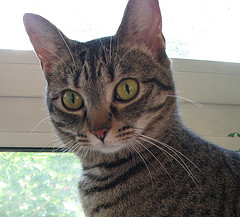
\includegraphics[width=1cm]{figures/cat1.png}};
    
    \coordinate (input2_c) at ($(input_bl) + (2*\inputPad + \imgSize * 1.5, \inputPad + \imgSize / 2)$);
    \node[inner sep=0pt] (input2) at (input2_c) {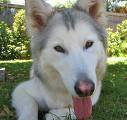
\includegraphics[width=1cm]{figures/dog.png}};
    
    \coordinate (input3_c) at ($(input_bl) + (\inputPad + \imgSize / 2, 2*\inputPad + \imgSize * 1.5)$);
    \node[inner sep=0pt] (input3) at (input3_c) {
\includegraphics[width=1cm]{figures/laptop.png}};
    
    \coordinate (input4_c) at ($(input_bl) + (2*\inputPad + \imgSize * 1.5, 2*\inputPad + \imgSize * 1.5)$);
    \node[inner sep=0pt] (input4) at (input4_c) {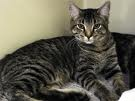
\includegraphics[width=1cm]{figures/cat2.png}};
    
    \coordinate (input_txt_c) at ($(input_bl) + (\inputPad * 1.5 + \imgSize, 3*\inputPad + 2*\imgSize + 0.1)$);
    \node[] (input_txt) at (input_txt_c) {Inputs};
    
    \coordinate (encoder_c) at ($(input_cr) + (2, 0)$);
    \node[draw, thick, inner sep=0.25cm, align=center, rounded corners, fill=blue!50] (encoder) at (encoder_c) {Encoder \\ Network};
    
    \coordinate (output_cl) at ($(encoder_c) + (2, 0)$);
    \coordinate (output_similar_bl) at ($(output_cl) + (0,0.125)$);
    \coordinate (output_similar_cl) at ($(output_similar_bl) + (0, \imgSize / 2 + \inputPad)$);
    \coordinate (output_similar_tr) at ($(output_similar_bl) + (2 * \imgSize + \inputPad * 3, \imgSize + 2 * \inputPad)$);
    \draw[thick, rounded corners, color=green] (output_similar_bl) rectangle (output_similar_tr);
    
    \coordinate (output_similar1_c) at ($(output_similar_bl) + (\inputPad + \imgSize / 2, \inputPad + \imgSize / 2)$);
    \node[inner sep=0pt] (output_similar1) at (output_similar1_c) {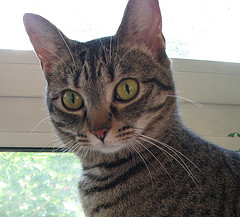
\includegraphics[width=1cm]{figures/cat1.png}};
    
    \coordinate (output_similar2_c) at ($(output_similar_bl) + (2*\inputPad + \imgSize * 1.5, \inputPad + \imgSize / 2)$);
    \node[inner sep=0pt] (output_similar2) at (output_similar2_c) {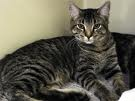
\includegraphics[width=1cm]{figures/cat2.png}};
    
    \coordinate (text_similar_c) at ($(output_similar_tr) + (0.25, -\imgSize / 2 - \inputPad)$);
    \node[anchor=west, color=green] at (text_similar_c) {Similar};
    
    \coordinate (output_unsimilar_bl) at ($(output_cl) - (0,0.125 + \imgSize + 2 * \inputPad)$);
    \coordinate (output_unsimilar_cl) at ($(output_unsimilar_bl) + (0, \imgSize / 2 + \inputPad)$);
    \coordinate (output_unsimilar_tr) at ($(output_unsimilar_bl) + (2 * \imgSize + \inputPad * 3, \imgSize + 2 * \inputPad)$);
    \draw[thick, rounded corners, color=red] (output_unsimilar_bl) rectangle (output_unsimilar_tr);
    
    \coordinate (output_unsimilar1_c) at ($(output_unsimilar_bl) + (\inputPad + \imgSize / 2, \inputPad + \imgSize / 2)$);
    \node[inner sep=0pt] (output_unsimilar1) at (output_unsimilar1_c) {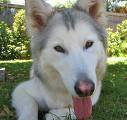
\includegraphics[width=1cm]{figures/dog.png}};
    
    \coordinate (output_unsimilar2_c) at ($(output_unsimilar_bl) + (2*\inputPad + \imgSize * 1.5, \inputPad + \imgSize / 2)$);
    \node[inner sep=0pt] (output_unsimilar2) at (output_unsimilar2_c) {
\includegraphics[width=1cm]{figures/laptop.png}};
    
    \coordinate (text_unsimilar_c) at ($(output_unsimilar_tr) + (0.25, -\imgSize / 2 - \inputPad)$);
    \node[anchor=west, color=red] at (text_unsimilar_c) {Not Similar};
    
    \draw[thick, ->] (input_cr) -- (encoder);
    \draw[thick, ->] (encoder.east) -- (output_similar_cl);
    \draw[thick, ->] (encoder.east) -- (output_unsimilar_cl);
    

\end{tikzpicture}
    \caption[Contrastive Learning]{The general contrastive learning task in the domain of image data. Different images are fed through an encoder network that predicts whether or not two images are similar or not. Images are from \textit{ImageNet} \cite{imagenet_cvpr09}.}
    \label{fig:contrastive_learning}
\end{figure}

As explained earlier labels can be created automatically using a self-supervised learning task. By combining self-supervised and contrastive learning it is possible to create a fully autonomous learning framework for similarities without the need for human annotation. This makes it possible to scale the training dataset to a much larger amount than in a fully supervised scenario. The way that we make use of this property is to create two augmented views from the same input and train the network to become invariant to those augmentations, meaning it will produce similar vectors for augmented views, but not for two completely unrelated views. This concept will be explained in more detail in Chapter \ref{chapter:claudio}.

\subsection{Transfer Learning}

Learning basic concepts first and applying those concepts to other tasks later on is an important part of deep learning research today. Transfer Learning can be seen as an extension to other learning paradigms that enables the transference of knowledge from one domain to another \cite{yang_zhang_dai_pan_2020}. A method for transfer learning of neural networks was proposed as early as 1993 by L. Y. Pratt \cite{NIPS1992_641} and is described in more detail in Algorithm \ref{alg:transfer}.

The basic idea behind transfer learning is that a neural network $f \circ g$, where $f$ is an arbitrary network architecture called encoder network that outputs vectors and $g$ is a small fully connected network called classification head that takes in the outputs of $f$ and produces predictions in the target domain. This network can be trained on a dataset $(X,y)$, containing training inputs $X$ and training outputs $y$, for example, images and the class of the depicted object in each image. During training the network $f$ learns general low-level features of image recognition while $g$ learns to map those features to the desired output $y$.

Now consider a second domain of image classification $(X',y')$ where $X'$ is of the same kind as $X$. Instead of training an entirely new network of the aforementioned structure, one can instead take the encoder network $f$ trained on the other dataset and transfer it into a new architecture $f \circ g'$ where $g'$ is a new classification head that takes in the outputs of $f$ and produces predictions in the new target domain $y'$. This is possible because the underlying data of both datasets share similar features, like edges and objects. The encoder network $f$ learns those features from the first dataset and transfers the knowledge to the second dataset. Shaha et al. \cite{shaha2018transfer} showed that using transfer learning on neural networks robust features can be transferred between multiple vision tasks. Figure \ref{fig:transfer_learning} shows this idea in a single diagram.

\begin{figure}[t]
    \centering
    \begin{tikzpicture}
    % global variables
    \definecolor{red}{RGB}{219, 50, 54}
    \definecolor{yellow}{RGB}{244, 194, 13}
    \definecolor{blue}{RGB}{72, 133, 237}
    \definecolor{green}{RGB}{60, 186, 84}
    \definecolor{orange}{RGB}{230, 122, 22}
    \definecolor{purple}{RGB}{145, 91, 145}
    \definecolor{grey}{RGB}{211, 211, 211}
    
    \tikzmath{
        \boxW = 11;
        \boxH = 2.5;
        \boxD = 0.25;
        \embeddingW = 3;
        \embeddingH = 1.5;
        \headW = 1.75;
        \pad = 2;
        \dArrow = 1;
    }
    
    % pretraining
    
    \coordinate (pretrain_bl) at (0,0);
    \coordinate (pretrain_c) at ($(pretrain_bl) + (\boxW / 2, \boxH / 2)$);
    \coordinate (pretrain_tr) at ($(pretrain_bl) + (\boxW, \boxH)$);
    \draw[rounded corners, thick] (pretrain_bl) rectangle (pretrain_tr);
    
    \coordinate (pretrain_text) at ($(pretrain_c) - (\boxW / 2 - 0.25, -0.75)$);
    \node[anchor=west, thick] at (pretrain_text) {1. Pre-training};
    
    \coordinate (data_p) at ($(pretrain_c) - (\boxW / 2 - \pad, 0)$);
    \node[align=left] (data_p_node) at (data_p) {$(X,y)$};
    
    \coordinate (embedding_p_cl) at ($(data_p) + (\dArrow,0)$);
    \coordinate (embedding_p_c) at ($(embedding_p_cl) + (\embeddingW / 2,0)$);
    \coordinate (embedding_p_cr) at ($(embedding_p_cl) + (\embeddingW,0)$);
    \coordinate (embedding_p_bl) at ($(embedding_p_cl) - (0,\embeddingH / 2)$);
    \coordinate (embedding_p_tr) at ($(embedding_p_bl) + (\embeddingW,\embeddingH)$);
    \coordinate (embedding_p_bc) at ($(embedding_p_c) - (0,\embeddingH / 2)$);
    \coordinate (embedding_p_tc) at ($(embedding_p_c) + (0,\embeddingH / 2)$);
    \draw[rounded corners, thick, fill=yellow!50] (embedding_p_bl) rectangle (embedding_p_tr);
    \node[align=center, thick] at (embedding_p_c) {Encoder $f$};
    
    \coordinate (head_p_cl) at ($(embedding_p_cr) + (0.5, 0)$);
    \coordinate (head_p_c) at ($(head_p_cl) + (\headW / 2, 0)$);
    \coordinate (head_p_cr) at ($(head_p_cl) + (\headW, 0)$);
    \coordinate (head_p_bl) at ($(head_p_cl) - (0, \embeddingH / 2)$);
    \coordinate (head_p_tr) at ($(head_p_bl) + (\headW, \embeddingH)$);
    
    \draw[rounded corners, thick, fill=red!50] (head_p_bl) rectangle (head_p_tr);
    \node[align=center, thick] at (head_p_c) {Head $g$};
    
    \coordinate (cost_p_c) at ($(head_p_cr) + (\dArrow-0.25, 0)$);
    \node[right, thick] (cost_p_node) at (cost_p_c) {$\mathcal{L}_{pre}$};
    
    \draw[->,thick] (data_p_node) -- (embedding_p_cl);
    \draw[->,thick] (embedding_p_cr) -- (head_p_cl);
    \draw[->,thick] (head_p_cr) -- (cost_p_node);
    
    
    % transfer
    
    \coordinate (transfer_bl) at ($(pretrain_bl) - (0, \boxH + \boxD)$);
    \coordinate (transfer_c) at ($(transfer_bl) + (\boxW / 2, \boxH / 2)$);
    \coordinate (transfer_tr) at ($(transfer_bl) + (\boxW, \boxH)$);
    \draw[rounded corners, thick] (transfer_bl) rectangle (transfer_tr);
    
    \coordinate (transfer_text) at ($(transfer_c) - (\boxW / 2 - 0.25, -0.75)$);
    \node[align=left, anchor=west, thick] at (transfer_text) {2. Transfer};
    
    \coordinate (data_t) at ($(transfer_c) - (\boxW / 2 - \pad, 0)$);
    \node[align=left] (data_t_node) at (data_t) {$(X',y')$};
    
    \coordinate (embedding_t_cl) at ($(data_t) + (\dArrow,0)$);
    \coordinate (embedding_t_c) at ($(embedding_t_cl) + (\embeddingW / 2,0)$);
    \coordinate (embedding_t_cr) at ($(embedding_t_cl) + (\embeddingW,0)$);
    \coordinate (embedding_t_bl) at ($(embedding_t_cl) - (0,\embeddingH / 2)$);
    \coordinate (embedding_t_tr) at ($(embedding_t_bl) + (\embeddingW,\embeddingH)$);
    \coordinate (embedding_t_bc) at ($(embedding_t_c) - (0,\embeddingH / 2)$);
    \coordinate (embedding_t_tc) at ($(embedding_t_c) + (0,\embeddingH / 2)$);
    \draw[rounded corners, thick, fill=yellow!50] (embedding_t_bl) rectangle (embedding_t_tr);
    \node[align=center, thick] at (embedding_t_c) {Encoder $f$ \\ (frozen)};
    
    \coordinate (head_t_cl) at ($(embedding_t_cr) + (0.5, 0)$);
    \coordinate (head_t_c) at ($(head_t_cl) + (\headW / 2, 0)$);
    \coordinate (head_t_cr) at ($(head_t_cl) + (\headW, 0)$);
    \coordinate (head_t_bl) at ($(head_t_cl) - (0, \embeddingH / 2)$);
    \coordinate (head_t_tr) at ($(head_t_bl) + (\headW, \embeddingH)$);
    \coordinate (head_t_bc) at ($(head_t_c) - (0, \embeddingH / 2)$);
    
    \draw[rounded corners, thick, fill=green!50] (head_t_bl) rectangle (head_t_tr);
    \node[align=center, thick] at (head_t_c) {Head $g'$};
    
    \coordinate (cost_t_c) at ($(head_t_cr) + (\dArrow-0.25, 0)$);
    \node[right, thick] (cost_t_node) at (cost_t_c) {$\mathcal{L}_{transfer}$};
    
    \draw[->,thick] (data_t_node) -- (embedding_t_cl);
    \draw[->,thick] (embedding_t_cr) -- (head_t_cl);
    \draw[->,thick] (head_t_cr) -- (cost_t_node);
    
    % finetune
    
    % \coordinate (finetune_bl) at ($(transfer_bl) - (0, \boxH + \boxD)$);
    % \coordinate (finetune_c) at ($(finetune_bl) + (\boxW / 2, \boxH / 2)$);
    % \coordinate (finetune_tr) at ($(finetune_bl) + (\boxW, \boxH)$);
    % \draw[rounded corners, thick] (finetune_bl) rectangle (finetune_tr);
    
    % \coordinate (finetune_text) at ($(finetune_c) - (\boxW / 2 - 0.25, -0.75)$);
    % \node[align=left, anchor=west, thick] at (finetune_text) {3. Fine-tuneing};
    
    % \coordinate (data_f) at ($(finetune_c) - (\boxW / 2 - \pad, 0)$);
    % \node[align=left] (data_f_node) at (data_f) {$(X',y'$};
    
    % \coordinate (embedding_f_cl) at ($(data_f) + (\dArrow,0)$);
    % \coordinate (embedding_f_c) at ($(embedding_f_cl) + (\embeddingW / 2,0)$);
    % \coordinate (embedding_f_cr) at ($(embedding_f_cl) + (\embeddingW,0)$);
    % \coordinate (embedding_f_bl) at ($(embedding_f_cl) - (0,\embeddingH / 2)$);
    % \coordinate (embedding_f_tr) at ($(embedding_f_bl) + (\embeddingW,\embeddingH)$);
    % \coordinate (embedding_f_bc) at ($(embedding_f_c) - (0,\embeddingH / 2)$);
    % \coordinate (embedding_f_tc) at ($(embedding_f_c) + (0,\embeddingH / 2)$);
    % \draw[rounded corners, thick, fill=yellow!50] (embedding_f_bl) rectangle (embedding_f_tr);
    % \node[align=center, thick] at (embedding_f_c) {Encoder};
    
    % \coordinate (head_f_cl) at ($(embedding_f_cr) + (0.5, 0)$);
    % \coordinate (head_f_c) at ($(head_f_cl) + (\headW / 2, 0)$);
    % \coordinate (head_f_cr) at ($(head_f_cl) + (\headW, 0)$);
    % \coordinate (head_f_bl) at ($(head_f_cl) - (0, \embeddingH / 2)$);
    % \coordinate (head_f_tr) at ($(head_f_bl) + (\headW, \embeddingH)$);
    % \coordinate (head_f_tc) at ($(head_f_c) + (0, \embeddingH / 2)$);
    
    % \draw[rounded corners, thick, fill=green!50] (head_f_bl) rectangle (head_f_tr);
    % \node[align=center, thick] at (head_f_c) {$Head_t$};
    
    % \coordinate (cost_f_c) at ($(head_f_cr) + (\dArrow, 0)$);
    % \node[align=center, thick] (cost_f_node) at (cost_f_c) {$Cost_t$};
    
    % \draw[->,thick] (data_f_node) -- (embedding_f_cl);
    % \draw[->,thick] (embedding_f_cr) -- (head_f_cl);
    % \draw[->,thick] (head_f_cr) -- (cost_f_node);
    
    % % 
    
    \draw[|->,thick] ($(embedding_p_bc) - (0, 0.15)$) -- ($(embedding_t_tc) + (0, 0.15)$);
    % \draw[|->,thick] ($(embedding_t_bc) - (0, 0.15)$) -- ($(embedding_f_tc) + (0, 0.15)$);
    % \draw[|->,thick] ($(head_t_bc) - (0, 0.15)$) -- ($(head_f_tc) + (0, 0.15)$);
    
    
\end{tikzpicture}
    \caption[Transfer Learning Overview]{The two stages of transfer learning. The encoder network is transferred after pre-training from the first domain to the second domain. Head is usually a small fully-connected network.}
    \label{fig:transfer_learning}
\end{figure}

\begin{algorithm}
    \caption{A supervised transfer-learning framework}
    \label{alg:transfer}
    
    \begin{algorithmic}[1]
        \State \textbf{Input:} encoder network $f$, classification heads $g$ and $g'$, trainable parameters  $\boldsymbol{\theta}_f$, $\boldsymbol{\theta}_g$, $\boldsymbol{\theta}_{g'}$, pre-training dataset $(X,Y)$, transfer dataset $(X', Y')$, loss functions $\mathcal{L}_{pre}$, $\mathcal{L}_{transfer}$, learning rate $\alpha$
        \State Randomly initialize $\theta_f$ and $\theta_g$ \Comment{Stage 1: Pre-training}
        \While{not done}
            \State sample minibatch $(\boldsymbol{x},\boldsymbol{y}) \sim (X,Y)$
            \State compute $\mathcal{L}_{pre}$ from $g(f(\boldsymbol{x}))$ and $\boldsymbol{y}$
            \State $\boldsymbol{\theta}_{f \circ g} \gets \boldsymbol{\theta}_{f \circ g} - \alpha \nabla_{\theta_{f \circ g}} \mathcal{L}_{pre}$ \Comment{$\theta_{f \circ g}$ is the concatenation of $\theta_f$ and $\theta_g$}
        \EndWhile
        \State Randomly initialize $\boldsymbol{\theta}_{g'}$ \Comment{Stage 2: Transfer}
        \State freeze $\boldsymbol{\theta}_f$
        \While{not done}
            \State sample minibatch $(\boldsymbol{x'},\boldsymbol{y'}) \sim (X',Y')$
            \State compute $\mathcal{L}_{transfer}$ from $g'(f(\boldsymbol{x'}))$ and $\boldsymbol{y'}$
            \State $\boldsymbol{\theta}_{f \circ g'} \gets \boldsymbol{\theta}_{f \circ g'} - \alpha \nabla_{\theta_{f \circ g'}} \mathcal{L}_{transfer}$
        \EndWhile
        \State \textbf{return} $f \circ g'$
    \end{algorithmic}
\end{algorithm}

The need for transfer learning arises when the domain to be transferred to has little or no training data or when making mistakes in unknown situations is expensive, as is the case in self-driving cars \cite{fellicious2018transfer}. In our case transfer learning will be used to take the latent representations learned from self-supervision and apply them to downstream supervised tasks with low amounts of available training data. This approach is very common and has shown good results in recent years (\cite{dosovitskiy2015discriminative, oord2019representation, bachman2019learning}). A thorough survey of modern transfer learning techniques can be found in Pan et al. (2010) \cite{pan2010transfer}.

\section{Self-Supervised Loss Functions}\label{sec:ss_loss}

Expressing the similarity of entities in the real world is effortless for humans. Be it sound events, images, words, all can easily be compared to other entities of that same domain. For machines this task is different. Since understanding similarity involves a lot of contextual knowledge that machines do not possess, the question if two entities are similar becomes much harder to answer for an algorithm. Self-supervised learning tries to bridge that knowledge gap by transforming complex real-world entities into a more simple representation that a machine can process. This representation is usually in the form of vectors. There are many ways of calculating the similarity of two vectors. Equations \ref{eq:euclidian_distance}, \ref{eq:manhattan_distance}, \ref{eq:cosine_similarity} describe three of the most common distance measures for vectors: \textit{euclidian distance}, \textit{manhattan distance} and \textit{cosine similarity}. Note that $s_{cosine}(p,q)$ is actually a similarity metric where $1$ is equal to the most similarity and $-1$ to the least similarity. One can simply convert it to a distance: $d_{cosine}(p,q) = 1 - s_{cosine}(p,q)$, but this is commonly not used. It is called cosine similarity because the result matches the cosine of the angle between the two vectors.

\begin{equation}
   d_{euclidian}(\mathbf{p},\mathbf{q}) = \lVert \mathbf{p,q} \rVert_2 = \sum_{i=1}^{n} \sqrt{(p_i - q_i)^2},\;\;\; \in \mathbb{R}^+
   \label{eq:euclidian_distance}
\end{equation}

\begin{equation}
   d_{manhattan}(\mathbf{p},\mathbf{q}) = \lVert \mathbf{p,q} \rVert_1 = \sum_{i=1}^{n} |p_i - q_i|,\;\;\;\;\;\;\; \in \mathbb{R}^+
   \label{eq:manhattan_distance}
\end{equation}

\begin{equation}
   s_{cosine}(\mathbf{p},\mathbf{q}) = \frac{\mathbf{p} \cdot \mathbf{q}}{\lVert \mathbf{p} \rVert \lVert \mathbf{q} \rVert} = \frac{\sum_{i=1}^{n}p_i q_i}{\sqrt{\sum_{i=1}^{n}p_i^2} \sqrt{\sum_{i=1}^{n}q_i^2}},\;\;\; \in [-1,1]
   \label{eq:cosine_similarity}
\end{equation}

In the following subsections we look at two loss functions that implement these distance metrics to give self-supervised algorithms a way to learn good vector representations. A loss function is a mathematical way of expressing a certain target for a neural network to train towards to. Stochastic gradient descent works by minimizing this loss function over time using stochastically sampled batches of data.

\subsection{Triplet Margin Loss}\label{subsec:tirplet}

As the name suggests the \textit{Triplet Margin Loss} requires triplets of input data points. These data points are called anchor $A$, positive $P$ and negative $N$. The positive is supposed to be of high similarity to the anchor, whereas the negative is supposed to be of no or low similarity to the anchor. Equation \ref{eq:triplet_loss} describes this notion in mathematical terms.

\begin{equation}
   \mathcal{L}(A,P,N) = max\Big( \lVert f(A), f(P) \rVert_2 - \lVert f(A), f(N) \rVert_2 + \alpha, 0 \Big)
   \label{eq:triplet_loss}
\end{equation}

This loss becomes larger the higher the distance between $A$ and $P$ and the lower the distance between $A$ and $N$. 
Here the euclidean distance is used but any distance function can be applied. By minimizing this loss the network is forced to learn representations that increase the distance to $N$ and decrease the distance to $P$, relative to $A$. Figure \ref{fig:triplet_training} shows how such representations could look like before and after learning. Note that usually a margin hyperparameter $\alpha$ is used to better distinguish positive from negatives, it’s effect can be seen in \ref{subfig:triplet_after}.

\begin{figure}[h!]
  \centering
  \begin{subfigure}[b]{0.49\linewidth}
    \centering
    \scalebox{0.75}{\begin{tikzpicture}
    \definecolor{red}{RGB}{219, 50, 54}
    \definecolor{yellow}{RGB}{244, 194, 13}
    \definecolor{blue}{RGB}{72, 133, 237}
    \definecolor{green}{RGB}{60, 186, 84}
    \definecolor{orange}{RGB}{230, 122, 22}
    \definecolor{purple}{RGB}{145, 91, 145}
    \definecolor{grey}{RGB}{211, 211, 211}
    
    \tikzstyle{blue}=[circle,fill,inner sep=4pt,color=blue!50]
    \tikzstyle{red}=[fill,inner sep=6pt,color=red!50]
    \tikzstyle{yellow}=[inner sep=3pt,color=yellow!50, regular polygon,regular polygon sides=3, fill]
    
    \tikzmath {
        \dbox = 0.75;
    }
    
    \begin{axis}[
        axis lines=middle,
        grid=major,
        xmin=0,
        xmax=4,
        ymin=0,
        ymax=4,
        tick style={very thick},
        xticklabels={,,},
        yticklabels={,,}
    ]
    \node[circle, thick, draw, inner sep=40pt, fill=grey] at (axis cs:2,2) {};
    \node[circle, thick, draw, inner sep=50pt] at (axis cs:2,2) {};
    \node[blue] at (axis cs:2,2) {};
    \node[blue] at (axis cs:1.7,1) {};
    \node[blue] at (axis cs:2.9,2.7) {};
    \node[blue] at (axis cs:2.7,1.3) {};
    \node[red] at (axis cs:1.5,1.9) {};
    \node[yellow] at (axis cs:1,3) {};
    \end{axis}

\end{tikzpicture}}
    \caption{Before training}
  \end{subfigure}
  \begin{subfigure}[b]{0.49\linewidth}
    \centering
    \scalebox{0.75}{\begin{tikzpicture}
    \definecolor{red}{RGB}{219, 50, 54}
    \definecolor{yellow}{RGB}{244, 194, 13}
    \definecolor{blue}{RGB}{72, 133, 237}
    \definecolor{green}{RGB}{60, 186, 84}
    \definecolor{orange}{RGB}{230, 122, 22}
    \definecolor{purple}{RGB}{145, 91, 145}
    \definecolor{grey}{RGB}{211, 211, 211}
    
    \tikzstyle{blue}=[circle,fill,inner sep=4pt,color=blue!50]
    \tikzstyle{red}=[fill,inner sep=6pt,color=red!50]
    \tikzstyle{yellow}=[inner sep=3pt,color=yellow!50, regular polygon,regular polygon sides=3, fill]
    
    \tikzmath {
        \dbox = 0.75;
    }
    
    \begin{axis}[
        axis lines=middle,
        grid=major,
        xmin=0,
        xmax=4,
        ymin=0,
        ymax=4,
        tick style={very thick},
        xticklabels={,,},
        yticklabels={,,}
    ]
    \node[circle, thick, draw, inner sep=25pt, fill=grey] at (axis cs:2,2) {};
    \node[circle, thick, draw, inner sep=35pt] at (axis cs:2,2) {};
    \node[blue] at (axis cs:2,2) {};
    \node[blue] at (axis cs:1.7,1.4) {};
    \node[blue] at (axis cs:2.3,2.1) {};
    \node[blue] at (axis cs:2.4,1.7) {};
    \node[red] at (axis cs:0.8,1.7) {};
    \node[yellow] at (axis cs:1.8,3.4) {};
    
    \node[] (margin) at (axis cs:3,3.5) {Margin};
    \draw[->, thick] (margin) -- (axis cs:2.3,3);
    
    \end{axis}

\end{tikzpicture}}
    \caption{After training}
    \label{subfig:triplet_after}
  \end{subfigure}
  \caption[Triplet loss example]{\textbf{Left}: Potential latent representations of input data points before training. They are mapped randomly into the latent space with no clear boundary. \textbf{Right}: After training with the triplet loss representations of the same class are pulled together while other classes are pushed apart. A margin zone, controlled by the margin hyperparameter, separates uncorrelated samples from correlated ones.}
  \label{fig:triplet_training}
\end{figure}

Since its first proposal in 2009 by Weinberger et al. \cite{Weinberger09distancemetric} the triplet loss is one of the most used loss functions for self-supervised learning. One major drawback of triplet loss is the fact that for randomly chosen inputs the loss approaches 0 very quickly since for most randomly chosen inputs $d(A,N) > d(A,P)$. These examples become irrelevant for training once this threshold is reached. Therefore a novel technique called online hard negative triplet mining was introduced by Schroff et al. \cite{Schroff_2015}. Online hard negative triplet mining ensures consistently increasing difficulty of triplets as the network trains but it requires one to track all comparisons and build up a memory bank that stores previous results. This is very inefficient and therefore more modern approaches try to replace it with simpler and more effective methods.

\subsection{Normalized Temperature-Scaled Cross Entropy}\label{subsec:ntxent}

\gls{ntxent} loss was first proposed by Sohn in 2016 \cite{sohn2016improved} but was coined \textit{NT-Xent} only recently by Chen et al. \cite{chen2020simple}. It was found that triplet loss functions "often suffer from slow convergence and poor local optima, partially due to that the loss function employs only one negative example while not interacting with the other negative classes per each update" \cite{sohn2016improved}. To deal with this issue, \gls{ntxent} loss takes one positive example and multiple negative examples per training step. The loss is defined as follows:

\begin{equation}
   \ell(i,j) = -\log \tfrac{\exp(s_{i,j}/\tau)}{\sum_{k=1}^{2N} \mathbb{1}_{[k \neq i]} \exp(s_{i,k} / \tau)}
   \label{eq:ntxent_loss}
\end{equation}

Here $\mathbb{1}$ is the indicator function which evaluates to 1 only if $k \neq i$ (the similarity of an input to itself is always 1 and therefore discarded). Usually for this loss $s_{i,j}$ denotes the cosine similarity of two vector representations but any similarity measure can be used. $\tau$ is a temperature hyperparameter used to expand the range of the exponential. This helps in stabilizing training. One can clearly see that this loss closely resembles a softmax distribution trying to maximize agreement of similar pairs.

The \gls{ntxent} loss has gained a lot of popularity since the release of \gls{simclr} (\cite{tu2020aag}, \cite{giorgi2020declutr}, \cite{apoorv2020speechembeddings}), mainly due to it scaling well to large batch sizes. This can be leveraged by ever-increasing memory sizes in deep learning specific processing units and better distribution strategies. Because of this and the fact that it does not require explicit example mining, we believe that \gls{ntxent} will replace triplet loss in most applications for self-supervised learning.

\section{Neural Networks for Audio Data}\label{sec:nn_audio}

Vibration is a repetitive motion relative to an equilibrium point \cite{nopdanai2017vibration}. Sound is therefore the vibration of molecules, usually air molecules, that is picked up by our ears and transformed into electrical signals that are then perceived by our brains. A similar thing happens when we try to digitize sound. First, a transducer converts sound into an electrical signal. This continuous signal is then transformed into a discrete signal by an \textit{Analog-to-digital converter} (ADC). The signal is periodically quantized to create a stream of samples. This way of digitally representing an analog signal is called \gls{pcm}.

Quantization maps a certain amplitude of an analog signal to a digital integer value, represented as a sequence of bits. The higher the number of bits per integer, also known as the bit-depth, the lower the error introduced by quantization. The frequency of this quantization is called the sampling frequency, usually denoted in kHz. The sampling frequency and the quantization error are the major factors of the quality of the digital audio signal. The higher the sampling rate and the bit-depth, the better the quality, but the more space is required to store the audio. In today's recordings, a sampling rate of 44.1kHz and a bit-depth of 16bit is most commonly used.

The resulting sequence of integer values can then be fed into a neural network for further processing. Unfortunately, classical network architectures are practically limited by the number of input values. A fully connected network with a single hidden layer consisting of 2048 hidden neurons would require more than 270 million weights to process a 3-second audio clip sampled at 44.1kHz. Nowadays it is common to make use of the time-series quality of audio data and use architectures that are specialized in this domain as shown in Lezhenin et al. \cite{lezhenin2019urban} or Zhao et al. \cite{zhao2019speechtransformer}.

Another common approach is to exploit the local dependency of samples in an audio signal by first applying convolutional layers to reduce the input dimensionality while preserving as much information as possible. It was also found that fully convolutional networks can produce remarkable results without any need for time-dependent computation \cite{fu2017raw}. Most of the architectures used today are combinations of the three. All of these network types can be used with one-dimensional data, as most recently shown in \cite{dhariwal2020jukebox} but are more often used with two-dimensional inputs. We therefore always transform our input signal using the Short-time Fourier transform described in \ref{sec:fft} to create a two-dimensional matrix where $x_{i,j}$ represents the $i$th Fourier coefficient at timestep $j$. This process reduces the number of timesteps significantly and thus reduces the size of the networks. The final goal is to produce a single vector that best describes the data it is trying to represent. In the remaining subsections, we dive deeper into the theory of all three architectures.

\subsection{Convolutional Neural Network}

The kernel convolution for two-dimensional inputs used in a \gls{cnn} is defined in Equation \ref{eq:kernel_convolution} for discrete inputs.

\begin{equation}
   g(x,y) = \omega * f(x,y) = \sum_{dx=-a}^a \sum_{dy=-b}^b \omega (dx,dy) f(x + dx, y + dy)
   \label{eq:kernel_convolution}
\end{equation}

Here $\omega$ is the kernel matrix ranging from $[-a,-b]$ to $[a,b]$. $f(x,y)$ is a pixel of an input image $f$. The kernel $\omega$ is shifted over the two dimensions $x$ and $y$ of $f$ and repeatedly multiplied with a part of the input image centered around $f(x,y)$. In the end, the resulting output pixels $g(x,y)$ are put back together to produce a filtered output $g$. Note that the kernel does not have to move one pixel at a time but can move any desired distance per step. This distance is called stride. If the stride is larger than 1, the size of the output image is reduced.

The kernel matrix is composed of learnable weights. Training such a network using backpropagation was first proposed by LeCun et al. in 1989 \cite{lecun1989backpropagation} and has since seen magnificent results in image-related tasks but also in other domains like audio.

The advantage of this compared to fully connected layers is that the size of the kernel matrix is not determined by the size of the input, so larger input matrices do not necessarily require more trainable weights. This kernel convolution is usually followed by a non-linear activation function. The most prominent activation function for \glspl{cnn} is the \gls{relu}, proposed by Hinton et al. \cite{icml2010relu} and denoted in Equation \ref{eq:relu}.

\begin{equation}
   f(x)= 
    \begin{cases}
        x,& \text{if } x\ge 0\\
        0,              & \text{otherwise}
    \end{cases}
   \label{eq:relu}
\end{equation}

Due to its non-saturating gradient, it accelerates stochastic gradient-based learning, as opposed to alternatives like sigmoid or tanh \cite{NIPS2012_4824}. Note that this comes with a drawback that neurons can potentially die out, meaning they can enter states that produce negative outputs for all inputs and therefore never produce any gradient other than 0. There exist many alternatives that mitigate this issue, like the \textit{leaky ReLU} that assigns small values for inputs lower than zero, so therefore always producing some gradient. In practice, however, this problem is often ignored since large networks can cope with a few dead neurons.

To further reduce dimensionality to subsequent layers, \glspl{cnn} commonly employ pooling after each convolution step. As evaluated in Scherer et al. \cite{scherer2010maxpool}, max-pooling, which returns the maximum value of a given receptive field, is vastly superior to other pooling techniques. Figure \ref{fig:cnn} shows a single stack of convolution, \gls{relu} and max-pooling layers. In practice, there are many such stacks combined to produce a condensed set of features that best describes the given input and that can be used for further downstream tasks such as classification.

\glspl{cnn} for time series classification were first introduced by Wang et al. in 2017 \cite{wang2016time}. They form a strong baseline, that is difficult to beat on arbitrary data without heavy fine-tuning to a specific task. Even though \glspl{cnn} are extremely powerful in finding local dependencies in data, they fail to learn dependencies that are far apart. This is due to the kernel convolution only looking at specific areas of the input one at a time.

\begin{figure}[!h]
    \centering
    \begin{tikzpicture}
    \definecolor{red}{RGB}{219, 50, 54}
    \definecolor{yellow}{RGB}{244, 194, 13}
    \definecolor{blue}{RGB}{72, 133, 237}
    \definecolor{green}{RGB}{60, 186, 84}
    \definecolor{orange}{RGB}{230, 122, 22}
    \definecolor{purple}{RGB}{145, 91, 145}
    \definecolor{grey}{RGB}{211, 211, 211}
    
    \tikzmath {
        \boxW = 2;
        \boxH = 2;
        \dH = 0.1;
        \dW = 0.1;
        \convW = 2;
        \convH = 2;
        \dLayer = 3.75;
        \shrink = 0.8;
        \reluW = 0.5;
        \recD = 0.5;
        \recPad = 0.25;
    }
    
    \coordinate (input_bl) at (0,0);
    \coordinate (input_tr) at ($(input_bl) + (\boxW, \boxH)$);
    
    \coordinate (input_rec_bl) at ($(input_bl) + (\boxW - \recD - \recPad, \recPad)$);
    \coordinate (input_rec_tr) at ($(input_rec_bl) + (\recD, \recD)$);
    
    \draw[thick] (input_rec_bl) rectangle (input_rec_tr);
    
    \draw[thick] (input_bl) rectangle (input_tr);
    
    \foreach \i in {5,...,1}
    {
        \coordinate (kernel_bl) at ($(input_bl) + (\dLayer - \dW * \i, \dH * \i)$);
        \coordinate (kernel_tr) at ($(kernel_bl) + (\convW * \shrink, \convH * \shrink)$);
        \draw[thick, fill=white] (kernel_bl) rectangle (kernel_tr);
    }
    
    
    \coordinate (conv_bl) at ($(input_bl) + (\dLayer, 0)$);
    \coordinate (conv_tr) at ($(conv_bl) + (\convW * \shrink, \convH * \shrink)$);
    \coordinate (conv_cr) at ($(conv_bl) + (\convW * \shrink, \boxH / 2)$);
    \draw[thick, fill=white] (conv_bl) rectangle (conv_tr);
    
    \coordinate (input_rec_dest) at ($(conv_bl) + (\convW * \shrink - 0.25, 0.25)$);
    \coordinate (conv_rec_bl) at ($(conv_tr) - (0.5, 0.5)$);
    \coordinate (conv_rec_tr) at ($(conv_rec_bl) + (0.35, 0.35)$);
    \draw[thick] (conv_rec_bl) rectangle (conv_rec_tr);
    
    
    
    \coordinate (relu_bl)  at ($(conv_bl) + (2.5, 0)$);
    \coordinate (relu_c)  at ($(relu_bl) + (\reluW / 2, \boxH / 2)$);
    \coordinate (relu_tr) at ($(relu_bl) + (\reluW, \boxH)$);
    \coordinate (relu_lc) at ($(relu_bl) + (0, \boxH / 2)$);
    \node[rotate=90] at (relu_c) {ReLU};
    
    \draw[thick] (relu_bl) rectangle (relu_tr);
    %\draw[|->, thick] ($(conv_cr) + (0.15, 0)$) -- ($(relu_lc) - (0.15, 0)$);
    
    \foreach \i in {5,...,1}
    {
        \coordinate (pool_bl) at ($(relu_bl) + (2 - \dW * \i, \dH * \i)$);
        \coordinate (pool_tr) at ($(pool_bl) + (\convW * \shrink * \shrink, \convH * \shrink * \shrink)$);
        \draw[thick, fill=white] (pool_bl) rectangle (pool_tr);
    }
    
    \coordinate (pool_bl) at ($(relu_bl) + (2, 0)$);
    \coordinate (pool_tr) at ($(pool_bl) + (\convW * \shrink * \shrink, \convH * \shrink * \shrink)$);
    \coordinate (pool_cr) at ($(pool_bl) + (\convW * \shrink * \shrink, \boxH / 2)$);
    \draw[thick, fill=white] (pool_bl) rectangle (pool_tr);
    
    
    \coordinate (conv_rec_dest) at ($(pool_tr) - (0.25, 0.25)$);
    
    \draw[thick, dashed] (input_rec_bl) -- (input_rec_dest);
    \draw[thick, dashed] (input_rec_tr) -- (input_rec_dest);
    
    \draw[thick, dashed] (conv_rec_bl) -- (conv_rec_dest);
    \draw[thick, dashed] (conv_rec_tr) -- (conv_rec_dest);
    
    \node[] at ($(conv_bl) - (0.8, 0.3)$)  {Convolution};
    \node[] at ($(pool_bl) - (0.8, 0.3)$) {Pooling};
    
\end{tikzpicture}
    \caption[Convolution, ReLU and max-pool overview]{A single stack of a convolutional, ReLU and max-pooling layer. First $n$ filters are convoluted with the input, resulting in $n$ output channels. All output channels are then fed through a ReLU and finally max-pooled to further decrease the output size.}
    \label{fig:cnn}
\end{figure}

\subsection{Long Short-Term Memory}\label{subsec:lstm}

\gls{lstm} is a type of \gls{rnn} used for processing time-series data. It was first proposed by Hochreiter and Schmidhuber in 1997 \cite{hochreiter1997lstm}. A common problem for pre-LSTM \glspl{rnn} was to learn long-term temporal dependencies due to exponentially decaying gradients over time. To mitigate this issue \gls{lstm} employs a series of gates, described in Equation \ref{eq:lstm_forget} to \ref{eq:lstm_hidden}, that regulate the memory state of a cell.

\begin{equation}
   \mathbf{f}_t = \sigma (\mathbf{W}_f \mathbf{x}_t + \mathbf{U}_f \mathbf{c}_{t-1} + \mathbf{b}_f)
   \label{eq:lstm_forget}
\end{equation}

\begin{equation}
   \mathbf{i}_t = \sigma (\mathbf{W}_i \mathbf{x}_t + \mathbf{U}_i \mathbf{c}_{t-1} + \mathbf{b}_i)
   \label{eq:lstm_input}
\end{equation}

\begin{equation}
   \mathbf{o}_t = \sigma (\mathbf{W}_o \mathbf{x}_t + \mathbf{U}_o \mathbf{c}_{t-1} + \mathbf{b}_o)
   \label{eq:lstm_output}
\end{equation}

\begin{equation}
   \mathbf{c}_t = \mathbf{f}_t \circ \mathbf{c}_{t-1} + \mathbf{i}_t \circ tanh (\mathbf{W}_c \mathbf{x}_t + \mathbf{b}_c)
   \label{eq:lstm_context}
\end{equation}

\begin{equation}
   \mathbf{h}_t = \mathbf{o}_t \circ tanh (\mathbf{c}_t)
   \label{eq:lstm_hidden}
\end{equation}

Here $\sigma$ denotes the sigmoid function and $\circ$ denotes the element-wise vector multiplication. $\mathbf{x}_t \in \mathbb{R}^d$ is the input at time-step $t$, $ \mathbf{h}_t \in \mathbb{R}^h$ is the outputted hidden state at timestep $t$. $\mathbf{W}$, $\mathbf{U} \in \mathbb{R}^{h \times d}$ are traininable weights and $\mathbf{b} \in \mathbb{R}^h$ are trainable biases. $\mathbf{f}_t, \mathbf{i}_t, \mathbf{o}_t \in \mathbb{R}^h$ are intermediate vectors called gates. Figure \ref{fig:lstm_cell} shows how the different gates interact. At its core the cell state is described by Equation \ref{eq:lstm_context}: a new state $ \mathbf{c}_t$ is the sum of two terms. The first term $\mathbf{f}_t \circ  \mathbf{c}_{t-1}$ includes the forget gate $ \mathbf{f}_t$, which regulates when old state should be forgotten, while the second term $ \mathbf{i}_t \circ tanh ( \mathbf{W}_c  \mathbf{x}_t +  \mathbf{b}_c)$ includes the input gate $ \mathbf{i}_t$, which regulates when new information should be remembered.

\begin{figure}[!h]
    \centering
    \begin{tikzpicture}
    \definecolor{red}{RGB}{219, 50, 54}
    \definecolor{yellow}{RGB}{244, 194, 13}
    \definecolor{blue}{RGB}{72, 133, 237}
    \definecolor{green}{RGB}{60, 186, 84}
    \definecolor{orange}{RGB}{230, 122, 22}
    \definecolor{purple}{RGB}{145, 91, 145}
    \definecolor{grey}{RGB}{211, 211, 211}
    
    \tikzmath {
        \cellW = 9;
        \cellH = 4.5;
        \dSigmaW = 1.5;
        \dSigmaH = 0.5;
        \pad = 0.6;
    }
    
    \tikzstyle{a}=[thick,draw, minimum width=1cm, minimum height=0.5cm, fill=yellow!50]
    \tikzstyle{b}=[shape=circle,thick,draw,minimum size=0.5cm, fill=red!50]
    \tikzstyle{c}=[shape=rectangle,rounded corners,thick,draw,minimum height=0.5cm, fill=red!50]
    
    \coordinate (cell_bl) at (0,0);
    \coordinate (cell_tr) at ($(cell_bl) + (\cellW, \cellH)$);
    \draw[thick, rounded corners, fill=green!50] (cell_bl) rectangle (cell_tr);
    
    \coordinate (sigma_ft_c) at ($(cell_bl) + (\pad + 0.2, \pad + \dSigmaH)$);
    \node[a] (sigma_ft) at (sigma_ft_c) {\Large $\sigma$};
    
    \coordinate (sigma_it_c) at ($(sigma_ft) + (\dSigmaW, 0)$);
    \node[a] (sigma_it) at (sigma_it_c) {\Large $\sigma$};
    
    \coordinate (tanh_ct_c) at ($(sigma_it) + (\dSigmaW, 0)$);
    \node[a] (tanh_ct) at (tanh_ct_c) {$tanh$};
    
    \coordinate (sigma_ot_c) at ($(tanh_ct_c) + (\dSigmaW, 0)$);
    \node[a] (sigma_ot) at (sigma_ot_c) {\Large $\sigma$};
    
    \coordinate (ct_mul_c) at ($(sigma_ft_c) + (0, \cellH - 2 * \pad - \dSigmaH)$);
    \node[b] (ct_mul) at (ct_mul_c) {$\times$};
    
    \path let \p1=(tanh_ct_c),\p2=(ct_mul_c) in coordinate (ct_plus_c) at (\x1,\y2);
    \node[b] (ct_plus) at (ct_plus_c) {$+$};
    
    \coordinate (ct_mul_it_c) at ($(tanh_ct_c) + (0, 1.2)$);
    \node[b] (ct_mul_it) at (ct_mul_it_c) {$\times$};
    
    \coordinate (ot_mul_c) at ($(sigma_ot_c) + (\dSigmaW, 1.2)$);
    \node[b] (ot_mul) at (ot_mul_c) {$\times$};
    
    \coordinate (ot_tanh_c) at ($(ot_mul_c) + (0, 0.8)$);
    \node[c] (ot_tanh) at (ot_tanh_c) {$tanh$};
    
    \path let \p1=(cell_bl),\p2=(ct_mul_c) in coordinate (c_input_border) at (\x1,\y2);
    \coordinate (c_input_c) at ($(c_input_border) - (1,0)$);
    \node[] (c_input) at (c_input_c) {$c_{t-1}$};
    
    \coordinate (h_input_c) at ($(cell_bl) + (-1, \pad)$);
    \node[] (h_input) at (h_input_c) {$h_{t-1}$};
    
    \coordinate (x_input_c) at ($(cell_bl) + (0.5, -0.75)$);
    \node[] (x_input) at (x_input_c) {$x_t$};
    
    \coordinate (h_output1_c) at ($(h_input_c) + (1 + \cellW + 1, 0)$);
    \node[] (h_output1) at (h_output1_c) {$h_t$};
    
    \coordinate (c_output_c) at ($(c_input_c) + (1 + \cellW + 1, 0)$);
    \node[] (c_output) at (c_output_c) {$c_t$};
    
    \coordinate (h_output2_c) at ($(cell_tr) + (-0.75, 0.75)$);
    \node[] (h_output2) at (h_output2_c) {$h_t$};
    
    \draw[thick] (c_input) -- (ct_mul);
    \draw[thick] (ct_mul) -- (ct_plus);
    \draw[thick, ->] (sigma_ft) -- (ct_mul);
    \draw[thick, ->] (ct_plus) -- (c_output);
    \draw[thick] (tanh_ct) -- (ct_mul_it);
    \draw[thick, ->] (ct_mul_it) -- (ct_plus);
    
    \path let \p1=(sigma_ot_c),\p2=(h_input_c) in coordinate (h_input_path1) at (\x1,\y2);
    
    \draw[thick, rounded corners] (h_input) -- (h_input_path1) -- (sigma_ot);
    
    \path let \p1=(sigma_ft_c),\p2=(h_input_c) in coordinate (h_input_sigma_ft) at (\x1,\y2);
    \path let \p1=(sigma_it_c),\p2=(h_input_c) in coordinate (h_input_sigma_it) at (\x1,\y2);
    \path let \p1=(tanh_ct_c),\p2=(h_input_c) in coordinate (h_input_tanh_ct) at (\x1,\y2);
    
    \draw[thick] (h_input_sigma_ft) -- (sigma_ft);
    \draw[thick] (h_input_sigma_it) -- (sigma_it);
    \draw[thick] (h_input_tanh_ct) -- (tanh_ct);
    
    \path let \p1=(sigma_it_c),\p2=(ct_mul_it_c) in coordinate (it_path1) at (\x1,\y2);
    
    \draw[thick, rounded corners, ->] (sigma_it) -- (it_path1) -- (ct_mul_it);
    
    \path let \p1=(sigma_ot_c),\p2=(ot_mul_c) in coordinate (ot_path1) at (\x1,\y2);
    
    \draw[thick, rounded corners, ->] (sigma_ot) -- (ot_path1) -- (ot_mul);
    
    \path let \p1=(ot_mul_c),\p2=(h_output1_c) in coordinate (ot_output_path) at (\x1,\y2);
    
    \draw[thick, rounded corners, ->] (ot_mul) -- (ot_output_path) -- (h_output1);
    
    \path let \p1=(ot_tanh_c),\p2=(c_input_c) in coordinate (c_ot_path) at (\x1,\y2);
    \draw[thick] (c_ot_path) -- (ot_tanh);
    \draw[thick] (ot_tanh) -- (ot_mul);
    
    \path let \p1=(x_input_c),\p2=(h_input_c) in coordinate (x_input_path) at (\x1,\y2);
    
    \draw[thick] (x_input) -- (x_input_path);
    
    \path let \p1=(h_output2_c),\p2=(h_output1_c) in coordinate (h_output2_path1) at (\x1,\y2);
    
    \path let \p1=(h_output2_c),\p2=(c_input_c) in coordinate (h_output2_path2) at (\x1,\y2);
    
    \coordinate (h_output2_path3) at ($(h_output2_path2) - (0, 0.15)$);
    \coordinate (h_output2_path4) at ($(h_output2_path2) + (0, 0.15)$);
    
    \draw[thick] (h_output2_path1) -- (h_output2_path3);
    \draw[thick, ->] (h_output2_path4) -- (h_output2);
    
    \coordinate (ft_text) at ($(sigma_ft_c) + (-0.2,1.1)$);
    \node[] at (ft_text) {$f_t$};
    
    \coordinate (it_text) at ($(it_path1) - (0.2,0.2)$);
    \node[] at (it_text) {$i_t$};
    
    \coordinate (ot_text) at ($(ot_path1) - (0.2,0.2)$);
    \node[] at (ot_text) {$o_t$};
    
    % \coordinate (ct_text) at ($(ct_mul_it_c) - (0.2,0.6)$);
    % \node[] at (ct_text) {$c_t$};
\end{tikzpicture}
    \caption[LSTM cell Overview]{The flow through a LSTM cell. The last hidden state $h_t$ is used as the latent representation of the input.}
    \label{fig:lstm_cell}
\end{figure}

In Hinton et al. \cite{graves2013speech} the authors showed that \glspl{lstm} can be successfully used on audio data. But even though its performance on long time temporal dependencies is really strong, its computational speed is not as efficient as the other methods described in this section. This comes from the fact that a \gls{lstm} cell state $ \mathbf{c}_t$ depends on the previous cell state $ \mathbf{c}_{t-1}$. This makes the parallelization of \glspl{rnn} impossible and so the benefits of modern deep learning hardware cannot be leveraged.

\subsection{Self-Attention}

Self-Attention networks have gained a lot of popularity in the last two years mostly resulting from the success of Transformers in \gls{nlp}. This architecture was first proposed in the paper called "Attention is all you need" \cite{NIPS2017_7181}. The \textit{Transformer} is an encoder-decoder based architecture for sequence data that is not reliant on any recurrence whatsoever. This makes the model extremely parallelizable which in turn resulted in huge models being trained on big GPU-clusters in parallel \cite{brown2020language}. The results of these models raised the bar for state of the art models in almost all \gls{nlp} tasks by a significant amount. Figure \ref{fig:attention_mha} shows the Scaled Dot-Product Attention (often just called self-attention) and the \gls{mha}, both proposed by Vaswani et al. in the original \textit{Transformer} paper \cite{NIPS2017_7181}.

\begin{figure}[h!]
  \centering
  \begin{subfigure}[b]{0.49\linewidth}
    \centering
    \scalebox{1.0}{\begin{tikzpicture}
    \definecolor{red}{RGB}{219, 50, 54}
    \definecolor{yellow}{RGB}{244, 194, 13}
    \definecolor{blue}{RGB}{72, 133, 237}
    \definecolor{green}{RGB}{60, 186, 84}
    \definecolor{orange}{RGB}{230, 122, 22}
    \definecolor{purple}{RGB}{145, 91, 145}
    \definecolor{grey}{RGB}{211, 211, 211}
    
    \tikzstyle{a}=[thick, draw, minimum height=1, rounded corners]
    
    \tikzmath {
        \dbox = 0.75;
    }
    
    \coordinate (matmul1_c) at (0,0);
    \node[a, fill=purple!50] (matmul1) at (matmul1_c) {$\;$ MatMul $\;$};
    
    \coordinate (scale_c) at ($(matmul1_c) + (0, \dbox)$);
    \node[a, fill=yellow!50] (scale) at (scale_c) {$\;$ Scale $\;$};
    
    \coordinate (mask_c) at ($(scale_c) + (0, \dbox)$);
    \node[a, fill=blue!50] (mask) at (mask_c) {$\;$ Mask $\;$};
    
    \coordinate (softmax_c) at ($(mask_c) + (0, \dbox)$);
    \node[a, fill=green!50] (softmax) at (softmax_c) {$\;$ Softmax $\;$};
    
    \coordinate (matmul2_c) at ($(softmax_c) + (0.75, \dbox)$);
    \node[a, fill=purple!50] (matmul2) at (matmul2_c) {$\;\;\;$ MatMul $\;\;\;$};
    
    \coordinate (q_txt_c) at ($(matmul1_c) - (0.5, 1)$);
    \node[] (q_txt) at (q_txt_c) {$Q$};
    
    \coordinate (k_txt_c) at ($(q_txt_c) + (1, 0)$);
    \node[] (k_txt) at (k_txt_c) {$K$};
    
    \coordinate (v_txt_c) at ($(k_txt_c) + (1, 0)$);
    \node[] (v_txt) at (v_txt_c) {$V$};
    
    \draw[thick, ->] (q_txt) -- (q_txt|-matmul1.south);
    \draw[thick, ->] (k_txt) -- (k_txt|-matmul1.south);
    \draw[thick, ->] (v_txt) -- (v_txt|-matmul2.south);
    
    \draw[thick, ->] (matmul1) -- (scale);
    \draw[thick, ->] (scale) -- (mask);
    \draw[thick, ->] (mask) -- (softmax);
    \draw[thick, ->] (softmax) -- (softmax|-matmul2.south);
    
    \coordinate (empty_arr) at ($(matmul2_c) + (0, 0.5)$);
    \draw[thick, ->] (matmul2) -- (empty_arr);
    
    
    
\end{tikzpicture}}
    \caption{Scaled Dot-Product Attention}
  \end{subfigure}
  \begin{subfigure}[b]{0.49\linewidth}
    \centering
    \scalebox{1.0}{\begin{tikzpicture}
    \definecolor{red}{RGB}{219, 50, 54}
    \definecolor{yellow}{RGB}{244, 194, 13}
    \definecolor{blue}{RGB}{72, 133, 237}
    \definecolor{green}{RGB}{60, 186, 84}
    \definecolor{orange}{RGB}{230, 122, 22}
    \definecolor{purple}{RGB}{145, 91, 145}
    \definecolor{grey}{RGB}{211, 211, 211}
    
    \tikzstyle{a}=[thick, rounded corners]
    \tikzstyle{attention}=[thick, rounded corners, minimum width=4.5cm]
    
    \tikzmath {
        \dbox = 0.75;
        \dTxtLinear = 0.9;
        \dTxt = 1.7;
        \dLinears = 0.1;
        \dLayers = 1.2;
    }

    % QKV
    
    \coordinate (q_txt_c) at (0,0);
    \node[] (q_txt) at (q_txt_c) {$Q$};
    
    \coordinate (k_txt_c) at ($(q_txt_c) + (\dTxt, 0)$);
    \node[] (k_txt) at (k_txt_c) {$K$};
    
    \coordinate (v_txt_c) at ($(k_txt_c) + (\dTxt, 0)$);
    \node[] (v_txt) at (v_txt_c) {$V$};
    
    % Linear
    
    \coordinate (linear11_c) at ($(q_txt_c) + (0, \dTxtLinear)$);
    \node[a, draw=black!100, fill=grey!100] (linear11) at (linear11_c) {Linear};
    
    \coordinate (linear21_c) at ($(k_txt_c) + (0, \dTxtLinear)$);
    \node[a, draw=black!100, fill=grey!100] (linear21) at (linear21_c) {Linear};
    
    \coordinate (linear31_c) at ($(v_txt_c) + (0, \dTxtLinear)$);
    \node[a, draw=black!100, fill=grey!100] (linear31) at (linear31_c) {Linear};
    
    \begin{pgfonlayer}{background}
        \coordinate (linear12_c) at ($(linear11_c) + (\dLinears, \dLinears)$);
        \node[a, draw=black!70, fill=grey!70] (linear12) at (linear12_c){Linear};
        
        \coordinate (linear22_c) at ($(linear21_c) + (\dLinears, \dLinears)$);
        \node[a, draw=black!70, fill=grey!70] (linear22) at (linear22_c){Linear};
        
        \coordinate (linear32_c) at ($(linear31_c) + (\dLinears, \dLinears)$);
        \node[a, draw=black!70, fill=grey!70] (linear32) at (linear32_c){Linear};
    \end{pgfonlayer}
    
    \begin{pgfonlayer}{background2}
        \coordinate (linear13_c) at ($(linear12_c) + (\dLinears, \dLinears)$);
        \node[a, draw=black!40, fill=grey!40] (linear13) at (linear13_c){Linear};
        
        \coordinate (linear23_c) at ($(linear22_c) + (\dLinears, \dLinears)$);
        \node[a, draw=black!40, fill=grey!40] (linear23) at (linear23_c){Linear};
        
        \coordinate (linear33_c) at ($(linear32_c) + (\dLinears, \dLinears)$);
        \node[a, draw=black!40, fill=grey!40] (linear33) at (linear33_c){Linear};
    \end{pgfonlayer}
    
    % Attention
    \coordinate (attention1_c) at ($(linear21_c) + (0, \dLayers)$);
    \node[attention, align=center, draw=black!100, fill=purple!50] (attention1) at (attention1_c){Scaled Dot-Product \\ Attention};
    
    \begin{pgfonlayer}{background}
        \coordinate (attention2_c) at ($(attention1_c) + (\dLinears, \dLinears)$);
        \node[attention, align=center, draw=black!70, fill=purple!30] (attention2) at (attention2_c){Scaled Dot-Product \\ Attention};
    \end{pgfonlayer}
    
    \begin{pgfonlayer}{background2}
        \coordinate (attention3_c) at ($(attention2_c) + (\dLinears, \dLinears)$);
        \node[attention, align=center, draw=black!40, fill=purple!10] (attention3) at (attention3_c){Scaled Dot-Product \\ Attention};
    \end{pgfonlayer}
    
    % Concat
    
    \coordinate (concat_c) at ($(attention1_c) + (0, \dLayers)$);
    \node[a, align=center, draw=black!100, fill=yellow!50] (concat) at (concat_c){Concat};
    
    % Linear2
    
    \coordinate (linear_c) at ($(concat_c) + (0, 0.75)$);
    \node[a, align=center, draw=black!100, fill=grey!100] (linear) at (linear_c){Linear};
    
    \coordinate (final_c) at ($(linear_c) + (0, 0.5)$);
    
    % connections
    
    \draw[thick, ->] (q_txt) -- (q_txt|-linear11.south);
    \draw[thick, ->] (k_txt) -- (k_txt|-linear21.south);
    \draw[thick, ->] (v_txt) -- (v_txt|-linear31.south);
    
    \draw[thick, ->] (linear11) -- (linear11|-attention1.south);
    \draw[thick, ->] (linear21) -- (linear21|-attention1.south);
    \draw[thick, ->] (linear31) -- (linear31|-attention1.south);
    
    \begin{pgfonlayer}{background}
        \draw[thick, color=black!70, ->] (linear12) -- (linear12|-attention2.south);
        \draw[thick, color=black!70, ->] (linear22) -- (linear22|-attention2.south);
        \draw[thick, color=black!70, ->] (linear32) -- (linear32|-attention2.south);
    \end{pgfonlayer}
    
    \begin{pgfonlayer}{background2}
        \draw[thick, color=black!40, ->] (linear13) -- (linear13|-attention3.south);
        \draw[thick, color=black!40, ->] (linear23) -- (linear23|-attention3.south);
        \draw[thick, color=black!40, ->] (linear33) -- (linear33|-attention3.south);
    \end{pgfonlayer}
    
    \draw[thick, ->] (attention1) -- (attention1|-concat.south);
    \draw[thick, color=black!70, ->] (attention2) -- (attention2|-concat.south);
    \draw[thick, color=black!40, ->] (attention3) -- (attention3|-concat.south);
    
    \draw[thick, ->] (concat) -- (linear);
    \draw[thick, ->] (linear) -- (final_c);
\end{tikzpicture}}
    \caption{Multi-Head-Attention}
  \end{subfigure}
  \caption[Scaled Dot-Product Attention and Multi-Head-Attention]{The basic components of a self-attention block. In practice multiple Attention-blocks are stacked onto each other to produce better representations. Figures are from the original Transformer paper \cite{NIPS2017_7181}.}
  \label{fig:attention_mha}
\end{figure}

Self-attention is a mechanism in which each input of a sequence can compute a certain relationship to each other input. The input of the scaled dot product attention is a linear transformation of the inputs with three different, learnable matrices, called query, key and value. All three matrices have the same output dimension. \gls{mha} extends this concept by applying multiple such self-attention computations in parallel and concatenating the results. \gls{mha} is usually preceded and followed by linear transformations. Just like multiple kernel matrices in the same convolutional layer, \gls{mha} allows the network to learn multiple representations of the input at the same time, thus decreasing the probability that information is lost.

\section{Fast Fourier Transformation}\label{sec:fft}

\begin{figure}[t]
    \centering
    %% Creator: Matplotlib, PGF backend
%%
%% To include the figure in your LaTeX document, write
%%   \input{<filename>.pgf}
%%
%% Make sure the required packages are loaded in your preamble
%%   \usepackage{pgf}
%%
%% and, on pdftex
%%   \usepackage[utf8]{inputenc}\DeclareUnicodeCharacter{2212}{-}
%%
%% or, on luatex and xetex
%%   \usepackage{unicode-math}
%%
%% Figures using additional raster images can only be included by \input if
%% they are in the same directory as the main LaTeX file. For loading figures
%% from other directories you can use the `import` package
%%   \usepackage{import}
%%
%% and then include the figures with
%%   \import{<path to file>}{<filename>.pgf}
%%
%% Matplotlib used the following preamble
%%
\begingroup%
\makeatletter%
\begin{pgfpicture}%
\pgfpathrectangle{\pgfpointorigin}{\pgfqpoint{6.202000in}{4.000000in}}%
\pgfusepath{use as bounding box, clip}%
\begin{pgfscope}%
\pgfsetbuttcap%
\pgfsetmiterjoin%
\definecolor{currentfill}{rgb}{1.000000,1.000000,1.000000}%
\pgfsetfillcolor{currentfill}%
\pgfsetlinewidth{0.000000pt}%
\definecolor{currentstroke}{rgb}{1.000000,1.000000,1.000000}%
\pgfsetstrokecolor{currentstroke}%
\pgfsetdash{}{0pt}%
\pgfpathmoveto{\pgfqpoint{0.000000in}{0.000000in}}%
\pgfpathlineto{\pgfqpoint{6.202000in}{0.000000in}}%
\pgfpathlineto{\pgfqpoint{6.202000in}{4.000000in}}%
\pgfpathlineto{\pgfqpoint{0.000000in}{4.000000in}}%
\pgfpathclose%
\pgfusepath{fill}%
\end{pgfscope}%
\begin{pgfscope}%
\pgfsetbuttcap%
\pgfsetmiterjoin%
\definecolor{currentfill}{rgb}{1.000000,1.000000,1.000000}%
\pgfsetfillcolor{currentfill}%
\pgfsetlinewidth{0.000000pt}%
\definecolor{currentstroke}{rgb}{0.000000,0.000000,0.000000}%
\pgfsetstrokecolor{currentstroke}%
\pgfsetstrokeopacity{0.000000}%
\pgfsetdash{}{0pt}%
\pgfpathmoveto{\pgfqpoint{0.476423in}{2.429012in}}%
\pgfpathlineto{\pgfqpoint{5.853722in}{2.429012in}}%
\pgfpathlineto{\pgfqpoint{5.853722in}{3.535108in}}%
\pgfpathlineto{\pgfqpoint{0.476423in}{3.535108in}}%
\pgfpathclose%
\pgfusepath{fill}%
\end{pgfscope}%
\begin{pgfscope}%
\pgfsetbuttcap%
\pgfsetroundjoin%
\definecolor{currentfill}{rgb}{0.000000,0.000000,0.000000}%
\pgfsetfillcolor{currentfill}%
\pgfsetlinewidth{0.803000pt}%
\definecolor{currentstroke}{rgb}{0.000000,0.000000,0.000000}%
\pgfsetstrokecolor{currentstroke}%
\pgfsetdash{}{0pt}%
\pgfsys@defobject{currentmarker}{\pgfqpoint{0.000000in}{-0.048611in}}{\pgfqpoint{0.000000in}{0.000000in}}{%
\pgfpathmoveto{\pgfqpoint{0.000000in}{0.000000in}}%
\pgfpathlineto{\pgfqpoint{0.000000in}{-0.048611in}}%
\pgfusepath{stroke,fill}%
}%
\begin{pgfscope}%
\pgfsys@transformshift{0.720846in}{2.429012in}%
\pgfsys@useobject{currentmarker}{}%
\end{pgfscope}%
\end{pgfscope}%
\begin{pgfscope}%
\definecolor{textcolor}{rgb}{0.000000,0.000000,0.000000}%
\pgfsetstrokecolor{textcolor}%
\pgfsetfillcolor{textcolor}%
\pgftext[x=0.720846in,y=2.331790in,,top]{\color{textcolor}\rmfamily\fontsize{10.000000}{12.000000}\selectfont \(\displaystyle {0.000}\)}%
\end{pgfscope}%
\begin{pgfscope}%
\pgfsetbuttcap%
\pgfsetroundjoin%
\definecolor{currentfill}{rgb}{0.000000,0.000000,0.000000}%
\pgfsetfillcolor{currentfill}%
\pgfsetlinewidth{0.803000pt}%
\definecolor{currentstroke}{rgb}{0.000000,0.000000,0.000000}%
\pgfsetstrokecolor{currentstroke}%
\pgfsetdash{}{0pt}%
\pgfsys@defobject{currentmarker}{\pgfqpoint{0.000000in}{-0.048611in}}{\pgfqpoint{0.000000in}{0.000000in}}{%
\pgfpathmoveto{\pgfqpoint{0.000000in}{0.000000in}}%
\pgfpathlineto{\pgfqpoint{0.000000in}{-0.048611in}}%
\pgfusepath{stroke,fill}%
}%
\begin{pgfscope}%
\pgfsys@transformshift{1.799823in}{2.429012in}%
\pgfsys@useobject{currentmarker}{}%
\end{pgfscope}%
\end{pgfscope}%
\begin{pgfscope}%
\definecolor{textcolor}{rgb}{0.000000,0.000000,0.000000}%
\pgfsetstrokecolor{textcolor}%
\pgfsetfillcolor{textcolor}%
\pgftext[x=1.799823in,y=2.331790in,,top]{\color{textcolor}\rmfamily\fontsize{10.000000}{12.000000}\selectfont \(\displaystyle {0.005}\)}%
\end{pgfscope}%
\begin{pgfscope}%
\pgfsetbuttcap%
\pgfsetroundjoin%
\definecolor{currentfill}{rgb}{0.000000,0.000000,0.000000}%
\pgfsetfillcolor{currentfill}%
\pgfsetlinewidth{0.803000pt}%
\definecolor{currentstroke}{rgb}{0.000000,0.000000,0.000000}%
\pgfsetstrokecolor{currentstroke}%
\pgfsetdash{}{0pt}%
\pgfsys@defobject{currentmarker}{\pgfqpoint{0.000000in}{-0.048611in}}{\pgfqpoint{0.000000in}{0.000000in}}{%
\pgfpathmoveto{\pgfqpoint{0.000000in}{0.000000in}}%
\pgfpathlineto{\pgfqpoint{0.000000in}{-0.048611in}}%
\pgfusepath{stroke,fill}%
}%
\begin{pgfscope}%
\pgfsys@transformshift{2.878801in}{2.429012in}%
\pgfsys@useobject{currentmarker}{}%
\end{pgfscope}%
\end{pgfscope}%
\begin{pgfscope}%
\definecolor{textcolor}{rgb}{0.000000,0.000000,0.000000}%
\pgfsetstrokecolor{textcolor}%
\pgfsetfillcolor{textcolor}%
\pgftext[x=2.878801in,y=2.331790in,,top]{\color{textcolor}\rmfamily\fontsize{10.000000}{12.000000}\selectfont \(\displaystyle {0.010}\)}%
\end{pgfscope}%
\begin{pgfscope}%
\pgfsetbuttcap%
\pgfsetroundjoin%
\definecolor{currentfill}{rgb}{0.000000,0.000000,0.000000}%
\pgfsetfillcolor{currentfill}%
\pgfsetlinewidth{0.803000pt}%
\definecolor{currentstroke}{rgb}{0.000000,0.000000,0.000000}%
\pgfsetstrokecolor{currentstroke}%
\pgfsetdash{}{0pt}%
\pgfsys@defobject{currentmarker}{\pgfqpoint{0.000000in}{-0.048611in}}{\pgfqpoint{0.000000in}{0.000000in}}{%
\pgfpathmoveto{\pgfqpoint{0.000000in}{0.000000in}}%
\pgfpathlineto{\pgfqpoint{0.000000in}{-0.048611in}}%
\pgfusepath{stroke,fill}%
}%
\begin{pgfscope}%
\pgfsys@transformshift{3.957779in}{2.429012in}%
\pgfsys@useobject{currentmarker}{}%
\end{pgfscope}%
\end{pgfscope}%
\begin{pgfscope}%
\definecolor{textcolor}{rgb}{0.000000,0.000000,0.000000}%
\pgfsetstrokecolor{textcolor}%
\pgfsetfillcolor{textcolor}%
\pgftext[x=3.957779in,y=2.331790in,,top]{\color{textcolor}\rmfamily\fontsize{10.000000}{12.000000}\selectfont \(\displaystyle {0.015}\)}%
\end{pgfscope}%
\begin{pgfscope}%
\pgfsetbuttcap%
\pgfsetroundjoin%
\definecolor{currentfill}{rgb}{0.000000,0.000000,0.000000}%
\pgfsetfillcolor{currentfill}%
\pgfsetlinewidth{0.803000pt}%
\definecolor{currentstroke}{rgb}{0.000000,0.000000,0.000000}%
\pgfsetstrokecolor{currentstroke}%
\pgfsetdash{}{0pt}%
\pgfsys@defobject{currentmarker}{\pgfqpoint{0.000000in}{-0.048611in}}{\pgfqpoint{0.000000in}{0.000000in}}{%
\pgfpathmoveto{\pgfqpoint{0.000000in}{0.000000in}}%
\pgfpathlineto{\pgfqpoint{0.000000in}{-0.048611in}}%
\pgfusepath{stroke,fill}%
}%
\begin{pgfscope}%
\pgfsys@transformshift{5.036756in}{2.429012in}%
\pgfsys@useobject{currentmarker}{}%
\end{pgfscope}%
\end{pgfscope}%
\begin{pgfscope}%
\definecolor{textcolor}{rgb}{0.000000,0.000000,0.000000}%
\pgfsetstrokecolor{textcolor}%
\pgfsetfillcolor{textcolor}%
\pgftext[x=5.036756in,y=2.331790in,,top]{\color{textcolor}\rmfamily\fontsize{10.000000}{12.000000}\selectfont \(\displaystyle {0.020}\)}%
\end{pgfscope}%
\begin{pgfscope}%
\definecolor{textcolor}{rgb}{0.000000,0.000000,0.000000}%
\pgfsetstrokecolor{textcolor}%
\pgfsetfillcolor{textcolor}%
\pgftext[x=3.165073in,y=2.152778in,,top]{\color{textcolor}\rmfamily\fontsize{10.000000}{12.000000}\selectfont Time}%
\end{pgfscope}%
\begin{pgfscope}%
\pgfsetbuttcap%
\pgfsetroundjoin%
\definecolor{currentfill}{rgb}{0.000000,0.000000,0.000000}%
\pgfsetfillcolor{currentfill}%
\pgfsetlinewidth{0.803000pt}%
\definecolor{currentstroke}{rgb}{0.000000,0.000000,0.000000}%
\pgfsetstrokecolor{currentstroke}%
\pgfsetdash{}{0pt}%
\pgfsys@defobject{currentmarker}{\pgfqpoint{-0.048611in}{0.000000in}}{\pgfqpoint{0.000000in}{0.000000in}}{%
\pgfpathmoveto{\pgfqpoint{0.000000in}{0.000000in}}%
\pgfpathlineto{\pgfqpoint{-0.048611in}{0.000000in}}%
\pgfusepath{stroke,fill}%
}%
\begin{pgfscope}%
\pgfsys@transformshift{0.476423in}{2.460547in}%
\pgfsys@useobject{currentmarker}{}%
\end{pgfscope}%
\end{pgfscope}%
\begin{pgfscope}%
\definecolor{textcolor}{rgb}{0.000000,0.000000,0.000000}%
\pgfsetstrokecolor{textcolor}%
\pgfsetfillcolor{textcolor}%
\pgftext[x=0.201731in, y=2.412321in, left, base]{\color{textcolor}\rmfamily\fontsize{10.000000}{12.000000}\selectfont \(\displaystyle {-2}\)}%
\end{pgfscope}%
\begin{pgfscope}%
\pgfsetbuttcap%
\pgfsetroundjoin%
\definecolor{currentfill}{rgb}{0.000000,0.000000,0.000000}%
\pgfsetfillcolor{currentfill}%
\pgfsetlinewidth{0.803000pt}%
\definecolor{currentstroke}{rgb}{0.000000,0.000000,0.000000}%
\pgfsetstrokecolor{currentstroke}%
\pgfsetdash{}{0pt}%
\pgfsys@defobject{currentmarker}{\pgfqpoint{-0.048611in}{0.000000in}}{\pgfqpoint{0.000000in}{0.000000in}}{%
\pgfpathmoveto{\pgfqpoint{0.000000in}{0.000000in}}%
\pgfpathlineto{\pgfqpoint{-0.048611in}{0.000000in}}%
\pgfusepath{stroke,fill}%
}%
\begin{pgfscope}%
\pgfsys@transformshift{0.476423in}{2.982058in}%
\pgfsys@useobject{currentmarker}{}%
\end{pgfscope}%
\end{pgfscope}%
\begin{pgfscope}%
\definecolor{textcolor}{rgb}{0.000000,0.000000,0.000000}%
\pgfsetstrokecolor{textcolor}%
\pgfsetfillcolor{textcolor}%
\pgftext[x=0.309756in, y=2.933833in, left, base]{\color{textcolor}\rmfamily\fontsize{10.000000}{12.000000}\selectfont \(\displaystyle {0}\)}%
\end{pgfscope}%
\begin{pgfscope}%
\pgfsetbuttcap%
\pgfsetroundjoin%
\definecolor{currentfill}{rgb}{0.000000,0.000000,0.000000}%
\pgfsetfillcolor{currentfill}%
\pgfsetlinewidth{0.803000pt}%
\definecolor{currentstroke}{rgb}{0.000000,0.000000,0.000000}%
\pgfsetstrokecolor{currentstroke}%
\pgfsetdash{}{0pt}%
\pgfsys@defobject{currentmarker}{\pgfqpoint{-0.048611in}{0.000000in}}{\pgfqpoint{0.000000in}{0.000000in}}{%
\pgfpathmoveto{\pgfqpoint{0.000000in}{0.000000in}}%
\pgfpathlineto{\pgfqpoint{-0.048611in}{0.000000in}}%
\pgfusepath{stroke,fill}%
}%
\begin{pgfscope}%
\pgfsys@transformshift{0.476423in}{3.503570in}%
\pgfsys@useobject{currentmarker}{}%
\end{pgfscope}%
\end{pgfscope}%
\begin{pgfscope}%
\definecolor{textcolor}{rgb}{0.000000,0.000000,0.000000}%
\pgfsetstrokecolor{textcolor}%
\pgfsetfillcolor{textcolor}%
\pgftext[x=0.309756in, y=3.455344in, left, base]{\color{textcolor}\rmfamily\fontsize{10.000000}{12.000000}\selectfont \(\displaystyle {2}\)}%
\end{pgfscope}%
\begin{pgfscope}%
\definecolor{textcolor}{rgb}{0.000000,0.000000,0.000000}%
\pgfsetstrokecolor{textcolor}%
\pgfsetfillcolor{textcolor}%
\pgftext[x=0.146175in,y=2.982060in,,bottom,rotate=90.000000]{\color{textcolor}\rmfamily\fontsize{10.000000}{12.000000}\selectfont Amplitude}%
\end{pgfscope}%
\begin{pgfscope}%
\pgfpathrectangle{\pgfqpoint{0.476423in}{2.429012in}}{\pgfqpoint{5.377299in}{1.106096in}}%
\pgfusepath{clip}%
\pgfsetrectcap%
\pgfsetroundjoin%
\pgfsetlinewidth{1.505625pt}%
\definecolor{currentstroke}{rgb}{0.121569,0.466667,0.705882}%
\pgfsetstrokecolor{currentstroke}%
\pgfsetdash{}{0pt}%
\pgfpathmoveto{\pgfqpoint{0.720846in}{2.982058in}}%
\pgfpathlineto{\pgfqpoint{0.730632in}{3.159776in}}%
\pgfpathlineto{\pgfqpoint{0.740419in}{3.292271in}}%
\pgfpathlineto{\pgfqpoint{0.745312in}{3.330966in}}%
\pgfpathlineto{\pgfqpoint{0.750206in}{3.348393in}}%
\pgfpathlineto{\pgfqpoint{0.755099in}{3.344445in}}%
\pgfpathlineto{\pgfqpoint{0.759992in}{3.320696in}}%
\pgfpathlineto{\pgfqpoint{0.764886in}{3.280268in}}%
\pgfpathlineto{\pgfqpoint{0.774672in}{3.167966in}}%
\pgfpathlineto{\pgfqpoint{0.784459in}{3.051348in}}%
\pgfpathlineto{\pgfqpoint{0.789352in}{3.005587in}}%
\pgfpathlineto{\pgfqpoint{0.794246in}{2.974484in}}%
\pgfpathlineto{\pgfqpoint{0.799139in}{2.961265in}}%
\pgfpathlineto{\pgfqpoint{0.804032in}{2.967628in}}%
\pgfpathlineto{\pgfqpoint{0.808926in}{2.993601in}}%
\pgfpathlineto{\pgfqpoint{0.813819in}{3.037536in}}%
\pgfpathlineto{\pgfqpoint{0.823606in}{3.165233in}}%
\pgfpathlineto{\pgfqpoint{0.838286in}{3.377858in}}%
\pgfpathlineto{\pgfqpoint{0.843179in}{3.431358in}}%
\pgfpathlineto{\pgfqpoint{0.848073in}{3.467896in}}%
\pgfpathlineto{\pgfqpoint{0.852966in}{3.484183in}}%
\pgfpathlineto{\pgfqpoint{0.857859in}{3.478468in}}%
\pgfpathlineto{\pgfqpoint{0.862753in}{3.450681in}}%
\pgfpathlineto{\pgfqpoint{0.867646in}{3.402439in}}%
\pgfpathlineto{\pgfqpoint{0.877433in}{3.258625in}}%
\pgfpathlineto{\pgfqpoint{0.897006in}{2.931266in}}%
\pgfpathlineto{\pgfqpoint{0.901899in}{2.873856in}}%
\pgfpathlineto{\pgfqpoint{0.906793in}{2.834721in}}%
\pgfpathlineto{\pgfqpoint{0.911686in}{2.815765in}}%
\pgfpathlineto{\pgfqpoint{0.916579in}{2.817224in}}%
\pgfpathlineto{\pgfqpoint{0.921473in}{2.837652in}}%
\pgfpathlineto{\pgfqpoint{0.926366in}{2.874042in}}%
\pgfpathlineto{\pgfqpoint{0.936153in}{2.976499in}}%
\pgfpathlineto{\pgfqpoint{0.945940in}{3.081261in}}%
\pgfpathlineto{\pgfqpoint{0.950833in}{3.120356in}}%
\pgfpathlineto{\pgfqpoint{0.955726in}{3.144255in}}%
\pgfpathlineto{\pgfqpoint{0.960620in}{3.149667in}}%
\pgfpathlineto{\pgfqpoint{0.965513in}{3.134821in}}%
\pgfpathlineto{\pgfqpoint{0.970406in}{3.099613in}}%
\pgfpathlineto{\pgfqpoint{0.975300in}{3.045622in}}%
\pgfpathlineto{\pgfqpoint{0.985086in}{2.895172in}}%
\pgfpathlineto{\pgfqpoint{0.999766in}{2.641958in}}%
\pgfpathlineto{\pgfqpoint{1.004660in}{2.573498in}}%
\pgfpathlineto{\pgfqpoint{1.009553in}{2.521509in}}%
\pgfpathlineto{\pgfqpoint{1.014446in}{2.489458in}}%
\pgfpathlineto{\pgfqpoint{1.019340in}{2.479289in}}%
\pgfpathlineto{\pgfqpoint{1.024233in}{2.491273in}}%
\pgfpathlineto{\pgfqpoint{1.029126in}{2.523986in}}%
\pgfpathlineto{\pgfqpoint{1.034020in}{2.574430in}}%
\pgfpathlineto{\pgfqpoint{1.043807in}{2.710200in}}%
\pgfpathlineto{\pgfqpoint{1.058487in}{2.915918in}}%
\pgfpathlineto{\pgfqpoint{1.063380in}{2.963101in}}%
\pgfpathlineto{\pgfqpoint{1.068273in}{2.992842in}}%
\pgfpathlineto{\pgfqpoint{1.073167in}{3.003171in}}%
\pgfpathlineto{\pgfqpoint{1.078060in}{2.993776in}}%
\pgfpathlineto{\pgfqpoint{1.082953in}{2.966030in}}%
\pgfpathlineto{\pgfqpoint{1.087847in}{2.922871in}}%
\pgfpathlineto{\pgfqpoint{1.112313in}{2.650280in}}%
\pgfpathlineto{\pgfqpoint{1.117207in}{2.622907in}}%
\pgfpathlineto{\pgfqpoint{1.122100in}{2.614830in}}%
\pgfpathlineto{\pgfqpoint{1.126993in}{2.627946in}}%
\pgfpathlineto{\pgfqpoint{1.131887in}{2.662487in}}%
\pgfpathlineto{\pgfqpoint{1.136780in}{2.716994in}}%
\pgfpathlineto{\pgfqpoint{1.146567in}{2.872397in}}%
\pgfpathlineto{\pgfqpoint{1.166140in}{3.220424in}}%
\pgfpathlineto{\pgfqpoint{1.171034in}{3.282132in}}%
\pgfpathlineto{\pgfqpoint{1.175927in}{3.324909in}}%
\pgfpathlineto{\pgfqpoint{1.180820in}{3.346644in}}%
\pgfpathlineto{\pgfqpoint{1.185714in}{3.346889in}}%
\pgfpathlineto{\pgfqpoint{1.190607in}{3.326888in}}%
\pgfpathlineto{\pgfqpoint{1.195500in}{3.289472in}}%
\pgfpathlineto{\pgfqpoint{1.205287in}{3.180138in}}%
\pgfpathlineto{\pgfqpoint{1.215074in}{3.061858in}}%
\pgfpathlineto{\pgfqpoint{1.219967in}{3.013676in}}%
\pgfpathlineto{\pgfqpoint{1.224860in}{2.979345in}}%
\pgfpathlineto{\pgfqpoint{1.229754in}{2.962370in}}%
\pgfpathlineto{\pgfqpoint{1.234647in}{2.964769in}}%
\pgfpathlineto{\pgfqpoint{1.239540in}{2.986907in}}%
\pgfpathlineto{\pgfqpoint{1.244434in}{3.027466in}}%
\pgfpathlineto{\pgfqpoint{1.254220in}{3.150893in}}%
\pgfpathlineto{\pgfqpoint{1.268900in}{3.365533in}}%
\pgfpathlineto{\pgfqpoint{1.273794in}{3.421907in}}%
\pgfpathlineto{\pgfqpoint{1.278687in}{3.462138in}}%
\pgfpathlineto{\pgfqpoint{1.283581in}{3.482658in}}%
\pgfpathlineto{\pgfqpoint{1.288474in}{3.481394in}}%
\pgfpathlineto{\pgfqpoint{1.293367in}{3.457935in}}%
\pgfpathlineto{\pgfqpoint{1.298261in}{3.413568in}}%
\pgfpathlineto{\pgfqpoint{1.308047in}{3.275021in}}%
\pgfpathlineto{\pgfqpoint{1.327621in}{2.944633in}}%
\pgfpathlineto{\pgfqpoint{1.332514in}{2.883942in}}%
\pgfpathlineto{\pgfqpoint{1.337407in}{2.840957in}}%
\pgfpathlineto{\pgfqpoint{1.342301in}{2.817901in}}%
\pgfpathlineto{\pgfqpoint{1.347194in}{2.815349in}}%
\pgfpathlineto{\pgfqpoint{1.352087in}{2.832184in}}%
\pgfpathlineto{\pgfqpoint{1.356981in}{2.865695in}}%
\pgfpathlineto{\pgfqpoint{1.366767in}{2.965403in}}%
\pgfpathlineto{\pgfqpoint{1.376554in}{3.072020in}}%
\pgfpathlineto{\pgfqpoint{1.381447in}{3.113639in}}%
\pgfpathlineto{\pgfqpoint{1.386341in}{3.140878in}}%
\pgfpathlineto{\pgfqpoint{1.391234in}{3.150172in}}%
\pgfpathlineto{\pgfqpoint{1.396128in}{3.139431in}}%
\pgfpathlineto{\pgfqpoint{1.401021in}{3.108213in}}%
\pgfpathlineto{\pgfqpoint{1.405914in}{3.057767in}}%
\pgfpathlineto{\pgfqpoint{1.415701in}{2.911944in}}%
\pgfpathlineto{\pgfqpoint{1.435274in}{2.585979in}}%
\pgfpathlineto{\pgfqpoint{1.440168in}{2.530382in}}%
\pgfpathlineto{\pgfqpoint{1.445061in}{2.494145in}}%
\pgfpathlineto{\pgfqpoint{1.449954in}{2.479533in}}%
\pgfpathlineto{\pgfqpoint{1.454848in}{2.487157in}}%
\pgfpathlineto{\pgfqpoint{1.459741in}{2.515925in}}%
\pgfpathlineto{\pgfqpoint{1.464634in}{2.563138in}}%
\pgfpathlineto{\pgfqpoint{1.474421in}{2.695477in}}%
\pgfpathlineto{\pgfqpoint{1.489101in}{2.904696in}}%
\pgfpathlineto{\pgfqpoint{1.493994in}{2.954988in}}%
\pgfpathlineto{\pgfqpoint{1.498888in}{2.988418in}}%
\pgfpathlineto{\pgfqpoint{1.503781in}{3.002699in}}%
\pgfpathlineto{\pgfqpoint{1.508675in}{2.997184in}}%
\pgfpathlineto{\pgfqpoint{1.513568in}{2.972913in}}%
\pgfpathlineto{\pgfqpoint{1.518461in}{2.932527in}}%
\pgfpathlineto{\pgfqpoint{1.528248in}{2.820577in}}%
\pgfpathlineto{\pgfqpoint{1.538035in}{2.703690in}}%
\pgfpathlineto{\pgfqpoint{1.542928in}{2.657777in}}%
\pgfpathlineto{\pgfqpoint{1.547821in}{2.626917in}}%
\pgfpathlineto{\pgfqpoint{1.552715in}{2.614786in}}%
\pgfpathlineto{\pgfqpoint{1.557608in}{2.623600in}}%
\pgfpathlineto{\pgfqpoint{1.562501in}{2.653929in}}%
\pgfpathlineto{\pgfqpoint{1.567395in}{2.704646in}}%
\pgfpathlineto{\pgfqpoint{1.577181in}{2.854885in}}%
\pgfpathlineto{\pgfqpoint{1.596755in}{3.206137in}}%
\pgfpathlineto{\pgfqpoint{1.601648in}{3.271234in}}%
\pgfpathlineto{\pgfqpoint{1.606541in}{3.318009in}}%
\pgfpathlineto{\pgfqpoint{1.611435in}{3.344033in}}%
\pgfpathlineto{\pgfqpoint{1.616328in}{3.348520in}}%
\pgfpathlineto{\pgfqpoint{1.621221in}{3.332381in}}%
\pgfpathlineto{\pgfqpoint{1.626115in}{3.298146in}}%
\pgfpathlineto{\pgfqpoint{1.635902in}{3.192219in}}%
\pgfpathlineto{\pgfqpoint{1.650582in}{3.022320in}}%
\pgfpathlineto{\pgfqpoint{1.655475in}{2.984902in}}%
\pgfpathlineto{\pgfqpoint{1.660368in}{2.964251in}}%
\pgfpathlineto{\pgfqpoint{1.665262in}{2.962701in}}%
\pgfpathlineto{\pgfqpoint{1.670155in}{2.980952in}}%
\pgfpathlineto{\pgfqpoint{1.675048in}{3.018019in}}%
\pgfpathlineto{\pgfqpoint{1.679942in}{3.071301in}}%
\pgfpathlineto{\pgfqpoint{1.689728in}{3.209409in}}%
\pgfpathlineto{\pgfqpoint{1.699515in}{3.352752in}}%
\pgfpathlineto{\pgfqpoint{1.704408in}{3.411809in}}%
\pgfpathlineto{\pgfqpoint{1.709302in}{3.455590in}}%
\pgfpathlineto{\pgfqpoint{1.714195in}{3.480260in}}%
\pgfpathlineto{\pgfqpoint{1.719088in}{3.483430in}}%
\pgfpathlineto{\pgfqpoint{1.723982in}{3.464351in}}%
\pgfpathlineto{\pgfqpoint{1.728875in}{3.423975in}}%
\pgfpathlineto{\pgfqpoint{1.733768in}{3.364882in}}%
\pgfpathlineto{\pgfqpoint{1.743555in}{3.207669in}}%
\pgfpathlineto{\pgfqpoint{1.758235in}{2.958562in}}%
\pgfpathlineto{\pgfqpoint{1.763129in}{2.894738in}}%
\pgfpathlineto{\pgfqpoint{1.768022in}{2.847991in}}%
\pgfpathlineto{\pgfqpoint{1.772915in}{2.820858in}}%
\pgfpathlineto{\pgfqpoint{1.777809in}{2.814250in}}%
\pgfpathlineto{\pgfqpoint{1.782702in}{2.827384in}}%
\pgfpathlineto{\pgfqpoint{1.787595in}{2.857854in}}%
\pgfpathlineto{\pgfqpoint{1.797382in}{2.954379in}}%
\pgfpathlineto{\pgfqpoint{1.807169in}{3.062393in}}%
\pgfpathlineto{\pgfqpoint{1.812062in}{3.106346in}}%
\pgfpathlineto{\pgfqpoint{1.816955in}{3.136781in}}%
\pgfpathlineto{\pgfqpoint{1.821849in}{3.149874in}}%
\pgfpathlineto{\pgfqpoint{1.826742in}{3.143221in}}%
\pgfpathlineto{\pgfqpoint{1.831635in}{3.116043in}}%
\pgfpathlineto{\pgfqpoint{1.836529in}{3.069255in}}%
\pgfpathlineto{\pgfqpoint{1.846315in}{2.928439in}}%
\pgfpathlineto{\pgfqpoint{1.865889in}{2.599086in}}%
\pgfpathlineto{\pgfqpoint{1.870782in}{2.540030in}}%
\pgfpathlineto{\pgfqpoint{1.875676in}{2.499699in}}%
\pgfpathlineto{\pgfqpoint{1.880569in}{2.480668in}}%
\pgfpathlineto{\pgfqpoint{1.885462in}{2.483888in}}%
\pgfpathlineto{\pgfqpoint{1.890356in}{2.508603in}}%
\pgfpathlineto{\pgfqpoint{1.895249in}{2.552422in}}%
\pgfpathlineto{\pgfqpoint{1.905036in}{2.680891in}}%
\pgfpathlineto{\pgfqpoint{1.919716in}{2.892948in}}%
\pgfpathlineto{\pgfqpoint{1.924609in}{2.946198in}}%
\pgfpathlineto{\pgfqpoint{1.929502in}{2.983225in}}%
\pgfpathlineto{\pgfqpoint{1.934396in}{3.001434in}}%
\pgfpathlineto{\pgfqpoint{1.939289in}{2.999840in}}%
\pgfpathlineto{\pgfqpoint{1.944182in}{2.979149in}}%
\pgfpathlineto{\pgfqpoint{1.949076in}{2.941698in}}%
\pgfpathlineto{\pgfqpoint{1.958862in}{2.832736in}}%
\pgfpathlineto{\pgfqpoint{1.968649in}{2.714246in}}%
\pgfpathlineto{\pgfqpoint{1.973542in}{2.665877in}}%
\pgfpathlineto{\pgfqpoint{1.978436in}{2.631678in}}%
\pgfpathlineto{\pgfqpoint{1.983329in}{2.615582in}}%
\pgfpathlineto{\pgfqpoint{1.988223in}{2.620117in}}%
\pgfpathlineto{\pgfqpoint{1.993116in}{2.646188in}}%
\pgfpathlineto{\pgfqpoint{1.998009in}{2.693006in}}%
\pgfpathlineto{\pgfqpoint{2.007796in}{2.837705in}}%
\pgfpathlineto{\pgfqpoint{2.027369in}{3.191272in}}%
\pgfpathlineto{\pgfqpoint{2.032263in}{3.259602in}}%
\pgfpathlineto{\pgfqpoint{2.037156in}{3.310277in}}%
\pgfpathlineto{\pgfqpoint{2.042049in}{3.340559in}}%
\pgfpathlineto{\pgfqpoint{2.046943in}{3.349326in}}%
\pgfpathlineto{\pgfqpoint{2.051836in}{3.337150in}}%
\pgfpathlineto{\pgfqpoint{2.056729in}{3.306253in}}%
\pgfpathlineto{\pgfqpoint{2.066516in}{3.204163in}}%
\pgfpathlineto{\pgfqpoint{2.081196in}{3.031485in}}%
\pgfpathlineto{\pgfqpoint{2.086089in}{2.991131in}}%
\pgfpathlineto{\pgfqpoint{2.090983in}{2.966898in}}%
\pgfpathlineto{\pgfqpoint{2.095876in}{2.961426in}}%
\pgfpathlineto{\pgfqpoint{2.100770in}{2.975752in}}%
\pgfpathlineto{\pgfqpoint{2.105663in}{3.009222in}}%
\pgfpathlineto{\pgfqpoint{2.110556in}{3.059547in}}%
\pgfpathlineto{\pgfqpoint{2.120343in}{3.194619in}}%
\pgfpathlineto{\pgfqpoint{2.135023in}{3.401099in}}%
\pgfpathlineto{\pgfqpoint{2.139916in}{3.448276in}}%
\pgfpathlineto{\pgfqpoint{2.144810in}{3.477000in}}%
\pgfpathlineto{\pgfqpoint{2.149703in}{3.484575in}}%
\pgfpathlineto{\pgfqpoint{2.154596in}{3.469914in}}%
\pgfpathlineto{\pgfqpoint{2.159490in}{3.433632in}}%
\pgfpathlineto{\pgfqpoint{2.164383in}{3.377996in}}%
\pgfpathlineto{\pgfqpoint{2.174170in}{3.224809in}}%
\pgfpathlineto{\pgfqpoint{2.188850in}{2.973016in}}%
\pgfpathlineto{\pgfqpoint{2.193743in}{2.906219in}}%
\pgfpathlineto{\pgfqpoint{2.198636in}{2.855812in}}%
\pgfpathlineto{\pgfqpoint{2.203530in}{2.824638in}}%
\pgfpathlineto{\pgfqpoint{2.208423in}{2.813943in}}%
\pgfpathlineto{\pgfqpoint{2.213317in}{2.823280in}}%
\pgfpathlineto{\pgfqpoint{2.218210in}{2.850554in}}%
\pgfpathlineto{\pgfqpoint{2.223103in}{2.892200in}}%
\pgfpathlineto{\pgfqpoint{2.242677in}{3.098510in}}%
\pgfpathlineto{\pgfqpoint{2.247570in}{3.131989in}}%
\pgfpathlineto{\pgfqpoint{2.252463in}{3.148784in}}%
\pgfpathlineto{\pgfqpoint{2.257357in}{3.146187in}}%
\pgfpathlineto{\pgfqpoint{2.262250in}{3.123086in}}%
\pgfpathlineto{\pgfqpoint{2.267143in}{3.080058in}}%
\pgfpathlineto{\pgfqpoint{2.272037in}{3.019332in}}%
\pgfpathlineto{\pgfqpoint{2.281823in}{2.860790in}}%
\pgfpathlineto{\pgfqpoint{2.296503in}{2.612782in}}%
\pgfpathlineto{\pgfqpoint{2.301397in}{2.550429in}}%
\pgfpathlineto{\pgfqpoint{2.306290in}{2.506106in}}%
\pgfpathlineto{\pgfqpoint{2.311183in}{2.482695in}}%
\pgfpathlineto{\pgfqpoint{2.316077in}{2.481480in}}%
\pgfpathlineto{\pgfqpoint{2.320970in}{2.502046in}}%
\pgfpathlineto{\pgfqpoint{2.325863in}{2.542317in}}%
\pgfpathlineto{\pgfqpoint{2.335650in}{2.666489in}}%
\pgfpathlineto{\pgfqpoint{2.350330in}{2.880710in}}%
\pgfpathlineto{\pgfqpoint{2.355224in}{2.936758in}}%
\pgfpathlineto{\pgfqpoint{2.360117in}{2.977279in}}%
\pgfpathlineto{\pgfqpoint{2.365010in}{2.999375in}}%
\pgfpathlineto{\pgfqpoint{2.369904in}{3.001730in}}%
\pgfpathlineto{\pgfqpoint{2.374797in}{2.984714in}}%
\pgfpathlineto{\pgfqpoint{2.379690in}{2.950348in}}%
\pgfpathlineto{\pgfqpoint{2.389477in}{2.844798in}}%
\pgfpathlineto{\pgfqpoint{2.404157in}{2.674545in}}%
\pgfpathlineto{\pgfqpoint{2.409050in}{2.637164in}}%
\pgfpathlineto{\pgfqpoint{2.413944in}{2.617205in}}%
\pgfpathlineto{\pgfqpoint{2.418837in}{2.617496in}}%
\pgfpathlineto{\pgfqpoint{2.423730in}{2.639279in}}%
\pgfpathlineto{\pgfqpoint{2.428624in}{2.682101in}}%
\pgfpathlineto{\pgfqpoint{2.433517in}{2.743847in}}%
\pgfpathlineto{\pgfqpoint{2.443304in}{2.908437in}}%
\pgfpathlineto{\pgfqpoint{2.457984in}{3.175865in}}%
\pgfpathlineto{\pgfqpoint{2.462877in}{3.247263in}}%
\pgfpathlineto{\pgfqpoint{2.467771in}{3.301728in}}%
\pgfpathlineto{\pgfqpoint{2.472664in}{3.336223in}}%
\pgfpathlineto{\pgfqpoint{2.477557in}{3.349291in}}%
\pgfpathlineto{\pgfqpoint{2.482451in}{3.341169in}}%
\pgfpathlineto{\pgfqpoint{2.487344in}{3.313756in}}%
\pgfpathlineto{\pgfqpoint{2.492237in}{3.270463in}}%
\pgfpathlineto{\pgfqpoint{2.516704in}{2.998007in}}%
\pgfpathlineto{\pgfqpoint{2.521597in}{2.970298in}}%
\pgfpathlineto{\pgfqpoint{2.526491in}{2.960946in}}%
\pgfpathlineto{\pgfqpoint{2.531384in}{2.971319in}}%
\pgfpathlineto{\pgfqpoint{2.536277in}{3.001101in}}%
\pgfpathlineto{\pgfqpoint{2.541171in}{3.048319in}}%
\pgfpathlineto{\pgfqpoint{2.550957in}{3.179931in}}%
\pgfpathlineto{\pgfqpoint{2.565638in}{3.389814in}}%
\pgfpathlineto{\pgfqpoint{2.570531in}{3.440223in}}%
\pgfpathlineto{\pgfqpoint{2.575424in}{3.472893in}}%
\pgfpathlineto{\pgfqpoint{2.580318in}{3.484829in}}%
\pgfpathlineto{\pgfqpoint{2.585211in}{3.474611in}}%
\pgfpathlineto{\pgfqpoint{2.590104in}{3.442513in}}%
\pgfpathlineto{\pgfqpoint{2.594998in}{3.390484in}}%
\pgfpathlineto{\pgfqpoint{2.604784in}{3.241749in}}%
\pgfpathlineto{\pgfqpoint{2.619464in}{2.987959in}}%
\pgfpathlineto{\pgfqpoint{2.629251in}{2.864404in}}%
\pgfpathlineto{\pgfqpoint{2.634144in}{2.829239in}}%
\pgfpathlineto{\pgfqpoint{2.639038in}{2.814439in}}%
\pgfpathlineto{\pgfqpoint{2.643931in}{2.819894in}}%
\pgfpathlineto{\pgfqpoint{2.648824in}{2.843831in}}%
\pgfpathlineto{\pgfqpoint{2.653718in}{2.882955in}}%
\pgfpathlineto{\pgfqpoint{2.678184in}{3.126528in}}%
\pgfpathlineto{\pgfqpoint{2.683078in}{3.146916in}}%
\pgfpathlineto{\pgfqpoint{2.687971in}{3.148331in}}%
\pgfpathlineto{\pgfqpoint{2.692865in}{3.129330in}}%
\pgfpathlineto{\pgfqpoint{2.697758in}{3.090152in}}%
\pgfpathlineto{\pgfqpoint{2.702651in}{3.032706in}}%
\pgfpathlineto{\pgfqpoint{2.712438in}{2.877980in}}%
\pgfpathlineto{\pgfqpoint{2.727118in}{2.627031in}}%
\pgfpathlineto{\pgfqpoint{2.732011in}{2.561550in}}%
\pgfpathlineto{\pgfqpoint{2.736905in}{2.513351in}}%
\pgfpathlineto{\pgfqpoint{2.741798in}{2.485611in}}%
\pgfpathlineto{\pgfqpoint{2.746691in}{2.479945in}}%
\pgfpathlineto{\pgfqpoint{2.751585in}{2.496279in}}%
\pgfpathlineto{\pgfqpoint{2.756478in}{2.532858in}}%
\pgfpathlineto{\pgfqpoint{2.761371in}{2.586392in}}%
\pgfpathlineto{\pgfqpoint{2.776051in}{2.799043in}}%
\pgfpathlineto{\pgfqpoint{2.785838in}{2.926695in}}%
\pgfpathlineto{\pgfqpoint{2.790731in}{2.970593in}}%
\pgfpathlineto{\pgfqpoint{2.795625in}{2.996524in}}%
\pgfpathlineto{\pgfqpoint{2.800518in}{3.002843in}}%
\pgfpathlineto{\pgfqpoint{2.805412in}{2.989583in}}%
\pgfpathlineto{\pgfqpoint{2.810305in}{2.958443in}}%
\pgfpathlineto{\pgfqpoint{2.820092in}{2.856714in}}%
\pgfpathlineto{\pgfqpoint{2.834772in}{2.683744in}}%
\pgfpathlineto{\pgfqpoint{2.839665in}{2.643348in}}%
\pgfpathlineto{\pgfqpoint{2.844558in}{2.619639in}}%
\pgfpathlineto{\pgfqpoint{2.849452in}{2.615737in}}%
\pgfpathlineto{\pgfqpoint{2.854345in}{2.633213in}}%
\pgfpathlineto{\pgfqpoint{2.859238in}{2.671953in}}%
\pgfpathlineto{\pgfqpoint{2.864132in}{2.730167in}}%
\pgfpathlineto{\pgfqpoint{2.873918in}{2.890394in}}%
\pgfpathlineto{\pgfqpoint{2.888598in}{3.159954in}}%
\pgfpathlineto{\pgfqpoint{2.898385in}{3.292378in}}%
\pgfpathlineto{\pgfqpoint{2.903278in}{3.331028in}}%
\pgfpathlineto{\pgfqpoint{2.908172in}{3.348408in}}%
\pgfpathlineto{\pgfqpoint{2.913065in}{3.344414in}}%
\pgfpathlineto{\pgfqpoint{2.917959in}{3.320624in}}%
\pgfpathlineto{\pgfqpoint{2.922852in}{3.280164in}}%
\pgfpathlineto{\pgfqpoint{2.932639in}{3.167831in}}%
\pgfpathlineto{\pgfqpoint{2.942425in}{3.051234in}}%
\pgfpathlineto{\pgfqpoint{2.947319in}{3.005501in}}%
\pgfpathlineto{\pgfqpoint{2.952212in}{2.974434in}}%
\pgfpathlineto{\pgfqpoint{2.957105in}{2.961257in}}%
\pgfpathlineto{\pgfqpoint{2.961999in}{2.967664in}}%
\pgfpathlineto{\pgfqpoint{2.966892in}{2.993679in}}%
\pgfpathlineto{\pgfqpoint{2.971785in}{3.037650in}}%
\pgfpathlineto{\pgfqpoint{2.981572in}{3.165393in}}%
\pgfpathlineto{\pgfqpoint{2.996252in}{3.377991in}}%
\pgfpathlineto{\pgfqpoint{3.001145in}{3.431459in}}%
\pgfpathlineto{\pgfqpoint{3.006039in}{3.467955in}}%
\pgfpathlineto{\pgfqpoint{3.010932in}{3.484195in}}%
\pgfpathlineto{\pgfqpoint{3.015825in}{3.478431in}}%
\pgfpathlineto{\pgfqpoint{3.020719in}{3.450596in}}%
\pgfpathlineto{\pgfqpoint{3.025612in}{3.402313in}}%
\pgfpathlineto{\pgfqpoint{3.035399in}{3.258442in}}%
\pgfpathlineto{\pgfqpoint{3.054972in}{2.931121in}}%
\pgfpathlineto{\pgfqpoint{3.059866in}{2.873749in}}%
\pgfpathlineto{\pgfqpoint{3.064759in}{2.834657in}}%
\pgfpathlineto{\pgfqpoint{3.069652in}{2.815746in}}%
\pgfpathlineto{\pgfqpoint{3.074546in}{2.817250in}}%
\pgfpathlineto{\pgfqpoint{3.079439in}{2.837716in}}%
\pgfpathlineto{\pgfqpoint{3.084332in}{2.874137in}}%
\pgfpathlineto{\pgfqpoint{3.094119in}{2.976621in}}%
\pgfpathlineto{\pgfqpoint{3.103906in}{3.081361in}}%
\pgfpathlineto{\pgfqpoint{3.108799in}{3.120427in}}%
\pgfpathlineto{\pgfqpoint{3.113692in}{3.144289in}}%
\pgfpathlineto{\pgfqpoint{3.118586in}{3.149657in}}%
\pgfpathlineto{\pgfqpoint{3.123479in}{3.134766in}}%
\pgfpathlineto{\pgfqpoint{3.128372in}{3.099514in}}%
\pgfpathlineto{\pgfqpoint{3.133266in}{3.045484in}}%
\pgfpathlineto{\pgfqpoint{3.143052in}{2.894985in}}%
\pgfpathlineto{\pgfqpoint{3.157733in}{2.641793in}}%
\pgfpathlineto{\pgfqpoint{3.162626in}{2.573363in}}%
\pgfpathlineto{\pgfqpoint{3.167519in}{2.521415in}}%
\pgfpathlineto{\pgfqpoint{3.172413in}{2.489411in}}%
\pgfpathlineto{\pgfqpoint{3.177306in}{2.479292in}}%
\pgfpathlineto{\pgfqpoint{3.182199in}{2.491323in}}%
\pgfpathlineto{\pgfqpoint{3.187093in}{2.524079in}}%
\pgfpathlineto{\pgfqpoint{3.191986in}{2.574558in}}%
\pgfpathlineto{\pgfqpoint{3.201773in}{2.710363in}}%
\pgfpathlineto{\pgfqpoint{3.216453in}{2.916039in}}%
\pgfpathlineto{\pgfqpoint{3.221346in}{2.963187in}}%
\pgfpathlineto{\pgfqpoint{3.226239in}{2.992887in}}%
\pgfpathlineto{\pgfqpoint{3.231133in}{3.003171in}}%
\pgfpathlineto{\pgfqpoint{3.236026in}{2.993734in}}%
\pgfpathlineto{\pgfqpoint{3.240919in}{2.965950in}}%
\pgfpathlineto{\pgfqpoint{3.245813in}{2.922762in}}%
\pgfpathlineto{\pgfqpoint{3.270280in}{2.650201in}}%
\pgfpathlineto{\pgfqpoint{3.275173in}{2.622867in}}%
\pgfpathlineto{\pgfqpoint{3.280066in}{2.614835in}}%
\pgfpathlineto{\pgfqpoint{3.284960in}{2.627999in}}%
\pgfpathlineto{\pgfqpoint{3.289853in}{2.662586in}}%
\pgfpathlineto{\pgfqpoint{3.294746in}{2.717134in}}%
\pgfpathlineto{\pgfqpoint{3.304533in}{2.872592in}}%
\pgfpathlineto{\pgfqpoint{3.324106in}{3.220579in}}%
\pgfpathlineto{\pgfqpoint{3.329000in}{3.282248in}}%
\pgfpathlineto{\pgfqpoint{3.333893in}{3.324981in}}%
\pgfpathlineto{\pgfqpoint{3.338786in}{3.346668in}}%
\pgfpathlineto{\pgfqpoint{3.343680in}{3.346866in}}%
\pgfpathlineto{\pgfqpoint{3.348573in}{3.326823in}}%
\pgfpathlineto{\pgfqpoint{3.353466in}{3.289373in}}%
\pgfpathlineto{\pgfqpoint{3.363253in}{3.180004in}}%
\pgfpathlineto{\pgfqpoint{3.373040in}{3.061740in}}%
\pgfpathlineto{\pgfqpoint{3.377933in}{3.013583in}}%
\pgfpathlineto{\pgfqpoint{3.382826in}{2.979287in}}%
\pgfpathlineto{\pgfqpoint{3.387720in}{2.962353in}}%
\pgfpathlineto{\pgfqpoint{3.392613in}{2.964796in}}%
\pgfpathlineto{\pgfqpoint{3.397507in}{2.986977in}}%
\pgfpathlineto{\pgfqpoint{3.402400in}{3.027574in}}%
\pgfpathlineto{\pgfqpoint{3.412187in}{3.151050in}}%
\pgfpathlineto{\pgfqpoint{3.426867in}{3.365672in}}%
\pgfpathlineto{\pgfqpoint{3.431760in}{3.422015in}}%
\pgfpathlineto{\pgfqpoint{3.436653in}{3.462206in}}%
\pgfpathlineto{\pgfqpoint{3.441547in}{3.482680in}}%
\pgfpathlineto{\pgfqpoint{3.446440in}{3.481366in}}%
\pgfpathlineto{\pgfqpoint{3.451333in}{3.457859in}}%
\pgfpathlineto{\pgfqpoint{3.456227in}{3.413449in}}%
\pgfpathlineto{\pgfqpoint{3.466013in}{3.274842in}}%
\pgfpathlineto{\pgfqpoint{3.485587in}{2.944482in}}%
\pgfpathlineto{\pgfqpoint{3.490480in}{2.883827in}}%
\pgfpathlineto{\pgfqpoint{3.495373in}{2.840883in}}%
\pgfpathlineto{\pgfqpoint{3.500267in}{2.817873in}}%
\pgfpathlineto{\pgfqpoint{3.505160in}{2.815365in}}%
\pgfpathlineto{\pgfqpoint{3.510054in}{2.832240in}}%
\pgfpathlineto{\pgfqpoint{3.514947in}{2.865785in}}%
\pgfpathlineto{\pgfqpoint{3.524734in}{2.965526in}}%
\pgfpathlineto{\pgfqpoint{3.534520in}{3.072125in}}%
\pgfpathlineto{\pgfqpoint{3.539414in}{3.113717in}}%
\pgfpathlineto{\pgfqpoint{3.544307in}{3.140919in}}%
\pgfpathlineto{\pgfqpoint{3.549200in}{3.150171in}}%
\pgfpathlineto{\pgfqpoint{3.554094in}{3.139385in}}%
\pgfpathlineto{\pgfqpoint{3.558987in}{3.108123in}}%
\pgfpathlineto{\pgfqpoint{3.563880in}{3.057636in}}%
\pgfpathlineto{\pgfqpoint{3.573667in}{2.911760in}}%
\pgfpathlineto{\pgfqpoint{3.593240in}{2.585837in}}%
\pgfpathlineto{\pgfqpoint{3.598134in}{2.530279in}}%
\pgfpathlineto{\pgfqpoint{3.603027in}{2.494089in}}%
\pgfpathlineto{\pgfqpoint{3.607920in}{2.479526in}}%
\pgfpathlineto{\pgfqpoint{3.612814in}{2.487198in}}%
\pgfpathlineto{\pgfqpoint{3.617707in}{2.516010in}}%
\pgfpathlineto{\pgfqpoint{3.622601in}{2.563260in}}%
\pgfpathlineto{\pgfqpoint{3.632387in}{2.695639in}}%
\pgfpathlineto{\pgfqpoint{3.647067in}{2.904823in}}%
\pgfpathlineto{\pgfqpoint{3.651961in}{2.955081in}}%
\pgfpathlineto{\pgfqpoint{3.656854in}{2.988471in}}%
\pgfpathlineto{\pgfqpoint{3.661747in}{3.002709in}}%
\pgfpathlineto{\pgfqpoint{3.666641in}{2.997151in}}%
\pgfpathlineto{\pgfqpoint{3.671534in}{2.972840in}}%
\pgfpathlineto{\pgfqpoint{3.676427in}{2.932423in}}%
\pgfpathlineto{\pgfqpoint{3.686214in}{2.820442in}}%
\pgfpathlineto{\pgfqpoint{3.696001in}{2.703576in}}%
\pgfpathlineto{\pgfqpoint{3.700894in}{2.657691in}}%
\pgfpathlineto{\pgfqpoint{3.705787in}{2.626869in}}%
\pgfpathlineto{\pgfqpoint{3.710681in}{2.614782in}}%
\pgfpathlineto{\pgfqpoint{3.715574in}{2.623643in}}%
\pgfpathlineto{\pgfqpoint{3.720467in}{2.654019in}}%
\pgfpathlineto{\pgfqpoint{3.725361in}{2.704779in}}%
\pgfpathlineto{\pgfqpoint{3.735148in}{2.855076in}}%
\pgfpathlineto{\pgfqpoint{3.754721in}{3.206298in}}%
\pgfpathlineto{\pgfqpoint{3.759614in}{3.271359in}}%
\pgfpathlineto{\pgfqpoint{3.764508in}{3.318090in}}%
\pgfpathlineto{\pgfqpoint{3.769401in}{3.344067in}}%
\pgfpathlineto{\pgfqpoint{3.774294in}{3.348507in}}%
\pgfpathlineto{\pgfqpoint{3.779188in}{3.332325in}}%
\pgfpathlineto{\pgfqpoint{3.784081in}{3.298053in}}%
\pgfpathlineto{\pgfqpoint{3.793868in}{3.192087in}}%
\pgfpathlineto{\pgfqpoint{3.808548in}{3.022221in}}%
\pgfpathlineto{\pgfqpoint{3.813441in}{2.984836in}}%
\pgfpathlineto{\pgfqpoint{3.818334in}{2.964226in}}%
\pgfpathlineto{\pgfqpoint{3.823228in}{2.962719in}}%
\pgfpathlineto{\pgfqpoint{3.828121in}{2.981014in}}%
\pgfpathlineto{\pgfqpoint{3.833014in}{3.018120in}}%
\pgfpathlineto{\pgfqpoint{3.837908in}{3.071433in}}%
\pgfpathlineto{\pgfqpoint{3.847694in}{3.209572in}}%
\pgfpathlineto{\pgfqpoint{3.857481in}{3.352896in}}%
\pgfpathlineto{\pgfqpoint{3.862375in}{3.411924in}}%
\pgfpathlineto{\pgfqpoint{3.867268in}{3.455666in}}%
\pgfpathlineto{\pgfqpoint{3.872161in}{3.480291in}}%
\pgfpathlineto{\pgfqpoint{3.877055in}{3.483413in}}%
\pgfpathlineto{\pgfqpoint{3.881948in}{3.464285in}}%
\pgfpathlineto{\pgfqpoint{3.886841in}{3.423864in}}%
\pgfpathlineto{\pgfqpoint{3.891735in}{3.364734in}}%
\pgfpathlineto{\pgfqpoint{3.901521in}{3.207478in}}%
\pgfpathlineto{\pgfqpoint{3.916201in}{2.958405in}}%
\pgfpathlineto{\pgfqpoint{3.921095in}{2.894615in}}%
\pgfpathlineto{\pgfqpoint{3.925988in}{2.847909in}}%
\pgfpathlineto{\pgfqpoint{3.930881in}{2.820821in}}%
\pgfpathlineto{\pgfqpoint{3.935775in}{2.814258in}}%
\pgfpathlineto{\pgfqpoint{3.940668in}{2.827433in}}%
\pgfpathlineto{\pgfqpoint{3.945561in}{2.857938in}}%
\pgfpathlineto{\pgfqpoint{3.955348in}{2.954500in}}%
\pgfpathlineto{\pgfqpoint{3.965135in}{3.062502in}}%
\pgfpathlineto{\pgfqpoint{3.970028in}{3.106429in}}%
\pgfpathlineto{\pgfqpoint{3.974922in}{3.136830in}}%
\pgfpathlineto{\pgfqpoint{3.979815in}{3.149881in}}%
\pgfpathlineto{\pgfqpoint{3.984708in}{3.143183in}}%
\pgfpathlineto{\pgfqpoint{3.989602in}{3.115961in}}%
\pgfpathlineto{\pgfqpoint{3.994495in}{3.069132in}}%
\pgfpathlineto{\pgfqpoint{4.004282in}{2.928259in}}%
\pgfpathlineto{\pgfqpoint{4.023855in}{2.598937in}}%
\pgfpathlineto{\pgfqpoint{4.028748in}{2.539919in}}%
\pgfpathlineto{\pgfqpoint{4.033642in}{2.499633in}}%
\pgfpathlineto{\pgfqpoint{4.038535in}{2.480651in}}%
\pgfpathlineto{\pgfqpoint{4.043428in}{2.483919in}}%
\pgfpathlineto{\pgfqpoint{4.048322in}{2.508680in}}%
\pgfpathlineto{\pgfqpoint{4.053215in}{2.552537in}}%
\pgfpathlineto{\pgfqpoint{4.063002in}{2.681051in}}%
\pgfpathlineto{\pgfqpoint{4.077682in}{2.893081in}}%
\pgfpathlineto{\pgfqpoint{4.082575in}{2.946299in}}%
\pgfpathlineto{\pgfqpoint{4.087469in}{2.983287in}}%
\pgfpathlineto{\pgfqpoint{4.092362in}{3.001452in}}%
\pgfpathlineto{\pgfqpoint{4.097255in}{2.999815in}}%
\pgfpathlineto{\pgfqpoint{4.102149in}{2.979084in}}%
\pgfpathlineto{\pgfqpoint{4.107042in}{2.941599in}}%
\pgfpathlineto{\pgfqpoint{4.116829in}{2.832603in}}%
\pgfpathlineto{\pgfqpoint{4.126615in}{2.714127in}}%
\pgfpathlineto{\pgfqpoint{4.131509in}{2.665785in}}%
\pgfpathlineto{\pgfqpoint{4.136402in}{2.631621in}}%
\pgfpathlineto{\pgfqpoint{4.141295in}{2.615569in}}%
\pgfpathlineto{\pgfqpoint{4.146189in}{2.620150in}}%
\pgfpathlineto{\pgfqpoint{4.151082in}{2.646269in}}%
\pgfpathlineto{\pgfqpoint{4.155975in}{2.693131in}}%
\pgfpathlineto{\pgfqpoint{4.165762in}{2.837893in}}%
\pgfpathlineto{\pgfqpoint{4.185335in}{3.191439in}}%
\pgfpathlineto{\pgfqpoint{4.190229in}{3.259735in}}%
\pgfpathlineto{\pgfqpoint{4.195122in}{3.310367in}}%
\pgfpathlineto{\pgfqpoint{4.200015in}{3.340602in}}%
\pgfpathlineto{\pgfqpoint{4.204909in}{3.349321in}}%
\pgfpathlineto{\pgfqpoint{4.209802in}{3.337102in}}%
\pgfpathlineto{\pgfqpoint{4.214696in}{3.306166in}}%
\pgfpathlineto{\pgfqpoint{4.224482in}{3.204032in}}%
\pgfpathlineto{\pgfqpoint{4.239162in}{3.031381in}}%
\pgfpathlineto{\pgfqpoint{4.244056in}{2.991059in}}%
\pgfpathlineto{\pgfqpoint{4.248949in}{2.966865in}}%
\pgfpathlineto{\pgfqpoint{4.253842in}{2.961436in}}%
\pgfpathlineto{\pgfqpoint{4.258736in}{2.975805in}}%
\pgfpathlineto{\pgfqpoint{4.263629in}{3.009315in}}%
\pgfpathlineto{\pgfqpoint{4.268522in}{3.059674in}}%
\pgfpathlineto{\pgfqpoint{4.278309in}{3.194782in}}%
\pgfpathlineto{\pgfqpoint{4.292989in}{3.401221in}}%
\pgfpathlineto{\pgfqpoint{4.297882in}{3.448361in}}%
\pgfpathlineto{\pgfqpoint{4.302776in}{3.477041in}}%
\pgfpathlineto{\pgfqpoint{4.307669in}{3.484567in}}%
\pgfpathlineto{\pgfqpoint{4.312562in}{3.469858in}}%
\pgfpathlineto{\pgfqpoint{4.317456in}{3.433529in}}%
\pgfpathlineto{\pgfqpoint{4.322349in}{3.377854in}}%
\pgfpathlineto{\pgfqpoint{4.332136in}{3.224620in}}%
\pgfpathlineto{\pgfqpoint{4.346816in}{2.972854in}}%
\pgfpathlineto{\pgfqpoint{4.351709in}{2.906088in}}%
\pgfpathlineto{\pgfqpoint{4.356603in}{2.855721in}}%
\pgfpathlineto{\pgfqpoint{4.361496in}{2.824592in}}%
\pgfpathlineto{\pgfqpoint{4.366389in}{2.813942in}}%
\pgfpathlineto{\pgfqpoint{4.371283in}{2.823321in}}%
\pgfpathlineto{\pgfqpoint{4.376176in}{2.850632in}}%
\pgfpathlineto{\pgfqpoint{4.381069in}{2.892304in}}%
\pgfpathlineto{\pgfqpoint{4.400643in}{3.098600in}}%
\pgfpathlineto{\pgfqpoint{4.405536in}{3.132046in}}%
\pgfpathlineto{\pgfqpoint{4.410429in}{3.148800in}}%
\pgfpathlineto{\pgfqpoint{4.415323in}{3.146159in}}%
\pgfpathlineto{\pgfqpoint{4.420216in}{3.123013in}}%
\pgfpathlineto{\pgfqpoint{4.425109in}{3.079943in}}%
\pgfpathlineto{\pgfqpoint{4.430003in}{3.019181in}}%
\pgfpathlineto{\pgfqpoint{4.439790in}{2.860599in}}%
\pgfpathlineto{\pgfqpoint{4.454470in}{2.612628in}}%
\pgfpathlineto{\pgfqpoint{4.459363in}{2.550310in}}%
\pgfpathlineto{\pgfqpoint{4.464256in}{2.506030in}}%
\pgfpathlineto{\pgfqpoint{4.469150in}{2.482668in}}%
\pgfpathlineto{\pgfqpoint{4.474043in}{2.481502in}}%
\pgfpathlineto{\pgfqpoint{4.478936in}{2.502114in}}%
\pgfpathlineto{\pgfqpoint{4.483830in}{2.542425in}}%
\pgfpathlineto{\pgfqpoint{4.493616in}{2.666647in}}%
\pgfpathlineto{\pgfqpoint{4.508296in}{2.880847in}}%
\pgfpathlineto{\pgfqpoint{4.513190in}{2.936866in}}%
\pgfpathlineto{\pgfqpoint{4.518083in}{2.977348in}}%
\pgfpathlineto{\pgfqpoint{4.522976in}{2.999402in}}%
\pgfpathlineto{\pgfqpoint{4.527870in}{3.001713in}}%
\pgfpathlineto{\pgfqpoint{4.532763in}{2.984656in}}%
\pgfpathlineto{\pgfqpoint{4.537656in}{2.950255in}}%
\pgfpathlineto{\pgfqpoint{4.547443in}{2.844665in}}%
\pgfpathlineto{\pgfqpoint{4.562123in}{2.674446in}}%
\pgfpathlineto{\pgfqpoint{4.567017in}{2.637099in}}%
\pgfpathlineto{\pgfqpoint{4.571910in}{2.617183in}}%
\pgfpathlineto{\pgfqpoint{4.576803in}{2.617520in}}%
\pgfpathlineto{\pgfqpoint{4.581697in}{2.639350in}}%
\pgfpathlineto{\pgfqpoint{4.586590in}{2.682217in}}%
\pgfpathlineto{\pgfqpoint{4.591483in}{2.744001in}}%
\pgfpathlineto{\pgfqpoint{4.601270in}{2.908637in}}%
\pgfpathlineto{\pgfqpoint{4.615950in}{3.176038in}}%
\pgfpathlineto{\pgfqpoint{4.620843in}{3.247403in}}%
\pgfpathlineto{\pgfqpoint{4.625737in}{3.301827in}}%
\pgfpathlineto{\pgfqpoint{4.630630in}{3.336276in}}%
\pgfpathlineto{\pgfqpoint{4.635523in}{3.349296in}}%
\pgfpathlineto{\pgfqpoint{4.640417in}{3.341128in}}%
\pgfpathlineto{\pgfqpoint{4.645310in}{3.313677in}}%
\pgfpathlineto{\pgfqpoint{4.650203in}{3.270353in}}%
\pgfpathlineto{\pgfqpoint{4.674670in}{2.997927in}}%
\pgfpathlineto{\pgfqpoint{4.679564in}{2.970257in}}%
\pgfpathlineto{\pgfqpoint{4.684457in}{2.960947in}}%
\pgfpathlineto{\pgfqpoint{4.689350in}{2.971363in}}%
\pgfpathlineto{\pgfqpoint{4.694244in}{3.001187in}}%
\pgfpathlineto{\pgfqpoint{4.699137in}{3.048440in}}%
\pgfpathlineto{\pgfqpoint{4.708924in}{3.180093in}}%
\pgfpathlineto{\pgfqpoint{4.723604in}{3.389942in}}%
\pgfpathlineto{\pgfqpoint{4.728497in}{3.440316in}}%
\pgfpathlineto{\pgfqpoint{4.733390in}{3.472943in}}%
\pgfpathlineto{\pgfqpoint{4.738284in}{3.484831in}}%
\pgfpathlineto{\pgfqpoint{4.743177in}{3.474564in}}%
\pgfpathlineto{\pgfqpoint{4.748070in}{3.442419in}}%
\pgfpathlineto{\pgfqpoint{4.752964in}{3.390350in}}%
\pgfpathlineto{\pgfqpoint{4.762750in}{3.241563in}}%
\pgfpathlineto{\pgfqpoint{4.777430in}{2.987791in}}%
\pgfpathlineto{\pgfqpoint{4.787217in}{2.864305in}}%
\pgfpathlineto{\pgfqpoint{4.792111in}{2.829184in}}%
\pgfpathlineto{\pgfqpoint{4.797004in}{2.814429in}}%
\pgfpathlineto{\pgfqpoint{4.801897in}{2.819927in}}%
\pgfpathlineto{\pgfqpoint{4.806791in}{2.843902in}}%
\pgfpathlineto{\pgfqpoint{4.811684in}{2.883055in}}%
\pgfpathlineto{\pgfqpoint{4.836151in}{3.126592in}}%
\pgfpathlineto{\pgfqpoint{4.841044in}{3.146941in}}%
\pgfpathlineto{\pgfqpoint{4.845937in}{3.148312in}}%
\pgfpathlineto{\pgfqpoint{4.850831in}{3.129266in}}%
\pgfpathlineto{\pgfqpoint{4.855724in}{3.090045in}}%
\pgfpathlineto{\pgfqpoint{4.860617in}{3.032561in}}%
\pgfpathlineto{\pgfqpoint{4.870404in}{2.877791in}}%
\pgfpathlineto{\pgfqpoint{4.885084in}{2.626871in}}%
\pgfpathlineto{\pgfqpoint{4.889977in}{2.561423in}}%
\pgfpathlineto{\pgfqpoint{4.894871in}{2.513266in}}%
\pgfpathlineto{\pgfqpoint{4.899764in}{2.485574in}}%
\pgfpathlineto{\pgfqpoint{4.904657in}{2.479957in}}%
\pgfpathlineto{\pgfqpoint{4.909551in}{2.496338in}}%
\pgfpathlineto{\pgfqpoint{4.914444in}{2.532959in}}%
\pgfpathlineto{\pgfqpoint{4.919338in}{2.586525in}}%
\pgfpathlineto{\pgfqpoint{4.934018in}{2.799202in}}%
\pgfpathlineto{\pgfqpoint{4.943804in}{2.926809in}}%
\pgfpathlineto{\pgfqpoint{4.948698in}{2.970671in}}%
\pgfpathlineto{\pgfqpoint{4.953591in}{2.996560in}}%
\pgfpathlineto{\pgfqpoint{4.958484in}{3.002835in}}%
\pgfpathlineto{\pgfqpoint{4.963378in}{2.989533in}}%
\pgfpathlineto{\pgfqpoint{4.968271in}{2.958356in}}%
\pgfpathlineto{\pgfqpoint{4.978058in}{2.856583in}}%
\pgfpathlineto{\pgfqpoint{4.992738in}{2.683639in}}%
\pgfpathlineto{\pgfqpoint{4.997631in}{2.643276in}}%
\pgfpathlineto{\pgfqpoint{5.002524in}{2.619608in}}%
\pgfpathlineto{\pgfqpoint{5.007418in}{2.615752in}}%
\pgfpathlineto{\pgfqpoint{5.012311in}{2.633275in}}%
\pgfpathlineto{\pgfqpoint{5.017204in}{2.672061in}}%
\pgfpathlineto{\pgfqpoint{5.022098in}{2.730315in}}%
\pgfpathlineto{\pgfqpoint{5.031885in}{2.890592in}}%
\pgfpathlineto{\pgfqpoint{5.046565in}{3.160132in}}%
\pgfpathlineto{\pgfqpoint{5.056351in}{3.292486in}}%
\pgfpathlineto{\pgfqpoint{5.061245in}{3.331090in}}%
\pgfpathlineto{\pgfqpoint{5.066138in}{3.348422in}}%
\pgfpathlineto{\pgfqpoint{5.071031in}{3.344382in}}%
\pgfpathlineto{\pgfqpoint{5.075925in}{3.320551in}}%
\pgfpathlineto{\pgfqpoint{5.080818in}{3.280059in}}%
\pgfpathlineto{\pgfqpoint{5.090605in}{3.167696in}}%
\pgfpathlineto{\pgfqpoint{5.100391in}{3.051120in}}%
\pgfpathlineto{\pgfqpoint{5.105285in}{3.005415in}}%
\pgfpathlineto{\pgfqpoint{5.110178in}{2.974384in}}%
\pgfpathlineto{\pgfqpoint{5.115071in}{2.961249in}}%
\pgfpathlineto{\pgfqpoint{5.119965in}{2.967700in}}%
\pgfpathlineto{\pgfqpoint{5.124858in}{2.993757in}}%
\pgfpathlineto{\pgfqpoint{5.129751in}{3.037765in}}%
\pgfpathlineto{\pgfqpoint{5.139538in}{3.165552in}}%
\pgfpathlineto{\pgfqpoint{5.154218in}{3.378125in}}%
\pgfpathlineto{\pgfqpoint{5.159112in}{3.431560in}}%
\pgfpathlineto{\pgfqpoint{5.164005in}{3.468014in}}%
\pgfpathlineto{\pgfqpoint{5.168898in}{3.484207in}}%
\pgfpathlineto{\pgfqpoint{5.173792in}{3.478393in}}%
\pgfpathlineto{\pgfqpoint{5.178685in}{3.450511in}}%
\pgfpathlineto{\pgfqpoint{5.183578in}{3.402186in}}%
\pgfpathlineto{\pgfqpoint{5.193365in}{3.258259in}}%
\pgfpathlineto{\pgfqpoint{5.212938in}{2.930977in}}%
\pgfpathlineto{\pgfqpoint{5.217832in}{2.873642in}}%
\pgfpathlineto{\pgfqpoint{5.222725in}{2.834593in}}%
\pgfpathlineto{\pgfqpoint{5.227618in}{2.815728in}}%
\pgfpathlineto{\pgfqpoint{5.232512in}{2.817275in}}%
\pgfpathlineto{\pgfqpoint{5.237405in}{2.837780in}}%
\pgfpathlineto{\pgfqpoint{5.242298in}{2.874232in}}%
\pgfpathlineto{\pgfqpoint{5.252085in}{2.976744in}}%
\pgfpathlineto{\pgfqpoint{5.261872in}{3.081461in}}%
\pgfpathlineto{\pgfqpoint{5.266765in}{3.120498in}}%
\pgfpathlineto{\pgfqpoint{5.271659in}{3.144322in}}%
\pgfpathlineto{\pgfqpoint{5.276552in}{3.149647in}}%
\pgfpathlineto{\pgfqpoint{5.281445in}{3.134710in}}%
\pgfpathlineto{\pgfqpoint{5.286339in}{3.099414in}}%
\pgfpathlineto{\pgfqpoint{5.291232in}{3.045347in}}%
\pgfpathlineto{\pgfqpoint{5.301019in}{2.894799in}}%
\pgfpathlineto{\pgfqpoint{5.315699in}{2.641627in}}%
\pgfpathlineto{\pgfqpoint{5.320592in}{2.573229in}}%
\pgfpathlineto{\pgfqpoint{5.325485in}{2.521322in}}%
\pgfpathlineto{\pgfqpoint{5.330379in}{2.489364in}}%
\pgfpathlineto{\pgfqpoint{5.335272in}{2.479294in}}%
\pgfpathlineto{\pgfqpoint{5.340165in}{2.491373in}}%
\pgfpathlineto{\pgfqpoint{5.345059in}{2.524172in}}%
\pgfpathlineto{\pgfqpoint{5.349952in}{2.574686in}}%
\pgfpathlineto{\pgfqpoint{5.359739in}{2.710526in}}%
\pgfpathlineto{\pgfqpoint{5.374419in}{2.916160in}}%
\pgfpathlineto{\pgfqpoint{5.379312in}{2.963273in}}%
\pgfpathlineto{\pgfqpoint{5.384206in}{2.992931in}}%
\pgfpathlineto{\pgfqpoint{5.389099in}{3.003172in}}%
\pgfpathlineto{\pgfqpoint{5.393992in}{2.993693in}}%
\pgfpathlineto{\pgfqpoint{5.398886in}{2.965871in}}%
\pgfpathlineto{\pgfqpoint{5.403779in}{2.922653in}}%
\pgfpathlineto{\pgfqpoint{5.428246in}{2.650122in}}%
\pgfpathlineto{\pgfqpoint{5.433139in}{2.622827in}}%
\pgfpathlineto{\pgfqpoint{5.438032in}{2.614840in}}%
\pgfpathlineto{\pgfqpoint{5.442926in}{2.628052in}}%
\pgfpathlineto{\pgfqpoint{5.447819in}{2.662685in}}%
\pgfpathlineto{\pgfqpoint{5.452712in}{2.717274in}}%
\pgfpathlineto{\pgfqpoint{5.462499in}{2.872787in}}%
\pgfpathlineto{\pgfqpoint{5.482072in}{3.220733in}}%
\pgfpathlineto{\pgfqpoint{5.486966in}{3.282364in}}%
\pgfpathlineto{\pgfqpoint{5.491859in}{3.325052in}}%
\pgfpathlineto{\pgfqpoint{5.496753in}{3.346692in}}%
\pgfpathlineto{\pgfqpoint{5.501646in}{3.346843in}}%
\pgfpathlineto{\pgfqpoint{5.506539in}{3.326758in}}%
\pgfpathlineto{\pgfqpoint{5.511433in}{3.289274in}}%
\pgfpathlineto{\pgfqpoint{5.521219in}{3.179870in}}%
\pgfpathlineto{\pgfqpoint{5.531006in}{3.061622in}}%
\pgfpathlineto{\pgfqpoint{5.535899in}{3.013491in}}%
\pgfpathlineto{\pgfqpoint{5.540793in}{2.979230in}}%
\pgfpathlineto{\pgfqpoint{5.545686in}{2.962337in}}%
\pgfpathlineto{\pgfqpoint{5.550579in}{2.964823in}}%
\pgfpathlineto{\pgfqpoint{5.555473in}{2.987047in}}%
\pgfpathlineto{\pgfqpoint{5.560366in}{3.027682in}}%
\pgfpathlineto{\pgfqpoint{5.570153in}{3.151207in}}%
\pgfpathlineto{\pgfqpoint{5.584833in}{3.365810in}}%
\pgfpathlineto{\pgfqpoint{5.589726in}{3.422123in}}%
\pgfpathlineto{\pgfqpoint{5.594619in}{3.462274in}}%
\pgfpathlineto{\pgfqpoint{5.599513in}{3.482701in}}%
\pgfpathlineto{\pgfqpoint{5.604406in}{3.481339in}}%
\pgfpathlineto{\pgfqpoint{5.609299in}{3.457784in}}%
\pgfpathlineto{\pgfqpoint{5.609299in}{3.457784in}}%
\pgfusepath{stroke}%
\end{pgfscope}%
\begin{pgfscope}%
\pgfsetrectcap%
\pgfsetmiterjoin%
\pgfsetlinewidth{0.803000pt}%
\definecolor{currentstroke}{rgb}{0.000000,0.000000,0.000000}%
\pgfsetstrokecolor{currentstroke}%
\pgfsetdash{}{0pt}%
\pgfpathmoveto{\pgfqpoint{0.476423in}{2.429012in}}%
\pgfpathlineto{\pgfqpoint{0.476423in}{3.535108in}}%
\pgfusepath{stroke}%
\end{pgfscope}%
\begin{pgfscope}%
\pgfsetrectcap%
\pgfsetmiterjoin%
\pgfsetlinewidth{0.803000pt}%
\definecolor{currentstroke}{rgb}{0.000000,0.000000,0.000000}%
\pgfsetstrokecolor{currentstroke}%
\pgfsetdash{}{0pt}%
\pgfpathmoveto{\pgfqpoint{5.853722in}{2.429012in}}%
\pgfpathlineto{\pgfqpoint{5.853722in}{3.535108in}}%
\pgfusepath{stroke}%
\end{pgfscope}%
\begin{pgfscope}%
\pgfsetrectcap%
\pgfsetmiterjoin%
\pgfsetlinewidth{0.803000pt}%
\definecolor{currentstroke}{rgb}{0.000000,0.000000,0.000000}%
\pgfsetstrokecolor{currentstroke}%
\pgfsetdash{}{0pt}%
\pgfpathmoveto{\pgfqpoint{0.476423in}{2.429012in}}%
\pgfpathlineto{\pgfqpoint{5.853722in}{2.429012in}}%
\pgfusepath{stroke}%
\end{pgfscope}%
\begin{pgfscope}%
\pgfsetrectcap%
\pgfsetmiterjoin%
\pgfsetlinewidth{0.803000pt}%
\definecolor{currentstroke}{rgb}{0.000000,0.000000,0.000000}%
\pgfsetstrokecolor{currentstroke}%
\pgfsetdash{}{0pt}%
\pgfpathmoveto{\pgfqpoint{0.476423in}{3.535108in}}%
\pgfpathlineto{\pgfqpoint{5.853722in}{3.535108in}}%
\pgfusepath{stroke}%
\end{pgfscope}%
\begin{pgfscope}%
\definecolor{textcolor}{rgb}{0.000000,0.000000,0.000000}%
\pgfsetstrokecolor{textcolor}%
\pgfsetfillcolor{textcolor}%
\pgftext[x=3.165073in,y=3.618441in,,base]{\color{textcolor}\rmfamily\fontsize{12.000000}{14.400000}\selectfont Time Domain}%
\end{pgfscope}%
\begin{pgfscope}%
\pgfsetbuttcap%
\pgfsetmiterjoin%
\definecolor{currentfill}{rgb}{1.000000,1.000000,1.000000}%
\pgfsetfillcolor{currentfill}%
\pgfsetlinewidth{0.000000pt}%
\definecolor{currentstroke}{rgb}{0.000000,0.000000,0.000000}%
\pgfsetstrokecolor{currentstroke}%
\pgfsetstrokeopacity{0.000000}%
\pgfsetdash{}{0pt}%
\pgfpathmoveto{\pgfqpoint{0.476423in}{0.637346in}}%
\pgfpathlineto{\pgfqpoint{5.853722in}{0.637346in}}%
\pgfpathlineto{\pgfqpoint{5.853722in}{1.743441in}}%
\pgfpathlineto{\pgfqpoint{0.476423in}{1.743441in}}%
\pgfpathclose%
\pgfusepath{fill}%
\end{pgfscope}%
\begin{pgfscope}%
\pgfsetbuttcap%
\pgfsetroundjoin%
\definecolor{currentfill}{rgb}{0.000000,0.000000,0.000000}%
\pgfsetfillcolor{currentfill}%
\pgfsetlinewidth{0.803000pt}%
\definecolor{currentstroke}{rgb}{0.000000,0.000000,0.000000}%
\pgfsetstrokecolor{currentstroke}%
\pgfsetdash{}{0pt}%
\pgfsys@defobject{currentmarker}{\pgfqpoint{0.000000in}{-0.048611in}}{\pgfqpoint{0.000000in}{0.000000in}}{%
\pgfpathmoveto{\pgfqpoint{0.000000in}{0.000000in}}%
\pgfpathlineto{\pgfqpoint{0.000000in}{-0.048611in}}%
\pgfusepath{stroke,fill}%
}%
\begin{pgfscope}%
\pgfsys@transformshift{0.720846in}{0.637346in}%
\pgfsys@useobject{currentmarker}{}%
\end{pgfscope}%
\end{pgfscope}%
\begin{pgfscope}%
\definecolor{textcolor}{rgb}{0.000000,0.000000,0.000000}%
\pgfsetstrokecolor{textcolor}%
\pgfsetfillcolor{textcolor}%
\pgftext[x=0.720846in,y=0.540123in,,top]{\color{textcolor}\rmfamily\fontsize{10.000000}{12.000000}\selectfont \(\displaystyle {0}\)}%
\end{pgfscope}%
\begin{pgfscope}%
\pgfsetbuttcap%
\pgfsetroundjoin%
\definecolor{currentfill}{rgb}{0.000000,0.000000,0.000000}%
\pgfsetfillcolor{currentfill}%
\pgfsetlinewidth{0.803000pt}%
\definecolor{currentstroke}{rgb}{0.000000,0.000000,0.000000}%
\pgfsetstrokecolor{currentstroke}%
\pgfsetdash{}{0pt}%
\pgfsys@defobject{currentmarker}{\pgfqpoint{0.000000in}{-0.048611in}}{\pgfqpoint{0.000000in}{0.000000in}}{%
\pgfpathmoveto{\pgfqpoint{0.000000in}{0.000000in}}%
\pgfpathlineto{\pgfqpoint{0.000000in}{-0.048611in}}%
\pgfusepath{stroke,fill}%
}%
\begin{pgfscope}%
\pgfsys@transformshift{1.830437in}{0.637346in}%
\pgfsys@useobject{currentmarker}{}%
\end{pgfscope}%
\end{pgfscope}%
\begin{pgfscope}%
\definecolor{textcolor}{rgb}{0.000000,0.000000,0.000000}%
\pgfsetstrokecolor{textcolor}%
\pgfsetfillcolor{textcolor}%
\pgftext[x=1.830437in,y=0.540123in,,top]{\color{textcolor}\rmfamily\fontsize{10.000000}{12.000000}\selectfont \(\displaystyle {1000}\)}%
\end{pgfscope}%
\begin{pgfscope}%
\pgfsetbuttcap%
\pgfsetroundjoin%
\definecolor{currentfill}{rgb}{0.000000,0.000000,0.000000}%
\pgfsetfillcolor{currentfill}%
\pgfsetlinewidth{0.803000pt}%
\definecolor{currentstroke}{rgb}{0.000000,0.000000,0.000000}%
\pgfsetstrokecolor{currentstroke}%
\pgfsetdash{}{0pt}%
\pgfsys@defobject{currentmarker}{\pgfqpoint{0.000000in}{-0.048611in}}{\pgfqpoint{0.000000in}{0.000000in}}{%
\pgfpathmoveto{\pgfqpoint{0.000000in}{0.000000in}}%
\pgfpathlineto{\pgfqpoint{0.000000in}{-0.048611in}}%
\pgfusepath{stroke,fill}%
}%
\begin{pgfscope}%
\pgfsys@transformshift{2.940029in}{0.637346in}%
\pgfsys@useobject{currentmarker}{}%
\end{pgfscope}%
\end{pgfscope}%
\begin{pgfscope}%
\definecolor{textcolor}{rgb}{0.000000,0.000000,0.000000}%
\pgfsetstrokecolor{textcolor}%
\pgfsetfillcolor{textcolor}%
\pgftext[x=2.940029in,y=0.540123in,,top]{\color{textcolor}\rmfamily\fontsize{10.000000}{12.000000}\selectfont \(\displaystyle {2000}\)}%
\end{pgfscope}%
\begin{pgfscope}%
\pgfsetbuttcap%
\pgfsetroundjoin%
\definecolor{currentfill}{rgb}{0.000000,0.000000,0.000000}%
\pgfsetfillcolor{currentfill}%
\pgfsetlinewidth{0.803000pt}%
\definecolor{currentstroke}{rgb}{0.000000,0.000000,0.000000}%
\pgfsetstrokecolor{currentstroke}%
\pgfsetdash{}{0pt}%
\pgfsys@defobject{currentmarker}{\pgfqpoint{0.000000in}{-0.048611in}}{\pgfqpoint{0.000000in}{0.000000in}}{%
\pgfpathmoveto{\pgfqpoint{0.000000in}{0.000000in}}%
\pgfpathlineto{\pgfqpoint{0.000000in}{-0.048611in}}%
\pgfusepath{stroke,fill}%
}%
\begin{pgfscope}%
\pgfsys@transformshift{4.049620in}{0.637346in}%
\pgfsys@useobject{currentmarker}{}%
\end{pgfscope}%
\end{pgfscope}%
\begin{pgfscope}%
\definecolor{textcolor}{rgb}{0.000000,0.000000,0.000000}%
\pgfsetstrokecolor{textcolor}%
\pgfsetfillcolor{textcolor}%
\pgftext[x=4.049620in,y=0.540123in,,top]{\color{textcolor}\rmfamily\fontsize{10.000000}{12.000000}\selectfont \(\displaystyle {3000}\)}%
\end{pgfscope}%
\begin{pgfscope}%
\pgfsetbuttcap%
\pgfsetroundjoin%
\definecolor{currentfill}{rgb}{0.000000,0.000000,0.000000}%
\pgfsetfillcolor{currentfill}%
\pgfsetlinewidth{0.803000pt}%
\definecolor{currentstroke}{rgb}{0.000000,0.000000,0.000000}%
\pgfsetstrokecolor{currentstroke}%
\pgfsetdash{}{0pt}%
\pgfsys@defobject{currentmarker}{\pgfqpoint{0.000000in}{-0.048611in}}{\pgfqpoint{0.000000in}{0.000000in}}{%
\pgfpathmoveto{\pgfqpoint{0.000000in}{0.000000in}}%
\pgfpathlineto{\pgfqpoint{0.000000in}{-0.048611in}}%
\pgfusepath{stroke,fill}%
}%
\begin{pgfscope}%
\pgfsys@transformshift{5.159211in}{0.637346in}%
\pgfsys@useobject{currentmarker}{}%
\end{pgfscope}%
\end{pgfscope}%
\begin{pgfscope}%
\definecolor{textcolor}{rgb}{0.000000,0.000000,0.000000}%
\pgfsetstrokecolor{textcolor}%
\pgfsetfillcolor{textcolor}%
\pgftext[x=5.159211in,y=0.540123in,,top]{\color{textcolor}\rmfamily\fontsize{10.000000}{12.000000}\selectfont \(\displaystyle {4000}\)}%
\end{pgfscope}%
\begin{pgfscope}%
\definecolor{textcolor}{rgb}{0.000000,0.000000,0.000000}%
\pgfsetstrokecolor{textcolor}%
\pgfsetfillcolor{textcolor}%
\pgftext[x=3.165073in,y=0.361111in,,top]{\color{textcolor}\rmfamily\fontsize{10.000000}{12.000000}\selectfont Frequency}%
\end{pgfscope}%
\begin{pgfscope}%
\pgfsetbuttcap%
\pgfsetroundjoin%
\definecolor{currentfill}{rgb}{0.000000,0.000000,0.000000}%
\pgfsetfillcolor{currentfill}%
\pgfsetlinewidth{0.803000pt}%
\definecolor{currentstroke}{rgb}{0.000000,0.000000,0.000000}%
\pgfsetstrokecolor{currentstroke}%
\pgfsetdash{}{0pt}%
\pgfsys@defobject{currentmarker}{\pgfqpoint{-0.048611in}{0.000000in}}{\pgfqpoint{0.000000in}{0.000000in}}{%
\pgfpathmoveto{\pgfqpoint{0.000000in}{0.000000in}}%
\pgfpathlineto{\pgfqpoint{-0.048611in}{0.000000in}}%
\pgfusepath{stroke,fill}%
}%
\begin{pgfscope}%
\pgfsys@transformshift{0.476423in}{0.687094in}%
\pgfsys@useobject{currentmarker}{}%
\end{pgfscope}%
\end{pgfscope}%
\begin{pgfscope}%
\definecolor{textcolor}{rgb}{0.000000,0.000000,0.000000}%
\pgfsetstrokecolor{textcolor}%
\pgfsetfillcolor{textcolor}%
\pgftext[x=0.309756in, y=0.638868in, left, base]{\color{textcolor}\rmfamily\fontsize{10.000000}{12.000000}\selectfont \(\displaystyle {0}\)}%
\end{pgfscope}%
\begin{pgfscope}%
\pgfsetbuttcap%
\pgfsetroundjoin%
\definecolor{currentfill}{rgb}{0.000000,0.000000,0.000000}%
\pgfsetfillcolor{currentfill}%
\pgfsetlinewidth{0.803000pt}%
\definecolor{currentstroke}{rgb}{0.000000,0.000000,0.000000}%
\pgfsetstrokecolor{currentstroke}%
\pgfsetdash{}{0pt}%
\pgfsys@defobject{currentmarker}{\pgfqpoint{-0.048611in}{0.000000in}}{\pgfqpoint{0.000000in}{0.000000in}}{%
\pgfpathmoveto{\pgfqpoint{0.000000in}{0.000000in}}%
\pgfpathlineto{\pgfqpoint{-0.048611in}{0.000000in}}%
\pgfusepath{stroke,fill}%
}%
\begin{pgfscope}%
\pgfsys@transformshift{0.476423in}{1.241375in}%
\pgfsys@useobject{currentmarker}{}%
\end{pgfscope}%
\end{pgfscope}%
\begin{pgfscope}%
\definecolor{textcolor}{rgb}{0.000000,0.000000,0.000000}%
\pgfsetstrokecolor{textcolor}%
\pgfsetfillcolor{textcolor}%
\pgftext[x=0.309756in, y=1.193149in, left, base]{\color{textcolor}\rmfamily\fontsize{10.000000}{12.000000}\selectfont \(\displaystyle {5}\)}%
\end{pgfscope}%
\begin{pgfscope}%
\definecolor{textcolor}{rgb}{0.000000,0.000000,0.000000}%
\pgfsetstrokecolor{textcolor}%
\pgfsetfillcolor{textcolor}%
\pgftext[x=0.254200in,y=1.190393in,,bottom,rotate=90.000000]{\color{textcolor}\rmfamily\fontsize{10.000000}{12.000000}\selectfont Magnitude}%
\end{pgfscope}%
\begin{pgfscope}%
\pgfpathrectangle{\pgfqpoint{0.476423in}{0.637346in}}{\pgfqpoint{5.377299in}{1.106096in}}%
\pgfusepath{clip}%
\pgfsetrectcap%
\pgfsetroundjoin%
\pgfsetlinewidth{1.505625pt}%
\definecolor{currentstroke}{rgb}{0.121569,0.466667,0.705882}%
\pgfsetstrokecolor{currentstroke}%
\pgfsetdash{}{0pt}%
\pgfpathmoveto{\pgfqpoint{0.720846in}{0.694851in}}%
\pgfpathlineto{\pgfqpoint{0.931260in}{0.695980in}}%
\pgfpathlineto{\pgfqpoint{1.053593in}{0.698623in}}%
\pgfpathlineto{\pgfqpoint{1.122100in}{0.702214in}}%
\pgfpathlineto{\pgfqpoint{1.161247in}{0.706285in}}%
\pgfpathlineto{\pgfqpoint{1.185714in}{0.710668in}}%
\pgfpathlineto{\pgfqpoint{1.205287in}{0.716392in}}%
\pgfpathlineto{\pgfqpoint{1.219967in}{0.723343in}}%
\pgfpathlineto{\pgfqpoint{1.229754in}{0.730456in}}%
\pgfpathlineto{\pgfqpoint{1.239540in}{0.741436in}}%
\pgfpathlineto{\pgfqpoint{1.244434in}{0.749511in}}%
\pgfpathlineto{\pgfqpoint{1.249327in}{0.760592in}}%
\pgfpathlineto{\pgfqpoint{1.254220in}{0.776737in}}%
\pgfpathlineto{\pgfqpoint{1.259114in}{0.802442in}}%
\pgfpathlineto{\pgfqpoint{1.264007in}{0.849762in}}%
\pgfpathlineto{\pgfqpoint{1.268900in}{0.965711in}}%
\pgfpathlineto{\pgfqpoint{1.273794in}{1.693164in}}%
\pgfpathlineto{\pgfqpoint{1.283581in}{0.919172in}}%
\pgfpathlineto{\pgfqpoint{1.288474in}{0.829594in}}%
\pgfpathlineto{\pgfqpoint{1.293367in}{0.789501in}}%
\pgfpathlineto{\pgfqpoint{1.298261in}{0.766764in}}%
\pgfpathlineto{\pgfqpoint{1.303154in}{0.752120in}}%
\pgfpathlineto{\pgfqpoint{1.308047in}{0.741903in}}%
\pgfpathlineto{\pgfqpoint{1.317834in}{0.728584in}}%
\pgfpathlineto{\pgfqpoint{1.327621in}{0.720287in}}%
\pgfpathlineto{\pgfqpoint{1.337407in}{0.714624in}}%
\pgfpathlineto{\pgfqpoint{1.352087in}{0.708856in}}%
\pgfpathlineto{\pgfqpoint{1.371661in}{0.703919in}}%
\pgfpathlineto{\pgfqpoint{1.401021in}{0.699420in}}%
\pgfpathlineto{\pgfqpoint{1.440168in}{0.695943in}}%
\pgfpathlineto{\pgfqpoint{1.503781in}{0.692883in}}%
\pgfpathlineto{\pgfqpoint{1.606541in}{0.690518in}}%
\pgfpathlineto{\pgfqpoint{1.782702in}{0.688979in}}%
\pgfpathlineto{\pgfqpoint{2.076303in}{0.688860in}}%
\pgfpathlineto{\pgfqpoint{2.502024in}{0.690861in}}%
\pgfpathlineto{\pgfqpoint{2.683078in}{0.693633in}}%
\pgfpathlineto{\pgfqpoint{2.766265in}{0.696804in}}%
\pgfpathlineto{\pgfqpoint{2.815198in}{0.700630in}}%
\pgfpathlineto{\pgfqpoint{2.844558in}{0.704802in}}%
\pgfpathlineto{\pgfqpoint{2.864132in}{0.709373in}}%
\pgfpathlineto{\pgfqpoint{2.878812in}{0.714717in}}%
\pgfpathlineto{\pgfqpoint{2.888598in}{0.719972in}}%
\pgfpathlineto{\pgfqpoint{2.898385in}{0.727695in}}%
\pgfpathlineto{\pgfqpoint{2.903278in}{0.733097in}}%
\pgfpathlineto{\pgfqpoint{2.908172in}{0.740157in}}%
\pgfpathlineto{\pgfqpoint{2.913065in}{0.749775in}}%
\pgfpathlineto{\pgfqpoint{2.917959in}{0.763652in}}%
\pgfpathlineto{\pgfqpoint{2.922852in}{0.785420in}}%
\pgfpathlineto{\pgfqpoint{2.927745in}{0.824484in}}%
\pgfpathlineto{\pgfqpoint{2.932639in}{0.915048in}}%
\pgfpathlineto{\pgfqpoint{2.937532in}{1.355949in}}%
\pgfpathlineto{\pgfqpoint{2.942425in}{1.403035in}}%
\pgfpathlineto{\pgfqpoint{2.947319in}{0.920261in}}%
\pgfpathlineto{\pgfqpoint{2.952212in}{0.826350in}}%
\pgfpathlineto{\pgfqpoint{2.957105in}{0.786365in}}%
\pgfpathlineto{\pgfqpoint{2.961999in}{0.764218in}}%
\pgfpathlineto{\pgfqpoint{2.966892in}{0.750149in}}%
\pgfpathlineto{\pgfqpoint{2.971785in}{0.740420in}}%
\pgfpathlineto{\pgfqpoint{2.981572in}{0.727843in}}%
\pgfpathlineto{\pgfqpoint{2.991359in}{0.720064in}}%
\pgfpathlineto{\pgfqpoint{3.006039in}{0.712722in}}%
\pgfpathlineto{\pgfqpoint{3.020719in}{0.708052in}}%
\pgfpathlineto{\pgfqpoint{3.045186in}{0.703165in}}%
\pgfpathlineto{\pgfqpoint{3.079439in}{0.699205in}}%
\pgfpathlineto{\pgfqpoint{3.128372in}{0.696044in}}%
\pgfpathlineto{\pgfqpoint{3.206666in}{0.693395in}}%
\pgfpathlineto{\pgfqpoint{3.343680in}{0.691227in}}%
\pgfpathlineto{\pgfqpoint{3.612814in}{0.689530in}}%
\pgfpathlineto{\pgfqpoint{4.229376in}{0.688305in}}%
\pgfpathlineto{\pgfqpoint{5.609299in}{0.687623in}}%
\pgfpathlineto{\pgfqpoint{5.609299in}{0.687623in}}%
\pgfusepath{stroke}%
\end{pgfscope}%
\begin{pgfscope}%
\pgfsetrectcap%
\pgfsetmiterjoin%
\pgfsetlinewidth{0.803000pt}%
\definecolor{currentstroke}{rgb}{0.000000,0.000000,0.000000}%
\pgfsetstrokecolor{currentstroke}%
\pgfsetdash{}{0pt}%
\pgfpathmoveto{\pgfqpoint{0.476423in}{0.637346in}}%
\pgfpathlineto{\pgfqpoint{0.476423in}{1.743441in}}%
\pgfusepath{stroke}%
\end{pgfscope}%
\begin{pgfscope}%
\pgfsetrectcap%
\pgfsetmiterjoin%
\pgfsetlinewidth{0.803000pt}%
\definecolor{currentstroke}{rgb}{0.000000,0.000000,0.000000}%
\pgfsetstrokecolor{currentstroke}%
\pgfsetdash{}{0pt}%
\pgfpathmoveto{\pgfqpoint{5.853722in}{0.637346in}}%
\pgfpathlineto{\pgfqpoint{5.853722in}{1.743441in}}%
\pgfusepath{stroke}%
\end{pgfscope}%
\begin{pgfscope}%
\pgfsetrectcap%
\pgfsetmiterjoin%
\pgfsetlinewidth{0.803000pt}%
\definecolor{currentstroke}{rgb}{0.000000,0.000000,0.000000}%
\pgfsetstrokecolor{currentstroke}%
\pgfsetdash{}{0pt}%
\pgfpathmoveto{\pgfqpoint{0.476423in}{0.637346in}}%
\pgfpathlineto{\pgfqpoint{5.853722in}{0.637346in}}%
\pgfusepath{stroke}%
\end{pgfscope}%
\begin{pgfscope}%
\pgfsetrectcap%
\pgfsetmiterjoin%
\pgfsetlinewidth{0.803000pt}%
\definecolor{currentstroke}{rgb}{0.000000,0.000000,0.000000}%
\pgfsetstrokecolor{currentstroke}%
\pgfsetdash{}{0pt}%
\pgfpathmoveto{\pgfqpoint{0.476423in}{1.743441in}}%
\pgfpathlineto{\pgfqpoint{5.853722in}{1.743441in}}%
\pgfusepath{stroke}%
\end{pgfscope}%
\begin{pgfscope}%
\definecolor{textcolor}{rgb}{0.000000,0.000000,0.000000}%
\pgfsetstrokecolor{textcolor}%
\pgfsetfillcolor{textcolor}%
\pgftext[x=3.165073in,y=1.826775in,,base]{\color{textcolor}\rmfamily\fontsize{12.000000}{14.400000}\selectfont Frequency Domain}%
\end{pgfscope}%
\end{pgfpicture}%
\makeatother%
\endgroup%

    \caption[Discrete Fourier Transform]{\textbf{Top:} A signal consisting of two sinusoids of $500Hz$ and $2,000Hz$. \textbf{Bottom:} The same signal transformed into the frequency domain using DFT.}
    \label{fig:dft}
\end{figure}

The inputs to our encoder models are not raw samples of audio data but rather spectrograms of it. To understand what spectrograms are one first has to know about the Fourier transformation. The Fourier transformation is the most widely used method to break down a non-periodic signal into its individual components. In fact, all mammal ears do something quite similar to it \cite{smith1997dsp}. The basic idea behind this transformation is that any signal can be represented by the sum of different sine and cosine waves. The equation of the complex Fourier transformation for discrete signals, called \gls{dft} is shown in Equation \ref{eq:dft}.

\begin{equation}
    \label{eq:dft}
    F[j] = \sum_{k=0}^{N-1} f[k]e^{-i 2 \pi k j / N},\quad 0 \leq j \leq N - 1
\end{equation}

Where $f$ is an input signal of length $N$. The results $F[j]$ are complex numbers that can be seen as the amount that a specific sinusoid with frequency $j$ contributes to the signal. It is often called the Fourier coefficient. The real part of this coefficient, the magnitude of the corresponding sinusoid, will be the input to our models, while the imaginary part, the phase, will be discarded. We chose this input representation because we believe that it most similarly resembles the way that our brains perceive sound. In fact, the ear's basilar membrane inside the cochlea contains around 12 thousand sensory cells that function as frequency detectors, just like the coefficients of a Fourier transformation would. A visualization of this can be seen in Figure \ref{fig:dft} in the case of a signal consisting of two sinusoids of $500Hz$ and $2,000Hz$ respectively. One can see that once converted into the frequency domain, both individual frequencies become clearly visible.

To convert back from the frequency domain to the time domain one can use the inverse Fourier Transformation shown in Equation \ref{eq:idft}. Note that both representations contain the same information, therefore one can freely convert between the two.

\begin{equation}\label{eq:idft}
    f[j] = \frac{1}{N} \sum_{k=0}^{N-1} F[k]e^{i 2 \pi k j / N},\quad 0 \leq j \leq N - 1
\end{equation}

Here $F$ is a sequence of complex numbers of length $N$ like the result of a \gls{dft} and $f$ is the original signal back in the time domain.

Since the default \gls{dft} has a complexity $O(n^2)$, most commonly the \gls{fft} is used to calculate the \gls{dft}. It achieves the same result in $O(n \log n)$. Algorithm \ref{alg:fft} shows the procedure for a basic \gls{fft}.

\begin{algorithm}[htbp]
  \caption{Fast Fourier Transform}
  \label{alg:fft}
  \begin{algorithmic}[1]
  \State \textbf{Input:} Complex input samples $X$ of length $N$ where $N$ is a power of 2
  \State{$bit\_reverse(X)$}
	\ForAll{$s \in \{1, ..., log(N)\}$}
		\State{$m \gets 2^s$}
		\State{$w_m \gets e^{-2\pi i / m}$}
		\ForAll{$k \in \{0,m,2m,...,N-1\}$}
			\State{$w \gets 1$}
			\ForAll{$j \in \{0,1,...,\frac{m}{2}-1\}$}
			    \State{$t \gets X[k+j + \frac{m}{2}]$}
			    \State{$u \gets X[k+j]$}
			    \State{$X[k+j] \gets u + t$}
			    \State{$X[k+j+m/2] \gets u - t$}
			    \State{$w \gets w \cdot w_m$}
			\EndFor
		\EndFor
	\EndFor
	\State \textbf{return} $X$
  \end{algorithmic}
\end{algorithm}

To model the change of magnitudes of the frequencies over time, we employ a method called \gls{stft}, which splits the full signal into overlapping frames and then applies the \gls{fft} to each frame respectively. This results in a matrix of shape $[t, f]$, also called spectrograms, where each entry is the magnitude of the frequency $f$ in frame $t$. A plot of such a spectrogram can be seen in Figure \ref{fig:spectrogram}.

\begin{figure}[htbp]
    %% Creator: Matplotlib, PGF backend
%%
%% To include the figure in your LaTeX document, write
%%   \input{<filename>.pgf}
%%
%% Make sure the required packages are loaded in your preamble
%%   \usepackage{pgf}
%%
%% and, on pdftex
%%   \usepackage[utf8]{inputenc}\DeclareUnicodeCharacter{2212}{-}
%%
%% or, on luatex and xetex
%%   \usepackage{unicode-math}
%%
%% Figures using additional raster images can only be included by \input if
%% they are in the same directory as the main LaTeX file. For loading figures
%% from other directories you can use the `import` package
%%   \usepackage{import}
%%
%% and then include the figures with
%%   \import{<path to file>}{<filename>.pgf}
%%
%% Matplotlib used the following preamble
%%
\begingroup%
\makeatletter%
\begin{pgfpicture}%
\pgfpathrectangle{\pgfpointorigin}{\pgfqpoint{6.202000in}{3.500000in}}%
\pgfusepath{use as bounding box, clip}%
\begin{pgfscope}%
\pgfsetbuttcap%
\pgfsetmiterjoin%
\definecolor{currentfill}{rgb}{1.000000,1.000000,1.000000}%
\pgfsetfillcolor{currentfill}%
\pgfsetlinewidth{0.000000pt}%
\definecolor{currentstroke}{rgb}{1.000000,1.000000,1.000000}%
\pgfsetstrokecolor{currentstroke}%
\pgfsetdash{}{0pt}%
\pgfpathmoveto{\pgfqpoint{0.000000in}{0.000000in}}%
\pgfpathlineto{\pgfqpoint{6.202000in}{0.000000in}}%
\pgfpathlineto{\pgfqpoint{6.202000in}{3.500000in}}%
\pgfpathlineto{\pgfqpoint{0.000000in}{3.500000in}}%
\pgfpathclose%
\pgfusepath{fill}%
\end{pgfscope}%
\begin{pgfscope}%
\pgfsetbuttcap%
\pgfsetmiterjoin%
\definecolor{currentfill}{rgb}{1.000000,1.000000,1.000000}%
\pgfsetfillcolor{currentfill}%
\pgfsetlinewidth{0.000000pt}%
\definecolor{currentstroke}{rgb}{0.000000,0.000000,0.000000}%
\pgfsetstrokecolor{currentstroke}%
\pgfsetstrokeopacity{0.000000}%
\pgfsetdash{}{0pt}%
\pgfpathmoveto{\pgfqpoint{0.719445in}{2.167014in}}%
\pgfpathlineto{\pgfqpoint{6.052000in}{2.167014in}}%
\pgfpathlineto{\pgfqpoint{6.052000in}{3.350000in}}%
\pgfpathlineto{\pgfqpoint{0.719445in}{3.350000in}}%
\pgfpathclose%
\pgfusepath{fill}%
\end{pgfscope}%
\begin{pgfscope}%
\pgfsetbuttcap%
\pgfsetroundjoin%
\definecolor{currentfill}{rgb}{0.000000,0.000000,0.000000}%
\pgfsetfillcolor{currentfill}%
\pgfsetlinewidth{0.803000pt}%
\definecolor{currentstroke}{rgb}{0.000000,0.000000,0.000000}%
\pgfsetstrokecolor{currentstroke}%
\pgfsetdash{}{0pt}%
\pgfsys@defobject{currentmarker}{\pgfqpoint{0.000000in}{-0.048611in}}{\pgfqpoint{0.000000in}{0.000000in}}{%
\pgfpathmoveto{\pgfqpoint{0.000000in}{0.000000in}}%
\pgfpathlineto{\pgfqpoint{0.000000in}{-0.048611in}}%
\pgfusepath{stroke,fill}%
}%
\begin{pgfscope}%
\pgfsys@transformshift{0.719445in}{2.167014in}%
\pgfsys@useobject{currentmarker}{}%
\end{pgfscope}%
\end{pgfscope}%
\begin{pgfscope}%
\definecolor{textcolor}{rgb}{0.000000,0.000000,0.000000}%
\pgfsetstrokecolor{textcolor}%
\pgfsetfillcolor{textcolor}%
\pgftext[x=0.719445in,y=2.069792in,,top]{\color{textcolor}\rmfamily\fontsize{10.000000}{12.000000}\selectfont \(\displaystyle {0.0}\)}%
\end{pgfscope}%
\begin{pgfscope}%
\pgfsetbuttcap%
\pgfsetroundjoin%
\definecolor{currentfill}{rgb}{0.000000,0.000000,0.000000}%
\pgfsetfillcolor{currentfill}%
\pgfsetlinewidth{0.803000pt}%
\definecolor{currentstroke}{rgb}{0.000000,0.000000,0.000000}%
\pgfsetstrokecolor{currentstroke}%
\pgfsetdash{}{0pt}%
\pgfsys@defobject{currentmarker}{\pgfqpoint{0.000000in}{-0.048611in}}{\pgfqpoint{0.000000in}{0.000000in}}{%
\pgfpathmoveto{\pgfqpoint{0.000000in}{0.000000in}}%
\pgfpathlineto{\pgfqpoint{0.000000in}{-0.048611in}}%
\pgfusepath{stroke,fill}%
}%
\begin{pgfscope}%
\pgfsys@transformshift{1.386025in}{2.167014in}%
\pgfsys@useobject{currentmarker}{}%
\end{pgfscope}%
\end{pgfscope}%
\begin{pgfscope}%
\definecolor{textcolor}{rgb}{0.000000,0.000000,0.000000}%
\pgfsetstrokecolor{textcolor}%
\pgfsetfillcolor{textcolor}%
\pgftext[x=1.386025in,y=2.069792in,,top]{\color{textcolor}\rmfamily\fontsize{10.000000}{12.000000}\selectfont \(\displaystyle {0.5}\)}%
\end{pgfscope}%
\begin{pgfscope}%
\pgfsetbuttcap%
\pgfsetroundjoin%
\definecolor{currentfill}{rgb}{0.000000,0.000000,0.000000}%
\pgfsetfillcolor{currentfill}%
\pgfsetlinewidth{0.803000pt}%
\definecolor{currentstroke}{rgb}{0.000000,0.000000,0.000000}%
\pgfsetstrokecolor{currentstroke}%
\pgfsetdash{}{0pt}%
\pgfsys@defobject{currentmarker}{\pgfqpoint{0.000000in}{-0.048611in}}{\pgfqpoint{0.000000in}{0.000000in}}{%
\pgfpathmoveto{\pgfqpoint{0.000000in}{0.000000in}}%
\pgfpathlineto{\pgfqpoint{0.000000in}{-0.048611in}}%
\pgfusepath{stroke,fill}%
}%
\begin{pgfscope}%
\pgfsys@transformshift{2.052605in}{2.167014in}%
\pgfsys@useobject{currentmarker}{}%
\end{pgfscope}%
\end{pgfscope}%
\begin{pgfscope}%
\definecolor{textcolor}{rgb}{0.000000,0.000000,0.000000}%
\pgfsetstrokecolor{textcolor}%
\pgfsetfillcolor{textcolor}%
\pgftext[x=2.052605in,y=2.069792in,,top]{\color{textcolor}\rmfamily\fontsize{10.000000}{12.000000}\selectfont \(\displaystyle {1.0}\)}%
\end{pgfscope}%
\begin{pgfscope}%
\pgfsetbuttcap%
\pgfsetroundjoin%
\definecolor{currentfill}{rgb}{0.000000,0.000000,0.000000}%
\pgfsetfillcolor{currentfill}%
\pgfsetlinewidth{0.803000pt}%
\definecolor{currentstroke}{rgb}{0.000000,0.000000,0.000000}%
\pgfsetstrokecolor{currentstroke}%
\pgfsetdash{}{0pt}%
\pgfsys@defobject{currentmarker}{\pgfqpoint{0.000000in}{-0.048611in}}{\pgfqpoint{0.000000in}{0.000000in}}{%
\pgfpathmoveto{\pgfqpoint{0.000000in}{0.000000in}}%
\pgfpathlineto{\pgfqpoint{0.000000in}{-0.048611in}}%
\pgfusepath{stroke,fill}%
}%
\begin{pgfscope}%
\pgfsys@transformshift{2.719185in}{2.167014in}%
\pgfsys@useobject{currentmarker}{}%
\end{pgfscope}%
\end{pgfscope}%
\begin{pgfscope}%
\definecolor{textcolor}{rgb}{0.000000,0.000000,0.000000}%
\pgfsetstrokecolor{textcolor}%
\pgfsetfillcolor{textcolor}%
\pgftext[x=2.719185in,y=2.069792in,,top]{\color{textcolor}\rmfamily\fontsize{10.000000}{12.000000}\selectfont \(\displaystyle {1.5}\)}%
\end{pgfscope}%
\begin{pgfscope}%
\pgfsetbuttcap%
\pgfsetroundjoin%
\definecolor{currentfill}{rgb}{0.000000,0.000000,0.000000}%
\pgfsetfillcolor{currentfill}%
\pgfsetlinewidth{0.803000pt}%
\definecolor{currentstroke}{rgb}{0.000000,0.000000,0.000000}%
\pgfsetstrokecolor{currentstroke}%
\pgfsetdash{}{0pt}%
\pgfsys@defobject{currentmarker}{\pgfqpoint{0.000000in}{-0.048611in}}{\pgfqpoint{0.000000in}{0.000000in}}{%
\pgfpathmoveto{\pgfqpoint{0.000000in}{0.000000in}}%
\pgfpathlineto{\pgfqpoint{0.000000in}{-0.048611in}}%
\pgfusepath{stroke,fill}%
}%
\begin{pgfscope}%
\pgfsys@transformshift{3.385764in}{2.167014in}%
\pgfsys@useobject{currentmarker}{}%
\end{pgfscope}%
\end{pgfscope}%
\begin{pgfscope}%
\definecolor{textcolor}{rgb}{0.000000,0.000000,0.000000}%
\pgfsetstrokecolor{textcolor}%
\pgfsetfillcolor{textcolor}%
\pgftext[x=3.385764in,y=2.069792in,,top]{\color{textcolor}\rmfamily\fontsize{10.000000}{12.000000}\selectfont \(\displaystyle {2.0}\)}%
\end{pgfscope}%
\begin{pgfscope}%
\pgfsetbuttcap%
\pgfsetroundjoin%
\definecolor{currentfill}{rgb}{0.000000,0.000000,0.000000}%
\pgfsetfillcolor{currentfill}%
\pgfsetlinewidth{0.803000pt}%
\definecolor{currentstroke}{rgb}{0.000000,0.000000,0.000000}%
\pgfsetstrokecolor{currentstroke}%
\pgfsetdash{}{0pt}%
\pgfsys@defobject{currentmarker}{\pgfqpoint{0.000000in}{-0.048611in}}{\pgfqpoint{0.000000in}{0.000000in}}{%
\pgfpathmoveto{\pgfqpoint{0.000000in}{0.000000in}}%
\pgfpathlineto{\pgfqpoint{0.000000in}{-0.048611in}}%
\pgfusepath{stroke,fill}%
}%
\begin{pgfscope}%
\pgfsys@transformshift{4.052344in}{2.167014in}%
\pgfsys@useobject{currentmarker}{}%
\end{pgfscope}%
\end{pgfscope}%
\begin{pgfscope}%
\definecolor{textcolor}{rgb}{0.000000,0.000000,0.000000}%
\pgfsetstrokecolor{textcolor}%
\pgfsetfillcolor{textcolor}%
\pgftext[x=4.052344in,y=2.069792in,,top]{\color{textcolor}\rmfamily\fontsize{10.000000}{12.000000}\selectfont \(\displaystyle {2.5}\)}%
\end{pgfscope}%
\begin{pgfscope}%
\pgfsetbuttcap%
\pgfsetroundjoin%
\definecolor{currentfill}{rgb}{0.000000,0.000000,0.000000}%
\pgfsetfillcolor{currentfill}%
\pgfsetlinewidth{0.803000pt}%
\definecolor{currentstroke}{rgb}{0.000000,0.000000,0.000000}%
\pgfsetstrokecolor{currentstroke}%
\pgfsetdash{}{0pt}%
\pgfsys@defobject{currentmarker}{\pgfqpoint{0.000000in}{-0.048611in}}{\pgfqpoint{0.000000in}{0.000000in}}{%
\pgfpathmoveto{\pgfqpoint{0.000000in}{0.000000in}}%
\pgfpathlineto{\pgfqpoint{0.000000in}{-0.048611in}}%
\pgfusepath{stroke,fill}%
}%
\begin{pgfscope}%
\pgfsys@transformshift{4.718924in}{2.167014in}%
\pgfsys@useobject{currentmarker}{}%
\end{pgfscope}%
\end{pgfscope}%
\begin{pgfscope}%
\definecolor{textcolor}{rgb}{0.000000,0.000000,0.000000}%
\pgfsetstrokecolor{textcolor}%
\pgfsetfillcolor{textcolor}%
\pgftext[x=4.718924in,y=2.069792in,,top]{\color{textcolor}\rmfamily\fontsize{10.000000}{12.000000}\selectfont \(\displaystyle {3.0}\)}%
\end{pgfscope}%
\begin{pgfscope}%
\pgfsetbuttcap%
\pgfsetroundjoin%
\definecolor{currentfill}{rgb}{0.000000,0.000000,0.000000}%
\pgfsetfillcolor{currentfill}%
\pgfsetlinewidth{0.803000pt}%
\definecolor{currentstroke}{rgb}{0.000000,0.000000,0.000000}%
\pgfsetstrokecolor{currentstroke}%
\pgfsetdash{}{0pt}%
\pgfsys@defobject{currentmarker}{\pgfqpoint{0.000000in}{-0.048611in}}{\pgfqpoint{0.000000in}{0.000000in}}{%
\pgfpathmoveto{\pgfqpoint{0.000000in}{0.000000in}}%
\pgfpathlineto{\pgfqpoint{0.000000in}{-0.048611in}}%
\pgfusepath{stroke,fill}%
}%
\begin{pgfscope}%
\pgfsys@transformshift{5.385504in}{2.167014in}%
\pgfsys@useobject{currentmarker}{}%
\end{pgfscope}%
\end{pgfscope}%
\begin{pgfscope}%
\definecolor{textcolor}{rgb}{0.000000,0.000000,0.000000}%
\pgfsetstrokecolor{textcolor}%
\pgfsetfillcolor{textcolor}%
\pgftext[x=5.385504in,y=2.069792in,,top]{\color{textcolor}\rmfamily\fontsize{10.000000}{12.000000}\selectfont \(\displaystyle {3.5}\)}%
\end{pgfscope}%
\begin{pgfscope}%
\pgfsetbuttcap%
\pgfsetroundjoin%
\definecolor{currentfill}{rgb}{0.000000,0.000000,0.000000}%
\pgfsetfillcolor{currentfill}%
\pgfsetlinewidth{0.803000pt}%
\definecolor{currentstroke}{rgb}{0.000000,0.000000,0.000000}%
\pgfsetstrokecolor{currentstroke}%
\pgfsetdash{}{0pt}%
\pgfsys@defobject{currentmarker}{\pgfqpoint{-0.048611in}{0.000000in}}{\pgfqpoint{0.000000in}{0.000000in}}{%
\pgfpathmoveto{\pgfqpoint{0.000000in}{0.000000in}}%
\pgfpathlineto{\pgfqpoint{-0.048611in}{0.000000in}}%
\pgfusepath{stroke,fill}%
}%
\begin{pgfscope}%
\pgfsys@transformshift{0.719445in}{2.481963in}%
\pgfsys@useobject{currentmarker}{}%
\end{pgfscope}%
\end{pgfscope}%
\begin{pgfscope}%
\definecolor{textcolor}{rgb}{0.000000,0.000000,0.000000}%
\pgfsetstrokecolor{textcolor}%
\pgfsetfillcolor{textcolor}%
\pgftext[x=0.336728in, y=2.433738in, left, base]{\color{textcolor}\rmfamily\fontsize{10.000000}{12.000000}\selectfont \(\displaystyle {-0.1}\)}%
\end{pgfscope}%
\begin{pgfscope}%
\pgfsetbuttcap%
\pgfsetroundjoin%
\definecolor{currentfill}{rgb}{0.000000,0.000000,0.000000}%
\pgfsetfillcolor{currentfill}%
\pgfsetlinewidth{0.803000pt}%
\definecolor{currentstroke}{rgb}{0.000000,0.000000,0.000000}%
\pgfsetstrokecolor{currentstroke}%
\pgfsetdash{}{0pt}%
\pgfsys@defobject{currentmarker}{\pgfqpoint{-0.048611in}{0.000000in}}{\pgfqpoint{0.000000in}{0.000000in}}{%
\pgfpathmoveto{\pgfqpoint{0.000000in}{0.000000in}}%
\pgfpathlineto{\pgfqpoint{-0.048611in}{0.000000in}}%
\pgfusepath{stroke,fill}%
}%
\begin{pgfscope}%
\pgfsys@transformshift{0.719445in}{2.842660in}%
\pgfsys@useobject{currentmarker}{}%
\end{pgfscope}%
\end{pgfscope}%
\begin{pgfscope}%
\definecolor{textcolor}{rgb}{0.000000,0.000000,0.000000}%
\pgfsetstrokecolor{textcolor}%
\pgfsetfillcolor{textcolor}%
\pgftext[x=0.444753in, y=2.794435in, left, base]{\color{textcolor}\rmfamily\fontsize{10.000000}{12.000000}\selectfont \(\displaystyle {0.0}\)}%
\end{pgfscope}%
\begin{pgfscope}%
\pgfsetbuttcap%
\pgfsetroundjoin%
\definecolor{currentfill}{rgb}{0.000000,0.000000,0.000000}%
\pgfsetfillcolor{currentfill}%
\pgfsetlinewidth{0.803000pt}%
\definecolor{currentstroke}{rgb}{0.000000,0.000000,0.000000}%
\pgfsetstrokecolor{currentstroke}%
\pgfsetdash{}{0pt}%
\pgfsys@defobject{currentmarker}{\pgfqpoint{-0.048611in}{0.000000in}}{\pgfqpoint{0.000000in}{0.000000in}}{%
\pgfpathmoveto{\pgfqpoint{0.000000in}{0.000000in}}%
\pgfpathlineto{\pgfqpoint{-0.048611in}{0.000000in}}%
\pgfusepath{stroke,fill}%
}%
\begin{pgfscope}%
\pgfsys@transformshift{0.719445in}{3.203357in}%
\pgfsys@useobject{currentmarker}{}%
\end{pgfscope}%
\end{pgfscope}%
\begin{pgfscope}%
\definecolor{textcolor}{rgb}{0.000000,0.000000,0.000000}%
\pgfsetstrokecolor{textcolor}%
\pgfsetfillcolor{textcolor}%
\pgftext[x=0.444753in, y=3.155132in, left, base]{\color{textcolor}\rmfamily\fontsize{10.000000}{12.000000}\selectfont \(\displaystyle {0.1}\)}%
\end{pgfscope}%
\begin{pgfscope}%
\definecolor{textcolor}{rgb}{0.000000,0.000000,0.000000}%
\pgfsetstrokecolor{textcolor}%
\pgfsetfillcolor{textcolor}%
\pgftext[x=0.281173in,y=2.758507in,,bottom,rotate=90.000000]{\color{textcolor}\rmfamily\fontsize{10.000000}{12.000000}\selectfont Amplitude}%
\end{pgfscope}%
\begin{pgfscope}%
\pgfpathrectangle{\pgfqpoint{0.719445in}{2.167014in}}{\pgfqpoint{5.332555in}{1.182986in}}%
\pgfusepath{clip}%
\pgfsetrectcap%
\pgfsetroundjoin%
\pgfsetlinewidth{1.505625pt}%
\definecolor{currentstroke}{rgb}{0.121569,0.466667,0.705882}%
\pgfsetstrokecolor{currentstroke}%
\pgfsetdash{}{0pt}%
\pgfpathmoveto{\pgfqpoint{0.719445in}{2.826479in}}%
\pgfpathlineto{\pgfqpoint{0.721695in}{2.865666in}}%
\pgfpathlineto{\pgfqpoint{0.720195in}{2.826259in}}%
\pgfpathlineto{\pgfqpoint{0.721945in}{2.844972in}}%
\pgfpathlineto{\pgfqpoint{0.722278in}{2.833964in}}%
\pgfpathlineto{\pgfqpoint{0.722778in}{2.845302in}}%
\pgfpathlineto{\pgfqpoint{0.723028in}{2.844751in}}%
\pgfpathlineto{\pgfqpoint{0.724945in}{2.802482in}}%
\pgfpathlineto{\pgfqpoint{0.723361in}{2.849595in}}%
\pgfpathlineto{\pgfqpoint{0.725028in}{2.808426in}}%
\pgfpathlineto{\pgfqpoint{0.726195in}{2.858841in}}%
\pgfpathlineto{\pgfqpoint{0.726611in}{2.844751in}}%
\pgfpathlineto{\pgfqpoint{0.726694in}{2.839468in}}%
\pgfpathlineto{\pgfqpoint{0.727194in}{2.855539in}}%
\pgfpathlineto{\pgfqpoint{0.727694in}{2.843430in}}%
\pgfpathlineto{\pgfqpoint{0.728528in}{2.831432in}}%
\pgfpathlineto{\pgfqpoint{0.728944in}{2.860712in}}%
\pgfpathlineto{\pgfqpoint{0.730194in}{2.840679in}}%
\pgfpathlineto{\pgfqpoint{0.730277in}{2.843981in}}%
\pgfpathlineto{\pgfqpoint{0.730944in}{2.861813in}}%
\pgfpathlineto{\pgfqpoint{0.731361in}{2.850916in}}%
\pgfpathlineto{\pgfqpoint{0.732610in}{2.840568in}}%
\pgfpathlineto{\pgfqpoint{0.732694in}{2.850145in}}%
\pgfpathlineto{\pgfqpoint{0.733444in}{2.830442in}}%
\pgfpathlineto{\pgfqpoint{0.733610in}{2.837486in}}%
\pgfpathlineto{\pgfqpoint{0.734110in}{2.828240in}}%
\pgfpathlineto{\pgfqpoint{0.734444in}{2.838037in}}%
\pgfpathlineto{\pgfqpoint{0.735443in}{2.851356in}}%
\pgfpathlineto{\pgfqpoint{0.735027in}{2.825818in}}%
\pgfpathlineto{\pgfqpoint{0.735610in}{2.846733in}}%
\pgfpathlineto{\pgfqpoint{0.735693in}{2.833744in}}%
\pgfpathlineto{\pgfqpoint{0.736110in}{2.876673in}}%
\pgfpathlineto{\pgfqpoint{0.736610in}{2.860602in}}%
\pgfpathlineto{\pgfqpoint{0.737527in}{2.830331in}}%
\pgfpathlineto{\pgfqpoint{0.737943in}{2.839358in}}%
\pgfpathlineto{\pgfqpoint{0.738526in}{2.851136in}}%
\pgfpathlineto{\pgfqpoint{0.738943in}{2.833634in}}%
\pgfpathlineto{\pgfqpoint{0.739360in}{2.827910in}}%
\pgfpathlineto{\pgfqpoint{0.739776in}{2.798740in}}%
\pgfpathlineto{\pgfqpoint{0.740526in}{2.821525in}}%
\pgfpathlineto{\pgfqpoint{0.741859in}{2.861153in}}%
\pgfpathlineto{\pgfqpoint{0.742109in}{2.848824in}}%
\pgfpathlineto{\pgfqpoint{0.742276in}{2.847503in}}%
\pgfpathlineto{\pgfqpoint{0.742526in}{2.860822in}}%
\pgfpathlineto{\pgfqpoint{0.742943in}{2.839248in}}%
\pgfpathlineto{\pgfqpoint{0.743276in}{2.849485in}}%
\pgfpathlineto{\pgfqpoint{0.743359in}{2.842770in}}%
\pgfpathlineto{\pgfqpoint{0.744026in}{2.865666in}}%
\pgfpathlineto{\pgfqpoint{0.744526in}{2.880086in}}%
\pgfpathlineto{\pgfqpoint{0.744942in}{2.860492in}}%
\pgfpathlineto{\pgfqpoint{0.745026in}{2.862253in}}%
\pgfpathlineto{\pgfqpoint{0.746609in}{2.836276in}}%
\pgfpathlineto{\pgfqpoint{0.746692in}{2.841339in}}%
\pgfpathlineto{\pgfqpoint{0.747359in}{2.819654in}}%
\pgfpathlineto{\pgfqpoint{0.747442in}{2.820425in}}%
\pgfpathlineto{\pgfqpoint{0.747525in}{2.820315in}}%
\pgfpathlineto{\pgfqpoint{0.748359in}{2.839248in}}%
\pgfpathlineto{\pgfqpoint{0.748859in}{2.828900in}}%
\pgfpathlineto{\pgfqpoint{0.748942in}{2.828680in}}%
\pgfpathlineto{\pgfqpoint{0.750275in}{2.849595in}}%
\pgfpathlineto{\pgfqpoint{0.751442in}{2.835175in}}%
\pgfpathlineto{\pgfqpoint{0.752358in}{2.861043in}}%
\pgfpathlineto{\pgfqpoint{0.752858in}{2.852457in}}%
\pgfpathlineto{\pgfqpoint{0.752941in}{2.855539in}}%
\pgfpathlineto{\pgfqpoint{0.753275in}{2.830552in}}%
\pgfpathlineto{\pgfqpoint{0.753608in}{2.841119in}}%
\pgfpathlineto{\pgfqpoint{0.753775in}{2.834845in}}%
\pgfpathlineto{\pgfqpoint{0.754441in}{2.852016in}}%
\pgfpathlineto{\pgfqpoint{0.754691in}{2.860272in}}%
\pgfpathlineto{\pgfqpoint{0.755025in}{2.843761in}}%
\pgfpathlineto{\pgfqpoint{0.755191in}{2.845742in}}%
\pgfpathlineto{\pgfqpoint{0.755274in}{2.832093in}}%
\pgfpathlineto{\pgfqpoint{0.756024in}{2.848054in}}%
\pgfpathlineto{\pgfqpoint{0.756274in}{2.847613in}}%
\pgfpathlineto{\pgfqpoint{0.756358in}{2.861483in}}%
\pgfpathlineto{\pgfqpoint{0.756941in}{2.834184in}}%
\pgfpathlineto{\pgfqpoint{0.757274in}{2.840899in}}%
\pgfpathlineto{\pgfqpoint{0.757774in}{2.824277in}}%
\pgfpathlineto{\pgfqpoint{0.758524in}{2.837156in}}%
\pgfpathlineto{\pgfqpoint{0.759357in}{2.852016in}}%
\pgfpathlineto{\pgfqpoint{0.759191in}{2.834404in}}%
\pgfpathlineto{\pgfqpoint{0.760024in}{2.851136in}}%
\pgfpathlineto{\pgfqpoint{0.761274in}{2.825378in}}%
\pgfpathlineto{\pgfqpoint{0.762107in}{2.844091in}}%
\pgfpathlineto{\pgfqpoint{0.762524in}{2.840348in}}%
\pgfpathlineto{\pgfqpoint{0.762607in}{2.840568in}}%
\pgfpathlineto{\pgfqpoint{0.762857in}{2.824497in}}%
\pgfpathlineto{\pgfqpoint{0.763357in}{2.840679in}}%
\pgfpathlineto{\pgfqpoint{0.763774in}{2.833744in}}%
\pgfpathlineto{\pgfqpoint{0.763857in}{2.831652in}}%
\pgfpathlineto{\pgfqpoint{0.764440in}{2.841669in}}%
\pgfpathlineto{\pgfqpoint{0.764523in}{2.839578in}}%
\pgfpathlineto{\pgfqpoint{0.765190in}{2.869959in}}%
\pgfpathlineto{\pgfqpoint{0.765773in}{2.855649in}}%
\pgfpathlineto{\pgfqpoint{0.766690in}{2.818994in}}%
\pgfpathlineto{\pgfqpoint{0.765940in}{2.857410in}}%
\pgfpathlineto{\pgfqpoint{0.767273in}{2.833964in}}%
\pgfpathlineto{\pgfqpoint{0.768356in}{2.849044in}}%
\pgfpathlineto{\pgfqpoint{0.768440in}{2.843320in}}%
\pgfpathlineto{\pgfqpoint{0.769773in}{2.825708in}}%
\pgfpathlineto{\pgfqpoint{0.769856in}{2.827580in}}%
\pgfpathlineto{\pgfqpoint{0.771189in}{2.852897in}}%
\pgfpathlineto{\pgfqpoint{0.770189in}{2.825708in}}%
\pgfpathlineto{\pgfqpoint{0.771356in}{2.849705in}}%
\pgfpathlineto{\pgfqpoint{0.771439in}{2.846182in}}%
\pgfpathlineto{\pgfqpoint{0.772189in}{2.859502in}}%
\pgfpathlineto{\pgfqpoint{0.772273in}{2.859612in}}%
\pgfpathlineto{\pgfqpoint{0.772356in}{2.862914in}}%
\pgfpathlineto{\pgfqpoint{0.772939in}{2.849925in}}%
\pgfpathlineto{\pgfqpoint{0.773106in}{2.850585in}}%
\pgfpathlineto{\pgfqpoint{0.773439in}{2.841999in}}%
\pgfpathlineto{\pgfqpoint{0.773939in}{2.857410in}}%
\pgfpathlineto{\pgfqpoint{0.774106in}{2.852457in}}%
\pgfpathlineto{\pgfqpoint{0.774272in}{2.854658in}}%
\pgfpathlineto{\pgfqpoint{0.774439in}{2.846182in}}%
\pgfpathlineto{\pgfqpoint{0.774522in}{2.841449in}}%
\pgfpathlineto{\pgfqpoint{0.774856in}{2.859942in}}%
\pgfpathlineto{\pgfqpoint{0.775522in}{2.844311in}}%
\pgfpathlineto{\pgfqpoint{0.775605in}{2.845632in}}%
\pgfpathlineto{\pgfqpoint{0.775939in}{2.838257in}}%
\pgfpathlineto{\pgfqpoint{0.777189in}{2.819654in}}%
\pgfpathlineto{\pgfqpoint{0.776189in}{2.838477in}}%
\pgfpathlineto{\pgfqpoint{0.777355in}{2.819984in}}%
\pgfpathlineto{\pgfqpoint{0.778772in}{2.863574in}}%
\pgfpathlineto{\pgfqpoint{0.779188in}{2.875132in}}%
\pgfpathlineto{\pgfqpoint{0.779772in}{2.861703in}}%
\pgfpathlineto{\pgfqpoint{0.780022in}{2.840128in}}%
\pgfpathlineto{\pgfqpoint{0.781105in}{2.852237in}}%
\pgfpathlineto{\pgfqpoint{0.781272in}{2.870509in}}%
\pgfpathlineto{\pgfqpoint{0.782021in}{2.831762in}}%
\pgfpathlineto{\pgfqpoint{0.782105in}{2.840018in}}%
\pgfpathlineto{\pgfqpoint{0.782271in}{2.826369in}}%
\pgfpathlineto{\pgfqpoint{0.782938in}{2.853007in}}%
\pgfpathlineto{\pgfqpoint{0.783188in}{2.835615in}}%
\pgfpathlineto{\pgfqpoint{0.783438in}{2.840458in}}%
\pgfpathlineto{\pgfqpoint{0.783521in}{2.834294in}}%
\pgfpathlineto{\pgfqpoint{0.783605in}{2.830111in}}%
\pgfpathlineto{\pgfqpoint{0.784105in}{2.840679in}}%
\pgfpathlineto{\pgfqpoint{0.784438in}{2.838587in}}%
\pgfpathlineto{\pgfqpoint{0.785438in}{2.856860in}}%
\pgfpathlineto{\pgfqpoint{0.785688in}{2.849044in}}%
\pgfpathlineto{\pgfqpoint{0.785938in}{2.846623in}}%
\pgfpathlineto{\pgfqpoint{0.786021in}{2.852126in}}%
\pgfpathlineto{\pgfqpoint{0.786104in}{2.848164in}}%
\pgfpathlineto{\pgfqpoint{0.787104in}{2.824828in}}%
\pgfpathlineto{\pgfqpoint{0.787354in}{2.833524in}}%
\pgfpathlineto{\pgfqpoint{0.788437in}{2.864565in}}%
\pgfpathlineto{\pgfqpoint{0.787604in}{2.832643in}}%
\pgfpathlineto{\pgfqpoint{0.788604in}{2.857630in}}%
\pgfpathlineto{\pgfqpoint{0.789854in}{2.824057in}}%
\pgfpathlineto{\pgfqpoint{0.790021in}{2.829121in}}%
\pgfpathlineto{\pgfqpoint{0.790770in}{2.850365in}}%
\pgfpathlineto{\pgfqpoint{0.791270in}{2.845742in}}%
\pgfpathlineto{\pgfqpoint{0.791354in}{2.845742in}}%
\pgfpathlineto{\pgfqpoint{0.791937in}{2.833964in}}%
\pgfpathlineto{\pgfqpoint{0.791770in}{2.846843in}}%
\pgfpathlineto{\pgfqpoint{0.792437in}{2.842550in}}%
\pgfpathlineto{\pgfqpoint{0.792854in}{2.839027in}}%
\pgfpathlineto{\pgfqpoint{0.793603in}{2.849485in}}%
\pgfpathlineto{\pgfqpoint{0.794103in}{2.858511in}}%
\pgfpathlineto{\pgfqpoint{0.794937in}{2.834514in}}%
\pgfpathlineto{\pgfqpoint{0.795770in}{2.854108in}}%
\pgfpathlineto{\pgfqpoint{0.795103in}{2.833193in}}%
\pgfpathlineto{\pgfqpoint{0.796020in}{2.842220in}}%
\pgfpathlineto{\pgfqpoint{0.797436in}{2.818994in}}%
\pgfpathlineto{\pgfqpoint{0.797520in}{2.819874in}}%
\pgfpathlineto{\pgfqpoint{0.798936in}{2.859061in}}%
\pgfpathlineto{\pgfqpoint{0.799353in}{2.851356in}}%
\pgfpathlineto{\pgfqpoint{0.799519in}{2.852126in}}%
\pgfpathlineto{\pgfqpoint{0.800853in}{2.828460in}}%
\pgfpathlineto{\pgfqpoint{0.801353in}{2.843100in}}%
\pgfpathlineto{\pgfqpoint{0.801769in}{2.850916in}}%
\pgfpathlineto{\pgfqpoint{0.802436in}{2.849044in}}%
\pgfpathlineto{\pgfqpoint{0.803186in}{2.830772in}}%
\pgfpathlineto{\pgfqpoint{0.803852in}{2.832863in}}%
\pgfpathlineto{\pgfqpoint{0.804769in}{2.844091in}}%
\pgfpathlineto{\pgfqpoint{0.804602in}{2.830662in}}%
\pgfpathlineto{\pgfqpoint{0.805185in}{2.840899in}}%
\pgfpathlineto{\pgfqpoint{0.805602in}{2.830662in}}%
\pgfpathlineto{\pgfqpoint{0.805852in}{2.845192in}}%
\pgfpathlineto{\pgfqpoint{0.806519in}{2.856750in}}%
\pgfpathlineto{\pgfqpoint{0.806185in}{2.836276in}}%
\pgfpathlineto{\pgfqpoint{0.806852in}{2.845522in}}%
\pgfpathlineto{\pgfqpoint{0.807269in}{2.835725in}}%
\pgfpathlineto{\pgfqpoint{0.807352in}{2.851576in}}%
\pgfpathlineto{\pgfqpoint{0.807685in}{2.846843in}}%
\pgfpathlineto{\pgfqpoint{0.807935in}{2.867757in}}%
\pgfpathlineto{\pgfqpoint{0.808852in}{2.857190in}}%
\pgfpathlineto{\pgfqpoint{0.809018in}{2.852897in}}%
\pgfpathlineto{\pgfqpoint{0.809102in}{2.856199in}}%
\pgfpathlineto{\pgfqpoint{0.809185in}{2.868968in}}%
\pgfpathlineto{\pgfqpoint{0.810018in}{2.833964in}}%
\pgfpathlineto{\pgfqpoint{0.810851in}{2.852016in}}%
\pgfpathlineto{\pgfqpoint{0.811101in}{2.837046in}}%
\pgfpathlineto{\pgfqpoint{0.812018in}{2.829341in}}%
\pgfpathlineto{\pgfqpoint{0.811685in}{2.843210in}}%
\pgfpathlineto{\pgfqpoint{0.812268in}{2.833303in}}%
\pgfpathlineto{\pgfqpoint{0.812435in}{2.839688in}}%
\pgfpathlineto{\pgfqpoint{0.812768in}{2.826589in}}%
\pgfpathlineto{\pgfqpoint{0.813518in}{2.837156in}}%
\pgfpathlineto{\pgfqpoint{0.814018in}{2.820204in}}%
\pgfpathlineto{\pgfqpoint{0.814434in}{2.840458in}}%
\pgfpathlineto{\pgfqpoint{0.814518in}{2.837596in}}%
\pgfpathlineto{\pgfqpoint{0.815934in}{2.865556in}}%
\pgfpathlineto{\pgfqpoint{0.814684in}{2.836165in}}%
\pgfpathlineto{\pgfqpoint{0.816517in}{2.850916in}}%
\pgfpathlineto{\pgfqpoint{0.817351in}{2.824828in}}%
\pgfpathlineto{\pgfqpoint{0.816684in}{2.852016in}}%
\pgfpathlineto{\pgfqpoint{0.818101in}{2.831542in}}%
\pgfpathlineto{\pgfqpoint{0.818267in}{2.844641in}}%
\pgfpathlineto{\pgfqpoint{0.819267in}{2.841009in}}%
\pgfpathlineto{\pgfqpoint{0.819350in}{2.841559in}}%
\pgfpathlineto{\pgfqpoint{0.819934in}{2.823397in}}%
\pgfpathlineto{\pgfqpoint{0.820517in}{2.831102in}}%
\pgfpathlineto{\pgfqpoint{0.821684in}{2.851686in}}%
\pgfpathlineto{\pgfqpoint{0.821850in}{2.848714in}}%
\pgfpathlineto{\pgfqpoint{0.822850in}{2.844531in}}%
\pgfpathlineto{\pgfqpoint{0.822267in}{2.851026in}}%
\pgfpathlineto{\pgfqpoint{0.822933in}{2.845962in}}%
\pgfpathlineto{\pgfqpoint{0.823350in}{2.856199in}}%
\pgfpathlineto{\pgfqpoint{0.823933in}{2.841449in}}%
\pgfpathlineto{\pgfqpoint{0.824267in}{2.832753in}}%
\pgfpathlineto{\pgfqpoint{0.824767in}{2.846623in}}%
\pgfpathlineto{\pgfqpoint{0.825016in}{2.840018in}}%
\pgfpathlineto{\pgfqpoint{0.825433in}{2.859061in}}%
\pgfpathlineto{\pgfqpoint{0.826100in}{2.846843in}}%
\pgfpathlineto{\pgfqpoint{0.826600in}{2.832313in}}%
\pgfpathlineto{\pgfqpoint{0.826933in}{2.849375in}}%
\pgfpathlineto{\pgfqpoint{0.827266in}{2.836055in}}%
\pgfpathlineto{\pgfqpoint{0.828266in}{2.849044in}}%
\pgfpathlineto{\pgfqpoint{0.828433in}{2.844091in}}%
\pgfpathlineto{\pgfqpoint{0.828683in}{2.842770in}}%
\pgfpathlineto{\pgfqpoint{0.828599in}{2.847613in}}%
\pgfpathlineto{\pgfqpoint{0.828766in}{2.842880in}}%
\pgfpathlineto{\pgfqpoint{0.829349in}{2.831542in}}%
\pgfpathlineto{\pgfqpoint{0.829933in}{2.838257in}}%
\pgfpathlineto{\pgfqpoint{0.830433in}{2.824718in}}%
\pgfpathlineto{\pgfqpoint{0.830932in}{2.840899in}}%
\pgfpathlineto{\pgfqpoint{0.831766in}{2.857630in}}%
\pgfpathlineto{\pgfqpoint{0.831432in}{2.840018in}}%
\pgfpathlineto{\pgfqpoint{0.832432in}{2.855099in}}%
\pgfpathlineto{\pgfqpoint{0.833016in}{2.861373in}}%
\pgfpathlineto{\pgfqpoint{0.833599in}{2.848604in}}%
\pgfpathlineto{\pgfqpoint{0.833682in}{2.852016in}}%
\pgfpathlineto{\pgfqpoint{0.834182in}{2.835835in}}%
\pgfpathlineto{\pgfqpoint{0.834515in}{2.851136in}}%
\pgfpathlineto{\pgfqpoint{0.835265in}{2.828240in}}%
\pgfpathlineto{\pgfqpoint{0.835682in}{2.844861in}}%
\pgfpathlineto{\pgfqpoint{0.836349in}{2.866987in}}%
\pgfpathlineto{\pgfqpoint{0.836099in}{2.836826in}}%
\pgfpathlineto{\pgfqpoint{0.836765in}{2.852787in}}%
\pgfpathlineto{\pgfqpoint{0.837765in}{2.833744in}}%
\pgfpathlineto{\pgfqpoint{0.837932in}{2.838147in}}%
\pgfpathlineto{\pgfqpoint{0.839182in}{2.851686in}}%
\pgfpathlineto{\pgfqpoint{0.839765in}{2.845302in}}%
\pgfpathlineto{\pgfqpoint{0.841181in}{2.823066in}}%
\pgfpathlineto{\pgfqpoint{0.841348in}{2.825048in}}%
\pgfpathlineto{\pgfqpoint{0.841431in}{2.823727in}}%
\pgfpathlineto{\pgfqpoint{0.841598in}{2.832753in}}%
\pgfpathlineto{\pgfqpoint{0.842015in}{2.831102in}}%
\pgfpathlineto{\pgfqpoint{0.842764in}{2.838697in}}%
\pgfpathlineto{\pgfqpoint{0.842348in}{2.828460in}}%
\pgfpathlineto{\pgfqpoint{0.843098in}{2.832093in}}%
\pgfpathlineto{\pgfqpoint{0.843181in}{2.832313in}}%
\pgfpathlineto{\pgfqpoint{0.844014in}{2.861373in}}%
\pgfpathlineto{\pgfqpoint{0.844514in}{2.856970in}}%
\pgfpathlineto{\pgfqpoint{0.845431in}{2.849044in}}%
\pgfpathlineto{\pgfqpoint{0.845098in}{2.864235in}}%
\pgfpathlineto{\pgfqpoint{0.845681in}{2.854658in}}%
\pgfpathlineto{\pgfqpoint{0.845764in}{2.856970in}}%
\pgfpathlineto{\pgfqpoint{0.846264in}{2.848054in}}%
\pgfpathlineto{\pgfqpoint{0.846514in}{2.853888in}}%
\pgfpathlineto{\pgfqpoint{0.847931in}{2.820204in}}%
\pgfpathlineto{\pgfqpoint{0.848014in}{2.824167in}}%
\pgfpathlineto{\pgfqpoint{0.849180in}{2.847393in}}%
\pgfpathlineto{\pgfqpoint{0.849930in}{2.840458in}}%
\pgfpathlineto{\pgfqpoint{0.850180in}{2.843320in}}%
\pgfpathlineto{\pgfqpoint{0.850430in}{2.837596in}}%
\pgfpathlineto{\pgfqpoint{0.850514in}{2.835065in}}%
\pgfpathlineto{\pgfqpoint{0.850930in}{2.854218in}}%
\pgfpathlineto{\pgfqpoint{0.851097in}{2.853337in}}%
\pgfpathlineto{\pgfqpoint{0.851347in}{2.858181in}}%
\pgfpathlineto{\pgfqpoint{0.851513in}{2.865666in}}%
\pgfpathlineto{\pgfqpoint{0.852263in}{2.846843in}}%
\pgfpathlineto{\pgfqpoint{0.852347in}{2.847283in}}%
\pgfpathlineto{\pgfqpoint{0.852430in}{2.842880in}}%
\pgfpathlineto{\pgfqpoint{0.853097in}{2.833854in}}%
\pgfpathlineto{\pgfqpoint{0.853347in}{2.846513in}}%
\pgfpathlineto{\pgfqpoint{0.853513in}{2.842770in}}%
\pgfpathlineto{\pgfqpoint{0.854596in}{2.830442in}}%
\pgfpathlineto{\pgfqpoint{0.855096in}{2.833303in}}%
\pgfpathlineto{\pgfqpoint{0.856013in}{2.829451in}}%
\pgfpathlineto{\pgfqpoint{0.856180in}{2.838807in}}%
\pgfpathlineto{\pgfqpoint{0.856763in}{2.826038in}}%
\pgfpathlineto{\pgfqpoint{0.856430in}{2.839908in}}%
\pgfpathlineto{\pgfqpoint{0.857346in}{2.830111in}}%
\pgfpathlineto{\pgfqpoint{0.858846in}{2.868528in}}%
\pgfpathlineto{\pgfqpoint{0.859346in}{2.860492in}}%
\pgfpathlineto{\pgfqpoint{0.860262in}{2.844091in}}%
\pgfpathlineto{\pgfqpoint{0.860679in}{2.845962in}}%
\pgfpathlineto{\pgfqpoint{0.861262in}{2.862474in}}%
\pgfpathlineto{\pgfqpoint{0.860929in}{2.841999in}}%
\pgfpathlineto{\pgfqpoint{0.861762in}{2.847613in}}%
\pgfpathlineto{\pgfqpoint{0.862929in}{2.826919in}}%
\pgfpathlineto{\pgfqpoint{0.863012in}{2.833083in}}%
\pgfpathlineto{\pgfqpoint{0.863095in}{2.843871in}}%
\pgfpathlineto{\pgfqpoint{0.863262in}{2.829011in}}%
\pgfpathlineto{\pgfqpoint{0.864095in}{2.837596in}}%
\pgfpathlineto{\pgfqpoint{0.864179in}{2.837156in}}%
\pgfpathlineto{\pgfqpoint{0.864262in}{2.843100in}}%
\pgfpathlineto{\pgfqpoint{0.864595in}{2.829451in}}%
\pgfpathlineto{\pgfqpoint{0.865262in}{2.836276in}}%
\pgfpathlineto{\pgfqpoint{0.866178in}{2.845742in}}%
\pgfpathlineto{\pgfqpoint{0.865845in}{2.833193in}}%
\pgfpathlineto{\pgfqpoint{0.866512in}{2.843761in}}%
\pgfpathlineto{\pgfqpoint{0.867012in}{2.834074in}}%
\pgfpathlineto{\pgfqpoint{0.867428in}{2.844751in}}%
\pgfpathlineto{\pgfqpoint{0.867512in}{2.844201in}}%
\pgfpathlineto{\pgfqpoint{0.868178in}{2.860492in}}%
\pgfpathlineto{\pgfqpoint{0.868595in}{2.855319in}}%
\pgfpathlineto{\pgfqpoint{0.869595in}{2.831872in}}%
\pgfpathlineto{\pgfqpoint{0.869845in}{2.834184in}}%
\pgfpathlineto{\pgfqpoint{0.870178in}{2.848934in}}%
\pgfpathlineto{\pgfqpoint{0.870928in}{2.831983in}}%
\pgfpathlineto{\pgfqpoint{0.871511in}{2.839027in}}%
\pgfpathlineto{\pgfqpoint{0.871345in}{2.831212in}}%
\pgfpathlineto{\pgfqpoint{0.872011in}{2.835835in}}%
\pgfpathlineto{\pgfqpoint{0.872094in}{2.826809in}}%
\pgfpathlineto{\pgfqpoint{0.873011in}{2.840679in}}%
\pgfpathlineto{\pgfqpoint{0.873094in}{2.836606in}}%
\pgfpathlineto{\pgfqpoint{0.874094in}{2.854548in}}%
\pgfpathlineto{\pgfqpoint{0.873344in}{2.835835in}}%
\pgfpathlineto{\pgfqpoint{0.874427in}{2.849375in}}%
\pgfpathlineto{\pgfqpoint{0.875511in}{2.834624in}}%
\pgfpathlineto{\pgfqpoint{0.875677in}{2.847283in}}%
\pgfpathlineto{\pgfqpoint{0.876011in}{2.852787in}}%
\pgfpathlineto{\pgfqpoint{0.876177in}{2.838587in}}%
\pgfpathlineto{\pgfqpoint{0.876427in}{2.842110in}}%
\pgfpathlineto{\pgfqpoint{0.876844in}{2.831322in}}%
\pgfpathlineto{\pgfqpoint{0.877094in}{2.850145in}}%
\pgfpathlineto{\pgfqpoint{0.877344in}{2.844311in}}%
\pgfpathlineto{\pgfqpoint{0.877927in}{2.837817in}}%
\pgfpathlineto{\pgfqpoint{0.878510in}{2.849485in}}%
\pgfpathlineto{\pgfqpoint{0.878677in}{2.836826in}}%
\pgfpathlineto{\pgfqpoint{0.879594in}{2.849264in}}%
\pgfpathlineto{\pgfqpoint{0.879760in}{2.842990in}}%
\pgfpathlineto{\pgfqpoint{0.880593in}{2.850806in}}%
\pgfpathlineto{\pgfqpoint{0.880760in}{2.845852in}}%
\pgfpathlineto{\pgfqpoint{0.880843in}{2.848934in}}%
\pgfpathlineto{\pgfqpoint{0.881010in}{2.836606in}}%
\pgfpathlineto{\pgfqpoint{0.881677in}{2.839688in}}%
\pgfpathlineto{\pgfqpoint{0.882760in}{2.862033in}}%
\pgfpathlineto{\pgfqpoint{0.883260in}{2.848824in}}%
\pgfpathlineto{\pgfqpoint{0.884010in}{2.830772in}}%
\pgfpathlineto{\pgfqpoint{0.883510in}{2.859502in}}%
\pgfpathlineto{\pgfqpoint{0.884510in}{2.839358in}}%
\pgfpathlineto{\pgfqpoint{0.884676in}{2.842770in}}%
\pgfpathlineto{\pgfqpoint{0.884760in}{2.832973in}}%
\pgfpathlineto{\pgfqpoint{0.885093in}{2.850035in}}%
\pgfpathlineto{\pgfqpoint{0.885676in}{2.845852in}}%
\pgfpathlineto{\pgfqpoint{0.886009in}{2.852787in}}%
\pgfpathlineto{\pgfqpoint{0.886259in}{2.843541in}}%
\pgfpathlineto{\pgfqpoint{0.887093in}{2.833634in}}%
\pgfpathlineto{\pgfqpoint{0.886509in}{2.849705in}}%
\pgfpathlineto{\pgfqpoint{0.887343in}{2.840128in}}%
\pgfpathlineto{\pgfqpoint{0.888426in}{2.874142in}}%
\pgfpathlineto{\pgfqpoint{0.887509in}{2.837817in}}%
\pgfpathlineto{\pgfqpoint{0.888759in}{2.858841in}}%
\pgfpathlineto{\pgfqpoint{0.890342in}{2.829891in}}%
\pgfpathlineto{\pgfqpoint{0.889092in}{2.870289in}}%
\pgfpathlineto{\pgfqpoint{0.890509in}{2.837486in}}%
\pgfpathlineto{\pgfqpoint{0.891342in}{2.822296in}}%
\pgfpathlineto{\pgfqpoint{0.891009in}{2.838367in}}%
\pgfpathlineto{\pgfqpoint{0.891925in}{2.826149in}}%
\pgfpathlineto{\pgfqpoint{0.892759in}{2.838257in}}%
\pgfpathlineto{\pgfqpoint{0.893009in}{2.831322in}}%
\pgfpathlineto{\pgfqpoint{0.893092in}{2.822956in}}%
\pgfpathlineto{\pgfqpoint{0.893759in}{2.849264in}}%
\pgfpathlineto{\pgfqpoint{0.893925in}{2.847944in}}%
\pgfpathlineto{\pgfqpoint{0.894092in}{2.841669in}}%
\pgfpathlineto{\pgfqpoint{0.894675in}{2.853007in}}%
\pgfpathlineto{\pgfqpoint{0.894758in}{2.853888in}}%
\pgfpathlineto{\pgfqpoint{0.895092in}{2.846733in}}%
\pgfpathlineto{\pgfqpoint{0.896008in}{2.835725in}}%
\pgfpathlineto{\pgfqpoint{0.895425in}{2.847834in}}%
\pgfpathlineto{\pgfqpoint{0.896175in}{2.844751in}}%
\pgfpathlineto{\pgfqpoint{0.896675in}{2.850695in}}%
\pgfpathlineto{\pgfqpoint{0.897175in}{2.842220in}}%
\pgfpathlineto{\pgfqpoint{0.897258in}{2.842660in}}%
\pgfpathlineto{\pgfqpoint{0.897925in}{2.831542in}}%
\pgfpathlineto{\pgfqpoint{0.898341in}{2.840458in}}%
\pgfpathlineto{\pgfqpoint{0.899591in}{2.822846in}}%
\pgfpathlineto{\pgfqpoint{0.899925in}{2.826699in}}%
\pgfpathlineto{\pgfqpoint{0.901008in}{2.853337in}}%
\pgfpathlineto{\pgfqpoint{0.901258in}{2.851026in}}%
\pgfpathlineto{\pgfqpoint{0.901758in}{2.844751in}}%
\pgfpathlineto{\pgfqpoint{0.902008in}{2.854878in}}%
\pgfpathlineto{\pgfqpoint{0.902091in}{2.858291in}}%
\pgfpathlineto{\pgfqpoint{0.902508in}{2.847944in}}%
\pgfpathlineto{\pgfqpoint{0.902924in}{2.851246in}}%
\pgfpathlineto{\pgfqpoint{0.903091in}{2.846513in}}%
\pgfpathlineto{\pgfqpoint{0.903424in}{2.856530in}}%
\pgfpathlineto{\pgfqpoint{0.903924in}{2.856530in}}%
\pgfpathlineto{\pgfqpoint{0.904257in}{2.859502in}}%
\pgfpathlineto{\pgfqpoint{0.905257in}{2.841229in}}%
\pgfpathlineto{\pgfqpoint{0.905924in}{2.834184in}}%
\pgfpathlineto{\pgfqpoint{0.906340in}{2.839578in}}%
\pgfpathlineto{\pgfqpoint{0.906424in}{2.838917in}}%
\pgfpathlineto{\pgfqpoint{0.906507in}{2.842110in}}%
\pgfpathlineto{\pgfqpoint{0.906757in}{2.841229in}}%
\pgfpathlineto{\pgfqpoint{0.906924in}{2.847393in}}%
\pgfpathlineto{\pgfqpoint{0.907424in}{2.824607in}}%
\pgfpathlineto{\pgfqpoint{0.907590in}{2.835065in}}%
\pgfpathlineto{\pgfqpoint{0.907674in}{2.830442in}}%
\pgfpathlineto{\pgfqpoint{0.908507in}{2.843761in}}%
\pgfpathlineto{\pgfqpoint{0.908840in}{2.834955in}}%
\pgfpathlineto{\pgfqpoint{0.909423in}{2.842330in}}%
\pgfpathlineto{\pgfqpoint{0.909673in}{2.851796in}}%
\pgfpathlineto{\pgfqpoint{0.910257in}{2.839468in}}%
\pgfpathlineto{\pgfqpoint{0.910507in}{2.844972in}}%
\pgfpathlineto{\pgfqpoint{0.910673in}{2.844311in}}%
\pgfpathlineto{\pgfqpoint{0.911757in}{2.829671in}}%
\pgfpathlineto{\pgfqpoint{0.911840in}{2.833083in}}%
\pgfpathlineto{\pgfqpoint{0.912673in}{2.854658in}}%
\pgfpathlineto{\pgfqpoint{0.913090in}{2.845962in}}%
\pgfpathlineto{\pgfqpoint{0.914590in}{2.865556in}}%
\pgfpathlineto{\pgfqpoint{0.913756in}{2.841559in}}%
\pgfpathlineto{\pgfqpoint{0.914673in}{2.860602in}}%
\pgfpathlineto{\pgfqpoint{0.915673in}{2.836716in}}%
\pgfpathlineto{\pgfqpoint{0.915923in}{2.841779in}}%
\pgfpathlineto{\pgfqpoint{0.916423in}{2.859391in}}%
\pgfpathlineto{\pgfqpoint{0.916256in}{2.837266in}}%
\pgfpathlineto{\pgfqpoint{0.917006in}{2.843210in}}%
\pgfpathlineto{\pgfqpoint{0.917423in}{2.840018in}}%
\pgfpathlineto{\pgfqpoint{0.917589in}{2.844311in}}%
\pgfpathlineto{\pgfqpoint{0.917756in}{2.829671in}}%
\pgfpathlineto{\pgfqpoint{0.918256in}{2.849485in}}%
\pgfpathlineto{\pgfqpoint{0.918672in}{2.845632in}}%
\pgfpathlineto{\pgfqpoint{0.919256in}{2.839138in}}%
\pgfpathlineto{\pgfqpoint{0.919506in}{2.851576in}}%
\pgfpathlineto{\pgfqpoint{0.919756in}{2.843100in}}%
\pgfpathlineto{\pgfqpoint{0.920172in}{2.846623in}}%
\pgfpathlineto{\pgfqpoint{0.920589in}{2.838037in}}%
\pgfpathlineto{\pgfqpoint{0.921172in}{2.818113in}}%
\pgfpathlineto{\pgfqpoint{0.922005in}{2.820535in}}%
\pgfpathlineto{\pgfqpoint{0.922089in}{2.830992in}}%
\pgfpathlineto{\pgfqpoint{0.923172in}{2.829231in}}%
\pgfpathlineto{\pgfqpoint{0.923339in}{2.827580in}}%
\pgfpathlineto{\pgfqpoint{0.924672in}{2.871060in}}%
\pgfpathlineto{\pgfqpoint{0.924922in}{2.867427in}}%
\pgfpathlineto{\pgfqpoint{0.926671in}{2.828790in}}%
\pgfpathlineto{\pgfqpoint{0.926921in}{2.842660in}}%
\pgfpathlineto{\pgfqpoint{0.927838in}{2.841999in}}%
\pgfpathlineto{\pgfqpoint{0.929255in}{2.828680in}}%
\pgfpathlineto{\pgfqpoint{0.930254in}{2.854658in}}%
\pgfpathlineto{\pgfqpoint{0.930671in}{2.846182in}}%
\pgfpathlineto{\pgfqpoint{0.930754in}{2.845522in}}%
\pgfpathlineto{\pgfqpoint{0.930921in}{2.849375in}}%
\pgfpathlineto{\pgfqpoint{0.931338in}{2.844091in}}%
\pgfpathlineto{\pgfqpoint{0.932171in}{2.861483in}}%
\pgfpathlineto{\pgfqpoint{0.933504in}{2.836496in}}%
\pgfpathlineto{\pgfqpoint{0.933754in}{2.839358in}}%
\pgfpathlineto{\pgfqpoint{0.934587in}{2.847393in}}%
\pgfpathlineto{\pgfqpoint{0.935004in}{2.843651in}}%
\pgfpathlineto{\pgfqpoint{0.936087in}{2.825268in}}%
\pgfpathlineto{\pgfqpoint{0.935254in}{2.844311in}}%
\pgfpathlineto{\pgfqpoint{0.936337in}{2.830442in}}%
\pgfpathlineto{\pgfqpoint{0.936420in}{2.831652in}}%
\pgfpathlineto{\pgfqpoint{0.936587in}{2.820535in}}%
\pgfpathlineto{\pgfqpoint{0.936670in}{2.818994in}}%
\pgfpathlineto{\pgfqpoint{0.937004in}{2.826479in}}%
\pgfpathlineto{\pgfqpoint{0.937087in}{2.824387in}}%
\pgfpathlineto{\pgfqpoint{0.938087in}{2.854218in}}%
\pgfpathlineto{\pgfqpoint{0.938587in}{2.853447in}}%
\pgfpathlineto{\pgfqpoint{0.939337in}{2.865446in}}%
\pgfpathlineto{\pgfqpoint{0.939837in}{2.860602in}}%
\pgfpathlineto{\pgfqpoint{0.940753in}{2.831872in}}%
\pgfpathlineto{\pgfqpoint{0.941003in}{2.846953in}}%
\pgfpathlineto{\pgfqpoint{0.941170in}{2.866767in}}%
\pgfpathlineto{\pgfqpoint{0.941836in}{2.833854in}}%
\pgfpathlineto{\pgfqpoint{0.942003in}{2.838807in}}%
\pgfpathlineto{\pgfqpoint{0.942086in}{2.839138in}}%
\pgfpathlineto{\pgfqpoint{0.942170in}{2.838477in}}%
\pgfpathlineto{\pgfqpoint{0.942920in}{2.856750in}}%
\pgfpathlineto{\pgfqpoint{0.942420in}{2.834184in}}%
\pgfpathlineto{\pgfqpoint{0.943253in}{2.840899in}}%
\pgfpathlineto{\pgfqpoint{0.943586in}{2.831872in}}%
\pgfpathlineto{\pgfqpoint{0.944253in}{2.841669in}}%
\pgfpathlineto{\pgfqpoint{0.944419in}{2.837596in}}%
\pgfpathlineto{\pgfqpoint{0.945503in}{2.848274in}}%
\pgfpathlineto{\pgfqpoint{0.944836in}{2.836936in}}%
\pgfpathlineto{\pgfqpoint{0.945586in}{2.845082in}}%
\pgfpathlineto{\pgfqpoint{0.946169in}{2.841339in}}%
\pgfpathlineto{\pgfqpoint{0.945753in}{2.846623in}}%
\pgfpathlineto{\pgfqpoint{0.946586in}{2.844421in}}%
\pgfpathlineto{\pgfqpoint{0.947086in}{2.853117in}}%
\pgfpathlineto{\pgfqpoint{0.947419in}{2.844311in}}%
\pgfpathlineto{\pgfqpoint{0.947836in}{2.849044in}}%
\pgfpathlineto{\pgfqpoint{0.948919in}{2.835175in}}%
\pgfpathlineto{\pgfqpoint{0.949086in}{2.841889in}}%
\pgfpathlineto{\pgfqpoint{0.949169in}{2.841999in}}%
\pgfpathlineto{\pgfqpoint{0.949252in}{2.835285in}}%
\pgfpathlineto{\pgfqpoint{0.950169in}{2.847944in}}%
\pgfpathlineto{\pgfqpoint{0.950252in}{2.839027in}}%
\pgfpathlineto{\pgfqpoint{0.950335in}{2.839027in}}%
\pgfpathlineto{\pgfqpoint{0.950835in}{2.819654in}}%
\pgfpathlineto{\pgfqpoint{0.951502in}{2.827580in}}%
\pgfpathlineto{\pgfqpoint{0.952752in}{2.847834in}}%
\pgfpathlineto{\pgfqpoint{0.953835in}{2.858291in}}%
\pgfpathlineto{\pgfqpoint{0.953252in}{2.844091in}}%
\pgfpathlineto{\pgfqpoint{0.953918in}{2.858071in}}%
\pgfpathlineto{\pgfqpoint{0.954752in}{2.847393in}}%
\pgfpathlineto{\pgfqpoint{0.955085in}{2.850035in}}%
\pgfpathlineto{\pgfqpoint{0.955835in}{2.843761in}}%
\pgfpathlineto{\pgfqpoint{0.956085in}{2.854658in}}%
\pgfpathlineto{\pgfqpoint{0.957501in}{2.823727in}}%
\pgfpathlineto{\pgfqpoint{0.957668in}{2.838037in}}%
\pgfpathlineto{\pgfqpoint{0.958585in}{2.836276in}}%
\pgfpathlineto{\pgfqpoint{0.958668in}{2.829121in}}%
\pgfpathlineto{\pgfqpoint{0.959084in}{2.850695in}}%
\pgfpathlineto{\pgfqpoint{0.959668in}{2.835505in}}%
\pgfpathlineto{\pgfqpoint{0.959751in}{2.832863in}}%
\pgfpathlineto{\pgfqpoint{0.960418in}{2.844091in}}%
\pgfpathlineto{\pgfqpoint{0.960834in}{2.856089in}}%
\pgfpathlineto{\pgfqpoint{0.961251in}{2.841119in}}%
\pgfpathlineto{\pgfqpoint{0.961834in}{2.851136in}}%
\pgfpathlineto{\pgfqpoint{0.963417in}{2.834955in}}%
\pgfpathlineto{\pgfqpoint{0.962417in}{2.857190in}}%
\pgfpathlineto{\pgfqpoint{0.963501in}{2.837817in}}%
\pgfpathlineto{\pgfqpoint{0.964167in}{2.859942in}}%
\pgfpathlineto{\pgfqpoint{0.963917in}{2.836716in}}%
\pgfpathlineto{\pgfqpoint{0.964251in}{2.853447in}}%
\pgfpathlineto{\pgfqpoint{0.964667in}{2.645074in}}%
\pgfpathlineto{\pgfqpoint{0.964500in}{3.018781in}}%
\pgfpathlineto{\pgfqpoint{0.965334in}{2.773642in}}%
\pgfpathlineto{\pgfqpoint{0.966584in}{2.907275in}}%
\pgfpathlineto{\pgfqpoint{0.966834in}{2.750306in}}%
\pgfpathlineto{\pgfqpoint{0.967000in}{2.985318in}}%
\pgfpathlineto{\pgfqpoint{0.967750in}{2.845412in}}%
\pgfpathlineto{\pgfqpoint{0.967833in}{2.825928in}}%
\pgfpathlineto{\pgfqpoint{0.968000in}{2.900670in}}%
\pgfpathlineto{\pgfqpoint{0.968833in}{2.844972in}}%
\pgfpathlineto{\pgfqpoint{0.969000in}{2.871060in}}%
\pgfpathlineto{\pgfqpoint{0.969083in}{2.852897in}}%
\pgfpathlineto{\pgfqpoint{0.969167in}{2.824938in}}%
\pgfpathlineto{\pgfqpoint{0.969667in}{2.880856in}}%
\pgfpathlineto{\pgfqpoint{0.970083in}{2.880306in}}%
\pgfpathlineto{\pgfqpoint{0.970333in}{2.819544in}}%
\pgfpathlineto{\pgfqpoint{0.971250in}{2.831652in}}%
\pgfpathlineto{\pgfqpoint{0.971333in}{2.874362in}}%
\pgfpathlineto{\pgfqpoint{0.971583in}{2.807986in}}%
\pgfpathlineto{\pgfqpoint{0.972333in}{2.831322in}}%
\pgfpathlineto{\pgfqpoint{0.972416in}{2.791915in}}%
\pgfpathlineto{\pgfqpoint{0.973416in}{2.839248in}}%
\pgfpathlineto{\pgfqpoint{0.973833in}{2.818333in}}%
\pgfpathlineto{\pgfqpoint{0.974083in}{2.848934in}}%
\pgfpathlineto{\pgfqpoint{0.974583in}{2.831432in}}%
\pgfpathlineto{\pgfqpoint{0.975249in}{2.884379in}}%
\pgfpathlineto{\pgfqpoint{0.975166in}{2.806775in}}%
\pgfpathlineto{\pgfqpoint{0.975666in}{2.836826in}}%
\pgfpathlineto{\pgfqpoint{0.975749in}{2.828130in}}%
\pgfpathlineto{\pgfqpoint{0.975999in}{2.862364in}}%
\pgfpathlineto{\pgfqpoint{0.976582in}{2.848494in}}%
\pgfpathlineto{\pgfqpoint{0.976916in}{2.868858in}}%
\pgfpathlineto{\pgfqpoint{0.976832in}{2.835835in}}%
\pgfpathlineto{\pgfqpoint{0.977582in}{2.853998in}}%
\pgfpathlineto{\pgfqpoint{0.978249in}{2.824497in}}%
\pgfpathlineto{\pgfqpoint{0.978499in}{2.854988in}}%
\pgfpathlineto{\pgfqpoint{0.978749in}{2.836606in}}%
\pgfpathlineto{\pgfqpoint{0.979082in}{2.843541in}}%
\pgfpathlineto{\pgfqpoint{0.978999in}{2.824167in}}%
\pgfpathlineto{\pgfqpoint{0.979165in}{2.832093in}}%
\pgfpathlineto{\pgfqpoint{0.979249in}{2.810188in}}%
\pgfpathlineto{\pgfqpoint{0.979415in}{2.840458in}}%
\pgfpathlineto{\pgfqpoint{0.980249in}{2.822076in}}%
\pgfpathlineto{\pgfqpoint{0.981749in}{2.864125in}}%
\pgfpathlineto{\pgfqpoint{0.982082in}{2.872160in}}%
\pgfpathlineto{\pgfqpoint{0.982915in}{2.844641in}}%
\pgfpathlineto{\pgfqpoint{0.983082in}{2.884269in}}%
\pgfpathlineto{\pgfqpoint{0.983832in}{2.839688in}}%
\pgfpathlineto{\pgfqpoint{0.983998in}{2.867427in}}%
\pgfpathlineto{\pgfqpoint{0.985165in}{2.829121in}}%
\pgfpathlineto{\pgfqpoint{0.985248in}{2.832643in}}%
\pgfpathlineto{\pgfqpoint{0.986165in}{2.849595in}}%
\pgfpathlineto{\pgfqpoint{0.985415in}{2.830111in}}%
\pgfpathlineto{\pgfqpoint{0.986498in}{2.849375in}}%
\pgfpathlineto{\pgfqpoint{0.987165in}{2.854878in}}%
\pgfpathlineto{\pgfqpoint{0.987664in}{2.837266in}}%
\pgfpathlineto{\pgfqpoint{0.988164in}{2.863905in}}%
\pgfpathlineto{\pgfqpoint{0.987998in}{2.834404in}}%
\pgfpathlineto{\pgfqpoint{0.988831in}{2.847834in}}%
\pgfpathlineto{\pgfqpoint{0.989581in}{2.860382in}}%
\pgfpathlineto{\pgfqpoint{0.989414in}{2.841889in}}%
\pgfpathlineto{\pgfqpoint{0.989914in}{2.851356in}}%
\pgfpathlineto{\pgfqpoint{0.990498in}{2.832423in}}%
\pgfpathlineto{\pgfqpoint{0.990581in}{2.825378in}}%
\pgfpathlineto{\pgfqpoint{0.991081in}{2.849154in}}%
\pgfpathlineto{\pgfqpoint{0.991414in}{2.839027in}}%
\pgfpathlineto{\pgfqpoint{0.991831in}{2.856860in}}%
\pgfpathlineto{\pgfqpoint{0.991664in}{2.835065in}}%
\pgfpathlineto{\pgfqpoint{0.992664in}{2.847723in}}%
\pgfpathlineto{\pgfqpoint{0.994164in}{2.828570in}}%
\pgfpathlineto{\pgfqpoint{0.993580in}{2.849705in}}%
\pgfpathlineto{\pgfqpoint{0.994247in}{2.830772in}}%
\pgfpathlineto{\pgfqpoint{0.994414in}{2.853337in}}%
\pgfpathlineto{\pgfqpoint{0.995330in}{2.838037in}}%
\pgfpathlineto{\pgfqpoint{0.995497in}{2.828790in}}%
\pgfpathlineto{\pgfqpoint{0.995914in}{2.845082in}}%
\pgfpathlineto{\pgfqpoint{0.996164in}{2.837486in}}%
\pgfpathlineto{\pgfqpoint{0.997163in}{2.854328in}}%
\pgfpathlineto{\pgfqpoint{0.997247in}{2.847613in}}%
\pgfpathlineto{\pgfqpoint{0.997330in}{2.845522in}}%
\pgfpathlineto{\pgfqpoint{0.997830in}{2.856970in}}%
\pgfpathlineto{\pgfqpoint{0.997997in}{2.848054in}}%
\pgfpathlineto{\pgfqpoint{0.998247in}{2.883718in}}%
\pgfpathlineto{\pgfqpoint{0.998497in}{2.804794in}}%
\pgfpathlineto{\pgfqpoint{0.999080in}{2.853778in}}%
\pgfpathlineto{\pgfqpoint{0.999247in}{2.801492in}}%
\pgfpathlineto{\pgfqpoint{0.999663in}{2.870399in}}%
\pgfpathlineto{\pgfqpoint{1.000163in}{2.843430in}}%
\pgfpathlineto{\pgfqpoint{1.000246in}{2.869298in}}%
\pgfpathlineto{\pgfqpoint{1.000663in}{2.817563in}}%
\pgfpathlineto{\pgfqpoint{1.001163in}{2.823287in}}%
\pgfpathlineto{\pgfqpoint{1.001246in}{2.812169in}}%
\pgfpathlineto{\pgfqpoint{1.001663in}{2.851246in}}%
\pgfpathlineto{\pgfqpoint{1.002080in}{2.836496in}}%
\pgfpathlineto{\pgfqpoint{1.002246in}{2.846182in}}%
\pgfpathlineto{\pgfqpoint{1.002496in}{2.822846in}}%
\pgfpathlineto{\pgfqpoint{1.002579in}{2.814701in}}%
\pgfpathlineto{\pgfqpoint{1.002913in}{2.839688in}}%
\pgfpathlineto{\pgfqpoint{1.003413in}{2.832973in}}%
\pgfpathlineto{\pgfqpoint{1.004246in}{2.873261in}}%
\pgfpathlineto{\pgfqpoint{1.004496in}{2.841119in}}%
\pgfpathlineto{\pgfqpoint{1.004663in}{2.842990in}}%
\pgfpathlineto{\pgfqpoint{1.004746in}{2.839027in}}%
\pgfpathlineto{\pgfqpoint{1.004913in}{2.871280in}}%
\pgfpathlineto{\pgfqpoint{1.005246in}{2.834624in}}%
\pgfpathlineto{\pgfqpoint{1.005829in}{2.838257in}}%
\pgfpathlineto{\pgfqpoint{1.005912in}{2.825048in}}%
\pgfpathlineto{\pgfqpoint{1.006329in}{2.851246in}}%
\pgfpathlineto{\pgfqpoint{1.006912in}{2.837486in}}%
\pgfpathlineto{\pgfqpoint{1.007079in}{2.849925in}}%
\pgfpathlineto{\pgfqpoint{1.007329in}{2.826369in}}%
\pgfpathlineto{\pgfqpoint{1.007912in}{2.838587in}}%
\pgfpathlineto{\pgfqpoint{1.008079in}{2.814811in}}%
\pgfpathlineto{\pgfqpoint{1.008912in}{2.851246in}}%
\pgfpathlineto{\pgfqpoint{1.009745in}{2.869518in}}%
\pgfpathlineto{\pgfqpoint{1.009245in}{2.840679in}}%
\pgfpathlineto{\pgfqpoint{1.009912in}{2.855319in}}%
\pgfpathlineto{\pgfqpoint{1.009995in}{2.841559in}}%
\pgfpathlineto{\pgfqpoint{1.010495in}{2.869849in}}%
\pgfpathlineto{\pgfqpoint{1.010829in}{2.864015in}}%
\pgfpathlineto{\pgfqpoint{1.010912in}{2.887241in}}%
\pgfpathlineto{\pgfqpoint{1.011412in}{2.842990in}}%
\pgfpathlineto{\pgfqpoint{1.011828in}{2.858181in}}%
\pgfpathlineto{\pgfqpoint{1.011995in}{2.823066in}}%
\pgfpathlineto{\pgfqpoint{1.012412in}{2.866436in}}%
\pgfpathlineto{\pgfqpoint{1.012912in}{2.840018in}}%
\pgfpathlineto{\pgfqpoint{1.013162in}{2.847944in}}%
\pgfpathlineto{\pgfqpoint{1.013412in}{2.823947in}}%
\pgfpathlineto{\pgfqpoint{1.013828in}{2.839468in}}%
\pgfpathlineto{\pgfqpoint{1.014661in}{2.810958in}}%
\pgfpathlineto{\pgfqpoint{1.014995in}{2.826809in}}%
\pgfpathlineto{\pgfqpoint{1.015328in}{2.819984in}}%
\pgfpathlineto{\pgfqpoint{1.015495in}{2.831102in}}%
\pgfpathlineto{\pgfqpoint{1.016661in}{2.854438in}}%
\pgfpathlineto{\pgfqpoint{1.015828in}{2.822296in}}%
\pgfpathlineto{\pgfqpoint{1.016744in}{2.845852in}}%
\pgfpathlineto{\pgfqpoint{1.016994in}{2.786081in}}%
\pgfpathlineto{\pgfqpoint{1.017411in}{2.861263in}}%
\pgfpathlineto{\pgfqpoint{1.017828in}{2.845082in}}%
\pgfpathlineto{\pgfqpoint{1.018828in}{2.878765in}}%
\pgfpathlineto{\pgfqpoint{1.018411in}{2.833083in}}%
\pgfpathlineto{\pgfqpoint{1.018911in}{2.866436in}}%
\pgfpathlineto{\pgfqpoint{1.019078in}{2.836606in}}%
\pgfpathlineto{\pgfqpoint{1.019328in}{2.874912in}}%
\pgfpathlineto{\pgfqpoint{1.019994in}{2.860933in}}%
\pgfpathlineto{\pgfqpoint{1.020911in}{2.832203in}}%
\pgfpathlineto{\pgfqpoint{1.020661in}{2.864895in}}%
\pgfpathlineto{\pgfqpoint{1.021077in}{2.852567in}}%
\pgfpathlineto{\pgfqpoint{1.021244in}{2.885920in}}%
\pgfpathlineto{\pgfqpoint{1.021661in}{2.837707in}}%
\pgfpathlineto{\pgfqpoint{1.022077in}{2.842110in}}%
\pgfpathlineto{\pgfqpoint{1.022827in}{2.828130in}}%
\pgfpathlineto{\pgfqpoint{1.022660in}{2.858071in}}%
\pgfpathlineto{\pgfqpoint{1.023244in}{2.837376in}}%
\pgfpathlineto{\pgfqpoint{1.023410in}{2.844421in}}%
\pgfpathlineto{\pgfqpoint{1.024077in}{2.827690in}}%
\pgfpathlineto{\pgfqpoint{1.024244in}{2.831872in}}%
\pgfpathlineto{\pgfqpoint{1.024577in}{2.821085in}}%
\pgfpathlineto{\pgfqpoint{1.024994in}{2.842440in}}%
\pgfpathlineto{\pgfqpoint{1.025244in}{2.838367in}}%
\pgfpathlineto{\pgfqpoint{1.026077in}{2.858841in}}%
\pgfpathlineto{\pgfqpoint{1.025660in}{2.823176in}}%
\pgfpathlineto{\pgfqpoint{1.026327in}{2.845852in}}%
\pgfpathlineto{\pgfqpoint{1.026660in}{2.849154in}}%
\pgfpathlineto{\pgfqpoint{1.027577in}{2.814921in}}%
\pgfpathlineto{\pgfqpoint{1.027743in}{2.852787in}}%
\pgfpathlineto{\pgfqpoint{1.028743in}{2.833303in}}%
\pgfpathlineto{\pgfqpoint{1.028826in}{2.831432in}}%
\pgfpathlineto{\pgfqpoint{1.028993in}{2.848824in}}%
\pgfpathlineto{\pgfqpoint{1.029743in}{2.855209in}}%
\pgfpathlineto{\pgfqpoint{1.029243in}{2.833414in}}%
\pgfpathlineto{\pgfqpoint{1.029826in}{2.836936in}}%
\pgfpathlineto{\pgfqpoint{1.029910in}{2.829671in}}%
\pgfpathlineto{\pgfqpoint{1.030493in}{2.853007in}}%
\pgfpathlineto{\pgfqpoint{1.030826in}{2.845962in}}%
\pgfpathlineto{\pgfqpoint{1.031076in}{2.830882in}}%
\pgfpathlineto{\pgfqpoint{1.031160in}{2.844751in}}%
\pgfpathlineto{\pgfqpoint{1.031243in}{2.857850in}}%
\pgfpathlineto{\pgfqpoint{1.031409in}{2.828240in}}%
\pgfpathlineto{\pgfqpoint{1.032159in}{2.840458in}}%
\pgfpathlineto{\pgfqpoint{1.032993in}{2.823947in}}%
\pgfpathlineto{\pgfqpoint{1.033159in}{2.844972in}}%
\pgfpathlineto{\pgfqpoint{1.033993in}{2.874252in}}%
\pgfpathlineto{\pgfqpoint{1.033493in}{2.828900in}}%
\pgfpathlineto{\pgfqpoint{1.034159in}{2.852787in}}%
\pgfpathlineto{\pgfqpoint{1.034826in}{2.829561in}}%
\pgfpathlineto{\pgfqpoint{1.034576in}{2.873701in}}%
\pgfpathlineto{\pgfqpoint{1.035076in}{2.867647in}}%
\pgfpathlineto{\pgfqpoint{1.035159in}{2.878765in}}%
\pgfpathlineto{\pgfqpoint{1.035492in}{2.828020in}}%
\pgfpathlineto{\pgfqpoint{1.035909in}{2.849264in}}%
\pgfpathlineto{\pgfqpoint{1.036659in}{2.824938in}}%
\pgfpathlineto{\pgfqpoint{1.036492in}{2.865115in}}%
\pgfpathlineto{\pgfqpoint{1.036992in}{2.852237in}}%
\pgfpathlineto{\pgfqpoint{1.037409in}{2.811508in}}%
\pgfpathlineto{\pgfqpoint{1.037659in}{2.858401in}}%
\pgfpathlineto{\pgfqpoint{1.038325in}{2.820645in}}%
\pgfpathlineto{\pgfqpoint{1.038909in}{2.844972in}}%
\pgfpathlineto{\pgfqpoint{1.038659in}{2.816352in}}%
\pgfpathlineto{\pgfqpoint{1.039575in}{2.842440in}}%
\pgfpathlineto{\pgfqpoint{1.040742in}{2.864015in}}%
\pgfpathlineto{\pgfqpoint{1.039825in}{2.838807in}}%
\pgfpathlineto{\pgfqpoint{1.040825in}{2.862364in}}%
\pgfpathlineto{\pgfqpoint{1.041825in}{2.829451in}}%
\pgfpathlineto{\pgfqpoint{1.041575in}{2.863244in}}%
\pgfpathlineto{\pgfqpoint{1.041992in}{2.850585in}}%
\pgfpathlineto{\pgfqpoint{1.042075in}{2.867757in}}%
\pgfpathlineto{\pgfqpoint{1.042408in}{2.813490in}}%
\pgfpathlineto{\pgfqpoint{1.042908in}{2.836496in}}%
\pgfpathlineto{\pgfqpoint{1.043075in}{2.798409in}}%
\pgfpathlineto{\pgfqpoint{1.043325in}{2.857960in}}%
\pgfpathlineto{\pgfqpoint{1.043908in}{2.830331in}}%
\pgfpathlineto{\pgfqpoint{1.044075in}{2.860272in}}%
\pgfpathlineto{\pgfqpoint{1.044908in}{2.821085in}}%
\pgfpathlineto{\pgfqpoint{1.044991in}{2.809967in}}%
\pgfpathlineto{\pgfqpoint{1.045241in}{2.854328in}}%
\pgfpathlineto{\pgfqpoint{1.045824in}{2.842660in}}%
\pgfpathlineto{\pgfqpoint{1.046574in}{2.867647in}}%
\pgfpathlineto{\pgfqpoint{1.046991in}{2.864455in}}%
\pgfpathlineto{\pgfqpoint{1.047574in}{2.841999in}}%
\pgfpathlineto{\pgfqpoint{1.047241in}{2.874582in}}%
\pgfpathlineto{\pgfqpoint{1.047741in}{2.872601in}}%
\pgfpathlineto{\pgfqpoint{1.047824in}{2.888562in}}%
\pgfpathlineto{\pgfqpoint{1.048657in}{2.846843in}}%
\pgfpathlineto{\pgfqpoint{1.048741in}{2.835395in}}%
\pgfpathlineto{\pgfqpoint{1.049157in}{2.870399in}}%
\pgfpathlineto{\pgfqpoint{1.049824in}{2.838807in}}%
\pgfpathlineto{\pgfqpoint{1.049991in}{2.854878in}}%
\pgfpathlineto{\pgfqpoint{1.050157in}{2.830882in}}%
\pgfpathlineto{\pgfqpoint{1.050824in}{2.838147in}}%
\pgfpathlineto{\pgfqpoint{1.051990in}{2.810848in}}%
\pgfpathlineto{\pgfqpoint{1.052074in}{2.822626in}}%
\pgfpathlineto{\pgfqpoint{1.052907in}{2.848714in}}%
\pgfpathlineto{\pgfqpoint{1.052740in}{2.812389in}}%
\pgfpathlineto{\pgfqpoint{1.053240in}{2.838477in}}%
\pgfpathlineto{\pgfqpoint{1.053407in}{2.811508in}}%
\pgfpathlineto{\pgfqpoint{1.053574in}{2.853668in}}%
\pgfpathlineto{\pgfqpoint{1.054240in}{2.842880in}}%
\pgfpathlineto{\pgfqpoint{1.054573in}{2.823947in}}%
\pgfpathlineto{\pgfqpoint{1.055407in}{2.850035in}}%
\pgfpathlineto{\pgfqpoint{1.055823in}{2.833744in}}%
\pgfpathlineto{\pgfqpoint{1.055990in}{2.850255in}}%
\pgfpathlineto{\pgfqpoint{1.056323in}{2.846513in}}%
\pgfpathlineto{\pgfqpoint{1.056990in}{2.859612in}}%
\pgfpathlineto{\pgfqpoint{1.056573in}{2.838477in}}%
\pgfpathlineto{\pgfqpoint{1.057406in}{2.846513in}}%
\pgfpathlineto{\pgfqpoint{1.058323in}{2.858731in}}%
\pgfpathlineto{\pgfqpoint{1.058490in}{2.834845in}}%
\pgfpathlineto{\pgfqpoint{1.058656in}{2.847503in}}%
\pgfpathlineto{\pgfqpoint{1.059240in}{2.813710in}}%
\pgfpathlineto{\pgfqpoint{1.059490in}{2.841559in}}%
\pgfpathlineto{\pgfqpoint{1.059990in}{2.817232in}}%
\pgfpathlineto{\pgfqpoint{1.060656in}{2.828460in}}%
\pgfpathlineto{\pgfqpoint{1.060739in}{2.823947in}}%
\pgfpathlineto{\pgfqpoint{1.061406in}{2.845522in}}%
\pgfpathlineto{\pgfqpoint{1.061573in}{2.826038in}}%
\pgfpathlineto{\pgfqpoint{1.062573in}{2.882177in}}%
\pgfpathlineto{\pgfqpoint{1.062906in}{2.860382in}}%
\pgfpathlineto{\pgfqpoint{1.063739in}{2.876233in}}%
\pgfpathlineto{\pgfqpoint{1.063489in}{2.840899in}}%
\pgfpathlineto{\pgfqpoint{1.063822in}{2.858621in}}%
\pgfpathlineto{\pgfqpoint{1.064072in}{2.845412in}}%
\pgfpathlineto{\pgfqpoint{1.064656in}{2.868087in}}%
\pgfpathlineto{\pgfqpoint{1.064906in}{2.852016in}}%
\pgfpathlineto{\pgfqpoint{1.065072in}{2.864455in}}%
\pgfpathlineto{\pgfqpoint{1.065322in}{2.837927in}}%
\pgfpathlineto{\pgfqpoint{1.065822in}{2.838037in}}%
\pgfpathlineto{\pgfqpoint{1.066155in}{2.853117in}}%
\pgfpathlineto{\pgfqpoint{1.067072in}{2.814150in}}%
\pgfpathlineto{\pgfqpoint{1.067572in}{2.841339in}}%
\pgfpathlineto{\pgfqpoint{1.068239in}{2.829451in}}%
\pgfpathlineto{\pgfqpoint{1.068322in}{2.812609in}}%
\pgfpathlineto{\pgfqpoint{1.069238in}{2.851796in}}%
\pgfpathlineto{\pgfqpoint{1.069322in}{2.854438in}}%
\pgfpathlineto{\pgfqpoint{1.069572in}{2.841229in}}%
\pgfpathlineto{\pgfqpoint{1.069655in}{2.826259in}}%
\pgfpathlineto{\pgfqpoint{1.069905in}{2.865446in}}%
\pgfpathlineto{\pgfqpoint{1.070488in}{2.847283in}}%
\pgfpathlineto{\pgfqpoint{1.070655in}{2.870949in}}%
\pgfpathlineto{\pgfqpoint{1.071488in}{2.826699in}}%
\pgfpathlineto{\pgfqpoint{1.073071in}{2.865666in}}%
\pgfpathlineto{\pgfqpoint{1.073155in}{2.853668in}}%
\pgfpathlineto{\pgfqpoint{1.073988in}{2.828350in}}%
\pgfpathlineto{\pgfqpoint{1.074155in}{2.859722in}}%
\pgfpathlineto{\pgfqpoint{1.074988in}{2.863574in}}%
\pgfpathlineto{\pgfqpoint{1.074405in}{2.843430in}}%
\pgfpathlineto{\pgfqpoint{1.075071in}{2.860162in}}%
\pgfpathlineto{\pgfqpoint{1.075238in}{2.817673in}}%
\pgfpathlineto{\pgfqpoint{1.076154in}{2.849595in}}%
\pgfpathlineto{\pgfqpoint{1.076321in}{2.863244in}}%
\pgfpathlineto{\pgfqpoint{1.076488in}{2.830992in}}%
\pgfpathlineto{\pgfqpoint{1.076904in}{2.843100in}}%
\pgfpathlineto{\pgfqpoint{1.077654in}{2.827469in}}%
\pgfpathlineto{\pgfqpoint{1.077488in}{2.866877in}}%
\pgfpathlineto{\pgfqpoint{1.077904in}{2.857190in}}%
\pgfpathlineto{\pgfqpoint{1.078654in}{2.865556in}}%
\pgfpathlineto{\pgfqpoint{1.078237in}{2.822516in}}%
\pgfpathlineto{\pgfqpoint{1.078737in}{2.842440in}}%
\pgfpathlineto{\pgfqpoint{1.079321in}{2.815691in}}%
\pgfpathlineto{\pgfqpoint{1.079071in}{2.863574in}}%
\pgfpathlineto{\pgfqpoint{1.079821in}{2.844861in}}%
\pgfpathlineto{\pgfqpoint{1.080487in}{2.810188in}}%
\pgfpathlineto{\pgfqpoint{1.080237in}{2.845412in}}%
\pgfpathlineto{\pgfqpoint{1.081070in}{2.836496in}}%
\pgfpathlineto{\pgfqpoint{1.081987in}{2.821085in}}%
\pgfpathlineto{\pgfqpoint{1.082404in}{2.825268in}}%
\pgfpathlineto{\pgfqpoint{1.083570in}{2.855099in}}%
\pgfpathlineto{\pgfqpoint{1.083404in}{2.820535in}}%
\pgfpathlineto{\pgfqpoint{1.083653in}{2.847173in}}%
\pgfpathlineto{\pgfqpoint{1.083820in}{2.830662in}}%
\pgfpathlineto{\pgfqpoint{1.084070in}{2.857630in}}%
\pgfpathlineto{\pgfqpoint{1.084653in}{2.855649in}}%
\pgfpathlineto{\pgfqpoint{1.084737in}{2.859832in}}%
\pgfpathlineto{\pgfqpoint{1.084903in}{2.838587in}}%
\pgfpathlineto{\pgfqpoint{1.085403in}{2.841559in}}%
\pgfpathlineto{\pgfqpoint{1.086237in}{2.824938in}}%
\pgfpathlineto{\pgfqpoint{1.085987in}{2.857190in}}%
\pgfpathlineto{\pgfqpoint{1.086320in}{2.841669in}}%
\pgfpathlineto{\pgfqpoint{1.086736in}{2.871940in}}%
\pgfpathlineto{\pgfqpoint{1.086570in}{2.836055in}}%
\pgfpathlineto{\pgfqpoint{1.087320in}{2.853998in}}%
\pgfpathlineto{\pgfqpoint{1.088236in}{2.828570in}}%
\pgfpathlineto{\pgfqpoint{1.087986in}{2.864895in}}%
\pgfpathlineto{\pgfqpoint{1.088403in}{2.850255in}}%
\pgfpathlineto{\pgfqpoint{1.088986in}{2.831322in}}%
\pgfpathlineto{\pgfqpoint{1.089153in}{2.868748in}}%
\pgfpathlineto{\pgfqpoint{1.089403in}{2.841339in}}%
\pgfpathlineto{\pgfqpoint{1.089486in}{2.854438in}}%
\pgfpathlineto{\pgfqpoint{1.090069in}{2.837707in}}%
\pgfpathlineto{\pgfqpoint{1.090486in}{2.847283in}}%
\pgfpathlineto{\pgfqpoint{1.090819in}{2.825708in}}%
\pgfpathlineto{\pgfqpoint{1.090986in}{2.861263in}}%
\pgfpathlineto{\pgfqpoint{1.091569in}{2.841779in}}%
\pgfpathlineto{\pgfqpoint{1.092069in}{2.837707in}}%
\pgfpathlineto{\pgfqpoint{1.091736in}{2.857850in}}%
\pgfpathlineto{\pgfqpoint{1.092153in}{2.846733in}}%
\pgfpathlineto{\pgfqpoint{1.092319in}{2.869849in}}%
\pgfpathlineto{\pgfqpoint{1.093152in}{2.839468in}}%
\pgfpathlineto{\pgfqpoint{1.093236in}{2.833964in}}%
\pgfpathlineto{\pgfqpoint{1.093402in}{2.862253in}}%
\pgfpathlineto{\pgfqpoint{1.094152in}{2.844201in}}%
\pgfpathlineto{\pgfqpoint{1.094569in}{2.851246in}}%
\pgfpathlineto{\pgfqpoint{1.094819in}{2.834955in}}%
\pgfpathlineto{\pgfqpoint{1.095152in}{2.842330in}}%
\pgfpathlineto{\pgfqpoint{1.096319in}{2.818773in}}%
\pgfpathlineto{\pgfqpoint{1.095402in}{2.844421in}}%
\pgfpathlineto{\pgfqpoint{1.096402in}{2.826259in}}%
\pgfpathlineto{\pgfqpoint{1.096735in}{2.812609in}}%
\pgfpathlineto{\pgfqpoint{1.097652in}{2.842550in}}%
\pgfpathlineto{\pgfqpoint{1.097735in}{2.843210in}}%
\pgfpathlineto{\pgfqpoint{1.097902in}{2.829121in}}%
\pgfpathlineto{\pgfqpoint{1.098318in}{2.849485in}}%
\pgfpathlineto{\pgfqpoint{1.098735in}{2.841009in}}%
\pgfpathlineto{\pgfqpoint{1.099652in}{2.866216in}}%
\pgfpathlineto{\pgfqpoint{1.099068in}{2.840018in}}%
\pgfpathlineto{\pgfqpoint{1.099818in}{2.854108in}}%
\pgfpathlineto{\pgfqpoint{1.100402in}{2.840348in}}%
\pgfpathlineto{\pgfqpoint{1.100235in}{2.863684in}}%
\pgfpathlineto{\pgfqpoint{1.100818in}{2.853447in}}%
\pgfpathlineto{\pgfqpoint{1.100985in}{2.872380in}}%
\pgfpathlineto{\pgfqpoint{1.101568in}{2.832753in}}%
\pgfpathlineto{\pgfqpoint{1.101735in}{2.837266in}}%
\pgfpathlineto{\pgfqpoint{1.102401in}{2.811949in}}%
\pgfpathlineto{\pgfqpoint{1.102235in}{2.841669in}}%
\pgfpathlineto{\pgfqpoint{1.102818in}{2.838587in}}%
\pgfpathlineto{\pgfqpoint{1.102985in}{2.861703in}}%
\pgfpathlineto{\pgfqpoint{1.103651in}{2.821415in}}%
\pgfpathlineto{\pgfqpoint{1.103901in}{2.841999in}}%
\pgfpathlineto{\pgfqpoint{1.104734in}{2.829561in}}%
\pgfpathlineto{\pgfqpoint{1.104901in}{2.844311in}}%
\pgfpathlineto{\pgfqpoint{1.104984in}{2.839798in}}%
\pgfpathlineto{\pgfqpoint{1.105234in}{2.854768in}}%
\pgfpathlineto{\pgfqpoint{1.105318in}{2.842220in}}%
\pgfpathlineto{\pgfqpoint{1.105401in}{2.823066in}}%
\pgfpathlineto{\pgfqpoint{1.106151in}{2.862143in}}%
\pgfpathlineto{\pgfqpoint{1.106401in}{2.845962in}}%
\pgfpathlineto{\pgfqpoint{1.106734in}{2.826259in}}%
\pgfpathlineto{\pgfqpoint{1.107567in}{2.864125in}}%
\pgfpathlineto{\pgfqpoint{1.108484in}{2.818003in}}%
\pgfpathlineto{\pgfqpoint{1.109067in}{2.824057in}}%
\pgfpathlineto{\pgfqpoint{1.110150in}{2.859281in}}%
\pgfpathlineto{\pgfqpoint{1.110234in}{2.841449in}}%
\pgfpathlineto{\pgfqpoint{1.110400in}{2.818113in}}%
\pgfpathlineto{\pgfqpoint{1.111234in}{2.849595in}}%
\pgfpathlineto{\pgfqpoint{1.111317in}{2.850365in}}%
\pgfpathlineto{\pgfqpoint{1.111400in}{2.845412in}}%
\pgfpathlineto{\pgfqpoint{1.112067in}{2.823617in}}%
\pgfpathlineto{\pgfqpoint{1.111817in}{2.855429in}}%
\pgfpathlineto{\pgfqpoint{1.112484in}{2.838037in}}%
\pgfpathlineto{\pgfqpoint{1.112650in}{2.854328in}}%
\pgfpathlineto{\pgfqpoint{1.113233in}{2.829561in}}%
\pgfpathlineto{\pgfqpoint{1.113483in}{2.839908in}}%
\pgfpathlineto{\pgfqpoint{1.113567in}{2.829231in}}%
\pgfpathlineto{\pgfqpoint{1.114233in}{2.866656in}}%
\pgfpathlineto{\pgfqpoint{1.114483in}{2.843100in}}%
\pgfpathlineto{\pgfqpoint{1.115400in}{2.870729in}}%
\pgfpathlineto{\pgfqpoint{1.115150in}{2.842660in}}%
\pgfpathlineto{\pgfqpoint{1.115566in}{2.845632in}}%
\pgfpathlineto{\pgfqpoint{1.115733in}{2.846733in}}%
\pgfpathlineto{\pgfqpoint{1.115983in}{2.843761in}}%
\pgfpathlineto{\pgfqpoint{1.116233in}{2.862364in}}%
\pgfpathlineto{\pgfqpoint{1.116400in}{2.835285in}}%
\pgfpathlineto{\pgfqpoint{1.116983in}{2.841009in}}%
\pgfpathlineto{\pgfqpoint{1.117150in}{2.820755in}}%
\pgfpathlineto{\pgfqpoint{1.117400in}{2.853778in}}%
\pgfpathlineto{\pgfqpoint{1.118150in}{2.833854in}}%
\pgfpathlineto{\pgfqpoint{1.119149in}{2.866546in}}%
\pgfpathlineto{\pgfqpoint{1.118649in}{2.825708in}}%
\pgfpathlineto{\pgfqpoint{1.119316in}{2.848824in}}%
\pgfpathlineto{\pgfqpoint{1.119816in}{2.868748in}}%
\pgfpathlineto{\pgfqpoint{1.119983in}{2.834845in}}%
\pgfpathlineto{\pgfqpoint{1.120316in}{2.844311in}}%
\pgfpathlineto{\pgfqpoint{1.120733in}{2.823837in}}%
\pgfpathlineto{\pgfqpoint{1.120899in}{2.860162in}}%
\pgfpathlineto{\pgfqpoint{1.121316in}{2.852677in}}%
\pgfpathlineto{\pgfqpoint{1.122399in}{2.828240in}}%
\pgfpathlineto{\pgfqpoint{1.121566in}{2.857960in}}%
\pgfpathlineto{\pgfqpoint{1.122482in}{2.842660in}}%
\pgfpathlineto{\pgfqpoint{1.122566in}{2.853668in}}%
\pgfpathlineto{\pgfqpoint{1.122732in}{2.828350in}}%
\pgfpathlineto{\pgfqpoint{1.123399in}{2.834184in}}%
\pgfpathlineto{\pgfqpoint{1.123732in}{2.820204in}}%
\pgfpathlineto{\pgfqpoint{1.124399in}{2.843541in}}%
\pgfpathlineto{\pgfqpoint{1.124649in}{2.797088in}}%
\pgfpathlineto{\pgfqpoint{1.125065in}{2.844861in}}%
\pgfpathlineto{\pgfqpoint{1.125482in}{2.840018in}}%
\pgfpathlineto{\pgfqpoint{1.125649in}{2.851906in}}%
\pgfpathlineto{\pgfqpoint{1.125815in}{2.822736in}}%
\pgfpathlineto{\pgfqpoint{1.125899in}{2.805564in}}%
\pgfpathlineto{\pgfqpoint{1.126149in}{2.861813in}}%
\pgfpathlineto{\pgfqpoint{1.126732in}{2.852126in}}%
\pgfpathlineto{\pgfqpoint{1.127065in}{2.833744in}}%
\pgfpathlineto{\pgfqpoint{1.127898in}{2.876013in}}%
\pgfpathlineto{\pgfqpoint{1.128398in}{2.836826in}}%
\pgfpathlineto{\pgfqpoint{1.129148in}{2.852347in}}%
\pgfpathlineto{\pgfqpoint{1.129232in}{2.866767in}}%
\pgfpathlineto{\pgfqpoint{1.129482in}{2.823947in}}%
\pgfpathlineto{\pgfqpoint{1.130148in}{2.837266in}}%
\pgfpathlineto{\pgfqpoint{1.130315in}{2.847283in}}%
\pgfpathlineto{\pgfqpoint{1.130898in}{2.834074in}}%
\pgfpathlineto{\pgfqpoint{1.131148in}{2.812169in}}%
\pgfpathlineto{\pgfqpoint{1.131565in}{2.842550in}}%
\pgfpathlineto{\pgfqpoint{1.131981in}{2.817893in}}%
\pgfpathlineto{\pgfqpoint{1.132731in}{2.846292in}}%
\pgfpathlineto{\pgfqpoint{1.133148in}{2.836716in}}%
\pgfpathlineto{\pgfqpoint{1.133231in}{2.830662in}}%
\pgfpathlineto{\pgfqpoint{1.134064in}{2.845632in}}%
\pgfpathlineto{\pgfqpoint{1.134148in}{2.851356in}}%
\pgfpathlineto{\pgfqpoint{1.134481in}{2.827359in}}%
\pgfpathlineto{\pgfqpoint{1.134898in}{2.829561in}}%
\pgfpathlineto{\pgfqpoint{1.135064in}{2.813270in}}%
\pgfpathlineto{\pgfqpoint{1.135314in}{2.860272in}}%
\pgfpathlineto{\pgfqpoint{1.135814in}{2.848054in}}%
\pgfpathlineto{\pgfqpoint{1.136481in}{2.870179in}}%
\pgfpathlineto{\pgfqpoint{1.136231in}{2.813380in}}%
\pgfpathlineto{\pgfqpoint{1.136647in}{2.830552in}}%
\pgfpathlineto{\pgfqpoint{1.137397in}{2.817012in}}%
\pgfpathlineto{\pgfqpoint{1.137147in}{2.856199in}}%
\pgfpathlineto{\pgfqpoint{1.137564in}{2.844751in}}%
\pgfpathlineto{\pgfqpoint{1.137647in}{2.863024in}}%
\pgfpathlineto{\pgfqpoint{1.138481in}{2.827029in}}%
\pgfpathlineto{\pgfqpoint{1.138564in}{2.816792in}}%
\pgfpathlineto{\pgfqpoint{1.138980in}{2.860602in}}%
\pgfpathlineto{\pgfqpoint{1.139397in}{2.848494in}}%
\pgfpathlineto{\pgfqpoint{1.139814in}{2.822626in}}%
\pgfpathlineto{\pgfqpoint{1.139564in}{2.859391in}}%
\pgfpathlineto{\pgfqpoint{1.139897in}{2.837927in}}%
\pgfpathlineto{\pgfqpoint{1.139980in}{2.866877in}}%
\pgfpathlineto{\pgfqpoint{1.140897in}{2.826809in}}%
\pgfpathlineto{\pgfqpoint{1.141064in}{2.861043in}}%
\pgfpathlineto{\pgfqpoint{1.141897in}{2.867867in}}%
\pgfpathlineto{\pgfqpoint{1.141230in}{2.845192in}}%
\pgfpathlineto{\pgfqpoint{1.141980in}{2.857080in}}%
\pgfpathlineto{\pgfqpoint{1.142480in}{2.827690in}}%
\pgfpathlineto{\pgfqpoint{1.142230in}{2.880306in}}%
\pgfpathlineto{\pgfqpoint{1.142980in}{2.842990in}}%
\pgfpathlineto{\pgfqpoint{1.143063in}{2.864015in}}%
\pgfpathlineto{\pgfqpoint{1.144063in}{2.852787in}}%
\pgfpathlineto{\pgfqpoint{1.144480in}{2.866987in}}%
\pgfpathlineto{\pgfqpoint{1.144646in}{2.840018in}}%
\pgfpathlineto{\pgfqpoint{1.144730in}{2.829011in}}%
\pgfpathlineto{\pgfqpoint{1.145313in}{2.850255in}}%
\pgfpathlineto{\pgfqpoint{1.145730in}{2.836716in}}%
\pgfpathlineto{\pgfqpoint{1.145813in}{2.850695in}}%
\pgfpathlineto{\pgfqpoint{1.146480in}{2.825818in}}%
\pgfpathlineto{\pgfqpoint{1.146730in}{2.836826in}}%
\pgfpathlineto{\pgfqpoint{1.146896in}{2.812829in}}%
\pgfpathlineto{\pgfqpoint{1.147396in}{2.843210in}}%
\pgfpathlineto{\pgfqpoint{1.147813in}{2.827800in}}%
\pgfpathlineto{\pgfqpoint{1.148979in}{2.851686in}}%
\pgfpathlineto{\pgfqpoint{1.148813in}{2.815691in}}%
\pgfpathlineto{\pgfqpoint{1.149063in}{2.849044in}}%
\pgfpathlineto{\pgfqpoint{1.150063in}{2.822626in}}%
\pgfpathlineto{\pgfqpoint{1.149646in}{2.854328in}}%
\pgfpathlineto{\pgfqpoint{1.150146in}{2.835835in}}%
\pgfpathlineto{\pgfqpoint{1.150812in}{2.857850in}}%
\pgfpathlineto{\pgfqpoint{1.150396in}{2.835395in}}%
\pgfpathlineto{\pgfqpoint{1.151229in}{2.851356in}}%
\pgfpathlineto{\pgfqpoint{1.151979in}{2.863574in}}%
\pgfpathlineto{\pgfqpoint{1.152396in}{2.833964in}}%
\pgfpathlineto{\pgfqpoint{1.153645in}{2.867097in}}%
\pgfpathlineto{\pgfqpoint{1.153729in}{2.856860in}}%
\pgfpathlineto{\pgfqpoint{1.153895in}{2.823507in}}%
\pgfpathlineto{\pgfqpoint{1.154729in}{2.869298in}}%
\pgfpathlineto{\pgfqpoint{1.154812in}{2.855649in}}%
\pgfpathlineto{\pgfqpoint{1.155395in}{2.820204in}}%
\pgfpathlineto{\pgfqpoint{1.155645in}{2.861263in}}%
\pgfpathlineto{\pgfqpoint{1.156062in}{2.831102in}}%
\pgfpathlineto{\pgfqpoint{1.156228in}{2.855759in}}%
\pgfpathlineto{\pgfqpoint{1.157228in}{2.847834in}}%
\pgfpathlineto{\pgfqpoint{1.157562in}{2.855759in}}%
\pgfpathlineto{\pgfqpoint{1.158562in}{2.817893in}}%
\pgfpathlineto{\pgfqpoint{1.159228in}{2.853227in}}%
\pgfpathlineto{\pgfqpoint{1.159728in}{2.844531in}}%
\pgfpathlineto{\pgfqpoint{1.159811in}{2.844972in}}%
\pgfpathlineto{\pgfqpoint{1.159978in}{2.820315in}}%
\pgfpathlineto{\pgfqpoint{1.160728in}{2.858731in}}%
\pgfpathlineto{\pgfqpoint{1.160811in}{2.869629in}}%
\pgfpathlineto{\pgfqpoint{1.161311in}{2.826589in}}%
\pgfpathlineto{\pgfqpoint{1.161561in}{2.854218in}}%
\pgfpathlineto{\pgfqpoint{1.161728in}{2.811178in}}%
\pgfpathlineto{\pgfqpoint{1.162061in}{2.856750in}}%
\pgfpathlineto{\pgfqpoint{1.162644in}{2.849595in}}%
\pgfpathlineto{\pgfqpoint{1.163144in}{2.859722in}}%
\pgfpathlineto{\pgfqpoint{1.162978in}{2.819544in}}%
\pgfpathlineto{\pgfqpoint{1.163311in}{2.840238in}}%
\pgfpathlineto{\pgfqpoint{1.163394in}{2.829451in}}%
\pgfpathlineto{\pgfqpoint{1.163894in}{2.858731in}}%
\pgfpathlineto{\pgfqpoint{1.164228in}{2.844531in}}%
\pgfpathlineto{\pgfqpoint{1.164394in}{2.868087in}}%
\pgfpathlineto{\pgfqpoint{1.164644in}{2.837046in}}%
\pgfpathlineto{\pgfqpoint{1.165311in}{2.841669in}}%
\pgfpathlineto{\pgfqpoint{1.165811in}{2.820425in}}%
\pgfpathlineto{\pgfqpoint{1.165644in}{2.850035in}}%
\pgfpathlineto{\pgfqpoint{1.166394in}{2.844751in}}%
\pgfpathlineto{\pgfqpoint{1.166644in}{2.835065in}}%
\pgfpathlineto{\pgfqpoint{1.166811in}{2.844311in}}%
\pgfpathlineto{\pgfqpoint{1.167810in}{2.839688in}}%
\pgfpathlineto{\pgfqpoint{1.167977in}{2.862584in}}%
\pgfpathlineto{\pgfqpoint{1.168977in}{2.832423in}}%
\pgfpathlineto{\pgfqpoint{1.169060in}{2.844531in}}%
\pgfpathlineto{\pgfqpoint{1.169144in}{2.862694in}}%
\pgfpathlineto{\pgfqpoint{1.169810in}{2.823837in}}%
\pgfpathlineto{\pgfqpoint{1.170144in}{2.843761in}}%
\pgfpathlineto{\pgfqpoint{1.170310in}{2.829561in}}%
\pgfpathlineto{\pgfqpoint{1.171143in}{2.849044in}}%
\pgfpathlineto{\pgfqpoint{1.171227in}{2.849044in}}%
\pgfpathlineto{\pgfqpoint{1.171727in}{2.830442in}}%
\pgfpathlineto{\pgfqpoint{1.171977in}{2.857300in}}%
\pgfpathlineto{\pgfqpoint{1.172060in}{2.863795in}}%
\pgfpathlineto{\pgfqpoint{1.172227in}{2.840679in}}%
\pgfpathlineto{\pgfqpoint{1.172810in}{2.840679in}}%
\pgfpathlineto{\pgfqpoint{1.173393in}{2.826809in}}%
\pgfpathlineto{\pgfqpoint{1.173560in}{2.857850in}}%
\pgfpathlineto{\pgfqpoint{1.173643in}{2.878214in}}%
\pgfpathlineto{\pgfqpoint{1.174476in}{2.831432in}}%
\pgfpathlineto{\pgfqpoint{1.174560in}{2.820645in}}%
\pgfpathlineto{\pgfqpoint{1.175310in}{2.855319in}}%
\pgfpathlineto{\pgfqpoint{1.175393in}{2.858071in}}%
\pgfpathlineto{\pgfqpoint{1.175643in}{2.835835in}}%
\pgfpathlineto{\pgfqpoint{1.176060in}{2.857080in}}%
\pgfpathlineto{\pgfqpoint{1.176976in}{2.815801in}}%
\pgfpathlineto{\pgfqpoint{1.177143in}{2.839027in}}%
\pgfpathlineto{\pgfqpoint{1.177226in}{2.846733in}}%
\pgfpathlineto{\pgfqpoint{1.177393in}{2.810298in}}%
\pgfpathlineto{\pgfqpoint{1.178059in}{2.824718in}}%
\pgfpathlineto{\pgfqpoint{1.178143in}{2.809967in}}%
\pgfpathlineto{\pgfqpoint{1.178309in}{2.857520in}}%
\pgfpathlineto{\pgfqpoint{1.178976in}{2.842440in}}%
\pgfpathlineto{\pgfqpoint{1.180059in}{2.863464in}}%
\pgfpathlineto{\pgfqpoint{1.179309in}{2.832863in}}%
\pgfpathlineto{\pgfqpoint{1.180142in}{2.860382in}}%
\pgfpathlineto{\pgfqpoint{1.180976in}{2.830001in}}%
\pgfpathlineto{\pgfqpoint{1.181059in}{2.848164in}}%
\pgfpathlineto{\pgfqpoint{1.181142in}{2.878104in}}%
\pgfpathlineto{\pgfqpoint{1.181976in}{2.832533in}}%
\pgfpathlineto{\pgfqpoint{1.182142in}{2.846292in}}%
\pgfpathlineto{\pgfqpoint{1.182226in}{2.856419in}}%
\pgfpathlineto{\pgfqpoint{1.183059in}{2.829231in}}%
\pgfpathlineto{\pgfqpoint{1.183225in}{2.850035in}}%
\pgfpathlineto{\pgfqpoint{1.183725in}{2.818223in}}%
\pgfpathlineto{\pgfqpoint{1.183559in}{2.855649in}}%
\pgfpathlineto{\pgfqpoint{1.184392in}{2.841889in}}%
\pgfpathlineto{\pgfqpoint{1.184809in}{2.827029in}}%
\pgfpathlineto{\pgfqpoint{1.185392in}{2.844861in}}%
\pgfpathlineto{\pgfqpoint{1.185475in}{2.846623in}}%
\pgfpathlineto{\pgfqpoint{1.185808in}{2.837156in}}%
\pgfpathlineto{\pgfqpoint{1.186558in}{2.820535in}}%
\pgfpathlineto{\pgfqpoint{1.186058in}{2.850145in}}%
\pgfpathlineto{\pgfqpoint{1.186642in}{2.833524in}}%
\pgfpathlineto{\pgfqpoint{1.187142in}{2.863574in}}%
\pgfpathlineto{\pgfqpoint{1.186892in}{2.811398in}}%
\pgfpathlineto{\pgfqpoint{1.187725in}{2.849595in}}%
\pgfpathlineto{\pgfqpoint{1.188475in}{2.844091in}}%
\pgfpathlineto{\pgfqpoint{1.188225in}{2.853778in}}%
\pgfpathlineto{\pgfqpoint{1.188558in}{2.850255in}}%
\pgfpathlineto{\pgfqpoint{1.188641in}{2.860162in}}%
\pgfpathlineto{\pgfqpoint{1.188808in}{2.813160in}}%
\pgfpathlineto{\pgfqpoint{1.189475in}{2.845082in}}%
\pgfpathlineto{\pgfqpoint{1.190058in}{2.809967in}}%
\pgfpathlineto{\pgfqpoint{1.190225in}{2.873151in}}%
\pgfpathlineto{\pgfqpoint{1.190558in}{2.835175in}}%
\pgfpathlineto{\pgfqpoint{1.191474in}{2.861483in}}%
\pgfpathlineto{\pgfqpoint{1.191224in}{2.824718in}}%
\pgfpathlineto{\pgfqpoint{1.191558in}{2.835945in}}%
\pgfpathlineto{\pgfqpoint{1.191641in}{2.814811in}}%
\pgfpathlineto{\pgfqpoint{1.191808in}{2.855319in}}%
\pgfpathlineto{\pgfqpoint{1.192641in}{2.833634in}}%
\pgfpathlineto{\pgfqpoint{1.193474in}{2.852677in}}%
\pgfpathlineto{\pgfqpoint{1.193641in}{2.827359in}}%
\pgfpathlineto{\pgfqpoint{1.194891in}{2.873041in}}%
\pgfpathlineto{\pgfqpoint{1.196224in}{2.837266in}}%
\pgfpathlineto{\pgfqpoint{1.196890in}{2.863354in}}%
\pgfpathlineto{\pgfqpoint{1.196724in}{2.832533in}}%
\pgfpathlineto{\pgfqpoint{1.196974in}{2.841999in}}%
\pgfpathlineto{\pgfqpoint{1.197057in}{2.817893in}}%
\pgfpathlineto{\pgfqpoint{1.197974in}{2.849705in}}%
\pgfpathlineto{\pgfqpoint{1.198057in}{2.842880in}}%
\pgfpathlineto{\pgfqpoint{1.198557in}{2.818773in}}%
\pgfpathlineto{\pgfqpoint{1.198807in}{2.856860in}}%
\pgfpathlineto{\pgfqpoint{1.199057in}{2.832423in}}%
\pgfpathlineto{\pgfqpoint{1.199140in}{2.853778in}}%
\pgfpathlineto{\pgfqpoint{1.200140in}{2.831102in}}%
\pgfpathlineto{\pgfqpoint{1.200390in}{2.859171in}}%
\pgfpathlineto{\pgfqpoint{1.200557in}{2.822846in}}%
\pgfpathlineto{\pgfqpoint{1.201140in}{2.828240in}}%
\pgfpathlineto{\pgfqpoint{1.201223in}{2.827469in}}%
\pgfpathlineto{\pgfqpoint{1.202307in}{2.862474in}}%
\pgfpathlineto{\pgfqpoint{1.201640in}{2.827359in}}%
\pgfpathlineto{\pgfqpoint{1.202390in}{2.843320in}}%
\pgfpathlineto{\pgfqpoint{1.202473in}{2.820755in}}%
\pgfpathlineto{\pgfqpoint{1.202640in}{2.864455in}}%
\pgfpathlineto{\pgfqpoint{1.203390in}{2.849264in}}%
\pgfpathlineto{\pgfqpoint{1.203473in}{2.868528in}}%
\pgfpathlineto{\pgfqpoint{1.204306in}{2.824938in}}%
\pgfpathlineto{\pgfqpoint{1.204473in}{2.845192in}}%
\pgfpathlineto{\pgfqpoint{1.205556in}{2.865005in}}%
\pgfpathlineto{\pgfqpoint{1.204806in}{2.821746in}}%
\pgfpathlineto{\pgfqpoint{1.205639in}{2.851686in}}%
\pgfpathlineto{\pgfqpoint{1.205723in}{2.835395in}}%
\pgfpathlineto{\pgfqpoint{1.206306in}{2.872711in}}%
\pgfpathlineto{\pgfqpoint{1.206556in}{2.848274in}}%
\pgfpathlineto{\pgfqpoint{1.206639in}{2.882397in}}%
\pgfpathlineto{\pgfqpoint{1.206889in}{2.842440in}}%
\pgfpathlineto{\pgfqpoint{1.207639in}{2.853998in}}%
\pgfpathlineto{\pgfqpoint{1.207889in}{2.880086in}}%
\pgfpathlineto{\pgfqpoint{1.208223in}{2.840458in}}%
\pgfpathlineto{\pgfqpoint{1.208639in}{2.852567in}}%
\pgfpathlineto{\pgfqpoint{1.209139in}{2.837927in}}%
\pgfpathlineto{\pgfqpoint{1.209389in}{2.849595in}}%
\pgfpathlineto{\pgfqpoint{1.209556in}{2.862474in}}%
\pgfpathlineto{\pgfqpoint{1.210222in}{2.833193in}}%
\pgfpathlineto{\pgfqpoint{1.210472in}{2.858401in}}%
\pgfpathlineto{\pgfqpoint{1.210639in}{2.817122in}}%
\pgfpathlineto{\pgfqpoint{1.210889in}{2.860712in}}%
\pgfpathlineto{\pgfqpoint{1.211639in}{2.838257in}}%
\pgfpathlineto{\pgfqpoint{1.211722in}{2.843871in}}%
\pgfpathlineto{\pgfqpoint{1.212389in}{2.828020in}}%
\pgfpathlineto{\pgfqpoint{1.212722in}{2.837596in}}%
\pgfpathlineto{\pgfqpoint{1.213472in}{2.821305in}}%
\pgfpathlineto{\pgfqpoint{1.213972in}{2.823617in}}%
\pgfpathlineto{\pgfqpoint{1.214888in}{2.858841in}}%
\pgfpathlineto{\pgfqpoint{1.215222in}{2.835505in}}%
\pgfpathlineto{\pgfqpoint{1.215805in}{2.819984in}}%
\pgfpathlineto{\pgfqpoint{1.215638in}{2.857630in}}%
\pgfpathlineto{\pgfqpoint{1.216222in}{2.830882in}}%
\pgfpathlineto{\pgfqpoint{1.217138in}{2.853557in}}%
\pgfpathlineto{\pgfqpoint{1.216888in}{2.817453in}}%
\pgfpathlineto{\pgfqpoint{1.217305in}{2.829781in}}%
\pgfpathlineto{\pgfqpoint{1.217805in}{2.823287in}}%
\pgfpathlineto{\pgfqpoint{1.217555in}{2.849925in}}%
\pgfpathlineto{\pgfqpoint{1.218221in}{2.833083in}}%
\pgfpathlineto{\pgfqpoint{1.219138in}{2.846953in}}%
\pgfpathlineto{\pgfqpoint{1.218555in}{2.814701in}}%
\pgfpathlineto{\pgfqpoint{1.219305in}{2.838147in}}%
\pgfpathlineto{\pgfqpoint{1.220138in}{2.829011in}}%
\pgfpathlineto{\pgfqpoint{1.219555in}{2.861923in}}%
\pgfpathlineto{\pgfqpoint{1.220221in}{2.830221in}}%
\pgfpathlineto{\pgfqpoint{1.220388in}{2.864785in}}%
\pgfpathlineto{\pgfqpoint{1.220638in}{2.828680in}}%
\pgfpathlineto{\pgfqpoint{1.221304in}{2.830662in}}%
\pgfpathlineto{\pgfqpoint{1.221554in}{2.870399in}}%
\pgfpathlineto{\pgfqpoint{1.222721in}{2.853227in}}%
\pgfpathlineto{\pgfqpoint{1.222888in}{2.857740in}}%
\pgfpathlineto{\pgfqpoint{1.222971in}{2.853227in}}%
\pgfpathlineto{\pgfqpoint{1.223054in}{2.830992in}}%
\pgfpathlineto{\pgfqpoint{1.223637in}{2.867537in}}%
\pgfpathlineto{\pgfqpoint{1.224054in}{2.854988in}}%
\pgfpathlineto{\pgfqpoint{1.224137in}{2.854988in}}%
\pgfpathlineto{\pgfqpoint{1.225054in}{2.835945in}}%
\pgfpathlineto{\pgfqpoint{1.225304in}{2.849044in}}%
\pgfpathlineto{\pgfqpoint{1.225387in}{2.864345in}}%
\pgfpathlineto{\pgfqpoint{1.225804in}{2.836055in}}%
\pgfpathlineto{\pgfqpoint{1.226387in}{2.853998in}}%
\pgfpathlineto{\pgfqpoint{1.226970in}{2.819874in}}%
\pgfpathlineto{\pgfqpoint{1.227137in}{2.860272in}}%
\pgfpathlineto{\pgfqpoint{1.227804in}{2.835065in}}%
\pgfpathlineto{\pgfqpoint{1.228554in}{2.853007in}}%
\pgfpathlineto{\pgfqpoint{1.228720in}{2.832313in}}%
\pgfpathlineto{\pgfqpoint{1.228803in}{2.820865in}}%
\pgfpathlineto{\pgfqpoint{1.229553in}{2.852897in}}%
\pgfpathlineto{\pgfqpoint{1.229637in}{2.848274in}}%
\pgfpathlineto{\pgfqpoint{1.230553in}{2.861813in}}%
\pgfpathlineto{\pgfqpoint{1.230220in}{2.831983in}}%
\pgfpathlineto{\pgfqpoint{1.230637in}{2.848714in}}%
\pgfpathlineto{\pgfqpoint{1.230803in}{2.825158in}}%
\pgfpathlineto{\pgfqpoint{1.231470in}{2.850145in}}%
\pgfpathlineto{\pgfqpoint{1.231720in}{2.838037in}}%
\pgfpathlineto{\pgfqpoint{1.232553in}{2.860052in}}%
\pgfpathlineto{\pgfqpoint{1.232720in}{2.834514in}}%
\pgfpathlineto{\pgfqpoint{1.232803in}{2.832863in}}%
\pgfpathlineto{\pgfqpoint{1.232886in}{2.849264in}}%
\pgfpathlineto{\pgfqpoint{1.233636in}{2.868968in}}%
\pgfpathlineto{\pgfqpoint{1.233386in}{2.845632in}}%
\pgfpathlineto{\pgfqpoint{1.233803in}{2.846513in}}%
\pgfpathlineto{\pgfqpoint{1.234220in}{2.826919in}}%
\pgfpathlineto{\pgfqpoint{1.234470in}{2.878214in}}%
\pgfpathlineto{\pgfqpoint{1.234886in}{2.843871in}}%
\pgfpathlineto{\pgfqpoint{1.235053in}{2.852016in}}%
\pgfpathlineto{\pgfqpoint{1.235386in}{2.823397in}}%
\pgfpathlineto{\pgfqpoint{1.235803in}{2.840458in}}%
\pgfpathlineto{\pgfqpoint{1.236719in}{2.813270in}}%
\pgfpathlineto{\pgfqpoint{1.236303in}{2.852897in}}%
\pgfpathlineto{\pgfqpoint{1.236886in}{2.840458in}}%
\pgfpathlineto{\pgfqpoint{1.237219in}{2.857410in}}%
\pgfpathlineto{\pgfqpoint{1.237386in}{2.819764in}}%
\pgfpathlineto{\pgfqpoint{1.237719in}{2.845632in}}%
\pgfpathlineto{\pgfqpoint{1.237886in}{2.814150in}}%
\pgfpathlineto{\pgfqpoint{1.238302in}{2.847944in}}%
\pgfpathlineto{\pgfqpoint{1.238719in}{2.844641in}}%
\pgfpathlineto{\pgfqpoint{1.238886in}{2.859171in}}%
\pgfpathlineto{\pgfqpoint{1.239386in}{2.833414in}}%
\pgfpathlineto{\pgfqpoint{1.239802in}{2.849485in}}%
\pgfpathlineto{\pgfqpoint{1.239969in}{2.818113in}}%
\pgfpathlineto{\pgfqpoint{1.240552in}{2.853778in}}%
\pgfpathlineto{\pgfqpoint{1.240885in}{2.845632in}}%
\pgfpathlineto{\pgfqpoint{1.241469in}{2.831322in}}%
\pgfpathlineto{\pgfqpoint{1.241719in}{2.846733in}}%
\pgfpathlineto{\pgfqpoint{1.241802in}{2.860492in}}%
\pgfpathlineto{\pgfqpoint{1.242469in}{2.806335in}}%
\pgfpathlineto{\pgfqpoint{1.242719in}{2.837707in}}%
\pgfpathlineto{\pgfqpoint{1.243052in}{2.823287in}}%
\pgfpathlineto{\pgfqpoint{1.242885in}{2.846292in}}%
\pgfpathlineto{\pgfqpoint{1.243802in}{2.834074in}}%
\pgfpathlineto{\pgfqpoint{1.244552in}{2.883168in}}%
\pgfpathlineto{\pgfqpoint{1.244302in}{2.813930in}}%
\pgfpathlineto{\pgfqpoint{1.245052in}{2.859722in}}%
\pgfpathlineto{\pgfqpoint{1.245552in}{2.826369in}}%
\pgfpathlineto{\pgfqpoint{1.246301in}{2.835835in}}%
\pgfpathlineto{\pgfqpoint{1.246718in}{2.835395in}}%
\pgfpathlineto{\pgfqpoint{1.247635in}{2.865666in}}%
\pgfpathlineto{\pgfqpoint{1.247885in}{2.833083in}}%
\pgfpathlineto{\pgfqpoint{1.248635in}{2.868308in}}%
\pgfpathlineto{\pgfqpoint{1.248718in}{2.880196in}}%
\pgfpathlineto{\pgfqpoint{1.249051in}{2.841119in}}%
\pgfpathlineto{\pgfqpoint{1.249634in}{2.858951in}}%
\pgfpathlineto{\pgfqpoint{1.249801in}{2.835725in}}%
\pgfpathlineto{\pgfqpoint{1.250634in}{2.871390in}}%
\pgfpathlineto{\pgfqpoint{1.251801in}{2.831652in}}%
\pgfpathlineto{\pgfqpoint{1.252217in}{2.839248in}}%
\pgfpathlineto{\pgfqpoint{1.252384in}{2.861043in}}%
\pgfpathlineto{\pgfqpoint{1.252967in}{2.827029in}}%
\pgfpathlineto{\pgfqpoint{1.253217in}{2.833744in}}%
\pgfpathlineto{\pgfqpoint{1.254051in}{2.812939in}}%
\pgfpathlineto{\pgfqpoint{1.253884in}{2.848494in}}%
\pgfpathlineto{\pgfqpoint{1.254134in}{2.822626in}}%
\pgfpathlineto{\pgfqpoint{1.255050in}{2.853337in}}%
\pgfpathlineto{\pgfqpoint{1.255217in}{2.833083in}}%
\pgfpathlineto{\pgfqpoint{1.255300in}{2.832643in}}%
\pgfpathlineto{\pgfqpoint{1.255800in}{2.858181in}}%
\pgfpathlineto{\pgfqpoint{1.256050in}{2.820975in}}%
\pgfpathlineto{\pgfqpoint{1.256384in}{2.846072in}}%
\pgfpathlineto{\pgfqpoint{1.256717in}{2.827690in}}%
\pgfpathlineto{\pgfqpoint{1.257050in}{2.852897in}}%
\pgfpathlineto{\pgfqpoint{1.257384in}{2.839908in}}%
\pgfpathlineto{\pgfqpoint{1.258300in}{2.860822in}}%
\pgfpathlineto{\pgfqpoint{1.258050in}{2.830772in}}%
\pgfpathlineto{\pgfqpoint{1.258383in}{2.849375in}}%
\pgfpathlineto{\pgfqpoint{1.259050in}{2.829671in}}%
\pgfpathlineto{\pgfqpoint{1.258800in}{2.875903in}}%
\pgfpathlineto{\pgfqpoint{1.259467in}{2.849925in}}%
\pgfpathlineto{\pgfqpoint{1.259967in}{2.876343in}}%
\pgfpathlineto{\pgfqpoint{1.260300in}{2.834514in}}%
\pgfpathlineto{\pgfqpoint{1.260383in}{2.817893in}}%
\pgfpathlineto{\pgfqpoint{1.261050in}{2.885479in}}%
\pgfpathlineto{\pgfqpoint{1.261216in}{2.846182in}}%
\pgfpathlineto{\pgfqpoint{1.261383in}{2.892634in}}%
\pgfpathlineto{\pgfqpoint{1.261633in}{2.826149in}}%
\pgfpathlineto{\pgfqpoint{1.262216in}{2.831432in}}%
\pgfpathlineto{\pgfqpoint{1.262300in}{2.828900in}}%
\pgfpathlineto{\pgfqpoint{1.262383in}{2.848384in}}%
\pgfpathlineto{\pgfqpoint{1.262466in}{2.860052in}}%
\pgfpathlineto{\pgfqpoint{1.262716in}{2.818113in}}%
\pgfpathlineto{\pgfqpoint{1.263383in}{2.855429in}}%
\pgfpathlineto{\pgfqpoint{1.264383in}{2.811949in}}%
\pgfpathlineto{\pgfqpoint{1.264466in}{2.833524in}}%
\pgfpathlineto{\pgfqpoint{1.265299in}{2.847944in}}%
\pgfpathlineto{\pgfqpoint{1.265133in}{2.808977in}}%
\pgfpathlineto{\pgfqpoint{1.265633in}{2.843100in}}%
\pgfpathlineto{\pgfqpoint{1.266383in}{2.817783in}}%
\pgfpathlineto{\pgfqpoint{1.265883in}{2.853227in}}%
\pgfpathlineto{\pgfqpoint{1.266716in}{2.833083in}}%
\pgfpathlineto{\pgfqpoint{1.267716in}{2.856089in}}%
\pgfpathlineto{\pgfqpoint{1.267466in}{2.817012in}}%
\pgfpathlineto{\pgfqpoint{1.267799in}{2.836055in}}%
\pgfpathlineto{\pgfqpoint{1.267966in}{2.825928in}}%
\pgfpathlineto{\pgfqpoint{1.268132in}{2.866436in}}%
\pgfpathlineto{\pgfqpoint{1.268799in}{2.838037in}}%
\pgfpathlineto{\pgfqpoint{1.269715in}{2.856199in}}%
\pgfpathlineto{\pgfqpoint{1.269132in}{2.828680in}}%
\pgfpathlineto{\pgfqpoint{1.269799in}{2.848824in}}%
\pgfpathlineto{\pgfqpoint{1.270715in}{2.829671in}}%
\pgfpathlineto{\pgfqpoint{1.270132in}{2.850806in}}%
\pgfpathlineto{\pgfqpoint{1.270965in}{2.834845in}}%
\pgfpathlineto{\pgfqpoint{1.271799in}{2.861263in}}%
\pgfpathlineto{\pgfqpoint{1.271965in}{2.829231in}}%
\pgfpathlineto{\pgfqpoint{1.272132in}{2.847173in}}%
\pgfpathlineto{\pgfqpoint{1.273132in}{2.825708in}}%
\pgfpathlineto{\pgfqpoint{1.272882in}{2.852567in}}%
\pgfpathlineto{\pgfqpoint{1.273215in}{2.836496in}}%
\pgfpathlineto{\pgfqpoint{1.273965in}{2.855429in}}%
\pgfpathlineto{\pgfqpoint{1.273548in}{2.834184in}}%
\pgfpathlineto{\pgfqpoint{1.274298in}{2.837817in}}%
\pgfpathlineto{\pgfqpoint{1.274715in}{2.854548in}}%
\pgfpathlineto{\pgfqpoint{1.275048in}{2.831432in}}%
\pgfpathlineto{\pgfqpoint{1.275298in}{2.846292in}}%
\pgfpathlineto{\pgfqpoint{1.275631in}{2.827029in}}%
\pgfpathlineto{\pgfqpoint{1.276215in}{2.866877in}}%
\pgfpathlineto{\pgfqpoint{1.276381in}{2.837376in}}%
\pgfpathlineto{\pgfqpoint{1.277131in}{2.858291in}}%
\pgfpathlineto{\pgfqpoint{1.276881in}{2.807436in}}%
\pgfpathlineto{\pgfqpoint{1.277381in}{2.852126in}}%
\pgfpathlineto{\pgfqpoint{1.277965in}{2.817893in}}%
\pgfpathlineto{\pgfqpoint{1.277798in}{2.861703in}}%
\pgfpathlineto{\pgfqpoint{1.278464in}{2.857960in}}%
\pgfpathlineto{\pgfqpoint{1.278548in}{2.862584in}}%
\pgfpathlineto{\pgfqpoint{1.278714in}{2.842440in}}%
\pgfpathlineto{\pgfqpoint{1.279214in}{2.844311in}}%
\pgfpathlineto{\pgfqpoint{1.279381in}{2.822516in}}%
\pgfpathlineto{\pgfqpoint{1.279798in}{2.857300in}}%
\pgfpathlineto{\pgfqpoint{1.280131in}{2.856970in}}%
\pgfpathlineto{\pgfqpoint{1.280214in}{2.865666in}}%
\pgfpathlineto{\pgfqpoint{1.280881in}{2.834074in}}%
\pgfpathlineto{\pgfqpoint{1.281047in}{2.846953in}}%
\pgfpathlineto{\pgfqpoint{1.282214in}{2.816132in}}%
\pgfpathlineto{\pgfqpoint{1.281797in}{2.848164in}}%
\pgfpathlineto{\pgfqpoint{1.282297in}{2.835835in}}%
\pgfpathlineto{\pgfqpoint{1.283047in}{2.865996in}}%
\pgfpathlineto{\pgfqpoint{1.283297in}{2.825268in}}%
\pgfpathlineto{\pgfqpoint{1.283464in}{2.855209in}}%
\pgfpathlineto{\pgfqpoint{1.284464in}{2.816462in}}%
\pgfpathlineto{\pgfqpoint{1.284130in}{2.858511in}}%
\pgfpathlineto{\pgfqpoint{1.284547in}{2.824167in}}%
\pgfpathlineto{\pgfqpoint{1.285464in}{2.855539in}}%
\pgfpathlineto{\pgfqpoint{1.285630in}{2.827249in}}%
\pgfpathlineto{\pgfqpoint{1.286047in}{2.853117in}}%
\pgfpathlineto{\pgfqpoint{1.286547in}{2.825158in}}%
\pgfpathlineto{\pgfqpoint{1.286714in}{2.847723in}}%
\pgfpathlineto{\pgfqpoint{1.287297in}{2.829671in}}%
\pgfpathlineto{\pgfqpoint{1.287630in}{2.863574in}}%
\pgfpathlineto{\pgfqpoint{1.287797in}{2.867977in}}%
\pgfpathlineto{\pgfqpoint{1.288130in}{2.847173in}}%
\pgfpathlineto{\pgfqpoint{1.288463in}{2.822406in}}%
\pgfpathlineto{\pgfqpoint{1.288630in}{2.853007in}}%
\pgfpathlineto{\pgfqpoint{1.289213in}{2.848494in}}%
\pgfpathlineto{\pgfqpoint{1.289297in}{2.848934in}}%
\pgfpathlineto{\pgfqpoint{1.289463in}{2.822076in}}%
\pgfpathlineto{\pgfqpoint{1.290380in}{2.843320in}}%
\pgfpathlineto{\pgfqpoint{1.290463in}{2.843430in}}%
\pgfpathlineto{\pgfqpoint{1.290546in}{2.842880in}}%
\pgfpathlineto{\pgfqpoint{1.291546in}{2.858621in}}%
\pgfpathlineto{\pgfqpoint{1.291380in}{2.829011in}}%
\pgfpathlineto{\pgfqpoint{1.291630in}{2.851906in}}%
\pgfpathlineto{\pgfqpoint{1.292546in}{2.821305in}}%
\pgfpathlineto{\pgfqpoint{1.292130in}{2.853668in}}%
\pgfpathlineto{\pgfqpoint{1.292630in}{2.842880in}}%
\pgfpathlineto{\pgfqpoint{1.292796in}{2.865005in}}%
\pgfpathlineto{\pgfqpoint{1.293463in}{2.833303in}}%
\pgfpathlineto{\pgfqpoint{1.293629in}{2.842110in}}%
\pgfpathlineto{\pgfqpoint{1.294546in}{2.851466in}}%
\pgfpathlineto{\pgfqpoint{1.294796in}{2.811839in}}%
\pgfpathlineto{\pgfqpoint{1.295046in}{2.872931in}}%
\pgfpathlineto{\pgfqpoint{1.295879in}{2.828020in}}%
\pgfpathlineto{\pgfqpoint{1.295962in}{2.802702in}}%
\pgfpathlineto{\pgfqpoint{1.296212in}{2.868638in}}%
\pgfpathlineto{\pgfqpoint{1.296879in}{2.851466in}}%
\pgfpathlineto{\pgfqpoint{1.297712in}{2.863574in}}%
\pgfpathlineto{\pgfqpoint{1.297129in}{2.830442in}}%
\pgfpathlineto{\pgfqpoint{1.297796in}{2.845742in}}%
\pgfpathlineto{\pgfqpoint{1.298462in}{2.829781in}}%
\pgfpathlineto{\pgfqpoint{1.298296in}{2.857740in}}%
\pgfpathlineto{\pgfqpoint{1.298795in}{2.838587in}}%
\pgfpathlineto{\pgfqpoint{1.298962in}{2.857410in}}%
\pgfpathlineto{\pgfqpoint{1.299712in}{2.829671in}}%
\pgfpathlineto{\pgfqpoint{1.299795in}{2.834294in}}%
\pgfpathlineto{\pgfqpoint{1.299962in}{2.825708in}}%
\pgfpathlineto{\pgfqpoint{1.300212in}{2.848714in}}%
\pgfpathlineto{\pgfqpoint{1.300295in}{2.850585in}}%
\pgfpathlineto{\pgfqpoint{1.300379in}{2.839798in}}%
\pgfpathlineto{\pgfqpoint{1.300462in}{2.828350in}}%
\pgfpathlineto{\pgfqpoint{1.300795in}{2.846182in}}%
\pgfpathlineto{\pgfqpoint{1.301295in}{2.844421in}}%
\pgfpathlineto{\pgfqpoint{1.302212in}{2.875352in}}%
\pgfpathlineto{\pgfqpoint{1.301878in}{2.841889in}}%
\pgfpathlineto{\pgfqpoint{1.302462in}{2.855869in}}%
\pgfpathlineto{\pgfqpoint{1.302545in}{2.855429in}}%
\pgfpathlineto{\pgfqpoint{1.302795in}{2.870839in}}%
\pgfpathlineto{\pgfqpoint{1.303212in}{2.822406in}}%
\pgfpathlineto{\pgfqpoint{1.303545in}{2.868528in}}%
\pgfpathlineto{\pgfqpoint{1.303795in}{2.826479in}}%
\pgfpathlineto{\pgfqpoint{1.304045in}{2.873481in}}%
\pgfpathlineto{\pgfqpoint{1.304711in}{2.851796in}}%
\pgfpathlineto{\pgfqpoint{1.304878in}{2.831102in}}%
\pgfpathlineto{\pgfqpoint{1.304961in}{2.804464in}}%
\pgfpathlineto{\pgfqpoint{1.305211in}{2.865996in}}%
\pgfpathlineto{\pgfqpoint{1.305961in}{2.832203in}}%
\pgfpathlineto{\pgfqpoint{1.306545in}{2.861703in}}%
\pgfpathlineto{\pgfqpoint{1.306961in}{2.826699in}}%
\pgfpathlineto{\pgfqpoint{1.307045in}{2.825708in}}%
\pgfpathlineto{\pgfqpoint{1.308128in}{2.856199in}}%
\pgfpathlineto{\pgfqpoint{1.307294in}{2.804794in}}%
\pgfpathlineto{\pgfqpoint{1.308211in}{2.839027in}}%
\pgfpathlineto{\pgfqpoint{1.308961in}{2.814811in}}%
\pgfpathlineto{\pgfqpoint{1.308711in}{2.846843in}}%
\pgfpathlineto{\pgfqpoint{1.309044in}{2.828020in}}%
\pgfpathlineto{\pgfqpoint{1.309211in}{2.853447in}}%
\pgfpathlineto{\pgfqpoint{1.309628in}{2.818223in}}%
\pgfpathlineto{\pgfqpoint{1.310044in}{2.842770in}}%
\pgfpathlineto{\pgfqpoint{1.310211in}{2.804794in}}%
\pgfpathlineto{\pgfqpoint{1.310627in}{2.852677in}}%
\pgfpathlineto{\pgfqpoint{1.311127in}{2.845082in}}%
\pgfpathlineto{\pgfqpoint{1.311461in}{2.815691in}}%
\pgfpathlineto{\pgfqpoint{1.311627in}{2.859281in}}%
\pgfpathlineto{\pgfqpoint{1.312294in}{2.873811in}}%
\pgfpathlineto{\pgfqpoint{1.312044in}{2.833964in}}%
\pgfpathlineto{\pgfqpoint{1.312461in}{2.853557in}}%
\pgfpathlineto{\pgfqpoint{1.313294in}{2.824497in}}%
\pgfpathlineto{\pgfqpoint{1.313044in}{2.876673in}}%
\pgfpathlineto{\pgfqpoint{1.313460in}{2.869078in}}%
\pgfpathlineto{\pgfqpoint{1.314794in}{2.832973in}}%
\pgfpathlineto{\pgfqpoint{1.314877in}{2.836165in}}%
\pgfpathlineto{\pgfqpoint{1.315127in}{2.851026in}}%
\pgfpathlineto{\pgfqpoint{1.315627in}{2.820535in}}%
\pgfpathlineto{\pgfqpoint{1.315960in}{2.840128in}}%
\pgfpathlineto{\pgfqpoint{1.316043in}{2.815141in}}%
\pgfpathlineto{\pgfqpoint{1.316210in}{2.851356in}}%
\pgfpathlineto{\pgfqpoint{1.316960in}{2.843651in}}%
\pgfpathlineto{\pgfqpoint{1.317043in}{2.850365in}}%
\pgfpathlineto{\pgfqpoint{1.317377in}{2.817673in}}%
\pgfpathlineto{\pgfqpoint{1.317877in}{2.842110in}}%
\pgfpathlineto{\pgfqpoint{1.318460in}{2.830221in}}%
\pgfpathlineto{\pgfqpoint{1.318627in}{2.853447in}}%
\pgfpathlineto{\pgfqpoint{1.318876in}{2.843981in}}%
\pgfpathlineto{\pgfqpoint{1.319876in}{2.859942in}}%
\pgfpathlineto{\pgfqpoint{1.319126in}{2.817012in}}%
\pgfpathlineto{\pgfqpoint{1.319960in}{2.848274in}}%
\pgfpathlineto{\pgfqpoint{1.320793in}{2.832643in}}%
\pgfpathlineto{\pgfqpoint{1.320376in}{2.863795in}}%
\pgfpathlineto{\pgfqpoint{1.321043in}{2.847723in}}%
\pgfpathlineto{\pgfqpoint{1.322209in}{2.812279in}}%
\pgfpathlineto{\pgfqpoint{1.321959in}{2.851466in}}%
\pgfpathlineto{\pgfqpoint{1.322293in}{2.836386in}}%
\pgfpathlineto{\pgfqpoint{1.322709in}{2.862474in}}%
\pgfpathlineto{\pgfqpoint{1.322876in}{2.829011in}}%
\pgfpathlineto{\pgfqpoint{1.323543in}{2.859281in}}%
\pgfpathlineto{\pgfqpoint{1.323793in}{2.812829in}}%
\pgfpathlineto{\pgfqpoint{1.324626in}{2.856419in}}%
\pgfpathlineto{\pgfqpoint{1.324709in}{2.875352in}}%
\pgfpathlineto{\pgfqpoint{1.325126in}{2.825488in}}%
\pgfpathlineto{\pgfqpoint{1.325626in}{2.833744in}}%
\pgfpathlineto{\pgfqpoint{1.325709in}{2.821195in}}%
\pgfpathlineto{\pgfqpoint{1.325959in}{2.858841in}}%
\pgfpathlineto{\pgfqpoint{1.326542in}{2.837046in}}%
\pgfpathlineto{\pgfqpoint{1.327042in}{2.876013in}}%
\pgfpathlineto{\pgfqpoint{1.326876in}{2.826369in}}%
\pgfpathlineto{\pgfqpoint{1.327625in}{2.845632in}}%
\pgfpathlineto{\pgfqpoint{1.328042in}{2.832423in}}%
\pgfpathlineto{\pgfqpoint{1.327875in}{2.866546in}}%
\pgfpathlineto{\pgfqpoint{1.328292in}{2.857850in}}%
\pgfpathlineto{\pgfqpoint{1.328459in}{2.866436in}}%
\pgfpathlineto{\pgfqpoint{1.328875in}{2.828900in}}%
\pgfpathlineto{\pgfqpoint{1.329042in}{2.851576in}}%
\pgfpathlineto{\pgfqpoint{1.329625in}{2.827139in}}%
\pgfpathlineto{\pgfqpoint{1.329459in}{2.856750in}}%
\pgfpathlineto{\pgfqpoint{1.330125in}{2.849595in}}%
\pgfpathlineto{\pgfqpoint{1.331125in}{2.861703in}}%
\pgfpathlineto{\pgfqpoint{1.330375in}{2.820645in}}%
\pgfpathlineto{\pgfqpoint{1.331208in}{2.848384in}}%
\pgfpathlineto{\pgfqpoint{1.331625in}{2.836055in}}%
\pgfpathlineto{\pgfqpoint{1.331375in}{2.853117in}}%
\pgfpathlineto{\pgfqpoint{1.331792in}{2.852237in}}%
\pgfpathlineto{\pgfqpoint{1.331958in}{2.865115in}}%
\pgfpathlineto{\pgfqpoint{1.332708in}{2.834404in}}%
\pgfpathlineto{\pgfqpoint{1.332875in}{2.860272in}}%
\pgfpathlineto{\pgfqpoint{1.333125in}{2.811619in}}%
\pgfpathlineto{\pgfqpoint{1.334041in}{2.836386in}}%
\pgfpathlineto{\pgfqpoint{1.334791in}{2.848714in}}%
\pgfpathlineto{\pgfqpoint{1.334291in}{2.827029in}}%
\pgfpathlineto{\pgfqpoint{1.335125in}{2.845522in}}%
\pgfpathlineto{\pgfqpoint{1.335208in}{2.830882in}}%
\pgfpathlineto{\pgfqpoint{1.335875in}{2.860272in}}%
\pgfpathlineto{\pgfqpoint{1.336208in}{2.845192in}}%
\pgfpathlineto{\pgfqpoint{1.336374in}{2.834734in}}%
\pgfpathlineto{\pgfqpoint{1.337041in}{2.855099in}}%
\pgfpathlineto{\pgfqpoint{1.337291in}{2.842770in}}%
\pgfpathlineto{\pgfqpoint{1.338124in}{2.861043in}}%
\pgfpathlineto{\pgfqpoint{1.338291in}{2.833634in}}%
\pgfpathlineto{\pgfqpoint{1.339124in}{2.810298in}}%
\pgfpathlineto{\pgfqpoint{1.338624in}{2.847944in}}%
\pgfpathlineto{\pgfqpoint{1.339291in}{2.838477in}}%
\pgfpathlineto{\pgfqpoint{1.339374in}{2.856419in}}%
\pgfpathlineto{\pgfqpoint{1.339624in}{2.823397in}}%
\pgfpathlineto{\pgfqpoint{1.340291in}{2.828240in}}%
\pgfpathlineto{\pgfqpoint{1.340374in}{2.816352in}}%
\pgfpathlineto{\pgfqpoint{1.340957in}{2.853778in}}%
\pgfpathlineto{\pgfqpoint{1.341124in}{2.849595in}}%
\pgfpathlineto{\pgfqpoint{1.341374in}{2.868748in}}%
\pgfpathlineto{\pgfqpoint{1.341874in}{2.834184in}}%
\pgfpathlineto{\pgfqpoint{1.342040in}{2.846843in}}%
\pgfpathlineto{\pgfqpoint{1.342790in}{2.827469in}}%
\pgfpathlineto{\pgfqpoint{1.342540in}{2.856199in}}%
\pgfpathlineto{\pgfqpoint{1.342874in}{2.850145in}}%
\pgfpathlineto{\pgfqpoint{1.342957in}{2.875022in}}%
\pgfpathlineto{\pgfqpoint{1.343457in}{2.837046in}}%
\pgfpathlineto{\pgfqpoint{1.343874in}{2.849595in}}%
\pgfpathlineto{\pgfqpoint{1.344540in}{2.824387in}}%
\pgfpathlineto{\pgfqpoint{1.344290in}{2.864235in}}%
\pgfpathlineto{\pgfqpoint{1.344957in}{2.830111in}}%
\pgfpathlineto{\pgfqpoint{1.345540in}{2.864235in}}%
\pgfpathlineto{\pgfqpoint{1.345373in}{2.813160in}}%
\pgfpathlineto{\pgfqpoint{1.346040in}{2.832753in}}%
\pgfpathlineto{\pgfqpoint{1.346790in}{2.849154in}}%
\pgfpathlineto{\pgfqpoint{1.346623in}{2.826369in}}%
\pgfpathlineto{\pgfqpoint{1.346873in}{2.831872in}}%
\pgfpathlineto{\pgfqpoint{1.346957in}{2.817673in}}%
\pgfpathlineto{\pgfqpoint{1.347123in}{2.871940in}}%
\pgfpathlineto{\pgfqpoint{1.347873in}{2.842220in}}%
\pgfpathlineto{\pgfqpoint{1.348706in}{2.857080in}}%
\pgfpathlineto{\pgfqpoint{1.348540in}{2.824167in}}%
\pgfpathlineto{\pgfqpoint{1.348873in}{2.842330in}}%
\pgfpathlineto{\pgfqpoint{1.349206in}{2.813380in}}%
\pgfpathlineto{\pgfqpoint{1.349040in}{2.851576in}}%
\pgfpathlineto{\pgfqpoint{1.350123in}{2.828460in}}%
\pgfpathlineto{\pgfqpoint{1.350956in}{2.851246in}}%
\pgfpathlineto{\pgfqpoint{1.351206in}{2.839248in}}%
\pgfpathlineto{\pgfqpoint{1.351623in}{2.820094in}}%
\pgfpathlineto{\pgfqpoint{1.351706in}{2.828240in}}%
\pgfpathlineto{\pgfqpoint{1.351873in}{2.862364in}}%
\pgfpathlineto{\pgfqpoint{1.352623in}{2.801712in}}%
\pgfpathlineto{\pgfqpoint{1.352873in}{2.859061in}}%
\pgfpathlineto{\pgfqpoint{1.353456in}{2.837596in}}%
\pgfpathlineto{\pgfqpoint{1.353623in}{2.859391in}}%
\pgfpathlineto{\pgfqpoint{1.353956in}{2.855429in}}%
\pgfpathlineto{\pgfqpoint{1.354039in}{2.871500in}}%
\pgfpathlineto{\pgfqpoint{1.354206in}{2.836165in}}%
\pgfpathlineto{\pgfqpoint{1.354956in}{2.849815in}}%
\pgfpathlineto{\pgfqpoint{1.355206in}{2.837046in}}%
\pgfpathlineto{\pgfqpoint{1.355456in}{2.870619in}}%
\pgfpathlineto{\pgfqpoint{1.355872in}{2.854108in}}%
\pgfpathlineto{\pgfqpoint{1.356539in}{2.859061in}}%
\pgfpathlineto{\pgfqpoint{1.356039in}{2.845412in}}%
\pgfpathlineto{\pgfqpoint{1.356705in}{2.846292in}}%
\pgfpathlineto{\pgfqpoint{1.356872in}{2.827690in}}%
\pgfpathlineto{\pgfqpoint{1.357122in}{2.871170in}}%
\pgfpathlineto{\pgfqpoint{1.357789in}{2.839578in}}%
\pgfpathlineto{\pgfqpoint{1.358789in}{2.871170in}}%
\pgfpathlineto{\pgfqpoint{1.358205in}{2.834514in}}%
\pgfpathlineto{\pgfqpoint{1.358955in}{2.848604in}}%
\pgfpathlineto{\pgfqpoint{1.359788in}{2.827249in}}%
\pgfpathlineto{\pgfqpoint{1.359205in}{2.855319in}}%
\pgfpathlineto{\pgfqpoint{1.360038in}{2.845852in}}%
\pgfpathlineto{\pgfqpoint{1.360622in}{2.827139in}}%
\pgfpathlineto{\pgfqpoint{1.360872in}{2.850475in}}%
\pgfpathlineto{\pgfqpoint{1.361122in}{2.845522in}}%
\pgfpathlineto{\pgfqpoint{1.361955in}{2.853337in}}%
\pgfpathlineto{\pgfqpoint{1.361788in}{2.826479in}}%
\pgfpathlineto{\pgfqpoint{1.362038in}{2.843981in}}%
\pgfpathlineto{\pgfqpoint{1.362871in}{2.822406in}}%
\pgfpathlineto{\pgfqpoint{1.362455in}{2.863354in}}%
\pgfpathlineto{\pgfqpoint{1.363121in}{2.840568in}}%
\pgfpathlineto{\pgfqpoint{1.363621in}{2.862143in}}%
\pgfpathlineto{\pgfqpoint{1.363371in}{2.812499in}}%
\pgfpathlineto{\pgfqpoint{1.364038in}{2.827910in}}%
\pgfpathlineto{\pgfqpoint{1.364121in}{2.813050in}}%
\pgfpathlineto{\pgfqpoint{1.364871in}{2.859391in}}%
\pgfpathlineto{\pgfqpoint{1.365121in}{2.823837in}}%
\pgfpathlineto{\pgfqpoint{1.365538in}{2.877224in}}%
\pgfpathlineto{\pgfqpoint{1.365788in}{2.800721in}}%
\pgfpathlineto{\pgfqpoint{1.366371in}{2.843541in}}%
\pgfpathlineto{\pgfqpoint{1.367038in}{2.828130in}}%
\pgfpathlineto{\pgfqpoint{1.366788in}{2.884929in}}%
\pgfpathlineto{\pgfqpoint{1.367371in}{2.836496in}}%
\pgfpathlineto{\pgfqpoint{1.367538in}{2.870509in}}%
\pgfpathlineto{\pgfqpoint{1.368371in}{2.857960in}}%
\pgfpathlineto{\pgfqpoint{1.368454in}{2.831432in}}%
\pgfpathlineto{\pgfqpoint{1.369454in}{2.845632in}}%
\pgfpathlineto{\pgfqpoint{1.369537in}{2.871720in}}%
\pgfpathlineto{\pgfqpoint{1.370454in}{2.820315in}}%
\pgfpathlineto{\pgfqpoint{1.370871in}{2.853668in}}%
\pgfpathlineto{\pgfqpoint{1.371537in}{2.833083in}}%
\pgfpathlineto{\pgfqpoint{1.371704in}{2.813380in}}%
\pgfpathlineto{\pgfqpoint{1.371954in}{2.852457in}}%
\pgfpathlineto{\pgfqpoint{1.372454in}{2.847944in}}%
\pgfpathlineto{\pgfqpoint{1.372537in}{2.865446in}}%
\pgfpathlineto{\pgfqpoint{1.372954in}{2.821856in}}%
\pgfpathlineto{\pgfqpoint{1.373537in}{2.855429in}}%
\pgfpathlineto{\pgfqpoint{1.374037in}{2.831432in}}%
\pgfpathlineto{\pgfqpoint{1.374787in}{2.840568in}}%
\pgfpathlineto{\pgfqpoint{1.374953in}{2.859832in}}%
\pgfpathlineto{\pgfqpoint{1.375703in}{2.826589in}}%
\pgfpathlineto{\pgfqpoint{1.375787in}{2.820315in}}%
\pgfpathlineto{\pgfqpoint{1.376037in}{2.850806in}}%
\pgfpathlineto{\pgfqpoint{1.376620in}{2.840458in}}%
\pgfpathlineto{\pgfqpoint{1.376703in}{2.858181in}}%
\pgfpathlineto{\pgfqpoint{1.376953in}{2.817893in}}%
\pgfpathlineto{\pgfqpoint{1.377620in}{2.836055in}}%
\pgfpathlineto{\pgfqpoint{1.377870in}{2.825598in}}%
\pgfpathlineto{\pgfqpoint{1.378120in}{2.845522in}}%
\pgfpathlineto{\pgfqpoint{1.378370in}{2.844972in}}%
\pgfpathlineto{\pgfqpoint{1.378536in}{2.846623in}}%
\pgfpathlineto{\pgfqpoint{1.378620in}{2.842660in}}%
\pgfpathlineto{\pgfqpoint{1.379453in}{2.817673in}}%
\pgfpathlineto{\pgfqpoint{1.378953in}{2.862253in}}%
\pgfpathlineto{\pgfqpoint{1.379536in}{2.847173in}}%
\pgfpathlineto{\pgfqpoint{1.379703in}{2.865776in}}%
\pgfpathlineto{\pgfqpoint{1.379869in}{2.826149in}}%
\pgfpathlineto{\pgfqpoint{1.380619in}{2.846953in}}%
\pgfpathlineto{\pgfqpoint{1.381036in}{2.838037in}}%
\pgfpathlineto{\pgfqpoint{1.381286in}{2.867647in}}%
\pgfpathlineto{\pgfqpoint{1.381536in}{2.850916in}}%
\pgfpathlineto{\pgfqpoint{1.381703in}{2.878875in}}%
\pgfpathlineto{\pgfqpoint{1.381953in}{2.832313in}}%
\pgfpathlineto{\pgfqpoint{1.382619in}{2.852016in}}%
\pgfpathlineto{\pgfqpoint{1.383536in}{2.837046in}}%
\pgfpathlineto{\pgfqpoint{1.383036in}{2.860382in}}%
\pgfpathlineto{\pgfqpoint{1.383619in}{2.841559in}}%
\pgfpathlineto{\pgfqpoint{1.383786in}{2.863024in}}%
\pgfpathlineto{\pgfqpoint{1.383952in}{2.836936in}}%
\pgfpathlineto{\pgfqpoint{1.384702in}{2.849485in}}%
\pgfpathlineto{\pgfqpoint{1.385036in}{2.819654in}}%
\pgfpathlineto{\pgfqpoint{1.385202in}{2.861923in}}%
\pgfpathlineto{\pgfqpoint{1.385869in}{2.836606in}}%
\pgfpathlineto{\pgfqpoint{1.386369in}{2.872050in}}%
\pgfpathlineto{\pgfqpoint{1.386202in}{2.806555in}}%
\pgfpathlineto{\pgfqpoint{1.387119in}{2.854438in}}%
\pgfpathlineto{\pgfqpoint{1.387369in}{2.810628in}}%
\pgfpathlineto{\pgfqpoint{1.388285in}{2.842220in}}%
\pgfpathlineto{\pgfqpoint{1.388369in}{2.863574in}}%
\pgfpathlineto{\pgfqpoint{1.388618in}{2.826919in}}%
\pgfpathlineto{\pgfqpoint{1.389368in}{2.841229in}}%
\pgfpathlineto{\pgfqpoint{1.389452in}{2.839908in}}%
\pgfpathlineto{\pgfqpoint{1.389618in}{2.865446in}}%
\pgfpathlineto{\pgfqpoint{1.389785in}{2.833414in}}%
\pgfpathlineto{\pgfqpoint{1.390535in}{2.863244in}}%
\pgfpathlineto{\pgfqpoint{1.391451in}{2.824497in}}%
\pgfpathlineto{\pgfqpoint{1.391202in}{2.875463in}}%
\pgfpathlineto{\pgfqpoint{1.391618in}{2.853888in}}%
\pgfpathlineto{\pgfqpoint{1.392451in}{2.866436in}}%
\pgfpathlineto{\pgfqpoint{1.392035in}{2.831983in}}%
\pgfpathlineto{\pgfqpoint{1.392785in}{2.856419in}}%
\pgfpathlineto{\pgfqpoint{1.393868in}{2.836496in}}%
\pgfpathlineto{\pgfqpoint{1.393285in}{2.862364in}}%
\pgfpathlineto{\pgfqpoint{1.393951in}{2.841779in}}%
\pgfpathlineto{\pgfqpoint{1.394451in}{2.866216in}}%
\pgfpathlineto{\pgfqpoint{1.395118in}{2.859612in}}%
\pgfpathlineto{\pgfqpoint{1.396118in}{2.810077in}}%
\pgfpathlineto{\pgfqpoint{1.396284in}{2.847613in}}%
\pgfpathlineto{\pgfqpoint{1.396368in}{2.852237in}}%
\pgfpathlineto{\pgfqpoint{1.396618in}{2.808206in}}%
\pgfpathlineto{\pgfqpoint{1.396951in}{2.825378in}}%
\pgfpathlineto{\pgfqpoint{1.397617in}{2.853447in}}%
\pgfpathlineto{\pgfqpoint{1.397201in}{2.816132in}}%
\pgfpathlineto{\pgfqpoint{1.397701in}{2.834624in}}%
\pgfpathlineto{\pgfqpoint{1.398617in}{2.808867in}}%
\pgfpathlineto{\pgfqpoint{1.398117in}{2.840348in}}%
\pgfpathlineto{\pgfqpoint{1.398701in}{2.827800in}}%
\pgfpathlineto{\pgfqpoint{1.398867in}{2.855099in}}%
\pgfpathlineto{\pgfqpoint{1.399117in}{2.801051in}}%
\pgfpathlineto{\pgfqpoint{1.399784in}{2.839358in}}%
\pgfpathlineto{\pgfqpoint{1.400284in}{2.826259in}}%
\pgfpathlineto{\pgfqpoint{1.400534in}{2.857850in}}%
\pgfpathlineto{\pgfqpoint{1.400784in}{2.839027in}}%
\pgfpathlineto{\pgfqpoint{1.400867in}{2.863464in}}%
\pgfpathlineto{\pgfqpoint{1.401117in}{2.834184in}}%
\pgfpathlineto{\pgfqpoint{1.401867in}{2.846733in}}%
\pgfpathlineto{\pgfqpoint{1.402284in}{2.857850in}}%
\pgfpathlineto{\pgfqpoint{1.402534in}{2.821746in}}%
\pgfpathlineto{\pgfqpoint{1.402950in}{2.844641in}}%
\pgfpathlineto{\pgfqpoint{1.403617in}{2.862033in}}%
\pgfpathlineto{\pgfqpoint{1.403367in}{2.834294in}}%
\pgfpathlineto{\pgfqpoint{1.403783in}{2.841229in}}%
\pgfpathlineto{\pgfqpoint{1.403867in}{2.829231in}}%
\pgfpathlineto{\pgfqpoint{1.404367in}{2.861373in}}%
\pgfpathlineto{\pgfqpoint{1.404783in}{2.839908in}}%
\pgfpathlineto{\pgfqpoint{1.404950in}{2.860712in}}%
\pgfpathlineto{\pgfqpoint{1.405200in}{2.826919in}}%
\pgfpathlineto{\pgfqpoint{1.405783in}{2.835395in}}%
\pgfpathlineto{\pgfqpoint{1.406450in}{2.828020in}}%
\pgfpathlineto{\pgfqpoint{1.406200in}{2.851026in}}%
\pgfpathlineto{\pgfqpoint{1.406616in}{2.840348in}}%
\pgfpathlineto{\pgfqpoint{1.406700in}{2.854658in}}%
\pgfpathlineto{\pgfqpoint{1.407116in}{2.809087in}}%
\pgfpathlineto{\pgfqpoint{1.407700in}{2.849154in}}%
\pgfpathlineto{\pgfqpoint{1.407783in}{2.830111in}}%
\pgfpathlineto{\pgfqpoint{1.408783in}{2.841779in}}%
\pgfpathlineto{\pgfqpoint{1.409699in}{2.861593in}}%
\pgfpathlineto{\pgfqpoint{1.409449in}{2.824828in}}%
\pgfpathlineto{\pgfqpoint{1.409783in}{2.850916in}}%
\pgfpathlineto{\pgfqpoint{1.410616in}{2.829561in}}%
\pgfpathlineto{\pgfqpoint{1.410283in}{2.862143in}}%
\pgfpathlineto{\pgfqpoint{1.410783in}{2.838477in}}%
\pgfpathlineto{\pgfqpoint{1.411616in}{2.877884in}}%
\pgfpathlineto{\pgfqpoint{1.411199in}{2.832093in}}%
\pgfpathlineto{\pgfqpoint{1.411949in}{2.854108in}}%
\pgfpathlineto{\pgfqpoint{1.412116in}{2.867427in}}%
\pgfpathlineto{\pgfqpoint{1.412616in}{2.832643in}}%
\pgfpathlineto{\pgfqpoint{1.412866in}{2.870399in}}%
\pgfpathlineto{\pgfqpoint{1.413199in}{2.827029in}}%
\pgfpathlineto{\pgfqpoint{1.413949in}{2.855319in}}%
\pgfpathlineto{\pgfqpoint{1.414865in}{2.855759in}}%
\pgfpathlineto{\pgfqpoint{1.415199in}{2.816792in}}%
\pgfpathlineto{\pgfqpoint{1.416032in}{2.856419in}}%
\pgfpathlineto{\pgfqpoint{1.416365in}{2.845522in}}%
\pgfpathlineto{\pgfqpoint{1.416782in}{2.857520in}}%
\pgfpathlineto{\pgfqpoint{1.416532in}{2.828020in}}%
\pgfpathlineto{\pgfqpoint{1.417115in}{2.844091in}}%
\pgfpathlineto{\pgfqpoint{1.417199in}{2.834845in}}%
\pgfpathlineto{\pgfqpoint{1.417532in}{2.856309in}}%
\pgfpathlineto{\pgfqpoint{1.418115in}{2.850585in}}%
\pgfpathlineto{\pgfqpoint{1.418782in}{2.864125in}}%
\pgfpathlineto{\pgfqpoint{1.418532in}{2.838697in}}%
\pgfpathlineto{\pgfqpoint{1.419032in}{2.851026in}}%
\pgfpathlineto{\pgfqpoint{1.419865in}{2.839358in}}%
\pgfpathlineto{\pgfqpoint{1.419198in}{2.855099in}}%
\pgfpathlineto{\pgfqpoint{1.420032in}{2.852347in}}%
\pgfpathlineto{\pgfqpoint{1.420781in}{2.860492in}}%
\pgfpathlineto{\pgfqpoint{1.420448in}{2.826589in}}%
\pgfpathlineto{\pgfqpoint{1.420948in}{2.844201in}}%
\pgfpathlineto{\pgfqpoint{1.421781in}{2.813380in}}%
\pgfpathlineto{\pgfqpoint{1.421281in}{2.867097in}}%
\pgfpathlineto{\pgfqpoint{1.421948in}{2.837046in}}%
\pgfpathlineto{\pgfqpoint{1.422698in}{2.855869in}}%
\pgfpathlineto{\pgfqpoint{1.422365in}{2.822846in}}%
\pgfpathlineto{\pgfqpoint{1.422948in}{2.834955in}}%
\pgfpathlineto{\pgfqpoint{1.423031in}{2.819874in}}%
\pgfpathlineto{\pgfqpoint{1.423531in}{2.853998in}}%
\pgfpathlineto{\pgfqpoint{1.423948in}{2.844751in}}%
\pgfpathlineto{\pgfqpoint{1.424531in}{2.832973in}}%
\pgfpathlineto{\pgfqpoint{1.424948in}{2.852677in}}%
\pgfpathlineto{\pgfqpoint{1.425114in}{2.822406in}}%
\pgfpathlineto{\pgfqpoint{1.426114in}{2.830001in}}%
\pgfpathlineto{\pgfqpoint{1.426281in}{2.847944in}}%
\pgfpathlineto{\pgfqpoint{1.426947in}{2.819544in}}%
\pgfpathlineto{\pgfqpoint{1.427197in}{2.841449in}}%
\pgfpathlineto{\pgfqpoint{1.427364in}{2.826809in}}%
\pgfpathlineto{\pgfqpoint{1.427614in}{2.847063in}}%
\pgfpathlineto{\pgfqpoint{1.428281in}{2.840348in}}%
\pgfpathlineto{\pgfqpoint{1.428781in}{2.831102in}}%
\pgfpathlineto{\pgfqpoint{1.428447in}{2.846733in}}%
\pgfpathlineto{\pgfqpoint{1.428864in}{2.844091in}}%
\pgfpathlineto{\pgfqpoint{1.428947in}{2.854328in}}%
\pgfpathlineto{\pgfqpoint{1.429280in}{2.829451in}}%
\pgfpathlineto{\pgfqpoint{1.429864in}{2.838037in}}%
\pgfpathlineto{\pgfqpoint{1.430780in}{2.830221in}}%
\pgfpathlineto{\pgfqpoint{1.430197in}{2.861813in}}%
\pgfpathlineto{\pgfqpoint{1.430864in}{2.840128in}}%
\pgfpathlineto{\pgfqpoint{1.431530in}{2.862694in}}%
\pgfpathlineto{\pgfqpoint{1.431197in}{2.829891in}}%
\pgfpathlineto{\pgfqpoint{1.431947in}{2.845522in}}%
\pgfpathlineto{\pgfqpoint{1.432197in}{2.848274in}}%
\pgfpathlineto{\pgfqpoint{1.433030in}{2.831762in}}%
\pgfpathlineto{\pgfqpoint{1.433197in}{2.856089in}}%
\pgfpathlineto{\pgfqpoint{1.433363in}{2.825268in}}%
\pgfpathlineto{\pgfqpoint{1.434197in}{2.850806in}}%
\pgfpathlineto{\pgfqpoint{1.434780in}{2.834624in}}%
\pgfpathlineto{\pgfqpoint{1.434947in}{2.869849in}}%
\pgfpathlineto{\pgfqpoint{1.435363in}{2.841779in}}%
\pgfpathlineto{\pgfqpoint{1.436280in}{2.861043in}}%
\pgfpathlineto{\pgfqpoint{1.436446in}{2.836276in}}%
\pgfpathlineto{\pgfqpoint{1.436530in}{2.824828in}}%
\pgfpathlineto{\pgfqpoint{1.436863in}{2.856750in}}%
\pgfpathlineto{\pgfqpoint{1.437446in}{2.850806in}}%
\pgfpathlineto{\pgfqpoint{1.437530in}{2.855649in}}%
\pgfpathlineto{\pgfqpoint{1.437946in}{2.835615in}}%
\pgfpathlineto{\pgfqpoint{1.438279in}{2.846292in}}%
\pgfpathlineto{\pgfqpoint{1.438863in}{2.836826in}}%
\pgfpathlineto{\pgfqpoint{1.439029in}{2.855979in}}%
\pgfpathlineto{\pgfqpoint{1.439279in}{2.846072in}}%
\pgfpathlineto{\pgfqpoint{1.439779in}{2.856199in}}%
\pgfpathlineto{\pgfqpoint{1.439946in}{2.826149in}}%
\pgfpathlineto{\pgfqpoint{1.440363in}{2.845852in}}%
\pgfpathlineto{\pgfqpoint{1.441196in}{2.829891in}}%
\pgfpathlineto{\pgfqpoint{1.440946in}{2.852677in}}%
\pgfpathlineto{\pgfqpoint{1.441279in}{2.838257in}}%
\pgfpathlineto{\pgfqpoint{1.442196in}{2.864015in}}%
\pgfpathlineto{\pgfqpoint{1.441612in}{2.831983in}}%
\pgfpathlineto{\pgfqpoint{1.442279in}{2.845632in}}%
\pgfpathlineto{\pgfqpoint{1.443112in}{2.825268in}}%
\pgfpathlineto{\pgfqpoint{1.442862in}{2.851906in}}%
\pgfpathlineto{\pgfqpoint{1.443362in}{2.828130in}}%
\pgfpathlineto{\pgfqpoint{1.443862in}{2.849375in}}%
\pgfpathlineto{\pgfqpoint{1.444362in}{2.814370in}}%
\pgfpathlineto{\pgfqpoint{1.445445in}{2.840348in}}%
\pgfpathlineto{\pgfqpoint{1.445612in}{2.830552in}}%
\pgfpathlineto{\pgfqpoint{1.447028in}{2.855649in}}%
\pgfpathlineto{\pgfqpoint{1.447278in}{2.831542in}}%
\pgfpathlineto{\pgfqpoint{1.447778in}{2.863905in}}%
\pgfpathlineto{\pgfqpoint{1.447862in}{2.874252in}}%
\pgfpathlineto{\pgfqpoint{1.448445in}{2.849815in}}%
\pgfpathlineto{\pgfqpoint{1.448695in}{2.860162in}}%
\pgfpathlineto{\pgfqpoint{1.449528in}{2.842440in}}%
\pgfpathlineto{\pgfqpoint{1.449278in}{2.860492in}}%
\pgfpathlineto{\pgfqpoint{1.449778in}{2.852567in}}%
\pgfpathlineto{\pgfqpoint{1.450445in}{2.828240in}}%
\pgfpathlineto{\pgfqpoint{1.450611in}{2.858071in}}%
\pgfpathlineto{\pgfqpoint{1.451361in}{2.838477in}}%
\pgfpathlineto{\pgfqpoint{1.451445in}{2.843651in}}%
\pgfpathlineto{\pgfqpoint{1.451611in}{2.828680in}}%
\pgfpathlineto{\pgfqpoint{1.452361in}{2.836055in}}%
\pgfpathlineto{\pgfqpoint{1.453278in}{2.815251in}}%
\pgfpathlineto{\pgfqpoint{1.453028in}{2.839027in}}%
\pgfpathlineto{\pgfqpoint{1.453528in}{2.832973in}}%
\pgfpathlineto{\pgfqpoint{1.454111in}{2.841339in}}%
\pgfpathlineto{\pgfqpoint{1.453944in}{2.825818in}}%
\pgfpathlineto{\pgfqpoint{1.454361in}{2.834294in}}%
\pgfpathlineto{\pgfqpoint{1.454444in}{2.822516in}}%
\pgfpathlineto{\pgfqpoint{1.454778in}{2.853888in}}%
\pgfpathlineto{\pgfqpoint{1.455361in}{2.849264in}}%
\pgfpathlineto{\pgfqpoint{1.456361in}{2.853227in}}%
\pgfpathlineto{\pgfqpoint{1.456611in}{2.836496in}}%
\pgfpathlineto{\pgfqpoint{1.456861in}{2.858621in}}%
\pgfpathlineto{\pgfqpoint{1.457861in}{2.849154in}}%
\pgfpathlineto{\pgfqpoint{1.458027in}{2.835945in}}%
\pgfpathlineto{\pgfqpoint{1.458277in}{2.861923in}}%
\pgfpathlineto{\pgfqpoint{1.458777in}{2.845192in}}%
\pgfpathlineto{\pgfqpoint{1.458944in}{2.855979in}}%
\pgfpathlineto{\pgfqpoint{1.459360in}{2.835395in}}%
\pgfpathlineto{\pgfqpoint{1.459777in}{2.839027in}}%
\pgfpathlineto{\pgfqpoint{1.460027in}{2.850145in}}%
\pgfpathlineto{\pgfqpoint{1.460860in}{2.833524in}}%
\pgfpathlineto{\pgfqpoint{1.461693in}{2.854768in}}%
\pgfpathlineto{\pgfqpoint{1.462027in}{2.842220in}}%
\pgfpathlineto{\pgfqpoint{1.462693in}{2.837376in}}%
\pgfpathlineto{\pgfqpoint{1.462860in}{2.847173in}}%
\pgfpathlineto{\pgfqpoint{1.463027in}{2.843210in}}%
\pgfpathlineto{\pgfqpoint{1.463943in}{2.855979in}}%
\pgfpathlineto{\pgfqpoint{1.463277in}{2.834184in}}%
\pgfpathlineto{\pgfqpoint{1.464026in}{2.854878in}}%
\pgfpathlineto{\pgfqpoint{1.464110in}{2.838807in}}%
\pgfpathlineto{\pgfqpoint{1.464860in}{2.855539in}}%
\pgfpathlineto{\pgfqpoint{1.465110in}{2.849705in}}%
\pgfpathlineto{\pgfqpoint{1.465276in}{2.845082in}}%
\pgfpathlineto{\pgfqpoint{1.465443in}{2.856530in}}%
\pgfpathlineto{\pgfqpoint{1.465526in}{2.854218in}}%
\pgfpathlineto{\pgfqpoint{1.465610in}{2.856530in}}%
\pgfpathlineto{\pgfqpoint{1.465860in}{2.842770in}}%
\pgfpathlineto{\pgfqpoint{1.466193in}{2.845522in}}%
\pgfpathlineto{\pgfqpoint{1.467193in}{2.832093in}}%
\pgfpathlineto{\pgfqpoint{1.466776in}{2.851796in}}%
\pgfpathlineto{\pgfqpoint{1.467276in}{2.837376in}}%
\pgfpathlineto{\pgfqpoint{1.467859in}{2.844421in}}%
\pgfpathlineto{\pgfqpoint{1.468026in}{2.837156in}}%
\pgfpathlineto{\pgfqpoint{1.468443in}{2.842220in}}%
\pgfpathlineto{\pgfqpoint{1.468776in}{2.834184in}}%
\pgfpathlineto{\pgfqpoint{1.469443in}{2.844091in}}%
\pgfpathlineto{\pgfqpoint{1.469609in}{2.843100in}}%
\pgfpathlineto{\pgfqpoint{1.469942in}{2.846072in}}%
\pgfpathlineto{\pgfqpoint{1.470776in}{2.835065in}}%
\pgfpathlineto{\pgfqpoint{1.471776in}{2.856419in}}%
\pgfpathlineto{\pgfqpoint{1.471942in}{2.844641in}}%
\pgfpathlineto{\pgfqpoint{1.472109in}{2.833083in}}%
\pgfpathlineto{\pgfqpoint{1.472442in}{2.854878in}}%
\pgfpathlineto{\pgfqpoint{1.472942in}{2.849705in}}%
\pgfpathlineto{\pgfqpoint{1.473692in}{2.839578in}}%
\pgfpathlineto{\pgfqpoint{1.473775in}{2.835505in}}%
\pgfpathlineto{\pgfqpoint{1.474359in}{2.855319in}}%
\pgfpathlineto{\pgfqpoint{1.474442in}{2.857630in}}%
\pgfpathlineto{\pgfqpoint{1.474775in}{2.845962in}}%
\pgfpathlineto{\pgfqpoint{1.474942in}{2.856750in}}%
\pgfpathlineto{\pgfqpoint{1.475692in}{2.823947in}}%
\pgfpathlineto{\pgfqpoint{1.476025in}{2.839908in}}%
\pgfpathlineto{\pgfqpoint{1.476192in}{2.854878in}}%
\pgfpathlineto{\pgfqpoint{1.477025in}{2.833524in}}%
\pgfpathlineto{\pgfqpoint{1.477108in}{2.838697in}}%
\pgfpathlineto{\pgfqpoint{1.477192in}{2.845302in}}%
\pgfpathlineto{\pgfqpoint{1.477692in}{2.831542in}}%
\pgfpathlineto{\pgfqpoint{1.478192in}{2.840899in}}%
\pgfpathlineto{\pgfqpoint{1.478275in}{2.840899in}}%
\pgfpathlineto{\pgfqpoint{1.478442in}{2.850145in}}%
\pgfpathlineto{\pgfqpoint{1.479358in}{2.840128in}}%
\pgfpathlineto{\pgfqpoint{1.479525in}{2.835945in}}%
\pgfpathlineto{\pgfqpoint{1.479941in}{2.851026in}}%
\pgfpathlineto{\pgfqpoint{1.480191in}{2.840568in}}%
\pgfpathlineto{\pgfqpoint{1.480608in}{2.836496in}}%
\pgfpathlineto{\pgfqpoint{1.481441in}{2.854438in}}%
\pgfpathlineto{\pgfqpoint{1.482941in}{2.825818in}}%
\pgfpathlineto{\pgfqpoint{1.483108in}{2.827249in}}%
\pgfpathlineto{\pgfqpoint{1.484357in}{2.840679in}}%
\pgfpathlineto{\pgfqpoint{1.483608in}{2.826149in}}%
\pgfpathlineto{\pgfqpoint{1.484691in}{2.838697in}}%
\pgfpathlineto{\pgfqpoint{1.485357in}{2.843871in}}%
\pgfpathlineto{\pgfqpoint{1.485857in}{2.834294in}}%
\pgfpathlineto{\pgfqpoint{1.486441in}{2.852126in}}%
\pgfpathlineto{\pgfqpoint{1.487107in}{2.851686in}}%
\pgfpathlineto{\pgfqpoint{1.488190in}{2.841999in}}%
\pgfpathlineto{\pgfqpoint{1.488274in}{2.845962in}}%
\pgfpathlineto{\pgfqpoint{1.488357in}{2.840789in}}%
\pgfpathlineto{\pgfqpoint{1.489024in}{2.853557in}}%
\pgfpathlineto{\pgfqpoint{1.489357in}{2.846623in}}%
\pgfpathlineto{\pgfqpoint{1.489690in}{2.849264in}}%
\pgfpathlineto{\pgfqpoint{1.489857in}{2.841779in}}%
\pgfpathlineto{\pgfqpoint{1.489940in}{2.837927in}}%
\pgfpathlineto{\pgfqpoint{1.490357in}{2.846843in}}%
\pgfpathlineto{\pgfqpoint{1.490773in}{2.843651in}}%
\pgfpathlineto{\pgfqpoint{1.491607in}{2.856199in}}%
\pgfpathlineto{\pgfqpoint{1.491190in}{2.840458in}}%
\pgfpathlineto{\pgfqpoint{1.491857in}{2.851356in}}%
\pgfpathlineto{\pgfqpoint{1.492440in}{2.852457in}}%
\pgfpathlineto{\pgfqpoint{1.493023in}{2.840789in}}%
\pgfpathlineto{\pgfqpoint{1.493523in}{2.847283in}}%
\pgfpathlineto{\pgfqpoint{1.493606in}{2.836606in}}%
\pgfpathlineto{\pgfqpoint{1.494106in}{2.844751in}}%
\pgfpathlineto{\pgfqpoint{1.494356in}{2.836496in}}%
\pgfpathlineto{\pgfqpoint{1.494690in}{2.846733in}}%
\pgfpathlineto{\pgfqpoint{1.495273in}{2.842220in}}%
\pgfpathlineto{\pgfqpoint{1.496273in}{2.847944in}}%
\pgfpathlineto{\pgfqpoint{1.495523in}{2.838147in}}%
\pgfpathlineto{\pgfqpoint{1.496439in}{2.844201in}}%
\pgfpathlineto{\pgfqpoint{1.497356in}{2.829781in}}%
\pgfpathlineto{\pgfqpoint{1.497939in}{2.831102in}}%
\pgfpathlineto{\pgfqpoint{1.498689in}{2.844421in}}%
\pgfpathlineto{\pgfqpoint{1.498106in}{2.827690in}}%
\pgfpathlineto{\pgfqpoint{1.499189in}{2.839468in}}%
\pgfpathlineto{\pgfqpoint{1.500522in}{2.847283in}}%
\pgfpathlineto{\pgfqpoint{1.500189in}{2.838697in}}%
\pgfpathlineto{\pgfqpoint{1.500689in}{2.844091in}}%
\pgfpathlineto{\pgfqpoint{1.500772in}{2.838257in}}%
\pgfpathlineto{\pgfqpoint{1.501189in}{2.865996in}}%
\pgfpathlineto{\pgfqpoint{1.501606in}{2.854988in}}%
\pgfpathlineto{\pgfqpoint{1.501689in}{2.859281in}}%
\pgfpathlineto{\pgfqpoint{1.502272in}{2.839138in}}%
\pgfpathlineto{\pgfqpoint{1.502439in}{2.843210in}}%
\pgfpathlineto{\pgfqpoint{1.502605in}{2.843981in}}%
\pgfpathlineto{\pgfqpoint{1.502772in}{2.839358in}}%
\pgfpathlineto{\pgfqpoint{1.502939in}{2.860492in}}%
\pgfpathlineto{\pgfqpoint{1.503855in}{2.841889in}}%
\pgfpathlineto{\pgfqpoint{1.504522in}{2.832533in}}%
\pgfpathlineto{\pgfqpoint{1.504022in}{2.846953in}}%
\pgfpathlineto{\pgfqpoint{1.504938in}{2.835725in}}%
\pgfpathlineto{\pgfqpoint{1.506022in}{2.845962in}}%
\pgfpathlineto{\pgfqpoint{1.506188in}{2.845522in}}%
\pgfpathlineto{\pgfqpoint{1.506938in}{2.834845in}}%
\pgfpathlineto{\pgfqpoint{1.506438in}{2.845632in}}%
\pgfpathlineto{\pgfqpoint{1.507438in}{2.835835in}}%
\pgfpathlineto{\pgfqpoint{1.508438in}{2.843541in}}%
\pgfpathlineto{\pgfqpoint{1.507688in}{2.832643in}}%
\pgfpathlineto{\pgfqpoint{1.508521in}{2.840568in}}%
\pgfpathlineto{\pgfqpoint{1.509355in}{2.826699in}}%
\pgfpathlineto{\pgfqpoint{1.509688in}{2.837156in}}%
\pgfpathlineto{\pgfqpoint{1.509771in}{2.836386in}}%
\pgfpathlineto{\pgfqpoint{1.510271in}{2.841999in}}%
\pgfpathlineto{\pgfqpoint{1.510604in}{2.844531in}}%
\pgfpathlineto{\pgfqpoint{1.510521in}{2.841889in}}%
\pgfpathlineto{\pgfqpoint{1.510688in}{2.843541in}}%
\pgfpathlineto{\pgfqpoint{1.511521in}{2.835285in}}%
\pgfpathlineto{\pgfqpoint{1.511771in}{2.841229in}}%
\pgfpathlineto{\pgfqpoint{1.511854in}{2.848274in}}%
\pgfpathlineto{\pgfqpoint{1.512604in}{2.823727in}}%
\pgfpathlineto{\pgfqpoint{1.512771in}{2.839688in}}%
\pgfpathlineto{\pgfqpoint{1.513354in}{2.832423in}}%
\pgfpathlineto{\pgfqpoint{1.513104in}{2.853447in}}%
\pgfpathlineto{\pgfqpoint{1.513771in}{2.842660in}}%
\pgfpathlineto{\pgfqpoint{1.513854in}{2.841669in}}%
\pgfpathlineto{\pgfqpoint{1.514021in}{2.850145in}}%
\pgfpathlineto{\pgfqpoint{1.514104in}{2.848934in}}%
\pgfpathlineto{\pgfqpoint{1.514937in}{2.854328in}}%
\pgfpathlineto{\pgfqpoint{1.514604in}{2.840899in}}%
\pgfpathlineto{\pgfqpoint{1.515187in}{2.853557in}}%
\pgfpathlineto{\pgfqpoint{1.516770in}{2.833083in}}%
\pgfpathlineto{\pgfqpoint{1.517020in}{2.838917in}}%
\pgfpathlineto{\pgfqpoint{1.517520in}{2.851026in}}%
\pgfpathlineto{\pgfqpoint{1.518104in}{2.845742in}}%
\pgfpathlineto{\pgfqpoint{1.519020in}{2.839138in}}%
\pgfpathlineto{\pgfqpoint{1.518770in}{2.851356in}}%
\pgfpathlineto{\pgfqpoint{1.519104in}{2.842660in}}%
\pgfpathlineto{\pgfqpoint{1.519353in}{2.848824in}}%
\pgfpathlineto{\pgfqpoint{1.519853in}{2.827910in}}%
\pgfpathlineto{\pgfqpoint{1.520187in}{2.842660in}}%
\pgfpathlineto{\pgfqpoint{1.520270in}{2.837046in}}%
\pgfpathlineto{\pgfqpoint{1.520853in}{2.848714in}}%
\pgfpathlineto{\pgfqpoint{1.521270in}{2.840348in}}%
\pgfpathlineto{\pgfqpoint{1.521770in}{2.847613in}}%
\pgfpathlineto{\pgfqpoint{1.521520in}{2.839138in}}%
\pgfpathlineto{\pgfqpoint{1.521853in}{2.843651in}}%
\pgfpathlineto{\pgfqpoint{1.522770in}{2.852347in}}%
\pgfpathlineto{\pgfqpoint{1.522103in}{2.837927in}}%
\pgfpathlineto{\pgfqpoint{1.522936in}{2.846182in}}%
\pgfpathlineto{\pgfqpoint{1.523103in}{2.841119in}}%
\pgfpathlineto{\pgfqpoint{1.524020in}{2.852126in}}%
\pgfpathlineto{\pgfqpoint{1.524520in}{2.835505in}}%
\pgfpathlineto{\pgfqpoint{1.525103in}{2.845082in}}%
\pgfpathlineto{\pgfqpoint{1.526019in}{2.850475in}}%
\pgfpathlineto{\pgfqpoint{1.525436in}{2.835395in}}%
\pgfpathlineto{\pgfqpoint{1.526103in}{2.845852in}}%
\pgfpathlineto{\pgfqpoint{1.526936in}{2.841229in}}%
\pgfpathlineto{\pgfqpoint{1.526436in}{2.849044in}}%
\pgfpathlineto{\pgfqpoint{1.527103in}{2.841999in}}%
\pgfpathlineto{\pgfqpoint{1.527769in}{2.859502in}}%
\pgfpathlineto{\pgfqpoint{1.528102in}{2.840789in}}%
\pgfpathlineto{\pgfqpoint{1.528186in}{2.843761in}}%
\pgfpathlineto{\pgfqpoint{1.528852in}{2.828350in}}%
\pgfpathlineto{\pgfqpoint{1.529436in}{2.833083in}}%
\pgfpathlineto{\pgfqpoint{1.529519in}{2.854328in}}%
\pgfpathlineto{\pgfqpoint{1.529936in}{2.831432in}}%
\pgfpathlineto{\pgfqpoint{1.530519in}{2.833854in}}%
\pgfpathlineto{\pgfqpoint{1.530602in}{2.833854in}}%
\pgfpathlineto{\pgfqpoint{1.530935in}{2.823837in}}%
\pgfpathlineto{\pgfqpoint{1.531352in}{2.837376in}}%
\pgfpathlineto{\pgfqpoint{1.531685in}{2.830221in}}%
\pgfpathlineto{\pgfqpoint{1.532852in}{2.842660in}}%
\pgfpathlineto{\pgfqpoint{1.532935in}{2.838917in}}%
\pgfpathlineto{\pgfqpoint{1.534185in}{2.857300in}}%
\pgfpathlineto{\pgfqpoint{1.533435in}{2.837486in}}%
\pgfpathlineto{\pgfqpoint{1.534352in}{2.851906in}}%
\pgfpathlineto{\pgfqpoint{1.535018in}{2.854218in}}%
\pgfpathlineto{\pgfqpoint{1.535602in}{2.842990in}}%
\pgfpathlineto{\pgfqpoint{1.536018in}{2.840789in}}%
\pgfpathlineto{\pgfqpoint{1.535768in}{2.847283in}}%
\pgfpathlineto{\pgfqpoint{1.536268in}{2.842880in}}%
\pgfpathlineto{\pgfqpoint{1.536685in}{2.851466in}}%
\pgfpathlineto{\pgfqpoint{1.536435in}{2.838697in}}%
\pgfpathlineto{\pgfqpoint{1.537351in}{2.847393in}}%
\pgfpathlineto{\pgfqpoint{1.537435in}{2.839138in}}%
\pgfpathlineto{\pgfqpoint{1.538351in}{2.850806in}}%
\pgfpathlineto{\pgfqpoint{1.538435in}{2.852677in}}%
\pgfpathlineto{\pgfqpoint{1.538685in}{2.835395in}}%
\pgfpathlineto{\pgfqpoint{1.538851in}{2.833744in}}%
\pgfpathlineto{\pgfqpoint{1.539101in}{2.837927in}}%
\pgfpathlineto{\pgfqpoint{1.539435in}{2.850916in}}%
\pgfpathlineto{\pgfqpoint{1.540351in}{2.847723in}}%
\pgfpathlineto{\pgfqpoint{1.540851in}{2.842550in}}%
\pgfpathlineto{\pgfqpoint{1.541601in}{2.854548in}}%
\pgfpathlineto{\pgfqpoint{1.542767in}{2.835725in}}%
\pgfpathlineto{\pgfqpoint{1.542934in}{2.838587in}}%
\pgfpathlineto{\pgfqpoint{1.543767in}{2.836716in}}%
\pgfpathlineto{\pgfqpoint{1.544184in}{2.851686in}}%
\pgfpathlineto{\pgfqpoint{1.545184in}{2.839248in}}%
\pgfpathlineto{\pgfqpoint{1.545350in}{2.843430in}}%
\pgfpathlineto{\pgfqpoint{1.545684in}{2.854768in}}%
\pgfpathlineto{\pgfqpoint{1.546350in}{2.837486in}}%
\pgfpathlineto{\pgfqpoint{1.546850in}{2.843430in}}%
\pgfpathlineto{\pgfqpoint{1.547184in}{2.831212in}}%
\pgfpathlineto{\pgfqpoint{1.547350in}{2.837266in}}%
\pgfpathlineto{\pgfqpoint{1.547850in}{2.829781in}}%
\pgfpathlineto{\pgfqpoint{1.548017in}{2.843761in}}%
\pgfpathlineto{\pgfqpoint{1.548350in}{2.839908in}}%
\pgfpathlineto{\pgfqpoint{1.548433in}{2.840128in}}%
\pgfpathlineto{\pgfqpoint{1.549017in}{2.849815in}}%
\pgfpathlineto{\pgfqpoint{1.548850in}{2.839578in}}%
\pgfpathlineto{\pgfqpoint{1.549517in}{2.846403in}}%
\pgfpathlineto{\pgfqpoint{1.550350in}{2.836386in}}%
\pgfpathlineto{\pgfqpoint{1.549933in}{2.847283in}}%
\pgfpathlineto{\pgfqpoint{1.550600in}{2.843871in}}%
\pgfpathlineto{\pgfqpoint{1.550683in}{2.843871in}}%
\pgfpathlineto{\pgfqpoint{1.551766in}{2.832643in}}%
\pgfpathlineto{\pgfqpoint{1.551183in}{2.844861in}}%
\pgfpathlineto{\pgfqpoint{1.551850in}{2.838917in}}%
\pgfpathlineto{\pgfqpoint{1.552183in}{2.843651in}}%
\pgfpathlineto{\pgfqpoint{1.552433in}{2.836606in}}%
\pgfpathlineto{\pgfqpoint{1.552600in}{2.837046in}}%
\pgfpathlineto{\pgfqpoint{1.552683in}{2.833744in}}%
\pgfpathlineto{\pgfqpoint{1.553100in}{2.847393in}}%
\pgfpathlineto{\pgfqpoint{1.553683in}{2.836386in}}%
\pgfpathlineto{\pgfqpoint{1.554516in}{2.861153in}}%
\pgfpathlineto{\pgfqpoint{1.554933in}{2.847283in}}%
\pgfpathlineto{\pgfqpoint{1.555266in}{2.829891in}}%
\pgfpathlineto{\pgfqpoint{1.555849in}{2.848604in}}%
\pgfpathlineto{\pgfqpoint{1.556099in}{2.837486in}}%
\pgfpathlineto{\pgfqpoint{1.556266in}{2.858401in}}%
\pgfpathlineto{\pgfqpoint{1.557266in}{2.840238in}}%
\pgfpathlineto{\pgfqpoint{1.557349in}{2.835725in}}%
\pgfpathlineto{\pgfqpoint{1.557516in}{2.843320in}}%
\pgfpathlineto{\pgfqpoint{1.558266in}{2.842330in}}%
\pgfpathlineto{\pgfqpoint{1.559016in}{2.848054in}}%
\pgfpathlineto{\pgfqpoint{1.559099in}{2.837266in}}%
\pgfpathlineto{\pgfqpoint{1.559349in}{2.833303in}}%
\pgfpathlineto{\pgfqpoint{1.559599in}{2.844201in}}%
\pgfpathlineto{\pgfqpoint{1.560182in}{2.836606in}}%
\pgfpathlineto{\pgfqpoint{1.561515in}{2.852457in}}%
\pgfpathlineto{\pgfqpoint{1.560765in}{2.835615in}}%
\pgfpathlineto{\pgfqpoint{1.561599in}{2.843541in}}%
\pgfpathlineto{\pgfqpoint{1.561849in}{2.838807in}}%
\pgfpathlineto{\pgfqpoint{1.562265in}{2.847283in}}%
\pgfpathlineto{\pgfqpoint{1.562432in}{2.843651in}}%
\pgfpathlineto{\pgfqpoint{1.563432in}{2.850475in}}%
\pgfpathlineto{\pgfqpoint{1.562848in}{2.837266in}}%
\pgfpathlineto{\pgfqpoint{1.563515in}{2.847063in}}%
\pgfpathlineto{\pgfqpoint{1.564015in}{2.841559in}}%
\pgfpathlineto{\pgfqpoint{1.563682in}{2.848274in}}%
\pgfpathlineto{\pgfqpoint{1.564432in}{2.844531in}}%
\pgfpathlineto{\pgfqpoint{1.564765in}{2.852787in}}%
\pgfpathlineto{\pgfqpoint{1.565098in}{2.837376in}}%
\pgfpathlineto{\pgfqpoint{1.565432in}{2.845522in}}%
\pgfpathlineto{\pgfqpoint{1.566348in}{2.826919in}}%
\pgfpathlineto{\pgfqpoint{1.566598in}{2.839248in}}%
\pgfpathlineto{\pgfqpoint{1.567765in}{2.850585in}}%
\pgfpathlineto{\pgfqpoint{1.567098in}{2.837046in}}%
\pgfpathlineto{\pgfqpoint{1.567931in}{2.843651in}}%
\pgfpathlineto{\pgfqpoint{1.568181in}{2.838587in}}%
\pgfpathlineto{\pgfqpoint{1.568348in}{2.850365in}}%
\pgfpathlineto{\pgfqpoint{1.568598in}{2.848384in}}%
\pgfpathlineto{\pgfqpoint{1.568681in}{2.856419in}}%
\pgfpathlineto{\pgfqpoint{1.569681in}{2.846623in}}%
\pgfpathlineto{\pgfqpoint{1.569848in}{2.850916in}}%
\pgfpathlineto{\pgfqpoint{1.570598in}{2.841779in}}%
\pgfpathlineto{\pgfqpoint{1.570848in}{2.849485in}}%
\pgfpathlineto{\pgfqpoint{1.571014in}{2.840348in}}%
\pgfpathlineto{\pgfqpoint{1.571931in}{2.848714in}}%
\pgfpathlineto{\pgfqpoint{1.572181in}{2.851796in}}%
\pgfpathlineto{\pgfqpoint{1.572597in}{2.845192in}}%
\pgfpathlineto{\pgfqpoint{1.573597in}{2.829891in}}%
\pgfpathlineto{\pgfqpoint{1.573847in}{2.830221in}}%
\pgfpathlineto{\pgfqpoint{1.574097in}{2.838807in}}%
\pgfpathlineto{\pgfqpoint{1.574597in}{2.825708in}}%
\pgfpathlineto{\pgfqpoint{1.574930in}{2.836716in}}%
\pgfpathlineto{\pgfqpoint{1.575014in}{2.831652in}}%
\pgfpathlineto{\pgfqpoint{1.575847in}{2.843430in}}%
\pgfpathlineto{\pgfqpoint{1.575930in}{2.843100in}}%
\pgfpathlineto{\pgfqpoint{1.576014in}{2.839468in}}%
\pgfpathlineto{\pgfqpoint{1.576264in}{2.850806in}}%
\pgfpathlineto{\pgfqpoint{1.577014in}{2.840348in}}%
\pgfpathlineto{\pgfqpoint{1.577347in}{2.849485in}}%
\pgfpathlineto{\pgfqpoint{1.578097in}{2.842110in}}%
\pgfpathlineto{\pgfqpoint{1.578263in}{2.841339in}}%
\pgfpathlineto{\pgfqpoint{1.581096in}{2.862694in}}%
\pgfpathlineto{\pgfqpoint{1.581180in}{2.872380in}}%
\pgfpathlineto{\pgfqpoint{1.581930in}{2.846292in}}%
\pgfpathlineto{\pgfqpoint{1.582013in}{2.848714in}}%
\pgfpathlineto{\pgfqpoint{1.582846in}{2.853447in}}%
\pgfpathlineto{\pgfqpoint{1.583346in}{2.834074in}}%
\pgfpathlineto{\pgfqpoint{1.583679in}{2.843651in}}%
\pgfpathlineto{\pgfqpoint{1.584429in}{2.833193in}}%
\pgfpathlineto{\pgfqpoint{1.584513in}{2.837376in}}%
\pgfpathlineto{\pgfqpoint{1.584929in}{2.840018in}}%
\pgfpathlineto{\pgfqpoint{1.585096in}{2.833083in}}%
\pgfpathlineto{\pgfqpoint{1.585346in}{2.823727in}}%
\pgfpathlineto{\pgfqpoint{1.586013in}{2.841229in}}%
\pgfpathlineto{\pgfqpoint{1.586346in}{2.830331in}}%
\pgfpathlineto{\pgfqpoint{1.587012in}{2.843100in}}%
\pgfpathlineto{\pgfqpoint{1.587512in}{2.839468in}}%
\pgfpathlineto{\pgfqpoint{1.588262in}{2.851356in}}%
\pgfpathlineto{\pgfqpoint{1.589595in}{2.839468in}}%
\pgfpathlineto{\pgfqpoint{1.589762in}{2.838587in}}%
\pgfpathlineto{\pgfqpoint{1.590012in}{2.844641in}}%
\pgfpathlineto{\pgfqpoint{1.590179in}{2.843981in}}%
\pgfpathlineto{\pgfqpoint{1.590429in}{2.845082in}}%
\pgfpathlineto{\pgfqpoint{1.590345in}{2.843761in}}%
\pgfpathlineto{\pgfqpoint{1.590512in}{2.844091in}}%
\pgfpathlineto{\pgfqpoint{1.590595in}{2.839688in}}%
\pgfpathlineto{\pgfqpoint{1.591095in}{2.851686in}}%
\pgfpathlineto{\pgfqpoint{1.591595in}{2.844861in}}%
\pgfpathlineto{\pgfqpoint{1.591928in}{2.851466in}}%
\pgfpathlineto{\pgfqpoint{1.592428in}{2.839578in}}%
\pgfpathlineto{\pgfqpoint{1.592512in}{2.841229in}}%
\pgfpathlineto{\pgfqpoint{1.593512in}{2.835065in}}%
\pgfpathlineto{\pgfqpoint{1.592928in}{2.847283in}}%
\pgfpathlineto{\pgfqpoint{1.593595in}{2.838037in}}%
\pgfpathlineto{\pgfqpoint{1.594178in}{2.846403in}}%
\pgfpathlineto{\pgfqpoint{1.594845in}{2.842880in}}%
\pgfpathlineto{\pgfqpoint{1.595011in}{2.843100in}}%
\pgfpathlineto{\pgfqpoint{1.595845in}{2.856970in}}%
\pgfpathlineto{\pgfqpoint{1.595178in}{2.836386in}}%
\pgfpathlineto{\pgfqpoint{1.596261in}{2.850365in}}%
\pgfpathlineto{\pgfqpoint{1.596595in}{2.856860in}}%
\pgfpathlineto{\pgfqpoint{1.597345in}{2.847613in}}%
\pgfpathlineto{\pgfqpoint{1.597511in}{2.859391in}}%
\pgfpathlineto{\pgfqpoint{1.598094in}{2.840899in}}%
\pgfpathlineto{\pgfqpoint{1.598428in}{2.848934in}}%
\pgfpathlineto{\pgfqpoint{1.599428in}{2.837927in}}%
\pgfpathlineto{\pgfqpoint{1.598678in}{2.851026in}}%
\pgfpathlineto{\pgfqpoint{1.599594in}{2.843430in}}%
\pgfpathlineto{\pgfqpoint{1.601261in}{2.826149in}}%
\pgfpathlineto{\pgfqpoint{1.601511in}{2.831212in}}%
\pgfpathlineto{\pgfqpoint{1.603094in}{2.864565in}}%
\pgfpathlineto{\pgfqpoint{1.603427in}{2.851466in}}%
\pgfpathlineto{\pgfqpoint{1.604844in}{2.828900in}}%
\pgfpathlineto{\pgfqpoint{1.605010in}{2.830001in}}%
\pgfpathlineto{\pgfqpoint{1.605094in}{2.829451in}}%
\pgfpathlineto{\pgfqpoint{1.606427in}{2.852457in}}%
\pgfpathlineto{\pgfqpoint{1.607510in}{2.831432in}}%
\pgfpathlineto{\pgfqpoint{1.607677in}{2.837817in}}%
\pgfpathlineto{\pgfqpoint{1.607843in}{2.848604in}}%
\pgfpathlineto{\pgfqpoint{1.608593in}{2.835285in}}%
\pgfpathlineto{\pgfqpoint{1.608843in}{2.843100in}}%
\pgfpathlineto{\pgfqpoint{1.608927in}{2.839027in}}%
\pgfpathlineto{\pgfqpoint{1.609260in}{2.859612in}}%
\pgfpathlineto{\pgfqpoint{1.609510in}{2.848934in}}%
\pgfpathlineto{\pgfqpoint{1.609676in}{2.867317in}}%
\pgfpathlineto{\pgfqpoint{1.610426in}{2.845742in}}%
\pgfpathlineto{\pgfqpoint{1.610510in}{2.846182in}}%
\pgfpathlineto{\pgfqpoint{1.611260in}{2.819984in}}%
\pgfpathlineto{\pgfqpoint{1.611926in}{2.830331in}}%
\pgfpathlineto{\pgfqpoint{1.612926in}{2.845412in}}%
\pgfpathlineto{\pgfqpoint{1.613176in}{2.838147in}}%
\pgfpathlineto{\pgfqpoint{1.613509in}{2.845522in}}%
\pgfpathlineto{\pgfqpoint{1.614509in}{2.820204in}}%
\pgfpathlineto{\pgfqpoint{1.615842in}{2.853557in}}%
\pgfpathlineto{\pgfqpoint{1.616009in}{2.855869in}}%
\pgfpathlineto{\pgfqpoint{1.616092in}{2.844972in}}%
\pgfpathlineto{\pgfqpoint{1.616259in}{2.848604in}}%
\pgfpathlineto{\pgfqpoint{1.616426in}{2.838147in}}%
\pgfpathlineto{\pgfqpoint{1.616759in}{2.852787in}}%
\pgfpathlineto{\pgfqpoint{1.617342in}{2.846182in}}%
\pgfpathlineto{\pgfqpoint{1.617426in}{2.846623in}}%
\pgfpathlineto{\pgfqpoint{1.617759in}{2.862033in}}%
\pgfpathlineto{\pgfqpoint{1.618592in}{2.853117in}}%
\pgfpathlineto{\pgfqpoint{1.620009in}{2.803913in}}%
\pgfpathlineto{\pgfqpoint{1.620342in}{2.810738in}}%
\pgfpathlineto{\pgfqpoint{1.620425in}{2.809637in}}%
\pgfpathlineto{\pgfqpoint{1.620509in}{2.815581in}}%
\pgfpathlineto{\pgfqpoint{1.621508in}{2.874032in}}%
\pgfpathlineto{\pgfqpoint{1.622008in}{2.870399in}}%
\pgfpathlineto{\pgfqpoint{1.623175in}{2.844641in}}%
\pgfpathlineto{\pgfqpoint{1.623258in}{2.846733in}}%
\pgfpathlineto{\pgfqpoint{1.623675in}{2.868528in}}%
\pgfpathlineto{\pgfqpoint{1.624758in}{2.863354in}}%
\pgfpathlineto{\pgfqpoint{1.626258in}{2.785200in}}%
\pgfpathlineto{\pgfqpoint{1.626758in}{2.809087in}}%
\pgfpathlineto{\pgfqpoint{1.626841in}{2.807986in}}%
\pgfpathlineto{\pgfqpoint{1.627091in}{2.817342in}}%
\pgfpathlineto{\pgfqpoint{1.628674in}{2.894175in}}%
\pgfpathlineto{\pgfqpoint{1.628758in}{2.886250in}}%
\pgfpathlineto{\pgfqpoint{1.632590in}{2.790484in}}%
\pgfpathlineto{\pgfqpoint{1.633090in}{2.809637in}}%
\pgfpathlineto{\pgfqpoint{1.633174in}{2.808206in}}%
\pgfpathlineto{\pgfqpoint{1.633424in}{2.818773in}}%
\pgfpathlineto{\pgfqpoint{1.634507in}{2.918172in}}%
\pgfpathlineto{\pgfqpoint{1.635340in}{2.880966in}}%
\pgfpathlineto{\pgfqpoint{1.637257in}{2.818333in}}%
\pgfpathlineto{\pgfqpoint{1.637340in}{2.819544in}}%
\pgfpathlineto{\pgfqpoint{1.637423in}{2.820315in}}%
\pgfpathlineto{\pgfqpoint{1.637507in}{2.812059in}}%
\pgfpathlineto{\pgfqpoint{1.638673in}{2.792025in}}%
\pgfpathlineto{\pgfqpoint{1.638923in}{2.794227in}}%
\pgfpathlineto{\pgfqpoint{1.640756in}{2.886030in}}%
\pgfpathlineto{\pgfqpoint{1.640840in}{2.883278in}}%
\pgfpathlineto{\pgfqpoint{1.640923in}{2.882948in}}%
\pgfpathlineto{\pgfqpoint{1.641173in}{2.895056in}}%
\pgfpathlineto{\pgfqpoint{1.641839in}{2.867757in}}%
\pgfpathlineto{\pgfqpoint{1.641923in}{2.874472in}}%
\pgfpathlineto{\pgfqpoint{1.643839in}{2.798960in}}%
\pgfpathlineto{\pgfqpoint{1.643923in}{2.803143in}}%
\pgfpathlineto{\pgfqpoint{1.644422in}{2.780357in}}%
\pgfpathlineto{\pgfqpoint{1.644756in}{2.789273in}}%
\pgfpathlineto{\pgfqpoint{1.645506in}{2.829671in}}%
\pgfpathlineto{\pgfqpoint{1.646756in}{2.905403in}}%
\pgfpathlineto{\pgfqpoint{1.647089in}{2.898909in}}%
\pgfpathlineto{\pgfqpoint{1.647339in}{2.905293in}}%
\pgfpathlineto{\pgfqpoint{1.647755in}{2.881517in}}%
\pgfpathlineto{\pgfqpoint{1.649422in}{2.811398in}}%
\pgfpathlineto{\pgfqpoint{1.649589in}{2.813270in}}%
\pgfpathlineto{\pgfqpoint{1.649672in}{2.813160in}}%
\pgfpathlineto{\pgfqpoint{1.650505in}{2.787292in}}%
\pgfpathlineto{\pgfqpoint{1.650838in}{2.805124in}}%
\pgfpathlineto{\pgfqpoint{1.650922in}{2.798409in}}%
\pgfpathlineto{\pgfqpoint{1.651505in}{2.835175in}}%
\pgfpathlineto{\pgfqpoint{1.652838in}{2.909366in}}%
\pgfpathlineto{\pgfqpoint{1.653338in}{2.896047in}}%
\pgfpathlineto{\pgfqpoint{1.655171in}{2.816242in}}%
\pgfpathlineto{\pgfqpoint{1.655255in}{2.818553in}}%
\pgfpathlineto{\pgfqpoint{1.655671in}{2.807326in}}%
\pgfpathlineto{\pgfqpoint{1.655754in}{2.810628in}}%
\pgfpathlineto{\pgfqpoint{1.656754in}{2.791695in}}%
\pgfpathlineto{\pgfqpoint{1.656921in}{2.797088in}}%
\pgfpathlineto{\pgfqpoint{1.659171in}{2.906944in}}%
\pgfpathlineto{\pgfqpoint{1.659921in}{2.877114in}}%
\pgfpathlineto{\pgfqpoint{1.662337in}{2.773202in}}%
\pgfpathlineto{\pgfqpoint{1.662504in}{2.781568in}}%
\pgfpathlineto{\pgfqpoint{1.664753in}{2.888672in}}%
\pgfpathlineto{\pgfqpoint{1.665087in}{2.908595in}}%
\pgfpathlineto{\pgfqpoint{1.666337in}{2.845522in}}%
\pgfpathlineto{\pgfqpoint{1.666420in}{2.846403in}}%
\pgfpathlineto{\pgfqpoint{1.667836in}{2.771331in}}%
\pgfpathlineto{\pgfqpoint{1.667920in}{2.778376in}}%
\pgfpathlineto{\pgfqpoint{1.670669in}{2.897148in}}%
\pgfpathlineto{\pgfqpoint{1.670753in}{2.896157in}}%
\pgfpathlineto{\pgfqpoint{1.670919in}{2.907385in}}%
\pgfpathlineto{\pgfqpoint{1.671003in}{2.903642in}}%
\pgfpathlineto{\pgfqpoint{1.671169in}{2.909916in}}%
\pgfpathlineto{\pgfqpoint{1.671503in}{2.882067in}}%
\pgfpathlineto{\pgfqpoint{1.671669in}{2.882948in}}%
\pgfpathlineto{\pgfqpoint{1.673586in}{2.767038in}}%
\pgfpathlineto{\pgfqpoint{1.676085in}{2.941728in}}%
\pgfpathlineto{\pgfqpoint{1.676585in}{2.906394in}}%
\pgfpathlineto{\pgfqpoint{1.678585in}{2.732254in}}%
\pgfpathlineto{\pgfqpoint{1.678752in}{2.745683in}}%
\pgfpathlineto{\pgfqpoint{1.680168in}{2.900890in}}%
\pgfpathlineto{\pgfqpoint{1.680752in}{2.865336in}}%
\pgfpathlineto{\pgfqpoint{1.681168in}{2.898689in}}%
\pgfpathlineto{\pgfqpoint{1.682085in}{2.915530in}}%
\pgfpathlineto{\pgfqpoint{1.681752in}{2.874362in}}%
\pgfpathlineto{\pgfqpoint{1.682168in}{2.914980in}}%
\pgfpathlineto{\pgfqpoint{1.683501in}{2.641991in}}%
\pgfpathlineto{\pgfqpoint{1.682418in}{2.931051in}}%
\pgfpathlineto{\pgfqpoint{1.683668in}{2.736437in}}%
\pgfpathlineto{\pgfqpoint{1.684501in}{2.964294in}}%
\pgfpathlineto{\pgfqpoint{1.685168in}{2.954607in}}%
\pgfpathlineto{\pgfqpoint{1.685751in}{2.850916in}}%
\pgfpathlineto{\pgfqpoint{1.686668in}{2.903642in}}%
\pgfpathlineto{\pgfqpoint{1.686918in}{2.949654in}}%
\pgfpathlineto{\pgfqpoint{1.687251in}{2.849705in}}%
\pgfpathlineto{\pgfqpoint{1.687418in}{2.755039in}}%
\pgfpathlineto{\pgfqpoint{1.687584in}{2.530705in}}%
\pgfpathlineto{\pgfqpoint{1.688417in}{2.810958in}}%
\pgfpathlineto{\pgfqpoint{1.689167in}{3.050593in}}%
\pgfpathlineto{\pgfqpoint{1.689917in}{2.904192in}}%
\pgfpathlineto{\pgfqpoint{1.690251in}{2.751737in}}%
\pgfpathlineto{\pgfqpoint{1.691000in}{2.862914in}}%
\pgfpathlineto{\pgfqpoint{1.691584in}{2.997977in}}%
\pgfpathlineto{\pgfqpoint{1.691917in}{2.805674in}}%
\pgfpathlineto{\pgfqpoint{1.692167in}{2.447597in}}%
\pgfpathlineto{\pgfqpoint{1.693000in}{2.787292in}}%
\pgfpathlineto{\pgfqpoint{1.693750in}{3.118620in}}%
\pgfpathlineto{\pgfqpoint{1.694167in}{2.884709in}}%
\pgfpathlineto{\pgfqpoint{1.694333in}{2.885259in}}%
\pgfpathlineto{\pgfqpoint{1.694667in}{2.796758in}}%
\pgfpathlineto{\pgfqpoint{1.694833in}{2.679417in}}%
\pgfpathlineto{\pgfqpoint{1.695583in}{2.931491in}}%
\pgfpathlineto{\pgfqpoint{1.696083in}{3.100238in}}%
\pgfpathlineto{\pgfqpoint{1.696333in}{2.954607in}}%
\pgfpathlineto{\pgfqpoint{1.696666in}{2.402246in}}%
\pgfpathlineto{\pgfqpoint{1.697500in}{2.734675in}}%
\pgfpathlineto{\pgfqpoint{1.698333in}{3.206351in}}%
\pgfpathlineto{\pgfqpoint{1.698666in}{2.928519in}}%
\pgfpathlineto{\pgfqpoint{1.699416in}{2.596860in}}%
\pgfpathlineto{\pgfqpoint{1.699833in}{2.817783in}}%
\pgfpathlineto{\pgfqpoint{1.700666in}{3.142397in}}%
\pgfpathlineto{\pgfqpoint{1.700916in}{2.930721in}}%
\pgfpathlineto{\pgfqpoint{1.701249in}{2.362399in}}%
\pgfpathlineto{\pgfqpoint{1.701999in}{2.700662in}}%
\pgfpathlineto{\pgfqpoint{1.702832in}{3.221211in}}%
\pgfpathlineto{\pgfqpoint{1.703166in}{2.934794in}}%
\pgfpathlineto{\pgfqpoint{1.703832in}{2.555472in}}%
\pgfpathlineto{\pgfqpoint{1.704332in}{2.835175in}}%
\pgfpathlineto{\pgfqpoint{1.704916in}{3.237833in}}%
\pgfpathlineto{\pgfqpoint{1.705415in}{2.842770in}}%
\pgfpathlineto{\pgfqpoint{1.705665in}{2.275328in}}%
\pgfpathlineto{\pgfqpoint{1.706499in}{2.819874in}}%
\pgfpathlineto{\pgfqpoint{1.707249in}{3.212845in}}%
\pgfpathlineto{\pgfqpoint{1.707582in}{2.947232in}}%
\pgfpathlineto{\pgfqpoint{1.708332in}{2.498012in}}%
\pgfpathlineto{\pgfqpoint{1.708832in}{2.797639in}}%
\pgfpathlineto{\pgfqpoint{1.709498in}{3.287697in}}%
\pgfpathlineto{\pgfqpoint{1.709832in}{2.866877in}}%
\pgfpathlineto{\pgfqpoint{1.710082in}{2.294482in}}%
\pgfpathlineto{\pgfqpoint{1.710915in}{2.872601in}}%
\pgfpathlineto{\pgfqpoint{1.711665in}{3.188409in}}%
\pgfpathlineto{\pgfqpoint{1.711998in}{2.848604in}}%
\pgfpathlineto{\pgfqpoint{1.712748in}{2.540171in}}%
\pgfpathlineto{\pgfqpoint{1.713081in}{2.823947in}}%
\pgfpathlineto{\pgfqpoint{1.713831in}{3.350000in}}%
\pgfpathlineto{\pgfqpoint{1.714164in}{2.866216in}}%
\pgfpathlineto{\pgfqpoint{1.714414in}{2.264761in}}%
\pgfpathlineto{\pgfqpoint{1.715248in}{2.858071in}}%
\pgfpathlineto{\pgfqpoint{1.715998in}{3.221982in}}%
\pgfpathlineto{\pgfqpoint{1.716331in}{2.894946in}}%
\pgfpathlineto{\pgfqpoint{1.717164in}{2.573634in}}%
\pgfpathlineto{\pgfqpoint{1.717497in}{2.800721in}}%
\pgfpathlineto{\pgfqpoint{1.717581in}{2.797859in}}%
\pgfpathlineto{\pgfqpoint{1.718164in}{3.341304in}}%
\pgfpathlineto{\pgfqpoint{1.718497in}{2.839138in}}%
\pgfpathlineto{\pgfqpoint{1.718747in}{2.248360in}}%
\pgfpathlineto{\pgfqpoint{1.719581in}{2.871830in}}%
\pgfpathlineto{\pgfqpoint{1.720330in}{3.230788in}}%
\pgfpathlineto{\pgfqpoint{1.720664in}{2.837266in}}%
\pgfpathlineto{\pgfqpoint{1.721497in}{2.622728in}}%
\pgfpathlineto{\pgfqpoint{1.721080in}{2.884489in}}%
\pgfpathlineto{\pgfqpoint{1.721747in}{2.783879in}}%
\pgfpathlineto{\pgfqpoint{1.721914in}{2.768909in}}%
\pgfpathlineto{\pgfqpoint{1.722080in}{2.821525in}}%
\pgfpathlineto{\pgfqpoint{1.722497in}{3.293861in}}%
\pgfpathlineto{\pgfqpoint{1.722830in}{2.829121in}}%
\pgfpathlineto{\pgfqpoint{1.723080in}{2.217649in}}%
\pgfpathlineto{\pgfqpoint{1.723830in}{2.670061in}}%
\pgfpathlineto{\pgfqpoint{1.724163in}{3.233650in}}%
\pgfpathlineto{\pgfqpoint{1.724913in}{2.923896in}}%
\pgfpathlineto{\pgfqpoint{1.725830in}{2.670831in}}%
\pgfpathlineto{\pgfqpoint{1.725413in}{2.974861in}}%
\pgfpathlineto{\pgfqpoint{1.726080in}{2.797309in}}%
\pgfpathlineto{\pgfqpoint{1.726163in}{2.752618in}}%
\pgfpathlineto{\pgfqpoint{1.726580in}{2.976953in}}%
\pgfpathlineto{\pgfqpoint{1.726830in}{3.342625in}}%
\pgfpathlineto{\pgfqpoint{1.727246in}{2.605556in}}%
\pgfpathlineto{\pgfqpoint{1.727330in}{2.305820in}}%
\pgfpathlineto{\pgfqpoint{1.728163in}{2.872821in}}%
\pgfpathlineto{\pgfqpoint{1.728496in}{3.155386in}}%
\pgfpathlineto{\pgfqpoint{1.729246in}{2.824387in}}%
\pgfpathlineto{\pgfqpoint{1.729329in}{2.697910in}}%
\pgfpathlineto{\pgfqpoint{1.729746in}{2.968477in}}%
\pgfpathlineto{\pgfqpoint{1.730329in}{2.776945in}}%
\pgfpathlineto{\pgfqpoint{1.730579in}{2.707267in}}%
\pgfpathlineto{\pgfqpoint{1.730829in}{2.945801in}}%
\pgfpathlineto{\pgfqpoint{1.731163in}{3.292320in}}%
\pgfpathlineto{\pgfqpoint{1.731579in}{2.345777in}}%
\pgfpathlineto{\pgfqpoint{1.731662in}{2.244287in}}%
\pgfpathlineto{\pgfqpoint{1.732329in}{2.605446in}}%
\pgfpathlineto{\pgfqpoint{1.732746in}{3.181254in}}%
\pgfpathlineto{\pgfqpoint{1.733496in}{2.853337in}}%
\pgfpathlineto{\pgfqpoint{1.733662in}{2.689104in}}%
\pgfpathlineto{\pgfqpoint{1.733996in}{2.993464in}}%
\pgfpathlineto{\pgfqpoint{1.734662in}{2.746343in}}%
\pgfpathlineto{\pgfqpoint{1.734829in}{2.732694in}}%
\pgfpathlineto{\pgfqpoint{1.734912in}{2.763515in}}%
\pgfpathlineto{\pgfqpoint{1.735412in}{3.288247in}}%
\pgfpathlineto{\pgfqpoint{1.735745in}{2.595209in}}%
\pgfpathlineto{\pgfqpoint{1.735912in}{2.178902in}}%
\pgfpathlineto{\pgfqpoint{1.736745in}{3.001059in}}%
\pgfpathlineto{\pgfqpoint{1.736995in}{3.223633in}}%
\pgfpathlineto{\pgfqpoint{1.737745in}{2.853557in}}%
\pgfpathlineto{\pgfqpoint{1.737912in}{2.670611in}}%
\pgfpathlineto{\pgfqpoint{1.738245in}{3.056648in}}%
\pgfpathlineto{\pgfqpoint{1.738828in}{2.743922in}}%
\pgfpathlineto{\pgfqpoint{1.739662in}{3.303548in}}%
\pgfpathlineto{\pgfqpoint{1.739828in}{2.882507in}}%
\pgfpathlineto{\pgfqpoint{1.740161in}{2.233720in}}%
\pgfpathlineto{\pgfqpoint{1.740911in}{2.789493in}}%
\pgfpathlineto{\pgfqpoint{1.741078in}{3.220991in}}%
\pgfpathlineto{\pgfqpoint{1.741995in}{2.836826in}}%
\pgfpathlineto{\pgfqpoint{1.742245in}{2.686572in}}%
\pgfpathlineto{\pgfqpoint{1.742495in}{3.084057in}}%
\pgfpathlineto{\pgfqpoint{1.743161in}{2.739959in}}%
\pgfpathlineto{\pgfqpoint{1.743244in}{2.740179in}}%
\pgfpathlineto{\pgfqpoint{1.743828in}{3.218789in}}%
\pgfpathlineto{\pgfqpoint{1.744161in}{2.682610in}}%
\pgfpathlineto{\pgfqpoint{1.744328in}{2.233279in}}%
\pgfpathlineto{\pgfqpoint{1.745161in}{2.824938in}}%
\pgfpathlineto{\pgfqpoint{1.745328in}{3.202058in}}%
\pgfpathlineto{\pgfqpoint{1.746244in}{2.824607in}}%
\pgfpathlineto{\pgfqpoint{1.746494in}{2.629553in}}%
\pgfpathlineto{\pgfqpoint{1.746744in}{3.141186in}}%
\pgfpathlineto{\pgfqpoint{1.747411in}{2.761534in}}%
\pgfpathlineto{\pgfqpoint{1.748077in}{3.181143in}}%
\pgfpathlineto{\pgfqpoint{1.748327in}{2.813710in}}%
\pgfpathlineto{\pgfqpoint{1.748577in}{2.215337in}}%
\pgfpathlineto{\pgfqpoint{1.749410in}{2.868968in}}%
\pgfpathlineto{\pgfqpoint{1.749577in}{3.149882in}}%
\pgfpathlineto{\pgfqpoint{1.750410in}{2.913439in}}%
\pgfpathlineto{\pgfqpoint{1.750994in}{3.047181in}}%
\pgfpathlineto{\pgfqpoint{1.751577in}{2.707487in}}%
\pgfpathlineto{\pgfqpoint{1.751743in}{2.803143in}}%
\pgfpathlineto{\pgfqpoint{1.752327in}{3.159018in}}%
\pgfpathlineto{\pgfqpoint{1.752577in}{2.653549in}}%
\pgfpathlineto{\pgfqpoint{1.752743in}{2.276429in}}%
\pgfpathlineto{\pgfqpoint{1.753577in}{2.834514in}}%
\pgfpathlineto{\pgfqpoint{1.753743in}{3.188188in}}%
\pgfpathlineto{\pgfqpoint{1.754660in}{2.819214in}}%
\pgfpathlineto{\pgfqpoint{1.755160in}{3.027808in}}%
\pgfpathlineto{\pgfqpoint{1.755826in}{2.699121in}}%
\pgfpathlineto{\pgfqpoint{1.756493in}{3.165513in}}%
\pgfpathlineto{\pgfqpoint{1.756743in}{2.704074in}}%
\pgfpathlineto{\pgfqpoint{1.756993in}{2.281273in}}%
\pgfpathlineto{\pgfqpoint{1.757243in}{2.802812in}}%
\pgfpathlineto{\pgfqpoint{1.757743in}{2.780687in}}%
\pgfpathlineto{\pgfqpoint{1.757993in}{3.196554in}}%
\pgfpathlineto{\pgfqpoint{1.758826in}{2.915860in}}%
\pgfpathlineto{\pgfqpoint{1.759493in}{2.990052in}}%
\pgfpathlineto{\pgfqpoint{1.759993in}{2.711559in}}%
\pgfpathlineto{\pgfqpoint{1.760659in}{3.108383in}}%
\pgfpathlineto{\pgfqpoint{1.760909in}{2.677546in}}%
\pgfpathlineto{\pgfqpoint{1.761159in}{2.313745in}}%
\pgfpathlineto{\pgfqpoint{1.761909in}{2.745903in}}%
\pgfpathlineto{\pgfqpoint{1.762159in}{3.129848in}}%
\pgfpathlineto{\pgfqpoint{1.763076in}{2.842440in}}%
\pgfpathlineto{\pgfqpoint{1.763992in}{2.725539in}}%
\pgfpathlineto{\pgfqpoint{1.763742in}{2.995776in}}%
\pgfpathlineto{\pgfqpoint{1.764242in}{2.757681in}}%
\pgfpathlineto{\pgfqpoint{1.764825in}{3.122033in}}%
\pgfpathlineto{\pgfqpoint{1.765075in}{2.755700in}}%
\pgfpathlineto{\pgfqpoint{1.765325in}{2.296133in}}%
\pgfpathlineto{\pgfqpoint{1.765659in}{2.880856in}}%
\pgfpathlineto{\pgfqpoint{1.766075in}{2.750196in}}%
\pgfpathlineto{\pgfqpoint{1.767075in}{3.188078in}}%
\pgfpathlineto{\pgfqpoint{1.767242in}{2.978274in}}%
\pgfpathlineto{\pgfqpoint{1.768242in}{2.677986in}}%
\pgfpathlineto{\pgfqpoint{1.767908in}{3.034082in}}%
\pgfpathlineto{\pgfqpoint{1.768408in}{2.724879in}}%
\pgfpathlineto{\pgfqpoint{1.768992in}{3.061271in}}%
\pgfpathlineto{\pgfqpoint{1.769241in}{2.714421in}}%
\pgfpathlineto{\pgfqpoint{1.769408in}{2.362949in}}%
\pgfpathlineto{\pgfqpoint{1.769741in}{2.808646in}}%
\pgfpathlineto{\pgfqpoint{1.770241in}{2.799400in}}%
\pgfpathlineto{\pgfqpoint{1.771158in}{3.118510in}}%
\pgfpathlineto{\pgfqpoint{1.771408in}{2.924226in}}%
\pgfpathlineto{\pgfqpoint{1.772324in}{2.640230in}}%
\pgfpathlineto{\pgfqpoint{1.772074in}{3.001059in}}%
\pgfpathlineto{\pgfqpoint{1.772574in}{2.766267in}}%
\pgfpathlineto{\pgfqpoint{1.773158in}{2.994895in}}%
\pgfpathlineto{\pgfqpoint{1.773408in}{2.751517in}}%
\pgfpathlineto{\pgfqpoint{1.773574in}{2.320680in}}%
\pgfpathlineto{\pgfqpoint{1.774408in}{2.830992in}}%
\pgfpathlineto{\pgfqpoint{1.775324in}{3.070847in}}%
\pgfpathlineto{\pgfqpoint{1.774991in}{2.817122in}}%
\pgfpathlineto{\pgfqpoint{1.775657in}{2.943269in}}%
\pgfpathlineto{\pgfqpoint{1.776407in}{2.717504in}}%
\pgfpathlineto{\pgfqpoint{1.776074in}{2.947893in}}%
\pgfpathlineto{\pgfqpoint{1.776824in}{2.850585in}}%
\pgfpathlineto{\pgfqpoint{1.777324in}{3.015699in}}%
\pgfpathlineto{\pgfqpoint{1.777574in}{2.674354in}}%
\pgfpathlineto{\pgfqpoint{1.777740in}{2.339503in}}%
\pgfpathlineto{\pgfqpoint{1.778574in}{2.861923in}}%
\pgfpathlineto{\pgfqpoint{1.779574in}{3.073049in}}%
\pgfpathlineto{\pgfqpoint{1.779240in}{2.833524in}}%
\pgfpathlineto{\pgfqpoint{1.779740in}{3.012177in}}%
\pgfpathlineto{\pgfqpoint{1.780823in}{2.677436in}}%
\pgfpathlineto{\pgfqpoint{1.780990in}{2.858071in}}%
\pgfpathlineto{\pgfqpoint{1.781323in}{3.012287in}}%
\pgfpathlineto{\pgfqpoint{1.781657in}{2.709688in}}%
\pgfpathlineto{\pgfqpoint{1.781823in}{2.421950in}}%
\pgfpathlineto{\pgfqpoint{1.782573in}{2.834955in}}%
\pgfpathlineto{\pgfqpoint{1.783573in}{3.045420in}}%
\pgfpathlineto{\pgfqpoint{1.783740in}{2.928189in}}%
\pgfpathlineto{\pgfqpoint{1.784990in}{2.705615in}}%
\pgfpathlineto{\pgfqpoint{1.783990in}{3.007664in}}%
\pgfpathlineto{\pgfqpoint{1.785156in}{2.763735in}}%
\pgfpathlineto{\pgfqpoint{1.785490in}{3.077672in}}%
\pgfpathlineto{\pgfqpoint{1.785906in}{2.517936in}}%
\pgfpathlineto{\pgfqpoint{1.785990in}{2.388707in}}%
\pgfpathlineto{\pgfqpoint{1.786323in}{2.925877in}}%
\pgfpathlineto{\pgfqpoint{1.786823in}{2.792245in}}%
\pgfpathlineto{\pgfqpoint{1.786989in}{3.128307in}}%
\pgfpathlineto{\pgfqpoint{1.787989in}{2.976622in}}%
\pgfpathlineto{\pgfqpoint{1.788156in}{2.966826in}}%
\pgfpathlineto{\pgfqpoint{1.789073in}{2.550188in}}%
\pgfpathlineto{\pgfqpoint{1.789323in}{2.849154in}}%
\pgfpathlineto{\pgfqpoint{1.789572in}{3.056317in}}%
\pgfpathlineto{\pgfqpoint{1.790156in}{2.541162in}}%
\pgfpathlineto{\pgfqpoint{1.791072in}{2.932042in}}%
\pgfpathlineto{\pgfqpoint{1.791906in}{3.076791in}}%
\pgfpathlineto{\pgfqpoint{1.791572in}{2.859832in}}%
\pgfpathlineto{\pgfqpoint{1.792072in}{2.951085in}}%
\pgfpathlineto{\pgfqpoint{1.793405in}{2.717394in}}%
\pgfpathlineto{\pgfqpoint{1.792405in}{2.998087in}}%
\pgfpathlineto{\pgfqpoint{1.793489in}{2.752508in}}%
\pgfpathlineto{\pgfqpoint{1.793822in}{3.072499in}}%
\pgfpathlineto{\pgfqpoint{1.794155in}{2.621958in}}%
\pgfpathlineto{\pgfqpoint{1.794322in}{2.450019in}}%
\pgfpathlineto{\pgfqpoint{1.794572in}{2.904853in}}%
\pgfpathlineto{\pgfqpoint{1.795072in}{2.788172in}}%
\pgfpathlineto{\pgfqpoint{1.795988in}{3.054006in}}%
\pgfpathlineto{\pgfqpoint{1.796238in}{2.892084in}}%
\pgfpathlineto{\pgfqpoint{1.796322in}{2.896047in}}%
\pgfpathlineto{\pgfqpoint{1.796488in}{3.028358in}}%
\pgfpathlineto{\pgfqpoint{1.796905in}{2.811068in}}%
\pgfpathlineto{\pgfqpoint{1.797238in}{2.882067in}}%
\pgfpathlineto{\pgfqpoint{1.798405in}{2.439782in}}%
\pgfpathlineto{\pgfqpoint{1.797988in}{2.995225in}}%
\pgfpathlineto{\pgfqpoint{1.798488in}{2.446276in}}%
\pgfpathlineto{\pgfqpoint{1.799488in}{3.082185in}}%
\pgfpathlineto{\pgfqpoint{1.799655in}{2.840679in}}%
\pgfpathlineto{\pgfqpoint{1.799738in}{2.817563in}}%
\pgfpathlineto{\pgfqpoint{1.800071in}{2.979925in}}%
\pgfpathlineto{\pgfqpoint{1.800238in}{3.053896in}}%
\pgfpathlineto{\pgfqpoint{1.800488in}{2.903862in}}%
\pgfpathlineto{\pgfqpoint{1.801071in}{2.912558in}}%
\pgfpathlineto{\pgfqpoint{1.801571in}{2.595429in}}%
\pgfpathlineto{\pgfqpoint{1.802071in}{2.919163in}}%
\pgfpathlineto{\pgfqpoint{1.802404in}{2.707817in}}%
\pgfpathlineto{\pgfqpoint{1.802654in}{2.593228in}}%
\pgfpathlineto{\pgfqpoint{1.802821in}{2.844421in}}%
\pgfpathlineto{\pgfqpoint{1.803654in}{2.946131in}}%
\pgfpathlineto{\pgfqpoint{1.803154in}{2.578037in}}%
\pgfpathlineto{\pgfqpoint{1.803904in}{2.833303in}}%
\pgfpathlineto{\pgfqpoint{1.804821in}{3.046961in}}%
\pgfpathlineto{\pgfqpoint{1.805071in}{2.865886in}}%
\pgfpathlineto{\pgfqpoint{1.805904in}{2.600603in}}%
\pgfpathlineto{\pgfqpoint{1.805487in}{2.953506in}}%
\pgfpathlineto{\pgfqpoint{1.806071in}{2.824718in}}%
\pgfpathlineto{\pgfqpoint{1.806237in}{2.967156in}}%
\pgfpathlineto{\pgfqpoint{1.806737in}{2.582661in}}%
\pgfpathlineto{\pgfqpoint{1.807154in}{2.833303in}}%
\pgfpathlineto{\pgfqpoint{1.807320in}{2.574075in}}%
\pgfpathlineto{\pgfqpoint{1.807737in}{3.018231in}}%
\pgfpathlineto{\pgfqpoint{1.808154in}{2.874362in}}%
\pgfpathlineto{\pgfqpoint{1.808404in}{3.080204in}}%
\pgfpathlineto{\pgfqpoint{1.809237in}{2.911788in}}%
\pgfpathlineto{\pgfqpoint{1.810903in}{2.560315in}}%
\pgfpathlineto{\pgfqpoint{1.809570in}{2.928629in}}%
\pgfpathlineto{\pgfqpoint{1.811070in}{2.791144in}}%
\pgfpathlineto{\pgfqpoint{1.811153in}{2.916521in}}%
\pgfpathlineto{\pgfqpoint{1.811487in}{2.687013in}}%
\pgfpathlineto{\pgfqpoint{1.812153in}{2.817012in}}%
\pgfpathlineto{\pgfqpoint{1.813070in}{3.067435in}}%
\pgfpathlineto{\pgfqpoint{1.813320in}{2.899239in}}%
\pgfpathlineto{\pgfqpoint{1.814153in}{2.659273in}}%
\pgfpathlineto{\pgfqpoint{1.813736in}{2.990602in}}%
\pgfpathlineto{\pgfqpoint{1.814403in}{2.897258in}}%
\pgfpathlineto{\pgfqpoint{1.814986in}{2.549638in}}%
\pgfpathlineto{\pgfqpoint{1.815320in}{2.932042in}}%
\pgfpathlineto{\pgfqpoint{1.815736in}{2.793896in}}%
\pgfpathlineto{\pgfqpoint{1.816736in}{3.021754in}}%
\pgfpathlineto{\pgfqpoint{1.816236in}{2.719045in}}%
\pgfpathlineto{\pgfqpoint{1.816903in}{2.931491in}}%
\pgfpathlineto{\pgfqpoint{1.816986in}{2.927859in}}%
\pgfpathlineto{\pgfqpoint{1.817236in}{3.040466in}}%
\pgfpathlineto{\pgfqpoint{1.817653in}{2.824828in}}%
\pgfpathlineto{\pgfqpoint{1.817986in}{2.880746in}}%
\pgfpathlineto{\pgfqpoint{1.819152in}{2.498342in}}%
\pgfpathlineto{\pgfqpoint{1.819319in}{2.820204in}}%
\pgfpathlineto{\pgfqpoint{1.819986in}{3.047181in}}%
\pgfpathlineto{\pgfqpoint{1.819652in}{2.614032in}}%
\pgfpathlineto{\pgfqpoint{1.820486in}{2.891754in}}%
\pgfpathlineto{\pgfqpoint{1.821319in}{3.106182in}}%
\pgfpathlineto{\pgfqpoint{1.821569in}{2.896047in}}%
\pgfpathlineto{\pgfqpoint{1.822319in}{2.565929in}}%
\pgfpathlineto{\pgfqpoint{1.821985in}{3.009205in}}%
\pgfpathlineto{\pgfqpoint{1.822569in}{2.951305in}}%
\pgfpathlineto{\pgfqpoint{1.822652in}{3.017571in}}%
\pgfpathlineto{\pgfqpoint{1.822985in}{2.511111in}}%
\pgfpathlineto{\pgfqpoint{1.823235in}{2.634066in}}%
\pgfpathlineto{\pgfqpoint{1.825402in}{3.124454in}}%
\pgfpathlineto{\pgfqpoint{1.825568in}{3.010856in}}%
\pgfpathlineto{\pgfqpoint{1.826402in}{2.678977in}}%
\pgfpathlineto{\pgfqpoint{1.826068in}{3.016250in}}%
\pgfpathlineto{\pgfqpoint{1.826652in}{2.901110in}}%
\pgfpathlineto{\pgfqpoint{1.826735in}{2.948773in}}%
\pgfpathlineto{\pgfqpoint{1.827068in}{2.534557in}}%
\pgfpathlineto{\pgfqpoint{1.827151in}{2.553050in}}%
\pgfpathlineto{\pgfqpoint{1.828735in}{2.976072in}}%
\pgfpathlineto{\pgfqpoint{1.828985in}{2.922245in}}%
\pgfpathlineto{\pgfqpoint{1.829401in}{3.094954in}}%
\pgfpathlineto{\pgfqpoint{1.830151in}{2.827800in}}%
\pgfpathlineto{\pgfqpoint{1.830818in}{2.918943in}}%
\pgfpathlineto{\pgfqpoint{1.831068in}{2.704405in}}%
\pgfpathlineto{\pgfqpoint{1.831484in}{2.535108in}}%
\pgfpathlineto{\pgfqpoint{1.831734in}{2.822626in}}%
\pgfpathlineto{\pgfqpoint{1.832068in}{2.678757in}}%
\pgfpathlineto{\pgfqpoint{1.832318in}{3.078222in}}%
\pgfpathlineto{\pgfqpoint{1.833317in}{2.907715in}}%
\pgfpathlineto{\pgfqpoint{1.833651in}{3.145479in}}%
\pgfpathlineto{\pgfqpoint{1.833901in}{2.791585in}}%
\pgfpathlineto{\pgfqpoint{1.834317in}{2.910907in}}%
\pgfpathlineto{\pgfqpoint{1.835317in}{2.560976in}}%
\pgfpathlineto{\pgfqpoint{1.834901in}{2.946792in}}%
\pgfpathlineto{\pgfqpoint{1.835651in}{2.661585in}}%
\pgfpathlineto{\pgfqpoint{1.837067in}{2.988400in}}%
\pgfpathlineto{\pgfqpoint{1.837150in}{2.963743in}}%
\pgfpathlineto{\pgfqpoint{1.837650in}{3.107283in}}%
\pgfpathlineto{\pgfqpoint{1.838567in}{2.794667in}}%
\pgfpathlineto{\pgfqpoint{1.838733in}{2.775514in}}%
\pgfpathlineto{\pgfqpoint{1.838900in}{2.837266in}}%
\pgfpathlineto{\pgfqpoint{1.839067in}{2.905513in}}%
\pgfpathlineto{\pgfqpoint{1.839567in}{2.597411in}}%
\pgfpathlineto{\pgfqpoint{1.839650in}{2.563948in}}%
\pgfpathlineto{\pgfqpoint{1.840233in}{2.734675in}}%
\pgfpathlineto{\pgfqpoint{1.841816in}{3.107283in}}%
\pgfpathlineto{\pgfqpoint{1.842816in}{2.733905in}}%
\pgfpathlineto{\pgfqpoint{1.843150in}{2.839027in}}%
\pgfpathlineto{\pgfqpoint{1.843233in}{2.882728in}}%
\pgfpathlineto{\pgfqpoint{1.843733in}{2.617665in}}%
\pgfpathlineto{\pgfqpoint{1.843816in}{2.576386in}}%
\pgfpathlineto{\pgfqpoint{1.843983in}{2.772321in}}%
\pgfpathlineto{\pgfqpoint{1.844400in}{2.711670in}}%
\pgfpathlineto{\pgfqpoint{1.845733in}{3.028358in}}%
\pgfpathlineto{\pgfqpoint{1.845899in}{3.078773in}}%
\pgfpathlineto{\pgfqpoint{1.846483in}{2.958900in}}%
\pgfpathlineto{\pgfqpoint{1.847899in}{2.574185in}}%
\pgfpathlineto{\pgfqpoint{1.847982in}{2.615463in}}%
\pgfpathlineto{\pgfqpoint{1.849232in}{2.936335in}}%
\pgfpathlineto{\pgfqpoint{1.849566in}{2.846072in}}%
\pgfpathlineto{\pgfqpoint{1.849899in}{3.008654in}}%
\pgfpathlineto{\pgfqpoint{1.850066in}{3.087689in}}%
\pgfpathlineto{\pgfqpoint{1.850732in}{2.908155in}}%
\pgfpathlineto{\pgfqpoint{1.850815in}{2.936004in}}%
\pgfpathlineto{\pgfqpoint{1.852065in}{2.535548in}}%
\pgfpathlineto{\pgfqpoint{1.852149in}{2.641441in}}%
\pgfpathlineto{\pgfqpoint{1.852815in}{2.974971in}}%
\pgfpathlineto{\pgfqpoint{1.853398in}{2.912228in}}%
\pgfpathlineto{\pgfqpoint{1.853565in}{2.840789in}}%
\pgfpathlineto{\pgfqpoint{1.854148in}{3.044649in}}%
\pgfpathlineto{\pgfqpoint{1.854398in}{2.998748in}}%
\pgfpathlineto{\pgfqpoint{1.854482in}{3.034632in}}%
\pgfpathlineto{\pgfqpoint{1.855065in}{2.836716in}}%
\pgfpathlineto{\pgfqpoint{1.855482in}{2.875793in}}%
\pgfpathlineto{\pgfqpoint{1.856231in}{2.539181in}}%
\pgfpathlineto{\pgfqpoint{1.857481in}{2.975632in}}%
\pgfpathlineto{\pgfqpoint{1.857815in}{2.859281in}}%
\pgfpathlineto{\pgfqpoint{1.858481in}{3.015699in}}%
\pgfpathlineto{\pgfqpoint{1.858648in}{3.059399in}}%
\pgfpathlineto{\pgfqpoint{1.858981in}{2.892304in}}%
\pgfpathlineto{\pgfqpoint{1.859148in}{2.954167in}}%
\pgfpathlineto{\pgfqpoint{1.860398in}{2.572313in}}%
\pgfpathlineto{\pgfqpoint{1.860481in}{2.707156in}}%
\pgfpathlineto{\pgfqpoint{1.861648in}{3.015039in}}%
\pgfpathlineto{\pgfqpoint{1.860898in}{2.670611in}}%
\pgfpathlineto{\pgfqpoint{1.861898in}{2.880526in}}%
\pgfpathlineto{\pgfqpoint{1.861981in}{2.848824in}}%
\pgfpathlineto{\pgfqpoint{1.862564in}{2.994785in}}%
\pgfpathlineto{\pgfqpoint{1.862647in}{3.039476in}}%
\pgfpathlineto{\pgfqpoint{1.863314in}{2.864015in}}%
\pgfpathlineto{\pgfqpoint{1.864564in}{2.548647in}}%
\pgfpathlineto{\pgfqpoint{1.864647in}{2.707707in}}%
\pgfpathlineto{\pgfqpoint{1.865814in}{2.970678in}}%
\pgfpathlineto{\pgfqpoint{1.865064in}{2.588825in}}%
\pgfpathlineto{\pgfqpoint{1.865897in}{2.956589in}}%
\pgfpathlineto{\pgfqpoint{1.866147in}{2.869518in}}%
\pgfpathlineto{\pgfqpoint{1.866564in}{3.002270in}}%
\pgfpathlineto{\pgfqpoint{1.866814in}{2.964514in}}%
\pgfpathlineto{\pgfqpoint{1.866980in}{3.076241in}}%
\pgfpathlineto{\pgfqpoint{1.867397in}{2.867867in}}%
\pgfpathlineto{\pgfqpoint{1.867564in}{2.873481in}}%
\pgfpathlineto{\pgfqpoint{1.868730in}{2.590476in}}%
\pgfpathlineto{\pgfqpoint{1.868813in}{2.630544in}}%
\pgfpathlineto{\pgfqpoint{1.869980in}{2.986199in}}%
\pgfpathlineto{\pgfqpoint{1.869230in}{2.604566in}}%
\pgfpathlineto{\pgfqpoint{1.870063in}{2.961212in}}%
\pgfpathlineto{\pgfqpoint{1.870313in}{2.875793in}}%
\pgfpathlineto{\pgfqpoint{1.870980in}{3.012837in}}%
\pgfpathlineto{\pgfqpoint{1.871063in}{2.998638in}}%
\pgfpathlineto{\pgfqpoint{1.872980in}{2.614362in}}%
\pgfpathlineto{\pgfqpoint{1.871313in}{3.010085in}}%
\pgfpathlineto{\pgfqpoint{1.873063in}{2.650577in}}%
\pgfpathlineto{\pgfqpoint{1.873563in}{2.607978in}}%
\pgfpathlineto{\pgfqpoint{1.874229in}{2.918943in}}%
\pgfpathlineto{\pgfqpoint{1.875146in}{3.018892in}}%
\pgfpathlineto{\pgfqpoint{1.874563in}{2.897037in}}%
\pgfpathlineto{\pgfqpoint{1.875396in}{2.973760in}}%
\pgfpathlineto{\pgfqpoint{1.877312in}{2.636708in}}%
\pgfpathlineto{\pgfqpoint{1.875563in}{3.011627in}}%
\pgfpathlineto{\pgfqpoint{1.877396in}{2.731924in}}%
\pgfpathlineto{\pgfqpoint{1.877812in}{2.532136in}}%
\pgfpathlineto{\pgfqpoint{1.878646in}{2.942609in}}%
\pgfpathlineto{\pgfqpoint{1.878812in}{2.879535in}}%
\pgfpathlineto{\pgfqpoint{1.879395in}{3.018561in}}%
\pgfpathlineto{\pgfqpoint{1.879645in}{2.956368in}}%
\pgfpathlineto{\pgfqpoint{1.879812in}{3.025716in}}%
\pgfpathlineto{\pgfqpoint{1.880395in}{2.774413in}}%
\pgfpathlineto{\pgfqpoint{1.880645in}{2.688994in}}%
\pgfpathlineto{\pgfqpoint{1.881062in}{2.884599in}}%
\pgfpathlineto{\pgfqpoint{1.881562in}{2.712220in}}%
\pgfpathlineto{\pgfqpoint{1.882062in}{2.607758in}}%
\pgfpathlineto{\pgfqpoint{1.882812in}{2.865115in}}%
\pgfpathlineto{\pgfqpoint{1.883895in}{3.052905in}}%
\pgfpathlineto{\pgfqpoint{1.884228in}{2.935454in}}%
\pgfpathlineto{\pgfqpoint{1.884895in}{2.652669in}}%
\pgfpathlineto{\pgfqpoint{1.885311in}{2.883058in}}%
\pgfpathlineto{\pgfqpoint{1.885478in}{2.925327in}}%
\pgfpathlineto{\pgfqpoint{1.885895in}{2.728181in}}%
\pgfpathlineto{\pgfqpoint{1.886145in}{2.806665in}}%
\pgfpathlineto{\pgfqpoint{1.886395in}{2.585743in}}%
\pgfpathlineto{\pgfqpoint{1.887145in}{2.799290in}}%
\pgfpathlineto{\pgfqpoint{1.887978in}{3.113447in}}%
\pgfpathlineto{\pgfqpoint{1.888561in}{2.955928in}}%
\pgfpathlineto{\pgfqpoint{1.889228in}{2.668630in}}%
\pgfpathlineto{\pgfqpoint{1.889644in}{2.912998in}}%
\pgfpathlineto{\pgfqpoint{1.889811in}{2.983667in}}%
\pgfpathlineto{\pgfqpoint{1.890144in}{2.775514in}}%
\pgfpathlineto{\pgfqpoint{1.890728in}{2.517275in}}%
\pgfpathlineto{\pgfqpoint{1.890394in}{2.905403in}}%
\pgfpathlineto{\pgfqpoint{1.891227in}{2.729942in}}%
\pgfpathlineto{\pgfqpoint{1.891561in}{2.840458in}}%
\pgfpathlineto{\pgfqpoint{1.892311in}{3.142397in}}%
\pgfpathlineto{\pgfqpoint{1.892811in}{3.004692in}}%
\pgfpathlineto{\pgfqpoint{1.893061in}{2.710899in}}%
\pgfpathlineto{\pgfqpoint{1.893977in}{2.872711in}}%
\pgfpathlineto{\pgfqpoint{1.894144in}{3.021754in}}%
\pgfpathlineto{\pgfqpoint{1.894560in}{2.677216in}}%
\pgfpathlineto{\pgfqpoint{1.894894in}{2.757241in}}%
\pgfpathlineto{\pgfqpoint{1.895060in}{2.572313in}}%
\pgfpathlineto{\pgfqpoint{1.895894in}{2.783219in}}%
\pgfpathlineto{\pgfqpoint{1.896727in}{3.125775in}}%
\pgfpathlineto{\pgfqpoint{1.897143in}{2.962643in}}%
\pgfpathlineto{\pgfqpoint{1.897727in}{2.655641in}}%
\pgfpathlineto{\pgfqpoint{1.898310in}{2.862474in}}%
\pgfpathlineto{\pgfqpoint{1.898643in}{3.022854in}}%
\pgfpathlineto{\pgfqpoint{1.898977in}{2.649697in}}%
\pgfpathlineto{\pgfqpoint{1.899310in}{2.803803in}}%
\pgfpathlineto{\pgfqpoint{1.899477in}{2.578147in}}%
\pgfpathlineto{\pgfqpoint{1.900060in}{2.816902in}}%
\pgfpathlineto{\pgfqpoint{1.900310in}{2.788062in}}%
\pgfpathlineto{\pgfqpoint{1.901226in}{3.099687in}}%
\pgfpathlineto{\pgfqpoint{1.901476in}{2.907935in}}%
\pgfpathlineto{\pgfqpoint{1.902143in}{2.672262in}}%
\pgfpathlineto{\pgfqpoint{1.902643in}{2.854328in}}%
\pgfpathlineto{\pgfqpoint{1.902893in}{3.013168in}}%
\pgfpathlineto{\pgfqpoint{1.903393in}{2.659163in}}%
\pgfpathlineto{\pgfqpoint{1.903559in}{2.757241in}}%
\pgfpathlineto{\pgfqpoint{1.903976in}{2.536649in}}%
\pgfpathlineto{\pgfqpoint{1.904059in}{2.516065in}}%
\pgfpathlineto{\pgfqpoint{1.904226in}{2.633956in}}%
\pgfpathlineto{\pgfqpoint{1.905642in}{3.104531in}}%
\pgfpathlineto{\pgfqpoint{1.906059in}{2.818773in}}%
\pgfpathlineto{\pgfqpoint{1.906726in}{2.632305in}}%
\pgfpathlineto{\pgfqpoint{1.906976in}{2.819544in}}%
\pgfpathlineto{\pgfqpoint{1.907476in}{3.060390in}}%
\pgfpathlineto{\pgfqpoint{1.907809in}{2.723998in}}%
\pgfpathlineto{\pgfqpoint{1.908559in}{2.457284in}}%
\pgfpathlineto{\pgfqpoint{1.908809in}{2.767698in}}%
\pgfpathlineto{\pgfqpoint{1.909559in}{3.118400in}}%
\pgfpathlineto{\pgfqpoint{1.910059in}{3.031220in}}%
\pgfpathlineto{\pgfqpoint{1.910225in}{3.096605in}}%
\pgfpathlineto{\pgfqpoint{1.910475in}{2.874582in}}%
\pgfpathlineto{\pgfqpoint{1.910642in}{2.667199in}}%
\pgfpathlineto{\pgfqpoint{1.911558in}{2.912998in}}%
\pgfpathlineto{\pgfqpoint{1.911892in}{3.170686in}}%
\pgfpathlineto{\pgfqpoint{1.912308in}{2.615463in}}%
\pgfpathlineto{\pgfqpoint{1.912975in}{2.453321in}}%
\pgfpathlineto{\pgfqpoint{1.913225in}{2.709028in}}%
\pgfpathlineto{\pgfqpoint{1.914142in}{3.147130in}}%
\pgfpathlineto{\pgfqpoint{1.914475in}{3.032211in}}%
\pgfpathlineto{\pgfqpoint{1.914725in}{3.052024in}}%
\pgfpathlineto{\pgfqpoint{1.915141in}{2.661475in}}%
\pgfpathlineto{\pgfqpoint{1.915225in}{2.624379in}}%
\pgfpathlineto{\pgfqpoint{1.915641in}{2.823066in}}%
\pgfpathlineto{\pgfqpoint{1.915808in}{2.803033in}}%
\pgfpathlineto{\pgfqpoint{1.916391in}{3.233099in}}%
\pgfpathlineto{\pgfqpoint{1.916725in}{2.743261in}}%
\pgfpathlineto{\pgfqpoint{1.916891in}{2.389037in}}%
\pgfpathlineto{\pgfqpoint{1.917808in}{2.824938in}}%
\pgfpathlineto{\pgfqpoint{1.918641in}{3.210314in}}%
\pgfpathlineto{\pgfqpoint{1.918974in}{2.979374in}}%
\pgfpathlineto{\pgfqpoint{1.919808in}{2.658173in}}%
\pgfpathlineto{\pgfqpoint{1.920141in}{2.831762in}}%
\pgfpathlineto{\pgfqpoint{1.920974in}{3.204480in}}%
\pgfpathlineto{\pgfqpoint{1.921141in}{2.862694in}}%
\pgfpathlineto{\pgfqpoint{1.921391in}{2.291289in}}%
\pgfpathlineto{\pgfqpoint{1.922224in}{2.604566in}}%
\pgfpathlineto{\pgfqpoint{1.922557in}{3.180043in}}%
\pgfpathlineto{\pgfqpoint{1.923474in}{2.967596in}}%
\pgfpathlineto{\pgfqpoint{1.923890in}{2.680408in}}%
\pgfpathlineto{\pgfqpoint{1.924724in}{2.862253in}}%
\pgfpathlineto{\pgfqpoint{1.925474in}{3.197325in}}%
\pgfpathlineto{\pgfqpoint{1.925724in}{2.850695in}}%
\pgfpathlineto{\pgfqpoint{1.925973in}{2.180113in}}%
\pgfpathlineto{\pgfqpoint{1.926807in}{2.667749in}}%
\pgfpathlineto{\pgfqpoint{1.927140in}{3.322041in}}%
\pgfpathlineto{\pgfqpoint{1.928057in}{3.020763in}}%
\pgfpathlineto{\pgfqpoint{1.928473in}{2.567030in}}%
\pgfpathlineto{\pgfqpoint{1.929306in}{2.807766in}}%
\pgfpathlineto{\pgfqpoint{1.929723in}{3.155826in}}%
\pgfpathlineto{\pgfqpoint{1.930306in}{2.684371in}}%
\pgfpathlineto{\pgfqpoint{1.930556in}{2.192111in}}%
\pgfpathlineto{\pgfqpoint{1.931306in}{2.758562in}}%
\pgfpathlineto{\pgfqpoint{1.931723in}{3.262269in}}%
\pgfpathlineto{\pgfqpoint{1.932639in}{2.986970in}}%
\pgfpathlineto{\pgfqpoint{1.933056in}{2.582550in}}%
\pgfpathlineto{\pgfqpoint{1.933806in}{2.856089in}}%
\pgfpathlineto{\pgfqpoint{1.934223in}{3.115758in}}%
\pgfpathlineto{\pgfqpoint{1.934806in}{2.870619in}}%
\pgfpathlineto{\pgfqpoint{1.935222in}{2.207522in}}%
\pgfpathlineto{\pgfqpoint{1.935889in}{2.840238in}}%
\pgfpathlineto{\pgfqpoint{1.936222in}{3.074700in}}%
\pgfpathlineto{\pgfqpoint{1.936389in}{3.225174in}}%
\pgfpathlineto{\pgfqpoint{1.936889in}{2.810408in}}%
\pgfpathlineto{\pgfqpoint{1.937139in}{2.913219in}}%
\pgfpathlineto{\pgfqpoint{1.937306in}{2.945361in}}%
\pgfpathlineto{\pgfqpoint{1.937389in}{2.834845in}}%
\pgfpathlineto{\pgfqpoint{1.937639in}{2.582771in}}%
\pgfpathlineto{\pgfqpoint{1.938222in}{2.962973in}}%
\pgfpathlineto{\pgfqpoint{1.938389in}{2.930611in}}%
\pgfpathlineto{\pgfqpoint{1.938722in}{3.078883in}}%
\pgfpathlineto{\pgfqpoint{1.939389in}{2.896047in}}%
\pgfpathlineto{\pgfqpoint{1.939722in}{2.245498in}}%
\pgfpathlineto{\pgfqpoint{1.940389in}{2.942609in}}%
\pgfpathlineto{\pgfqpoint{1.940472in}{2.911347in}}%
\pgfpathlineto{\pgfqpoint{1.940638in}{2.875683in}}%
\pgfpathlineto{\pgfqpoint{1.940888in}{3.085708in}}%
\pgfpathlineto{\pgfqpoint{1.941055in}{3.167164in}}%
\pgfpathlineto{\pgfqpoint{1.941638in}{2.806225in}}%
\pgfpathlineto{\pgfqpoint{1.942305in}{2.691636in}}%
\pgfpathlineto{\pgfqpoint{1.941805in}{2.808536in}}%
\pgfpathlineto{\pgfqpoint{1.942555in}{2.787292in}}%
\pgfpathlineto{\pgfqpoint{1.943222in}{3.062041in}}%
\pgfpathlineto{\pgfqpoint{1.943888in}{2.996656in}}%
\pgfpathlineto{\pgfqpoint{1.943971in}{3.010966in}}%
\pgfpathlineto{\pgfqpoint{1.944055in}{2.955488in}}%
\pgfpathlineto{\pgfqpoint{1.944555in}{2.239334in}}%
\pgfpathlineto{\pgfqpoint{1.945138in}{2.934243in}}%
\pgfpathlineto{\pgfqpoint{1.945305in}{2.900780in}}%
\pgfpathlineto{\pgfqpoint{1.945471in}{2.935344in}}%
\pgfpathlineto{\pgfqpoint{1.945805in}{3.177401in}}%
\pgfpathlineto{\pgfqpoint{1.946388in}{2.752398in}}%
\pgfpathlineto{\pgfqpoint{1.947888in}{3.088900in}}%
\pgfpathlineto{\pgfqpoint{1.946971in}{2.725539in}}%
\pgfpathlineto{\pgfqpoint{1.948221in}{2.882507in}}%
\pgfpathlineto{\pgfqpoint{1.949137in}{2.210164in}}%
\pgfpathlineto{\pgfqpoint{1.948721in}{3.021533in}}%
\pgfpathlineto{\pgfqpoint{1.949554in}{2.743261in}}%
\pgfpathlineto{\pgfqpoint{1.950554in}{3.091211in}}%
\pgfpathlineto{\pgfqpoint{1.950721in}{3.006893in}}%
\pgfpathlineto{\pgfqpoint{1.951304in}{2.599832in}}%
\pgfpathlineto{\pgfqpoint{1.951887in}{2.876673in}}%
\pgfpathlineto{\pgfqpoint{1.952054in}{2.817232in}}%
\pgfpathlineto{\pgfqpoint{1.952304in}{2.952075in}}%
\pgfpathlineto{\pgfqpoint{1.952554in}{3.141296in}}%
\pgfpathlineto{\pgfqpoint{1.953054in}{2.766818in}}%
\pgfpathlineto{\pgfqpoint{1.953137in}{2.781898in}}%
\pgfpathlineto{\pgfqpoint{1.953470in}{3.026927in}}%
\pgfpathlineto{\pgfqpoint{1.953720in}{2.718604in}}%
\pgfpathlineto{\pgfqpoint{1.953970in}{2.284135in}}%
\pgfpathlineto{\pgfqpoint{1.954554in}{3.083066in}}%
\pgfpathlineto{\pgfqpoint{1.954720in}{3.029789in}}%
\pgfpathlineto{\pgfqpoint{1.955970in}{2.529824in}}%
\pgfpathlineto{\pgfqpoint{1.956303in}{2.834734in}}%
\pgfpathlineto{\pgfqpoint{1.957303in}{3.074370in}}%
\pgfpathlineto{\pgfqpoint{1.957470in}{3.016140in}}%
\pgfpathlineto{\pgfqpoint{1.958803in}{2.212475in}}%
\pgfpathlineto{\pgfqpoint{1.958220in}{3.121702in}}%
\pgfpathlineto{\pgfqpoint{1.959053in}{2.485023in}}%
\pgfpathlineto{\pgfqpoint{1.959386in}{3.099137in}}%
\pgfpathlineto{\pgfqpoint{1.960303in}{2.976953in}}%
\pgfpathlineto{\pgfqpoint{1.960636in}{2.599612in}}%
\pgfpathlineto{\pgfqpoint{1.960803in}{2.515514in}}%
\pgfpathlineto{\pgfqpoint{1.961136in}{2.942169in}}%
\pgfpathlineto{\pgfqpoint{1.961303in}{3.077452in}}%
\pgfpathlineto{\pgfqpoint{1.961719in}{2.804243in}}%
\pgfpathlineto{\pgfqpoint{1.962219in}{2.993904in}}%
\pgfpathlineto{\pgfqpoint{1.962719in}{2.856089in}}%
\pgfpathlineto{\pgfqpoint{1.962969in}{3.074480in}}%
\pgfpathlineto{\pgfqpoint{1.963053in}{3.112896in}}%
\pgfpathlineto{\pgfqpoint{1.963303in}{2.909586in}}%
\pgfpathlineto{\pgfqpoint{1.963636in}{2.191451in}}%
\pgfpathlineto{\pgfqpoint{1.964219in}{3.118620in}}%
\pgfpathlineto{\pgfqpoint{1.964302in}{3.079323in}}%
\pgfpathlineto{\pgfqpoint{1.965636in}{2.598181in}}%
\pgfpathlineto{\pgfqpoint{1.965969in}{2.860602in}}%
\pgfpathlineto{\pgfqpoint{1.966302in}{3.073819in}}%
\pgfpathlineto{\pgfqpoint{1.966802in}{2.841119in}}%
\pgfpathlineto{\pgfqpoint{1.967219in}{3.021313in}}%
\pgfpathlineto{\pgfqpoint{1.967635in}{2.906504in}}%
\pgfpathlineto{\pgfqpoint{1.967802in}{3.032541in}}%
\pgfpathlineto{\pgfqpoint{1.967969in}{3.102219in}}%
\pgfpathlineto{\pgfqpoint{1.968219in}{2.686132in}}%
\pgfpathlineto{\pgfqpoint{1.968552in}{2.167014in}}%
\pgfpathlineto{\pgfqpoint{1.969135in}{3.106952in}}%
\pgfpathlineto{\pgfqpoint{1.970218in}{2.773973in}}%
\pgfpathlineto{\pgfqpoint{1.970552in}{2.649587in}}%
\pgfpathlineto{\pgfqpoint{1.970968in}{3.082515in}}%
\pgfpathlineto{\pgfqpoint{1.971052in}{3.076571in}}%
\pgfpathlineto{\pgfqpoint{1.971135in}{3.121702in}}%
\pgfpathlineto{\pgfqpoint{1.971635in}{2.821305in}}%
\pgfpathlineto{\pgfqpoint{1.971718in}{2.849154in}}%
\pgfpathlineto{\pgfqpoint{1.972718in}{3.027367in}}%
\pgfpathlineto{\pgfqpoint{1.972968in}{2.890653in}}%
\pgfpathlineto{\pgfqpoint{1.973468in}{2.214787in}}%
\pgfpathlineto{\pgfqpoint{1.973968in}{2.965064in}}%
\pgfpathlineto{\pgfqpoint{1.974135in}{3.124124in}}%
\pgfpathlineto{\pgfqpoint{1.974718in}{2.788943in}}%
\pgfpathlineto{\pgfqpoint{1.974885in}{2.820425in}}%
\pgfpathlineto{\pgfqpoint{1.975051in}{2.773532in}}%
\pgfpathlineto{\pgfqpoint{1.975718in}{2.954827in}}%
\pgfpathlineto{\pgfqpoint{1.976051in}{3.055657in}}%
\pgfpathlineto{\pgfqpoint{1.976468in}{2.849044in}}%
\pgfpathlineto{\pgfqpoint{1.976634in}{2.756801in}}%
\pgfpathlineto{\pgfqpoint{1.977218in}{3.059289in}}%
\pgfpathlineto{\pgfqpoint{1.977301in}{3.030009in}}%
\pgfpathlineto{\pgfqpoint{1.978051in}{2.685471in}}%
\pgfpathlineto{\pgfqpoint{1.978467in}{2.265972in}}%
\pgfpathlineto{\pgfqpoint{1.978967in}{3.023405in}}%
\pgfpathlineto{\pgfqpoint{1.979134in}{3.128527in}}%
\pgfpathlineto{\pgfqpoint{1.979634in}{2.824607in}}%
\pgfpathlineto{\pgfqpoint{1.979801in}{2.747224in}}%
\pgfpathlineto{\pgfqpoint{1.980467in}{2.940187in}}%
\pgfpathlineto{\pgfqpoint{1.980551in}{2.915640in}}%
\pgfpathlineto{\pgfqpoint{1.980884in}{2.973430in}}%
\pgfpathlineto{\pgfqpoint{1.980967in}{3.009645in}}%
\pgfpathlineto{\pgfqpoint{1.981467in}{2.793896in}}%
\pgfpathlineto{\pgfqpoint{1.981634in}{2.822626in}}%
\pgfpathlineto{\pgfqpoint{1.981717in}{2.806665in}}%
\pgfpathlineto{\pgfqpoint{1.981967in}{2.954277in}}%
\pgfpathlineto{\pgfqpoint{1.982217in}{3.046961in}}%
\pgfpathlineto{\pgfqpoint{1.982717in}{2.848934in}}%
\pgfpathlineto{\pgfqpoint{1.982884in}{2.876233in}}%
\pgfpathlineto{\pgfqpoint{1.983467in}{2.318038in}}%
\pgfpathlineto{\pgfqpoint{1.983967in}{2.874692in}}%
\pgfpathlineto{\pgfqpoint{1.984217in}{3.128417in}}%
\pgfpathlineto{\pgfqpoint{1.984800in}{2.711119in}}%
\pgfpathlineto{\pgfqpoint{1.985050in}{2.870729in}}%
\pgfpathlineto{\pgfqpoint{1.985383in}{3.024285in}}%
\pgfpathlineto{\pgfqpoint{1.985717in}{2.856199in}}%
\pgfpathlineto{\pgfqpoint{1.986133in}{2.937105in}}%
\pgfpathlineto{\pgfqpoint{1.986633in}{2.758452in}}%
\pgfpathlineto{\pgfqpoint{1.986966in}{2.974751in}}%
\pgfpathlineto{\pgfqpoint{1.987133in}{3.083286in}}%
\pgfpathlineto{\pgfqpoint{1.987716in}{2.803473in}}%
\pgfpathlineto{\pgfqpoint{1.987883in}{2.870619in}}%
\pgfpathlineto{\pgfqpoint{1.987966in}{2.881407in}}%
\pgfpathlineto{\pgfqpoint{1.988133in}{2.803913in}}%
\pgfpathlineto{\pgfqpoint{1.988550in}{2.246599in}}%
\pgfpathlineto{\pgfqpoint{1.989050in}{3.006453in}}%
\pgfpathlineto{\pgfqpoint{1.989300in}{3.190720in}}%
\pgfpathlineto{\pgfqpoint{1.989799in}{2.724769in}}%
\pgfpathlineto{\pgfqpoint{1.990133in}{2.989061in}}%
\pgfpathlineto{\pgfqpoint{1.990299in}{3.064133in}}%
\pgfpathlineto{\pgfqpoint{1.990716in}{2.796098in}}%
\pgfpathlineto{\pgfqpoint{1.990799in}{2.798519in}}%
\pgfpathlineto{\pgfqpoint{1.990883in}{2.789053in}}%
\pgfpathlineto{\pgfqpoint{1.991049in}{2.850145in}}%
\pgfpathlineto{\pgfqpoint{1.992216in}{3.090881in}}%
\pgfpathlineto{\pgfqpoint{1.992383in}{2.975742in}}%
\pgfpathlineto{\pgfqpoint{1.993632in}{2.237572in}}%
\pgfpathlineto{\pgfqpoint{1.993799in}{2.379680in}}%
\pgfpathlineto{\pgfqpoint{1.994382in}{3.150102in}}%
\pgfpathlineto{\pgfqpoint{1.995132in}{2.909256in}}%
\pgfpathlineto{\pgfqpoint{1.995382in}{3.065234in}}%
\pgfpathlineto{\pgfqpoint{1.995799in}{2.804904in}}%
\pgfpathlineto{\pgfqpoint{1.996215in}{2.936775in}}%
\pgfpathlineto{\pgfqpoint{1.996715in}{2.893625in}}%
\pgfpathlineto{\pgfqpoint{1.996382in}{2.986749in}}%
\pgfpathlineto{\pgfqpoint{1.997049in}{2.925107in}}%
\pgfpathlineto{\pgfqpoint{1.997215in}{2.982126in}}%
\pgfpathlineto{\pgfqpoint{1.997799in}{2.799290in}}%
\pgfpathlineto{\pgfqpoint{1.997882in}{2.819104in}}%
\pgfpathlineto{\pgfqpoint{1.998132in}{2.902211in}}%
\pgfpathlineto{\pgfqpoint{1.998382in}{2.794447in}}%
\pgfpathlineto{\pgfqpoint{1.998798in}{2.271586in}}%
\pgfpathlineto{\pgfqpoint{1.999298in}{2.962533in}}%
\pgfpathlineto{\pgfqpoint{1.999965in}{2.778486in}}%
\pgfpathlineto{\pgfqpoint{2.000465in}{3.090221in}}%
\pgfpathlineto{\pgfqpoint{2.000632in}{3.112676in}}%
\pgfpathlineto{\pgfqpoint{2.000715in}{3.028358in}}%
\pgfpathlineto{\pgfqpoint{2.001215in}{2.770670in}}%
\pgfpathlineto{\pgfqpoint{2.001881in}{2.854658in}}%
\pgfpathlineto{\pgfqpoint{2.002298in}{2.998748in}}%
\pgfpathlineto{\pgfqpoint{2.002798in}{2.790154in}}%
\pgfpathlineto{\pgfqpoint{2.003965in}{2.287327in}}%
\pgfpathlineto{\pgfqpoint{2.003298in}{2.929730in}}%
\pgfpathlineto{\pgfqpoint{2.004215in}{2.480070in}}%
\pgfpathlineto{\pgfqpoint{2.004714in}{3.128527in}}%
\pgfpathlineto{\pgfqpoint{2.005631in}{3.067765in}}%
\pgfpathlineto{\pgfqpoint{2.006298in}{2.677766in}}%
\pgfpathlineto{\pgfqpoint{2.006964in}{2.914099in}}%
\pgfpathlineto{\pgfqpoint{2.007048in}{2.970128in}}%
\pgfpathlineto{\pgfqpoint{2.007881in}{2.830552in}}%
\pgfpathlineto{\pgfqpoint{2.009214in}{2.314956in}}%
\pgfpathlineto{\pgfqpoint{2.008381in}{2.933363in}}%
\pgfpathlineto{\pgfqpoint{2.009464in}{2.578258in}}%
\pgfpathlineto{\pgfqpoint{2.009964in}{3.080424in}}%
\pgfpathlineto{\pgfqpoint{2.010880in}{3.005022in}}%
\pgfpathlineto{\pgfqpoint{2.011464in}{2.701432in}}%
\pgfpathlineto{\pgfqpoint{2.012047in}{2.936665in}}%
\pgfpathlineto{\pgfqpoint{2.012297in}{2.983117in}}%
\pgfpathlineto{\pgfqpoint{2.012964in}{2.930170in}}%
\pgfpathlineto{\pgfqpoint{2.014630in}{2.322661in}}%
\pgfpathlineto{\pgfqpoint{2.013963in}{2.952296in}}%
\pgfpathlineto{\pgfqpoint{2.014713in}{2.376488in}}%
\pgfpathlineto{\pgfqpoint{2.015213in}{3.090001in}}%
\pgfpathlineto{\pgfqpoint{2.016130in}{2.914760in}}%
\pgfpathlineto{\pgfqpoint{2.016713in}{2.755370in}}%
\pgfpathlineto{\pgfqpoint{2.017130in}{2.905073in}}%
\pgfpathlineto{\pgfqpoint{2.017546in}{3.090881in}}%
\pgfpathlineto{\pgfqpoint{2.018130in}{2.878765in}}%
\pgfpathlineto{\pgfqpoint{2.018213in}{2.903092in}}%
\pgfpathlineto{\pgfqpoint{2.018296in}{2.908265in}}%
\pgfpathlineto{\pgfqpoint{2.018463in}{2.870289in}}%
\pgfpathlineto{\pgfqpoint{2.019963in}{2.292610in}}%
\pgfpathlineto{\pgfqpoint{2.019296in}{2.961762in}}%
\pgfpathlineto{\pgfqpoint{2.020213in}{2.472144in}}%
\pgfpathlineto{\pgfqpoint{2.020796in}{3.056758in}}%
\pgfpathlineto{\pgfqpoint{2.021463in}{2.927969in}}%
\pgfpathlineto{\pgfqpoint{2.021962in}{2.744692in}}%
\pgfpathlineto{\pgfqpoint{2.022379in}{2.929070in}}%
\pgfpathlineto{\pgfqpoint{2.022796in}{3.094183in}}%
\pgfpathlineto{\pgfqpoint{2.023212in}{2.853227in}}%
\pgfpathlineto{\pgfqpoint{2.024212in}{2.792355in}}%
\pgfpathlineto{\pgfqpoint{2.023796in}{2.898689in}}%
\pgfpathlineto{\pgfqpoint{2.024462in}{2.792685in}}%
\pgfpathlineto{\pgfqpoint{2.024879in}{2.885920in}}%
\pgfpathlineto{\pgfqpoint{2.025129in}{2.714642in}}%
\pgfpathlineto{\pgfqpoint{2.025545in}{2.374287in}}%
\pgfpathlineto{\pgfqpoint{2.026045in}{2.888892in}}%
\pgfpathlineto{\pgfqpoint{2.026379in}{3.055217in}}%
\pgfpathlineto{\pgfqpoint{2.027045in}{2.857960in}}%
\pgfpathlineto{\pgfqpoint{2.027129in}{2.864565in}}%
\pgfpathlineto{\pgfqpoint{2.028128in}{3.007554in}}%
\pgfpathlineto{\pgfqpoint{2.027295in}{2.846403in}}%
\pgfpathlineto{\pgfqpoint{2.028462in}{2.902431in}}%
\pgfpathlineto{\pgfqpoint{2.028545in}{2.902541in}}%
\pgfpathlineto{\pgfqpoint{2.029712in}{2.749316in}}%
\pgfpathlineto{\pgfqpoint{2.029212in}{2.933693in}}%
\pgfpathlineto{\pgfqpoint{2.030128in}{2.861153in}}%
\pgfpathlineto{\pgfqpoint{2.030295in}{2.914429in}}%
\pgfpathlineto{\pgfqpoint{2.030711in}{2.660374in}}%
\pgfpathlineto{\pgfqpoint{2.031128in}{2.377039in}}%
\pgfpathlineto{\pgfqpoint{2.031545in}{2.847723in}}%
\pgfpathlineto{\pgfqpoint{2.031961in}{3.060941in}}%
\pgfpathlineto{\pgfqpoint{2.032378in}{2.804243in}}%
\pgfpathlineto{\pgfqpoint{2.032545in}{2.815031in}}%
\pgfpathlineto{\pgfqpoint{2.032628in}{2.767148in}}%
\pgfpathlineto{\pgfqpoint{2.033211in}{3.042668in}}%
\pgfpathlineto{\pgfqpoint{2.033295in}{3.072829in}}%
\pgfpathlineto{\pgfqpoint{2.033961in}{2.921915in}}%
\pgfpathlineto{\pgfqpoint{2.034294in}{2.932702in}}%
\pgfpathlineto{\pgfqpoint{2.036544in}{2.668850in}}%
\pgfpathlineto{\pgfqpoint{2.036877in}{2.594108in}}%
\pgfpathlineto{\pgfqpoint{2.037377in}{2.793566in}}%
\pgfpathlineto{\pgfqpoint{2.039044in}{2.999518in}}%
\pgfpathlineto{\pgfqpoint{2.039127in}{2.975522in}}%
\pgfpathlineto{\pgfqpoint{2.039210in}{2.985539in}}%
\pgfpathlineto{\pgfqpoint{2.039627in}{2.912338in}}%
\pgfpathlineto{\pgfqpoint{2.039960in}{2.957029in}}%
\pgfpathlineto{\pgfqpoint{2.040877in}{2.721356in}}%
\pgfpathlineto{\pgfqpoint{2.041710in}{2.802592in}}%
\pgfpathlineto{\pgfqpoint{2.041877in}{2.793236in}}%
\pgfpathlineto{\pgfqpoint{2.042127in}{2.865556in}}%
\pgfpathlineto{\pgfqpoint{2.042710in}{2.679858in}}%
\pgfpathlineto{\pgfqpoint{2.042877in}{2.600933in}}%
\pgfpathlineto{\pgfqpoint{2.043543in}{2.897148in}}%
\pgfpathlineto{\pgfqpoint{2.044127in}{2.836716in}}%
\pgfpathlineto{\pgfqpoint{2.044460in}{2.915200in}}%
\pgfpathlineto{\pgfqpoint{2.044627in}{2.901110in}}%
\pgfpathlineto{\pgfqpoint{2.045293in}{3.017791in}}%
\pgfpathlineto{\pgfqpoint{2.045710in}{2.920704in}}%
\pgfpathlineto{\pgfqpoint{2.047460in}{2.720255in}}%
\pgfpathlineto{\pgfqpoint{2.047543in}{2.758562in}}%
\pgfpathlineto{\pgfqpoint{2.048126in}{2.872491in}}%
\pgfpathlineto{\pgfqpoint{2.048626in}{2.769129in}}%
\pgfpathlineto{\pgfqpoint{2.048959in}{2.707817in}}%
\pgfpathlineto{\pgfqpoint{2.049459in}{2.846292in}}%
\pgfpathlineto{\pgfqpoint{2.049543in}{2.836716in}}%
\pgfpathlineto{\pgfqpoint{2.049709in}{2.843320in}}%
\pgfpathlineto{\pgfqpoint{2.049876in}{2.818333in}}%
\pgfpathlineto{\pgfqpoint{2.049959in}{2.779366in}}%
\pgfpathlineto{\pgfqpoint{2.050626in}{2.941398in}}%
\pgfpathlineto{\pgfqpoint{2.050876in}{3.034853in}}%
\pgfpathlineto{\pgfqpoint{2.051542in}{2.892084in}}%
\pgfpathlineto{\pgfqpoint{2.051626in}{2.912448in}}%
\pgfpathlineto{\pgfqpoint{2.053209in}{2.786301in}}%
\pgfpathlineto{\pgfqpoint{2.053792in}{2.853668in}}%
\pgfpathlineto{\pgfqpoint{2.054292in}{2.782558in}}%
\pgfpathlineto{\pgfqpoint{2.054375in}{2.765056in}}%
\pgfpathlineto{\pgfqpoint{2.054875in}{2.848274in}}%
\pgfpathlineto{\pgfqpoint{2.055042in}{2.843541in}}%
\pgfpathlineto{\pgfqpoint{2.055125in}{2.845962in}}%
\pgfpathlineto{\pgfqpoint{2.056125in}{2.734565in}}%
\pgfpathlineto{\pgfqpoint{2.056375in}{2.767478in}}%
\pgfpathlineto{\pgfqpoint{2.056459in}{2.765277in}}%
\pgfpathlineto{\pgfqpoint{2.056542in}{2.791915in}}%
\pgfpathlineto{\pgfqpoint{2.056625in}{2.780357in}}%
\pgfpathlineto{\pgfqpoint{2.057708in}{2.964294in}}%
\pgfpathlineto{\pgfqpoint{2.058042in}{2.924336in}}%
\pgfpathlineto{\pgfqpoint{2.059208in}{2.817783in}}%
\pgfpathlineto{\pgfqpoint{2.058292in}{2.926318in}}%
\pgfpathlineto{\pgfqpoint{2.059375in}{2.845522in}}%
\pgfpathlineto{\pgfqpoint{2.059958in}{2.886360in}}%
\pgfpathlineto{\pgfqpoint{2.060375in}{2.847944in}}%
\pgfpathlineto{\pgfqpoint{2.061625in}{2.749756in}}%
\pgfpathlineto{\pgfqpoint{2.061791in}{2.718274in}}%
\pgfpathlineto{\pgfqpoint{2.063791in}{2.924116in}}%
\pgfpathlineto{\pgfqpoint{2.064041in}{2.972660in}}%
\pgfpathlineto{\pgfqpoint{2.064624in}{2.875573in}}%
\pgfpathlineto{\pgfqpoint{2.064708in}{2.891314in}}%
\pgfpathlineto{\pgfqpoint{2.064791in}{2.901771in}}%
\pgfpathlineto{\pgfqpoint{2.065124in}{2.807546in}}%
\pgfpathlineto{\pgfqpoint{2.065208in}{2.867207in}}%
\pgfpathlineto{\pgfqpoint{2.065291in}{2.816682in}}%
\pgfpathlineto{\pgfqpoint{2.065624in}{2.886470in}}%
\pgfpathlineto{\pgfqpoint{2.066207in}{2.856970in}}%
\pgfpathlineto{\pgfqpoint{2.066291in}{2.894175in}}%
\pgfpathlineto{\pgfqpoint{2.066624in}{2.776614in}}%
\pgfpathlineto{\pgfqpoint{2.067207in}{2.875242in}}%
\pgfpathlineto{\pgfqpoint{2.067957in}{2.714421in}}%
\pgfpathlineto{\pgfqpoint{2.068374in}{2.839358in}}%
\pgfpathlineto{\pgfqpoint{2.068707in}{2.934243in}}%
\pgfpathlineto{\pgfqpoint{2.069040in}{2.755150in}}%
\pgfpathlineto{\pgfqpoint{2.069207in}{2.804904in}}%
\pgfpathlineto{\pgfqpoint{2.069707in}{2.744912in}}%
\pgfpathlineto{\pgfqpoint{2.070207in}{2.852567in}}%
\pgfpathlineto{\pgfqpoint{2.070457in}{2.950644in}}%
\pgfpathlineto{\pgfqpoint{2.070957in}{2.851466in}}%
\pgfpathlineto{\pgfqpoint{2.071457in}{2.938316in}}%
\pgfpathlineto{\pgfqpoint{2.072040in}{2.840568in}}%
\pgfpathlineto{\pgfqpoint{2.072540in}{2.911678in}}%
\pgfpathlineto{\pgfqpoint{2.072707in}{2.917402in}}%
\pgfpathlineto{\pgfqpoint{2.074706in}{2.735116in}}%
\pgfpathlineto{\pgfqpoint{2.075123in}{2.863795in}}%
\pgfpathlineto{\pgfqpoint{2.075956in}{2.837266in}}%
\pgfpathlineto{\pgfqpoint{2.076373in}{2.803253in}}%
\pgfpathlineto{\pgfqpoint{2.076623in}{2.852237in}}%
\pgfpathlineto{\pgfqpoint{2.076706in}{2.820755in}}%
\pgfpathlineto{\pgfqpoint{2.076956in}{2.879976in}}%
\pgfpathlineto{\pgfqpoint{2.077789in}{2.840679in}}%
\pgfpathlineto{\pgfqpoint{2.078123in}{2.893075in}}%
\pgfpathlineto{\pgfqpoint{2.078456in}{2.811949in}}%
\pgfpathlineto{\pgfqpoint{2.079039in}{2.868968in}}%
\pgfpathlineto{\pgfqpoint{2.079456in}{2.793566in}}%
\pgfpathlineto{\pgfqpoint{2.079956in}{2.879315in}}%
\pgfpathlineto{\pgfqpoint{2.080039in}{2.890873in}}%
\pgfpathlineto{\pgfqpoint{2.080539in}{2.830772in}}%
\pgfpathlineto{\pgfqpoint{2.080622in}{2.816792in}}%
\pgfpathlineto{\pgfqpoint{2.080872in}{2.873811in}}%
\pgfpathlineto{\pgfqpoint{2.081456in}{2.857740in}}%
\pgfpathlineto{\pgfqpoint{2.081539in}{2.859612in}}%
\pgfpathlineto{\pgfqpoint{2.082539in}{2.760103in}}%
\pgfpathlineto{\pgfqpoint{2.081872in}{2.880966in}}%
\pgfpathlineto{\pgfqpoint{2.082706in}{2.783549in}}%
\pgfpathlineto{\pgfqpoint{2.083705in}{2.895606in}}%
\pgfpathlineto{\pgfqpoint{2.083872in}{2.877554in}}%
\pgfpathlineto{\pgfqpoint{2.085455in}{2.778155in}}%
\pgfpathlineto{\pgfqpoint{2.086705in}{2.950204in}}%
\pgfpathlineto{\pgfqpoint{2.085705in}{2.771111in}}%
\pgfpathlineto{\pgfqpoint{2.086872in}{2.901220in}}%
\pgfpathlineto{\pgfqpoint{2.087372in}{2.767808in}}%
\pgfpathlineto{\pgfqpoint{2.088122in}{2.852016in}}%
\pgfpathlineto{\pgfqpoint{2.088621in}{2.919273in}}%
\pgfpathlineto{\pgfqpoint{2.089205in}{2.867647in}}%
\pgfpathlineto{\pgfqpoint{2.090205in}{2.775073in}}%
\pgfpathlineto{\pgfqpoint{2.090455in}{2.796758in}}%
\pgfpathlineto{\pgfqpoint{2.090538in}{2.784760in}}%
\pgfpathlineto{\pgfqpoint{2.090955in}{2.829671in}}%
\pgfpathlineto{\pgfqpoint{2.091205in}{2.890543in}}%
\pgfpathlineto{\pgfqpoint{2.091871in}{2.803913in}}%
\pgfpathlineto{\pgfqpoint{2.091954in}{2.815801in}}%
\pgfpathlineto{\pgfqpoint{2.092038in}{2.780577in}}%
\pgfpathlineto{\pgfqpoint{2.092871in}{2.862143in}}%
\pgfpathlineto{\pgfqpoint{2.092954in}{2.844091in}}%
\pgfpathlineto{\pgfqpoint{2.093121in}{2.875903in}}%
\pgfpathlineto{\pgfqpoint{2.093538in}{2.838587in}}%
\pgfpathlineto{\pgfqpoint{2.094038in}{2.868087in}}%
\pgfpathlineto{\pgfqpoint{2.094787in}{2.820975in}}%
\pgfpathlineto{\pgfqpoint{2.094288in}{2.901881in}}%
\pgfpathlineto{\pgfqpoint{2.095204in}{2.846513in}}%
\pgfpathlineto{\pgfqpoint{2.095871in}{2.887131in}}%
\pgfpathlineto{\pgfqpoint{2.095537in}{2.808867in}}%
\pgfpathlineto{\pgfqpoint{2.096204in}{2.841999in}}%
\pgfpathlineto{\pgfqpoint{2.096871in}{2.790594in}}%
\pgfpathlineto{\pgfqpoint{2.096371in}{2.862033in}}%
\pgfpathlineto{\pgfqpoint{2.097204in}{2.841999in}}%
\pgfpathlineto{\pgfqpoint{2.097704in}{2.878435in}}%
\pgfpathlineto{\pgfqpoint{2.098037in}{2.834624in}}%
\pgfpathlineto{\pgfqpoint{2.098120in}{2.850475in}}%
\pgfpathlineto{\pgfqpoint{2.098537in}{2.781458in}}%
\pgfpathlineto{\pgfqpoint{2.099037in}{2.886470in}}%
\pgfpathlineto{\pgfqpoint{2.099120in}{2.873151in}}%
\pgfpathlineto{\pgfqpoint{2.099620in}{2.900560in}}%
\pgfpathlineto{\pgfqpoint{2.099954in}{2.840679in}}%
\pgfpathlineto{\pgfqpoint{2.100203in}{2.788392in}}%
\pgfpathlineto{\pgfqpoint{2.100703in}{2.879976in}}%
\pgfpathlineto{\pgfqpoint{2.101037in}{2.837927in}}%
\pgfpathlineto{\pgfqpoint{2.101953in}{2.878214in}}%
\pgfpathlineto{\pgfqpoint{2.101203in}{2.822406in}}%
\pgfpathlineto{\pgfqpoint{2.102370in}{2.849815in}}%
\pgfpathlineto{\pgfqpoint{2.103203in}{2.799510in}}%
\pgfpathlineto{\pgfqpoint{2.102537in}{2.857410in}}%
\pgfpathlineto{\pgfqpoint{2.103536in}{2.806335in}}%
\pgfpathlineto{\pgfqpoint{2.103786in}{2.791695in}}%
\pgfpathlineto{\pgfqpoint{2.103953in}{2.831762in}}%
\pgfpathlineto{\pgfqpoint{2.104286in}{2.926868in}}%
\pgfpathlineto{\pgfqpoint{2.104953in}{2.842440in}}%
\pgfpathlineto{\pgfqpoint{2.105286in}{2.798519in}}%
\pgfpathlineto{\pgfqpoint{2.105703in}{2.897808in}}%
\pgfpathlineto{\pgfqpoint{2.105870in}{2.884379in}}%
\pgfpathlineto{\pgfqpoint{2.106036in}{2.894726in}}%
\pgfpathlineto{\pgfqpoint{2.106453in}{2.852567in}}%
\pgfpathlineto{\pgfqpoint{2.106953in}{2.762415in}}%
\pgfpathlineto{\pgfqpoint{2.107536in}{2.854548in}}%
\pgfpathlineto{\pgfqpoint{2.107703in}{2.869188in}}%
\pgfpathlineto{\pgfqpoint{2.108203in}{2.799180in}}%
\pgfpathlineto{\pgfqpoint{2.108286in}{2.809307in}}%
\pgfpathlineto{\pgfqpoint{2.108619in}{2.776394in}}%
\pgfpathlineto{\pgfqpoint{2.108952in}{2.851906in}}%
\pgfpathlineto{\pgfqpoint{2.109036in}{2.821746in}}%
\pgfpathlineto{\pgfqpoint{2.109952in}{2.894506in}}%
\pgfpathlineto{\pgfqpoint{2.110202in}{2.854658in}}%
\pgfpathlineto{\pgfqpoint{2.110286in}{2.854768in}}%
\pgfpathlineto{\pgfqpoint{2.110369in}{2.890983in}}%
\pgfpathlineto{\pgfqpoint{2.111036in}{2.814811in}}%
\pgfpathlineto{\pgfqpoint{2.111286in}{2.835615in}}%
\pgfpathlineto{\pgfqpoint{2.111536in}{2.802812in}}%
\pgfpathlineto{\pgfqpoint{2.112035in}{2.863464in}}%
\pgfpathlineto{\pgfqpoint{2.112202in}{2.859061in}}%
\pgfpathlineto{\pgfqpoint{2.112452in}{2.832643in}}%
\pgfpathlineto{\pgfqpoint{2.113119in}{2.884379in}}%
\pgfpathlineto{\pgfqpoint{2.113452in}{2.800171in}}%
\pgfpathlineto{\pgfqpoint{2.114202in}{2.850255in}}%
\pgfpathlineto{\pgfqpoint{2.114868in}{2.908045in}}%
\pgfpathlineto{\pgfqpoint{2.115202in}{2.869408in}}%
\pgfpathlineto{\pgfqpoint{2.115868in}{2.776504in}}%
\pgfpathlineto{\pgfqpoint{2.116452in}{2.795658in}}%
\pgfpathlineto{\pgfqpoint{2.117285in}{2.902871in}}%
\pgfpathlineto{\pgfqpoint{2.117701in}{2.869518in}}%
\pgfpathlineto{\pgfqpoint{2.118701in}{2.805344in}}%
\pgfpathlineto{\pgfqpoint{2.118951in}{2.835285in}}%
\pgfpathlineto{\pgfqpoint{2.119285in}{2.865226in}}%
\pgfpathlineto{\pgfqpoint{2.120534in}{2.794006in}}%
\pgfpathlineto{\pgfqpoint{2.120618in}{2.794116in}}%
\pgfpathlineto{\pgfqpoint{2.120784in}{2.786631in}}%
\pgfpathlineto{\pgfqpoint{2.120868in}{2.796758in}}%
\pgfpathlineto{\pgfqpoint{2.121951in}{2.913659in}}%
\pgfpathlineto{\pgfqpoint{2.122284in}{2.885700in}}%
\pgfpathlineto{\pgfqpoint{2.123534in}{2.806665in}}%
\pgfpathlineto{\pgfqpoint{2.123784in}{2.821415in}}%
\pgfpathlineto{\pgfqpoint{2.124617in}{2.876453in}}%
\pgfpathlineto{\pgfqpoint{2.124951in}{2.853888in}}%
\pgfpathlineto{\pgfqpoint{2.125117in}{2.855099in}}%
\pgfpathlineto{\pgfqpoint{2.125201in}{2.857740in}}%
\pgfpathlineto{\pgfqpoint{2.125451in}{2.831872in}}%
\pgfpathlineto{\pgfqpoint{2.125534in}{2.842440in}}%
\pgfpathlineto{\pgfqpoint{2.125867in}{2.805895in}}%
\pgfpathlineto{\pgfqpoint{2.126367in}{2.861373in}}%
\pgfpathlineto{\pgfqpoint{2.126450in}{2.871830in}}%
\pgfpathlineto{\pgfqpoint{2.127117in}{2.834184in}}%
\pgfpathlineto{\pgfqpoint{2.127450in}{2.811508in}}%
\pgfpathlineto{\pgfqpoint{2.128034in}{2.867647in}}%
\pgfpathlineto{\pgfqpoint{2.128117in}{2.847503in}}%
\pgfpathlineto{\pgfqpoint{2.128200in}{2.860052in}}%
\pgfpathlineto{\pgfqpoint{2.128617in}{2.810408in}}%
\pgfpathlineto{\pgfqpoint{2.129200in}{2.851356in}}%
\pgfpathlineto{\pgfqpoint{2.129283in}{2.851466in}}%
\pgfpathlineto{\pgfqpoint{2.130367in}{2.795658in}}%
\pgfpathlineto{\pgfqpoint{2.129533in}{2.851686in}}%
\pgfpathlineto{\pgfqpoint{2.130533in}{2.801161in}}%
\pgfpathlineto{\pgfqpoint{2.131450in}{2.914650in}}%
\pgfpathlineto{\pgfqpoint{2.131950in}{2.864345in}}%
\pgfpathlineto{\pgfqpoint{2.132533in}{2.822626in}}%
\pgfpathlineto{\pgfqpoint{2.133116in}{2.841779in}}%
\pgfpathlineto{\pgfqpoint{2.133200in}{2.860933in}}%
\pgfpathlineto{\pgfqpoint{2.133616in}{2.819214in}}%
\pgfpathlineto{\pgfqpoint{2.134116in}{2.831102in}}%
\pgfpathlineto{\pgfqpoint{2.134366in}{2.808867in}}%
\pgfpathlineto{\pgfqpoint{2.134700in}{2.848494in}}%
\pgfpathlineto{\pgfqpoint{2.135116in}{2.833634in}}%
\pgfpathlineto{\pgfqpoint{2.136366in}{2.867867in}}%
\pgfpathlineto{\pgfqpoint{2.135366in}{2.818113in}}%
\pgfpathlineto{\pgfqpoint{2.136533in}{2.848054in}}%
\pgfpathlineto{\pgfqpoint{2.136949in}{2.807766in}}%
\pgfpathlineto{\pgfqpoint{2.137616in}{2.833744in}}%
\pgfpathlineto{\pgfqpoint{2.137866in}{2.865226in}}%
\pgfpathlineto{\pgfqpoint{2.138532in}{2.819764in}}%
\pgfpathlineto{\pgfqpoint{2.138699in}{2.834734in}}%
\pgfpathlineto{\pgfqpoint{2.138866in}{2.831322in}}%
\pgfpathlineto{\pgfqpoint{2.139949in}{2.866546in}}%
\pgfpathlineto{\pgfqpoint{2.141282in}{2.818003in}}%
\pgfpathlineto{\pgfqpoint{2.141449in}{2.810848in}}%
\pgfpathlineto{\pgfqpoint{2.141949in}{2.835175in}}%
\pgfpathlineto{\pgfqpoint{2.142865in}{2.883828in}}%
\pgfpathlineto{\pgfqpoint{2.143115in}{2.858841in}}%
\pgfpathlineto{\pgfqpoint{2.143365in}{2.822296in}}%
\pgfpathlineto{\pgfqpoint{2.144198in}{2.865005in}}%
\pgfpathlineto{\pgfqpoint{2.144365in}{2.888782in}}%
\pgfpathlineto{\pgfqpoint{2.144948in}{2.824387in}}%
\pgfpathlineto{\pgfqpoint{2.145032in}{2.832533in}}%
\pgfpathlineto{\pgfqpoint{2.145532in}{2.843541in}}%
\pgfpathlineto{\pgfqpoint{2.145698in}{2.820975in}}%
\pgfpathlineto{\pgfqpoint{2.145782in}{2.825488in}}%
\pgfpathlineto{\pgfqpoint{2.146115in}{2.795327in}}%
\pgfpathlineto{\pgfqpoint{2.146615in}{2.850145in}}%
\pgfpathlineto{\pgfqpoint{2.146865in}{2.909036in}}%
\pgfpathlineto{\pgfqpoint{2.147531in}{2.812829in}}%
\pgfpathlineto{\pgfqpoint{2.147615in}{2.827469in}}%
\pgfpathlineto{\pgfqpoint{2.147698in}{2.805784in}}%
\pgfpathlineto{\pgfqpoint{2.148531in}{2.859171in}}%
\pgfpathlineto{\pgfqpoint{2.149281in}{2.871610in}}%
\pgfpathlineto{\pgfqpoint{2.148948in}{2.848384in}}%
\pgfpathlineto{\pgfqpoint{2.149448in}{2.869739in}}%
\pgfpathlineto{\pgfqpoint{2.150364in}{2.834624in}}%
\pgfpathlineto{\pgfqpoint{2.150614in}{2.852677in}}%
\pgfpathlineto{\pgfqpoint{2.150698in}{2.839138in}}%
\pgfpathlineto{\pgfqpoint{2.151531in}{2.867977in}}%
\pgfpathlineto{\pgfqpoint{2.151614in}{2.879095in}}%
\pgfpathlineto{\pgfqpoint{2.152198in}{2.813820in}}%
\pgfpathlineto{\pgfqpoint{2.152281in}{2.806885in}}%
\pgfpathlineto{\pgfqpoint{2.152781in}{2.852677in}}%
\pgfpathlineto{\pgfqpoint{2.152864in}{2.844751in}}%
\pgfpathlineto{\pgfqpoint{2.153864in}{2.860272in}}%
\pgfpathlineto{\pgfqpoint{2.153114in}{2.820535in}}%
\pgfpathlineto{\pgfqpoint{2.154031in}{2.849375in}}%
\pgfpathlineto{\pgfqpoint{2.155197in}{2.811839in}}%
\pgfpathlineto{\pgfqpoint{2.155281in}{2.825048in}}%
\pgfpathlineto{\pgfqpoint{2.155447in}{2.918612in}}%
\pgfpathlineto{\pgfqpoint{2.156280in}{2.823617in}}%
\pgfpathlineto{\pgfqpoint{2.156364in}{2.831983in}}%
\pgfpathlineto{\pgfqpoint{2.156864in}{2.812499in}}%
\pgfpathlineto{\pgfqpoint{2.157280in}{2.845632in}}%
\pgfpathlineto{\pgfqpoint{2.158030in}{2.887131in}}%
\pgfpathlineto{\pgfqpoint{2.157530in}{2.835725in}}%
\pgfpathlineto{\pgfqpoint{2.158363in}{2.862914in}}%
\pgfpathlineto{\pgfqpoint{2.158947in}{2.801381in}}%
\pgfpathlineto{\pgfqpoint{2.159530in}{2.843100in}}%
\pgfpathlineto{\pgfqpoint{2.161196in}{2.793566in}}%
\pgfpathlineto{\pgfqpoint{2.159780in}{2.860712in}}%
\pgfpathlineto{\pgfqpoint{2.161363in}{2.819984in}}%
\pgfpathlineto{\pgfqpoint{2.161446in}{2.819874in}}%
\pgfpathlineto{\pgfqpoint{2.161530in}{2.821415in}}%
\pgfpathlineto{\pgfqpoint{2.162196in}{2.875132in}}%
\pgfpathlineto{\pgfqpoint{2.162280in}{2.887901in}}%
\pgfpathlineto{\pgfqpoint{2.162780in}{2.853778in}}%
\pgfpathlineto{\pgfqpoint{2.163113in}{2.856860in}}%
\pgfpathlineto{\pgfqpoint{2.163196in}{2.856860in}}%
\pgfpathlineto{\pgfqpoint{2.163446in}{2.862364in}}%
\pgfpathlineto{\pgfqpoint{2.164279in}{2.839138in}}%
\pgfpathlineto{\pgfqpoint{2.164529in}{2.870509in}}%
\pgfpathlineto{\pgfqpoint{2.165196in}{2.808646in}}%
\pgfpathlineto{\pgfqpoint{2.165529in}{2.770780in}}%
\pgfpathlineto{\pgfqpoint{2.166113in}{2.821635in}}%
\pgfpathlineto{\pgfqpoint{2.166613in}{2.870839in}}%
\pgfpathlineto{\pgfqpoint{2.167279in}{2.847723in}}%
\pgfpathlineto{\pgfqpoint{2.167362in}{2.848714in}}%
\pgfpathlineto{\pgfqpoint{2.167446in}{2.845082in}}%
\pgfpathlineto{\pgfqpoint{2.168029in}{2.892304in}}%
\pgfpathlineto{\pgfqpoint{2.168529in}{2.847393in}}%
\pgfpathlineto{\pgfqpoint{2.168612in}{2.854438in}}%
\pgfpathlineto{\pgfqpoint{2.169279in}{2.826809in}}%
\pgfpathlineto{\pgfqpoint{2.169529in}{2.840789in}}%
\pgfpathlineto{\pgfqpoint{2.170862in}{2.773973in}}%
\pgfpathlineto{\pgfqpoint{2.170945in}{2.789713in}}%
\pgfpathlineto{\pgfqpoint{2.171362in}{2.882728in}}%
\pgfpathlineto{\pgfqpoint{2.172362in}{2.850806in}}%
\pgfpathlineto{\pgfqpoint{2.173195in}{2.826149in}}%
\pgfpathlineto{\pgfqpoint{2.173362in}{2.852567in}}%
\pgfpathlineto{\pgfqpoint{2.173528in}{2.837266in}}%
\pgfpathlineto{\pgfqpoint{2.173612in}{2.839688in}}%
\pgfpathlineto{\pgfqpoint{2.173862in}{2.820755in}}%
\pgfpathlineto{\pgfqpoint{2.174028in}{2.796758in}}%
\pgfpathlineto{\pgfqpoint{2.174445in}{2.873041in}}%
\pgfpathlineto{\pgfqpoint{2.174945in}{2.819984in}}%
\pgfpathlineto{\pgfqpoint{2.175028in}{2.820094in}}%
\pgfpathlineto{\pgfqpoint{2.176028in}{2.886580in}}%
\pgfpathlineto{\pgfqpoint{2.175278in}{2.807326in}}%
\pgfpathlineto{\pgfqpoint{2.176695in}{2.847834in}}%
\pgfpathlineto{\pgfqpoint{2.177195in}{2.808426in}}%
\pgfpathlineto{\pgfqpoint{2.177611in}{2.853668in}}%
\pgfpathlineto{\pgfqpoint{2.177695in}{2.852567in}}%
\pgfpathlineto{\pgfqpoint{2.177778in}{2.852677in}}%
\pgfpathlineto{\pgfqpoint{2.178445in}{2.806335in}}%
\pgfpathlineto{\pgfqpoint{2.178861in}{2.838037in}}%
\pgfpathlineto{\pgfqpoint{2.179361in}{2.855869in}}%
\pgfpathlineto{\pgfqpoint{2.179528in}{2.818773in}}%
\pgfpathlineto{\pgfqpoint{2.179944in}{2.849925in}}%
\pgfpathlineto{\pgfqpoint{2.180111in}{2.838587in}}%
\pgfpathlineto{\pgfqpoint{2.180444in}{2.878655in}}%
\pgfpathlineto{\pgfqpoint{2.180528in}{2.862584in}}%
\pgfpathlineto{\pgfqpoint{2.180861in}{2.935124in}}%
\pgfpathlineto{\pgfqpoint{2.181611in}{2.863574in}}%
\pgfpathlineto{\pgfqpoint{2.181944in}{2.819544in}}%
\pgfpathlineto{\pgfqpoint{2.182361in}{2.867427in}}%
\pgfpathlineto{\pgfqpoint{2.182444in}{2.864345in}}%
\pgfpathlineto{\pgfqpoint{2.182527in}{2.881187in}}%
\pgfpathlineto{\pgfqpoint{2.183277in}{2.819324in}}%
\pgfpathlineto{\pgfqpoint{2.183444in}{2.791475in}}%
\pgfpathlineto{\pgfqpoint{2.184027in}{2.845632in}}%
\pgfpathlineto{\pgfqpoint{2.184361in}{2.803363in}}%
\pgfpathlineto{\pgfqpoint{2.184527in}{2.832423in}}%
\pgfpathlineto{\pgfqpoint{2.184610in}{2.801712in}}%
\pgfpathlineto{\pgfqpoint{2.184944in}{2.613592in}}%
\pgfpathlineto{\pgfqpoint{2.185527in}{2.996106in}}%
\pgfpathlineto{\pgfqpoint{2.186860in}{2.830552in}}%
\pgfpathlineto{\pgfqpoint{2.187110in}{2.881407in}}%
\pgfpathlineto{\pgfqpoint{2.187277in}{2.957799in}}%
\pgfpathlineto{\pgfqpoint{2.187777in}{2.811288in}}%
\pgfpathlineto{\pgfqpoint{2.188193in}{2.872601in}}%
\pgfpathlineto{\pgfqpoint{2.188360in}{2.897258in}}%
\pgfpathlineto{\pgfqpoint{2.188777in}{2.829121in}}%
\pgfpathlineto{\pgfqpoint{2.188943in}{2.833854in}}%
\pgfpathlineto{\pgfqpoint{2.190276in}{2.782669in}}%
\pgfpathlineto{\pgfqpoint{2.190360in}{2.808867in}}%
\pgfpathlineto{\pgfqpoint{2.190860in}{2.678867in}}%
\pgfpathlineto{\pgfqpoint{2.190943in}{2.535218in}}%
\pgfpathlineto{\pgfqpoint{2.191776in}{2.911017in}}%
\pgfpathlineto{\pgfqpoint{2.192776in}{2.973760in}}%
\pgfpathlineto{\pgfqpoint{2.192110in}{2.880086in}}%
\pgfpathlineto{\pgfqpoint{2.193026in}{2.953947in}}%
\pgfpathlineto{\pgfqpoint{2.194526in}{2.789823in}}%
\pgfpathlineto{\pgfqpoint{2.193443in}{2.978494in}}%
\pgfpathlineto{\pgfqpoint{2.194693in}{2.875793in}}%
\pgfpathlineto{\pgfqpoint{2.194776in}{2.884379in}}%
\pgfpathlineto{\pgfqpoint{2.195193in}{2.826699in}}%
\pgfpathlineto{\pgfqpoint{2.196026in}{2.736767in}}%
\pgfpathlineto{\pgfqpoint{2.195609in}{2.863905in}}%
\pgfpathlineto{\pgfqpoint{2.196359in}{2.803363in}}%
\pgfpathlineto{\pgfqpoint{2.197026in}{2.846513in}}%
\pgfpathlineto{\pgfqpoint{2.197109in}{2.813380in}}%
\pgfpathlineto{\pgfqpoint{2.197609in}{2.501535in}}%
\pgfpathlineto{\pgfqpoint{2.198109in}{2.849705in}}%
\pgfpathlineto{\pgfqpoint{2.198942in}{3.065123in}}%
\pgfpathlineto{\pgfqpoint{2.199859in}{2.936885in}}%
\pgfpathlineto{\pgfqpoint{2.200859in}{2.811508in}}%
\pgfpathlineto{\pgfqpoint{2.201025in}{2.735226in}}%
\pgfpathlineto{\pgfqpoint{2.201442in}{2.906724in}}%
\pgfpathlineto{\pgfqpoint{2.201775in}{2.869188in}}%
\pgfpathlineto{\pgfqpoint{2.202025in}{2.884819in}}%
\pgfpathlineto{\pgfqpoint{2.202275in}{2.854438in}}%
\pgfpathlineto{\pgfqpoint{2.202692in}{2.755260in}}%
\pgfpathlineto{\pgfqpoint{2.203275in}{2.857410in}}%
\pgfpathlineto{\pgfqpoint{2.203358in}{2.844861in}}%
\pgfpathlineto{\pgfqpoint{2.203525in}{2.875463in}}%
\pgfpathlineto{\pgfqpoint{2.203775in}{2.742381in}}%
\pgfpathlineto{\pgfqpoint{2.204108in}{2.432627in}}%
\pgfpathlineto{\pgfqpoint{2.204608in}{2.860382in}}%
\pgfpathlineto{\pgfqpoint{2.205358in}{3.069086in}}%
\pgfpathlineto{\pgfqpoint{2.206108in}{2.946131in}}%
\pgfpathlineto{\pgfqpoint{2.207608in}{2.788833in}}%
\pgfpathlineto{\pgfqpoint{2.207774in}{2.891424in}}%
\pgfpathlineto{\pgfqpoint{2.208024in}{2.960992in}}%
\pgfpathlineto{\pgfqpoint{2.208441in}{2.812389in}}%
\pgfpathlineto{\pgfqpoint{2.208774in}{2.856309in}}%
\pgfpathlineto{\pgfqpoint{2.209108in}{2.731813in}}%
\pgfpathlineto{\pgfqpoint{2.209524in}{2.880526in}}%
\pgfpathlineto{\pgfqpoint{2.209941in}{2.823837in}}%
\pgfpathlineto{\pgfqpoint{2.210441in}{2.557453in}}%
\pgfpathlineto{\pgfqpoint{2.210607in}{2.415015in}}%
\pgfpathlineto{\pgfqpoint{2.211107in}{2.885479in}}%
\pgfpathlineto{\pgfqpoint{2.211357in}{2.832863in}}%
\pgfpathlineto{\pgfqpoint{2.211774in}{3.054776in}}%
\pgfpathlineto{\pgfqpoint{2.212691in}{2.959891in}}%
\pgfpathlineto{\pgfqpoint{2.213690in}{2.811508in}}%
\pgfpathlineto{\pgfqpoint{2.213857in}{2.873481in}}%
\pgfpathlineto{\pgfqpoint{2.213940in}{2.911788in}}%
\pgfpathlineto{\pgfqpoint{2.214857in}{2.843761in}}%
\pgfpathlineto{\pgfqpoint{2.215774in}{2.734675in}}%
\pgfpathlineto{\pgfqpoint{2.215940in}{2.844201in}}%
\pgfpathlineto{\pgfqpoint{2.216190in}{2.931051in}}%
\pgfpathlineto{\pgfqpoint{2.216690in}{2.667639in}}%
\pgfpathlineto{\pgfqpoint{2.216857in}{2.642982in}}%
\pgfpathlineto{\pgfqpoint{2.217107in}{2.458935in}}%
\pgfpathlineto{\pgfqpoint{2.217690in}{2.893625in}}%
\pgfpathlineto{\pgfqpoint{2.218273in}{3.078553in}}%
\pgfpathlineto{\pgfqpoint{2.218857in}{2.948883in}}%
\pgfpathlineto{\pgfqpoint{2.220023in}{2.827029in}}%
\pgfpathlineto{\pgfqpoint{2.220190in}{2.745793in}}%
\pgfpathlineto{\pgfqpoint{2.220940in}{2.905513in}}%
\pgfpathlineto{\pgfqpoint{2.221106in}{2.969688in}}%
\pgfpathlineto{\pgfqpoint{2.221606in}{2.795217in}}%
\pgfpathlineto{\pgfqpoint{2.221690in}{2.804794in}}%
\pgfpathlineto{\pgfqpoint{2.221773in}{2.805454in}}%
\pgfpathlineto{\pgfqpoint{2.222689in}{2.912338in}}%
\pgfpathlineto{\pgfqpoint{2.222189in}{2.720145in}}%
\pgfpathlineto{\pgfqpoint{2.222939in}{2.847503in}}%
\pgfpathlineto{\pgfqpoint{2.223523in}{2.439232in}}%
\pgfpathlineto{\pgfqpoint{2.224023in}{2.746454in}}%
\pgfpathlineto{\pgfqpoint{2.224689in}{3.040026in}}%
\pgfpathlineto{\pgfqpoint{2.225356in}{2.998858in}}%
\pgfpathlineto{\pgfqpoint{2.226606in}{2.816022in}}%
\pgfpathlineto{\pgfqpoint{2.226689in}{2.850806in}}%
\pgfpathlineto{\pgfqpoint{2.227606in}{2.916081in}}%
\pgfpathlineto{\pgfqpoint{2.227772in}{2.857960in}}%
\pgfpathlineto{\pgfqpoint{2.227856in}{2.870179in}}%
\pgfpathlineto{\pgfqpoint{2.228439in}{2.795437in}}%
\pgfpathlineto{\pgfqpoint{2.230022in}{2.500544in}}%
\pgfpathlineto{\pgfqpoint{2.229022in}{2.854438in}}%
\pgfpathlineto{\pgfqpoint{2.230105in}{2.562847in}}%
\pgfpathlineto{\pgfqpoint{2.231522in}{3.067875in}}%
\pgfpathlineto{\pgfqpoint{2.231688in}{3.041347in}}%
\pgfpathlineto{\pgfqpoint{2.231938in}{3.054006in}}%
\pgfpathlineto{\pgfqpoint{2.232188in}{2.965395in}}%
\pgfpathlineto{\pgfqpoint{2.233105in}{2.780247in}}%
\pgfpathlineto{\pgfqpoint{2.233605in}{2.865226in}}%
\pgfpathlineto{\pgfqpoint{2.235105in}{2.726530in}}%
\pgfpathlineto{\pgfqpoint{2.234188in}{2.962423in}}%
\pgfpathlineto{\pgfqpoint{2.235271in}{2.729942in}}%
\pgfpathlineto{\pgfqpoint{2.235605in}{2.826038in}}%
\pgfpathlineto{\pgfqpoint{2.236438in}{2.753388in}}%
\pgfpathlineto{\pgfqpoint{2.236605in}{2.720255in}}%
\pgfpathlineto{\pgfqpoint{2.237354in}{2.797749in}}%
\pgfpathlineto{\pgfqpoint{2.238604in}{2.996216in}}%
\pgfpathlineto{\pgfqpoint{2.239021in}{2.953396in}}%
\pgfpathlineto{\pgfqpoint{2.239854in}{2.797199in}}%
\pgfpathlineto{\pgfqpoint{2.240437in}{2.877444in}}%
\pgfpathlineto{\pgfqpoint{2.240687in}{2.916631in}}%
\pgfpathlineto{\pgfqpoint{2.241187in}{2.817012in}}%
\pgfpathlineto{\pgfqpoint{2.241604in}{2.755260in}}%
\pgfpathlineto{\pgfqpoint{2.242187in}{2.825158in}}%
\pgfpathlineto{\pgfqpoint{2.242354in}{2.848494in}}%
\pgfpathlineto{\pgfqpoint{2.243104in}{2.797419in}}%
\pgfpathlineto{\pgfqpoint{2.243270in}{2.800721in}}%
\pgfpathlineto{\pgfqpoint{2.243354in}{2.795547in}}%
\pgfpathlineto{\pgfqpoint{2.244354in}{2.764066in}}%
\pgfpathlineto{\pgfqpoint{2.244437in}{2.776504in}}%
\pgfpathlineto{\pgfqpoint{2.245770in}{2.945361in}}%
\pgfpathlineto{\pgfqpoint{2.246687in}{2.918062in}}%
\pgfpathlineto{\pgfqpoint{2.248686in}{2.776724in}}%
\pgfpathlineto{\pgfqpoint{2.249270in}{2.807105in}}%
\pgfpathlineto{\pgfqpoint{2.249520in}{2.860162in}}%
\pgfpathlineto{\pgfqpoint{2.250186in}{2.812829in}}%
\pgfpathlineto{\pgfqpoint{2.251020in}{2.676005in}}%
\pgfpathlineto{\pgfqpoint{2.251436in}{2.769019in}}%
\pgfpathlineto{\pgfqpoint{2.252519in}{2.989831in}}%
\pgfpathlineto{\pgfqpoint{2.252853in}{2.968257in}}%
\pgfpathlineto{\pgfqpoint{2.254602in}{2.828130in}}%
\pgfpathlineto{\pgfqpoint{2.254769in}{2.848054in}}%
\pgfpathlineto{\pgfqpoint{2.254852in}{2.848714in}}%
\pgfpathlineto{\pgfqpoint{2.255852in}{2.799400in}}%
\pgfpathlineto{\pgfqpoint{2.256186in}{2.804904in}}%
\pgfpathlineto{\pgfqpoint{2.256352in}{2.809087in}}%
\pgfpathlineto{\pgfqpoint{2.256436in}{2.818553in}}%
\pgfpathlineto{\pgfqpoint{2.256852in}{2.774743in}}%
\pgfpathlineto{\pgfqpoint{2.256936in}{2.775404in}}%
\pgfpathlineto{\pgfqpoint{2.257185in}{2.707487in}}%
\pgfpathlineto{\pgfqpoint{2.258019in}{2.760433in}}%
\pgfpathlineto{\pgfqpoint{2.259352in}{2.996436in}}%
\pgfpathlineto{\pgfqpoint{2.259602in}{2.992693in}}%
\pgfpathlineto{\pgfqpoint{2.259935in}{2.943710in}}%
\pgfpathlineto{\pgfqpoint{2.261102in}{2.817232in}}%
\pgfpathlineto{\pgfqpoint{2.261268in}{2.843541in}}%
\pgfpathlineto{\pgfqpoint{2.261435in}{2.867537in}}%
\pgfpathlineto{\pgfqpoint{2.261935in}{2.819104in}}%
\pgfpathlineto{\pgfqpoint{2.262185in}{2.833524in}}%
\pgfpathlineto{\pgfqpoint{2.263768in}{2.650908in}}%
\pgfpathlineto{\pgfqpoint{2.262768in}{2.833964in}}%
\pgfpathlineto{\pgfqpoint{2.264101in}{2.716953in}}%
\pgfpathlineto{\pgfqpoint{2.264185in}{2.716073in}}%
\pgfpathlineto{\pgfqpoint{2.264268in}{2.701763in}}%
\pgfpathlineto{\pgfqpoint{2.264685in}{2.801492in}}%
\pgfpathlineto{\pgfqpoint{2.265685in}{3.028028in}}%
\pgfpathlineto{\pgfqpoint{2.266018in}{2.996216in}}%
\pgfpathlineto{\pgfqpoint{2.267601in}{2.831762in}}%
\pgfpathlineto{\pgfqpoint{2.267768in}{2.841339in}}%
\pgfpathlineto{\pgfqpoint{2.268018in}{2.870619in}}%
\pgfpathlineto{\pgfqpoint{2.268351in}{2.829341in}}%
\pgfpathlineto{\pgfqpoint{2.268601in}{2.829451in}}%
\pgfpathlineto{\pgfqpoint{2.270351in}{2.630654in}}%
\pgfpathlineto{\pgfqpoint{2.270851in}{2.682830in}}%
\pgfpathlineto{\pgfqpoint{2.271184in}{2.744142in}}%
\pgfpathlineto{\pgfqpoint{2.272184in}{3.026267in}}%
\pgfpathlineto{\pgfqpoint{2.272517in}{3.000729in}}%
\pgfpathlineto{\pgfqpoint{2.274267in}{2.815581in}}%
\pgfpathlineto{\pgfqpoint{2.274517in}{2.904413in}}%
\pgfpathlineto{\pgfqpoint{2.275350in}{2.802152in}}%
\pgfpathlineto{\pgfqpoint{2.276933in}{2.534888in}}%
\pgfpathlineto{\pgfqpoint{2.276017in}{2.817453in}}%
\pgfpathlineto{\pgfqpoint{2.277100in}{2.635167in}}%
\pgfpathlineto{\pgfqpoint{2.278683in}{3.008765in}}%
\pgfpathlineto{\pgfqpoint{2.279016in}{2.959451in}}%
\pgfpathlineto{\pgfqpoint{2.279100in}{2.966385in}}%
\pgfpathlineto{\pgfqpoint{2.279600in}{2.937435in}}%
\pgfpathlineto{\pgfqpoint{2.280766in}{2.785971in}}%
\pgfpathlineto{\pgfqpoint{2.280933in}{2.821635in}}%
\pgfpathlineto{\pgfqpoint{2.281099in}{2.914099in}}%
\pgfpathlineto{\pgfqpoint{2.281933in}{2.807326in}}%
\pgfpathlineto{\pgfqpoint{2.283432in}{2.492839in}}%
\pgfpathlineto{\pgfqpoint{2.282516in}{2.820535in}}%
\pgfpathlineto{\pgfqpoint{2.283516in}{2.536539in}}%
\pgfpathlineto{\pgfqpoint{2.285099in}{2.990932in}}%
\pgfpathlineto{\pgfqpoint{2.285266in}{3.023295in}}%
\pgfpathlineto{\pgfqpoint{2.285766in}{2.944700in}}%
\pgfpathlineto{\pgfqpoint{2.286016in}{2.965945in}}%
\pgfpathlineto{\pgfqpoint{2.287265in}{2.750857in}}%
\pgfpathlineto{\pgfqpoint{2.287515in}{2.864015in}}%
\pgfpathlineto{\pgfqpoint{2.287682in}{2.881847in}}%
\pgfpathlineto{\pgfqpoint{2.288015in}{2.801712in}}%
\pgfpathlineto{\pgfqpoint{2.288349in}{2.845632in}}%
\pgfpathlineto{\pgfqpoint{2.289932in}{2.432407in}}%
\pgfpathlineto{\pgfqpoint{2.289015in}{2.870509in}}%
\pgfpathlineto{\pgfqpoint{2.290098in}{2.612491in}}%
\pgfpathlineto{\pgfqpoint{2.291015in}{2.999518in}}%
\pgfpathlineto{\pgfqpoint{2.291432in}{2.908485in}}%
\pgfpathlineto{\pgfqpoint{2.291765in}{3.050814in}}%
\pgfpathlineto{\pgfqpoint{2.292515in}{2.942499in}}%
\pgfpathlineto{\pgfqpoint{2.293848in}{2.734345in}}%
\pgfpathlineto{\pgfqpoint{2.293931in}{2.813160in}}%
\pgfpathlineto{\pgfqpoint{2.294181in}{2.903642in}}%
\pgfpathlineto{\pgfqpoint{2.294931in}{2.765166in}}%
\pgfpathlineto{\pgfqpoint{2.296098in}{2.661255in}}%
\pgfpathlineto{\pgfqpoint{2.295431in}{2.862474in}}%
\pgfpathlineto{\pgfqpoint{2.296181in}{2.677656in}}%
\pgfpathlineto{\pgfqpoint{2.296348in}{2.536539in}}%
\pgfpathlineto{\pgfqpoint{2.296431in}{2.428664in}}%
\pgfpathlineto{\pgfqpoint{2.296931in}{2.877444in}}%
\pgfpathlineto{\pgfqpoint{2.297181in}{2.807436in}}%
\pgfpathlineto{\pgfqpoint{2.297264in}{2.794116in}}%
\pgfpathlineto{\pgfqpoint{2.297431in}{2.893295in}}%
\pgfpathlineto{\pgfqpoint{2.298347in}{3.061161in}}%
\pgfpathlineto{\pgfqpoint{2.297847in}{2.870069in}}%
\pgfpathlineto{\pgfqpoint{2.298597in}{2.985979in}}%
\pgfpathlineto{\pgfqpoint{2.299764in}{2.868858in}}%
\pgfpathlineto{\pgfqpoint{2.299847in}{2.908155in}}%
\pgfpathlineto{\pgfqpoint{2.301597in}{2.735446in}}%
\pgfpathlineto{\pgfqpoint{2.301764in}{2.740950in}}%
\pgfpathlineto{\pgfqpoint{2.302180in}{2.860933in}}%
\pgfpathlineto{\pgfqpoint{2.302514in}{2.697690in}}%
\pgfpathlineto{\pgfqpoint{2.303014in}{2.444075in}}%
\pgfpathlineto{\pgfqpoint{2.303347in}{2.823727in}}%
\pgfpathlineto{\pgfqpoint{2.304180in}{2.976182in}}%
\pgfpathlineto{\pgfqpoint{2.303763in}{2.818663in}}%
\pgfpathlineto{\pgfqpoint{2.304513in}{2.917622in}}%
\pgfpathlineto{\pgfqpoint{2.304847in}{3.031330in}}%
\pgfpathlineto{\pgfqpoint{2.305347in}{2.889662in}}%
\pgfpathlineto{\pgfqpoint{2.305680in}{2.937986in}}%
\pgfpathlineto{\pgfqpoint{2.305763in}{2.938646in}}%
\pgfpathlineto{\pgfqpoint{2.306846in}{2.775514in}}%
\pgfpathlineto{\pgfqpoint{2.307096in}{2.856750in}}%
\pgfpathlineto{\pgfqpoint{2.307263in}{2.923676in}}%
\pgfpathlineto{\pgfqpoint{2.307763in}{2.755590in}}%
\pgfpathlineto{\pgfqpoint{2.308013in}{2.797749in}}%
\pgfpathlineto{\pgfqpoint{2.308180in}{2.768799in}}%
\pgfpathlineto{\pgfqpoint{2.308430in}{2.828240in}}%
\pgfpathlineto{\pgfqpoint{2.308596in}{2.897148in}}%
\pgfpathlineto{\pgfqpoint{2.309096in}{2.631094in}}%
\pgfpathlineto{\pgfqpoint{2.309180in}{2.627131in}}%
\pgfpathlineto{\pgfqpoint{2.310763in}{2.988841in}}%
\pgfpathlineto{\pgfqpoint{2.309596in}{2.453101in}}%
\pgfpathlineto{\pgfqpoint{2.310846in}{2.973650in}}%
\pgfpathlineto{\pgfqpoint{2.311846in}{2.871610in}}%
\pgfpathlineto{\pgfqpoint{2.311429in}{3.016910in}}%
\pgfpathlineto{\pgfqpoint{2.312013in}{2.929950in}}%
\pgfpathlineto{\pgfqpoint{2.312262in}{2.959010in}}%
\pgfpathlineto{\pgfqpoint{2.312846in}{2.894616in}}%
\pgfpathlineto{\pgfqpoint{2.312929in}{2.899239in}}%
\pgfpathlineto{\pgfqpoint{2.314346in}{2.753388in}}%
\pgfpathlineto{\pgfqpoint{2.314512in}{2.774303in}}%
\pgfpathlineto{\pgfqpoint{2.315096in}{2.881407in}}%
\pgfpathlineto{\pgfqpoint{2.315429in}{2.783659in}}%
\pgfpathlineto{\pgfqpoint{2.316179in}{2.476107in}}%
\pgfpathlineto{\pgfqpoint{2.316429in}{2.697470in}}%
\pgfpathlineto{\pgfqpoint{2.317345in}{3.005022in}}%
\pgfpathlineto{\pgfqpoint{2.317679in}{2.937435in}}%
\pgfpathlineto{\pgfqpoint{2.318845in}{3.012397in}}%
\pgfpathlineto{\pgfqpoint{2.318428in}{2.903862in}}%
\pgfpathlineto{\pgfqpoint{2.319012in}{2.970238in}}%
\pgfpathlineto{\pgfqpoint{2.320012in}{2.731373in}}%
\pgfpathlineto{\pgfqpoint{2.320178in}{2.865996in}}%
\pgfpathlineto{\pgfqpoint{2.320345in}{2.951855in}}%
\pgfpathlineto{\pgfqpoint{2.320928in}{2.722457in}}%
\pgfpathlineto{\pgfqpoint{2.321095in}{2.794447in}}%
\pgfpathlineto{\pgfqpoint{2.322345in}{2.655531in}}%
\pgfpathlineto{\pgfqpoint{2.321845in}{2.880416in}}%
\pgfpathlineto{\pgfqpoint{2.322428in}{2.678427in}}%
\pgfpathlineto{\pgfqpoint{2.323345in}{2.981686in}}%
\pgfpathlineto{\pgfqpoint{2.322845in}{2.431306in}}%
\pgfpathlineto{\pgfqpoint{2.323595in}{2.824938in}}%
\pgfpathlineto{\pgfqpoint{2.323761in}{2.763295in}}%
\pgfpathlineto{\pgfqpoint{2.323928in}{3.026487in}}%
\pgfpathlineto{\pgfqpoint{2.324511in}{2.906614in}}%
\pgfpathlineto{\pgfqpoint{2.324761in}{3.025386in}}%
\pgfpathlineto{\pgfqpoint{2.325094in}{2.862143in}}%
\pgfpathlineto{\pgfqpoint{2.325678in}{2.937986in}}%
\pgfpathlineto{\pgfqpoint{2.326511in}{2.705836in}}%
\pgfpathlineto{\pgfqpoint{2.326261in}{2.946902in}}%
\pgfpathlineto{\pgfqpoint{2.326761in}{2.841889in}}%
\pgfpathlineto{\pgfqpoint{2.326927in}{2.982126in}}%
\pgfpathlineto{\pgfqpoint{2.327344in}{2.720366in}}%
\pgfpathlineto{\pgfqpoint{2.327761in}{2.832863in}}%
\pgfpathlineto{\pgfqpoint{2.329094in}{2.655091in}}%
\pgfpathlineto{\pgfqpoint{2.328427in}{2.867757in}}%
\pgfpathlineto{\pgfqpoint{2.329177in}{2.712880in}}%
\pgfpathlineto{\pgfqpoint{2.329261in}{2.740399in}}%
\pgfpathlineto{\pgfqpoint{2.329427in}{2.587504in}}%
\pgfpathlineto{\pgfqpoint{2.329511in}{2.434388in}}%
\pgfpathlineto{\pgfqpoint{2.330094in}{3.000729in}}%
\pgfpathlineto{\pgfqpoint{2.330427in}{2.766267in}}%
\pgfpathlineto{\pgfqpoint{2.331427in}{3.030450in}}%
\pgfpathlineto{\pgfqpoint{2.331677in}{2.918282in}}%
\pgfpathlineto{\pgfqpoint{2.332593in}{2.805344in}}%
\pgfpathlineto{\pgfqpoint{2.332094in}{3.008104in}}%
\pgfpathlineto{\pgfqpoint{2.332677in}{2.892855in}}%
\pgfpathlineto{\pgfqpoint{2.332927in}{3.006893in}}%
\pgfpathlineto{\pgfqpoint{2.333343in}{2.782558in}}%
\pgfpathlineto{\pgfqpoint{2.333677in}{2.941838in}}%
\pgfpathlineto{\pgfqpoint{2.334093in}{2.751187in}}%
\pgfpathlineto{\pgfqpoint{2.334843in}{2.818663in}}%
\pgfpathlineto{\pgfqpoint{2.335093in}{2.883498in}}%
\pgfpathlineto{\pgfqpoint{2.335510in}{2.724769in}}%
\pgfpathlineto{\pgfqpoint{2.335676in}{2.753719in}}%
\pgfpathlineto{\pgfqpoint{2.336260in}{2.429105in}}%
\pgfpathlineto{\pgfqpoint{2.335843in}{2.756911in}}%
\pgfpathlineto{\pgfqpoint{2.336510in}{2.696809in}}%
\pgfpathlineto{\pgfqpoint{2.336760in}{2.966275in}}%
\pgfpathlineto{\pgfqpoint{2.337676in}{2.912008in}}%
\pgfpathlineto{\pgfqpoint{2.337760in}{2.889002in}}%
\pgfpathlineto{\pgfqpoint{2.338093in}{3.048502in}}%
\pgfpathlineto{\pgfqpoint{2.338676in}{2.930390in}}%
\pgfpathlineto{\pgfqpoint{2.339176in}{2.848714in}}%
\pgfpathlineto{\pgfqpoint{2.339676in}{2.988841in}}%
\pgfpathlineto{\pgfqpoint{2.340759in}{2.755920in}}%
\pgfpathlineto{\pgfqpoint{2.340926in}{2.781568in}}%
\pgfpathlineto{\pgfqpoint{2.341842in}{2.873371in}}%
\pgfpathlineto{\pgfqpoint{2.342009in}{2.803363in}}%
\pgfpathlineto{\pgfqpoint{2.343092in}{2.482051in}}%
\pgfpathlineto{\pgfqpoint{2.343259in}{2.724769in}}%
\pgfpathlineto{\pgfqpoint{2.344092in}{2.974091in}}%
\pgfpathlineto{\pgfqpoint{2.344509in}{2.873922in}}%
\pgfpathlineto{\pgfqpoint{2.344925in}{3.045970in}}%
\pgfpathlineto{\pgfqpoint{2.345675in}{2.938426in}}%
\pgfpathlineto{\pgfqpoint{2.346759in}{2.679637in}}%
\pgfpathlineto{\pgfqpoint{2.346425in}{2.978604in}}%
\pgfpathlineto{\pgfqpoint{2.347009in}{2.791034in}}%
\pgfpathlineto{\pgfqpoint{2.347175in}{2.881737in}}%
\pgfpathlineto{\pgfqpoint{2.347508in}{2.762415in}}%
\pgfpathlineto{\pgfqpoint{2.348092in}{2.792906in}}%
\pgfpathlineto{\pgfqpoint{2.348175in}{2.785420in}}%
\pgfpathlineto{\pgfqpoint{2.348425in}{2.855099in}}%
\pgfpathlineto{\pgfqpoint{2.348508in}{2.870509in}}%
\pgfpathlineto{\pgfqpoint{2.348842in}{2.735886in}}%
\pgfpathlineto{\pgfqpoint{2.349092in}{2.775954in}}%
\pgfpathlineto{\pgfqpoint{2.349842in}{2.487005in}}%
\pgfpathlineto{\pgfqpoint{2.350091in}{2.682389in}}%
\pgfpathlineto{\pgfqpoint{2.350925in}{3.003591in}}%
\pgfpathlineto{\pgfqpoint{2.351258in}{2.877884in}}%
\pgfpathlineto{\pgfqpoint{2.351341in}{2.875573in}}%
\pgfpathlineto{\pgfqpoint{2.351425in}{2.901991in}}%
\pgfpathlineto{\pgfqpoint{2.351675in}{3.026267in}}%
\pgfpathlineto{\pgfqpoint{2.352508in}{2.883608in}}%
\pgfpathlineto{\pgfqpoint{2.352841in}{2.853998in}}%
\pgfpathlineto{\pgfqpoint{2.353008in}{3.021864in}}%
\pgfpathlineto{\pgfqpoint{2.353591in}{2.783989in}}%
\pgfpathlineto{\pgfqpoint{2.353841in}{2.809857in}}%
\pgfpathlineto{\pgfqpoint{2.354508in}{2.845632in}}%
\pgfpathlineto{\pgfqpoint{2.354091in}{2.787732in}}%
\pgfpathlineto{\pgfqpoint{2.354591in}{2.821525in}}%
\pgfpathlineto{\pgfqpoint{2.355591in}{2.754269in}}%
\pgfpathlineto{\pgfqpoint{2.355674in}{2.787402in}}%
\pgfpathlineto{\pgfqpoint{2.355924in}{2.813270in}}%
\pgfpathlineto{\pgfqpoint{2.356341in}{2.686022in}}%
\pgfpathlineto{\pgfqpoint{2.356507in}{2.737207in}}%
\pgfpathlineto{\pgfqpoint{2.356757in}{2.470603in}}%
\pgfpathlineto{\pgfqpoint{2.357091in}{2.930501in}}%
\pgfpathlineto{\pgfqpoint{2.357507in}{2.850365in}}%
\pgfpathlineto{\pgfqpoint{2.358424in}{3.019662in}}%
\pgfpathlineto{\pgfqpoint{2.358757in}{2.931821in}}%
\pgfpathlineto{\pgfqpoint{2.358924in}{2.975962in}}%
\pgfpathlineto{\pgfqpoint{2.359257in}{2.895937in}}%
\pgfpathlineto{\pgfqpoint{2.360257in}{2.757571in}}%
\pgfpathlineto{\pgfqpoint{2.359840in}{2.957469in}}%
\pgfpathlineto{\pgfqpoint{2.360590in}{2.769459in}}%
\pgfpathlineto{\pgfqpoint{2.361340in}{2.851136in}}%
\pgfpathlineto{\pgfqpoint{2.361757in}{2.829451in}}%
\pgfpathlineto{\pgfqpoint{2.361840in}{2.835065in}}%
\pgfpathlineto{\pgfqpoint{2.362173in}{2.794997in}}%
\pgfpathlineto{\pgfqpoint{2.363423in}{2.534337in}}%
\pgfpathlineto{\pgfqpoint{2.362590in}{2.808096in}}%
\pgfpathlineto{\pgfqpoint{2.363507in}{2.595099in}}%
\pgfpathlineto{\pgfqpoint{2.364506in}{2.994675in}}%
\pgfpathlineto{\pgfqpoint{2.364840in}{2.896047in}}%
\pgfpathlineto{\pgfqpoint{2.365173in}{2.989942in}}%
\pgfpathlineto{\pgfqpoint{2.365923in}{2.914319in}}%
\pgfpathlineto{\pgfqpoint{2.367340in}{2.765717in}}%
\pgfpathlineto{\pgfqpoint{2.366423in}{2.924336in}}%
\pgfpathlineto{\pgfqpoint{2.367923in}{2.794447in}}%
\pgfpathlineto{\pgfqpoint{2.368089in}{2.833524in}}%
\pgfpathlineto{\pgfqpoint{2.368756in}{2.779256in}}%
\pgfpathlineto{\pgfqpoint{2.369006in}{2.786081in}}%
\pgfpathlineto{\pgfqpoint{2.369089in}{2.782008in}}%
\pgfpathlineto{\pgfqpoint{2.369256in}{2.820645in}}%
\pgfpathlineto{\pgfqpoint{2.369339in}{2.826369in}}%
\pgfpathlineto{\pgfqpoint{2.369423in}{2.784980in}}%
\pgfpathlineto{\pgfqpoint{2.370173in}{2.511331in}}%
\pgfpathlineto{\pgfqpoint{2.370422in}{2.765717in}}%
\pgfpathlineto{\pgfqpoint{2.371172in}{3.042668in}}%
\pgfpathlineto{\pgfqpoint{2.371672in}{2.918943in}}%
\pgfpathlineto{\pgfqpoint{2.372422in}{3.008104in}}%
\pgfpathlineto{\pgfqpoint{2.372672in}{2.906614in}}%
\pgfpathlineto{\pgfqpoint{2.373839in}{2.790594in}}%
\pgfpathlineto{\pgfqpoint{2.373589in}{2.938536in}}%
\pgfpathlineto{\pgfqpoint{2.374089in}{2.794557in}}%
\pgfpathlineto{\pgfqpoint{2.374172in}{2.835945in}}%
\pgfpathlineto{\pgfqpoint{2.374589in}{2.759332in}}%
\pgfpathlineto{\pgfqpoint{2.375172in}{2.812829in}}%
\pgfpathlineto{\pgfqpoint{2.375422in}{2.819324in}}%
\pgfpathlineto{\pgfqpoint{2.376838in}{2.630874in}}%
\pgfpathlineto{\pgfqpoint{2.376922in}{2.470713in}}%
\pgfpathlineto{\pgfqpoint{2.377755in}{2.941398in}}%
\pgfpathlineto{\pgfqpoint{2.377922in}{3.065894in}}%
\pgfpathlineto{\pgfqpoint{2.378255in}{2.878985in}}%
\pgfpathlineto{\pgfqpoint{2.378755in}{2.908816in}}%
\pgfpathlineto{\pgfqpoint{2.379171in}{2.983447in}}%
\pgfpathlineto{\pgfqpoint{2.379505in}{2.856530in}}%
\pgfpathlineto{\pgfqpoint{2.379755in}{2.899019in}}%
\pgfpathlineto{\pgfqpoint{2.380588in}{2.753498in}}%
\pgfpathlineto{\pgfqpoint{2.380338in}{2.937435in}}%
\pgfpathlineto{\pgfqpoint{2.381255in}{2.783439in}}%
\pgfpathlineto{\pgfqpoint{2.381588in}{2.877444in}}%
\pgfpathlineto{\pgfqpoint{2.382254in}{2.781678in}}%
\pgfpathlineto{\pgfqpoint{2.383671in}{2.496471in}}%
\pgfpathlineto{\pgfqpoint{2.382754in}{2.842660in}}%
\pgfpathlineto{\pgfqpoint{2.383754in}{2.644964in}}%
\pgfpathlineto{\pgfqpoint{2.384671in}{3.008985in}}%
\pgfpathlineto{\pgfqpoint{2.385087in}{2.982787in}}%
\pgfpathlineto{\pgfqpoint{2.386587in}{2.835725in}}%
\pgfpathlineto{\pgfqpoint{2.386671in}{2.851906in}}%
\pgfpathlineto{\pgfqpoint{2.386754in}{2.929840in}}%
\pgfpathlineto{\pgfqpoint{2.387337in}{2.780247in}}%
\pgfpathlineto{\pgfqpoint{2.387671in}{2.793346in}}%
\pgfpathlineto{\pgfqpoint{2.387837in}{2.740620in}}%
\pgfpathlineto{\pgfqpoint{2.388337in}{2.853998in}}%
\pgfpathlineto{\pgfqpoint{2.388587in}{2.819764in}}%
\pgfpathlineto{\pgfqpoint{2.388837in}{2.843430in}}%
\pgfpathlineto{\pgfqpoint{2.389004in}{2.776394in}}%
\pgfpathlineto{\pgfqpoint{2.389504in}{2.801492in}}%
\pgfpathlineto{\pgfqpoint{2.390254in}{2.551509in}}%
\pgfpathlineto{\pgfqpoint{2.390587in}{2.746454in}}%
\pgfpathlineto{\pgfqpoint{2.391170in}{3.006673in}}%
\pgfpathlineto{\pgfqpoint{2.390753in}{2.742821in}}%
\pgfpathlineto{\pgfqpoint{2.392003in}{2.916961in}}%
\pgfpathlineto{\pgfqpoint{2.392087in}{2.875793in}}%
\pgfpathlineto{\pgfqpoint{2.392420in}{2.950204in}}%
\pgfpathlineto{\pgfqpoint{2.393087in}{2.923566in}}%
\pgfpathlineto{\pgfqpoint{2.393920in}{2.798519in}}%
\pgfpathlineto{\pgfqpoint{2.393503in}{2.960001in}}%
\pgfpathlineto{\pgfqpoint{2.394420in}{2.829451in}}%
\pgfpathlineto{\pgfqpoint{2.394920in}{2.846953in}}%
\pgfpathlineto{\pgfqpoint{2.395086in}{2.819214in}}%
\pgfpathlineto{\pgfqpoint{2.395253in}{2.828790in}}%
\pgfpathlineto{\pgfqpoint{2.396919in}{2.511662in}}%
\pgfpathlineto{\pgfqpoint{2.395670in}{2.848054in}}%
\pgfpathlineto{\pgfqpoint{2.397003in}{2.624820in}}%
\pgfpathlineto{\pgfqpoint{2.398003in}{2.996656in}}%
\pgfpathlineto{\pgfqpoint{2.398336in}{2.966716in}}%
\pgfpathlineto{\pgfqpoint{2.398753in}{2.896267in}}%
\pgfpathlineto{\pgfqpoint{2.399586in}{2.940848in}}%
\pgfpathlineto{\pgfqpoint{2.399669in}{2.943049in}}%
\pgfpathlineto{\pgfqpoint{2.399752in}{2.918392in}}%
\pgfpathlineto{\pgfqpoint{2.400919in}{2.806885in}}%
\pgfpathlineto{\pgfqpoint{2.401002in}{2.808206in}}%
\pgfpathlineto{\pgfqpoint{2.401086in}{2.807876in}}%
\pgfpathlineto{\pgfqpoint{2.401252in}{2.776174in}}%
\pgfpathlineto{\pgfqpoint{2.402086in}{2.812939in}}%
\pgfpathlineto{\pgfqpoint{2.402169in}{2.844861in}}%
\pgfpathlineto{\pgfqpoint{2.402919in}{2.711890in}}%
\pgfpathlineto{\pgfqpoint{2.403085in}{2.771881in}}%
\pgfpathlineto{\pgfqpoint{2.403169in}{2.771331in}}%
\pgfpathlineto{\pgfqpoint{2.403585in}{2.578698in}}%
\pgfpathlineto{\pgfqpoint{2.404085in}{2.757351in}}%
\pgfpathlineto{\pgfqpoint{2.404919in}{2.987300in}}%
\pgfpathlineto{\pgfqpoint{2.405418in}{2.925107in}}%
\pgfpathlineto{\pgfqpoint{2.406252in}{2.937325in}}%
\pgfpathlineto{\pgfqpoint{2.405918in}{2.906724in}}%
\pgfpathlineto{\pgfqpoint{2.406335in}{2.935564in}}%
\pgfpathlineto{\pgfqpoint{2.407002in}{2.833854in}}%
\pgfpathlineto{\pgfqpoint{2.407585in}{2.863684in}}%
\pgfpathlineto{\pgfqpoint{2.407668in}{2.875242in}}%
\pgfpathlineto{\pgfqpoint{2.407918in}{2.795878in}}%
\pgfpathlineto{\pgfqpoint{2.408335in}{2.818994in}}%
\pgfpathlineto{\pgfqpoint{2.408585in}{2.800391in}}%
\pgfpathlineto{\pgfqpoint{2.408835in}{2.848604in}}%
\pgfpathlineto{\pgfqpoint{2.409168in}{2.838697in}}%
\pgfpathlineto{\pgfqpoint{2.409251in}{2.851026in}}%
\pgfpathlineto{\pgfqpoint{2.409501in}{2.761644in}}%
\pgfpathlineto{\pgfqpoint{2.410168in}{2.511111in}}%
\pgfpathlineto{\pgfqpoint{2.409668in}{2.763956in}}%
\pgfpathlineto{\pgfqpoint{2.410668in}{2.656411in}}%
\pgfpathlineto{\pgfqpoint{2.411501in}{3.004912in}}%
\pgfpathlineto{\pgfqpoint{2.412001in}{2.966826in}}%
\pgfpathlineto{\pgfqpoint{2.413751in}{2.781568in}}%
\pgfpathlineto{\pgfqpoint{2.413834in}{2.803363in}}%
\pgfpathlineto{\pgfqpoint{2.413917in}{2.910467in}}%
\pgfpathlineto{\pgfqpoint{2.414084in}{2.791034in}}%
\pgfpathlineto{\pgfqpoint{2.414917in}{2.803803in}}%
\pgfpathlineto{\pgfqpoint{2.415001in}{2.804354in}}%
\pgfpathlineto{\pgfqpoint{2.415084in}{2.802812in}}%
\pgfpathlineto{\pgfqpoint{2.415167in}{2.789823in}}%
\pgfpathlineto{\pgfqpoint{2.415667in}{2.838477in}}%
\pgfpathlineto{\pgfqpoint{2.415834in}{2.835175in}}%
\pgfpathlineto{\pgfqpoint{2.415917in}{2.851246in}}%
\pgfpathlineto{\pgfqpoint{2.416167in}{2.777825in}}%
\pgfpathlineto{\pgfqpoint{2.416334in}{2.787512in}}%
\pgfpathlineto{\pgfqpoint{2.416751in}{2.536429in}}%
\pgfpathlineto{\pgfqpoint{2.417417in}{2.771111in}}%
\pgfpathlineto{\pgfqpoint{2.418000in}{3.028028in}}%
\pgfpathlineto{\pgfqpoint{2.418667in}{2.947782in}}%
\pgfpathlineto{\pgfqpoint{2.419917in}{2.853557in}}%
\pgfpathlineto{\pgfqpoint{2.420000in}{2.904633in}}%
\pgfpathlineto{\pgfqpoint{2.421000in}{2.839468in}}%
\pgfpathlineto{\pgfqpoint{2.421750in}{2.788392in}}%
\pgfpathlineto{\pgfqpoint{2.422167in}{2.815251in}}%
\pgfpathlineto{\pgfqpoint{2.422417in}{2.854328in}}%
\pgfpathlineto{\pgfqpoint{2.422916in}{2.779807in}}%
\pgfpathlineto{\pgfqpoint{2.423333in}{2.566149in}}%
\pgfpathlineto{\pgfqpoint{2.423916in}{2.729832in}}%
\pgfpathlineto{\pgfqpoint{2.424583in}{3.024836in}}%
\pgfpathlineto{\pgfqpoint{2.425166in}{2.997757in}}%
\pgfpathlineto{\pgfqpoint{2.426666in}{2.854438in}}%
\pgfpathlineto{\pgfqpoint{2.426749in}{2.886030in}}%
\pgfpathlineto{\pgfqpoint{2.427166in}{2.812279in}}%
\pgfpathlineto{\pgfqpoint{2.427666in}{2.831432in}}%
\pgfpathlineto{\pgfqpoint{2.428333in}{2.765497in}}%
\pgfpathlineto{\pgfqpoint{2.428499in}{2.836716in}}%
\pgfpathlineto{\pgfqpoint{2.428749in}{2.827469in}}%
\pgfpathlineto{\pgfqpoint{2.428999in}{2.862694in}}%
\pgfpathlineto{\pgfqpoint{2.429166in}{2.785861in}}%
\pgfpathlineto{\pgfqpoint{2.429332in}{2.814921in}}%
\pgfpathlineto{\pgfqpoint{2.429832in}{2.573194in}}%
\pgfpathlineto{\pgfqpoint{2.430499in}{2.747885in}}%
\pgfpathlineto{\pgfqpoint{2.431249in}{3.030009in}}%
\pgfpathlineto{\pgfqpoint{2.431749in}{2.984328in}}%
\pgfpathlineto{\pgfqpoint{2.432915in}{2.873591in}}%
\pgfpathlineto{\pgfqpoint{2.432999in}{2.919163in}}%
\pgfpathlineto{\pgfqpoint{2.434915in}{2.757791in}}%
\pgfpathlineto{\pgfqpoint{2.435248in}{2.817673in}}%
\pgfpathlineto{\pgfqpoint{2.435332in}{2.846292in}}%
\pgfpathlineto{\pgfqpoint{2.436082in}{2.750967in}}%
\pgfpathlineto{\pgfqpoint{2.436165in}{2.779256in}}%
\pgfpathlineto{\pgfqpoint{2.436415in}{2.494930in}}%
\pgfpathlineto{\pgfqpoint{2.437165in}{2.809637in}}%
\pgfpathlineto{\pgfqpoint{2.438248in}{3.040136in}}%
\pgfpathlineto{\pgfqpoint{2.438415in}{2.949764in}}%
\pgfpathlineto{\pgfqpoint{2.440081in}{2.794447in}}%
\pgfpathlineto{\pgfqpoint{2.440164in}{2.899459in}}%
\pgfpathlineto{\pgfqpoint{2.441164in}{2.787732in}}%
\pgfpathlineto{\pgfqpoint{2.442164in}{2.868087in}}%
\pgfpathlineto{\pgfqpoint{2.441581in}{2.759332in}}%
\pgfpathlineto{\pgfqpoint{2.442248in}{2.813160in}}%
\pgfpathlineto{\pgfqpoint{2.443164in}{2.583431in}}%
\pgfpathlineto{\pgfqpoint{2.442498in}{2.845412in}}%
\pgfpathlineto{\pgfqpoint{2.443497in}{2.667749in}}%
\pgfpathlineto{\pgfqpoint{2.444497in}{3.032761in}}%
\pgfpathlineto{\pgfqpoint{2.445081in}{2.972439in}}%
\pgfpathlineto{\pgfqpoint{2.446164in}{2.815141in}}%
\pgfpathlineto{\pgfqpoint{2.446747in}{2.906724in}}%
\pgfpathlineto{\pgfqpoint{2.446830in}{2.950644in}}%
\pgfpathlineto{\pgfqpoint{2.447664in}{2.809857in}}%
\pgfpathlineto{\pgfqpoint{2.447830in}{2.783109in}}%
\pgfpathlineto{\pgfqpoint{2.448497in}{2.827029in}}%
\pgfpathlineto{\pgfqpoint{2.448580in}{2.803253in}}%
\pgfpathlineto{\pgfqpoint{2.448664in}{2.836936in}}%
\pgfpathlineto{\pgfqpoint{2.449330in}{2.750636in}}%
\pgfpathlineto{\pgfqpoint{2.449580in}{2.564168in}}%
\pgfpathlineto{\pgfqpoint{2.450330in}{2.835725in}}%
\pgfpathlineto{\pgfqpoint{2.450913in}{3.042558in}}%
\pgfpathlineto{\pgfqpoint{2.451580in}{2.920153in}}%
\pgfpathlineto{\pgfqpoint{2.451746in}{2.961212in}}%
\pgfpathlineto{\pgfqpoint{2.452163in}{2.902871in}}%
\pgfpathlineto{\pgfqpoint{2.452413in}{2.906834in}}%
\pgfpathlineto{\pgfqpoint{2.452996in}{2.824057in}}%
\pgfpathlineto{\pgfqpoint{2.453663in}{2.865336in}}%
\pgfpathlineto{\pgfqpoint{2.455746in}{2.704184in}}%
\pgfpathlineto{\pgfqpoint{2.456079in}{2.508690in}}%
\pgfpathlineto{\pgfqpoint{2.455913in}{2.731703in}}%
\pgfpathlineto{\pgfqpoint{2.456746in}{2.717944in}}%
\pgfpathlineto{\pgfqpoint{2.457496in}{3.040687in}}%
\pgfpathlineto{\pgfqpoint{2.457996in}{2.991152in}}%
\pgfpathlineto{\pgfqpoint{2.459412in}{2.850035in}}%
\pgfpathlineto{\pgfqpoint{2.459996in}{2.915530in}}%
\pgfpathlineto{\pgfqpoint{2.459829in}{2.800611in}}%
\pgfpathlineto{\pgfqpoint{2.460495in}{2.845192in}}%
\pgfpathlineto{\pgfqpoint{2.461329in}{2.789823in}}%
\pgfpathlineto{\pgfqpoint{2.460745in}{2.845962in}}%
\pgfpathlineto{\pgfqpoint{2.461829in}{2.819104in}}%
\pgfpathlineto{\pgfqpoint{2.461912in}{2.836165in}}%
\pgfpathlineto{\pgfqpoint{2.462162in}{2.732364in}}%
\pgfpathlineto{\pgfqpoint{2.462329in}{2.771441in}}%
\pgfpathlineto{\pgfqpoint{2.462662in}{2.502305in}}%
\pgfpathlineto{\pgfqpoint{2.463328in}{2.775404in}}%
\pgfpathlineto{\pgfqpoint{2.463995in}{3.013058in}}%
\pgfpathlineto{\pgfqpoint{2.464662in}{2.955488in}}%
\pgfpathlineto{\pgfqpoint{2.465912in}{2.844091in}}%
\pgfpathlineto{\pgfqpoint{2.465995in}{2.868638in}}%
\pgfpathlineto{\pgfqpoint{2.466495in}{2.900890in}}%
\pgfpathlineto{\pgfqpoint{2.466661in}{2.789053in}}%
\pgfpathlineto{\pgfqpoint{2.466995in}{2.874252in}}%
\pgfpathlineto{\pgfqpoint{2.467828in}{2.784540in}}%
\pgfpathlineto{\pgfqpoint{2.468411in}{2.786191in}}%
\pgfpathlineto{\pgfqpoint{2.468495in}{2.813930in}}%
\pgfpathlineto{\pgfqpoint{2.468911in}{2.656301in}}%
\pgfpathlineto{\pgfqpoint{2.469078in}{2.762525in}}%
\pgfpathlineto{\pgfqpoint{2.469244in}{2.468182in}}%
\pgfpathlineto{\pgfqpoint{2.469994in}{2.884048in}}%
\pgfpathlineto{\pgfqpoint{2.470578in}{3.003041in}}%
\pgfpathlineto{\pgfqpoint{2.471161in}{2.985539in}}%
\pgfpathlineto{\pgfqpoint{2.472577in}{2.852016in}}%
\pgfpathlineto{\pgfqpoint{2.473077in}{2.910687in}}%
\pgfpathlineto{\pgfqpoint{2.472911in}{2.833964in}}%
\pgfpathlineto{\pgfqpoint{2.473661in}{2.870179in}}%
\pgfpathlineto{\pgfqpoint{2.474327in}{2.793456in}}%
\pgfpathlineto{\pgfqpoint{2.474827in}{2.823727in}}%
\pgfpathlineto{\pgfqpoint{2.474910in}{2.821195in}}%
\pgfpathlineto{\pgfqpoint{2.474994in}{2.838477in}}%
\pgfpathlineto{\pgfqpoint{2.475077in}{2.829341in}}%
\pgfpathlineto{\pgfqpoint{2.475827in}{2.540832in}}%
\pgfpathlineto{\pgfqpoint{2.476327in}{2.712000in}}%
\pgfpathlineto{\pgfqpoint{2.477244in}{2.988841in}}%
\pgfpathlineto{\pgfqpoint{2.478077in}{2.931161in}}%
\pgfpathlineto{\pgfqpoint{2.478160in}{2.930721in}}%
\pgfpathlineto{\pgfqpoint{2.478243in}{2.936004in}}%
\pgfpathlineto{\pgfqpoint{2.478410in}{2.979154in}}%
\pgfpathlineto{\pgfqpoint{2.478827in}{2.894175in}}%
\pgfpathlineto{\pgfqpoint{2.479493in}{2.770340in}}%
\pgfpathlineto{\pgfqpoint{2.479660in}{2.900010in}}%
\pgfpathlineto{\pgfqpoint{2.480160in}{2.863795in}}%
\pgfpathlineto{\pgfqpoint{2.482326in}{2.585633in}}%
\pgfpathlineto{\pgfqpoint{2.482410in}{2.514083in}}%
\pgfpathlineto{\pgfqpoint{2.483076in}{2.794447in}}%
\pgfpathlineto{\pgfqpoint{2.483410in}{2.977173in}}%
\pgfpathlineto{\pgfqpoint{2.484409in}{2.931601in}}%
\pgfpathlineto{\pgfqpoint{2.484576in}{2.938756in}}%
\pgfpathlineto{\pgfqpoint{2.484993in}{2.968147in}}%
\pgfpathlineto{\pgfqpoint{2.484826in}{2.921034in}}%
\pgfpathlineto{\pgfqpoint{2.485243in}{2.937655in}}%
\pgfpathlineto{\pgfqpoint{2.486159in}{2.814260in}}%
\pgfpathlineto{\pgfqpoint{2.486659in}{2.822846in}}%
\pgfpathlineto{\pgfqpoint{2.487576in}{2.880416in}}%
\pgfpathlineto{\pgfqpoint{2.486992in}{2.804574in}}%
\pgfpathlineto{\pgfqpoint{2.487742in}{2.855539in}}%
\pgfpathlineto{\pgfqpoint{2.489076in}{2.485463in}}%
\pgfpathlineto{\pgfqpoint{2.487992in}{2.856970in}}%
\pgfpathlineto{\pgfqpoint{2.489159in}{2.622838in}}%
\pgfpathlineto{\pgfqpoint{2.490075in}{2.980145in}}%
\pgfpathlineto{\pgfqpoint{2.490575in}{2.952075in}}%
\pgfpathlineto{\pgfqpoint{2.490825in}{2.867977in}}%
\pgfpathlineto{\pgfqpoint{2.491742in}{2.982566in}}%
\pgfpathlineto{\pgfqpoint{2.491825in}{2.990162in}}%
\pgfpathlineto{\pgfqpoint{2.491909in}{2.960221in}}%
\pgfpathlineto{\pgfqpoint{2.492658in}{2.837707in}}%
\pgfpathlineto{\pgfqpoint{2.493075in}{2.852347in}}%
\pgfpathlineto{\pgfqpoint{2.493158in}{2.885039in}}%
\pgfpathlineto{\pgfqpoint{2.493325in}{2.806115in}}%
\pgfpathlineto{\pgfqpoint{2.494075in}{2.829451in}}%
\pgfpathlineto{\pgfqpoint{2.494158in}{2.830772in}}%
\pgfpathlineto{\pgfqpoint{2.494242in}{2.865776in}}%
\pgfpathlineto{\pgfqpoint{2.494992in}{2.751957in}}%
\pgfpathlineto{\pgfqpoint{2.495741in}{2.442424in}}%
\pgfpathlineto{\pgfqpoint{2.495908in}{2.655311in}}%
\pgfpathlineto{\pgfqpoint{2.496658in}{3.047842in}}%
\pgfpathlineto{\pgfqpoint{2.497158in}{2.935344in}}%
\pgfpathlineto{\pgfqpoint{2.497825in}{2.978824in}}%
\pgfpathlineto{\pgfqpoint{2.497408in}{2.881957in}}%
\pgfpathlineto{\pgfqpoint{2.498158in}{2.969578in}}%
\pgfpathlineto{\pgfqpoint{2.498824in}{2.811949in}}%
\pgfpathlineto{\pgfqpoint{2.498491in}{2.975962in}}%
\pgfpathlineto{\pgfqpoint{2.499408in}{2.830001in}}%
\pgfpathlineto{\pgfqpoint{2.499574in}{2.946682in}}%
\pgfpathlineto{\pgfqpoint{2.499991in}{2.766818in}}%
\pgfpathlineto{\pgfqpoint{2.500491in}{2.850695in}}%
\pgfpathlineto{\pgfqpoint{2.502407in}{2.504286in}}%
\pgfpathlineto{\pgfqpoint{2.500991in}{2.885700in}}%
\pgfpathlineto{\pgfqpoint{2.502574in}{2.605006in}}%
\pgfpathlineto{\pgfqpoint{2.503407in}{3.000399in}}%
\pgfpathlineto{\pgfqpoint{2.503990in}{2.970348in}}%
\pgfpathlineto{\pgfqpoint{2.504324in}{2.910907in}}%
\pgfpathlineto{\pgfqpoint{2.504574in}{2.994675in}}%
\pgfpathlineto{\pgfqpoint{2.505074in}{2.928739in}}%
\pgfpathlineto{\pgfqpoint{2.505157in}{2.971889in}}%
\pgfpathlineto{\pgfqpoint{2.505574in}{2.828900in}}%
\pgfpathlineto{\pgfqpoint{2.505990in}{2.888452in}}%
\pgfpathlineto{\pgfqpoint{2.506240in}{2.763735in}}%
\pgfpathlineto{\pgfqpoint{2.507157in}{2.840018in}}%
\pgfpathlineto{\pgfqpoint{2.507240in}{2.844201in}}%
\pgfpathlineto{\pgfqpoint{2.507323in}{2.813710in}}%
\pgfpathlineto{\pgfqpoint{2.507740in}{2.854108in}}%
\pgfpathlineto{\pgfqpoint{2.509073in}{2.478309in}}%
\pgfpathlineto{\pgfqpoint{2.510073in}{2.998968in}}%
\pgfpathlineto{\pgfqpoint{2.510406in}{2.830662in}}%
\pgfpathlineto{\pgfqpoint{2.511323in}{3.008214in}}%
\pgfpathlineto{\pgfqpoint{2.511823in}{2.916741in}}%
\pgfpathlineto{\pgfqpoint{2.512739in}{2.817122in}}%
\pgfpathlineto{\pgfqpoint{2.513156in}{2.853557in}}%
\pgfpathlineto{\pgfqpoint{2.513239in}{2.859942in}}%
\pgfpathlineto{\pgfqpoint{2.513323in}{2.803693in}}%
\pgfpathlineto{\pgfqpoint{2.513406in}{2.776945in}}%
\pgfpathlineto{\pgfqpoint{2.514156in}{2.871720in}}%
\pgfpathlineto{\pgfqpoint{2.514239in}{2.847503in}}%
\pgfpathlineto{\pgfqpoint{2.514406in}{2.869298in}}%
\pgfpathlineto{\pgfqpoint{2.514739in}{2.816132in}}%
\pgfpathlineto{\pgfqpoint{2.515739in}{2.494049in}}%
\pgfpathlineto{\pgfqpoint{2.515989in}{2.732254in}}%
\pgfpathlineto{\pgfqpoint{2.516739in}{3.002050in}}%
\pgfpathlineto{\pgfqpoint{2.517322in}{2.975632in}}%
\pgfpathlineto{\pgfqpoint{2.518989in}{2.832533in}}%
\pgfpathlineto{\pgfqpoint{2.518072in}{3.008544in}}%
\pgfpathlineto{\pgfqpoint{2.519239in}{2.880196in}}%
\pgfpathlineto{\pgfqpoint{2.519322in}{2.893515in}}%
\pgfpathlineto{\pgfqpoint{2.519489in}{2.805014in}}%
\pgfpathlineto{\pgfqpoint{2.519989in}{2.855869in}}%
\pgfpathlineto{\pgfqpoint{2.520072in}{2.775624in}}%
\pgfpathlineto{\pgfqpoint{2.520489in}{2.863024in}}%
\pgfpathlineto{\pgfqpoint{2.521072in}{2.857300in}}%
\pgfpathlineto{\pgfqpoint{2.522238in}{2.621848in}}%
\pgfpathlineto{\pgfqpoint{2.522405in}{2.492949in}}%
\pgfpathlineto{\pgfqpoint{2.522822in}{2.911788in}}%
\pgfpathlineto{\pgfqpoint{2.522988in}{2.802592in}}%
\pgfpathlineto{\pgfqpoint{2.523405in}{3.015259in}}%
\pgfpathlineto{\pgfqpoint{2.524238in}{2.983007in}}%
\pgfpathlineto{\pgfqpoint{2.524655in}{3.016580in}}%
\pgfpathlineto{\pgfqpoint{2.525571in}{2.859061in}}%
\pgfpathlineto{\pgfqpoint{2.525988in}{2.930390in}}%
\pgfpathlineto{\pgfqpoint{2.526321in}{2.877884in}}%
\pgfpathlineto{\pgfqpoint{2.526405in}{2.794116in}}%
\pgfpathlineto{\pgfqpoint{2.526571in}{2.880636in}}%
\pgfpathlineto{\pgfqpoint{2.527404in}{2.832423in}}%
\pgfpathlineto{\pgfqpoint{2.527738in}{2.860602in}}%
\pgfpathlineto{\pgfqpoint{2.528154in}{2.789163in}}%
\pgfpathlineto{\pgfqpoint{2.528321in}{2.798630in}}%
\pgfpathlineto{\pgfqpoint{2.529071in}{2.551069in}}%
\pgfpathlineto{\pgfqpoint{2.529404in}{2.815581in}}%
\pgfpathlineto{\pgfqpoint{2.530737in}{2.996876in}}%
\pgfpathlineto{\pgfqpoint{2.530987in}{2.940407in}}%
\pgfpathlineto{\pgfqpoint{2.532321in}{2.849375in}}%
\pgfpathlineto{\pgfqpoint{2.531404in}{2.990822in}}%
\pgfpathlineto{\pgfqpoint{2.532404in}{2.880416in}}%
\pgfpathlineto{\pgfqpoint{2.532571in}{2.912668in}}%
\pgfpathlineto{\pgfqpoint{2.532987in}{2.780687in}}%
\pgfpathlineto{\pgfqpoint{2.533237in}{2.823066in}}%
\pgfpathlineto{\pgfqpoint{2.533570in}{2.747114in}}%
\pgfpathlineto{\pgfqpoint{2.533987in}{2.831432in}}%
\pgfpathlineto{\pgfqpoint{2.534320in}{2.821525in}}%
\pgfpathlineto{\pgfqpoint{2.534570in}{2.834734in}}%
\pgfpathlineto{\pgfqpoint{2.534487in}{2.820204in}}%
\pgfpathlineto{\pgfqpoint{2.534654in}{2.822186in}}%
\pgfpathlineto{\pgfqpoint{2.535737in}{2.507589in}}%
\pgfpathlineto{\pgfqpoint{2.535987in}{2.693617in}}%
\pgfpathlineto{\pgfqpoint{2.536820in}{2.993464in}}%
\pgfpathlineto{\pgfqpoint{2.537153in}{2.815361in}}%
\pgfpathlineto{\pgfqpoint{2.537570in}{3.014378in}}%
\pgfpathlineto{\pgfqpoint{2.538320in}{2.905954in}}%
\pgfpathlineto{\pgfqpoint{2.538820in}{2.941178in}}%
\pgfpathlineto{\pgfqpoint{2.539736in}{2.758672in}}%
\pgfpathlineto{\pgfqpoint{2.540736in}{2.885369in}}%
\pgfpathlineto{\pgfqpoint{2.540236in}{2.753498in}}%
\pgfpathlineto{\pgfqpoint{2.540903in}{2.817673in}}%
\pgfpathlineto{\pgfqpoint{2.541236in}{2.862143in}}%
\pgfpathlineto{\pgfqpoint{2.541486in}{2.767588in}}%
\pgfpathlineto{\pgfqpoint{2.541653in}{2.812279in}}%
\pgfpathlineto{\pgfqpoint{2.542486in}{2.527843in}}%
\pgfpathlineto{\pgfqpoint{2.542736in}{2.756691in}}%
\pgfpathlineto{\pgfqpoint{2.543486in}{2.966605in}}%
\pgfpathlineto{\pgfqpoint{2.543819in}{2.779807in}}%
\pgfpathlineto{\pgfqpoint{2.544236in}{3.030339in}}%
\pgfpathlineto{\pgfqpoint{2.545069in}{2.856530in}}%
\pgfpathlineto{\pgfqpoint{2.545152in}{2.811398in}}%
\pgfpathlineto{\pgfqpoint{2.545569in}{2.943379in}}%
\pgfpathlineto{\pgfqpoint{2.546069in}{2.903422in}}%
\pgfpathlineto{\pgfqpoint{2.546319in}{2.809967in}}%
\pgfpathlineto{\pgfqpoint{2.547069in}{2.756470in}}%
\pgfpathlineto{\pgfqpoint{2.546652in}{2.864235in}}%
\pgfpathlineto{\pgfqpoint{2.547319in}{2.820315in}}%
\pgfpathlineto{\pgfqpoint{2.547485in}{2.868748in}}%
\pgfpathlineto{\pgfqpoint{2.548235in}{2.796538in}}%
\pgfpathlineto{\pgfqpoint{2.549319in}{2.557783in}}%
\pgfpathlineto{\pgfqpoint{2.549485in}{2.720696in}}%
\pgfpathlineto{\pgfqpoint{2.550319in}{2.971119in}}%
\pgfpathlineto{\pgfqpoint{2.550652in}{2.817563in}}%
\pgfpathlineto{\pgfqpoint{2.551068in}{2.999078in}}%
\pgfpathlineto{\pgfqpoint{2.551818in}{2.877554in}}%
\pgfpathlineto{\pgfqpoint{2.551985in}{2.816462in}}%
\pgfpathlineto{\pgfqpoint{2.552402in}{2.941508in}}%
\pgfpathlineto{\pgfqpoint{2.552818in}{2.913219in}}%
\pgfpathlineto{\pgfqpoint{2.553235in}{2.728511in}}%
\pgfpathlineto{\pgfqpoint{2.554401in}{2.814701in}}%
\pgfpathlineto{\pgfqpoint{2.554818in}{2.833414in}}%
\pgfpathlineto{\pgfqpoint{2.554985in}{2.770560in}}%
\pgfpathlineto{\pgfqpoint{2.555985in}{2.526742in}}%
\pgfpathlineto{\pgfqpoint{2.555818in}{2.784980in}}%
\pgfpathlineto{\pgfqpoint{2.556234in}{2.631424in}}%
\pgfpathlineto{\pgfqpoint{2.557151in}{2.990492in}}%
\pgfpathlineto{\pgfqpoint{2.557484in}{2.849264in}}%
\pgfpathlineto{\pgfqpoint{2.557818in}{3.039366in}}%
\pgfpathlineto{\pgfqpoint{2.558568in}{2.881297in}}%
\pgfpathlineto{\pgfqpoint{2.558651in}{2.838037in}}%
\pgfpathlineto{\pgfqpoint{2.559151in}{2.958790in}}%
\pgfpathlineto{\pgfqpoint{2.559651in}{2.865226in}}%
\pgfpathlineto{\pgfqpoint{2.559734in}{2.875242in}}%
\pgfpathlineto{\pgfqpoint{2.559984in}{2.784210in}}%
\pgfpathlineto{\pgfqpoint{2.560317in}{2.712110in}}%
\pgfpathlineto{\pgfqpoint{2.560401in}{2.873591in}}%
\pgfpathlineto{\pgfqpoint{2.560484in}{2.951525in}}%
\pgfpathlineto{\pgfqpoint{2.560817in}{2.795988in}}%
\pgfpathlineto{\pgfqpoint{2.561317in}{2.840348in}}%
\pgfpathlineto{\pgfqpoint{2.562400in}{2.688774in}}%
\pgfpathlineto{\pgfqpoint{2.562484in}{2.760103in}}%
\pgfpathlineto{\pgfqpoint{2.562567in}{2.760543in}}%
\pgfpathlineto{\pgfqpoint{2.562817in}{2.544794in}}%
\pgfpathlineto{\pgfqpoint{2.563400in}{2.958350in}}%
\pgfpathlineto{\pgfqpoint{2.563567in}{2.852237in}}%
\pgfpathlineto{\pgfqpoint{2.564567in}{3.015259in}}%
\pgfpathlineto{\pgfqpoint{2.564150in}{2.840899in}}%
\pgfpathlineto{\pgfqpoint{2.564734in}{2.955708in}}%
\pgfpathlineto{\pgfqpoint{2.565567in}{2.829891in}}%
\pgfpathlineto{\pgfqpoint{2.565817in}{2.940848in}}%
\pgfpathlineto{\pgfqpoint{2.565900in}{2.958350in}}%
\pgfpathlineto{\pgfqpoint{2.566233in}{2.879976in}}%
\pgfpathlineto{\pgfqpoint{2.566400in}{2.880746in}}%
\pgfpathlineto{\pgfqpoint{2.566900in}{2.702643in}}%
\pgfpathlineto{\pgfqpoint{2.567567in}{2.821415in}}%
\pgfpathlineto{\pgfqpoint{2.567983in}{2.859722in}}%
\pgfpathlineto{\pgfqpoint{2.568400in}{2.776945in}}%
\pgfpathlineto{\pgfqpoint{2.569566in}{2.539181in}}%
\pgfpathlineto{\pgfqpoint{2.568733in}{2.847393in}}%
\pgfpathlineto{\pgfqpoint{2.569733in}{2.650908in}}%
\pgfpathlineto{\pgfqpoint{2.571316in}{2.990712in}}%
\pgfpathlineto{\pgfqpoint{2.571399in}{3.006783in}}%
\pgfpathlineto{\pgfqpoint{2.571816in}{2.895056in}}%
\pgfpathlineto{\pgfqpoint{2.571983in}{2.940628in}}%
\pgfpathlineto{\pgfqpoint{2.573649in}{2.683490in}}%
\pgfpathlineto{\pgfqpoint{2.573816in}{2.885149in}}%
\pgfpathlineto{\pgfqpoint{2.574816in}{2.770560in}}%
\pgfpathlineto{\pgfqpoint{2.575149in}{2.839798in}}%
\pgfpathlineto{\pgfqpoint{2.575649in}{2.772542in}}%
\pgfpathlineto{\pgfqpoint{2.576482in}{2.544904in}}%
\pgfpathlineto{\pgfqpoint{2.576649in}{2.807546in}}%
\pgfpathlineto{\pgfqpoint{2.577482in}{2.994124in}}%
\pgfpathlineto{\pgfqpoint{2.577815in}{2.871170in}}%
\pgfpathlineto{\pgfqpoint{2.577899in}{2.847834in}}%
\pgfpathlineto{\pgfqpoint{2.578232in}{3.028908in}}%
\pgfpathlineto{\pgfqpoint{2.578649in}{2.929620in}}%
\pgfpathlineto{\pgfqpoint{2.578732in}{2.955158in}}%
\pgfpathlineto{\pgfqpoint{2.579232in}{2.859722in}}%
\pgfpathlineto{\pgfqpoint{2.579565in}{2.917181in}}%
\pgfpathlineto{\pgfqpoint{2.580482in}{2.753388in}}%
\pgfpathlineto{\pgfqpoint{2.580898in}{2.846623in}}%
\pgfpathlineto{\pgfqpoint{2.581232in}{2.816572in}}%
\pgfpathlineto{\pgfqpoint{2.581565in}{2.822846in}}%
\pgfpathlineto{\pgfqpoint{2.582148in}{2.759002in}}%
\pgfpathlineto{\pgfqpoint{2.582315in}{2.825928in}}%
\pgfpathlineto{\pgfqpoint{2.582648in}{2.765937in}}%
\pgfpathlineto{\pgfqpoint{2.582731in}{2.802262in}}%
\pgfpathlineto{\pgfqpoint{2.583231in}{2.631534in}}%
\pgfpathlineto{\pgfqpoint{2.583315in}{2.568020in}}%
\pgfpathlineto{\pgfqpoint{2.583815in}{3.003041in}}%
\pgfpathlineto{\pgfqpoint{2.583898in}{2.949103in}}%
\pgfpathlineto{\pgfqpoint{2.584565in}{2.792355in}}%
\pgfpathlineto{\pgfqpoint{2.584231in}{2.959230in}}%
\pgfpathlineto{\pgfqpoint{2.584898in}{2.928519in}}%
\pgfpathlineto{\pgfqpoint{2.585065in}{3.050703in}}%
\pgfpathlineto{\pgfqpoint{2.585814in}{2.843320in}}%
\pgfpathlineto{\pgfqpoint{2.585898in}{2.877114in}}%
\pgfpathlineto{\pgfqpoint{2.585981in}{2.876894in}}%
\pgfpathlineto{\pgfqpoint{2.586314in}{2.929070in}}%
\pgfpathlineto{\pgfqpoint{2.587314in}{2.728621in}}%
\pgfpathlineto{\pgfqpoint{2.587731in}{2.860822in}}%
\pgfpathlineto{\pgfqpoint{2.588647in}{2.798409in}}%
\pgfpathlineto{\pgfqpoint{2.588981in}{2.736767in}}%
\pgfpathlineto{\pgfqpoint{2.588814in}{2.801712in}}%
\pgfpathlineto{\pgfqpoint{2.589064in}{2.784320in}}%
\pgfpathlineto{\pgfqpoint{2.589147in}{2.855869in}}%
\pgfpathlineto{\pgfqpoint{2.590064in}{2.690755in}}%
\pgfpathlineto{\pgfqpoint{2.590147in}{2.547106in}}%
\pgfpathlineto{\pgfqpoint{2.590731in}{3.008765in}}%
\pgfpathlineto{\pgfqpoint{2.591064in}{2.822296in}}%
\pgfpathlineto{\pgfqpoint{2.591980in}{3.065674in}}%
\pgfpathlineto{\pgfqpoint{2.592230in}{2.923236in}}%
\pgfpathlineto{\pgfqpoint{2.593147in}{2.939417in}}%
\pgfpathlineto{\pgfqpoint{2.593647in}{2.802702in}}%
\pgfpathlineto{\pgfqpoint{2.594647in}{2.914099in}}%
\pgfpathlineto{\pgfqpoint{2.593897in}{2.733134in}}%
\pgfpathlineto{\pgfqpoint{2.594813in}{2.827580in}}%
\pgfpathlineto{\pgfqpoint{2.595813in}{2.761754in}}%
\pgfpathlineto{\pgfqpoint{2.595897in}{2.823287in}}%
\pgfpathlineto{\pgfqpoint{2.595980in}{2.879535in}}%
\pgfpathlineto{\pgfqpoint{2.596313in}{2.733355in}}%
\pgfpathlineto{\pgfqpoint{2.596813in}{2.784540in}}%
\pgfpathlineto{\pgfqpoint{2.596980in}{2.537529in}}%
\pgfpathlineto{\pgfqpoint{2.597396in}{2.989611in}}%
\pgfpathlineto{\pgfqpoint{2.597813in}{2.831652in}}%
\pgfpathlineto{\pgfqpoint{2.598396in}{2.828570in}}%
\pgfpathlineto{\pgfqpoint{2.598646in}{2.964734in}}%
\pgfpathlineto{\pgfqpoint{2.598813in}{3.052905in}}%
\pgfpathlineto{\pgfqpoint{2.599313in}{2.839798in}}%
\pgfpathlineto{\pgfqpoint{2.599646in}{2.885700in}}%
\pgfpathlineto{\pgfqpoint{2.600813in}{2.760323in}}%
\pgfpathlineto{\pgfqpoint{2.600063in}{2.931711in}}%
\pgfpathlineto{\pgfqpoint{2.601146in}{2.792245in}}%
\pgfpathlineto{\pgfqpoint{2.601563in}{2.897148in}}%
\pgfpathlineto{\pgfqpoint{2.602229in}{2.804133in}}%
\pgfpathlineto{\pgfqpoint{2.602396in}{2.765717in}}%
\pgfpathlineto{\pgfqpoint{2.602979in}{2.836826in}}%
\pgfpathlineto{\pgfqpoint{2.603312in}{2.798960in}}%
\pgfpathlineto{\pgfqpoint{2.603479in}{2.805124in}}%
\pgfpathlineto{\pgfqpoint{2.603646in}{2.732804in}}%
\pgfpathlineto{\pgfqpoint{2.603896in}{2.621848in}}%
\pgfpathlineto{\pgfqpoint{2.604312in}{2.935344in}}%
\pgfpathlineto{\pgfqpoint{2.604396in}{2.915750in}}%
\pgfpathlineto{\pgfqpoint{2.604479in}{2.914099in}}%
\pgfpathlineto{\pgfqpoint{2.604562in}{2.938316in}}%
\pgfpathlineto{\pgfqpoint{2.605312in}{2.843210in}}%
\pgfpathlineto{\pgfqpoint{2.605479in}{2.908155in}}%
\pgfpathlineto{\pgfqpoint{2.605812in}{2.998307in}}%
\pgfpathlineto{\pgfqpoint{2.606229in}{2.846292in}}%
\pgfpathlineto{\pgfqpoint{2.606479in}{2.857850in}}%
\pgfpathlineto{\pgfqpoint{2.607062in}{2.950314in}}%
\pgfpathlineto{\pgfqpoint{2.607395in}{2.855869in}}%
\pgfpathlineto{\pgfqpoint{2.607812in}{2.774193in}}%
\pgfpathlineto{\pgfqpoint{2.608312in}{2.869518in}}%
\pgfpathlineto{\pgfqpoint{2.608395in}{2.856860in}}%
\pgfpathlineto{\pgfqpoint{2.608478in}{2.890323in}}%
\pgfpathlineto{\pgfqpoint{2.609062in}{2.797749in}}%
\pgfpathlineto{\pgfqpoint{2.609312in}{2.805454in}}%
\pgfpathlineto{\pgfqpoint{2.609812in}{2.800831in}}%
\pgfpathlineto{\pgfqpoint{2.610145in}{2.855979in}}%
\pgfpathlineto{\pgfqpoint{2.610895in}{2.591136in}}%
\pgfpathlineto{\pgfqpoint{2.611228in}{2.870949in}}%
\pgfpathlineto{\pgfqpoint{2.611478in}{2.939307in}}%
\pgfpathlineto{\pgfqpoint{2.612228in}{2.855869in}}%
\pgfpathlineto{\pgfqpoint{2.612311in}{2.850585in}}%
\pgfpathlineto{\pgfqpoint{2.612395in}{2.908595in}}%
\pgfpathlineto{\pgfqpoint{2.612478in}{2.908265in}}%
\pgfpathlineto{\pgfqpoint{2.612645in}{2.988731in}}%
\pgfpathlineto{\pgfqpoint{2.613145in}{2.871500in}}%
\pgfpathlineto{\pgfqpoint{2.613395in}{2.875463in}}%
\pgfpathlineto{\pgfqpoint{2.613561in}{2.862253in}}%
\pgfpathlineto{\pgfqpoint{2.613811in}{2.905954in}}%
\pgfpathlineto{\pgfqpoint{2.613895in}{2.945251in}}%
\pgfpathlineto{\pgfqpoint{2.614478in}{2.791475in}}%
\pgfpathlineto{\pgfqpoint{2.614644in}{2.793236in}}%
\pgfpathlineto{\pgfqpoint{2.614728in}{2.768579in}}%
\pgfpathlineto{\pgfqpoint{2.615228in}{2.865666in}}%
\pgfpathlineto{\pgfqpoint{2.615644in}{2.807105in}}%
\pgfpathlineto{\pgfqpoint{2.616644in}{2.857960in}}%
\pgfpathlineto{\pgfqpoint{2.616228in}{2.775844in}}%
\pgfpathlineto{\pgfqpoint{2.616728in}{2.830442in}}%
\pgfpathlineto{\pgfqpoint{2.617894in}{2.584422in}}%
\pgfpathlineto{\pgfqpoint{2.617144in}{2.844972in}}%
\pgfpathlineto{\pgfqpoint{2.618144in}{2.658943in}}%
\pgfpathlineto{\pgfqpoint{2.618477in}{2.964184in}}%
\pgfpathlineto{\pgfqpoint{2.619311in}{2.863684in}}%
\pgfpathlineto{\pgfqpoint{2.619727in}{2.946902in}}%
\pgfpathlineto{\pgfqpoint{2.620644in}{2.900340in}}%
\pgfpathlineto{\pgfqpoint{2.621810in}{2.756801in}}%
\pgfpathlineto{\pgfqpoint{2.620977in}{2.922135in}}%
\pgfpathlineto{\pgfqpoint{2.622227in}{2.830442in}}%
\pgfpathlineto{\pgfqpoint{2.622310in}{2.845632in}}%
\pgfpathlineto{\pgfqpoint{2.622977in}{2.779366in}}%
\pgfpathlineto{\pgfqpoint{2.623060in}{2.785861in}}%
\pgfpathlineto{\pgfqpoint{2.624143in}{2.878545in}}%
\pgfpathlineto{\pgfqpoint{2.623810in}{2.765166in}}%
\pgfpathlineto{\pgfqpoint{2.624393in}{2.817122in}}%
\pgfpathlineto{\pgfqpoint{2.624977in}{2.614362in}}%
\pgfpathlineto{\pgfqpoint{2.625393in}{2.889993in}}%
\pgfpathlineto{\pgfqpoint{2.625477in}{2.990162in}}%
\pgfpathlineto{\pgfqpoint{2.626393in}{2.834404in}}%
\pgfpathlineto{\pgfqpoint{2.626726in}{2.959891in}}%
\pgfpathlineto{\pgfqpoint{2.627976in}{2.900560in}}%
\pgfpathlineto{\pgfqpoint{2.628976in}{2.778596in}}%
\pgfpathlineto{\pgfqpoint{2.629309in}{2.828790in}}%
\pgfpathlineto{\pgfqpoint{2.629893in}{2.866987in}}%
\pgfpathlineto{\pgfqpoint{2.629726in}{2.813930in}}%
\pgfpathlineto{\pgfqpoint{2.630143in}{2.819764in}}%
\pgfpathlineto{\pgfqpoint{2.630893in}{2.781678in}}%
\pgfpathlineto{\pgfqpoint{2.630559in}{2.865226in}}%
\pgfpathlineto{\pgfqpoint{2.631143in}{2.855869in}}%
\pgfpathlineto{\pgfqpoint{2.631393in}{2.882728in}}%
\pgfpathlineto{\pgfqpoint{2.631476in}{2.841779in}}%
\pgfpathlineto{\pgfqpoint{2.632142in}{2.602804in}}%
\pgfpathlineto{\pgfqpoint{2.632476in}{2.842660in}}%
\pgfpathlineto{\pgfqpoint{2.632726in}{2.987630in}}%
\pgfpathlineto{\pgfqpoint{2.633559in}{2.839027in}}%
\pgfpathlineto{\pgfqpoint{2.633892in}{2.982016in}}%
\pgfpathlineto{\pgfqpoint{2.634725in}{2.890323in}}%
\pgfpathlineto{\pgfqpoint{2.636059in}{2.761754in}}%
\pgfpathlineto{\pgfqpoint{2.635142in}{2.921584in}}%
\pgfpathlineto{\pgfqpoint{2.636225in}{2.795988in}}%
\pgfpathlineto{\pgfqpoint{2.636559in}{2.868198in}}%
\pgfpathlineto{\pgfqpoint{2.637392in}{2.840238in}}%
\pgfpathlineto{\pgfqpoint{2.637975in}{2.815471in}}%
\pgfpathlineto{\pgfqpoint{2.637808in}{2.854548in}}%
\pgfpathlineto{\pgfqpoint{2.638225in}{2.849375in}}%
\pgfpathlineto{\pgfqpoint{2.638392in}{2.893955in}}%
\pgfpathlineto{\pgfqpoint{2.638808in}{2.683380in}}%
\pgfpathlineto{\pgfqpoint{2.639058in}{2.739189in}}%
\pgfpathlineto{\pgfqpoint{2.639225in}{2.489977in}}%
\pgfpathlineto{\pgfqpoint{2.639808in}{3.053015in}}%
\pgfpathlineto{\pgfqpoint{2.640058in}{2.873811in}}%
\pgfpathlineto{\pgfqpoint{2.640725in}{2.828130in}}%
\pgfpathlineto{\pgfqpoint{2.640975in}{2.937986in}}%
\pgfpathlineto{\pgfqpoint{2.641308in}{2.987960in}}%
\pgfpathlineto{\pgfqpoint{2.641475in}{2.930941in}}%
\pgfpathlineto{\pgfqpoint{2.642975in}{2.818994in}}%
\pgfpathlineto{\pgfqpoint{2.643225in}{2.760323in}}%
\pgfpathlineto{\pgfqpoint{2.643808in}{2.865666in}}%
\pgfpathlineto{\pgfqpoint{2.644308in}{2.882177in}}%
\pgfpathlineto{\pgfqpoint{2.645474in}{2.802592in}}%
\pgfpathlineto{\pgfqpoint{2.645641in}{2.869739in}}%
\pgfpathlineto{\pgfqpoint{2.646391in}{2.681399in}}%
\pgfpathlineto{\pgfqpoint{2.646557in}{2.545125in}}%
\pgfpathlineto{\pgfqpoint{2.647057in}{3.027588in}}%
\pgfpathlineto{\pgfqpoint{2.647307in}{2.908485in}}%
\pgfpathlineto{\pgfqpoint{2.647974in}{2.824938in}}%
\pgfpathlineto{\pgfqpoint{2.648307in}{2.962973in}}%
\pgfpathlineto{\pgfqpoint{2.648557in}{3.002270in}}%
\pgfpathlineto{\pgfqpoint{2.648807in}{2.928189in}}%
\pgfpathlineto{\pgfqpoint{2.648974in}{2.862143in}}%
\pgfpathlineto{\pgfqpoint{2.649890in}{2.927198in}}%
\pgfpathlineto{\pgfqpoint{2.649974in}{2.924446in}}%
\pgfpathlineto{\pgfqpoint{2.650724in}{2.759443in}}%
\pgfpathlineto{\pgfqpoint{2.651057in}{2.850365in}}%
\pgfpathlineto{\pgfqpoint{2.651140in}{2.894065in}}%
\pgfpathlineto{\pgfqpoint{2.651640in}{2.792245in}}%
\pgfpathlineto{\pgfqpoint{2.652057in}{2.838477in}}%
\pgfpathlineto{\pgfqpoint{2.652557in}{2.782118in}}%
\pgfpathlineto{\pgfqpoint{2.652973in}{2.907715in}}%
\pgfpathlineto{\pgfqpoint{2.653890in}{2.556793in}}%
\pgfpathlineto{\pgfqpoint{2.654223in}{2.792355in}}%
\pgfpathlineto{\pgfqpoint{2.654473in}{3.030780in}}%
\pgfpathlineto{\pgfqpoint{2.655390in}{2.866656in}}%
\pgfpathlineto{\pgfqpoint{2.655890in}{3.027147in}}%
\pgfpathlineto{\pgfqpoint{2.656556in}{2.879756in}}%
\pgfpathlineto{\pgfqpoint{2.656723in}{2.874142in}}%
\pgfpathlineto{\pgfqpoint{2.656806in}{2.896377in}}%
\pgfpathlineto{\pgfqpoint{2.656890in}{2.898579in}}%
\pgfpathlineto{\pgfqpoint{2.657889in}{2.753278in}}%
\pgfpathlineto{\pgfqpoint{2.657390in}{2.921254in}}%
\pgfpathlineto{\pgfqpoint{2.658223in}{2.799070in}}%
\pgfpathlineto{\pgfqpoint{2.658806in}{2.905623in}}%
\pgfpathlineto{\pgfqpoint{2.659223in}{2.786411in}}%
\pgfpathlineto{\pgfqpoint{2.659306in}{2.801161in}}%
\pgfpathlineto{\pgfqpoint{2.659389in}{2.787842in}}%
\pgfpathlineto{\pgfqpoint{2.659889in}{2.870289in}}%
\pgfpathlineto{\pgfqpoint{2.660056in}{2.838697in}}%
\pgfpathlineto{\pgfqpoint{2.660473in}{2.904302in}}%
\pgfpathlineto{\pgfqpoint{2.660723in}{2.829231in}}%
\pgfpathlineto{\pgfqpoint{2.661306in}{2.565489in}}%
\pgfpathlineto{\pgfqpoint{2.661722in}{2.843981in}}%
\pgfpathlineto{\pgfqpoint{2.661889in}{2.998197in}}%
\pgfpathlineto{\pgfqpoint{2.662222in}{2.832203in}}%
\pgfpathlineto{\pgfqpoint{2.662806in}{2.873922in}}%
\pgfpathlineto{\pgfqpoint{2.662972in}{2.944590in}}%
\pgfpathlineto{\pgfqpoint{2.663306in}{2.994124in}}%
\pgfpathlineto{\pgfqpoint{2.663639in}{2.895827in}}%
\pgfpathlineto{\pgfqpoint{2.663805in}{2.853117in}}%
\pgfpathlineto{\pgfqpoint{2.664389in}{2.929070in}}%
\pgfpathlineto{\pgfqpoint{2.664639in}{2.921364in}}%
\pgfpathlineto{\pgfqpoint{2.664722in}{2.932592in}}%
\pgfpathlineto{\pgfqpoint{2.664972in}{2.840899in}}%
\pgfpathlineto{\pgfqpoint{2.665389in}{2.750196in}}%
\pgfpathlineto{\pgfqpoint{2.665889in}{2.826038in}}%
\pgfpathlineto{\pgfqpoint{2.666222in}{2.919273in}}%
\pgfpathlineto{\pgfqpoint{2.666722in}{2.782448in}}%
\pgfpathlineto{\pgfqpoint{2.666972in}{2.817453in}}%
\pgfpathlineto{\pgfqpoint{2.667972in}{2.855869in}}%
\pgfpathlineto{\pgfqpoint{2.667638in}{2.811398in}}%
\pgfpathlineto{\pgfqpoint{2.668055in}{2.833524in}}%
\pgfpathlineto{\pgfqpoint{2.668972in}{2.566700in}}%
\pgfpathlineto{\pgfqpoint{2.669222in}{2.769019in}}%
\pgfpathlineto{\pgfqpoint{2.669555in}{2.952846in}}%
\pgfpathlineto{\pgfqpoint{2.670471in}{2.935894in}}%
\pgfpathlineto{\pgfqpoint{2.670888in}{2.954607in}}%
\pgfpathlineto{\pgfqpoint{2.671221in}{2.902211in}}%
\pgfpathlineto{\pgfqpoint{2.671805in}{2.912118in}}%
\pgfpathlineto{\pgfqpoint{2.672888in}{2.747114in}}%
\pgfpathlineto{\pgfqpoint{2.672971in}{2.747885in}}%
\pgfpathlineto{\pgfqpoint{2.673638in}{2.931821in}}%
\pgfpathlineto{\pgfqpoint{2.674138in}{2.773092in}}%
\pgfpathlineto{\pgfqpoint{2.674304in}{2.759112in}}%
\pgfpathlineto{\pgfqpoint{2.674638in}{2.846403in}}%
\pgfpathlineto{\pgfqpoint{2.674804in}{2.868418in}}%
\pgfpathlineto{\pgfqpoint{2.674971in}{2.828350in}}%
\pgfpathlineto{\pgfqpoint{2.676554in}{2.573965in}}%
\pgfpathlineto{\pgfqpoint{2.675721in}{2.837817in}}%
\pgfpathlineto{\pgfqpoint{2.676721in}{2.649036in}}%
\pgfpathlineto{\pgfqpoint{2.677137in}{2.997317in}}%
\pgfpathlineto{\pgfqpoint{2.678304in}{2.912998in}}%
\pgfpathlineto{\pgfqpoint{2.678637in}{2.984988in}}%
\pgfpathlineto{\pgfqpoint{2.679137in}{2.855209in}}%
\pgfpathlineto{\pgfqpoint{2.679220in}{2.857850in}}%
\pgfpathlineto{\pgfqpoint{2.679470in}{2.911017in}}%
\pgfpathlineto{\pgfqpoint{2.680137in}{2.852457in}}%
\pgfpathlineto{\pgfqpoint{2.680554in}{2.743812in}}%
\pgfpathlineto{\pgfqpoint{2.681054in}{2.873701in}}%
\pgfpathlineto{\pgfqpoint{2.681220in}{2.844751in}}%
\pgfpathlineto{\pgfqpoint{2.681303in}{2.844861in}}%
\pgfpathlineto{\pgfqpoint{2.681887in}{2.773422in}}%
\pgfpathlineto{\pgfqpoint{2.682387in}{2.829671in}}%
\pgfpathlineto{\pgfqpoint{2.683303in}{2.868198in}}%
\pgfpathlineto{\pgfqpoint{2.682970in}{2.774303in}}%
\pgfpathlineto{\pgfqpoint{2.683470in}{2.832753in}}%
\pgfpathlineto{\pgfqpoint{2.683553in}{2.837156in}}%
\pgfpathlineto{\pgfqpoint{2.683637in}{2.819544in}}%
\pgfpathlineto{\pgfqpoint{2.684303in}{2.597301in}}%
\pgfpathlineto{\pgfqpoint{2.684636in}{2.827469in}}%
\pgfpathlineto{\pgfqpoint{2.684803in}{2.965945in}}%
\pgfpathlineto{\pgfqpoint{2.685803in}{2.908485in}}%
\pgfpathlineto{\pgfqpoint{2.685886in}{2.908706in}}%
\pgfpathlineto{\pgfqpoint{2.686886in}{2.888341in}}%
\pgfpathlineto{\pgfqpoint{2.686386in}{2.961432in}}%
\pgfpathlineto{\pgfqpoint{2.686969in}{2.894286in}}%
\pgfpathlineto{\pgfqpoint{2.687219in}{2.937876in}}%
\pgfpathlineto{\pgfqpoint{2.687719in}{2.830001in}}%
\pgfpathlineto{\pgfqpoint{2.687969in}{2.816792in}}%
\pgfpathlineto{\pgfqpoint{2.688136in}{2.777055in}}%
\pgfpathlineto{\pgfqpoint{2.688719in}{2.894065in}}%
\pgfpathlineto{\pgfqpoint{2.689136in}{2.784320in}}%
\pgfpathlineto{\pgfqpoint{2.690136in}{2.890103in}}%
\pgfpathlineto{\pgfqpoint{2.689303in}{2.777825in}}%
\pgfpathlineto{\pgfqpoint{2.690552in}{2.806555in}}%
\pgfpathlineto{\pgfqpoint{2.690636in}{2.792796in}}%
\pgfpathlineto{\pgfqpoint{2.691136in}{2.882507in}}%
\pgfpathlineto{\pgfqpoint{2.691302in}{2.897368in}}%
\pgfpathlineto{\pgfqpoint{2.691386in}{2.867207in}}%
\pgfpathlineto{\pgfqpoint{2.692052in}{2.587064in}}%
\pgfpathlineto{\pgfqpoint{2.692469in}{2.828240in}}%
\pgfpathlineto{\pgfqpoint{2.692885in}{2.976843in}}%
\pgfpathlineto{\pgfqpoint{2.693635in}{2.901440in}}%
\pgfpathlineto{\pgfqpoint{2.694719in}{2.859061in}}%
\pgfpathlineto{\pgfqpoint{2.694219in}{2.927859in}}%
\pgfpathlineto{\pgfqpoint{2.694802in}{2.867977in}}%
\pgfpathlineto{\pgfqpoint{2.695135in}{2.888452in}}%
\pgfpathlineto{\pgfqpoint{2.695552in}{2.793126in}}%
\pgfpathlineto{\pgfqpoint{2.696635in}{2.850475in}}%
\pgfpathlineto{\pgfqpoint{2.695968in}{2.782669in}}%
\pgfpathlineto{\pgfqpoint{2.696718in}{2.835175in}}%
\pgfpathlineto{\pgfqpoint{2.696802in}{2.807436in}}%
\pgfpathlineto{\pgfqpoint{2.697468in}{2.860272in}}%
\pgfpathlineto{\pgfqpoint{2.697802in}{2.812829in}}%
\pgfpathlineto{\pgfqpoint{2.698885in}{2.862033in}}%
\pgfpathlineto{\pgfqpoint{2.698968in}{2.841779in}}%
\pgfpathlineto{\pgfqpoint{2.699968in}{2.652339in}}%
\pgfpathlineto{\pgfqpoint{2.700301in}{2.733685in}}%
\pgfpathlineto{\pgfqpoint{2.700968in}{2.996766in}}%
\pgfpathlineto{\pgfqpoint{2.701551in}{2.896157in}}%
\pgfpathlineto{\pgfqpoint{2.701884in}{2.868418in}}%
\pgfpathlineto{\pgfqpoint{2.702218in}{2.909256in}}%
\pgfpathlineto{\pgfqpoint{2.702468in}{2.924667in}}%
\pgfpathlineto{\pgfqpoint{2.702884in}{2.880416in}}%
\pgfpathlineto{\pgfqpoint{2.702968in}{2.884709in}}%
\pgfpathlineto{\pgfqpoint{2.704884in}{2.810077in}}%
\pgfpathlineto{\pgfqpoint{2.705134in}{2.814480in}}%
\pgfpathlineto{\pgfqpoint{2.705467in}{2.846843in}}%
\pgfpathlineto{\pgfqpoint{2.706134in}{2.795107in}}%
\pgfpathlineto{\pgfqpoint{2.706884in}{2.831762in}}%
\pgfpathlineto{\pgfqpoint{2.706384in}{2.790264in}}%
\pgfpathlineto{\pgfqpoint{2.707217in}{2.802152in}}%
\pgfpathlineto{\pgfqpoint{2.708217in}{2.677436in}}%
\pgfpathlineto{\pgfqpoint{2.708384in}{2.780027in}}%
\pgfpathlineto{\pgfqpoint{2.708800in}{2.966495in}}%
\pgfpathlineto{\pgfqpoint{2.709634in}{2.941948in}}%
\pgfpathlineto{\pgfqpoint{2.711133in}{2.849705in}}%
\pgfpathlineto{\pgfqpoint{2.711467in}{2.793346in}}%
\pgfpathlineto{\pgfqpoint{2.712467in}{2.821415in}}%
\pgfpathlineto{\pgfqpoint{2.713550in}{2.854108in}}%
\pgfpathlineto{\pgfqpoint{2.712883in}{2.817012in}}%
\pgfpathlineto{\pgfqpoint{2.713633in}{2.840899in}}%
\pgfpathlineto{\pgfqpoint{2.714883in}{2.791475in}}%
\pgfpathlineto{\pgfqpoint{2.714966in}{2.791585in}}%
\pgfpathlineto{\pgfqpoint{2.716133in}{2.705836in}}%
\pgfpathlineto{\pgfqpoint{2.715800in}{2.792245in}}%
\pgfpathlineto{\pgfqpoint{2.716383in}{2.739078in}}%
\pgfpathlineto{\pgfqpoint{2.717133in}{2.982677in}}%
\pgfpathlineto{\pgfqpoint{2.717716in}{2.930831in}}%
\pgfpathlineto{\pgfqpoint{2.718466in}{2.931161in}}%
\pgfpathlineto{\pgfqpoint{2.719299in}{2.825158in}}%
\pgfpathlineto{\pgfqpoint{2.719716in}{2.850916in}}%
\pgfpathlineto{\pgfqpoint{2.720299in}{2.824277in}}%
\pgfpathlineto{\pgfqpoint{2.720716in}{2.799840in}}%
\pgfpathlineto{\pgfqpoint{2.721132in}{2.844421in}}%
\pgfpathlineto{\pgfqpoint{2.721299in}{2.836606in}}%
\pgfpathlineto{\pgfqpoint{2.721382in}{2.839138in}}%
\pgfpathlineto{\pgfqpoint{2.721549in}{2.816572in}}%
\pgfpathlineto{\pgfqpoint{2.722049in}{2.766708in}}%
\pgfpathlineto{\pgfqpoint{2.722632in}{2.804023in}}%
\pgfpathlineto{\pgfqpoint{2.722715in}{2.819874in}}%
\pgfpathlineto{\pgfqpoint{2.723299in}{2.774963in}}%
\pgfpathlineto{\pgfqpoint{2.723632in}{2.783879in}}%
\pgfpathlineto{\pgfqpoint{2.725715in}{2.944480in}}%
\pgfpathlineto{\pgfqpoint{2.726048in}{2.920153in}}%
\pgfpathlineto{\pgfqpoint{2.727298in}{2.857630in}}%
\pgfpathlineto{\pgfqpoint{2.727382in}{2.864015in}}%
\pgfpathlineto{\pgfqpoint{2.728048in}{2.831652in}}%
\pgfpathlineto{\pgfqpoint{2.728131in}{2.835615in}}%
\pgfpathlineto{\pgfqpoint{2.728465in}{2.803693in}}%
\pgfpathlineto{\pgfqpoint{2.728631in}{2.808536in}}%
\pgfpathlineto{\pgfqpoint{2.728715in}{2.795327in}}%
\pgfpathlineto{\pgfqpoint{2.728965in}{2.831983in}}%
\pgfpathlineto{\pgfqpoint{2.729631in}{2.816242in}}%
\pgfpathlineto{\pgfqpoint{2.729798in}{2.823947in}}%
\pgfpathlineto{\pgfqpoint{2.730215in}{2.788613in}}%
\pgfpathlineto{\pgfqpoint{2.730631in}{2.815141in}}%
\pgfpathlineto{\pgfqpoint{2.732131in}{2.857960in}}%
\pgfpathlineto{\pgfqpoint{2.730798in}{2.813710in}}%
\pgfpathlineto{\pgfqpoint{2.732214in}{2.855979in}}%
\pgfpathlineto{\pgfqpoint{2.732798in}{2.817673in}}%
\pgfpathlineto{\pgfqpoint{2.733131in}{2.861043in}}%
\pgfpathlineto{\pgfqpoint{2.734381in}{2.893735in}}%
\pgfpathlineto{\pgfqpoint{2.735131in}{2.923346in}}%
\pgfpathlineto{\pgfqpoint{2.734631in}{2.890763in}}%
\pgfpathlineto{\pgfqpoint{2.735381in}{2.891093in}}%
\pgfpathlineto{\pgfqpoint{2.736880in}{2.788943in}}%
\pgfpathlineto{\pgfqpoint{2.736964in}{2.794116in}}%
\pgfpathlineto{\pgfqpoint{2.737047in}{2.787402in}}%
\pgfpathlineto{\pgfqpoint{2.737380in}{2.822736in}}%
\pgfpathlineto{\pgfqpoint{2.737797in}{2.812279in}}%
\pgfpathlineto{\pgfqpoint{2.737964in}{2.816462in}}%
\pgfpathlineto{\pgfqpoint{2.738047in}{2.811508in}}%
\pgfpathlineto{\pgfqpoint{2.738464in}{2.795658in}}%
\pgfpathlineto{\pgfqpoint{2.738797in}{2.822406in}}%
\pgfpathlineto{\pgfqpoint{2.739713in}{2.812059in}}%
\pgfpathlineto{\pgfqpoint{2.740213in}{2.867757in}}%
\pgfpathlineto{\pgfqpoint{2.740297in}{2.868087in}}%
\pgfpathlineto{\pgfqpoint{2.740380in}{2.863905in}}%
\pgfpathlineto{\pgfqpoint{2.740797in}{2.816682in}}%
\pgfpathlineto{\pgfqpoint{2.741047in}{2.795658in}}%
\pgfpathlineto{\pgfqpoint{2.741547in}{2.849595in}}%
\pgfpathlineto{\pgfqpoint{2.741713in}{2.848934in}}%
\pgfpathlineto{\pgfqpoint{2.742130in}{2.837376in}}%
\pgfpathlineto{\pgfqpoint{2.742380in}{2.852016in}}%
\pgfpathlineto{\pgfqpoint{2.742963in}{2.914319in}}%
\pgfpathlineto{\pgfqpoint{2.743296in}{2.959781in}}%
\pgfpathlineto{\pgfqpoint{2.743880in}{2.897698in}}%
\pgfpathlineto{\pgfqpoint{2.745046in}{2.803803in}}%
\pgfpathlineto{\pgfqpoint{2.745379in}{2.820315in}}%
\pgfpathlineto{\pgfqpoint{2.745796in}{2.804574in}}%
\pgfpathlineto{\pgfqpoint{2.746629in}{2.815141in}}%
\pgfpathlineto{\pgfqpoint{2.747629in}{2.847834in}}%
\pgfpathlineto{\pgfqpoint{2.747879in}{2.828130in}}%
\pgfpathlineto{\pgfqpoint{2.748962in}{2.802702in}}%
\pgfpathlineto{\pgfqpoint{2.749046in}{2.807766in}}%
\pgfpathlineto{\pgfqpoint{2.749296in}{2.805674in}}%
\pgfpathlineto{\pgfqpoint{2.750629in}{2.883718in}}%
\pgfpathlineto{\pgfqpoint{2.751462in}{2.988070in}}%
\pgfpathlineto{\pgfqpoint{2.751962in}{2.940848in}}%
\pgfpathlineto{\pgfqpoint{2.753129in}{2.785861in}}%
\pgfpathlineto{\pgfqpoint{2.753545in}{2.826259in}}%
\pgfpathlineto{\pgfqpoint{2.753629in}{2.827580in}}%
\pgfpathlineto{\pgfqpoint{2.753795in}{2.825488in}}%
\pgfpathlineto{\pgfqpoint{2.754128in}{2.798409in}}%
\pgfpathlineto{\pgfqpoint{2.754962in}{2.815141in}}%
\pgfpathlineto{\pgfqpoint{2.756045in}{2.841339in}}%
\pgfpathlineto{\pgfqpoint{2.755795in}{2.814370in}}%
\pgfpathlineto{\pgfqpoint{2.756212in}{2.830662in}}%
\pgfpathlineto{\pgfqpoint{2.757211in}{2.781568in}}%
\pgfpathlineto{\pgfqpoint{2.756462in}{2.831432in}}%
\pgfpathlineto{\pgfqpoint{2.757628in}{2.805344in}}%
\pgfpathlineto{\pgfqpoint{2.759794in}{2.970238in}}%
\pgfpathlineto{\pgfqpoint{2.760378in}{2.910797in}}%
\pgfpathlineto{\pgfqpoint{2.761378in}{2.781238in}}%
\pgfpathlineto{\pgfqpoint{2.762627in}{2.802152in}}%
\pgfpathlineto{\pgfqpoint{2.763544in}{2.840899in}}%
\pgfpathlineto{\pgfqpoint{2.763877in}{2.829561in}}%
\pgfpathlineto{\pgfqpoint{2.764711in}{2.819984in}}%
\pgfpathlineto{\pgfqpoint{2.764294in}{2.833414in}}%
\pgfpathlineto{\pgfqpoint{2.765044in}{2.823507in}}%
\pgfpathlineto{\pgfqpoint{2.765294in}{2.836716in}}%
\pgfpathlineto{\pgfqpoint{2.765627in}{2.811949in}}%
\pgfpathlineto{\pgfqpoint{2.765794in}{2.789713in}}%
\pgfpathlineto{\pgfqpoint{2.766294in}{2.827249in}}%
\pgfpathlineto{\pgfqpoint{2.766627in}{2.826479in}}%
\pgfpathlineto{\pgfqpoint{2.768127in}{2.971559in}}%
\pgfpathlineto{\pgfqpoint{2.768460in}{2.928629in}}%
\pgfpathlineto{\pgfqpoint{2.769793in}{2.788062in}}%
\pgfpathlineto{\pgfqpoint{2.769960in}{2.789493in}}%
\pgfpathlineto{\pgfqpoint{2.770877in}{2.810077in}}%
\pgfpathlineto{\pgfqpoint{2.771876in}{2.848714in}}%
\pgfpathlineto{\pgfqpoint{2.772126in}{2.828570in}}%
\pgfpathlineto{\pgfqpoint{2.774043in}{2.781127in}}%
\pgfpathlineto{\pgfqpoint{2.772293in}{2.832093in}}%
\pgfpathlineto{\pgfqpoint{2.774209in}{2.788943in}}%
\pgfpathlineto{\pgfqpoint{2.776209in}{2.978714in}}%
\pgfpathlineto{\pgfqpoint{2.776626in}{2.948663in}}%
\pgfpathlineto{\pgfqpoint{2.777959in}{2.783439in}}%
\pgfpathlineto{\pgfqpoint{2.778376in}{2.804354in}}%
\pgfpathlineto{\pgfqpoint{2.778626in}{2.825708in}}%
\pgfpathlineto{\pgfqpoint{2.779626in}{2.812719in}}%
\pgfpathlineto{\pgfqpoint{2.779709in}{2.812169in}}%
\pgfpathlineto{\pgfqpoint{2.780209in}{2.837156in}}%
\pgfpathlineto{\pgfqpoint{2.780792in}{2.825378in}}%
\pgfpathlineto{\pgfqpoint{2.782209in}{2.775073in}}%
\pgfpathlineto{\pgfqpoint{2.780959in}{2.825818in}}%
\pgfpathlineto{\pgfqpoint{2.782292in}{2.776504in}}%
\pgfpathlineto{\pgfqpoint{2.784375in}{2.961432in}}%
\pgfpathlineto{\pgfqpoint{2.784458in}{2.961432in}}%
\pgfpathlineto{\pgfqpoint{2.784875in}{2.927308in}}%
\pgfpathlineto{\pgfqpoint{2.786125in}{2.782889in}}%
\pgfpathlineto{\pgfqpoint{2.786541in}{2.784430in}}%
\pgfpathlineto{\pgfqpoint{2.786875in}{2.776504in}}%
\pgfpathlineto{\pgfqpoint{2.787041in}{2.791585in}}%
\pgfpathlineto{\pgfqpoint{2.787708in}{2.843981in}}%
\pgfpathlineto{\pgfqpoint{2.788958in}{2.827800in}}%
\pgfpathlineto{\pgfqpoint{2.790291in}{2.791585in}}%
\pgfpathlineto{\pgfqpoint{2.790374in}{2.800281in}}%
\pgfpathlineto{\pgfqpoint{2.791541in}{2.879205in}}%
\pgfpathlineto{\pgfqpoint{2.792374in}{2.981356in}}%
\pgfpathlineto{\pgfqpoint{2.792791in}{2.942499in}}%
\pgfpathlineto{\pgfqpoint{2.794291in}{2.777055in}}%
\pgfpathlineto{\pgfqpoint{2.794540in}{2.790814in}}%
\pgfpathlineto{\pgfqpoint{2.795707in}{2.837156in}}%
\pgfpathlineto{\pgfqpoint{2.795874in}{2.826919in}}%
\pgfpathlineto{\pgfqpoint{2.796040in}{2.820645in}}%
\pgfpathlineto{\pgfqpoint{2.796374in}{2.842770in}}%
\pgfpathlineto{\pgfqpoint{2.796707in}{2.836936in}}%
\pgfpathlineto{\pgfqpoint{2.796790in}{2.838257in}}%
\pgfpathlineto{\pgfqpoint{2.796874in}{2.829781in}}%
\pgfpathlineto{\pgfqpoint{2.797124in}{2.834404in}}%
\pgfpathlineto{\pgfqpoint{2.798373in}{2.769459in}}%
\pgfpathlineto{\pgfqpoint{2.797707in}{2.838257in}}%
\pgfpathlineto{\pgfqpoint{2.798540in}{2.784320in}}%
\pgfpathlineto{\pgfqpoint{2.800623in}{2.971339in}}%
\pgfpathlineto{\pgfqpoint{2.800873in}{2.915750in}}%
\pgfpathlineto{\pgfqpoint{2.802456in}{2.786521in}}%
\pgfpathlineto{\pgfqpoint{2.802956in}{2.804904in}}%
\pgfpathlineto{\pgfqpoint{2.803789in}{2.837707in}}%
\pgfpathlineto{\pgfqpoint{2.804123in}{2.810848in}}%
\pgfpathlineto{\pgfqpoint{2.804289in}{2.805674in}}%
\pgfpathlineto{\pgfqpoint{2.804706in}{2.830992in}}%
\pgfpathlineto{\pgfqpoint{2.804789in}{2.827249in}}%
\pgfpathlineto{\pgfqpoint{2.805039in}{2.841119in}}%
\pgfpathlineto{\pgfqpoint{2.805623in}{2.824387in}}%
\pgfpathlineto{\pgfqpoint{2.806456in}{2.778155in}}%
\pgfpathlineto{\pgfqpoint{2.807206in}{2.795768in}}%
\pgfpathlineto{\pgfqpoint{2.808622in}{2.978053in}}%
\pgfpathlineto{\pgfqpoint{2.808872in}{2.950644in}}%
\pgfpathlineto{\pgfqpoint{2.810205in}{2.791695in}}%
\pgfpathlineto{\pgfqpoint{2.810705in}{2.800501in}}%
\pgfpathlineto{\pgfqpoint{2.810789in}{2.792906in}}%
\pgfpathlineto{\pgfqpoint{2.811622in}{2.817563in}}%
\pgfpathlineto{\pgfqpoint{2.811705in}{2.823176in}}%
\pgfpathlineto{\pgfqpoint{2.812122in}{2.803253in}}%
\pgfpathlineto{\pgfqpoint{2.812788in}{2.821305in}}%
\pgfpathlineto{\pgfqpoint{2.812872in}{2.819104in}}%
\pgfpathlineto{\pgfqpoint{2.813038in}{2.835285in}}%
\pgfpathlineto{\pgfqpoint{2.813205in}{2.833524in}}%
\pgfpathlineto{\pgfqpoint{2.813288in}{2.841999in}}%
\pgfpathlineto{\pgfqpoint{2.813955in}{2.797199in}}%
\pgfpathlineto{\pgfqpoint{2.814455in}{2.772321in}}%
\pgfpathlineto{\pgfqpoint{2.814871in}{2.798630in}}%
\pgfpathlineto{\pgfqpoint{2.815205in}{2.790814in}}%
\pgfpathlineto{\pgfqpoint{2.816621in}{2.977943in}}%
\pgfpathlineto{\pgfqpoint{2.817205in}{2.936555in}}%
\pgfpathlineto{\pgfqpoint{2.818621in}{2.770120in}}%
\pgfpathlineto{\pgfqpoint{2.819454in}{2.816462in}}%
\pgfpathlineto{\pgfqpoint{2.819871in}{2.830111in}}%
\pgfpathlineto{\pgfqpoint{2.820121in}{2.812829in}}%
\pgfpathlineto{\pgfqpoint{2.820454in}{2.815031in}}%
\pgfpathlineto{\pgfqpoint{2.820537in}{2.814480in}}%
\pgfpathlineto{\pgfqpoint{2.821454in}{2.849264in}}%
\pgfpathlineto{\pgfqpoint{2.821787in}{2.837266in}}%
\pgfpathlineto{\pgfqpoint{2.822704in}{2.774083in}}%
\pgfpathlineto{\pgfqpoint{2.823121in}{2.818333in}}%
\pgfpathlineto{\pgfqpoint{2.823787in}{2.885479in}}%
\pgfpathlineto{\pgfqpoint{2.824787in}{2.983227in}}%
\pgfpathlineto{\pgfqpoint{2.825120in}{2.942169in}}%
\pgfpathlineto{\pgfqpoint{2.826703in}{2.766597in}}%
\pgfpathlineto{\pgfqpoint{2.827037in}{2.777605in}}%
\pgfpathlineto{\pgfqpoint{2.830036in}{2.845082in}}%
\pgfpathlineto{\pgfqpoint{2.830620in}{2.774963in}}%
\pgfpathlineto{\pgfqpoint{2.831453in}{2.798850in}}%
\pgfpathlineto{\pgfqpoint{2.832869in}{2.966936in}}%
\pgfpathlineto{\pgfqpoint{2.833119in}{2.946572in}}%
\pgfpathlineto{\pgfqpoint{2.835119in}{2.787512in}}%
\pgfpathlineto{\pgfqpoint{2.835452in}{2.790924in}}%
\pgfpathlineto{\pgfqpoint{2.835869in}{2.801712in}}%
\pgfpathlineto{\pgfqpoint{2.837202in}{2.849815in}}%
\pgfpathlineto{\pgfqpoint{2.837619in}{2.859061in}}%
\pgfpathlineto{\pgfqpoint{2.838035in}{2.823947in}}%
\pgfpathlineto{\pgfqpoint{2.838119in}{2.827469in}}%
\pgfpathlineto{\pgfqpoint{2.838369in}{2.802812in}}%
\pgfpathlineto{\pgfqpoint{2.838785in}{2.747444in}}%
\pgfpathlineto{\pgfqpoint{2.839452in}{2.802702in}}%
\pgfpathlineto{\pgfqpoint{2.840369in}{2.962423in}}%
\pgfpathlineto{\pgfqpoint{2.840952in}{2.924006in}}%
\pgfpathlineto{\pgfqpoint{2.843535in}{2.777275in}}%
\pgfpathlineto{\pgfqpoint{2.843785in}{2.785310in}}%
\pgfpathlineto{\pgfqpoint{2.844785in}{2.855869in}}%
\pgfpathlineto{\pgfqpoint{2.845035in}{2.827359in}}%
\pgfpathlineto{\pgfqpoint{2.845118in}{2.827139in}}%
\pgfpathlineto{\pgfqpoint{2.845201in}{2.827800in}}%
\pgfpathlineto{\pgfqpoint{2.845451in}{2.838807in}}%
\pgfpathlineto{\pgfqpoint{2.845868in}{2.807105in}}%
\pgfpathlineto{\pgfqpoint{2.846035in}{2.815141in}}%
\pgfpathlineto{\pgfqpoint{2.846618in}{2.704845in}}%
\pgfpathlineto{\pgfqpoint{2.847034in}{2.826149in}}%
\pgfpathlineto{\pgfqpoint{2.847784in}{2.983557in}}%
\pgfpathlineto{\pgfqpoint{2.848451in}{2.912998in}}%
\pgfpathlineto{\pgfqpoint{2.848534in}{2.915750in}}%
\pgfpathlineto{\pgfqpoint{2.848701in}{2.892855in}}%
\pgfpathlineto{\pgfqpoint{2.848951in}{2.855209in}}%
\pgfpathlineto{\pgfqpoint{2.849451in}{2.895496in}}%
\pgfpathlineto{\pgfqpoint{2.849951in}{2.868638in}}%
\pgfpathlineto{\pgfqpoint{2.850034in}{2.881407in}}%
\pgfpathlineto{\pgfqpoint{2.850451in}{2.800611in}}%
\pgfpathlineto{\pgfqpoint{2.850701in}{2.815691in}}%
\pgfpathlineto{\pgfqpoint{2.851034in}{2.792025in}}%
\pgfpathlineto{\pgfqpoint{2.851451in}{2.815801in}}%
\pgfpathlineto{\pgfqpoint{2.852034in}{2.842440in}}%
\pgfpathlineto{\pgfqpoint{2.852617in}{2.837927in}}%
\pgfpathlineto{\pgfqpoint{2.853034in}{2.803803in}}%
\pgfpathlineto{\pgfqpoint{2.853200in}{2.840789in}}%
\pgfpathlineto{\pgfqpoint{2.853867in}{2.813050in}}%
\pgfpathlineto{\pgfqpoint{2.854284in}{2.820645in}}%
\pgfpathlineto{\pgfqpoint{2.854117in}{2.808096in}}%
\pgfpathlineto{\pgfqpoint{2.854534in}{2.814921in}}%
\pgfpathlineto{\pgfqpoint{2.854867in}{2.716953in}}%
\pgfpathlineto{\pgfqpoint{2.855450in}{2.850585in}}%
\pgfpathlineto{\pgfqpoint{2.856033in}{2.994124in}}%
\pgfpathlineto{\pgfqpoint{2.856700in}{2.908595in}}%
\pgfpathlineto{\pgfqpoint{2.856950in}{2.884379in}}%
\pgfpathlineto{\pgfqpoint{2.858033in}{2.846403in}}%
\pgfpathlineto{\pgfqpoint{2.857533in}{2.908926in}}%
\pgfpathlineto{\pgfqpoint{2.858283in}{2.851576in}}%
\pgfpathlineto{\pgfqpoint{2.858366in}{2.858401in}}%
\pgfpathlineto{\pgfqpoint{2.859033in}{2.825928in}}%
\pgfpathlineto{\pgfqpoint{2.859116in}{2.826259in}}%
\pgfpathlineto{\pgfqpoint{2.859866in}{2.785420in}}%
\pgfpathlineto{\pgfqpoint{2.860033in}{2.831212in}}%
\pgfpathlineto{\pgfqpoint{2.860200in}{2.828020in}}%
\pgfpathlineto{\pgfqpoint{2.860783in}{2.854548in}}%
\pgfpathlineto{\pgfqpoint{2.861199in}{2.817673in}}%
\pgfpathlineto{\pgfqpoint{2.862116in}{2.800831in}}%
\pgfpathlineto{\pgfqpoint{2.861449in}{2.825928in}}%
\pgfpathlineto{\pgfqpoint{2.862199in}{2.811839in}}%
\pgfpathlineto{\pgfqpoint{2.862616in}{2.836386in}}%
\pgfpathlineto{\pgfqpoint{2.862949in}{2.777275in}}%
\pgfpathlineto{\pgfqpoint{2.863116in}{2.750526in}}%
\pgfpathlineto{\pgfqpoint{2.863616in}{2.870179in}}%
\pgfpathlineto{\pgfqpoint{2.864199in}{2.953286in}}%
\pgfpathlineto{\pgfqpoint{2.864782in}{2.878214in}}%
\pgfpathlineto{\pgfqpoint{2.864866in}{2.867317in}}%
\pgfpathlineto{\pgfqpoint{2.865616in}{2.892084in}}%
\pgfpathlineto{\pgfqpoint{2.865782in}{2.890213in}}%
\pgfpathlineto{\pgfqpoint{2.867865in}{2.782008in}}%
\pgfpathlineto{\pgfqpoint{2.867949in}{2.803583in}}%
\pgfpathlineto{\pgfqpoint{2.868865in}{2.848384in}}%
\pgfpathlineto{\pgfqpoint{2.868782in}{2.799290in}}%
\pgfpathlineto{\pgfqpoint{2.869199in}{2.836606in}}%
\pgfpathlineto{\pgfqpoint{2.869782in}{2.851796in}}%
\pgfpathlineto{\pgfqpoint{2.870198in}{2.805234in}}%
\pgfpathlineto{\pgfqpoint{2.870532in}{2.869298in}}%
\pgfpathlineto{\pgfqpoint{2.871032in}{2.750416in}}%
\pgfpathlineto{\pgfqpoint{2.871115in}{2.760323in}}%
\pgfpathlineto{\pgfqpoint{2.871282in}{2.723117in}}%
\pgfpathlineto{\pgfqpoint{2.871782in}{2.882948in}}%
\pgfpathlineto{\pgfqpoint{2.872365in}{2.980365in}}%
\pgfpathlineto{\pgfqpoint{2.872948in}{2.906504in}}%
\pgfpathlineto{\pgfqpoint{2.873281in}{2.892084in}}%
\pgfpathlineto{\pgfqpoint{2.873781in}{2.938646in}}%
\pgfpathlineto{\pgfqpoint{2.875115in}{2.802372in}}%
\pgfpathlineto{\pgfqpoint{2.875615in}{2.814811in}}%
\pgfpathlineto{\pgfqpoint{2.876031in}{2.796098in}}%
\pgfpathlineto{\pgfqpoint{2.876614in}{2.786411in}}%
\pgfpathlineto{\pgfqpoint{2.876531in}{2.812389in}}%
\pgfpathlineto{\pgfqpoint{2.876698in}{2.804354in}}%
\pgfpathlineto{\pgfqpoint{2.877031in}{2.855539in}}%
\pgfpathlineto{\pgfqpoint{2.877448in}{2.794777in}}%
\pgfpathlineto{\pgfqpoint{2.877781in}{2.806885in}}%
\pgfpathlineto{\pgfqpoint{2.878448in}{2.834624in}}%
\pgfpathlineto{\pgfqpoint{2.878031in}{2.800281in}}%
\pgfpathlineto{\pgfqpoint{2.878781in}{2.825818in}}%
\pgfpathlineto{\pgfqpoint{2.879364in}{2.729172in}}%
\pgfpathlineto{\pgfqpoint{2.879781in}{2.830331in}}%
\pgfpathlineto{\pgfqpoint{2.880614in}{2.955158in}}%
\pgfpathlineto{\pgfqpoint{2.881114in}{2.901661in}}%
\pgfpathlineto{\pgfqpoint{2.881530in}{2.858621in}}%
\pgfpathlineto{\pgfqpoint{2.882280in}{2.887571in}}%
\pgfpathlineto{\pgfqpoint{2.883530in}{2.807546in}}%
\pgfpathlineto{\pgfqpoint{2.883780in}{2.816572in}}%
\pgfpathlineto{\pgfqpoint{2.884114in}{2.794887in}}%
\pgfpathlineto{\pgfqpoint{2.884280in}{2.839688in}}%
\pgfpathlineto{\pgfqpoint{2.884447in}{2.833634in}}%
\pgfpathlineto{\pgfqpoint{2.884530in}{2.852897in}}%
\pgfpathlineto{\pgfqpoint{2.884947in}{2.815471in}}%
\pgfpathlineto{\pgfqpoint{2.885447in}{2.826699in}}%
\pgfpathlineto{\pgfqpoint{2.885613in}{2.802372in}}%
\pgfpathlineto{\pgfqpoint{2.885780in}{2.836386in}}%
\pgfpathlineto{\pgfqpoint{2.886447in}{2.831102in}}%
\pgfpathlineto{\pgfqpoint{2.886613in}{2.853117in}}%
\pgfpathlineto{\pgfqpoint{2.887030in}{2.785751in}}%
\pgfpathlineto{\pgfqpoint{2.887197in}{2.793456in}}%
\pgfpathlineto{\pgfqpoint{2.887613in}{2.743812in}}%
\pgfpathlineto{\pgfqpoint{2.888030in}{2.850806in}}%
\pgfpathlineto{\pgfqpoint{2.888446in}{2.912228in}}%
\pgfpathlineto{\pgfqpoint{2.888613in}{2.949764in}}%
\pgfpathlineto{\pgfqpoint{2.889446in}{2.899789in}}%
\pgfpathlineto{\pgfqpoint{2.891279in}{2.811398in}}%
\pgfpathlineto{\pgfqpoint{2.892613in}{2.828900in}}%
\pgfpathlineto{\pgfqpoint{2.891696in}{2.803473in}}%
\pgfpathlineto{\pgfqpoint{2.892696in}{2.825488in}}%
\pgfpathlineto{\pgfqpoint{2.893029in}{2.810188in}}%
\pgfpathlineto{\pgfqpoint{2.893696in}{2.829341in}}%
\pgfpathlineto{\pgfqpoint{2.893862in}{2.852897in}}%
\pgfpathlineto{\pgfqpoint{2.894779in}{2.831102in}}%
\pgfpathlineto{\pgfqpoint{2.895612in}{2.759883in}}%
\pgfpathlineto{\pgfqpoint{2.896029in}{2.799950in}}%
\pgfpathlineto{\pgfqpoint{2.898029in}{2.938426in}}%
\pgfpathlineto{\pgfqpoint{2.898195in}{2.935454in}}%
\pgfpathlineto{\pgfqpoint{2.898279in}{2.936665in}}%
\pgfpathlineto{\pgfqpoint{2.898362in}{2.933473in}}%
\pgfpathlineto{\pgfqpoint{2.899695in}{2.807105in}}%
\pgfpathlineto{\pgfqpoint{2.900112in}{2.822406in}}%
\pgfpathlineto{\pgfqpoint{2.900612in}{2.840679in}}%
\pgfpathlineto{\pgfqpoint{2.901278in}{2.823176in}}%
\pgfpathlineto{\pgfqpoint{2.901528in}{2.814480in}}%
\pgfpathlineto{\pgfqpoint{2.902028in}{2.835615in}}%
\pgfpathlineto{\pgfqpoint{2.902445in}{2.840238in}}%
\pgfpathlineto{\pgfqpoint{2.902778in}{2.823176in}}%
\pgfpathlineto{\pgfqpoint{2.903695in}{2.752618in}}%
\pgfpathlineto{\pgfqpoint{2.904195in}{2.801602in}}%
\pgfpathlineto{\pgfqpoint{2.905611in}{2.969137in}}%
\pgfpathlineto{\pgfqpoint{2.906028in}{2.949544in}}%
\pgfpathlineto{\pgfqpoint{2.907694in}{2.754269in}}%
\pgfpathlineto{\pgfqpoint{2.907861in}{2.765937in}}%
\pgfpathlineto{\pgfqpoint{2.909611in}{2.839468in}}%
\pgfpathlineto{\pgfqpoint{2.910610in}{2.827690in}}%
\pgfpathlineto{\pgfqpoint{2.911610in}{2.748765in}}%
\pgfpathlineto{\pgfqpoint{2.912027in}{2.798850in}}%
\pgfpathlineto{\pgfqpoint{2.913444in}{2.992473in}}%
\pgfpathlineto{\pgfqpoint{2.913777in}{2.966055in}}%
\pgfpathlineto{\pgfqpoint{2.914777in}{2.803803in}}%
\pgfpathlineto{\pgfqpoint{2.914943in}{2.767698in}}%
\pgfpathlineto{\pgfqpoint{2.915860in}{2.797969in}}%
\pgfpathlineto{\pgfqpoint{2.917110in}{2.841779in}}%
\pgfpathlineto{\pgfqpoint{2.919276in}{2.741500in}}%
\pgfpathlineto{\pgfqpoint{2.919693in}{2.778376in}}%
\pgfpathlineto{\pgfqpoint{2.920943in}{3.013058in}}%
\pgfpathlineto{\pgfqpoint{2.921443in}{2.978714in}}%
\pgfpathlineto{\pgfqpoint{2.922942in}{2.764616in}}%
\pgfpathlineto{\pgfqpoint{2.923276in}{2.783109in}}%
\pgfpathlineto{\pgfqpoint{2.924609in}{2.823287in}}%
\pgfpathlineto{\pgfqpoint{2.925026in}{2.848054in}}%
\pgfpathlineto{\pgfqpoint{2.925775in}{2.829011in}}%
\pgfpathlineto{\pgfqpoint{2.926192in}{2.803253in}}%
\pgfpathlineto{\pgfqpoint{2.926859in}{2.751077in}}%
\pgfpathlineto{\pgfqpoint{2.927275in}{2.782008in}}%
\pgfpathlineto{\pgfqpoint{2.928692in}{3.026267in}}%
\pgfpathlineto{\pgfqpoint{2.929108in}{2.966936in}}%
\pgfpathlineto{\pgfqpoint{2.930525in}{2.764836in}}%
\pgfpathlineto{\pgfqpoint{2.931358in}{2.800391in}}%
\pgfpathlineto{\pgfqpoint{2.931775in}{2.835945in}}%
\pgfpathlineto{\pgfqpoint{2.932608in}{2.826038in}}%
\pgfpathlineto{\pgfqpoint{2.932691in}{2.825488in}}%
\pgfpathlineto{\pgfqpoint{2.934274in}{2.724218in}}%
\pgfpathlineto{\pgfqpoint{2.933191in}{2.833634in}}%
\pgfpathlineto{\pgfqpoint{2.934524in}{2.729062in}}%
\pgfpathlineto{\pgfqpoint{2.934608in}{2.729282in}}%
\pgfpathlineto{\pgfqpoint{2.935691in}{2.953727in}}%
\pgfpathlineto{\pgfqpoint{2.936191in}{3.020102in}}%
\pgfpathlineto{\pgfqpoint{2.936774in}{2.963633in}}%
\pgfpathlineto{\pgfqpoint{2.938191in}{2.761534in}}%
\pgfpathlineto{\pgfqpoint{2.939024in}{2.822736in}}%
\pgfpathlineto{\pgfqpoint{2.939524in}{2.858841in}}%
\pgfpathlineto{\pgfqpoint{2.940274in}{2.837486in}}%
\pgfpathlineto{\pgfqpoint{2.942190in}{2.709028in}}%
\pgfpathlineto{\pgfqpoint{2.940857in}{2.838697in}}%
\pgfpathlineto{\pgfqpoint{2.942274in}{2.723007in}}%
\pgfpathlineto{\pgfqpoint{2.942940in}{2.874692in}}%
\pgfpathlineto{\pgfqpoint{2.943940in}{3.010306in}}%
\pgfpathlineto{\pgfqpoint{2.944357in}{2.975742in}}%
\pgfpathlineto{\pgfqpoint{2.945773in}{2.747774in}}%
\pgfpathlineto{\pgfqpoint{2.946273in}{2.783329in}}%
\pgfpathlineto{\pgfqpoint{2.946356in}{2.782228in}}%
\pgfpathlineto{\pgfqpoint{2.946440in}{2.790484in}}%
\pgfpathlineto{\pgfqpoint{2.947690in}{2.856860in}}%
\pgfpathlineto{\pgfqpoint{2.947940in}{2.851136in}}%
\pgfpathlineto{\pgfqpoint{2.949689in}{2.731813in}}%
\pgfpathlineto{\pgfqpoint{2.949939in}{2.739629in}}%
\pgfpathlineto{\pgfqpoint{2.951356in}{3.039146in}}%
\pgfpathlineto{\pgfqpoint{2.951939in}{2.995555in}}%
\pgfpathlineto{\pgfqpoint{2.953356in}{2.738748in}}%
\pgfpathlineto{\pgfqpoint{2.953939in}{2.780137in}}%
\pgfpathlineto{\pgfqpoint{2.955189in}{2.869629in}}%
\pgfpathlineto{\pgfqpoint{2.955439in}{2.866106in}}%
\pgfpathlineto{\pgfqpoint{2.957022in}{2.694057in}}%
\pgfpathlineto{\pgfqpoint{2.957522in}{2.743482in}}%
\pgfpathlineto{\pgfqpoint{2.959022in}{3.039586in}}%
\pgfpathlineto{\pgfqpoint{2.959605in}{2.970788in}}%
\pgfpathlineto{\pgfqpoint{2.960855in}{2.715963in}}%
\pgfpathlineto{\pgfqpoint{2.961438in}{2.755700in}}%
\pgfpathlineto{\pgfqpoint{2.962688in}{2.860492in}}%
\pgfpathlineto{\pgfqpoint{2.962938in}{2.854438in}}%
\pgfpathlineto{\pgfqpoint{2.963021in}{2.855099in}}%
\pgfpathlineto{\pgfqpoint{2.964604in}{2.707927in}}%
\pgfpathlineto{\pgfqpoint{2.965021in}{2.750416in}}%
\pgfpathlineto{\pgfqpoint{2.966687in}{3.043989in}}%
\pgfpathlineto{\pgfqpoint{2.967021in}{2.988070in}}%
\pgfpathlineto{\pgfqpoint{2.968354in}{2.729172in}}%
\pgfpathlineto{\pgfqpoint{2.969104in}{2.767148in}}%
\pgfpathlineto{\pgfqpoint{2.970437in}{2.863024in}}%
\pgfpathlineto{\pgfqpoint{2.970604in}{2.855869in}}%
\pgfpathlineto{\pgfqpoint{2.970687in}{2.861263in}}%
\pgfpathlineto{\pgfqpoint{2.971187in}{2.827249in}}%
\pgfpathlineto{\pgfqpoint{2.972187in}{2.728951in}}%
\pgfpathlineto{\pgfqpoint{2.972520in}{2.775734in}}%
\pgfpathlineto{\pgfqpoint{2.974103in}{3.032981in}}%
\pgfpathlineto{\pgfqpoint{2.974437in}{2.980475in}}%
\pgfpathlineto{\pgfqpoint{2.975936in}{2.744692in}}%
\pgfpathlineto{\pgfqpoint{2.976436in}{2.773973in}}%
\pgfpathlineto{\pgfqpoint{2.978019in}{2.851246in}}%
\pgfpathlineto{\pgfqpoint{2.978853in}{2.783879in}}%
\pgfpathlineto{\pgfqpoint{2.979269in}{2.744582in}}%
\pgfpathlineto{\pgfqpoint{2.979853in}{2.792796in}}%
\pgfpathlineto{\pgfqpoint{2.981019in}{3.004362in}}%
\pgfpathlineto{\pgfqpoint{2.981852in}{2.951525in}}%
\pgfpathlineto{\pgfqpoint{2.983102in}{2.756250in}}%
\pgfpathlineto{\pgfqpoint{2.983852in}{2.777385in}}%
\pgfpathlineto{\pgfqpoint{2.984769in}{2.838587in}}%
\pgfpathlineto{\pgfqpoint{2.985102in}{2.825818in}}%
\pgfpathlineto{\pgfqpoint{2.986019in}{2.756140in}}%
\pgfpathlineto{\pgfqpoint{2.985269in}{2.826589in}}%
\pgfpathlineto{\pgfqpoint{2.986852in}{2.779146in}}%
\pgfpathlineto{\pgfqpoint{2.988018in}{2.960441in}}%
\pgfpathlineto{\pgfqpoint{2.988768in}{2.941728in}}%
\pgfpathlineto{\pgfqpoint{2.989768in}{2.851136in}}%
\pgfpathlineto{\pgfqpoint{2.990518in}{2.790374in}}%
\pgfpathlineto{\pgfqpoint{2.991101in}{2.805124in}}%
\pgfpathlineto{\pgfqpoint{2.991351in}{2.808867in}}%
\pgfpathlineto{\pgfqpoint{2.992518in}{2.852677in}}%
\pgfpathlineto{\pgfqpoint{2.992601in}{2.829781in}}%
\pgfpathlineto{\pgfqpoint{2.993184in}{2.691746in}}%
\pgfpathlineto{\pgfqpoint{2.992768in}{2.835175in}}%
\pgfpathlineto{\pgfqpoint{2.993851in}{2.763625in}}%
\pgfpathlineto{\pgfqpoint{2.994601in}{2.965505in}}%
\pgfpathlineto{\pgfqpoint{2.995184in}{2.913219in}}%
\pgfpathlineto{\pgfqpoint{2.995517in}{2.875022in}}%
\pgfpathlineto{\pgfqpoint{2.996017in}{2.918062in}}%
\pgfpathlineto{\pgfqpoint{2.996351in}{2.899459in}}%
\pgfpathlineto{\pgfqpoint{2.996517in}{2.906504in}}%
\pgfpathlineto{\pgfqpoint{2.996684in}{2.879315in}}%
\pgfpathlineto{\pgfqpoint{2.996851in}{2.881847in}}%
\pgfpathlineto{\pgfqpoint{2.997517in}{2.753278in}}%
\pgfpathlineto{\pgfqpoint{2.998184in}{2.823066in}}%
\pgfpathlineto{\pgfqpoint{2.998517in}{2.855649in}}%
\pgfpathlineto{\pgfqpoint{2.999017in}{2.807656in}}%
\pgfpathlineto{\pgfqpoint{2.999184in}{2.818773in}}%
\pgfpathlineto{\pgfqpoint{3.000184in}{2.764176in}}%
\pgfpathlineto{\pgfqpoint{2.999767in}{2.820645in}}%
\pgfpathlineto{\pgfqpoint{3.000350in}{2.765387in}}%
\pgfpathlineto{\pgfqpoint{3.000600in}{2.682169in}}%
\pgfpathlineto{\pgfqpoint{3.001267in}{2.837817in}}%
\pgfpathlineto{\pgfqpoint{3.001767in}{2.962092in}}%
\pgfpathlineto{\pgfqpoint{3.002600in}{2.905293in}}%
\pgfpathlineto{\pgfqpoint{3.003100in}{2.916191in}}%
\pgfpathlineto{\pgfqpoint{3.004683in}{2.768139in}}%
\pgfpathlineto{\pgfqpoint{3.004766in}{2.742491in}}%
\pgfpathlineto{\pgfqpoint{3.005433in}{2.847944in}}%
\pgfpathlineto{\pgfqpoint{3.005683in}{2.870729in}}%
\pgfpathlineto{\pgfqpoint{3.006100in}{2.812279in}}%
\pgfpathlineto{\pgfqpoint{3.006266in}{2.813380in}}%
\pgfpathlineto{\pgfqpoint{3.006433in}{2.832203in}}%
\pgfpathlineto{\pgfqpoint{3.006766in}{2.809637in}}%
\pgfpathlineto{\pgfqpoint{3.007016in}{2.865666in}}%
\pgfpathlineto{\pgfqpoint{3.007599in}{2.744252in}}%
\pgfpathlineto{\pgfqpoint{3.007849in}{2.647715in}}%
\pgfpathlineto{\pgfqpoint{3.008433in}{2.823837in}}%
\pgfpathlineto{\pgfqpoint{3.008933in}{2.954167in}}%
\pgfpathlineto{\pgfqpoint{3.009682in}{2.908375in}}%
\pgfpathlineto{\pgfqpoint{3.009932in}{2.904192in}}%
\pgfpathlineto{\pgfqpoint{3.010349in}{2.927969in}}%
\pgfpathlineto{\pgfqpoint{3.010599in}{2.910907in}}%
\pgfpathlineto{\pgfqpoint{3.010682in}{2.918062in}}%
\pgfpathlineto{\pgfqpoint{3.011099in}{2.863354in}}%
\pgfpathlineto{\pgfqpoint{3.011932in}{2.753829in}}%
\pgfpathlineto{\pgfqpoint{3.012265in}{2.803913in}}%
\pgfpathlineto{\pgfqpoint{3.012932in}{2.880196in}}%
\pgfpathlineto{\pgfqpoint{3.013265in}{2.814370in}}%
\pgfpathlineto{\pgfqpoint{3.013432in}{2.785861in}}%
\pgfpathlineto{\pgfqpoint{3.014182in}{2.844641in}}%
\pgfpathlineto{\pgfqpoint{3.014349in}{2.818113in}}%
\pgfpathlineto{\pgfqpoint{3.014432in}{2.831102in}}%
\pgfpathlineto{\pgfqpoint{3.014849in}{2.724548in}}%
\pgfpathlineto{\pgfqpoint{3.015099in}{2.652008in}}%
\pgfpathlineto{\pgfqpoint{3.015515in}{2.793236in}}%
\pgfpathlineto{\pgfqpoint{3.016098in}{2.954497in}}%
\pgfpathlineto{\pgfqpoint{3.017015in}{2.925327in}}%
\pgfpathlineto{\pgfqpoint{3.019265in}{2.773973in}}%
\pgfpathlineto{\pgfqpoint{3.017348in}{2.931711in}}%
\pgfpathlineto{\pgfqpoint{3.019515in}{2.822846in}}%
\pgfpathlineto{\pgfqpoint{3.020181in}{2.893075in}}%
\pgfpathlineto{\pgfqpoint{3.020598in}{2.822956in}}%
\pgfpathlineto{\pgfqpoint{3.021431in}{2.837486in}}%
\pgfpathlineto{\pgfqpoint{3.022348in}{2.652229in}}%
\pgfpathlineto{\pgfqpoint{3.022514in}{2.697910in}}%
\pgfpathlineto{\pgfqpoint{3.023431in}{2.942939in}}%
\pgfpathlineto{\pgfqpoint{3.023847in}{2.911127in}}%
\pgfpathlineto{\pgfqpoint{3.024681in}{2.946351in}}%
\pgfpathlineto{\pgfqpoint{3.024097in}{2.894616in}}%
\pgfpathlineto{\pgfqpoint{3.024847in}{2.905623in}}%
\pgfpathlineto{\pgfqpoint{3.024931in}{2.906064in}}%
\pgfpathlineto{\pgfqpoint{3.026347in}{2.751407in}}%
\pgfpathlineto{\pgfqpoint{3.026764in}{2.840238in}}%
\pgfpathlineto{\pgfqpoint{3.026847in}{2.840458in}}%
\pgfpathlineto{\pgfqpoint{3.028097in}{2.785310in}}%
\pgfpathlineto{\pgfqpoint{3.027264in}{2.887461in}}%
\pgfpathlineto{\pgfqpoint{3.028180in}{2.793346in}}%
\pgfpathlineto{\pgfqpoint{3.028514in}{2.855759in}}%
\pgfpathlineto{\pgfqpoint{3.028930in}{2.781788in}}%
\pgfpathlineto{\pgfqpoint{3.029514in}{2.644853in}}%
\pgfpathlineto{\pgfqpoint{3.029930in}{2.799510in}}%
\pgfpathlineto{\pgfqpoint{3.030597in}{2.961982in}}%
\pgfpathlineto{\pgfqpoint{3.031263in}{2.922025in}}%
\pgfpathlineto{\pgfqpoint{3.031763in}{2.936775in}}%
\pgfpathlineto{\pgfqpoint{3.032846in}{2.873151in}}%
\pgfpathlineto{\pgfqpoint{3.032930in}{2.879205in}}%
\pgfpathlineto{\pgfqpoint{3.033180in}{2.820865in}}%
\pgfpathlineto{\pgfqpoint{3.033763in}{2.778596in}}%
\pgfpathlineto{\pgfqpoint{3.033596in}{2.834955in}}%
\pgfpathlineto{\pgfqpoint{3.034013in}{2.802262in}}%
\pgfpathlineto{\pgfqpoint{3.034346in}{2.878765in}}%
\pgfpathlineto{\pgfqpoint{3.034930in}{2.795437in}}%
\pgfpathlineto{\pgfqpoint{3.035096in}{2.825048in}}%
\pgfpathlineto{\pgfqpoint{3.036429in}{2.653329in}}%
\pgfpathlineto{\pgfqpoint{3.035596in}{2.838697in}}%
\pgfpathlineto{\pgfqpoint{3.036513in}{2.658063in}}%
\pgfpathlineto{\pgfqpoint{3.037596in}{2.974751in}}%
\pgfpathlineto{\pgfqpoint{3.039012in}{2.894946in}}%
\pgfpathlineto{\pgfqpoint{3.040596in}{2.761204in}}%
\pgfpathlineto{\pgfqpoint{3.039346in}{2.906614in}}%
\pgfpathlineto{\pgfqpoint{3.040846in}{2.797419in}}%
\pgfpathlineto{\pgfqpoint{3.041429in}{2.859061in}}%
\pgfpathlineto{\pgfqpoint{3.042012in}{2.818443in}}%
\pgfpathlineto{\pgfqpoint{3.042345in}{2.792355in}}%
\pgfpathlineto{\pgfqpoint{3.042679in}{2.837376in}}%
\pgfpathlineto{\pgfqpoint{3.042845in}{2.839468in}}%
\pgfpathlineto{\pgfqpoint{3.042929in}{2.803803in}}%
\pgfpathlineto{\pgfqpoint{3.043595in}{2.654100in}}%
\pgfpathlineto{\pgfqpoint{3.044012in}{2.786411in}}%
\pgfpathlineto{\pgfqpoint{3.045262in}{2.968257in}}%
\pgfpathlineto{\pgfqpoint{3.044178in}{2.779366in}}%
\pgfpathlineto{\pgfqpoint{3.045928in}{2.910687in}}%
\pgfpathlineto{\pgfqpoint{3.047428in}{2.793016in}}%
\pgfpathlineto{\pgfqpoint{3.046428in}{2.917842in}}%
\pgfpathlineto{\pgfqpoint{3.047595in}{2.800391in}}%
\pgfpathlineto{\pgfqpoint{3.048345in}{2.854438in}}%
\pgfpathlineto{\pgfqpoint{3.048928in}{2.846623in}}%
\pgfpathlineto{\pgfqpoint{3.049428in}{2.793126in}}%
\pgfpathlineto{\pgfqpoint{3.050261in}{2.796318in}}%
\pgfpathlineto{\pgfqpoint{3.050344in}{2.798850in}}%
\pgfpathlineto{\pgfqpoint{3.050428in}{2.780577in}}%
\pgfpathlineto{\pgfqpoint{3.050761in}{2.699891in}}%
\pgfpathlineto{\pgfqpoint{3.051428in}{2.799400in}}%
\pgfpathlineto{\pgfqpoint{3.052344in}{2.977613in}}%
\pgfpathlineto{\pgfqpoint{3.052927in}{2.941618in}}%
\pgfpathlineto{\pgfqpoint{3.054594in}{2.791475in}}%
\pgfpathlineto{\pgfqpoint{3.055177in}{2.815031in}}%
\pgfpathlineto{\pgfqpoint{3.055594in}{2.860933in}}%
\pgfpathlineto{\pgfqpoint{3.056510in}{2.842990in}}%
\pgfpathlineto{\pgfqpoint{3.058260in}{2.701873in}}%
\pgfpathlineto{\pgfqpoint{3.056844in}{2.845852in}}%
\pgfpathlineto{\pgfqpoint{3.058427in}{2.712660in}}%
\pgfpathlineto{\pgfqpoint{3.060260in}{3.017350in}}%
\pgfpathlineto{\pgfqpoint{3.060593in}{2.980695in}}%
\pgfpathlineto{\pgfqpoint{3.061177in}{2.838257in}}%
\pgfpathlineto{\pgfqpoint{3.061926in}{2.749646in}}%
\pgfpathlineto{\pgfqpoint{3.062510in}{2.771881in}}%
\pgfpathlineto{\pgfqpoint{3.063843in}{2.842330in}}%
\pgfpathlineto{\pgfqpoint{3.064093in}{2.839027in}}%
\pgfpathlineto{\pgfqpoint{3.065343in}{2.701322in}}%
\pgfpathlineto{\pgfqpoint{3.065509in}{2.754049in}}%
\pgfpathlineto{\pgfqpoint{3.067093in}{3.026487in}}%
\pgfpathlineto{\pgfqpoint{3.067676in}{2.967486in}}%
\pgfpathlineto{\pgfqpoint{3.068676in}{2.768579in}}%
\pgfpathlineto{\pgfqpoint{3.069509in}{2.790924in}}%
\pgfpathlineto{\pgfqpoint{3.070675in}{2.861263in}}%
\pgfpathlineto{\pgfqpoint{3.069676in}{2.787512in}}%
\pgfpathlineto{\pgfqpoint{3.071009in}{2.846623in}}%
\pgfpathlineto{\pgfqpoint{3.072175in}{2.720806in}}%
\pgfpathlineto{\pgfqpoint{3.072425in}{2.763075in}}%
\pgfpathlineto{\pgfqpoint{3.074175in}{3.002600in}}%
\pgfpathlineto{\pgfqpoint{3.074425in}{2.951635in}}%
\pgfpathlineto{\pgfqpoint{3.074925in}{2.870729in}}%
\pgfpathlineto{\pgfqpoint{3.075758in}{2.786741in}}%
\pgfpathlineto{\pgfqpoint{3.076258in}{2.790484in}}%
\pgfpathlineto{\pgfqpoint{3.077758in}{2.827580in}}%
\pgfpathlineto{\pgfqpoint{3.079091in}{2.715082in}}%
\pgfpathlineto{\pgfqpoint{3.079258in}{2.730382in}}%
\pgfpathlineto{\pgfqpoint{3.080758in}{3.013498in}}%
\pgfpathlineto{\pgfqpoint{3.081091in}{3.003261in}}%
\pgfpathlineto{\pgfqpoint{3.081841in}{2.886030in}}%
\pgfpathlineto{\pgfqpoint{3.082757in}{2.765166in}}%
\pgfpathlineto{\pgfqpoint{3.083174in}{2.781788in}}%
\pgfpathlineto{\pgfqpoint{3.084424in}{2.814921in}}%
\pgfpathlineto{\pgfqpoint{3.085007in}{2.824718in}}%
\pgfpathlineto{\pgfqpoint{3.084757in}{2.806225in}}%
\pgfpathlineto{\pgfqpoint{3.085090in}{2.817783in}}%
\pgfpathlineto{\pgfqpoint{3.086007in}{2.722237in}}%
\pgfpathlineto{\pgfqpoint{3.086340in}{2.786851in}}%
\pgfpathlineto{\pgfqpoint{3.087590in}{3.038815in}}%
\pgfpathlineto{\pgfqpoint{3.088507in}{2.951635in}}%
\pgfpathlineto{\pgfqpoint{3.089757in}{2.755480in}}%
\pgfpathlineto{\pgfqpoint{3.090423in}{2.777385in}}%
\pgfpathlineto{\pgfqpoint{3.091423in}{2.822296in}}%
\pgfpathlineto{\pgfqpoint{3.091923in}{2.803693in}}%
\pgfpathlineto{\pgfqpoint{3.092756in}{2.702643in}}%
\pgfpathlineto{\pgfqpoint{3.093173in}{2.777825in}}%
\pgfpathlineto{\pgfqpoint{3.094756in}{3.010526in}}%
\pgfpathlineto{\pgfqpoint{3.095506in}{2.932262in}}%
\pgfpathlineto{\pgfqpoint{3.096839in}{2.755260in}}%
\pgfpathlineto{\pgfqpoint{3.097422in}{2.790264in}}%
\pgfpathlineto{\pgfqpoint{3.098256in}{2.834184in}}%
\pgfpathlineto{\pgfqpoint{3.098922in}{2.813160in}}%
\pgfpathlineto{\pgfqpoint{3.099672in}{2.739078in}}%
\pgfpathlineto{\pgfqpoint{3.100005in}{2.790264in}}%
\pgfpathlineto{\pgfqpoint{3.101422in}{3.030119in}}%
\pgfpathlineto{\pgfqpoint{3.102338in}{2.921915in}}%
\pgfpathlineto{\pgfqpoint{3.103672in}{2.742821in}}%
\pgfpathlineto{\pgfqpoint{3.103922in}{2.761314in}}%
\pgfpathlineto{\pgfqpoint{3.105088in}{2.821195in}}%
\pgfpathlineto{\pgfqpoint{3.105338in}{2.809417in}}%
\pgfpathlineto{\pgfqpoint{3.106588in}{2.728071in}}%
\pgfpathlineto{\pgfqpoint{3.105671in}{2.812279in}}%
\pgfpathlineto{\pgfqpoint{3.107005in}{2.778486in}}%
\pgfpathlineto{\pgfqpoint{3.108421in}{3.003261in}}%
\pgfpathlineto{\pgfqpoint{3.109004in}{2.952406in}}%
\pgfpathlineto{\pgfqpoint{3.110588in}{2.773532in}}%
\pgfpathlineto{\pgfqpoint{3.111421in}{2.792796in}}%
\pgfpathlineto{\pgfqpoint{3.111671in}{2.790704in}}%
\pgfpathlineto{\pgfqpoint{3.111921in}{2.795988in}}%
\pgfpathlineto{\pgfqpoint{3.112671in}{2.829121in}}%
\pgfpathlineto{\pgfqpoint{3.113254in}{2.815361in}}%
\pgfpathlineto{\pgfqpoint{3.113587in}{2.787512in}}%
\pgfpathlineto{\pgfqpoint{3.114087in}{2.812719in}}%
\pgfpathlineto{\pgfqpoint{3.115420in}{2.981025in}}%
\pgfpathlineto{\pgfqpoint{3.116170in}{2.936114in}}%
\pgfpathlineto{\pgfqpoint{3.117503in}{2.771991in}}%
\pgfpathlineto{\pgfqpoint{3.117920in}{2.776945in}}%
\pgfpathlineto{\pgfqpoint{3.119337in}{2.822516in}}%
\pgfpathlineto{\pgfqpoint{3.119420in}{2.819544in}}%
\pgfpathlineto{\pgfqpoint{3.119753in}{2.843320in}}%
\pgfpathlineto{\pgfqpoint{3.120170in}{2.830662in}}%
\pgfpathlineto{\pgfqpoint{3.120253in}{2.834514in}}%
\pgfpathlineto{\pgfqpoint{3.120586in}{2.809417in}}%
\pgfpathlineto{\pgfqpoint{3.120920in}{2.785641in}}%
\pgfpathlineto{\pgfqpoint{3.121586in}{2.821746in}}%
\pgfpathlineto{\pgfqpoint{3.122753in}{2.953616in}}%
\pgfpathlineto{\pgfqpoint{3.123169in}{2.942389in}}%
\pgfpathlineto{\pgfqpoint{3.124836in}{2.763405in}}%
\pgfpathlineto{\pgfqpoint{3.125836in}{2.822076in}}%
\pgfpathlineto{\pgfqpoint{3.127169in}{2.884819in}}%
\pgfpathlineto{\pgfqpoint{3.127586in}{2.862364in}}%
\pgfpathlineto{\pgfqpoint{3.128336in}{2.793786in}}%
\pgfpathlineto{\pgfqpoint{3.129002in}{2.813820in}}%
\pgfpathlineto{\pgfqpoint{3.130335in}{2.931932in}}%
\pgfpathlineto{\pgfqpoint{3.130502in}{2.922025in}}%
\pgfpathlineto{\pgfqpoint{3.131169in}{2.854878in}}%
\pgfpathlineto{\pgfqpoint{3.132585in}{2.754709in}}%
\pgfpathlineto{\pgfqpoint{3.132835in}{2.773202in}}%
\pgfpathlineto{\pgfqpoint{3.134418in}{2.881737in}}%
\pgfpathlineto{\pgfqpoint{3.134501in}{2.879535in}}%
\pgfpathlineto{\pgfqpoint{3.135668in}{2.817563in}}%
\pgfpathlineto{\pgfqpoint{3.136418in}{2.830662in}}%
\pgfpathlineto{\pgfqpoint{3.137334in}{2.854328in}}%
\pgfpathlineto{\pgfqpoint{3.137584in}{2.846513in}}%
\pgfpathlineto{\pgfqpoint{3.137668in}{2.845522in}}%
\pgfpathlineto{\pgfqpoint{3.137834in}{2.854878in}}%
\pgfpathlineto{\pgfqpoint{3.138084in}{2.852126in}}%
\pgfpathlineto{\pgfqpoint{3.138334in}{2.857410in}}%
\pgfpathlineto{\pgfqpoint{3.138251in}{2.849485in}}%
\pgfpathlineto{\pgfqpoint{3.139001in}{2.851356in}}%
\pgfpathlineto{\pgfqpoint{3.139668in}{2.827910in}}%
\pgfpathlineto{\pgfqpoint{3.140084in}{2.843210in}}%
\pgfpathlineto{\pgfqpoint{3.140834in}{2.874582in}}%
\pgfpathlineto{\pgfqpoint{3.141417in}{2.859171in}}%
\pgfpathlineto{\pgfqpoint{3.142917in}{2.808206in}}%
\pgfpathlineto{\pgfqpoint{3.143834in}{2.820094in}}%
\pgfpathlineto{\pgfqpoint{3.145000in}{2.842990in}}%
\pgfpathlineto{\pgfqpoint{3.145084in}{2.836606in}}%
\pgfpathlineto{\pgfqpoint{3.145167in}{2.835395in}}%
\pgfpathlineto{\pgfqpoint{3.145250in}{2.846182in}}%
\pgfpathlineto{\pgfqpoint{3.145917in}{2.838917in}}%
\pgfpathlineto{\pgfqpoint{3.146250in}{2.867647in}}%
\pgfpathlineto{\pgfqpoint{3.147083in}{2.849815in}}%
\pgfpathlineto{\pgfqpoint{3.148000in}{2.868198in}}%
\pgfpathlineto{\pgfqpoint{3.148333in}{2.860162in}}%
\pgfpathlineto{\pgfqpoint{3.149000in}{2.787732in}}%
\pgfpathlineto{\pgfqpoint{3.148583in}{2.969247in}}%
\pgfpathlineto{\pgfqpoint{3.149416in}{2.855759in}}%
\pgfpathlineto{\pgfqpoint{3.150333in}{2.807105in}}%
\pgfpathlineto{\pgfqpoint{3.149583in}{2.868968in}}%
\pgfpathlineto{\pgfqpoint{3.150666in}{2.815911in}}%
\pgfpathlineto{\pgfqpoint{3.151333in}{2.879425in}}%
\pgfpathlineto{\pgfqpoint{3.150916in}{2.801822in}}%
\pgfpathlineto{\pgfqpoint{3.151833in}{2.848934in}}%
\pgfpathlineto{\pgfqpoint{3.151999in}{2.876673in}}%
\pgfpathlineto{\pgfqpoint{3.152916in}{2.794777in}}%
\pgfpathlineto{\pgfqpoint{3.153333in}{2.886250in}}%
\pgfpathlineto{\pgfqpoint{3.153416in}{2.786962in}}%
\pgfpathlineto{\pgfqpoint{3.154083in}{2.877884in}}%
\pgfpathlineto{\pgfqpoint{3.154333in}{2.896597in}}%
\pgfpathlineto{\pgfqpoint{3.154416in}{2.825488in}}%
\pgfpathlineto{\pgfqpoint{3.154749in}{2.845962in}}%
\pgfpathlineto{\pgfqpoint{3.154999in}{2.814370in}}%
\pgfpathlineto{\pgfqpoint{3.154916in}{2.888672in}}%
\pgfpathlineto{\pgfqpoint{3.155499in}{2.859942in}}%
\pgfpathlineto{\pgfqpoint{3.155582in}{2.933803in}}%
\pgfpathlineto{\pgfqpoint{3.155749in}{2.806005in}}%
\pgfpathlineto{\pgfqpoint{3.156582in}{2.871390in}}%
\pgfpathlineto{\pgfqpoint{3.157665in}{2.813380in}}%
\pgfpathlineto{\pgfqpoint{3.157832in}{2.817232in}}%
\pgfpathlineto{\pgfqpoint{3.158832in}{2.856309in}}%
\pgfpathlineto{\pgfqpoint{3.158749in}{2.777165in}}%
\pgfpathlineto{\pgfqpoint{3.158915in}{2.808316in}}%
\pgfpathlineto{\pgfqpoint{3.158999in}{2.750526in}}%
\pgfpathlineto{\pgfqpoint{3.159165in}{2.890873in}}%
\pgfpathlineto{\pgfqpoint{3.159999in}{2.806225in}}%
\pgfpathlineto{\pgfqpoint{3.160498in}{2.760323in}}%
\pgfpathlineto{\pgfqpoint{3.161415in}{2.884489in}}%
\pgfpathlineto{\pgfqpoint{3.161915in}{2.816242in}}%
\pgfpathlineto{\pgfqpoint{3.161832in}{2.903642in}}%
\pgfpathlineto{\pgfqpoint{3.162582in}{2.835725in}}%
\pgfpathlineto{\pgfqpoint{3.162998in}{2.817122in}}%
\pgfpathlineto{\pgfqpoint{3.163665in}{2.873811in}}%
\pgfpathlineto{\pgfqpoint{3.163748in}{2.815251in}}%
\pgfpathlineto{\pgfqpoint{3.164748in}{2.849595in}}%
\pgfpathlineto{\pgfqpoint{3.165331in}{2.870839in}}%
\pgfpathlineto{\pgfqpoint{3.165248in}{2.816682in}}%
\pgfpathlineto{\pgfqpoint{3.165748in}{2.861373in}}%
\pgfpathlineto{\pgfqpoint{3.166331in}{2.787402in}}%
\pgfpathlineto{\pgfqpoint{3.165915in}{2.868638in}}%
\pgfpathlineto{\pgfqpoint{3.166831in}{2.813270in}}%
\pgfpathlineto{\pgfqpoint{3.166998in}{2.876233in}}%
\pgfpathlineto{\pgfqpoint{3.167081in}{2.786631in}}%
\pgfpathlineto{\pgfqpoint{3.167998in}{2.843541in}}%
\pgfpathlineto{\pgfqpoint{3.168248in}{2.876453in}}%
\pgfpathlineto{\pgfqpoint{3.168164in}{2.791585in}}%
\pgfpathlineto{\pgfqpoint{3.169081in}{2.856640in}}%
\pgfpathlineto{\pgfqpoint{3.169414in}{2.804133in}}%
\pgfpathlineto{\pgfqpoint{3.169497in}{2.885259in}}%
\pgfpathlineto{\pgfqpoint{3.170164in}{2.819544in}}%
\pgfpathlineto{\pgfqpoint{3.170747in}{2.898248in}}%
\pgfpathlineto{\pgfqpoint{3.170831in}{2.795768in}}%
\pgfpathlineto{\pgfqpoint{3.171247in}{2.848494in}}%
\pgfpathlineto{\pgfqpoint{3.171831in}{2.811398in}}%
\pgfpathlineto{\pgfqpoint{3.171914in}{2.898028in}}%
\pgfpathlineto{\pgfqpoint{3.172080in}{2.821305in}}%
\pgfpathlineto{\pgfqpoint{3.172330in}{2.925877in}}%
\pgfpathlineto{\pgfqpoint{3.172247in}{2.786521in}}%
\pgfpathlineto{\pgfqpoint{3.173164in}{2.830882in}}%
\pgfpathlineto{\pgfqpoint{3.174164in}{2.803803in}}%
\pgfpathlineto{\pgfqpoint{3.174247in}{2.872050in}}%
\pgfpathlineto{\pgfqpoint{3.174330in}{2.776064in}}%
\pgfpathlineto{\pgfqpoint{3.175330in}{2.840568in}}%
\pgfpathlineto{\pgfqpoint{3.175830in}{2.795988in}}%
\pgfpathlineto{\pgfqpoint{3.175913in}{2.900010in}}%
\pgfpathlineto{\pgfqpoint{3.176330in}{2.847063in}}%
\pgfpathlineto{\pgfqpoint{3.177330in}{2.909586in}}%
\pgfpathlineto{\pgfqpoint{3.176747in}{2.815031in}}%
\pgfpathlineto{\pgfqpoint{3.177413in}{2.877554in}}%
\pgfpathlineto{\pgfqpoint{3.177747in}{2.770890in}}%
\pgfpathlineto{\pgfqpoint{3.177830in}{2.927639in}}%
\pgfpathlineto{\pgfqpoint{3.178496in}{2.848824in}}%
\pgfpathlineto{\pgfqpoint{3.178830in}{2.900010in}}%
\pgfpathlineto{\pgfqpoint{3.178913in}{2.789163in}}%
\pgfpathlineto{\pgfqpoint{3.179330in}{2.851136in}}%
\pgfpathlineto{\pgfqpoint{3.180246in}{2.808536in}}%
\pgfpathlineto{\pgfqpoint{3.179496in}{2.901551in}}%
\pgfpathlineto{\pgfqpoint{3.180330in}{2.864125in}}%
\pgfpathlineto{\pgfqpoint{3.180580in}{2.892304in}}%
\pgfpathlineto{\pgfqpoint{3.181163in}{2.813930in}}%
\pgfpathlineto{\pgfqpoint{3.181246in}{2.845082in}}%
\pgfpathlineto{\pgfqpoint{3.181413in}{2.783769in}}%
\pgfpathlineto{\pgfqpoint{3.182079in}{2.870069in}}%
\pgfpathlineto{\pgfqpoint{3.182413in}{2.791805in}}%
\pgfpathlineto{\pgfqpoint{3.183496in}{2.875022in}}%
\pgfpathlineto{\pgfqpoint{3.183662in}{2.785751in}}%
\pgfpathlineto{\pgfqpoint{3.184496in}{2.881517in}}%
\pgfpathlineto{\pgfqpoint{3.184579in}{2.836606in}}%
\pgfpathlineto{\pgfqpoint{3.184662in}{2.889883in}}%
\pgfpathlineto{\pgfqpoint{3.184746in}{2.802262in}}%
\pgfpathlineto{\pgfqpoint{3.185662in}{2.862804in}}%
\pgfpathlineto{\pgfqpoint{3.185912in}{2.813710in}}%
\pgfpathlineto{\pgfqpoint{3.186829in}{2.833083in}}%
\pgfpathlineto{\pgfqpoint{3.187162in}{2.894946in}}%
\pgfpathlineto{\pgfqpoint{3.187245in}{2.808096in}}%
\pgfpathlineto{\pgfqpoint{3.187912in}{2.845742in}}%
\pgfpathlineto{\pgfqpoint{3.188079in}{2.820425in}}%
\pgfpathlineto{\pgfqpoint{3.188579in}{2.866656in}}%
\pgfpathlineto{\pgfqpoint{3.188662in}{2.786851in}}%
\pgfpathlineto{\pgfqpoint{3.188745in}{2.872050in}}%
\pgfpathlineto{\pgfqpoint{3.189662in}{2.853557in}}%
\pgfpathlineto{\pgfqpoint{3.189828in}{2.779696in}}%
\pgfpathlineto{\pgfqpoint{3.189912in}{2.889772in}}%
\pgfpathlineto{\pgfqpoint{3.190745in}{2.786521in}}%
\pgfpathlineto{\pgfqpoint{3.191578in}{2.917181in}}%
\pgfpathlineto{\pgfqpoint{3.191912in}{2.867977in}}%
\pgfpathlineto{\pgfqpoint{3.192162in}{2.830111in}}%
\pgfpathlineto{\pgfqpoint{3.192328in}{2.896157in}}%
\pgfpathlineto{\pgfqpoint{3.192661in}{2.768909in}}%
\pgfpathlineto{\pgfqpoint{3.192578in}{2.914980in}}%
\pgfpathlineto{\pgfqpoint{3.193411in}{2.857630in}}%
\pgfpathlineto{\pgfqpoint{3.194161in}{2.821635in}}%
\pgfpathlineto{\pgfqpoint{3.194078in}{2.877774in}}%
\pgfpathlineto{\pgfqpoint{3.194245in}{2.840789in}}%
\pgfpathlineto{\pgfqpoint{3.194328in}{2.909586in}}%
\pgfpathlineto{\pgfqpoint{3.195161in}{2.803253in}}%
\pgfpathlineto{\pgfqpoint{3.195328in}{2.834404in}}%
\pgfpathlineto{\pgfqpoint{3.195828in}{2.757351in}}%
\pgfpathlineto{\pgfqpoint{3.196244in}{2.886800in}}%
\pgfpathlineto{\pgfqpoint{3.196411in}{2.824387in}}%
\pgfpathlineto{\pgfqpoint{3.196744in}{2.865996in}}%
\pgfpathlineto{\pgfqpoint{3.197078in}{2.771991in}}%
\pgfpathlineto{\pgfqpoint{3.197494in}{2.845632in}}%
\pgfpathlineto{\pgfqpoint{3.198494in}{2.889112in}}%
\pgfpathlineto{\pgfqpoint{3.198577in}{2.793126in}}%
\pgfpathlineto{\pgfqpoint{3.198911in}{2.900890in}}%
\pgfpathlineto{\pgfqpoint{3.199661in}{2.879205in}}%
\pgfpathlineto{\pgfqpoint{3.200577in}{2.789603in}}%
\pgfpathlineto{\pgfqpoint{3.200661in}{2.901661in}}%
\pgfpathlineto{\pgfqpoint{3.200827in}{2.811729in}}%
\pgfpathlineto{\pgfqpoint{3.200911in}{2.877334in}}%
\pgfpathlineto{\pgfqpoint{3.201577in}{2.806225in}}%
\pgfpathlineto{\pgfqpoint{3.201994in}{2.855539in}}%
\pgfpathlineto{\pgfqpoint{3.202827in}{2.784430in}}%
\pgfpathlineto{\pgfqpoint{3.202244in}{2.864015in}}%
\pgfpathlineto{\pgfqpoint{3.203077in}{2.795327in}}%
\pgfpathlineto{\pgfqpoint{3.203660in}{2.886140in}}%
\pgfpathlineto{\pgfqpoint{3.203744in}{2.792796in}}%
\pgfpathlineto{\pgfqpoint{3.204243in}{2.842990in}}%
\pgfpathlineto{\pgfqpoint{3.204743in}{2.778596in}}%
\pgfpathlineto{\pgfqpoint{3.204410in}{2.888782in}}%
\pgfpathlineto{\pgfqpoint{3.205327in}{2.836276in}}%
\pgfpathlineto{\pgfqpoint{3.205660in}{2.827359in}}%
\pgfpathlineto{\pgfqpoint{3.206327in}{2.899459in}}%
\pgfpathlineto{\pgfqpoint{3.206410in}{2.820204in}}%
\pgfpathlineto{\pgfqpoint{3.207326in}{2.901440in}}%
\pgfpathlineto{\pgfqpoint{3.207410in}{2.834404in}}%
\pgfpathlineto{\pgfqpoint{3.207493in}{2.902761in}}%
\pgfpathlineto{\pgfqpoint{3.208243in}{2.795547in}}%
\pgfpathlineto{\pgfqpoint{3.208410in}{2.891424in}}%
\pgfpathlineto{\pgfqpoint{3.208493in}{2.789713in}}%
\pgfpathlineto{\pgfqpoint{3.209326in}{2.915860in}}%
\pgfpathlineto{\pgfqpoint{3.209493in}{2.832973in}}%
\pgfpathlineto{\pgfqpoint{3.209576in}{2.871940in}}%
\pgfpathlineto{\pgfqpoint{3.210409in}{2.800831in}}%
\pgfpathlineto{\pgfqpoint{3.210576in}{2.821746in}}%
\pgfpathlineto{\pgfqpoint{3.210659in}{2.790264in}}%
\pgfpathlineto{\pgfqpoint{3.211159in}{2.840018in}}%
\pgfpathlineto{\pgfqpoint{3.211576in}{2.804023in}}%
\pgfpathlineto{\pgfqpoint{3.211909in}{2.870509in}}%
\pgfpathlineto{\pgfqpoint{3.211826in}{2.799290in}}%
\pgfpathlineto{\pgfqpoint{3.212659in}{2.850475in}}%
\pgfpathlineto{\pgfqpoint{3.213159in}{2.822956in}}%
\pgfpathlineto{\pgfqpoint{3.213492in}{2.863795in}}%
\pgfpathlineto{\pgfqpoint{3.213659in}{2.849705in}}%
\pgfpathlineto{\pgfqpoint{3.214242in}{2.868198in}}%
\pgfpathlineto{\pgfqpoint{3.213909in}{2.814811in}}%
\pgfpathlineto{\pgfqpoint{3.214576in}{2.841339in}}%
\pgfpathlineto{\pgfqpoint{3.214992in}{2.890323in}}%
\pgfpathlineto{\pgfqpoint{3.215575in}{2.789493in}}%
\pgfpathlineto{\pgfqpoint{3.216159in}{2.889332in}}%
\pgfpathlineto{\pgfqpoint{3.216742in}{2.844861in}}%
\pgfpathlineto{\pgfqpoint{3.216825in}{2.865556in}}%
\pgfpathlineto{\pgfqpoint{3.217492in}{2.808096in}}%
\pgfpathlineto{\pgfqpoint{3.217659in}{2.835615in}}%
\pgfpathlineto{\pgfqpoint{3.217742in}{2.781458in}}%
\pgfpathlineto{\pgfqpoint{3.218742in}{2.819874in}}%
\pgfpathlineto{\pgfqpoint{3.219575in}{2.868748in}}%
\pgfpathlineto{\pgfqpoint{3.219908in}{2.864785in}}%
\pgfpathlineto{\pgfqpoint{3.220242in}{2.878655in}}%
\pgfpathlineto{\pgfqpoint{3.220658in}{2.847834in}}%
\pgfpathlineto{\pgfqpoint{3.220742in}{2.878214in}}%
\pgfpathlineto{\pgfqpoint{3.221325in}{2.825928in}}%
\pgfpathlineto{\pgfqpoint{3.221658in}{2.842330in}}%
\pgfpathlineto{\pgfqpoint{3.222075in}{2.826809in}}%
\pgfpathlineto{\pgfqpoint{3.222241in}{2.859722in}}%
\pgfpathlineto{\pgfqpoint{3.222741in}{2.839578in}}%
\pgfpathlineto{\pgfqpoint{3.223158in}{2.882728in}}%
\pgfpathlineto{\pgfqpoint{3.223908in}{2.857520in}}%
\pgfpathlineto{\pgfqpoint{3.223991in}{2.863684in}}%
\pgfpathlineto{\pgfqpoint{3.224491in}{2.830442in}}%
\pgfpathlineto{\pgfqpoint{3.224741in}{2.838697in}}%
\pgfpathlineto{\pgfqpoint{3.225658in}{2.804354in}}%
\pgfpathlineto{\pgfqpoint{3.225908in}{2.811508in}}%
\pgfpathlineto{\pgfqpoint{3.227074in}{2.856970in}}%
\pgfpathlineto{\pgfqpoint{3.227158in}{2.843981in}}%
\pgfpathlineto{\pgfqpoint{3.227574in}{2.772762in}}%
\pgfpathlineto{\pgfqpoint{3.228241in}{2.830552in}}%
\pgfpathlineto{\pgfqpoint{3.229157in}{2.911898in}}%
\pgfpathlineto{\pgfqpoint{3.229657in}{2.898799in}}%
\pgfpathlineto{\pgfqpoint{3.230907in}{2.862143in}}%
\pgfpathlineto{\pgfqpoint{3.229991in}{2.914099in}}%
\pgfpathlineto{\pgfqpoint{3.230990in}{2.863024in}}%
\pgfpathlineto{\pgfqpoint{3.231157in}{2.860162in}}%
\pgfpathlineto{\pgfqpoint{3.231907in}{2.795768in}}%
\pgfpathlineto{\pgfqpoint{3.231574in}{2.860712in}}%
\pgfpathlineto{\pgfqpoint{3.232824in}{2.809087in}}%
\pgfpathlineto{\pgfqpoint{3.232990in}{2.845082in}}%
\pgfpathlineto{\pgfqpoint{3.233407in}{2.750967in}}%
\pgfpathlineto{\pgfqpoint{3.233823in}{2.769239in}}%
\pgfpathlineto{\pgfqpoint{3.233990in}{2.691636in}}%
\pgfpathlineto{\pgfqpoint{3.234407in}{2.811949in}}%
\pgfpathlineto{\pgfqpoint{3.234823in}{2.804354in}}%
\pgfpathlineto{\pgfqpoint{3.235240in}{2.961542in}}%
\pgfpathlineto{\pgfqpoint{3.236073in}{2.916961in}}%
\pgfpathlineto{\pgfqpoint{3.236823in}{2.933693in}}%
\pgfpathlineto{\pgfqpoint{3.236906in}{2.895827in}}%
\pgfpathlineto{\pgfqpoint{3.237073in}{2.907275in}}%
\pgfpathlineto{\pgfqpoint{3.237823in}{2.812279in}}%
\pgfpathlineto{\pgfqpoint{3.238323in}{2.843430in}}%
\pgfpathlineto{\pgfqpoint{3.238490in}{2.866326in}}%
\pgfpathlineto{\pgfqpoint{3.239156in}{2.794887in}}%
\pgfpathlineto{\pgfqpoint{3.239906in}{2.852016in}}%
\pgfpathlineto{\pgfqpoint{3.240406in}{2.753608in}}%
\pgfpathlineto{\pgfqpoint{3.241073in}{2.593998in}}%
\pgfpathlineto{\pgfqpoint{3.240656in}{2.792355in}}%
\pgfpathlineto{\pgfqpoint{3.241323in}{2.767038in}}%
\pgfpathlineto{\pgfqpoint{3.242239in}{2.993354in}}%
\pgfpathlineto{\pgfqpoint{3.242822in}{2.959451in}}%
\pgfpathlineto{\pgfqpoint{3.242906in}{2.975301in}}%
\pgfpathlineto{\pgfqpoint{3.243406in}{2.899459in}}%
\pgfpathlineto{\pgfqpoint{3.243656in}{2.916741in}}%
\pgfpathlineto{\pgfqpoint{3.244905in}{2.812499in}}%
\pgfpathlineto{\pgfqpoint{3.245155in}{2.855429in}}%
\pgfpathlineto{\pgfqpoint{3.245322in}{2.888892in}}%
\pgfpathlineto{\pgfqpoint{3.245739in}{2.785751in}}%
\pgfpathlineto{\pgfqpoint{3.246072in}{2.839798in}}%
\pgfpathlineto{\pgfqpoint{3.247239in}{2.753719in}}%
\pgfpathlineto{\pgfqpoint{3.247322in}{2.765387in}}%
\pgfpathlineto{\pgfqpoint{3.247405in}{2.773862in}}%
\pgfpathlineto{\pgfqpoint{3.247655in}{2.758782in}}%
\pgfpathlineto{\pgfqpoint{3.247988in}{2.596310in}}%
\pgfpathlineto{\pgfqpoint{3.248488in}{2.919713in}}%
\pgfpathlineto{\pgfqpoint{3.248655in}{2.847944in}}%
\pgfpathlineto{\pgfqpoint{3.249072in}{2.982456in}}%
\pgfpathlineto{\pgfqpoint{3.249988in}{2.934794in}}%
\pgfpathlineto{\pgfqpoint{3.251071in}{2.866216in}}%
\pgfpathlineto{\pgfqpoint{3.250571in}{2.936445in}}%
\pgfpathlineto{\pgfqpoint{3.251155in}{2.890103in}}%
\pgfpathlineto{\pgfqpoint{3.251238in}{2.904082in}}%
\pgfpathlineto{\pgfqpoint{3.251655in}{2.820425in}}%
\pgfpathlineto{\pgfqpoint{3.251738in}{2.782118in}}%
\pgfpathlineto{\pgfqpoint{3.252155in}{2.869629in}}%
\pgfpathlineto{\pgfqpoint{3.252738in}{2.824718in}}%
\pgfpathlineto{\pgfqpoint{3.252905in}{2.844861in}}%
\pgfpathlineto{\pgfqpoint{3.253321in}{2.777605in}}%
\pgfpathlineto{\pgfqpoint{3.253738in}{2.826149in}}%
\pgfpathlineto{\pgfqpoint{3.254404in}{2.742491in}}%
\pgfpathlineto{\pgfqpoint{3.255821in}{2.957909in}}%
\pgfpathlineto{\pgfqpoint{3.254904in}{2.605997in}}%
\pgfpathlineto{\pgfqpoint{3.255904in}{2.936445in}}%
\pgfpathlineto{\pgfqpoint{3.256237in}{2.864235in}}%
\pgfpathlineto{\pgfqpoint{3.256071in}{2.949544in}}%
\pgfpathlineto{\pgfqpoint{3.257487in}{2.898689in}}%
\pgfpathlineto{\pgfqpoint{3.257654in}{2.938096in}}%
\pgfpathlineto{\pgfqpoint{3.258321in}{2.873591in}}%
\pgfpathlineto{\pgfqpoint{3.258487in}{2.869408in}}%
\pgfpathlineto{\pgfqpoint{3.258821in}{2.747114in}}%
\pgfpathlineto{\pgfqpoint{3.259237in}{2.874582in}}%
\pgfpathlineto{\pgfqpoint{3.259654in}{2.807215in}}%
\pgfpathlineto{\pgfqpoint{3.259904in}{2.847283in}}%
\pgfpathlineto{\pgfqpoint{3.260237in}{2.757571in}}%
\pgfpathlineto{\pgfqpoint{3.260320in}{2.739078in}}%
\pgfpathlineto{\pgfqpoint{3.260820in}{2.859171in}}%
\pgfpathlineto{\pgfqpoint{3.260904in}{2.854768in}}%
\pgfpathlineto{\pgfqpoint{3.260987in}{2.854658in}}%
\pgfpathlineto{\pgfqpoint{3.261487in}{2.788172in}}%
\pgfpathlineto{\pgfqpoint{3.261904in}{2.621848in}}%
\pgfpathlineto{\pgfqpoint{3.262403in}{2.919383in}}%
\pgfpathlineto{\pgfqpoint{3.262987in}{2.957689in}}%
\pgfpathlineto{\pgfqpoint{3.263320in}{2.890433in}}%
\pgfpathlineto{\pgfqpoint{3.263403in}{2.887241in}}%
\pgfpathlineto{\pgfqpoint{3.263570in}{2.909256in}}%
\pgfpathlineto{\pgfqpoint{3.263820in}{2.958130in}}%
\pgfpathlineto{\pgfqpoint{3.264153in}{2.880966in}}%
\pgfpathlineto{\pgfqpoint{3.264653in}{2.921364in}}%
\pgfpathlineto{\pgfqpoint{3.265736in}{2.733355in}}%
\pgfpathlineto{\pgfqpoint{3.266653in}{2.822296in}}%
\pgfpathlineto{\pgfqpoint{3.266820in}{2.850916in}}%
\pgfpathlineto{\pgfqpoint{3.267236in}{2.741060in}}%
\pgfpathlineto{\pgfqpoint{3.267320in}{2.744032in}}%
\pgfpathlineto{\pgfqpoint{3.268153in}{2.888121in}}%
\pgfpathlineto{\pgfqpoint{3.268486in}{2.795658in}}%
\pgfpathlineto{\pgfqpoint{3.268736in}{2.595650in}}%
\pgfpathlineto{\pgfqpoint{3.269403in}{2.939086in}}%
\pgfpathlineto{\pgfqpoint{3.269486in}{2.957029in}}%
\pgfpathlineto{\pgfqpoint{3.269653in}{2.900120in}}%
\pgfpathlineto{\pgfqpoint{3.270236in}{2.901881in}}%
\pgfpathlineto{\pgfqpoint{3.271236in}{2.857630in}}%
\pgfpathlineto{\pgfqpoint{3.270736in}{2.911347in}}%
\pgfpathlineto{\pgfqpoint{3.271486in}{2.869629in}}%
\pgfpathlineto{\pgfqpoint{3.271652in}{2.897368in}}%
\pgfpathlineto{\pgfqpoint{3.272402in}{2.828900in}}%
\pgfpathlineto{\pgfqpoint{3.272736in}{2.748435in}}%
\pgfpathlineto{\pgfqpoint{3.273236in}{2.862364in}}%
\pgfpathlineto{\pgfqpoint{3.273402in}{2.856970in}}%
\pgfpathlineto{\pgfqpoint{3.274235in}{2.767038in}}%
\pgfpathlineto{\pgfqpoint{3.273735in}{2.860492in}}%
\pgfpathlineto{\pgfqpoint{3.274735in}{2.820425in}}%
\pgfpathlineto{\pgfqpoint{3.275152in}{2.891974in}}%
\pgfpathlineto{\pgfqpoint{3.275485in}{2.790044in}}%
\pgfpathlineto{\pgfqpoint{3.275735in}{2.622618in}}%
\pgfpathlineto{\pgfqpoint{3.276402in}{2.937105in}}%
\pgfpathlineto{\pgfqpoint{3.277485in}{2.864235in}}%
\pgfpathlineto{\pgfqpoint{3.277068in}{2.968036in}}%
\pgfpathlineto{\pgfqpoint{3.277652in}{2.889222in}}%
\pgfpathlineto{\pgfqpoint{3.277735in}{2.882067in}}%
\pgfpathlineto{\pgfqpoint{3.278318in}{2.915530in}}%
\pgfpathlineto{\pgfqpoint{3.278402in}{2.928629in}}%
\pgfpathlineto{\pgfqpoint{3.278985in}{2.868748in}}%
\pgfpathlineto{\pgfqpoint{3.279818in}{2.734455in}}%
\pgfpathlineto{\pgfqpoint{3.280235in}{2.831872in}}%
\pgfpathlineto{\pgfqpoint{3.280318in}{2.831872in}}%
\pgfpathlineto{\pgfqpoint{3.281485in}{2.780357in}}%
\pgfpathlineto{\pgfqpoint{3.280818in}{2.837927in}}%
\pgfpathlineto{\pgfqpoint{3.281651in}{2.801381in}}%
\pgfpathlineto{\pgfqpoint{3.281735in}{2.794887in}}%
\pgfpathlineto{\pgfqpoint{3.282068in}{2.831983in}}%
\pgfpathlineto{\pgfqpoint{3.282318in}{2.877664in}}%
\pgfpathlineto{\pgfqpoint{3.282734in}{2.754489in}}%
\pgfpathlineto{\pgfqpoint{3.282901in}{2.716183in}}%
\pgfpathlineto{\pgfqpoint{3.283484in}{2.836716in}}%
\pgfpathlineto{\pgfqpoint{3.284234in}{2.967596in}}%
\pgfpathlineto{\pgfqpoint{3.284901in}{2.883498in}}%
\pgfpathlineto{\pgfqpoint{3.284984in}{2.883938in}}%
\pgfpathlineto{\pgfqpoint{3.285401in}{2.928959in}}%
\pgfpathlineto{\pgfqpoint{3.285817in}{2.871720in}}%
\pgfpathlineto{\pgfqpoint{3.286067in}{2.886910in}}%
\pgfpathlineto{\pgfqpoint{3.286234in}{2.885590in}}%
\pgfpathlineto{\pgfqpoint{3.286817in}{2.784540in}}%
\pgfpathlineto{\pgfqpoint{3.287484in}{2.827910in}}%
\pgfpathlineto{\pgfqpoint{3.287651in}{2.830662in}}%
\pgfpathlineto{\pgfqpoint{3.288984in}{2.785531in}}%
\pgfpathlineto{\pgfqpoint{3.289400in}{2.861043in}}%
\pgfpathlineto{\pgfqpoint{3.289900in}{2.777825in}}%
\pgfpathlineto{\pgfqpoint{3.290150in}{2.747334in}}%
\pgfpathlineto{\pgfqpoint{3.290734in}{2.795107in}}%
\pgfpathlineto{\pgfqpoint{3.290817in}{2.789163in}}%
\pgfpathlineto{\pgfqpoint{3.290900in}{2.787622in}}%
\pgfpathlineto{\pgfqpoint{3.290984in}{2.796208in}}%
\pgfpathlineto{\pgfqpoint{3.291067in}{2.794116in}}%
\pgfpathlineto{\pgfqpoint{3.292483in}{3.018121in}}%
\pgfpathlineto{\pgfqpoint{3.292900in}{2.956148in}}%
\pgfpathlineto{\pgfqpoint{3.294816in}{2.752838in}}%
\pgfpathlineto{\pgfqpoint{3.294900in}{2.752288in}}%
\pgfpathlineto{\pgfqpoint{3.295400in}{2.850365in}}%
\pgfpathlineto{\pgfqpoint{3.296483in}{2.821085in}}%
\pgfpathlineto{\pgfqpoint{3.296650in}{2.835285in}}%
\pgfpathlineto{\pgfqpoint{3.297149in}{2.787402in}}%
\pgfpathlineto{\pgfqpoint{3.297233in}{2.773862in}}%
\pgfpathlineto{\pgfqpoint{3.297733in}{2.824828in}}%
\pgfpathlineto{\pgfqpoint{3.298149in}{2.796978in}}%
\pgfpathlineto{\pgfqpoint{3.298316in}{2.793346in}}%
\pgfpathlineto{\pgfqpoint{3.298483in}{2.819214in}}%
\pgfpathlineto{\pgfqpoint{3.299649in}{3.024505in}}%
\pgfpathlineto{\pgfqpoint{3.300149in}{2.945361in}}%
\pgfpathlineto{\pgfqpoint{3.301899in}{2.757131in}}%
\pgfpathlineto{\pgfqpoint{3.302316in}{2.782228in}}%
\pgfpathlineto{\pgfqpoint{3.302899in}{2.843100in}}%
\pgfpathlineto{\pgfqpoint{3.303649in}{2.825268in}}%
\pgfpathlineto{\pgfqpoint{3.303899in}{2.824167in}}%
\pgfpathlineto{\pgfqpoint{3.303815in}{2.826699in}}%
\pgfpathlineto{\pgfqpoint{3.303982in}{2.826369in}}%
\pgfpathlineto{\pgfqpoint{3.304482in}{2.749646in}}%
\pgfpathlineto{\pgfqpoint{3.305399in}{2.768249in}}%
\pgfpathlineto{\pgfqpoint{3.306898in}{3.002050in}}%
\pgfpathlineto{\pgfqpoint{3.307732in}{2.892965in}}%
\pgfpathlineto{\pgfqpoint{3.309398in}{2.773642in}}%
\pgfpathlineto{\pgfqpoint{3.309815in}{2.819104in}}%
\pgfpathlineto{\pgfqpoint{3.310231in}{2.841559in}}%
\pgfpathlineto{\pgfqpoint{3.310731in}{2.813820in}}%
\pgfpathlineto{\pgfqpoint{3.311065in}{2.834294in}}%
\pgfpathlineto{\pgfqpoint{3.311148in}{2.839798in}}%
\pgfpathlineto{\pgfqpoint{3.311398in}{2.804574in}}%
\pgfpathlineto{\pgfqpoint{3.311648in}{2.735006in}}%
\pgfpathlineto{\pgfqpoint{3.312064in}{2.805895in}}%
\pgfpathlineto{\pgfqpoint{3.312564in}{2.747885in}}%
\pgfpathlineto{\pgfqpoint{3.314064in}{3.035293in}}%
\pgfpathlineto{\pgfqpoint{3.314481in}{2.955818in}}%
\pgfpathlineto{\pgfqpoint{3.316314in}{2.765937in}}%
\pgfpathlineto{\pgfqpoint{3.316397in}{2.756250in}}%
\pgfpathlineto{\pgfqpoint{3.316897in}{2.817563in}}%
\pgfpathlineto{\pgfqpoint{3.318064in}{2.840128in}}%
\pgfpathlineto{\pgfqpoint{3.317480in}{2.813930in}}%
\pgfpathlineto{\pgfqpoint{3.318147in}{2.837707in}}%
\pgfpathlineto{\pgfqpoint{3.318564in}{2.791144in}}%
\pgfpathlineto{\pgfqpoint{3.319564in}{2.723668in}}%
\pgfpathlineto{\pgfqpoint{3.319730in}{2.754819in}}%
\pgfpathlineto{\pgfqpoint{3.321063in}{3.015369in}}%
\pgfpathlineto{\pgfqpoint{3.321480in}{2.968367in}}%
\pgfpathlineto{\pgfqpoint{3.323563in}{2.771000in}}%
\pgfpathlineto{\pgfqpoint{3.323896in}{2.810628in}}%
\pgfpathlineto{\pgfqpoint{3.324146in}{2.850255in}}%
\pgfpathlineto{\pgfqpoint{3.324646in}{2.800391in}}%
\pgfpathlineto{\pgfqpoint{3.325063in}{2.847723in}}%
\pgfpathlineto{\pgfqpoint{3.325646in}{2.786301in}}%
\pgfpathlineto{\pgfqpoint{3.326563in}{2.726750in}}%
\pgfpathlineto{\pgfqpoint{3.326729in}{2.752508in}}%
\pgfpathlineto{\pgfqpoint{3.328146in}{3.015369in}}%
\pgfpathlineto{\pgfqpoint{3.328479in}{2.977393in}}%
\pgfpathlineto{\pgfqpoint{3.329896in}{2.779696in}}%
\pgfpathlineto{\pgfqpoint{3.330896in}{2.797639in}}%
\pgfpathlineto{\pgfqpoint{3.332312in}{2.859281in}}%
\pgfpathlineto{\pgfqpoint{3.333729in}{2.737647in}}%
\pgfpathlineto{\pgfqpoint{3.333895in}{2.781788in}}%
\pgfpathlineto{\pgfqpoint{3.335312in}{3.017020in}}%
\pgfpathlineto{\pgfqpoint{3.335895in}{2.961432in}}%
\pgfpathlineto{\pgfqpoint{3.337645in}{2.759332in}}%
\pgfpathlineto{\pgfqpoint{3.337811in}{2.773752in}}%
\pgfpathlineto{\pgfqpoint{3.339311in}{2.843100in}}%
\pgfpathlineto{\pgfqpoint{3.339478in}{2.844421in}}%
\pgfpathlineto{\pgfqpoint{3.339978in}{2.792685in}}%
\pgfpathlineto{\pgfqpoint{3.340311in}{2.740289in}}%
\pgfpathlineto{\pgfqpoint{3.341061in}{2.792685in}}%
\pgfpathlineto{\pgfqpoint{3.342561in}{3.030229in}}%
\pgfpathlineto{\pgfqpoint{3.342894in}{2.984988in}}%
\pgfpathlineto{\pgfqpoint{3.344394in}{2.746674in}}%
\pgfpathlineto{\pgfqpoint{3.345227in}{2.802482in}}%
\pgfpathlineto{\pgfqpoint{3.346560in}{2.853227in}}%
\pgfpathlineto{\pgfqpoint{3.347144in}{2.818223in}}%
\pgfpathlineto{\pgfqpoint{3.348060in}{2.722127in}}%
\pgfpathlineto{\pgfqpoint{3.348310in}{2.788392in}}%
\pgfpathlineto{\pgfqpoint{3.349643in}{3.018671in}}%
\pgfpathlineto{\pgfqpoint{3.350227in}{2.989061in}}%
\pgfpathlineto{\pgfqpoint{3.351893in}{2.743922in}}%
\pgfpathlineto{\pgfqpoint{3.352143in}{2.773752in}}%
\pgfpathlineto{\pgfqpoint{3.353476in}{2.859281in}}%
\pgfpathlineto{\pgfqpoint{3.353643in}{2.853337in}}%
\pgfpathlineto{\pgfqpoint{3.354976in}{2.726640in}}%
\pgfpathlineto{\pgfqpoint{3.355393in}{2.762084in}}%
\pgfpathlineto{\pgfqpoint{3.356893in}{3.013938in}}%
\pgfpathlineto{\pgfqpoint{3.357559in}{2.960771in}}%
\pgfpathlineto{\pgfqpoint{3.358892in}{2.751957in}}%
\pgfpathlineto{\pgfqpoint{3.359726in}{2.788723in}}%
\pgfpathlineto{\pgfqpoint{3.361225in}{2.842660in}}%
\pgfpathlineto{\pgfqpoint{3.362475in}{2.727741in}}%
\pgfpathlineto{\pgfqpoint{3.362809in}{2.786081in}}%
\pgfpathlineto{\pgfqpoint{3.364142in}{3.012507in}}%
\pgfpathlineto{\pgfqpoint{3.364642in}{2.983007in}}%
\pgfpathlineto{\pgfqpoint{3.366225in}{2.751627in}}%
\pgfpathlineto{\pgfqpoint{3.366558in}{2.771441in}}%
\pgfpathlineto{\pgfqpoint{3.367475in}{2.852126in}}%
\pgfpathlineto{\pgfqpoint{3.367975in}{2.843210in}}%
\pgfpathlineto{\pgfqpoint{3.368058in}{2.843761in}}%
\pgfpathlineto{\pgfqpoint{3.369724in}{2.744912in}}%
\pgfpathlineto{\pgfqpoint{3.370391in}{2.826809in}}%
\pgfpathlineto{\pgfqpoint{3.371808in}{2.996766in}}%
\pgfpathlineto{\pgfqpoint{3.372141in}{2.965285in}}%
\pgfpathlineto{\pgfqpoint{3.373474in}{2.760103in}}%
\pgfpathlineto{\pgfqpoint{3.374057in}{2.790264in}}%
\pgfpathlineto{\pgfqpoint{3.375057in}{2.834404in}}%
\pgfpathlineto{\pgfqpoint{3.375307in}{2.826259in}}%
\pgfpathlineto{\pgfqpoint{3.377224in}{2.753608in}}%
\pgfpathlineto{\pgfqpoint{3.375974in}{2.833964in}}%
\pgfpathlineto{\pgfqpoint{3.377307in}{2.756030in}}%
\pgfpathlineto{\pgfqpoint{3.378890in}{2.944150in}}%
\pgfpathlineto{\pgfqpoint{3.379307in}{2.966716in}}%
\pgfpathlineto{\pgfqpoint{3.379807in}{2.931051in}}%
\pgfpathlineto{\pgfqpoint{3.380140in}{2.904413in}}%
\pgfpathlineto{\pgfqpoint{3.381057in}{2.782999in}}%
\pgfpathlineto{\pgfqpoint{3.381973in}{2.827690in}}%
\pgfpathlineto{\pgfqpoint{3.382723in}{2.804023in}}%
\pgfpathlineto{\pgfqpoint{3.382140in}{2.835395in}}%
\pgfpathlineto{\pgfqpoint{3.383140in}{2.819544in}}%
\pgfpathlineto{\pgfqpoint{3.383223in}{2.824828in}}%
\pgfpathlineto{\pgfqpoint{3.383806in}{2.796428in}}%
\pgfpathlineto{\pgfqpoint{3.384306in}{2.773973in}}%
\pgfpathlineto{\pgfqpoint{3.384973in}{2.794447in}}%
\pgfpathlineto{\pgfqpoint{3.387306in}{2.949544in}}%
\pgfpathlineto{\pgfqpoint{3.387639in}{2.923125in}}%
\pgfpathlineto{\pgfqpoint{3.388972in}{2.813270in}}%
\pgfpathlineto{\pgfqpoint{3.389389in}{2.816352in}}%
\pgfpathlineto{\pgfqpoint{3.389556in}{2.820645in}}%
\pgfpathlineto{\pgfqpoint{3.389639in}{2.814811in}}%
\pgfpathlineto{\pgfqpoint{3.390139in}{2.829451in}}%
\pgfpathlineto{\pgfqpoint{3.390639in}{2.813820in}}%
\pgfpathlineto{\pgfqpoint{3.390972in}{2.794667in}}%
\pgfpathlineto{\pgfqpoint{3.391805in}{2.805344in}}%
\pgfpathlineto{\pgfqpoint{3.393055in}{2.831542in}}%
\pgfpathlineto{\pgfqpoint{3.393222in}{2.824938in}}%
\pgfpathlineto{\pgfqpoint{3.393305in}{2.824277in}}%
\pgfpathlineto{\pgfqpoint{3.393472in}{2.828020in}}%
\pgfpathlineto{\pgfqpoint{3.395472in}{2.923786in}}%
\pgfpathlineto{\pgfqpoint{3.397388in}{2.815801in}}%
\pgfpathlineto{\pgfqpoint{3.397555in}{2.817673in}}%
\pgfpathlineto{\pgfqpoint{3.397638in}{2.815801in}}%
\pgfpathlineto{\pgfqpoint{3.398305in}{2.791254in}}%
\pgfpathlineto{\pgfqpoint{3.398888in}{2.792685in}}%
\pgfpathlineto{\pgfqpoint{3.399804in}{2.824277in}}%
\pgfpathlineto{\pgfqpoint{3.400221in}{2.807546in}}%
\pgfpathlineto{\pgfqpoint{3.400638in}{2.798960in}}%
\pgfpathlineto{\pgfqpoint{3.401138in}{2.813600in}}%
\pgfpathlineto{\pgfqpoint{3.402887in}{2.901881in}}%
\pgfpathlineto{\pgfqpoint{3.403054in}{2.895166in}}%
\pgfpathlineto{\pgfqpoint{3.405220in}{2.826479in}}%
\pgfpathlineto{\pgfqpoint{3.406554in}{2.859061in}}%
\pgfpathlineto{\pgfqpoint{3.406720in}{2.849595in}}%
\pgfpathlineto{\pgfqpoint{3.406887in}{2.850145in}}%
\pgfpathlineto{\pgfqpoint{3.407303in}{2.827249in}}%
\pgfpathlineto{\pgfqpoint{3.407637in}{2.815361in}}%
\pgfpathlineto{\pgfqpoint{3.407803in}{2.830662in}}%
\pgfpathlineto{\pgfqpoint{3.408303in}{2.817783in}}%
\pgfpathlineto{\pgfqpoint{3.409470in}{2.855429in}}%
\pgfpathlineto{\pgfqpoint{3.409637in}{2.853337in}}%
\pgfpathlineto{\pgfqpoint{3.410220in}{2.872380in}}%
\pgfpathlineto{\pgfqpoint{3.410636in}{2.862914in}}%
\pgfpathlineto{\pgfqpoint{3.410886in}{2.845632in}}%
\pgfpathlineto{\pgfqpoint{3.411720in}{2.848824in}}%
\pgfpathlineto{\pgfqpoint{3.412220in}{2.864565in}}%
\pgfpathlineto{\pgfqpoint{3.412636in}{2.831212in}}%
\pgfpathlineto{\pgfqpoint{3.412720in}{2.835505in}}%
\pgfpathlineto{\pgfqpoint{3.412803in}{2.835395in}}%
\pgfpathlineto{\pgfqpoint{3.414053in}{2.853447in}}%
\pgfpathlineto{\pgfqpoint{3.415386in}{2.821195in}}%
\pgfpathlineto{\pgfqpoint{3.416386in}{2.826038in}}%
\pgfpathlineto{\pgfqpoint{3.416219in}{2.814150in}}%
\pgfpathlineto{\pgfqpoint{3.416469in}{2.824828in}}%
\pgfpathlineto{\pgfqpoint{3.416802in}{2.819214in}}%
\pgfpathlineto{\pgfqpoint{3.417052in}{2.834514in}}%
\pgfpathlineto{\pgfqpoint{3.418219in}{2.866436in}}%
\pgfpathlineto{\pgfqpoint{3.418386in}{2.858951in}}%
\pgfpathlineto{\pgfqpoint{3.418636in}{2.863134in}}%
\pgfpathlineto{\pgfqpoint{3.419635in}{2.843430in}}%
\pgfpathlineto{\pgfqpoint{3.420885in}{2.865996in}}%
\pgfpathlineto{\pgfqpoint{3.422468in}{2.818003in}}%
\pgfpathlineto{\pgfqpoint{3.423635in}{2.833303in}}%
\pgfpathlineto{\pgfqpoint{3.425051in}{2.848604in}}%
\pgfpathlineto{\pgfqpoint{3.426468in}{2.829891in}}%
\pgfpathlineto{\pgfqpoint{3.425718in}{2.854548in}}%
\pgfpathlineto{\pgfqpoint{3.426635in}{2.832313in}}%
\pgfpathlineto{\pgfqpoint{3.426718in}{2.831322in}}%
\pgfpathlineto{\pgfqpoint{3.426885in}{2.842110in}}%
\pgfpathlineto{\pgfqpoint{3.426968in}{2.839798in}}%
\pgfpathlineto{\pgfqpoint{3.428134in}{2.850916in}}%
\pgfpathlineto{\pgfqpoint{3.427718in}{2.831983in}}%
\pgfpathlineto{\pgfqpoint{3.428218in}{2.847393in}}%
\pgfpathlineto{\pgfqpoint{3.428718in}{2.837156in}}%
\pgfpathlineto{\pgfqpoint{3.429218in}{2.845962in}}%
\pgfpathlineto{\pgfqpoint{3.429801in}{2.910357in}}%
\pgfpathlineto{\pgfqpoint{3.429634in}{2.818333in}}%
\pgfpathlineto{\pgfqpoint{3.429884in}{2.898468in}}%
\pgfpathlineto{\pgfqpoint{3.429968in}{2.757351in}}%
\pgfpathlineto{\pgfqpoint{3.430967in}{2.824607in}}%
\pgfpathlineto{\pgfqpoint{3.431801in}{2.943159in}}%
\pgfpathlineto{\pgfqpoint{3.431634in}{2.762855in}}%
\pgfpathlineto{\pgfqpoint{3.432051in}{2.930611in}}%
\pgfpathlineto{\pgfqpoint{3.432884in}{2.759222in}}%
\pgfpathlineto{\pgfqpoint{3.433134in}{2.888892in}}%
\pgfpathlineto{\pgfqpoint{3.434134in}{2.774413in}}%
\pgfpathlineto{\pgfqpoint{3.433301in}{2.897368in}}%
\pgfpathlineto{\pgfqpoint{3.434800in}{2.835835in}}%
\pgfpathlineto{\pgfqpoint{3.435134in}{2.896377in}}%
\pgfpathlineto{\pgfqpoint{3.435550in}{2.802042in}}%
\pgfpathlineto{\pgfqpoint{3.436050in}{2.868858in}}%
\pgfpathlineto{\pgfqpoint{3.436800in}{2.796978in}}%
\pgfpathlineto{\pgfqpoint{3.437133in}{2.857520in}}%
\pgfpathlineto{\pgfqpoint{3.437883in}{2.874912in}}%
\pgfpathlineto{\pgfqpoint{3.437550in}{2.828350in}}%
\pgfpathlineto{\pgfqpoint{3.438050in}{2.857960in}}%
\pgfpathlineto{\pgfqpoint{3.438383in}{2.826699in}}%
\pgfpathlineto{\pgfqpoint{3.438550in}{2.865115in}}%
\pgfpathlineto{\pgfqpoint{3.439133in}{2.860272in}}%
\pgfpathlineto{\pgfqpoint{3.439217in}{2.869518in}}%
\pgfpathlineto{\pgfqpoint{3.439633in}{2.828020in}}%
\pgfpathlineto{\pgfqpoint{3.440050in}{2.859281in}}%
\pgfpathlineto{\pgfqpoint{3.440633in}{2.875793in}}%
\pgfpathlineto{\pgfqpoint{3.441300in}{2.826038in}}%
\pgfpathlineto{\pgfqpoint{3.441466in}{2.830552in}}%
\pgfpathlineto{\pgfqpoint{3.441550in}{2.818003in}}%
\pgfpathlineto{\pgfqpoint{3.441633in}{2.802812in}}%
\pgfpathlineto{\pgfqpoint{3.442383in}{2.839138in}}%
\pgfpathlineto{\pgfqpoint{3.442549in}{2.830552in}}%
\pgfpathlineto{\pgfqpoint{3.442716in}{2.854768in}}%
\pgfpathlineto{\pgfqpoint{3.442883in}{2.819544in}}%
\pgfpathlineto{\pgfqpoint{3.443133in}{2.826369in}}%
\pgfpathlineto{\pgfqpoint{3.443799in}{2.762745in}}%
\pgfpathlineto{\pgfqpoint{3.443383in}{2.871720in}}%
\pgfpathlineto{\pgfqpoint{3.444216in}{2.799510in}}%
\pgfpathlineto{\pgfqpoint{3.445299in}{2.928079in}}%
\pgfpathlineto{\pgfqpoint{3.444466in}{2.764836in}}%
\pgfpathlineto{\pgfqpoint{3.446132in}{2.917842in}}%
\pgfpathlineto{\pgfqpoint{3.446549in}{2.924006in}}%
\pgfpathlineto{\pgfqpoint{3.447965in}{2.824607in}}%
\pgfpathlineto{\pgfqpoint{3.448799in}{2.796538in}}%
\pgfpathlineto{\pgfqpoint{3.448465in}{2.826369in}}%
\pgfpathlineto{\pgfqpoint{3.448882in}{2.798960in}}%
\pgfpathlineto{\pgfqpoint{3.449549in}{2.829561in}}%
\pgfpathlineto{\pgfqpoint{3.450049in}{2.751737in}}%
\pgfpathlineto{\pgfqpoint{3.451048in}{2.821746in}}%
\pgfpathlineto{\pgfqpoint{3.450715in}{2.682169in}}%
\pgfpathlineto{\pgfqpoint{3.451215in}{2.807876in}}%
\pgfpathlineto{\pgfqpoint{3.451382in}{2.768689in}}%
\pgfpathlineto{\pgfqpoint{3.451548in}{2.877114in}}%
\pgfpathlineto{\pgfqpoint{3.451715in}{2.863574in}}%
\pgfpathlineto{\pgfqpoint{3.452548in}{2.964514in}}%
\pgfpathlineto{\pgfqpoint{3.452798in}{2.914760in}}%
\pgfpathlineto{\pgfqpoint{3.452882in}{2.914650in}}%
\pgfpathlineto{\pgfqpoint{3.453132in}{2.985318in}}%
\pgfpathlineto{\pgfqpoint{3.454131in}{2.846292in}}%
\pgfpathlineto{\pgfqpoint{3.454298in}{2.851246in}}%
\pgfpathlineto{\pgfqpoint{3.454465in}{2.836716in}}%
\pgfpathlineto{\pgfqpoint{3.455715in}{2.760103in}}%
\pgfpathlineto{\pgfqpoint{3.454715in}{2.893075in}}%
\pgfpathlineto{\pgfqpoint{3.455798in}{2.772652in}}%
\pgfpathlineto{\pgfqpoint{3.456548in}{2.840458in}}%
\pgfpathlineto{\pgfqpoint{3.456881in}{2.766597in}}%
\pgfpathlineto{\pgfqpoint{3.457048in}{2.722787in}}%
\pgfpathlineto{\pgfqpoint{3.457631in}{2.801712in}}%
\pgfpathlineto{\pgfqpoint{3.458048in}{2.742601in}}%
\pgfpathlineto{\pgfqpoint{3.459548in}{2.977393in}}%
\pgfpathlineto{\pgfqpoint{3.458214in}{2.711559in}}%
\pgfpathlineto{\pgfqpoint{3.460047in}{2.919163in}}%
\pgfpathlineto{\pgfqpoint{3.461131in}{2.877224in}}%
\pgfpathlineto{\pgfqpoint{3.460631in}{2.965064in}}%
\pgfpathlineto{\pgfqpoint{3.461214in}{2.877994in}}%
\pgfpathlineto{\pgfqpoint{3.461297in}{2.909696in}}%
\pgfpathlineto{\pgfqpoint{3.461797in}{2.822186in}}%
\pgfpathlineto{\pgfqpoint{3.462214in}{2.854988in}}%
\pgfpathlineto{\pgfqpoint{3.463297in}{2.781568in}}%
\pgfpathlineto{\pgfqpoint{3.463464in}{2.826259in}}%
\pgfpathlineto{\pgfqpoint{3.463630in}{2.836716in}}%
\pgfpathlineto{\pgfqpoint{3.463714in}{2.831983in}}%
\pgfpathlineto{\pgfqpoint{3.464630in}{2.734345in}}%
\pgfpathlineto{\pgfqpoint{3.464964in}{2.765607in}}%
\pgfpathlineto{\pgfqpoint{3.465214in}{2.800611in}}%
\pgfpathlineto{\pgfqpoint{3.465297in}{2.787952in}}%
\pgfpathlineto{\pgfqpoint{3.465713in}{2.637699in}}%
\pgfpathlineto{\pgfqpoint{3.466213in}{2.875022in}}%
\pgfpathlineto{\pgfqpoint{3.466297in}{2.797969in}}%
\pgfpathlineto{\pgfqpoint{3.466713in}{2.988511in}}%
\pgfpathlineto{\pgfqpoint{3.467630in}{2.924006in}}%
\pgfpathlineto{\pgfqpoint{3.468296in}{2.989061in}}%
\pgfpathlineto{\pgfqpoint{3.468546in}{2.915420in}}%
\pgfpathlineto{\pgfqpoint{3.469463in}{2.815031in}}%
\pgfpathlineto{\pgfqpoint{3.469713in}{2.846953in}}%
\pgfpathlineto{\pgfqpoint{3.469796in}{2.870399in}}%
\pgfpathlineto{\pgfqpoint{3.470546in}{2.806445in}}%
\pgfpathlineto{\pgfqpoint{3.470630in}{2.824938in}}%
\pgfpathlineto{\pgfqpoint{3.471546in}{2.764726in}}%
\pgfpathlineto{\pgfqpoint{3.471046in}{2.839027in}}%
\pgfpathlineto{\pgfqpoint{3.471796in}{2.797969in}}%
\pgfpathlineto{\pgfqpoint{3.471879in}{2.804904in}}%
\pgfpathlineto{\pgfqpoint{3.472213in}{2.751077in}}%
\pgfpathlineto{\pgfqpoint{3.473046in}{2.701763in}}%
\pgfpathlineto{\pgfqpoint{3.472713in}{2.827139in}}%
\pgfpathlineto{\pgfqpoint{3.473296in}{2.716733in}}%
\pgfpathlineto{\pgfqpoint{3.474129in}{2.996986in}}%
\pgfpathlineto{\pgfqpoint{3.474879in}{2.934023in}}%
\pgfpathlineto{\pgfqpoint{3.474962in}{2.933142in}}%
\pgfpathlineto{\pgfqpoint{3.475712in}{2.966055in}}%
\pgfpathlineto{\pgfqpoint{3.475296in}{2.903532in}}%
\pgfpathlineto{\pgfqpoint{3.475879in}{2.957139in}}%
\pgfpathlineto{\pgfqpoint{3.477045in}{2.805234in}}%
\pgfpathlineto{\pgfqpoint{3.477212in}{2.875903in}}%
\pgfpathlineto{\pgfqpoint{3.477629in}{2.792025in}}%
\pgfpathlineto{\pgfqpoint{3.478129in}{2.825708in}}%
\pgfpathlineto{\pgfqpoint{3.478629in}{2.858291in}}%
\pgfpathlineto{\pgfqpoint{3.478379in}{2.819324in}}%
\pgfpathlineto{\pgfqpoint{3.478795in}{2.829781in}}%
\pgfpathlineto{\pgfqpoint{3.479212in}{2.720366in}}%
\pgfpathlineto{\pgfqpoint{3.479962in}{2.789053in}}%
\pgfpathlineto{\pgfqpoint{3.480545in}{2.686022in}}%
\pgfpathlineto{\pgfqpoint{3.481045in}{2.779476in}}%
\pgfpathlineto{\pgfqpoint{3.481128in}{2.778045in}}%
\pgfpathlineto{\pgfqpoint{3.481628in}{2.948773in}}%
\pgfpathlineto{\pgfqpoint{3.482378in}{2.923125in}}%
\pgfpathlineto{\pgfqpoint{3.482462in}{2.907715in}}%
\pgfpathlineto{\pgfqpoint{3.482628in}{3.005682in}}%
\pgfpathlineto{\pgfqpoint{3.483211in}{2.925547in}}%
\pgfpathlineto{\pgfqpoint{3.483295in}{2.965174in}}%
\pgfpathlineto{\pgfqpoint{3.484128in}{2.852787in}}%
\pgfpathlineto{\pgfqpoint{3.484461in}{2.861373in}}%
\pgfpathlineto{\pgfqpoint{3.484545in}{2.827690in}}%
\pgfpathlineto{\pgfqpoint{3.484711in}{2.846513in}}%
\pgfpathlineto{\pgfqpoint{3.485461in}{2.794337in}}%
\pgfpathlineto{\pgfqpoint{3.484961in}{2.870179in}}%
\pgfpathlineto{\pgfqpoint{3.485794in}{2.840128in}}%
\pgfpathlineto{\pgfqpoint{3.485878in}{2.857850in}}%
\pgfpathlineto{\pgfqpoint{3.486544in}{2.774413in}}%
\pgfpathlineto{\pgfqpoint{3.487461in}{2.720366in}}%
\pgfpathlineto{\pgfqpoint{3.487128in}{2.844972in}}%
\pgfpathlineto{\pgfqpoint{3.487711in}{2.753608in}}%
\pgfpathlineto{\pgfqpoint{3.488044in}{2.637478in}}%
\pgfpathlineto{\pgfqpoint{3.488961in}{2.894065in}}%
\pgfpathlineto{\pgfqpoint{3.489794in}{2.828130in}}%
\pgfpathlineto{\pgfqpoint{3.489377in}{2.989942in}}%
\pgfpathlineto{\pgfqpoint{3.489961in}{2.881517in}}%
\pgfpathlineto{\pgfqpoint{3.490211in}{2.999848in}}%
\pgfpathlineto{\pgfqpoint{3.491044in}{2.914540in}}%
\pgfpathlineto{\pgfqpoint{3.492294in}{2.759222in}}%
\pgfpathlineto{\pgfqpoint{3.492627in}{2.832863in}}%
\pgfpathlineto{\pgfqpoint{3.492794in}{2.877114in}}%
\pgfpathlineto{\pgfqpoint{3.493377in}{2.797419in}}%
\pgfpathlineto{\pgfqpoint{3.493627in}{2.811068in}}%
\pgfpathlineto{\pgfqpoint{3.493960in}{2.747774in}}%
\pgfpathlineto{\pgfqpoint{3.494377in}{2.815911in}}%
\pgfpathlineto{\pgfqpoint{3.494627in}{2.865666in}}%
\pgfpathlineto{\pgfqpoint{3.495293in}{2.748985in}}%
\pgfpathlineto{\pgfqpoint{3.495460in}{2.806005in}}%
\pgfpathlineto{\pgfqpoint{3.495710in}{2.633516in}}%
\pgfpathlineto{\pgfqpoint{3.496293in}{2.915530in}}%
\pgfpathlineto{\pgfqpoint{3.496460in}{2.840018in}}%
\pgfpathlineto{\pgfqpoint{3.497876in}{2.986639in}}%
\pgfpathlineto{\pgfqpoint{3.497960in}{2.971449in}}%
\pgfpathlineto{\pgfqpoint{3.499876in}{2.752178in}}%
\pgfpathlineto{\pgfqpoint{3.500293in}{2.879756in}}%
\pgfpathlineto{\pgfqpoint{3.501043in}{2.810077in}}%
\pgfpathlineto{\pgfqpoint{3.501293in}{2.818113in}}%
\pgfpathlineto{\pgfqpoint{3.501543in}{2.783879in}}%
\pgfpathlineto{\pgfqpoint{3.501626in}{2.760653in}}%
\pgfpathlineto{\pgfqpoint{3.502126in}{2.846403in}}%
\pgfpathlineto{\pgfqpoint{3.502543in}{2.789713in}}%
\pgfpathlineto{\pgfqpoint{3.502709in}{2.799400in}}%
\pgfpathlineto{\pgfqpoint{3.502959in}{2.766818in}}%
\pgfpathlineto{\pgfqpoint{3.503376in}{2.662466in}}%
\pgfpathlineto{\pgfqpoint{3.503709in}{2.816792in}}%
\pgfpathlineto{\pgfqpoint{3.505209in}{2.946462in}}%
\pgfpathlineto{\pgfqpoint{3.503876in}{2.809857in}}%
\pgfpathlineto{\pgfqpoint{3.505292in}{2.942719in}}%
\pgfpathlineto{\pgfqpoint{3.505459in}{2.981906in}}%
\pgfpathlineto{\pgfqpoint{3.506209in}{2.910577in}}%
\pgfpathlineto{\pgfqpoint{3.506292in}{2.925657in}}%
\pgfpathlineto{\pgfqpoint{3.507375in}{2.726860in}}%
\pgfpathlineto{\pgfqpoint{3.507792in}{2.855649in}}%
\pgfpathlineto{\pgfqpoint{3.507875in}{2.906504in}}%
\pgfpathlineto{\pgfqpoint{3.508292in}{2.800501in}}%
\pgfpathlineto{\pgfqpoint{3.508709in}{2.807105in}}%
\pgfpathlineto{\pgfqpoint{3.509042in}{2.756691in}}%
\pgfpathlineto{\pgfqpoint{3.509542in}{2.867317in}}%
\pgfpathlineto{\pgfqpoint{3.509708in}{2.810518in}}%
\pgfpathlineto{\pgfqpoint{3.509792in}{2.816352in}}%
\pgfpathlineto{\pgfqpoint{3.510292in}{2.786521in}}%
\pgfpathlineto{\pgfqpoint{3.511125in}{2.637919in}}%
\pgfpathlineto{\pgfqpoint{3.510708in}{2.793016in}}%
\pgfpathlineto{\pgfqpoint{3.511375in}{2.777825in}}%
\pgfpathlineto{\pgfqpoint{3.512291in}{2.935894in}}%
\pgfpathlineto{\pgfqpoint{3.512541in}{2.893185in}}%
\pgfpathlineto{\pgfqpoint{3.512625in}{2.844641in}}%
\pgfpathlineto{\pgfqpoint{3.513041in}{3.030450in}}%
\pgfpathlineto{\pgfqpoint{3.513541in}{2.922135in}}%
\pgfpathlineto{\pgfqpoint{3.513791in}{2.949764in}}%
\pgfpathlineto{\pgfqpoint{3.514125in}{2.869518in}}%
\pgfpathlineto{\pgfqpoint{3.514708in}{2.820645in}}%
\pgfpathlineto{\pgfqpoint{3.515041in}{2.720366in}}%
\pgfpathlineto{\pgfqpoint{3.515458in}{2.881076in}}%
\pgfpathlineto{\pgfqpoint{3.515624in}{2.869078in}}%
\pgfpathlineto{\pgfqpoint{3.515708in}{2.885039in}}%
\pgfpathlineto{\pgfqpoint{3.516041in}{2.777165in}}%
\pgfpathlineto{\pgfqpoint{3.516124in}{2.783439in}}%
\pgfpathlineto{\pgfqpoint{3.516458in}{2.755480in}}%
\pgfpathlineto{\pgfqpoint{3.516958in}{2.825928in}}%
\pgfpathlineto{\pgfqpoint{3.517124in}{2.782889in}}%
\pgfpathlineto{\pgfqpoint{3.517458in}{2.883278in}}%
\pgfpathlineto{\pgfqpoint{3.517957in}{2.719595in}}%
\pgfpathlineto{\pgfqpoint{3.518291in}{2.806005in}}%
\pgfpathlineto{\pgfqpoint{3.518374in}{2.811619in}}%
\pgfpathlineto{\pgfqpoint{3.518624in}{2.665768in}}%
\pgfpathlineto{\pgfqpoint{3.519291in}{2.895496in}}%
\pgfpathlineto{\pgfqpoint{3.519374in}{2.894836in}}%
\pgfpathlineto{\pgfqpoint{3.519457in}{2.894836in}}%
\pgfpathlineto{\pgfqpoint{3.520624in}{2.999958in}}%
\pgfpathlineto{\pgfqpoint{3.520124in}{2.868198in}}%
\pgfpathlineto{\pgfqpoint{3.520874in}{2.978053in}}%
\pgfpathlineto{\pgfqpoint{3.522624in}{2.718494in}}%
\pgfpathlineto{\pgfqpoint{3.523124in}{2.907054in}}%
\pgfpathlineto{\pgfqpoint{3.523957in}{2.808536in}}%
\pgfpathlineto{\pgfqpoint{3.524123in}{2.757681in}}%
\pgfpathlineto{\pgfqpoint{3.524790in}{2.863024in}}%
\pgfpathlineto{\pgfqpoint{3.524957in}{2.832093in}}%
\pgfpathlineto{\pgfqpoint{3.526456in}{2.629773in}}%
\pgfpathlineto{\pgfqpoint{3.525540in}{2.859722in}}%
\pgfpathlineto{\pgfqpoint{3.526623in}{2.723117in}}%
\pgfpathlineto{\pgfqpoint{3.527873in}{2.963523in}}%
\pgfpathlineto{\pgfqpoint{3.528123in}{2.926098in}}%
\pgfpathlineto{\pgfqpoint{3.529040in}{2.905844in}}%
\pgfpathlineto{\pgfqpoint{3.528456in}{2.965285in}}%
\pgfpathlineto{\pgfqpoint{3.529123in}{2.935674in}}%
\pgfpathlineto{\pgfqpoint{3.529206in}{2.967596in}}%
\pgfpathlineto{\pgfqpoint{3.529873in}{2.830552in}}%
\pgfpathlineto{\pgfqpoint{3.529956in}{2.834294in}}%
\pgfpathlineto{\pgfqpoint{3.530289in}{2.761644in}}%
\pgfpathlineto{\pgfqpoint{3.530456in}{2.740730in}}%
\pgfpathlineto{\pgfqpoint{3.530706in}{2.845522in}}%
\pgfpathlineto{\pgfqpoint{3.531039in}{2.928409in}}%
\pgfpathlineto{\pgfqpoint{3.531706in}{2.765717in}}%
\pgfpathlineto{\pgfqpoint{3.532539in}{2.845852in}}%
\pgfpathlineto{\pgfqpoint{3.532789in}{2.810848in}}%
\pgfpathlineto{\pgfqpoint{3.533956in}{2.608418in}}%
\pgfpathlineto{\pgfqpoint{3.533372in}{2.844861in}}%
\pgfpathlineto{\pgfqpoint{3.534122in}{2.663126in}}%
\pgfpathlineto{\pgfqpoint{3.534622in}{2.943490in}}%
\pgfpathlineto{\pgfqpoint{3.535539in}{2.894286in}}%
\pgfpathlineto{\pgfqpoint{3.536039in}{2.998748in}}%
\pgfpathlineto{\pgfqpoint{3.536872in}{2.932812in}}%
\pgfpathlineto{\pgfqpoint{3.537622in}{2.820645in}}%
\pgfpathlineto{\pgfqpoint{3.537955in}{2.745683in}}%
\pgfpathlineto{\pgfqpoint{3.538455in}{2.904082in}}%
\pgfpathlineto{\pgfqpoint{3.538538in}{2.896267in}}%
\pgfpathlineto{\pgfqpoint{3.539038in}{2.812829in}}%
\pgfpathlineto{\pgfqpoint{3.539955in}{2.757351in}}%
\pgfpathlineto{\pgfqpoint{3.539622in}{2.828790in}}%
\pgfpathlineto{\pgfqpoint{3.540122in}{2.795988in}}%
\pgfpathlineto{\pgfqpoint{3.540205in}{2.797309in}}%
\pgfpathlineto{\pgfqpoint{3.540455in}{2.842550in}}%
\pgfpathlineto{\pgfqpoint{3.541205in}{2.775183in}}%
\pgfpathlineto{\pgfqpoint{3.541705in}{2.588935in}}%
\pgfpathlineto{\pgfqpoint{3.542038in}{2.831542in}}%
\pgfpathlineto{\pgfqpoint{3.542288in}{2.939747in}}%
\pgfpathlineto{\pgfqpoint{3.543288in}{2.912888in}}%
\pgfpathlineto{\pgfqpoint{3.543371in}{2.911347in}}%
\pgfpathlineto{\pgfqpoint{3.543621in}{2.984988in}}%
\pgfpathlineto{\pgfqpoint{3.544038in}{2.889332in}}%
\pgfpathlineto{\pgfqpoint{3.544538in}{2.953396in}}%
\pgfpathlineto{\pgfqpoint{3.545621in}{2.739959in}}%
\pgfpathlineto{\pgfqpoint{3.546038in}{2.854548in}}%
\pgfpathlineto{\pgfqpoint{3.546204in}{2.914099in}}%
\pgfpathlineto{\pgfqpoint{3.546787in}{2.797859in}}%
\pgfpathlineto{\pgfqpoint{3.546954in}{2.797859in}}%
\pgfpathlineto{\pgfqpoint{3.547204in}{2.765827in}}%
\pgfpathlineto{\pgfqpoint{3.547954in}{2.814040in}}%
\pgfpathlineto{\pgfqpoint{3.548287in}{2.778266in}}%
\pgfpathlineto{\pgfqpoint{3.548204in}{2.815691in}}%
\pgfpathlineto{\pgfqpoint{3.548621in}{2.815031in}}%
\pgfpathlineto{\pgfqpoint{3.548787in}{2.874912in}}%
\pgfpathlineto{\pgfqpoint{3.549287in}{2.671932in}}%
\pgfpathlineto{\pgfqpoint{3.549371in}{2.609629in}}%
\pgfpathlineto{\pgfqpoint{3.549954in}{2.908706in}}%
\pgfpathlineto{\pgfqpoint{3.550037in}{2.906614in}}%
\pgfpathlineto{\pgfqpoint{3.550870in}{2.879645in}}%
\pgfpathlineto{\pgfqpoint{3.550454in}{2.962973in}}%
\pgfpathlineto{\pgfqpoint{3.550954in}{2.881737in}}%
\pgfpathlineto{\pgfqpoint{3.551287in}{2.995666in}}%
\pgfpathlineto{\pgfqpoint{3.552120in}{2.934683in}}%
\pgfpathlineto{\pgfqpoint{3.553370in}{2.725649in}}%
\pgfpathlineto{\pgfqpoint{3.552370in}{2.936445in}}%
\pgfpathlineto{\pgfqpoint{3.553787in}{2.830442in}}%
\pgfpathlineto{\pgfqpoint{3.554120in}{2.903642in}}%
\pgfpathlineto{\pgfqpoint{3.554703in}{2.772431in}}%
\pgfpathlineto{\pgfqpoint{3.554870in}{2.768249in}}%
\pgfpathlineto{\pgfqpoint{3.555037in}{2.799400in}}%
\pgfpathlineto{\pgfqpoint{3.555287in}{2.791585in}}%
\pgfpathlineto{\pgfqpoint{3.556453in}{2.873481in}}%
\pgfpathlineto{\pgfqpoint{3.555453in}{2.791254in}}%
\pgfpathlineto{\pgfqpoint{3.556536in}{2.852237in}}%
\pgfpathlineto{\pgfqpoint{3.557203in}{2.630544in}}%
\pgfpathlineto{\pgfqpoint{3.557620in}{2.833854in}}%
\pgfpathlineto{\pgfqpoint{3.557786in}{2.990932in}}%
\pgfpathlineto{\pgfqpoint{3.558786in}{2.928849in}}%
\pgfpathlineto{\pgfqpoint{3.559619in}{2.902871in}}%
\pgfpathlineto{\pgfqpoint{3.559203in}{2.956148in}}%
\pgfpathlineto{\pgfqpoint{3.559869in}{2.907054in}}%
\pgfpathlineto{\pgfqpoint{3.560036in}{2.950314in}}%
\pgfpathlineto{\pgfqpoint{3.560619in}{2.834734in}}%
\pgfpathlineto{\pgfqpoint{3.561119in}{2.717614in}}%
\pgfpathlineto{\pgfqpoint{3.561619in}{2.827469in}}%
\pgfpathlineto{\pgfqpoint{3.561702in}{2.905623in}}%
\pgfpathlineto{\pgfqpoint{3.562619in}{2.762304in}}%
\pgfpathlineto{\pgfqpoint{3.564202in}{2.862804in}}%
\pgfpathlineto{\pgfqpoint{3.565035in}{2.606767in}}%
\pgfpathlineto{\pgfqpoint{3.565369in}{2.848714in}}%
\pgfpathlineto{\pgfqpoint{3.566619in}{2.972880in}}%
\pgfpathlineto{\pgfqpoint{3.567535in}{2.912558in}}%
\pgfpathlineto{\pgfqpoint{3.566869in}{2.989611in}}%
\pgfpathlineto{\pgfqpoint{3.567785in}{2.926758in}}%
\pgfpathlineto{\pgfqpoint{3.567868in}{2.953286in}}%
\pgfpathlineto{\pgfqpoint{3.568535in}{2.812719in}}%
\pgfpathlineto{\pgfqpoint{3.568868in}{2.734455in}}%
\pgfpathlineto{\pgfqpoint{3.569368in}{2.845962in}}%
\pgfpathlineto{\pgfqpoint{3.569618in}{2.799070in}}%
\pgfpathlineto{\pgfqpoint{3.569785in}{2.877994in}}%
\pgfpathlineto{\pgfqpoint{3.570451in}{2.759773in}}%
\pgfpathlineto{\pgfqpoint{3.570785in}{2.825818in}}%
\pgfpathlineto{\pgfqpoint{3.570868in}{2.830001in}}%
\pgfpathlineto{\pgfqpoint{3.571035in}{2.808206in}}%
\pgfpathlineto{\pgfqpoint{3.571118in}{2.786191in}}%
\pgfpathlineto{\pgfqpoint{3.571868in}{2.839688in}}%
\pgfpathlineto{\pgfqpoint{3.571951in}{2.825158in}}%
\pgfpathlineto{\pgfqpoint{3.572035in}{2.844201in}}%
\pgfpathlineto{\pgfqpoint{3.572368in}{2.734345in}}%
\pgfpathlineto{\pgfqpoint{3.572535in}{2.739629in}}%
\pgfpathlineto{\pgfqpoint{3.572868in}{2.616124in}}%
\pgfpathlineto{\pgfqpoint{3.573201in}{2.833414in}}%
\pgfpathlineto{\pgfqpoint{3.574118in}{2.976402in}}%
\pgfpathlineto{\pgfqpoint{3.574368in}{2.920704in}}%
\pgfpathlineto{\pgfqpoint{3.574701in}{3.000839in}}%
\pgfpathlineto{\pgfqpoint{3.575201in}{2.897698in}}%
\pgfpathlineto{\pgfqpoint{3.575534in}{2.944370in}}%
\pgfpathlineto{\pgfqpoint{3.575618in}{2.951635in}}%
\pgfpathlineto{\pgfqpoint{3.576034in}{2.907935in}}%
\pgfpathlineto{\pgfqpoint{3.576784in}{2.736216in}}%
\pgfpathlineto{\pgfqpoint{3.577367in}{2.843541in}}%
\pgfpathlineto{\pgfqpoint{3.577451in}{2.864565in}}%
\pgfpathlineto{\pgfqpoint{3.578117in}{2.770120in}}%
\pgfpathlineto{\pgfqpoint{3.578284in}{2.832203in}}%
\pgfpathlineto{\pgfqpoint{3.578867in}{2.784430in}}%
\pgfpathlineto{\pgfqpoint{3.578534in}{2.839688in}}%
\pgfpathlineto{\pgfqpoint{3.579367in}{2.804464in}}%
\pgfpathlineto{\pgfqpoint{3.579784in}{2.851246in}}%
\pgfpathlineto{\pgfqpoint{3.580200in}{2.759773in}}%
\pgfpathlineto{\pgfqpoint{3.580784in}{2.627131in}}%
\pgfpathlineto{\pgfqpoint{3.581034in}{2.742821in}}%
\pgfpathlineto{\pgfqpoint{3.581867in}{2.979044in}}%
\pgfpathlineto{\pgfqpoint{3.582283in}{2.914650in}}%
\pgfpathlineto{\pgfqpoint{3.582367in}{2.899899in}}%
\pgfpathlineto{\pgfqpoint{3.582700in}{2.946131in}}%
\pgfpathlineto{\pgfqpoint{3.583200in}{2.907825in}}%
\pgfpathlineto{\pgfqpoint{3.583283in}{2.942389in}}%
\pgfpathlineto{\pgfqpoint{3.583950in}{2.831102in}}%
\pgfpathlineto{\pgfqpoint{3.584117in}{2.837927in}}%
\pgfpathlineto{\pgfqpoint{3.584700in}{2.750967in}}%
\pgfpathlineto{\pgfqpoint{3.585283in}{2.764726in}}%
\pgfpathlineto{\pgfqpoint{3.585700in}{2.919383in}}%
\pgfpathlineto{\pgfqpoint{3.586450in}{2.820975in}}%
\pgfpathlineto{\pgfqpoint{3.586783in}{2.770560in}}%
\pgfpathlineto{\pgfqpoint{3.587116in}{2.844201in}}%
\pgfpathlineto{\pgfqpoint{3.587616in}{2.789163in}}%
\pgfpathlineto{\pgfqpoint{3.587783in}{2.855319in}}%
\pgfpathlineto{\pgfqpoint{3.588283in}{2.710679in}}%
\pgfpathlineto{\pgfqpoint{3.588533in}{2.734455in}}%
\pgfpathlineto{\pgfqpoint{3.588783in}{2.662796in}}%
\pgfpathlineto{\pgfqpoint{3.589283in}{2.930831in}}%
\pgfpathlineto{\pgfqpoint{3.589449in}{2.877334in}}%
\pgfpathlineto{\pgfqpoint{3.589783in}{3.021533in}}%
\pgfpathlineto{\pgfqpoint{3.590366in}{2.920153in}}%
\pgfpathlineto{\pgfqpoint{3.590616in}{2.957909in}}%
\pgfpathlineto{\pgfqpoint{3.591116in}{2.899789in}}%
\pgfpathlineto{\pgfqpoint{3.591449in}{2.919713in}}%
\pgfpathlineto{\pgfqpoint{3.592616in}{2.773312in}}%
\pgfpathlineto{\pgfqpoint{3.593199in}{2.814150in}}%
\pgfpathlineto{\pgfqpoint{3.593365in}{2.882397in}}%
\pgfpathlineto{\pgfqpoint{3.594199in}{2.803913in}}%
\pgfpathlineto{\pgfqpoint{3.594282in}{2.812279in}}%
\pgfpathlineto{\pgfqpoint{3.594449in}{2.762084in}}%
\pgfpathlineto{\pgfqpoint{3.595115in}{2.834294in}}%
\pgfpathlineto{\pgfqpoint{3.595449in}{2.789823in}}%
\pgfpathlineto{\pgfqpoint{3.595615in}{2.831542in}}%
\pgfpathlineto{\pgfqpoint{3.595949in}{2.746674in}}%
\pgfpathlineto{\pgfqpoint{3.596698in}{2.683710in}}%
\pgfpathlineto{\pgfqpoint{3.596365in}{2.775073in}}%
\pgfpathlineto{\pgfqpoint{3.596865in}{2.741280in}}%
\pgfpathlineto{\pgfqpoint{3.597865in}{3.007003in}}%
\pgfpathlineto{\pgfqpoint{3.598282in}{2.916631in}}%
\pgfpathlineto{\pgfqpoint{3.598448in}{2.945911in}}%
\pgfpathlineto{\pgfqpoint{3.598948in}{2.904302in}}%
\pgfpathlineto{\pgfqpoint{3.599365in}{2.921694in}}%
\pgfpathlineto{\pgfqpoint{3.600281in}{2.779476in}}%
\pgfpathlineto{\pgfqpoint{3.600865in}{2.788172in}}%
\pgfpathlineto{\pgfqpoint{3.601115in}{2.827359in}}%
\pgfpathlineto{\pgfqpoint{3.601365in}{2.878765in}}%
\pgfpathlineto{\pgfqpoint{3.601865in}{2.817893in}}%
\pgfpathlineto{\pgfqpoint{3.602114in}{2.825708in}}%
\pgfpathlineto{\pgfqpoint{3.602448in}{2.783879in}}%
\pgfpathlineto{\pgfqpoint{3.603281in}{2.808867in}}%
\pgfpathlineto{\pgfqpoint{3.604531in}{2.666759in}}%
\pgfpathlineto{\pgfqpoint{3.603531in}{2.820535in}}%
\pgfpathlineto{\pgfqpoint{3.604781in}{2.766928in}}%
\pgfpathlineto{\pgfqpoint{3.605697in}{3.011406in}}%
\pgfpathlineto{\pgfqpoint{3.606114in}{2.956478in}}%
\pgfpathlineto{\pgfqpoint{3.606531in}{2.977173in}}%
\pgfpathlineto{\pgfqpoint{3.606864in}{2.919933in}}%
\pgfpathlineto{\pgfqpoint{3.606947in}{2.918392in}}%
\pgfpathlineto{\pgfqpoint{3.607114in}{2.957689in}}%
\pgfpathlineto{\pgfqpoint{3.607780in}{2.839358in}}%
\pgfpathlineto{\pgfqpoint{3.607864in}{2.848494in}}%
\pgfpathlineto{\pgfqpoint{3.608280in}{2.774193in}}%
\pgfpathlineto{\pgfqpoint{3.609030in}{2.805344in}}%
\pgfpathlineto{\pgfqpoint{3.609364in}{2.860822in}}%
\pgfpathlineto{\pgfqpoint{3.610114in}{2.840348in}}%
\pgfpathlineto{\pgfqpoint{3.610447in}{2.775073in}}%
\pgfpathlineto{\pgfqpoint{3.611363in}{2.779586in}}%
\pgfpathlineto{\pgfqpoint{3.611447in}{2.780247in}}%
\pgfpathlineto{\pgfqpoint{3.611613in}{2.805124in}}%
\pgfpathlineto{\pgfqpoint{3.611947in}{2.718935in}}%
\pgfpathlineto{\pgfqpoint{3.612197in}{2.726530in}}%
\pgfpathlineto{\pgfqpoint{3.612530in}{2.720145in}}%
\pgfpathlineto{\pgfqpoint{3.612697in}{2.765827in}}%
\pgfpathlineto{\pgfqpoint{3.613613in}{2.992473in}}%
\pgfpathlineto{\pgfqpoint{3.614196in}{2.972660in}}%
\pgfpathlineto{\pgfqpoint{3.614446in}{2.980585in}}%
\pgfpathlineto{\pgfqpoint{3.614530in}{2.966165in}}%
\pgfpathlineto{\pgfqpoint{3.616196in}{2.805784in}}%
\pgfpathlineto{\pgfqpoint{3.616363in}{2.812499in}}%
\pgfpathlineto{\pgfqpoint{3.616446in}{2.810188in}}%
\pgfpathlineto{\pgfqpoint{3.616696in}{2.825928in}}%
\pgfpathlineto{\pgfqpoint{3.617113in}{2.814591in}}%
\pgfpathlineto{\pgfqpoint{3.617529in}{2.846953in}}%
\pgfpathlineto{\pgfqpoint{3.617779in}{2.810848in}}%
\pgfpathlineto{\pgfqpoint{3.618196in}{2.813380in}}%
\pgfpathlineto{\pgfqpoint{3.618529in}{2.779807in}}%
\pgfpathlineto{\pgfqpoint{3.619446in}{2.792245in}}%
\pgfpathlineto{\pgfqpoint{3.619529in}{2.803913in}}%
\pgfpathlineto{\pgfqpoint{3.619946in}{2.745573in}}%
\pgfpathlineto{\pgfqpoint{3.620279in}{2.758012in}}%
\pgfpathlineto{\pgfqpoint{3.620529in}{2.752838in}}%
\pgfpathlineto{\pgfqpoint{3.620612in}{2.770670in}}%
\pgfpathlineto{\pgfqpoint{3.621862in}{2.969578in}}%
\pgfpathlineto{\pgfqpoint{3.622779in}{2.933363in}}%
\pgfpathlineto{\pgfqpoint{3.623445in}{2.872931in}}%
\pgfpathlineto{\pgfqpoint{3.624279in}{2.811839in}}%
\pgfpathlineto{\pgfqpoint{3.624779in}{2.817893in}}%
\pgfpathlineto{\pgfqpoint{3.624945in}{2.804794in}}%
\pgfpathlineto{\pgfqpoint{3.625612in}{2.824497in}}%
\pgfpathlineto{\pgfqpoint{3.625695in}{2.823066in}}%
\pgfpathlineto{\pgfqpoint{3.625862in}{2.839468in}}%
\pgfpathlineto{\pgfqpoint{3.626612in}{2.813380in}}%
\pgfpathlineto{\pgfqpoint{3.626695in}{2.816242in}}%
\pgfpathlineto{\pgfqpoint{3.626945in}{2.802042in}}%
\pgfpathlineto{\pgfqpoint{3.628278in}{2.750857in}}%
\pgfpathlineto{\pgfqpoint{3.628445in}{2.763735in}}%
\pgfpathlineto{\pgfqpoint{3.630361in}{3.008324in}}%
\pgfpathlineto{\pgfqpoint{3.630695in}{2.989391in}}%
\pgfpathlineto{\pgfqpoint{3.630778in}{2.989171in}}%
\pgfpathlineto{\pgfqpoint{3.633194in}{2.775183in}}%
\pgfpathlineto{\pgfqpoint{3.633861in}{2.810738in}}%
\pgfpathlineto{\pgfqpoint{3.634111in}{2.820865in}}%
\pgfpathlineto{\pgfqpoint{3.634694in}{2.793896in}}%
\pgfpathlineto{\pgfqpoint{3.635111in}{2.765607in}}%
\pgfpathlineto{\pgfqpoint{3.635777in}{2.786741in}}%
\pgfpathlineto{\pgfqpoint{3.635861in}{2.789273in}}%
\pgfpathlineto{\pgfqpoint{3.636027in}{2.761974in}}%
\pgfpathlineto{\pgfqpoint{3.636194in}{2.747995in}}%
\pgfpathlineto{\pgfqpoint{3.636860in}{2.781898in}}%
\pgfpathlineto{\pgfqpoint{3.638277in}{2.998307in}}%
\pgfpathlineto{\pgfqpoint{3.638610in}{2.988070in}}%
\pgfpathlineto{\pgfqpoint{3.640610in}{2.783109in}}%
\pgfpathlineto{\pgfqpoint{3.641027in}{2.792355in}}%
\pgfpathlineto{\pgfqpoint{3.642193in}{2.842990in}}%
\pgfpathlineto{\pgfqpoint{3.642527in}{2.819544in}}%
\pgfpathlineto{\pgfqpoint{3.643943in}{2.757021in}}%
\pgfpathlineto{\pgfqpoint{3.645776in}{2.969247in}}%
\pgfpathlineto{\pgfqpoint{3.646109in}{3.004141in}}%
\pgfpathlineto{\pgfqpoint{3.646693in}{2.960001in}}%
\pgfpathlineto{\pgfqpoint{3.648442in}{2.778266in}}%
\pgfpathlineto{\pgfqpoint{3.648776in}{2.795327in}}%
\pgfpathlineto{\pgfqpoint{3.649109in}{2.810077in}}%
\pgfpathlineto{\pgfqpoint{3.649859in}{2.849044in}}%
\pgfpathlineto{\pgfqpoint{3.650526in}{2.819764in}}%
\pgfpathlineto{\pgfqpoint{3.651859in}{2.776394in}}%
\pgfpathlineto{\pgfqpoint{3.652442in}{2.794337in}}%
\pgfpathlineto{\pgfqpoint{3.654025in}{2.986089in}}%
\pgfpathlineto{\pgfqpoint{3.654692in}{2.945801in}}%
\pgfpathlineto{\pgfqpoint{3.656358in}{2.765937in}}%
\pgfpathlineto{\pgfqpoint{3.656692in}{2.781348in}}%
\pgfpathlineto{\pgfqpoint{3.657858in}{2.836386in}}%
\pgfpathlineto{\pgfqpoint{3.658108in}{2.828570in}}%
\pgfpathlineto{\pgfqpoint{3.658608in}{2.813710in}}%
\pgfpathlineto{\pgfqpoint{3.659025in}{2.837376in}}%
\pgfpathlineto{\pgfqpoint{3.659275in}{2.819764in}}%
\pgfpathlineto{\pgfqpoint{3.660274in}{2.795658in}}%
\pgfpathlineto{\pgfqpoint{3.660441in}{2.814370in}}%
\pgfpathlineto{\pgfqpoint{3.662441in}{2.944920in}}%
\pgfpathlineto{\pgfqpoint{3.663024in}{2.888452in}}%
\pgfpathlineto{\pgfqpoint{3.664024in}{2.779366in}}%
\pgfpathlineto{\pgfqpoint{3.664691in}{2.808757in}}%
\pgfpathlineto{\pgfqpoint{3.665357in}{2.823507in}}%
\pgfpathlineto{\pgfqpoint{3.665524in}{2.803913in}}%
\pgfpathlineto{\pgfqpoint{3.665774in}{2.795988in}}%
\pgfpathlineto{\pgfqpoint{3.665940in}{2.806995in}}%
\pgfpathlineto{\pgfqpoint{3.666024in}{2.803143in}}%
\pgfpathlineto{\pgfqpoint{3.666857in}{2.845522in}}%
\pgfpathlineto{\pgfqpoint{3.667190in}{2.825818in}}%
\pgfpathlineto{\pgfqpoint{3.667357in}{2.819874in}}%
\pgfpathlineto{\pgfqpoint{3.667940in}{2.830221in}}%
\pgfpathlineto{\pgfqpoint{3.668190in}{2.827359in}}%
\pgfpathlineto{\pgfqpoint{3.668607in}{2.835175in}}%
\pgfpathlineto{\pgfqpoint{3.670773in}{2.925107in}}%
\pgfpathlineto{\pgfqpoint{3.671107in}{2.901330in}}%
\pgfpathlineto{\pgfqpoint{3.672523in}{2.817783in}}%
\pgfpathlineto{\pgfqpoint{3.672940in}{2.823617in}}%
\pgfpathlineto{\pgfqpoint{3.673523in}{2.797529in}}%
\pgfpathlineto{\pgfqpoint{3.674356in}{2.812059in}}%
\pgfpathlineto{\pgfqpoint{3.675939in}{2.832863in}}%
\pgfpathlineto{\pgfqpoint{3.676023in}{2.829341in}}%
\pgfpathlineto{\pgfqpoint{3.676273in}{2.825268in}}%
\pgfpathlineto{\pgfqpoint{3.676606in}{2.836826in}}%
\pgfpathlineto{\pgfqpoint{3.676689in}{2.834514in}}%
\pgfpathlineto{\pgfqpoint{3.677023in}{2.855319in}}%
\pgfpathlineto{\pgfqpoint{3.677522in}{2.832643in}}%
\pgfpathlineto{\pgfqpoint{3.677689in}{2.849154in}}%
\pgfpathlineto{\pgfqpoint{3.677856in}{2.822296in}}%
\pgfpathlineto{\pgfqpoint{3.678606in}{2.877664in}}%
\pgfpathlineto{\pgfqpoint{3.678689in}{2.877114in}}%
\pgfpathlineto{\pgfqpoint{3.679106in}{2.886360in}}%
\pgfpathlineto{\pgfqpoint{3.679356in}{2.870179in}}%
\pgfpathlineto{\pgfqpoint{3.679439in}{2.893405in}}%
\pgfpathlineto{\pgfqpoint{3.679939in}{2.863244in}}%
\pgfpathlineto{\pgfqpoint{3.680439in}{2.875022in}}%
\pgfpathlineto{\pgfqpoint{3.680605in}{2.881737in}}%
\pgfpathlineto{\pgfqpoint{3.681022in}{2.852897in}}%
\pgfpathlineto{\pgfqpoint{3.681605in}{2.798299in}}%
\pgfpathlineto{\pgfqpoint{3.682189in}{2.805014in}}%
\pgfpathlineto{\pgfqpoint{3.682605in}{2.834955in}}%
\pgfpathlineto{\pgfqpoint{3.682772in}{2.801932in}}%
\pgfpathlineto{\pgfqpoint{3.683272in}{2.818333in}}%
\pgfpathlineto{\pgfqpoint{3.683355in}{2.799180in}}%
\pgfpathlineto{\pgfqpoint{3.684188in}{2.852897in}}%
\pgfpathlineto{\pgfqpoint{3.684272in}{2.818223in}}%
\pgfpathlineto{\pgfqpoint{3.684688in}{2.859171in}}%
\pgfpathlineto{\pgfqpoint{3.684522in}{2.810077in}}%
\pgfpathlineto{\pgfqpoint{3.685522in}{2.857190in}}%
\pgfpathlineto{\pgfqpoint{3.685605in}{2.831102in}}%
\pgfpathlineto{\pgfqpoint{3.685938in}{2.859942in}}%
\pgfpathlineto{\pgfqpoint{3.686605in}{2.849705in}}%
\pgfpathlineto{\pgfqpoint{3.686855in}{2.839578in}}%
\pgfpathlineto{\pgfqpoint{3.687105in}{2.866877in}}%
\pgfpathlineto{\pgfqpoint{3.687438in}{2.880196in}}%
\pgfpathlineto{\pgfqpoint{3.688021in}{2.857960in}}%
\pgfpathlineto{\pgfqpoint{3.688188in}{2.869298in}}%
\pgfpathlineto{\pgfqpoint{3.689021in}{2.837156in}}%
\pgfpathlineto{\pgfqpoint{3.688438in}{2.888011in}}%
\pgfpathlineto{\pgfqpoint{3.689271in}{2.843651in}}%
\pgfpathlineto{\pgfqpoint{3.689354in}{2.872270in}}%
\pgfpathlineto{\pgfqpoint{3.689688in}{2.812279in}}%
\pgfpathlineto{\pgfqpoint{3.690354in}{2.838807in}}%
\pgfpathlineto{\pgfqpoint{3.690604in}{2.862143in}}%
\pgfpathlineto{\pgfqpoint{3.691271in}{2.818663in}}%
\pgfpathlineto{\pgfqpoint{3.691604in}{2.797088in}}%
\pgfpathlineto{\pgfqpoint{3.691937in}{2.832973in}}%
\pgfpathlineto{\pgfqpoint{3.692104in}{2.824167in}}%
\pgfpathlineto{\pgfqpoint{3.692437in}{2.852897in}}%
\pgfpathlineto{\pgfqpoint{3.692521in}{2.771221in}}%
\pgfpathlineto{\pgfqpoint{3.693104in}{2.837927in}}%
\pgfpathlineto{\pgfqpoint{3.693187in}{2.740840in}}%
\pgfpathlineto{\pgfqpoint{3.694021in}{2.850365in}}%
\pgfpathlineto{\pgfqpoint{3.694187in}{2.808536in}}%
\pgfpathlineto{\pgfqpoint{3.694354in}{2.795107in}}%
\pgfpathlineto{\pgfqpoint{3.695437in}{2.865666in}}%
\pgfpathlineto{\pgfqpoint{3.695520in}{2.845302in}}%
\pgfpathlineto{\pgfqpoint{3.696270in}{2.896047in}}%
\pgfpathlineto{\pgfqpoint{3.696437in}{2.874472in}}%
\pgfpathlineto{\pgfqpoint{3.696520in}{2.898028in}}%
\pgfpathlineto{\pgfqpoint{3.696604in}{2.865336in}}%
\pgfpathlineto{\pgfqpoint{3.697604in}{2.891203in}}%
\pgfpathlineto{\pgfqpoint{3.698770in}{2.830662in}}%
\pgfpathlineto{\pgfqpoint{3.698853in}{2.869739in}}%
\pgfpathlineto{\pgfqpoint{3.698937in}{2.812829in}}%
\pgfpathlineto{\pgfqpoint{3.699937in}{2.860272in}}%
\pgfpathlineto{\pgfqpoint{3.700520in}{2.776174in}}%
\pgfpathlineto{\pgfqpoint{3.700603in}{2.865666in}}%
\pgfpathlineto{\pgfqpoint{3.701020in}{2.811949in}}%
\pgfpathlineto{\pgfqpoint{3.701686in}{2.855319in}}%
\pgfpathlineto{\pgfqpoint{3.701603in}{2.769019in}}%
\pgfpathlineto{\pgfqpoint{3.702103in}{2.829341in}}%
\pgfpathlineto{\pgfqpoint{3.702686in}{2.806335in}}%
\pgfpathlineto{\pgfqpoint{3.702603in}{2.838257in}}%
\pgfpathlineto{\pgfqpoint{3.703103in}{2.835615in}}%
\pgfpathlineto{\pgfqpoint{3.703436in}{2.852567in}}%
\pgfpathlineto{\pgfqpoint{3.704103in}{2.896377in}}%
\pgfpathlineto{\pgfqpoint{3.703853in}{2.843541in}}%
\pgfpathlineto{\pgfqpoint{3.704603in}{2.870619in}}%
\pgfpathlineto{\pgfqpoint{3.704936in}{2.892084in}}%
\pgfpathlineto{\pgfqpoint{3.705019in}{2.848494in}}%
\pgfpathlineto{\pgfqpoint{3.705186in}{2.883278in}}%
\pgfpathlineto{\pgfqpoint{3.706353in}{2.822736in}}%
\pgfpathlineto{\pgfqpoint{3.706769in}{2.808867in}}%
\pgfpathlineto{\pgfqpoint{3.707519in}{2.866987in}}%
\pgfpathlineto{\pgfqpoint{3.708686in}{2.811398in}}%
\pgfpathlineto{\pgfqpoint{3.709602in}{2.856750in}}%
\pgfpathlineto{\pgfqpoint{3.709519in}{2.760763in}}%
\pgfpathlineto{\pgfqpoint{3.709685in}{2.809637in}}%
\pgfpathlineto{\pgfqpoint{3.709769in}{2.800831in}}%
\pgfpathlineto{\pgfqpoint{3.709852in}{2.852126in}}%
\pgfpathlineto{\pgfqpoint{3.710435in}{2.830772in}}%
\pgfpathlineto{\pgfqpoint{3.710685in}{2.897478in}}%
\pgfpathlineto{\pgfqpoint{3.710602in}{2.786631in}}%
\pgfpathlineto{\pgfqpoint{3.711519in}{2.841559in}}%
\pgfpathlineto{\pgfqpoint{3.712435in}{2.886140in}}%
\pgfpathlineto{\pgfqpoint{3.712518in}{2.834184in}}%
\pgfpathlineto{\pgfqpoint{3.712685in}{2.858181in}}%
\pgfpathlineto{\pgfqpoint{3.712935in}{2.835835in}}%
\pgfpathlineto{\pgfqpoint{3.713602in}{2.864565in}}%
\pgfpathlineto{\pgfqpoint{3.713685in}{2.851906in}}%
\pgfpathlineto{\pgfqpoint{3.714268in}{2.889993in}}%
\pgfpathlineto{\pgfqpoint{3.714602in}{2.809417in}}%
\pgfpathlineto{\pgfqpoint{3.714685in}{2.849044in}}%
\pgfpathlineto{\pgfqpoint{3.715102in}{2.823617in}}%
\pgfpathlineto{\pgfqpoint{3.715185in}{2.880856in}}%
\pgfpathlineto{\pgfqpoint{3.715685in}{2.853447in}}%
\pgfpathlineto{\pgfqpoint{3.715768in}{2.876343in}}%
\pgfpathlineto{\pgfqpoint{3.716518in}{2.839908in}}%
\pgfpathlineto{\pgfqpoint{3.716601in}{2.848604in}}%
\pgfpathlineto{\pgfqpoint{3.717518in}{2.799070in}}%
\pgfpathlineto{\pgfqpoint{3.717185in}{2.858951in}}%
\pgfpathlineto{\pgfqpoint{3.717768in}{2.806445in}}%
\pgfpathlineto{\pgfqpoint{3.717851in}{2.834404in}}%
\pgfpathlineto{\pgfqpoint{3.718184in}{2.776064in}}%
\pgfpathlineto{\pgfqpoint{3.718851in}{2.824057in}}%
\pgfpathlineto{\pgfqpoint{3.719101in}{2.803803in}}%
\pgfpathlineto{\pgfqpoint{3.719684in}{2.868528in}}%
\pgfpathlineto{\pgfqpoint{3.719768in}{2.843320in}}%
\pgfpathlineto{\pgfqpoint{3.720268in}{2.865005in}}%
\pgfpathlineto{\pgfqpoint{3.720351in}{2.837817in}}%
\pgfpathlineto{\pgfqpoint{3.720518in}{2.853778in}}%
\pgfpathlineto{\pgfqpoint{3.721267in}{2.818333in}}%
\pgfpathlineto{\pgfqpoint{3.721184in}{2.863795in}}%
\pgfpathlineto{\pgfqpoint{3.721601in}{2.837486in}}%
\pgfpathlineto{\pgfqpoint{3.721684in}{2.854768in}}%
\pgfpathlineto{\pgfqpoint{3.722101in}{2.825708in}}%
\pgfpathlineto{\pgfqpoint{3.722601in}{2.841449in}}%
\pgfpathlineto{\pgfqpoint{3.722684in}{2.823727in}}%
\pgfpathlineto{\pgfqpoint{3.723434in}{2.881737in}}%
\pgfpathlineto{\pgfqpoint{3.723517in}{2.837596in}}%
\pgfpathlineto{\pgfqpoint{3.723851in}{2.894836in}}%
\pgfpathlineto{\pgfqpoint{3.724600in}{2.875573in}}%
\pgfpathlineto{\pgfqpoint{3.725850in}{2.800611in}}%
\pgfpathlineto{\pgfqpoint{3.726184in}{2.807656in}}%
\pgfpathlineto{\pgfqpoint{3.727600in}{2.857080in}}%
\pgfpathlineto{\pgfqpoint{3.728517in}{2.814921in}}%
\pgfpathlineto{\pgfqpoint{3.728100in}{2.876233in}}%
\pgfpathlineto{\pgfqpoint{3.728767in}{2.843651in}}%
\pgfpathlineto{\pgfqpoint{3.728850in}{2.854658in}}%
\pgfpathlineto{\pgfqpoint{3.729600in}{2.817453in}}%
\pgfpathlineto{\pgfqpoint{3.729683in}{2.836055in}}%
\pgfpathlineto{\pgfqpoint{3.729850in}{2.814480in}}%
\pgfpathlineto{\pgfqpoint{3.730183in}{2.861703in}}%
\pgfpathlineto{\pgfqpoint{3.730683in}{2.843651in}}%
\pgfpathlineto{\pgfqpoint{3.730766in}{2.849154in}}%
\pgfpathlineto{\pgfqpoint{3.730850in}{2.826369in}}%
\pgfpathlineto{\pgfqpoint{3.731683in}{2.839908in}}%
\pgfpathlineto{\pgfqpoint{3.731766in}{2.839578in}}%
\pgfpathlineto{\pgfqpoint{3.732849in}{2.903422in}}%
\pgfpathlineto{\pgfqpoint{3.732933in}{2.902871in}}%
\pgfpathlineto{\pgfqpoint{3.734349in}{2.818773in}}%
\pgfpathlineto{\pgfqpoint{3.735682in}{2.859612in}}%
\pgfpathlineto{\pgfqpoint{3.734933in}{2.795988in}}%
\pgfpathlineto{\pgfqpoint{3.735932in}{2.855869in}}%
\pgfpathlineto{\pgfqpoint{3.737016in}{2.798740in}}%
\pgfpathlineto{\pgfqpoint{3.737266in}{2.808757in}}%
\pgfpathlineto{\pgfqpoint{3.738182in}{2.846292in}}%
\pgfpathlineto{\pgfqpoint{3.737599in}{2.800831in}}%
\pgfpathlineto{\pgfqpoint{3.738432in}{2.824938in}}%
\pgfpathlineto{\pgfqpoint{3.739015in}{2.769900in}}%
\pgfpathlineto{\pgfqpoint{3.738682in}{2.826699in}}%
\pgfpathlineto{\pgfqpoint{3.739349in}{2.826038in}}%
\pgfpathlineto{\pgfqpoint{3.740682in}{2.955047in}}%
\pgfpathlineto{\pgfqpoint{3.740849in}{2.940628in}}%
\pgfpathlineto{\pgfqpoint{3.742848in}{2.805674in}}%
\pgfpathlineto{\pgfqpoint{3.743015in}{2.814591in}}%
\pgfpathlineto{\pgfqpoint{3.744098in}{2.835505in}}%
\pgfpathlineto{\pgfqpoint{3.743765in}{2.809307in}}%
\pgfpathlineto{\pgfqpoint{3.744348in}{2.829121in}}%
\pgfpathlineto{\pgfqpoint{3.745265in}{2.783219in}}%
\pgfpathlineto{\pgfqpoint{3.745515in}{2.813270in}}%
\pgfpathlineto{\pgfqpoint{3.745931in}{2.828020in}}%
\pgfpathlineto{\pgfqpoint{3.747181in}{2.765607in}}%
\pgfpathlineto{\pgfqpoint{3.748514in}{2.970128in}}%
\pgfpathlineto{\pgfqpoint{3.748848in}{2.942609in}}%
\pgfpathlineto{\pgfqpoint{3.748931in}{2.948003in}}%
\pgfpathlineto{\pgfqpoint{3.749348in}{2.916521in}}%
\pgfpathlineto{\pgfqpoint{3.750681in}{2.808096in}}%
\pgfpathlineto{\pgfqpoint{3.751264in}{2.821085in}}%
\pgfpathlineto{\pgfqpoint{3.751347in}{2.828570in}}%
\pgfpathlineto{\pgfqpoint{3.751931in}{2.805124in}}%
\pgfpathlineto{\pgfqpoint{3.752014in}{2.776284in}}%
\pgfpathlineto{\pgfqpoint{3.752431in}{2.859281in}}%
\pgfpathlineto{\pgfqpoint{3.752930in}{2.820094in}}%
\pgfpathlineto{\pgfqpoint{3.753014in}{2.835065in}}%
\pgfpathlineto{\pgfqpoint{3.753430in}{2.786411in}}%
\pgfpathlineto{\pgfqpoint{3.754014in}{2.825928in}}%
\pgfpathlineto{\pgfqpoint{3.754097in}{2.827800in}}%
\pgfpathlineto{\pgfqpoint{3.754264in}{2.816132in}}%
\pgfpathlineto{\pgfqpoint{3.754347in}{2.821746in}}%
\pgfpathlineto{\pgfqpoint{3.755264in}{2.713651in}}%
\pgfpathlineto{\pgfqpoint{3.755597in}{2.795107in}}%
\pgfpathlineto{\pgfqpoint{3.756430in}{3.024285in}}%
\pgfpathlineto{\pgfqpoint{3.756930in}{2.950204in}}%
\pgfpathlineto{\pgfqpoint{3.759096in}{2.825048in}}%
\pgfpathlineto{\pgfqpoint{3.759180in}{2.832203in}}%
\pgfpathlineto{\pgfqpoint{3.759513in}{2.775734in}}%
\pgfpathlineto{\pgfqpoint{3.759680in}{2.797529in}}%
\pgfpathlineto{\pgfqpoint{3.759846in}{2.771221in}}%
\pgfpathlineto{\pgfqpoint{3.760180in}{2.851026in}}%
\pgfpathlineto{\pgfqpoint{3.760263in}{2.904963in}}%
\pgfpathlineto{\pgfqpoint{3.761180in}{2.781568in}}%
\pgfpathlineto{\pgfqpoint{3.761263in}{2.744142in}}%
\pgfpathlineto{\pgfqpoint{3.761679in}{2.814480in}}%
\pgfpathlineto{\pgfqpoint{3.762179in}{2.783769in}}%
\pgfpathlineto{\pgfqpoint{3.762346in}{2.845962in}}%
\pgfpathlineto{\pgfqpoint{3.762763in}{2.750306in}}%
\pgfpathlineto{\pgfqpoint{3.763096in}{2.755370in}}%
\pgfpathlineto{\pgfqpoint{3.763429in}{2.674464in}}%
\pgfpathlineto{\pgfqpoint{3.763929in}{2.903202in}}%
\pgfpathlineto{\pgfqpoint{3.764513in}{3.020983in}}%
\pgfpathlineto{\pgfqpoint{3.764929in}{2.925987in}}%
\pgfpathlineto{\pgfqpoint{3.765512in}{2.867317in}}%
\pgfpathlineto{\pgfqpoint{3.765179in}{2.929400in}}%
\pgfpathlineto{\pgfqpoint{3.766012in}{2.907825in}}%
\pgfpathlineto{\pgfqpoint{3.766096in}{2.913549in}}%
\pgfpathlineto{\pgfqpoint{3.766429in}{2.860162in}}%
\pgfpathlineto{\pgfqpoint{3.766596in}{2.866656in}}%
\pgfpathlineto{\pgfqpoint{3.766846in}{2.841669in}}%
\pgfpathlineto{\pgfqpoint{3.767762in}{2.784650in}}%
\pgfpathlineto{\pgfqpoint{3.767346in}{2.841889in}}%
\pgfpathlineto{\pgfqpoint{3.768012in}{2.801271in}}%
\pgfpathlineto{\pgfqpoint{3.768679in}{2.865336in}}%
\pgfpathlineto{\pgfqpoint{3.768845in}{2.801161in}}%
\pgfpathlineto{\pgfqpoint{3.769095in}{2.829121in}}%
\pgfpathlineto{\pgfqpoint{3.769429in}{2.738308in}}%
\pgfpathlineto{\pgfqpoint{3.770179in}{2.820425in}}%
\pgfpathlineto{\pgfqpoint{3.770262in}{2.820865in}}%
\pgfpathlineto{\pgfqpoint{3.770428in}{2.821085in}}%
\pgfpathlineto{\pgfqpoint{3.771178in}{2.684701in}}%
\pgfpathlineto{\pgfqpoint{3.771262in}{2.635937in}}%
\pgfpathlineto{\pgfqpoint{3.771845in}{2.925107in}}%
\pgfpathlineto{\pgfqpoint{3.772512in}{3.034302in}}%
\pgfpathlineto{\pgfqpoint{3.772845in}{2.880746in}}%
\pgfpathlineto{\pgfqpoint{3.773595in}{2.866326in}}%
\pgfpathlineto{\pgfqpoint{3.773178in}{2.925987in}}%
\pgfpathlineto{\pgfqpoint{3.773678in}{2.900560in}}%
\pgfpathlineto{\pgfqpoint{3.774011in}{2.963743in}}%
\pgfpathlineto{\pgfqpoint{3.774428in}{2.844531in}}%
\pgfpathlineto{\pgfqpoint{3.774678in}{2.872491in}}%
\pgfpathlineto{\pgfqpoint{3.775095in}{2.776945in}}%
\pgfpathlineto{\pgfqpoint{3.775928in}{2.780907in}}%
\pgfpathlineto{\pgfqpoint{3.776761in}{2.890323in}}%
\pgfpathlineto{\pgfqpoint{3.777011in}{2.833083in}}%
\pgfpathlineto{\pgfqpoint{3.777428in}{2.746343in}}%
\pgfpathlineto{\pgfqpoint{3.778094in}{2.843651in}}%
\pgfpathlineto{\pgfqpoint{3.778261in}{2.862253in}}%
\pgfpathlineto{\pgfqpoint{3.778511in}{2.828130in}}%
\pgfpathlineto{\pgfqpoint{3.779344in}{2.649367in}}%
\pgfpathlineto{\pgfqpoint{3.779594in}{2.754929in}}%
\pgfpathlineto{\pgfqpoint{3.780594in}{3.037384in}}%
\pgfpathlineto{\pgfqpoint{3.780761in}{2.928959in}}%
\pgfpathlineto{\pgfqpoint{3.780927in}{2.870069in}}%
\pgfpathlineto{\pgfqpoint{3.781261in}{2.953947in}}%
\pgfpathlineto{\pgfqpoint{3.781844in}{2.915860in}}%
\pgfpathlineto{\pgfqpoint{3.782094in}{2.957689in}}%
\pgfpathlineto{\pgfqpoint{3.782344in}{2.857850in}}%
\pgfpathlineto{\pgfqpoint{3.783177in}{2.775404in}}%
\pgfpathlineto{\pgfqpoint{3.782844in}{2.858291in}}%
\pgfpathlineto{\pgfqpoint{3.783594in}{2.823617in}}%
\pgfpathlineto{\pgfqpoint{3.783844in}{2.799620in}}%
\pgfpathlineto{\pgfqpoint{3.784010in}{2.750857in}}%
\pgfpathlineto{\pgfqpoint{3.784427in}{2.918722in}}%
\pgfpathlineto{\pgfqpoint{3.784927in}{2.790264in}}%
\pgfpathlineto{\pgfqpoint{3.785093in}{2.824718in}}%
\pgfpathlineto{\pgfqpoint{3.785427in}{2.762525in}}%
\pgfpathlineto{\pgfqpoint{3.785510in}{2.735886in}}%
\pgfpathlineto{\pgfqpoint{3.785927in}{2.852567in}}%
\pgfpathlineto{\pgfqpoint{3.786343in}{2.753608in}}%
\pgfpathlineto{\pgfqpoint{3.786510in}{2.853888in}}%
\pgfpathlineto{\pgfqpoint{3.786843in}{2.696479in}}%
\pgfpathlineto{\pgfqpoint{3.787260in}{2.732034in}}%
\pgfpathlineto{\pgfqpoint{3.787510in}{2.676665in}}%
\pgfpathlineto{\pgfqpoint{3.787926in}{2.983337in}}%
\pgfpathlineto{\pgfqpoint{3.789093in}{2.850916in}}%
\pgfpathlineto{\pgfqpoint{3.788593in}{3.004692in}}%
\pgfpathlineto{\pgfqpoint{3.789343in}{2.927859in}}%
\pgfpathlineto{\pgfqpoint{3.789510in}{2.976732in}}%
\pgfpathlineto{\pgfqpoint{3.790260in}{2.900560in}}%
\pgfpathlineto{\pgfqpoint{3.791343in}{2.786191in}}%
\pgfpathlineto{\pgfqpoint{3.791676in}{2.786411in}}%
\pgfpathlineto{\pgfqpoint{3.792426in}{2.912888in}}%
\pgfpathlineto{\pgfqpoint{3.792009in}{2.785420in}}%
\pgfpathlineto{\pgfqpoint{3.792759in}{2.792465in}}%
\pgfpathlineto{\pgfqpoint{3.793426in}{2.761094in}}%
\pgfpathlineto{\pgfqpoint{3.793676in}{2.829451in}}%
\pgfpathlineto{\pgfqpoint{3.793842in}{2.866877in}}%
\pgfpathlineto{\pgfqpoint{3.794092in}{2.792575in}}%
\pgfpathlineto{\pgfqpoint{3.794592in}{2.815361in}}%
\pgfpathlineto{\pgfqpoint{3.795426in}{2.645844in}}%
\pgfpathlineto{\pgfqpoint{3.795676in}{2.759112in}}%
\pgfpathlineto{\pgfqpoint{3.795926in}{2.995335in}}%
\pgfpathlineto{\pgfqpoint{3.796842in}{2.934353in}}%
\pgfpathlineto{\pgfqpoint{3.797009in}{2.870839in}}%
\pgfpathlineto{\pgfqpoint{3.797509in}{2.971999in}}%
\pgfpathlineto{\pgfqpoint{3.797925in}{2.891314in}}%
\pgfpathlineto{\pgfqpoint{3.798175in}{2.921364in}}%
\pgfpathlineto{\pgfqpoint{3.798509in}{2.830221in}}%
\pgfpathlineto{\pgfqpoint{3.799342in}{2.755920in}}%
\pgfpathlineto{\pgfqpoint{3.798925in}{2.848164in}}%
\pgfpathlineto{\pgfqpoint{3.799675in}{2.818553in}}%
\pgfpathlineto{\pgfqpoint{3.800425in}{2.923125in}}%
\pgfpathlineto{\pgfqpoint{3.800008in}{2.749095in}}%
\pgfpathlineto{\pgfqpoint{3.800675in}{2.806225in}}%
\pgfpathlineto{\pgfqpoint{3.801508in}{2.742711in}}%
\pgfpathlineto{\pgfqpoint{3.801092in}{2.823287in}}%
\pgfpathlineto{\pgfqpoint{3.801675in}{2.819324in}}%
\pgfpathlineto{\pgfqpoint{3.801925in}{2.861593in}}%
\pgfpathlineto{\pgfqpoint{3.802258in}{2.764176in}}%
\pgfpathlineto{\pgfqpoint{3.802591in}{2.851466in}}%
\pgfpathlineto{\pgfqpoint{3.803508in}{2.690095in}}%
\pgfpathlineto{\pgfqpoint{3.803675in}{2.792465in}}%
\pgfpathlineto{\pgfqpoint{3.803925in}{3.013718in}}%
\pgfpathlineto{\pgfqpoint{3.804841in}{2.942829in}}%
\pgfpathlineto{\pgfqpoint{3.805924in}{2.875903in}}%
\pgfpathlineto{\pgfqpoint{3.805508in}{2.968587in}}%
\pgfpathlineto{\pgfqpoint{3.806091in}{2.883498in}}%
\pgfpathlineto{\pgfqpoint{3.806258in}{2.887681in}}%
\pgfpathlineto{\pgfqpoint{3.806341in}{2.865336in}}%
\pgfpathlineto{\pgfqpoint{3.807341in}{2.776614in}}%
\pgfpathlineto{\pgfqpoint{3.807591in}{2.801712in}}%
\pgfpathlineto{\pgfqpoint{3.808507in}{2.902651in}}%
\pgfpathlineto{\pgfqpoint{3.808008in}{2.766597in}}%
\pgfpathlineto{\pgfqpoint{3.808674in}{2.813160in}}%
\pgfpathlineto{\pgfqpoint{3.809591in}{2.747114in}}%
\pgfpathlineto{\pgfqpoint{3.809174in}{2.823397in}}%
\pgfpathlineto{\pgfqpoint{3.809757in}{2.807766in}}%
\pgfpathlineto{\pgfqpoint{3.810091in}{2.856860in}}%
\pgfpathlineto{\pgfqpoint{3.810341in}{2.787952in}}%
\pgfpathlineto{\pgfqpoint{3.810757in}{2.838367in}}%
\pgfpathlineto{\pgfqpoint{3.811424in}{2.720806in}}%
\pgfpathlineto{\pgfqpoint{3.811757in}{2.841119in}}%
\pgfpathlineto{\pgfqpoint{3.812090in}{2.975852in}}%
\pgfpathlineto{\pgfqpoint{3.812924in}{2.900560in}}%
\pgfpathlineto{\pgfqpoint{3.813590in}{2.956809in}}%
\pgfpathlineto{\pgfqpoint{3.813174in}{2.876233in}}%
\pgfpathlineto{\pgfqpoint{3.813924in}{2.902871in}}%
\pgfpathlineto{\pgfqpoint{3.814090in}{2.907164in}}%
\pgfpathlineto{\pgfqpoint{3.815507in}{2.789934in}}%
\pgfpathlineto{\pgfqpoint{3.815923in}{2.798630in}}%
\pgfpathlineto{\pgfqpoint{3.816007in}{2.775073in}}%
\pgfpathlineto{\pgfqpoint{3.816090in}{2.740289in}}%
\pgfpathlineto{\pgfqpoint{3.816507in}{2.912998in}}%
\pgfpathlineto{\pgfqpoint{3.817090in}{2.777825in}}%
\pgfpathlineto{\pgfqpoint{3.818006in}{2.865666in}}%
\pgfpathlineto{\pgfqpoint{3.817590in}{2.721466in}}%
\pgfpathlineto{\pgfqpoint{3.818256in}{2.826589in}}%
\pgfpathlineto{\pgfqpoint{3.819590in}{2.664887in}}%
\pgfpathlineto{\pgfqpoint{3.818506in}{2.842770in}}%
\pgfpathlineto{\pgfqpoint{3.819673in}{2.686352in}}%
\pgfpathlineto{\pgfqpoint{3.820589in}{3.001720in}}%
\pgfpathlineto{\pgfqpoint{3.820923in}{2.919273in}}%
\pgfpathlineto{\pgfqpoint{3.821173in}{2.863024in}}%
\pgfpathlineto{\pgfqpoint{3.821589in}{2.942059in}}%
\pgfpathlineto{\pgfqpoint{3.822006in}{2.903642in}}%
\pgfpathlineto{\pgfqpoint{3.822089in}{2.932372in}}%
\pgfpathlineto{\pgfqpoint{3.822672in}{2.824718in}}%
\pgfpathlineto{\pgfqpoint{3.822922in}{2.845962in}}%
\pgfpathlineto{\pgfqpoint{3.823089in}{2.854768in}}%
\pgfpathlineto{\pgfqpoint{3.823256in}{2.815361in}}%
\pgfpathlineto{\pgfqpoint{3.823506in}{2.752618in}}%
\pgfpathlineto{\pgfqpoint{3.824256in}{2.796978in}}%
\pgfpathlineto{\pgfqpoint{3.824589in}{2.911678in}}%
\pgfpathlineto{\pgfqpoint{3.824922in}{2.770120in}}%
\pgfpathlineto{\pgfqpoint{3.825339in}{2.799730in}}%
\pgfpathlineto{\pgfqpoint{3.825506in}{2.749866in}}%
\pgfpathlineto{\pgfqpoint{3.825922in}{2.858291in}}%
\pgfpathlineto{\pgfqpoint{3.826422in}{2.765166in}}%
\pgfpathlineto{\pgfqpoint{3.826589in}{2.827690in}}%
\pgfpathlineto{\pgfqpoint{3.827255in}{2.753829in}}%
\pgfpathlineto{\pgfqpoint{3.827422in}{2.780577in}}%
\pgfpathlineto{\pgfqpoint{3.827755in}{2.661805in}}%
\pgfpathlineto{\pgfqpoint{3.828172in}{2.965615in}}%
\pgfpathlineto{\pgfqpoint{3.828255in}{2.951085in}}%
\pgfpathlineto{\pgfqpoint{3.828838in}{2.981796in}}%
\pgfpathlineto{\pgfqpoint{3.829088in}{2.924556in}}%
\pgfpathlineto{\pgfqpoint{3.829255in}{2.866987in}}%
\pgfpathlineto{\pgfqpoint{3.829672in}{2.950755in}}%
\pgfpathlineto{\pgfqpoint{3.830172in}{2.919823in}}%
\pgfpathlineto{\pgfqpoint{3.832255in}{2.766928in}}%
\pgfpathlineto{\pgfqpoint{3.832338in}{2.778376in}}%
\pgfpathlineto{\pgfqpoint{3.832671in}{2.903862in}}%
\pgfpathlineto{\pgfqpoint{3.833421in}{2.783439in}}%
\pgfpathlineto{\pgfqpoint{3.834171in}{2.861593in}}%
\pgfpathlineto{\pgfqpoint{3.833755in}{2.730382in}}%
\pgfpathlineto{\pgfqpoint{3.834838in}{2.825378in}}%
\pgfpathlineto{\pgfqpoint{3.834921in}{2.826149in}}%
\pgfpathlineto{\pgfqpoint{3.835754in}{2.707597in}}%
\pgfpathlineto{\pgfqpoint{3.836004in}{2.826038in}}%
\pgfpathlineto{\pgfqpoint{3.836754in}{2.997096in}}%
\pgfpathlineto{\pgfqpoint{3.837254in}{2.929950in}}%
\pgfpathlineto{\pgfqpoint{3.837421in}{2.881957in}}%
\pgfpathlineto{\pgfqpoint{3.837754in}{2.938756in}}%
\pgfpathlineto{\pgfqpoint{3.838337in}{2.931821in}}%
\pgfpathlineto{\pgfqpoint{3.838421in}{2.931711in}}%
\pgfpathlineto{\pgfqpoint{3.838504in}{2.936885in}}%
\pgfpathlineto{\pgfqpoint{3.838671in}{2.885149in}}%
\pgfpathlineto{\pgfqpoint{3.839587in}{2.778486in}}%
\pgfpathlineto{\pgfqpoint{3.839754in}{2.761314in}}%
\pgfpathlineto{\pgfqpoint{3.840004in}{2.806775in}}%
\pgfpathlineto{\pgfqpoint{3.840420in}{2.794337in}}%
\pgfpathlineto{\pgfqpoint{3.840754in}{2.880636in}}%
\pgfpathlineto{\pgfqpoint{3.841504in}{2.789934in}}%
\pgfpathlineto{\pgfqpoint{3.841754in}{2.759443in}}%
\pgfpathlineto{\pgfqpoint{3.842170in}{2.823066in}}%
\pgfpathlineto{\pgfqpoint{3.842420in}{2.853668in}}%
\pgfpathlineto{\pgfqpoint{3.843003in}{2.799290in}}%
\pgfpathlineto{\pgfqpoint{3.843837in}{2.677656in}}%
\pgfpathlineto{\pgfqpoint{3.844087in}{2.799400in}}%
\pgfpathlineto{\pgfqpoint{3.845003in}{3.003151in}}%
\pgfpathlineto{\pgfqpoint{3.845337in}{2.933252in}}%
\pgfpathlineto{\pgfqpoint{3.845670in}{2.883608in}}%
\pgfpathlineto{\pgfqpoint{3.846003in}{2.937325in}}%
\pgfpathlineto{\pgfqpoint{3.846503in}{2.907164in}}%
\pgfpathlineto{\pgfqpoint{3.846920in}{2.855649in}}%
\pgfpathlineto{\pgfqpoint{3.848003in}{2.776394in}}%
\pgfpathlineto{\pgfqpoint{3.848336in}{2.781017in}}%
\pgfpathlineto{\pgfqpoint{3.848919in}{2.879535in}}%
\pgfpathlineto{\pgfqpoint{3.849503in}{2.795878in}}%
\pgfpathlineto{\pgfqpoint{3.849919in}{2.768579in}}%
\pgfpathlineto{\pgfqpoint{3.850169in}{2.800281in}}%
\pgfpathlineto{\pgfqpoint{3.850503in}{2.841339in}}%
\pgfpathlineto{\pgfqpoint{3.851169in}{2.797749in}}%
\pgfpathlineto{\pgfqpoint{3.851836in}{2.723778in}}%
\pgfpathlineto{\pgfqpoint{3.852169in}{2.789823in}}%
\pgfpathlineto{\pgfqpoint{3.853252in}{2.951305in}}%
\pgfpathlineto{\pgfqpoint{3.853586in}{2.906834in}}%
\pgfpathlineto{\pgfqpoint{3.855335in}{2.813160in}}%
\pgfpathlineto{\pgfqpoint{3.854086in}{2.927859in}}%
\pgfpathlineto{\pgfqpoint{3.855419in}{2.815581in}}%
\pgfpathlineto{\pgfqpoint{3.855835in}{2.805784in}}%
\pgfpathlineto{\pgfqpoint{3.856085in}{2.813600in}}%
\pgfpathlineto{\pgfqpoint{3.856835in}{2.852457in}}%
\pgfpathlineto{\pgfqpoint{3.857335in}{2.832423in}}%
\pgfpathlineto{\pgfqpoint{3.858168in}{2.813600in}}%
\pgfpathlineto{\pgfqpoint{3.858335in}{2.838917in}}%
\pgfpathlineto{\pgfqpoint{3.858585in}{2.847944in}}%
\pgfpathlineto{\pgfqpoint{3.858918in}{2.823176in}}%
\pgfpathlineto{\pgfqpoint{3.860002in}{2.749646in}}%
\pgfpathlineto{\pgfqpoint{3.860168in}{2.761974in}}%
\pgfpathlineto{\pgfqpoint{3.861918in}{2.925877in}}%
\pgfpathlineto{\pgfqpoint{3.862501in}{2.982236in}}%
\pgfpathlineto{\pgfqpoint{3.863001in}{2.931932in}}%
\pgfpathlineto{\pgfqpoint{3.864584in}{2.766487in}}%
\pgfpathlineto{\pgfqpoint{3.864834in}{2.798740in}}%
\pgfpathlineto{\pgfqpoint{3.865084in}{2.830001in}}%
\pgfpathlineto{\pgfqpoint{3.866001in}{2.814260in}}%
\pgfpathlineto{\pgfqpoint{3.866584in}{2.841779in}}%
\pgfpathlineto{\pgfqpoint{3.866251in}{2.810628in}}%
\pgfpathlineto{\pgfqpoint{3.867167in}{2.820094in}}%
\pgfpathlineto{\pgfqpoint{3.868084in}{2.765827in}}%
\pgfpathlineto{\pgfqpoint{3.868501in}{2.784100in}}%
\pgfpathlineto{\pgfqpoint{3.869834in}{2.972770in}}%
\pgfpathlineto{\pgfqpoint{3.870500in}{2.954607in}}%
\pgfpathlineto{\pgfqpoint{3.872167in}{2.748765in}}%
\pgfpathlineto{\pgfqpoint{3.872833in}{2.800061in}}%
\pgfpathlineto{\pgfqpoint{3.873250in}{2.845962in}}%
\pgfpathlineto{\pgfqpoint{3.874083in}{2.821305in}}%
\pgfpathlineto{\pgfqpoint{3.875666in}{2.755700in}}%
\pgfpathlineto{\pgfqpoint{3.875750in}{2.760543in}}%
\pgfpathlineto{\pgfqpoint{3.876000in}{2.732144in}}%
\pgfpathlineto{\pgfqpoint{3.876416in}{2.770120in}}%
\pgfpathlineto{\pgfqpoint{3.877916in}{3.014489in}}%
\pgfpathlineto{\pgfqpoint{3.878583in}{2.958350in}}%
\pgfpathlineto{\pgfqpoint{3.880166in}{2.744692in}}%
\pgfpathlineto{\pgfqpoint{3.880499in}{2.771881in}}%
\pgfpathlineto{\pgfqpoint{3.881332in}{2.852567in}}%
\pgfpathlineto{\pgfqpoint{3.881749in}{2.828240in}}%
\pgfpathlineto{\pgfqpoint{3.883832in}{2.726640in}}%
\pgfpathlineto{\pgfqpoint{3.883915in}{2.736216in}}%
\pgfpathlineto{\pgfqpoint{3.884832in}{2.872050in}}%
\pgfpathlineto{\pgfqpoint{3.885749in}{3.018341in}}%
\pgfpathlineto{\pgfqpoint{3.886249in}{2.988400in}}%
\pgfpathlineto{\pgfqpoint{3.888165in}{2.762084in}}%
\pgfpathlineto{\pgfqpoint{3.888332in}{2.775293in}}%
\pgfpathlineto{\pgfqpoint{3.889248in}{2.859832in}}%
\pgfpathlineto{\pgfqpoint{3.889831in}{2.817232in}}%
\pgfpathlineto{\pgfqpoint{3.891581in}{2.740069in}}%
\pgfpathlineto{\pgfqpoint{3.890498in}{2.825488in}}%
\pgfpathlineto{\pgfqpoint{3.892081in}{2.768579in}}%
\pgfpathlineto{\pgfqpoint{3.893748in}{3.018671in}}%
\pgfpathlineto{\pgfqpoint{3.894414in}{2.925437in}}%
\pgfpathlineto{\pgfqpoint{3.895581in}{2.763295in}}%
\pgfpathlineto{\pgfqpoint{3.896331in}{2.787292in}}%
\pgfpathlineto{\pgfqpoint{3.897414in}{2.834955in}}%
\pgfpathlineto{\pgfqpoint{3.897664in}{2.819544in}}%
\pgfpathlineto{\pgfqpoint{3.898914in}{2.794227in}}%
\pgfpathlineto{\pgfqpoint{3.899497in}{2.728511in}}%
\pgfpathlineto{\pgfqpoint{3.899997in}{2.782118in}}%
\pgfpathlineto{\pgfqpoint{3.901663in}{3.007334in}}%
\pgfpathlineto{\pgfqpoint{3.901913in}{2.983887in}}%
\pgfpathlineto{\pgfqpoint{3.903580in}{2.760984in}}%
\pgfpathlineto{\pgfqpoint{3.904330in}{2.809307in}}%
\pgfpathlineto{\pgfqpoint{3.904830in}{2.834404in}}%
\pgfpathlineto{\pgfqpoint{3.905580in}{2.821635in}}%
\pgfpathlineto{\pgfqpoint{3.905663in}{2.824167in}}%
\pgfpathlineto{\pgfqpoint{3.905996in}{2.802812in}}%
\pgfpathlineto{\pgfqpoint{3.906080in}{2.804354in}}%
\pgfpathlineto{\pgfqpoint{3.906246in}{2.799290in}}%
\pgfpathlineto{\pgfqpoint{3.907163in}{2.731593in}}%
\pgfpathlineto{\pgfqpoint{3.907496in}{2.744802in}}%
\pgfpathlineto{\pgfqpoint{3.908996in}{3.017571in}}%
\pgfpathlineto{\pgfqpoint{3.909579in}{2.981796in}}%
\pgfpathlineto{\pgfqpoint{3.910996in}{2.763295in}}%
\pgfpathlineto{\pgfqpoint{3.911329in}{2.771221in}}%
\pgfpathlineto{\pgfqpoint{3.912412in}{2.844641in}}%
\pgfpathlineto{\pgfqpoint{3.912829in}{2.836165in}}%
\pgfpathlineto{\pgfqpoint{3.912912in}{2.836276in}}%
\pgfpathlineto{\pgfqpoint{3.912995in}{2.839578in}}%
\pgfpathlineto{\pgfqpoint{3.913495in}{2.819104in}}%
\pgfpathlineto{\pgfqpoint{3.913579in}{2.819324in}}%
\pgfpathlineto{\pgfqpoint{3.914662in}{2.723228in}}%
\pgfpathlineto{\pgfqpoint{3.915162in}{2.746343in}}%
\pgfpathlineto{\pgfqpoint{3.916828in}{3.045860in}}%
\pgfpathlineto{\pgfqpoint{3.917328in}{2.963743in}}%
\pgfpathlineto{\pgfqpoint{3.918745in}{2.756911in}}%
\pgfpathlineto{\pgfqpoint{3.919245in}{2.783659in}}%
\pgfpathlineto{\pgfqpoint{3.919911in}{2.841449in}}%
\pgfpathlineto{\pgfqpoint{3.920161in}{2.865005in}}%
\pgfpathlineto{\pgfqpoint{3.920911in}{2.835725in}}%
\pgfpathlineto{\pgfqpoint{3.920995in}{2.836165in}}%
\pgfpathlineto{\pgfqpoint{3.921078in}{2.830662in}}%
\pgfpathlineto{\pgfqpoint{3.922744in}{2.723998in}}%
\pgfpathlineto{\pgfqpoint{3.922828in}{2.738198in}}%
\pgfpathlineto{\pgfqpoint{3.924577in}{3.054336in}}%
\pgfpathlineto{\pgfqpoint{3.924994in}{2.980035in}}%
\pgfpathlineto{\pgfqpoint{3.926494in}{2.749866in}}%
\pgfpathlineto{\pgfqpoint{3.927077in}{2.796208in}}%
\pgfpathlineto{\pgfqpoint{3.927910in}{2.853888in}}%
\pgfpathlineto{\pgfqpoint{3.928494in}{2.834734in}}%
\pgfpathlineto{\pgfqpoint{3.930077in}{2.688774in}}%
\pgfpathlineto{\pgfqpoint{3.930327in}{2.711890in}}%
\pgfpathlineto{\pgfqpoint{3.932243in}{3.050153in}}%
\pgfpathlineto{\pgfqpoint{3.932827in}{2.960771in}}%
\pgfpathlineto{\pgfqpoint{3.933993in}{2.729832in}}%
\pgfpathlineto{\pgfqpoint{3.934576in}{2.769459in}}%
\pgfpathlineto{\pgfqpoint{3.935993in}{2.864125in}}%
\pgfpathlineto{\pgfqpoint{3.936243in}{2.853888in}}%
\pgfpathlineto{\pgfqpoint{3.936826in}{2.821746in}}%
\pgfpathlineto{\pgfqpoint{3.937743in}{2.693947in}}%
\pgfpathlineto{\pgfqpoint{3.938243in}{2.738858in}}%
\pgfpathlineto{\pgfqpoint{3.939909in}{3.051914in}}%
\pgfpathlineto{\pgfqpoint{3.940326in}{3.003371in}}%
\pgfpathlineto{\pgfqpoint{3.941825in}{2.711670in}}%
\pgfpathlineto{\pgfqpoint{3.942659in}{2.819764in}}%
\pgfpathlineto{\pgfqpoint{3.943659in}{2.868087in}}%
\pgfpathlineto{\pgfqpoint{3.943909in}{2.848494in}}%
\pgfpathlineto{\pgfqpoint{3.945658in}{2.675124in}}%
\pgfpathlineto{\pgfqpoint{3.945992in}{2.735226in}}%
\pgfpathlineto{\pgfqpoint{3.947242in}{3.066995in}}%
\pgfpathlineto{\pgfqpoint{3.947908in}{3.003371in}}%
\pgfpathlineto{\pgfqpoint{3.949575in}{2.706276in}}%
\pgfpathlineto{\pgfqpoint{3.950158in}{2.761424in}}%
\pgfpathlineto{\pgfqpoint{3.951324in}{2.875463in}}%
\pgfpathlineto{\pgfqpoint{3.951658in}{2.844861in}}%
\pgfpathlineto{\pgfqpoint{3.952908in}{2.694718in}}%
\pgfpathlineto{\pgfqpoint{3.953574in}{2.749866in}}%
\pgfpathlineto{\pgfqpoint{3.955157in}{3.074590in}}%
\pgfpathlineto{\pgfqpoint{3.955574in}{2.984988in}}%
\pgfpathlineto{\pgfqpoint{3.957324in}{2.708698in}}%
\pgfpathlineto{\pgfqpoint{3.957407in}{2.724328in}}%
\pgfpathlineto{\pgfqpoint{3.957490in}{2.721797in}}%
\pgfpathlineto{\pgfqpoint{3.957657in}{2.744362in}}%
\pgfpathlineto{\pgfqpoint{3.958824in}{2.857850in}}%
\pgfpathlineto{\pgfqpoint{3.959407in}{2.847283in}}%
\pgfpathlineto{\pgfqpoint{3.960740in}{2.701102in}}%
\pgfpathlineto{\pgfqpoint{3.961073in}{2.768689in}}%
\pgfpathlineto{\pgfqpoint{3.962823in}{3.079543in}}%
\pgfpathlineto{\pgfqpoint{3.963240in}{3.004912in}}%
\pgfpathlineto{\pgfqpoint{3.964656in}{2.734125in}}%
\pgfpathlineto{\pgfqpoint{3.965323in}{2.753388in}}%
\pgfpathlineto{\pgfqpoint{3.966323in}{2.846292in}}%
\pgfpathlineto{\pgfqpoint{3.966823in}{2.841559in}}%
\pgfpathlineto{\pgfqpoint{3.966906in}{2.843430in}}%
\pgfpathlineto{\pgfqpoint{3.966989in}{2.834184in}}%
\pgfpathlineto{\pgfqpoint{3.968156in}{2.700112in}}%
\pgfpathlineto{\pgfqpoint{3.968572in}{2.758562in}}%
\pgfpathlineto{\pgfqpoint{3.970239in}{3.050263in}}%
\pgfpathlineto{\pgfqpoint{3.970406in}{3.035623in}}%
\pgfpathlineto{\pgfqpoint{3.972155in}{2.718384in}}%
\pgfpathlineto{\pgfqpoint{3.972572in}{2.764066in}}%
\pgfpathlineto{\pgfqpoint{3.973072in}{2.815031in}}%
\pgfpathlineto{\pgfqpoint{3.973738in}{2.845192in}}%
\pgfpathlineto{\pgfqpoint{3.973572in}{2.812389in}}%
\pgfpathlineto{\pgfqpoint{3.974405in}{2.835285in}}%
\pgfpathlineto{\pgfqpoint{3.974655in}{2.831652in}}%
\pgfpathlineto{\pgfqpoint{3.975738in}{2.723007in}}%
\pgfpathlineto{\pgfqpoint{3.976155in}{2.802372in}}%
\pgfpathlineto{\pgfqpoint{3.977488in}{3.056097in}}%
\pgfpathlineto{\pgfqpoint{3.978071in}{2.983117in}}%
\pgfpathlineto{\pgfqpoint{3.979571in}{2.730933in}}%
\pgfpathlineto{\pgfqpoint{3.980238in}{2.753829in}}%
\pgfpathlineto{\pgfqpoint{3.981154in}{2.842330in}}%
\pgfpathlineto{\pgfqpoint{3.981571in}{2.806335in}}%
\pgfpathlineto{\pgfqpoint{3.981738in}{2.809307in}}%
\pgfpathlineto{\pgfqpoint{3.982071in}{2.794116in}}%
\pgfpathlineto{\pgfqpoint{3.983071in}{2.710459in}}%
\pgfpathlineto{\pgfqpoint{3.983404in}{2.771661in}}%
\pgfpathlineto{\pgfqpoint{3.984987in}{3.049383in}}%
\pgfpathlineto{\pgfqpoint{3.985404in}{2.992804in}}%
\pgfpathlineto{\pgfqpoint{3.986987in}{2.735666in}}%
\pgfpathlineto{\pgfqpoint{3.987820in}{2.789493in}}%
\pgfpathlineto{\pgfqpoint{3.988737in}{2.850365in}}%
\pgfpathlineto{\pgfqpoint{3.989070in}{2.828130in}}%
\pgfpathlineto{\pgfqpoint{3.989153in}{2.830772in}}%
\pgfpathlineto{\pgfqpoint{3.989487in}{2.812389in}}%
\pgfpathlineto{\pgfqpoint{3.989987in}{2.716733in}}%
\pgfpathlineto{\pgfqpoint{3.990820in}{2.774963in}}%
\pgfpathlineto{\pgfqpoint{3.992070in}{3.035733in}}%
\pgfpathlineto{\pgfqpoint{3.992653in}{3.013168in}}%
\pgfpathlineto{\pgfqpoint{3.994319in}{2.732694in}}%
\pgfpathlineto{\pgfqpoint{3.994819in}{2.774633in}}%
\pgfpathlineto{\pgfqpoint{3.995403in}{2.840348in}}%
\pgfpathlineto{\pgfqpoint{3.996236in}{2.821856in}}%
\pgfpathlineto{\pgfqpoint{3.997402in}{2.711119in}}%
\pgfpathlineto{\pgfqpoint{3.998069in}{2.739849in}}%
\pgfpathlineto{\pgfqpoint{3.999902in}{3.043218in}}%
\pgfpathlineto{\pgfqpoint{4.000152in}{2.998748in}}%
\pgfpathlineto{\pgfqpoint{4.001902in}{2.745573in}}%
\pgfpathlineto{\pgfqpoint{4.001985in}{2.766597in}}%
\pgfpathlineto{\pgfqpoint{4.002818in}{2.836386in}}%
\pgfpathlineto{\pgfqpoint{4.003068in}{2.787402in}}%
\pgfpathlineto{\pgfqpoint{4.003152in}{2.783989in}}%
\pgfpathlineto{\pgfqpoint{4.003402in}{2.817342in}}%
\pgfpathlineto{\pgfqpoint{4.003485in}{2.835065in}}%
\pgfpathlineto{\pgfqpoint{4.004068in}{2.724659in}}%
\pgfpathlineto{\pgfqpoint{4.004152in}{2.737978in}}%
\pgfpathlineto{\pgfqpoint{4.004485in}{2.671602in}}%
\pgfpathlineto{\pgfqpoint{4.004568in}{2.598071in}}%
\pgfpathlineto{\pgfqpoint{4.005318in}{2.912448in}}%
\pgfpathlineto{\pgfqpoint{4.006735in}{2.988841in}}%
\pgfpathlineto{\pgfqpoint{4.006818in}{2.969578in}}%
\pgfpathlineto{\pgfqpoint{4.008318in}{2.784430in}}%
\pgfpathlineto{\pgfqpoint{4.007318in}{2.979925in}}%
\pgfpathlineto{\pgfqpoint{4.008401in}{2.791915in}}%
\pgfpathlineto{\pgfqpoint{4.008485in}{2.792355in}}%
\pgfpathlineto{\pgfqpoint{4.008901in}{2.713761in}}%
\pgfpathlineto{\pgfqpoint{4.009234in}{2.853888in}}%
\pgfpathlineto{\pgfqpoint{4.009318in}{2.906944in}}%
\pgfpathlineto{\pgfqpoint{4.009984in}{2.779586in}}%
\pgfpathlineto{\pgfqpoint{4.010151in}{2.799510in}}%
\pgfpathlineto{\pgfqpoint{4.010318in}{2.731263in}}%
\pgfpathlineto{\pgfqpoint{4.010734in}{2.835285in}}%
\pgfpathlineto{\pgfqpoint{4.011234in}{2.803143in}}%
\pgfpathlineto{\pgfqpoint{4.011984in}{2.616014in}}%
\pgfpathlineto{\pgfqpoint{4.012317in}{2.806225in}}%
\pgfpathlineto{\pgfqpoint{4.012817in}{2.952516in}}%
\pgfpathlineto{\pgfqpoint{4.013734in}{2.938866in}}%
\pgfpathlineto{\pgfqpoint{4.013817in}{2.940407in}}%
\pgfpathlineto{\pgfqpoint{4.013901in}{2.933913in}}%
\pgfpathlineto{\pgfqpoint{4.013984in}{2.936775in}}%
\pgfpathlineto{\pgfqpoint{4.015234in}{2.879425in}}%
\pgfpathlineto{\pgfqpoint{4.015400in}{2.900450in}}%
\pgfpathlineto{\pgfqpoint{4.015900in}{2.798519in}}%
\pgfpathlineto{\pgfqpoint{4.016317in}{2.750306in}}%
\pgfpathlineto{\pgfqpoint{4.016567in}{2.855979in}}%
\pgfpathlineto{\pgfqpoint{4.016734in}{2.961322in}}%
\pgfpathlineto{\pgfqpoint{4.017150in}{2.788062in}}%
\pgfpathlineto{\pgfqpoint{4.017567in}{2.835945in}}%
\pgfpathlineto{\pgfqpoint{4.018817in}{2.636047in}}%
\pgfpathlineto{\pgfqpoint{4.018400in}{2.842550in}}%
\pgfpathlineto{\pgfqpoint{4.018900in}{2.670941in}}%
\pgfpathlineto{\pgfqpoint{4.019900in}{2.921584in}}%
\pgfpathlineto{\pgfqpoint{4.019233in}{2.628892in}}%
\pgfpathlineto{\pgfqpoint{4.020233in}{2.872160in}}%
\pgfpathlineto{\pgfqpoint{4.020316in}{2.871390in}}%
\pgfpathlineto{\pgfqpoint{4.021233in}{2.992914in}}%
\pgfpathlineto{\pgfqpoint{4.021566in}{2.958680in}}%
\pgfpathlineto{\pgfqpoint{4.022816in}{2.820204in}}%
\pgfpathlineto{\pgfqpoint{4.022983in}{2.826149in}}%
\pgfpathlineto{\pgfqpoint{4.023399in}{2.759553in}}%
\pgfpathlineto{\pgfqpoint{4.023733in}{2.845962in}}%
\pgfpathlineto{\pgfqpoint{4.023899in}{2.951195in}}%
\pgfpathlineto{\pgfqpoint{4.024566in}{2.774413in}}%
\pgfpathlineto{\pgfqpoint{4.024733in}{2.828790in}}%
\pgfpathlineto{\pgfqpoint{4.025316in}{2.859612in}}%
\pgfpathlineto{\pgfqpoint{4.025899in}{2.732364in}}%
\pgfpathlineto{\pgfqpoint{4.026566in}{2.612711in}}%
\pgfpathlineto{\pgfqpoint{4.026899in}{2.811729in}}%
\pgfpathlineto{\pgfqpoint{4.028232in}{3.006453in}}%
\pgfpathlineto{\pgfqpoint{4.030482in}{2.754269in}}%
\pgfpathlineto{\pgfqpoint{4.031065in}{2.781788in}}%
\pgfpathlineto{\pgfqpoint{4.031399in}{2.978384in}}%
\pgfpathlineto{\pgfqpoint{4.031815in}{2.721797in}}%
\pgfpathlineto{\pgfqpoint{4.032232in}{2.850035in}}%
\pgfpathlineto{\pgfqpoint{4.033398in}{2.640671in}}%
\pgfpathlineto{\pgfqpoint{4.032482in}{2.868198in}}%
\pgfpathlineto{\pgfqpoint{4.033732in}{2.653219in}}%
\pgfpathlineto{\pgfqpoint{4.033982in}{2.717063in}}%
\pgfpathlineto{\pgfqpoint{4.035398in}{2.986199in}}%
\pgfpathlineto{\pgfqpoint{4.037481in}{2.785310in}}%
\pgfpathlineto{\pgfqpoint{4.037565in}{2.736657in}}%
\pgfpathlineto{\pgfqpoint{4.038398in}{2.856860in}}%
\pgfpathlineto{\pgfqpoint{4.038648in}{2.955818in}}%
\pgfpathlineto{\pgfqpoint{4.038981in}{2.799620in}}%
\pgfpathlineto{\pgfqpoint{4.039064in}{2.759112in}}%
\pgfpathlineto{\pgfqpoint{4.039898in}{2.854328in}}%
\pgfpathlineto{\pgfqpoint{4.039981in}{2.851576in}}%
\pgfpathlineto{\pgfqpoint{4.040064in}{2.861043in}}%
\pgfpathlineto{\pgfqpoint{4.040231in}{2.787292in}}%
\pgfpathlineto{\pgfqpoint{4.041231in}{2.627682in}}%
\pgfpathlineto{\pgfqpoint{4.041481in}{2.744362in}}%
\pgfpathlineto{\pgfqpoint{4.042897in}{2.981246in}}%
\pgfpathlineto{\pgfqpoint{4.043564in}{2.886690in}}%
\pgfpathlineto{\pgfqpoint{4.044147in}{2.936224in}}%
\pgfpathlineto{\pgfqpoint{4.044230in}{2.946351in}}%
\pgfpathlineto{\pgfqpoint{4.044647in}{2.888231in}}%
\pgfpathlineto{\pgfqpoint{4.045314in}{2.769790in}}%
\pgfpathlineto{\pgfqpoint{4.045897in}{2.843981in}}%
\pgfpathlineto{\pgfqpoint{4.046230in}{2.933363in}}%
\pgfpathlineto{\pgfqpoint{4.046647in}{2.745463in}}%
\pgfpathlineto{\pgfqpoint{4.046730in}{2.746454in}}%
\pgfpathlineto{\pgfqpoint{4.046813in}{2.745353in}}%
\pgfpathlineto{\pgfqpoint{4.047147in}{2.852897in}}%
\pgfpathlineto{\pgfqpoint{4.047730in}{2.729282in}}%
\pgfpathlineto{\pgfqpoint{4.047897in}{2.771221in}}%
\pgfpathlineto{\pgfqpoint{4.048563in}{2.665438in}}%
\pgfpathlineto{\pgfqpoint{4.048647in}{2.602034in}}%
\pgfpathlineto{\pgfqpoint{4.049230in}{2.941618in}}%
\pgfpathlineto{\pgfqpoint{4.050313in}{3.019112in}}%
\pgfpathlineto{\pgfqpoint{4.049730in}{2.852457in}}%
\pgfpathlineto{\pgfqpoint{4.050396in}{2.990272in}}%
\pgfpathlineto{\pgfqpoint{4.050730in}{2.883828in}}%
\pgfpathlineto{\pgfqpoint{4.051563in}{2.956038in}}%
\pgfpathlineto{\pgfqpoint{4.052646in}{2.752618in}}%
\pgfpathlineto{\pgfqpoint{4.053229in}{2.862914in}}%
\pgfpathlineto{\pgfqpoint{4.053563in}{2.939307in}}%
\pgfpathlineto{\pgfqpoint{4.053896in}{2.742821in}}%
\pgfpathlineto{\pgfqpoint{4.054229in}{2.778816in}}%
\pgfpathlineto{\pgfqpoint{4.054479in}{2.867867in}}%
\pgfpathlineto{\pgfqpoint{4.055062in}{2.748655in}}%
\pgfpathlineto{\pgfqpoint{4.055979in}{2.648266in}}%
\pgfpathlineto{\pgfqpoint{4.055312in}{2.792685in}}%
\pgfpathlineto{\pgfqpoint{4.056146in}{2.665658in}}%
\pgfpathlineto{\pgfqpoint{4.057646in}{3.013058in}}%
\pgfpathlineto{\pgfqpoint{4.057729in}{3.019222in}}%
\pgfpathlineto{\pgfqpoint{4.057896in}{2.961762in}}%
\pgfpathlineto{\pgfqpoint{4.058312in}{2.891974in}}%
\pgfpathlineto{\pgfqpoint{4.058895in}{2.965285in}}%
\pgfpathlineto{\pgfqpoint{4.059229in}{2.919053in}}%
\pgfpathlineto{\pgfqpoint{4.059312in}{2.934904in}}%
\pgfpathlineto{\pgfqpoint{4.059729in}{2.824718in}}%
\pgfpathlineto{\pgfqpoint{4.059979in}{2.757021in}}%
\pgfpathlineto{\pgfqpoint{4.060479in}{2.841669in}}%
\pgfpathlineto{\pgfqpoint{4.060729in}{2.791915in}}%
\pgfpathlineto{\pgfqpoint{4.061145in}{2.940517in}}%
\pgfpathlineto{\pgfqpoint{4.061478in}{2.691636in}}%
\pgfpathlineto{\pgfqpoint{4.061895in}{2.840348in}}%
\pgfpathlineto{\pgfqpoint{4.063562in}{2.602144in}}%
\pgfpathlineto{\pgfqpoint{4.063811in}{2.720696in}}%
\pgfpathlineto{\pgfqpoint{4.065228in}{2.991262in}}%
\pgfpathlineto{\pgfqpoint{4.065395in}{2.958570in}}%
\pgfpathlineto{\pgfqpoint{4.065728in}{2.893625in}}%
\pgfpathlineto{\pgfqpoint{4.066561in}{2.927418in}}%
\pgfpathlineto{\pgfqpoint{4.066644in}{2.927308in}}%
\pgfpathlineto{\pgfqpoint{4.067478in}{2.771111in}}%
\pgfpathlineto{\pgfqpoint{4.068228in}{2.793016in}}%
\pgfpathlineto{\pgfqpoint{4.068644in}{2.939086in}}%
\pgfpathlineto{\pgfqpoint{4.068978in}{2.751187in}}%
\pgfpathlineto{\pgfqpoint{4.069228in}{2.756470in}}%
\pgfpathlineto{\pgfqpoint{4.069644in}{2.863905in}}%
\pgfpathlineto{\pgfqpoint{4.070144in}{2.748655in}}%
\pgfpathlineto{\pgfqpoint{4.070477in}{2.789383in}}%
\pgfpathlineto{\pgfqpoint{4.070894in}{2.701653in}}%
\pgfpathlineto{\pgfqpoint{4.071061in}{2.597080in}}%
\pgfpathlineto{\pgfqpoint{4.071561in}{2.938866in}}%
\pgfpathlineto{\pgfqpoint{4.072644in}{3.038485in}}%
\pgfpathlineto{\pgfqpoint{4.072227in}{2.822956in}}%
\pgfpathlineto{\pgfqpoint{4.072727in}{3.014599in}}%
\pgfpathlineto{\pgfqpoint{4.072977in}{2.880086in}}%
\pgfpathlineto{\pgfqpoint{4.073977in}{2.925107in}}%
\pgfpathlineto{\pgfqpoint{4.074060in}{2.932482in}}%
\pgfpathlineto{\pgfqpoint{4.074310in}{2.876453in}}%
\pgfpathlineto{\pgfqpoint{4.074394in}{2.881737in}}%
\pgfpathlineto{\pgfqpoint{4.074977in}{2.753498in}}%
\pgfpathlineto{\pgfqpoint{4.075727in}{2.802812in}}%
\pgfpathlineto{\pgfqpoint{4.076060in}{2.923676in}}%
\pgfpathlineto{\pgfqpoint{4.076477in}{2.751847in}}%
\pgfpathlineto{\pgfqpoint{4.076810in}{2.800831in}}%
\pgfpathlineto{\pgfqpoint{4.077060in}{2.846072in}}%
\pgfpathlineto{\pgfqpoint{4.077560in}{2.758342in}}%
\pgfpathlineto{\pgfqpoint{4.077810in}{2.800391in}}%
\pgfpathlineto{\pgfqpoint{4.078643in}{2.602034in}}%
\pgfpathlineto{\pgfqpoint{4.078893in}{2.759222in}}%
\pgfpathlineto{\pgfqpoint{4.080226in}{3.042888in}}%
\pgfpathlineto{\pgfqpoint{4.080726in}{2.861043in}}%
\pgfpathlineto{\pgfqpoint{4.081476in}{2.919493in}}%
\pgfpathlineto{\pgfqpoint{4.081559in}{2.940077in}}%
\pgfpathlineto{\pgfqpoint{4.082143in}{2.815031in}}%
\pgfpathlineto{\pgfqpoint{4.082559in}{2.750857in}}%
\pgfpathlineto{\pgfqpoint{4.082976in}{2.843651in}}%
\pgfpathlineto{\pgfqpoint{4.083726in}{2.900450in}}%
\pgfpathlineto{\pgfqpoint{4.083309in}{2.779366in}}%
\pgfpathlineto{\pgfqpoint{4.083893in}{2.884819in}}%
\pgfpathlineto{\pgfqpoint{4.084059in}{2.741060in}}%
\pgfpathlineto{\pgfqpoint{4.085059in}{2.805014in}}%
\pgfpathlineto{\pgfqpoint{4.086226in}{2.583321in}}%
\pgfpathlineto{\pgfqpoint{4.085642in}{2.812389in}}%
\pgfpathlineto{\pgfqpoint{4.086476in}{2.688664in}}%
\pgfpathlineto{\pgfqpoint{4.087809in}{3.074920in}}%
\pgfpathlineto{\pgfqpoint{4.089725in}{2.815471in}}%
\pgfpathlineto{\pgfqpoint{4.090142in}{2.728951in}}%
\pgfpathlineto{\pgfqpoint{4.090558in}{2.814150in}}%
\pgfpathlineto{\pgfqpoint{4.091392in}{2.925547in}}%
\pgfpathlineto{\pgfqpoint{4.090975in}{2.786411in}}%
\pgfpathlineto{\pgfqpoint{4.091642in}{2.821085in}}%
\pgfpathlineto{\pgfqpoint{4.092058in}{2.756691in}}%
\pgfpathlineto{\pgfqpoint{4.092558in}{2.863354in}}%
\pgfpathlineto{\pgfqpoint{4.092808in}{2.783439in}}%
\pgfpathlineto{\pgfqpoint{4.092891in}{2.806665in}}%
\pgfpathlineto{\pgfqpoint{4.093558in}{2.718164in}}%
\pgfpathlineto{\pgfqpoint{4.093641in}{2.723558in}}%
\pgfpathlineto{\pgfqpoint{4.093808in}{2.585963in}}%
\pgfpathlineto{\pgfqpoint{4.094308in}{2.900780in}}%
\pgfpathlineto{\pgfqpoint{4.094891in}{2.814480in}}%
\pgfpathlineto{\pgfqpoint{4.095475in}{3.093413in}}%
\pgfpathlineto{\pgfqpoint{4.096058in}{2.844201in}}%
\pgfpathlineto{\pgfqpoint{4.096808in}{2.901330in}}%
\pgfpathlineto{\pgfqpoint{4.097808in}{2.737207in}}%
\pgfpathlineto{\pgfqpoint{4.098141in}{2.807436in}}%
\pgfpathlineto{\pgfqpoint{4.099141in}{2.897037in}}%
\pgfpathlineto{\pgfqpoint{4.098558in}{2.795658in}}%
\pgfpathlineto{\pgfqpoint{4.099224in}{2.876233in}}%
\pgfpathlineto{\pgfqpoint{4.099641in}{2.770120in}}%
\pgfpathlineto{\pgfqpoint{4.100474in}{2.784100in}}%
\pgfpathlineto{\pgfqpoint{4.101640in}{2.596090in}}%
\pgfpathlineto{\pgfqpoint{4.100724in}{2.789273in}}%
\pgfpathlineto{\pgfqpoint{4.101890in}{2.727520in}}%
\pgfpathlineto{\pgfqpoint{4.103140in}{3.035513in}}%
\pgfpathlineto{\pgfqpoint{4.103224in}{3.032211in}}%
\pgfpathlineto{\pgfqpoint{4.104973in}{2.830001in}}%
\pgfpathlineto{\pgfqpoint{4.105057in}{2.831212in}}%
\pgfpathlineto{\pgfqpoint{4.105307in}{2.798960in}}%
\pgfpathlineto{\pgfqpoint{4.105640in}{2.745353in}}%
\pgfpathlineto{\pgfqpoint{4.106057in}{2.878214in}}%
\pgfpathlineto{\pgfqpoint{4.106307in}{2.794337in}}%
\pgfpathlineto{\pgfqpoint{4.106807in}{2.915530in}}%
\pgfpathlineto{\pgfqpoint{4.107306in}{2.750636in}}%
\pgfpathlineto{\pgfqpoint{4.107473in}{2.796428in}}%
\pgfpathlineto{\pgfqpoint{4.107890in}{2.884159in}}%
\pgfpathlineto{\pgfqpoint{4.108473in}{2.782338in}}%
\pgfpathlineto{\pgfqpoint{4.109223in}{2.595319in}}%
\pgfpathlineto{\pgfqpoint{4.109556in}{2.747885in}}%
\pgfpathlineto{\pgfqpoint{4.110889in}{3.058189in}}%
\pgfpathlineto{\pgfqpoint{4.111473in}{2.870949in}}%
\pgfpathlineto{\pgfqpoint{4.112223in}{2.913219in}}%
\pgfpathlineto{\pgfqpoint{4.113222in}{2.722347in}}%
\pgfpathlineto{\pgfqpoint{4.113639in}{2.807105in}}%
\pgfpathlineto{\pgfqpoint{4.114556in}{2.907054in}}%
\pgfpathlineto{\pgfqpoint{4.114722in}{2.851136in}}%
\pgfpathlineto{\pgfqpoint{4.115139in}{2.717173in}}%
\pgfpathlineto{\pgfqpoint{4.115972in}{2.775844in}}%
\pgfpathlineto{\pgfqpoint{4.116222in}{2.822736in}}%
\pgfpathlineto{\pgfqpoint{4.116555in}{2.749536in}}%
\pgfpathlineto{\pgfqpoint{4.117055in}{2.620417in}}%
\pgfpathlineto{\pgfqpoint{4.117472in}{2.825928in}}%
\pgfpathlineto{\pgfqpoint{4.118639in}{3.025386in}}%
\pgfpathlineto{\pgfqpoint{4.118722in}{3.019002in}}%
\pgfpathlineto{\pgfqpoint{4.120638in}{2.744802in}}%
\pgfpathlineto{\pgfqpoint{4.120888in}{2.726420in}}%
\pgfpathlineto{\pgfqpoint{4.121222in}{2.784760in}}%
\pgfpathlineto{\pgfqpoint{4.122305in}{2.882067in}}%
\pgfpathlineto{\pgfqpoint{4.122471in}{2.873371in}}%
\pgfpathlineto{\pgfqpoint{4.122888in}{2.774853in}}%
\pgfpathlineto{\pgfqpoint{4.123721in}{2.809197in}}%
\pgfpathlineto{\pgfqpoint{4.124971in}{2.668740in}}%
\pgfpathlineto{\pgfqpoint{4.123971in}{2.836055in}}%
\pgfpathlineto{\pgfqpoint{4.125221in}{2.725099in}}%
\pgfpathlineto{\pgfqpoint{4.125804in}{3.019882in}}%
\pgfpathlineto{\pgfqpoint{4.126721in}{2.959781in}}%
\pgfpathlineto{\pgfqpoint{4.126804in}{2.958350in}}%
\pgfpathlineto{\pgfqpoint{4.128137in}{2.849595in}}%
\pgfpathlineto{\pgfqpoint{4.128304in}{2.811398in}}%
\pgfpathlineto{\pgfqpoint{4.128804in}{2.767698in}}%
\pgfpathlineto{\pgfqpoint{4.129221in}{2.824167in}}%
\pgfpathlineto{\pgfqpoint{4.129304in}{2.823397in}}%
\pgfpathlineto{\pgfqpoint{4.130304in}{2.939857in}}%
\pgfpathlineto{\pgfqpoint{4.129887in}{2.786631in}}%
\pgfpathlineto{\pgfqpoint{4.130471in}{2.869849in}}%
\pgfpathlineto{\pgfqpoint{4.130887in}{2.711780in}}%
\pgfpathlineto{\pgfqpoint{4.131470in}{2.873261in}}%
\pgfpathlineto{\pgfqpoint{4.131720in}{2.815361in}}%
\pgfpathlineto{\pgfqpoint{4.132804in}{2.647385in}}%
\pgfpathlineto{\pgfqpoint{4.133054in}{2.727300in}}%
\pgfpathlineto{\pgfqpoint{4.133553in}{2.993244in}}%
\pgfpathlineto{\pgfqpoint{4.134387in}{2.972439in}}%
\pgfpathlineto{\pgfqpoint{4.134470in}{2.985759in}}%
\pgfpathlineto{\pgfqpoint{4.134887in}{2.891754in}}%
\pgfpathlineto{\pgfqpoint{4.136220in}{2.804354in}}%
\pgfpathlineto{\pgfqpoint{4.135553in}{2.946241in}}%
\pgfpathlineto{\pgfqpoint{4.136303in}{2.805564in}}%
\pgfpathlineto{\pgfqpoint{4.136386in}{2.809747in}}%
\pgfpathlineto{\pgfqpoint{4.136553in}{2.791254in}}%
\pgfpathlineto{\pgfqpoint{4.136720in}{2.794887in}}%
\pgfpathlineto{\pgfqpoint{4.136803in}{2.773202in}}%
\pgfpathlineto{\pgfqpoint{4.137470in}{2.864345in}}%
\pgfpathlineto{\pgfqpoint{4.137553in}{2.851246in}}%
\pgfpathlineto{\pgfqpoint{4.138136in}{2.934463in}}%
\pgfpathlineto{\pgfqpoint{4.137720in}{2.843981in}}%
\pgfpathlineto{\pgfqpoint{4.138386in}{2.854768in}}%
\pgfpathlineto{\pgfqpoint{4.138803in}{2.761534in}}%
\pgfpathlineto{\pgfqpoint{4.139303in}{2.887241in}}%
\pgfpathlineto{\pgfqpoint{4.139469in}{2.851356in}}%
\pgfpathlineto{\pgfqpoint{4.140969in}{2.693177in}}%
\pgfpathlineto{\pgfqpoint{4.141136in}{2.755920in}}%
\pgfpathlineto{\pgfqpoint{4.141636in}{3.008985in}}%
\pgfpathlineto{\pgfqpoint{4.142469in}{2.953947in}}%
\pgfpathlineto{\pgfqpoint{4.144219in}{2.788613in}}%
\pgfpathlineto{\pgfqpoint{4.144302in}{2.787292in}}%
\pgfpathlineto{\pgfqpoint{4.144969in}{2.777495in}}%
\pgfpathlineto{\pgfqpoint{4.145635in}{2.866216in}}%
\pgfpathlineto{\pgfqpoint{4.147052in}{2.710459in}}%
\pgfpathlineto{\pgfqpoint{4.146469in}{2.889442in}}%
\pgfpathlineto{\pgfqpoint{4.147219in}{2.780357in}}%
\pgfpathlineto{\pgfqpoint{4.147635in}{2.889332in}}%
\pgfpathlineto{\pgfqpoint{4.147968in}{2.795107in}}%
\pgfpathlineto{\pgfqpoint{4.148635in}{2.824167in}}%
\pgfpathlineto{\pgfqpoint{4.149135in}{2.713321in}}%
\pgfpathlineto{\pgfqpoint{4.149718in}{3.029349in}}%
\pgfpathlineto{\pgfqpoint{4.150718in}{2.953286in}}%
\pgfpathlineto{\pgfqpoint{4.150802in}{2.954497in}}%
\pgfpathlineto{\pgfqpoint{4.150968in}{2.943379in}}%
\pgfpathlineto{\pgfqpoint{4.152385in}{2.823947in}}%
\pgfpathlineto{\pgfqpoint{4.152468in}{2.833414in}}%
\pgfpathlineto{\pgfqpoint{4.152801in}{2.841339in}}%
\pgfpathlineto{\pgfqpoint{4.153135in}{2.797639in}}%
\pgfpathlineto{\pgfqpoint{4.153218in}{2.797749in}}%
\pgfpathlineto{\pgfqpoint{4.153718in}{2.859391in}}%
\pgfpathlineto{\pgfqpoint{4.154051in}{2.792135in}}%
\pgfpathlineto{\pgfqpoint{4.154218in}{2.815361in}}%
\pgfpathlineto{\pgfqpoint{4.155051in}{2.727410in}}%
\pgfpathlineto{\pgfqpoint{4.154468in}{2.873041in}}%
\pgfpathlineto{\pgfqpoint{4.155301in}{2.779586in}}%
\pgfpathlineto{\pgfqpoint{4.155718in}{2.873811in}}%
\pgfpathlineto{\pgfqpoint{4.156134in}{2.742491in}}%
\pgfpathlineto{\pgfqpoint{4.156301in}{2.772101in}}%
\pgfpathlineto{\pgfqpoint{4.156384in}{2.760763in}}%
\pgfpathlineto{\pgfqpoint{4.156551in}{2.846513in}}%
\pgfpathlineto{\pgfqpoint{4.156634in}{2.832863in}}%
\pgfpathlineto{\pgfqpoint{4.157217in}{2.733795in}}%
\pgfpathlineto{\pgfqpoint{4.158051in}{2.968147in}}%
\pgfpathlineto{\pgfqpoint{4.158967in}{2.879535in}}%
\pgfpathlineto{\pgfqpoint{4.159384in}{2.894396in}}%
\pgfpathlineto{\pgfqpoint{4.159634in}{2.909586in}}%
\pgfpathlineto{\pgfqpoint{4.159967in}{2.893955in}}%
\pgfpathlineto{\pgfqpoint{4.161384in}{2.798630in}}%
\pgfpathlineto{\pgfqpoint{4.161467in}{2.800171in}}%
\pgfpathlineto{\pgfqpoint{4.162050in}{2.841119in}}%
\pgfpathlineto{\pgfqpoint{4.161634in}{2.798740in}}%
\pgfpathlineto{\pgfqpoint{4.162300in}{2.826259in}}%
\pgfpathlineto{\pgfqpoint{4.163050in}{2.887461in}}%
\pgfpathlineto{\pgfqpoint{4.163633in}{2.719595in}}%
\pgfpathlineto{\pgfqpoint{4.164217in}{2.874472in}}%
\pgfpathlineto{\pgfqpoint{4.165217in}{2.871610in}}%
\pgfpathlineto{\pgfqpoint{4.165633in}{2.691416in}}%
\pgfpathlineto{\pgfqpoint{4.165966in}{2.855539in}}%
\pgfpathlineto{\pgfqpoint{4.166300in}{2.992253in}}%
\pgfpathlineto{\pgfqpoint{4.167133in}{2.968036in}}%
\pgfpathlineto{\pgfqpoint{4.167216in}{2.970128in}}%
\pgfpathlineto{\pgfqpoint{4.167383in}{2.950644in}}%
\pgfpathlineto{\pgfqpoint{4.168799in}{2.829231in}}%
\pgfpathlineto{\pgfqpoint{4.169049in}{2.844641in}}%
\pgfpathlineto{\pgfqpoint{4.169216in}{2.867867in}}%
\pgfpathlineto{\pgfqpoint{4.169716in}{2.771441in}}%
\pgfpathlineto{\pgfqpoint{4.169966in}{2.809857in}}%
\pgfpathlineto{\pgfqpoint{4.170299in}{2.834845in}}%
\pgfpathlineto{\pgfqpoint{4.170549in}{2.783659in}}%
\pgfpathlineto{\pgfqpoint{4.170883in}{2.734565in}}%
\pgfpathlineto{\pgfqpoint{4.171299in}{2.863464in}}%
\pgfpathlineto{\pgfqpoint{4.171632in}{2.792465in}}%
\pgfpathlineto{\pgfqpoint{4.171882in}{2.750636in}}%
\pgfpathlineto{\pgfqpoint{4.172466in}{2.852016in}}%
\pgfpathlineto{\pgfqpoint{4.172549in}{2.858621in}}%
\pgfpathlineto{\pgfqpoint{4.172882in}{2.824497in}}%
\pgfpathlineto{\pgfqpoint{4.174049in}{2.751077in}}%
\pgfpathlineto{\pgfqpoint{4.173549in}{2.863905in}}%
\pgfpathlineto{\pgfqpoint{4.174132in}{2.756911in}}%
\pgfpathlineto{\pgfqpoint{4.175965in}{2.956699in}}%
\pgfpathlineto{\pgfqpoint{4.176049in}{2.948993in}}%
\pgfpathlineto{\pgfqpoint{4.177465in}{2.814811in}}%
\pgfpathlineto{\pgfqpoint{4.177632in}{2.834074in}}%
\pgfpathlineto{\pgfqpoint{4.177715in}{2.842550in}}%
\pgfpathlineto{\pgfqpoint{4.178215in}{2.781127in}}%
\pgfpathlineto{\pgfqpoint{4.178632in}{2.819214in}}%
\pgfpathlineto{\pgfqpoint{4.179048in}{2.777495in}}%
\pgfpathlineto{\pgfqpoint{4.179132in}{2.771661in}}%
\pgfpathlineto{\pgfqpoint{4.179715in}{2.804023in}}%
\pgfpathlineto{\pgfqpoint{4.179798in}{2.792355in}}%
\pgfpathlineto{\pgfqpoint{4.180298in}{2.872270in}}%
\pgfpathlineto{\pgfqpoint{4.181381in}{2.857520in}}%
\pgfpathlineto{\pgfqpoint{4.182131in}{2.872270in}}%
\pgfpathlineto{\pgfqpoint{4.182798in}{2.753829in}}%
\pgfpathlineto{\pgfqpoint{4.184298in}{3.005352in}}%
\pgfpathlineto{\pgfqpoint{4.184464in}{2.961322in}}%
\pgfpathlineto{\pgfqpoint{4.185964in}{2.787842in}}%
\pgfpathlineto{\pgfqpoint{4.186047in}{2.807215in}}%
\pgfpathlineto{\pgfqpoint{4.186464in}{2.860822in}}%
\pgfpathlineto{\pgfqpoint{4.187047in}{2.800281in}}%
\pgfpathlineto{\pgfqpoint{4.187131in}{2.804243in}}%
\pgfpathlineto{\pgfqpoint{4.187297in}{2.831542in}}%
\pgfpathlineto{\pgfqpoint{4.187797in}{2.778045in}}%
\pgfpathlineto{\pgfqpoint{4.188214in}{2.810077in}}%
\pgfpathlineto{\pgfqpoint{4.188714in}{2.901661in}}%
\pgfpathlineto{\pgfqpoint{4.189214in}{2.816242in}}%
\pgfpathlineto{\pgfqpoint{4.190297in}{2.778926in}}%
\pgfpathlineto{\pgfqpoint{4.189880in}{2.838367in}}%
\pgfpathlineto{\pgfqpoint{4.190380in}{2.782338in}}%
\pgfpathlineto{\pgfqpoint{4.190880in}{2.865005in}}%
\pgfpathlineto{\pgfqpoint{4.191464in}{2.794227in}}%
\pgfpathlineto{\pgfqpoint{4.191547in}{2.786521in}}%
\pgfpathlineto{\pgfqpoint{4.191880in}{2.826369in}}%
\pgfpathlineto{\pgfqpoint{4.192380in}{2.920153in}}%
\pgfpathlineto{\pgfqpoint{4.193130in}{2.871060in}}%
\pgfpathlineto{\pgfqpoint{4.193297in}{2.830331in}}%
\pgfpathlineto{\pgfqpoint{4.193880in}{2.905844in}}%
\pgfpathlineto{\pgfqpoint{4.194380in}{2.831322in}}%
\pgfpathlineto{\pgfqpoint{4.195546in}{2.793896in}}%
\pgfpathlineto{\pgfqpoint{4.194963in}{2.859722in}}%
\pgfpathlineto{\pgfqpoint{4.195630in}{2.796868in}}%
\pgfpathlineto{\pgfqpoint{4.195880in}{2.845632in}}%
\pgfpathlineto{\pgfqpoint{4.196796in}{2.810077in}}%
\pgfpathlineto{\pgfqpoint{4.197213in}{2.825598in}}%
\pgfpathlineto{\pgfqpoint{4.197046in}{2.766377in}}%
\pgfpathlineto{\pgfqpoint{4.197296in}{2.787072in}}%
\pgfpathlineto{\pgfqpoint{4.197379in}{2.781458in}}%
\pgfpathlineto{\pgfqpoint{4.197546in}{2.824607in}}%
\pgfpathlineto{\pgfqpoint{4.197963in}{2.901991in}}%
\pgfpathlineto{\pgfqpoint{4.198379in}{2.783879in}}%
\pgfpathlineto{\pgfqpoint{4.198546in}{2.753388in}}%
\pgfpathlineto{\pgfqpoint{4.199046in}{2.884709in}}%
\pgfpathlineto{\pgfqpoint{4.199379in}{2.818003in}}%
\pgfpathlineto{\pgfqpoint{4.200046in}{2.907605in}}%
\pgfpathlineto{\pgfqpoint{4.199629in}{2.807876in}}%
\pgfpathlineto{\pgfqpoint{4.200379in}{2.858071in}}%
\pgfpathlineto{\pgfqpoint{4.200712in}{2.753939in}}%
\pgfpathlineto{\pgfqpoint{4.201296in}{2.921474in}}%
\pgfpathlineto{\pgfqpoint{4.201379in}{2.946682in}}%
\pgfpathlineto{\pgfqpoint{4.201962in}{2.850806in}}%
\pgfpathlineto{\pgfqpoint{4.202379in}{2.915860in}}%
\pgfpathlineto{\pgfqpoint{4.202462in}{2.926978in}}%
\pgfpathlineto{\pgfqpoint{4.202962in}{2.856860in}}%
\pgfpathlineto{\pgfqpoint{4.203046in}{2.858621in}}%
\pgfpathlineto{\pgfqpoint{4.203545in}{2.890983in}}%
\pgfpathlineto{\pgfqpoint{4.203962in}{2.860712in}}%
\pgfpathlineto{\pgfqpoint{4.204879in}{2.816902in}}%
\pgfpathlineto{\pgfqpoint{4.205212in}{2.842330in}}%
\pgfpathlineto{\pgfqpoint{4.205295in}{2.857520in}}%
\pgfpathlineto{\pgfqpoint{4.205879in}{2.776394in}}%
\pgfpathlineto{\pgfqpoint{4.205962in}{2.750967in}}%
\pgfpathlineto{\pgfqpoint{4.206628in}{2.814921in}}%
\pgfpathlineto{\pgfqpoint{4.206795in}{2.798409in}}%
\pgfpathlineto{\pgfqpoint{4.206962in}{2.850916in}}%
\pgfpathlineto{\pgfqpoint{4.207545in}{2.774853in}}%
\pgfpathlineto{\pgfqpoint{4.207962in}{2.835505in}}%
\pgfpathlineto{\pgfqpoint{4.209211in}{2.917402in}}%
\pgfpathlineto{\pgfqpoint{4.208545in}{2.786741in}}%
\pgfpathlineto{\pgfqpoint{4.209378in}{2.893625in}}%
\pgfpathlineto{\pgfqpoint{4.210461in}{2.811068in}}%
\pgfpathlineto{\pgfqpoint{4.210795in}{2.843761in}}%
\pgfpathlineto{\pgfqpoint{4.211295in}{2.932152in}}%
\pgfpathlineto{\pgfqpoint{4.212128in}{2.912668in}}%
\pgfpathlineto{\pgfqpoint{4.213461in}{2.843541in}}%
\pgfpathlineto{\pgfqpoint{4.213544in}{2.845852in}}%
\pgfpathlineto{\pgfqpoint{4.213628in}{2.838367in}}%
\pgfpathlineto{\pgfqpoint{4.214711in}{2.782228in}}%
\pgfpathlineto{\pgfqpoint{4.214044in}{2.846403in}}%
\pgfpathlineto{\pgfqpoint{4.214877in}{2.798850in}}%
\pgfpathlineto{\pgfqpoint{4.216044in}{2.768028in}}%
\pgfpathlineto{\pgfqpoint{4.215127in}{2.834845in}}%
\pgfpathlineto{\pgfqpoint{4.216127in}{2.785971in}}%
\pgfpathlineto{\pgfqpoint{4.217044in}{2.775293in}}%
\pgfpathlineto{\pgfqpoint{4.217544in}{2.861263in}}%
\pgfpathlineto{\pgfqpoint{4.218127in}{2.806335in}}%
\pgfpathlineto{\pgfqpoint{4.218544in}{2.855319in}}%
\pgfpathlineto{\pgfqpoint{4.218627in}{2.868528in}}%
\pgfpathlineto{\pgfqpoint{4.219294in}{2.814811in}}%
\pgfpathlineto{\pgfqpoint{4.219460in}{2.827249in}}%
\pgfpathlineto{\pgfqpoint{4.219544in}{2.822186in}}%
\pgfpathlineto{\pgfqpoint{4.219710in}{2.864785in}}%
\pgfpathlineto{\pgfqpoint{4.220210in}{2.941398in}}%
\pgfpathlineto{\pgfqpoint{4.220960in}{2.905623in}}%
\pgfpathlineto{\pgfqpoint{4.222043in}{2.824277in}}%
\pgfpathlineto{\pgfqpoint{4.221377in}{2.920484in}}%
\pgfpathlineto{\pgfqpoint{4.222210in}{2.835835in}}%
\pgfpathlineto{\pgfqpoint{4.222377in}{2.833414in}}%
\pgfpathlineto{\pgfqpoint{4.222460in}{2.874362in}}%
\pgfpathlineto{\pgfqpoint{4.223127in}{2.800501in}}%
\pgfpathlineto{\pgfqpoint{4.223460in}{2.829451in}}%
\pgfpathlineto{\pgfqpoint{4.224626in}{2.789493in}}%
\pgfpathlineto{\pgfqpoint{4.223710in}{2.841559in}}%
\pgfpathlineto{\pgfqpoint{4.224710in}{2.792685in}}%
\pgfpathlineto{\pgfqpoint{4.224793in}{2.811178in}}%
\pgfpathlineto{\pgfqpoint{4.225376in}{2.764946in}}%
\pgfpathlineto{\pgfqpoint{4.225710in}{2.791034in}}%
\pgfpathlineto{\pgfqpoint{4.225876in}{2.776835in}}%
\pgfpathlineto{\pgfqpoint{4.226043in}{2.833964in}}%
\pgfpathlineto{\pgfqpoint{4.226126in}{2.827359in}}%
\pgfpathlineto{\pgfqpoint{4.226876in}{2.767808in}}%
\pgfpathlineto{\pgfqpoint{4.227543in}{2.936885in}}%
\pgfpathlineto{\pgfqpoint{4.227959in}{2.800941in}}%
\pgfpathlineto{\pgfqpoint{4.228709in}{2.894836in}}%
\pgfpathlineto{\pgfqpoint{4.228959in}{2.846072in}}%
\pgfpathlineto{\pgfqpoint{4.229293in}{2.795988in}}%
\pgfpathlineto{\pgfqpoint{4.229959in}{2.850806in}}%
\pgfpathlineto{\pgfqpoint{4.230292in}{2.906174in}}%
\pgfpathlineto{\pgfqpoint{4.230709in}{2.828130in}}%
\pgfpathlineto{\pgfqpoint{4.230792in}{2.798189in}}%
\pgfpathlineto{\pgfqpoint{4.231376in}{2.918172in}}%
\pgfpathlineto{\pgfqpoint{4.231542in}{2.904633in}}%
\pgfpathlineto{\pgfqpoint{4.233292in}{2.797309in}}%
\pgfpathlineto{\pgfqpoint{4.233792in}{2.826149in}}%
\pgfpathlineto{\pgfqpoint{4.234292in}{2.838807in}}%
\pgfpathlineto{\pgfqpoint{4.234625in}{2.822736in}}%
\pgfpathlineto{\pgfqpoint{4.235375in}{2.831983in}}%
\pgfpathlineto{\pgfqpoint{4.235708in}{2.771441in}}%
\pgfpathlineto{\pgfqpoint{4.236125in}{2.937545in}}%
\pgfpathlineto{\pgfqpoint{4.236708in}{2.757791in}}%
\pgfpathlineto{\pgfqpoint{4.236792in}{2.779146in}}%
\pgfpathlineto{\pgfqpoint{4.237292in}{2.928299in}}%
\pgfpathlineto{\pgfqpoint{4.238125in}{2.867097in}}%
\pgfpathlineto{\pgfqpoint{4.238875in}{2.771000in}}%
\pgfpathlineto{\pgfqpoint{4.238375in}{2.894836in}}%
\pgfpathlineto{\pgfqpoint{4.239208in}{2.838477in}}%
\pgfpathlineto{\pgfqpoint{4.240375in}{2.894836in}}%
\pgfpathlineto{\pgfqpoint{4.239958in}{2.833414in}}%
\pgfpathlineto{\pgfqpoint{4.240541in}{2.887901in}}%
\pgfpathlineto{\pgfqpoint{4.240958in}{2.853668in}}%
\pgfpathlineto{\pgfqpoint{4.241791in}{2.876233in}}%
\pgfpathlineto{\pgfqpoint{4.241874in}{2.886360in}}%
\pgfpathlineto{\pgfqpoint{4.242541in}{2.840899in}}%
\pgfpathlineto{\pgfqpoint{4.242624in}{2.852787in}}%
\pgfpathlineto{\pgfqpoint{4.243957in}{2.800391in}}%
\pgfpathlineto{\pgfqpoint{4.244624in}{2.817783in}}%
\pgfpathlineto{\pgfqpoint{4.244791in}{2.794337in}}%
\pgfpathlineto{\pgfqpoint{4.245957in}{2.897037in}}%
\pgfpathlineto{\pgfqpoint{4.246124in}{2.858291in}}%
\pgfpathlineto{\pgfqpoint{4.247290in}{2.803473in}}%
\pgfpathlineto{\pgfqpoint{4.246790in}{2.912668in}}%
\pgfpathlineto{\pgfqpoint{4.247374in}{2.807215in}}%
\pgfpathlineto{\pgfqpoint{4.247874in}{2.911127in}}%
\pgfpathlineto{\pgfqpoint{4.248457in}{2.818223in}}%
\pgfpathlineto{\pgfqpoint{4.248540in}{2.810077in}}%
\pgfpathlineto{\pgfqpoint{4.248957in}{2.865666in}}%
\pgfpathlineto{\pgfqpoint{4.249124in}{2.873922in}}%
\pgfpathlineto{\pgfqpoint{4.249624in}{2.841339in}}%
\pgfpathlineto{\pgfqpoint{4.249957in}{2.862694in}}%
\pgfpathlineto{\pgfqpoint{4.251290in}{2.741830in}}%
\pgfpathlineto{\pgfqpoint{4.250540in}{2.868087in}}%
\pgfpathlineto{\pgfqpoint{4.251540in}{2.796098in}}%
\pgfpathlineto{\pgfqpoint{4.251873in}{2.891974in}}%
\pgfpathlineto{\pgfqpoint{4.253040in}{2.881957in}}%
\pgfpathlineto{\pgfqpoint{4.253873in}{2.832203in}}%
\pgfpathlineto{\pgfqpoint{4.254373in}{2.846513in}}%
\pgfpathlineto{\pgfqpoint{4.255206in}{2.798409in}}%
\pgfpathlineto{\pgfqpoint{4.255706in}{2.816352in}}%
\pgfpathlineto{\pgfqpoint{4.256539in}{2.852237in}}%
\pgfpathlineto{\pgfqpoint{4.255956in}{2.813600in}}%
\pgfpathlineto{\pgfqpoint{4.256956in}{2.828790in}}%
\pgfpathlineto{\pgfqpoint{4.257123in}{2.816352in}}%
\pgfpathlineto{\pgfqpoint{4.257373in}{2.864675in}}%
\pgfpathlineto{\pgfqpoint{4.257956in}{2.828240in}}%
\pgfpathlineto{\pgfqpoint{4.258539in}{2.887571in}}%
\pgfpathlineto{\pgfqpoint{4.259289in}{2.853998in}}%
\pgfpathlineto{\pgfqpoint{4.259372in}{2.837927in}}%
\pgfpathlineto{\pgfqpoint{4.259872in}{2.902431in}}%
\pgfpathlineto{\pgfqpoint{4.260039in}{2.953176in}}%
\pgfpathlineto{\pgfqpoint{4.260622in}{2.804684in}}%
\pgfpathlineto{\pgfqpoint{4.260789in}{2.835065in}}%
\pgfpathlineto{\pgfqpoint{4.261039in}{2.900450in}}%
\pgfpathlineto{\pgfqpoint{4.261622in}{2.798630in}}%
\pgfpathlineto{\pgfqpoint{4.262789in}{2.683270in}}%
\pgfpathlineto{\pgfqpoint{4.262289in}{2.864015in}}%
\pgfpathlineto{\pgfqpoint{4.262955in}{2.738638in}}%
\pgfpathlineto{\pgfqpoint{4.263372in}{2.932042in}}%
\pgfpathlineto{\pgfqpoint{4.264455in}{2.919163in}}%
\pgfpathlineto{\pgfqpoint{4.265872in}{2.846843in}}%
\pgfpathlineto{\pgfqpoint{4.265955in}{2.861923in}}%
\pgfpathlineto{\pgfqpoint{4.266205in}{2.889002in}}%
\pgfpathlineto{\pgfqpoint{4.266538in}{2.842880in}}%
\pgfpathlineto{\pgfqpoint{4.266788in}{2.786301in}}%
\pgfpathlineto{\pgfqpoint{4.267371in}{2.845742in}}%
\pgfpathlineto{\pgfqpoint{4.267705in}{2.812939in}}%
\pgfpathlineto{\pgfqpoint{4.267871in}{2.792575in}}%
\pgfpathlineto{\pgfqpoint{4.268455in}{2.831432in}}%
\pgfpathlineto{\pgfqpoint{4.268788in}{2.812609in}}%
\pgfpathlineto{\pgfqpoint{4.268955in}{2.798740in}}%
\pgfpathlineto{\pgfqpoint{4.269621in}{2.831983in}}%
\pgfpathlineto{\pgfqpoint{4.269788in}{2.819654in}}%
\pgfpathlineto{\pgfqpoint{4.271538in}{2.868528in}}%
\pgfpathlineto{\pgfqpoint{4.269955in}{2.818884in}}%
\pgfpathlineto{\pgfqpoint{4.272454in}{2.862804in}}%
\pgfpathlineto{\pgfqpoint{4.272871in}{2.840128in}}%
\pgfpathlineto{\pgfqpoint{4.273704in}{2.847503in}}%
\pgfpathlineto{\pgfqpoint{4.274037in}{2.862364in}}%
\pgfpathlineto{\pgfqpoint{4.274454in}{2.832973in}}%
\pgfpathlineto{\pgfqpoint{4.274787in}{2.853007in}}%
\pgfpathlineto{\pgfqpoint{4.274954in}{2.861373in}}%
\pgfpathlineto{\pgfqpoint{4.275204in}{2.837596in}}%
\pgfpathlineto{\pgfqpoint{4.275371in}{2.773642in}}%
\pgfpathlineto{\pgfqpoint{4.275954in}{2.916961in}}%
\pgfpathlineto{\pgfqpoint{4.276370in}{2.798630in}}%
\pgfpathlineto{\pgfqpoint{4.276454in}{2.791915in}}%
\pgfpathlineto{\pgfqpoint{4.276787in}{2.848274in}}%
\pgfpathlineto{\pgfqpoint{4.276954in}{2.868858in}}%
\pgfpathlineto{\pgfqpoint{4.277370in}{2.784100in}}%
\pgfpathlineto{\pgfqpoint{4.277454in}{2.773092in}}%
\pgfpathlineto{\pgfqpoint{4.277870in}{2.833854in}}%
\pgfpathlineto{\pgfqpoint{4.277954in}{2.856860in}}%
\pgfpathlineto{\pgfqpoint{4.278454in}{2.739189in}}%
\pgfpathlineto{\pgfqpoint{4.278537in}{2.710018in}}%
\pgfpathlineto{\pgfqpoint{4.279037in}{2.910467in}}%
\pgfpathlineto{\pgfqpoint{4.279120in}{2.942719in}}%
\pgfpathlineto{\pgfqpoint{4.279703in}{2.813160in}}%
\pgfpathlineto{\pgfqpoint{4.280037in}{2.873591in}}%
\pgfpathlineto{\pgfqpoint{4.280203in}{2.918392in}}%
\pgfpathlineto{\pgfqpoint{4.280787in}{2.862253in}}%
\pgfpathlineto{\pgfqpoint{4.281120in}{2.892634in}}%
\pgfpathlineto{\pgfqpoint{4.282786in}{2.789163in}}%
\pgfpathlineto{\pgfqpoint{4.283203in}{2.861153in}}%
\pgfpathlineto{\pgfqpoint{4.284120in}{2.825708in}}%
\pgfpathlineto{\pgfqpoint{4.284536in}{2.811068in}}%
\pgfpathlineto{\pgfqpoint{4.284619in}{2.825708in}}%
\pgfpathlineto{\pgfqpoint{4.285119in}{2.867977in}}%
\pgfpathlineto{\pgfqpoint{4.285619in}{2.807436in}}%
\pgfpathlineto{\pgfqpoint{4.286453in}{2.875573in}}%
\pgfpathlineto{\pgfqpoint{4.287119in}{2.838697in}}%
\pgfpathlineto{\pgfqpoint{4.288536in}{2.880306in}}%
\pgfpathlineto{\pgfqpoint{4.288869in}{2.865666in}}%
\pgfpathlineto{\pgfqpoint{4.290119in}{2.827029in}}%
\pgfpathlineto{\pgfqpoint{4.290202in}{2.835065in}}%
\pgfpathlineto{\pgfqpoint{4.290702in}{2.867207in}}%
\pgfpathlineto{\pgfqpoint{4.291119in}{2.824167in}}%
\pgfpathlineto{\pgfqpoint{4.291202in}{2.817122in}}%
\pgfpathlineto{\pgfqpoint{4.291869in}{2.839908in}}%
\pgfpathlineto{\pgfqpoint{4.292035in}{2.838697in}}%
\pgfpathlineto{\pgfqpoint{4.293035in}{2.836165in}}%
\pgfpathlineto{\pgfqpoint{4.293368in}{2.866436in}}%
\pgfpathlineto{\pgfqpoint{4.293952in}{2.820535in}}%
\pgfpathlineto{\pgfqpoint{4.293535in}{2.867757in}}%
\pgfpathlineto{\pgfqpoint{4.294785in}{2.837486in}}%
\pgfpathlineto{\pgfqpoint{4.294952in}{2.844861in}}%
\pgfpathlineto{\pgfqpoint{4.295035in}{2.809087in}}%
\pgfpathlineto{\pgfqpoint{4.295202in}{2.828020in}}%
\pgfpathlineto{\pgfqpoint{4.295868in}{2.901881in}}%
\pgfpathlineto{\pgfqpoint{4.296368in}{2.757791in}}%
\pgfpathlineto{\pgfqpoint{4.296951in}{2.906944in}}%
\pgfpathlineto{\pgfqpoint{4.297618in}{2.835615in}}%
\pgfpathlineto{\pgfqpoint{4.298785in}{2.733024in}}%
\pgfpathlineto{\pgfqpoint{4.298368in}{2.910467in}}%
\pgfpathlineto{\pgfqpoint{4.298951in}{2.758012in}}%
\pgfpathlineto{\pgfqpoint{4.299118in}{2.813050in}}%
\pgfpathlineto{\pgfqpoint{4.299618in}{2.948223in}}%
\pgfpathlineto{\pgfqpoint{4.300201in}{2.832423in}}%
\pgfpathlineto{\pgfqpoint{4.301201in}{2.908926in}}%
\pgfpathlineto{\pgfqpoint{4.301368in}{2.860052in}}%
\pgfpathlineto{\pgfqpoint{4.301784in}{2.786301in}}%
\pgfpathlineto{\pgfqpoint{4.302117in}{2.879756in}}%
\pgfpathlineto{\pgfqpoint{4.302367in}{2.879535in}}%
\pgfpathlineto{\pgfqpoint{4.302451in}{2.878985in}}%
\pgfpathlineto{\pgfqpoint{4.302784in}{2.797969in}}%
\pgfpathlineto{\pgfqpoint{4.303617in}{2.810188in}}%
\pgfpathlineto{\pgfqpoint{4.304117in}{2.851356in}}%
\pgfpathlineto{\pgfqpoint{4.304534in}{2.785641in}}%
\pgfpathlineto{\pgfqpoint{4.304784in}{2.805234in}}%
\pgfpathlineto{\pgfqpoint{4.305117in}{2.851796in}}%
\pgfpathlineto{\pgfqpoint{4.305950in}{2.829231in}}%
\pgfpathlineto{\pgfqpoint{4.306700in}{2.885590in}}%
\pgfpathlineto{\pgfqpoint{4.307117in}{2.842880in}}%
\pgfpathlineto{\pgfqpoint{4.307200in}{2.831102in}}%
\pgfpathlineto{\pgfqpoint{4.307783in}{2.863464in}}%
\pgfpathlineto{\pgfqpoint{4.308117in}{2.854548in}}%
\pgfpathlineto{\pgfqpoint{4.308200in}{2.854988in}}%
\pgfpathlineto{\pgfqpoint{4.308533in}{2.865226in}}%
\pgfpathlineto{\pgfqpoint{4.308950in}{2.820535in}}%
\pgfpathlineto{\pgfqpoint{4.309033in}{2.824057in}}%
\pgfpathlineto{\pgfqpoint{4.309117in}{2.815801in}}%
\pgfpathlineto{\pgfqpoint{4.309783in}{2.857630in}}%
\pgfpathlineto{\pgfqpoint{4.309867in}{2.858951in}}%
\pgfpathlineto{\pgfqpoint{4.309950in}{2.850695in}}%
\pgfpathlineto{\pgfqpoint{4.310450in}{2.826149in}}%
\pgfpathlineto{\pgfqpoint{4.310950in}{2.858841in}}%
\pgfpathlineto{\pgfqpoint{4.311116in}{2.863464in}}%
\pgfpathlineto{\pgfqpoint{4.311366in}{2.835395in}}%
\pgfpathlineto{\pgfqpoint{4.311783in}{2.820645in}}%
\pgfpathlineto{\pgfqpoint{4.312033in}{2.845632in}}%
\pgfpathlineto{\pgfqpoint{4.312283in}{2.850475in}}%
\pgfpathlineto{\pgfqpoint{4.312783in}{2.832533in}}%
\pgfpathlineto{\pgfqpoint{4.313033in}{2.822406in}}%
\pgfpathlineto{\pgfqpoint{4.313450in}{2.839578in}}%
\pgfpathlineto{\pgfqpoint{4.313616in}{2.852567in}}%
\pgfpathlineto{\pgfqpoint{4.314116in}{2.821525in}}%
\pgfpathlineto{\pgfqpoint{4.314616in}{2.847723in}}%
\pgfpathlineto{\pgfqpoint{4.314783in}{2.837707in}}%
\pgfpathlineto{\pgfqpoint{4.315033in}{2.819654in}}%
\pgfpathlineto{\pgfqpoint{4.315533in}{2.865336in}}%
\pgfpathlineto{\pgfqpoint{4.315616in}{2.864895in}}%
\pgfpathlineto{\pgfqpoint{4.316366in}{2.828020in}}%
\pgfpathlineto{\pgfqpoint{4.317032in}{2.843871in}}%
\pgfpathlineto{\pgfqpoint{4.317449in}{2.857850in}}%
\pgfpathlineto{\pgfqpoint{4.317949in}{2.838697in}}%
\pgfpathlineto{\pgfqpoint{4.318116in}{2.844531in}}%
\pgfpathlineto{\pgfqpoint{4.318532in}{2.873481in}}%
\pgfpathlineto{\pgfqpoint{4.319282in}{2.848054in}}%
\pgfpathlineto{\pgfqpoint{4.319865in}{2.866656in}}%
\pgfpathlineto{\pgfqpoint{4.320199in}{2.852237in}}%
\pgfpathlineto{\pgfqpoint{4.320615in}{2.825928in}}%
\pgfpathlineto{\pgfqpoint{4.321115in}{2.863905in}}%
\pgfpathlineto{\pgfqpoint{4.321199in}{2.862584in}}%
\pgfpathlineto{\pgfqpoint{4.323698in}{2.804794in}}%
\pgfpathlineto{\pgfqpoint{4.323948in}{2.816682in}}%
\pgfpathlineto{\pgfqpoint{4.325281in}{2.857410in}}%
\pgfpathlineto{\pgfqpoint{4.325531in}{2.874362in}}%
\pgfpathlineto{\pgfqpoint{4.326198in}{2.846072in}}%
\pgfpathlineto{\pgfqpoint{4.326281in}{2.839688in}}%
\pgfpathlineto{\pgfqpoint{4.327115in}{2.857080in}}%
\pgfpathlineto{\pgfqpoint{4.327198in}{2.850365in}}%
\pgfpathlineto{\pgfqpoint{4.327365in}{2.858511in}}%
\pgfpathlineto{\pgfqpoint{4.328031in}{2.835395in}}%
\pgfpathlineto{\pgfqpoint{4.329114in}{2.857520in}}%
\pgfpathlineto{\pgfqpoint{4.328448in}{2.822626in}}%
\pgfpathlineto{\pgfqpoint{4.329281in}{2.848494in}}%
\pgfpathlineto{\pgfqpoint{4.329531in}{2.830992in}}%
\pgfpathlineto{\pgfqpoint{4.330114in}{2.852347in}}%
\pgfpathlineto{\pgfqpoint{4.330364in}{2.841449in}}%
\pgfpathlineto{\pgfqpoint{4.330448in}{2.841999in}}%
\pgfpathlineto{\pgfqpoint{4.330531in}{2.839688in}}%
\pgfpathlineto{\pgfqpoint{4.331281in}{2.812169in}}%
\pgfpathlineto{\pgfqpoint{4.331697in}{2.828900in}}%
\pgfpathlineto{\pgfqpoint{4.332947in}{2.856309in}}%
\pgfpathlineto{\pgfqpoint{4.332364in}{2.827029in}}%
\pgfpathlineto{\pgfqpoint{4.333031in}{2.854218in}}%
\pgfpathlineto{\pgfqpoint{4.333114in}{2.854768in}}%
\pgfpathlineto{\pgfqpoint{4.333197in}{2.852677in}}%
\pgfpathlineto{\pgfqpoint{4.333281in}{2.852787in}}%
\pgfpathlineto{\pgfqpoint{4.333531in}{2.838147in}}%
\pgfpathlineto{\pgfqpoint{4.334030in}{2.855649in}}%
\pgfpathlineto{\pgfqpoint{4.334280in}{2.853668in}}%
\pgfpathlineto{\pgfqpoint{4.334614in}{2.867317in}}%
\pgfpathlineto{\pgfqpoint{4.335197in}{2.845852in}}%
\pgfpathlineto{\pgfqpoint{4.335447in}{2.833303in}}%
\pgfpathlineto{\pgfqpoint{4.335697in}{2.848604in}}%
\pgfpathlineto{\pgfqpoint{4.336280in}{2.840789in}}%
\pgfpathlineto{\pgfqpoint{4.336780in}{2.854438in}}%
\pgfpathlineto{\pgfqpoint{4.337280in}{2.839908in}}%
\pgfpathlineto{\pgfqpoint{4.338030in}{2.852457in}}%
\pgfpathlineto{\pgfqpoint{4.338530in}{2.832313in}}%
\pgfpathlineto{\pgfqpoint{4.339363in}{2.841999in}}%
\pgfpathlineto{\pgfqpoint{4.339447in}{2.834955in}}%
\pgfpathlineto{\pgfqpoint{4.339780in}{2.823947in}}%
\pgfpathlineto{\pgfqpoint{4.340530in}{2.836826in}}%
\pgfpathlineto{\pgfqpoint{4.340696in}{2.825488in}}%
\pgfpathlineto{\pgfqpoint{4.341446in}{2.844641in}}%
\pgfpathlineto{\pgfqpoint{4.342280in}{2.859942in}}%
\pgfpathlineto{\pgfqpoint{4.341696in}{2.844091in}}%
\pgfpathlineto{\pgfqpoint{4.342863in}{2.850475in}}%
\pgfpathlineto{\pgfqpoint{4.343946in}{2.829451in}}%
\pgfpathlineto{\pgfqpoint{4.343363in}{2.859281in}}%
\pgfpathlineto{\pgfqpoint{4.344196in}{2.834404in}}%
\pgfpathlineto{\pgfqpoint{4.345196in}{2.863684in}}%
\pgfpathlineto{\pgfqpoint{4.344696in}{2.829781in}}%
\pgfpathlineto{\pgfqpoint{4.345862in}{2.863024in}}%
\pgfpathlineto{\pgfqpoint{4.347446in}{2.817783in}}%
\pgfpathlineto{\pgfqpoint{4.346862in}{2.865666in}}%
\pgfpathlineto{\pgfqpoint{4.347612in}{2.830221in}}%
\pgfpathlineto{\pgfqpoint{4.348279in}{2.868638in}}%
\pgfpathlineto{\pgfqpoint{4.348862in}{2.854218in}}%
\pgfpathlineto{\pgfqpoint{4.349362in}{2.827580in}}%
\pgfpathlineto{\pgfqpoint{4.350279in}{2.843320in}}%
\pgfpathlineto{\pgfqpoint{4.350445in}{2.850365in}}%
\pgfpathlineto{\pgfqpoint{4.350862in}{2.839578in}}%
\pgfpathlineto{\pgfqpoint{4.351112in}{2.840458in}}%
\pgfpathlineto{\pgfqpoint{4.351778in}{2.852897in}}%
\pgfpathlineto{\pgfqpoint{4.352362in}{2.832203in}}%
\pgfpathlineto{\pgfqpoint{4.352445in}{2.830882in}}%
\pgfpathlineto{\pgfqpoint{4.352612in}{2.839908in}}%
\pgfpathlineto{\pgfqpoint{4.352778in}{2.850585in}}%
\pgfpathlineto{\pgfqpoint{4.353528in}{2.820315in}}%
\pgfpathlineto{\pgfqpoint{4.353778in}{2.830442in}}%
\pgfpathlineto{\pgfqpoint{4.354028in}{2.860933in}}%
\pgfpathlineto{\pgfqpoint{4.354695in}{2.828680in}}%
\pgfpathlineto{\pgfqpoint{4.354861in}{2.835065in}}%
\pgfpathlineto{\pgfqpoint{4.354945in}{2.834404in}}%
\pgfpathlineto{\pgfqpoint{4.355695in}{2.846072in}}%
\pgfpathlineto{\pgfqpoint{4.355528in}{2.819654in}}%
\pgfpathlineto{\pgfqpoint{4.356028in}{2.831102in}}%
\pgfpathlineto{\pgfqpoint{4.356611in}{2.842330in}}%
\pgfpathlineto{\pgfqpoint{4.356945in}{2.829891in}}%
\pgfpathlineto{\pgfqpoint{4.357194in}{2.836165in}}%
\pgfpathlineto{\pgfqpoint{4.357278in}{2.834294in}}%
\pgfpathlineto{\pgfqpoint{4.357528in}{2.843541in}}%
\pgfpathlineto{\pgfqpoint{4.358194in}{2.837707in}}%
\pgfpathlineto{\pgfqpoint{4.359361in}{2.850695in}}%
\pgfpathlineto{\pgfqpoint{4.358778in}{2.834184in}}%
\pgfpathlineto{\pgfqpoint{4.359444in}{2.849595in}}%
\pgfpathlineto{\pgfqpoint{4.360027in}{2.823066in}}%
\pgfpathlineto{\pgfqpoint{4.360611in}{2.838477in}}%
\pgfpathlineto{\pgfqpoint{4.361611in}{2.851796in}}%
\pgfpathlineto{\pgfqpoint{4.360777in}{2.832313in}}%
\pgfpathlineto{\pgfqpoint{4.361861in}{2.847393in}}%
\pgfpathlineto{\pgfqpoint{4.361944in}{2.840568in}}%
\pgfpathlineto{\pgfqpoint{4.362777in}{2.863024in}}%
\pgfpathlineto{\pgfqpoint{4.362944in}{2.871830in}}%
\pgfpathlineto{\pgfqpoint{4.363444in}{2.853888in}}%
\pgfpathlineto{\pgfqpoint{4.363694in}{2.856530in}}%
\pgfpathlineto{\pgfqpoint{4.363777in}{2.853998in}}%
\pgfpathlineto{\pgfqpoint{4.364360in}{2.867757in}}%
\pgfpathlineto{\pgfqpoint{4.364527in}{2.863244in}}%
\pgfpathlineto{\pgfqpoint{4.364610in}{2.866546in}}%
\pgfpathlineto{\pgfqpoint{4.365277in}{2.851466in}}%
\pgfpathlineto{\pgfqpoint{4.366777in}{2.817893in}}%
\pgfpathlineto{\pgfqpoint{4.365943in}{2.853117in}}%
\pgfpathlineto{\pgfqpoint{4.366860in}{2.820755in}}%
\pgfpathlineto{\pgfqpoint{4.366943in}{2.820975in}}%
\pgfpathlineto{\pgfqpoint{4.368193in}{2.833083in}}%
\pgfpathlineto{\pgfqpoint{4.368277in}{2.830882in}}%
\pgfpathlineto{\pgfqpoint{4.368943in}{2.848714in}}%
\pgfpathlineto{\pgfqpoint{4.369526in}{2.837376in}}%
\pgfpathlineto{\pgfqpoint{4.369610in}{2.835065in}}%
\pgfpathlineto{\pgfqpoint{4.370026in}{2.847723in}}%
\pgfpathlineto{\pgfqpoint{4.370193in}{2.847283in}}%
\pgfpathlineto{\pgfqpoint{4.370443in}{2.862694in}}%
\pgfpathlineto{\pgfqpoint{4.370943in}{2.842770in}}%
\pgfpathlineto{\pgfqpoint{4.371443in}{2.856419in}}%
\pgfpathlineto{\pgfqpoint{4.371693in}{2.841229in}}%
\pgfpathlineto{\pgfqpoint{4.372609in}{2.846182in}}%
\pgfpathlineto{\pgfqpoint{4.372693in}{2.847283in}}%
\pgfpathlineto{\pgfqpoint{4.372943in}{2.836386in}}%
\pgfpathlineto{\pgfqpoint{4.373026in}{2.833193in}}%
\pgfpathlineto{\pgfqpoint{4.373609in}{2.850695in}}%
\pgfpathlineto{\pgfqpoint{4.373693in}{2.854548in}}%
\pgfpathlineto{\pgfqpoint{4.374359in}{2.842660in}}%
\pgfpathlineto{\pgfqpoint{4.374526in}{2.846953in}}%
\pgfpathlineto{\pgfqpoint{4.376192in}{2.820755in}}%
\pgfpathlineto{\pgfqpoint{4.374776in}{2.847283in}}%
\pgfpathlineto{\pgfqpoint{4.376526in}{2.830442in}}%
\pgfpathlineto{\pgfqpoint{4.376692in}{2.838257in}}%
\pgfpathlineto{\pgfqpoint{4.377026in}{2.821415in}}%
\pgfpathlineto{\pgfqpoint{4.377692in}{2.837707in}}%
\pgfpathlineto{\pgfqpoint{4.378109in}{2.830992in}}%
\pgfpathlineto{\pgfqpoint{4.378442in}{2.845852in}}%
\pgfpathlineto{\pgfqpoint{4.378525in}{2.844751in}}%
\pgfpathlineto{\pgfqpoint{4.378775in}{2.858401in}}%
\pgfpathlineto{\pgfqpoint{4.379775in}{2.858071in}}%
\pgfpathlineto{\pgfqpoint{4.380358in}{2.844972in}}%
\pgfpathlineto{\pgfqpoint{4.380025in}{2.865556in}}%
\pgfpathlineto{\pgfqpoint{4.380608in}{2.855539in}}%
\pgfpathlineto{\pgfqpoint{4.380692in}{2.864675in}}%
\pgfpathlineto{\pgfqpoint{4.381358in}{2.821966in}}%
\pgfpathlineto{\pgfqpoint{4.381442in}{2.818663in}}%
\pgfpathlineto{\pgfqpoint{4.382025in}{2.834514in}}%
\pgfpathlineto{\pgfqpoint{4.382108in}{2.833303in}}%
\pgfpathlineto{\pgfqpoint{4.382275in}{2.830111in}}%
\pgfpathlineto{\pgfqpoint{4.382358in}{2.837596in}}%
\pgfpathlineto{\pgfqpoint{4.382442in}{2.854328in}}%
\pgfpathlineto{\pgfqpoint{4.382692in}{2.815911in}}%
\pgfpathlineto{\pgfqpoint{4.383358in}{2.823837in}}%
\pgfpathlineto{\pgfqpoint{4.383691in}{2.817122in}}%
\pgfpathlineto{\pgfqpoint{4.384191in}{2.833524in}}%
\pgfpathlineto{\pgfqpoint{4.384275in}{2.829011in}}%
\pgfpathlineto{\pgfqpoint{4.385608in}{2.848714in}}%
\pgfpathlineto{\pgfqpoint{4.385691in}{2.847834in}}%
\pgfpathlineto{\pgfqpoint{4.385941in}{2.834514in}}%
\pgfpathlineto{\pgfqpoint{4.386274in}{2.851576in}}%
\pgfpathlineto{\pgfqpoint{4.386441in}{2.865446in}}%
\pgfpathlineto{\pgfqpoint{4.387191in}{2.836055in}}%
\pgfpathlineto{\pgfqpoint{4.387941in}{2.864675in}}%
\pgfpathlineto{\pgfqpoint{4.388524in}{2.849264in}}%
\pgfpathlineto{\pgfqpoint{4.388941in}{2.837707in}}%
\pgfpathlineto{\pgfqpoint{4.389274in}{2.854328in}}%
\pgfpathlineto{\pgfqpoint{4.389607in}{2.850475in}}%
\pgfpathlineto{\pgfqpoint{4.390024in}{2.843871in}}%
\pgfpathlineto{\pgfqpoint{4.390441in}{2.855319in}}%
\pgfpathlineto{\pgfqpoint{4.391107in}{2.842220in}}%
\pgfpathlineto{\pgfqpoint{4.390774in}{2.856419in}}%
\pgfpathlineto{\pgfqpoint{4.391191in}{2.845412in}}%
\pgfpathlineto{\pgfqpoint{4.392357in}{2.825598in}}%
\pgfpathlineto{\pgfqpoint{4.392440in}{2.829451in}}%
\pgfpathlineto{\pgfqpoint{4.393857in}{2.850585in}}%
\pgfpathlineto{\pgfqpoint{4.393274in}{2.825598in}}%
\pgfpathlineto{\pgfqpoint{4.393940in}{2.847723in}}%
\pgfpathlineto{\pgfqpoint{4.394024in}{2.837376in}}%
\pgfpathlineto{\pgfqpoint{4.394940in}{2.855759in}}%
\pgfpathlineto{\pgfqpoint{4.395023in}{2.848714in}}%
\pgfpathlineto{\pgfqpoint{4.395273in}{2.853998in}}%
\pgfpathlineto{\pgfqpoint{4.395607in}{2.864125in}}%
\pgfpathlineto{\pgfqpoint{4.396023in}{2.844421in}}%
\pgfpathlineto{\pgfqpoint{4.396190in}{2.837156in}}%
\pgfpathlineto{\pgfqpoint{4.396523in}{2.852016in}}%
\pgfpathlineto{\pgfqpoint{4.396940in}{2.849375in}}%
\pgfpathlineto{\pgfqpoint{4.397023in}{2.854658in}}%
\pgfpathlineto{\pgfqpoint{4.397773in}{2.839798in}}%
\pgfpathlineto{\pgfqpoint{4.397856in}{2.842440in}}%
\pgfpathlineto{\pgfqpoint{4.398023in}{2.837927in}}%
\pgfpathlineto{\pgfqpoint{4.398606in}{2.847283in}}%
\pgfpathlineto{\pgfqpoint{4.398690in}{2.848054in}}%
\pgfpathlineto{\pgfqpoint{4.399023in}{2.841559in}}%
\pgfpathlineto{\pgfqpoint{4.399273in}{2.829341in}}%
\pgfpathlineto{\pgfqpoint{4.400106in}{2.841669in}}%
\pgfpathlineto{\pgfqpoint{4.400190in}{2.837156in}}%
\pgfpathlineto{\pgfqpoint{4.401023in}{2.854328in}}%
\pgfpathlineto{\pgfqpoint{4.401523in}{2.850255in}}%
\pgfpathlineto{\pgfqpoint{4.402356in}{2.839248in}}%
\pgfpathlineto{\pgfqpoint{4.401773in}{2.850916in}}%
\pgfpathlineto{\pgfqpoint{4.402689in}{2.844861in}}%
\pgfpathlineto{\pgfqpoint{4.402773in}{2.844861in}}%
\pgfpathlineto{\pgfqpoint{4.402939in}{2.848384in}}%
\pgfpathlineto{\pgfqpoint{4.403523in}{2.836386in}}%
\pgfpathlineto{\pgfqpoint{4.403689in}{2.831212in}}%
\pgfpathlineto{\pgfqpoint{4.404022in}{2.841889in}}%
\pgfpathlineto{\pgfqpoint{4.404439in}{2.840238in}}%
\pgfpathlineto{\pgfqpoint{4.405022in}{2.848714in}}%
\pgfpathlineto{\pgfqpoint{4.405356in}{2.839578in}}%
\pgfpathlineto{\pgfqpoint{4.405522in}{2.842660in}}%
\pgfpathlineto{\pgfqpoint{4.405939in}{2.834294in}}%
\pgfpathlineto{\pgfqpoint{4.406022in}{2.845632in}}%
\pgfpathlineto{\pgfqpoint{4.406439in}{2.841669in}}%
\pgfpathlineto{\pgfqpoint{4.407189in}{2.854108in}}%
\pgfpathlineto{\pgfqpoint{4.407439in}{2.838917in}}%
\pgfpathlineto{\pgfqpoint{4.408189in}{2.820535in}}%
\pgfpathlineto{\pgfqpoint{4.408439in}{2.839578in}}%
\pgfpathlineto{\pgfqpoint{4.408522in}{2.837596in}}%
\pgfpathlineto{\pgfqpoint{4.409022in}{2.856640in}}%
\pgfpathlineto{\pgfqpoint{4.408855in}{2.834294in}}%
\pgfpathlineto{\pgfqpoint{4.409855in}{2.850806in}}%
\pgfpathlineto{\pgfqpoint{4.411688in}{2.821746in}}%
\pgfpathlineto{\pgfqpoint{4.410855in}{2.851796in}}%
\pgfpathlineto{\pgfqpoint{4.411772in}{2.825708in}}%
\pgfpathlineto{\pgfqpoint{4.413021in}{2.837266in}}%
\pgfpathlineto{\pgfqpoint{4.413105in}{2.835505in}}%
\pgfpathlineto{\pgfqpoint{4.413521in}{2.823287in}}%
\pgfpathlineto{\pgfqpoint{4.414188in}{2.836826in}}%
\pgfpathlineto{\pgfqpoint{4.416021in}{2.870179in}}%
\pgfpathlineto{\pgfqpoint{4.414688in}{2.836165in}}%
\pgfpathlineto{\pgfqpoint{4.416104in}{2.868418in}}%
\pgfpathlineto{\pgfqpoint{4.416188in}{2.868638in}}%
\pgfpathlineto{\pgfqpoint{4.416854in}{2.859171in}}%
\pgfpathlineto{\pgfqpoint{4.417354in}{2.865996in}}%
\pgfpathlineto{\pgfqpoint{4.417521in}{2.865005in}}%
\pgfpathlineto{\pgfqpoint{4.418021in}{2.847723in}}%
\pgfpathlineto{\pgfqpoint{4.417688in}{2.865666in}}%
\pgfpathlineto{\pgfqpoint{4.418771in}{2.848384in}}%
\pgfpathlineto{\pgfqpoint{4.418937in}{2.848494in}}%
\pgfpathlineto{\pgfqpoint{4.420687in}{2.828570in}}%
\pgfpathlineto{\pgfqpoint{4.420771in}{2.832203in}}%
\pgfpathlineto{\pgfqpoint{4.421520in}{2.820315in}}%
\pgfpathlineto{\pgfqpoint{4.421770in}{2.827800in}}%
\pgfpathlineto{\pgfqpoint{4.421937in}{2.828680in}}%
\pgfpathlineto{\pgfqpoint{4.422020in}{2.827800in}}%
\pgfpathlineto{\pgfqpoint{4.422520in}{2.815251in}}%
\pgfpathlineto{\pgfqpoint{4.422937in}{2.830442in}}%
\pgfpathlineto{\pgfqpoint{4.423854in}{2.861593in}}%
\pgfpathlineto{\pgfqpoint{4.424270in}{2.850475in}}%
\pgfpathlineto{\pgfqpoint{4.424437in}{2.839798in}}%
\pgfpathlineto{\pgfqpoint{4.425187in}{2.859391in}}%
\pgfpathlineto{\pgfqpoint{4.425353in}{2.848824in}}%
\pgfpathlineto{\pgfqpoint{4.425520in}{2.846072in}}%
\pgfpathlineto{\pgfqpoint{4.426103in}{2.853998in}}%
\pgfpathlineto{\pgfqpoint{4.426187in}{2.853778in}}%
\pgfpathlineto{\pgfqpoint{4.426853in}{2.841889in}}%
\pgfpathlineto{\pgfqpoint{4.427270in}{2.853227in}}%
\pgfpathlineto{\pgfqpoint{4.427603in}{2.853888in}}%
\pgfpathlineto{\pgfqpoint{4.429020in}{2.828350in}}%
\pgfpathlineto{\pgfqpoint{4.429103in}{2.830001in}}%
\pgfpathlineto{\pgfqpoint{4.429186in}{2.818994in}}%
\pgfpathlineto{\pgfqpoint{4.429353in}{2.778376in}}%
\pgfpathlineto{\pgfqpoint{4.429520in}{2.908816in}}%
\pgfpathlineto{\pgfqpoint{4.430103in}{2.841339in}}%
\pgfpathlineto{\pgfqpoint{4.430436in}{2.848164in}}%
\pgfpathlineto{\pgfqpoint{4.430519in}{2.823617in}}%
\pgfpathlineto{\pgfqpoint{4.430603in}{2.813380in}}%
\pgfpathlineto{\pgfqpoint{4.430936in}{2.851686in}}%
\pgfpathlineto{\pgfqpoint{4.431436in}{2.840458in}}%
\pgfpathlineto{\pgfqpoint{4.431769in}{2.886800in}}%
\pgfpathlineto{\pgfqpoint{4.432269in}{2.830882in}}%
\pgfpathlineto{\pgfqpoint{4.432686in}{2.874032in}}%
\pgfpathlineto{\pgfqpoint{4.433519in}{2.828900in}}%
\pgfpathlineto{\pgfqpoint{4.433102in}{2.887351in}}%
\pgfpathlineto{\pgfqpoint{4.433769in}{2.861043in}}%
\pgfpathlineto{\pgfqpoint{4.434269in}{2.801271in}}%
\pgfpathlineto{\pgfqpoint{4.433936in}{2.861263in}}%
\pgfpathlineto{\pgfqpoint{4.434352in}{2.858951in}}%
\pgfpathlineto{\pgfqpoint{4.434436in}{2.922355in}}%
\pgfpathlineto{\pgfqpoint{4.435186in}{2.781458in}}%
\pgfpathlineto{\pgfqpoint{4.435436in}{2.842990in}}%
\pgfpathlineto{\pgfqpoint{4.436019in}{2.808757in}}%
\pgfpathlineto{\pgfqpoint{4.435852in}{2.853227in}}%
\pgfpathlineto{\pgfqpoint{4.436352in}{2.812719in}}%
\pgfpathlineto{\pgfqpoint{4.437185in}{2.889442in}}%
\pgfpathlineto{\pgfqpoint{4.436769in}{2.782779in}}%
\pgfpathlineto{\pgfqpoint{4.437435in}{2.840348in}}%
\pgfpathlineto{\pgfqpoint{4.438435in}{2.785310in}}%
\pgfpathlineto{\pgfqpoint{4.437935in}{2.854218in}}%
\pgfpathlineto{\pgfqpoint{4.438518in}{2.814811in}}%
\pgfpathlineto{\pgfqpoint{4.438935in}{2.898799in}}%
\pgfpathlineto{\pgfqpoint{4.439685in}{2.833524in}}%
\pgfpathlineto{\pgfqpoint{4.440102in}{2.886910in}}%
\pgfpathlineto{\pgfqpoint{4.440435in}{2.812499in}}%
\pgfpathlineto{\pgfqpoint{4.440518in}{2.810518in}}%
\pgfpathlineto{\pgfqpoint{4.441435in}{2.881187in}}%
\pgfpathlineto{\pgfqpoint{4.441685in}{2.879425in}}%
\pgfpathlineto{\pgfqpoint{4.442518in}{2.814480in}}%
\pgfpathlineto{\pgfqpoint{4.442851in}{2.855979in}}%
\pgfpathlineto{\pgfqpoint{4.443268in}{2.867317in}}%
\pgfpathlineto{\pgfqpoint{4.443685in}{2.839688in}}%
\pgfpathlineto{\pgfqpoint{4.443768in}{2.873151in}}%
\pgfpathlineto{\pgfqpoint{4.444268in}{2.818553in}}%
\pgfpathlineto{\pgfqpoint{4.444684in}{2.835945in}}%
\pgfpathlineto{\pgfqpoint{4.444768in}{2.803253in}}%
\pgfpathlineto{\pgfqpoint{4.445684in}{2.857300in}}%
\pgfpathlineto{\pgfqpoint{4.445768in}{2.843761in}}%
\pgfpathlineto{\pgfqpoint{4.445934in}{2.861923in}}%
\pgfpathlineto{\pgfqpoint{4.446101in}{2.840679in}}%
\pgfpathlineto{\pgfqpoint{4.446268in}{2.831432in}}%
\pgfpathlineto{\pgfqpoint{4.447267in}{2.868968in}}%
\pgfpathlineto{\pgfqpoint{4.447601in}{2.822296in}}%
\pgfpathlineto{\pgfqpoint{4.448434in}{2.836165in}}%
\pgfpathlineto{\pgfqpoint{4.448767in}{2.861813in}}%
\pgfpathlineto{\pgfqpoint{4.449184in}{2.820535in}}%
\pgfpathlineto{\pgfqpoint{4.449434in}{2.823727in}}%
\pgfpathlineto{\pgfqpoint{4.449517in}{2.823617in}}%
\pgfpathlineto{\pgfqpoint{4.450434in}{2.865336in}}%
\pgfpathlineto{\pgfqpoint{4.450017in}{2.804023in}}%
\pgfpathlineto{\pgfqpoint{4.450684in}{2.851466in}}%
\pgfpathlineto{\pgfqpoint{4.451434in}{2.803693in}}%
\pgfpathlineto{\pgfqpoint{4.451017in}{2.862474in}}%
\pgfpathlineto{\pgfqpoint{4.451850in}{2.840458in}}%
\pgfpathlineto{\pgfqpoint{4.451934in}{2.853447in}}%
\pgfpathlineto{\pgfqpoint{4.452767in}{2.815361in}}%
\pgfpathlineto{\pgfqpoint{4.453017in}{2.830111in}}%
\pgfpathlineto{\pgfqpoint{4.453350in}{2.883278in}}%
\pgfpathlineto{\pgfqpoint{4.454100in}{2.826479in}}%
\pgfpathlineto{\pgfqpoint{4.454183in}{2.865446in}}%
\pgfpathlineto{\pgfqpoint{4.454350in}{2.810848in}}%
\pgfpathlineto{\pgfqpoint{4.454683in}{2.885259in}}%
\pgfpathlineto{\pgfqpoint{4.455350in}{2.836496in}}%
\pgfpathlineto{\pgfqpoint{4.456016in}{2.873371in}}%
\pgfpathlineto{\pgfqpoint{4.455600in}{2.808977in}}%
\pgfpathlineto{\pgfqpoint{4.456433in}{2.838257in}}%
\pgfpathlineto{\pgfqpoint{4.457516in}{2.858951in}}%
\pgfpathlineto{\pgfqpoint{4.457183in}{2.814150in}}%
\pgfpathlineto{\pgfqpoint{4.457600in}{2.854108in}}%
\pgfpathlineto{\pgfqpoint{4.457683in}{2.815691in}}%
\pgfpathlineto{\pgfqpoint{4.457850in}{2.864675in}}%
\pgfpathlineto{\pgfqpoint{4.458766in}{2.817012in}}%
\pgfpathlineto{\pgfqpoint{4.458849in}{2.806115in}}%
\pgfpathlineto{\pgfqpoint{4.459183in}{2.871060in}}%
\pgfpathlineto{\pgfqpoint{4.459599in}{2.832863in}}%
\pgfpathlineto{\pgfqpoint{4.460599in}{2.860822in}}%
\pgfpathlineto{\pgfqpoint{4.459849in}{2.826479in}}%
\pgfpathlineto{\pgfqpoint{4.460766in}{2.855319in}}%
\pgfpathlineto{\pgfqpoint{4.461766in}{2.807215in}}%
\pgfpathlineto{\pgfqpoint{4.461849in}{2.819324in}}%
\pgfpathlineto{\pgfqpoint{4.462182in}{2.867867in}}%
\pgfpathlineto{\pgfqpoint{4.462099in}{2.818994in}}%
\pgfpathlineto{\pgfqpoint{4.463016in}{2.852347in}}%
\pgfpathlineto{\pgfqpoint{4.464099in}{2.797859in}}%
\pgfpathlineto{\pgfqpoint{4.463182in}{2.878985in}}%
\pgfpathlineto{\pgfqpoint{4.464182in}{2.810408in}}%
\pgfpathlineto{\pgfqpoint{4.464516in}{2.890653in}}%
\pgfpathlineto{\pgfqpoint{4.464432in}{2.807546in}}%
\pgfpathlineto{\pgfqpoint{4.465265in}{2.850255in}}%
\pgfpathlineto{\pgfqpoint{4.465682in}{2.802592in}}%
\pgfpathlineto{\pgfqpoint{4.465849in}{2.863354in}}%
\pgfpathlineto{\pgfqpoint{4.466432in}{2.847063in}}%
\pgfpathlineto{\pgfqpoint{4.466599in}{2.840789in}}%
\pgfpathlineto{\pgfqpoint{4.466682in}{2.847944in}}%
\pgfpathlineto{\pgfqpoint{4.467515in}{2.807546in}}%
\pgfpathlineto{\pgfqpoint{4.467099in}{2.862364in}}%
\pgfpathlineto{\pgfqpoint{4.467765in}{2.820865in}}%
\pgfpathlineto{\pgfqpoint{4.468515in}{2.895606in}}%
\pgfpathlineto{\pgfqpoint{4.468348in}{2.818884in}}%
\pgfpathlineto{\pgfqpoint{4.468848in}{2.828460in}}%
\pgfpathlineto{\pgfqpoint{4.469432in}{2.886140in}}%
\pgfpathlineto{\pgfqpoint{4.469848in}{2.816792in}}%
\pgfpathlineto{\pgfqpoint{4.470015in}{2.873481in}}%
\pgfpathlineto{\pgfqpoint{4.470098in}{2.822846in}}%
\pgfpathlineto{\pgfqpoint{4.470265in}{2.880636in}}%
\pgfpathlineto{\pgfqpoint{4.471098in}{2.858181in}}%
\pgfpathlineto{\pgfqpoint{4.471265in}{2.880086in}}%
\pgfpathlineto{\pgfqpoint{4.471931in}{2.826919in}}%
\pgfpathlineto{\pgfqpoint{4.472015in}{2.884819in}}%
\pgfpathlineto{\pgfqpoint{4.472181in}{2.815031in}}%
\pgfpathlineto{\pgfqpoint{4.473015in}{2.846843in}}%
\pgfpathlineto{\pgfqpoint{4.473514in}{2.864565in}}%
\pgfpathlineto{\pgfqpoint{4.474181in}{2.822296in}}%
\pgfpathlineto{\pgfqpoint{4.474348in}{2.872491in}}%
\pgfpathlineto{\pgfqpoint{4.474514in}{2.818884in}}%
\pgfpathlineto{\pgfqpoint{4.475348in}{2.835285in}}%
\pgfpathlineto{\pgfqpoint{4.476098in}{2.859612in}}%
\pgfpathlineto{\pgfqpoint{4.475681in}{2.801161in}}%
\pgfpathlineto{\pgfqpoint{4.476264in}{2.811949in}}%
\pgfpathlineto{\pgfqpoint{4.476347in}{2.806445in}}%
\pgfpathlineto{\pgfqpoint{4.476514in}{2.860162in}}%
\pgfpathlineto{\pgfqpoint{4.476681in}{2.852347in}}%
\pgfpathlineto{\pgfqpoint{4.476764in}{2.856750in}}%
\pgfpathlineto{\pgfqpoint{4.476847in}{2.805674in}}%
\pgfpathlineto{\pgfqpoint{4.477014in}{2.835175in}}%
\pgfpathlineto{\pgfqpoint{4.477097in}{2.809857in}}%
\pgfpathlineto{\pgfqpoint{4.477931in}{2.865226in}}%
\pgfpathlineto{\pgfqpoint{4.478014in}{2.857190in}}%
\pgfpathlineto{\pgfqpoint{4.478431in}{2.888121in}}%
\pgfpathlineto{\pgfqpoint{4.478597in}{2.825268in}}%
\pgfpathlineto{\pgfqpoint{4.478847in}{2.849595in}}%
\pgfpathlineto{\pgfqpoint{4.479680in}{2.874472in}}%
\pgfpathlineto{\pgfqpoint{4.479847in}{2.815141in}}%
\pgfpathlineto{\pgfqpoint{4.480014in}{2.885259in}}%
\pgfpathlineto{\pgfqpoint{4.480430in}{2.789823in}}%
\pgfpathlineto{\pgfqpoint{4.480847in}{2.868528in}}%
\pgfpathlineto{\pgfqpoint{4.480930in}{2.796538in}}%
\pgfpathlineto{\pgfqpoint{4.481347in}{2.870399in}}%
\pgfpathlineto{\pgfqpoint{4.481930in}{2.836826in}}%
\pgfpathlineto{\pgfqpoint{4.482847in}{2.865666in}}%
\pgfpathlineto{\pgfqpoint{4.482180in}{2.816022in}}%
\pgfpathlineto{\pgfqpoint{4.482930in}{2.824387in}}%
\pgfpathlineto{\pgfqpoint{4.483847in}{2.780357in}}%
\pgfpathlineto{\pgfqpoint{4.483430in}{2.868968in}}%
\pgfpathlineto{\pgfqpoint{4.483930in}{2.841229in}}%
\pgfpathlineto{\pgfqpoint{4.484847in}{2.879095in}}%
\pgfpathlineto{\pgfqpoint{4.484097in}{2.796648in}}%
\pgfpathlineto{\pgfqpoint{4.484930in}{2.835175in}}%
\pgfpathlineto{\pgfqpoint{4.485263in}{2.814591in}}%
\pgfpathlineto{\pgfqpoint{4.485680in}{2.866546in}}%
\pgfpathlineto{\pgfqpoint{4.485846in}{2.848274in}}%
\pgfpathlineto{\pgfqpoint{4.486596in}{2.897698in}}%
\pgfpathlineto{\pgfqpoint{4.486680in}{2.835835in}}%
\pgfpathlineto{\pgfqpoint{4.486763in}{2.791805in}}%
\pgfpathlineto{\pgfqpoint{4.487430in}{2.906284in}}%
\pgfpathlineto{\pgfqpoint{4.487680in}{2.871830in}}%
\pgfpathlineto{\pgfqpoint{4.487763in}{2.874912in}}%
\pgfpathlineto{\pgfqpoint{4.488679in}{2.882948in}}%
\pgfpathlineto{\pgfqpoint{4.488846in}{2.767808in}}%
\pgfpathlineto{\pgfqpoint{4.488929in}{2.892194in}}%
\pgfpathlineto{\pgfqpoint{4.489096in}{2.762525in}}%
\pgfpathlineto{\pgfqpoint{4.490013in}{2.855979in}}%
\pgfpathlineto{\pgfqpoint{4.490596in}{2.785531in}}%
\pgfpathlineto{\pgfqpoint{4.491012in}{2.868638in}}%
\pgfpathlineto{\pgfqpoint{4.491179in}{2.789273in}}%
\pgfpathlineto{\pgfqpoint{4.491429in}{2.787622in}}%
\pgfpathlineto{\pgfqpoint{4.492262in}{2.879866in}}%
\pgfpathlineto{\pgfqpoint{4.492596in}{2.787402in}}%
\pgfpathlineto{\pgfqpoint{4.492512in}{2.891644in}}%
\pgfpathlineto{\pgfqpoint{4.493346in}{2.819764in}}%
\pgfpathlineto{\pgfqpoint{4.493512in}{2.898689in}}%
\pgfpathlineto{\pgfqpoint{4.494345in}{2.845962in}}%
\pgfpathlineto{\pgfqpoint{4.494762in}{2.885479in}}%
\pgfpathlineto{\pgfqpoint{4.495429in}{2.801271in}}%
\pgfpathlineto{\pgfqpoint{4.495929in}{2.879315in}}%
\pgfpathlineto{\pgfqpoint{4.496512in}{2.836055in}}%
\pgfpathlineto{\pgfqpoint{4.497345in}{2.805124in}}%
\pgfpathlineto{\pgfqpoint{4.497178in}{2.872270in}}%
\pgfpathlineto{\pgfqpoint{4.497428in}{2.861263in}}%
\pgfpathlineto{\pgfqpoint{4.497762in}{2.889222in}}%
\pgfpathlineto{\pgfqpoint{4.497595in}{2.826479in}}%
\pgfpathlineto{\pgfqpoint{4.498345in}{2.836276in}}%
\pgfpathlineto{\pgfqpoint{4.498512in}{2.873261in}}%
\pgfpathlineto{\pgfqpoint{4.499428in}{2.811729in}}%
\pgfpathlineto{\pgfqpoint{4.499511in}{2.846072in}}%
\pgfpathlineto{\pgfqpoint{4.499928in}{2.810518in}}%
\pgfpathlineto{\pgfqpoint{4.500511in}{2.842550in}}%
\pgfpathlineto{\pgfqpoint{4.500595in}{2.808316in}}%
\pgfpathlineto{\pgfqpoint{4.500761in}{2.862584in}}%
\pgfpathlineto{\pgfqpoint{4.501511in}{2.855209in}}%
\pgfpathlineto{\pgfqpoint{4.501845in}{2.880966in}}%
\pgfpathlineto{\pgfqpoint{4.501678in}{2.823617in}}%
\pgfpathlineto{\pgfqpoint{4.502511in}{2.854548in}}%
\pgfpathlineto{\pgfqpoint{4.502678in}{2.804023in}}%
\pgfpathlineto{\pgfqpoint{4.502761in}{2.891754in}}%
\pgfpathlineto{\pgfqpoint{4.503594in}{2.829671in}}%
\pgfpathlineto{\pgfqpoint{4.504678in}{2.871610in}}%
\pgfpathlineto{\pgfqpoint{4.504594in}{2.809747in}}%
\pgfpathlineto{\pgfqpoint{4.504761in}{2.858841in}}%
\pgfpathlineto{\pgfqpoint{4.505427in}{2.789493in}}%
\pgfpathlineto{\pgfqpoint{4.505594in}{2.893405in}}%
\pgfpathlineto{\pgfqpoint{4.505761in}{2.828570in}}%
\pgfpathlineto{\pgfqpoint{4.506427in}{2.908926in}}%
\pgfpathlineto{\pgfqpoint{4.506011in}{2.816352in}}%
\pgfpathlineto{\pgfqpoint{4.506844in}{2.835065in}}%
\pgfpathlineto{\pgfqpoint{4.506927in}{2.838807in}}%
\pgfpathlineto{\pgfqpoint{4.507011in}{2.893185in}}%
\pgfpathlineto{\pgfqpoint{4.507761in}{2.797639in}}%
\pgfpathlineto{\pgfqpoint{4.507927in}{2.872711in}}%
\pgfpathlineto{\pgfqpoint{4.508594in}{2.793896in}}%
\pgfpathlineto{\pgfqpoint{4.508177in}{2.882838in}}%
\pgfpathlineto{\pgfqpoint{4.509010in}{2.856860in}}%
\pgfpathlineto{\pgfqpoint{4.509427in}{2.793126in}}%
\pgfpathlineto{\pgfqpoint{4.509344in}{2.887351in}}%
\pgfpathlineto{\pgfqpoint{4.510094in}{2.823947in}}%
\pgfpathlineto{\pgfqpoint{4.510177in}{2.902761in}}%
\pgfpathlineto{\pgfqpoint{4.510510in}{2.771771in}}%
\pgfpathlineto{\pgfqpoint{4.511260in}{2.884159in}}%
\pgfpathlineto{\pgfqpoint{4.511593in}{2.764176in}}%
\pgfpathlineto{\pgfqpoint{4.512343in}{2.816462in}}%
\pgfpathlineto{\pgfqpoint{4.512927in}{2.895937in}}%
\pgfpathlineto{\pgfqpoint{4.512843in}{2.805784in}}%
\pgfpathlineto{\pgfqpoint{4.513427in}{2.847063in}}%
\pgfpathlineto{\pgfqpoint{4.513677in}{2.872270in}}%
\pgfpathlineto{\pgfqpoint{4.514510in}{2.774853in}}%
\pgfpathlineto{\pgfqpoint{4.515426in}{2.886690in}}%
\pgfpathlineto{\pgfqpoint{4.515676in}{2.852567in}}%
\pgfpathlineto{\pgfqpoint{4.516260in}{2.781127in}}%
\pgfpathlineto{\pgfqpoint{4.516093in}{2.895496in}}%
\pgfpathlineto{\pgfqpoint{4.516843in}{2.812609in}}%
\pgfpathlineto{\pgfqpoint{4.517676in}{2.900340in}}%
\pgfpathlineto{\pgfqpoint{4.517593in}{2.767038in}}%
\pgfpathlineto{\pgfqpoint{4.517926in}{2.888672in}}%
\pgfpathlineto{\pgfqpoint{4.518093in}{2.786411in}}%
\pgfpathlineto{\pgfqpoint{4.519093in}{2.831652in}}%
\pgfpathlineto{\pgfqpoint{4.520009in}{2.882397in}}%
\pgfpathlineto{\pgfqpoint{4.519926in}{2.814370in}}%
\pgfpathlineto{\pgfqpoint{4.520342in}{2.878104in}}%
\pgfpathlineto{\pgfqpoint{4.521009in}{2.805564in}}%
\pgfpathlineto{\pgfqpoint{4.521176in}{2.930060in}}%
\pgfpathlineto{\pgfqpoint{4.521426in}{2.871500in}}%
\pgfpathlineto{\pgfqpoint{4.521759in}{2.895937in}}%
\pgfpathlineto{\pgfqpoint{4.521592in}{2.839688in}}%
\pgfpathlineto{\pgfqpoint{4.521842in}{2.877224in}}%
\pgfpathlineto{\pgfqpoint{4.521926in}{2.796538in}}%
\pgfpathlineto{\pgfqpoint{4.522342in}{2.900450in}}%
\pgfpathlineto{\pgfqpoint{4.522925in}{2.867317in}}%
\pgfpathlineto{\pgfqpoint{4.523342in}{2.803033in}}%
\pgfpathlineto{\pgfqpoint{4.523259in}{2.880196in}}%
\pgfpathlineto{\pgfqpoint{4.523425in}{2.819434in}}%
\pgfpathlineto{\pgfqpoint{4.523509in}{2.944700in}}%
\pgfpathlineto{\pgfqpoint{4.523592in}{2.774303in}}%
\pgfpathlineto{\pgfqpoint{4.524509in}{2.785420in}}%
\pgfpathlineto{\pgfqpoint{4.524592in}{2.881737in}}%
\pgfpathlineto{\pgfqpoint{4.525592in}{2.876894in}}%
\pgfpathlineto{\pgfqpoint{4.526592in}{2.789273in}}%
\pgfpathlineto{\pgfqpoint{4.525842in}{2.891424in}}%
\pgfpathlineto{\pgfqpoint{4.526675in}{2.856860in}}%
\pgfpathlineto{\pgfqpoint{4.527342in}{2.764176in}}%
\pgfpathlineto{\pgfqpoint{4.527258in}{2.890433in}}%
\pgfpathlineto{\pgfqpoint{4.527925in}{2.806335in}}%
\pgfpathlineto{\pgfqpoint{4.528675in}{2.862804in}}%
\pgfpathlineto{\pgfqpoint{4.529091in}{2.846843in}}%
\pgfpathlineto{\pgfqpoint{4.529758in}{2.827139in}}%
\pgfpathlineto{\pgfqpoint{4.529258in}{2.877664in}}%
\pgfpathlineto{\pgfqpoint{4.530175in}{2.847063in}}%
\pgfpathlineto{\pgfqpoint{4.530758in}{2.861043in}}%
\pgfpathlineto{\pgfqpoint{4.530341in}{2.829011in}}%
\pgfpathlineto{\pgfqpoint{4.530841in}{2.856750in}}%
\pgfpathlineto{\pgfqpoint{4.531591in}{2.804464in}}%
\pgfpathlineto{\pgfqpoint{4.531674in}{2.879205in}}%
\pgfpathlineto{\pgfqpoint{4.531924in}{2.847063in}}%
\pgfpathlineto{\pgfqpoint{4.532008in}{2.871170in}}%
\pgfpathlineto{\pgfqpoint{4.532174in}{2.812829in}}%
\pgfpathlineto{\pgfqpoint{4.532924in}{2.852567in}}%
\pgfpathlineto{\pgfqpoint{4.533591in}{2.801712in}}%
\pgfpathlineto{\pgfqpoint{4.533424in}{2.884269in}}%
\pgfpathlineto{\pgfqpoint{4.533924in}{2.853447in}}%
\pgfpathlineto{\pgfqpoint{4.534008in}{2.885590in}}%
\pgfpathlineto{\pgfqpoint{4.534424in}{2.802702in}}%
\pgfpathlineto{\pgfqpoint{4.534924in}{2.818333in}}%
\pgfpathlineto{\pgfqpoint{4.535257in}{2.789273in}}%
\pgfpathlineto{\pgfqpoint{4.535091in}{2.864565in}}%
\pgfpathlineto{\pgfqpoint{4.536007in}{2.804464in}}%
\pgfpathlineto{\pgfqpoint{4.536591in}{2.902761in}}%
\pgfpathlineto{\pgfqpoint{4.536424in}{2.802482in}}%
\pgfpathlineto{\pgfqpoint{4.537091in}{2.849815in}}%
\pgfpathlineto{\pgfqpoint{4.537840in}{2.803033in}}%
\pgfpathlineto{\pgfqpoint{4.537674in}{2.879205in}}%
\pgfpathlineto{\pgfqpoint{4.538174in}{2.833964in}}%
\pgfpathlineto{\pgfqpoint{4.538507in}{2.869408in}}%
\pgfpathlineto{\pgfqpoint{4.538674in}{2.810077in}}%
\pgfpathlineto{\pgfqpoint{4.539340in}{2.851906in}}%
\pgfpathlineto{\pgfqpoint{4.539674in}{2.796758in}}%
\pgfpathlineto{\pgfqpoint{4.539757in}{2.899899in}}%
\pgfpathlineto{\pgfqpoint{4.540423in}{2.849375in}}%
\pgfpathlineto{\pgfqpoint{4.540507in}{2.846953in}}%
\pgfpathlineto{\pgfqpoint{4.540840in}{2.886140in}}%
\pgfpathlineto{\pgfqpoint{4.541423in}{2.801271in}}%
\pgfpathlineto{\pgfqpoint{4.541507in}{2.862033in}}%
\pgfpathlineto{\pgfqpoint{4.542257in}{2.794006in}}%
\pgfpathlineto{\pgfqpoint{4.542423in}{2.888121in}}%
\pgfpathlineto{\pgfqpoint{4.542590in}{2.841669in}}%
\pgfpathlineto{\pgfqpoint{4.542673in}{2.872380in}}%
\pgfpathlineto{\pgfqpoint{4.543090in}{2.809527in}}%
\pgfpathlineto{\pgfqpoint{4.543590in}{2.830772in}}%
\pgfpathlineto{\pgfqpoint{4.543923in}{2.795658in}}%
\pgfpathlineto{\pgfqpoint{4.543756in}{2.881847in}}%
\pgfpathlineto{\pgfqpoint{4.544590in}{2.839358in}}%
\pgfpathlineto{\pgfqpoint{4.544673in}{2.873811in}}%
\pgfpathlineto{\pgfqpoint{4.544756in}{2.794557in}}%
\pgfpathlineto{\pgfqpoint{4.545673in}{2.853778in}}%
\pgfpathlineto{\pgfqpoint{4.546256in}{2.784540in}}%
\pgfpathlineto{\pgfqpoint{4.546173in}{2.876343in}}%
\pgfpathlineto{\pgfqpoint{4.546839in}{2.828350in}}%
\pgfpathlineto{\pgfqpoint{4.547089in}{2.821085in}}%
\pgfpathlineto{\pgfqpoint{4.547256in}{2.858071in}}%
\pgfpathlineto{\pgfqpoint{4.547339in}{2.801051in}}%
\pgfpathlineto{\pgfqpoint{4.547423in}{2.872601in}}%
\pgfpathlineto{\pgfqpoint{4.548339in}{2.824607in}}%
\pgfpathlineto{\pgfqpoint{4.549172in}{2.865446in}}%
\pgfpathlineto{\pgfqpoint{4.548839in}{2.801602in}}%
\pgfpathlineto{\pgfqpoint{4.549422in}{2.863795in}}%
\pgfpathlineto{\pgfqpoint{4.549839in}{2.813380in}}%
\pgfpathlineto{\pgfqpoint{4.550589in}{2.839688in}}%
\pgfpathlineto{\pgfqpoint{4.551172in}{2.894506in}}%
\pgfpathlineto{\pgfqpoint{4.551089in}{2.802152in}}%
\pgfpathlineto{\pgfqpoint{4.551672in}{2.876343in}}%
\pgfpathlineto{\pgfqpoint{4.552255in}{2.776835in}}%
\pgfpathlineto{\pgfqpoint{4.552172in}{2.914429in}}%
\pgfpathlineto{\pgfqpoint{4.552839in}{2.804684in}}%
\pgfpathlineto{\pgfqpoint{4.553172in}{2.893845in}}%
\pgfpathlineto{\pgfqpoint{4.553339in}{2.802042in}}%
\pgfpathlineto{\pgfqpoint{4.553922in}{2.849705in}}%
\pgfpathlineto{\pgfqpoint{4.554672in}{2.873922in}}%
\pgfpathlineto{\pgfqpoint{4.554339in}{2.809417in}}%
\pgfpathlineto{\pgfqpoint{4.555088in}{2.865115in}}%
\pgfpathlineto{\pgfqpoint{4.555172in}{2.812059in}}%
\pgfpathlineto{\pgfqpoint{4.556088in}{2.898358in}}%
\pgfpathlineto{\pgfqpoint{4.556172in}{2.840679in}}%
\pgfpathlineto{\pgfqpoint{4.556838in}{2.823947in}}%
\pgfpathlineto{\pgfqpoint{4.556338in}{2.866436in}}%
\pgfpathlineto{\pgfqpoint{4.557088in}{2.832863in}}%
\pgfpathlineto{\pgfqpoint{4.557422in}{2.900340in}}%
\pgfpathlineto{\pgfqpoint{4.557255in}{2.813160in}}%
\pgfpathlineto{\pgfqpoint{4.558171in}{2.855539in}}%
\pgfpathlineto{\pgfqpoint{4.559088in}{2.804023in}}%
\pgfpathlineto{\pgfqpoint{4.558671in}{2.884929in}}%
\pgfpathlineto{\pgfqpoint{4.559171in}{2.833964in}}%
\pgfpathlineto{\pgfqpoint{4.559255in}{2.888011in}}%
\pgfpathlineto{\pgfqpoint{4.559421in}{2.809637in}}%
\pgfpathlineto{\pgfqpoint{4.560255in}{2.861923in}}%
\pgfpathlineto{\pgfqpoint{4.560671in}{2.822736in}}%
\pgfpathlineto{\pgfqpoint{4.560754in}{2.877994in}}%
\pgfpathlineto{\pgfqpoint{4.561254in}{2.851136in}}%
\pgfpathlineto{\pgfqpoint{4.561588in}{2.882618in}}%
\pgfpathlineto{\pgfqpoint{4.561921in}{2.804133in}}%
\pgfpathlineto{\pgfqpoint{4.562338in}{2.858951in}}%
\pgfpathlineto{\pgfqpoint{4.563171in}{2.793676in}}%
\pgfpathlineto{\pgfqpoint{4.563338in}{2.898689in}}%
\pgfpathlineto{\pgfqpoint{4.563504in}{2.831762in}}%
\pgfpathlineto{\pgfqpoint{4.563587in}{2.884159in}}%
\pgfpathlineto{\pgfqpoint{4.564004in}{2.776614in}}%
\pgfpathlineto{\pgfqpoint{4.564587in}{2.868198in}}%
\pgfpathlineto{\pgfqpoint{4.565504in}{2.774853in}}%
\pgfpathlineto{\pgfqpoint{4.565087in}{2.887791in}}%
\pgfpathlineto{\pgfqpoint{4.565754in}{2.807656in}}%
\pgfpathlineto{\pgfqpoint{4.566920in}{2.900010in}}%
\pgfpathlineto{\pgfqpoint{4.566087in}{2.789934in}}%
\pgfpathlineto{\pgfqpoint{4.567004in}{2.816792in}}%
\pgfpathlineto{\pgfqpoint{4.567087in}{2.810408in}}%
\pgfpathlineto{\pgfqpoint{4.567170in}{2.895166in}}%
\pgfpathlineto{\pgfqpoint{4.568170in}{2.876453in}}%
\pgfpathlineto{\pgfqpoint{4.568337in}{2.780137in}}%
\pgfpathlineto{\pgfqpoint{4.569004in}{2.889552in}}%
\pgfpathlineto{\pgfqpoint{4.569337in}{2.853998in}}%
\pgfpathlineto{\pgfqpoint{4.569420in}{2.852787in}}%
\pgfpathlineto{\pgfqpoint{4.569587in}{2.875903in}}%
\pgfpathlineto{\pgfqpoint{4.570587in}{2.802482in}}%
\pgfpathlineto{\pgfqpoint{4.571087in}{2.867427in}}%
\pgfpathlineto{\pgfqpoint{4.571837in}{2.836936in}}%
\pgfpathlineto{\pgfqpoint{4.571920in}{2.821966in}}%
\pgfpathlineto{\pgfqpoint{4.572253in}{2.877004in}}%
\pgfpathlineto{\pgfqpoint{4.572753in}{2.843871in}}%
\pgfpathlineto{\pgfqpoint{4.573586in}{2.884048in}}%
\pgfpathlineto{\pgfqpoint{4.573420in}{2.827580in}}%
\pgfpathlineto{\pgfqpoint{4.573836in}{2.873811in}}%
\pgfpathlineto{\pgfqpoint{4.574253in}{2.822186in}}%
\pgfpathlineto{\pgfqpoint{4.574086in}{2.880196in}}%
\pgfpathlineto{\pgfqpoint{4.575003in}{2.832093in}}%
\pgfpathlineto{\pgfqpoint{4.575503in}{2.866987in}}%
\pgfpathlineto{\pgfqpoint{4.575669in}{2.819214in}}%
\pgfpathlineto{\pgfqpoint{4.576086in}{2.865336in}}%
\pgfpathlineto{\pgfqpoint{4.576419in}{2.807766in}}%
\pgfpathlineto{\pgfqpoint{4.576753in}{2.870509in}}%
\pgfpathlineto{\pgfqpoint{4.577169in}{2.815251in}}%
\pgfpathlineto{\pgfqpoint{4.577503in}{2.889552in}}%
\pgfpathlineto{\pgfqpoint{4.577919in}{2.809967in}}%
\pgfpathlineto{\pgfqpoint{4.578252in}{2.834514in}}%
\pgfpathlineto{\pgfqpoint{4.579586in}{2.878435in}}%
\pgfpathlineto{\pgfqpoint{4.580419in}{2.815361in}}%
\pgfpathlineto{\pgfqpoint{4.580752in}{2.836055in}}%
\pgfpathlineto{\pgfqpoint{4.580835in}{2.868087in}}%
\pgfpathlineto{\pgfqpoint{4.581002in}{2.795107in}}%
\pgfpathlineto{\pgfqpoint{4.581835in}{2.849044in}}%
\pgfpathlineto{\pgfqpoint{4.582502in}{2.807986in}}%
\pgfpathlineto{\pgfqpoint{4.582085in}{2.865666in}}%
\pgfpathlineto{\pgfqpoint{4.582919in}{2.830221in}}%
\pgfpathlineto{\pgfqpoint{4.583835in}{2.894065in}}%
\pgfpathlineto{\pgfqpoint{4.583669in}{2.796758in}}%
\pgfpathlineto{\pgfqpoint{4.584085in}{2.892744in}}%
\pgfpathlineto{\pgfqpoint{4.585168in}{2.804354in}}%
\pgfpathlineto{\pgfqpoint{4.585252in}{2.849264in}}%
\pgfpathlineto{\pgfqpoint{4.585585in}{2.866106in}}%
\pgfpathlineto{\pgfqpoint{4.585668in}{2.806885in}}%
\pgfpathlineto{\pgfqpoint{4.586252in}{2.843651in}}%
\pgfpathlineto{\pgfqpoint{4.586585in}{2.808316in}}%
\pgfpathlineto{\pgfqpoint{4.587001in}{2.847834in}}%
\pgfpathlineto{\pgfqpoint{4.587335in}{2.844201in}}%
\pgfpathlineto{\pgfqpoint{4.587585in}{2.880086in}}%
\pgfpathlineto{\pgfqpoint{4.588001in}{2.803473in}}%
\pgfpathlineto{\pgfqpoint{4.588168in}{2.889332in}}%
\pgfpathlineto{\pgfqpoint{4.589168in}{2.853778in}}%
\pgfpathlineto{\pgfqpoint{4.589834in}{2.791034in}}%
\pgfpathlineto{\pgfqpoint{4.589668in}{2.885810in}}%
\pgfpathlineto{\pgfqpoint{4.590168in}{2.834404in}}%
\pgfpathlineto{\pgfqpoint{4.590918in}{2.875903in}}%
\pgfpathlineto{\pgfqpoint{4.590501in}{2.820315in}}%
\pgfpathlineto{\pgfqpoint{4.591251in}{2.828790in}}%
\pgfpathlineto{\pgfqpoint{4.591334in}{2.817453in}}%
\pgfpathlineto{\pgfqpoint{4.591751in}{2.881297in}}%
\pgfpathlineto{\pgfqpoint{4.592251in}{2.840899in}}%
\pgfpathlineto{\pgfqpoint{4.592334in}{2.860492in}}%
\pgfpathlineto{\pgfqpoint{4.592834in}{2.819214in}}%
\pgfpathlineto{\pgfqpoint{4.593251in}{2.840348in}}%
\pgfpathlineto{\pgfqpoint{4.593667in}{2.817563in}}%
\pgfpathlineto{\pgfqpoint{4.593834in}{2.866106in}}%
\pgfpathlineto{\pgfqpoint{4.594251in}{2.821635in}}%
\pgfpathlineto{\pgfqpoint{4.595167in}{2.887131in}}%
\pgfpathlineto{\pgfqpoint{4.594751in}{2.809417in}}%
\pgfpathlineto{\pgfqpoint{4.595417in}{2.869849in}}%
\pgfpathlineto{\pgfqpoint{4.595750in}{2.883828in}}%
\pgfpathlineto{\pgfqpoint{4.596667in}{2.801492in}}%
\pgfpathlineto{\pgfqpoint{4.597584in}{2.854328in}}%
\pgfpathlineto{\pgfqpoint{4.597250in}{2.797969in}}%
\pgfpathlineto{\pgfqpoint{4.597834in}{2.823287in}}%
\pgfpathlineto{\pgfqpoint{4.598167in}{2.846843in}}%
\pgfpathlineto{\pgfqpoint{4.598084in}{2.798519in}}%
\pgfpathlineto{\pgfqpoint{4.598917in}{2.843651in}}%
\pgfpathlineto{\pgfqpoint{4.599833in}{2.798189in}}%
\pgfpathlineto{\pgfqpoint{4.599417in}{2.867647in}}%
\pgfpathlineto{\pgfqpoint{4.599917in}{2.816242in}}%
\pgfpathlineto{\pgfqpoint{4.600000in}{2.866436in}}%
\pgfpathlineto{\pgfqpoint{4.600333in}{2.811508in}}%
\pgfpathlineto{\pgfqpoint{4.601000in}{2.832753in}}%
\pgfpathlineto{\pgfqpoint{4.601083in}{2.818223in}}%
\pgfpathlineto{\pgfqpoint{4.601833in}{2.863134in}}%
\pgfpathlineto{\pgfqpoint{4.602000in}{2.842440in}}%
\pgfpathlineto{\pgfqpoint{4.602166in}{2.843871in}}%
\pgfpathlineto{\pgfqpoint{4.602750in}{2.875132in}}%
\pgfpathlineto{\pgfqpoint{4.603166in}{2.838037in}}%
\pgfpathlineto{\pgfqpoint{4.603250in}{2.841669in}}%
\pgfpathlineto{\pgfqpoint{4.603583in}{2.874252in}}%
\pgfpathlineto{\pgfqpoint{4.603916in}{2.829011in}}%
\pgfpathlineto{\pgfqpoint{4.604333in}{2.852126in}}%
\pgfpathlineto{\pgfqpoint{4.605083in}{2.813600in}}%
\pgfpathlineto{\pgfqpoint{4.604833in}{2.864125in}}%
\pgfpathlineto{\pgfqpoint{4.605416in}{2.827469in}}%
\pgfpathlineto{\pgfqpoint{4.606249in}{2.849925in}}%
\pgfpathlineto{\pgfqpoint{4.605833in}{2.815141in}}%
\pgfpathlineto{\pgfqpoint{4.606416in}{2.832533in}}%
\pgfpathlineto{\pgfqpoint{4.607249in}{2.808316in}}%
\pgfpathlineto{\pgfqpoint{4.606833in}{2.874252in}}%
\pgfpathlineto{\pgfqpoint{4.607332in}{2.839027in}}%
\pgfpathlineto{\pgfqpoint{4.608166in}{2.893515in}}%
\pgfpathlineto{\pgfqpoint{4.607832in}{2.818003in}}%
\pgfpathlineto{\pgfqpoint{4.608332in}{2.853668in}}%
\pgfpathlineto{\pgfqpoint{4.608499in}{2.803033in}}%
\pgfpathlineto{\pgfqpoint{4.608832in}{2.891534in}}%
\pgfpathlineto{\pgfqpoint{4.609332in}{2.865666in}}%
\pgfpathlineto{\pgfqpoint{4.609499in}{2.893185in}}%
\pgfpathlineto{\pgfqpoint{4.609749in}{2.827139in}}%
\pgfpathlineto{\pgfqpoint{4.610249in}{2.880526in}}%
\pgfpathlineto{\pgfqpoint{4.610415in}{2.812059in}}%
\pgfpathlineto{\pgfqpoint{4.610749in}{2.886030in}}%
\pgfpathlineto{\pgfqpoint{4.611332in}{2.858841in}}%
\pgfpathlineto{\pgfqpoint{4.611499in}{2.889662in}}%
\pgfpathlineto{\pgfqpoint{4.611915in}{2.813930in}}%
\pgfpathlineto{\pgfqpoint{4.612332in}{2.836496in}}%
\pgfpathlineto{\pgfqpoint{4.613248in}{2.809527in}}%
\pgfpathlineto{\pgfqpoint{4.612832in}{2.877884in}}%
\pgfpathlineto{\pgfqpoint{4.613415in}{2.837596in}}%
\pgfpathlineto{\pgfqpoint{4.613582in}{2.863905in}}%
\pgfpathlineto{\pgfqpoint{4.613998in}{2.812829in}}%
\pgfpathlineto{\pgfqpoint{4.614415in}{2.832973in}}%
\pgfpathlineto{\pgfqpoint{4.614498in}{2.813710in}}%
\pgfpathlineto{\pgfqpoint{4.614832in}{2.863244in}}%
\pgfpathlineto{\pgfqpoint{4.615415in}{2.856860in}}%
\pgfpathlineto{\pgfqpoint{4.615665in}{2.842660in}}%
\pgfpathlineto{\pgfqpoint{4.616498in}{2.815581in}}%
\pgfpathlineto{\pgfqpoint{4.616248in}{2.852567in}}%
\pgfpathlineto{\pgfqpoint{4.616748in}{2.835395in}}%
\pgfpathlineto{\pgfqpoint{4.617415in}{2.852567in}}%
\pgfpathlineto{\pgfqpoint{4.617665in}{2.820094in}}%
\pgfpathlineto{\pgfqpoint{4.617748in}{2.824277in}}%
\pgfpathlineto{\pgfqpoint{4.617831in}{2.814811in}}%
\pgfpathlineto{\pgfqpoint{4.618581in}{2.841999in}}%
\pgfpathlineto{\pgfqpoint{4.618748in}{2.832203in}}%
\pgfpathlineto{\pgfqpoint{4.619664in}{2.849154in}}%
\pgfpathlineto{\pgfqpoint{4.619164in}{2.825158in}}%
\pgfpathlineto{\pgfqpoint{4.619748in}{2.834294in}}%
\pgfpathlineto{\pgfqpoint{4.619831in}{2.825488in}}%
\pgfpathlineto{\pgfqpoint{4.620498in}{2.850145in}}%
\pgfpathlineto{\pgfqpoint{4.620581in}{2.848164in}}%
\pgfpathlineto{\pgfqpoint{4.620664in}{2.861593in}}%
\pgfpathlineto{\pgfqpoint{4.621414in}{2.823066in}}%
\pgfpathlineto{\pgfqpoint{4.621581in}{2.840679in}}%
\pgfpathlineto{\pgfqpoint{4.621747in}{2.821746in}}%
\pgfpathlineto{\pgfqpoint{4.622331in}{2.860162in}}%
\pgfpathlineto{\pgfqpoint{4.622664in}{2.841339in}}%
\pgfpathlineto{\pgfqpoint{4.622997in}{2.837266in}}%
\pgfpathlineto{\pgfqpoint{4.622914in}{2.844531in}}%
\pgfpathlineto{\pgfqpoint{4.623081in}{2.842880in}}%
\pgfpathlineto{\pgfqpoint{4.624164in}{2.867757in}}%
\pgfpathlineto{\pgfqpoint{4.623247in}{2.835505in}}%
\pgfpathlineto{\pgfqpoint{4.624247in}{2.857630in}}%
\pgfpathlineto{\pgfqpoint{4.625080in}{2.841779in}}%
\pgfpathlineto{\pgfqpoint{4.624664in}{2.868858in}}%
\pgfpathlineto{\pgfqpoint{4.625330in}{2.861043in}}%
\pgfpathlineto{\pgfqpoint{4.625830in}{2.835835in}}%
\pgfpathlineto{\pgfqpoint{4.626497in}{2.853337in}}%
\pgfpathlineto{\pgfqpoint{4.626664in}{2.862364in}}%
\pgfpathlineto{\pgfqpoint{4.627080in}{2.840128in}}%
\pgfpathlineto{\pgfqpoint{4.627413in}{2.857960in}}%
\pgfpathlineto{\pgfqpoint{4.628330in}{2.822186in}}%
\pgfpathlineto{\pgfqpoint{4.628580in}{2.841229in}}%
\pgfpathlineto{\pgfqpoint{4.628663in}{2.842660in}}%
\pgfpathlineto{\pgfqpoint{4.628830in}{2.829341in}}%
\pgfpathlineto{\pgfqpoint{4.629247in}{2.856309in}}%
\pgfpathlineto{\pgfqpoint{4.629747in}{2.821085in}}%
\pgfpathlineto{\pgfqpoint{4.630746in}{2.861813in}}%
\pgfpathlineto{\pgfqpoint{4.630913in}{2.836165in}}%
\pgfpathlineto{\pgfqpoint{4.631330in}{2.864455in}}%
\pgfpathlineto{\pgfqpoint{4.631663in}{2.831322in}}%
\pgfpathlineto{\pgfqpoint{4.632080in}{2.847723in}}%
\pgfpathlineto{\pgfqpoint{4.632246in}{2.827469in}}%
\pgfpathlineto{\pgfqpoint{4.632580in}{2.860052in}}%
\pgfpathlineto{\pgfqpoint{4.633163in}{2.845742in}}%
\pgfpathlineto{\pgfqpoint{4.633329in}{2.854108in}}%
\pgfpathlineto{\pgfqpoint{4.633663in}{2.837707in}}%
\pgfpathlineto{\pgfqpoint{4.634163in}{2.839248in}}%
\pgfpathlineto{\pgfqpoint{4.634246in}{2.820315in}}%
\pgfpathlineto{\pgfqpoint{4.635163in}{2.855979in}}%
\pgfpathlineto{\pgfqpoint{4.635246in}{2.859281in}}%
\pgfpathlineto{\pgfqpoint{4.635579in}{2.838147in}}%
\pgfpathlineto{\pgfqpoint{4.635663in}{2.831212in}}%
\pgfpathlineto{\pgfqpoint{4.636496in}{2.852016in}}%
\pgfpathlineto{\pgfqpoint{4.636579in}{2.857190in}}%
\pgfpathlineto{\pgfqpoint{4.636996in}{2.838587in}}%
\pgfpathlineto{\pgfqpoint{4.637496in}{2.845852in}}%
\pgfpathlineto{\pgfqpoint{4.637829in}{2.828790in}}%
\pgfpathlineto{\pgfqpoint{4.637996in}{2.850695in}}%
\pgfpathlineto{\pgfqpoint{4.638579in}{2.848274in}}%
\pgfpathlineto{\pgfqpoint{4.639912in}{2.820755in}}%
\pgfpathlineto{\pgfqpoint{4.638912in}{2.854878in}}%
\pgfpathlineto{\pgfqpoint{4.640079in}{2.833634in}}%
\pgfpathlineto{\pgfqpoint{4.640912in}{2.859281in}}%
\pgfpathlineto{\pgfqpoint{4.640495in}{2.816132in}}%
\pgfpathlineto{\pgfqpoint{4.641162in}{2.837596in}}%
\pgfpathlineto{\pgfqpoint{4.641329in}{2.833083in}}%
\pgfpathlineto{\pgfqpoint{4.641579in}{2.844531in}}%
\pgfpathlineto{\pgfqpoint{4.641912in}{2.840128in}}%
\pgfpathlineto{\pgfqpoint{4.642328in}{2.853998in}}%
\pgfpathlineto{\pgfqpoint{4.642162in}{2.834514in}}%
\pgfpathlineto{\pgfqpoint{4.643078in}{2.844751in}}%
\pgfpathlineto{\pgfqpoint{4.643912in}{2.833524in}}%
\pgfpathlineto{\pgfqpoint{4.643495in}{2.851906in}}%
\pgfpathlineto{\pgfqpoint{4.644162in}{2.844201in}}%
\pgfpathlineto{\pgfqpoint{4.644578in}{2.857850in}}%
\pgfpathlineto{\pgfqpoint{4.644995in}{2.842770in}}%
\pgfpathlineto{\pgfqpoint{4.645911in}{2.828460in}}%
\pgfpathlineto{\pgfqpoint{4.645495in}{2.857630in}}%
\pgfpathlineto{\pgfqpoint{4.646078in}{2.841889in}}%
\pgfpathlineto{\pgfqpoint{4.646245in}{2.847063in}}%
\pgfpathlineto{\pgfqpoint{4.646495in}{2.830001in}}%
\pgfpathlineto{\pgfqpoint{4.646995in}{2.846072in}}%
\pgfpathlineto{\pgfqpoint{4.648078in}{2.811398in}}%
\pgfpathlineto{\pgfqpoint{4.648161in}{2.821635in}}%
\pgfpathlineto{\pgfqpoint{4.649161in}{2.832863in}}%
\pgfpathlineto{\pgfqpoint{4.648994in}{2.805014in}}%
\pgfpathlineto{\pgfqpoint{4.649328in}{2.832313in}}%
\pgfpathlineto{\pgfqpoint{4.649411in}{2.823397in}}%
\pgfpathlineto{\pgfqpoint{4.650244in}{2.847393in}}%
\pgfpathlineto{\pgfqpoint{4.650661in}{2.855429in}}%
\pgfpathlineto{\pgfqpoint{4.650994in}{2.841999in}}%
\pgfpathlineto{\pgfqpoint{4.651077in}{2.846513in}}%
\pgfpathlineto{\pgfqpoint{4.651577in}{2.825708in}}%
\pgfpathlineto{\pgfqpoint{4.651744in}{2.850585in}}%
\pgfpathlineto{\pgfqpoint{4.652327in}{2.832533in}}%
\pgfpathlineto{\pgfqpoint{4.652661in}{2.857080in}}%
\pgfpathlineto{\pgfqpoint{4.652827in}{2.830772in}}%
\pgfpathlineto{\pgfqpoint{4.653410in}{2.844972in}}%
\pgfpathlineto{\pgfqpoint{4.653577in}{2.831212in}}%
\pgfpathlineto{\pgfqpoint{4.653910in}{2.853668in}}%
\pgfpathlineto{\pgfqpoint{4.654410in}{2.846953in}}%
\pgfpathlineto{\pgfqpoint{4.655160in}{2.858511in}}%
\pgfpathlineto{\pgfqpoint{4.654827in}{2.841339in}}%
\pgfpathlineto{\pgfqpoint{4.655410in}{2.852126in}}%
\pgfpathlineto{\pgfqpoint{4.656077in}{2.835065in}}%
\pgfpathlineto{\pgfqpoint{4.656493in}{2.855759in}}%
\pgfpathlineto{\pgfqpoint{4.656577in}{2.840458in}}%
\pgfpathlineto{\pgfqpoint{4.657160in}{2.853227in}}%
\pgfpathlineto{\pgfqpoint{4.657993in}{2.850365in}}%
\pgfpathlineto{\pgfqpoint{4.658077in}{2.850255in}}%
\pgfpathlineto{\pgfqpoint{4.658493in}{2.861153in}}%
\pgfpathlineto{\pgfqpoint{4.658327in}{2.847613in}}%
\pgfpathlineto{\pgfqpoint{4.659160in}{2.854328in}}%
\pgfpathlineto{\pgfqpoint{4.660326in}{2.827469in}}%
\pgfpathlineto{\pgfqpoint{4.660493in}{2.838367in}}%
\pgfpathlineto{\pgfqpoint{4.660910in}{2.832203in}}%
\pgfpathlineto{\pgfqpoint{4.660743in}{2.844421in}}%
\pgfpathlineto{\pgfqpoint{4.661243in}{2.843320in}}%
\pgfpathlineto{\pgfqpoint{4.661910in}{2.854988in}}%
\pgfpathlineto{\pgfqpoint{4.661493in}{2.841009in}}%
\pgfpathlineto{\pgfqpoint{4.662326in}{2.841229in}}%
\pgfpathlineto{\pgfqpoint{4.663076in}{2.846953in}}%
\pgfpathlineto{\pgfqpoint{4.663409in}{2.835835in}}%
\pgfpathlineto{\pgfqpoint{4.664576in}{2.847613in}}%
\pgfpathlineto{\pgfqpoint{4.663576in}{2.834184in}}%
\pgfpathlineto{\pgfqpoint{4.664659in}{2.846513in}}%
\pgfpathlineto{\pgfqpoint{4.664743in}{2.845632in}}%
\pgfpathlineto{\pgfqpoint{4.664993in}{2.852897in}}%
\pgfpathlineto{\pgfqpoint{4.665492in}{2.848604in}}%
\pgfpathlineto{\pgfqpoint{4.665992in}{2.867757in}}%
\pgfpathlineto{\pgfqpoint{4.666409in}{2.850255in}}%
\pgfpathlineto{\pgfqpoint{4.666576in}{2.843320in}}%
\pgfpathlineto{\pgfqpoint{4.667242in}{2.863574in}}%
\pgfpathlineto{\pgfqpoint{4.667409in}{2.848164in}}%
\pgfpathlineto{\pgfqpoint{4.667492in}{2.852567in}}%
\pgfpathlineto{\pgfqpoint{4.667826in}{2.832753in}}%
\pgfpathlineto{\pgfqpoint{4.668242in}{2.837817in}}%
\pgfpathlineto{\pgfqpoint{4.668325in}{2.825928in}}%
\pgfpathlineto{\pgfqpoint{4.668742in}{2.844311in}}%
\pgfpathlineto{\pgfqpoint{4.669325in}{2.835615in}}%
\pgfpathlineto{\pgfqpoint{4.670159in}{2.843651in}}%
\pgfpathlineto{\pgfqpoint{4.669825in}{2.827800in}}%
\pgfpathlineto{\pgfqpoint{4.670242in}{2.838037in}}%
\pgfpathlineto{\pgfqpoint{4.670325in}{2.826589in}}%
\pgfpathlineto{\pgfqpoint{4.670742in}{2.845412in}}%
\pgfpathlineto{\pgfqpoint{4.671325in}{2.835835in}}%
\pgfpathlineto{\pgfqpoint{4.671408in}{2.841999in}}%
\pgfpathlineto{\pgfqpoint{4.671825in}{2.822846in}}%
\pgfpathlineto{\pgfqpoint{4.672325in}{2.836055in}}%
\pgfpathlineto{\pgfqpoint{4.672575in}{2.832753in}}%
\pgfpathlineto{\pgfqpoint{4.672742in}{2.850475in}}%
\pgfpathlineto{\pgfqpoint{4.673158in}{2.838147in}}%
\pgfpathlineto{\pgfqpoint{4.674075in}{2.866877in}}%
\pgfpathlineto{\pgfqpoint{4.674325in}{2.850365in}}%
\pgfpathlineto{\pgfqpoint{4.674408in}{2.852347in}}%
\pgfpathlineto{\pgfqpoint{4.674658in}{2.836496in}}%
\pgfpathlineto{\pgfqpoint{4.674741in}{2.836716in}}%
\pgfpathlineto{\pgfqpoint{4.674991in}{2.822626in}}%
\pgfpathlineto{\pgfqpoint{4.675575in}{2.826809in}}%
\pgfpathlineto{\pgfqpoint{4.675741in}{2.856750in}}%
\pgfpathlineto{\pgfqpoint{4.676658in}{2.836276in}}%
\pgfpathlineto{\pgfqpoint{4.678074in}{2.851686in}}%
\pgfpathlineto{\pgfqpoint{4.676991in}{2.834845in}}%
\pgfpathlineto{\pgfqpoint{4.678158in}{2.848604in}}%
\pgfpathlineto{\pgfqpoint{4.678241in}{2.848494in}}%
\pgfpathlineto{\pgfqpoint{4.678408in}{2.849815in}}%
\pgfpathlineto{\pgfqpoint{4.678908in}{2.840018in}}%
\pgfpathlineto{\pgfqpoint{4.679158in}{2.850916in}}%
\pgfpathlineto{\pgfqpoint{4.679657in}{2.840128in}}%
\pgfpathlineto{\pgfqpoint{4.680657in}{2.850475in}}%
\pgfpathlineto{\pgfqpoint{4.679907in}{2.831983in}}%
\pgfpathlineto{\pgfqpoint{4.680741in}{2.842660in}}%
\pgfpathlineto{\pgfqpoint{4.680824in}{2.836276in}}%
\pgfpathlineto{\pgfqpoint{4.681491in}{2.850695in}}%
\pgfpathlineto{\pgfqpoint{4.681657in}{2.850365in}}%
\pgfpathlineto{\pgfqpoint{4.681991in}{2.859061in}}%
\pgfpathlineto{\pgfqpoint{4.681824in}{2.845632in}}%
\pgfpathlineto{\pgfqpoint{4.682740in}{2.853447in}}%
\pgfpathlineto{\pgfqpoint{4.682824in}{2.846733in}}%
\pgfpathlineto{\pgfqpoint{4.683574in}{2.856640in}}%
\pgfpathlineto{\pgfqpoint{4.683824in}{2.853117in}}%
\pgfpathlineto{\pgfqpoint{4.683907in}{2.862804in}}%
\pgfpathlineto{\pgfqpoint{4.684574in}{2.844531in}}%
\pgfpathlineto{\pgfqpoint{4.684740in}{2.850916in}}%
\pgfpathlineto{\pgfqpoint{4.685740in}{2.829781in}}%
\pgfpathlineto{\pgfqpoint{4.685907in}{2.837486in}}%
\pgfpathlineto{\pgfqpoint{4.686657in}{2.815361in}}%
\pgfpathlineto{\pgfqpoint{4.687073in}{2.823947in}}%
\pgfpathlineto{\pgfqpoint{4.688490in}{2.851576in}}%
\pgfpathlineto{\pgfqpoint{4.688656in}{2.849925in}}%
\pgfpathlineto{\pgfqpoint{4.688740in}{2.851136in}}%
\pgfpathlineto{\pgfqpoint{4.689490in}{2.864015in}}%
\pgfpathlineto{\pgfqpoint{4.689573in}{2.848494in}}%
\pgfpathlineto{\pgfqpoint{4.689906in}{2.856970in}}%
\pgfpathlineto{\pgfqpoint{4.689990in}{2.857740in}}%
\pgfpathlineto{\pgfqpoint{4.690156in}{2.849044in}}%
\pgfpathlineto{\pgfqpoint{4.690406in}{2.853227in}}%
\pgfpathlineto{\pgfqpoint{4.690323in}{2.845302in}}%
\pgfpathlineto{\pgfqpoint{4.690656in}{2.846182in}}%
\pgfpathlineto{\pgfqpoint{4.691073in}{2.836055in}}%
\pgfpathlineto{\pgfqpoint{4.691823in}{2.841559in}}%
\pgfpathlineto{\pgfqpoint{4.692406in}{2.830221in}}%
\pgfpathlineto{\pgfqpoint{4.693239in}{2.838257in}}%
\pgfpathlineto{\pgfqpoint{4.693323in}{2.852787in}}%
\pgfpathlineto{\pgfqpoint{4.694322in}{2.842550in}}%
\pgfpathlineto{\pgfqpoint{4.694989in}{2.834184in}}%
\pgfpathlineto{\pgfqpoint{4.694822in}{2.843210in}}%
\pgfpathlineto{\pgfqpoint{4.695322in}{2.839688in}}%
\pgfpathlineto{\pgfqpoint{4.695656in}{2.846292in}}%
\pgfpathlineto{\pgfqpoint{4.696072in}{2.829781in}}%
\pgfpathlineto{\pgfqpoint{4.696322in}{2.841229in}}%
\pgfpathlineto{\pgfqpoint{4.696656in}{2.834845in}}%
\pgfpathlineto{\pgfqpoint{4.696906in}{2.849595in}}%
\pgfpathlineto{\pgfqpoint{4.697322in}{2.840899in}}%
\pgfpathlineto{\pgfqpoint{4.697405in}{2.852237in}}%
\pgfpathlineto{\pgfqpoint{4.698155in}{2.836606in}}%
\pgfpathlineto{\pgfqpoint{4.698405in}{2.840458in}}%
\pgfpathlineto{\pgfqpoint{4.699489in}{2.852897in}}%
\pgfpathlineto{\pgfqpoint{4.699572in}{2.848824in}}%
\pgfpathlineto{\pgfqpoint{4.699739in}{2.855979in}}%
\pgfpathlineto{\pgfqpoint{4.699822in}{2.860272in}}%
\pgfpathlineto{\pgfqpoint{4.700322in}{2.839248in}}%
\pgfpathlineto{\pgfqpoint{4.700738in}{2.855319in}}%
\pgfpathlineto{\pgfqpoint{4.701988in}{2.805344in}}%
\pgfpathlineto{\pgfqpoint{4.702322in}{2.810408in}}%
\pgfpathlineto{\pgfqpoint{4.703321in}{2.832423in}}%
\pgfpathlineto{\pgfqpoint{4.703488in}{2.823397in}}%
\pgfpathlineto{\pgfqpoint{4.704905in}{2.848824in}}%
\pgfpathlineto{\pgfqpoint{4.704988in}{2.847723in}}%
\pgfpathlineto{\pgfqpoint{4.705155in}{2.857850in}}%
\pgfpathlineto{\pgfqpoint{4.705321in}{2.851356in}}%
\pgfpathlineto{\pgfqpoint{4.705988in}{2.861593in}}%
\pgfpathlineto{\pgfqpoint{4.706404in}{2.851906in}}%
\pgfpathlineto{\pgfqpoint{4.706821in}{2.862253in}}%
\pgfpathlineto{\pgfqpoint{4.707321in}{2.845192in}}%
\pgfpathlineto{\pgfqpoint{4.707404in}{2.850585in}}%
\pgfpathlineto{\pgfqpoint{4.707904in}{2.848384in}}%
\pgfpathlineto{\pgfqpoint{4.707654in}{2.854108in}}%
\pgfpathlineto{\pgfqpoint{4.707988in}{2.851356in}}%
\pgfpathlineto{\pgfqpoint{4.708238in}{2.857080in}}%
\pgfpathlineto{\pgfqpoint{4.708654in}{2.838807in}}%
\pgfpathlineto{\pgfqpoint{4.708821in}{2.840568in}}%
\pgfpathlineto{\pgfqpoint{4.708987in}{2.842330in}}%
\pgfpathlineto{\pgfqpoint{4.709237in}{2.838257in}}%
\pgfpathlineto{\pgfqpoint{4.710487in}{2.853998in}}%
\pgfpathlineto{\pgfqpoint{4.711237in}{2.841559in}}%
\pgfpathlineto{\pgfqpoint{4.710654in}{2.858511in}}%
\pgfpathlineto{\pgfqpoint{4.711820in}{2.849595in}}%
\pgfpathlineto{\pgfqpoint{4.712154in}{2.854658in}}%
\pgfpathlineto{\pgfqpoint{4.711987in}{2.841119in}}%
\pgfpathlineto{\pgfqpoint{4.712404in}{2.843210in}}%
\pgfpathlineto{\pgfqpoint{4.712987in}{2.830992in}}%
\pgfpathlineto{\pgfqpoint{4.712654in}{2.845082in}}%
\pgfpathlineto{\pgfqpoint{4.713570in}{2.839578in}}%
\pgfpathlineto{\pgfqpoint{4.713654in}{2.839688in}}%
\pgfpathlineto{\pgfqpoint{4.713820in}{2.832533in}}%
\pgfpathlineto{\pgfqpoint{4.714403in}{2.847173in}}%
\pgfpathlineto{\pgfqpoint{4.714487in}{2.855759in}}%
\pgfpathlineto{\pgfqpoint{4.715153in}{2.837927in}}%
\pgfpathlineto{\pgfqpoint{4.715403in}{2.852126in}}%
\pgfpathlineto{\pgfqpoint{4.715737in}{2.838807in}}%
\pgfpathlineto{\pgfqpoint{4.716487in}{2.848934in}}%
\pgfpathlineto{\pgfqpoint{4.716570in}{2.848934in}}%
\pgfpathlineto{\pgfqpoint{4.716903in}{2.839688in}}%
\pgfpathlineto{\pgfqpoint{4.717486in}{2.849925in}}%
\pgfpathlineto{\pgfqpoint{4.717736in}{2.841669in}}%
\pgfpathlineto{\pgfqpoint{4.718070in}{2.835395in}}%
\pgfpathlineto{\pgfqpoint{4.717903in}{2.845412in}}%
\pgfpathlineto{\pgfqpoint{4.718570in}{2.836936in}}%
\pgfpathlineto{\pgfqpoint{4.719903in}{2.868748in}}%
\pgfpathlineto{\pgfqpoint{4.721236in}{2.830442in}}%
\pgfpathlineto{\pgfqpoint{4.721903in}{2.845962in}}%
\pgfpathlineto{\pgfqpoint{4.722319in}{2.833964in}}%
\pgfpathlineto{\pgfqpoint{4.722486in}{2.824607in}}%
\pgfpathlineto{\pgfqpoint{4.723319in}{2.831212in}}%
\pgfpathlineto{\pgfqpoint{4.724486in}{2.847173in}}%
\pgfpathlineto{\pgfqpoint{4.724902in}{2.834845in}}%
\pgfpathlineto{\pgfqpoint{4.725569in}{2.844531in}}%
\pgfpathlineto{\pgfqpoint{4.725652in}{2.844531in}}%
\pgfpathlineto{\pgfqpoint{4.725902in}{2.839688in}}%
\pgfpathlineto{\pgfqpoint{4.726152in}{2.850916in}}%
\pgfpathlineto{\pgfqpoint{4.726735in}{2.845412in}}%
\pgfpathlineto{\pgfqpoint{4.727319in}{2.850255in}}%
\pgfpathlineto{\pgfqpoint{4.727569in}{2.835725in}}%
\pgfpathlineto{\pgfqpoint{4.727652in}{2.836055in}}%
\pgfpathlineto{\pgfqpoint{4.727985in}{2.814260in}}%
\pgfpathlineto{\pgfqpoint{4.728902in}{2.817783in}}%
\pgfpathlineto{\pgfqpoint{4.729068in}{2.841119in}}%
\pgfpathlineto{\pgfqpoint{4.730152in}{2.838367in}}%
\pgfpathlineto{\pgfqpoint{4.730902in}{2.854328in}}%
\pgfpathlineto{\pgfqpoint{4.730402in}{2.835725in}}%
\pgfpathlineto{\pgfqpoint{4.731318in}{2.846843in}}%
\pgfpathlineto{\pgfqpoint{4.732068in}{2.841669in}}%
\pgfpathlineto{\pgfqpoint{4.732318in}{2.848164in}}%
\pgfpathlineto{\pgfqpoint{4.732401in}{2.844091in}}%
\pgfpathlineto{\pgfqpoint{4.732985in}{2.854768in}}%
\pgfpathlineto{\pgfqpoint{4.733485in}{2.849264in}}%
\pgfpathlineto{\pgfqpoint{4.733651in}{2.839248in}}%
\pgfpathlineto{\pgfqpoint{4.733985in}{2.854878in}}%
\pgfpathlineto{\pgfqpoint{4.734151in}{2.852347in}}%
\pgfpathlineto{\pgfqpoint{4.734901in}{2.858841in}}%
\pgfpathlineto{\pgfqpoint{4.734818in}{2.849154in}}%
\pgfpathlineto{\pgfqpoint{4.734984in}{2.850585in}}%
\pgfpathlineto{\pgfqpoint{4.735068in}{2.848934in}}%
\pgfpathlineto{\pgfqpoint{4.735318in}{2.858511in}}%
\pgfpathlineto{\pgfqpoint{4.735484in}{2.856860in}}%
\pgfpathlineto{\pgfqpoint{4.735568in}{2.861593in}}%
\pgfpathlineto{\pgfqpoint{4.735734in}{2.852677in}}%
\pgfpathlineto{\pgfqpoint{4.736568in}{2.857850in}}%
\pgfpathlineto{\pgfqpoint{4.736734in}{2.859722in}}%
\pgfpathlineto{\pgfqpoint{4.737068in}{2.850145in}}%
\pgfpathlineto{\pgfqpoint{4.737318in}{2.851906in}}%
\pgfpathlineto{\pgfqpoint{4.738234in}{2.840128in}}%
\pgfpathlineto{\pgfqpoint{4.737484in}{2.855209in}}%
\pgfpathlineto{\pgfqpoint{4.738817in}{2.841559in}}%
\pgfpathlineto{\pgfqpoint{4.738984in}{2.845852in}}%
\pgfpathlineto{\pgfqpoint{4.739401in}{2.835615in}}%
\pgfpathlineto{\pgfqpoint{4.739651in}{2.836936in}}%
\pgfpathlineto{\pgfqpoint{4.740317in}{2.825708in}}%
\pgfpathlineto{\pgfqpoint{4.739817in}{2.841449in}}%
\pgfpathlineto{\pgfqpoint{4.740900in}{2.830221in}}%
\pgfpathlineto{\pgfqpoint{4.741150in}{2.830001in}}%
\pgfpathlineto{\pgfqpoint{4.742067in}{2.846733in}}%
\pgfpathlineto{\pgfqpoint{4.743400in}{2.833524in}}%
\pgfpathlineto{\pgfqpoint{4.743983in}{2.840458in}}%
\pgfpathlineto{\pgfqpoint{4.744150in}{2.827580in}}%
\pgfpathlineto{\pgfqpoint{4.744483in}{2.833524in}}%
\pgfpathlineto{\pgfqpoint{4.745817in}{2.849154in}}%
\pgfpathlineto{\pgfqpoint{4.745900in}{2.843871in}}%
\pgfpathlineto{\pgfqpoint{4.746566in}{2.864455in}}%
\pgfpathlineto{\pgfqpoint{4.746983in}{2.858731in}}%
\pgfpathlineto{\pgfqpoint{4.748316in}{2.831762in}}%
\pgfpathlineto{\pgfqpoint{4.748400in}{2.841889in}}%
\pgfpathlineto{\pgfqpoint{4.749483in}{2.838587in}}%
\pgfpathlineto{\pgfqpoint{4.749649in}{2.832973in}}%
\pgfpathlineto{\pgfqpoint{4.750399in}{2.844531in}}%
\pgfpathlineto{\pgfqpoint{4.750566in}{2.837156in}}%
\pgfpathlineto{\pgfqpoint{4.751483in}{2.841779in}}%
\pgfpathlineto{\pgfqpoint{4.750816in}{2.834404in}}%
\pgfpathlineto{\pgfqpoint{4.751566in}{2.837156in}}%
\pgfpathlineto{\pgfqpoint{4.752732in}{2.827029in}}%
\pgfpathlineto{\pgfqpoint{4.751816in}{2.838477in}}%
\pgfpathlineto{\pgfqpoint{4.752816in}{2.831762in}}%
\pgfpathlineto{\pgfqpoint{4.754066in}{2.860272in}}%
\pgfpathlineto{\pgfqpoint{4.753149in}{2.828900in}}%
\pgfpathlineto{\pgfqpoint{4.754566in}{2.852677in}}%
\pgfpathlineto{\pgfqpoint{4.755565in}{2.824167in}}%
\pgfpathlineto{\pgfqpoint{4.755649in}{2.830001in}}%
\pgfpathlineto{\pgfqpoint{4.755815in}{2.851026in}}%
\pgfpathlineto{\pgfqpoint{4.756732in}{2.833964in}}%
\pgfpathlineto{\pgfqpoint{4.757732in}{2.828570in}}%
\pgfpathlineto{\pgfqpoint{4.757232in}{2.838807in}}%
\pgfpathlineto{\pgfqpoint{4.757982in}{2.829121in}}%
\pgfpathlineto{\pgfqpoint{4.758398in}{2.845192in}}%
\pgfpathlineto{\pgfqpoint{4.758982in}{2.830882in}}%
\pgfpathlineto{\pgfqpoint{4.759065in}{2.825708in}}%
\pgfpathlineto{\pgfqpoint{4.759815in}{2.842880in}}%
\pgfpathlineto{\pgfqpoint{4.759898in}{2.842880in}}%
\pgfpathlineto{\pgfqpoint{4.760981in}{2.859061in}}%
\pgfpathlineto{\pgfqpoint{4.761565in}{2.856419in}}%
\pgfpathlineto{\pgfqpoint{4.761648in}{2.849925in}}%
\pgfpathlineto{\pgfqpoint{4.762148in}{2.868308in}}%
\pgfpathlineto{\pgfqpoint{4.762565in}{2.862033in}}%
\pgfpathlineto{\pgfqpoint{4.762648in}{2.865666in}}%
\pgfpathlineto{\pgfqpoint{4.763315in}{2.855539in}}%
\pgfpathlineto{\pgfqpoint{4.763565in}{2.858181in}}%
\pgfpathlineto{\pgfqpoint{4.764898in}{2.844641in}}%
\pgfpathlineto{\pgfqpoint{4.763814in}{2.862474in}}%
\pgfpathlineto{\pgfqpoint{4.764981in}{2.846733in}}%
\pgfpathlineto{\pgfqpoint{4.765064in}{2.853998in}}%
\pgfpathlineto{\pgfqpoint{4.765898in}{2.837817in}}%
\pgfpathlineto{\pgfqpoint{4.765981in}{2.841449in}}%
\pgfpathlineto{\pgfqpoint{4.766314in}{2.829011in}}%
\pgfpathlineto{\pgfqpoint{4.767147in}{2.830442in}}%
\pgfpathlineto{\pgfqpoint{4.767981in}{2.839688in}}%
\pgfpathlineto{\pgfqpoint{4.767647in}{2.829891in}}%
\pgfpathlineto{\pgfqpoint{4.768231in}{2.838917in}}%
\pgfpathlineto{\pgfqpoint{4.768647in}{2.831872in}}%
\pgfpathlineto{\pgfqpoint{4.769147in}{2.841669in}}%
\pgfpathlineto{\pgfqpoint{4.769231in}{2.839468in}}%
\pgfpathlineto{\pgfqpoint{4.770480in}{2.848824in}}%
\pgfpathlineto{\pgfqpoint{4.770814in}{2.837817in}}%
\pgfpathlineto{\pgfqpoint{4.771480in}{2.853117in}}%
\pgfpathlineto{\pgfqpoint{4.771564in}{2.848054in}}%
\pgfpathlineto{\pgfqpoint{4.771980in}{2.852016in}}%
\pgfpathlineto{\pgfqpoint{4.772480in}{2.844311in}}%
\pgfpathlineto{\pgfqpoint{4.772563in}{2.839468in}}%
\pgfpathlineto{\pgfqpoint{4.773147in}{2.858621in}}%
\pgfpathlineto{\pgfqpoint{4.773313in}{2.853557in}}%
\pgfpathlineto{\pgfqpoint{4.773647in}{2.860933in}}%
\pgfpathlineto{\pgfqpoint{4.774063in}{2.848054in}}%
\pgfpathlineto{\pgfqpoint{4.774230in}{2.850806in}}%
\pgfpathlineto{\pgfqpoint{4.775313in}{2.837927in}}%
\pgfpathlineto{\pgfqpoint{4.774480in}{2.857190in}}%
\pgfpathlineto{\pgfqpoint{4.775480in}{2.839908in}}%
\pgfpathlineto{\pgfqpoint{4.775730in}{2.845852in}}%
\pgfpathlineto{\pgfqpoint{4.775980in}{2.837486in}}%
\pgfpathlineto{\pgfqpoint{4.776063in}{2.839027in}}%
\pgfpathlineto{\pgfqpoint{4.776480in}{2.830662in}}%
\pgfpathlineto{\pgfqpoint{4.776813in}{2.842110in}}%
\pgfpathlineto{\pgfqpoint{4.777230in}{2.834294in}}%
\pgfpathlineto{\pgfqpoint{4.777563in}{2.837927in}}%
\pgfpathlineto{\pgfqpoint{4.777813in}{2.827469in}}%
\pgfpathlineto{\pgfqpoint{4.778063in}{2.828130in}}%
\pgfpathlineto{\pgfqpoint{4.778146in}{2.828350in}}%
\pgfpathlineto{\pgfqpoint{4.778313in}{2.821856in}}%
\pgfpathlineto{\pgfqpoint{4.778813in}{2.836936in}}%
\pgfpathlineto{\pgfqpoint{4.779063in}{2.829671in}}%
\pgfpathlineto{\pgfqpoint{4.780313in}{2.840679in}}%
\pgfpathlineto{\pgfqpoint{4.781729in}{2.821085in}}%
\pgfpathlineto{\pgfqpoint{4.780646in}{2.853778in}}%
\pgfpathlineto{\pgfqpoint{4.781812in}{2.823727in}}%
\pgfpathlineto{\pgfqpoint{4.782396in}{2.849815in}}%
\pgfpathlineto{\pgfqpoint{4.782146in}{2.820645in}}%
\pgfpathlineto{\pgfqpoint{4.783479in}{2.844311in}}%
\pgfpathlineto{\pgfqpoint{4.784062in}{2.836826in}}%
\pgfpathlineto{\pgfqpoint{4.784229in}{2.846733in}}%
\pgfpathlineto{\pgfqpoint{4.784645in}{2.837156in}}%
\pgfpathlineto{\pgfqpoint{4.785145in}{2.848164in}}%
\pgfpathlineto{\pgfqpoint{4.785395in}{2.833744in}}%
\pgfpathlineto{\pgfqpoint{4.785812in}{2.844421in}}%
\pgfpathlineto{\pgfqpoint{4.786145in}{2.837486in}}%
\pgfpathlineto{\pgfqpoint{4.786479in}{2.848824in}}%
\pgfpathlineto{\pgfqpoint{4.786729in}{2.847393in}}%
\pgfpathlineto{\pgfqpoint{4.787145in}{2.856530in}}%
\pgfpathlineto{\pgfqpoint{4.786895in}{2.846953in}}%
\pgfpathlineto{\pgfqpoint{4.787978in}{2.851796in}}%
\pgfpathlineto{\pgfqpoint{4.788145in}{2.847063in}}%
\pgfpathlineto{\pgfqpoint{4.788478in}{2.856419in}}%
\pgfpathlineto{\pgfqpoint{4.789062in}{2.850916in}}%
\pgfpathlineto{\pgfqpoint{4.789145in}{2.859171in}}%
\pgfpathlineto{\pgfqpoint{4.790145in}{2.849705in}}%
\pgfpathlineto{\pgfqpoint{4.790561in}{2.861153in}}%
\pgfpathlineto{\pgfqpoint{4.791395in}{2.858621in}}%
\pgfpathlineto{\pgfqpoint{4.791978in}{2.846072in}}%
\pgfpathlineto{\pgfqpoint{4.792561in}{2.851136in}}%
\pgfpathlineto{\pgfqpoint{4.792645in}{2.854658in}}%
\pgfpathlineto{\pgfqpoint{4.793144in}{2.835725in}}%
\pgfpathlineto{\pgfqpoint{4.793311in}{2.838807in}}%
\pgfpathlineto{\pgfqpoint{4.794228in}{2.833414in}}%
\pgfpathlineto{\pgfqpoint{4.793978in}{2.843651in}}%
\pgfpathlineto{\pgfqpoint{4.794394in}{2.838697in}}%
\pgfpathlineto{\pgfqpoint{4.794478in}{2.845962in}}%
\pgfpathlineto{\pgfqpoint{4.795394in}{2.835395in}}%
\pgfpathlineto{\pgfqpoint{4.796061in}{2.831872in}}%
\pgfpathlineto{\pgfqpoint{4.796144in}{2.839027in}}%
\pgfpathlineto{\pgfqpoint{4.796311in}{2.834184in}}%
\pgfpathlineto{\pgfqpoint{4.796894in}{2.840568in}}%
\pgfpathlineto{\pgfqpoint{4.796727in}{2.832973in}}%
\pgfpathlineto{\pgfqpoint{4.797144in}{2.833303in}}%
\pgfpathlineto{\pgfqpoint{4.797227in}{2.827249in}}%
\pgfpathlineto{\pgfqpoint{4.797811in}{2.843871in}}%
\pgfpathlineto{\pgfqpoint{4.798311in}{2.828790in}}%
\pgfpathlineto{\pgfqpoint{4.798394in}{2.827580in}}%
\pgfpathlineto{\pgfqpoint{4.798561in}{2.833854in}}%
\pgfpathlineto{\pgfqpoint{4.798894in}{2.847834in}}%
\pgfpathlineto{\pgfqpoint{4.799644in}{2.833414in}}%
\pgfpathlineto{\pgfqpoint{4.800144in}{2.848934in}}%
\pgfpathlineto{\pgfqpoint{4.800894in}{2.839027in}}%
\pgfpathlineto{\pgfqpoint{4.801060in}{2.836936in}}%
\pgfpathlineto{\pgfqpoint{4.801394in}{2.847063in}}%
\pgfpathlineto{\pgfqpoint{4.801477in}{2.850365in}}%
\pgfpathlineto{\pgfqpoint{4.802060in}{2.836496in}}%
\pgfpathlineto{\pgfqpoint{4.802227in}{2.838477in}}%
\pgfpathlineto{\pgfqpoint{4.802393in}{2.841119in}}%
\pgfpathlineto{\pgfqpoint{4.802477in}{2.834845in}}%
\pgfpathlineto{\pgfqpoint{4.802727in}{2.838037in}}%
\pgfpathlineto{\pgfqpoint{4.803310in}{2.830221in}}%
\pgfpathlineto{\pgfqpoint{4.803727in}{2.842220in}}%
\pgfpathlineto{\pgfqpoint{4.804143in}{2.851576in}}%
\pgfpathlineto{\pgfqpoint{4.804393in}{2.831762in}}%
\pgfpathlineto{\pgfqpoint{4.804726in}{2.840789in}}%
\pgfpathlineto{\pgfqpoint{4.805060in}{2.838367in}}%
\pgfpathlineto{\pgfqpoint{4.805393in}{2.849485in}}%
\pgfpathlineto{\pgfqpoint{4.805643in}{2.845522in}}%
\pgfpathlineto{\pgfqpoint{4.805810in}{2.850585in}}%
\pgfpathlineto{\pgfqpoint{4.806476in}{2.843761in}}%
\pgfpathlineto{\pgfqpoint{4.806643in}{2.843871in}}%
\pgfpathlineto{\pgfqpoint{4.807393in}{2.857630in}}%
\pgfpathlineto{\pgfqpoint{4.807809in}{2.839688in}}%
\pgfpathlineto{\pgfqpoint{4.807893in}{2.842880in}}%
\pgfpathlineto{\pgfqpoint{4.808393in}{2.825268in}}%
\pgfpathlineto{\pgfqpoint{4.808476in}{2.822296in}}%
\pgfpathlineto{\pgfqpoint{4.808809in}{2.841889in}}%
\pgfpathlineto{\pgfqpoint{4.808976in}{2.832423in}}%
\pgfpathlineto{\pgfqpoint{4.809143in}{2.854988in}}%
\pgfpathlineto{\pgfqpoint{4.810059in}{2.842550in}}%
\pgfpathlineto{\pgfqpoint{4.810309in}{2.843100in}}%
\pgfpathlineto{\pgfqpoint{4.811392in}{2.832203in}}%
\pgfpathlineto{\pgfqpoint{4.813225in}{2.851906in}}%
\pgfpathlineto{\pgfqpoint{4.811892in}{2.830662in}}%
\pgfpathlineto{\pgfqpoint{4.813475in}{2.847723in}}%
\pgfpathlineto{\pgfqpoint{4.813725in}{2.842660in}}%
\pgfpathlineto{\pgfqpoint{4.813975in}{2.855979in}}%
\pgfpathlineto{\pgfqpoint{4.814475in}{2.845852in}}%
\pgfpathlineto{\pgfqpoint{4.814892in}{2.852126in}}%
\pgfpathlineto{\pgfqpoint{4.814725in}{2.842770in}}%
\pgfpathlineto{\pgfqpoint{4.815475in}{2.844201in}}%
\pgfpathlineto{\pgfqpoint{4.816308in}{2.837927in}}%
\pgfpathlineto{\pgfqpoint{4.815725in}{2.852237in}}%
\pgfpathlineto{\pgfqpoint{4.816392in}{2.842770in}}%
\pgfpathlineto{\pgfqpoint{4.816558in}{2.852237in}}%
\pgfpathlineto{\pgfqpoint{4.817475in}{2.843210in}}%
\pgfpathlineto{\pgfqpoint{4.818642in}{2.826149in}}%
\pgfpathlineto{\pgfqpoint{4.817642in}{2.848604in}}%
\pgfpathlineto{\pgfqpoint{4.818725in}{2.826479in}}%
\pgfpathlineto{\pgfqpoint{4.819558in}{2.836716in}}%
\pgfpathlineto{\pgfqpoint{4.819391in}{2.821966in}}%
\pgfpathlineto{\pgfqpoint{4.819891in}{2.829121in}}%
\pgfpathlineto{\pgfqpoint{4.821475in}{2.848274in}}%
\pgfpathlineto{\pgfqpoint{4.820141in}{2.825268in}}%
\pgfpathlineto{\pgfqpoint{4.821641in}{2.843981in}}%
\pgfpathlineto{\pgfqpoint{4.821808in}{2.841999in}}%
\pgfpathlineto{\pgfqpoint{4.822308in}{2.850695in}}%
\pgfpathlineto{\pgfqpoint{4.822474in}{2.847393in}}%
\pgfpathlineto{\pgfqpoint{4.822891in}{2.852567in}}%
\pgfpathlineto{\pgfqpoint{4.822641in}{2.844641in}}%
\pgfpathlineto{\pgfqpoint{4.823391in}{2.847613in}}%
\pgfpathlineto{\pgfqpoint{4.823474in}{2.845082in}}%
\pgfpathlineto{\pgfqpoint{4.823808in}{2.854878in}}%
\pgfpathlineto{\pgfqpoint{4.824224in}{2.847063in}}%
\pgfpathlineto{\pgfqpoint{4.824974in}{2.863574in}}%
\pgfpathlineto{\pgfqpoint{4.825391in}{2.858841in}}%
\pgfpathlineto{\pgfqpoint{4.826307in}{2.841559in}}%
\pgfpathlineto{\pgfqpoint{4.826141in}{2.860162in}}%
\pgfpathlineto{\pgfqpoint{4.826724in}{2.845632in}}%
\pgfpathlineto{\pgfqpoint{4.826891in}{2.856419in}}%
\pgfpathlineto{\pgfqpoint{4.827641in}{2.839688in}}%
\pgfpathlineto{\pgfqpoint{4.827724in}{2.845742in}}%
\pgfpathlineto{\pgfqpoint{4.827890in}{2.834734in}}%
\pgfpathlineto{\pgfqpoint{4.828140in}{2.849485in}}%
\pgfpathlineto{\pgfqpoint{4.828807in}{2.846292in}}%
\pgfpathlineto{\pgfqpoint{4.828974in}{2.846953in}}%
\pgfpathlineto{\pgfqpoint{4.829057in}{2.837596in}}%
\pgfpathlineto{\pgfqpoint{4.829974in}{2.852677in}}%
\pgfpathlineto{\pgfqpoint{4.830057in}{2.846953in}}%
\pgfpathlineto{\pgfqpoint{4.830474in}{2.852897in}}%
\pgfpathlineto{\pgfqpoint{4.831557in}{2.828350in}}%
\pgfpathlineto{\pgfqpoint{4.831973in}{2.833854in}}%
\pgfpathlineto{\pgfqpoint{4.832307in}{2.823507in}}%
\pgfpathlineto{\pgfqpoint{4.832473in}{2.830882in}}%
\pgfpathlineto{\pgfqpoint{4.832807in}{2.822846in}}%
\pgfpathlineto{\pgfqpoint{4.833140in}{2.834514in}}%
\pgfpathlineto{\pgfqpoint{4.833556in}{2.830772in}}%
\pgfpathlineto{\pgfqpoint{4.833890in}{2.855319in}}%
\pgfpathlineto{\pgfqpoint{4.834640in}{2.829891in}}%
\pgfpathlineto{\pgfqpoint{4.834723in}{2.823176in}}%
\pgfpathlineto{\pgfqpoint{4.835306in}{2.848494in}}%
\pgfpathlineto{\pgfqpoint{4.835640in}{2.837927in}}%
\pgfpathlineto{\pgfqpoint{4.835723in}{2.854108in}}%
\pgfpathlineto{\pgfqpoint{4.836639in}{2.830882in}}%
\pgfpathlineto{\pgfqpoint{4.836723in}{2.835505in}}%
\pgfpathlineto{\pgfqpoint{4.836889in}{2.833193in}}%
\pgfpathlineto{\pgfqpoint{4.837056in}{2.841889in}}%
\pgfpathlineto{\pgfqpoint{4.837556in}{2.839468in}}%
\pgfpathlineto{\pgfqpoint{4.838889in}{2.849705in}}%
\pgfpathlineto{\pgfqpoint{4.837806in}{2.833524in}}%
\pgfpathlineto{\pgfqpoint{4.838973in}{2.848824in}}%
\pgfpathlineto{\pgfqpoint{4.839056in}{2.848934in}}%
\pgfpathlineto{\pgfqpoint{4.840139in}{2.867317in}}%
\pgfpathlineto{\pgfqpoint{4.839889in}{2.848494in}}%
\pgfpathlineto{\pgfqpoint{4.840306in}{2.860602in}}%
\pgfpathlineto{\pgfqpoint{4.841139in}{2.855759in}}%
\pgfpathlineto{\pgfqpoint{4.840972in}{2.866987in}}%
\pgfpathlineto{\pgfqpoint{4.841389in}{2.856750in}}%
\pgfpathlineto{\pgfqpoint{4.841556in}{2.871720in}}%
\pgfpathlineto{\pgfqpoint{4.841889in}{2.843981in}}%
\pgfpathlineto{\pgfqpoint{4.842305in}{2.850916in}}%
\pgfpathlineto{\pgfqpoint{4.842639in}{2.831102in}}%
\pgfpathlineto{\pgfqpoint{4.843555in}{2.843541in}}%
\pgfpathlineto{\pgfqpoint{4.844222in}{2.854218in}}%
\pgfpathlineto{\pgfqpoint{4.844472in}{2.837266in}}%
\pgfpathlineto{\pgfqpoint{4.844722in}{2.847503in}}%
\pgfpathlineto{\pgfqpoint{4.845638in}{2.841449in}}%
\pgfpathlineto{\pgfqpoint{4.845472in}{2.854658in}}%
\pgfpathlineto{\pgfqpoint{4.845888in}{2.842330in}}%
\pgfpathlineto{\pgfqpoint{4.845972in}{2.845082in}}%
\pgfpathlineto{\pgfqpoint{4.846472in}{2.830331in}}%
\pgfpathlineto{\pgfqpoint{4.846722in}{2.833193in}}%
\pgfpathlineto{\pgfqpoint{4.847638in}{2.822406in}}%
\pgfpathlineto{\pgfqpoint{4.847472in}{2.838917in}}%
\pgfpathlineto{\pgfqpoint{4.847722in}{2.835065in}}%
\pgfpathlineto{\pgfqpoint{4.848055in}{2.831872in}}%
\pgfpathlineto{\pgfqpoint{4.848138in}{2.839578in}}%
\pgfpathlineto{\pgfqpoint{4.848555in}{2.844641in}}%
\pgfpathlineto{\pgfqpoint{4.848388in}{2.832863in}}%
\pgfpathlineto{\pgfqpoint{4.849055in}{2.834845in}}%
\pgfpathlineto{\pgfqpoint{4.849721in}{2.846513in}}%
\pgfpathlineto{\pgfqpoint{4.849971in}{2.832203in}}%
\pgfpathlineto{\pgfqpoint{4.850888in}{2.844972in}}%
\pgfpathlineto{\pgfqpoint{4.851054in}{2.835835in}}%
\pgfpathlineto{\pgfqpoint{4.851138in}{2.834514in}}%
\pgfpathlineto{\pgfqpoint{4.851471in}{2.845632in}}%
\pgfpathlineto{\pgfqpoint{4.851721in}{2.846733in}}%
\pgfpathlineto{\pgfqpoint{4.851638in}{2.839027in}}%
\pgfpathlineto{\pgfqpoint{4.851804in}{2.843651in}}%
\pgfpathlineto{\pgfqpoint{4.851888in}{2.839138in}}%
\pgfpathlineto{\pgfqpoint{4.852638in}{2.853998in}}%
\pgfpathlineto{\pgfqpoint{4.852721in}{2.854438in}}%
\pgfpathlineto{\pgfqpoint{4.852804in}{2.865446in}}%
\pgfpathlineto{\pgfqpoint{4.853471in}{2.844531in}}%
\pgfpathlineto{\pgfqpoint{4.853804in}{2.850916in}}%
\pgfpathlineto{\pgfqpoint{4.853887in}{2.850695in}}%
\pgfpathlineto{\pgfqpoint{4.853971in}{2.858511in}}%
\pgfpathlineto{\pgfqpoint{4.854804in}{2.837156in}}%
\pgfpathlineto{\pgfqpoint{4.854887in}{2.837156in}}%
\pgfpathlineto{\pgfqpoint{4.855304in}{2.848054in}}%
\pgfpathlineto{\pgfqpoint{4.855471in}{2.835395in}}%
\pgfpathlineto{\pgfqpoint{4.856304in}{2.828460in}}%
\pgfpathlineto{\pgfqpoint{4.856471in}{2.840458in}}%
\pgfpathlineto{\pgfqpoint{4.857720in}{2.848384in}}%
\pgfpathlineto{\pgfqpoint{4.856637in}{2.839027in}}%
\pgfpathlineto{\pgfqpoint{4.857887in}{2.845412in}}%
\pgfpathlineto{\pgfqpoint{4.858387in}{2.839908in}}%
\pgfpathlineto{\pgfqpoint{4.858220in}{2.851136in}}%
\pgfpathlineto{\pgfqpoint{4.858887in}{2.842990in}}%
\pgfpathlineto{\pgfqpoint{4.859304in}{2.853227in}}%
\pgfpathlineto{\pgfqpoint{4.859637in}{2.838587in}}%
\pgfpathlineto{\pgfqpoint{4.859887in}{2.840679in}}%
\pgfpathlineto{\pgfqpoint{4.860220in}{2.825268in}}%
\pgfpathlineto{\pgfqpoint{4.860387in}{2.847393in}}%
\pgfpathlineto{\pgfqpoint{4.861053in}{2.828240in}}%
\pgfpathlineto{\pgfqpoint{4.861220in}{2.831542in}}%
\pgfpathlineto{\pgfqpoint{4.861470in}{2.812719in}}%
\pgfpathlineto{\pgfqpoint{4.862053in}{2.825708in}}%
\pgfpathlineto{\pgfqpoint{4.862303in}{2.810738in}}%
\pgfpathlineto{\pgfqpoint{4.862470in}{2.846953in}}%
\pgfpathlineto{\pgfqpoint{4.863053in}{2.832423in}}%
\pgfpathlineto{\pgfqpoint{4.863720in}{2.845962in}}%
\pgfpathlineto{\pgfqpoint{4.863553in}{2.825268in}}%
\pgfpathlineto{\pgfqpoint{4.864136in}{2.841669in}}%
\pgfpathlineto{\pgfqpoint{4.864220in}{2.836276in}}%
\pgfpathlineto{\pgfqpoint{4.864553in}{2.851026in}}%
\pgfpathlineto{\pgfqpoint{4.865053in}{2.848604in}}%
\pgfpathlineto{\pgfqpoint{4.865136in}{2.854548in}}%
\pgfpathlineto{\pgfqpoint{4.865303in}{2.837156in}}%
\pgfpathlineto{\pgfqpoint{4.866053in}{2.842220in}}%
\pgfpathlineto{\pgfqpoint{4.866136in}{2.842440in}}%
\pgfpathlineto{\pgfqpoint{4.866219in}{2.840679in}}%
\pgfpathlineto{\pgfqpoint{4.867469in}{2.852677in}}%
\pgfpathlineto{\pgfqpoint{4.868053in}{2.843210in}}%
\pgfpathlineto{\pgfqpoint{4.867719in}{2.863024in}}%
\pgfpathlineto{\pgfqpoint{4.868469in}{2.854438in}}%
\pgfpathlineto{\pgfqpoint{4.868552in}{2.855099in}}%
\pgfpathlineto{\pgfqpoint{4.868802in}{2.848384in}}%
\pgfpathlineto{\pgfqpoint{4.868886in}{2.848384in}}%
\pgfpathlineto{\pgfqpoint{4.869052in}{2.856530in}}%
\pgfpathlineto{\pgfqpoint{4.869302in}{2.843651in}}%
\pgfpathlineto{\pgfqpoint{4.869969in}{2.847393in}}%
\pgfpathlineto{\pgfqpoint{4.870219in}{2.848274in}}%
\pgfpathlineto{\pgfqpoint{4.871219in}{2.835175in}}%
\pgfpathlineto{\pgfqpoint{4.871302in}{2.846182in}}%
\pgfpathlineto{\pgfqpoint{4.872219in}{2.829451in}}%
\pgfpathlineto{\pgfqpoint{4.872302in}{2.829231in}}%
\pgfpathlineto{\pgfqpoint{4.872469in}{2.831542in}}%
\pgfpathlineto{\pgfqpoint{4.872635in}{2.839908in}}%
\pgfpathlineto{\pgfqpoint{4.873219in}{2.821195in}}%
\pgfpathlineto{\pgfqpoint{4.875552in}{2.863905in}}%
\pgfpathlineto{\pgfqpoint{4.875718in}{2.854548in}}%
\pgfpathlineto{\pgfqpoint{4.876718in}{2.841339in}}%
\pgfpathlineto{\pgfqpoint{4.876802in}{2.846843in}}%
\pgfpathlineto{\pgfqpoint{4.876885in}{2.858621in}}%
\pgfpathlineto{\pgfqpoint{4.877385in}{2.840018in}}%
\pgfpathlineto{\pgfqpoint{4.877885in}{2.849925in}}%
\pgfpathlineto{\pgfqpoint{4.878301in}{2.855429in}}%
\pgfpathlineto{\pgfqpoint{4.878135in}{2.841669in}}%
\pgfpathlineto{\pgfqpoint{4.878885in}{2.852567in}}%
\pgfpathlineto{\pgfqpoint{4.879801in}{2.831102in}}%
\pgfpathlineto{\pgfqpoint{4.879135in}{2.856750in}}%
\pgfpathlineto{\pgfqpoint{4.880051in}{2.846072in}}%
\pgfpathlineto{\pgfqpoint{4.880468in}{2.848054in}}%
\pgfpathlineto{\pgfqpoint{4.881218in}{2.835945in}}%
\pgfpathlineto{\pgfqpoint{4.881718in}{2.844531in}}%
\pgfpathlineto{\pgfqpoint{4.882134in}{2.830882in}}%
\pgfpathlineto{\pgfqpoint{4.882301in}{2.839578in}}%
\pgfpathlineto{\pgfqpoint{4.883217in}{2.825928in}}%
\pgfpathlineto{\pgfqpoint{4.883384in}{2.836936in}}%
\pgfpathlineto{\pgfqpoint{4.883467in}{2.839358in}}%
\pgfpathlineto{\pgfqpoint{4.883884in}{2.822516in}}%
\pgfpathlineto{\pgfqpoint{4.884301in}{2.838257in}}%
\pgfpathlineto{\pgfqpoint{4.884634in}{2.831322in}}%
\pgfpathlineto{\pgfqpoint{4.885217in}{2.847613in}}%
\pgfpathlineto{\pgfqpoint{4.886050in}{2.853447in}}%
\pgfpathlineto{\pgfqpoint{4.885884in}{2.839908in}}%
\pgfpathlineto{\pgfqpoint{4.886217in}{2.844861in}}%
\pgfpathlineto{\pgfqpoint{4.886550in}{2.840568in}}%
\pgfpathlineto{\pgfqpoint{4.886717in}{2.851026in}}%
\pgfpathlineto{\pgfqpoint{4.887134in}{2.845632in}}%
\pgfpathlineto{\pgfqpoint{4.887300in}{2.861483in}}%
\pgfpathlineto{\pgfqpoint{4.887884in}{2.830442in}}%
\pgfpathlineto{\pgfqpoint{4.887967in}{2.834845in}}%
\pgfpathlineto{\pgfqpoint{4.888883in}{2.822186in}}%
\pgfpathlineto{\pgfqpoint{4.888717in}{2.844201in}}%
\pgfpathlineto{\pgfqpoint{4.888967in}{2.831872in}}%
\pgfpathlineto{\pgfqpoint{4.889467in}{2.843320in}}%
\pgfpathlineto{\pgfqpoint{4.889717in}{2.822076in}}%
\pgfpathlineto{\pgfqpoint{4.890050in}{2.829781in}}%
\pgfpathlineto{\pgfqpoint{4.890717in}{2.843430in}}%
\pgfpathlineto{\pgfqpoint{4.890300in}{2.822846in}}%
\pgfpathlineto{\pgfqpoint{4.891133in}{2.829231in}}%
\pgfpathlineto{\pgfqpoint{4.891217in}{2.826919in}}%
\pgfpathlineto{\pgfqpoint{4.891467in}{2.848274in}}%
\pgfpathlineto{\pgfqpoint{4.891800in}{2.841119in}}%
\pgfpathlineto{\pgfqpoint{4.892633in}{2.856309in}}%
\pgfpathlineto{\pgfqpoint{4.892466in}{2.839578in}}%
\pgfpathlineto{\pgfqpoint{4.893050in}{2.853337in}}%
\pgfpathlineto{\pgfqpoint{4.893216in}{2.854988in}}%
\pgfpathlineto{\pgfqpoint{4.893383in}{2.852237in}}%
\pgfpathlineto{\pgfqpoint{4.894050in}{2.834624in}}%
\pgfpathlineto{\pgfqpoint{4.894466in}{2.846072in}}%
\pgfpathlineto{\pgfqpoint{4.894799in}{2.839248in}}%
\pgfpathlineto{\pgfqpoint{4.894966in}{2.849815in}}%
\pgfpathlineto{\pgfqpoint{4.895549in}{2.846182in}}%
\pgfpathlineto{\pgfqpoint{4.896883in}{2.859722in}}%
\pgfpathlineto{\pgfqpoint{4.895883in}{2.840789in}}%
\pgfpathlineto{\pgfqpoint{4.896966in}{2.857960in}}%
\pgfpathlineto{\pgfqpoint{4.897382in}{2.848054in}}%
\pgfpathlineto{\pgfqpoint{4.897549in}{2.861373in}}%
\pgfpathlineto{\pgfqpoint{4.898132in}{2.848604in}}%
\pgfpathlineto{\pgfqpoint{4.898216in}{2.849264in}}%
\pgfpathlineto{\pgfqpoint{4.898382in}{2.844972in}}%
\pgfpathlineto{\pgfqpoint{4.898966in}{2.834294in}}%
\pgfpathlineto{\pgfqpoint{4.898716in}{2.851026in}}%
\pgfpathlineto{\pgfqpoint{4.899466in}{2.843871in}}%
\pgfpathlineto{\pgfqpoint{4.899549in}{2.846182in}}%
\pgfpathlineto{\pgfqpoint{4.900049in}{2.829781in}}%
\pgfpathlineto{\pgfqpoint{4.900216in}{2.834404in}}%
\pgfpathlineto{\pgfqpoint{4.900882in}{2.832203in}}%
\pgfpathlineto{\pgfqpoint{4.900632in}{2.841889in}}%
\pgfpathlineto{\pgfqpoint{4.900965in}{2.840899in}}%
\pgfpathlineto{\pgfqpoint{4.901299in}{2.833524in}}%
\pgfpathlineto{\pgfqpoint{4.902215in}{2.855539in}}%
\pgfpathlineto{\pgfqpoint{4.902549in}{2.835285in}}%
\pgfpathlineto{\pgfqpoint{4.903382in}{2.848934in}}%
\pgfpathlineto{\pgfqpoint{4.903465in}{2.849154in}}%
\pgfpathlineto{\pgfqpoint{4.903548in}{2.847834in}}%
\pgfpathlineto{\pgfqpoint{4.904715in}{2.834955in}}%
\pgfpathlineto{\pgfqpoint{4.904215in}{2.856750in}}%
\pgfpathlineto{\pgfqpoint{4.904798in}{2.838147in}}%
\pgfpathlineto{\pgfqpoint{4.904882in}{2.843430in}}%
\pgfpathlineto{\pgfqpoint{4.905048in}{2.833303in}}%
\pgfpathlineto{\pgfqpoint{4.905798in}{2.834514in}}%
\pgfpathlineto{\pgfqpoint{4.905882in}{2.834074in}}%
\pgfpathlineto{\pgfqpoint{4.905965in}{2.837266in}}%
\pgfpathlineto{\pgfqpoint{4.906048in}{2.835505in}}%
\pgfpathlineto{\pgfqpoint{4.906548in}{2.846292in}}%
\pgfpathlineto{\pgfqpoint{4.906881in}{2.828900in}}%
\pgfpathlineto{\pgfqpoint{4.907048in}{2.842550in}}%
\pgfpathlineto{\pgfqpoint{4.907631in}{2.828460in}}%
\pgfpathlineto{\pgfqpoint{4.908131in}{2.830442in}}%
\pgfpathlineto{\pgfqpoint{4.909048in}{2.843651in}}%
\pgfpathlineto{\pgfqpoint{4.908798in}{2.828240in}}%
\pgfpathlineto{\pgfqpoint{4.909298in}{2.838697in}}%
\pgfpathlineto{\pgfqpoint{4.909464in}{2.833083in}}%
\pgfpathlineto{\pgfqpoint{4.909631in}{2.846623in}}%
\pgfpathlineto{\pgfqpoint{4.910131in}{2.843100in}}%
\pgfpathlineto{\pgfqpoint{4.910631in}{2.856860in}}%
\pgfpathlineto{\pgfqpoint{4.910298in}{2.839027in}}%
\pgfpathlineto{\pgfqpoint{4.911131in}{2.846513in}}%
\pgfpathlineto{\pgfqpoint{4.911214in}{2.840018in}}%
\pgfpathlineto{\pgfqpoint{4.911381in}{2.854548in}}%
\pgfpathlineto{\pgfqpoint{4.912131in}{2.846072in}}%
\pgfpathlineto{\pgfqpoint{4.912214in}{2.861373in}}%
\pgfpathlineto{\pgfqpoint{4.912381in}{2.833964in}}%
\pgfpathlineto{\pgfqpoint{4.913214in}{2.845522in}}%
\pgfpathlineto{\pgfqpoint{4.914047in}{2.872931in}}%
\pgfpathlineto{\pgfqpoint{4.914297in}{2.851026in}}%
\pgfpathlineto{\pgfqpoint{4.915630in}{2.816572in}}%
\pgfpathlineto{\pgfqpoint{4.915964in}{2.846953in}}%
\pgfpathlineto{\pgfqpoint{4.916797in}{2.834184in}}%
\pgfpathlineto{\pgfqpoint{4.917130in}{2.816902in}}%
\pgfpathlineto{\pgfqpoint{4.917963in}{2.827910in}}%
\pgfpathlineto{\pgfqpoint{4.918047in}{2.827139in}}%
\pgfpathlineto{\pgfqpoint{4.918130in}{2.828460in}}%
\pgfpathlineto{\pgfqpoint{4.918963in}{2.839688in}}%
\pgfpathlineto{\pgfqpoint{4.918380in}{2.820204in}}%
\pgfpathlineto{\pgfqpoint{4.919213in}{2.826809in}}%
\pgfpathlineto{\pgfqpoint{4.920796in}{2.865115in}}%
\pgfpathlineto{\pgfqpoint{4.920880in}{2.859171in}}%
\pgfpathlineto{\pgfqpoint{4.921880in}{2.843871in}}%
\pgfpathlineto{\pgfqpoint{4.921463in}{2.862033in}}%
\pgfpathlineto{\pgfqpoint{4.922213in}{2.850365in}}%
\pgfpathlineto{\pgfqpoint{4.922796in}{2.863354in}}%
\pgfpathlineto{\pgfqpoint{4.922630in}{2.844751in}}%
\pgfpathlineto{\pgfqpoint{4.923296in}{2.859391in}}%
\pgfpathlineto{\pgfqpoint{4.923629in}{2.864895in}}%
\pgfpathlineto{\pgfqpoint{4.924379in}{2.845522in}}%
\pgfpathlineto{\pgfqpoint{4.924796in}{2.867757in}}%
\pgfpathlineto{\pgfqpoint{4.925213in}{2.840458in}}%
\pgfpathlineto{\pgfqpoint{4.925463in}{2.855319in}}%
\pgfpathlineto{\pgfqpoint{4.927462in}{2.826259in}}%
\pgfpathlineto{\pgfqpoint{4.928296in}{2.845742in}}%
\pgfpathlineto{\pgfqpoint{4.928546in}{2.833964in}}%
\pgfpathlineto{\pgfqpoint{4.928712in}{2.830111in}}%
\pgfpathlineto{\pgfqpoint{4.928879in}{2.848604in}}%
\pgfpathlineto{\pgfqpoint{4.929462in}{2.835945in}}%
\pgfpathlineto{\pgfqpoint{4.930212in}{2.843981in}}%
\pgfpathlineto{\pgfqpoint{4.930045in}{2.833083in}}%
\pgfpathlineto{\pgfqpoint{4.930545in}{2.838917in}}%
\pgfpathlineto{\pgfqpoint{4.931295in}{2.830882in}}%
\pgfpathlineto{\pgfqpoint{4.930962in}{2.839358in}}%
\pgfpathlineto{\pgfqpoint{4.931545in}{2.833414in}}%
\pgfpathlineto{\pgfqpoint{4.932795in}{2.858731in}}%
\pgfpathlineto{\pgfqpoint{4.933795in}{2.838257in}}%
\pgfpathlineto{\pgfqpoint{4.933545in}{2.859612in}}%
\pgfpathlineto{\pgfqpoint{4.933962in}{2.845852in}}%
\pgfpathlineto{\pgfqpoint{4.935461in}{2.830552in}}%
\pgfpathlineto{\pgfqpoint{4.934878in}{2.847944in}}%
\pgfpathlineto{\pgfqpoint{4.935545in}{2.837266in}}%
\pgfpathlineto{\pgfqpoint{4.936295in}{2.846843in}}%
\pgfpathlineto{\pgfqpoint{4.936045in}{2.822736in}}%
\pgfpathlineto{\pgfqpoint{4.936711in}{2.842330in}}%
\pgfpathlineto{\pgfqpoint{4.937211in}{2.828900in}}%
\pgfpathlineto{\pgfqpoint{4.937378in}{2.853668in}}%
\pgfpathlineto{\pgfqpoint{4.937461in}{2.865776in}}%
\pgfpathlineto{\pgfqpoint{4.938378in}{2.839908in}}%
\pgfpathlineto{\pgfqpoint{4.938461in}{2.849815in}}%
\pgfpathlineto{\pgfqpoint{4.939544in}{2.829121in}}%
\pgfpathlineto{\pgfqpoint{4.938711in}{2.850806in}}%
\pgfpathlineto{\pgfqpoint{4.939628in}{2.832753in}}%
\pgfpathlineto{\pgfqpoint{4.940544in}{2.856750in}}%
\pgfpathlineto{\pgfqpoint{4.940711in}{2.849925in}}%
\pgfpathlineto{\pgfqpoint{4.941461in}{2.820755in}}%
\pgfpathlineto{\pgfqpoint{4.941877in}{2.838037in}}%
\pgfpathlineto{\pgfqpoint{4.942294in}{2.854328in}}%
\pgfpathlineto{\pgfqpoint{4.942127in}{2.827249in}}%
\pgfpathlineto{\pgfqpoint{4.942877in}{2.837817in}}%
\pgfpathlineto{\pgfqpoint{4.942961in}{2.830111in}}%
\pgfpathlineto{\pgfqpoint{4.943711in}{2.852787in}}%
\pgfpathlineto{\pgfqpoint{4.943877in}{2.840789in}}%
\pgfpathlineto{\pgfqpoint{4.944377in}{2.854218in}}%
\pgfpathlineto{\pgfqpoint{4.944044in}{2.839468in}}%
\pgfpathlineto{\pgfqpoint{4.944960in}{2.847063in}}%
\pgfpathlineto{\pgfqpoint{4.945710in}{2.838257in}}%
\pgfpathlineto{\pgfqpoint{4.945127in}{2.853447in}}%
\pgfpathlineto{\pgfqpoint{4.945877in}{2.839358in}}%
\pgfpathlineto{\pgfqpoint{4.945960in}{2.851136in}}%
\pgfpathlineto{\pgfqpoint{4.946793in}{2.823617in}}%
\pgfpathlineto{\pgfqpoint{4.946960in}{2.836716in}}%
\pgfpathlineto{\pgfqpoint{4.947043in}{2.831322in}}%
\pgfpathlineto{\pgfqpoint{4.947210in}{2.852237in}}%
\pgfpathlineto{\pgfqpoint{4.947877in}{2.843541in}}%
\pgfpathlineto{\pgfqpoint{4.948627in}{2.866326in}}%
\pgfpathlineto{\pgfqpoint{4.948377in}{2.841999in}}%
\pgfpathlineto{\pgfqpoint{4.948960in}{2.844201in}}%
\pgfpathlineto{\pgfqpoint{4.949043in}{2.838477in}}%
\pgfpathlineto{\pgfqpoint{4.949377in}{2.866656in}}%
\pgfpathlineto{\pgfqpoint{4.949793in}{2.861703in}}%
\pgfpathlineto{\pgfqpoint{4.952793in}{2.831872in}}%
\pgfpathlineto{\pgfqpoint{4.949960in}{2.868858in}}%
\pgfpathlineto{\pgfqpoint{4.952959in}{2.835395in}}%
\pgfpathlineto{\pgfqpoint{4.953043in}{2.823287in}}%
\pgfpathlineto{\pgfqpoint{4.953209in}{2.842110in}}%
\pgfpathlineto{\pgfqpoint{4.953959in}{2.837596in}}%
\pgfpathlineto{\pgfqpoint{4.955293in}{2.848824in}}%
\pgfpathlineto{\pgfqpoint{4.956292in}{2.836606in}}%
\pgfpathlineto{\pgfqpoint{4.955542in}{2.858071in}}%
\pgfpathlineto{\pgfqpoint{4.956376in}{2.843541in}}%
\pgfpathlineto{\pgfqpoint{4.957292in}{2.863905in}}%
\pgfpathlineto{\pgfqpoint{4.956876in}{2.834074in}}%
\pgfpathlineto{\pgfqpoint{4.957376in}{2.850255in}}%
\pgfpathlineto{\pgfqpoint{4.958209in}{2.840348in}}%
\pgfpathlineto{\pgfqpoint{4.957959in}{2.864235in}}%
\pgfpathlineto{\pgfqpoint{4.958459in}{2.840899in}}%
\pgfpathlineto{\pgfqpoint{4.958709in}{2.859171in}}%
\pgfpathlineto{\pgfqpoint{4.958959in}{2.836606in}}%
\pgfpathlineto{\pgfqpoint{4.959625in}{2.849815in}}%
\pgfpathlineto{\pgfqpoint{4.960875in}{2.827249in}}%
\pgfpathlineto{\pgfqpoint{4.961209in}{2.830882in}}%
\pgfpathlineto{\pgfqpoint{4.961042in}{2.824387in}}%
\pgfpathlineto{\pgfqpoint{4.961292in}{2.826259in}}%
\pgfpathlineto{\pgfqpoint{4.962125in}{2.821746in}}%
\pgfpathlineto{\pgfqpoint{4.961542in}{2.830331in}}%
\pgfpathlineto{\pgfqpoint{4.962375in}{2.822186in}}%
\pgfpathlineto{\pgfqpoint{4.962875in}{2.842660in}}%
\pgfpathlineto{\pgfqpoint{4.962625in}{2.814591in}}%
\pgfpathlineto{\pgfqpoint{4.963542in}{2.831432in}}%
\pgfpathlineto{\pgfqpoint{4.963625in}{2.829121in}}%
\pgfpathlineto{\pgfqpoint{4.963958in}{2.839798in}}%
\pgfpathlineto{\pgfqpoint{4.964458in}{2.836165in}}%
\pgfpathlineto{\pgfqpoint{4.964791in}{2.853007in}}%
\pgfpathlineto{\pgfqpoint{4.965541in}{2.833193in}}%
\pgfpathlineto{\pgfqpoint{4.965625in}{2.828020in}}%
\pgfpathlineto{\pgfqpoint{4.965958in}{2.849485in}}%
\pgfpathlineto{\pgfqpoint{4.966458in}{2.839908in}}%
\pgfpathlineto{\pgfqpoint{4.967374in}{2.860052in}}%
\pgfpathlineto{\pgfqpoint{4.967791in}{2.850255in}}%
\pgfpathlineto{\pgfqpoint{4.968458in}{2.826369in}}%
\pgfpathlineto{\pgfqpoint{4.968958in}{2.836276in}}%
\pgfpathlineto{\pgfqpoint{4.969041in}{2.850475in}}%
\pgfpathlineto{\pgfqpoint{4.969208in}{2.830992in}}%
\pgfpathlineto{\pgfqpoint{4.969958in}{2.832313in}}%
\pgfpathlineto{\pgfqpoint{4.970041in}{2.829891in}}%
\pgfpathlineto{\pgfqpoint{4.970541in}{2.845522in}}%
\pgfpathlineto{\pgfqpoint{4.971291in}{2.857520in}}%
\pgfpathlineto{\pgfqpoint{4.970791in}{2.828900in}}%
\pgfpathlineto{\pgfqpoint{4.971374in}{2.844751in}}%
\pgfpathlineto{\pgfqpoint{4.971541in}{2.831432in}}%
\pgfpathlineto{\pgfqpoint{4.971874in}{2.852237in}}%
\pgfpathlineto{\pgfqpoint{4.972291in}{2.850145in}}%
\pgfpathlineto{\pgfqpoint{4.973207in}{2.861483in}}%
\pgfpathlineto{\pgfqpoint{4.972707in}{2.837707in}}%
\pgfpathlineto{\pgfqpoint{4.973290in}{2.851796in}}%
\pgfpathlineto{\pgfqpoint{4.974124in}{2.838257in}}%
\pgfpathlineto{\pgfqpoint{4.973707in}{2.864895in}}%
\pgfpathlineto{\pgfqpoint{4.974374in}{2.843541in}}%
\pgfpathlineto{\pgfqpoint{4.974540in}{2.860052in}}%
\pgfpathlineto{\pgfqpoint{4.975124in}{2.835835in}}%
\pgfpathlineto{\pgfqpoint{4.975374in}{2.839798in}}%
\pgfpathlineto{\pgfqpoint{4.975624in}{2.820975in}}%
\pgfpathlineto{\pgfqpoint{4.975957in}{2.851796in}}%
\pgfpathlineto{\pgfqpoint{4.976457in}{2.840899in}}%
\pgfpathlineto{\pgfqpoint{4.976873in}{2.831542in}}%
\pgfpathlineto{\pgfqpoint{4.977123in}{2.850806in}}%
\pgfpathlineto{\pgfqpoint{4.977623in}{2.838037in}}%
\pgfpathlineto{\pgfqpoint{4.978373in}{2.861263in}}%
\pgfpathlineto{\pgfqpoint{4.978123in}{2.837927in}}%
\pgfpathlineto{\pgfqpoint{4.978707in}{2.844421in}}%
\pgfpathlineto{\pgfqpoint{4.978790in}{2.843541in}}%
\pgfpathlineto{\pgfqpoint{4.978956in}{2.850585in}}%
\pgfpathlineto{\pgfqpoint{4.979706in}{2.863024in}}%
\pgfpathlineto{\pgfqpoint{4.979456in}{2.837707in}}%
\pgfpathlineto{\pgfqpoint{4.979873in}{2.849375in}}%
\pgfpathlineto{\pgfqpoint{4.980290in}{2.817232in}}%
\pgfpathlineto{\pgfqpoint{4.980456in}{2.852567in}}%
\pgfpathlineto{\pgfqpoint{4.980956in}{2.834404in}}%
\pgfpathlineto{\pgfqpoint{4.981206in}{2.853778in}}%
\pgfpathlineto{\pgfqpoint{4.981456in}{2.832643in}}%
\pgfpathlineto{\pgfqpoint{4.982039in}{2.853447in}}%
\pgfpathlineto{\pgfqpoint{4.982289in}{2.823176in}}%
\pgfpathlineto{\pgfqpoint{4.983123in}{2.844972in}}%
\pgfpathlineto{\pgfqpoint{4.984456in}{2.865446in}}%
\pgfpathlineto{\pgfqpoint{4.983456in}{2.819764in}}%
\pgfpathlineto{\pgfqpoint{4.984539in}{2.861593in}}%
\pgfpathlineto{\pgfqpoint{4.984872in}{2.839908in}}%
\pgfpathlineto{\pgfqpoint{4.985122in}{2.870399in}}%
\pgfpathlineto{\pgfqpoint{4.985622in}{2.854108in}}%
\pgfpathlineto{\pgfqpoint{4.985789in}{2.864565in}}%
\pgfpathlineto{\pgfqpoint{4.986206in}{2.844972in}}%
\pgfpathlineto{\pgfqpoint{4.986789in}{2.860602in}}%
\pgfpathlineto{\pgfqpoint{4.987039in}{2.863464in}}%
\pgfpathlineto{\pgfqpoint{4.988122in}{2.829451in}}%
\pgfpathlineto{\pgfqpoint{4.988372in}{2.816462in}}%
\pgfpathlineto{\pgfqpoint{4.988455in}{2.826149in}}%
\pgfpathlineto{\pgfqpoint{4.988539in}{2.847393in}}%
\pgfpathlineto{\pgfqpoint{4.988705in}{2.822186in}}%
\pgfpathlineto{\pgfqpoint{4.989539in}{2.826149in}}%
\pgfpathlineto{\pgfqpoint{4.989622in}{2.824938in}}%
\pgfpathlineto{\pgfqpoint{4.989705in}{2.850475in}}%
\pgfpathlineto{\pgfqpoint{4.990705in}{2.833744in}}%
\pgfpathlineto{\pgfqpoint{4.991038in}{2.849375in}}%
\pgfpathlineto{\pgfqpoint{4.991122in}{2.828240in}}%
\pgfpathlineto{\pgfqpoint{4.991788in}{2.838697in}}%
\pgfpathlineto{\pgfqpoint{4.992372in}{2.827249in}}%
\pgfpathlineto{\pgfqpoint{4.992622in}{2.848164in}}%
\pgfpathlineto{\pgfqpoint{4.992788in}{2.830001in}}%
\pgfpathlineto{\pgfqpoint{4.993288in}{2.853888in}}%
\pgfpathlineto{\pgfqpoint{4.993621in}{2.827800in}}%
\pgfpathlineto{\pgfqpoint{4.993955in}{2.851026in}}%
\pgfpathlineto{\pgfqpoint{4.994371in}{2.822296in}}%
\pgfpathlineto{\pgfqpoint{4.994205in}{2.853668in}}%
\pgfpathlineto{\pgfqpoint{4.995205in}{2.834734in}}%
\pgfpathlineto{\pgfqpoint{4.995705in}{2.850585in}}%
\pgfpathlineto{\pgfqpoint{4.995455in}{2.823287in}}%
\pgfpathlineto{\pgfqpoint{4.996288in}{2.841119in}}%
\pgfpathlineto{\pgfqpoint{4.996454in}{2.826149in}}%
\pgfpathlineto{\pgfqpoint{4.997038in}{2.843871in}}%
\pgfpathlineto{\pgfqpoint{4.997204in}{2.838367in}}%
\pgfpathlineto{\pgfqpoint{4.998121in}{2.863905in}}%
\pgfpathlineto{\pgfqpoint{4.997954in}{2.825378in}}%
\pgfpathlineto{\pgfqpoint{4.998371in}{2.848824in}}%
\pgfpathlineto{\pgfqpoint{4.998538in}{2.850365in}}%
\pgfpathlineto{\pgfqpoint{4.998621in}{2.847944in}}%
\pgfpathlineto{\pgfqpoint{4.998704in}{2.831762in}}%
\pgfpathlineto{\pgfqpoint{4.998871in}{2.859061in}}%
\pgfpathlineto{\pgfqpoint{4.999621in}{2.843871in}}%
\pgfpathlineto{\pgfqpoint{5.000454in}{2.870949in}}%
\pgfpathlineto{\pgfqpoint{5.000287in}{2.831983in}}%
\pgfpathlineto{\pgfqpoint{5.000621in}{2.857190in}}%
\pgfpathlineto{\pgfqpoint{5.000787in}{2.834514in}}%
\pgfpathlineto{\pgfqpoint{5.001704in}{2.860933in}}%
\pgfpathlineto{\pgfqpoint{5.002287in}{2.832203in}}%
\pgfpathlineto{\pgfqpoint{5.002870in}{2.853227in}}%
\pgfpathlineto{\pgfqpoint{5.003037in}{2.845412in}}%
\pgfpathlineto{\pgfqpoint{5.003204in}{2.860162in}}%
\pgfpathlineto{\pgfqpoint{5.003954in}{2.848274in}}%
\pgfpathlineto{\pgfqpoint{5.004454in}{2.851686in}}%
\pgfpathlineto{\pgfqpoint{5.004704in}{2.838367in}}%
\pgfpathlineto{\pgfqpoint{5.004870in}{2.847063in}}%
\pgfpathlineto{\pgfqpoint{5.005370in}{2.824828in}}%
\pgfpathlineto{\pgfqpoint{5.005870in}{2.848494in}}%
\pgfpathlineto{\pgfqpoint{5.006037in}{2.830442in}}%
\pgfpathlineto{\pgfqpoint{5.006203in}{2.850365in}}%
\pgfpathlineto{\pgfqpoint{5.006953in}{2.823947in}}%
\pgfpathlineto{\pgfqpoint{5.007120in}{2.832313in}}%
\pgfpathlineto{\pgfqpoint{5.007370in}{2.847944in}}%
\pgfpathlineto{\pgfqpoint{5.008286in}{2.824497in}}%
\pgfpathlineto{\pgfqpoint{5.008953in}{2.842880in}}%
\pgfpathlineto{\pgfqpoint{5.009453in}{2.833744in}}%
\pgfpathlineto{\pgfqpoint{5.009953in}{2.829891in}}%
\pgfpathlineto{\pgfqpoint{5.010203in}{2.843320in}}%
\pgfpathlineto{\pgfqpoint{5.010286in}{2.838037in}}%
\pgfpathlineto{\pgfqpoint{5.010703in}{2.848824in}}%
\pgfpathlineto{\pgfqpoint{5.011203in}{2.828020in}}%
\pgfpathlineto{\pgfqpoint{5.011369in}{2.845192in}}%
\pgfpathlineto{\pgfqpoint{5.011453in}{2.833083in}}%
\pgfpathlineto{\pgfqpoint{5.011953in}{2.852347in}}%
\pgfpathlineto{\pgfqpoint{5.012453in}{2.840238in}}%
\pgfpathlineto{\pgfqpoint{5.012619in}{2.844641in}}%
\pgfpathlineto{\pgfqpoint{5.013536in}{2.872050in}}%
\pgfpathlineto{\pgfqpoint{5.013786in}{2.853117in}}%
\pgfpathlineto{\pgfqpoint{5.013869in}{2.857190in}}%
\pgfpathlineto{\pgfqpoint{5.014036in}{2.834294in}}%
\pgfpathlineto{\pgfqpoint{5.014786in}{2.853227in}}%
\pgfpathlineto{\pgfqpoint{5.015702in}{2.830662in}}%
\pgfpathlineto{\pgfqpoint{5.015869in}{2.851136in}}%
\pgfpathlineto{\pgfqpoint{5.015952in}{2.855429in}}%
\pgfpathlineto{\pgfqpoint{5.016452in}{2.829451in}}%
\pgfpathlineto{\pgfqpoint{5.016785in}{2.848604in}}%
\pgfpathlineto{\pgfqpoint{5.017869in}{2.827910in}}%
\pgfpathlineto{\pgfqpoint{5.017952in}{2.828460in}}%
\pgfpathlineto{\pgfqpoint{5.018619in}{2.854328in}}%
\pgfpathlineto{\pgfqpoint{5.018452in}{2.823176in}}%
\pgfpathlineto{\pgfqpoint{5.019119in}{2.838807in}}%
\pgfpathlineto{\pgfqpoint{5.019202in}{2.833634in}}%
\pgfpathlineto{\pgfqpoint{5.019618in}{2.850475in}}%
\pgfpathlineto{\pgfqpoint{5.020035in}{2.839027in}}%
\pgfpathlineto{\pgfqpoint{5.020452in}{2.855099in}}%
\pgfpathlineto{\pgfqpoint{5.020285in}{2.828020in}}%
\pgfpathlineto{\pgfqpoint{5.021118in}{2.853337in}}%
\pgfpathlineto{\pgfqpoint{5.021285in}{2.826699in}}%
\pgfpathlineto{\pgfqpoint{5.022202in}{2.846623in}}%
\pgfpathlineto{\pgfqpoint{5.023201in}{2.821415in}}%
\pgfpathlineto{\pgfqpoint{5.022368in}{2.862033in}}%
\pgfpathlineto{\pgfqpoint{5.023368in}{2.824607in}}%
\pgfpathlineto{\pgfqpoint{5.023618in}{2.861043in}}%
\pgfpathlineto{\pgfqpoint{5.024035in}{2.823066in}}%
\pgfpathlineto{\pgfqpoint{5.024451in}{2.828570in}}%
\pgfpathlineto{\pgfqpoint{5.024618in}{2.820094in}}%
\pgfpathlineto{\pgfqpoint{5.025035in}{2.841999in}}%
\pgfpathlineto{\pgfqpoint{5.025784in}{2.859281in}}%
\pgfpathlineto{\pgfqpoint{5.026034in}{2.837927in}}%
\pgfpathlineto{\pgfqpoint{5.026118in}{2.840899in}}%
\pgfpathlineto{\pgfqpoint{5.026284in}{2.850806in}}%
\pgfpathlineto{\pgfqpoint{5.027284in}{2.821525in}}%
\pgfpathlineto{\pgfqpoint{5.028201in}{2.878655in}}%
\pgfpathlineto{\pgfqpoint{5.028367in}{2.846072in}}%
\pgfpathlineto{\pgfqpoint{5.028451in}{2.827029in}}%
\pgfpathlineto{\pgfqpoint{5.029367in}{2.860933in}}%
\pgfpathlineto{\pgfqpoint{5.029451in}{2.848604in}}%
\pgfpathlineto{\pgfqpoint{5.029701in}{2.862474in}}%
\pgfpathlineto{\pgfqpoint{5.030284in}{2.845962in}}%
\pgfpathlineto{\pgfqpoint{5.030367in}{2.834184in}}%
\pgfpathlineto{\pgfqpoint{5.030867in}{2.866216in}}%
\pgfpathlineto{\pgfqpoint{5.031367in}{2.849485in}}%
\pgfpathlineto{\pgfqpoint{5.032117in}{2.865556in}}%
\pgfpathlineto{\pgfqpoint{5.031950in}{2.846182in}}%
\pgfpathlineto{\pgfqpoint{5.032534in}{2.857410in}}%
\pgfpathlineto{\pgfqpoint{5.033700in}{2.830442in}}%
\pgfpathlineto{\pgfqpoint{5.033200in}{2.861923in}}%
\pgfpathlineto{\pgfqpoint{5.033784in}{2.842440in}}%
\pgfpathlineto{\pgfqpoint{5.034117in}{2.830662in}}%
\pgfpathlineto{\pgfqpoint{5.034450in}{2.847944in}}%
\pgfpathlineto{\pgfqpoint{5.034533in}{2.843871in}}%
\pgfpathlineto{\pgfqpoint{5.035117in}{2.858731in}}%
\pgfpathlineto{\pgfqpoint{5.035367in}{2.833744in}}%
\pgfpathlineto{\pgfqpoint{5.035700in}{2.852016in}}%
\pgfpathlineto{\pgfqpoint{5.036617in}{2.868198in}}%
\pgfpathlineto{\pgfqpoint{5.036450in}{2.840568in}}%
\pgfpathlineto{\pgfqpoint{5.036700in}{2.863024in}}%
\pgfpathlineto{\pgfqpoint{5.037616in}{2.818333in}}%
\pgfpathlineto{\pgfqpoint{5.037866in}{2.829561in}}%
\pgfpathlineto{\pgfqpoint{5.038450in}{2.866106in}}%
\pgfpathlineto{\pgfqpoint{5.038116in}{2.812059in}}%
\pgfpathlineto{\pgfqpoint{5.039116in}{2.847393in}}%
\pgfpathlineto{\pgfqpoint{5.039949in}{2.820755in}}%
\pgfpathlineto{\pgfqpoint{5.040283in}{2.834294in}}%
\pgfpathlineto{\pgfqpoint{5.041283in}{2.856309in}}%
\pgfpathlineto{\pgfqpoint{5.040949in}{2.821085in}}%
\pgfpathlineto{\pgfqpoint{5.041366in}{2.851906in}}%
\pgfpathlineto{\pgfqpoint{5.041699in}{2.819434in}}%
\pgfpathlineto{\pgfqpoint{5.042033in}{2.856419in}}%
\pgfpathlineto{\pgfqpoint{5.042449in}{2.846513in}}%
\pgfpathlineto{\pgfqpoint{5.043116in}{2.832203in}}%
\pgfpathlineto{\pgfqpoint{5.042699in}{2.858291in}}%
\pgfpathlineto{\pgfqpoint{5.043616in}{2.836936in}}%
\pgfpathlineto{\pgfqpoint{5.044116in}{2.846953in}}%
\pgfpathlineto{\pgfqpoint{5.044032in}{2.829671in}}%
\pgfpathlineto{\pgfqpoint{5.044199in}{2.836165in}}%
\pgfpathlineto{\pgfqpoint{5.044866in}{2.816242in}}%
\pgfpathlineto{\pgfqpoint{5.044699in}{2.838147in}}%
\pgfpathlineto{\pgfqpoint{5.045199in}{2.836606in}}%
\pgfpathlineto{\pgfqpoint{5.045366in}{2.857080in}}%
\pgfpathlineto{\pgfqpoint{5.045865in}{2.836496in}}%
\pgfpathlineto{\pgfqpoint{5.046282in}{2.846182in}}%
\pgfpathlineto{\pgfqpoint{5.046699in}{2.834404in}}%
\pgfpathlineto{\pgfqpoint{5.046949in}{2.856309in}}%
\pgfpathlineto{\pgfqpoint{5.047115in}{2.852126in}}%
\pgfpathlineto{\pgfqpoint{5.047199in}{2.871060in}}%
\pgfpathlineto{\pgfqpoint{5.047949in}{2.833854in}}%
\pgfpathlineto{\pgfqpoint{5.048115in}{2.850365in}}%
\pgfpathlineto{\pgfqpoint{5.048282in}{2.827910in}}%
\pgfpathlineto{\pgfqpoint{5.048948in}{2.857850in}}%
\pgfpathlineto{\pgfqpoint{5.049198in}{2.844201in}}%
\pgfpathlineto{\pgfqpoint{5.050198in}{2.827249in}}%
\pgfpathlineto{\pgfqpoint{5.050032in}{2.852897in}}%
\pgfpathlineto{\pgfqpoint{5.050365in}{2.840789in}}%
\pgfpathlineto{\pgfqpoint{5.050948in}{2.819984in}}%
\pgfpathlineto{\pgfqpoint{5.051448in}{2.829011in}}%
\pgfpathlineto{\pgfqpoint{5.051531in}{2.848164in}}%
\pgfpathlineto{\pgfqpoint{5.052448in}{2.815911in}}%
\pgfpathlineto{\pgfqpoint{5.052531in}{2.835065in}}%
\pgfpathlineto{\pgfqpoint{5.052948in}{2.826589in}}%
\pgfpathlineto{\pgfqpoint{5.052781in}{2.848714in}}%
\pgfpathlineto{\pgfqpoint{5.053031in}{2.834184in}}%
\pgfpathlineto{\pgfqpoint{5.053948in}{2.867867in}}%
\pgfpathlineto{\pgfqpoint{5.053698in}{2.821195in}}%
\pgfpathlineto{\pgfqpoint{5.054281in}{2.859612in}}%
\pgfpathlineto{\pgfqpoint{5.054864in}{2.837817in}}%
\pgfpathlineto{\pgfqpoint{5.055448in}{2.853557in}}%
\pgfpathlineto{\pgfqpoint{5.055531in}{2.853337in}}%
\pgfpathlineto{\pgfqpoint{5.056114in}{2.834845in}}%
\pgfpathlineto{\pgfqpoint{5.056281in}{2.860272in}}%
\pgfpathlineto{\pgfqpoint{5.056614in}{2.849595in}}%
\pgfpathlineto{\pgfqpoint{5.056948in}{2.841009in}}%
\pgfpathlineto{\pgfqpoint{5.057614in}{2.863464in}}%
\pgfpathlineto{\pgfqpoint{5.058364in}{2.835505in}}%
\pgfpathlineto{\pgfqpoint{5.058697in}{2.854108in}}%
\pgfpathlineto{\pgfqpoint{5.058947in}{2.864345in}}%
\pgfpathlineto{\pgfqpoint{5.059114in}{2.838807in}}%
\pgfpathlineto{\pgfqpoint{5.059197in}{2.834624in}}%
\pgfpathlineto{\pgfqpoint{5.059614in}{2.868087in}}%
\pgfpathlineto{\pgfqpoint{5.060530in}{2.822186in}}%
\pgfpathlineto{\pgfqpoint{5.061364in}{2.831652in}}%
\pgfpathlineto{\pgfqpoint{5.062280in}{2.851136in}}%
\pgfpathlineto{\pgfqpoint{5.062030in}{2.816792in}}%
\pgfpathlineto{\pgfqpoint{5.062447in}{2.844091in}}%
\pgfpathlineto{\pgfqpoint{5.063197in}{2.827139in}}%
\pgfpathlineto{\pgfqpoint{5.063363in}{2.856860in}}%
\pgfpathlineto{\pgfqpoint{5.063447in}{2.856970in}}%
\pgfpathlineto{\pgfqpoint{5.063530in}{2.860272in}}%
\pgfpathlineto{\pgfqpoint{5.063780in}{2.838587in}}%
\pgfpathlineto{\pgfqpoint{5.064447in}{2.814040in}}%
\pgfpathlineto{\pgfqpoint{5.064113in}{2.849925in}}%
\pgfpathlineto{\pgfqpoint{5.064780in}{2.827359in}}%
\pgfpathlineto{\pgfqpoint{5.065780in}{2.859502in}}%
\pgfpathlineto{\pgfqpoint{5.065863in}{2.846292in}}%
\pgfpathlineto{\pgfqpoint{5.065946in}{2.827359in}}%
\pgfpathlineto{\pgfqpoint{5.066530in}{2.852237in}}%
\pgfpathlineto{\pgfqpoint{5.066946in}{2.849375in}}%
\pgfpathlineto{\pgfqpoint{5.067030in}{2.857960in}}%
\pgfpathlineto{\pgfqpoint{5.067530in}{2.832973in}}%
\pgfpathlineto{\pgfqpoint{5.067863in}{2.852567in}}%
\pgfpathlineto{\pgfqpoint{5.069029in}{2.821305in}}%
\pgfpathlineto{\pgfqpoint{5.068446in}{2.853337in}}%
\pgfpathlineto{\pgfqpoint{5.069113in}{2.825928in}}%
\pgfpathlineto{\pgfqpoint{5.070029in}{2.860052in}}%
\pgfpathlineto{\pgfqpoint{5.069696in}{2.825818in}}%
\pgfpathlineto{\pgfqpoint{5.070196in}{2.848934in}}%
\pgfpathlineto{\pgfqpoint{5.070613in}{2.816462in}}%
\pgfpathlineto{\pgfqpoint{5.070946in}{2.859612in}}%
\pgfpathlineto{\pgfqpoint{5.071363in}{2.823837in}}%
\pgfpathlineto{\pgfqpoint{5.071613in}{2.865776in}}%
\pgfpathlineto{\pgfqpoint{5.072612in}{2.840789in}}%
\pgfpathlineto{\pgfqpoint{5.072696in}{2.841009in}}%
\pgfpathlineto{\pgfqpoint{5.073862in}{2.863684in}}%
\pgfpathlineto{\pgfqpoint{5.073279in}{2.833744in}}%
\pgfpathlineto{\pgfqpoint{5.073946in}{2.861593in}}%
\pgfpathlineto{\pgfqpoint{5.074779in}{2.819654in}}%
\pgfpathlineto{\pgfqpoint{5.075362in}{2.820755in}}%
\pgfpathlineto{\pgfqpoint{5.075529in}{2.818003in}}%
\pgfpathlineto{\pgfqpoint{5.075695in}{2.857300in}}%
\pgfpathlineto{\pgfqpoint{5.076112in}{2.809417in}}%
\pgfpathlineto{\pgfqpoint{5.076612in}{2.843651in}}%
\pgfpathlineto{\pgfqpoint{5.076779in}{2.817012in}}%
\pgfpathlineto{\pgfqpoint{5.077195in}{2.847944in}}%
\pgfpathlineto{\pgfqpoint{5.077695in}{2.844201in}}%
\pgfpathlineto{\pgfqpoint{5.078445in}{2.821305in}}%
\pgfpathlineto{\pgfqpoint{5.078862in}{2.856530in}}%
\pgfpathlineto{\pgfqpoint{5.079278in}{2.823727in}}%
\pgfpathlineto{\pgfqpoint{5.079612in}{2.870289in}}%
\pgfpathlineto{\pgfqpoint{5.080028in}{2.847503in}}%
\pgfpathlineto{\pgfqpoint{5.080445in}{2.861703in}}%
\pgfpathlineto{\pgfqpoint{5.081111in}{2.847503in}}%
\pgfpathlineto{\pgfqpoint{5.082028in}{2.828570in}}%
\pgfpathlineto{\pgfqpoint{5.081861in}{2.860382in}}%
\pgfpathlineto{\pgfqpoint{5.082111in}{2.835285in}}%
\pgfpathlineto{\pgfqpoint{5.082195in}{2.873041in}}%
\pgfpathlineto{\pgfqpoint{5.083195in}{2.857960in}}%
\pgfpathlineto{\pgfqpoint{5.083444in}{2.871500in}}%
\pgfpathlineto{\pgfqpoint{5.083528in}{2.874252in}}%
\pgfpathlineto{\pgfqpoint{5.083694in}{2.847613in}}%
\pgfpathlineto{\pgfqpoint{5.083944in}{2.855869in}}%
\pgfpathlineto{\pgfqpoint{5.084194in}{2.880966in}}%
\pgfpathlineto{\pgfqpoint{5.085028in}{2.839798in}}%
\pgfpathlineto{\pgfqpoint{5.085944in}{2.871830in}}%
\pgfpathlineto{\pgfqpoint{5.085694in}{2.833744in}}%
\pgfpathlineto{\pgfqpoint{5.086028in}{2.847613in}}%
\pgfpathlineto{\pgfqpoint{5.087027in}{2.818553in}}%
\pgfpathlineto{\pgfqpoint{5.086611in}{2.853007in}}%
\pgfpathlineto{\pgfqpoint{5.087194in}{2.835175in}}%
\pgfpathlineto{\pgfqpoint{5.087611in}{2.806555in}}%
\pgfpathlineto{\pgfqpoint{5.088027in}{2.849154in}}%
\pgfpathlineto{\pgfqpoint{5.088361in}{2.817673in}}%
\pgfpathlineto{\pgfqpoint{5.089110in}{2.854988in}}%
\pgfpathlineto{\pgfqpoint{5.089444in}{2.837266in}}%
\pgfpathlineto{\pgfqpoint{5.089610in}{2.808316in}}%
\pgfpathlineto{\pgfqpoint{5.089944in}{2.853557in}}%
\pgfpathlineto{\pgfqpoint{5.090444in}{2.842880in}}%
\pgfpathlineto{\pgfqpoint{5.090527in}{2.847723in}}%
\pgfpathlineto{\pgfqpoint{5.090694in}{2.816352in}}%
\pgfpathlineto{\pgfqpoint{5.091360in}{2.831652in}}%
\pgfpathlineto{\pgfqpoint{5.092277in}{2.812389in}}%
\pgfpathlineto{\pgfqpoint{5.091860in}{2.847283in}}%
\pgfpathlineto{\pgfqpoint{5.092360in}{2.816682in}}%
\pgfpathlineto{\pgfqpoint{5.092610in}{2.851246in}}%
\pgfpathlineto{\pgfqpoint{5.093443in}{2.850035in}}%
\pgfpathlineto{\pgfqpoint{5.093527in}{2.822406in}}%
\pgfpathlineto{\pgfqpoint{5.094027in}{2.873701in}}%
\pgfpathlineto{\pgfqpoint{5.094443in}{2.846733in}}%
\pgfpathlineto{\pgfqpoint{5.095360in}{2.864565in}}%
\pgfpathlineto{\pgfqpoint{5.095110in}{2.835505in}}%
\pgfpathlineto{\pgfqpoint{5.095526in}{2.846953in}}%
\pgfpathlineto{\pgfqpoint{5.095610in}{2.846513in}}%
\pgfpathlineto{\pgfqpoint{5.096026in}{2.870509in}}%
\pgfpathlineto{\pgfqpoint{5.096443in}{2.835395in}}%
\pgfpathlineto{\pgfqpoint{5.096693in}{2.851356in}}%
\pgfpathlineto{\pgfqpoint{5.097859in}{2.824497in}}%
\pgfpathlineto{\pgfqpoint{5.098026in}{2.825158in}}%
\pgfpathlineto{\pgfqpoint{5.098109in}{2.819104in}}%
\pgfpathlineto{\pgfqpoint{5.098526in}{2.849044in}}%
\pgfpathlineto{\pgfqpoint{5.098859in}{2.833964in}}%
\pgfpathlineto{\pgfqpoint{5.099859in}{2.870729in}}%
\pgfpathlineto{\pgfqpoint{5.100109in}{2.854438in}}%
\pgfpathlineto{\pgfqpoint{5.100609in}{2.876013in}}%
\pgfpathlineto{\pgfqpoint{5.100776in}{2.839248in}}%
\pgfpathlineto{\pgfqpoint{5.101026in}{2.853668in}}%
\pgfpathlineto{\pgfqpoint{5.101942in}{2.834294in}}%
\pgfpathlineto{\pgfqpoint{5.102192in}{2.847173in}}%
\pgfpathlineto{\pgfqpoint{5.102276in}{2.858951in}}%
\pgfpathlineto{\pgfqpoint{5.102776in}{2.822956in}}%
\pgfpathlineto{\pgfqpoint{5.103276in}{2.846292in}}%
\pgfpathlineto{\pgfqpoint{5.104275in}{2.819104in}}%
\pgfpathlineto{\pgfqpoint{5.103609in}{2.847723in}}%
\pgfpathlineto{\pgfqpoint{5.104442in}{2.841449in}}%
\pgfpathlineto{\pgfqpoint{5.105442in}{2.822296in}}%
\pgfpathlineto{\pgfqpoint{5.104859in}{2.846843in}}%
\pgfpathlineto{\pgfqpoint{5.105609in}{2.839578in}}%
\pgfpathlineto{\pgfqpoint{5.105775in}{2.831762in}}%
\pgfpathlineto{\pgfqpoint{5.105859in}{2.837707in}}%
\pgfpathlineto{\pgfqpoint{5.106692in}{2.821195in}}%
\pgfpathlineto{\pgfqpoint{5.107025in}{2.855759in}}%
\pgfpathlineto{\pgfqpoint{5.107442in}{2.830992in}}%
\pgfpathlineto{\pgfqpoint{5.107275in}{2.859612in}}%
\pgfpathlineto{\pgfqpoint{5.108192in}{2.847503in}}%
\pgfpathlineto{\pgfqpoint{5.108942in}{2.834734in}}%
\pgfpathlineto{\pgfqpoint{5.108692in}{2.859722in}}%
\pgfpathlineto{\pgfqpoint{5.109192in}{2.842330in}}%
\pgfpathlineto{\pgfqpoint{5.109608in}{2.869629in}}%
\pgfpathlineto{\pgfqpoint{5.110358in}{2.865996in}}%
\pgfpathlineto{\pgfqpoint{5.110691in}{2.874142in}}%
\pgfpathlineto{\pgfqpoint{5.111525in}{2.836496in}}%
\pgfpathlineto{\pgfqpoint{5.111941in}{2.871830in}}%
\pgfpathlineto{\pgfqpoint{5.112608in}{2.834845in}}%
\pgfpathlineto{\pgfqpoint{5.112691in}{2.834514in}}%
\pgfpathlineto{\pgfqpoint{5.113191in}{2.854768in}}%
\pgfpathlineto{\pgfqpoint{5.113441in}{2.833854in}}%
\pgfpathlineto{\pgfqpoint{5.113941in}{2.853117in}}%
\pgfpathlineto{\pgfqpoint{5.114358in}{2.822846in}}%
\pgfpathlineto{\pgfqpoint{5.115024in}{2.848824in}}%
\pgfpathlineto{\pgfqpoint{5.115941in}{2.867647in}}%
\pgfpathlineto{\pgfqpoint{5.115691in}{2.822296in}}%
\pgfpathlineto{\pgfqpoint{5.116024in}{2.845742in}}%
\pgfpathlineto{\pgfqpoint{5.116941in}{2.816462in}}%
\pgfpathlineto{\pgfqpoint{5.116274in}{2.857850in}}%
\pgfpathlineto{\pgfqpoint{5.117107in}{2.842880in}}%
\pgfpathlineto{\pgfqpoint{5.117524in}{2.854988in}}%
\pgfpathlineto{\pgfqpoint{5.117607in}{2.853007in}}%
\pgfpathlineto{\pgfqpoint{5.118024in}{2.820094in}}%
\pgfpathlineto{\pgfqpoint{5.118357in}{2.856530in}}%
\pgfpathlineto{\pgfqpoint{5.118690in}{2.852567in}}%
\pgfpathlineto{\pgfqpoint{5.118774in}{2.856530in}}%
\pgfpathlineto{\pgfqpoint{5.119190in}{2.828680in}}%
\pgfpathlineto{\pgfqpoint{5.119274in}{2.825598in}}%
\pgfpathlineto{\pgfqpoint{5.119524in}{2.847283in}}%
\pgfpathlineto{\pgfqpoint{5.119774in}{2.844421in}}%
\pgfpathlineto{\pgfqpoint{5.120274in}{2.865666in}}%
\pgfpathlineto{\pgfqpoint{5.120024in}{2.834624in}}%
\pgfpathlineto{\pgfqpoint{5.120357in}{2.863574in}}%
\pgfpathlineto{\pgfqpoint{5.120524in}{2.823617in}}%
\pgfpathlineto{\pgfqpoint{5.121024in}{2.868858in}}%
\pgfpathlineto{\pgfqpoint{5.121440in}{2.842220in}}%
\pgfpathlineto{\pgfqpoint{5.122273in}{2.855099in}}%
\pgfpathlineto{\pgfqpoint{5.122440in}{2.835505in}}%
\pgfpathlineto{\pgfqpoint{5.122523in}{2.832093in}}%
\pgfpathlineto{\pgfqpoint{5.122857in}{2.860492in}}%
\pgfpathlineto{\pgfqpoint{5.122940in}{2.863905in}}%
\pgfpathlineto{\pgfqpoint{5.123190in}{2.836386in}}%
\pgfpathlineto{\pgfqpoint{5.124023in}{2.818113in}}%
\pgfpathlineto{\pgfqpoint{5.123607in}{2.848274in}}%
\pgfpathlineto{\pgfqpoint{5.124190in}{2.843320in}}%
\pgfpathlineto{\pgfqpoint{5.124273in}{2.856089in}}%
\pgfpathlineto{\pgfqpoint{5.124606in}{2.819984in}}%
\pgfpathlineto{\pgfqpoint{5.125190in}{2.834294in}}%
\pgfpathlineto{\pgfqpoint{5.126273in}{2.851136in}}%
\pgfpathlineto{\pgfqpoint{5.125773in}{2.822736in}}%
\pgfpathlineto{\pgfqpoint{5.126356in}{2.846072in}}%
\pgfpathlineto{\pgfqpoint{5.126440in}{2.829891in}}%
\pgfpathlineto{\pgfqpoint{5.126939in}{2.855759in}}%
\pgfpathlineto{\pgfqpoint{5.127356in}{2.842110in}}%
\pgfpathlineto{\pgfqpoint{5.127523in}{2.858291in}}%
\pgfpathlineto{\pgfqpoint{5.127939in}{2.829891in}}%
\pgfpathlineto{\pgfqpoint{5.128356in}{2.851686in}}%
\pgfpathlineto{\pgfqpoint{5.128439in}{2.820645in}}%
\pgfpathlineto{\pgfqpoint{5.128606in}{2.853117in}}%
\pgfpathlineto{\pgfqpoint{5.129523in}{2.828130in}}%
\pgfpathlineto{\pgfqpoint{5.130356in}{2.850035in}}%
\pgfpathlineto{\pgfqpoint{5.129689in}{2.823727in}}%
\pgfpathlineto{\pgfqpoint{5.130439in}{2.843430in}}%
\pgfpathlineto{\pgfqpoint{5.131272in}{2.818333in}}%
\pgfpathlineto{\pgfqpoint{5.131106in}{2.845742in}}%
\pgfpathlineto{\pgfqpoint{5.131522in}{2.833744in}}%
\pgfpathlineto{\pgfqpoint{5.132522in}{2.828350in}}%
\pgfpathlineto{\pgfqpoint{5.132689in}{2.852897in}}%
\pgfpathlineto{\pgfqpoint{5.133022in}{2.826809in}}%
\pgfpathlineto{\pgfqpoint{5.133522in}{2.861373in}}%
\pgfpathlineto{\pgfqpoint{5.133772in}{2.843541in}}%
\pgfpathlineto{\pgfqpoint{5.134689in}{2.877334in}}%
\pgfpathlineto{\pgfqpoint{5.134022in}{2.841669in}}%
\pgfpathlineto{\pgfqpoint{5.134939in}{2.867647in}}%
\pgfpathlineto{\pgfqpoint{5.135272in}{2.829121in}}%
\pgfpathlineto{\pgfqpoint{5.135522in}{2.869408in}}%
\pgfpathlineto{\pgfqpoint{5.136272in}{2.841889in}}%
\pgfpathlineto{\pgfqpoint{5.136688in}{2.872270in}}%
\pgfpathlineto{\pgfqpoint{5.136522in}{2.838587in}}%
\pgfpathlineto{\pgfqpoint{5.137438in}{2.853998in}}%
\pgfpathlineto{\pgfqpoint{5.138355in}{2.831542in}}%
\pgfpathlineto{\pgfqpoint{5.137855in}{2.854218in}}%
\pgfpathlineto{\pgfqpoint{5.138521in}{2.843320in}}%
\pgfpathlineto{\pgfqpoint{5.138605in}{2.854108in}}%
\pgfpathlineto{\pgfqpoint{5.139355in}{2.817783in}}%
\pgfpathlineto{\pgfqpoint{5.139521in}{2.834624in}}%
\pgfpathlineto{\pgfqpoint{5.140438in}{2.803143in}}%
\pgfpathlineto{\pgfqpoint{5.140021in}{2.836165in}}%
\pgfpathlineto{\pgfqpoint{5.140605in}{2.822076in}}%
\pgfpathlineto{\pgfqpoint{5.140688in}{2.839248in}}%
\pgfpathlineto{\pgfqpoint{5.141604in}{2.801381in}}%
\pgfpathlineto{\pgfqpoint{5.142104in}{2.854438in}}%
\pgfpathlineto{\pgfqpoint{5.142854in}{2.826919in}}%
\pgfpathlineto{\pgfqpoint{5.143021in}{2.834955in}}%
\pgfpathlineto{\pgfqpoint{5.143271in}{2.849705in}}%
\pgfpathlineto{\pgfqpoint{5.143354in}{2.862474in}}%
\pgfpathlineto{\pgfqpoint{5.143688in}{2.817453in}}%
\pgfpathlineto{\pgfqpoint{5.144271in}{2.838807in}}%
\pgfpathlineto{\pgfqpoint{5.144604in}{2.836386in}}%
\pgfpathlineto{\pgfqpoint{5.145771in}{2.864345in}}%
\pgfpathlineto{\pgfqpoint{5.146354in}{2.872601in}}%
\pgfpathlineto{\pgfqpoint{5.146437in}{2.851576in}}%
\pgfpathlineto{\pgfqpoint{5.146687in}{2.860933in}}%
\pgfpathlineto{\pgfqpoint{5.147604in}{2.836606in}}%
\pgfpathlineto{\pgfqpoint{5.147104in}{2.889442in}}%
\pgfpathlineto{\pgfqpoint{5.147687in}{2.839688in}}%
\pgfpathlineto{\pgfqpoint{5.147854in}{2.882177in}}%
\pgfpathlineto{\pgfqpoint{5.148270in}{2.838807in}}%
\pgfpathlineto{\pgfqpoint{5.148770in}{2.848824in}}%
\pgfpathlineto{\pgfqpoint{5.148937in}{2.824497in}}%
\pgfpathlineto{\pgfqpoint{5.149437in}{2.867647in}}%
\pgfpathlineto{\pgfqpoint{5.149854in}{2.843430in}}%
\pgfpathlineto{\pgfqpoint{5.150353in}{2.860052in}}%
\pgfpathlineto{\pgfqpoint{5.150687in}{2.838037in}}%
\pgfpathlineto{\pgfqpoint{5.151353in}{2.821856in}}%
\pgfpathlineto{\pgfqpoint{5.151687in}{2.848054in}}%
\pgfpathlineto{\pgfqpoint{5.151937in}{2.834955in}}%
\pgfpathlineto{\pgfqpoint{5.152187in}{2.812389in}}%
\pgfpathlineto{\pgfqpoint{5.152853in}{2.837817in}}%
\pgfpathlineto{\pgfqpoint{5.153020in}{2.826699in}}%
\pgfpathlineto{\pgfqpoint{5.153186in}{2.845852in}}%
\pgfpathlineto{\pgfqpoint{5.153436in}{2.818333in}}%
\pgfpathlineto{\pgfqpoint{5.154186in}{2.837046in}}%
\pgfpathlineto{\pgfqpoint{5.154686in}{2.805784in}}%
\pgfpathlineto{\pgfqpoint{5.155186in}{2.851026in}}%
\pgfpathlineto{\pgfqpoint{5.155353in}{2.806775in}}%
\pgfpathlineto{\pgfqpoint{5.155686in}{2.853888in}}%
\pgfpathlineto{\pgfqpoint{5.156353in}{2.834514in}}%
\pgfpathlineto{\pgfqpoint{5.156519in}{2.838367in}}%
\pgfpathlineto{\pgfqpoint{5.156603in}{2.825928in}}%
\pgfpathlineto{\pgfqpoint{5.156769in}{2.820425in}}%
\pgfpathlineto{\pgfqpoint{5.157103in}{2.852677in}}%
\pgfpathlineto{\pgfqpoint{5.157186in}{2.862584in}}%
\pgfpathlineto{\pgfqpoint{5.157353in}{2.830882in}}%
\pgfpathlineto{\pgfqpoint{5.158103in}{2.841229in}}%
\pgfpathlineto{\pgfqpoint{5.158186in}{2.832093in}}%
\pgfpathlineto{\pgfqpoint{5.158769in}{2.860492in}}%
\pgfpathlineto{\pgfqpoint{5.159102in}{2.845192in}}%
\pgfpathlineto{\pgfqpoint{5.160102in}{2.873151in}}%
\pgfpathlineto{\pgfqpoint{5.159436in}{2.842770in}}%
\pgfpathlineto{\pgfqpoint{5.160269in}{2.854548in}}%
\pgfpathlineto{\pgfqpoint{5.160686in}{2.836386in}}%
\pgfpathlineto{\pgfqpoint{5.161186in}{2.863684in}}%
\pgfpathlineto{\pgfqpoint{5.161352in}{2.866987in}}%
\pgfpathlineto{\pgfqpoint{5.161602in}{2.851466in}}%
\pgfpathlineto{\pgfqpoint{5.161769in}{2.822076in}}%
\pgfpathlineto{\pgfqpoint{5.162102in}{2.883388in}}%
\pgfpathlineto{\pgfqpoint{5.162685in}{2.853778in}}%
\pgfpathlineto{\pgfqpoint{5.163519in}{2.880416in}}%
\pgfpathlineto{\pgfqpoint{5.163019in}{2.837376in}}%
\pgfpathlineto{\pgfqpoint{5.163685in}{2.855429in}}%
\pgfpathlineto{\pgfqpoint{5.164269in}{2.835285in}}%
\pgfpathlineto{\pgfqpoint{5.164685in}{2.868748in}}%
\pgfpathlineto{\pgfqpoint{5.164768in}{2.872050in}}%
\pgfpathlineto{\pgfqpoint{5.164852in}{2.849705in}}%
\pgfpathlineto{\pgfqpoint{5.165102in}{2.821856in}}%
\pgfpathlineto{\pgfqpoint{5.165352in}{2.853337in}}%
\pgfpathlineto{\pgfqpoint{5.165935in}{2.846182in}}%
\pgfpathlineto{\pgfqpoint{5.166685in}{2.856640in}}%
\pgfpathlineto{\pgfqpoint{5.166185in}{2.817783in}}%
\pgfpathlineto{\pgfqpoint{5.166852in}{2.836386in}}%
\pgfpathlineto{\pgfqpoint{5.167768in}{2.817563in}}%
\pgfpathlineto{\pgfqpoint{5.167185in}{2.852457in}}%
\pgfpathlineto{\pgfqpoint{5.167851in}{2.830662in}}%
\pgfpathlineto{\pgfqpoint{5.168435in}{2.848164in}}%
\pgfpathlineto{\pgfqpoint{5.168101in}{2.812829in}}%
\pgfpathlineto{\pgfqpoint{5.168851in}{2.820535in}}%
\pgfpathlineto{\pgfqpoint{5.169185in}{2.839688in}}%
\pgfpathlineto{\pgfqpoint{5.169268in}{2.852567in}}%
\pgfpathlineto{\pgfqpoint{5.170101in}{2.814591in}}%
\pgfpathlineto{\pgfqpoint{5.170351in}{2.811068in}}%
\pgfpathlineto{\pgfqpoint{5.170434in}{2.820094in}}%
\pgfpathlineto{\pgfqpoint{5.170768in}{2.854328in}}%
\pgfpathlineto{\pgfqpoint{5.171184in}{2.807326in}}%
\pgfpathlineto{\pgfqpoint{5.171518in}{2.838477in}}%
\pgfpathlineto{\pgfqpoint{5.171768in}{2.812939in}}%
\pgfpathlineto{\pgfqpoint{5.172101in}{2.856309in}}%
\pgfpathlineto{\pgfqpoint{5.172601in}{2.841669in}}%
\pgfpathlineto{\pgfqpoint{5.173101in}{2.828350in}}%
\pgfpathlineto{\pgfqpoint{5.172851in}{2.866106in}}%
\pgfpathlineto{\pgfqpoint{5.173517in}{2.846953in}}%
\pgfpathlineto{\pgfqpoint{5.173851in}{2.837486in}}%
\pgfpathlineto{\pgfqpoint{5.174767in}{2.878104in}}%
\pgfpathlineto{\pgfqpoint{5.175851in}{2.820865in}}%
\pgfpathlineto{\pgfqpoint{5.175934in}{2.848934in}}%
\pgfpathlineto{\pgfqpoint{5.176017in}{2.872491in}}%
\pgfpathlineto{\pgfqpoint{5.176434in}{2.835285in}}%
\pgfpathlineto{\pgfqpoint{5.177017in}{2.843100in}}%
\pgfpathlineto{\pgfqpoint{5.177100in}{2.830662in}}%
\pgfpathlineto{\pgfqpoint{5.177517in}{2.865115in}}%
\pgfpathlineto{\pgfqpoint{5.178017in}{2.856419in}}%
\pgfpathlineto{\pgfqpoint{5.179100in}{2.819874in}}%
\pgfpathlineto{\pgfqpoint{5.179350in}{2.837266in}}%
\pgfpathlineto{\pgfqpoint{5.180100in}{2.845192in}}%
\pgfpathlineto{\pgfqpoint{5.179683in}{2.824718in}}%
\pgfpathlineto{\pgfqpoint{5.180183in}{2.829891in}}%
\pgfpathlineto{\pgfqpoint{5.180267in}{2.823176in}}%
\pgfpathlineto{\pgfqpoint{5.180683in}{2.859061in}}%
\pgfpathlineto{\pgfqpoint{5.181100in}{2.841999in}}%
\pgfpathlineto{\pgfqpoint{5.181183in}{2.844421in}}%
\pgfpathlineto{\pgfqpoint{5.181350in}{2.833524in}}%
\pgfpathlineto{\pgfqpoint{5.181433in}{2.818443in}}%
\pgfpathlineto{\pgfqpoint{5.182350in}{2.842660in}}%
\pgfpathlineto{\pgfqpoint{5.183183in}{2.861923in}}%
\pgfpathlineto{\pgfqpoint{5.182683in}{2.811839in}}%
\pgfpathlineto{\pgfqpoint{5.183266in}{2.839908in}}%
\pgfpathlineto{\pgfqpoint{5.183433in}{2.803363in}}%
\pgfpathlineto{\pgfqpoint{5.183850in}{2.863574in}}%
\pgfpathlineto{\pgfqpoint{5.184350in}{2.829561in}}%
\pgfpathlineto{\pgfqpoint{5.184516in}{2.862804in}}%
\pgfpathlineto{\pgfqpoint{5.185349in}{2.818003in}}%
\pgfpathlineto{\pgfqpoint{5.185433in}{2.809527in}}%
\pgfpathlineto{\pgfqpoint{5.185849in}{2.860052in}}%
\pgfpathlineto{\pgfqpoint{5.186266in}{2.833524in}}%
\pgfpathlineto{\pgfqpoint{5.186433in}{2.875683in}}%
\pgfpathlineto{\pgfqpoint{5.186849in}{2.811398in}}%
\pgfpathlineto{\pgfqpoint{5.187349in}{2.830111in}}%
\pgfpathlineto{\pgfqpoint{5.187433in}{2.830882in}}%
\pgfpathlineto{\pgfqpoint{5.188432in}{2.873041in}}%
\pgfpathlineto{\pgfqpoint{5.188182in}{2.818773in}}%
\pgfpathlineto{\pgfqpoint{5.188599in}{2.849925in}}%
\pgfpathlineto{\pgfqpoint{5.188849in}{2.841119in}}%
\pgfpathlineto{\pgfqpoint{5.188766in}{2.852237in}}%
\pgfpathlineto{\pgfqpoint{5.188932in}{2.849044in}}%
\pgfpathlineto{\pgfqpoint{5.189849in}{2.886140in}}%
\pgfpathlineto{\pgfqpoint{5.189349in}{2.836165in}}%
\pgfpathlineto{\pgfqpoint{5.190016in}{2.857960in}}%
\pgfpathlineto{\pgfqpoint{5.190182in}{2.846292in}}%
\pgfpathlineto{\pgfqpoint{5.190266in}{2.828350in}}%
\pgfpathlineto{\pgfqpoint{5.191099in}{2.872601in}}%
\pgfpathlineto{\pgfqpoint{5.191265in}{2.848714in}}%
\pgfpathlineto{\pgfqpoint{5.192015in}{2.853337in}}%
\pgfpathlineto{\pgfqpoint{5.191599in}{2.817893in}}%
\pgfpathlineto{\pgfqpoint{5.192182in}{2.847283in}}%
\pgfpathlineto{\pgfqpoint{5.192765in}{2.825928in}}%
\pgfpathlineto{\pgfqpoint{5.192599in}{2.853007in}}%
\pgfpathlineto{\pgfqpoint{5.193432in}{2.830001in}}%
\pgfpathlineto{\pgfqpoint{5.194515in}{2.856640in}}%
\pgfpathlineto{\pgfqpoint{5.194015in}{2.828130in}}%
\pgfpathlineto{\pgfqpoint{5.194598in}{2.837266in}}%
\pgfpathlineto{\pgfqpoint{5.194682in}{2.837817in}}%
\pgfpathlineto{\pgfqpoint{5.194765in}{2.831762in}}%
\pgfpathlineto{\pgfqpoint{5.194848in}{2.835725in}}%
\pgfpathlineto{\pgfqpoint{5.195515in}{2.823617in}}%
\pgfpathlineto{\pgfqpoint{5.195265in}{2.851906in}}%
\pgfpathlineto{\pgfqpoint{5.195765in}{2.848274in}}%
\pgfpathlineto{\pgfqpoint{5.196015in}{2.876673in}}%
\pgfpathlineto{\pgfqpoint{5.196265in}{2.826919in}}%
\pgfpathlineto{\pgfqpoint{5.196765in}{2.842220in}}%
\pgfpathlineto{\pgfqpoint{5.197598in}{2.817783in}}%
\pgfpathlineto{\pgfqpoint{5.197348in}{2.870619in}}%
\pgfpathlineto{\pgfqpoint{5.197848in}{2.837817in}}%
\pgfpathlineto{\pgfqpoint{5.198598in}{2.870839in}}%
\pgfpathlineto{\pgfqpoint{5.198348in}{2.830882in}}%
\pgfpathlineto{\pgfqpoint{5.198931in}{2.834845in}}%
\pgfpathlineto{\pgfqpoint{5.199098in}{2.834734in}}%
\pgfpathlineto{\pgfqpoint{5.199181in}{2.842440in}}%
\pgfpathlineto{\pgfqpoint{5.199931in}{2.860162in}}%
\pgfpathlineto{\pgfqpoint{5.200098in}{2.829451in}}%
\pgfpathlineto{\pgfqpoint{5.200264in}{2.854108in}}%
\pgfpathlineto{\pgfqpoint{5.200514in}{2.858291in}}%
\pgfpathlineto{\pgfqpoint{5.201764in}{2.809857in}}%
\pgfpathlineto{\pgfqpoint{5.202681in}{2.853337in}}%
\pgfpathlineto{\pgfqpoint{5.203097in}{2.838587in}}%
\pgfpathlineto{\pgfqpoint{5.203181in}{2.837486in}}%
\pgfpathlineto{\pgfqpoint{5.203264in}{2.849815in}}%
\pgfpathlineto{\pgfqpoint{5.203931in}{2.862474in}}%
\pgfpathlineto{\pgfqpoint{5.203764in}{2.833524in}}%
\pgfpathlineto{\pgfqpoint{5.204014in}{2.855979in}}%
\pgfpathlineto{\pgfqpoint{5.204931in}{2.824497in}}%
\pgfpathlineto{\pgfqpoint{5.205097in}{2.839358in}}%
\pgfpathlineto{\pgfqpoint{5.205764in}{2.858181in}}%
\pgfpathlineto{\pgfqpoint{5.205514in}{2.821856in}}%
\pgfpathlineto{\pgfqpoint{5.206014in}{2.829011in}}%
\pgfpathlineto{\pgfqpoint{5.206097in}{2.809307in}}%
\pgfpathlineto{\pgfqpoint{5.206930in}{2.839908in}}%
\pgfpathlineto{\pgfqpoint{5.207264in}{2.860602in}}%
\pgfpathlineto{\pgfqpoint{5.207597in}{2.826038in}}%
\pgfpathlineto{\pgfqpoint{5.208014in}{2.835395in}}%
\pgfpathlineto{\pgfqpoint{5.208347in}{2.821195in}}%
\pgfpathlineto{\pgfqpoint{5.208263in}{2.839578in}}%
\pgfpathlineto{\pgfqpoint{5.208847in}{2.827359in}}%
\pgfpathlineto{\pgfqpoint{5.209013in}{2.857520in}}%
\pgfpathlineto{\pgfqpoint{5.209347in}{2.823176in}}%
\pgfpathlineto{\pgfqpoint{5.210013in}{2.844311in}}%
\pgfpathlineto{\pgfqpoint{5.210180in}{2.838037in}}%
\pgfpathlineto{\pgfqpoint{5.210263in}{2.850585in}}%
\pgfpathlineto{\pgfqpoint{5.211180in}{2.874472in}}%
\pgfpathlineto{\pgfqpoint{5.210680in}{2.831983in}}%
\pgfpathlineto{\pgfqpoint{5.211263in}{2.867977in}}%
\pgfpathlineto{\pgfqpoint{5.212096in}{2.838257in}}%
\pgfpathlineto{\pgfqpoint{5.212346in}{2.861813in}}%
\pgfpathlineto{\pgfqpoint{5.212513in}{2.882838in}}%
\pgfpathlineto{\pgfqpoint{5.213096in}{2.843981in}}%
\pgfpathlineto{\pgfqpoint{5.213346in}{2.854548in}}%
\pgfpathlineto{\pgfqpoint{5.214263in}{2.865996in}}%
\pgfpathlineto{\pgfqpoint{5.213763in}{2.844531in}}%
\pgfpathlineto{\pgfqpoint{5.214346in}{2.854548in}}%
\pgfpathlineto{\pgfqpoint{5.214429in}{2.835175in}}%
\pgfpathlineto{\pgfqpoint{5.214929in}{2.872050in}}%
\pgfpathlineto{\pgfqpoint{5.215429in}{2.844421in}}%
\pgfpathlineto{\pgfqpoint{5.216346in}{2.859942in}}%
\pgfpathlineto{\pgfqpoint{5.216013in}{2.830662in}}%
\pgfpathlineto{\pgfqpoint{5.216513in}{2.844531in}}%
\pgfpathlineto{\pgfqpoint{5.216596in}{2.844421in}}%
\pgfpathlineto{\pgfqpoint{5.216763in}{2.838257in}}%
\pgfpathlineto{\pgfqpoint{5.217512in}{2.852787in}}%
\pgfpathlineto{\pgfqpoint{5.217679in}{2.859281in}}%
\pgfpathlineto{\pgfqpoint{5.217846in}{2.845742in}}%
\pgfpathlineto{\pgfqpoint{5.217929in}{2.823617in}}%
\pgfpathlineto{\pgfqpoint{5.218679in}{2.858291in}}%
\pgfpathlineto{\pgfqpoint{5.218929in}{2.846843in}}%
\pgfpathlineto{\pgfqpoint{5.219179in}{2.815581in}}%
\pgfpathlineto{\pgfqpoint{5.219596in}{2.851686in}}%
\pgfpathlineto{\pgfqpoint{5.219845in}{2.841009in}}%
\pgfpathlineto{\pgfqpoint{5.219929in}{2.856530in}}%
\pgfpathlineto{\pgfqpoint{5.220429in}{2.823617in}}%
\pgfpathlineto{\pgfqpoint{5.220845in}{2.838037in}}%
\pgfpathlineto{\pgfqpoint{5.221012in}{2.812719in}}%
\pgfpathlineto{\pgfqpoint{5.221179in}{2.855539in}}%
\pgfpathlineto{\pgfqpoint{5.221845in}{2.840789in}}%
\pgfpathlineto{\pgfqpoint{5.221929in}{2.872050in}}%
\pgfpathlineto{\pgfqpoint{5.222429in}{2.825378in}}%
\pgfpathlineto{\pgfqpoint{5.222845in}{2.829891in}}%
\pgfpathlineto{\pgfqpoint{5.222928in}{2.823066in}}%
\pgfpathlineto{\pgfqpoint{5.223428in}{2.854328in}}%
\pgfpathlineto{\pgfqpoint{5.223762in}{2.844421in}}%
\pgfpathlineto{\pgfqpoint{5.223928in}{2.849485in}}%
\pgfpathlineto{\pgfqpoint{5.224012in}{2.839138in}}%
\pgfpathlineto{\pgfqpoint{5.224845in}{2.821305in}}%
\pgfpathlineto{\pgfqpoint{5.224595in}{2.853668in}}%
\pgfpathlineto{\pgfqpoint{5.224928in}{2.830882in}}%
\pgfpathlineto{\pgfqpoint{5.225928in}{2.869518in}}%
\pgfpathlineto{\pgfqpoint{5.226011in}{2.849925in}}%
\pgfpathlineto{\pgfqpoint{5.226095in}{2.829121in}}%
\pgfpathlineto{\pgfqpoint{5.226595in}{2.861483in}}%
\pgfpathlineto{\pgfqpoint{5.227095in}{2.851796in}}%
\pgfpathlineto{\pgfqpoint{5.227178in}{2.853227in}}%
\pgfpathlineto{\pgfqpoint{5.227428in}{2.847393in}}%
\pgfpathlineto{\pgfqpoint{5.228261in}{2.829781in}}%
\pgfpathlineto{\pgfqpoint{5.227845in}{2.858731in}}%
\pgfpathlineto{\pgfqpoint{5.228428in}{2.848054in}}%
\pgfpathlineto{\pgfqpoint{5.229261in}{2.857190in}}%
\pgfpathlineto{\pgfqpoint{5.228844in}{2.816682in}}%
\pgfpathlineto{\pgfqpoint{5.229344in}{2.840238in}}%
\pgfpathlineto{\pgfqpoint{5.229594in}{2.817453in}}%
\pgfpathlineto{\pgfqpoint{5.229844in}{2.859832in}}%
\pgfpathlineto{\pgfqpoint{5.230344in}{2.832863in}}%
\pgfpathlineto{\pgfqpoint{5.231178in}{2.851796in}}%
\pgfpathlineto{\pgfqpoint{5.230928in}{2.828240in}}%
\pgfpathlineto{\pgfqpoint{5.231427in}{2.831983in}}%
\pgfpathlineto{\pgfqpoint{5.232594in}{2.854878in}}%
\pgfpathlineto{\pgfqpoint{5.232261in}{2.826699in}}%
\pgfpathlineto{\pgfqpoint{5.232677in}{2.843871in}}%
\pgfpathlineto{\pgfqpoint{5.233094in}{2.825488in}}%
\pgfpathlineto{\pgfqpoint{5.233261in}{2.854878in}}%
\pgfpathlineto{\pgfqpoint{5.233677in}{2.833303in}}%
\pgfpathlineto{\pgfqpoint{5.234094in}{2.864125in}}%
\pgfpathlineto{\pgfqpoint{5.234261in}{2.824718in}}%
\pgfpathlineto{\pgfqpoint{5.234760in}{2.831762in}}%
\pgfpathlineto{\pgfqpoint{5.236010in}{2.870729in}}%
\pgfpathlineto{\pgfqpoint{5.235594in}{2.823947in}}%
\pgfpathlineto{\pgfqpoint{5.236094in}{2.861703in}}%
\pgfpathlineto{\pgfqpoint{5.237010in}{2.817673in}}%
\pgfpathlineto{\pgfqpoint{5.237177in}{2.835395in}}%
\pgfpathlineto{\pgfqpoint{5.237427in}{2.860822in}}%
\pgfpathlineto{\pgfqpoint{5.238177in}{2.820204in}}%
\pgfpathlineto{\pgfqpoint{5.238260in}{2.816352in}}%
\pgfpathlineto{\pgfqpoint{5.238593in}{2.839688in}}%
\pgfpathlineto{\pgfqpoint{5.239010in}{2.828460in}}%
\pgfpathlineto{\pgfqpoint{5.239843in}{2.856309in}}%
\pgfpathlineto{\pgfqpoint{5.239593in}{2.813490in}}%
\pgfpathlineto{\pgfqpoint{5.240093in}{2.827580in}}%
\pgfpathlineto{\pgfqpoint{5.240260in}{2.809967in}}%
\pgfpathlineto{\pgfqpoint{5.240676in}{2.866767in}}%
\pgfpathlineto{\pgfqpoint{5.241093in}{2.838257in}}%
\pgfpathlineto{\pgfqpoint{5.241260in}{2.883388in}}%
\pgfpathlineto{\pgfqpoint{5.241676in}{2.821305in}}%
\pgfpathlineto{\pgfqpoint{5.242176in}{2.857410in}}%
\pgfpathlineto{\pgfqpoint{5.242426in}{2.831983in}}%
\pgfpathlineto{\pgfqpoint{5.242926in}{2.869629in}}%
\pgfpathlineto{\pgfqpoint{5.243010in}{2.867097in}}%
\pgfpathlineto{\pgfqpoint{5.243426in}{2.845742in}}%
\pgfpathlineto{\pgfqpoint{5.243259in}{2.867977in}}%
\pgfpathlineto{\pgfqpoint{5.243759in}{2.866656in}}%
\pgfpathlineto{\pgfqpoint{5.243843in}{2.880086in}}%
\pgfpathlineto{\pgfqpoint{5.244093in}{2.836496in}}%
\pgfpathlineto{\pgfqpoint{5.244676in}{2.856089in}}%
\pgfpathlineto{\pgfqpoint{5.245676in}{2.806665in}}%
\pgfpathlineto{\pgfqpoint{5.245176in}{2.883498in}}%
\pgfpathlineto{\pgfqpoint{5.245843in}{2.836055in}}%
\pgfpathlineto{\pgfqpoint{5.246592in}{2.866987in}}%
\pgfpathlineto{\pgfqpoint{5.246842in}{2.849044in}}%
\pgfpathlineto{\pgfqpoint{5.247009in}{2.820865in}}%
\pgfpathlineto{\pgfqpoint{5.247842in}{2.861483in}}%
\pgfpathlineto{\pgfqpoint{5.248009in}{2.829231in}}%
\pgfpathlineto{\pgfqpoint{5.249009in}{2.867757in}}%
\pgfpathlineto{\pgfqpoint{5.248509in}{2.814811in}}%
\pgfpathlineto{\pgfqpoint{5.249175in}{2.839138in}}%
\pgfpathlineto{\pgfqpoint{5.250175in}{2.859722in}}%
\pgfpathlineto{\pgfqpoint{5.249675in}{2.818113in}}%
\pgfpathlineto{\pgfqpoint{5.250342in}{2.849485in}}%
\pgfpathlineto{\pgfqpoint{5.251092in}{2.825928in}}%
\pgfpathlineto{\pgfqpoint{5.251425in}{2.842770in}}%
\pgfpathlineto{\pgfqpoint{5.251842in}{2.849595in}}%
\pgfpathlineto{\pgfqpoint{5.252175in}{2.833634in}}%
\pgfpathlineto{\pgfqpoint{5.253092in}{2.821635in}}%
\pgfpathlineto{\pgfqpoint{5.252758in}{2.863795in}}%
\pgfpathlineto{\pgfqpoint{5.253258in}{2.826369in}}%
\pgfpathlineto{\pgfqpoint{5.253508in}{2.848274in}}%
\pgfpathlineto{\pgfqpoint{5.253758in}{2.814591in}}%
\pgfpathlineto{\pgfqpoint{5.254342in}{2.832863in}}%
\pgfpathlineto{\pgfqpoint{5.254508in}{2.823507in}}%
\pgfpathlineto{\pgfqpoint{5.255091in}{2.857960in}}%
\pgfpathlineto{\pgfqpoint{5.255175in}{2.851466in}}%
\pgfpathlineto{\pgfqpoint{5.256008in}{2.873481in}}%
\pgfpathlineto{\pgfqpoint{5.255758in}{2.830992in}}%
\pgfpathlineto{\pgfqpoint{5.256258in}{2.858181in}}%
\pgfpathlineto{\pgfqpoint{5.256925in}{2.826149in}}%
\pgfpathlineto{\pgfqpoint{5.256675in}{2.860822in}}%
\pgfpathlineto{\pgfqpoint{5.257425in}{2.851356in}}%
\pgfpathlineto{\pgfqpoint{5.257508in}{2.851686in}}%
\pgfpathlineto{\pgfqpoint{5.258091in}{2.826149in}}%
\pgfpathlineto{\pgfqpoint{5.258508in}{2.851026in}}%
\pgfpathlineto{\pgfqpoint{5.259008in}{2.863024in}}%
\pgfpathlineto{\pgfqpoint{5.259341in}{2.836276in}}%
\pgfpathlineto{\pgfqpoint{5.259424in}{2.822736in}}%
\pgfpathlineto{\pgfqpoint{5.259924in}{2.867317in}}%
\pgfpathlineto{\pgfqpoint{5.260341in}{2.851246in}}%
\pgfpathlineto{\pgfqpoint{5.260674in}{2.882838in}}%
\pgfpathlineto{\pgfqpoint{5.260924in}{2.843430in}}%
\pgfpathlineto{\pgfqpoint{5.261341in}{2.844751in}}%
\pgfpathlineto{\pgfqpoint{5.261424in}{2.844311in}}%
\pgfpathlineto{\pgfqpoint{5.262174in}{2.824057in}}%
\pgfpathlineto{\pgfqpoint{5.261924in}{2.847723in}}%
\pgfpathlineto{\pgfqpoint{5.262507in}{2.827800in}}%
\pgfpathlineto{\pgfqpoint{5.262674in}{2.855979in}}%
\pgfpathlineto{\pgfqpoint{5.263007in}{2.818663in}}%
\pgfpathlineto{\pgfqpoint{5.263590in}{2.831762in}}%
\pgfpathlineto{\pgfqpoint{5.263757in}{2.823176in}}%
\pgfpathlineto{\pgfqpoint{5.264090in}{2.859942in}}%
\pgfpathlineto{\pgfqpoint{5.264590in}{2.826259in}}%
\pgfpathlineto{\pgfqpoint{5.265590in}{2.858511in}}%
\pgfpathlineto{\pgfqpoint{5.265757in}{2.848824in}}%
\pgfpathlineto{\pgfqpoint{5.265924in}{2.819654in}}%
\pgfpathlineto{\pgfqpoint{5.266340in}{2.864235in}}%
\pgfpathlineto{\pgfqpoint{5.266840in}{2.853227in}}%
\pgfpathlineto{\pgfqpoint{5.266923in}{2.860272in}}%
\pgfpathlineto{\pgfqpoint{5.267090in}{2.838807in}}%
\pgfpathlineto{\pgfqpoint{5.267840in}{2.851136in}}%
\pgfpathlineto{\pgfqpoint{5.268757in}{2.830221in}}%
\pgfpathlineto{\pgfqpoint{5.268423in}{2.853007in}}%
\pgfpathlineto{\pgfqpoint{5.269090in}{2.837266in}}%
\pgfpathlineto{\pgfqpoint{5.269256in}{2.876453in}}%
\pgfpathlineto{\pgfqpoint{5.269673in}{2.832753in}}%
\pgfpathlineto{\pgfqpoint{5.270173in}{2.841889in}}%
\pgfpathlineto{\pgfqpoint{5.270673in}{2.868418in}}%
\pgfpathlineto{\pgfqpoint{5.271173in}{2.828570in}}%
\pgfpathlineto{\pgfqpoint{5.271340in}{2.849925in}}%
\pgfpathlineto{\pgfqpoint{5.272173in}{2.824277in}}%
\pgfpathlineto{\pgfqpoint{5.272339in}{2.843871in}}%
\pgfpathlineto{\pgfqpoint{5.272839in}{2.821635in}}%
\pgfpathlineto{\pgfqpoint{5.272673in}{2.852126in}}%
\pgfpathlineto{\pgfqpoint{5.273506in}{2.836716in}}%
\pgfpathlineto{\pgfqpoint{5.274339in}{2.861153in}}%
\pgfpathlineto{\pgfqpoint{5.274089in}{2.818113in}}%
\pgfpathlineto{\pgfqpoint{5.274673in}{2.840789in}}%
\pgfpathlineto{\pgfqpoint{5.274839in}{2.827029in}}%
\pgfpathlineto{\pgfqpoint{5.274923in}{2.844861in}}%
\pgfpathlineto{\pgfqpoint{5.275006in}{2.870179in}}%
\pgfpathlineto{\pgfqpoint{5.275589in}{2.818333in}}%
\pgfpathlineto{\pgfqpoint{5.276006in}{2.857410in}}%
\pgfpathlineto{\pgfqpoint{5.276172in}{2.834294in}}%
\pgfpathlineto{\pgfqpoint{5.276589in}{2.866436in}}%
\pgfpathlineto{\pgfqpoint{5.277089in}{2.849705in}}%
\pgfpathlineto{\pgfqpoint{5.277672in}{2.831542in}}%
\pgfpathlineto{\pgfqpoint{5.278005in}{2.855759in}}%
\pgfpathlineto{\pgfqpoint{5.278672in}{2.834955in}}%
\pgfpathlineto{\pgfqpoint{5.279089in}{2.856089in}}%
\pgfpathlineto{\pgfqpoint{5.279172in}{2.865336in}}%
\pgfpathlineto{\pgfqpoint{5.279505in}{2.829671in}}%
\pgfpathlineto{\pgfqpoint{5.279922in}{2.837046in}}%
\pgfpathlineto{\pgfqpoint{5.280005in}{2.805674in}}%
\pgfpathlineto{\pgfqpoint{5.280505in}{2.881297in}}%
\pgfpathlineto{\pgfqpoint{5.281005in}{2.845192in}}%
\pgfpathlineto{\pgfqpoint{5.281755in}{2.874472in}}%
\pgfpathlineto{\pgfqpoint{5.281505in}{2.793676in}}%
\pgfpathlineto{\pgfqpoint{5.282005in}{2.821085in}}%
\pgfpathlineto{\pgfqpoint{5.282172in}{2.798850in}}%
\pgfpathlineto{\pgfqpoint{5.282505in}{2.857080in}}%
\pgfpathlineto{\pgfqpoint{5.283005in}{2.833083in}}%
\pgfpathlineto{\pgfqpoint{5.283172in}{2.864565in}}%
\pgfpathlineto{\pgfqpoint{5.283422in}{2.810518in}}%
\pgfpathlineto{\pgfqpoint{5.284005in}{2.836055in}}%
\pgfpathlineto{\pgfqpoint{5.285005in}{2.815801in}}%
\pgfpathlineto{\pgfqpoint{5.284505in}{2.870839in}}%
\pgfpathlineto{\pgfqpoint{5.285088in}{2.828790in}}%
\pgfpathlineto{\pgfqpoint{5.285588in}{2.861593in}}%
\pgfpathlineto{\pgfqpoint{5.286255in}{2.841009in}}%
\pgfpathlineto{\pgfqpoint{5.286588in}{2.828130in}}%
\pgfpathlineto{\pgfqpoint{5.286754in}{2.844972in}}%
\pgfpathlineto{\pgfqpoint{5.287671in}{2.872050in}}%
\pgfpathlineto{\pgfqpoint{5.287504in}{2.832423in}}%
\pgfpathlineto{\pgfqpoint{5.287838in}{2.855759in}}%
\pgfpathlineto{\pgfqpoint{5.288088in}{2.810298in}}%
\pgfpathlineto{\pgfqpoint{5.289088in}{2.821085in}}%
\pgfpathlineto{\pgfqpoint{5.289254in}{2.853998in}}%
\pgfpathlineto{\pgfqpoint{5.290171in}{2.837596in}}%
\pgfpathlineto{\pgfqpoint{5.290337in}{2.818553in}}%
\pgfpathlineto{\pgfqpoint{5.290754in}{2.863134in}}%
\pgfpathlineto{\pgfqpoint{5.291254in}{2.837596in}}%
\pgfpathlineto{\pgfqpoint{5.292004in}{2.856419in}}%
\pgfpathlineto{\pgfqpoint{5.292337in}{2.835065in}}%
\pgfpathlineto{\pgfqpoint{5.293587in}{2.865666in}}%
\pgfpathlineto{\pgfqpoint{5.293837in}{2.856970in}}%
\pgfpathlineto{\pgfqpoint{5.294670in}{2.829341in}}%
\pgfpathlineto{\pgfqpoint{5.294920in}{2.857630in}}%
\pgfpathlineto{\pgfqpoint{5.295004in}{2.866326in}}%
\pgfpathlineto{\pgfqpoint{5.295420in}{2.829341in}}%
\pgfpathlineto{\pgfqpoint{5.295837in}{2.849595in}}%
\pgfpathlineto{\pgfqpoint{5.296753in}{2.834294in}}%
\pgfpathlineto{\pgfqpoint{5.296337in}{2.857410in}}%
\pgfpathlineto{\pgfqpoint{5.296837in}{2.853117in}}%
\pgfpathlineto{\pgfqpoint{5.297003in}{2.872380in}}%
\pgfpathlineto{\pgfqpoint{5.297420in}{2.827139in}}%
\pgfpathlineto{\pgfqpoint{5.297920in}{2.856309in}}%
\pgfpathlineto{\pgfqpoint{5.299003in}{2.826699in}}%
\pgfpathlineto{\pgfqpoint{5.298503in}{2.863574in}}%
\pgfpathlineto{\pgfqpoint{5.299170in}{2.833303in}}%
\pgfpathlineto{\pgfqpoint{5.299336in}{2.856860in}}%
\pgfpathlineto{\pgfqpoint{5.300086in}{2.811729in}}%
\pgfpathlineto{\pgfqpoint{5.300170in}{2.820865in}}%
\pgfpathlineto{\pgfqpoint{5.300753in}{2.801492in}}%
\pgfpathlineto{\pgfqpoint{5.300920in}{2.840679in}}%
\pgfpathlineto{\pgfqpoint{5.301003in}{2.841119in}}%
\pgfpathlineto{\pgfqpoint{5.301419in}{2.799840in}}%
\pgfpathlineto{\pgfqpoint{5.301669in}{2.858511in}}%
\pgfpathlineto{\pgfqpoint{5.302169in}{2.822626in}}%
\pgfpathlineto{\pgfqpoint{5.303169in}{2.866106in}}%
\pgfpathlineto{\pgfqpoint{5.302753in}{2.817893in}}%
\pgfpathlineto{\pgfqpoint{5.303336in}{2.850365in}}%
\pgfpathlineto{\pgfqpoint{5.303419in}{2.838917in}}%
\pgfpathlineto{\pgfqpoint{5.303753in}{2.873701in}}%
\pgfpathlineto{\pgfqpoint{5.304419in}{2.851796in}}%
\pgfpathlineto{\pgfqpoint{5.305419in}{2.885700in}}%
\pgfpathlineto{\pgfqpoint{5.304919in}{2.841779in}}%
\pgfpathlineto{\pgfqpoint{5.305502in}{2.860382in}}%
\pgfpathlineto{\pgfqpoint{5.306502in}{2.833854in}}%
\pgfpathlineto{\pgfqpoint{5.306252in}{2.868638in}}%
\pgfpathlineto{\pgfqpoint{5.306669in}{2.850585in}}%
\pgfpathlineto{\pgfqpoint{5.307002in}{2.857080in}}%
\pgfpathlineto{\pgfqpoint{5.307085in}{2.837927in}}%
\pgfpathlineto{\pgfqpoint{5.308002in}{2.824167in}}%
\pgfpathlineto{\pgfqpoint{5.307835in}{2.853447in}}%
\pgfpathlineto{\pgfqpoint{5.308252in}{2.826149in}}%
\pgfpathlineto{\pgfqpoint{5.309419in}{2.841669in}}%
\pgfpathlineto{\pgfqpoint{5.308919in}{2.816902in}}%
\pgfpathlineto{\pgfqpoint{5.309502in}{2.840238in}}%
\pgfpathlineto{\pgfqpoint{5.310252in}{2.817783in}}%
\pgfpathlineto{\pgfqpoint{5.310085in}{2.857850in}}%
\pgfpathlineto{\pgfqpoint{5.310585in}{2.842880in}}%
\pgfpathlineto{\pgfqpoint{5.310752in}{2.827359in}}%
\pgfpathlineto{\pgfqpoint{5.311252in}{2.854768in}}%
\pgfpathlineto{\pgfqpoint{5.311585in}{2.834074in}}%
\pgfpathlineto{\pgfqpoint{5.312585in}{2.872931in}}%
\pgfpathlineto{\pgfqpoint{5.312252in}{2.827469in}}%
\pgfpathlineto{\pgfqpoint{5.312752in}{2.852897in}}%
\pgfpathlineto{\pgfqpoint{5.313085in}{2.816682in}}%
\pgfpathlineto{\pgfqpoint{5.313835in}{2.848604in}}%
\pgfpathlineto{\pgfqpoint{5.314001in}{2.874582in}}%
\pgfpathlineto{\pgfqpoint{5.314501in}{2.812829in}}%
\pgfpathlineto{\pgfqpoint{5.314835in}{2.846843in}}%
\pgfpathlineto{\pgfqpoint{5.315085in}{2.817673in}}%
\pgfpathlineto{\pgfqpoint{5.315585in}{2.878104in}}%
\pgfpathlineto{\pgfqpoint{5.316001in}{2.829561in}}%
\pgfpathlineto{\pgfqpoint{5.316668in}{2.865666in}}%
\pgfpathlineto{\pgfqpoint{5.317001in}{2.849264in}}%
\pgfpathlineto{\pgfqpoint{5.317168in}{2.817783in}}%
\pgfpathlineto{\pgfqpoint{5.317918in}{2.877004in}}%
\pgfpathlineto{\pgfqpoint{5.318084in}{2.852347in}}%
\pgfpathlineto{\pgfqpoint{5.318917in}{2.871390in}}%
\pgfpathlineto{\pgfqpoint{5.318501in}{2.820204in}}%
\pgfpathlineto{\pgfqpoint{5.319084in}{2.847613in}}%
\pgfpathlineto{\pgfqpoint{5.319334in}{2.839578in}}%
\pgfpathlineto{\pgfqpoint{5.319417in}{2.855209in}}%
\pgfpathlineto{\pgfqpoint{5.319501in}{2.877444in}}%
\pgfpathlineto{\pgfqpoint{5.319917in}{2.821746in}}%
\pgfpathlineto{\pgfqpoint{5.320417in}{2.851906in}}%
\pgfpathlineto{\pgfqpoint{5.321167in}{2.828680in}}%
\pgfpathlineto{\pgfqpoint{5.320751in}{2.872931in}}%
\pgfpathlineto{\pgfqpoint{5.321417in}{2.851906in}}%
\pgfpathlineto{\pgfqpoint{5.322167in}{2.889332in}}%
\pgfpathlineto{\pgfqpoint{5.321834in}{2.839688in}}%
\pgfpathlineto{\pgfqpoint{5.322334in}{2.846403in}}%
\pgfpathlineto{\pgfqpoint{5.322584in}{2.826149in}}%
\pgfpathlineto{\pgfqpoint{5.322834in}{2.860382in}}%
\pgfpathlineto{\pgfqpoint{5.323417in}{2.842880in}}%
\pgfpathlineto{\pgfqpoint{5.324334in}{2.874362in}}%
\pgfpathlineto{\pgfqpoint{5.324000in}{2.812389in}}%
\pgfpathlineto{\pgfqpoint{5.324500in}{2.848164in}}%
\pgfpathlineto{\pgfqpoint{5.324583in}{2.850365in}}%
\pgfpathlineto{\pgfqpoint{5.324750in}{2.827580in}}%
\pgfpathlineto{\pgfqpoint{5.324833in}{2.817673in}}%
\pgfpathlineto{\pgfqpoint{5.325000in}{2.844421in}}%
\pgfpathlineto{\pgfqpoint{5.325583in}{2.844201in}}%
\pgfpathlineto{\pgfqpoint{5.325833in}{2.866877in}}%
\pgfpathlineto{\pgfqpoint{5.326083in}{2.809417in}}%
\pgfpathlineto{\pgfqpoint{5.326667in}{2.847723in}}%
\pgfpathlineto{\pgfqpoint{5.326917in}{2.819104in}}%
\pgfpathlineto{\pgfqpoint{5.327333in}{2.854438in}}%
\pgfpathlineto{\pgfqpoint{5.327833in}{2.830662in}}%
\pgfpathlineto{\pgfqpoint{5.328000in}{2.823507in}}%
\pgfpathlineto{\pgfqpoint{5.328083in}{2.831762in}}%
\pgfpathlineto{\pgfqpoint{5.329000in}{2.855429in}}%
\pgfpathlineto{\pgfqpoint{5.328666in}{2.827139in}}%
\pgfpathlineto{\pgfqpoint{5.329083in}{2.831102in}}%
\pgfpathlineto{\pgfqpoint{5.329416in}{2.809527in}}%
\pgfpathlineto{\pgfqpoint{5.329666in}{2.855209in}}%
\pgfpathlineto{\pgfqpoint{5.329833in}{2.847283in}}%
\pgfpathlineto{\pgfqpoint{5.329916in}{2.850916in}}%
\pgfpathlineto{\pgfqpoint{5.330083in}{2.818553in}}%
\pgfpathlineto{\pgfqpoint{5.330583in}{2.832313in}}%
\pgfpathlineto{\pgfqpoint{5.330749in}{2.824497in}}%
\pgfpathlineto{\pgfqpoint{5.330999in}{2.864895in}}%
\pgfpathlineto{\pgfqpoint{5.331083in}{2.888562in}}%
\pgfpathlineto{\pgfqpoint{5.331499in}{2.808977in}}%
\pgfpathlineto{\pgfqpoint{5.331999in}{2.846403in}}%
\pgfpathlineto{\pgfqpoint{5.332166in}{2.822186in}}%
\pgfpathlineto{\pgfqpoint{5.332499in}{2.871720in}}%
\pgfpathlineto{\pgfqpoint{5.332999in}{2.836276in}}%
\pgfpathlineto{\pgfqpoint{5.333166in}{2.864015in}}%
\pgfpathlineto{\pgfqpoint{5.333999in}{2.823176in}}%
\pgfpathlineto{\pgfqpoint{5.334082in}{2.812279in}}%
\pgfpathlineto{\pgfqpoint{5.334832in}{2.855979in}}%
\pgfpathlineto{\pgfqpoint{5.334916in}{2.856860in}}%
\pgfpathlineto{\pgfqpoint{5.334999in}{2.847393in}}%
\pgfpathlineto{\pgfqpoint{5.335249in}{2.805234in}}%
\pgfpathlineto{\pgfqpoint{5.335832in}{2.853888in}}%
\pgfpathlineto{\pgfqpoint{5.336082in}{2.849154in}}%
\pgfpathlineto{\pgfqpoint{5.336249in}{2.853888in}}%
\pgfpathlineto{\pgfqpoint{5.336499in}{2.836496in}}%
\pgfpathlineto{\pgfqpoint{5.336665in}{2.814701in}}%
\pgfpathlineto{\pgfqpoint{5.336999in}{2.871940in}}%
\pgfpathlineto{\pgfqpoint{5.337499in}{2.853007in}}%
\pgfpathlineto{\pgfqpoint{5.337582in}{2.853007in}}%
\pgfpathlineto{\pgfqpoint{5.337832in}{2.810628in}}%
\pgfpathlineto{\pgfqpoint{5.338249in}{2.862914in}}%
\pgfpathlineto{\pgfqpoint{5.338749in}{2.843981in}}%
\pgfpathlineto{\pgfqpoint{5.339582in}{2.875793in}}%
\pgfpathlineto{\pgfqpoint{5.339082in}{2.817342in}}%
\pgfpathlineto{\pgfqpoint{5.339832in}{2.842330in}}%
\pgfpathlineto{\pgfqpoint{5.340165in}{2.858511in}}%
\pgfpathlineto{\pgfqpoint{5.340582in}{2.837596in}}%
\pgfpathlineto{\pgfqpoint{5.340915in}{2.847393in}}%
\pgfpathlineto{\pgfqpoint{5.341748in}{2.821305in}}%
\pgfpathlineto{\pgfqpoint{5.341165in}{2.858621in}}%
\pgfpathlineto{\pgfqpoint{5.341915in}{2.849925in}}%
\pgfpathlineto{\pgfqpoint{5.342081in}{2.861373in}}%
\pgfpathlineto{\pgfqpoint{5.342581in}{2.820315in}}%
\pgfpathlineto{\pgfqpoint{5.342831in}{2.837707in}}%
\pgfpathlineto{\pgfqpoint{5.343331in}{2.811288in}}%
\pgfpathlineto{\pgfqpoint{5.343081in}{2.839027in}}%
\pgfpathlineto{\pgfqpoint{5.343998in}{2.818773in}}%
\pgfpathlineto{\pgfqpoint{5.344331in}{2.849595in}}%
\pgfpathlineto{\pgfqpoint{5.345081in}{2.822296in}}%
\pgfpathlineto{\pgfqpoint{5.345164in}{2.819214in}}%
\pgfpathlineto{\pgfqpoint{5.345581in}{2.843100in}}%
\pgfpathlineto{\pgfqpoint{5.345664in}{2.843761in}}%
\pgfpathlineto{\pgfqpoint{5.345748in}{2.828350in}}%
\pgfpathlineto{\pgfqpoint{5.346581in}{2.850475in}}%
\pgfpathlineto{\pgfqpoint{5.346748in}{2.838697in}}%
\pgfpathlineto{\pgfqpoint{5.346914in}{2.856750in}}%
\pgfpathlineto{\pgfqpoint{5.347914in}{2.856419in}}%
\pgfpathlineto{\pgfqpoint{5.348664in}{2.842220in}}%
\pgfpathlineto{\pgfqpoint{5.348164in}{2.859942in}}%
\pgfpathlineto{\pgfqpoint{5.348831in}{2.859061in}}%
\pgfpathlineto{\pgfqpoint{5.349081in}{2.878655in}}%
\pgfpathlineto{\pgfqpoint{5.349414in}{2.845962in}}%
\pgfpathlineto{\pgfqpoint{5.349914in}{2.854988in}}%
\pgfpathlineto{\pgfqpoint{5.350331in}{2.866436in}}%
\pgfpathlineto{\pgfqpoint{5.350580in}{2.835725in}}%
\pgfpathlineto{\pgfqpoint{5.350664in}{2.839908in}}%
\pgfpathlineto{\pgfqpoint{5.350747in}{2.837156in}}%
\pgfpathlineto{\pgfqpoint{5.350997in}{2.858951in}}%
\pgfpathlineto{\pgfqpoint{5.351080in}{2.868528in}}%
\pgfpathlineto{\pgfqpoint{5.351414in}{2.820535in}}%
\pgfpathlineto{\pgfqpoint{5.351914in}{2.839248in}}%
\pgfpathlineto{\pgfqpoint{5.351997in}{2.838587in}}%
\pgfpathlineto{\pgfqpoint{5.352247in}{2.813050in}}%
\pgfpathlineto{\pgfqpoint{5.352997in}{2.848274in}}%
\pgfpathlineto{\pgfqpoint{5.353080in}{2.848824in}}%
\pgfpathlineto{\pgfqpoint{5.353164in}{2.843100in}}%
\pgfpathlineto{\pgfqpoint{5.353997in}{2.819104in}}%
\pgfpathlineto{\pgfqpoint{5.353663in}{2.849044in}}%
\pgfpathlineto{\pgfqpoint{5.354163in}{2.847393in}}%
\pgfpathlineto{\pgfqpoint{5.354247in}{2.866987in}}%
\pgfpathlineto{\pgfqpoint{5.354663in}{2.809527in}}%
\pgfpathlineto{\pgfqpoint{5.355163in}{2.859502in}}%
\pgfpathlineto{\pgfqpoint{5.355330in}{2.822406in}}%
\pgfpathlineto{\pgfqpoint{5.356247in}{2.840238in}}%
\pgfpathlineto{\pgfqpoint{5.356746in}{2.868858in}}%
\pgfpathlineto{\pgfqpoint{5.357163in}{2.831762in}}%
\pgfpathlineto{\pgfqpoint{5.357580in}{2.857190in}}%
\pgfpathlineto{\pgfqpoint{5.358663in}{2.818223in}}%
\pgfpathlineto{\pgfqpoint{5.358246in}{2.867977in}}%
\pgfpathlineto{\pgfqpoint{5.358746in}{2.822296in}}%
\pgfpathlineto{\pgfqpoint{5.358913in}{2.857850in}}%
\pgfpathlineto{\pgfqpoint{5.359829in}{2.843320in}}%
\pgfpathlineto{\pgfqpoint{5.359996in}{2.811839in}}%
\pgfpathlineto{\pgfqpoint{5.360246in}{2.853447in}}%
\pgfpathlineto{\pgfqpoint{5.360913in}{2.827910in}}%
\pgfpathlineto{\pgfqpoint{5.361163in}{2.814260in}}%
\pgfpathlineto{\pgfqpoint{5.362162in}{2.852347in}}%
\pgfpathlineto{\pgfqpoint{5.362412in}{2.815801in}}%
\pgfpathlineto{\pgfqpoint{5.362912in}{2.855649in}}%
\pgfpathlineto{\pgfqpoint{5.363246in}{2.842660in}}%
\pgfpathlineto{\pgfqpoint{5.364079in}{2.853007in}}%
\pgfpathlineto{\pgfqpoint{5.363829in}{2.829451in}}%
\pgfpathlineto{\pgfqpoint{5.364162in}{2.851136in}}%
\pgfpathlineto{\pgfqpoint{5.364246in}{2.824167in}}%
\pgfpathlineto{\pgfqpoint{5.364829in}{2.851466in}}%
\pgfpathlineto{\pgfqpoint{5.365245in}{2.849705in}}%
\pgfpathlineto{\pgfqpoint{5.365329in}{2.857080in}}%
\pgfpathlineto{\pgfqpoint{5.365829in}{2.832313in}}%
\pgfpathlineto{\pgfqpoint{5.366079in}{2.844861in}}%
\pgfpathlineto{\pgfqpoint{5.366162in}{2.828570in}}%
\pgfpathlineto{\pgfqpoint{5.366829in}{2.861153in}}%
\pgfpathlineto{\pgfqpoint{5.367079in}{2.857740in}}%
\pgfpathlineto{\pgfqpoint{5.367162in}{2.871940in}}%
\pgfpathlineto{\pgfqpoint{5.367829in}{2.839468in}}%
\pgfpathlineto{\pgfqpoint{5.368078in}{2.848164in}}%
\pgfpathlineto{\pgfqpoint{5.368328in}{2.857960in}}%
\pgfpathlineto{\pgfqpoint{5.368412in}{2.841889in}}%
\pgfpathlineto{\pgfqpoint{5.368578in}{2.816022in}}%
\pgfpathlineto{\pgfqpoint{5.368995in}{2.877884in}}%
\pgfpathlineto{\pgfqpoint{5.369495in}{2.831102in}}%
\pgfpathlineto{\pgfqpoint{5.369828in}{2.847503in}}%
\pgfpathlineto{\pgfqpoint{5.369995in}{2.825488in}}%
\pgfpathlineto{\pgfqpoint{5.370162in}{2.817783in}}%
\pgfpathlineto{\pgfqpoint{5.370495in}{2.847944in}}%
\pgfpathlineto{\pgfqpoint{5.370578in}{2.860162in}}%
\pgfpathlineto{\pgfqpoint{5.370911in}{2.828680in}}%
\pgfpathlineto{\pgfqpoint{5.371578in}{2.851356in}}%
\pgfpathlineto{\pgfqpoint{5.371995in}{2.822626in}}%
\pgfpathlineto{\pgfqpoint{5.372328in}{2.853668in}}%
\pgfpathlineto{\pgfqpoint{5.372745in}{2.847063in}}%
\pgfpathlineto{\pgfqpoint{5.373578in}{2.859612in}}%
\pgfpathlineto{\pgfqpoint{5.373245in}{2.814040in}}%
\pgfpathlineto{\pgfqpoint{5.373745in}{2.848604in}}%
\pgfpathlineto{\pgfqpoint{5.374578in}{2.828460in}}%
\pgfpathlineto{\pgfqpoint{5.374328in}{2.858291in}}%
\pgfpathlineto{\pgfqpoint{5.374828in}{2.850145in}}%
\pgfpathlineto{\pgfqpoint{5.374911in}{2.848274in}}%
\pgfpathlineto{\pgfqpoint{5.374994in}{2.864015in}}%
\pgfpathlineto{\pgfqpoint{5.375078in}{2.872380in}}%
\pgfpathlineto{\pgfqpoint{5.375661in}{2.834184in}}%
\pgfpathlineto{\pgfqpoint{5.375828in}{2.846843in}}%
\pgfpathlineto{\pgfqpoint{5.376578in}{2.831983in}}%
\pgfpathlineto{\pgfqpoint{5.376328in}{2.861923in}}%
\pgfpathlineto{\pgfqpoint{5.376744in}{2.857960in}}%
\pgfpathlineto{\pgfqpoint{5.377577in}{2.890543in}}%
\pgfpathlineto{\pgfqpoint{5.377244in}{2.810958in}}%
\pgfpathlineto{\pgfqpoint{5.377744in}{2.864235in}}%
\pgfpathlineto{\pgfqpoint{5.378494in}{2.798189in}}%
\pgfpathlineto{\pgfqpoint{5.378827in}{2.860712in}}%
\pgfpathlineto{\pgfqpoint{5.378911in}{2.877224in}}%
\pgfpathlineto{\pgfqpoint{5.379411in}{2.829891in}}%
\pgfpathlineto{\pgfqpoint{5.379744in}{2.848934in}}%
\pgfpathlineto{\pgfqpoint{5.380577in}{2.810848in}}%
\pgfpathlineto{\pgfqpoint{5.380160in}{2.850806in}}%
\pgfpathlineto{\pgfqpoint{5.380744in}{2.842440in}}%
\pgfpathlineto{\pgfqpoint{5.380827in}{2.867097in}}%
\pgfpathlineto{\pgfqpoint{5.381327in}{2.827139in}}%
\pgfpathlineto{\pgfqpoint{5.381744in}{2.832313in}}%
\pgfpathlineto{\pgfqpoint{5.381910in}{2.811288in}}%
\pgfpathlineto{\pgfqpoint{5.382327in}{2.864455in}}%
\pgfpathlineto{\pgfqpoint{5.382743in}{2.852897in}}%
\pgfpathlineto{\pgfqpoint{5.382910in}{2.868858in}}%
\pgfpathlineto{\pgfqpoint{5.383243in}{2.843871in}}%
\pgfpathlineto{\pgfqpoint{5.383660in}{2.860492in}}%
\pgfpathlineto{\pgfqpoint{5.384493in}{2.819984in}}%
\pgfpathlineto{\pgfqpoint{5.384743in}{2.857630in}}%
\pgfpathlineto{\pgfqpoint{5.384827in}{2.875683in}}%
\pgfpathlineto{\pgfqpoint{5.385660in}{2.833083in}}%
\pgfpathlineto{\pgfqpoint{5.386576in}{2.802592in}}%
\pgfpathlineto{\pgfqpoint{5.386160in}{2.856970in}}%
\pgfpathlineto{\pgfqpoint{5.386743in}{2.830552in}}%
\pgfpathlineto{\pgfqpoint{5.387576in}{2.846953in}}%
\pgfpathlineto{\pgfqpoint{5.387743in}{2.824938in}}%
\pgfpathlineto{\pgfqpoint{5.388326in}{2.854988in}}%
\pgfpathlineto{\pgfqpoint{5.388076in}{2.819984in}}%
\pgfpathlineto{\pgfqpoint{5.389243in}{2.838807in}}%
\pgfpathlineto{\pgfqpoint{5.389326in}{2.830992in}}%
\pgfpathlineto{\pgfqpoint{5.389576in}{2.863795in}}%
\pgfpathlineto{\pgfqpoint{5.390243in}{2.842550in}}%
\pgfpathlineto{\pgfqpoint{5.391076in}{2.857300in}}%
\pgfpathlineto{\pgfqpoint{5.390576in}{2.829671in}}%
\pgfpathlineto{\pgfqpoint{5.391409in}{2.847613in}}%
\pgfpathlineto{\pgfqpoint{5.391492in}{2.847283in}}%
\pgfpathlineto{\pgfqpoint{5.392326in}{2.865446in}}%
\pgfpathlineto{\pgfqpoint{5.392742in}{2.830111in}}%
\pgfpathlineto{\pgfqpoint{5.392826in}{2.828570in}}%
\pgfpathlineto{\pgfqpoint{5.392909in}{2.845522in}}%
\pgfpathlineto{\pgfqpoint{5.393242in}{2.852677in}}%
\pgfpathlineto{\pgfqpoint{5.393076in}{2.840128in}}%
\pgfpathlineto{\pgfqpoint{5.393659in}{2.841229in}}%
\pgfpathlineto{\pgfqpoint{5.394575in}{2.824277in}}%
\pgfpathlineto{\pgfqpoint{5.393909in}{2.854878in}}%
\pgfpathlineto{\pgfqpoint{5.394659in}{2.829231in}}%
\pgfpathlineto{\pgfqpoint{5.395409in}{2.853778in}}%
\pgfpathlineto{\pgfqpoint{5.395159in}{2.819434in}}%
\pgfpathlineto{\pgfqpoint{5.395742in}{2.830992in}}%
\pgfpathlineto{\pgfqpoint{5.396492in}{2.814040in}}%
\pgfpathlineto{\pgfqpoint{5.396075in}{2.851796in}}%
\pgfpathlineto{\pgfqpoint{5.396659in}{2.831212in}}%
\pgfpathlineto{\pgfqpoint{5.396742in}{2.852126in}}%
\pgfpathlineto{\pgfqpoint{5.397158in}{2.804794in}}%
\pgfpathlineto{\pgfqpoint{5.397658in}{2.828900in}}%
\pgfpathlineto{\pgfqpoint{5.398492in}{2.810738in}}%
\pgfpathlineto{\pgfqpoint{5.398158in}{2.842770in}}%
\pgfpathlineto{\pgfqpoint{5.398658in}{2.831432in}}%
\pgfpathlineto{\pgfqpoint{5.399408in}{2.852126in}}%
\pgfpathlineto{\pgfqpoint{5.399825in}{2.847503in}}%
\pgfpathlineto{\pgfqpoint{5.400075in}{2.837156in}}%
\pgfpathlineto{\pgfqpoint{5.400408in}{2.871610in}}%
\pgfpathlineto{\pgfqpoint{5.400575in}{2.859942in}}%
\pgfpathlineto{\pgfqpoint{5.401491in}{2.880966in}}%
\pgfpathlineto{\pgfqpoint{5.400908in}{2.843981in}}%
\pgfpathlineto{\pgfqpoint{5.401658in}{2.864895in}}%
\pgfpathlineto{\pgfqpoint{5.401741in}{2.864895in}}%
\pgfpathlineto{\pgfqpoint{5.402158in}{2.892304in}}%
\pgfpathlineto{\pgfqpoint{5.402491in}{2.848494in}}%
\pgfpathlineto{\pgfqpoint{5.402824in}{2.865005in}}%
\pgfpathlineto{\pgfqpoint{5.403908in}{2.825928in}}%
\pgfpathlineto{\pgfqpoint{5.403991in}{2.851796in}}%
\pgfpathlineto{\pgfqpoint{5.404074in}{2.866546in}}%
\pgfpathlineto{\pgfqpoint{5.404408in}{2.830992in}}%
\pgfpathlineto{\pgfqpoint{5.404908in}{2.842110in}}%
\pgfpathlineto{\pgfqpoint{5.405824in}{2.811178in}}%
\pgfpathlineto{\pgfqpoint{5.405491in}{2.859281in}}%
\pgfpathlineto{\pgfqpoint{5.406074in}{2.825268in}}%
\pgfpathlineto{\pgfqpoint{5.406157in}{2.846953in}}%
\pgfpathlineto{\pgfqpoint{5.406991in}{2.815581in}}%
\pgfpathlineto{\pgfqpoint{5.407157in}{2.819324in}}%
\pgfpathlineto{\pgfqpoint{5.407241in}{2.815911in}}%
\pgfpathlineto{\pgfqpoint{5.407407in}{2.846072in}}%
\pgfpathlineto{\pgfqpoint{5.407824in}{2.828130in}}%
\pgfpathlineto{\pgfqpoint{5.408657in}{2.855869in}}%
\pgfpathlineto{\pgfqpoint{5.408324in}{2.824387in}}%
\pgfpathlineto{\pgfqpoint{5.408990in}{2.835835in}}%
\pgfpathlineto{\pgfqpoint{5.409157in}{2.823617in}}%
\pgfpathlineto{\pgfqpoint{5.409490in}{2.853117in}}%
\pgfpathlineto{\pgfqpoint{5.409990in}{2.844751in}}%
\pgfpathlineto{\pgfqpoint{5.410157in}{2.857630in}}%
\pgfpathlineto{\pgfqpoint{5.410574in}{2.835835in}}%
\pgfpathlineto{\pgfqpoint{5.410990in}{2.839248in}}%
\pgfpathlineto{\pgfqpoint{5.412573in}{2.862914in}}%
\pgfpathlineto{\pgfqpoint{5.412907in}{2.853007in}}%
\pgfpathlineto{\pgfqpoint{5.413573in}{2.870619in}}%
\pgfpathlineto{\pgfqpoint{5.414490in}{2.822736in}}%
\pgfpathlineto{\pgfqpoint{5.415490in}{2.852016in}}%
\pgfpathlineto{\pgfqpoint{5.415823in}{2.843541in}}%
\pgfpathlineto{\pgfqpoint{5.416573in}{2.837156in}}%
\pgfpathlineto{\pgfqpoint{5.416156in}{2.851906in}}%
\pgfpathlineto{\pgfqpoint{5.416740in}{2.848384in}}%
\pgfpathlineto{\pgfqpoint{5.417489in}{2.861923in}}%
\pgfpathlineto{\pgfqpoint{5.417156in}{2.832313in}}%
\pgfpathlineto{\pgfqpoint{5.417656in}{2.847503in}}%
\pgfpathlineto{\pgfqpoint{5.418406in}{2.822406in}}%
\pgfpathlineto{\pgfqpoint{5.418739in}{2.843320in}}%
\pgfpathlineto{\pgfqpoint{5.418906in}{2.871610in}}%
\pgfpathlineto{\pgfqpoint{5.419239in}{2.826699in}}%
\pgfpathlineto{\pgfqpoint{5.419823in}{2.844641in}}%
\pgfpathlineto{\pgfqpoint{5.419906in}{2.838477in}}%
\pgfpathlineto{\pgfqpoint{5.420239in}{2.865115in}}%
\pgfpathlineto{\pgfqpoint{5.420739in}{2.851356in}}%
\pgfpathlineto{\pgfqpoint{5.420906in}{2.874692in}}%
\pgfpathlineto{\pgfqpoint{5.421156in}{2.824938in}}%
\pgfpathlineto{\pgfqpoint{5.421572in}{2.835285in}}%
\pgfpathlineto{\pgfqpoint{5.421989in}{2.819984in}}%
\pgfpathlineto{\pgfqpoint{5.422322in}{2.843430in}}%
\pgfpathlineto{\pgfqpoint{5.422739in}{2.828680in}}%
\pgfpathlineto{\pgfqpoint{5.424739in}{2.851026in}}%
\pgfpathlineto{\pgfqpoint{5.422906in}{2.828020in}}%
\pgfpathlineto{\pgfqpoint{5.424905in}{2.841999in}}%
\pgfpathlineto{\pgfqpoint{5.425489in}{2.832753in}}%
\pgfpathlineto{\pgfqpoint{5.425072in}{2.844311in}}%
\pgfpathlineto{\pgfqpoint{5.425822in}{2.840789in}}%
\pgfpathlineto{\pgfqpoint{5.426738in}{2.858291in}}%
\pgfpathlineto{\pgfqpoint{5.426238in}{2.827029in}}%
\pgfpathlineto{\pgfqpoint{5.426822in}{2.855319in}}%
\pgfpathlineto{\pgfqpoint{5.426988in}{2.826699in}}%
\pgfpathlineto{\pgfqpoint{5.427322in}{2.868198in}}%
\pgfpathlineto{\pgfqpoint{5.427905in}{2.856750in}}%
\pgfpathlineto{\pgfqpoint{5.427988in}{2.860052in}}%
\pgfpathlineto{\pgfqpoint{5.428405in}{2.846733in}}%
\pgfpathlineto{\pgfqpoint{5.428738in}{2.851246in}}%
\pgfpathlineto{\pgfqpoint{5.428905in}{2.834074in}}%
\pgfpathlineto{\pgfqpoint{5.429321in}{2.856309in}}%
\pgfpathlineto{\pgfqpoint{5.429821in}{2.851356in}}%
\pgfpathlineto{\pgfqpoint{5.429988in}{2.859612in}}%
\pgfpathlineto{\pgfqpoint{5.430405in}{2.843651in}}%
\pgfpathlineto{\pgfqpoint{5.430821in}{2.847283in}}%
\pgfpathlineto{\pgfqpoint{5.431655in}{2.839138in}}%
\pgfpathlineto{\pgfqpoint{5.431321in}{2.870179in}}%
\pgfpathlineto{\pgfqpoint{5.431738in}{2.845192in}}%
\pgfpathlineto{\pgfqpoint{5.432654in}{2.855099in}}%
\pgfpathlineto{\pgfqpoint{5.432238in}{2.824607in}}%
\pgfpathlineto{\pgfqpoint{5.432738in}{2.850695in}}%
\pgfpathlineto{\pgfqpoint{5.433154in}{2.824607in}}%
\pgfpathlineto{\pgfqpoint{5.433821in}{2.844201in}}%
\pgfpathlineto{\pgfqpoint{5.433988in}{2.856530in}}%
\pgfpathlineto{\pgfqpoint{5.434154in}{2.833193in}}%
\pgfpathlineto{\pgfqpoint{5.434904in}{2.850145in}}%
\pgfpathlineto{\pgfqpoint{5.435071in}{2.829451in}}%
\pgfpathlineto{\pgfqpoint{5.435404in}{2.856970in}}%
\pgfpathlineto{\pgfqpoint{5.435987in}{2.848824in}}%
\pgfpathlineto{\pgfqpoint{5.436154in}{2.860162in}}%
\pgfpathlineto{\pgfqpoint{5.436571in}{2.841229in}}%
\pgfpathlineto{\pgfqpoint{5.436987in}{2.849815in}}%
\pgfpathlineto{\pgfqpoint{5.437404in}{2.856309in}}%
\pgfpathlineto{\pgfqpoint{5.438237in}{2.827469in}}%
\pgfpathlineto{\pgfqpoint{5.438987in}{2.855539in}}%
\pgfpathlineto{\pgfqpoint{5.438404in}{2.826809in}}%
\pgfpathlineto{\pgfqpoint{5.440237in}{2.842330in}}%
\pgfpathlineto{\pgfqpoint{5.440903in}{2.828350in}}%
\pgfpathlineto{\pgfqpoint{5.440570in}{2.847944in}}%
\pgfpathlineto{\pgfqpoint{5.441320in}{2.841229in}}%
\pgfpathlineto{\pgfqpoint{5.441403in}{2.844311in}}%
\pgfpathlineto{\pgfqpoint{5.441570in}{2.827910in}}%
\pgfpathlineto{\pgfqpoint{5.442153in}{2.837156in}}%
\pgfpathlineto{\pgfqpoint{5.442237in}{2.824057in}}%
\pgfpathlineto{\pgfqpoint{5.442653in}{2.851356in}}%
\pgfpathlineto{\pgfqpoint{5.443237in}{2.836606in}}%
\pgfpathlineto{\pgfqpoint{5.443486in}{2.845192in}}%
\pgfpathlineto{\pgfqpoint{5.443820in}{2.829891in}}%
\pgfpathlineto{\pgfqpoint{5.444320in}{2.837596in}}%
\pgfpathlineto{\pgfqpoint{5.444403in}{2.832423in}}%
\pgfpathlineto{\pgfqpoint{5.445236in}{2.849264in}}%
\pgfpathlineto{\pgfqpoint{5.445903in}{2.856089in}}%
\pgfpathlineto{\pgfqpoint{5.445486in}{2.839798in}}%
\pgfpathlineto{\pgfqpoint{5.446236in}{2.848604in}}%
\pgfpathlineto{\pgfqpoint{5.446736in}{2.831983in}}%
\pgfpathlineto{\pgfqpoint{5.447069in}{2.854328in}}%
\pgfpathlineto{\pgfqpoint{5.447153in}{2.849044in}}%
\pgfpathlineto{\pgfqpoint{5.447319in}{2.855539in}}%
\pgfpathlineto{\pgfqpoint{5.447903in}{2.844972in}}%
\pgfpathlineto{\pgfqpoint{5.447986in}{2.827139in}}%
\pgfpathlineto{\pgfqpoint{5.448736in}{2.852347in}}%
\pgfpathlineto{\pgfqpoint{5.448986in}{2.843320in}}%
\pgfpathlineto{\pgfqpoint{5.449069in}{2.851246in}}%
\pgfpathlineto{\pgfqpoint{5.449319in}{2.822406in}}%
\pgfpathlineto{\pgfqpoint{5.450069in}{2.848824in}}%
\pgfpathlineto{\pgfqpoint{5.450402in}{2.829891in}}%
\pgfpathlineto{\pgfqpoint{5.451152in}{2.837927in}}%
\pgfpathlineto{\pgfqpoint{5.452069in}{2.852897in}}%
\pgfpathlineto{\pgfqpoint{5.451736in}{2.825818in}}%
\pgfpathlineto{\pgfqpoint{5.452235in}{2.850585in}}%
\pgfpathlineto{\pgfqpoint{5.452485in}{2.819984in}}%
\pgfpathlineto{\pgfqpoint{5.453402in}{2.836386in}}%
\pgfpathlineto{\pgfqpoint{5.454235in}{2.863244in}}%
\pgfpathlineto{\pgfqpoint{5.454569in}{2.849925in}}%
\pgfpathlineto{\pgfqpoint{5.454735in}{2.843871in}}%
\pgfpathlineto{\pgfqpoint{5.454985in}{2.864455in}}%
\pgfpathlineto{\pgfqpoint{5.455735in}{2.845632in}}%
\pgfpathlineto{\pgfqpoint{5.455902in}{2.859942in}}%
\pgfpathlineto{\pgfqpoint{5.456818in}{2.846403in}}%
\pgfpathlineto{\pgfqpoint{5.457235in}{2.850916in}}%
\pgfpathlineto{\pgfqpoint{5.458151in}{2.831762in}}%
\pgfpathlineto{\pgfqpoint{5.458568in}{2.842220in}}%
\pgfpathlineto{\pgfqpoint{5.458735in}{2.825708in}}%
\pgfpathlineto{\pgfqpoint{5.459235in}{2.837486in}}%
\pgfpathlineto{\pgfqpoint{5.459568in}{2.820315in}}%
\pgfpathlineto{\pgfqpoint{5.460235in}{2.831762in}}%
\pgfpathlineto{\pgfqpoint{5.460318in}{2.841779in}}%
\pgfpathlineto{\pgfqpoint{5.460818in}{2.823837in}}%
\pgfpathlineto{\pgfqpoint{5.461318in}{2.836826in}}%
\pgfpathlineto{\pgfqpoint{5.461901in}{2.848384in}}%
\pgfpathlineto{\pgfqpoint{5.462068in}{2.840568in}}%
\pgfpathlineto{\pgfqpoint{5.462151in}{2.831983in}}%
\pgfpathlineto{\pgfqpoint{5.462401in}{2.853447in}}%
\pgfpathlineto{\pgfqpoint{5.462984in}{2.845412in}}%
\pgfpathlineto{\pgfqpoint{5.463318in}{2.865776in}}%
\pgfpathlineto{\pgfqpoint{5.463484in}{2.842330in}}%
\pgfpathlineto{\pgfqpoint{5.464067in}{2.850806in}}%
\pgfpathlineto{\pgfqpoint{5.464151in}{2.840679in}}%
\pgfpathlineto{\pgfqpoint{5.465067in}{2.857410in}}%
\pgfpathlineto{\pgfqpoint{5.465151in}{2.859281in}}%
\pgfpathlineto{\pgfqpoint{5.465234in}{2.844641in}}%
\pgfpathlineto{\pgfqpoint{5.465317in}{2.832203in}}%
\pgfpathlineto{\pgfqpoint{5.465734in}{2.855099in}}%
\pgfpathlineto{\pgfqpoint{5.466317in}{2.837046in}}%
\pgfpathlineto{\pgfqpoint{5.466900in}{2.850695in}}%
\pgfpathlineto{\pgfqpoint{5.467234in}{2.837156in}}%
\pgfpathlineto{\pgfqpoint{5.467317in}{2.829451in}}%
\pgfpathlineto{\pgfqpoint{5.467484in}{2.841889in}}%
\pgfpathlineto{\pgfqpoint{5.468234in}{2.836716in}}%
\pgfpathlineto{\pgfqpoint{5.468317in}{2.844861in}}%
\pgfpathlineto{\pgfqpoint{5.469150in}{2.832423in}}%
\pgfpathlineto{\pgfqpoint{5.469317in}{2.834074in}}%
\pgfpathlineto{\pgfqpoint{5.470150in}{2.843541in}}%
\pgfpathlineto{\pgfqpoint{5.470483in}{2.829121in}}%
\pgfpathlineto{\pgfqpoint{5.471317in}{2.846513in}}%
\pgfpathlineto{\pgfqpoint{5.471900in}{2.844311in}}%
\pgfpathlineto{\pgfqpoint{5.472733in}{2.835725in}}%
\pgfpathlineto{\pgfqpoint{5.472233in}{2.850365in}}%
\pgfpathlineto{\pgfqpoint{5.472983in}{2.843541in}}%
\pgfpathlineto{\pgfqpoint{5.473233in}{2.841999in}}%
\pgfpathlineto{\pgfqpoint{5.473900in}{2.858071in}}%
\pgfpathlineto{\pgfqpoint{5.474400in}{2.852126in}}%
\pgfpathlineto{\pgfqpoint{5.475483in}{2.822296in}}%
\pgfpathlineto{\pgfqpoint{5.475566in}{2.837596in}}%
\pgfpathlineto{\pgfqpoint{5.475649in}{2.857300in}}%
\pgfpathlineto{\pgfqpoint{5.475899in}{2.836386in}}%
\pgfpathlineto{\pgfqpoint{5.476649in}{2.845962in}}%
\pgfpathlineto{\pgfqpoint{5.476816in}{2.842990in}}%
\pgfpathlineto{\pgfqpoint{5.477233in}{2.858291in}}%
\pgfpathlineto{\pgfqpoint{5.477399in}{2.853668in}}%
\pgfpathlineto{\pgfqpoint{5.480399in}{2.830992in}}%
\pgfpathlineto{\pgfqpoint{5.480566in}{2.837046in}}%
\pgfpathlineto{\pgfqpoint{5.480649in}{2.836826in}}%
\pgfpathlineto{\pgfqpoint{5.481482in}{2.851466in}}%
\pgfpathlineto{\pgfqpoint{5.481232in}{2.835175in}}%
\pgfpathlineto{\pgfqpoint{5.481815in}{2.843871in}}%
\pgfpathlineto{\pgfqpoint{5.481899in}{2.840238in}}%
\pgfpathlineto{\pgfqpoint{5.482565in}{2.856309in}}%
\pgfpathlineto{\pgfqpoint{5.482649in}{2.853117in}}%
\pgfpathlineto{\pgfqpoint{5.482732in}{2.859942in}}%
\pgfpathlineto{\pgfqpoint{5.483232in}{2.846403in}}%
\pgfpathlineto{\pgfqpoint{5.483649in}{2.855649in}}%
\pgfpathlineto{\pgfqpoint{5.484315in}{2.846292in}}%
\pgfpathlineto{\pgfqpoint{5.484065in}{2.859171in}}%
\pgfpathlineto{\pgfqpoint{5.484732in}{2.850916in}}%
\pgfpathlineto{\pgfqpoint{5.484815in}{2.850585in}}%
\pgfpathlineto{\pgfqpoint{5.485565in}{2.832863in}}%
\pgfpathlineto{\pgfqpoint{5.485982in}{2.842220in}}%
\pgfpathlineto{\pgfqpoint{5.486648in}{2.833744in}}%
\pgfpathlineto{\pgfqpoint{5.486898in}{2.844201in}}%
\pgfpathlineto{\pgfqpoint{5.487148in}{2.838147in}}%
\pgfpathlineto{\pgfqpoint{5.487481in}{2.842880in}}%
\pgfpathlineto{\pgfqpoint{5.487398in}{2.836496in}}%
\pgfpathlineto{\pgfqpoint{5.488231in}{2.840018in}}%
\pgfpathlineto{\pgfqpoint{5.488398in}{2.833303in}}%
\pgfpathlineto{\pgfqpoint{5.488898in}{2.844641in}}%
\pgfpathlineto{\pgfqpoint{5.489231in}{2.841999in}}%
\pgfpathlineto{\pgfqpoint{5.490314in}{2.855429in}}%
\pgfpathlineto{\pgfqpoint{5.489481in}{2.840568in}}%
\pgfpathlineto{\pgfqpoint{5.490398in}{2.846403in}}%
\pgfpathlineto{\pgfqpoint{5.490814in}{2.839688in}}%
\pgfpathlineto{\pgfqpoint{5.491231in}{2.849485in}}%
\pgfpathlineto{\pgfqpoint{5.491481in}{2.840128in}}%
\pgfpathlineto{\pgfqpoint{5.491898in}{2.845522in}}%
\pgfpathlineto{\pgfqpoint{5.492064in}{2.837046in}}%
\pgfpathlineto{\pgfqpoint{5.492564in}{2.841999in}}%
\pgfpathlineto{\pgfqpoint{5.492648in}{2.833083in}}%
\pgfpathlineto{\pgfqpoint{5.493397in}{2.846623in}}%
\pgfpathlineto{\pgfqpoint{5.493647in}{2.842990in}}%
\pgfpathlineto{\pgfqpoint{5.493731in}{2.836606in}}%
\pgfpathlineto{\pgfqpoint{5.493981in}{2.843541in}}%
\pgfpathlineto{\pgfqpoint{5.494731in}{2.840679in}}%
\pgfpathlineto{\pgfqpoint{5.495397in}{2.832313in}}%
\pgfpathlineto{\pgfqpoint{5.494897in}{2.843210in}}%
\pgfpathlineto{\pgfqpoint{5.495481in}{2.839027in}}%
\pgfpathlineto{\pgfqpoint{5.496147in}{2.851576in}}%
\pgfpathlineto{\pgfqpoint{5.495731in}{2.835065in}}%
\pgfpathlineto{\pgfqpoint{5.496480in}{2.835065in}}%
\pgfpathlineto{\pgfqpoint{5.496564in}{2.834624in}}%
\pgfpathlineto{\pgfqpoint{5.496647in}{2.836716in}}%
\pgfpathlineto{\pgfqpoint{5.496897in}{2.831322in}}%
\pgfpathlineto{\pgfqpoint{5.498064in}{2.854438in}}%
\pgfpathlineto{\pgfqpoint{5.498397in}{2.844091in}}%
\pgfpathlineto{\pgfqpoint{5.498730in}{2.856309in}}%
\pgfpathlineto{\pgfqpoint{5.499147in}{2.846072in}}%
\pgfpathlineto{\pgfqpoint{5.499230in}{2.853447in}}%
\pgfpathlineto{\pgfqpoint{5.499813in}{2.842330in}}%
\pgfpathlineto{\pgfqpoint{5.500147in}{2.847283in}}%
\pgfpathlineto{\pgfqpoint{5.500563in}{2.853998in}}%
\pgfpathlineto{\pgfqpoint{5.501313in}{2.829671in}}%
\pgfpathlineto{\pgfqpoint{5.502396in}{2.853888in}}%
\pgfpathlineto{\pgfqpoint{5.501563in}{2.821195in}}%
\pgfpathlineto{\pgfqpoint{5.502563in}{2.838807in}}%
\pgfpathlineto{\pgfqpoint{5.502646in}{2.840128in}}%
\pgfpathlineto{\pgfqpoint{5.502980in}{2.829561in}}%
\pgfpathlineto{\pgfqpoint{5.503146in}{2.834184in}}%
\pgfpathlineto{\pgfqpoint{5.503730in}{2.826919in}}%
\pgfpathlineto{\pgfqpoint{5.503896in}{2.840679in}}%
\pgfpathlineto{\pgfqpoint{5.504146in}{2.836716in}}%
\pgfpathlineto{\pgfqpoint{5.504313in}{2.832753in}}%
\pgfpathlineto{\pgfqpoint{5.504729in}{2.839027in}}%
\pgfpathlineto{\pgfqpoint{5.504896in}{2.835175in}}%
\pgfpathlineto{\pgfqpoint{5.505896in}{2.848274in}}%
\pgfpathlineto{\pgfqpoint{5.506146in}{2.848164in}}%
\pgfpathlineto{\pgfqpoint{5.506313in}{2.849595in}}%
\pgfpathlineto{\pgfqpoint{5.506479in}{2.853227in}}%
\pgfpathlineto{\pgfqpoint{5.506813in}{2.843430in}}%
\pgfpathlineto{\pgfqpoint{5.507396in}{2.852787in}}%
\pgfpathlineto{\pgfqpoint{5.508479in}{2.845192in}}%
\pgfpathlineto{\pgfqpoint{5.508146in}{2.856309in}}%
\pgfpathlineto{\pgfqpoint{5.508562in}{2.848934in}}%
\pgfpathlineto{\pgfqpoint{5.509896in}{2.860602in}}%
\pgfpathlineto{\pgfqpoint{5.509562in}{2.848054in}}%
\pgfpathlineto{\pgfqpoint{5.510146in}{2.857300in}}%
\pgfpathlineto{\pgfqpoint{5.510979in}{2.844641in}}%
\pgfpathlineto{\pgfqpoint{5.511395in}{2.846513in}}%
\pgfpathlineto{\pgfqpoint{5.511479in}{2.847173in}}%
\pgfpathlineto{\pgfqpoint{5.511812in}{2.841669in}}%
\pgfpathlineto{\pgfqpoint{5.511979in}{2.841999in}}%
\pgfpathlineto{\pgfqpoint{5.512062in}{2.841119in}}%
\pgfpathlineto{\pgfqpoint{5.512479in}{2.848274in}}%
\pgfpathlineto{\pgfqpoint{5.512812in}{2.834845in}}%
\pgfpathlineto{\pgfqpoint{5.512895in}{2.838477in}}%
\pgfpathlineto{\pgfqpoint{5.513895in}{2.828570in}}%
\pgfpathlineto{\pgfqpoint{5.514062in}{2.831432in}}%
\pgfpathlineto{\pgfqpoint{5.514645in}{2.825928in}}%
\pgfpathlineto{\pgfqpoint{5.514395in}{2.836276in}}%
\pgfpathlineto{\pgfqpoint{5.514728in}{2.831652in}}%
\pgfpathlineto{\pgfqpoint{5.514978in}{2.836716in}}%
\pgfpathlineto{\pgfqpoint{5.514895in}{2.827800in}}%
\pgfpathlineto{\pgfqpoint{5.515812in}{2.831983in}}%
\pgfpathlineto{\pgfqpoint{5.515895in}{2.830552in}}%
\pgfpathlineto{\pgfqpoint{5.516228in}{2.841779in}}%
\pgfpathlineto{\pgfqpoint{5.517228in}{2.857520in}}%
\pgfpathlineto{\pgfqpoint{5.517478in}{2.850255in}}%
\pgfpathlineto{\pgfqpoint{5.517561in}{2.847063in}}%
\pgfpathlineto{\pgfqpoint{5.517811in}{2.857520in}}%
\pgfpathlineto{\pgfqpoint{5.518395in}{2.851686in}}%
\pgfpathlineto{\pgfqpoint{5.518478in}{2.858401in}}%
\pgfpathlineto{\pgfqpoint{5.519144in}{2.844421in}}%
\pgfpathlineto{\pgfqpoint{5.519394in}{2.849925in}}%
\pgfpathlineto{\pgfqpoint{5.520561in}{2.829451in}}%
\pgfpathlineto{\pgfqpoint{5.519978in}{2.851356in}}%
\pgfpathlineto{\pgfqpoint{5.520644in}{2.832533in}}%
\pgfpathlineto{\pgfqpoint{5.521061in}{2.829341in}}%
\pgfpathlineto{\pgfqpoint{5.521644in}{2.840128in}}%
\pgfpathlineto{\pgfqpoint{5.521728in}{2.830772in}}%
\pgfpathlineto{\pgfqpoint{5.522644in}{2.847944in}}%
\pgfpathlineto{\pgfqpoint{5.522727in}{2.847613in}}%
\pgfpathlineto{\pgfqpoint{5.522811in}{2.853227in}}%
\pgfpathlineto{\pgfqpoint{5.523561in}{2.831983in}}%
\pgfpathlineto{\pgfqpoint{5.523727in}{2.840238in}}%
\pgfpathlineto{\pgfqpoint{5.524394in}{2.834624in}}%
\pgfpathlineto{\pgfqpoint{5.524561in}{2.844531in}}%
\pgfpathlineto{\pgfqpoint{5.524810in}{2.837486in}}%
\pgfpathlineto{\pgfqpoint{5.524977in}{2.836165in}}%
\pgfpathlineto{\pgfqpoint{5.525060in}{2.838697in}}%
\pgfpathlineto{\pgfqpoint{5.525894in}{2.854328in}}%
\pgfpathlineto{\pgfqpoint{5.526144in}{2.845522in}}%
\pgfpathlineto{\pgfqpoint{5.526394in}{2.838587in}}%
\pgfpathlineto{\pgfqpoint{5.527060in}{2.843430in}}%
\pgfpathlineto{\pgfqpoint{5.527310in}{2.853998in}}%
\pgfpathlineto{\pgfqpoint{5.527893in}{2.839908in}}%
\pgfpathlineto{\pgfqpoint{5.528060in}{2.842770in}}%
\pgfpathlineto{\pgfqpoint{5.528810in}{2.831542in}}%
\pgfpathlineto{\pgfqpoint{5.528643in}{2.849264in}}%
\pgfpathlineto{\pgfqpoint{5.528893in}{2.841449in}}%
\pgfpathlineto{\pgfqpoint{5.528977in}{2.860162in}}%
\pgfpathlineto{\pgfqpoint{5.529977in}{2.847503in}}%
\pgfpathlineto{\pgfqpoint{5.530310in}{2.850145in}}%
\pgfpathlineto{\pgfqpoint{5.531143in}{2.839358in}}%
\pgfpathlineto{\pgfqpoint{5.532310in}{2.848384in}}%
\pgfpathlineto{\pgfqpoint{5.532393in}{2.844531in}}%
\pgfpathlineto{\pgfqpoint{5.532560in}{2.849705in}}%
\pgfpathlineto{\pgfqpoint{5.532726in}{2.840679in}}%
\pgfpathlineto{\pgfqpoint{5.533226in}{2.843320in}}%
\pgfpathlineto{\pgfqpoint{5.534059in}{2.839908in}}%
\pgfpathlineto{\pgfqpoint{5.533559in}{2.844751in}}%
\pgfpathlineto{\pgfqpoint{5.534309in}{2.843981in}}%
\pgfpathlineto{\pgfqpoint{5.534809in}{2.852016in}}%
\pgfpathlineto{\pgfqpoint{5.535226in}{2.840348in}}%
\pgfpathlineto{\pgfqpoint{5.535476in}{2.848274in}}%
\pgfpathlineto{\pgfqpoint{5.536726in}{2.835505in}}%
\pgfpathlineto{\pgfqpoint{5.536892in}{2.837376in}}%
\pgfpathlineto{\pgfqpoint{5.537892in}{2.844861in}}%
\pgfpathlineto{\pgfqpoint{5.537226in}{2.835175in}}%
\pgfpathlineto{\pgfqpoint{5.538059in}{2.840568in}}%
\pgfpathlineto{\pgfqpoint{5.538226in}{2.835725in}}%
\pgfpathlineto{\pgfqpoint{5.538809in}{2.844201in}}%
\pgfpathlineto{\pgfqpoint{5.538892in}{2.842440in}}%
\pgfpathlineto{\pgfqpoint{5.539892in}{2.848054in}}%
\pgfpathlineto{\pgfqpoint{5.539142in}{2.840679in}}%
\pgfpathlineto{\pgfqpoint{5.540059in}{2.846623in}}%
\pgfpathlineto{\pgfqpoint{5.540559in}{2.842660in}}%
\pgfpathlineto{\pgfqpoint{5.540475in}{2.850475in}}%
\pgfpathlineto{\pgfqpoint{5.540892in}{2.847393in}}%
\pgfpathlineto{\pgfqpoint{5.541809in}{2.851686in}}%
\pgfpathlineto{\pgfqpoint{5.541309in}{2.835835in}}%
\pgfpathlineto{\pgfqpoint{5.541892in}{2.850035in}}%
\pgfpathlineto{\pgfqpoint{5.542642in}{2.828570in}}%
\pgfpathlineto{\pgfqpoint{5.543308in}{2.834624in}}%
\pgfpathlineto{\pgfqpoint{5.544558in}{2.844091in}}%
\pgfpathlineto{\pgfqpoint{5.543725in}{2.830331in}}%
\pgfpathlineto{\pgfqpoint{5.544642in}{2.843430in}}%
\pgfpathlineto{\pgfqpoint{5.544725in}{2.841559in}}%
\pgfpathlineto{\pgfqpoint{5.545141in}{2.849154in}}%
\pgfpathlineto{\pgfqpoint{5.545475in}{2.846733in}}%
\pgfpathlineto{\pgfqpoint{5.545891in}{2.854438in}}%
\pgfpathlineto{\pgfqpoint{5.546391in}{2.844751in}}%
\pgfpathlineto{\pgfqpoint{5.546475in}{2.850585in}}%
\pgfpathlineto{\pgfqpoint{5.547558in}{2.844751in}}%
\pgfpathlineto{\pgfqpoint{5.547391in}{2.851466in}}%
\pgfpathlineto{\pgfqpoint{5.547641in}{2.847173in}}%
\pgfpathlineto{\pgfqpoint{5.548974in}{2.832203in}}%
\pgfpathlineto{\pgfqpoint{5.547808in}{2.849595in}}%
\pgfpathlineto{\pgfqpoint{5.549724in}{2.833524in}}%
\pgfpathlineto{\pgfqpoint{5.549808in}{2.837707in}}%
\pgfpathlineto{\pgfqpoint{5.550224in}{2.828900in}}%
\pgfpathlineto{\pgfqpoint{5.550808in}{2.832643in}}%
\pgfpathlineto{\pgfqpoint{5.550891in}{2.828350in}}%
\pgfpathlineto{\pgfqpoint{5.551641in}{2.841559in}}%
\pgfpathlineto{\pgfqpoint{5.551724in}{2.837927in}}%
\pgfpathlineto{\pgfqpoint{5.552807in}{2.852787in}}%
\pgfpathlineto{\pgfqpoint{5.552891in}{2.850695in}}%
\pgfpathlineto{\pgfqpoint{5.553557in}{2.836055in}}%
\pgfpathlineto{\pgfqpoint{5.553890in}{2.857410in}}%
\pgfpathlineto{\pgfqpoint{5.553974in}{2.860492in}}%
\pgfpathlineto{\pgfqpoint{5.554557in}{2.843761in}}%
\pgfpathlineto{\pgfqpoint{5.554890in}{2.833083in}}%
\pgfpathlineto{\pgfqpoint{5.555057in}{2.849705in}}%
\pgfpathlineto{\pgfqpoint{5.555640in}{2.838917in}}%
\pgfpathlineto{\pgfqpoint{5.555724in}{2.852567in}}%
\pgfpathlineto{\pgfqpoint{5.555890in}{2.829341in}}%
\pgfpathlineto{\pgfqpoint{5.556807in}{2.852347in}}%
\pgfpathlineto{\pgfqpoint{5.557473in}{2.832973in}}%
\pgfpathlineto{\pgfqpoint{5.558723in}{2.841889in}}%
\pgfpathlineto{\pgfqpoint{5.559723in}{2.849925in}}%
\pgfpathlineto{\pgfqpoint{5.559390in}{2.837376in}}%
\pgfpathlineto{\pgfqpoint{5.559890in}{2.844421in}}%
\pgfpathlineto{\pgfqpoint{5.560390in}{2.845852in}}%
\pgfpathlineto{\pgfqpoint{5.560973in}{2.837156in}}%
\pgfpathlineto{\pgfqpoint{5.561973in}{2.848604in}}%
\pgfpathlineto{\pgfqpoint{5.562056in}{2.846072in}}%
\pgfpathlineto{\pgfqpoint{5.562473in}{2.853117in}}%
\pgfpathlineto{\pgfqpoint{5.563139in}{2.838697in}}%
\pgfpathlineto{\pgfqpoint{5.563973in}{2.860712in}}%
\pgfpathlineto{\pgfqpoint{5.564389in}{2.853007in}}%
\pgfpathlineto{\pgfqpoint{5.565056in}{2.842660in}}%
\pgfpathlineto{\pgfqpoint{5.565389in}{2.849925in}}%
\pgfpathlineto{\pgfqpoint{5.565472in}{2.853998in}}%
\pgfpathlineto{\pgfqpoint{5.565972in}{2.839138in}}%
\pgfpathlineto{\pgfqpoint{5.566306in}{2.846513in}}%
\pgfpathlineto{\pgfqpoint{5.567222in}{2.829561in}}%
\pgfpathlineto{\pgfqpoint{5.567639in}{2.833744in}}%
\pgfpathlineto{\pgfqpoint{5.568722in}{2.847944in}}%
\pgfpathlineto{\pgfqpoint{5.567972in}{2.830331in}}%
\pgfpathlineto{\pgfqpoint{5.568972in}{2.841559in}}%
\pgfpathlineto{\pgfqpoint{5.569055in}{2.841229in}}%
\pgfpathlineto{\pgfqpoint{5.569139in}{2.844531in}}%
\pgfpathlineto{\pgfqpoint{5.569222in}{2.843210in}}%
\pgfpathlineto{\pgfqpoint{5.569972in}{2.849264in}}%
\pgfpathlineto{\pgfqpoint{5.569639in}{2.838917in}}%
\pgfpathlineto{\pgfqpoint{5.570222in}{2.840018in}}%
\pgfpathlineto{\pgfqpoint{5.570389in}{2.842550in}}%
\pgfpathlineto{\pgfqpoint{5.570805in}{2.832753in}}%
\pgfpathlineto{\pgfqpoint{5.570972in}{2.837596in}}%
\pgfpathlineto{\pgfqpoint{5.571305in}{2.828680in}}%
\pgfpathlineto{\pgfqpoint{5.571722in}{2.847173in}}%
\pgfpathlineto{\pgfqpoint{5.572055in}{2.837486in}}%
\pgfpathlineto{\pgfqpoint{5.573222in}{2.851466in}}%
\pgfpathlineto{\pgfqpoint{5.572472in}{2.833524in}}%
\pgfpathlineto{\pgfqpoint{5.573305in}{2.849705in}}%
\pgfpathlineto{\pgfqpoint{5.573555in}{2.854768in}}%
\pgfpathlineto{\pgfqpoint{5.573888in}{2.847613in}}%
\pgfpathlineto{\pgfqpoint{5.573972in}{2.842880in}}%
\pgfpathlineto{\pgfqpoint{5.574638in}{2.854548in}}%
\pgfpathlineto{\pgfqpoint{5.574971in}{2.847283in}}%
\pgfpathlineto{\pgfqpoint{5.576138in}{2.856419in}}%
\pgfpathlineto{\pgfqpoint{5.577221in}{2.839468in}}%
\pgfpathlineto{\pgfqpoint{5.577388in}{2.841559in}}%
\pgfpathlineto{\pgfqpoint{5.577471in}{2.841559in}}%
\pgfpathlineto{\pgfqpoint{5.577554in}{2.848384in}}%
\pgfpathlineto{\pgfqpoint{5.578304in}{2.834624in}}%
\pgfpathlineto{\pgfqpoint{5.578471in}{2.834845in}}%
\pgfpathlineto{\pgfqpoint{5.578554in}{2.834404in}}%
\pgfpathlineto{\pgfqpoint{5.578638in}{2.837266in}}%
\pgfpathlineto{\pgfqpoint{5.578971in}{2.831432in}}%
\pgfpathlineto{\pgfqpoint{5.579888in}{2.846292in}}%
\pgfpathlineto{\pgfqpoint{5.580054in}{2.843541in}}%
\pgfpathlineto{\pgfqpoint{5.580471in}{2.856419in}}%
\pgfpathlineto{\pgfqpoint{5.581137in}{2.836386in}}%
\pgfpathlineto{\pgfqpoint{5.582221in}{2.857740in}}%
\pgfpathlineto{\pgfqpoint{5.582054in}{2.826919in}}%
\pgfpathlineto{\pgfqpoint{5.582304in}{2.853117in}}%
\pgfpathlineto{\pgfqpoint{5.583554in}{2.830992in}}%
\pgfpathlineto{\pgfqpoint{5.584054in}{2.826919in}}%
\pgfpathlineto{\pgfqpoint{5.584137in}{2.833964in}}%
\pgfpathlineto{\pgfqpoint{5.584304in}{2.838587in}}%
\pgfpathlineto{\pgfqpoint{5.584804in}{2.832863in}}%
\pgfpathlineto{\pgfqpoint{5.585137in}{2.836276in}}%
\pgfpathlineto{\pgfqpoint{5.585220in}{2.832203in}}%
\pgfpathlineto{\pgfqpoint{5.585304in}{2.841559in}}%
\pgfpathlineto{\pgfqpoint{5.586053in}{2.840789in}}%
\pgfpathlineto{\pgfqpoint{5.586303in}{2.836606in}}%
\pgfpathlineto{\pgfqpoint{5.587303in}{2.852016in}}%
\pgfpathlineto{\pgfqpoint{5.588137in}{2.861043in}}%
\pgfpathlineto{\pgfqpoint{5.587970in}{2.848934in}}%
\pgfpathlineto{\pgfqpoint{5.588303in}{2.857740in}}%
\pgfpathlineto{\pgfqpoint{5.588886in}{2.841779in}}%
\pgfpathlineto{\pgfqpoint{5.589470in}{2.848384in}}%
\pgfpathlineto{\pgfqpoint{5.589553in}{2.852016in}}%
\pgfpathlineto{\pgfqpoint{5.590220in}{2.836716in}}%
\pgfpathlineto{\pgfqpoint{5.590303in}{2.838037in}}%
\pgfpathlineto{\pgfqpoint{5.590470in}{2.837266in}}%
\pgfpathlineto{\pgfqpoint{5.590553in}{2.840679in}}%
\pgfpathlineto{\pgfqpoint{5.591220in}{2.849485in}}%
\pgfpathlineto{\pgfqpoint{5.590886in}{2.840348in}}%
\pgfpathlineto{\pgfqpoint{5.591636in}{2.845192in}}%
\pgfpathlineto{\pgfqpoint{5.591969in}{2.840128in}}%
\pgfpathlineto{\pgfqpoint{5.592553in}{2.853227in}}%
\pgfpathlineto{\pgfqpoint{5.592719in}{2.844091in}}%
\pgfpathlineto{\pgfqpoint{5.593303in}{2.855429in}}%
\pgfpathlineto{\pgfqpoint{5.593886in}{2.846953in}}%
\pgfpathlineto{\pgfqpoint{5.594053in}{2.848934in}}%
\pgfpathlineto{\pgfqpoint{5.594386in}{2.844861in}}%
\pgfpathlineto{\pgfqpoint{5.595552in}{2.830552in}}%
\pgfpathlineto{\pgfqpoint{5.596052in}{2.832423in}}%
\pgfpathlineto{\pgfqpoint{5.596469in}{2.836165in}}%
\pgfpathlineto{\pgfqpoint{5.596552in}{2.829011in}}%
\pgfpathlineto{\pgfqpoint{5.596719in}{2.833744in}}%
\pgfpathlineto{\pgfqpoint{5.597052in}{2.819324in}}%
\pgfpathlineto{\pgfqpoint{5.597802in}{2.831542in}}%
\pgfpathlineto{\pgfqpoint{5.598885in}{2.850365in}}%
\pgfpathlineto{\pgfqpoint{5.599385in}{2.845082in}}%
\pgfpathlineto{\pgfqpoint{5.599469in}{2.845192in}}%
\pgfpathlineto{\pgfqpoint{5.600219in}{2.849925in}}%
\pgfpathlineto{\pgfqpoint{5.600385in}{2.840348in}}%
\pgfpathlineto{\pgfqpoint{5.600552in}{2.845192in}}%
\pgfpathlineto{\pgfqpoint{5.601635in}{2.837376in}}%
\pgfpathlineto{\pgfqpoint{5.601135in}{2.848604in}}%
\pgfpathlineto{\pgfqpoint{5.601718in}{2.837927in}}%
\pgfpathlineto{\pgfqpoint{5.602635in}{2.835725in}}%
\pgfpathlineto{\pgfqpoint{5.602885in}{2.842440in}}%
\pgfpathlineto{\pgfqpoint{5.603468in}{2.835175in}}%
\pgfpathlineto{\pgfqpoint{5.603551in}{2.844861in}}%
\pgfpathlineto{\pgfqpoint{5.604051in}{2.838257in}}%
\pgfpathlineto{\pgfqpoint{5.605051in}{2.850695in}}%
\pgfpathlineto{\pgfqpoint{5.604551in}{2.834184in}}%
\pgfpathlineto{\pgfqpoint{5.605218in}{2.847393in}}%
\pgfpathlineto{\pgfqpoint{5.605468in}{2.835945in}}%
\pgfpathlineto{\pgfqpoint{5.606134in}{2.850806in}}%
\pgfpathlineto{\pgfqpoint{5.607218in}{2.871940in}}%
\pgfpathlineto{\pgfqpoint{5.606301in}{2.844751in}}%
\pgfpathlineto{\pgfqpoint{5.607468in}{2.858621in}}%
\pgfpathlineto{\pgfqpoint{5.608801in}{2.828240in}}%
\pgfpathlineto{\pgfqpoint{5.608884in}{2.840018in}}%
\pgfpathlineto{\pgfqpoint{5.608968in}{2.849705in}}%
\pgfpathlineto{\pgfqpoint{5.609801in}{2.830662in}}%
\pgfpathlineto{\pgfqpoint{5.609967in}{2.839578in}}%
\pgfpathlineto{\pgfqpoint{5.611134in}{2.824828in}}%
\pgfpathlineto{\pgfqpoint{5.611301in}{2.829451in}}%
\pgfpathlineto{\pgfqpoint{5.611717in}{2.834184in}}%
\pgfpathlineto{\pgfqpoint{5.611467in}{2.828350in}}%
\pgfpathlineto{\pgfqpoint{5.611884in}{2.833193in}}%
\pgfpathlineto{\pgfqpoint{5.612300in}{2.844972in}}%
\pgfpathlineto{\pgfqpoint{5.613217in}{2.842990in}}%
\pgfpathlineto{\pgfqpoint{5.613550in}{2.837707in}}%
\pgfpathlineto{\pgfqpoint{5.613884in}{2.847944in}}%
\pgfpathlineto{\pgfqpoint{5.613967in}{2.847944in}}%
\pgfpathlineto{\pgfqpoint{5.614800in}{2.859942in}}%
\pgfpathlineto{\pgfqpoint{5.614384in}{2.846072in}}%
\pgfpathlineto{\pgfqpoint{5.615217in}{2.857630in}}%
\pgfpathlineto{\pgfqpoint{5.615300in}{2.857960in}}%
\pgfpathlineto{\pgfqpoint{5.615383in}{2.850806in}}%
\pgfpathlineto{\pgfqpoint{5.616300in}{2.862364in}}%
\pgfpathlineto{\pgfqpoint{5.616383in}{2.858621in}}%
\pgfpathlineto{\pgfqpoint{5.617050in}{2.868087in}}%
\pgfpathlineto{\pgfqpoint{5.617467in}{2.857410in}}%
\pgfpathlineto{\pgfqpoint{5.617550in}{2.859061in}}%
\pgfpathlineto{\pgfqpoint{5.617633in}{2.852016in}}%
\pgfpathlineto{\pgfqpoint{5.618050in}{2.852126in}}%
\pgfpathlineto{\pgfqpoint{5.619300in}{2.838477in}}%
\pgfpathlineto{\pgfqpoint{5.619383in}{2.841889in}}%
\pgfpathlineto{\pgfqpoint{5.620216in}{2.837817in}}%
\pgfpathlineto{\pgfqpoint{5.621299in}{2.825708in}}%
\pgfpathlineto{\pgfqpoint{5.620633in}{2.841229in}}%
\pgfpathlineto{\pgfqpoint{5.621383in}{2.827029in}}%
\pgfpathlineto{\pgfqpoint{5.621716in}{2.831102in}}%
\pgfpathlineto{\pgfqpoint{5.621633in}{2.821305in}}%
\pgfpathlineto{\pgfqpoint{5.622383in}{2.826699in}}%
\pgfpathlineto{\pgfqpoint{5.622799in}{2.822076in}}%
\pgfpathlineto{\pgfqpoint{5.622633in}{2.830882in}}%
\pgfpathlineto{\pgfqpoint{5.623383in}{2.825928in}}%
\pgfpathlineto{\pgfqpoint{5.625049in}{2.847503in}}%
\pgfpathlineto{\pgfqpoint{5.623549in}{2.821635in}}%
\pgfpathlineto{\pgfqpoint{5.625216in}{2.844311in}}%
\pgfpathlineto{\pgfqpoint{5.625466in}{2.837046in}}%
\pgfpathlineto{\pgfqpoint{5.626049in}{2.854988in}}%
\pgfpathlineto{\pgfqpoint{5.626216in}{2.865005in}}%
\pgfpathlineto{\pgfqpoint{5.626382in}{2.850806in}}%
\pgfpathlineto{\pgfqpoint{5.626882in}{2.855539in}}%
\pgfpathlineto{\pgfqpoint{5.627132in}{2.848054in}}%
\pgfpathlineto{\pgfqpoint{5.627549in}{2.859502in}}%
\pgfpathlineto{\pgfqpoint{5.627799in}{2.859391in}}%
\pgfpathlineto{\pgfqpoint{5.627882in}{2.863134in}}%
\pgfpathlineto{\pgfqpoint{5.628049in}{2.840568in}}%
\pgfpathlineto{\pgfqpoint{5.628549in}{2.853447in}}%
\pgfpathlineto{\pgfqpoint{5.628715in}{2.842330in}}%
\pgfpathlineto{\pgfqpoint{5.629548in}{2.863244in}}%
\pgfpathlineto{\pgfqpoint{5.629632in}{2.855649in}}%
\pgfpathlineto{\pgfqpoint{5.629965in}{2.861043in}}%
\pgfpathlineto{\pgfqpoint{5.630882in}{2.828350in}}%
\pgfpathlineto{\pgfqpoint{5.631048in}{2.741060in}}%
\pgfpathlineto{\pgfqpoint{5.631298in}{3.026927in}}%
\pgfpathlineto{\pgfqpoint{5.631965in}{2.823507in}}%
\pgfpathlineto{\pgfqpoint{5.632132in}{2.926758in}}%
\pgfpathlineto{\pgfqpoint{5.632381in}{2.751077in}}%
\pgfpathlineto{\pgfqpoint{5.633048in}{2.807105in}}%
\pgfpathlineto{\pgfqpoint{5.633381in}{2.643092in}}%
\pgfpathlineto{\pgfqpoint{5.633965in}{2.915310in}}%
\pgfpathlineto{\pgfqpoint{5.634048in}{2.912998in}}%
\pgfpathlineto{\pgfqpoint{5.634298in}{2.977503in}}%
\pgfpathlineto{\pgfqpoint{5.634715in}{2.771331in}}%
\pgfpathlineto{\pgfqpoint{5.635131in}{2.711339in}}%
\pgfpathlineto{\pgfqpoint{5.635214in}{2.937325in}}%
\pgfpathlineto{\pgfqpoint{5.635298in}{3.135902in}}%
\pgfpathlineto{\pgfqpoint{5.636214in}{2.754819in}}%
\pgfpathlineto{\pgfqpoint{5.636381in}{2.654980in}}%
\pgfpathlineto{\pgfqpoint{5.636714in}{2.943269in}}%
\pgfpathlineto{\pgfqpoint{5.637131in}{2.849154in}}%
\pgfpathlineto{\pgfqpoint{5.637714in}{2.729612in}}%
\pgfpathlineto{\pgfqpoint{5.638048in}{2.878875in}}%
\pgfpathlineto{\pgfqpoint{5.638214in}{2.860382in}}%
\pgfpathlineto{\pgfqpoint{5.638297in}{2.882507in}}%
\pgfpathlineto{\pgfqpoint{5.638381in}{2.908926in}}%
\pgfpathlineto{\pgfqpoint{5.638964in}{2.776724in}}%
\pgfpathlineto{\pgfqpoint{5.639047in}{2.762525in}}%
\pgfpathlineto{\pgfqpoint{5.639381in}{2.846733in}}%
\pgfpathlineto{\pgfqpoint{5.639547in}{2.843761in}}%
\pgfpathlineto{\pgfqpoint{5.639714in}{2.878985in}}%
\pgfpathlineto{\pgfqpoint{5.640464in}{2.799510in}}%
\pgfpathlineto{\pgfqpoint{5.641380in}{2.906834in}}%
\pgfpathlineto{\pgfqpoint{5.641880in}{2.853888in}}%
\pgfpathlineto{\pgfqpoint{5.641964in}{2.840458in}}%
\pgfpathlineto{\pgfqpoint{5.642714in}{2.896267in}}%
\pgfpathlineto{\pgfqpoint{5.642797in}{2.913989in}}%
\pgfpathlineto{\pgfqpoint{5.643380in}{2.806995in}}%
\pgfpathlineto{\pgfqpoint{5.643464in}{2.803913in}}%
\pgfpathlineto{\pgfqpoint{5.643714in}{2.825378in}}%
\pgfpathlineto{\pgfqpoint{5.644463in}{2.890653in}}%
\pgfpathlineto{\pgfqpoint{5.644630in}{2.844091in}}%
\pgfpathlineto{\pgfqpoint{5.644797in}{2.747995in}}%
\pgfpathlineto{\pgfqpoint{5.645297in}{2.897588in}}%
\pgfpathlineto{\pgfqpoint{5.645713in}{2.866767in}}%
\pgfpathlineto{\pgfqpoint{5.645797in}{2.882507in}}%
\pgfpathlineto{\pgfqpoint{5.646130in}{2.780797in}}%
\pgfpathlineto{\pgfqpoint{5.646547in}{2.826038in}}%
\pgfpathlineto{\pgfqpoint{5.647046in}{2.589375in}}%
\pgfpathlineto{\pgfqpoint{5.647380in}{2.851466in}}%
\pgfpathlineto{\pgfqpoint{5.647963in}{2.941618in}}%
\pgfpathlineto{\pgfqpoint{5.648380in}{2.807546in}}%
\pgfpathlineto{\pgfqpoint{5.648463in}{2.802042in}}%
\pgfpathlineto{\pgfqpoint{5.648713in}{2.847723in}}%
\pgfpathlineto{\pgfqpoint{5.649296in}{2.920704in}}%
\pgfpathlineto{\pgfqpoint{5.649713in}{2.837927in}}%
\pgfpathlineto{\pgfqpoint{5.650463in}{2.889112in}}%
\pgfpathlineto{\pgfqpoint{5.651129in}{2.770120in}}%
\pgfpathlineto{\pgfqpoint{5.651213in}{2.767148in}}%
\pgfpathlineto{\pgfqpoint{5.651296in}{2.789053in}}%
\pgfpathlineto{\pgfqpoint{5.652046in}{2.872491in}}%
\pgfpathlineto{\pgfqpoint{5.652296in}{2.793896in}}%
\pgfpathlineto{\pgfqpoint{5.652463in}{2.735116in}}%
\pgfpathlineto{\pgfqpoint{5.653212in}{2.836496in}}%
\pgfpathlineto{\pgfqpoint{5.653796in}{2.887021in}}%
\pgfpathlineto{\pgfqpoint{5.654212in}{2.801822in}}%
\pgfpathlineto{\pgfqpoint{5.654296in}{2.795327in}}%
\pgfpathlineto{\pgfqpoint{5.654462in}{2.834184in}}%
\pgfpathlineto{\pgfqpoint{5.655795in}{2.922355in}}%
\pgfpathlineto{\pgfqpoint{5.656295in}{2.524100in}}%
\pgfpathlineto{\pgfqpoint{5.656795in}{2.877224in}}%
\pgfpathlineto{\pgfqpoint{5.657295in}{3.053786in}}%
\pgfpathlineto{\pgfqpoint{5.657629in}{2.831102in}}%
\pgfpathlineto{\pgfqpoint{5.657879in}{2.903752in}}%
\pgfpathlineto{\pgfqpoint{5.658295in}{2.861703in}}%
\pgfpathlineto{\pgfqpoint{5.658545in}{2.929400in}}%
\pgfpathlineto{\pgfqpoint{5.658628in}{2.937105in}}%
\pgfpathlineto{\pgfqpoint{5.659045in}{2.874252in}}%
\pgfpathlineto{\pgfqpoint{5.659212in}{2.889662in}}%
\pgfpathlineto{\pgfqpoint{5.659378in}{2.828900in}}%
\pgfpathlineto{\pgfqpoint{5.660295in}{2.795878in}}%
\pgfpathlineto{\pgfqpoint{5.659962in}{2.879205in}}%
\pgfpathlineto{\pgfqpoint{5.660378in}{2.802372in}}%
\pgfpathlineto{\pgfqpoint{5.660462in}{2.847503in}}%
\pgfpathlineto{\pgfqpoint{5.661378in}{2.767038in}}%
\pgfpathlineto{\pgfqpoint{5.661545in}{2.833303in}}%
\pgfpathlineto{\pgfqpoint{5.662128in}{2.746343in}}%
\pgfpathlineto{\pgfqpoint{5.661795in}{2.877554in}}%
\pgfpathlineto{\pgfqpoint{5.662545in}{2.830882in}}%
\pgfpathlineto{\pgfqpoint{5.662711in}{2.849925in}}%
\pgfpathlineto{\pgfqpoint{5.662961in}{2.762084in}}%
\pgfpathlineto{\pgfqpoint{5.663461in}{2.445396in}}%
\pgfpathlineto{\pgfqpoint{5.663878in}{2.853668in}}%
\pgfpathlineto{\pgfqpoint{5.664378in}{3.034963in}}%
\pgfpathlineto{\pgfqpoint{5.664794in}{2.835285in}}%
\pgfpathlineto{\pgfqpoint{5.664961in}{2.866877in}}%
\pgfpathlineto{\pgfqpoint{5.665628in}{2.965064in}}%
\pgfpathlineto{\pgfqpoint{5.665711in}{2.988731in}}%
\pgfpathlineto{\pgfqpoint{5.666128in}{2.834074in}}%
\pgfpathlineto{\pgfqpoint{5.666294in}{2.845302in}}%
\pgfpathlineto{\pgfqpoint{5.666378in}{2.843210in}}%
\pgfpathlineto{\pgfqpoint{5.666544in}{2.863464in}}%
\pgfpathlineto{\pgfqpoint{5.667044in}{2.904633in}}%
\pgfpathlineto{\pgfqpoint{5.667211in}{2.846953in}}%
\pgfpathlineto{\pgfqpoint{5.667794in}{2.738858in}}%
\pgfpathlineto{\pgfqpoint{5.668127in}{2.895166in}}%
\pgfpathlineto{\pgfqpoint{5.668294in}{2.929730in}}%
\pgfpathlineto{\pgfqpoint{5.668711in}{2.798519in}}%
\pgfpathlineto{\pgfqpoint{5.668877in}{2.809197in}}%
\pgfpathlineto{\pgfqpoint{5.669044in}{2.804243in}}%
\pgfpathlineto{\pgfqpoint{5.669211in}{2.757351in}}%
\pgfpathlineto{\pgfqpoint{5.669877in}{2.893845in}}%
\pgfpathlineto{\pgfqpoint{5.669961in}{2.928959in}}%
\pgfpathlineto{\pgfqpoint{5.670460in}{2.680408in}}%
\pgfpathlineto{\pgfqpoint{5.670627in}{2.487225in}}%
\pgfpathlineto{\pgfqpoint{5.671294in}{2.960111in}}%
\pgfpathlineto{\pgfqpoint{5.671710in}{3.043879in}}%
\pgfpathlineto{\pgfqpoint{5.671960in}{2.886690in}}%
\pgfpathlineto{\pgfqpoint{5.672044in}{2.857850in}}%
\pgfpathlineto{\pgfqpoint{5.672710in}{2.931051in}}%
\pgfpathlineto{\pgfqpoint{5.672794in}{2.925437in}}%
\pgfpathlineto{\pgfqpoint{5.673043in}{2.988180in}}%
\pgfpathlineto{\pgfqpoint{5.673710in}{2.851576in}}%
\pgfpathlineto{\pgfqpoint{5.673877in}{2.862694in}}%
\pgfpathlineto{\pgfqpoint{5.674210in}{2.835505in}}%
\pgfpathlineto{\pgfqpoint{5.674377in}{2.847503in}}%
\pgfpathlineto{\pgfqpoint{5.674793in}{2.767478in}}%
\pgfpathlineto{\pgfqpoint{5.674877in}{2.704625in}}%
\pgfpathlineto{\pgfqpoint{5.675293in}{2.924997in}}%
\pgfpathlineto{\pgfqpoint{5.675710in}{2.873811in}}%
\pgfpathlineto{\pgfqpoint{5.675793in}{2.872270in}}%
\pgfpathlineto{\pgfqpoint{5.676793in}{2.888562in}}%
\pgfpathlineto{\pgfqpoint{5.677460in}{2.461467in}}%
\pgfpathlineto{\pgfqpoint{5.678543in}{3.026927in}}%
\pgfpathlineto{\pgfqpoint{5.678793in}{2.882507in}}%
\pgfpathlineto{\pgfqpoint{5.679209in}{2.859171in}}%
\pgfpathlineto{\pgfqpoint{5.679043in}{2.920814in}}%
\pgfpathlineto{\pgfqpoint{5.679459in}{2.888782in}}%
\pgfpathlineto{\pgfqpoint{5.679793in}{2.997317in}}%
\pgfpathlineto{\pgfqpoint{5.680459in}{2.908155in}}%
\pgfpathlineto{\pgfqpoint{5.680959in}{2.780247in}}%
\pgfpathlineto{\pgfqpoint{5.681626in}{2.872601in}}%
\pgfpathlineto{\pgfqpoint{5.681792in}{2.886800in}}%
\pgfpathlineto{\pgfqpoint{5.681959in}{2.846733in}}%
\pgfpathlineto{\pgfqpoint{5.682709in}{2.772321in}}%
\pgfpathlineto{\pgfqpoint{5.682959in}{2.827690in}}%
\pgfpathlineto{\pgfqpoint{5.683042in}{2.870839in}}%
\pgfpathlineto{\pgfqpoint{5.683709in}{2.669070in}}%
\pgfpathlineto{\pgfqpoint{5.684126in}{2.554481in}}%
\pgfpathlineto{\pgfqpoint{5.684376in}{2.711449in}}%
\pgfpathlineto{\pgfqpoint{5.685209in}{3.001279in}}%
\pgfpathlineto{\pgfqpoint{5.685709in}{2.989281in}}%
\pgfpathlineto{\pgfqpoint{5.686375in}{2.905403in}}%
\pgfpathlineto{\pgfqpoint{5.686542in}{2.922575in}}%
\pgfpathlineto{\pgfqpoint{5.687209in}{2.945031in}}%
\pgfpathlineto{\pgfqpoint{5.687792in}{2.840789in}}%
\pgfpathlineto{\pgfqpoint{5.688125in}{2.767808in}}%
\pgfpathlineto{\pgfqpoint{5.688625in}{2.875903in}}%
\pgfpathlineto{\pgfqpoint{5.688792in}{2.856419in}}%
\pgfpathlineto{\pgfqpoint{5.689125in}{2.860933in}}%
\pgfpathlineto{\pgfqpoint{5.689042in}{2.851136in}}%
\pgfpathlineto{\pgfqpoint{5.689208in}{2.851466in}}%
\pgfpathlineto{\pgfqpoint{5.689958in}{2.860382in}}%
\pgfpathlineto{\pgfqpoint{5.690791in}{2.466530in}}%
\pgfpathlineto{\pgfqpoint{5.691875in}{3.062482in}}%
\pgfpathlineto{\pgfqpoint{5.692458in}{2.938426in}}%
\pgfpathlineto{\pgfqpoint{5.692625in}{2.976402in}}%
\pgfpathlineto{\pgfqpoint{5.693374in}{2.925437in}}%
\pgfpathlineto{\pgfqpoint{5.694541in}{2.817893in}}%
\pgfpathlineto{\pgfqpoint{5.694624in}{2.854988in}}%
\pgfpathlineto{\pgfqpoint{5.694708in}{2.879645in}}%
\pgfpathlineto{\pgfqpoint{5.695208in}{2.802042in}}%
\pgfpathlineto{\pgfqpoint{5.695624in}{2.825928in}}%
\pgfpathlineto{\pgfqpoint{5.695874in}{2.804464in}}%
\pgfpathlineto{\pgfqpoint{5.696124in}{2.874472in}}%
\pgfpathlineto{\pgfqpoint{5.696207in}{2.880416in}}%
\pgfpathlineto{\pgfqpoint{5.696374in}{2.832423in}}%
\pgfpathlineto{\pgfqpoint{5.697374in}{2.513203in}}%
\pgfpathlineto{\pgfqpoint{5.696624in}{2.835285in}}%
\pgfpathlineto{\pgfqpoint{5.697707in}{2.776394in}}%
\pgfpathlineto{\pgfqpoint{5.697791in}{2.767478in}}%
\pgfpathlineto{\pgfqpoint{5.697874in}{2.855319in}}%
\pgfpathlineto{\pgfqpoint{5.698457in}{3.067105in}}%
\pgfpathlineto{\pgfqpoint{5.699041in}{2.943490in}}%
\pgfpathlineto{\pgfqpoint{5.699374in}{2.918062in}}%
\pgfpathlineto{\pgfqpoint{5.699207in}{2.975081in}}%
\pgfpathlineto{\pgfqpoint{5.700124in}{2.934573in}}%
\pgfpathlineto{\pgfqpoint{5.700207in}{2.943379in}}%
\pgfpathlineto{\pgfqpoint{5.700540in}{2.871060in}}%
\pgfpathlineto{\pgfqpoint{5.701207in}{2.771331in}}%
\pgfpathlineto{\pgfqpoint{5.700790in}{2.876453in}}%
\pgfpathlineto{\pgfqpoint{5.701957in}{2.790044in}}%
\pgfpathlineto{\pgfqpoint{5.703123in}{2.859942in}}%
\pgfpathlineto{\pgfqpoint{5.704040in}{2.486014in}}%
\pgfpathlineto{\pgfqpoint{5.704290in}{2.713981in}}%
\pgfpathlineto{\pgfqpoint{5.705206in}{3.054006in}}%
\pgfpathlineto{\pgfqpoint{5.705706in}{2.982677in}}%
\pgfpathlineto{\pgfqpoint{5.707706in}{2.793786in}}%
\pgfpathlineto{\pgfqpoint{5.707956in}{2.865556in}}%
\pgfpathlineto{\pgfqpoint{5.708123in}{2.883828in}}%
\pgfpathlineto{\pgfqpoint{5.708539in}{2.771221in}}%
\pgfpathlineto{\pgfqpoint{5.708789in}{2.808757in}}%
\pgfpathlineto{\pgfqpoint{5.708873in}{2.807326in}}%
\pgfpathlineto{\pgfqpoint{5.710539in}{2.505497in}}%
\pgfpathlineto{\pgfqpoint{5.709456in}{2.830111in}}%
\pgfpathlineto{\pgfqpoint{5.710623in}{2.525641in}}%
\pgfpathlineto{\pgfqpoint{5.711789in}{3.083946in}}%
\pgfpathlineto{\pgfqpoint{5.712206in}{2.988731in}}%
\pgfpathlineto{\pgfqpoint{5.712289in}{3.007113in}}%
\pgfpathlineto{\pgfqpoint{5.712956in}{2.935124in}}%
\pgfpathlineto{\pgfqpoint{5.713122in}{2.962973in}}%
\pgfpathlineto{\pgfqpoint{5.715539in}{2.745683in}}%
\pgfpathlineto{\pgfqpoint{5.715622in}{2.776945in}}%
\pgfpathlineto{\pgfqpoint{5.716039in}{2.833303in}}%
\pgfpathlineto{\pgfqpoint{5.716289in}{2.730272in}}%
\pgfpathlineto{\pgfqpoint{5.717122in}{2.500434in}}%
\pgfpathlineto{\pgfqpoint{5.717372in}{2.666979in}}%
\pgfpathlineto{\pgfqpoint{5.718455in}{3.077782in}}%
\pgfpathlineto{\pgfqpoint{5.718788in}{3.000509in}}%
\pgfpathlineto{\pgfqpoint{5.720288in}{2.873591in}}%
\pgfpathlineto{\pgfqpoint{5.720371in}{2.875793in}}%
\pgfpathlineto{\pgfqpoint{5.720455in}{2.876123in}}%
\pgfpathlineto{\pgfqpoint{5.720538in}{2.873811in}}%
\pgfpathlineto{\pgfqpoint{5.721788in}{2.780907in}}%
\pgfpathlineto{\pgfqpoint{5.721121in}{2.890433in}}%
\pgfpathlineto{\pgfqpoint{5.722038in}{2.785751in}}%
\pgfpathlineto{\pgfqpoint{5.722621in}{2.810738in}}%
\pgfpathlineto{\pgfqpoint{5.722871in}{2.774743in}}%
\pgfpathlineto{\pgfqpoint{5.723538in}{2.534007in}}%
\pgfpathlineto{\pgfqpoint{5.724038in}{2.711670in}}%
\pgfpathlineto{\pgfqpoint{5.724954in}{3.099247in}}%
\pgfpathlineto{\pgfqpoint{5.725871in}{2.978053in}}%
\pgfpathlineto{\pgfqpoint{5.726787in}{2.856419in}}%
\pgfpathlineto{\pgfqpoint{5.727371in}{2.873261in}}%
\pgfpathlineto{\pgfqpoint{5.727621in}{2.887901in}}%
\pgfpathlineto{\pgfqpoint{5.727871in}{2.838697in}}%
\pgfpathlineto{\pgfqpoint{5.728370in}{2.744252in}}%
\pgfpathlineto{\pgfqpoint{5.729037in}{2.764726in}}%
\pgfpathlineto{\pgfqpoint{5.729120in}{2.780797in}}%
\pgfpathlineto{\pgfqpoint{5.729620in}{2.669841in}}%
\pgfpathlineto{\pgfqpoint{5.729704in}{2.680408in}}%
\pgfpathlineto{\pgfqpoint{5.729870in}{2.686242in}}%
\pgfpathlineto{\pgfqpoint{5.729954in}{2.654540in}}%
\pgfpathlineto{\pgfqpoint{5.730204in}{2.554591in}}%
\pgfpathlineto{\pgfqpoint{5.730787in}{2.759002in}}%
\pgfpathlineto{\pgfqpoint{5.731703in}{3.070297in}}%
\pgfpathlineto{\pgfqpoint{5.732703in}{2.976843in}}%
\pgfpathlineto{\pgfqpoint{5.733370in}{2.874032in}}%
\pgfpathlineto{\pgfqpoint{5.734120in}{2.896047in}}%
\pgfpathlineto{\pgfqpoint{5.734203in}{2.906394in}}%
\pgfpathlineto{\pgfqpoint{5.734536in}{2.817453in}}%
\pgfpathlineto{\pgfqpoint{5.735036in}{2.758342in}}%
\pgfpathlineto{\pgfqpoint{5.735870in}{2.783109in}}%
\pgfpathlineto{\pgfqpoint{5.736786in}{2.637038in}}%
\pgfpathlineto{\pgfqpoint{5.736869in}{2.625260in}}%
\pgfpathlineto{\pgfqpoint{5.737286in}{2.710899in}}%
\pgfpathlineto{\pgfqpoint{5.738036in}{2.941288in}}%
\pgfpathlineto{\pgfqpoint{5.738786in}{3.084497in}}%
\pgfpathlineto{\pgfqpoint{5.739286in}{3.016140in}}%
\pgfpathlineto{\pgfqpoint{5.739453in}{2.985318in}}%
\pgfpathlineto{\pgfqpoint{5.740869in}{2.856199in}}%
\pgfpathlineto{\pgfqpoint{5.740952in}{2.856199in}}%
\pgfpathlineto{\pgfqpoint{5.741869in}{2.723668in}}%
\pgfpathlineto{\pgfqpoint{5.742369in}{2.755480in}}%
\pgfpathlineto{\pgfqpoint{5.742452in}{2.761314in}}%
\pgfpathlineto{\pgfqpoint{5.742869in}{2.725979in}}%
\pgfpathlineto{\pgfqpoint{5.743119in}{2.733795in}}%
\pgfpathlineto{\pgfqpoint{5.743202in}{2.735336in}}%
\pgfpathlineto{\pgfqpoint{5.743535in}{2.630874in}}%
\pgfpathlineto{\pgfqpoint{5.744285in}{2.741280in}}%
\pgfpathlineto{\pgfqpoint{5.745618in}{3.085487in}}%
\pgfpathlineto{\pgfqpoint{5.746368in}{2.951085in}}%
\pgfpathlineto{\pgfqpoint{5.748202in}{2.787072in}}%
\pgfpathlineto{\pgfqpoint{5.748285in}{2.787512in}}%
\pgfpathlineto{\pgfqpoint{5.748618in}{2.769129in}}%
\pgfpathlineto{\pgfqpoint{5.749451in}{2.779366in}}%
\pgfpathlineto{\pgfqpoint{5.749618in}{2.762635in}}%
\pgfpathlineto{\pgfqpoint{5.750368in}{2.669951in}}%
\pgfpathlineto{\pgfqpoint{5.750951in}{2.737647in}}%
\pgfpathlineto{\pgfqpoint{5.752368in}{3.090221in}}%
\pgfpathlineto{\pgfqpoint{5.753034in}{2.986419in}}%
\pgfpathlineto{\pgfqpoint{5.755034in}{2.765607in}}%
\pgfpathlineto{\pgfqpoint{5.755284in}{2.748875in}}%
\pgfpathlineto{\pgfqpoint{5.755617in}{2.774083in}}%
\pgfpathlineto{\pgfqpoint{5.756201in}{2.758782in}}%
\pgfpathlineto{\pgfqpoint{5.756284in}{2.765166in}}%
\pgfpathlineto{\pgfqpoint{5.756867in}{2.738528in}}%
\pgfpathlineto{\pgfqpoint{5.757117in}{2.669510in}}%
\pgfpathlineto{\pgfqpoint{5.757867in}{2.759553in}}%
\pgfpathlineto{\pgfqpoint{5.758200in}{2.834624in}}%
\pgfpathlineto{\pgfqpoint{5.759117in}{3.092422in}}%
\pgfpathlineto{\pgfqpoint{5.759700in}{3.039806in}}%
\pgfpathlineto{\pgfqpoint{5.761867in}{2.770340in}}%
\pgfpathlineto{\pgfqpoint{5.762367in}{2.782558in}}%
\pgfpathlineto{\pgfqpoint{5.762783in}{2.762965in}}%
\pgfpathlineto{\pgfqpoint{5.762950in}{2.768139in}}%
\pgfpathlineto{\pgfqpoint{5.763866in}{2.665658in}}%
\pgfpathlineto{\pgfqpoint{5.764283in}{2.719375in}}%
\pgfpathlineto{\pgfqpoint{5.765116in}{2.883938in}}%
\pgfpathlineto{\pgfqpoint{5.765866in}{3.097706in}}%
\pgfpathlineto{\pgfqpoint{5.766449in}{3.021203in}}%
\pgfpathlineto{\pgfqpoint{5.767866in}{2.774853in}}%
\pgfpathlineto{\pgfqpoint{5.768116in}{2.799510in}}%
\pgfpathlineto{\pgfqpoint{5.768199in}{2.800171in}}%
\pgfpathlineto{\pgfqpoint{5.768283in}{2.798409in}}%
\pgfpathlineto{\pgfqpoint{5.769449in}{2.751297in}}%
\pgfpathlineto{\pgfqpoint{5.769532in}{2.751627in}}%
\pgfpathlineto{\pgfqpoint{5.770699in}{2.665658in}}%
\pgfpathlineto{\pgfqpoint{5.770282in}{2.759002in}}%
\pgfpathlineto{\pgfqpoint{5.771116in}{2.723228in}}%
\pgfpathlineto{\pgfqpoint{5.771699in}{2.867427in}}%
\pgfpathlineto{\pgfqpoint{5.772532in}{3.068206in}}%
\pgfpathlineto{\pgfqpoint{5.773115in}{3.002600in}}%
\pgfpathlineto{\pgfqpoint{5.774365in}{2.827580in}}%
\pgfpathlineto{\pgfqpoint{5.774698in}{2.838697in}}%
\pgfpathlineto{\pgfqpoint{5.774865in}{2.833744in}}%
\pgfpathlineto{\pgfqpoint{5.776782in}{2.704184in}}%
\pgfpathlineto{\pgfqpoint{5.776948in}{2.726310in}}%
\pgfpathlineto{\pgfqpoint{5.777115in}{2.677326in}}%
\pgfpathlineto{\pgfqpoint{5.777282in}{2.652008in}}%
\pgfpathlineto{\pgfqpoint{5.777781in}{2.753719in}}%
\pgfpathlineto{\pgfqpoint{5.778531in}{2.957029in}}%
\pgfpathlineto{\pgfqpoint{5.779031in}{3.093853in}}%
\pgfpathlineto{\pgfqpoint{5.779698in}{2.992693in}}%
\pgfpathlineto{\pgfqpoint{5.781781in}{2.772431in}}%
\pgfpathlineto{\pgfqpoint{5.781864in}{2.779146in}}%
\pgfpathlineto{\pgfqpoint{5.782114in}{2.779917in}}%
\pgfpathlineto{\pgfqpoint{5.783697in}{2.683160in}}%
\pgfpathlineto{\pgfqpoint{5.784031in}{2.612821in}}%
\pgfpathlineto{\pgfqpoint{5.784531in}{2.781458in}}%
\pgfpathlineto{\pgfqpoint{5.785447in}{3.095614in}}%
\pgfpathlineto{\pgfqpoint{5.786197in}{3.003701in}}%
\pgfpathlineto{\pgfqpoint{5.789280in}{2.752618in}}%
\pgfpathlineto{\pgfqpoint{5.789530in}{2.781127in}}%
\pgfpathlineto{\pgfqpoint{5.789613in}{2.794777in}}%
\pgfpathlineto{\pgfqpoint{5.789947in}{2.688554in}}%
\pgfpathlineto{\pgfqpoint{5.790363in}{2.577707in}}%
\pgfpathlineto{\pgfqpoint{5.790863in}{2.721136in}}%
\pgfpathlineto{\pgfqpoint{5.791947in}{3.108053in}}%
\pgfpathlineto{\pgfqpoint{5.792530in}{3.027147in}}%
\pgfpathlineto{\pgfqpoint{5.794030in}{2.821635in}}%
\pgfpathlineto{\pgfqpoint{5.794196in}{2.853778in}}%
\pgfpathlineto{\pgfqpoint{5.795029in}{2.749646in}}%
\pgfpathlineto{\pgfqpoint{5.795779in}{2.757681in}}%
\pgfpathlineto{\pgfqpoint{5.796196in}{2.773642in}}%
\pgfpathlineto{\pgfqpoint{5.796113in}{2.754489in}}%
\pgfpathlineto{\pgfqpoint{5.796279in}{2.768359in}}%
\pgfpathlineto{\pgfqpoint{5.796863in}{2.551949in}}%
\pgfpathlineto{\pgfqpoint{5.797363in}{2.716403in}}%
\pgfpathlineto{\pgfqpoint{5.798529in}{3.099247in}}%
\pgfpathlineto{\pgfqpoint{5.798862in}{3.031881in}}%
\pgfpathlineto{\pgfqpoint{5.800446in}{2.844421in}}%
\pgfpathlineto{\pgfqpoint{5.800612in}{2.859612in}}%
\pgfpathlineto{\pgfqpoint{5.800696in}{2.860602in}}%
\pgfpathlineto{\pgfqpoint{5.800779in}{2.886690in}}%
\pgfpathlineto{\pgfqpoint{5.801279in}{2.789383in}}%
\pgfpathlineto{\pgfqpoint{5.801612in}{2.809967in}}%
\pgfpathlineto{\pgfqpoint{5.802112in}{2.746343in}}%
\pgfpathlineto{\pgfqpoint{5.803445in}{2.493169in}}%
\pgfpathlineto{\pgfqpoint{5.802612in}{2.810738in}}%
\pgfpathlineto{\pgfqpoint{5.803695in}{2.581450in}}%
\pgfpathlineto{\pgfqpoint{5.804778in}{3.053125in}}%
\pgfpathlineto{\pgfqpoint{5.805278in}{3.014709in}}%
\pgfpathlineto{\pgfqpoint{5.805362in}{3.014929in}}%
\pgfpathlineto{\pgfqpoint{5.808861in}{2.739739in}}%
\pgfpathlineto{\pgfqpoint{5.805862in}{3.030890in}}%
\pgfpathlineto{\pgfqpoint{5.808945in}{2.759112in}}%
\pgfpathlineto{\pgfqpoint{5.809195in}{2.782338in}}%
\pgfpathlineto{\pgfqpoint{5.809445in}{2.690975in}}%
\pgfpathlineto{\pgfqpoint{5.809944in}{2.498342in}}%
\pgfpathlineto{\pgfqpoint{5.810444in}{2.735006in}}%
\pgfpathlineto{\pgfqpoint{5.811528in}{3.078993in}}%
\pgfpathlineto{\pgfqpoint{5.811944in}{3.036504in}}%
\pgfpathlineto{\pgfqpoint{5.812194in}{3.033642in}}%
\pgfpathlineto{\pgfqpoint{5.812278in}{3.049823in}}%
\pgfpathlineto{\pgfqpoint{5.812361in}{3.060170in}}%
\pgfpathlineto{\pgfqpoint{5.812694in}{2.998968in}}%
\pgfpathlineto{\pgfqpoint{5.814361in}{2.726860in}}%
\pgfpathlineto{\pgfqpoint{5.814444in}{2.749866in}}%
\pgfpathlineto{\pgfqpoint{5.814694in}{2.822626in}}%
\pgfpathlineto{\pgfqpoint{5.815360in}{2.711119in}}%
\pgfpathlineto{\pgfqpoint{5.815610in}{2.785641in}}%
\pgfpathlineto{\pgfqpoint{5.815694in}{2.788613in}}%
\pgfpathlineto{\pgfqpoint{5.816444in}{2.488215in}}%
\pgfpathlineto{\pgfqpoint{5.816860in}{2.678317in}}%
\pgfpathlineto{\pgfqpoint{5.818610in}{3.064243in}}%
\pgfpathlineto{\pgfqpoint{5.819777in}{2.837707in}}%
\pgfpathlineto{\pgfqpoint{5.818860in}{3.081965in}}%
\pgfpathlineto{\pgfqpoint{5.820110in}{2.900340in}}%
\pgfpathlineto{\pgfqpoint{5.820193in}{2.954607in}}%
\pgfpathlineto{\pgfqpoint{5.820777in}{2.715412in}}%
\pgfpathlineto{\pgfqpoint{5.821027in}{2.809197in}}%
\pgfpathlineto{\pgfqpoint{5.821193in}{2.835835in}}%
\pgfpathlineto{\pgfqpoint{5.821443in}{2.765166in}}%
\pgfpathlineto{\pgfqpoint{5.823026in}{2.454862in}}%
\pgfpathlineto{\pgfqpoint{5.822026in}{2.817563in}}%
\pgfpathlineto{\pgfqpoint{5.823110in}{2.490637in}}%
\pgfpathlineto{\pgfqpoint{5.824526in}{3.045310in}}%
\pgfpathlineto{\pgfqpoint{5.824776in}{3.013058in}}%
\pgfpathlineto{\pgfqpoint{5.824859in}{3.012617in}}%
\pgfpathlineto{\pgfqpoint{5.824943in}{3.003811in}}%
\pgfpathlineto{\pgfqpoint{5.825193in}{3.062482in}}%
\pgfpathlineto{\pgfqpoint{5.825276in}{3.091322in}}%
\pgfpathlineto{\pgfqpoint{5.825776in}{2.913769in}}%
\pgfpathlineto{\pgfqpoint{5.826026in}{2.872491in}}%
\pgfpathlineto{\pgfqpoint{5.826609in}{2.926318in}}%
\pgfpathlineto{\pgfqpoint{5.826693in}{2.958130in}}%
\pgfpathlineto{\pgfqpoint{5.827109in}{2.706606in}}%
\pgfpathlineto{\pgfqpoint{5.827359in}{2.733465in}}%
\pgfpathlineto{\pgfqpoint{5.827776in}{2.843651in}}%
\pgfpathlineto{\pgfqpoint{5.828526in}{2.811068in}}%
\pgfpathlineto{\pgfqpoint{5.829442in}{2.341484in}}%
\pgfpathlineto{\pgfqpoint{5.829692in}{2.634837in}}%
\pgfpathlineto{\pgfqpoint{5.830609in}{3.066444in}}%
\pgfpathlineto{\pgfqpoint{5.830942in}{2.987410in}}%
\pgfpathlineto{\pgfqpoint{5.831609in}{3.118951in}}%
\pgfpathlineto{\pgfqpoint{5.832025in}{2.990382in}}%
\pgfpathlineto{\pgfqpoint{5.832525in}{2.853778in}}%
\pgfpathlineto{\pgfqpoint{5.833108in}{2.982456in}}%
\pgfpathlineto{\pgfqpoint{5.833192in}{2.997427in}}%
\pgfpathlineto{\pgfqpoint{5.833275in}{2.905623in}}%
\pgfpathlineto{\pgfqpoint{5.833608in}{2.687453in}}%
\pgfpathlineto{\pgfqpoint{5.834525in}{2.758012in}}%
\pgfpathlineto{\pgfqpoint{5.834692in}{2.748215in}}%
\pgfpathlineto{\pgfqpoint{5.835858in}{2.374067in}}%
\pgfpathlineto{\pgfqpoint{5.836108in}{2.587394in}}%
\pgfpathlineto{\pgfqpoint{5.837025in}{3.052024in}}%
\pgfpathlineto{\pgfqpoint{5.837358in}{2.953286in}}%
\pgfpathlineto{\pgfqpoint{5.837691in}{3.051694in}}%
\pgfpathlineto{\pgfqpoint{5.837858in}{3.089340in}}%
\pgfpathlineto{\pgfqpoint{5.838524in}{3.006783in}}%
\pgfpathlineto{\pgfqpoint{5.840108in}{2.716403in}}%
\pgfpathlineto{\pgfqpoint{5.840524in}{2.877004in}}%
\pgfpathlineto{\pgfqpoint{5.841358in}{2.791695in}}%
\pgfpathlineto{\pgfqpoint{5.841441in}{2.798630in}}%
\pgfpathlineto{\pgfqpoint{5.841607in}{2.754929in}}%
\pgfpathlineto{\pgfqpoint{5.842441in}{2.330477in}}%
\pgfpathlineto{\pgfqpoint{5.842691in}{2.734565in}}%
\pgfpathlineto{\pgfqpoint{5.843607in}{3.038045in}}%
\pgfpathlineto{\pgfqpoint{5.843941in}{2.930611in}}%
\pgfpathlineto{\pgfqpoint{5.844357in}{3.089560in}}%
\pgfpathlineto{\pgfqpoint{5.845107in}{2.968257in}}%
\pgfpathlineto{\pgfqpoint{5.845357in}{2.867757in}}%
\pgfpathlineto{\pgfqpoint{5.845774in}{2.983557in}}%
\pgfpathlineto{\pgfqpoint{5.846190in}{2.960551in}}%
\pgfpathlineto{\pgfqpoint{5.848107in}{2.678096in}}%
\pgfpathlineto{\pgfqpoint{5.848273in}{2.788392in}}%
\pgfpathlineto{\pgfqpoint{5.848940in}{2.411492in}}%
\pgfpathlineto{\pgfqpoint{5.850773in}{3.106842in}}%
\pgfpathlineto{\pgfqpoint{5.850856in}{3.043438in}}%
\pgfpathlineto{\pgfqpoint{5.851773in}{2.865886in}}%
\pgfpathlineto{\pgfqpoint{5.851356in}{3.066444in}}%
\pgfpathlineto{\pgfqpoint{5.852106in}{2.939307in}}%
\pgfpathlineto{\pgfqpoint{5.852190in}{2.968697in}}%
\pgfpathlineto{\pgfqpoint{5.852523in}{2.817012in}}%
\pgfpathlineto{\pgfqpoint{5.852940in}{2.856640in}}%
\pgfpathlineto{\pgfqpoint{5.853189in}{2.685141in}}%
\pgfpathlineto{\pgfqpoint{5.854106in}{2.782008in}}%
\pgfpathlineto{\pgfqpoint{5.854273in}{2.799730in}}%
\pgfpathlineto{\pgfqpoint{5.854606in}{2.722567in}}%
\pgfpathlineto{\pgfqpoint{5.854856in}{2.799180in}}%
\pgfpathlineto{\pgfqpoint{5.855606in}{2.464989in}}%
\pgfpathlineto{\pgfqpoint{5.855939in}{2.808426in}}%
\pgfpathlineto{\pgfqpoint{5.856106in}{2.738968in}}%
\pgfpathlineto{\pgfqpoint{5.856272in}{2.855649in}}%
\pgfpathlineto{\pgfqpoint{5.857106in}{3.067215in}}%
\pgfpathlineto{\pgfqpoint{5.857522in}{3.013938in}}%
\pgfpathlineto{\pgfqpoint{5.858689in}{2.925217in}}%
\pgfpathlineto{\pgfqpoint{5.857939in}{3.086698in}}%
\pgfpathlineto{\pgfqpoint{5.858855in}{2.950975in}}%
\pgfpathlineto{\pgfqpoint{5.861022in}{2.708147in}}%
\pgfpathlineto{\pgfqpoint{5.859439in}{2.970018in}}%
\pgfpathlineto{\pgfqpoint{5.861355in}{2.709908in}}%
\pgfpathlineto{\pgfqpoint{5.861522in}{2.745903in}}%
\pgfpathlineto{\pgfqpoint{5.861855in}{2.497682in}}%
\pgfpathlineto{\pgfqpoint{5.861938in}{2.498232in}}%
\pgfpathlineto{\pgfqpoint{5.863772in}{3.126216in}}%
\pgfpathlineto{\pgfqpoint{5.864522in}{3.020433in}}%
\pgfpathlineto{\pgfqpoint{5.864605in}{3.025936in}}%
\pgfpathlineto{\pgfqpoint{5.864855in}{2.979374in}}%
\pgfpathlineto{\pgfqpoint{5.866521in}{2.745023in}}%
\pgfpathlineto{\pgfqpoint{5.866605in}{2.776064in}}%
\pgfpathlineto{\pgfqpoint{5.866771in}{2.821085in}}%
\pgfpathlineto{\pgfqpoint{5.867105in}{2.672262in}}%
\pgfpathlineto{\pgfqpoint{5.867604in}{2.719705in}}%
\pgfpathlineto{\pgfqpoint{5.868854in}{2.552500in}}%
\pgfpathlineto{\pgfqpoint{5.867938in}{2.796648in}}%
\pgfpathlineto{\pgfqpoint{5.869021in}{2.598181in}}%
\pgfpathlineto{\pgfqpoint{5.870438in}{3.112676in}}%
\pgfpathlineto{\pgfqpoint{5.870687in}{3.010416in}}%
\pgfpathlineto{\pgfqpoint{5.874354in}{2.735556in}}%
\pgfpathlineto{\pgfqpoint{5.871021in}{3.059510in}}%
\pgfpathlineto{\pgfqpoint{5.874604in}{2.772652in}}%
\pgfpathlineto{\pgfqpoint{5.874687in}{2.799730in}}%
\pgfpathlineto{\pgfqpoint{5.875437in}{2.705065in}}%
\pgfpathlineto{\pgfqpoint{5.876187in}{2.605226in}}%
\pgfpathlineto{\pgfqpoint{5.876437in}{2.688774in}}%
\pgfpathlineto{\pgfqpoint{5.877937in}{3.125995in}}%
\pgfpathlineto{\pgfqpoint{5.878103in}{3.125555in}}%
\pgfpathlineto{\pgfqpoint{5.879020in}{2.932372in}}%
\pgfpathlineto{\pgfqpoint{5.880603in}{2.708257in}}%
\pgfpathlineto{\pgfqpoint{5.881436in}{2.804023in}}%
\pgfpathlineto{\pgfqpoint{5.881770in}{2.766597in}}%
\pgfpathlineto{\pgfqpoint{5.882936in}{2.655091in}}%
\pgfpathlineto{\pgfqpoint{5.883103in}{2.700552in}}%
\pgfpathlineto{\pgfqpoint{5.884603in}{3.143608in}}%
\pgfpathlineto{\pgfqpoint{5.885186in}{3.070187in}}%
\pgfpathlineto{\pgfqpoint{5.886852in}{2.699341in}}%
\pgfpathlineto{\pgfqpoint{5.887436in}{2.716403in}}%
\pgfpathlineto{\pgfqpoint{5.888435in}{2.774853in}}%
\pgfpathlineto{\pgfqpoint{5.888602in}{2.744912in}}%
\pgfpathlineto{\pgfqpoint{5.889185in}{2.657842in}}%
\pgfpathlineto{\pgfqpoint{5.889852in}{2.697690in}}%
\pgfpathlineto{\pgfqpoint{5.891518in}{3.147020in}}%
\pgfpathlineto{\pgfqpoint{5.891768in}{3.102549in}}%
\pgfpathlineto{\pgfqpoint{5.893435in}{2.728841in}}%
\pgfpathlineto{\pgfqpoint{5.893935in}{2.741720in}}%
\pgfpathlineto{\pgfqpoint{5.894768in}{2.719595in}}%
\pgfpathlineto{\pgfqpoint{5.894351in}{2.759002in}}%
\pgfpathlineto{\pgfqpoint{5.894851in}{2.721576in}}%
\pgfpathlineto{\pgfqpoint{5.895101in}{2.775073in}}%
\pgfpathlineto{\pgfqpoint{5.895435in}{2.705395in}}%
\pgfpathlineto{\pgfqpoint{5.895768in}{2.707927in}}%
\pgfpathlineto{\pgfqpoint{5.895935in}{2.607868in}}%
\pgfpathlineto{\pgfqpoint{5.896268in}{2.747995in}}%
\pgfpathlineto{\pgfqpoint{5.896684in}{2.728401in}}%
\pgfpathlineto{\pgfqpoint{5.897934in}{3.113777in}}%
\pgfpathlineto{\pgfqpoint{5.898268in}{3.085928in}}%
\pgfpathlineto{\pgfqpoint{5.900351in}{2.749316in}}%
\pgfpathlineto{\pgfqpoint{5.900601in}{2.773862in}}%
\pgfpathlineto{\pgfqpoint{5.900684in}{2.778266in}}%
\pgfpathlineto{\pgfqpoint{5.900934in}{2.748215in}}%
\pgfpathlineto{\pgfqpoint{5.901101in}{2.715302in}}%
\pgfpathlineto{\pgfqpoint{5.901851in}{2.774193in}}%
\pgfpathlineto{\pgfqpoint{5.901934in}{2.790154in}}%
\pgfpathlineto{\pgfqpoint{5.902267in}{2.708808in}}%
\pgfpathlineto{\pgfqpoint{5.902517in}{2.750086in}}%
\pgfpathlineto{\pgfqpoint{5.902767in}{2.509460in}}%
\pgfpathlineto{\pgfqpoint{5.903517in}{2.788833in}}%
\pgfpathlineto{\pgfqpoint{5.904434in}{3.098146in}}%
\pgfpathlineto{\pgfqpoint{5.904850in}{3.061711in}}%
\pgfpathlineto{\pgfqpoint{5.906183in}{2.883498in}}%
\pgfpathlineto{\pgfqpoint{5.907267in}{2.734565in}}%
\pgfpathlineto{\pgfqpoint{5.907517in}{2.784650in}}%
\pgfpathlineto{\pgfqpoint{5.907850in}{2.698460in}}%
\pgfpathlineto{\pgfqpoint{5.908183in}{2.795768in}}%
\pgfpathlineto{\pgfqpoint{5.908600in}{2.782228in}}%
\pgfpathlineto{\pgfqpoint{5.908766in}{2.835835in}}%
\pgfpathlineto{\pgfqpoint{5.909100in}{2.636598in}}%
\pgfpathlineto{\pgfqpoint{5.909350in}{2.723998in}}%
\pgfpathlineto{\pgfqpoint{5.909600in}{2.477978in}}%
\pgfpathlineto{\pgfqpoint{5.910266in}{2.829781in}}%
\pgfpathlineto{\pgfqpoint{5.910600in}{3.068426in}}%
\pgfpathlineto{\pgfqpoint{5.911516in}{3.002050in}}%
\pgfpathlineto{\pgfqpoint{5.913933in}{2.739739in}}%
\pgfpathlineto{\pgfqpoint{5.914682in}{2.708918in}}%
\pgfpathlineto{\pgfqpoint{5.914349in}{2.772321in}}%
\pgfpathlineto{\pgfqpoint{5.914849in}{2.765387in}}%
\pgfpathlineto{\pgfqpoint{5.915682in}{2.847283in}}%
\pgfpathlineto{\pgfqpoint{5.915349in}{2.714201in}}%
\pgfpathlineto{\pgfqpoint{5.915766in}{2.797859in}}%
\pgfpathlineto{\pgfqpoint{5.916432in}{2.463118in}}%
\pgfpathlineto{\pgfqpoint{5.916766in}{2.828460in}}%
\pgfpathlineto{\pgfqpoint{5.916849in}{2.809527in}}%
\pgfpathlineto{\pgfqpoint{5.916932in}{2.782999in}}%
\pgfpathlineto{\pgfqpoint{5.917182in}{3.011516in}}%
\pgfpathlineto{\pgfqpoint{5.917432in}{3.071508in}}%
\pgfpathlineto{\pgfqpoint{5.917682in}{2.986639in}}%
\pgfpathlineto{\pgfqpoint{5.918265in}{3.013278in}}%
\pgfpathlineto{\pgfqpoint{5.919599in}{2.856309in}}%
\pgfpathlineto{\pgfqpoint{5.918599in}{3.026487in}}%
\pgfpathlineto{\pgfqpoint{5.919682in}{2.891534in}}%
\pgfpathlineto{\pgfqpoint{5.919765in}{2.929290in}}%
\pgfpathlineto{\pgfqpoint{5.920098in}{2.809087in}}%
\pgfpathlineto{\pgfqpoint{5.920515in}{2.825818in}}%
\pgfpathlineto{\pgfqpoint{5.920765in}{2.675455in}}%
\pgfpathlineto{\pgfqpoint{5.921598in}{2.806225in}}%
\pgfpathlineto{\pgfqpoint{5.922432in}{2.850695in}}%
\pgfpathlineto{\pgfqpoint{5.922015in}{2.709138in}}%
\pgfpathlineto{\pgfqpoint{5.922515in}{2.805895in}}%
\pgfpathlineto{\pgfqpoint{5.923181in}{2.459375in}}%
\pgfpathlineto{\pgfqpoint{5.923515in}{2.885590in}}%
\pgfpathlineto{\pgfqpoint{5.924181in}{3.068206in}}%
\pgfpathlineto{\pgfqpoint{5.923765in}{2.856750in}}%
\pgfpathlineto{\pgfqpoint{5.925015in}{3.017350in}}%
\pgfpathlineto{\pgfqpoint{5.926264in}{2.870069in}}%
\pgfpathlineto{\pgfqpoint{5.926348in}{2.899459in}}%
\pgfpathlineto{\pgfqpoint{5.926431in}{2.933032in}}%
\pgfpathlineto{\pgfqpoint{5.926931in}{2.749536in}}%
\pgfpathlineto{\pgfqpoint{5.927598in}{2.693177in}}%
\pgfpathlineto{\pgfqpoint{5.927264in}{2.891534in}}%
\pgfpathlineto{\pgfqpoint{5.927848in}{2.782669in}}%
\pgfpathlineto{\pgfqpoint{5.928597in}{2.845852in}}%
\pgfpathlineto{\pgfqpoint{5.928181in}{2.732584in}}%
\pgfpathlineto{\pgfqpoint{5.928764in}{2.765056in}}%
\pgfpathlineto{\pgfqpoint{5.930014in}{2.376488in}}%
\pgfpathlineto{\pgfqpoint{5.929181in}{2.879976in}}%
\pgfpathlineto{\pgfqpoint{5.930097in}{2.440442in}}%
\pgfpathlineto{\pgfqpoint{5.931097in}{3.047952in}}%
\pgfpathlineto{\pgfqpoint{5.931431in}{2.952516in}}%
\pgfpathlineto{\pgfqpoint{5.931764in}{3.034192in}}%
\pgfpathlineto{\pgfqpoint{5.932264in}{2.938096in}}%
\pgfpathlineto{\pgfqpoint{5.932680in}{2.962092in}}%
\pgfpathlineto{\pgfqpoint{5.933930in}{2.679858in}}%
\pgfpathlineto{\pgfqpoint{5.934847in}{2.854768in}}%
\pgfpathlineto{\pgfqpoint{5.935097in}{2.782448in}}%
\pgfpathlineto{\pgfqpoint{5.935430in}{2.877554in}}%
\pgfpathlineto{\pgfqpoint{5.935763in}{2.738198in}}%
\pgfpathlineto{\pgfqpoint{5.935930in}{2.797749in}}%
\pgfpathlineto{\pgfqpoint{5.936097in}{2.862694in}}%
\pgfpathlineto{\pgfqpoint{5.936680in}{2.585633in}}%
\pgfpathlineto{\pgfqpoint{5.936847in}{2.324422in}}%
\pgfpathlineto{\pgfqpoint{5.937180in}{2.997647in}}%
\pgfpathlineto{\pgfqpoint{5.937513in}{2.989721in}}%
\pgfpathlineto{\pgfqpoint{5.937763in}{3.023735in}}%
\pgfpathlineto{\pgfqpoint{5.937930in}{2.998638in}}%
\pgfpathlineto{\pgfqpoint{5.938180in}{2.867207in}}%
\pgfpathlineto{\pgfqpoint{5.938513in}{3.067655in}}%
\pgfpathlineto{\pgfqpoint{5.939096in}{2.929950in}}%
\pgfpathlineto{\pgfqpoint{5.940513in}{2.720476in}}%
\pgfpathlineto{\pgfqpoint{5.939513in}{2.947672in}}%
\pgfpathlineto{\pgfqpoint{5.940596in}{2.758342in}}%
\pgfpathlineto{\pgfqpoint{5.941596in}{2.858511in}}%
\pgfpathlineto{\pgfqpoint{5.941179in}{2.713431in}}%
\pgfpathlineto{\pgfqpoint{5.941763in}{2.827029in}}%
\pgfpathlineto{\pgfqpoint{5.941846in}{2.827910in}}%
\pgfpathlineto{\pgfqpoint{5.942513in}{2.754599in}}%
\pgfpathlineto{\pgfqpoint{5.942096in}{2.855979in}}%
\pgfpathlineto{\pgfqpoint{5.942929in}{2.839908in}}%
\pgfpathlineto{\pgfqpoint{5.943679in}{2.384524in}}%
\pgfpathlineto{\pgfqpoint{5.943929in}{2.860602in}}%
\pgfpathlineto{\pgfqpoint{5.944096in}{3.017571in}}%
\pgfpathlineto{\pgfqpoint{5.945012in}{2.846292in}}%
\pgfpathlineto{\pgfqpoint{5.945346in}{3.054776in}}%
\pgfpathlineto{\pgfqpoint{5.946012in}{2.869739in}}%
\pgfpathlineto{\pgfqpoint{5.946095in}{2.834184in}}%
\pgfpathlineto{\pgfqpoint{5.946345in}{2.956258in}}%
\pgfpathlineto{\pgfqpoint{5.946845in}{2.932042in}}%
\pgfpathlineto{\pgfqpoint{5.946929in}{2.956919in}}%
\pgfpathlineto{\pgfqpoint{5.947262in}{2.759112in}}%
\pgfpathlineto{\pgfqpoint{5.948095in}{2.718824in}}%
\pgfpathlineto{\pgfqpoint{5.947845in}{2.828900in}}%
\pgfpathlineto{\pgfqpoint{5.948262in}{2.781348in}}%
\pgfpathlineto{\pgfqpoint{5.948679in}{2.864125in}}%
\pgfpathlineto{\pgfqpoint{5.949178in}{2.812829in}}%
\pgfpathlineto{\pgfqpoint{5.950262in}{2.576606in}}%
\pgfpathlineto{\pgfqpoint{5.949928in}{2.844972in}}%
\pgfpathlineto{\pgfqpoint{5.950345in}{2.636157in}}%
\pgfpathlineto{\pgfqpoint{5.951345in}{3.005132in}}%
\pgfpathlineto{\pgfqpoint{5.950678in}{2.398393in}}%
\pgfpathlineto{\pgfqpoint{5.951678in}{2.982126in}}%
\pgfpathlineto{\pgfqpoint{5.951928in}{2.823287in}}%
\pgfpathlineto{\pgfqpoint{5.952261in}{3.061271in}}%
\pgfpathlineto{\pgfqpoint{5.953011in}{2.843430in}}%
\pgfpathlineto{\pgfqpoint{5.953595in}{3.035183in}}%
\pgfpathlineto{\pgfqpoint{5.954095in}{2.858181in}}%
\pgfpathlineto{\pgfqpoint{5.954428in}{2.684040in}}%
\pgfpathlineto{\pgfqpoint{5.954761in}{2.865226in}}%
\pgfpathlineto{\pgfqpoint{5.955178in}{2.807876in}}%
\pgfpathlineto{\pgfqpoint{5.955511in}{2.872270in}}%
\pgfpathlineto{\pgfqpoint{5.955844in}{2.758122in}}%
\pgfpathlineto{\pgfqpoint{5.956094in}{2.796758in}}%
\pgfpathlineto{\pgfqpoint{5.957511in}{2.412373in}}%
\pgfpathlineto{\pgfqpoint{5.956928in}{2.866326in}}%
\pgfpathlineto{\pgfqpoint{5.957594in}{2.412813in}}%
\pgfpathlineto{\pgfqpoint{5.958177in}{3.018671in}}%
\pgfpathlineto{\pgfqpoint{5.958844in}{2.829011in}}%
\pgfpathlineto{\pgfqpoint{5.960510in}{3.008104in}}%
\pgfpathlineto{\pgfqpoint{5.960594in}{2.937435in}}%
\pgfpathlineto{\pgfqpoint{5.961427in}{2.727851in}}%
\pgfpathlineto{\pgfqpoint{5.960844in}{2.947012in}}%
\pgfpathlineto{\pgfqpoint{5.961677in}{2.921805in}}%
\pgfpathlineto{\pgfqpoint{5.961844in}{2.879315in}}%
\pgfpathlineto{\pgfqpoint{5.962760in}{2.755260in}}%
\pgfpathlineto{\pgfqpoint{5.962927in}{2.832203in}}%
\pgfpathlineto{\pgfqpoint{5.963010in}{2.862033in}}%
\pgfpathlineto{\pgfqpoint{5.963427in}{2.733024in}}%
\pgfpathlineto{\pgfqpoint{5.963843in}{2.858291in}}%
\pgfpathlineto{\pgfqpoint{5.964510in}{2.299325in}}%
\pgfpathlineto{\pgfqpoint{5.964760in}{2.880196in}}%
\pgfpathlineto{\pgfqpoint{5.964843in}{3.043218in}}%
\pgfpathlineto{\pgfqpoint{5.965760in}{2.817012in}}%
\pgfpathlineto{\pgfqpoint{5.965843in}{2.801602in}}%
\pgfpathlineto{\pgfqpoint{5.966010in}{2.912998in}}%
\pgfpathlineto{\pgfqpoint{5.966177in}{3.020763in}}%
\pgfpathlineto{\pgfqpoint{5.967093in}{2.887351in}}%
\pgfpathlineto{\pgfqpoint{5.967343in}{2.985649in}}%
\pgfpathlineto{\pgfqpoint{5.967593in}{2.861703in}}%
\pgfpathlineto{\pgfqpoint{5.968010in}{2.882948in}}%
\pgfpathlineto{\pgfqpoint{5.968510in}{2.700882in}}%
\pgfpathlineto{\pgfqpoint{5.968676in}{2.896597in}}%
\pgfpathlineto{\pgfqpoint{5.969093in}{2.788172in}}%
\pgfpathlineto{\pgfqpoint{5.970009in}{2.855539in}}%
\pgfpathlineto{\pgfqpoint{5.969843in}{2.765497in}}%
\pgfpathlineto{\pgfqpoint{5.970176in}{2.830552in}}%
\pgfpathlineto{\pgfqpoint{5.970259in}{2.829561in}}%
\pgfpathlineto{\pgfqpoint{5.971509in}{2.376268in}}%
\pgfpathlineto{\pgfqpoint{5.970843in}{2.887461in}}%
\pgfpathlineto{\pgfqpoint{5.971593in}{2.552390in}}%
\pgfpathlineto{\pgfqpoint{5.972176in}{2.985098in}}%
\pgfpathlineto{\pgfqpoint{5.972759in}{2.838367in}}%
\pgfpathlineto{\pgfqpoint{5.973009in}{2.927418in}}%
\pgfpathlineto{\pgfqpoint{5.973176in}{3.014819in}}%
\pgfpathlineto{\pgfqpoint{5.974009in}{2.875793in}}%
\pgfpathlineto{\pgfqpoint{5.974092in}{2.877664in}}%
\pgfpathlineto{\pgfqpoint{5.974426in}{2.971779in}}%
\pgfpathlineto{\pgfqpoint{5.975009in}{2.846733in}}%
\pgfpathlineto{\pgfqpoint{5.975509in}{2.654320in}}%
\pgfpathlineto{\pgfqpoint{5.975759in}{2.961542in}}%
\pgfpathlineto{\pgfqpoint{5.976092in}{2.833303in}}%
\pgfpathlineto{\pgfqpoint{5.976175in}{2.876673in}}%
\pgfpathlineto{\pgfqpoint{5.976759in}{2.734345in}}%
\pgfpathlineto{\pgfqpoint{5.977092in}{2.855429in}}%
\pgfpathlineto{\pgfqpoint{5.978508in}{2.310883in}}%
\pgfpathlineto{\pgfqpoint{5.977675in}{2.890983in}}%
\pgfpathlineto{\pgfqpoint{5.978592in}{2.573854in}}%
\pgfpathlineto{\pgfqpoint{5.979342in}{3.050593in}}%
\pgfpathlineto{\pgfqpoint{5.979758in}{2.832533in}}%
\pgfpathlineto{\pgfqpoint{5.980508in}{3.033972in}}%
\pgfpathlineto{\pgfqpoint{5.980925in}{2.908816in}}%
\pgfpathlineto{\pgfqpoint{5.982508in}{2.692957in}}%
\pgfpathlineto{\pgfqpoint{5.981258in}{2.962202in}}%
\pgfpathlineto{\pgfqpoint{5.982591in}{2.771441in}}%
\pgfpathlineto{\pgfqpoint{5.983091in}{2.903532in}}%
\pgfpathlineto{\pgfqpoint{5.983591in}{2.745133in}}%
\pgfpathlineto{\pgfqpoint{5.984008in}{2.842770in}}%
\pgfpathlineto{\pgfqpoint{5.984508in}{2.716953in}}%
\pgfpathlineto{\pgfqpoint{5.984841in}{2.949324in}}%
\pgfpathlineto{\pgfqpoint{5.985341in}{2.598181in}}%
\pgfpathlineto{\pgfqpoint{5.985508in}{2.331467in}}%
\pgfpathlineto{\pgfqpoint{5.986258in}{3.041787in}}%
\pgfpathlineto{\pgfqpoint{5.986341in}{3.105741in}}%
\pgfpathlineto{\pgfqpoint{5.986924in}{2.836716in}}%
\pgfpathlineto{\pgfqpoint{5.987174in}{2.961762in}}%
\pgfpathlineto{\pgfqpoint{5.988507in}{2.846513in}}%
\pgfpathlineto{\pgfqpoint{5.987591in}{2.983117in}}%
\pgfpathlineto{\pgfqpoint{5.988591in}{2.862584in}}%
\pgfpathlineto{\pgfqpoint{5.988841in}{2.936335in}}%
\pgfpathlineto{\pgfqpoint{5.989174in}{2.783109in}}%
\pgfpathlineto{\pgfqpoint{5.989424in}{2.794116in}}%
\pgfpathlineto{\pgfqpoint{5.989507in}{2.770450in}}%
\pgfpathlineto{\pgfqpoint{5.990174in}{2.894506in}}%
\pgfpathlineto{\pgfqpoint{5.990590in}{2.776504in}}%
\pgfpathlineto{\pgfqpoint{5.991507in}{2.749866in}}%
\pgfpathlineto{\pgfqpoint{5.991840in}{2.928519in}}%
\pgfpathlineto{\pgfqpoint{5.992507in}{2.340053in}}%
\pgfpathlineto{\pgfqpoint{5.993007in}{2.816902in}}%
\pgfpathlineto{\pgfqpoint{5.993340in}{3.114107in}}%
\pgfpathlineto{\pgfqpoint{5.994090in}{2.906944in}}%
\pgfpathlineto{\pgfqpoint{5.994257in}{2.817783in}}%
\pgfpathlineto{\pgfqpoint{5.994590in}{3.008654in}}%
\pgfpathlineto{\pgfqpoint{5.995090in}{2.952186in}}%
\pgfpathlineto{\pgfqpoint{5.996506in}{2.720476in}}%
\pgfpathlineto{\pgfqpoint{5.996840in}{2.809307in}}%
\pgfpathlineto{\pgfqpoint{5.997090in}{2.892744in}}%
\pgfpathlineto{\pgfqpoint{5.997840in}{2.786191in}}%
\pgfpathlineto{\pgfqpoint{5.997923in}{2.786411in}}%
\pgfpathlineto{\pgfqpoint{5.998839in}{2.957689in}}%
\pgfpathlineto{\pgfqpoint{5.998423in}{2.737537in}}%
\pgfpathlineto{\pgfqpoint{5.998923in}{2.869408in}}%
\pgfpathlineto{\pgfqpoint{5.999506in}{2.311874in}}%
\pgfpathlineto{\pgfqpoint{6.000006in}{2.877884in}}%
\pgfpathlineto{\pgfqpoint{6.000339in}{3.155826in}}%
\pgfpathlineto{\pgfqpoint{6.001089in}{2.881517in}}%
\pgfpathlineto{\pgfqpoint{6.001256in}{2.812059in}}%
\pgfpathlineto{\pgfqpoint{6.001756in}{3.021313in}}%
\pgfpathlineto{\pgfqpoint{6.001839in}{3.049383in}}%
\pgfpathlineto{\pgfqpoint{6.002422in}{2.877114in}}%
\pgfpathlineto{\pgfqpoint{6.003506in}{2.736987in}}%
\pgfpathlineto{\pgfqpoint{6.002839in}{2.904082in}}%
\pgfpathlineto{\pgfqpoint{6.003589in}{2.780137in}}%
\pgfpathlineto{\pgfqpoint{6.004255in}{2.879976in}}%
\pgfpathlineto{\pgfqpoint{6.004006in}{2.778596in}}%
\pgfpathlineto{\pgfqpoint{6.004672in}{2.827469in}}%
\pgfpathlineto{\pgfqpoint{6.005505in}{2.736987in}}%
\pgfpathlineto{\pgfqpoint{6.005005in}{2.830882in}}%
\pgfpathlineto{\pgfqpoint{6.005589in}{2.796098in}}%
\pgfpathlineto{\pgfqpoint{6.005839in}{2.911017in}}%
\pgfpathlineto{\pgfqpoint{6.006172in}{2.622838in}}%
\pgfpathlineto{\pgfqpoint{6.006339in}{2.639240in}}%
\pgfpathlineto{\pgfqpoint{6.006505in}{2.296353in}}%
\pgfpathlineto{\pgfqpoint{6.007172in}{3.076681in}}%
\pgfpathlineto{\pgfqpoint{6.007338in}{3.187308in}}%
\pgfpathlineto{\pgfqpoint{6.008005in}{2.901771in}}%
\pgfpathlineto{\pgfqpoint{6.008255in}{2.799620in}}%
\pgfpathlineto{\pgfqpoint{6.008838in}{2.988951in}}%
\pgfpathlineto{\pgfqpoint{6.009172in}{3.041677in}}%
\pgfpathlineto{\pgfqpoint{6.009505in}{2.878545in}}%
\pgfpathlineto{\pgfqpoint{6.010088in}{2.752067in}}%
\pgfpathlineto{\pgfqpoint{6.010671in}{2.812829in}}%
\pgfpathlineto{\pgfqpoint{6.011255in}{2.878214in}}%
\pgfpathlineto{\pgfqpoint{6.011005in}{2.770780in}}%
\pgfpathlineto{\pgfqpoint{6.011838in}{2.853227in}}%
\pgfpathlineto{\pgfqpoint{6.012255in}{2.706606in}}%
\pgfpathlineto{\pgfqpoint{6.012838in}{2.891864in}}%
\pgfpathlineto{\pgfqpoint{6.013254in}{2.692626in}}%
\pgfpathlineto{\pgfqpoint{6.013338in}{2.698460in}}%
\pgfpathlineto{\pgfqpoint{6.013504in}{2.382763in}}%
\pgfpathlineto{\pgfqpoint{6.014171in}{2.903312in}}%
\pgfpathlineto{\pgfqpoint{6.014338in}{3.143828in}}%
\pgfpathlineto{\pgfqpoint{6.015171in}{2.886580in}}%
\pgfpathlineto{\pgfqpoint{6.015338in}{2.783109in}}%
\pgfpathlineto{\pgfqpoint{6.016004in}{3.027147in}}%
\pgfpathlineto{\pgfqpoint{6.016087in}{3.070957in}}%
\pgfpathlineto{\pgfqpoint{6.016754in}{2.860162in}}%
\pgfpathlineto{\pgfqpoint{6.017587in}{2.707707in}}%
\pgfpathlineto{\pgfqpoint{6.017837in}{2.863024in}}%
\pgfpathlineto{\pgfqpoint{6.018254in}{2.889662in}}%
\pgfpathlineto{\pgfqpoint{6.019420in}{2.706276in}}%
\pgfpathlineto{\pgfqpoint{6.019754in}{2.890433in}}%
\pgfpathlineto{\pgfqpoint{6.020337in}{2.666869in}}%
\pgfpathlineto{\pgfqpoint{6.020504in}{2.501535in}}%
\pgfpathlineto{\pgfqpoint{6.021170in}{2.871610in}}%
\pgfpathlineto{\pgfqpoint{6.021753in}{3.107172in}}%
\pgfpathlineto{\pgfqpoint{6.022337in}{2.933252in}}%
\pgfpathlineto{\pgfqpoint{6.022670in}{2.786411in}}%
\pgfpathlineto{\pgfqpoint{6.023337in}{2.938976in}}%
\pgfpathlineto{\pgfqpoint{6.023420in}{2.989501in}}%
\pgfpathlineto{\pgfqpoint{6.024087in}{2.807215in}}%
\pgfpathlineto{\pgfqpoint{6.024170in}{2.816902in}}%
\pgfpathlineto{\pgfqpoint{6.024586in}{2.752618in}}%
\pgfpathlineto{\pgfqpoint{6.024670in}{2.792025in}}%
\pgfpathlineto{\pgfqpoint{6.025253in}{2.908926in}}%
\pgfpathlineto{\pgfqpoint{6.025836in}{2.858511in}}%
\pgfpathlineto{\pgfqpoint{6.027170in}{2.710459in}}%
\pgfpathlineto{\pgfqpoint{6.027253in}{2.752067in}}%
\pgfpathlineto{\pgfqpoint{6.027503in}{2.488325in}}%
\pgfpathlineto{\pgfqpoint{6.028169in}{2.829671in}}%
\pgfpathlineto{\pgfqpoint{6.028753in}{3.112566in}}%
\pgfpathlineto{\pgfqpoint{6.029336in}{3.002931in}}%
\pgfpathlineto{\pgfqpoint{6.029669in}{2.794777in}}%
\pgfpathlineto{\pgfqpoint{6.030669in}{2.928629in}}%
\pgfpathlineto{\pgfqpoint{6.030836in}{2.967926in}}%
\pgfpathlineto{\pgfqpoint{6.031086in}{2.832863in}}%
\pgfpathlineto{\pgfqpoint{6.031336in}{2.839248in}}%
\pgfpathlineto{\pgfqpoint{6.031502in}{2.768359in}}%
\pgfpathlineto{\pgfqpoint{6.032252in}{2.902651in}}%
\pgfpathlineto{\pgfqpoint{6.032419in}{2.839578in}}%
\pgfpathlineto{\pgfqpoint{6.032752in}{2.852457in}}%
\pgfpathlineto{\pgfqpoint{6.032919in}{2.830331in}}%
\pgfpathlineto{\pgfqpoint{6.033585in}{2.783659in}}%
\pgfpathlineto{\pgfqpoint{6.033669in}{2.792465in}}%
\pgfpathlineto{\pgfqpoint{6.033835in}{2.878545in}}%
\pgfpathlineto{\pgfqpoint{6.034419in}{2.604566in}}%
\pgfpathlineto{\pgfqpoint{6.034502in}{2.509130in}}%
\pgfpathlineto{\pgfqpoint{6.035252in}{2.889772in}}%
\pgfpathlineto{\pgfqpoint{6.036335in}{3.069637in}}%
\pgfpathlineto{\pgfqpoint{6.035502in}{2.843320in}}%
\pgfpathlineto{\pgfqpoint{6.036585in}{2.962312in}}%
\pgfpathlineto{\pgfqpoint{6.037168in}{2.840348in}}%
\pgfpathlineto{\pgfqpoint{6.037752in}{2.907275in}}%
\pgfpathlineto{\pgfqpoint{6.038585in}{2.769239in}}%
\pgfpathlineto{\pgfqpoint{6.039251in}{2.854658in}}%
\pgfpathlineto{\pgfqpoint{6.039335in}{2.866326in}}%
\pgfpathlineto{\pgfqpoint{6.039835in}{2.819544in}}%
\pgfpathlineto{\pgfqpoint{6.040001in}{2.826259in}}%
\pgfpathlineto{\pgfqpoint{6.041085in}{2.756250in}}%
\pgfpathlineto{\pgfqpoint{6.040751in}{2.857850in}}%
\pgfpathlineto{\pgfqpoint{6.041251in}{2.796978in}}%
\pgfpathlineto{\pgfqpoint{6.041501in}{2.818333in}}%
\pgfpathlineto{\pgfqpoint{6.041751in}{2.777055in}}%
\pgfpathlineto{\pgfqpoint{6.042334in}{2.807766in}}%
\pgfpathlineto{\pgfqpoint{6.042668in}{2.777055in}}%
\pgfpathlineto{\pgfqpoint{6.043084in}{2.840128in}}%
\pgfpathlineto{\pgfqpoint{6.044584in}{2.980035in}}%
\pgfpathlineto{\pgfqpoint{6.044751in}{2.950204in}}%
\pgfpathlineto{\pgfqpoint{6.045751in}{2.816022in}}%
\pgfpathlineto{\pgfqpoint{6.046667in}{2.862033in}}%
\pgfpathlineto{\pgfqpoint{6.046751in}{2.861703in}}%
\pgfpathlineto{\pgfqpoint{6.047501in}{2.793786in}}%
\pgfpathlineto{\pgfqpoint{6.048000in}{2.819104in}}%
\pgfpathlineto{\pgfqpoint{6.048500in}{2.790374in}}%
\pgfpathlineto{\pgfqpoint{6.048834in}{2.793566in}}%
\pgfpathlineto{\pgfqpoint{6.049750in}{2.760433in}}%
\pgfpathlineto{\pgfqpoint{6.051500in}{2.918172in}}%
\pgfpathlineto{\pgfqpoint{6.051583in}{2.917842in}}%
\pgfpathlineto{\pgfqpoint{6.051750in}{2.891974in}}%
\pgfpathlineto{\pgfqpoint{6.052000in}{2.920484in}}%
\pgfpathlineto{\pgfqpoint{6.052000in}{2.920484in}}%
\pgfusepath{stroke}%
\end{pgfscope}%
\begin{pgfscope}%
\pgfsetrectcap%
\pgfsetmiterjoin%
\pgfsetlinewidth{0.803000pt}%
\definecolor{currentstroke}{rgb}{0.000000,0.000000,0.000000}%
\pgfsetstrokecolor{currentstroke}%
\pgfsetdash{}{0pt}%
\pgfpathmoveto{\pgfqpoint{0.719445in}{2.167014in}}%
\pgfpathlineto{\pgfqpoint{0.719445in}{3.350000in}}%
\pgfusepath{stroke}%
\end{pgfscope}%
\begin{pgfscope}%
\pgfsetrectcap%
\pgfsetmiterjoin%
\pgfsetlinewidth{0.803000pt}%
\definecolor{currentstroke}{rgb}{0.000000,0.000000,0.000000}%
\pgfsetstrokecolor{currentstroke}%
\pgfsetdash{}{0pt}%
\pgfpathmoveto{\pgfqpoint{6.052000in}{2.167014in}}%
\pgfpathlineto{\pgfqpoint{6.052000in}{3.350000in}}%
\pgfusepath{stroke}%
\end{pgfscope}%
\begin{pgfscope}%
\pgfsetrectcap%
\pgfsetmiterjoin%
\pgfsetlinewidth{0.803000pt}%
\definecolor{currentstroke}{rgb}{0.000000,0.000000,0.000000}%
\pgfsetstrokecolor{currentstroke}%
\pgfsetdash{}{0pt}%
\pgfpathmoveto{\pgfqpoint{0.719445in}{2.167014in}}%
\pgfpathlineto{\pgfqpoint{6.052000in}{2.167014in}}%
\pgfusepath{stroke}%
\end{pgfscope}%
\begin{pgfscope}%
\pgfsetrectcap%
\pgfsetmiterjoin%
\pgfsetlinewidth{0.803000pt}%
\definecolor{currentstroke}{rgb}{0.000000,0.000000,0.000000}%
\pgfsetstrokecolor{currentstroke}%
\pgfsetdash{}{0pt}%
\pgfpathmoveto{\pgfqpoint{0.719445in}{3.350000in}}%
\pgfpathlineto{\pgfqpoint{6.052000in}{3.350000in}}%
\pgfusepath{stroke}%
\end{pgfscope}%
\begin{pgfscope}%
\pgfsetbuttcap%
\pgfsetmiterjoin%
\definecolor{currentfill}{rgb}{1.000000,1.000000,1.000000}%
\pgfsetfillcolor{currentfill}%
\pgfsetlinewidth{0.000000pt}%
\definecolor{currentstroke}{rgb}{0.000000,0.000000,0.000000}%
\pgfsetstrokecolor{currentstroke}%
\pgfsetstrokeopacity{0.000000}%
\pgfsetdash{}{0pt}%
\pgfpathmoveto{\pgfqpoint{0.719445in}{0.565123in}}%
\pgfpathlineto{\pgfqpoint{6.052000in}{0.565123in}}%
\pgfpathlineto{\pgfqpoint{6.052000in}{1.748110in}}%
\pgfpathlineto{\pgfqpoint{0.719445in}{1.748110in}}%
\pgfpathclose%
\pgfusepath{fill}%
\end{pgfscope}%
\begin{pgfscope}%
\pgfpathrectangle{\pgfqpoint{0.719445in}{0.565123in}}{\pgfqpoint{5.332555in}{1.182986in}}%
\pgfusepath{clip}%
\pgfsys@transformshift{0.719445in}{0.565123in}%
\pgftext[left,bottom]{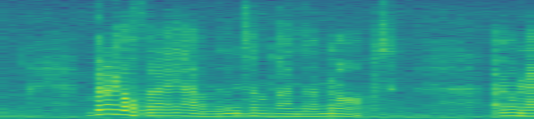
\includegraphics[interpolate=true,width=5.340000in,height=1.190000in]{spectrogram-img0.png}}%
\end{pgfscope}%
\begin{pgfscope}%
\pgfsetbuttcap%
\pgfsetroundjoin%
\definecolor{currentfill}{rgb}{0.000000,0.000000,0.000000}%
\pgfsetfillcolor{currentfill}%
\pgfsetlinewidth{0.803000pt}%
\definecolor{currentstroke}{rgb}{0.000000,0.000000,0.000000}%
\pgfsetstrokecolor{currentstroke}%
\pgfsetdash{}{0pt}%
\pgfsys@defobject{currentmarker}{\pgfqpoint{0.000000in}{-0.048611in}}{\pgfqpoint{0.000000in}{0.000000in}}{%
\pgfpathmoveto{\pgfqpoint{0.000000in}{0.000000in}}%
\pgfpathlineto{\pgfqpoint{0.000000in}{-0.048611in}}%
\pgfusepath{stroke,fill}%
}%
\begin{pgfscope}%
\pgfsys@transformshift{0.719445in}{0.565123in}%
\pgfsys@useobject{currentmarker}{}%
\end{pgfscope}%
\end{pgfscope}%
\begin{pgfscope}%
\definecolor{textcolor}{rgb}{0.000000,0.000000,0.000000}%
\pgfsetstrokecolor{textcolor}%
\pgfsetfillcolor{textcolor}%
\pgftext[x=0.719445in,y=0.467901in,,top]{\color{textcolor}\rmfamily\fontsize{10.000000}{12.000000}\selectfont \(\displaystyle {0.0}\)}%
\end{pgfscope}%
\begin{pgfscope}%
\pgfsetbuttcap%
\pgfsetroundjoin%
\definecolor{currentfill}{rgb}{0.000000,0.000000,0.000000}%
\pgfsetfillcolor{currentfill}%
\pgfsetlinewidth{0.803000pt}%
\definecolor{currentstroke}{rgb}{0.000000,0.000000,0.000000}%
\pgfsetstrokecolor{currentstroke}%
\pgfsetdash{}{0pt}%
\pgfsys@defobject{currentmarker}{\pgfqpoint{0.000000in}{-0.048611in}}{\pgfqpoint{0.000000in}{0.000000in}}{%
\pgfpathmoveto{\pgfqpoint{0.000000in}{0.000000in}}%
\pgfpathlineto{\pgfqpoint{0.000000in}{-0.048611in}}%
\pgfusepath{stroke,fill}%
}%
\begin{pgfscope}%
\pgfsys@transformshift{1.391390in}{0.565123in}%
\pgfsys@useobject{currentmarker}{}%
\end{pgfscope}%
\end{pgfscope}%
\begin{pgfscope}%
\definecolor{textcolor}{rgb}{0.000000,0.000000,0.000000}%
\pgfsetstrokecolor{textcolor}%
\pgfsetfillcolor{textcolor}%
\pgftext[x=1.391390in,y=0.467901in,,top]{\color{textcolor}\rmfamily\fontsize{10.000000}{12.000000}\selectfont \(\displaystyle {0.5}\)}%
\end{pgfscope}%
\begin{pgfscope}%
\pgfsetbuttcap%
\pgfsetroundjoin%
\definecolor{currentfill}{rgb}{0.000000,0.000000,0.000000}%
\pgfsetfillcolor{currentfill}%
\pgfsetlinewidth{0.803000pt}%
\definecolor{currentstroke}{rgb}{0.000000,0.000000,0.000000}%
\pgfsetstrokecolor{currentstroke}%
\pgfsetdash{}{0pt}%
\pgfsys@defobject{currentmarker}{\pgfqpoint{0.000000in}{-0.048611in}}{\pgfqpoint{0.000000in}{0.000000in}}{%
\pgfpathmoveto{\pgfqpoint{0.000000in}{0.000000in}}%
\pgfpathlineto{\pgfqpoint{0.000000in}{-0.048611in}}%
\pgfusepath{stroke,fill}%
}%
\begin{pgfscope}%
\pgfsys@transformshift{2.063335in}{0.565123in}%
\pgfsys@useobject{currentmarker}{}%
\end{pgfscope}%
\end{pgfscope}%
\begin{pgfscope}%
\definecolor{textcolor}{rgb}{0.000000,0.000000,0.000000}%
\pgfsetstrokecolor{textcolor}%
\pgfsetfillcolor{textcolor}%
\pgftext[x=2.063335in,y=0.467901in,,top]{\color{textcolor}\rmfamily\fontsize{10.000000}{12.000000}\selectfont \(\displaystyle {1.0}\)}%
\end{pgfscope}%
\begin{pgfscope}%
\pgfsetbuttcap%
\pgfsetroundjoin%
\definecolor{currentfill}{rgb}{0.000000,0.000000,0.000000}%
\pgfsetfillcolor{currentfill}%
\pgfsetlinewidth{0.803000pt}%
\definecolor{currentstroke}{rgb}{0.000000,0.000000,0.000000}%
\pgfsetstrokecolor{currentstroke}%
\pgfsetdash{}{0pt}%
\pgfsys@defobject{currentmarker}{\pgfqpoint{0.000000in}{-0.048611in}}{\pgfqpoint{0.000000in}{0.000000in}}{%
\pgfpathmoveto{\pgfqpoint{0.000000in}{0.000000in}}%
\pgfpathlineto{\pgfqpoint{0.000000in}{-0.048611in}}%
\pgfusepath{stroke,fill}%
}%
\begin{pgfscope}%
\pgfsys@transformshift{2.735280in}{0.565123in}%
\pgfsys@useobject{currentmarker}{}%
\end{pgfscope}%
\end{pgfscope}%
\begin{pgfscope}%
\definecolor{textcolor}{rgb}{0.000000,0.000000,0.000000}%
\pgfsetstrokecolor{textcolor}%
\pgfsetfillcolor{textcolor}%
\pgftext[x=2.735280in,y=0.467901in,,top]{\color{textcolor}\rmfamily\fontsize{10.000000}{12.000000}\selectfont \(\displaystyle {1.5}\)}%
\end{pgfscope}%
\begin{pgfscope}%
\pgfsetbuttcap%
\pgfsetroundjoin%
\definecolor{currentfill}{rgb}{0.000000,0.000000,0.000000}%
\pgfsetfillcolor{currentfill}%
\pgfsetlinewidth{0.803000pt}%
\definecolor{currentstroke}{rgb}{0.000000,0.000000,0.000000}%
\pgfsetstrokecolor{currentstroke}%
\pgfsetdash{}{0pt}%
\pgfsys@defobject{currentmarker}{\pgfqpoint{0.000000in}{-0.048611in}}{\pgfqpoint{0.000000in}{0.000000in}}{%
\pgfpathmoveto{\pgfqpoint{0.000000in}{0.000000in}}%
\pgfpathlineto{\pgfqpoint{0.000000in}{-0.048611in}}%
\pgfusepath{stroke,fill}%
}%
\begin{pgfscope}%
\pgfsys@transformshift{3.407225in}{0.565123in}%
\pgfsys@useobject{currentmarker}{}%
\end{pgfscope}%
\end{pgfscope}%
\begin{pgfscope}%
\definecolor{textcolor}{rgb}{0.000000,0.000000,0.000000}%
\pgfsetstrokecolor{textcolor}%
\pgfsetfillcolor{textcolor}%
\pgftext[x=3.407225in,y=0.467901in,,top]{\color{textcolor}\rmfamily\fontsize{10.000000}{12.000000}\selectfont \(\displaystyle {2.0}\)}%
\end{pgfscope}%
\begin{pgfscope}%
\pgfsetbuttcap%
\pgfsetroundjoin%
\definecolor{currentfill}{rgb}{0.000000,0.000000,0.000000}%
\pgfsetfillcolor{currentfill}%
\pgfsetlinewidth{0.803000pt}%
\definecolor{currentstroke}{rgb}{0.000000,0.000000,0.000000}%
\pgfsetstrokecolor{currentstroke}%
\pgfsetdash{}{0pt}%
\pgfsys@defobject{currentmarker}{\pgfqpoint{0.000000in}{-0.048611in}}{\pgfqpoint{0.000000in}{0.000000in}}{%
\pgfpathmoveto{\pgfqpoint{0.000000in}{0.000000in}}%
\pgfpathlineto{\pgfqpoint{0.000000in}{-0.048611in}}%
\pgfusepath{stroke,fill}%
}%
\begin{pgfscope}%
\pgfsys@transformshift{4.079170in}{0.565123in}%
\pgfsys@useobject{currentmarker}{}%
\end{pgfscope}%
\end{pgfscope}%
\begin{pgfscope}%
\definecolor{textcolor}{rgb}{0.000000,0.000000,0.000000}%
\pgfsetstrokecolor{textcolor}%
\pgfsetfillcolor{textcolor}%
\pgftext[x=4.079170in,y=0.467901in,,top]{\color{textcolor}\rmfamily\fontsize{10.000000}{12.000000}\selectfont \(\displaystyle {2.5}\)}%
\end{pgfscope}%
\begin{pgfscope}%
\pgfsetbuttcap%
\pgfsetroundjoin%
\definecolor{currentfill}{rgb}{0.000000,0.000000,0.000000}%
\pgfsetfillcolor{currentfill}%
\pgfsetlinewidth{0.803000pt}%
\definecolor{currentstroke}{rgb}{0.000000,0.000000,0.000000}%
\pgfsetstrokecolor{currentstroke}%
\pgfsetdash{}{0pt}%
\pgfsys@defobject{currentmarker}{\pgfqpoint{0.000000in}{-0.048611in}}{\pgfqpoint{0.000000in}{0.000000in}}{%
\pgfpathmoveto{\pgfqpoint{0.000000in}{0.000000in}}%
\pgfpathlineto{\pgfqpoint{0.000000in}{-0.048611in}}%
\pgfusepath{stroke,fill}%
}%
\begin{pgfscope}%
\pgfsys@transformshift{4.751115in}{0.565123in}%
\pgfsys@useobject{currentmarker}{}%
\end{pgfscope}%
\end{pgfscope}%
\begin{pgfscope}%
\definecolor{textcolor}{rgb}{0.000000,0.000000,0.000000}%
\pgfsetstrokecolor{textcolor}%
\pgfsetfillcolor{textcolor}%
\pgftext[x=4.751115in,y=0.467901in,,top]{\color{textcolor}\rmfamily\fontsize{10.000000}{12.000000}\selectfont \(\displaystyle {3.0}\)}%
\end{pgfscope}%
\begin{pgfscope}%
\pgfsetbuttcap%
\pgfsetroundjoin%
\definecolor{currentfill}{rgb}{0.000000,0.000000,0.000000}%
\pgfsetfillcolor{currentfill}%
\pgfsetlinewidth{0.803000pt}%
\definecolor{currentstroke}{rgb}{0.000000,0.000000,0.000000}%
\pgfsetstrokecolor{currentstroke}%
\pgfsetdash{}{0pt}%
\pgfsys@defobject{currentmarker}{\pgfqpoint{0.000000in}{-0.048611in}}{\pgfqpoint{0.000000in}{0.000000in}}{%
\pgfpathmoveto{\pgfqpoint{0.000000in}{0.000000in}}%
\pgfpathlineto{\pgfqpoint{0.000000in}{-0.048611in}}%
\pgfusepath{stroke,fill}%
}%
\begin{pgfscope}%
\pgfsys@transformshift{5.423060in}{0.565123in}%
\pgfsys@useobject{currentmarker}{}%
\end{pgfscope}%
\end{pgfscope}%
\begin{pgfscope}%
\definecolor{textcolor}{rgb}{0.000000,0.000000,0.000000}%
\pgfsetstrokecolor{textcolor}%
\pgfsetfillcolor{textcolor}%
\pgftext[x=5.423060in,y=0.467901in,,top]{\color{textcolor}\rmfamily\fontsize{10.000000}{12.000000}\selectfont \(\displaystyle {3.5}\)}%
\end{pgfscope}%
\begin{pgfscope}%
\definecolor{textcolor}{rgb}{0.000000,0.000000,0.000000}%
\pgfsetstrokecolor{textcolor}%
\pgfsetfillcolor{textcolor}%
\pgftext[x=3.385723in,y=0.288889in,,top]{\color{textcolor}\rmfamily\fontsize{10.000000}{12.000000}\selectfont Time (s)}%
\end{pgfscope}%
\begin{pgfscope}%
\pgfsetbuttcap%
\pgfsetroundjoin%
\definecolor{currentfill}{rgb}{0.000000,0.000000,0.000000}%
\pgfsetfillcolor{currentfill}%
\pgfsetlinewidth{0.803000pt}%
\definecolor{currentstroke}{rgb}{0.000000,0.000000,0.000000}%
\pgfsetstrokecolor{currentstroke}%
\pgfsetdash{}{0pt}%
\pgfsys@defobject{currentmarker}{\pgfqpoint{-0.048611in}{0.000000in}}{\pgfqpoint{0.000000in}{0.000000in}}{%
\pgfpathmoveto{\pgfqpoint{0.000000in}{0.000000in}}%
\pgfpathlineto{\pgfqpoint{-0.048611in}{0.000000in}}%
\pgfusepath{stroke,fill}%
}%
\begin{pgfscope}%
\pgfsys@transformshift{0.719445in}{0.565123in}%
\pgfsys@useobject{currentmarker}{}%
\end{pgfscope}%
\end{pgfscope}%
\begin{pgfscope}%
\definecolor{textcolor}{rgb}{0.000000,0.000000,0.000000}%
\pgfsetstrokecolor{textcolor}%
\pgfsetfillcolor{textcolor}%
\pgftext[x=0.552778in, y=0.516898in, left, base]{\color{textcolor}\rmfamily\fontsize{10.000000}{12.000000}\selectfont \(\displaystyle {0}\)}%
\end{pgfscope}%
\begin{pgfscope}%
\pgfsetbuttcap%
\pgfsetroundjoin%
\definecolor{currentfill}{rgb}{0.000000,0.000000,0.000000}%
\pgfsetfillcolor{currentfill}%
\pgfsetlinewidth{0.803000pt}%
\definecolor{currentstroke}{rgb}{0.000000,0.000000,0.000000}%
\pgfsetstrokecolor{currentstroke}%
\pgfsetdash{}{0pt}%
\pgfsys@defobject{currentmarker}{\pgfqpoint{-0.048611in}{0.000000in}}{\pgfqpoint{0.000000in}{0.000000in}}{%
\pgfpathmoveto{\pgfqpoint{0.000000in}{0.000000in}}%
\pgfpathlineto{\pgfqpoint{-0.048611in}{0.000000in}}%
\pgfusepath{stroke,fill}%
}%
\begin{pgfscope}%
\pgfsys@transformshift{0.719445in}{0.860870in}%
\pgfsys@useobject{currentmarker}{}%
\end{pgfscope}%
\end{pgfscope}%
\begin{pgfscope}%
\definecolor{textcolor}{rgb}{0.000000,0.000000,0.000000}%
\pgfsetstrokecolor{textcolor}%
\pgfsetfillcolor{textcolor}%
\pgftext[x=0.344444in, y=0.812645in, left, base]{\color{textcolor}\rmfamily\fontsize{10.000000}{12.000000}\selectfont \(\displaystyle {2000}\)}%
\end{pgfscope}%
\begin{pgfscope}%
\pgfsetbuttcap%
\pgfsetroundjoin%
\definecolor{currentfill}{rgb}{0.000000,0.000000,0.000000}%
\pgfsetfillcolor{currentfill}%
\pgfsetlinewidth{0.803000pt}%
\definecolor{currentstroke}{rgb}{0.000000,0.000000,0.000000}%
\pgfsetstrokecolor{currentstroke}%
\pgfsetdash{}{0pt}%
\pgfsys@defobject{currentmarker}{\pgfqpoint{-0.048611in}{0.000000in}}{\pgfqpoint{0.000000in}{0.000000in}}{%
\pgfpathmoveto{\pgfqpoint{0.000000in}{0.000000in}}%
\pgfpathlineto{\pgfqpoint{-0.048611in}{0.000000in}}%
\pgfusepath{stroke,fill}%
}%
\begin{pgfscope}%
\pgfsys@transformshift{0.719445in}{1.156616in}%
\pgfsys@useobject{currentmarker}{}%
\end{pgfscope}%
\end{pgfscope}%
\begin{pgfscope}%
\definecolor{textcolor}{rgb}{0.000000,0.000000,0.000000}%
\pgfsetstrokecolor{textcolor}%
\pgfsetfillcolor{textcolor}%
\pgftext[x=0.344444in, y=1.108391in, left, base]{\color{textcolor}\rmfamily\fontsize{10.000000}{12.000000}\selectfont \(\displaystyle {4000}\)}%
\end{pgfscope}%
\begin{pgfscope}%
\pgfsetbuttcap%
\pgfsetroundjoin%
\definecolor{currentfill}{rgb}{0.000000,0.000000,0.000000}%
\pgfsetfillcolor{currentfill}%
\pgfsetlinewidth{0.803000pt}%
\definecolor{currentstroke}{rgb}{0.000000,0.000000,0.000000}%
\pgfsetstrokecolor{currentstroke}%
\pgfsetdash{}{0pt}%
\pgfsys@defobject{currentmarker}{\pgfqpoint{-0.048611in}{0.000000in}}{\pgfqpoint{0.000000in}{0.000000in}}{%
\pgfpathmoveto{\pgfqpoint{0.000000in}{0.000000in}}%
\pgfpathlineto{\pgfqpoint{-0.048611in}{0.000000in}}%
\pgfusepath{stroke,fill}%
}%
\begin{pgfscope}%
\pgfsys@transformshift{0.719445in}{1.452363in}%
\pgfsys@useobject{currentmarker}{}%
\end{pgfscope}%
\end{pgfscope}%
\begin{pgfscope}%
\definecolor{textcolor}{rgb}{0.000000,0.000000,0.000000}%
\pgfsetstrokecolor{textcolor}%
\pgfsetfillcolor{textcolor}%
\pgftext[x=0.344444in, y=1.404138in, left, base]{\color{textcolor}\rmfamily\fontsize{10.000000}{12.000000}\selectfont \(\displaystyle {6000}\)}%
\end{pgfscope}%
\begin{pgfscope}%
\pgfsetbuttcap%
\pgfsetroundjoin%
\definecolor{currentfill}{rgb}{0.000000,0.000000,0.000000}%
\pgfsetfillcolor{currentfill}%
\pgfsetlinewidth{0.803000pt}%
\definecolor{currentstroke}{rgb}{0.000000,0.000000,0.000000}%
\pgfsetstrokecolor{currentstroke}%
\pgfsetdash{}{0pt}%
\pgfsys@defobject{currentmarker}{\pgfqpoint{-0.048611in}{0.000000in}}{\pgfqpoint{0.000000in}{0.000000in}}{%
\pgfpathmoveto{\pgfqpoint{0.000000in}{0.000000in}}%
\pgfpathlineto{\pgfqpoint{-0.048611in}{0.000000in}}%
\pgfusepath{stroke,fill}%
}%
\begin{pgfscope}%
\pgfsys@transformshift{0.719445in}{1.748110in}%
\pgfsys@useobject{currentmarker}{}%
\end{pgfscope}%
\end{pgfscope}%
\begin{pgfscope}%
\definecolor{textcolor}{rgb}{0.000000,0.000000,0.000000}%
\pgfsetstrokecolor{textcolor}%
\pgfsetfillcolor{textcolor}%
\pgftext[x=0.344444in, y=1.699884in, left, base]{\color{textcolor}\rmfamily\fontsize{10.000000}{12.000000}\selectfont \(\displaystyle {8000}\)}%
\end{pgfscope}%
\begin{pgfscope}%
\definecolor{textcolor}{rgb}{0.000000,0.000000,0.000000}%
\pgfsetstrokecolor{textcolor}%
\pgfsetfillcolor{textcolor}%
\pgftext[x=0.288889in,y=1.156616in,,bottom,rotate=90.000000]{\color{textcolor}\rmfamily\fontsize{10.000000}{12.000000}\selectfont Frequency (Hz)}%
\end{pgfscope}%
\begin{pgfscope}%
\pgfsetrectcap%
\pgfsetmiterjoin%
\pgfsetlinewidth{0.803000pt}%
\definecolor{currentstroke}{rgb}{0.000000,0.000000,0.000000}%
\pgfsetstrokecolor{currentstroke}%
\pgfsetdash{}{0pt}%
\pgfpathmoveto{\pgfqpoint{0.719445in}{0.565123in}}%
\pgfpathlineto{\pgfqpoint{0.719445in}{1.748110in}}%
\pgfusepath{stroke}%
\end{pgfscope}%
\begin{pgfscope}%
\pgfsetrectcap%
\pgfsetmiterjoin%
\pgfsetlinewidth{0.803000pt}%
\definecolor{currentstroke}{rgb}{0.000000,0.000000,0.000000}%
\pgfsetstrokecolor{currentstroke}%
\pgfsetdash{}{0pt}%
\pgfpathmoveto{\pgfqpoint{6.052000in}{0.565123in}}%
\pgfpathlineto{\pgfqpoint{6.052000in}{1.748110in}}%
\pgfusepath{stroke}%
\end{pgfscope}%
\begin{pgfscope}%
\pgfsetrectcap%
\pgfsetmiterjoin%
\pgfsetlinewidth{0.803000pt}%
\definecolor{currentstroke}{rgb}{0.000000,0.000000,0.000000}%
\pgfsetstrokecolor{currentstroke}%
\pgfsetdash{}{0pt}%
\pgfpathmoveto{\pgfqpoint{0.719445in}{0.565123in}}%
\pgfpathlineto{\pgfqpoint{6.052000in}{0.565123in}}%
\pgfusepath{stroke}%
\end{pgfscope}%
\begin{pgfscope}%
\pgfsetrectcap%
\pgfsetmiterjoin%
\pgfsetlinewidth{0.803000pt}%
\definecolor{currentstroke}{rgb}{0.000000,0.000000,0.000000}%
\pgfsetstrokecolor{currentstroke}%
\pgfsetdash{}{0pt}%
\pgfpathmoveto{\pgfqpoint{0.719445in}{1.748110in}}%
\pgfpathlineto{\pgfqpoint{6.052000in}{1.748110in}}%
\pgfusepath{stroke}%
\end{pgfscope}%
\end{pgfpicture}%
\makeatother%
\endgroup%

    \centering
    \caption[Spectrogram example]{\textbf{Top:} A 4 second audio signal sampled at 16kHz. \textbf{Bottom:} The spectrogram of the same signal created using STFT with no overlap and a window size of 1024.}
    \label{fig:spectrogram}
\end{figure}

In a discrete signal the number of Fourier coefficients, also called FFT-bins, is determined by the number of samples collected, while the frequency resolution of each bin is determined by the sampling rate of the signal and the number of bins. Equation \ref{eq:fft_tempresolution} and \ref{eq:fft_binresolution} show the relationship between the different parameters.

\begin{equation}\label{eq:fft_tempresolution}
    N = \frac{|x|}{2}
\end{equation}

\begin{equation}\label{eq:fft_binresolution}
    \Delta_{bin} = \frac{fs}{N}
\end{equation}

Here $N$ is the number of FFT-bins, $|x|$ is the number of samples. $\Delta_{bin}$ is the size per FFT-bin in Hz and $fs$ is the sampling rate of the signal in Hz. The smaller $N$ the better the time resolution. The smaller the bin size the better the frequency resolution. One can see that there always exists a trade-off between frequency resolution and time resolution. If we decrease the number of samples per frame of the \gls{stft} we get a better temporal resolution but therefore a worse frequency resolution. It is important to choose good parameters that fit the need of the task. The more exact frequency differentiation, the weaker the temporal differentiation becomes. For our task, a well-balanced resolution in both domains is required.

\section{Filters}

We make use of filters to create augmented views of the input data before feeding it into the neural network. Filters are one of the most important parts of \gls{dsp}. Their applications range from telecommunication to computer graphics \cite{FILTERSWEB07}. An abstract view of two of the most important types of filters, called \textit{low-pass} and \textit{high-pass} filters can be seen in Figure \ref{fig:lphp}. The frequencies in the passband are the ones that should not be altered by the filter while frequencies in the transition band should be linearly reduced and frequencies in the stopband should be removed entirely. As can be seen in Figure \ref{fig:lphp} a low-pass filter stops all frequencies above the transition band, while a high-pass filter stops all below it.

\begin{figure}[htbp]
    \centering
    %% Creator: Matplotlib, PGF backend
%%
%% To include the figure in your LaTeX document, write
%%   \input{<filename>.pgf}
%%
%% Make sure the required packages are loaded in your preamble
%%   \usepackage{pgf}
%%
%% and, on pdftex
%%   \usepackage[utf8]{inputenc}\DeclareUnicodeCharacter{2212}{-}
%%
%% or, on luatex and xetex
%%   \usepackage{unicode-math}
%%
%% Figures using additional raster images can only be included by \input if
%% they are in the same directory as the main LaTeX file. For loading figures
%% from other directories you can use the `import` package
%%   \usepackage{import}
%%
%% and then include the figures with
%%   \import{<path to file>}{<filename>.pgf}
%%
%% Matplotlib used the following preamble
%%
\begingroup%
\makeatletter%
\begin{pgfpicture}%
\pgfpathrectangle{\pgfpointorigin}{\pgfqpoint{6.202000in}{2.000000in}}%
\pgfusepath{use as bounding box, clip}%
\begin{pgfscope}%
\pgfsetbuttcap%
\pgfsetmiterjoin%
\definecolor{currentfill}{rgb}{1.000000,1.000000,1.000000}%
\pgfsetfillcolor{currentfill}%
\pgfsetlinewidth{0.000000pt}%
\definecolor{currentstroke}{rgb}{1.000000,1.000000,1.000000}%
\pgfsetstrokecolor{currentstroke}%
\pgfsetdash{}{0pt}%
\pgfpathmoveto{\pgfqpoint{0.000000in}{0.000000in}}%
\pgfpathlineto{\pgfqpoint{6.202000in}{0.000000in}}%
\pgfpathlineto{\pgfqpoint{6.202000in}{2.000000in}}%
\pgfpathlineto{\pgfqpoint{0.000000in}{2.000000in}}%
\pgfpathclose%
\pgfusepath{fill}%
\end{pgfscope}%
\begin{pgfscope}%
\pgfsetbuttcap%
\pgfsetmiterjoin%
\definecolor{currentfill}{rgb}{1.000000,1.000000,1.000000}%
\pgfsetfillcolor{currentfill}%
\pgfsetlinewidth{0.000000pt}%
\definecolor{currentstroke}{rgb}{0.000000,0.000000,0.000000}%
\pgfsetstrokecolor{currentstroke}%
\pgfsetstrokeopacity{0.000000}%
\pgfsetdash{}{0pt}%
\pgfpathmoveto{\pgfqpoint{0.329012in}{0.329012in}}%
\pgfpathlineto{\pgfqpoint{3.026000in}{0.329012in}}%
\pgfpathlineto{\pgfqpoint{3.026000in}{1.650926in}}%
\pgfpathlineto{\pgfqpoint{0.329012in}{1.650926in}}%
\pgfpathclose%
\pgfusepath{fill}%
\end{pgfscope}%
\begin{pgfscope}%
\definecolor{textcolor}{rgb}{0.000000,0.000000,0.000000}%
\pgfsetstrokecolor{textcolor}%
\pgfsetfillcolor{textcolor}%
\pgftext[x=1.677506in,y=0.273457in,,top]{\color{textcolor}\rmfamily\fontsize{10.000000}{12.000000}\selectfont Frequency}%
\end{pgfscope}%
\begin{pgfscope}%
\definecolor{textcolor}{rgb}{0.000000,0.000000,0.000000}%
\pgfsetstrokecolor{textcolor}%
\pgfsetfillcolor{textcolor}%
\pgftext[x=0.273457in,y=0.989969in,,bottom,rotate=90.000000]{\color{textcolor}\rmfamily\fontsize{10.000000}{12.000000}\selectfont Amplitude}%
\end{pgfscope}%
\begin{pgfscope}%
\pgfpathrectangle{\pgfqpoint{0.329012in}{0.329012in}}{\pgfqpoint{2.696988in}{1.321914in}}%
\pgfusepath{clip}%
\pgfsetbuttcap%
\pgfsetroundjoin%
\pgfsetlinewidth{1.505625pt}%
\definecolor{currentstroke}{rgb}{0.000000,0.000000,0.000000}%
\pgfsetstrokecolor{currentstroke}%
\pgfsetdash{{5.550000pt}{2.400000pt}}{0.000000pt}%
\pgfpathmoveto{\pgfqpoint{1.432325in}{0.319012in}}%
\pgfpathlineto{\pgfqpoint{1.432325in}{1.660926in}}%
\pgfusepath{stroke}%
\end{pgfscope}%
\begin{pgfscope}%
\pgfpathrectangle{\pgfqpoint{0.329012in}{0.329012in}}{\pgfqpoint{2.696988in}{1.321914in}}%
\pgfusepath{clip}%
\pgfsetbuttcap%
\pgfsetroundjoin%
\pgfsetlinewidth{1.505625pt}%
\definecolor{currentstroke}{rgb}{0.000000,0.000000,0.000000}%
\pgfsetstrokecolor{currentstroke}%
\pgfsetdash{{5.550000pt}{2.400000pt}}{0.000000pt}%
\pgfpathmoveto{\pgfqpoint{1.922687in}{0.319012in}}%
\pgfpathlineto{\pgfqpoint{1.922687in}{1.660926in}}%
\pgfusepath{stroke}%
\end{pgfscope}%
\begin{pgfscope}%
\pgfpathrectangle{\pgfqpoint{0.329012in}{0.329012in}}{\pgfqpoint{2.696988in}{1.321914in}}%
\pgfusepath{clip}%
\pgfsetrectcap%
\pgfsetroundjoin%
\pgfsetlinewidth{1.505625pt}%
\definecolor{currentstroke}{rgb}{0.121569,0.466667,0.705882}%
\pgfsetstrokecolor{currentstroke}%
\pgfsetdash{}{0pt}%
\pgfpathmoveto{\pgfqpoint{0.451603in}{1.530752in}}%
\pgfpathlineto{\pgfqpoint{1.432325in}{1.530752in}}%
\pgfpathlineto{\pgfqpoint{1.922687in}{0.329012in}}%
\pgfpathlineto{\pgfqpoint{2.903410in}{0.329012in}}%
\pgfusepath{stroke}%
\end{pgfscope}%
\begin{pgfscope}%
\pgfsetrectcap%
\pgfsetmiterjoin%
\pgfsetlinewidth{0.803000pt}%
\definecolor{currentstroke}{rgb}{0.000000,0.000000,0.000000}%
\pgfsetstrokecolor{currentstroke}%
\pgfsetdash{}{0pt}%
\pgfpathmoveto{\pgfqpoint{0.329012in}{0.329012in}}%
\pgfpathlineto{\pgfqpoint{0.329012in}{1.650926in}}%
\pgfusepath{stroke}%
\end{pgfscope}%
\begin{pgfscope}%
\pgfsetrectcap%
\pgfsetmiterjoin%
\pgfsetlinewidth{0.803000pt}%
\definecolor{currentstroke}{rgb}{0.000000,0.000000,0.000000}%
\pgfsetstrokecolor{currentstroke}%
\pgfsetdash{}{0pt}%
\pgfpathmoveto{\pgfqpoint{3.026000in}{0.329012in}}%
\pgfpathlineto{\pgfqpoint{3.026000in}{1.650926in}}%
\pgfusepath{stroke}%
\end{pgfscope}%
\begin{pgfscope}%
\pgfsetrectcap%
\pgfsetmiterjoin%
\pgfsetlinewidth{0.803000pt}%
\definecolor{currentstroke}{rgb}{0.000000,0.000000,0.000000}%
\pgfsetstrokecolor{currentstroke}%
\pgfsetdash{}{0pt}%
\pgfpathmoveto{\pgfqpoint{0.329012in}{0.329012in}}%
\pgfpathlineto{\pgfqpoint{3.026000in}{0.329012in}}%
\pgfusepath{stroke}%
\end{pgfscope}%
\begin{pgfscope}%
\pgfsetrectcap%
\pgfsetmiterjoin%
\pgfsetlinewidth{0.803000pt}%
\definecolor{currentstroke}{rgb}{0.000000,0.000000,0.000000}%
\pgfsetstrokecolor{currentstroke}%
\pgfsetdash{}{0pt}%
\pgfpathmoveto{\pgfqpoint{0.329012in}{1.650926in}}%
\pgfpathlineto{\pgfqpoint{3.026000in}{1.650926in}}%
\pgfusepath{stroke}%
\end{pgfscope}%
\begin{pgfscope}%
\definecolor{textcolor}{rgb}{0.000000,0.000000,0.000000}%
\pgfsetstrokecolor{textcolor}%
\pgfsetfillcolor{textcolor}%
\pgftext[x=0.451603in,y=1.350491in,left,base]{\color{textcolor}\rmfamily\fontsize{10.000000}{12.000000}\selectfont Passband}%
\end{pgfscope}%
\begin{pgfscope}%
\definecolor{textcolor}{rgb}{0.000000,0.000000,0.000000}%
\pgfsetstrokecolor{textcolor}%
\pgfsetfillcolor{textcolor}%
\pgftext[x=2.045277in,y=0.401117in,left,base]{\color{textcolor}\rmfamily\fontsize{10.000000}{12.000000}\selectfont Stopband}%
\end{pgfscope}%
\begin{pgfscope}%
\pgfsetroundcap%
\pgfsetroundjoin%
\pgfsetlinewidth{1.003750pt}%
\definecolor{currentstroke}{rgb}{0.000000,0.000000,0.000000}%
\pgfsetstrokecolor{currentstroke}%
\pgfsetdash{}{0pt}%
\pgfpathmoveto{\pgfqpoint{2.120600in}{1.034683in}}%
\pgfpathquadraticcurveto{\pgfqpoint{1.912562in}{0.985478in}}{\pgfqpoint{1.719635in}{0.939847in}}%
\pgfusepath{stroke}%
\end{pgfscope}%
\begin{pgfscope}%
\pgfsetroundcap%
\pgfsetroundjoin%
\pgfsetlinewidth{1.003750pt}%
\definecolor{currentstroke}{rgb}{0.000000,0.000000,0.000000}%
\pgfsetstrokecolor{currentstroke}%
\pgfsetdash{}{0pt}%
\pgfpathmoveto{\pgfqpoint{1.780092in}{0.925602in}}%
\pgfpathlineto{\pgfqpoint{1.719635in}{0.939847in}}%
\pgfpathlineto{\pgfqpoint{1.767305in}{0.979666in}}%
\pgfusepath{stroke}%
\end{pgfscope}%
\begin{pgfscope}%
\definecolor{textcolor}{rgb}{0.000000,0.000000,0.000000}%
\pgfsetstrokecolor{textcolor}%
\pgfsetfillcolor{textcolor}%
\pgftext[x=2.175452in, y=1.157901in, left, base]{\color{textcolor}\rmfamily\fontsize{10.000000}{12.000000}\selectfont Transition}%
\end{pgfscope}%
\begin{pgfscope}%
\definecolor{textcolor}{rgb}{0.000000,0.000000,0.000000}%
\pgfsetstrokecolor{textcolor}%
\pgfsetfillcolor{textcolor}%
\pgftext[x=2.336139in, y=1.015155in, left, base]{\color{textcolor}\rmfamily\fontsize{10.000000}{12.000000}\selectfont band}%
\end{pgfscope}%
\begin{pgfscope}%
\definecolor{textcolor}{rgb}{0.000000,0.000000,0.000000}%
\pgfsetstrokecolor{textcolor}%
\pgfsetfillcolor{textcolor}%
\pgftext[x=1.677506in,y=1.734260in,,base]{\color{textcolor}\rmfamily\fontsize{12.000000}{14.400000}\selectfont Low-pass Filter}%
\end{pgfscope}%
\begin{pgfscope}%
\pgfsetbuttcap%
\pgfsetmiterjoin%
\definecolor{currentfill}{rgb}{1.000000,1.000000,1.000000}%
\pgfsetfillcolor{currentfill}%
\pgfsetlinewidth{0.000000pt}%
\definecolor{currentstroke}{rgb}{0.000000,0.000000,0.000000}%
\pgfsetstrokecolor{currentstroke}%
\pgfsetstrokeopacity{0.000000}%
\pgfsetdash{}{0pt}%
\pgfpathmoveto{\pgfqpoint{3.355012in}{0.329012in}}%
\pgfpathlineto{\pgfqpoint{6.052000in}{0.329012in}}%
\pgfpathlineto{\pgfqpoint{6.052000in}{1.650926in}}%
\pgfpathlineto{\pgfqpoint{3.355012in}{1.650926in}}%
\pgfpathclose%
\pgfusepath{fill}%
\end{pgfscope}%
\begin{pgfscope}%
\definecolor{textcolor}{rgb}{0.000000,0.000000,0.000000}%
\pgfsetstrokecolor{textcolor}%
\pgfsetfillcolor{textcolor}%
\pgftext[x=4.703506in,y=0.273457in,,top]{\color{textcolor}\rmfamily\fontsize{10.000000}{12.000000}\selectfont Frequency}%
\end{pgfscope}%
\begin{pgfscope}%
\definecolor{textcolor}{rgb}{0.000000,0.000000,0.000000}%
\pgfsetstrokecolor{textcolor}%
\pgfsetfillcolor{textcolor}%
\pgftext[x=3.299457in,y=0.989969in,,bottom,rotate=90.000000]{\color{textcolor}\rmfamily\fontsize{10.000000}{12.000000}\selectfont Amplitude}%
\end{pgfscope}%
\begin{pgfscope}%
\pgfpathrectangle{\pgfqpoint{3.355012in}{0.329012in}}{\pgfqpoint{2.696988in}{1.321914in}}%
\pgfusepath{clip}%
\pgfsetrectcap%
\pgfsetroundjoin%
\pgfsetlinewidth{1.505625pt}%
\definecolor{currentstroke}{rgb}{0.121569,0.466667,0.705882}%
\pgfsetstrokecolor{currentstroke}%
\pgfsetdash{}{0pt}%
\pgfpathmoveto{\pgfqpoint{3.477603in}{0.329012in}}%
\pgfpathlineto{\pgfqpoint{4.458325in}{0.329012in}}%
\pgfpathlineto{\pgfqpoint{4.948687in}{1.530752in}}%
\pgfpathlineto{\pgfqpoint{5.929410in}{1.530752in}}%
\pgfusepath{stroke}%
\end{pgfscope}%
\begin{pgfscope}%
\pgfsetrectcap%
\pgfsetmiterjoin%
\pgfsetlinewidth{0.803000pt}%
\definecolor{currentstroke}{rgb}{0.000000,0.000000,0.000000}%
\pgfsetstrokecolor{currentstroke}%
\pgfsetdash{}{0pt}%
\pgfpathmoveto{\pgfqpoint{3.355012in}{0.329012in}}%
\pgfpathlineto{\pgfqpoint{3.355012in}{1.650926in}}%
\pgfusepath{stroke}%
\end{pgfscope}%
\begin{pgfscope}%
\pgfsetrectcap%
\pgfsetmiterjoin%
\pgfsetlinewidth{0.803000pt}%
\definecolor{currentstroke}{rgb}{0.000000,0.000000,0.000000}%
\pgfsetstrokecolor{currentstroke}%
\pgfsetdash{}{0pt}%
\pgfpathmoveto{\pgfqpoint{6.052000in}{0.329012in}}%
\pgfpathlineto{\pgfqpoint{6.052000in}{1.650926in}}%
\pgfusepath{stroke}%
\end{pgfscope}%
\begin{pgfscope}%
\pgfsetrectcap%
\pgfsetmiterjoin%
\pgfsetlinewidth{0.803000pt}%
\definecolor{currentstroke}{rgb}{0.000000,0.000000,0.000000}%
\pgfsetstrokecolor{currentstroke}%
\pgfsetdash{}{0pt}%
\pgfpathmoveto{\pgfqpoint{3.355012in}{0.329012in}}%
\pgfpathlineto{\pgfqpoint{6.052000in}{0.329012in}}%
\pgfusepath{stroke}%
\end{pgfscope}%
\begin{pgfscope}%
\pgfsetrectcap%
\pgfsetmiterjoin%
\pgfsetlinewidth{0.803000pt}%
\definecolor{currentstroke}{rgb}{0.000000,0.000000,0.000000}%
\pgfsetstrokecolor{currentstroke}%
\pgfsetdash{}{0pt}%
\pgfpathmoveto{\pgfqpoint{3.355012in}{1.650926in}}%
\pgfpathlineto{\pgfqpoint{6.052000in}{1.650926in}}%
\pgfusepath{stroke}%
\end{pgfscope}%
\begin{pgfscope}%
\definecolor{textcolor}{rgb}{0.000000,0.000000,0.000000}%
\pgfsetstrokecolor{textcolor}%
\pgfsetfillcolor{textcolor}%
\pgftext[x=4.703506in,y=1.734260in,,base]{\color{textcolor}\rmfamily\fontsize{12.000000}{14.400000}\selectfont High-pass Filter}%
\end{pgfscope}%
\end{pgfpicture}%
\makeatother%
\endgroup%

    \caption[]{\textbf{Left:} Abstract illustration of a \textit{low-pass} filter. \textbf{Right:} Abstract illustration of a \textit{high-pass} filter}
    \label{fig:lphp}
\end{figure}


Figure \ref{fig:filter_responses} shows how the same filter can be represented in time and in the frequency domain. The frequency response describes how the filter will affect the individual frequencies of an incoming signal. In this example, frequencies above 100Hz will be cut off linearly. The impulse response is the actual signal of the filter in the time domain. Applying a filter in the frequency domain can be achieved by multiplying an input’s frequency spectrum and the filter’s frequency response. It can be easily seen why multiplication will have the desired effect of removing all frequencies in the stopband while preserving all frequencies in the passband.

\begin{figure}[htbp]
    \centering
    %% Creator: Matplotlib, PGF backend
%%
%% To include the figure in your LaTeX document, write
%%   \input{<filename>.pgf}
%%
%% Make sure the required packages are loaded in your preamble
%%   \usepackage{pgf}
%%
%% and, on pdftex
%%   \usepackage[utf8]{inputenc}\DeclareUnicodeCharacter{2212}{-}
%%
%% or, on luatex and xetex
%%   \usepackage{unicode-math}
%%
%% Figures using additional raster images can only be included by \input if
%% they are in the same directory as the main LaTeX file. For loading figures
%% from other directories you can use the `import` package
%%   \usepackage{import}
%%
%% and then include the figures with
%%   \import{<path to file>}{<filename>.pgf}
%%
%% Matplotlib used the following preamble
%%
\begingroup%
\makeatletter%
\begin{pgfpicture}%
\pgfpathrectangle{\pgfpointorigin}{\pgfqpoint{6.202000in}{3.000000in}}%
\pgfusepath{use as bounding box, clip}%
\begin{pgfscope}%
\pgfsetbuttcap%
\pgfsetmiterjoin%
\definecolor{currentfill}{rgb}{1.000000,1.000000,1.000000}%
\pgfsetfillcolor{currentfill}%
\pgfsetlinewidth{0.000000pt}%
\definecolor{currentstroke}{rgb}{1.000000,1.000000,1.000000}%
\pgfsetstrokecolor{currentstroke}%
\pgfsetdash{}{0pt}%
\pgfpathmoveto{\pgfqpoint{0.000000in}{0.000000in}}%
\pgfpathlineto{\pgfqpoint{6.202000in}{0.000000in}}%
\pgfpathlineto{\pgfqpoint{6.202000in}{3.000000in}}%
\pgfpathlineto{\pgfqpoint{0.000000in}{3.000000in}}%
\pgfpathclose%
\pgfusepath{fill}%
\end{pgfscope}%
\begin{pgfscope}%
\pgfsetbuttcap%
\pgfsetmiterjoin%
\definecolor{currentfill}{rgb}{1.000000,1.000000,1.000000}%
\pgfsetfillcolor{currentfill}%
\pgfsetlinewidth{0.000000pt}%
\definecolor{currentstroke}{rgb}{0.000000,0.000000,0.000000}%
\pgfsetstrokecolor{currentstroke}%
\pgfsetstrokeopacity{0.000000}%
\pgfsetdash{}{0pt}%
\pgfpathmoveto{\pgfqpoint{0.688581in}{1.990123in}}%
\pgfpathlineto{\pgfqpoint{5.951402in}{1.990123in}}%
\pgfpathlineto{\pgfqpoint{5.951402in}{2.650926in}}%
\pgfpathlineto{\pgfqpoint{0.688581in}{2.650926in}}%
\pgfpathclose%
\pgfusepath{fill}%
\end{pgfscope}%
\begin{pgfscope}%
\pgfpathrectangle{\pgfqpoint{0.688581in}{1.990123in}}{\pgfqpoint{5.262821in}{0.660803in}}%
\pgfusepath{clip}%
\pgfsetrectcap%
\pgfsetroundjoin%
\pgfsetlinewidth{0.803000pt}%
\definecolor{currentstroke}{rgb}{0.690196,0.690196,0.690196}%
\pgfsetstrokecolor{currentstroke}%
\pgfsetdash{}{0pt}%
\pgfpathmoveto{\pgfqpoint{0.688581in}{1.990123in}}%
\pgfpathlineto{\pgfqpoint{0.688581in}{2.650926in}}%
\pgfusepath{stroke}%
\end{pgfscope}%
\begin{pgfscope}%
\pgfsetbuttcap%
\pgfsetroundjoin%
\definecolor{currentfill}{rgb}{0.000000,0.000000,0.000000}%
\pgfsetfillcolor{currentfill}%
\pgfsetlinewidth{0.803000pt}%
\definecolor{currentstroke}{rgb}{0.000000,0.000000,0.000000}%
\pgfsetstrokecolor{currentstroke}%
\pgfsetdash{}{0pt}%
\pgfsys@defobject{currentmarker}{\pgfqpoint{0.000000in}{-0.048611in}}{\pgfqpoint{0.000000in}{0.000000in}}{%
\pgfpathmoveto{\pgfqpoint{0.000000in}{0.000000in}}%
\pgfpathlineto{\pgfqpoint{0.000000in}{-0.048611in}}%
\pgfusepath{stroke,fill}%
}%
\begin{pgfscope}%
\pgfsys@transformshift{0.688581in}{1.990123in}%
\pgfsys@useobject{currentmarker}{}%
\end{pgfscope}%
\end{pgfscope}%
\begin{pgfscope}%
\definecolor{textcolor}{rgb}{0.000000,0.000000,0.000000}%
\pgfsetstrokecolor{textcolor}%
\pgfsetfillcolor{textcolor}%
\pgftext[x=0.688581in,y=1.892901in,,top]{\color{textcolor}\rmfamily\fontsize{10.000000}{12.000000}\selectfont \(\displaystyle {0.00}\)}%
\end{pgfscope}%
\begin{pgfscope}%
\pgfpathrectangle{\pgfqpoint{0.688581in}{1.990123in}}{\pgfqpoint{5.262821in}{0.660803in}}%
\pgfusepath{clip}%
\pgfsetrectcap%
\pgfsetroundjoin%
\pgfsetlinewidth{0.803000pt}%
\definecolor{currentstroke}{rgb}{0.690196,0.690196,0.690196}%
\pgfsetstrokecolor{currentstroke}%
\pgfsetdash{}{0pt}%
\pgfpathmoveto{\pgfqpoint{1.839435in}{1.990123in}}%
\pgfpathlineto{\pgfqpoint{1.839435in}{2.650926in}}%
\pgfusepath{stroke}%
\end{pgfscope}%
\begin{pgfscope}%
\pgfsetbuttcap%
\pgfsetroundjoin%
\definecolor{currentfill}{rgb}{0.000000,0.000000,0.000000}%
\pgfsetfillcolor{currentfill}%
\pgfsetlinewidth{0.803000pt}%
\definecolor{currentstroke}{rgb}{0.000000,0.000000,0.000000}%
\pgfsetstrokecolor{currentstroke}%
\pgfsetdash{}{0pt}%
\pgfsys@defobject{currentmarker}{\pgfqpoint{0.000000in}{-0.048611in}}{\pgfqpoint{0.000000in}{0.000000in}}{%
\pgfpathmoveto{\pgfqpoint{0.000000in}{0.000000in}}%
\pgfpathlineto{\pgfqpoint{0.000000in}{-0.048611in}}%
\pgfusepath{stroke,fill}%
}%
\begin{pgfscope}%
\pgfsys@transformshift{1.839435in}{1.990123in}%
\pgfsys@useobject{currentmarker}{}%
\end{pgfscope}%
\end{pgfscope}%
\begin{pgfscope}%
\definecolor{textcolor}{rgb}{0.000000,0.000000,0.000000}%
\pgfsetstrokecolor{textcolor}%
\pgfsetfillcolor{textcolor}%
\pgftext[x=1.839435in,y=1.892901in,,top]{\color{textcolor}\rmfamily\fontsize{10.000000}{12.000000}\selectfont \(\displaystyle {0.02}\)}%
\end{pgfscope}%
\begin{pgfscope}%
\pgfpathrectangle{\pgfqpoint{0.688581in}{1.990123in}}{\pgfqpoint{5.262821in}{0.660803in}}%
\pgfusepath{clip}%
\pgfsetrectcap%
\pgfsetroundjoin%
\pgfsetlinewidth{0.803000pt}%
\definecolor{currentstroke}{rgb}{0.690196,0.690196,0.690196}%
\pgfsetstrokecolor{currentstroke}%
\pgfsetdash{}{0pt}%
\pgfpathmoveto{\pgfqpoint{2.990289in}{1.990123in}}%
\pgfpathlineto{\pgfqpoint{2.990289in}{2.650926in}}%
\pgfusepath{stroke}%
\end{pgfscope}%
\begin{pgfscope}%
\pgfsetbuttcap%
\pgfsetroundjoin%
\definecolor{currentfill}{rgb}{0.000000,0.000000,0.000000}%
\pgfsetfillcolor{currentfill}%
\pgfsetlinewidth{0.803000pt}%
\definecolor{currentstroke}{rgb}{0.000000,0.000000,0.000000}%
\pgfsetstrokecolor{currentstroke}%
\pgfsetdash{}{0pt}%
\pgfsys@defobject{currentmarker}{\pgfqpoint{0.000000in}{-0.048611in}}{\pgfqpoint{0.000000in}{0.000000in}}{%
\pgfpathmoveto{\pgfqpoint{0.000000in}{0.000000in}}%
\pgfpathlineto{\pgfqpoint{0.000000in}{-0.048611in}}%
\pgfusepath{stroke,fill}%
}%
\begin{pgfscope}%
\pgfsys@transformshift{2.990289in}{1.990123in}%
\pgfsys@useobject{currentmarker}{}%
\end{pgfscope}%
\end{pgfscope}%
\begin{pgfscope}%
\definecolor{textcolor}{rgb}{0.000000,0.000000,0.000000}%
\pgfsetstrokecolor{textcolor}%
\pgfsetfillcolor{textcolor}%
\pgftext[x=2.990289in,y=1.892901in,,top]{\color{textcolor}\rmfamily\fontsize{10.000000}{12.000000}\selectfont \(\displaystyle {0.04}\)}%
\end{pgfscope}%
\begin{pgfscope}%
\pgfpathrectangle{\pgfqpoint{0.688581in}{1.990123in}}{\pgfqpoint{5.262821in}{0.660803in}}%
\pgfusepath{clip}%
\pgfsetrectcap%
\pgfsetroundjoin%
\pgfsetlinewidth{0.803000pt}%
\definecolor{currentstroke}{rgb}{0.690196,0.690196,0.690196}%
\pgfsetstrokecolor{currentstroke}%
\pgfsetdash{}{0pt}%
\pgfpathmoveto{\pgfqpoint{4.141143in}{1.990123in}}%
\pgfpathlineto{\pgfqpoint{4.141143in}{2.650926in}}%
\pgfusepath{stroke}%
\end{pgfscope}%
\begin{pgfscope}%
\pgfsetbuttcap%
\pgfsetroundjoin%
\definecolor{currentfill}{rgb}{0.000000,0.000000,0.000000}%
\pgfsetfillcolor{currentfill}%
\pgfsetlinewidth{0.803000pt}%
\definecolor{currentstroke}{rgb}{0.000000,0.000000,0.000000}%
\pgfsetstrokecolor{currentstroke}%
\pgfsetdash{}{0pt}%
\pgfsys@defobject{currentmarker}{\pgfqpoint{0.000000in}{-0.048611in}}{\pgfqpoint{0.000000in}{0.000000in}}{%
\pgfpathmoveto{\pgfqpoint{0.000000in}{0.000000in}}%
\pgfpathlineto{\pgfqpoint{0.000000in}{-0.048611in}}%
\pgfusepath{stroke,fill}%
}%
\begin{pgfscope}%
\pgfsys@transformshift{4.141143in}{1.990123in}%
\pgfsys@useobject{currentmarker}{}%
\end{pgfscope}%
\end{pgfscope}%
\begin{pgfscope}%
\definecolor{textcolor}{rgb}{0.000000,0.000000,0.000000}%
\pgfsetstrokecolor{textcolor}%
\pgfsetfillcolor{textcolor}%
\pgftext[x=4.141143in,y=1.892901in,,top]{\color{textcolor}\rmfamily\fontsize{10.000000}{12.000000}\selectfont \(\displaystyle {0.06}\)}%
\end{pgfscope}%
\begin{pgfscope}%
\pgfpathrectangle{\pgfqpoint{0.688581in}{1.990123in}}{\pgfqpoint{5.262821in}{0.660803in}}%
\pgfusepath{clip}%
\pgfsetrectcap%
\pgfsetroundjoin%
\pgfsetlinewidth{0.803000pt}%
\definecolor{currentstroke}{rgb}{0.690196,0.690196,0.690196}%
\pgfsetstrokecolor{currentstroke}%
\pgfsetdash{}{0pt}%
\pgfpathmoveto{\pgfqpoint{5.291996in}{1.990123in}}%
\pgfpathlineto{\pgfqpoint{5.291996in}{2.650926in}}%
\pgfusepath{stroke}%
\end{pgfscope}%
\begin{pgfscope}%
\pgfsetbuttcap%
\pgfsetroundjoin%
\definecolor{currentfill}{rgb}{0.000000,0.000000,0.000000}%
\pgfsetfillcolor{currentfill}%
\pgfsetlinewidth{0.803000pt}%
\definecolor{currentstroke}{rgb}{0.000000,0.000000,0.000000}%
\pgfsetstrokecolor{currentstroke}%
\pgfsetdash{}{0pt}%
\pgfsys@defobject{currentmarker}{\pgfqpoint{0.000000in}{-0.048611in}}{\pgfqpoint{0.000000in}{0.000000in}}{%
\pgfpathmoveto{\pgfqpoint{0.000000in}{0.000000in}}%
\pgfpathlineto{\pgfqpoint{0.000000in}{-0.048611in}}%
\pgfusepath{stroke,fill}%
}%
\begin{pgfscope}%
\pgfsys@transformshift{5.291996in}{1.990123in}%
\pgfsys@useobject{currentmarker}{}%
\end{pgfscope}%
\end{pgfscope}%
\begin{pgfscope}%
\definecolor{textcolor}{rgb}{0.000000,0.000000,0.000000}%
\pgfsetstrokecolor{textcolor}%
\pgfsetfillcolor{textcolor}%
\pgftext[x=5.291996in,y=1.892901in,,top]{\color{textcolor}\rmfamily\fontsize{10.000000}{12.000000}\selectfont \(\displaystyle {0.08}\)}%
\end{pgfscope}%
\begin{pgfscope}%
\definecolor{textcolor}{rgb}{0.000000,0.000000,0.000000}%
\pgfsetstrokecolor{textcolor}%
\pgfsetfillcolor{textcolor}%
\pgftext[x=3.319991in,y=1.713889in,,top]{\color{textcolor}\rmfamily\fontsize{10.000000}{12.000000}\selectfont Time (s)}%
\end{pgfscope}%
\begin{pgfscope}%
\pgfpathrectangle{\pgfqpoint{0.688581in}{1.990123in}}{\pgfqpoint{5.262821in}{0.660803in}}%
\pgfusepath{clip}%
\pgfsetrectcap%
\pgfsetroundjoin%
\pgfsetlinewidth{0.803000pt}%
\definecolor{currentstroke}{rgb}{0.690196,0.690196,0.690196}%
\pgfsetstrokecolor{currentstroke}%
\pgfsetdash{}{0pt}%
\pgfpathmoveto{\pgfqpoint{0.688581in}{2.110909in}}%
\pgfpathlineto{\pgfqpoint{5.951402in}{2.110909in}}%
\pgfusepath{stroke}%
\end{pgfscope}%
\begin{pgfscope}%
\pgfsetbuttcap%
\pgfsetroundjoin%
\definecolor{currentfill}{rgb}{0.000000,0.000000,0.000000}%
\pgfsetfillcolor{currentfill}%
\pgfsetlinewidth{0.803000pt}%
\definecolor{currentstroke}{rgb}{0.000000,0.000000,0.000000}%
\pgfsetstrokecolor{currentstroke}%
\pgfsetdash{}{0pt}%
\pgfsys@defobject{currentmarker}{\pgfqpoint{-0.048611in}{0.000000in}}{\pgfqpoint{0.000000in}{0.000000in}}{%
\pgfpathmoveto{\pgfqpoint{0.000000in}{0.000000in}}%
\pgfpathlineto{\pgfqpoint{-0.048611in}{0.000000in}}%
\pgfusepath{stroke,fill}%
}%
\begin{pgfscope}%
\pgfsys@transformshift{0.688581in}{2.110909in}%
\pgfsys@useobject{currentmarker}{}%
\end{pgfscope}%
\end{pgfscope}%
\begin{pgfscope}%
\definecolor{textcolor}{rgb}{0.000000,0.000000,0.000000}%
\pgfsetstrokecolor{textcolor}%
\pgfsetfillcolor{textcolor}%
\pgftext[x=0.521914in, y=2.062684in, left, base]{\color{textcolor}\rmfamily\fontsize{10.000000}{12.000000}\selectfont \(\displaystyle {0}\)}%
\end{pgfscope}%
\begin{pgfscope}%
\pgfpathrectangle{\pgfqpoint{0.688581in}{1.990123in}}{\pgfqpoint{5.262821in}{0.660803in}}%
\pgfusepath{clip}%
\pgfsetrectcap%
\pgfsetroundjoin%
\pgfsetlinewidth{0.803000pt}%
\definecolor{currentstroke}{rgb}{0.690196,0.690196,0.690196}%
\pgfsetstrokecolor{currentstroke}%
\pgfsetdash{}{0pt}%
\pgfpathmoveto{\pgfqpoint{0.688581in}{2.445417in}}%
\pgfpathlineto{\pgfqpoint{5.951402in}{2.445417in}}%
\pgfusepath{stroke}%
\end{pgfscope}%
\begin{pgfscope}%
\pgfsetbuttcap%
\pgfsetroundjoin%
\definecolor{currentfill}{rgb}{0.000000,0.000000,0.000000}%
\pgfsetfillcolor{currentfill}%
\pgfsetlinewidth{0.803000pt}%
\definecolor{currentstroke}{rgb}{0.000000,0.000000,0.000000}%
\pgfsetstrokecolor{currentstroke}%
\pgfsetdash{}{0pt}%
\pgfsys@defobject{currentmarker}{\pgfqpoint{-0.048611in}{0.000000in}}{\pgfqpoint{0.000000in}{0.000000in}}{%
\pgfpathmoveto{\pgfqpoint{0.000000in}{0.000000in}}%
\pgfpathlineto{\pgfqpoint{-0.048611in}{0.000000in}}%
\pgfusepath{stroke,fill}%
}%
\begin{pgfscope}%
\pgfsys@transformshift{0.688581in}{2.445417in}%
\pgfsys@useobject{currentmarker}{}%
\end{pgfscope}%
\end{pgfscope}%
\begin{pgfscope}%
\definecolor{textcolor}{rgb}{0.000000,0.000000,0.000000}%
\pgfsetstrokecolor{textcolor}%
\pgfsetfillcolor{textcolor}%
\pgftext[x=0.452469in, y=2.397192in, left, base]{\color{textcolor}\rmfamily\fontsize{10.000000}{12.000000}\selectfont \(\displaystyle {50}\)}%
\end{pgfscope}%
\begin{pgfscope}%
\definecolor{textcolor}{rgb}{0.000000,0.000000,0.000000}%
\pgfsetstrokecolor{textcolor}%
\pgfsetfillcolor{textcolor}%
\pgftext[x=0.396914in,y=2.320525in,,bottom,rotate=90.000000]{\color{textcolor}\rmfamily\fontsize{10.000000}{12.000000}\selectfont Amplitude}%
\end{pgfscope}%
\begin{pgfscope}%
\pgfpathrectangle{\pgfqpoint{0.688581in}{1.990123in}}{\pgfqpoint{5.262821in}{0.660803in}}%
\pgfusepath{clip}%
\pgfsetrectcap%
\pgfsetroundjoin%
\pgfsetlinewidth{1.505625pt}%
\definecolor{currentstroke}{rgb}{0.121569,0.466667,0.705882}%
\pgfsetstrokecolor{currentstroke}%
\pgfsetdash{}{0pt}%
\pgfpathmoveto{\pgfqpoint{0.688581in}{2.110909in}}%
\pgfpathlineto{\pgfqpoint{0.741741in}{2.112154in}}%
\pgfpathlineto{\pgfqpoint{0.794901in}{2.119696in}}%
\pgfpathlineto{\pgfqpoint{0.848060in}{2.136991in}}%
\pgfpathlineto{\pgfqpoint{0.901220in}{2.165104in}}%
\pgfpathlineto{\pgfqpoint{0.954380in}{2.203373in}}%
\pgfpathlineto{\pgfqpoint{1.007540in}{2.249976in}}%
\pgfpathlineto{\pgfqpoint{1.060700in}{2.302381in}}%
\pgfpathlineto{\pgfqpoint{1.113859in}{2.357722in}}%
\pgfpathlineto{\pgfqpoint{1.167019in}{2.413085in}}%
\pgfpathlineto{\pgfqpoint{1.220179in}{2.465725in}}%
\pgfpathlineto{\pgfqpoint{1.273339in}{2.513222in}}%
\pgfpathlineto{\pgfqpoint{1.326499in}{2.553581in}}%
\pgfpathlineto{\pgfqpoint{1.379658in}{2.585291in}}%
\pgfpathlineto{\pgfqpoint{1.432818in}{2.607346in}}%
\pgfpathlineto{\pgfqpoint{1.485978in}{2.619230in}}%
\pgfpathlineto{\pgfqpoint{1.539138in}{2.620890in}}%
\pgfpathlineto{\pgfqpoint{1.592298in}{2.612681in}}%
\pgfpathlineto{\pgfqpoint{1.645457in}{2.595309in}}%
\pgfpathlineto{\pgfqpoint{1.698617in}{2.569761in}}%
\pgfpathlineto{\pgfqpoint{1.751777in}{2.537236in}}%
\pgfpathlineto{\pgfqpoint{1.804937in}{2.499074in}}%
\pgfpathlineto{\pgfqpoint{1.858097in}{2.456690in}}%
\pgfpathlineto{\pgfqpoint{1.911256in}{2.411515in}}%
\pgfpathlineto{\pgfqpoint{1.964416in}{2.364939in}}%
\pgfpathlineto{\pgfqpoint{2.017576in}{2.318273in}}%
\pgfpathlineto{\pgfqpoint{2.070736in}{2.272704in}}%
\pgfpathlineto{\pgfqpoint{2.123896in}{2.229273in}}%
\pgfpathlineto{\pgfqpoint{2.177056in}{2.188855in}}%
\pgfpathlineto{\pgfqpoint{2.230215in}{2.152149in}}%
\pgfpathlineto{\pgfqpoint{2.283375in}{2.119672in}}%
\pgfpathlineto{\pgfqpoint{2.336535in}{2.091765in}}%
\pgfpathlineto{\pgfqpoint{2.389695in}{2.068600in}}%
\pgfpathlineto{\pgfqpoint{2.442855in}{2.050196in}}%
\pgfpathlineto{\pgfqpoint{2.496014in}{2.036433in}}%
\pgfpathlineto{\pgfqpoint{2.549174in}{2.027075in}}%
\pgfpathlineto{\pgfqpoint{2.602334in}{2.021787in}}%
\pgfpathlineto{\pgfqpoint{2.655494in}{2.020160in}}%
\pgfpathlineto{\pgfqpoint{2.708654in}{2.021728in}}%
\pgfpathlineto{\pgfqpoint{2.761813in}{2.025996in}}%
\pgfpathlineto{\pgfqpoint{2.814973in}{2.032449in}}%
\pgfpathlineto{\pgfqpoint{2.868133in}{2.040579in}}%
\pgfpathlineto{\pgfqpoint{2.921293in}{2.049895in}}%
\pgfpathlineto{\pgfqpoint{2.974453in}{2.059933in}}%
\pgfpathlineto{\pgfqpoint{3.027612in}{2.070273in}}%
\pgfpathlineto{\pgfqpoint{3.080772in}{2.080542in}}%
\pgfpathlineto{\pgfqpoint{3.133932in}{2.090418in}}%
\pgfpathlineto{\pgfqpoint{3.187092in}{2.099638in}}%
\pgfpathlineto{\pgfqpoint{3.240252in}{2.107993in}}%
\pgfpathlineto{\pgfqpoint{3.293411in}{2.115331in}}%
\pgfpathlineto{\pgfqpoint{3.346571in}{2.121553in}}%
\pgfpathlineto{\pgfqpoint{3.399731in}{2.126609in}}%
\pgfpathlineto{\pgfqpoint{3.452891in}{2.130491in}}%
\pgfpathlineto{\pgfqpoint{3.506051in}{2.133231in}}%
\pgfpathlineto{\pgfqpoint{3.559210in}{2.134895in}}%
\pgfpathlineto{\pgfqpoint{3.612370in}{2.135570in}}%
\pgfpathlineto{\pgfqpoint{3.665530in}{2.135367in}}%
\pgfpathlineto{\pgfqpoint{3.718690in}{2.134409in}}%
\pgfpathlineto{\pgfqpoint{3.771850in}{2.132827in}}%
\pgfpathlineto{\pgfqpoint{3.825009in}{2.130752in}}%
\pgfpathlineto{\pgfqpoint{3.878169in}{2.128317in}}%
\pgfpathlineto{\pgfqpoint{3.931329in}{2.125648in}}%
\pgfpathlineto{\pgfqpoint{3.984489in}{2.122859in}}%
\pgfpathlineto{\pgfqpoint{4.037649in}{2.120056in}}%
\pgfpathlineto{\pgfqpoint{4.090808in}{2.117330in}}%
\pgfpathlineto{\pgfqpoint{4.143968in}{2.114758in}}%
\pgfpathlineto{\pgfqpoint{4.197128in}{2.112401in}}%
\pgfpathlineto{\pgfqpoint{4.250288in}{2.110306in}}%
\pgfpathlineto{\pgfqpoint{4.303448in}{2.108505in}}%
\pgfpathlineto{\pgfqpoint{4.356608in}{2.107017in}}%
\pgfpathlineto{\pgfqpoint{4.409767in}{2.105848in}}%
\pgfpathlineto{\pgfqpoint{4.462927in}{2.104993in}}%
\pgfpathlineto{\pgfqpoint{4.516087in}{2.104438in}}%
\pgfpathlineto{\pgfqpoint{4.569247in}{2.104162in}}%
\pgfpathlineto{\pgfqpoint{4.622407in}{2.104135in}}%
\pgfpathlineto{\pgfqpoint{4.675566in}{2.104327in}}%
\pgfpathlineto{\pgfqpoint{4.728726in}{2.104702in}}%
\pgfpathlineto{\pgfqpoint{4.781886in}{2.105224in}}%
\pgfpathlineto{\pgfqpoint{4.835046in}{2.105858in}}%
\pgfpathlineto{\pgfqpoint{4.888206in}{2.106569in}}%
\pgfpathlineto{\pgfqpoint{4.941365in}{2.107323in}}%
\pgfpathlineto{\pgfqpoint{4.994525in}{2.108092in}}%
\pgfpathlineto{\pgfqpoint{5.047685in}{2.108849in}}%
\pgfpathlineto{\pgfqpoint{5.100845in}{2.109571in}}%
\pgfpathlineto{\pgfqpoint{5.154005in}{2.110240in}}%
\pgfpathlineto{\pgfqpoint{5.207164in}{2.110843in}}%
\pgfpathlineto{\pgfqpoint{5.260324in}{2.111368in}}%
\pgfpathlineto{\pgfqpoint{5.313484in}{2.111809in}}%
\pgfpathlineto{\pgfqpoint{5.366644in}{2.112164in}}%
\pgfpathlineto{\pgfqpoint{5.419804in}{2.112432in}}%
\pgfpathlineto{\pgfqpoint{5.472963in}{2.112616in}}%
\pgfpathlineto{\pgfqpoint{5.526123in}{2.112722in}}%
\pgfpathlineto{\pgfqpoint{5.579283in}{2.112756in}}%
\pgfpathlineto{\pgfqpoint{5.632443in}{2.112727in}}%
\pgfpathlineto{\pgfqpoint{5.685603in}{2.112644in}}%
\pgfpathlineto{\pgfqpoint{5.738762in}{2.112517in}}%
\pgfpathlineto{\pgfqpoint{5.791922in}{2.112356in}}%
\pgfpathlineto{\pgfqpoint{5.845082in}{2.112170in}}%
\pgfpathlineto{\pgfqpoint{5.898242in}{2.111969in}}%
\pgfpathlineto{\pgfqpoint{5.951402in}{2.111760in}}%
\pgfusepath{stroke}%
\end{pgfscope}%
\begin{pgfscope}%
\pgfsetrectcap%
\pgfsetmiterjoin%
\pgfsetlinewidth{0.803000pt}%
\definecolor{currentstroke}{rgb}{0.000000,0.000000,0.000000}%
\pgfsetstrokecolor{currentstroke}%
\pgfsetdash{}{0pt}%
\pgfpathmoveto{\pgfqpoint{0.688581in}{1.990123in}}%
\pgfpathlineto{\pgfqpoint{0.688581in}{2.650926in}}%
\pgfusepath{stroke}%
\end{pgfscope}%
\begin{pgfscope}%
\pgfsetrectcap%
\pgfsetmiterjoin%
\pgfsetlinewidth{0.803000pt}%
\definecolor{currentstroke}{rgb}{0.000000,0.000000,0.000000}%
\pgfsetstrokecolor{currentstroke}%
\pgfsetdash{}{0pt}%
\pgfpathmoveto{\pgfqpoint{5.951402in}{1.990123in}}%
\pgfpathlineto{\pgfqpoint{5.951402in}{2.650926in}}%
\pgfusepath{stroke}%
\end{pgfscope}%
\begin{pgfscope}%
\pgfsetrectcap%
\pgfsetmiterjoin%
\pgfsetlinewidth{0.803000pt}%
\definecolor{currentstroke}{rgb}{0.000000,0.000000,0.000000}%
\pgfsetstrokecolor{currentstroke}%
\pgfsetdash{}{0pt}%
\pgfpathmoveto{\pgfqpoint{0.688581in}{1.990123in}}%
\pgfpathlineto{\pgfqpoint{5.951402in}{1.990123in}}%
\pgfusepath{stroke}%
\end{pgfscope}%
\begin{pgfscope}%
\pgfsetrectcap%
\pgfsetmiterjoin%
\pgfsetlinewidth{0.803000pt}%
\definecolor{currentstroke}{rgb}{0.000000,0.000000,0.000000}%
\pgfsetstrokecolor{currentstroke}%
\pgfsetdash{}{0pt}%
\pgfpathmoveto{\pgfqpoint{0.688581in}{2.650926in}}%
\pgfpathlineto{\pgfqpoint{5.951402in}{2.650926in}}%
\pgfusepath{stroke}%
\end{pgfscope}%
\begin{pgfscope}%
\definecolor{textcolor}{rgb}{0.000000,0.000000,0.000000}%
\pgfsetstrokecolor{textcolor}%
\pgfsetfillcolor{textcolor}%
\pgftext[x=3.319991in,y=2.734260in,,base]{\color{textcolor}\rmfamily\fontsize{12.000000}{14.400000}\selectfont Impulse response}%
\end{pgfscope}%
\begin{pgfscope}%
\pgfsetbuttcap%
\pgfsetmiterjoin%
\definecolor{currentfill}{rgb}{1.000000,1.000000,1.000000}%
\pgfsetfillcolor{currentfill}%
\pgfsetlinewidth{0.000000pt}%
\definecolor{currentstroke}{rgb}{0.000000,0.000000,0.000000}%
\pgfsetstrokecolor{currentstroke}%
\pgfsetstrokeopacity{0.000000}%
\pgfsetdash{}{0pt}%
\pgfpathmoveto{\pgfqpoint{0.688581in}{0.565123in}}%
\pgfpathlineto{\pgfqpoint{5.951402in}{0.565123in}}%
\pgfpathlineto{\pgfqpoint{5.951402in}{1.225926in}}%
\pgfpathlineto{\pgfqpoint{0.688581in}{1.225926in}}%
\pgfpathclose%
\pgfusepath{fill}%
\end{pgfscope}%
\begin{pgfscope}%
\pgfpathrectangle{\pgfqpoint{0.688581in}{0.565123in}}{\pgfqpoint{5.262821in}{0.660803in}}%
\pgfusepath{clip}%
\pgfsetrectcap%
\pgfsetroundjoin%
\pgfsetlinewidth{0.803000pt}%
\definecolor{currentstroke}{rgb}{0.690196,0.690196,0.690196}%
\pgfsetstrokecolor{currentstroke}%
\pgfsetdash{}{0pt}%
\pgfpathmoveto{\pgfqpoint{0.688581in}{0.565123in}}%
\pgfpathlineto{\pgfqpoint{0.688581in}{1.225926in}}%
\pgfusepath{stroke}%
\end{pgfscope}%
\begin{pgfscope}%
\pgfsetbuttcap%
\pgfsetroundjoin%
\definecolor{currentfill}{rgb}{0.000000,0.000000,0.000000}%
\pgfsetfillcolor{currentfill}%
\pgfsetlinewidth{0.803000pt}%
\definecolor{currentstroke}{rgb}{0.000000,0.000000,0.000000}%
\pgfsetstrokecolor{currentstroke}%
\pgfsetdash{}{0pt}%
\pgfsys@defobject{currentmarker}{\pgfqpoint{0.000000in}{-0.048611in}}{\pgfqpoint{0.000000in}{0.000000in}}{%
\pgfpathmoveto{\pgfqpoint{0.000000in}{0.000000in}}%
\pgfpathlineto{\pgfqpoint{0.000000in}{-0.048611in}}%
\pgfusepath{stroke,fill}%
}%
\begin{pgfscope}%
\pgfsys@transformshift{0.688581in}{0.565123in}%
\pgfsys@useobject{currentmarker}{}%
\end{pgfscope}%
\end{pgfscope}%
\begin{pgfscope}%
\definecolor{textcolor}{rgb}{0.000000,0.000000,0.000000}%
\pgfsetstrokecolor{textcolor}%
\pgfsetfillcolor{textcolor}%
\pgftext[x=0.688581in,y=0.467901in,,top]{\color{textcolor}\rmfamily\fontsize{10.000000}{12.000000}\selectfont \(\displaystyle {10^{1}}\)}%
\end{pgfscope}%
\begin{pgfscope}%
\pgfpathrectangle{\pgfqpoint{0.688581in}{0.565123in}}{\pgfqpoint{5.262821in}{0.660803in}}%
\pgfusepath{clip}%
\pgfsetrectcap%
\pgfsetroundjoin%
\pgfsetlinewidth{0.803000pt}%
\definecolor{currentstroke}{rgb}{0.690196,0.690196,0.690196}%
\pgfsetstrokecolor{currentstroke}%
\pgfsetdash{}{0pt}%
\pgfpathmoveto{\pgfqpoint{3.319991in}{0.565123in}}%
\pgfpathlineto{\pgfqpoint{3.319991in}{1.225926in}}%
\pgfusepath{stroke}%
\end{pgfscope}%
\begin{pgfscope}%
\pgfsetbuttcap%
\pgfsetroundjoin%
\definecolor{currentfill}{rgb}{0.000000,0.000000,0.000000}%
\pgfsetfillcolor{currentfill}%
\pgfsetlinewidth{0.803000pt}%
\definecolor{currentstroke}{rgb}{0.000000,0.000000,0.000000}%
\pgfsetstrokecolor{currentstroke}%
\pgfsetdash{}{0pt}%
\pgfsys@defobject{currentmarker}{\pgfqpoint{0.000000in}{-0.048611in}}{\pgfqpoint{0.000000in}{0.000000in}}{%
\pgfpathmoveto{\pgfqpoint{0.000000in}{0.000000in}}%
\pgfpathlineto{\pgfqpoint{0.000000in}{-0.048611in}}%
\pgfusepath{stroke,fill}%
}%
\begin{pgfscope}%
\pgfsys@transformshift{3.319991in}{0.565123in}%
\pgfsys@useobject{currentmarker}{}%
\end{pgfscope}%
\end{pgfscope}%
\begin{pgfscope}%
\definecolor{textcolor}{rgb}{0.000000,0.000000,0.000000}%
\pgfsetstrokecolor{textcolor}%
\pgfsetfillcolor{textcolor}%
\pgftext[x=3.319991in,y=0.467901in,,top]{\color{textcolor}\rmfamily\fontsize{10.000000}{12.000000}\selectfont \(\displaystyle {10^{2}}\)}%
\end{pgfscope}%
\begin{pgfscope}%
\pgfpathrectangle{\pgfqpoint{0.688581in}{0.565123in}}{\pgfqpoint{5.262821in}{0.660803in}}%
\pgfusepath{clip}%
\pgfsetrectcap%
\pgfsetroundjoin%
\pgfsetlinewidth{0.803000pt}%
\definecolor{currentstroke}{rgb}{0.690196,0.690196,0.690196}%
\pgfsetstrokecolor{currentstroke}%
\pgfsetdash{}{0pt}%
\pgfpathmoveto{\pgfqpoint{5.951402in}{0.565123in}}%
\pgfpathlineto{\pgfqpoint{5.951402in}{1.225926in}}%
\pgfusepath{stroke}%
\end{pgfscope}%
\begin{pgfscope}%
\pgfsetbuttcap%
\pgfsetroundjoin%
\definecolor{currentfill}{rgb}{0.000000,0.000000,0.000000}%
\pgfsetfillcolor{currentfill}%
\pgfsetlinewidth{0.803000pt}%
\definecolor{currentstroke}{rgb}{0.000000,0.000000,0.000000}%
\pgfsetstrokecolor{currentstroke}%
\pgfsetdash{}{0pt}%
\pgfsys@defobject{currentmarker}{\pgfqpoint{0.000000in}{-0.048611in}}{\pgfqpoint{0.000000in}{0.000000in}}{%
\pgfpathmoveto{\pgfqpoint{0.000000in}{0.000000in}}%
\pgfpathlineto{\pgfqpoint{0.000000in}{-0.048611in}}%
\pgfusepath{stroke,fill}%
}%
\begin{pgfscope}%
\pgfsys@transformshift{5.951402in}{0.565123in}%
\pgfsys@useobject{currentmarker}{}%
\end{pgfscope}%
\end{pgfscope}%
\begin{pgfscope}%
\definecolor{textcolor}{rgb}{0.000000,0.000000,0.000000}%
\pgfsetstrokecolor{textcolor}%
\pgfsetfillcolor{textcolor}%
\pgftext[x=5.951402in,y=0.467901in,,top]{\color{textcolor}\rmfamily\fontsize{10.000000}{12.000000}\selectfont \(\displaystyle {10^{3}}\)}%
\end{pgfscope}%
\begin{pgfscope}%
\pgfpathrectangle{\pgfqpoint{0.688581in}{0.565123in}}{\pgfqpoint{5.262821in}{0.660803in}}%
\pgfusepath{clip}%
\pgfsetrectcap%
\pgfsetroundjoin%
\pgfsetlinewidth{0.803000pt}%
\definecolor{currentstroke}{rgb}{0.690196,0.690196,0.690196}%
\pgfsetstrokecolor{currentstroke}%
\pgfsetdash{}{0pt}%
\pgfpathmoveto{\pgfqpoint{1.480714in}{0.565123in}}%
\pgfpathlineto{\pgfqpoint{1.480714in}{1.225926in}}%
\pgfusepath{stroke}%
\end{pgfscope}%
\begin{pgfscope}%
\pgfsetbuttcap%
\pgfsetroundjoin%
\definecolor{currentfill}{rgb}{0.000000,0.000000,0.000000}%
\pgfsetfillcolor{currentfill}%
\pgfsetlinewidth{0.602250pt}%
\definecolor{currentstroke}{rgb}{0.000000,0.000000,0.000000}%
\pgfsetstrokecolor{currentstroke}%
\pgfsetdash{}{0pt}%
\pgfsys@defobject{currentmarker}{\pgfqpoint{0.000000in}{-0.027778in}}{\pgfqpoint{0.000000in}{0.000000in}}{%
\pgfpathmoveto{\pgfqpoint{0.000000in}{0.000000in}}%
\pgfpathlineto{\pgfqpoint{0.000000in}{-0.027778in}}%
\pgfusepath{stroke,fill}%
}%
\begin{pgfscope}%
\pgfsys@transformshift{1.480714in}{0.565123in}%
\pgfsys@useobject{currentmarker}{}%
\end{pgfscope}%
\end{pgfscope}%
\begin{pgfscope}%
\pgfpathrectangle{\pgfqpoint{0.688581in}{0.565123in}}{\pgfqpoint{5.262821in}{0.660803in}}%
\pgfusepath{clip}%
\pgfsetrectcap%
\pgfsetroundjoin%
\pgfsetlinewidth{0.803000pt}%
\definecolor{currentstroke}{rgb}{0.690196,0.690196,0.690196}%
\pgfsetstrokecolor{currentstroke}%
\pgfsetdash{}{0pt}%
\pgfpathmoveto{\pgfqpoint{1.944083in}{0.565123in}}%
\pgfpathlineto{\pgfqpoint{1.944083in}{1.225926in}}%
\pgfusepath{stroke}%
\end{pgfscope}%
\begin{pgfscope}%
\pgfsetbuttcap%
\pgfsetroundjoin%
\definecolor{currentfill}{rgb}{0.000000,0.000000,0.000000}%
\pgfsetfillcolor{currentfill}%
\pgfsetlinewidth{0.602250pt}%
\definecolor{currentstroke}{rgb}{0.000000,0.000000,0.000000}%
\pgfsetstrokecolor{currentstroke}%
\pgfsetdash{}{0pt}%
\pgfsys@defobject{currentmarker}{\pgfqpoint{0.000000in}{-0.027778in}}{\pgfqpoint{0.000000in}{0.000000in}}{%
\pgfpathmoveto{\pgfqpoint{0.000000in}{0.000000in}}%
\pgfpathlineto{\pgfqpoint{0.000000in}{-0.027778in}}%
\pgfusepath{stroke,fill}%
}%
\begin{pgfscope}%
\pgfsys@transformshift{1.944083in}{0.565123in}%
\pgfsys@useobject{currentmarker}{}%
\end{pgfscope}%
\end{pgfscope}%
\begin{pgfscope}%
\pgfpathrectangle{\pgfqpoint{0.688581in}{0.565123in}}{\pgfqpoint{5.262821in}{0.660803in}}%
\pgfusepath{clip}%
\pgfsetrectcap%
\pgfsetroundjoin%
\pgfsetlinewidth{0.803000pt}%
\definecolor{currentstroke}{rgb}{0.690196,0.690196,0.690196}%
\pgfsetstrokecolor{currentstroke}%
\pgfsetdash{}{0pt}%
\pgfpathmoveto{\pgfqpoint{2.272848in}{0.565123in}}%
\pgfpathlineto{\pgfqpoint{2.272848in}{1.225926in}}%
\pgfusepath{stroke}%
\end{pgfscope}%
\begin{pgfscope}%
\pgfsetbuttcap%
\pgfsetroundjoin%
\definecolor{currentfill}{rgb}{0.000000,0.000000,0.000000}%
\pgfsetfillcolor{currentfill}%
\pgfsetlinewidth{0.602250pt}%
\definecolor{currentstroke}{rgb}{0.000000,0.000000,0.000000}%
\pgfsetstrokecolor{currentstroke}%
\pgfsetdash{}{0pt}%
\pgfsys@defobject{currentmarker}{\pgfqpoint{0.000000in}{-0.027778in}}{\pgfqpoint{0.000000in}{0.000000in}}{%
\pgfpathmoveto{\pgfqpoint{0.000000in}{0.000000in}}%
\pgfpathlineto{\pgfqpoint{0.000000in}{-0.027778in}}%
\pgfusepath{stroke,fill}%
}%
\begin{pgfscope}%
\pgfsys@transformshift{2.272848in}{0.565123in}%
\pgfsys@useobject{currentmarker}{}%
\end{pgfscope}%
\end{pgfscope}%
\begin{pgfscope}%
\pgfpathrectangle{\pgfqpoint{0.688581in}{0.565123in}}{\pgfqpoint{5.262821in}{0.660803in}}%
\pgfusepath{clip}%
\pgfsetrectcap%
\pgfsetroundjoin%
\pgfsetlinewidth{0.803000pt}%
\definecolor{currentstroke}{rgb}{0.690196,0.690196,0.690196}%
\pgfsetstrokecolor{currentstroke}%
\pgfsetdash{}{0pt}%
\pgfpathmoveto{\pgfqpoint{2.527858in}{0.565123in}}%
\pgfpathlineto{\pgfqpoint{2.527858in}{1.225926in}}%
\pgfusepath{stroke}%
\end{pgfscope}%
\begin{pgfscope}%
\pgfsetbuttcap%
\pgfsetroundjoin%
\definecolor{currentfill}{rgb}{0.000000,0.000000,0.000000}%
\pgfsetfillcolor{currentfill}%
\pgfsetlinewidth{0.602250pt}%
\definecolor{currentstroke}{rgb}{0.000000,0.000000,0.000000}%
\pgfsetstrokecolor{currentstroke}%
\pgfsetdash{}{0pt}%
\pgfsys@defobject{currentmarker}{\pgfqpoint{0.000000in}{-0.027778in}}{\pgfqpoint{0.000000in}{0.000000in}}{%
\pgfpathmoveto{\pgfqpoint{0.000000in}{0.000000in}}%
\pgfpathlineto{\pgfqpoint{0.000000in}{-0.027778in}}%
\pgfusepath{stroke,fill}%
}%
\begin{pgfscope}%
\pgfsys@transformshift{2.527858in}{0.565123in}%
\pgfsys@useobject{currentmarker}{}%
\end{pgfscope}%
\end{pgfscope}%
\begin{pgfscope}%
\pgfpathrectangle{\pgfqpoint{0.688581in}{0.565123in}}{\pgfqpoint{5.262821in}{0.660803in}}%
\pgfusepath{clip}%
\pgfsetrectcap%
\pgfsetroundjoin%
\pgfsetlinewidth{0.803000pt}%
\definecolor{currentstroke}{rgb}{0.690196,0.690196,0.690196}%
\pgfsetstrokecolor{currentstroke}%
\pgfsetdash{}{0pt}%
\pgfpathmoveto{\pgfqpoint{2.736216in}{0.565123in}}%
\pgfpathlineto{\pgfqpoint{2.736216in}{1.225926in}}%
\pgfusepath{stroke}%
\end{pgfscope}%
\begin{pgfscope}%
\pgfsetbuttcap%
\pgfsetroundjoin%
\definecolor{currentfill}{rgb}{0.000000,0.000000,0.000000}%
\pgfsetfillcolor{currentfill}%
\pgfsetlinewidth{0.602250pt}%
\definecolor{currentstroke}{rgb}{0.000000,0.000000,0.000000}%
\pgfsetstrokecolor{currentstroke}%
\pgfsetdash{}{0pt}%
\pgfsys@defobject{currentmarker}{\pgfqpoint{0.000000in}{-0.027778in}}{\pgfqpoint{0.000000in}{0.000000in}}{%
\pgfpathmoveto{\pgfqpoint{0.000000in}{0.000000in}}%
\pgfpathlineto{\pgfqpoint{0.000000in}{-0.027778in}}%
\pgfusepath{stroke,fill}%
}%
\begin{pgfscope}%
\pgfsys@transformshift{2.736216in}{0.565123in}%
\pgfsys@useobject{currentmarker}{}%
\end{pgfscope}%
\end{pgfscope}%
\begin{pgfscope}%
\pgfpathrectangle{\pgfqpoint{0.688581in}{0.565123in}}{\pgfqpoint{5.262821in}{0.660803in}}%
\pgfusepath{clip}%
\pgfsetrectcap%
\pgfsetroundjoin%
\pgfsetlinewidth{0.803000pt}%
\definecolor{currentstroke}{rgb}{0.690196,0.690196,0.690196}%
\pgfsetstrokecolor{currentstroke}%
\pgfsetdash{}{0pt}%
\pgfpathmoveto{\pgfqpoint{2.912381in}{0.565123in}}%
\pgfpathlineto{\pgfqpoint{2.912381in}{1.225926in}}%
\pgfusepath{stroke}%
\end{pgfscope}%
\begin{pgfscope}%
\pgfsetbuttcap%
\pgfsetroundjoin%
\definecolor{currentfill}{rgb}{0.000000,0.000000,0.000000}%
\pgfsetfillcolor{currentfill}%
\pgfsetlinewidth{0.602250pt}%
\definecolor{currentstroke}{rgb}{0.000000,0.000000,0.000000}%
\pgfsetstrokecolor{currentstroke}%
\pgfsetdash{}{0pt}%
\pgfsys@defobject{currentmarker}{\pgfqpoint{0.000000in}{-0.027778in}}{\pgfqpoint{0.000000in}{0.000000in}}{%
\pgfpathmoveto{\pgfqpoint{0.000000in}{0.000000in}}%
\pgfpathlineto{\pgfqpoint{0.000000in}{-0.027778in}}%
\pgfusepath{stroke,fill}%
}%
\begin{pgfscope}%
\pgfsys@transformshift{2.912381in}{0.565123in}%
\pgfsys@useobject{currentmarker}{}%
\end{pgfscope}%
\end{pgfscope}%
\begin{pgfscope}%
\pgfpathrectangle{\pgfqpoint{0.688581in}{0.565123in}}{\pgfqpoint{5.262821in}{0.660803in}}%
\pgfusepath{clip}%
\pgfsetrectcap%
\pgfsetroundjoin%
\pgfsetlinewidth{0.803000pt}%
\definecolor{currentstroke}{rgb}{0.690196,0.690196,0.690196}%
\pgfsetstrokecolor{currentstroke}%
\pgfsetdash{}{0pt}%
\pgfpathmoveto{\pgfqpoint{3.064981in}{0.565123in}}%
\pgfpathlineto{\pgfqpoint{3.064981in}{1.225926in}}%
\pgfusepath{stroke}%
\end{pgfscope}%
\begin{pgfscope}%
\pgfsetbuttcap%
\pgfsetroundjoin%
\definecolor{currentfill}{rgb}{0.000000,0.000000,0.000000}%
\pgfsetfillcolor{currentfill}%
\pgfsetlinewidth{0.602250pt}%
\definecolor{currentstroke}{rgb}{0.000000,0.000000,0.000000}%
\pgfsetstrokecolor{currentstroke}%
\pgfsetdash{}{0pt}%
\pgfsys@defobject{currentmarker}{\pgfqpoint{0.000000in}{-0.027778in}}{\pgfqpoint{0.000000in}{0.000000in}}{%
\pgfpathmoveto{\pgfqpoint{0.000000in}{0.000000in}}%
\pgfpathlineto{\pgfqpoint{0.000000in}{-0.027778in}}%
\pgfusepath{stroke,fill}%
}%
\begin{pgfscope}%
\pgfsys@transformshift{3.064981in}{0.565123in}%
\pgfsys@useobject{currentmarker}{}%
\end{pgfscope}%
\end{pgfscope}%
\begin{pgfscope}%
\pgfpathrectangle{\pgfqpoint{0.688581in}{0.565123in}}{\pgfqpoint{5.262821in}{0.660803in}}%
\pgfusepath{clip}%
\pgfsetrectcap%
\pgfsetroundjoin%
\pgfsetlinewidth{0.803000pt}%
\definecolor{currentstroke}{rgb}{0.690196,0.690196,0.690196}%
\pgfsetstrokecolor{currentstroke}%
\pgfsetdash{}{0pt}%
\pgfpathmoveto{\pgfqpoint{3.199585in}{0.565123in}}%
\pgfpathlineto{\pgfqpoint{3.199585in}{1.225926in}}%
\pgfusepath{stroke}%
\end{pgfscope}%
\begin{pgfscope}%
\pgfsetbuttcap%
\pgfsetroundjoin%
\definecolor{currentfill}{rgb}{0.000000,0.000000,0.000000}%
\pgfsetfillcolor{currentfill}%
\pgfsetlinewidth{0.602250pt}%
\definecolor{currentstroke}{rgb}{0.000000,0.000000,0.000000}%
\pgfsetstrokecolor{currentstroke}%
\pgfsetdash{}{0pt}%
\pgfsys@defobject{currentmarker}{\pgfqpoint{0.000000in}{-0.027778in}}{\pgfqpoint{0.000000in}{0.000000in}}{%
\pgfpathmoveto{\pgfqpoint{0.000000in}{0.000000in}}%
\pgfpathlineto{\pgfqpoint{0.000000in}{-0.027778in}}%
\pgfusepath{stroke,fill}%
}%
\begin{pgfscope}%
\pgfsys@transformshift{3.199585in}{0.565123in}%
\pgfsys@useobject{currentmarker}{}%
\end{pgfscope}%
\end{pgfscope}%
\begin{pgfscope}%
\pgfpathrectangle{\pgfqpoint{0.688581in}{0.565123in}}{\pgfqpoint{5.262821in}{0.660803in}}%
\pgfusepath{clip}%
\pgfsetrectcap%
\pgfsetroundjoin%
\pgfsetlinewidth{0.803000pt}%
\definecolor{currentstroke}{rgb}{0.690196,0.690196,0.690196}%
\pgfsetstrokecolor{currentstroke}%
\pgfsetdash{}{0pt}%
\pgfpathmoveto{\pgfqpoint{4.112125in}{0.565123in}}%
\pgfpathlineto{\pgfqpoint{4.112125in}{1.225926in}}%
\pgfusepath{stroke}%
\end{pgfscope}%
\begin{pgfscope}%
\pgfsetbuttcap%
\pgfsetroundjoin%
\definecolor{currentfill}{rgb}{0.000000,0.000000,0.000000}%
\pgfsetfillcolor{currentfill}%
\pgfsetlinewidth{0.602250pt}%
\definecolor{currentstroke}{rgb}{0.000000,0.000000,0.000000}%
\pgfsetstrokecolor{currentstroke}%
\pgfsetdash{}{0pt}%
\pgfsys@defobject{currentmarker}{\pgfqpoint{0.000000in}{-0.027778in}}{\pgfqpoint{0.000000in}{0.000000in}}{%
\pgfpathmoveto{\pgfqpoint{0.000000in}{0.000000in}}%
\pgfpathlineto{\pgfqpoint{0.000000in}{-0.027778in}}%
\pgfusepath{stroke,fill}%
}%
\begin{pgfscope}%
\pgfsys@transformshift{4.112125in}{0.565123in}%
\pgfsys@useobject{currentmarker}{}%
\end{pgfscope}%
\end{pgfscope}%
\begin{pgfscope}%
\pgfpathrectangle{\pgfqpoint{0.688581in}{0.565123in}}{\pgfqpoint{5.262821in}{0.660803in}}%
\pgfusepath{clip}%
\pgfsetrectcap%
\pgfsetroundjoin%
\pgfsetlinewidth{0.803000pt}%
\definecolor{currentstroke}{rgb}{0.690196,0.690196,0.690196}%
\pgfsetstrokecolor{currentstroke}%
\pgfsetdash{}{0pt}%
\pgfpathmoveto{\pgfqpoint{4.575493in}{0.565123in}}%
\pgfpathlineto{\pgfqpoint{4.575493in}{1.225926in}}%
\pgfusepath{stroke}%
\end{pgfscope}%
\begin{pgfscope}%
\pgfsetbuttcap%
\pgfsetroundjoin%
\definecolor{currentfill}{rgb}{0.000000,0.000000,0.000000}%
\pgfsetfillcolor{currentfill}%
\pgfsetlinewidth{0.602250pt}%
\definecolor{currentstroke}{rgb}{0.000000,0.000000,0.000000}%
\pgfsetstrokecolor{currentstroke}%
\pgfsetdash{}{0pt}%
\pgfsys@defobject{currentmarker}{\pgfqpoint{0.000000in}{-0.027778in}}{\pgfqpoint{0.000000in}{0.000000in}}{%
\pgfpathmoveto{\pgfqpoint{0.000000in}{0.000000in}}%
\pgfpathlineto{\pgfqpoint{0.000000in}{-0.027778in}}%
\pgfusepath{stroke,fill}%
}%
\begin{pgfscope}%
\pgfsys@transformshift{4.575493in}{0.565123in}%
\pgfsys@useobject{currentmarker}{}%
\end{pgfscope}%
\end{pgfscope}%
\begin{pgfscope}%
\pgfpathrectangle{\pgfqpoint{0.688581in}{0.565123in}}{\pgfqpoint{5.262821in}{0.660803in}}%
\pgfusepath{clip}%
\pgfsetrectcap%
\pgfsetroundjoin%
\pgfsetlinewidth{0.803000pt}%
\definecolor{currentstroke}{rgb}{0.690196,0.690196,0.690196}%
\pgfsetstrokecolor{currentstroke}%
\pgfsetdash{}{0pt}%
\pgfpathmoveto{\pgfqpoint{4.904258in}{0.565123in}}%
\pgfpathlineto{\pgfqpoint{4.904258in}{1.225926in}}%
\pgfusepath{stroke}%
\end{pgfscope}%
\begin{pgfscope}%
\pgfsetbuttcap%
\pgfsetroundjoin%
\definecolor{currentfill}{rgb}{0.000000,0.000000,0.000000}%
\pgfsetfillcolor{currentfill}%
\pgfsetlinewidth{0.602250pt}%
\definecolor{currentstroke}{rgb}{0.000000,0.000000,0.000000}%
\pgfsetstrokecolor{currentstroke}%
\pgfsetdash{}{0pt}%
\pgfsys@defobject{currentmarker}{\pgfqpoint{0.000000in}{-0.027778in}}{\pgfqpoint{0.000000in}{0.000000in}}{%
\pgfpathmoveto{\pgfqpoint{0.000000in}{0.000000in}}%
\pgfpathlineto{\pgfqpoint{0.000000in}{-0.027778in}}%
\pgfusepath{stroke,fill}%
}%
\begin{pgfscope}%
\pgfsys@transformshift{4.904258in}{0.565123in}%
\pgfsys@useobject{currentmarker}{}%
\end{pgfscope}%
\end{pgfscope}%
\begin{pgfscope}%
\pgfpathrectangle{\pgfqpoint{0.688581in}{0.565123in}}{\pgfqpoint{5.262821in}{0.660803in}}%
\pgfusepath{clip}%
\pgfsetrectcap%
\pgfsetroundjoin%
\pgfsetlinewidth{0.803000pt}%
\definecolor{currentstroke}{rgb}{0.690196,0.690196,0.690196}%
\pgfsetstrokecolor{currentstroke}%
\pgfsetdash{}{0pt}%
\pgfpathmoveto{\pgfqpoint{5.159268in}{0.565123in}}%
\pgfpathlineto{\pgfqpoint{5.159268in}{1.225926in}}%
\pgfusepath{stroke}%
\end{pgfscope}%
\begin{pgfscope}%
\pgfsetbuttcap%
\pgfsetroundjoin%
\definecolor{currentfill}{rgb}{0.000000,0.000000,0.000000}%
\pgfsetfillcolor{currentfill}%
\pgfsetlinewidth{0.602250pt}%
\definecolor{currentstroke}{rgb}{0.000000,0.000000,0.000000}%
\pgfsetstrokecolor{currentstroke}%
\pgfsetdash{}{0pt}%
\pgfsys@defobject{currentmarker}{\pgfqpoint{0.000000in}{-0.027778in}}{\pgfqpoint{0.000000in}{0.000000in}}{%
\pgfpathmoveto{\pgfqpoint{0.000000in}{0.000000in}}%
\pgfpathlineto{\pgfqpoint{0.000000in}{-0.027778in}}%
\pgfusepath{stroke,fill}%
}%
\begin{pgfscope}%
\pgfsys@transformshift{5.159268in}{0.565123in}%
\pgfsys@useobject{currentmarker}{}%
\end{pgfscope}%
\end{pgfscope}%
\begin{pgfscope}%
\pgfpathrectangle{\pgfqpoint{0.688581in}{0.565123in}}{\pgfqpoint{5.262821in}{0.660803in}}%
\pgfusepath{clip}%
\pgfsetrectcap%
\pgfsetroundjoin%
\pgfsetlinewidth{0.803000pt}%
\definecolor{currentstroke}{rgb}{0.690196,0.690196,0.690196}%
\pgfsetstrokecolor{currentstroke}%
\pgfsetdash{}{0pt}%
\pgfpathmoveto{\pgfqpoint{5.367627in}{0.565123in}}%
\pgfpathlineto{\pgfqpoint{5.367627in}{1.225926in}}%
\pgfusepath{stroke}%
\end{pgfscope}%
\begin{pgfscope}%
\pgfsetbuttcap%
\pgfsetroundjoin%
\definecolor{currentfill}{rgb}{0.000000,0.000000,0.000000}%
\pgfsetfillcolor{currentfill}%
\pgfsetlinewidth{0.602250pt}%
\definecolor{currentstroke}{rgb}{0.000000,0.000000,0.000000}%
\pgfsetstrokecolor{currentstroke}%
\pgfsetdash{}{0pt}%
\pgfsys@defobject{currentmarker}{\pgfqpoint{0.000000in}{-0.027778in}}{\pgfqpoint{0.000000in}{0.000000in}}{%
\pgfpathmoveto{\pgfqpoint{0.000000in}{0.000000in}}%
\pgfpathlineto{\pgfqpoint{0.000000in}{-0.027778in}}%
\pgfusepath{stroke,fill}%
}%
\begin{pgfscope}%
\pgfsys@transformshift{5.367627in}{0.565123in}%
\pgfsys@useobject{currentmarker}{}%
\end{pgfscope}%
\end{pgfscope}%
\begin{pgfscope}%
\pgfpathrectangle{\pgfqpoint{0.688581in}{0.565123in}}{\pgfqpoint{5.262821in}{0.660803in}}%
\pgfusepath{clip}%
\pgfsetrectcap%
\pgfsetroundjoin%
\pgfsetlinewidth{0.803000pt}%
\definecolor{currentstroke}{rgb}{0.690196,0.690196,0.690196}%
\pgfsetstrokecolor{currentstroke}%
\pgfsetdash{}{0pt}%
\pgfpathmoveto{\pgfqpoint{5.543791in}{0.565123in}}%
\pgfpathlineto{\pgfqpoint{5.543791in}{1.225926in}}%
\pgfusepath{stroke}%
\end{pgfscope}%
\begin{pgfscope}%
\pgfsetbuttcap%
\pgfsetroundjoin%
\definecolor{currentfill}{rgb}{0.000000,0.000000,0.000000}%
\pgfsetfillcolor{currentfill}%
\pgfsetlinewidth{0.602250pt}%
\definecolor{currentstroke}{rgb}{0.000000,0.000000,0.000000}%
\pgfsetstrokecolor{currentstroke}%
\pgfsetdash{}{0pt}%
\pgfsys@defobject{currentmarker}{\pgfqpoint{0.000000in}{-0.027778in}}{\pgfqpoint{0.000000in}{0.000000in}}{%
\pgfpathmoveto{\pgfqpoint{0.000000in}{0.000000in}}%
\pgfpathlineto{\pgfqpoint{0.000000in}{-0.027778in}}%
\pgfusepath{stroke,fill}%
}%
\begin{pgfscope}%
\pgfsys@transformshift{5.543791in}{0.565123in}%
\pgfsys@useobject{currentmarker}{}%
\end{pgfscope}%
\end{pgfscope}%
\begin{pgfscope}%
\pgfpathrectangle{\pgfqpoint{0.688581in}{0.565123in}}{\pgfqpoint{5.262821in}{0.660803in}}%
\pgfusepath{clip}%
\pgfsetrectcap%
\pgfsetroundjoin%
\pgfsetlinewidth{0.803000pt}%
\definecolor{currentstroke}{rgb}{0.690196,0.690196,0.690196}%
\pgfsetstrokecolor{currentstroke}%
\pgfsetdash{}{0pt}%
\pgfpathmoveto{\pgfqpoint{5.696392in}{0.565123in}}%
\pgfpathlineto{\pgfqpoint{5.696392in}{1.225926in}}%
\pgfusepath{stroke}%
\end{pgfscope}%
\begin{pgfscope}%
\pgfsetbuttcap%
\pgfsetroundjoin%
\definecolor{currentfill}{rgb}{0.000000,0.000000,0.000000}%
\pgfsetfillcolor{currentfill}%
\pgfsetlinewidth{0.602250pt}%
\definecolor{currentstroke}{rgb}{0.000000,0.000000,0.000000}%
\pgfsetstrokecolor{currentstroke}%
\pgfsetdash{}{0pt}%
\pgfsys@defobject{currentmarker}{\pgfqpoint{0.000000in}{-0.027778in}}{\pgfqpoint{0.000000in}{0.000000in}}{%
\pgfpathmoveto{\pgfqpoint{0.000000in}{0.000000in}}%
\pgfpathlineto{\pgfqpoint{0.000000in}{-0.027778in}}%
\pgfusepath{stroke,fill}%
}%
\begin{pgfscope}%
\pgfsys@transformshift{5.696392in}{0.565123in}%
\pgfsys@useobject{currentmarker}{}%
\end{pgfscope}%
\end{pgfscope}%
\begin{pgfscope}%
\pgfpathrectangle{\pgfqpoint{0.688581in}{0.565123in}}{\pgfqpoint{5.262821in}{0.660803in}}%
\pgfusepath{clip}%
\pgfsetrectcap%
\pgfsetroundjoin%
\pgfsetlinewidth{0.803000pt}%
\definecolor{currentstroke}{rgb}{0.690196,0.690196,0.690196}%
\pgfsetstrokecolor{currentstroke}%
\pgfsetdash{}{0pt}%
\pgfpathmoveto{\pgfqpoint{5.830995in}{0.565123in}}%
\pgfpathlineto{\pgfqpoint{5.830995in}{1.225926in}}%
\pgfusepath{stroke}%
\end{pgfscope}%
\begin{pgfscope}%
\pgfsetbuttcap%
\pgfsetroundjoin%
\definecolor{currentfill}{rgb}{0.000000,0.000000,0.000000}%
\pgfsetfillcolor{currentfill}%
\pgfsetlinewidth{0.602250pt}%
\definecolor{currentstroke}{rgb}{0.000000,0.000000,0.000000}%
\pgfsetstrokecolor{currentstroke}%
\pgfsetdash{}{0pt}%
\pgfsys@defobject{currentmarker}{\pgfqpoint{0.000000in}{-0.027778in}}{\pgfqpoint{0.000000in}{0.000000in}}{%
\pgfpathmoveto{\pgfqpoint{0.000000in}{0.000000in}}%
\pgfpathlineto{\pgfqpoint{0.000000in}{-0.027778in}}%
\pgfusepath{stroke,fill}%
}%
\begin{pgfscope}%
\pgfsys@transformshift{5.830995in}{0.565123in}%
\pgfsys@useobject{currentmarker}{}%
\end{pgfscope}%
\end{pgfscope}%
\begin{pgfscope}%
\definecolor{textcolor}{rgb}{0.000000,0.000000,0.000000}%
\pgfsetstrokecolor{textcolor}%
\pgfsetfillcolor{textcolor}%
\pgftext[x=3.319991in,y=0.288889in,,top]{\color{textcolor}\rmfamily\fontsize{10.000000}{12.000000}\selectfont Frequency (Hz)}%
\end{pgfscope}%
\begin{pgfscope}%
\pgfpathrectangle{\pgfqpoint{0.688581in}{0.565123in}}{\pgfqpoint{5.262821in}{0.660803in}}%
\pgfusepath{clip}%
\pgfsetrectcap%
\pgfsetroundjoin%
\pgfsetlinewidth{0.803000pt}%
\definecolor{currentstroke}{rgb}{0.690196,0.690196,0.690196}%
\pgfsetstrokecolor{currentstroke}%
\pgfsetdash{}{0pt}%
\pgfpathmoveto{\pgfqpoint{0.688581in}{0.658733in}}%
\pgfpathlineto{\pgfqpoint{5.951402in}{0.658733in}}%
\pgfusepath{stroke}%
\end{pgfscope}%
\begin{pgfscope}%
\pgfsetbuttcap%
\pgfsetroundjoin%
\definecolor{currentfill}{rgb}{0.000000,0.000000,0.000000}%
\pgfsetfillcolor{currentfill}%
\pgfsetlinewidth{0.803000pt}%
\definecolor{currentstroke}{rgb}{0.000000,0.000000,0.000000}%
\pgfsetstrokecolor{currentstroke}%
\pgfsetdash{}{0pt}%
\pgfsys@defobject{currentmarker}{\pgfqpoint{-0.048611in}{0.000000in}}{\pgfqpoint{0.000000in}{0.000000in}}{%
\pgfpathmoveto{\pgfqpoint{0.000000in}{0.000000in}}%
\pgfpathlineto{\pgfqpoint{-0.048611in}{0.000000in}}%
\pgfusepath{stroke,fill}%
}%
\begin{pgfscope}%
\pgfsys@transformshift{0.688581in}{0.658733in}%
\pgfsys@useobject{currentmarker}{}%
\end{pgfscope}%
\end{pgfscope}%
\begin{pgfscope}%
\definecolor{textcolor}{rgb}{0.000000,0.000000,0.000000}%
\pgfsetstrokecolor{textcolor}%
\pgfsetfillcolor{textcolor}%
\pgftext[x=0.344444in, y=0.610508in, left, base]{\color{textcolor}\rmfamily\fontsize{10.000000}{12.000000}\selectfont \(\displaystyle {-50}\)}%
\end{pgfscope}%
\begin{pgfscope}%
\pgfpathrectangle{\pgfqpoint{0.688581in}{0.565123in}}{\pgfqpoint{5.262821in}{0.660803in}}%
\pgfusepath{clip}%
\pgfsetrectcap%
\pgfsetroundjoin%
\pgfsetlinewidth{0.803000pt}%
\definecolor{currentstroke}{rgb}{0.690196,0.690196,0.690196}%
\pgfsetstrokecolor{currentstroke}%
\pgfsetdash{}{0pt}%
\pgfpathmoveto{\pgfqpoint{0.688581in}{1.195890in}}%
\pgfpathlineto{\pgfqpoint{5.951402in}{1.195890in}}%
\pgfusepath{stroke}%
\end{pgfscope}%
\begin{pgfscope}%
\pgfsetbuttcap%
\pgfsetroundjoin%
\definecolor{currentfill}{rgb}{0.000000,0.000000,0.000000}%
\pgfsetfillcolor{currentfill}%
\pgfsetlinewidth{0.803000pt}%
\definecolor{currentstroke}{rgb}{0.000000,0.000000,0.000000}%
\pgfsetstrokecolor{currentstroke}%
\pgfsetdash{}{0pt}%
\pgfsys@defobject{currentmarker}{\pgfqpoint{-0.048611in}{0.000000in}}{\pgfqpoint{0.000000in}{0.000000in}}{%
\pgfpathmoveto{\pgfqpoint{0.000000in}{0.000000in}}%
\pgfpathlineto{\pgfqpoint{-0.048611in}{0.000000in}}%
\pgfusepath{stroke,fill}%
}%
\begin{pgfscope}%
\pgfsys@transformshift{0.688581in}{1.195890in}%
\pgfsys@useobject{currentmarker}{}%
\end{pgfscope}%
\end{pgfscope}%
\begin{pgfscope}%
\definecolor{textcolor}{rgb}{0.000000,0.000000,0.000000}%
\pgfsetstrokecolor{textcolor}%
\pgfsetfillcolor{textcolor}%
\pgftext[x=0.521914in, y=1.147664in, left, base]{\color{textcolor}\rmfamily\fontsize{10.000000}{12.000000}\selectfont \(\displaystyle {0}\)}%
\end{pgfscope}%
\begin{pgfscope}%
\definecolor{textcolor}{rgb}{0.000000,0.000000,0.000000}%
\pgfsetstrokecolor{textcolor}%
\pgfsetfillcolor{textcolor}%
\pgftext[x=0.288889in,y=0.895525in,,bottom,rotate=90.000000]{\color{textcolor}\rmfamily\fontsize{10.000000}{12.000000}\selectfont Magnitude (dB)}%
\end{pgfscope}%
\begin{pgfscope}%
\pgfpathrectangle{\pgfqpoint{0.688581in}{0.565123in}}{\pgfqpoint{5.262821in}{0.660803in}}%
\pgfusepath{clip}%
\pgfsetrectcap%
\pgfsetroundjoin%
\pgfsetlinewidth{1.505625pt}%
\definecolor{currentstroke}{rgb}{0.121569,0.466667,0.705882}%
\pgfsetstrokecolor{currentstroke}%
\pgfsetdash{}{0pt}%
\pgfpathmoveto{\pgfqpoint{0.688581in}{1.195890in}}%
\pgfpathlineto{\pgfqpoint{3.571232in}{1.194844in}}%
\pgfpathlineto{\pgfqpoint{3.729910in}{1.192783in}}%
\pgfpathlineto{\pgfqpoint{3.835695in}{1.189596in}}%
\pgfpathlineto{\pgfqpoint{3.915034in}{1.185417in}}%
\pgfpathlineto{\pgfqpoint{3.994373in}{1.178924in}}%
\pgfpathlineto{\pgfqpoint{4.073712in}{1.169402in}}%
\pgfpathlineto{\pgfqpoint{4.126605in}{1.161125in}}%
\pgfpathlineto{\pgfqpoint{4.179497in}{1.151262in}}%
\pgfpathlineto{\pgfqpoint{4.258836in}{1.133692in}}%
\pgfpathlineto{\pgfqpoint{4.338175in}{1.113340in}}%
\pgfpathlineto{\pgfqpoint{4.443961in}{1.083147in}}%
\pgfpathlineto{\pgfqpoint{4.576192in}{1.042542in}}%
\pgfpathlineto{\pgfqpoint{4.787763in}{0.974808in}}%
\pgfpathlineto{\pgfqpoint{5.369582in}{0.785182in}}%
\pgfpathlineto{\pgfqpoint{5.951402in}{0.595160in}}%
\pgfpathlineto{\pgfqpoint{5.951402in}{0.595160in}}%
\pgfusepath{stroke}%
\end{pgfscope}%
\begin{pgfscope}%
\pgfpathrectangle{\pgfqpoint{0.688581in}{0.565123in}}{\pgfqpoint{5.262821in}{0.660803in}}%
\pgfusepath{clip}%
\pgfsetrectcap%
\pgfsetroundjoin%
\pgfsetlinewidth{1.505625pt}%
\definecolor{currentstroke}{rgb}{0.000000,0.501961,0.000000}%
\pgfsetstrokecolor{currentstroke}%
\pgfsetdash{}{0pt}%
\pgfpathmoveto{\pgfqpoint{3.319991in}{0.565123in}}%
\pgfpathlineto{\pgfqpoint{3.319991in}{1.225926in}}%
\pgfusepath{stroke}%
\end{pgfscope}%
\begin{pgfscope}%
\pgfsetrectcap%
\pgfsetmiterjoin%
\pgfsetlinewidth{0.803000pt}%
\definecolor{currentstroke}{rgb}{0.000000,0.000000,0.000000}%
\pgfsetstrokecolor{currentstroke}%
\pgfsetdash{}{0pt}%
\pgfpathmoveto{\pgfqpoint{0.688581in}{0.565123in}}%
\pgfpathlineto{\pgfqpoint{0.688581in}{1.225926in}}%
\pgfusepath{stroke}%
\end{pgfscope}%
\begin{pgfscope}%
\pgfsetrectcap%
\pgfsetmiterjoin%
\pgfsetlinewidth{0.803000pt}%
\definecolor{currentstroke}{rgb}{0.000000,0.000000,0.000000}%
\pgfsetstrokecolor{currentstroke}%
\pgfsetdash{}{0pt}%
\pgfpathmoveto{\pgfqpoint{5.951402in}{0.565123in}}%
\pgfpathlineto{\pgfqpoint{5.951402in}{1.225926in}}%
\pgfusepath{stroke}%
\end{pgfscope}%
\begin{pgfscope}%
\pgfsetrectcap%
\pgfsetmiterjoin%
\pgfsetlinewidth{0.803000pt}%
\definecolor{currentstroke}{rgb}{0.000000,0.000000,0.000000}%
\pgfsetstrokecolor{currentstroke}%
\pgfsetdash{}{0pt}%
\pgfpathmoveto{\pgfqpoint{0.688581in}{0.565123in}}%
\pgfpathlineto{\pgfqpoint{5.951402in}{0.565123in}}%
\pgfusepath{stroke}%
\end{pgfscope}%
\begin{pgfscope}%
\pgfsetrectcap%
\pgfsetmiterjoin%
\pgfsetlinewidth{0.803000pt}%
\definecolor{currentstroke}{rgb}{0.000000,0.000000,0.000000}%
\pgfsetstrokecolor{currentstroke}%
\pgfsetdash{}{0pt}%
\pgfpathmoveto{\pgfqpoint{0.688581in}{1.225926in}}%
\pgfpathlineto{\pgfqpoint{5.951402in}{1.225926in}}%
\pgfusepath{stroke}%
\end{pgfscope}%
\begin{pgfscope}%
\definecolor{textcolor}{rgb}{0.000000,0.000000,0.000000}%
\pgfsetstrokecolor{textcolor}%
\pgfsetfillcolor{textcolor}%
\pgftext[x=3.319991in,y=1.309260in,,base]{\color{textcolor}\rmfamily\fontsize{12.000000}{14.400000}\selectfont Frequency response}%
\end{pgfscope}%
\end{pgfpicture}%
\makeatother%
\endgroup%

    \caption[Low-pass filter responses]{\textbf{Top:} Time-domain signature of a low-pass filter called the "Impulse response". \textbf{Bottom:} Frequency-domain signature of a low-pass filter called the "Frequency response".}
    \label{fig:filter_responses}
\end{figure}

It can be proven that multiplication in the frequency domain is equivalent to convolution in the time domain \cite{mcgillem1991continuous}. The convolution operation for two finite sequences $f$ and $g$ is defined in Equation \ref{eq:convolution}

\begin{equation}\label{eq:convolution}
    (f * g)[n] = \sum_{m=-M}^M f[n-m]g[m]
\end{equation}

So therefore in order to apply a filter in the time domain, one has to convolve an incoming signal with the impulse response of the filter. Figure \ref{fig:lp_effect} shows how the time domain and the frequency domain are impacted when a signal is fed through a low-pass filter.

\begin{figure}[htbp]
    \centering
    %% Creator: Matplotlib, PGF backend
%%
%% To include the figure in your LaTeX document, write
%%   \input{<filename>.pgf}
%%
%% Make sure the required packages are loaded in your preamble
%%   \usepackage{pgf}
%%
%% and, on pdftex
%%   \usepackage[utf8]{inputenc}\DeclareUnicodeCharacter{2212}{-}
%%
%% or, on luatex and xetex
%%   \usepackage{unicode-math}
%%
%% Figures using additional raster images can only be included by \input if
%% they are in the same directory as the main LaTeX file. For loading figures
%% from other directories you can use the `import` package
%%   \usepackage{import}
%%
%% and then include the figures with
%%   \import{<path to file>}{<filename>.pgf}
%%
%% Matplotlib used the following preamble
%%
\begingroup%
\makeatletter%
\begin{pgfpicture}%
\pgfpathrectangle{\pgfpointorigin}{\pgfqpoint{6.202000in}{3.500000in}}%
\pgfusepath{use as bounding box, clip}%
\begin{pgfscope}%
\pgfsetbuttcap%
\pgfsetmiterjoin%
\definecolor{currentfill}{rgb}{1.000000,1.000000,1.000000}%
\pgfsetfillcolor{currentfill}%
\pgfsetlinewidth{0.000000pt}%
\definecolor{currentstroke}{rgb}{1.000000,1.000000,1.000000}%
\pgfsetstrokecolor{currentstroke}%
\pgfsetdash{}{0pt}%
\pgfpathmoveto{\pgfqpoint{0.000000in}{0.000000in}}%
\pgfpathlineto{\pgfqpoint{6.202000in}{0.000000in}}%
\pgfpathlineto{\pgfqpoint{6.202000in}{3.500000in}}%
\pgfpathlineto{\pgfqpoint{0.000000in}{3.500000in}}%
\pgfpathclose%
\pgfusepath{fill}%
\end{pgfscope}%
\begin{pgfscope}%
\pgfsetbuttcap%
\pgfsetmiterjoin%
\definecolor{currentfill}{rgb}{1.000000,1.000000,1.000000}%
\pgfsetfillcolor{currentfill}%
\pgfsetlinewidth{0.000000pt}%
\definecolor{currentstroke}{rgb}{0.000000,0.000000,0.000000}%
\pgfsetstrokecolor{currentstroke}%
\pgfsetstrokeopacity{0.000000}%
\pgfsetdash{}{0pt}%
\pgfpathmoveto{\pgfqpoint{0.603704in}{2.233475in}}%
\pgfpathlineto{\pgfqpoint{6.052000in}{2.233475in}}%
\pgfpathlineto{\pgfqpoint{6.052000in}{3.336704in}}%
\pgfpathlineto{\pgfqpoint{0.603704in}{3.336704in}}%
\pgfpathclose%
\pgfusepath{fill}%
\end{pgfscope}%
\begin{pgfscope}%
\pgfsetbuttcap%
\pgfsetroundjoin%
\definecolor{currentfill}{rgb}{0.000000,0.000000,0.000000}%
\pgfsetfillcolor{currentfill}%
\pgfsetlinewidth{0.803000pt}%
\definecolor{currentstroke}{rgb}{0.000000,0.000000,0.000000}%
\pgfsetstrokecolor{currentstroke}%
\pgfsetdash{}{0pt}%
\pgfsys@defobject{currentmarker}{\pgfqpoint{0.000000in}{-0.048611in}}{\pgfqpoint{0.000000in}{0.000000in}}{%
\pgfpathmoveto{\pgfqpoint{0.000000in}{0.000000in}}%
\pgfpathlineto{\pgfqpoint{0.000000in}{-0.048611in}}%
\pgfusepath{stroke,fill}%
}%
\begin{pgfscope}%
\pgfsys@transformshift{0.851354in}{2.233475in}%
\pgfsys@useobject{currentmarker}{}%
\end{pgfscope}%
\end{pgfscope}%
\begin{pgfscope}%
\definecolor{textcolor}{rgb}{0.000000,0.000000,0.000000}%
\pgfsetstrokecolor{textcolor}%
\pgfsetfillcolor{textcolor}%
\pgftext[x=0.851354in,y=2.136253in,,top]{\color{textcolor}\rmfamily\fontsize{10.000000}{12.000000}\selectfont \(\displaystyle {0}\)}%
\end{pgfscope}%
\begin{pgfscope}%
\pgfsetbuttcap%
\pgfsetroundjoin%
\definecolor{currentfill}{rgb}{0.000000,0.000000,0.000000}%
\pgfsetfillcolor{currentfill}%
\pgfsetlinewidth{0.803000pt}%
\definecolor{currentstroke}{rgb}{0.000000,0.000000,0.000000}%
\pgfsetstrokecolor{currentstroke}%
\pgfsetdash{}{0pt}%
\pgfsys@defobject{currentmarker}{\pgfqpoint{0.000000in}{-0.048611in}}{\pgfqpoint{0.000000in}{0.000000in}}{%
\pgfpathmoveto{\pgfqpoint{0.000000in}{0.000000in}}%
\pgfpathlineto{\pgfqpoint{0.000000in}{-0.048611in}}%
\pgfusepath{stroke,fill}%
}%
\begin{pgfscope}%
\pgfsys@transformshift{1.844200in}{2.233475in}%
\pgfsys@useobject{currentmarker}{}%
\end{pgfscope}%
\end{pgfscope}%
\begin{pgfscope}%
\definecolor{textcolor}{rgb}{0.000000,0.000000,0.000000}%
\pgfsetstrokecolor{textcolor}%
\pgfsetfillcolor{textcolor}%
\pgftext[x=1.844200in,y=2.136253in,,top]{\color{textcolor}\rmfamily\fontsize{10.000000}{12.000000}\selectfont \(\displaystyle {2}\)}%
\end{pgfscope}%
\begin{pgfscope}%
\pgfsetbuttcap%
\pgfsetroundjoin%
\definecolor{currentfill}{rgb}{0.000000,0.000000,0.000000}%
\pgfsetfillcolor{currentfill}%
\pgfsetlinewidth{0.803000pt}%
\definecolor{currentstroke}{rgb}{0.000000,0.000000,0.000000}%
\pgfsetstrokecolor{currentstroke}%
\pgfsetdash{}{0pt}%
\pgfsys@defobject{currentmarker}{\pgfqpoint{0.000000in}{-0.048611in}}{\pgfqpoint{0.000000in}{0.000000in}}{%
\pgfpathmoveto{\pgfqpoint{0.000000in}{0.000000in}}%
\pgfpathlineto{\pgfqpoint{0.000000in}{-0.048611in}}%
\pgfusepath{stroke,fill}%
}%
\begin{pgfscope}%
\pgfsys@transformshift{2.837045in}{2.233475in}%
\pgfsys@useobject{currentmarker}{}%
\end{pgfscope}%
\end{pgfscope}%
\begin{pgfscope}%
\definecolor{textcolor}{rgb}{0.000000,0.000000,0.000000}%
\pgfsetstrokecolor{textcolor}%
\pgfsetfillcolor{textcolor}%
\pgftext[x=2.837045in,y=2.136253in,,top]{\color{textcolor}\rmfamily\fontsize{10.000000}{12.000000}\selectfont \(\displaystyle {4}\)}%
\end{pgfscope}%
\begin{pgfscope}%
\pgfsetbuttcap%
\pgfsetroundjoin%
\definecolor{currentfill}{rgb}{0.000000,0.000000,0.000000}%
\pgfsetfillcolor{currentfill}%
\pgfsetlinewidth{0.803000pt}%
\definecolor{currentstroke}{rgb}{0.000000,0.000000,0.000000}%
\pgfsetstrokecolor{currentstroke}%
\pgfsetdash{}{0pt}%
\pgfsys@defobject{currentmarker}{\pgfqpoint{0.000000in}{-0.048611in}}{\pgfqpoint{0.000000in}{0.000000in}}{%
\pgfpathmoveto{\pgfqpoint{0.000000in}{0.000000in}}%
\pgfpathlineto{\pgfqpoint{0.000000in}{-0.048611in}}%
\pgfusepath{stroke,fill}%
}%
\begin{pgfscope}%
\pgfsys@transformshift{3.829891in}{2.233475in}%
\pgfsys@useobject{currentmarker}{}%
\end{pgfscope}%
\end{pgfscope}%
\begin{pgfscope}%
\definecolor{textcolor}{rgb}{0.000000,0.000000,0.000000}%
\pgfsetstrokecolor{textcolor}%
\pgfsetfillcolor{textcolor}%
\pgftext[x=3.829891in,y=2.136253in,,top]{\color{textcolor}\rmfamily\fontsize{10.000000}{12.000000}\selectfont \(\displaystyle {6}\)}%
\end{pgfscope}%
\begin{pgfscope}%
\pgfsetbuttcap%
\pgfsetroundjoin%
\definecolor{currentfill}{rgb}{0.000000,0.000000,0.000000}%
\pgfsetfillcolor{currentfill}%
\pgfsetlinewidth{0.803000pt}%
\definecolor{currentstroke}{rgb}{0.000000,0.000000,0.000000}%
\pgfsetstrokecolor{currentstroke}%
\pgfsetdash{}{0pt}%
\pgfsys@defobject{currentmarker}{\pgfqpoint{0.000000in}{-0.048611in}}{\pgfqpoint{0.000000in}{0.000000in}}{%
\pgfpathmoveto{\pgfqpoint{0.000000in}{0.000000in}}%
\pgfpathlineto{\pgfqpoint{0.000000in}{-0.048611in}}%
\pgfusepath{stroke,fill}%
}%
\begin{pgfscope}%
\pgfsys@transformshift{4.822737in}{2.233475in}%
\pgfsys@useobject{currentmarker}{}%
\end{pgfscope}%
\end{pgfscope}%
\begin{pgfscope}%
\definecolor{textcolor}{rgb}{0.000000,0.000000,0.000000}%
\pgfsetstrokecolor{textcolor}%
\pgfsetfillcolor{textcolor}%
\pgftext[x=4.822737in,y=2.136253in,,top]{\color{textcolor}\rmfamily\fontsize{10.000000}{12.000000}\selectfont \(\displaystyle {8}\)}%
\end{pgfscope}%
\begin{pgfscope}%
\pgfsetbuttcap%
\pgfsetroundjoin%
\definecolor{currentfill}{rgb}{0.000000,0.000000,0.000000}%
\pgfsetfillcolor{currentfill}%
\pgfsetlinewidth{0.803000pt}%
\definecolor{currentstroke}{rgb}{0.000000,0.000000,0.000000}%
\pgfsetstrokecolor{currentstroke}%
\pgfsetdash{}{0pt}%
\pgfsys@defobject{currentmarker}{\pgfqpoint{0.000000in}{-0.048611in}}{\pgfqpoint{0.000000in}{0.000000in}}{%
\pgfpathmoveto{\pgfqpoint{0.000000in}{0.000000in}}%
\pgfpathlineto{\pgfqpoint{0.000000in}{-0.048611in}}%
\pgfusepath{stroke,fill}%
}%
\begin{pgfscope}%
\pgfsys@transformshift{5.815582in}{2.233475in}%
\pgfsys@useobject{currentmarker}{}%
\end{pgfscope}%
\end{pgfscope}%
\begin{pgfscope}%
\definecolor{textcolor}{rgb}{0.000000,0.000000,0.000000}%
\pgfsetstrokecolor{textcolor}%
\pgfsetfillcolor{textcolor}%
\pgftext[x=5.815582in,y=2.136253in,,top]{\color{textcolor}\rmfamily\fontsize{10.000000}{12.000000}\selectfont \(\displaystyle {10}\)}%
\end{pgfscope}%
\begin{pgfscope}%
\definecolor{textcolor}{rgb}{0.000000,0.000000,0.000000}%
\pgfsetstrokecolor{textcolor}%
\pgfsetfillcolor{textcolor}%
\pgftext[x=3.327852in,y=1.957241in,,top]{\color{textcolor}\rmfamily\fontsize{10.000000}{12.000000}\selectfont Time (ms)}%
\end{pgfscope}%
\begin{pgfscope}%
\pgfsetbuttcap%
\pgfsetroundjoin%
\definecolor{currentfill}{rgb}{0.000000,0.000000,0.000000}%
\pgfsetfillcolor{currentfill}%
\pgfsetlinewidth{0.803000pt}%
\definecolor{currentstroke}{rgb}{0.000000,0.000000,0.000000}%
\pgfsetstrokecolor{currentstroke}%
\pgfsetdash{}{0pt}%
\pgfsys@defobject{currentmarker}{\pgfqpoint{-0.048611in}{0.000000in}}{\pgfqpoint{0.000000in}{0.000000in}}{%
\pgfpathmoveto{\pgfqpoint{0.000000in}{0.000000in}}%
\pgfpathlineto{\pgfqpoint{-0.048611in}{0.000000in}}%
\pgfusepath{stroke,fill}%
}%
\begin{pgfscope}%
\pgfsys@transformshift{0.603704in}{2.264925in}%
\pgfsys@useobject{currentmarker}{}%
\end{pgfscope}%
\end{pgfscope}%
\begin{pgfscope}%
\definecolor{textcolor}{rgb}{0.000000,0.000000,0.000000}%
\pgfsetstrokecolor{textcolor}%
\pgfsetfillcolor{textcolor}%
\pgftext[x=0.329012in, y=2.216700in, left, base]{\color{textcolor}\rmfamily\fontsize{10.000000}{12.000000}\selectfont \(\displaystyle {-2}\)}%
\end{pgfscope}%
\begin{pgfscope}%
\pgfsetbuttcap%
\pgfsetroundjoin%
\definecolor{currentfill}{rgb}{0.000000,0.000000,0.000000}%
\pgfsetfillcolor{currentfill}%
\pgfsetlinewidth{0.803000pt}%
\definecolor{currentstroke}{rgb}{0.000000,0.000000,0.000000}%
\pgfsetstrokecolor{currentstroke}%
\pgfsetdash{}{0pt}%
\pgfsys@defobject{currentmarker}{\pgfqpoint{-0.048611in}{0.000000in}}{\pgfqpoint{0.000000in}{0.000000in}}{%
\pgfpathmoveto{\pgfqpoint{0.000000in}{0.000000in}}%
\pgfpathlineto{\pgfqpoint{-0.048611in}{0.000000in}}%
\pgfusepath{stroke,fill}%
}%
\begin{pgfscope}%
\pgfsys@transformshift{0.603704in}{2.785086in}%
\pgfsys@useobject{currentmarker}{}%
\end{pgfscope}%
\end{pgfscope}%
\begin{pgfscope}%
\definecolor{textcolor}{rgb}{0.000000,0.000000,0.000000}%
\pgfsetstrokecolor{textcolor}%
\pgfsetfillcolor{textcolor}%
\pgftext[x=0.437037in, y=2.736861in, left, base]{\color{textcolor}\rmfamily\fontsize{10.000000}{12.000000}\selectfont \(\displaystyle {0}\)}%
\end{pgfscope}%
\begin{pgfscope}%
\pgfsetbuttcap%
\pgfsetroundjoin%
\definecolor{currentfill}{rgb}{0.000000,0.000000,0.000000}%
\pgfsetfillcolor{currentfill}%
\pgfsetlinewidth{0.803000pt}%
\definecolor{currentstroke}{rgb}{0.000000,0.000000,0.000000}%
\pgfsetstrokecolor{currentstroke}%
\pgfsetdash{}{0pt}%
\pgfsys@defobject{currentmarker}{\pgfqpoint{-0.048611in}{0.000000in}}{\pgfqpoint{0.000000in}{0.000000in}}{%
\pgfpathmoveto{\pgfqpoint{0.000000in}{0.000000in}}%
\pgfpathlineto{\pgfqpoint{-0.048611in}{0.000000in}}%
\pgfusepath{stroke,fill}%
}%
\begin{pgfscope}%
\pgfsys@transformshift{0.603704in}{3.305247in}%
\pgfsys@useobject{currentmarker}{}%
\end{pgfscope}%
\end{pgfscope}%
\begin{pgfscope}%
\definecolor{textcolor}{rgb}{0.000000,0.000000,0.000000}%
\pgfsetstrokecolor{textcolor}%
\pgfsetfillcolor{textcolor}%
\pgftext[x=0.437037in, y=3.257022in, left, base]{\color{textcolor}\rmfamily\fontsize{10.000000}{12.000000}\selectfont \(\displaystyle {2}\)}%
\end{pgfscope}%
\begin{pgfscope}%
\definecolor{textcolor}{rgb}{0.000000,0.000000,0.000000}%
\pgfsetstrokecolor{textcolor}%
\pgfsetfillcolor{textcolor}%
\pgftext[x=0.273457in,y=2.785089in,,bottom,rotate=90.000000]{\color{textcolor}\rmfamily\fontsize{10.000000}{12.000000}\selectfont Amplitude}%
\end{pgfscope}%
\begin{pgfscope}%
\pgfpathrectangle{\pgfqpoint{0.603704in}{2.233475in}}{\pgfqpoint{5.448296in}{1.103228in}}%
\pgfusepath{clip}%
\pgfsetrectcap%
\pgfsetroundjoin%
\pgfsetlinewidth{1.505625pt}%
\definecolor{currentstroke}{rgb}{0.121569,0.466667,0.705882}%
\pgfsetstrokecolor{currentstroke}%
\pgfsetdash{}{0pt}%
\pgfpathmoveto{\pgfqpoint{0.851354in}{2.785290in}}%
\pgfpathlineto{\pgfqpoint{0.873868in}{2.962521in}}%
\pgfpathlineto{\pgfqpoint{0.885124in}{3.036619in}}%
\pgfpathlineto{\pgfqpoint{0.896381in}{3.094603in}}%
\pgfpathlineto{\pgfqpoint{0.907638in}{3.133152in}}%
\pgfpathlineto{\pgfqpoint{0.918895in}{3.150487in}}%
\pgfpathlineto{\pgfqpoint{0.930152in}{3.146503in}}%
\pgfpathlineto{\pgfqpoint{0.941408in}{3.122775in}}%
\pgfpathlineto{\pgfqpoint{0.952665in}{3.082419in}}%
\pgfpathlineto{\pgfqpoint{0.963922in}{3.029843in}}%
\pgfpathlineto{\pgfqpoint{0.997693in}{2.854083in}}%
\pgfpathlineto{\pgfqpoint{1.008949in}{2.808468in}}%
\pgfpathlineto{\pgfqpoint{1.020206in}{2.777482in}}%
\pgfpathlineto{\pgfqpoint{1.031463in}{2.764339in}}%
\pgfpathlineto{\pgfqpoint{1.042720in}{2.770730in}}%
\pgfpathlineto{\pgfqpoint{1.053977in}{2.796677in}}%
\pgfpathlineto{\pgfqpoint{1.065233in}{2.840534in}}%
\pgfpathlineto{\pgfqpoint{1.076490in}{2.899115in}}%
\pgfpathlineto{\pgfqpoint{1.099004in}{3.041631in}}%
\pgfpathlineto{\pgfqpoint{1.121517in}{3.179994in}}%
\pgfpathlineto{\pgfqpoint{1.132774in}{3.233323in}}%
\pgfpathlineto{\pgfqpoint{1.144031in}{3.269725in}}%
\pgfpathlineto{\pgfqpoint{1.155288in}{3.285923in}}%
\pgfpathlineto{\pgfqpoint{1.166545in}{3.280173in}}%
\pgfpathlineto{\pgfqpoint{1.177801in}{3.252410in}}%
\pgfpathlineto{\pgfqpoint{1.189058in}{3.204252in}}%
\pgfpathlineto{\pgfqpoint{1.200315in}{3.138873in}}%
\pgfpathlineto{\pgfqpoint{1.222829in}{2.975322in}}%
\pgfpathlineto{\pgfqpoint{1.245342in}{2.806323in}}%
\pgfpathlineto{\pgfqpoint{1.256599in}{2.734281in}}%
\pgfpathlineto{\pgfqpoint{1.267856in}{2.677058in}}%
\pgfpathlineto{\pgfqpoint{1.279113in}{2.638067in}}%
\pgfpathlineto{\pgfqpoint{1.290370in}{2.619205in}}%
\pgfpathlineto{\pgfqpoint{1.301626in}{2.620704in}}%
\pgfpathlineto{\pgfqpoint{1.312883in}{2.641118in}}%
\pgfpathlineto{\pgfqpoint{1.324140in}{2.677444in}}%
\pgfpathlineto{\pgfqpoint{1.335397in}{2.725379in}}%
\pgfpathlineto{\pgfqpoint{1.369167in}{2.884132in}}%
\pgfpathlineto{\pgfqpoint{1.380424in}{2.923097in}}%
\pgfpathlineto{\pgfqpoint{1.391681in}{2.946896in}}%
\pgfpathlineto{\pgfqpoint{1.402938in}{2.952251in}}%
\pgfpathlineto{\pgfqpoint{1.414194in}{2.937398in}}%
\pgfpathlineto{\pgfqpoint{1.425451in}{2.902238in}}%
\pgfpathlineto{\pgfqpoint{1.436708in}{2.848348in}}%
\pgfpathlineto{\pgfqpoint{1.447965in}{2.778866in}}%
\pgfpathlineto{\pgfqpoint{1.470479in}{2.611872in}}%
\pgfpathlineto{\pgfqpoint{1.492992in}{2.445702in}}%
\pgfpathlineto{\pgfqpoint{1.504249in}{2.377450in}}%
\pgfpathlineto{\pgfqpoint{1.515506in}{2.325637in}}%
\pgfpathlineto{\pgfqpoint{1.526763in}{2.293715in}}%
\pgfpathlineto{\pgfqpoint{1.538019in}{2.283622in}}%
\pgfpathlineto{\pgfqpoint{1.549276in}{2.295622in}}%
\pgfpathlineto{\pgfqpoint{1.560533in}{2.328294in}}%
\pgfpathlineto{\pgfqpoint{1.571790in}{2.378641in}}%
\pgfpathlineto{\pgfqpoint{1.583047in}{2.442342in}}%
\pgfpathlineto{\pgfqpoint{1.616817in}{2.658272in}}%
\pgfpathlineto{\pgfqpoint{1.628074in}{2.719238in}}%
\pgfpathlineto{\pgfqpoint{1.639331in}{2.766264in}}%
\pgfpathlineto{\pgfqpoint{1.650587in}{2.795887in}}%
\pgfpathlineto{\pgfqpoint{1.661844in}{2.806145in}}%
\pgfpathlineto{\pgfqpoint{1.673101in}{2.796732in}}%
\pgfpathlineto{\pgfqpoint{1.684358in}{2.769020in}}%
\pgfpathlineto{\pgfqpoint{1.695615in}{2.725944in}}%
\pgfpathlineto{\pgfqpoint{1.706872in}{2.671761in}}%
\pgfpathlineto{\pgfqpoint{1.740642in}{2.497209in}}%
\pgfpathlineto{\pgfqpoint{1.751899in}{2.454089in}}%
\pgfpathlineto{\pgfqpoint{1.763156in}{2.426826in}}%
\pgfpathlineto{\pgfqpoint{1.774412in}{2.418814in}}%
\pgfpathlineto{\pgfqpoint{1.785669in}{2.431944in}}%
\pgfpathlineto{\pgfqpoint{1.796926in}{2.466442in}}%
\pgfpathlineto{\pgfqpoint{1.808183in}{2.520848in}}%
\pgfpathlineto{\pgfqpoint{1.819440in}{2.592127in}}%
\pgfpathlineto{\pgfqpoint{1.841953in}{2.766811in}}%
\pgfpathlineto{\pgfqpoint{1.864467in}{2.946191in}}%
\pgfpathlineto{\pgfqpoint{1.875724in}{3.022989in}}%
\pgfpathlineto{\pgfqpoint{1.886980in}{3.084499in}}%
\pgfpathlineto{\pgfqpoint{1.898237in}{3.127120in}}%
\pgfpathlineto{\pgfqpoint{1.909494in}{3.148752in}}%
\pgfpathlineto{\pgfqpoint{1.920751in}{3.148949in}}%
\pgfpathlineto{\pgfqpoint{1.932008in}{3.128958in}}%
\pgfpathlineto{\pgfqpoint{1.943265in}{3.091605in}}%
\pgfpathlineto{\pgfqpoint{1.954521in}{3.041066in}}%
\pgfpathlineto{\pgfqpoint{1.988292in}{2.864561in}}%
\pgfpathlineto{\pgfqpoint{1.999549in}{2.816530in}}%
\pgfpathlineto{\pgfqpoint{2.010805in}{2.782322in}}%
\pgfpathlineto{\pgfqpoint{2.022062in}{2.765432in}}%
\pgfpathlineto{\pgfqpoint{2.033319in}{2.767869in}}%
\pgfpathlineto{\pgfqpoint{2.044576in}{2.789993in}}%
\pgfpathlineto{\pgfqpoint{2.055833in}{2.830484in}}%
\pgfpathlineto{\pgfqpoint{2.067089in}{2.886447in}}%
\pgfpathlineto{\pgfqpoint{2.089603in}{3.026818in}}%
\pgfpathlineto{\pgfqpoint{2.112117in}{3.167706in}}%
\pgfpathlineto{\pgfqpoint{2.123373in}{3.223904in}}%
\pgfpathlineto{\pgfqpoint{2.134630in}{3.263990in}}%
\pgfpathlineto{\pgfqpoint{2.145887in}{3.284411in}}%
\pgfpathlineto{\pgfqpoint{2.157144in}{3.283101in}}%
\pgfpathlineto{\pgfqpoint{2.168401in}{3.259655in}}%
\pgfpathlineto{\pgfqpoint{2.179658in}{3.215360in}}%
\pgfpathlineto{\pgfqpoint{2.190914in}{3.153097in}}%
\pgfpathlineto{\pgfqpoint{2.202171in}{3.077111in}}%
\pgfpathlineto{\pgfqpoint{2.247198in}{2.747608in}}%
\pgfpathlineto{\pgfqpoint{2.258455in}{2.687109in}}%
\pgfpathlineto{\pgfqpoint{2.269712in}{2.644277in}}%
\pgfpathlineto{\pgfqpoint{2.280969in}{2.621326in}}%
\pgfpathlineto{\pgfqpoint{2.292226in}{2.618825in}}%
\pgfpathlineto{\pgfqpoint{2.303482in}{2.635657in}}%
\pgfpathlineto{\pgfqpoint{2.314739in}{2.669114in}}%
\pgfpathlineto{\pgfqpoint{2.325996in}{2.715127in}}%
\pgfpathlineto{\pgfqpoint{2.359766in}{2.874919in}}%
\pgfpathlineto{\pgfqpoint{2.371023in}{2.916404in}}%
\pgfpathlineto{\pgfqpoint{2.382280in}{2.943536in}}%
\pgfpathlineto{\pgfqpoint{2.393537in}{2.952764in}}%
\pgfpathlineto{\pgfqpoint{2.404794in}{2.942006in}}%
\pgfpathlineto{\pgfqpoint{2.416051in}{2.910824in}}%
\pgfpathlineto{\pgfqpoint{2.427307in}{2.860469in}}%
\pgfpathlineto{\pgfqpoint{2.438564in}{2.793780in}}%
\pgfpathlineto{\pgfqpoint{2.461078in}{2.629285in}}%
\pgfpathlineto{\pgfqpoint{2.483591in}{2.460896in}}%
\pgfpathlineto{\pgfqpoint{2.494848in}{2.389892in}}%
\pgfpathlineto{\pgfqpoint{2.506105in}{2.334478in}}%
\pgfpathlineto{\pgfqpoint{2.517362in}{2.298381in}}%
\pgfpathlineto{\pgfqpoint{2.528619in}{2.283855in}}%
\pgfpathlineto{\pgfqpoint{2.539875in}{2.291507in}}%
\pgfpathlineto{\pgfqpoint{2.551132in}{2.320245in}}%
\pgfpathlineto{\pgfqpoint{2.562389in}{2.367373in}}%
\pgfpathlineto{\pgfqpoint{2.573646in}{2.428807in}}%
\pgfpathlineto{\pgfqpoint{2.618673in}{2.708051in}}%
\pgfpathlineto{\pgfqpoint{2.629930in}{2.758179in}}%
\pgfpathlineto{\pgfqpoint{2.641187in}{2.791482in}}%
\pgfpathlineto{\pgfqpoint{2.652444in}{2.805683in}}%
\pgfpathlineto{\pgfqpoint{2.663700in}{2.800140in}}%
\pgfpathlineto{\pgfqpoint{2.674957in}{2.775892in}}%
\pgfpathlineto{\pgfqpoint{2.686214in}{2.735579in}}%
\pgfpathlineto{\pgfqpoint{2.697471in}{2.683221in}}%
\pgfpathlineto{\pgfqpoint{2.731241in}{2.507325in}}%
\pgfpathlineto{\pgfqpoint{2.742498in}{2.461559in}}%
\pgfpathlineto{\pgfqpoint{2.753755in}{2.430817in}}%
\pgfpathlineto{\pgfqpoint{2.765012in}{2.418762in}}%
\pgfpathlineto{\pgfqpoint{2.776268in}{2.427600in}}%
\pgfpathlineto{\pgfqpoint{2.787525in}{2.457897in}}%
\pgfpathlineto{\pgfqpoint{2.798782in}{2.508525in}}%
\pgfpathlineto{\pgfqpoint{2.810039in}{2.576748in}}%
\pgfpathlineto{\pgfqpoint{2.821296in}{2.658433in}}%
\pgfpathlineto{\pgfqpoint{2.855066in}{2.929440in}}%
\pgfpathlineto{\pgfqpoint{2.866323in}{3.008746in}}%
\pgfpathlineto{\pgfqpoint{2.877580in}{3.073637in}}%
\pgfpathlineto{\pgfqpoint{2.888837in}{3.120247in}}%
\pgfpathlineto{\pgfqpoint{2.900093in}{3.146157in}}%
\pgfpathlineto{\pgfqpoint{2.911350in}{3.150586in}}%
\pgfpathlineto{\pgfqpoint{2.922607in}{3.134446in}}%
\pgfpathlineto{\pgfqpoint{2.933864in}{3.100263in}}%
\pgfpathlineto{\pgfqpoint{2.945121in}{3.051968in}}%
\pgfpathlineto{\pgfqpoint{2.990148in}{2.825146in}}%
\pgfpathlineto{\pgfqpoint{3.001405in}{2.787857in}}%
\pgfpathlineto{\pgfqpoint{3.012661in}{2.767300in}}%
\pgfpathlineto{\pgfqpoint{3.023918in}{2.765797in}}%
\pgfpathlineto{\pgfqpoint{3.035175in}{2.784045in}}%
\pgfpathlineto{\pgfqpoint{3.046432in}{2.821054in}}%
\pgfpathlineto{\pgfqpoint{3.057689in}{2.874230in}}%
\pgfpathlineto{\pgfqpoint{3.068945in}{2.939574in}}%
\pgfpathlineto{\pgfqpoint{3.102716in}{3.154963in}}%
\pgfpathlineto{\pgfqpoint{3.113973in}{3.213839in}}%
\pgfpathlineto{\pgfqpoint{3.125230in}{3.257468in}}%
\pgfpathlineto{\pgfqpoint{3.136486in}{3.282029in}}%
\pgfpathlineto{\pgfqpoint{3.147743in}{3.285142in}}%
\pgfpathlineto{\pgfqpoint{3.159000in}{3.266064in}}%
\pgfpathlineto{\pgfqpoint{3.170257in}{3.225748in}}%
\pgfpathlineto{\pgfqpoint{3.181514in}{3.166771in}}%
\pgfpathlineto{\pgfqpoint{3.192770in}{3.093130in}}%
\pgfpathlineto{\pgfqpoint{3.237798in}{2.761494in}}%
\pgfpathlineto{\pgfqpoint{3.249054in}{2.697870in}}%
\pgfpathlineto{\pgfqpoint{3.260311in}{2.651285in}}%
\pgfpathlineto{\pgfqpoint{3.271568in}{2.624267in}}%
\pgfpathlineto{\pgfqpoint{3.282825in}{2.617720in}}%
\pgfpathlineto{\pgfqpoint{3.294082in}{2.630862in}}%
\pgfpathlineto{\pgfqpoint{3.305338in}{2.661287in}}%
\pgfpathlineto{\pgfqpoint{3.316595in}{2.705175in}}%
\pgfpathlineto{\pgfqpoint{3.350366in}{2.865321in}}%
\pgfpathlineto{\pgfqpoint{3.361623in}{2.909135in}}%
\pgfpathlineto{\pgfqpoint{3.372879in}{2.939457in}}%
\pgfpathlineto{\pgfqpoint{3.384136in}{2.952475in}}%
\pgfpathlineto{\pgfqpoint{3.395393in}{2.945794in}}%
\pgfpathlineto{\pgfqpoint{3.406650in}{2.918642in}}%
\pgfpathlineto{\pgfqpoint{3.417907in}{2.871934in}}%
\pgfpathlineto{\pgfqpoint{3.429163in}{2.808209in}}%
\pgfpathlineto{\pgfqpoint{3.440420in}{2.731426in}}%
\pgfpathlineto{\pgfqpoint{3.474191in}{2.476518in}}%
\pgfpathlineto{\pgfqpoint{3.485447in}{2.402958in}}%
\pgfpathlineto{\pgfqpoint{3.496704in}{2.344093in}}%
\pgfpathlineto{\pgfqpoint{3.507961in}{2.303910in}}%
\pgfpathlineto{\pgfqpoint{3.519218in}{2.284978in}}%
\pgfpathlineto{\pgfqpoint{3.530475in}{2.288237in}}%
\pgfpathlineto{\pgfqpoint{3.541731in}{2.312934in}}%
\pgfpathlineto{\pgfqpoint{3.552988in}{2.356677in}}%
\pgfpathlineto{\pgfqpoint{3.564245in}{2.415639in}}%
\pgfpathlineto{\pgfqpoint{3.586759in}{2.558651in}}%
\pgfpathlineto{\pgfqpoint{3.609272in}{2.696339in}}%
\pgfpathlineto{\pgfqpoint{3.620529in}{2.749419in}}%
\pgfpathlineto{\pgfqpoint{3.631786in}{2.786312in}}%
\pgfpathlineto{\pgfqpoint{3.643043in}{2.804430in}}%
\pgfpathlineto{\pgfqpoint{3.654300in}{2.802797in}}%
\pgfpathlineto{\pgfqpoint{3.665556in}{2.782120in}}%
\pgfpathlineto{\pgfqpoint{3.676813in}{2.744732in}}%
\pgfpathlineto{\pgfqpoint{3.688070in}{2.694400in}}%
\pgfpathlineto{\pgfqpoint{3.721840in}{2.517849in}}%
\pgfpathlineto{\pgfqpoint{3.733097in}{2.469632in}}%
\pgfpathlineto{\pgfqpoint{3.744354in}{2.435557in}}%
\pgfpathlineto{\pgfqpoint{3.755611in}{2.419546in}}%
\pgfpathlineto{\pgfqpoint{3.766868in}{2.424116in}}%
\pgfpathlineto{\pgfqpoint{3.778124in}{2.450167in}}%
\pgfpathlineto{\pgfqpoint{3.789381in}{2.496908in}}%
\pgfpathlineto{\pgfqpoint{3.800638in}{2.561909in}}%
\pgfpathlineto{\pgfqpoint{3.811895in}{2.641294in}}%
\pgfpathlineto{\pgfqpoint{3.856922in}{2.993925in}}%
\pgfpathlineto{\pgfqpoint{3.868179in}{3.062043in}}%
\pgfpathlineto{\pgfqpoint{3.879436in}{3.112545in}}%
\pgfpathlineto{\pgfqpoint{3.890693in}{3.142702in}}%
\pgfpathlineto{\pgfqpoint{3.901949in}{3.151398in}}%
\pgfpathlineto{\pgfqpoint{3.913206in}{3.139210in}}%
\pgfpathlineto{\pgfqpoint{3.924463in}{3.108355in}}%
\pgfpathlineto{\pgfqpoint{3.935720in}{3.062505in}}%
\pgfpathlineto{\pgfqpoint{3.958233in}{2.945880in}}%
\pgfpathlineto{\pgfqpoint{3.969490in}{2.886576in}}%
\pgfpathlineto{\pgfqpoint{3.980747in}{2.834282in}}%
\pgfpathlineto{\pgfqpoint{3.992004in}{2.794063in}}%
\pgfpathlineto{\pgfqpoint{4.003261in}{2.769933in}}%
\pgfpathlineto{\pgfqpoint{4.014517in}{2.764518in}}%
\pgfpathlineto{\pgfqpoint{4.025774in}{2.778849in}}%
\pgfpathlineto{\pgfqpoint{4.037031in}{2.812273in}}%
\pgfpathlineto{\pgfqpoint{4.048288in}{2.862501in}}%
\pgfpathlineto{\pgfqpoint{4.059545in}{2.925793in}}%
\pgfpathlineto{\pgfqpoint{4.093315in}{3.141808in}}%
\pgfpathlineto{\pgfqpoint{4.104572in}{3.203163in}}%
\pgfpathlineto{\pgfqpoint{4.115829in}{3.250181in}}%
\pgfpathlineto{\pgfqpoint{4.127086in}{3.278787in}}%
\pgfpathlineto{\pgfqpoint{4.138342in}{3.286294in}}%
\pgfpathlineto{\pgfqpoint{4.149599in}{3.271622in}}%
\pgfpathlineto{\pgfqpoint{4.160856in}{3.235388in}}%
\pgfpathlineto{\pgfqpoint{4.172113in}{3.179857in}}%
\pgfpathlineto{\pgfqpoint{4.183370in}{3.108765in}}%
\pgfpathlineto{\pgfqpoint{4.205883in}{2.940310in}}%
\pgfpathlineto{\pgfqpoint{4.228397in}{2.775906in}}%
\pgfpathlineto{\pgfqpoint{4.239654in}{2.709313in}}%
\pgfpathlineto{\pgfqpoint{4.250910in}{2.659077in}}%
\pgfpathlineto{\pgfqpoint{4.262167in}{2.628028in}}%
\pgfpathlineto{\pgfqpoint{4.273424in}{2.617405in}}%
\pgfpathlineto{\pgfqpoint{4.284681in}{2.626760in}}%
\pgfpathlineto{\pgfqpoint{4.295938in}{2.654000in}}%
\pgfpathlineto{\pgfqpoint{4.307195in}{2.695565in}}%
\pgfpathlineto{\pgfqpoint{4.329708in}{2.801942in}}%
\pgfpathlineto{\pgfqpoint{4.340965in}{2.855380in}}%
\pgfpathlineto{\pgfqpoint{4.352222in}{2.901326in}}%
\pgfpathlineto{\pgfqpoint{4.363479in}{2.934685in}}%
\pgfpathlineto{\pgfqpoint{4.374735in}{2.951396in}}%
\pgfpathlineto{\pgfqpoint{4.385992in}{2.948762in}}%
\pgfpathlineto{\pgfqpoint{4.397249in}{2.925675in}}%
\pgfpathlineto{\pgfqpoint{4.408506in}{2.882717in}}%
\pgfpathlineto{\pgfqpoint{4.419763in}{2.822113in}}%
\pgfpathlineto{\pgfqpoint{4.431019in}{2.747561in}}%
\pgfpathlineto{\pgfqpoint{4.476047in}{2.416613in}}%
\pgfpathlineto{\pgfqpoint{4.487303in}{2.354456in}}%
\pgfpathlineto{\pgfqpoint{4.498560in}{2.310291in}}%
\pgfpathlineto{\pgfqpoint{4.509817in}{2.286989in}}%
\pgfpathlineto{\pgfqpoint{4.521074in}{2.285826in}}%
\pgfpathlineto{\pgfqpoint{4.532331in}{2.306386in}}%
\pgfpathlineto{\pgfqpoint{4.543588in}{2.346592in}}%
\pgfpathlineto{\pgfqpoint{4.554844in}{2.402881in}}%
\pgfpathlineto{\pgfqpoint{4.577358in}{2.543846in}}%
\pgfpathlineto{\pgfqpoint{4.599872in}{2.684138in}}%
\pgfpathlineto{\pgfqpoint{4.611128in}{2.740011in}}%
\pgfpathlineto{\pgfqpoint{4.622385in}{2.780389in}}%
\pgfpathlineto{\pgfqpoint{4.633642in}{2.802385in}}%
\pgfpathlineto{\pgfqpoint{4.644899in}{2.804690in}}%
\pgfpathlineto{\pgfqpoint{4.656156in}{2.787677in}}%
\pgfpathlineto{\pgfqpoint{4.667412in}{2.753366in}}%
\pgfpathlineto{\pgfqpoint{4.678669in}{2.705257in}}%
\pgfpathlineto{\pgfqpoint{4.723696in}{2.478271in}}%
\pgfpathlineto{\pgfqpoint{4.734953in}{2.441021in}}%
\pgfpathlineto{\pgfqpoint{4.746210in}{2.421156in}}%
\pgfpathlineto{\pgfqpoint{4.757467in}{2.421493in}}%
\pgfpathlineto{\pgfqpoint{4.768724in}{2.443266in}}%
\pgfpathlineto{\pgfqpoint{4.779981in}{2.486022in}}%
\pgfpathlineto{\pgfqpoint{4.791237in}{2.547646in}}%
\pgfpathlineto{\pgfqpoint{4.802494in}{2.624530in}}%
\pgfpathlineto{\pgfqpoint{4.847521in}{2.978563in}}%
\pgfpathlineto{\pgfqpoint{4.858778in}{3.049743in}}%
\pgfpathlineto{\pgfqpoint{4.870035in}{3.104027in}}%
\pgfpathlineto{\pgfqpoint{4.881292in}{3.138386in}}%
\pgfpathlineto{\pgfqpoint{4.892549in}{3.151373in}}%
\pgfpathlineto{\pgfqpoint{4.903805in}{3.143226in}}%
\pgfpathlineto{\pgfqpoint{4.915062in}{3.115846in}}%
\pgfpathlineto{\pgfqpoint{4.926319in}{3.072634in}}%
\pgfpathlineto{\pgfqpoint{4.937576in}{3.018216in}}%
\pgfpathlineto{\pgfqpoint{4.960089in}{2.898027in}}%
\pgfpathlineto{\pgfqpoint{4.971346in}{2.843902in}}%
\pgfpathlineto{\pgfqpoint{4.982603in}{2.800914in}}%
\pgfpathlineto{\pgfqpoint{4.993860in}{2.773315in}}%
\pgfpathlineto{\pgfqpoint{5.005117in}{2.764030in}}%
\pgfpathlineto{\pgfqpoint{5.016374in}{2.774419in}}%
\pgfpathlineto{\pgfqpoint{5.027630in}{2.804165in}}%
\pgfpathlineto{\pgfqpoint{5.038887in}{2.851296in}}%
\pgfpathlineto{\pgfqpoint{5.050144in}{2.912340in}}%
\pgfpathlineto{\pgfqpoint{5.095171in}{3.191913in}}%
\pgfpathlineto{\pgfqpoint{5.106428in}{3.242157in}}%
\pgfpathlineto{\pgfqpoint{5.117685in}{3.274700in}}%
\pgfpathlineto{\pgfqpoint{5.128942in}{3.286557in}}%
\pgfpathlineto{\pgfqpoint{5.140198in}{3.276316in}}%
\pgfpathlineto{\pgfqpoint{5.151455in}{3.244255in}}%
\pgfpathlineto{\pgfqpoint{5.162712in}{3.192320in}}%
\pgfpathlineto{\pgfqpoint{5.173969in}{3.123974in}}%
\pgfpathlineto{\pgfqpoint{5.196482in}{2.957723in}}%
\pgfpathlineto{\pgfqpoint{5.218996in}{2.790804in}}%
\pgfpathlineto{\pgfqpoint{5.230253in}{2.721412in}}%
\pgfpathlineto{\pgfqpoint{5.241510in}{2.667638in}}%
\pgfpathlineto{\pgfqpoint{5.252767in}{2.632608in}}%
\pgfpathlineto{\pgfqpoint{5.264023in}{2.617891in}}%
\pgfpathlineto{\pgfqpoint{5.275280in}{2.623375in}}%
\pgfpathlineto{\pgfqpoint{5.286537in}{2.647288in}}%
\pgfpathlineto{\pgfqpoint{5.297794in}{2.686339in}}%
\pgfpathlineto{\pgfqpoint{5.309051in}{2.736002in}}%
\pgfpathlineto{\pgfqpoint{5.331564in}{2.845138in}}%
\pgfpathlineto{\pgfqpoint{5.342821in}{2.893012in}}%
\pgfpathlineto{\pgfqpoint{5.354078in}{2.929246in}}%
\pgfpathlineto{\pgfqpoint{5.365335in}{2.949542in}}%
\pgfpathlineto{\pgfqpoint{5.376591in}{2.950910in}}%
\pgfpathlineto{\pgfqpoint{5.387848in}{2.931913in}}%
\pgfpathlineto{\pgfqpoint{5.399105in}{2.892793in}}%
\pgfpathlineto{\pgfqpoint{5.410362in}{2.835458in}}%
\pgfpathlineto{\pgfqpoint{5.421619in}{2.763333in}}%
\pgfpathlineto{\pgfqpoint{5.466646in}{2.430819in}}%
\pgfpathlineto{\pgfqpoint{5.477903in}{2.365541in}}%
\pgfpathlineto{\pgfqpoint{5.489160in}{2.317508in}}%
\pgfpathlineto{\pgfqpoint{5.500416in}{2.289888in}}%
\pgfpathlineto{\pgfqpoint{5.511673in}{2.284286in}}%
\pgfpathlineto{\pgfqpoint{5.522930in}{2.300625in}}%
\pgfpathlineto{\pgfqpoint{5.534187in}{2.337151in}}%
\pgfpathlineto{\pgfqpoint{5.545444in}{2.390578in}}%
\pgfpathlineto{\pgfqpoint{5.556700in}{2.456354in}}%
\pgfpathlineto{\pgfqpoint{5.590471in}{2.671484in}}%
\pgfpathlineto{\pgfqpoint{5.601728in}{2.729981in}}%
\pgfpathlineto{\pgfqpoint{5.612984in}{2.773728in}}%
\pgfpathlineto{\pgfqpoint{5.624241in}{2.799550in}}%
\pgfpathlineto{\pgfqpoint{5.635498in}{2.805810in}}%
\pgfpathlineto{\pgfqpoint{5.646755in}{2.792541in}}%
\pgfpathlineto{\pgfqpoint{5.658012in}{2.761446in}}%
\pgfpathlineto{\pgfqpoint{5.669268in}{2.715749in}}%
\pgfpathlineto{\pgfqpoint{5.691782in}{2.599391in}}%
\pgfpathlineto{\pgfqpoint{5.703039in}{2.539952in}}%
\pgfpathlineto{\pgfqpoint{5.714296in}{2.487440in}}%
\pgfpathlineto{\pgfqpoint{5.725553in}{2.447182in}}%
\pgfpathlineto{\pgfqpoint{5.736809in}{2.423575in}}%
\pgfpathlineto{\pgfqpoint{5.748066in}{2.419729in}}%
\pgfpathlineto{\pgfqpoint{5.759323in}{2.437206in}}%
\pgfpathlineto{\pgfqpoint{5.770580in}{2.475892in}}%
\pgfpathlineto{\pgfqpoint{5.781837in}{2.533995in}}%
\pgfpathlineto{\pgfqpoint{5.793093in}{2.608185in}}%
\pgfpathlineto{\pgfqpoint{5.804350in}{2.693857in}}%
\pgfpathlineto{\pgfqpoint{5.804350in}{2.693857in}}%
\pgfusepath{stroke}%
\end{pgfscope}%
\begin{pgfscope}%
\pgfpathrectangle{\pgfqpoint{0.603704in}{2.233475in}}{\pgfqpoint{5.448296in}{1.103228in}}%
\pgfusepath{clip}%
\pgfsetrectcap%
\pgfsetroundjoin%
\pgfsetlinewidth{1.505625pt}%
\definecolor{currentstroke}{rgb}{1.000000,0.000000,0.000000}%
\pgfsetstrokecolor{currentstroke}%
\pgfsetdash{}{0pt}%
\pgfpathmoveto{\pgfqpoint{0.851354in}{3.006728in}}%
\pgfpathlineto{\pgfqpoint{0.873868in}{3.023630in}}%
\pgfpathlineto{\pgfqpoint{0.896381in}{3.035701in}}%
\pgfpathlineto{\pgfqpoint{0.907638in}{3.039844in}}%
\pgfpathlineto{\pgfqpoint{0.918895in}{3.042695in}}%
\pgfpathlineto{\pgfqpoint{0.930152in}{3.044238in}}%
\pgfpathlineto{\pgfqpoint{0.941408in}{3.044467in}}%
\pgfpathlineto{\pgfqpoint{0.952665in}{3.043379in}}%
\pgfpathlineto{\pgfqpoint{0.963922in}{3.040981in}}%
\pgfpathlineto{\pgfqpoint{0.975179in}{3.037284in}}%
\pgfpathlineto{\pgfqpoint{0.986436in}{3.032307in}}%
\pgfpathlineto{\pgfqpoint{1.008949in}{3.018619in}}%
\pgfpathlineto{\pgfqpoint{1.031463in}{3.000196in}}%
\pgfpathlineto{\pgfqpoint{1.053977in}{2.977411in}}%
\pgfpathlineto{\pgfqpoint{1.076490in}{2.950725in}}%
\pgfpathlineto{\pgfqpoint{1.099004in}{2.920680in}}%
\pgfpathlineto{\pgfqpoint{1.132774in}{2.870660in}}%
\pgfpathlineto{\pgfqpoint{1.177801in}{2.798319in}}%
\pgfpathlineto{\pgfqpoint{1.234086in}{2.707068in}}%
\pgfpathlineto{\pgfqpoint{1.267856in}{2.656312in}}%
\pgfpathlineto{\pgfqpoint{1.290370in}{2.625596in}}%
\pgfpathlineto{\pgfqpoint{1.312883in}{2.598112in}}%
\pgfpathlineto{\pgfqpoint{1.335397in}{2.574418in}}%
\pgfpathlineto{\pgfqpoint{1.357910in}{2.554996in}}%
\pgfpathlineto{\pgfqpoint{1.380424in}{2.540239in}}%
\pgfpathlineto{\pgfqpoint{1.391681in}{2.534707in}}%
\pgfpathlineto{\pgfqpoint{1.402938in}{2.530445in}}%
\pgfpathlineto{\pgfqpoint{1.414194in}{2.527476in}}%
\pgfpathlineto{\pgfqpoint{1.425451in}{2.525813in}}%
\pgfpathlineto{\pgfqpoint{1.436708in}{2.525467in}}%
\pgfpathlineto{\pgfqpoint{1.447965in}{2.526437in}}%
\pgfpathlineto{\pgfqpoint{1.459222in}{2.528720in}}%
\pgfpathlineto{\pgfqpoint{1.470479in}{2.532304in}}%
\pgfpathlineto{\pgfqpoint{1.481735in}{2.537170in}}%
\pgfpathlineto{\pgfqpoint{1.504249in}{2.550646in}}%
\pgfpathlineto{\pgfqpoint{1.526763in}{2.568875in}}%
\pgfpathlineto{\pgfqpoint{1.549276in}{2.591488in}}%
\pgfpathlineto{\pgfqpoint{1.571790in}{2.618027in}}%
\pgfpathlineto{\pgfqpoint{1.594303in}{2.647955in}}%
\pgfpathlineto{\pgfqpoint{1.628074in}{2.697856in}}%
\pgfpathlineto{\pgfqpoint{1.673101in}{2.770148in}}%
\pgfpathlineto{\pgfqpoint{1.729385in}{2.861503in}}%
\pgfpathlineto{\pgfqpoint{1.763156in}{2.912407in}}%
\pgfpathlineto{\pgfqpoint{1.785669in}{2.943257in}}%
\pgfpathlineto{\pgfqpoint{1.808183in}{2.970901in}}%
\pgfpathlineto{\pgfqpoint{1.830696in}{2.994779in}}%
\pgfpathlineto{\pgfqpoint{1.853210in}{3.014407in}}%
\pgfpathlineto{\pgfqpoint{1.875724in}{3.029387in}}%
\pgfpathlineto{\pgfqpoint{1.886980in}{3.035035in}}%
\pgfpathlineto{\pgfqpoint{1.898237in}{3.039415in}}%
\pgfpathlineto{\pgfqpoint{1.909494in}{3.042505in}}%
\pgfpathlineto{\pgfqpoint{1.920751in}{3.044288in}}%
\pgfpathlineto{\pgfqpoint{1.932008in}{3.044755in}}%
\pgfpathlineto{\pgfqpoint{1.943265in}{3.043905in}}%
\pgfpathlineto{\pgfqpoint{1.954521in}{3.041741in}}%
\pgfpathlineto{\pgfqpoint{1.965778in}{3.038275in}}%
\pgfpathlineto{\pgfqpoint{1.977035in}{3.033524in}}%
\pgfpathlineto{\pgfqpoint{1.999549in}{3.020270in}}%
\pgfpathlineto{\pgfqpoint{2.022062in}{3.002250in}}%
\pgfpathlineto{\pgfqpoint{2.044576in}{2.979829in}}%
\pgfpathlineto{\pgfqpoint{2.067089in}{2.953461in}}%
\pgfpathlineto{\pgfqpoint{2.089603in}{2.923683in}}%
\pgfpathlineto{\pgfqpoint{2.123373in}{2.873956in}}%
\pgfpathlineto{\pgfqpoint{2.168401in}{2.801786in}}%
\pgfpathlineto{\pgfqpoint{2.235942in}{2.692865in}}%
\pgfpathlineto{\pgfqpoint{2.269712in}{2.643481in}}%
\pgfpathlineto{\pgfqpoint{2.292226in}{2.614011in}}%
\pgfpathlineto{\pgfqpoint{2.314739in}{2.588010in}}%
\pgfpathlineto{\pgfqpoint{2.337253in}{2.566005in}}%
\pgfpathlineto{\pgfqpoint{2.359766in}{2.548441in}}%
\pgfpathlineto{\pgfqpoint{2.382280in}{2.535673in}}%
\pgfpathlineto{\pgfqpoint{2.393537in}{2.531173in}}%
\pgfpathlineto{\pgfqpoint{2.404794in}{2.527961in}}%
\pgfpathlineto{\pgfqpoint{2.416051in}{2.526053in}}%
\pgfpathlineto{\pgfqpoint{2.427307in}{2.525458in}}%
\pgfpathlineto{\pgfqpoint{2.438564in}{2.526181in}}%
\pgfpathlineto{\pgfqpoint{2.449821in}{2.528216in}}%
\pgfpathlineto{\pgfqpoint{2.461078in}{2.531555in}}%
\pgfpathlineto{\pgfqpoint{2.472335in}{2.536179in}}%
\pgfpathlineto{\pgfqpoint{2.494848in}{2.549185in}}%
\pgfpathlineto{\pgfqpoint{2.517362in}{2.566970in}}%
\pgfpathlineto{\pgfqpoint{2.539875in}{2.589176in}}%
\pgfpathlineto{\pgfqpoint{2.562389in}{2.615353in}}%
\pgfpathlineto{\pgfqpoint{2.584903in}{2.644970in}}%
\pgfpathlineto{\pgfqpoint{2.618673in}{2.694516in}}%
\pgfpathlineto{\pgfqpoint{2.663700in}{2.766568in}}%
\pgfpathlineto{\pgfqpoint{2.731241in}{2.875575in}}%
\pgfpathlineto{\pgfqpoint{2.765012in}{2.925120in}}%
\pgfpathlineto{\pgfqpoint{2.787525in}{2.954738in}}%
\pgfpathlineto{\pgfqpoint{2.810039in}{2.980919in}}%
\pgfpathlineto{\pgfqpoint{2.832552in}{3.003132in}}%
\pgfpathlineto{\pgfqpoint{2.855066in}{3.020928in}}%
\pgfpathlineto{\pgfqpoint{2.877580in}{3.033945in}}%
\pgfpathlineto{\pgfqpoint{2.888837in}{3.038575in}}%
\pgfpathlineto{\pgfqpoint{2.900093in}{3.041919in}}%
\pgfpathlineto{\pgfqpoint{2.911350in}{3.043960in}}%
\pgfpathlineto{\pgfqpoint{2.922607in}{3.044688in}}%
\pgfpathlineto{\pgfqpoint{2.933864in}{3.044098in}}%
\pgfpathlineto{\pgfqpoint{2.945121in}{3.042195in}}%
\pgfpathlineto{\pgfqpoint{2.956377in}{3.038987in}}%
\pgfpathlineto{\pgfqpoint{2.967634in}{3.034491in}}%
\pgfpathlineto{\pgfqpoint{2.990148in}{3.021732in}}%
\pgfpathlineto{\pgfqpoint{3.012661in}{3.004177in}}%
\pgfpathlineto{\pgfqpoint{3.035175in}{2.982184in}}%
\pgfpathlineto{\pgfqpoint{3.057689in}{2.956197in}}%
\pgfpathlineto{\pgfqpoint{3.080202in}{2.926744in}}%
\pgfpathlineto{\pgfqpoint{3.113973in}{2.877387in}}%
\pgfpathlineto{\pgfqpoint{3.159000in}{2.805463in}}%
\pgfpathlineto{\pgfqpoint{3.226541in}{2.696354in}}%
\pgfpathlineto{\pgfqpoint{3.260311in}{2.646629in}}%
\pgfpathlineto{\pgfqpoint{3.282825in}{2.616850in}}%
\pgfpathlineto{\pgfqpoint{3.305338in}{2.590482in}}%
\pgfpathlineto{\pgfqpoint{3.327852in}{2.568058in}}%
\pgfpathlineto{\pgfqpoint{3.350366in}{2.550033in}}%
\pgfpathlineto{\pgfqpoint{3.372879in}{2.536772in}}%
\pgfpathlineto{\pgfqpoint{3.384136in}{2.532016in}}%
\pgfpathlineto{\pgfqpoint{3.395393in}{2.528543in}}%
\pgfpathlineto{\pgfqpoint{3.406650in}{2.526372in}}%
\pgfpathlineto{\pgfqpoint{3.417907in}{2.525512in}}%
\pgfpathlineto{\pgfqpoint{3.429163in}{2.525969in}}%
\pgfpathlineto{\pgfqpoint{3.440420in}{2.527740in}}%
\pgfpathlineto{\pgfqpoint{3.451677in}{2.530817in}}%
\pgfpathlineto{\pgfqpoint{3.462934in}{2.535182in}}%
\pgfpathlineto{\pgfqpoint{3.485447in}{2.547688in}}%
\pgfpathlineto{\pgfqpoint{3.507961in}{2.565004in}}%
\pgfpathlineto{\pgfqpoint{3.530475in}{2.586780in}}%
\pgfpathlineto{\pgfqpoint{3.552988in}{2.612575in}}%
\pgfpathlineto{\pgfqpoint{3.575502in}{2.641868in}}%
\pgfpathlineto{\pgfqpoint{3.609272in}{2.691049in}}%
\pgfpathlineto{\pgfqpoint{3.654300in}{2.762863in}}%
\pgfpathlineto{\pgfqpoint{3.721840in}{2.872076in}}%
\pgfpathlineto{\pgfqpoint{3.755611in}{2.921969in}}%
\pgfpathlineto{\pgfqpoint{3.778124in}{2.951901in}}%
\pgfpathlineto{\pgfqpoint{3.800638in}{2.978452in}}%
\pgfpathlineto{\pgfqpoint{3.823152in}{3.001087in}}%
\pgfpathlineto{\pgfqpoint{3.845665in}{3.019345in}}%
\pgfpathlineto{\pgfqpoint{3.868179in}{3.032857in}}%
\pgfpathlineto{\pgfqpoint{3.879436in}{3.037743in}}%
\pgfpathlineto{\pgfqpoint{3.890693in}{3.041348in}}%
\pgfpathlineto{\pgfqpoint{3.901949in}{3.043652in}}%
\pgfpathlineto{\pgfqpoint{3.913206in}{3.044645in}}%
\pgfpathlineto{\pgfqpoint{3.924463in}{3.044321in}}%
\pgfpathlineto{\pgfqpoint{3.935720in}{3.042681in}}%
\pgfpathlineto{\pgfqpoint{3.946977in}{3.039734in}}%
\pgfpathlineto{\pgfqpoint{3.958233in}{3.035496in}}%
\pgfpathlineto{\pgfqpoint{3.969490in}{3.029987in}}%
\pgfpathlineto{\pgfqpoint{3.992004in}{3.015275in}}%
\pgfpathlineto{\pgfqpoint{4.014517in}{2.995899in}}%
\pgfpathlineto{\pgfqpoint{4.037031in}{2.972251in}}%
\pgfpathlineto{\pgfqpoint{4.059545in}{2.944811in}}%
\pgfpathlineto{\pgfqpoint{4.082058in}{2.914135in}}%
\pgfpathlineto{\pgfqpoint{4.115829in}{2.863428in}}%
\pgfpathlineto{\pgfqpoint{4.160856in}{2.790698in}}%
\pgfpathlineto{\pgfqpoint{4.217140in}{2.699842in}}%
\pgfpathlineto{\pgfqpoint{4.250910in}{2.649772in}}%
\pgfpathlineto{\pgfqpoint{4.273424in}{2.619682in}}%
\pgfpathlineto{\pgfqpoint{4.295938in}{2.592945in}}%
\pgfpathlineto{\pgfqpoint{4.318451in}{2.570103in}}%
\pgfpathlineto{\pgfqpoint{4.340965in}{2.551619in}}%
\pgfpathlineto{\pgfqpoint{4.363479in}{2.537867in}}%
\pgfpathlineto{\pgfqpoint{4.374735in}{2.532856in}}%
\pgfpathlineto{\pgfqpoint{4.385992in}{2.529125in}}%
\pgfpathlineto{\pgfqpoint{4.397249in}{2.526692in}}%
\pgfpathlineto{\pgfqpoint{4.408506in}{2.525569in}}%
\pgfpathlineto{\pgfqpoint{4.419763in}{2.525763in}}%
\pgfpathlineto{\pgfqpoint{4.431019in}{2.527272in}}%
\pgfpathlineto{\pgfqpoint{4.442276in}{2.530088in}}%
\pgfpathlineto{\pgfqpoint{4.453533in}{2.534198in}}%
\pgfpathlineto{\pgfqpoint{4.464790in}{2.539580in}}%
\pgfpathlineto{\pgfqpoint{4.487303in}{2.554047in}}%
\pgfpathlineto{\pgfqpoint{4.509817in}{2.573195in}}%
\pgfpathlineto{\pgfqpoint{4.532331in}{2.596638in}}%
\pgfpathlineto{\pgfqpoint{4.554844in}{2.623902in}}%
\pgfpathlineto{\pgfqpoint{4.577358in}{2.654432in}}%
\pgfpathlineto{\pgfqpoint{4.611128in}{2.704986in}}%
\pgfpathlineto{\pgfqpoint{4.656156in}{2.777637in}}%
\pgfpathlineto{\pgfqpoint{4.712440in}{2.868593in}}%
\pgfpathlineto{\pgfqpoint{4.746210in}{2.918824in}}%
\pgfpathlineto{\pgfqpoint{4.768724in}{2.949061in}}%
\pgfpathlineto{\pgfqpoint{4.791237in}{2.975977in}}%
\pgfpathlineto{\pgfqpoint{4.813751in}{2.999025in}}%
\pgfpathlineto{\pgfqpoint{4.836265in}{3.017738in}}%
\pgfpathlineto{\pgfqpoint{4.858778in}{3.031738in}}%
\pgfpathlineto{\pgfqpoint{4.870035in}{3.036877in}}%
\pgfpathlineto{\pgfqpoint{4.881292in}{3.040739in}}%
\pgfpathlineto{\pgfqpoint{4.892549in}{3.043304in}}%
\pgfpathlineto{\pgfqpoint{4.903805in}{3.044558in}}%
\pgfpathlineto{\pgfqpoint{4.915062in}{3.044497in}}%
\pgfpathlineto{\pgfqpoint{4.926319in}{3.043119in}}%
\pgfpathlineto{\pgfqpoint{4.937576in}{3.040432in}}%
\pgfpathlineto{\pgfqpoint{4.948833in}{3.036449in}}%
\pgfpathlineto{\pgfqpoint{4.960089in}{3.031191in}}%
\pgfpathlineto{\pgfqpoint{4.982603in}{3.016962in}}%
\pgfpathlineto{\pgfqpoint{5.005117in}{2.998034in}}%
\pgfpathlineto{\pgfqpoint{5.027630in}{2.974791in}}%
\pgfpathlineto{\pgfqpoint{5.050144in}{2.947704in}}%
\pgfpathlineto{\pgfqpoint{5.072658in}{2.917324in}}%
\pgfpathlineto{\pgfqpoint{5.106428in}{2.866937in}}%
\pgfpathlineto{\pgfqpoint{5.151455in}{2.794384in}}%
\pgfpathlineto{\pgfqpoint{5.207739in}{2.703332in}}%
\pgfpathlineto{\pgfqpoint{5.241510in}{2.652931in}}%
\pgfpathlineto{\pgfqpoint{5.264023in}{2.622539in}}%
\pgfpathlineto{\pgfqpoint{5.286537in}{2.595443in}}%
\pgfpathlineto{\pgfqpoint{5.309051in}{2.572190in}}%
\pgfpathlineto{\pgfqpoint{5.331564in}{2.553253in}}%
\pgfpathlineto{\pgfqpoint{5.354078in}{2.539015in}}%
\pgfpathlineto{\pgfqpoint{5.365335in}{2.533752in}}%
\pgfpathlineto{\pgfqpoint{5.376591in}{2.529764in}}%
\pgfpathlineto{\pgfqpoint{5.387848in}{2.527071in}}%
\pgfpathlineto{\pgfqpoint{5.399105in}{2.525687in}}%
\pgfpathlineto{\pgfqpoint{5.410362in}{2.525618in}}%
\pgfpathlineto{\pgfqpoint{5.421619in}{2.526865in}}%
\pgfpathlineto{\pgfqpoint{5.432875in}{2.529422in}}%
\pgfpathlineto{\pgfqpoint{5.444132in}{2.533275in}}%
\pgfpathlineto{\pgfqpoint{5.455389in}{2.538406in}}%
\pgfpathlineto{\pgfqpoint{5.477903in}{2.552388in}}%
\pgfpathlineto{\pgfqpoint{5.500416in}{2.571086in}}%
\pgfpathlineto{\pgfqpoint{5.522930in}{2.594121in}}%
\pgfpathlineto{\pgfqpoint{5.545444in}{2.621027in}}%
\pgfpathlineto{\pgfqpoint{5.567957in}{2.651259in}}%
\pgfpathlineto{\pgfqpoint{5.601728in}{2.701486in}}%
\pgfpathlineto{\pgfqpoint{5.646755in}{2.773951in}}%
\pgfpathlineto{\pgfqpoint{5.703039in}{2.865092in}}%
\pgfpathlineto{\pgfqpoint{5.736809in}{2.915649in}}%
\pgfpathlineto{\pgfqpoint{5.759323in}{2.946185in}}%
\pgfpathlineto{\pgfqpoint{5.781837in}{2.973457in}}%
\pgfpathlineto{\pgfqpoint{5.804350in}{2.996913in}}%
\pgfpathlineto{\pgfqpoint{5.804350in}{2.996913in}}%
\pgfusepath{stroke}%
\end{pgfscope}%
\begin{pgfscope}%
\pgfsetrectcap%
\pgfsetmiterjoin%
\pgfsetlinewidth{0.803000pt}%
\definecolor{currentstroke}{rgb}{0.000000,0.000000,0.000000}%
\pgfsetstrokecolor{currentstroke}%
\pgfsetdash{}{0pt}%
\pgfpathmoveto{\pgfqpoint{0.603704in}{2.233475in}}%
\pgfpathlineto{\pgfqpoint{0.603704in}{3.336704in}}%
\pgfusepath{stroke}%
\end{pgfscope}%
\begin{pgfscope}%
\pgfsetrectcap%
\pgfsetmiterjoin%
\pgfsetlinewidth{0.803000pt}%
\definecolor{currentstroke}{rgb}{0.000000,0.000000,0.000000}%
\pgfsetstrokecolor{currentstroke}%
\pgfsetdash{}{0pt}%
\pgfpathmoveto{\pgfqpoint{6.052000in}{2.233475in}}%
\pgfpathlineto{\pgfqpoint{6.052000in}{3.336704in}}%
\pgfusepath{stroke}%
\end{pgfscope}%
\begin{pgfscope}%
\pgfsetrectcap%
\pgfsetmiterjoin%
\pgfsetlinewidth{0.803000pt}%
\definecolor{currentstroke}{rgb}{0.000000,0.000000,0.000000}%
\pgfsetstrokecolor{currentstroke}%
\pgfsetdash{}{0pt}%
\pgfpathmoveto{\pgfqpoint{0.603704in}{2.233475in}}%
\pgfpathlineto{\pgfqpoint{6.052000in}{2.233475in}}%
\pgfusepath{stroke}%
\end{pgfscope}%
\begin{pgfscope}%
\pgfsetrectcap%
\pgfsetmiterjoin%
\pgfsetlinewidth{0.803000pt}%
\definecolor{currentstroke}{rgb}{0.000000,0.000000,0.000000}%
\pgfsetstrokecolor{currentstroke}%
\pgfsetdash{}{0pt}%
\pgfpathmoveto{\pgfqpoint{0.603704in}{3.336704in}}%
\pgfpathlineto{\pgfqpoint{6.052000in}{3.336704in}}%
\pgfusepath{stroke}%
\end{pgfscope}%
\begin{pgfscope}%
\pgfsetbuttcap%
\pgfsetmiterjoin%
\definecolor{currentfill}{rgb}{1.000000,1.000000,1.000000}%
\pgfsetfillcolor{currentfill}%
\pgfsetlinewidth{0.000000pt}%
\definecolor{currentstroke}{rgb}{0.000000,0.000000,0.000000}%
\pgfsetstrokecolor{currentstroke}%
\pgfsetstrokeopacity{0.000000}%
\pgfsetdash{}{0pt}%
\pgfpathmoveto{\pgfqpoint{0.603704in}{0.565123in}}%
\pgfpathlineto{\pgfqpoint{6.052000in}{0.565123in}}%
\pgfpathlineto{\pgfqpoint{6.052000in}{1.668352in}}%
\pgfpathlineto{\pgfqpoint{0.603704in}{1.668352in}}%
\pgfpathclose%
\pgfusepath{fill}%
\end{pgfscope}%
\begin{pgfscope}%
\pgfsetbuttcap%
\pgfsetroundjoin%
\definecolor{currentfill}{rgb}{0.000000,0.000000,0.000000}%
\pgfsetfillcolor{currentfill}%
\pgfsetlinewidth{0.803000pt}%
\definecolor{currentstroke}{rgb}{0.000000,0.000000,0.000000}%
\pgfsetstrokecolor{currentstroke}%
\pgfsetdash{}{0pt}%
\pgfsys@defobject{currentmarker}{\pgfqpoint{0.000000in}{-0.048611in}}{\pgfqpoint{0.000000in}{0.000000in}}{%
\pgfpathmoveto{\pgfqpoint{0.000000in}{0.000000in}}%
\pgfpathlineto{\pgfqpoint{0.000000in}{-0.048611in}}%
\pgfusepath{stroke,fill}%
}%
\begin{pgfscope}%
\pgfsys@transformshift{0.851354in}{0.565123in}%
\pgfsys@useobject{currentmarker}{}%
\end{pgfscope}%
\end{pgfscope}%
\begin{pgfscope}%
\definecolor{textcolor}{rgb}{0.000000,0.000000,0.000000}%
\pgfsetstrokecolor{textcolor}%
\pgfsetfillcolor{textcolor}%
\pgftext[x=0.851354in,y=0.467901in,,top]{\color{textcolor}\rmfamily\fontsize{10.000000}{12.000000}\selectfont \(\displaystyle {0}\)}%
\end{pgfscope}%
\begin{pgfscope}%
\pgfsetbuttcap%
\pgfsetroundjoin%
\definecolor{currentfill}{rgb}{0.000000,0.000000,0.000000}%
\pgfsetfillcolor{currentfill}%
\pgfsetlinewidth{0.803000pt}%
\definecolor{currentstroke}{rgb}{0.000000,0.000000,0.000000}%
\pgfsetstrokecolor{currentstroke}%
\pgfsetdash{}{0pt}%
\pgfsys@defobject{currentmarker}{\pgfqpoint{0.000000in}{-0.048611in}}{\pgfqpoint{0.000000in}{0.000000in}}{%
\pgfpathmoveto{\pgfqpoint{0.000000in}{0.000000in}}%
\pgfpathlineto{\pgfqpoint{0.000000in}{-0.048611in}}%
\pgfusepath{stroke,fill}%
}%
\begin{pgfscope}%
\pgfsys@transformshift{1.975595in}{0.565123in}%
\pgfsys@useobject{currentmarker}{}%
\end{pgfscope}%
\end{pgfscope}%
\begin{pgfscope}%
\definecolor{textcolor}{rgb}{0.000000,0.000000,0.000000}%
\pgfsetstrokecolor{textcolor}%
\pgfsetfillcolor{textcolor}%
\pgftext[x=1.975595in,y=0.467901in,,top]{\color{textcolor}\rmfamily\fontsize{10.000000}{12.000000}\selectfont \(\displaystyle {1000}\)}%
\end{pgfscope}%
\begin{pgfscope}%
\pgfsetbuttcap%
\pgfsetroundjoin%
\definecolor{currentfill}{rgb}{0.000000,0.000000,0.000000}%
\pgfsetfillcolor{currentfill}%
\pgfsetlinewidth{0.803000pt}%
\definecolor{currentstroke}{rgb}{0.000000,0.000000,0.000000}%
\pgfsetstrokecolor{currentstroke}%
\pgfsetdash{}{0pt}%
\pgfsys@defobject{currentmarker}{\pgfqpoint{0.000000in}{-0.048611in}}{\pgfqpoint{0.000000in}{0.000000in}}{%
\pgfpathmoveto{\pgfqpoint{0.000000in}{0.000000in}}%
\pgfpathlineto{\pgfqpoint{0.000000in}{-0.048611in}}%
\pgfusepath{stroke,fill}%
}%
\begin{pgfscope}%
\pgfsys@transformshift{3.099837in}{0.565123in}%
\pgfsys@useobject{currentmarker}{}%
\end{pgfscope}%
\end{pgfscope}%
\begin{pgfscope}%
\definecolor{textcolor}{rgb}{0.000000,0.000000,0.000000}%
\pgfsetstrokecolor{textcolor}%
\pgfsetfillcolor{textcolor}%
\pgftext[x=3.099837in,y=0.467901in,,top]{\color{textcolor}\rmfamily\fontsize{10.000000}{12.000000}\selectfont \(\displaystyle {2000}\)}%
\end{pgfscope}%
\begin{pgfscope}%
\pgfsetbuttcap%
\pgfsetroundjoin%
\definecolor{currentfill}{rgb}{0.000000,0.000000,0.000000}%
\pgfsetfillcolor{currentfill}%
\pgfsetlinewidth{0.803000pt}%
\definecolor{currentstroke}{rgb}{0.000000,0.000000,0.000000}%
\pgfsetstrokecolor{currentstroke}%
\pgfsetdash{}{0pt}%
\pgfsys@defobject{currentmarker}{\pgfqpoint{0.000000in}{-0.048611in}}{\pgfqpoint{0.000000in}{0.000000in}}{%
\pgfpathmoveto{\pgfqpoint{0.000000in}{0.000000in}}%
\pgfpathlineto{\pgfqpoint{0.000000in}{-0.048611in}}%
\pgfusepath{stroke,fill}%
}%
\begin{pgfscope}%
\pgfsys@transformshift{4.224078in}{0.565123in}%
\pgfsys@useobject{currentmarker}{}%
\end{pgfscope}%
\end{pgfscope}%
\begin{pgfscope}%
\definecolor{textcolor}{rgb}{0.000000,0.000000,0.000000}%
\pgfsetstrokecolor{textcolor}%
\pgfsetfillcolor{textcolor}%
\pgftext[x=4.224078in,y=0.467901in,,top]{\color{textcolor}\rmfamily\fontsize{10.000000}{12.000000}\selectfont \(\displaystyle {3000}\)}%
\end{pgfscope}%
\begin{pgfscope}%
\pgfsetbuttcap%
\pgfsetroundjoin%
\definecolor{currentfill}{rgb}{0.000000,0.000000,0.000000}%
\pgfsetfillcolor{currentfill}%
\pgfsetlinewidth{0.803000pt}%
\definecolor{currentstroke}{rgb}{0.000000,0.000000,0.000000}%
\pgfsetstrokecolor{currentstroke}%
\pgfsetdash{}{0pt}%
\pgfsys@defobject{currentmarker}{\pgfqpoint{0.000000in}{-0.048611in}}{\pgfqpoint{0.000000in}{0.000000in}}{%
\pgfpathmoveto{\pgfqpoint{0.000000in}{0.000000in}}%
\pgfpathlineto{\pgfqpoint{0.000000in}{-0.048611in}}%
\pgfusepath{stroke,fill}%
}%
\begin{pgfscope}%
\pgfsys@transformshift{5.348320in}{0.565123in}%
\pgfsys@useobject{currentmarker}{}%
\end{pgfscope}%
\end{pgfscope}%
\begin{pgfscope}%
\definecolor{textcolor}{rgb}{0.000000,0.000000,0.000000}%
\pgfsetstrokecolor{textcolor}%
\pgfsetfillcolor{textcolor}%
\pgftext[x=5.348320in,y=0.467901in,,top]{\color{textcolor}\rmfamily\fontsize{10.000000}{12.000000}\selectfont \(\displaystyle {4000}\)}%
\end{pgfscope}%
\begin{pgfscope}%
\definecolor{textcolor}{rgb}{0.000000,0.000000,0.000000}%
\pgfsetstrokecolor{textcolor}%
\pgfsetfillcolor{textcolor}%
\pgftext[x=3.327852in,y=0.288889in,,top]{\color{textcolor}\rmfamily\fontsize{10.000000}{12.000000}\selectfont Frequency (Hz)}%
\end{pgfscope}%
\begin{pgfscope}%
\pgfsetbuttcap%
\pgfsetroundjoin%
\definecolor{currentfill}{rgb}{0.000000,0.000000,0.000000}%
\pgfsetfillcolor{currentfill}%
\pgfsetlinewidth{0.803000pt}%
\definecolor{currentstroke}{rgb}{0.000000,0.000000,0.000000}%
\pgfsetstrokecolor{currentstroke}%
\pgfsetdash{}{0pt}%
\pgfsys@defobject{currentmarker}{\pgfqpoint{-0.048611in}{0.000000in}}{\pgfqpoint{0.000000in}{0.000000in}}{%
\pgfpathmoveto{\pgfqpoint{0.000000in}{0.000000in}}%
\pgfpathlineto{\pgfqpoint{-0.048611in}{0.000000in}}%
\pgfusepath{stroke,fill}%
}%
\begin{pgfscope}%
\pgfsys@transformshift{0.603704in}{0.614866in}%
\pgfsys@useobject{currentmarker}{}%
\end{pgfscope}%
\end{pgfscope}%
\begin{pgfscope}%
\definecolor{textcolor}{rgb}{0.000000,0.000000,0.000000}%
\pgfsetstrokecolor{textcolor}%
\pgfsetfillcolor{textcolor}%
\pgftext[x=0.437037in, y=0.566640in, left, base]{\color{textcolor}\rmfamily\fontsize{10.000000}{12.000000}\selectfont \(\displaystyle {0}\)}%
\end{pgfscope}%
\begin{pgfscope}%
\pgfsetbuttcap%
\pgfsetroundjoin%
\definecolor{currentfill}{rgb}{0.000000,0.000000,0.000000}%
\pgfsetfillcolor{currentfill}%
\pgfsetlinewidth{0.803000pt}%
\definecolor{currentstroke}{rgb}{0.000000,0.000000,0.000000}%
\pgfsetstrokecolor{currentstroke}%
\pgfsetdash{}{0pt}%
\pgfsys@defobject{currentmarker}{\pgfqpoint{-0.048611in}{0.000000in}}{\pgfqpoint{0.000000in}{0.000000in}}{%
\pgfpathmoveto{\pgfqpoint{0.000000in}{0.000000in}}%
\pgfpathlineto{\pgfqpoint{-0.048611in}{0.000000in}}%
\pgfusepath{stroke,fill}%
}%
\begin{pgfscope}%
\pgfsys@transformshift{0.603704in}{1.167642in}%
\pgfsys@useobject{currentmarker}{}%
\end{pgfscope}%
\end{pgfscope}%
\begin{pgfscope}%
\definecolor{textcolor}{rgb}{0.000000,0.000000,0.000000}%
\pgfsetstrokecolor{textcolor}%
\pgfsetfillcolor{textcolor}%
\pgftext[x=0.437037in, y=1.119417in, left, base]{\color{textcolor}\rmfamily\fontsize{10.000000}{12.000000}\selectfont \(\displaystyle {5}\)}%
\end{pgfscope}%
\begin{pgfscope}%
\definecolor{textcolor}{rgb}{0.000000,0.000000,0.000000}%
\pgfsetstrokecolor{textcolor}%
\pgfsetfillcolor{textcolor}%
\pgftext[x=0.381482in,y=1.116738in,,bottom,rotate=90.000000]{\color{textcolor}\rmfamily\fontsize{10.000000}{12.000000}\selectfont Mangitude}%
\end{pgfscope}%
\begin{pgfscope}%
\pgfpathrectangle{\pgfqpoint{0.603704in}{0.565123in}}{\pgfqpoint{5.448296in}{1.103228in}}%
\pgfusepath{clip}%
\pgfsetrectcap%
\pgfsetroundjoin%
\pgfsetlinewidth{1.505625pt}%
\definecolor{currentstroke}{rgb}{0.121569,0.466667,0.705882}%
\pgfsetstrokecolor{currentstroke}%
\pgfsetdash{}{0pt}%
\pgfpathmoveto{\pgfqpoint{0.851354in}{0.622602in}}%
\pgfpathlineto{\pgfqpoint{1.064546in}{0.623728in}}%
\pgfpathlineto{\pgfqpoint{1.188495in}{0.626364in}}%
\pgfpathlineto{\pgfqpoint{1.257906in}{0.629945in}}%
\pgfpathlineto{\pgfqpoint{1.297570in}{0.634006in}}%
\pgfpathlineto{\pgfqpoint{1.322360in}{0.638376in}}%
\pgfpathlineto{\pgfqpoint{1.342191in}{0.644084in}}%
\pgfpathlineto{\pgfqpoint{1.357065in}{0.651016in}}%
\pgfpathlineto{\pgfqpoint{1.366981in}{0.658111in}}%
\pgfpathlineto{\pgfqpoint{1.376897in}{0.669060in}}%
\pgfpathlineto{\pgfqpoint{1.381855in}{0.677114in}}%
\pgfpathlineto{\pgfqpoint{1.386813in}{0.688164in}}%
\pgfpathlineto{\pgfqpoint{1.391771in}{0.704266in}}%
\pgfpathlineto{\pgfqpoint{1.396729in}{0.729901in}}%
\pgfpathlineto{\pgfqpoint{1.401687in}{0.777093in}}%
\pgfpathlineto{\pgfqpoint{1.406645in}{0.892727in}}%
\pgfpathlineto{\pgfqpoint{1.411603in}{1.618205in}}%
\pgfpathlineto{\pgfqpoint{1.421519in}{0.846314in}}%
\pgfpathlineto{\pgfqpoint{1.426477in}{0.756979in}}%
\pgfpathlineto{\pgfqpoint{1.431435in}{0.716995in}}%
\pgfpathlineto{\pgfqpoint{1.436393in}{0.694320in}}%
\pgfpathlineto{\pgfqpoint{1.441351in}{0.679716in}}%
\pgfpathlineto{\pgfqpoint{1.446308in}{0.669526in}}%
\pgfpathlineto{\pgfqpoint{1.456224in}{0.656243in}}%
\pgfpathlineto{\pgfqpoint{1.466140in}{0.647969in}}%
\pgfpathlineto{\pgfqpoint{1.476056in}{0.642321in}}%
\pgfpathlineto{\pgfqpoint{1.490930in}{0.636569in}}%
\pgfpathlineto{\pgfqpoint{1.510762in}{0.631645in}}%
\pgfpathlineto{\pgfqpoint{1.540510in}{0.627159in}}%
\pgfpathlineto{\pgfqpoint{1.580173in}{0.623692in}}%
\pgfpathlineto{\pgfqpoint{1.644627in}{0.620639in}}%
\pgfpathlineto{\pgfqpoint{1.748744in}{0.618281in}}%
\pgfpathlineto{\pgfqpoint{1.927230in}{0.616746in}}%
\pgfpathlineto{\pgfqpoint{2.224707in}{0.616628in}}%
\pgfpathlineto{\pgfqpoint{2.656049in}{0.618623in}}%
\pgfpathlineto{\pgfqpoint{2.839494in}{0.621387in}}%
\pgfpathlineto{\pgfqpoint{2.923779in}{0.624550in}}%
\pgfpathlineto{\pgfqpoint{2.973358in}{0.628365in}}%
\pgfpathlineto{\pgfqpoint{3.003106in}{0.632526in}}%
\pgfpathlineto{\pgfqpoint{3.022938in}{0.637085in}}%
\pgfpathlineto{\pgfqpoint{3.037812in}{0.642414in}}%
\pgfpathlineto{\pgfqpoint{3.047728in}{0.647655in}}%
\pgfpathlineto{\pgfqpoint{3.057644in}{0.655357in}}%
\pgfpathlineto{\pgfqpoint{3.062602in}{0.660745in}}%
\pgfpathlineto{\pgfqpoint{3.067559in}{0.667785in}}%
\pgfpathlineto{\pgfqpoint{3.072517in}{0.677378in}}%
\pgfpathlineto{\pgfqpoint{3.077475in}{0.691217in}}%
\pgfpathlineto{\pgfqpoint{3.082433in}{0.712926in}}%
\pgfpathlineto{\pgfqpoint{3.087391in}{0.751883in}}%
\pgfpathlineto{\pgfqpoint{3.092349in}{0.842202in}}%
\pgfpathlineto{\pgfqpoint{3.097307in}{1.281905in}}%
\pgfpathlineto{\pgfqpoint{3.102265in}{1.328863in}}%
\pgfpathlineto{\pgfqpoint{3.107223in}{0.847400in}}%
\pgfpathlineto{\pgfqpoint{3.112181in}{0.753745in}}%
\pgfpathlineto{\pgfqpoint{3.117139in}{0.713868in}}%
\pgfpathlineto{\pgfqpoint{3.122097in}{0.691780in}}%
\pgfpathlineto{\pgfqpoint{3.127055in}{0.677750in}}%
\pgfpathlineto{\pgfqpoint{3.132013in}{0.668047in}}%
\pgfpathlineto{\pgfqpoint{3.141929in}{0.655504in}}%
\pgfpathlineto{\pgfqpoint{3.151845in}{0.647747in}}%
\pgfpathlineto{\pgfqpoint{3.166719in}{0.640425in}}%
\pgfpathlineto{\pgfqpoint{3.181592in}{0.635767in}}%
\pgfpathlineto{\pgfqpoint{3.206382in}{0.630894in}}%
\pgfpathlineto{\pgfqpoint{3.241088in}{0.626944in}}%
\pgfpathlineto{\pgfqpoint{3.290667in}{0.623791in}}%
\pgfpathlineto{\pgfqpoint{3.369995in}{0.621150in}}%
\pgfpathlineto{\pgfqpoint{3.513775in}{0.618937in}}%
\pgfpathlineto{\pgfqpoint{3.791421in}{0.617259in}}%
\pgfpathlineto{\pgfqpoint{4.435955in}{0.616044in}}%
\pgfpathlineto{\pgfqpoint{5.804350in}{0.615393in}}%
\pgfpathlineto{\pgfqpoint{5.804350in}{0.615393in}}%
\pgfusepath{stroke}%
\end{pgfscope}%
\begin{pgfscope}%
\pgfpathrectangle{\pgfqpoint{0.603704in}{0.565123in}}{\pgfqpoint{5.448296in}{1.103228in}}%
\pgfusepath{clip}%
\pgfsetrectcap%
\pgfsetroundjoin%
\pgfsetlinewidth{1.505625pt}%
\definecolor{currentstroke}{rgb}{1.000000,0.000000,0.000000}%
\pgfsetstrokecolor{currentstroke}%
\pgfsetdash{}{0pt}%
\pgfpathmoveto{\pgfqpoint{0.851354in}{0.619358in}}%
\pgfpathlineto{\pgfqpoint{1.168663in}{0.620344in}}%
\pgfpathlineto{\pgfqpoint{1.233116in}{0.624128in}}%
\pgfpathlineto{\pgfqpoint{1.277738in}{0.628582in}}%
\pgfpathlineto{\pgfqpoint{1.307486in}{0.633252in}}%
\pgfpathlineto{\pgfqpoint{1.332276in}{0.639366in}}%
\pgfpathlineto{\pgfqpoint{1.347149in}{0.644995in}}%
\pgfpathlineto{\pgfqpoint{1.357065in}{0.650274in}}%
\pgfpathlineto{\pgfqpoint{1.366981in}{0.657681in}}%
\pgfpathlineto{\pgfqpoint{1.376897in}{0.668942in}}%
\pgfpathlineto{\pgfqpoint{1.381855in}{0.677148in}}%
\pgfpathlineto{\pgfqpoint{1.386813in}{0.688348in}}%
\pgfpathlineto{\pgfqpoint{1.391771in}{0.704590in}}%
\pgfpathlineto{\pgfqpoint{1.396729in}{0.730351in}}%
\pgfpathlineto{\pgfqpoint{1.401687in}{0.777629in}}%
\pgfpathlineto{\pgfqpoint{1.406645in}{0.893226in}}%
\pgfpathlineto{\pgfqpoint{1.411603in}{1.617548in}}%
\pgfpathlineto{\pgfqpoint{1.421519in}{0.844348in}}%
\pgfpathlineto{\pgfqpoint{1.426477in}{0.754997in}}%
\pgfpathlineto{\pgfqpoint{1.431435in}{0.714904in}}%
\pgfpathlineto{\pgfqpoint{1.436393in}{0.692088in}}%
\pgfpathlineto{\pgfqpoint{1.441351in}{0.677327in}}%
\pgfpathlineto{\pgfqpoint{1.446308in}{0.666970in}}%
\pgfpathlineto{\pgfqpoint{1.456224in}{0.653337in}}%
\pgfpathlineto{\pgfqpoint{1.466140in}{0.644699in}}%
\pgfpathlineto{\pgfqpoint{1.476056in}{0.638681in}}%
\pgfpathlineto{\pgfqpoint{1.490930in}{0.632369in}}%
\pgfpathlineto{\pgfqpoint{1.510762in}{0.626723in}}%
\pgfpathlineto{\pgfqpoint{1.535552in}{0.622094in}}%
\pgfpathlineto{\pgfqpoint{1.565299in}{0.618990in}}%
\pgfpathlineto{\pgfqpoint{1.595047in}{0.618385in}}%
\pgfpathlineto{\pgfqpoint{1.723954in}{0.618734in}}%
\pgfpathlineto{\pgfqpoint{2.041263in}{0.616970in}}%
\pgfpathlineto{\pgfqpoint{2.809746in}{0.615951in}}%
\pgfpathlineto{\pgfqpoint{5.536621in}{0.615293in}}%
\pgfpathlineto{\pgfqpoint{5.804350in}{0.615270in}}%
\pgfpathlineto{\pgfqpoint{5.804350in}{0.615270in}}%
\pgfusepath{stroke}%
\end{pgfscope}%
\begin{pgfscope}%
\pgfsetrectcap%
\pgfsetmiterjoin%
\pgfsetlinewidth{0.803000pt}%
\definecolor{currentstroke}{rgb}{0.000000,0.000000,0.000000}%
\pgfsetstrokecolor{currentstroke}%
\pgfsetdash{}{0pt}%
\pgfpathmoveto{\pgfqpoint{0.603704in}{0.565123in}}%
\pgfpathlineto{\pgfqpoint{0.603704in}{1.668352in}}%
\pgfusepath{stroke}%
\end{pgfscope}%
\begin{pgfscope}%
\pgfsetrectcap%
\pgfsetmiterjoin%
\pgfsetlinewidth{0.803000pt}%
\definecolor{currentstroke}{rgb}{0.000000,0.000000,0.000000}%
\pgfsetstrokecolor{currentstroke}%
\pgfsetdash{}{0pt}%
\pgfpathmoveto{\pgfqpoint{6.052000in}{0.565123in}}%
\pgfpathlineto{\pgfqpoint{6.052000in}{1.668352in}}%
\pgfusepath{stroke}%
\end{pgfscope}%
\begin{pgfscope}%
\pgfsetrectcap%
\pgfsetmiterjoin%
\pgfsetlinewidth{0.803000pt}%
\definecolor{currentstroke}{rgb}{0.000000,0.000000,0.000000}%
\pgfsetstrokecolor{currentstroke}%
\pgfsetdash{}{0pt}%
\pgfpathmoveto{\pgfqpoint{0.603704in}{0.565123in}}%
\pgfpathlineto{\pgfqpoint{6.052000in}{0.565123in}}%
\pgfusepath{stroke}%
\end{pgfscope}%
\begin{pgfscope}%
\pgfsetrectcap%
\pgfsetmiterjoin%
\pgfsetlinewidth{0.803000pt}%
\definecolor{currentstroke}{rgb}{0.000000,0.000000,0.000000}%
\pgfsetstrokecolor{currentstroke}%
\pgfsetdash{}{0pt}%
\pgfpathmoveto{\pgfqpoint{0.603704in}{1.668352in}}%
\pgfpathlineto{\pgfqpoint{6.052000in}{1.668352in}}%
\pgfusepath{stroke}%
\end{pgfscope}%
\end{pgfpicture}%
\makeatother%
\endgroup%

    \caption[Filter demonstration]{A 500 Hz + 2000 Hz sinusoid in blue and the same signal low-pass-filtered at 1000 Hz in red. \textbf{Top:} Time domain. \textbf{Bottom:} Frequency domain.}
    \label{fig:lp_effect}
\end{figure}

\newpage

\section{Phase Vocoder}\label{sec:phase_vocoder}

Another augmentation that we want to apply is to speed up or slow down an audio clip. A trivial approach to speeding up an audio signal would be to skip every other sample while preserving the sampling rate of the signal. In fact this approach does have the desired effect of speeding up the signal but also changes the frequency of the signal. The Phase Vocoder proposed by Flanagan et al. in 1966 \cite{flanagan1966phasevocoder} is an algorithm that achieves scaling in the time domain without changing the frequency domain \cite{portnoff20005timescale}. At its core, the phase vocoder is made of three stages. \textit{Analysis}, \textit{Processing} and \textit{Synthesis}. Figure \ref{fig:phase_vocoder} shows a basic overview of the different stages of the phase vocoder.

\begin{figure}[h!]
    \centering
    \begin{tikzpicture}
    \definecolor{red}{RGB}{219, 50, 54}
    \definecolor{yellow}{RGB}{244, 194, 13}
    \definecolor{blue}{RGB}{72, 133, 237}
    \definecolor{green}{RGB}{60, 186, 84}
    \definecolor{orange}{RGB}{230, 122, 22}
    \definecolor{purple}{RGB}{145, 91, 145}
    \definecolor{grey}{RGB}{211, 211, 211}
    
    \tikzmath {
        \lBoxH = 6;
        \lBoxW = 10;
        \arrowD = 0.25;
    }
    
    \coordinate (analysis_box_bl) at (0,0);
    \coordinate (analysis_box_tr) at ($(analysis_box_bl) + (\lBoxW, \lBoxH)$);
    \coordinate (analysis_box_tl) at ($(analysis_box_bl) + (0, \lBoxH)$);
    \coordinate (analysis_box_br) at ($(analysis_box_tr) - (0, \lBoxH)$);
    \draw[rounded corners, thick] (analysis_box_bl) rectangle (analysis_box_tr);
    
    \coordinate (analysis_arrow_t) at ($(analysis_box_tl) - (\arrowD, 0)$);
    \coordinate (analysis_arrow_b) at ($(analysis_box_bl) - (\arrowD, 0)$);
    \draw[->, thick] (analysis_arrow_t) -- (analysis_arrow_b);
    
    \coordinate (analysis_text) at ($(analysis_arrow_t) - (0.25, \lBoxH / 2)$);
    \node[thick, rotate=90] at (analysis_text) {1. Analysis};
    
    \coordinate (synthesis_arrow_t) at ($(analysis_box_tr) + (\arrowD, 0)$);
    \coordinate (synthesis_arrow_b) at ($(analysis_box_br) + (\arrowD, 0)$);
    \draw[->, thick] (synthesis_arrow_b) -- (synthesis_arrow_t);
    
    \coordinate (synthesis_text) at ($(synthesis_arrow_t) + (0.25, -\lBoxH / 2)$);
    \node[thick, rotate=270] at (synthesis_text) {3. Synthesis};
    
    \coordinate (analysis_box_bc) at ($(analysis_box_bl) + (\lBoxW / 2, 0)$);
    
    \coordinate (fft_text) at ($(analysis_box_bc) + (0, \lBoxH - 0.4)$);
    \node[] at (fft_text) {Raw Samples};
    
    
    \coordinate (analysis_waveform_c) at ($(analysis_box_bc) + (0, \lBoxH - 1.6)$);
    \node[inner sep=0pt] (waveform) at (analysis_waveform_c)
        {\scalebox{.7}{%% Creator: Matplotlib, PGF backend
%%
%% To include the figure in your LaTeX document, write
%%   \input{<filename>.pgf}
%%
%% Make sure the required packages are loaded in your preamble
%%   \usepackage{pgf}
%%
%% and, on pdftex
%%   \usepackage[utf8]{inputenc}\DeclareUnicodeCharacter{2212}{-}
%%
%% or, on luatex and xetex
%%   \usepackage{unicode-math}
%%
%% Figures using additional raster images can only be included by \input if
%% they are in the same directory as the main LaTeX file. For loading figures
%% from other directories you can use the `import` package
%%   \usepackage{import}
%%
%% and then include the figures with
%%   \import{<path to file>}{<filename>.pgf}
%%
%% Matplotlib used the following preamble
%%
\begingroup%
\makeatletter%
\begin{pgfpicture}%
\pgfpathrectangle{\pgfpointorigin}{\pgfqpoint{5.000000in}{1.000000in}}%
\pgfusepath{use as bounding box, clip}%
\begin{pgfscope}%
\pgfsetbuttcap%
\pgfsetmiterjoin%
\pgfsetlinewidth{0.000000pt}%
\definecolor{currentstroke}{rgb}{0.000000,0.000000,0.000000}%
\pgfsetstrokecolor{currentstroke}%
\pgfsetstrokeopacity{0.000000}%
\pgfsetdash{}{0pt}%
\pgfpathmoveto{\pgfqpoint{0.000000in}{0.000000in}}%
\pgfpathlineto{\pgfqpoint{5.000000in}{0.000000in}}%
\pgfpathlineto{\pgfqpoint{5.000000in}{1.000000in}}%
\pgfpathlineto{\pgfqpoint{0.000000in}{1.000000in}}%
\pgfpathclose%
\pgfusepath{}%
\end{pgfscope}%
\begin{pgfscope}%
\pgfpathrectangle{\pgfqpoint{0.000000in}{0.000000in}}{\pgfqpoint{5.000000in}{1.000000in}}%
\pgfusepath{clip}%
\pgfsetrectcap%
\pgfsetroundjoin%
\pgfsetlinewidth{1.505625pt}%
\definecolor{currentstroke}{rgb}{0.121569,0.466667,0.705882}%
\pgfsetstrokecolor{currentstroke}%
\pgfsetdash{}{0pt}%
\pgfpathmoveto{\pgfqpoint{0.000000in}{0.722107in}}%
\pgfpathlineto{\pgfqpoint{0.000714in}{0.571281in}}%
\pgfpathlineto{\pgfqpoint{0.002143in}{0.889463in}}%
\pgfpathlineto{\pgfqpoint{0.003572in}{0.475207in}}%
\pgfpathlineto{\pgfqpoint{0.004286in}{0.375000in}}%
\pgfpathlineto{\pgfqpoint{0.005001in}{0.498967in}}%
\pgfpathlineto{\pgfqpoint{0.005715in}{0.884298in}}%
\pgfpathlineto{\pgfqpoint{0.006429in}{0.830579in}}%
\pgfpathlineto{\pgfqpoint{0.007858in}{0.314050in}}%
\pgfpathlineto{\pgfqpoint{0.009287in}{0.627066in}}%
\pgfpathlineto{\pgfqpoint{0.010001in}{0.610537in}}%
\pgfpathlineto{\pgfqpoint{0.012145in}{0.362603in}}%
\pgfpathlineto{\pgfqpoint{0.012859in}{0.401860in}}%
\pgfpathlineto{\pgfqpoint{0.013573in}{0.645661in}}%
\pgfpathlineto{\pgfqpoint{0.014288in}{0.517562in}}%
\pgfpathlineto{\pgfqpoint{0.015002in}{0.385331in}}%
\pgfpathlineto{\pgfqpoint{0.015717in}{0.427686in}}%
\pgfpathlineto{\pgfqpoint{0.016431in}{0.828512in}}%
\pgfpathlineto{\pgfqpoint{0.017145in}{0.660124in}}%
\pgfpathlineto{\pgfqpoint{0.018574in}{0.205579in}}%
\pgfpathlineto{\pgfqpoint{0.020003in}{0.569215in}}%
\pgfpathlineto{\pgfqpoint{0.021432in}{0.348140in}}%
\pgfpathlineto{\pgfqpoint{0.022146in}{0.372934in}}%
\pgfpathlineto{\pgfqpoint{0.023575in}{0.248967in}}%
\pgfpathlineto{\pgfqpoint{0.024289in}{0.459711in}}%
\pgfpathlineto{\pgfqpoint{0.025004in}{0.424587in}}%
\pgfpathlineto{\pgfqpoint{0.025718in}{0.054752in}}%
\pgfpathlineto{\pgfqpoint{0.026432in}{0.091942in}}%
\pgfpathlineto{\pgfqpoint{0.027861in}{0.495868in}}%
\pgfpathlineto{\pgfqpoint{0.029290in}{0.150826in}}%
\pgfpathlineto{\pgfqpoint{0.030719in}{0.388430in}}%
\pgfpathlineto{\pgfqpoint{0.031433in}{0.201446in}}%
\pgfpathlineto{\pgfqpoint{0.033576in}{0.475207in}}%
\pgfpathlineto{\pgfqpoint{0.034291in}{0.498967in}}%
\pgfpathlineto{\pgfqpoint{0.037148in}{0.305785in}}%
\pgfpathlineto{\pgfqpoint{0.037863in}{0.302686in}}%
\pgfpathlineto{\pgfqpoint{0.040006in}{0.589876in}}%
\pgfpathlineto{\pgfqpoint{0.041434in}{0.331612in}}%
\pgfpathlineto{\pgfqpoint{0.042149in}{0.477273in}}%
\pgfpathlineto{\pgfqpoint{0.042863in}{0.375000in}}%
\pgfpathlineto{\pgfqpoint{0.043578in}{0.510331in}}%
\pgfpathlineto{\pgfqpoint{0.044292in}{0.425620in}}%
\pgfpathlineto{\pgfqpoint{0.045721in}{0.644628in}}%
\pgfpathlineto{\pgfqpoint{0.048578in}{0.416322in}}%
\pgfpathlineto{\pgfqpoint{0.049293in}{0.194215in}}%
\pgfpathlineto{\pgfqpoint{0.050007in}{0.922521in}}%
\pgfpathlineto{\pgfqpoint{0.050722in}{0.764463in}}%
\pgfpathlineto{\pgfqpoint{0.051436in}{0.200413in}}%
\pgfpathlineto{\pgfqpoint{0.052865in}{0.703512in}}%
\pgfpathlineto{\pgfqpoint{0.054293in}{0.394628in}}%
\pgfpathlineto{\pgfqpoint{0.055008in}{0.395661in}}%
\pgfpathlineto{\pgfqpoint{0.056437in}{0.715909in}}%
\pgfpathlineto{\pgfqpoint{0.057865in}{0.548554in}}%
\pgfpathlineto{\pgfqpoint{0.058580in}{0.552686in}}%
\pgfpathlineto{\pgfqpoint{0.059294in}{0.615702in}}%
\pgfpathlineto{\pgfqpoint{0.060723in}{0.456612in}}%
\pgfpathlineto{\pgfqpoint{0.062152in}{0.736570in}}%
\pgfpathlineto{\pgfqpoint{0.063581in}{0.466942in}}%
\pgfpathlineto{\pgfqpoint{0.064295in}{0.776860in}}%
\pgfpathlineto{\pgfqpoint{0.065009in}{0.696281in}}%
\pgfpathlineto{\pgfqpoint{0.065724in}{0.484504in}}%
\pgfpathlineto{\pgfqpoint{0.066438in}{0.514463in}}%
\pgfpathlineto{\pgfqpoint{0.067867in}{0.688017in}}%
\pgfpathlineto{\pgfqpoint{0.068581in}{0.587810in}}%
\pgfpathlineto{\pgfqpoint{0.069296in}{0.612603in}}%
\pgfpathlineto{\pgfqpoint{0.070010in}{0.637397in}}%
\pgfpathlineto{\pgfqpoint{0.070724in}{0.526860in}}%
\pgfpathlineto{\pgfqpoint{0.072153in}{0.639463in}}%
\pgfpathlineto{\pgfqpoint{0.075011in}{0.582645in}}%
\pgfpathlineto{\pgfqpoint{0.075725in}{0.360537in}}%
\pgfpathlineto{\pgfqpoint{0.076439in}{0.376033in}}%
\pgfpathlineto{\pgfqpoint{0.077868in}{0.646694in}}%
\pgfpathlineto{\pgfqpoint{0.079297in}{0.462810in}}%
\pgfpathlineto{\pgfqpoint{0.080011in}{0.474174in}}%
\pgfpathlineto{\pgfqpoint{0.080726in}{0.507231in}}%
\pgfpathlineto{\pgfqpoint{0.082155in}{0.357438in}}%
\pgfpathlineto{\pgfqpoint{0.082869in}{0.539256in}}%
\pgfpathlineto{\pgfqpoint{0.084298in}{0.226240in}}%
\pgfpathlineto{\pgfqpoint{0.085012in}{0.320248in}}%
\pgfpathlineto{\pgfqpoint{0.085727in}{0.510331in}}%
\pgfpathlineto{\pgfqpoint{0.086441in}{0.421488in}}%
\pgfpathlineto{\pgfqpoint{0.087155in}{0.246901in}}%
\pgfpathlineto{\pgfqpoint{0.087870in}{0.258264in}}%
\pgfpathlineto{\pgfqpoint{0.089298in}{0.368802in}}%
\pgfpathlineto{\pgfqpoint{0.090013in}{0.286157in}}%
\pgfpathlineto{\pgfqpoint{0.091442in}{0.455579in}}%
\pgfpathlineto{\pgfqpoint{0.092156in}{0.317149in}}%
\pgfpathlineto{\pgfqpoint{0.092870in}{0.337810in}}%
\pgfpathlineto{\pgfqpoint{0.094299in}{0.410124in}}%
\pgfpathlineto{\pgfqpoint{0.095014in}{0.369835in}}%
\pgfpathlineto{\pgfqpoint{0.095728in}{0.564050in}}%
\pgfpathlineto{\pgfqpoint{0.096442in}{0.508264in}}%
\pgfpathlineto{\pgfqpoint{0.097157in}{0.421488in}}%
\pgfpathlineto{\pgfqpoint{0.098586in}{0.632231in}}%
\pgfpathlineto{\pgfqpoint{0.099300in}{0.587810in}}%
\pgfpathlineto{\pgfqpoint{0.100014in}{0.481405in}}%
\pgfpathlineto{\pgfqpoint{0.101443in}{0.586777in}}%
\pgfpathlineto{\pgfqpoint{0.102157in}{0.513430in}}%
\pgfpathlineto{\pgfqpoint{0.105015in}{0.728306in}}%
\pgfpathlineto{\pgfqpoint{0.105729in}{0.732438in}}%
\pgfpathlineto{\pgfqpoint{0.107158in}{0.555785in}}%
\pgfpathlineto{\pgfqpoint{0.108587in}{0.807851in}}%
\pgfpathlineto{\pgfqpoint{0.110016in}{0.684917in}}%
\pgfpathlineto{\pgfqpoint{0.111444in}{0.715909in}}%
\pgfpathlineto{\pgfqpoint{0.112159in}{0.614669in}}%
\pgfpathlineto{\pgfqpoint{0.112873in}{0.622934in}}%
\pgfpathlineto{\pgfqpoint{0.113588in}{0.706612in}}%
\pgfpathlineto{\pgfqpoint{0.114302in}{0.676653in}}%
\pgfpathlineto{\pgfqpoint{0.115731in}{0.549587in}}%
\pgfpathlineto{\pgfqpoint{0.117160in}{0.921488in}}%
\pgfpathlineto{\pgfqpoint{0.118588in}{0.560950in}}%
\pgfpathlineto{\pgfqpoint{0.119303in}{0.671488in}}%
\pgfpathlineto{\pgfqpoint{0.120017in}{0.733471in}}%
\pgfpathlineto{\pgfqpoint{0.120732in}{0.630165in}}%
\pgfpathlineto{\pgfqpoint{0.121446in}{0.667355in}}%
\pgfpathlineto{\pgfqpoint{0.122160in}{0.769628in}}%
\pgfpathlineto{\pgfqpoint{0.123589in}{0.503099in}}%
\pgfpathlineto{\pgfqpoint{0.125018in}{0.763430in}}%
\pgfpathlineto{\pgfqpoint{0.126447in}{0.459711in}}%
\pgfpathlineto{\pgfqpoint{0.127161in}{0.528926in}}%
\pgfpathlineto{\pgfqpoint{0.127875in}{0.517562in}}%
\pgfpathlineto{\pgfqpoint{0.130019in}{0.426653in}}%
\pgfpathlineto{\pgfqpoint{0.131447in}{0.603306in}}%
\pgfpathlineto{\pgfqpoint{0.132876in}{0.495868in}}%
\pgfpathlineto{\pgfqpoint{0.133591in}{0.544421in}}%
\pgfpathlineto{\pgfqpoint{0.134305in}{0.509298in}}%
\pgfpathlineto{\pgfqpoint{0.135019in}{0.403926in}}%
\pgfpathlineto{\pgfqpoint{0.135734in}{0.436983in}}%
\pgfpathlineto{\pgfqpoint{0.136448in}{0.510331in}}%
\pgfpathlineto{\pgfqpoint{0.137162in}{0.413223in}}%
\pgfpathlineto{\pgfqpoint{0.137877in}{0.428719in}}%
\pgfpathlineto{\pgfqpoint{0.139306in}{0.551653in}}%
\pgfpathlineto{\pgfqpoint{0.141449in}{0.438017in}}%
\pgfpathlineto{\pgfqpoint{0.142163in}{0.442149in}}%
\pgfpathlineto{\pgfqpoint{0.142878in}{0.477273in}}%
\pgfpathlineto{\pgfqpoint{0.143592in}{0.596074in}}%
\pgfpathlineto{\pgfqpoint{0.145021in}{0.467975in}}%
\pgfpathlineto{\pgfqpoint{0.146449in}{0.594008in}}%
\pgfpathlineto{\pgfqpoint{0.147878in}{0.492769in}}%
\pgfpathlineto{\pgfqpoint{0.149307in}{0.627066in}}%
\pgfpathlineto{\pgfqpoint{0.150021in}{0.526860in}}%
\pgfpathlineto{\pgfqpoint{0.150736in}{0.553719in}}%
\pgfpathlineto{\pgfqpoint{0.152165in}{0.645661in}}%
\pgfpathlineto{\pgfqpoint{0.153593in}{0.536157in}}%
\pgfpathlineto{\pgfqpoint{0.155022in}{0.625000in}}%
\pgfpathlineto{\pgfqpoint{0.156451in}{0.480372in}}%
\pgfpathlineto{\pgfqpoint{0.157880in}{0.650826in}}%
\pgfpathlineto{\pgfqpoint{0.158594in}{0.655992in}}%
\pgfpathlineto{\pgfqpoint{0.159308in}{0.453512in}}%
\pgfpathlineto{\pgfqpoint{0.160023in}{0.517562in}}%
\pgfpathlineto{\pgfqpoint{0.160737in}{0.730372in}}%
\pgfpathlineto{\pgfqpoint{0.161452in}{0.728306in}}%
\pgfpathlineto{\pgfqpoint{0.162166in}{0.487603in}}%
\pgfpathlineto{\pgfqpoint{0.162880in}{0.501033in}}%
\pgfpathlineto{\pgfqpoint{0.164309in}{0.633264in}}%
\pgfpathlineto{\pgfqpoint{0.165024in}{0.579545in}}%
\pgfpathlineto{\pgfqpoint{0.165738in}{0.642562in}}%
\pgfpathlineto{\pgfqpoint{0.166452in}{0.579545in}}%
\pgfpathlineto{\pgfqpoint{0.167167in}{0.670455in}}%
\pgfpathlineto{\pgfqpoint{0.167881in}{0.641529in}}%
\pgfpathlineto{\pgfqpoint{0.168596in}{0.547521in}}%
\pgfpathlineto{\pgfqpoint{0.169310in}{0.563017in}}%
\pgfpathlineto{\pgfqpoint{0.170739in}{0.645661in}}%
\pgfpathlineto{\pgfqpoint{0.171453in}{0.523760in}}%
\pgfpathlineto{\pgfqpoint{0.172882in}{0.697314in}}%
\pgfpathlineto{\pgfqpoint{0.173596in}{0.673554in}}%
\pgfpathlineto{\pgfqpoint{0.175025in}{0.583678in}}%
\pgfpathlineto{\pgfqpoint{0.175739in}{0.612603in}}%
\pgfpathlineto{\pgfqpoint{0.176454in}{0.601240in}}%
\pgfpathlineto{\pgfqpoint{0.177883in}{0.483471in}}%
\pgfpathlineto{\pgfqpoint{0.179311in}{0.590909in}}%
\pgfpathlineto{\pgfqpoint{0.181454in}{0.368802in}}%
\pgfpathlineto{\pgfqpoint{0.182169in}{0.442149in}}%
\pgfpathlineto{\pgfqpoint{0.182883in}{0.534091in}}%
\pgfpathlineto{\pgfqpoint{0.184312in}{0.478306in}}%
\pgfpathlineto{\pgfqpoint{0.185741in}{0.591942in}}%
\pgfpathlineto{\pgfqpoint{0.187170in}{0.457645in}}%
\pgfpathlineto{\pgfqpoint{0.187884in}{0.471074in}}%
\pgfpathlineto{\pgfqpoint{0.190027in}{0.545455in}}%
\pgfpathlineto{\pgfqpoint{0.190742in}{0.459711in}}%
\pgfpathlineto{\pgfqpoint{0.192170in}{0.664256in}}%
\pgfpathlineto{\pgfqpoint{0.192885in}{0.650826in}}%
\pgfpathlineto{\pgfqpoint{0.193599in}{0.538223in}}%
\pgfpathlineto{\pgfqpoint{0.195028in}{0.651860in}}%
\pgfpathlineto{\pgfqpoint{0.196457in}{0.541322in}}%
\pgfpathlineto{\pgfqpoint{0.198600in}{0.605372in}}%
\pgfpathlineto{\pgfqpoint{0.201457in}{0.538223in}}%
\pgfpathlineto{\pgfqpoint{0.202172in}{0.554752in}}%
\pgfpathlineto{\pgfqpoint{0.202886in}{0.472107in}}%
\pgfpathlineto{\pgfqpoint{0.203601in}{0.509298in}}%
\pgfpathlineto{\pgfqpoint{0.204315in}{0.516529in}}%
\pgfpathlineto{\pgfqpoint{0.206458in}{0.414256in}}%
\pgfpathlineto{\pgfqpoint{0.207172in}{0.597107in}}%
\pgfpathlineto{\pgfqpoint{0.207887in}{0.563017in}}%
\pgfpathlineto{\pgfqpoint{0.208601in}{0.408058in}}%
\pgfpathlineto{\pgfqpoint{0.209316in}{0.420455in}}%
\pgfpathlineto{\pgfqpoint{0.210744in}{0.456612in}}%
\pgfpathlineto{\pgfqpoint{0.212173in}{0.398760in}}%
\pgfpathlineto{\pgfqpoint{0.212888in}{0.419421in}}%
\pgfpathlineto{\pgfqpoint{0.214316in}{0.631198in}}%
\pgfpathlineto{\pgfqpoint{0.215031in}{0.604339in}}%
\pgfpathlineto{\pgfqpoint{0.216459in}{0.515496in}}%
\pgfpathlineto{\pgfqpoint{0.217174in}{0.519628in}}%
\pgfpathlineto{\pgfqpoint{0.218603in}{0.511364in}}%
\pgfpathlineto{\pgfqpoint{0.219317in}{0.614669in}}%
\pgfpathlineto{\pgfqpoint{0.220031in}{0.579545in}}%
\pgfpathlineto{\pgfqpoint{0.220746in}{0.425620in}}%
\pgfpathlineto{\pgfqpoint{0.221460in}{0.443182in}}%
\pgfpathlineto{\pgfqpoint{0.222175in}{0.487603in}}%
\pgfpathlineto{\pgfqpoint{0.223603in}{0.400826in}}%
\pgfpathlineto{\pgfqpoint{0.224318in}{0.440083in}}%
\pgfpathlineto{\pgfqpoint{0.227175in}{0.553719in}}%
\pgfpathlineto{\pgfqpoint{0.228604in}{0.473140in}}%
\pgfpathlineto{\pgfqpoint{0.229318in}{0.482438in}}%
\pgfpathlineto{\pgfqpoint{0.230747in}{0.639463in}}%
\pgfpathlineto{\pgfqpoint{0.231462in}{0.545455in}}%
\pgfpathlineto{\pgfqpoint{0.232176in}{0.576446in}}%
\pgfpathlineto{\pgfqpoint{0.232890in}{0.606405in}}%
\pgfpathlineto{\pgfqpoint{0.235748in}{0.530992in}}%
\pgfpathlineto{\pgfqpoint{0.237891in}{0.640496in}}%
\pgfpathlineto{\pgfqpoint{0.239320in}{0.557851in}}%
\pgfpathlineto{\pgfqpoint{0.241463in}{0.664256in}}%
\pgfpathlineto{\pgfqpoint{0.242177in}{0.623967in}}%
\pgfpathlineto{\pgfqpoint{0.242892in}{0.637397in}}%
\pgfpathlineto{\pgfqpoint{0.243606in}{0.665289in}}%
\pgfpathlineto{\pgfqpoint{0.245035in}{0.581612in}}%
\pgfpathlineto{\pgfqpoint{0.247178in}{0.916322in}}%
\pgfpathlineto{\pgfqpoint{0.247893in}{0.816116in}}%
\pgfpathlineto{\pgfqpoint{0.249321in}{0.175620in}}%
\pgfpathlineto{\pgfqpoint{0.250036in}{0.219008in}}%
\pgfpathlineto{\pgfqpoint{0.253608in}{0.824380in}}%
\pgfpathlineto{\pgfqpoint{0.255751in}{0.144628in}}%
\pgfpathlineto{\pgfqpoint{0.256465in}{0.169421in}}%
\pgfpathlineto{\pgfqpoint{0.258608in}{0.712810in}}%
\pgfpathlineto{\pgfqpoint{0.259323in}{0.791322in}}%
\pgfpathlineto{\pgfqpoint{0.260037in}{0.698347in}}%
\pgfpathlineto{\pgfqpoint{0.261466in}{0.295455in}}%
\pgfpathlineto{\pgfqpoint{0.262180in}{0.313017in}}%
\pgfpathlineto{\pgfqpoint{0.263609in}{0.538223in}}%
\pgfpathlineto{\pgfqpoint{0.264323in}{0.780992in}}%
\pgfpathlineto{\pgfqpoint{0.265038in}{0.740702in}}%
\pgfpathlineto{\pgfqpoint{0.267181in}{0.311983in}}%
\pgfpathlineto{\pgfqpoint{0.267895in}{0.295455in}}%
\pgfpathlineto{\pgfqpoint{0.268610in}{0.334711in}}%
\pgfpathlineto{\pgfqpoint{0.270753in}{0.669421in}}%
\pgfpathlineto{\pgfqpoint{0.272896in}{0.244835in}}%
\pgfpathlineto{\pgfqpoint{0.274325in}{0.349174in}}%
\pgfpathlineto{\pgfqpoint{0.276468in}{0.611570in}}%
\pgfpathlineto{\pgfqpoint{0.278611in}{0.345041in}}%
\pgfpathlineto{\pgfqpoint{0.279326in}{0.409091in}}%
\pgfpathlineto{\pgfqpoint{0.281469in}{0.564050in}}%
\pgfpathlineto{\pgfqpoint{0.284326in}{0.268595in}}%
\pgfpathlineto{\pgfqpoint{0.285041in}{0.291322in}}%
\pgfpathlineto{\pgfqpoint{0.287184in}{0.503099in}}%
\pgfpathlineto{\pgfqpoint{0.287898in}{0.482438in}}%
\pgfpathlineto{\pgfqpoint{0.288613in}{0.492769in}}%
\pgfpathlineto{\pgfqpoint{0.290041in}{0.365702in}}%
\pgfpathlineto{\pgfqpoint{0.290756in}{0.377066in}}%
\pgfpathlineto{\pgfqpoint{0.292899in}{0.649793in}}%
\pgfpathlineto{\pgfqpoint{0.293613in}{0.621901in}}%
\pgfpathlineto{\pgfqpoint{0.294328in}{0.585744in}}%
\pgfpathlineto{\pgfqpoint{0.295042in}{0.636364in}}%
\pgfpathlineto{\pgfqpoint{0.297185in}{0.463843in}}%
\pgfpathlineto{\pgfqpoint{0.298614in}{0.818182in}}%
\pgfpathlineto{\pgfqpoint{0.300757in}{0.516529in}}%
\pgfpathlineto{\pgfqpoint{0.301472in}{0.519628in}}%
\pgfpathlineto{\pgfqpoint{0.302186in}{0.534091in}}%
\pgfpathlineto{\pgfqpoint{0.302900in}{0.496901in}}%
\pgfpathlineto{\pgfqpoint{0.304329in}{0.799587in}}%
\pgfpathlineto{\pgfqpoint{0.305044in}{0.793388in}}%
\pgfpathlineto{\pgfqpoint{0.307187in}{0.455579in}}%
\pgfpathlineto{\pgfqpoint{0.307901in}{0.455579in}}%
\pgfpathlineto{\pgfqpoint{0.308616in}{0.496901in}}%
\pgfpathlineto{\pgfqpoint{0.309330in}{0.471074in}}%
\pgfpathlineto{\pgfqpoint{0.310044in}{0.474174in}}%
\pgfpathlineto{\pgfqpoint{0.310759in}{0.478306in}}%
\pgfpathlineto{\pgfqpoint{0.311473in}{0.559917in}}%
\pgfpathlineto{\pgfqpoint{0.312902in}{0.365702in}}%
\pgfpathlineto{\pgfqpoint{0.314331in}{0.368802in}}%
\pgfpathlineto{\pgfqpoint{0.315045in}{0.380165in}}%
\pgfpathlineto{\pgfqpoint{0.316474in}{0.611570in}}%
\pgfpathlineto{\pgfqpoint{0.317188in}{0.570248in}}%
\pgfpathlineto{\pgfqpoint{0.318617in}{0.461777in}}%
\pgfpathlineto{\pgfqpoint{0.319331in}{0.454545in}}%
\pgfpathlineto{\pgfqpoint{0.320760in}{0.498967in}}%
\pgfpathlineto{\pgfqpoint{0.321474in}{0.482438in}}%
\pgfpathlineto{\pgfqpoint{0.322903in}{0.599174in}}%
\pgfpathlineto{\pgfqpoint{0.324332in}{0.487603in}}%
\pgfpathlineto{\pgfqpoint{0.325046in}{0.378099in}}%
\pgfpathlineto{\pgfqpoint{0.326475in}{0.569215in}}%
\pgfpathlineto{\pgfqpoint{0.327904in}{0.403926in}}%
\pgfpathlineto{\pgfqpoint{0.328618in}{0.431818in}}%
\pgfpathlineto{\pgfqpoint{0.329333in}{0.521694in}}%
\pgfpathlineto{\pgfqpoint{0.330047in}{0.492769in}}%
\pgfpathlineto{\pgfqpoint{0.331476in}{0.269628in}}%
\pgfpathlineto{\pgfqpoint{0.332905in}{0.598140in}}%
\pgfpathlineto{\pgfqpoint{0.333619in}{0.586777in}}%
\pgfpathlineto{\pgfqpoint{0.334333in}{0.435950in}}%
\pgfpathlineto{\pgfqpoint{0.335048in}{0.486570in}}%
\pgfpathlineto{\pgfqpoint{0.335762in}{0.452479in}}%
\pgfpathlineto{\pgfqpoint{0.337191in}{0.500000in}}%
\pgfpathlineto{\pgfqpoint{0.337905in}{0.451446in}}%
\pgfpathlineto{\pgfqpoint{0.339334in}{0.692149in}}%
\pgfpathlineto{\pgfqpoint{0.340049in}{0.667355in}}%
\pgfpathlineto{\pgfqpoint{0.341477in}{0.512397in}}%
\pgfpathlineto{\pgfqpoint{0.342906in}{0.693182in}}%
\pgfpathlineto{\pgfqpoint{0.344335in}{0.522727in}}%
\pgfpathlineto{\pgfqpoint{0.345764in}{0.783058in}}%
\pgfpathlineto{\pgfqpoint{0.347907in}{0.520661in}}%
\pgfpathlineto{\pgfqpoint{0.348621in}{0.546488in}}%
\pgfpathlineto{\pgfqpoint{0.350050in}{0.768595in}}%
\pgfpathlineto{\pgfqpoint{0.351479in}{0.742769in}}%
\pgfpathlineto{\pgfqpoint{0.352193in}{0.786157in}}%
\pgfpathlineto{\pgfqpoint{0.353622in}{0.633264in}}%
\pgfpathlineto{\pgfqpoint{0.354336in}{0.642562in}}%
\pgfpathlineto{\pgfqpoint{0.355765in}{0.949380in}}%
\pgfpathlineto{\pgfqpoint{0.356479in}{0.934917in}}%
\pgfpathlineto{\pgfqpoint{0.358623in}{0.571281in}}%
\pgfpathlineto{\pgfqpoint{0.359337in}{0.616736in}}%
\pgfpathlineto{\pgfqpoint{0.360051in}{0.534091in}}%
\pgfpathlineto{\pgfqpoint{0.362195in}{0.826446in}}%
\pgfpathlineto{\pgfqpoint{0.363623in}{0.676653in}}%
\pgfpathlineto{\pgfqpoint{0.365052in}{0.347107in}}%
\pgfpathlineto{\pgfqpoint{0.365767in}{0.521694in}}%
\pgfpathlineto{\pgfqpoint{0.366481in}{0.505165in}}%
\pgfpathlineto{\pgfqpoint{0.367195in}{0.512397in}}%
\pgfpathlineto{\pgfqpoint{0.368624in}{0.754132in}}%
\pgfpathlineto{\pgfqpoint{0.369338in}{0.714876in}}%
\pgfpathlineto{\pgfqpoint{0.371482in}{0.389463in}}%
\pgfpathlineto{\pgfqpoint{0.373625in}{0.568182in}}%
\pgfpathlineto{\pgfqpoint{0.374339in}{0.510331in}}%
\pgfpathlineto{\pgfqpoint{0.375054in}{0.580579in}}%
\pgfpathlineto{\pgfqpoint{0.377197in}{0.355372in}}%
\pgfpathlineto{\pgfqpoint{0.377911in}{0.387397in}}%
\pgfpathlineto{\pgfqpoint{0.378626in}{0.519628in}}%
\pgfpathlineto{\pgfqpoint{0.379340in}{0.493802in}}%
\pgfpathlineto{\pgfqpoint{0.380054in}{0.544421in}}%
\pgfpathlineto{\pgfqpoint{0.380769in}{0.501033in}}%
\pgfpathlineto{\pgfqpoint{0.382197in}{0.293388in}}%
\pgfpathlineto{\pgfqpoint{0.382912in}{0.342975in}}%
\pgfpathlineto{\pgfqpoint{0.383626in}{0.279959in}}%
\pgfpathlineto{\pgfqpoint{0.384341in}{0.317149in}}%
\pgfpathlineto{\pgfqpoint{0.385055in}{0.456612in}}%
\pgfpathlineto{\pgfqpoint{0.385769in}{0.444215in}}%
\pgfpathlineto{\pgfqpoint{0.387913in}{0.233471in}}%
\pgfpathlineto{\pgfqpoint{0.388627in}{0.296488in}}%
\pgfpathlineto{\pgfqpoint{0.390056in}{0.391529in}}%
\pgfpathlineto{\pgfqpoint{0.391484in}{0.367769in}}%
\pgfpathlineto{\pgfqpoint{0.393628in}{0.318182in}}%
\pgfpathlineto{\pgfqpoint{0.396485in}{0.504132in}}%
\pgfpathlineto{\pgfqpoint{0.397914in}{0.339876in}}%
\pgfpathlineto{\pgfqpoint{0.398628in}{0.353306in}}%
\pgfpathlineto{\pgfqpoint{0.400057in}{0.466942in}}%
\pgfpathlineto{\pgfqpoint{0.400772in}{0.419421in}}%
\pgfpathlineto{\pgfqpoint{0.401486in}{0.515496in}}%
\pgfpathlineto{\pgfqpoint{0.402200in}{0.487603in}}%
\pgfpathlineto{\pgfqpoint{0.402915in}{0.452479in}}%
\pgfpathlineto{\pgfqpoint{0.403629in}{0.453512in}}%
\pgfpathlineto{\pgfqpoint{0.405058in}{0.641529in}}%
\pgfpathlineto{\pgfqpoint{0.406487in}{0.356405in}}%
\pgfpathlineto{\pgfqpoint{0.407915in}{0.000000in}}%
\pgfpathlineto{\pgfqpoint{0.411487in}{0.705579in}}%
\pgfpathlineto{\pgfqpoint{0.412202in}{0.620868in}}%
\pgfpathlineto{\pgfqpoint{0.413631in}{0.422521in}}%
\pgfpathlineto{\pgfqpoint{0.414345in}{0.422521in}}%
\pgfpathlineto{\pgfqpoint{0.416488in}{0.796488in}}%
\pgfpathlineto{\pgfqpoint{0.420060in}{0.441116in}}%
\pgfpathlineto{\pgfqpoint{0.420774in}{0.515496in}}%
\pgfpathlineto{\pgfqpoint{0.422918in}{0.840909in}}%
\pgfpathlineto{\pgfqpoint{0.423632in}{0.869835in}}%
\pgfpathlineto{\pgfqpoint{0.425775in}{0.474174in}}%
\pgfpathlineto{\pgfqpoint{0.426489in}{0.489669in}}%
\pgfpathlineto{\pgfqpoint{0.427918in}{0.833678in}}%
\pgfpathlineto{\pgfqpoint{0.428633in}{0.788223in}}%
\pgfpathlineto{\pgfqpoint{0.430776in}{0.630165in}}%
\pgfpathlineto{\pgfqpoint{0.431490in}{0.640496in}}%
\pgfpathlineto{\pgfqpoint{0.432205in}{0.622934in}}%
\pgfpathlineto{\pgfqpoint{0.433633in}{0.702479in}}%
\pgfpathlineto{\pgfqpoint{0.434348in}{0.681818in}}%
\pgfpathlineto{\pgfqpoint{0.435777in}{0.552686in}}%
\pgfpathlineto{\pgfqpoint{0.436491in}{0.565083in}}%
\pgfpathlineto{\pgfqpoint{0.439348in}{0.739669in}}%
\pgfpathlineto{\pgfqpoint{0.441492in}{0.432851in}}%
\pgfpathlineto{\pgfqpoint{0.444349in}{0.936983in}}%
\pgfpathlineto{\pgfqpoint{0.445064in}{0.780992in}}%
\pgfpathlineto{\pgfqpoint{0.447207in}{0.515496in}}%
\pgfpathlineto{\pgfqpoint{0.447921in}{0.484504in}}%
\pgfpathlineto{\pgfqpoint{0.449350in}{0.706612in}}%
\pgfpathlineto{\pgfqpoint{0.452207in}{0.481405in}}%
\pgfpathlineto{\pgfqpoint{0.454351in}{0.651860in}}%
\pgfpathlineto{\pgfqpoint{0.455065in}{0.632231in}}%
\pgfpathlineto{\pgfqpoint{0.456494in}{0.675620in}}%
\pgfpathlineto{\pgfqpoint{0.457923in}{0.394628in}}%
\pgfpathlineto{\pgfqpoint{0.458637in}{0.430785in}}%
\pgfpathlineto{\pgfqpoint{0.459351in}{0.584711in}}%
\pgfpathlineto{\pgfqpoint{0.460066in}{0.518595in}}%
\pgfpathlineto{\pgfqpoint{0.460780in}{0.478306in}}%
\pgfpathlineto{\pgfqpoint{0.461494in}{0.481405in}}%
\pgfpathlineto{\pgfqpoint{0.462923in}{0.547521in}}%
\pgfpathlineto{\pgfqpoint{0.464352in}{0.409091in}}%
\pgfpathlineto{\pgfqpoint{0.465781in}{0.454545in}}%
\pgfpathlineto{\pgfqpoint{0.466495in}{0.546488in}}%
\pgfpathlineto{\pgfqpoint{0.468638in}{0.390496in}}%
\pgfpathlineto{\pgfqpoint{0.469353in}{0.471074in}}%
\pgfpathlineto{\pgfqpoint{0.470067in}{0.429752in}}%
\pgfpathlineto{\pgfqpoint{0.470782in}{0.354339in}}%
\pgfpathlineto{\pgfqpoint{0.471496in}{0.455579in}}%
\pgfpathlineto{\pgfqpoint{0.472925in}{0.328512in}}%
\pgfpathlineto{\pgfqpoint{0.475068in}{0.507231in}}%
\pgfpathlineto{\pgfqpoint{0.475782in}{0.466942in}}%
\pgfpathlineto{\pgfqpoint{0.476497in}{0.528926in}}%
\pgfpathlineto{\pgfqpoint{0.477211in}{0.511364in}}%
\pgfpathlineto{\pgfqpoint{0.477925in}{0.523760in}}%
\pgfpathlineto{\pgfqpoint{0.478640in}{0.490702in}}%
\pgfpathlineto{\pgfqpoint{0.480069in}{0.541322in}}%
\pgfpathlineto{\pgfqpoint{0.480783in}{0.489669in}}%
\pgfpathlineto{\pgfqpoint{0.482212in}{0.348140in}}%
\pgfpathlineto{\pgfqpoint{0.485069in}{0.579545in}}%
\pgfpathlineto{\pgfqpoint{0.485784in}{0.682851in}}%
\pgfpathlineto{\pgfqpoint{0.486498in}{0.635331in}}%
\pgfpathlineto{\pgfqpoint{0.487212in}{0.617769in}}%
\pgfpathlineto{\pgfqpoint{0.487927in}{0.560950in}}%
\pgfpathlineto{\pgfqpoint{0.488641in}{0.390496in}}%
\pgfpathlineto{\pgfqpoint{0.489356in}{0.464876in}}%
\pgfpathlineto{\pgfqpoint{0.490784in}{0.591942in}}%
\pgfpathlineto{\pgfqpoint{0.492213in}{0.433884in}}%
\pgfpathlineto{\pgfqpoint{0.492928in}{0.446281in}}%
\pgfpathlineto{\pgfqpoint{0.493642in}{0.435950in}}%
\pgfpathlineto{\pgfqpoint{0.494356in}{0.446281in}}%
\pgfpathlineto{\pgfqpoint{0.495071in}{0.371901in}}%
\pgfpathlineto{\pgfqpoint{0.496499in}{0.540289in}}%
\pgfpathlineto{\pgfqpoint{0.497214in}{0.525826in}}%
\pgfpathlineto{\pgfqpoint{0.498643in}{0.270661in}}%
\pgfpathlineto{\pgfqpoint{0.500071in}{0.626033in}}%
\pgfpathlineto{\pgfqpoint{0.500786in}{0.589876in}}%
\pgfpathlineto{\pgfqpoint{0.501500in}{0.599174in}}%
\pgfpathlineto{\pgfqpoint{0.503643in}{0.470041in}}%
\pgfpathlineto{\pgfqpoint{0.504358in}{0.452479in}}%
\pgfpathlineto{\pgfqpoint{0.505787in}{0.287190in}}%
\pgfpathlineto{\pgfqpoint{0.507215in}{0.561983in}}%
\pgfpathlineto{\pgfqpoint{0.507930in}{0.433884in}}%
\pgfpathlineto{\pgfqpoint{0.508644in}{0.443182in}}%
\pgfpathlineto{\pgfqpoint{0.509358in}{0.425620in}}%
\pgfpathlineto{\pgfqpoint{0.510073in}{0.455579in}}%
\pgfpathlineto{\pgfqpoint{0.511502in}{0.625000in}}%
\pgfpathlineto{\pgfqpoint{0.512930in}{0.444215in}}%
\pgfpathlineto{\pgfqpoint{0.513645in}{0.475207in}}%
\pgfpathlineto{\pgfqpoint{0.514359in}{0.480372in}}%
\pgfpathlineto{\pgfqpoint{0.515074in}{0.479339in}}%
\pgfpathlineto{\pgfqpoint{0.515788in}{0.478306in}}%
\pgfpathlineto{\pgfqpoint{0.516502in}{0.506198in}}%
\pgfpathlineto{\pgfqpoint{0.517217in}{0.648760in}}%
\pgfpathlineto{\pgfqpoint{0.518646in}{0.409091in}}%
\pgfpathlineto{\pgfqpoint{0.520789in}{0.533058in}}%
\pgfpathlineto{\pgfqpoint{0.522217in}{0.469008in}}%
\pgfpathlineto{\pgfqpoint{0.523646in}{0.628099in}}%
\pgfpathlineto{\pgfqpoint{0.524361in}{0.587810in}}%
\pgfpathlineto{\pgfqpoint{0.525075in}{0.503099in}}%
\pgfpathlineto{\pgfqpoint{0.525789in}{0.514463in}}%
\pgfpathlineto{\pgfqpoint{0.526504in}{0.561983in}}%
\pgfpathlineto{\pgfqpoint{0.527218in}{0.550620in}}%
\pgfpathlineto{\pgfqpoint{0.528647in}{0.420455in}}%
\pgfpathlineto{\pgfqpoint{0.530076in}{0.673554in}}%
\pgfpathlineto{\pgfqpoint{0.531505in}{0.395661in}}%
\pgfpathlineto{\pgfqpoint{0.532219in}{0.419421in}}%
\pgfpathlineto{\pgfqpoint{0.533648in}{0.548554in}}%
\pgfpathlineto{\pgfqpoint{0.534362in}{0.541322in}}%
\pgfpathlineto{\pgfqpoint{0.535076in}{0.553719in}}%
\pgfpathlineto{\pgfqpoint{0.535791in}{0.489669in}}%
\pgfpathlineto{\pgfqpoint{0.536505in}{0.520661in}}%
\pgfpathlineto{\pgfqpoint{0.539363in}{0.461777in}}%
\pgfpathlineto{\pgfqpoint{0.540077in}{0.428719in}}%
\pgfpathlineto{\pgfqpoint{0.541506in}{0.532025in}}%
\pgfpathlineto{\pgfqpoint{0.542220in}{0.483471in}}%
\pgfpathlineto{\pgfqpoint{0.542935in}{0.486570in}}%
\pgfpathlineto{\pgfqpoint{0.543649in}{0.495868in}}%
\pgfpathlineto{\pgfqpoint{0.545078in}{0.355372in}}%
\pgfpathlineto{\pgfqpoint{0.547935in}{0.751033in}}%
\pgfpathlineto{\pgfqpoint{0.548650in}{0.690083in}}%
\pgfpathlineto{\pgfqpoint{0.549364in}{0.401860in}}%
\pgfpathlineto{\pgfqpoint{0.550079in}{0.451446in}}%
\pgfpathlineto{\pgfqpoint{0.552222in}{0.713843in}}%
\pgfpathlineto{\pgfqpoint{0.553651in}{0.827479in}}%
\pgfpathlineto{\pgfqpoint{0.556508in}{0.413223in}}%
\pgfpathlineto{\pgfqpoint{0.558651in}{0.822314in}}%
\pgfpathlineto{\pgfqpoint{0.560794in}{0.408058in}}%
\pgfpathlineto{\pgfqpoint{0.563652in}{0.869835in}}%
\pgfpathlineto{\pgfqpoint{0.566510in}{0.393595in}}%
\pgfpathlineto{\pgfqpoint{0.567224in}{0.416322in}}%
\pgfpathlineto{\pgfqpoint{0.568653in}{0.805785in}}%
\pgfpathlineto{\pgfqpoint{0.569367in}{0.747934in}}%
\pgfpathlineto{\pgfqpoint{0.570796in}{0.422521in}}%
\pgfpathlineto{\pgfqpoint{0.572225in}{0.590909in}}%
\pgfpathlineto{\pgfqpoint{0.572939in}{0.573347in}}%
\pgfpathlineto{\pgfqpoint{0.573653in}{0.560950in}}%
\pgfpathlineto{\pgfqpoint{0.575082in}{0.741736in}}%
\pgfpathlineto{\pgfqpoint{0.576511in}{0.364669in}}%
\pgfpathlineto{\pgfqpoint{0.577225in}{0.407025in}}%
\pgfpathlineto{\pgfqpoint{0.578654in}{0.654959in}}%
\pgfpathlineto{\pgfqpoint{0.580083in}{0.546488in}}%
\pgfpathlineto{\pgfqpoint{0.582940in}{0.238636in}}%
\pgfpathlineto{\pgfqpoint{0.585084in}{0.678719in}}%
\pgfpathlineto{\pgfqpoint{0.586512in}{0.389463in}}%
\pgfpathlineto{\pgfqpoint{0.587227in}{0.381198in}}%
\pgfpathlineto{\pgfqpoint{0.589370in}{0.449380in}}%
\pgfpathlineto{\pgfqpoint{0.590799in}{0.324380in}}%
\pgfpathlineto{\pgfqpoint{0.592227in}{0.438017in}}%
\pgfpathlineto{\pgfqpoint{0.593656in}{0.284091in}}%
\pgfpathlineto{\pgfqpoint{0.595799in}{0.552686in}}%
\pgfpathlineto{\pgfqpoint{0.596514in}{0.527893in}}%
\pgfpathlineto{\pgfqpoint{0.597943in}{0.451446in}}%
\pgfpathlineto{\pgfqpoint{0.599371in}{0.536157in}}%
\pgfpathlineto{\pgfqpoint{0.600800in}{0.448347in}}%
\pgfpathlineto{\pgfqpoint{0.602229in}{0.572314in}}%
\pgfpathlineto{\pgfqpoint{0.603658in}{0.494835in}}%
\pgfpathlineto{\pgfqpoint{0.605086in}{0.614669in}}%
\pgfpathlineto{\pgfqpoint{0.605801in}{0.583678in}}%
\pgfpathlineto{\pgfqpoint{0.607230in}{0.505165in}}%
\pgfpathlineto{\pgfqpoint{0.608658in}{0.712810in}}%
\pgfpathlineto{\pgfqpoint{0.609373in}{0.575413in}}%
\pgfpathlineto{\pgfqpoint{0.610087in}{0.582645in}}%
\pgfpathlineto{\pgfqpoint{0.611516in}{0.731405in}}%
\pgfpathlineto{\pgfqpoint{0.612230in}{0.715909in}}%
\pgfpathlineto{\pgfqpoint{0.614373in}{0.442149in}}%
\pgfpathlineto{\pgfqpoint{0.617945in}{0.621901in}}%
\pgfpathlineto{\pgfqpoint{0.618660in}{0.724174in}}%
\pgfpathlineto{\pgfqpoint{0.620803in}{0.407025in}}%
\pgfpathlineto{\pgfqpoint{0.621517in}{0.447314in}}%
\pgfpathlineto{\pgfqpoint{0.622946in}{0.766529in}}%
\pgfpathlineto{\pgfqpoint{0.623661in}{0.691116in}}%
\pgfpathlineto{\pgfqpoint{0.625804in}{0.257231in}}%
\pgfpathlineto{\pgfqpoint{0.626518in}{0.262397in}}%
\pgfpathlineto{\pgfqpoint{0.628661in}{0.564050in}}%
\pgfpathlineto{\pgfqpoint{0.629376in}{0.605372in}}%
\pgfpathlineto{\pgfqpoint{0.631519in}{0.115702in}}%
\pgfpathlineto{\pgfqpoint{0.632233in}{0.239669in}}%
\pgfpathlineto{\pgfqpoint{0.633662in}{0.674587in}}%
\pgfpathlineto{\pgfqpoint{0.636520in}{0.196281in}}%
\pgfpathlineto{\pgfqpoint{0.640091in}{0.696281in}}%
\pgfpathlineto{\pgfqpoint{0.641520in}{0.345041in}}%
\pgfpathlineto{\pgfqpoint{0.642235in}{0.387397in}}%
\pgfpathlineto{\pgfqpoint{0.642949in}{0.518595in}}%
\pgfpathlineto{\pgfqpoint{0.643663in}{0.497934in}}%
\pgfpathlineto{\pgfqpoint{0.644378in}{0.523760in}}%
\pgfpathlineto{\pgfqpoint{0.645092in}{0.615702in}}%
\pgfpathlineto{\pgfqpoint{0.645807in}{0.580579in}}%
\pgfpathlineto{\pgfqpoint{0.647235in}{0.328512in}}%
\pgfpathlineto{\pgfqpoint{0.647950in}{0.224174in}}%
\pgfpathlineto{\pgfqpoint{0.649378in}{0.486570in}}%
\pgfpathlineto{\pgfqpoint{0.650093in}{0.640496in}}%
\pgfpathlineto{\pgfqpoint{0.650807in}{0.639463in}}%
\pgfpathlineto{\pgfqpoint{0.651522in}{0.613636in}}%
\pgfpathlineto{\pgfqpoint{0.652950in}{0.473140in}}%
\pgfpathlineto{\pgfqpoint{0.653665in}{0.488636in}}%
\pgfpathlineto{\pgfqpoint{0.654379in}{0.453512in}}%
\pgfpathlineto{\pgfqpoint{0.656522in}{0.713843in}}%
\pgfpathlineto{\pgfqpoint{0.657237in}{0.682851in}}%
\pgfpathlineto{\pgfqpoint{0.657951in}{0.544421in}}%
\pgfpathlineto{\pgfqpoint{0.658666in}{0.554752in}}%
\pgfpathlineto{\pgfqpoint{0.659380in}{0.654959in}}%
\pgfpathlineto{\pgfqpoint{0.660094in}{0.541322in}}%
\pgfpathlineto{\pgfqpoint{0.661523in}{0.765496in}}%
\pgfpathlineto{\pgfqpoint{0.662237in}{0.723140in}}%
\pgfpathlineto{\pgfqpoint{0.662952in}{0.755165in}}%
\pgfpathlineto{\pgfqpoint{0.663666in}{0.644628in}}%
\pgfpathlineto{\pgfqpoint{0.664381in}{0.689050in}}%
\pgfpathlineto{\pgfqpoint{0.665095in}{0.735537in}}%
\pgfpathlineto{\pgfqpoint{0.665809in}{0.695248in}}%
\pgfpathlineto{\pgfqpoint{0.666524in}{0.712810in}}%
\pgfpathlineto{\pgfqpoint{0.667238in}{0.830579in}}%
\pgfpathlineto{\pgfqpoint{0.670096in}{0.524793in}}%
\pgfpathlineto{\pgfqpoint{0.670810in}{0.581612in}}%
\pgfpathlineto{\pgfqpoint{0.672239in}{0.961777in}}%
\pgfpathlineto{\pgfqpoint{0.672953in}{0.952479in}}%
\pgfpathlineto{\pgfqpoint{0.673668in}{0.927686in}}%
\pgfpathlineto{\pgfqpoint{0.675096in}{0.698347in}}%
\pgfpathlineto{\pgfqpoint{0.675811in}{0.678719in}}%
\pgfpathlineto{\pgfqpoint{0.676525in}{0.693182in}}%
\pgfpathlineto{\pgfqpoint{0.677240in}{0.689050in}}%
\pgfpathlineto{\pgfqpoint{0.677954in}{0.825413in}}%
\pgfpathlineto{\pgfqpoint{0.678668in}{0.797521in}}%
\pgfpathlineto{\pgfqpoint{0.680097in}{0.462810in}}%
\pgfpathlineto{\pgfqpoint{0.683669in}{0.791322in}}%
\pgfpathlineto{\pgfqpoint{0.685098in}{0.581612in}}%
\pgfpathlineto{\pgfqpoint{0.685812in}{0.610537in}}%
\pgfpathlineto{\pgfqpoint{0.687241in}{0.721074in}}%
\pgfpathlineto{\pgfqpoint{0.687955in}{0.684917in}}%
\pgfpathlineto{\pgfqpoint{0.689384in}{0.494835in}}%
\pgfpathlineto{\pgfqpoint{0.690099in}{0.519628in}}%
\pgfpathlineto{\pgfqpoint{0.690813in}{0.645661in}}%
\pgfpathlineto{\pgfqpoint{0.691527in}{0.584711in}}%
\pgfpathlineto{\pgfqpoint{0.692242in}{0.420455in}}%
\pgfpathlineto{\pgfqpoint{0.692956in}{0.473140in}}%
\pgfpathlineto{\pgfqpoint{0.694385in}{0.549587in}}%
\pgfpathlineto{\pgfqpoint{0.695099in}{0.512397in}}%
\pgfpathlineto{\pgfqpoint{0.697242in}{0.458678in}}%
\pgfpathlineto{\pgfqpoint{0.697957in}{0.488636in}}%
\pgfpathlineto{\pgfqpoint{0.698671in}{0.467975in}}%
\pgfpathlineto{\pgfqpoint{0.700100in}{0.363636in}}%
\pgfpathlineto{\pgfqpoint{0.700814in}{0.411157in}}%
\pgfpathlineto{\pgfqpoint{0.702243in}{0.285124in}}%
\pgfpathlineto{\pgfqpoint{0.704386in}{0.433884in}}%
\pgfpathlineto{\pgfqpoint{0.705815in}{0.313017in}}%
\pgfpathlineto{\pgfqpoint{0.706530in}{0.414256in}}%
\pgfpathlineto{\pgfqpoint{0.707958in}{0.232438in}}%
\pgfpathlineto{\pgfqpoint{0.710101in}{0.524793in}}%
\pgfpathlineto{\pgfqpoint{0.712245in}{0.396694in}}%
\pgfpathlineto{\pgfqpoint{0.714388in}{0.246901in}}%
\pgfpathlineto{\pgfqpoint{0.715817in}{0.587810in}}%
\pgfpathlineto{\pgfqpoint{0.716531in}{0.527893in}}%
\pgfpathlineto{\pgfqpoint{0.717245in}{0.505165in}}%
\pgfpathlineto{\pgfqpoint{0.717960in}{0.555785in}}%
\pgfpathlineto{\pgfqpoint{0.719388in}{0.328512in}}%
\pgfpathlineto{\pgfqpoint{0.720103in}{0.238636in}}%
\pgfpathlineto{\pgfqpoint{0.721532in}{0.634298in}}%
\pgfpathlineto{\pgfqpoint{0.722246in}{0.610537in}}%
\pgfpathlineto{\pgfqpoint{0.723675in}{0.377066in}}%
\pgfpathlineto{\pgfqpoint{0.724389in}{0.481405in}}%
\pgfpathlineto{\pgfqpoint{0.725104in}{0.446281in}}%
\pgfpathlineto{\pgfqpoint{0.725818in}{0.378099in}}%
\pgfpathlineto{\pgfqpoint{0.726532in}{0.418388in}}%
\pgfpathlineto{\pgfqpoint{0.727961in}{0.584711in}}%
\pgfpathlineto{\pgfqpoint{0.730104in}{0.355372in}}%
\pgfpathlineto{\pgfqpoint{0.730819in}{0.385331in}}%
\pgfpathlineto{\pgfqpoint{0.732247in}{0.592975in}}%
\pgfpathlineto{\pgfqpoint{0.732962in}{0.578512in}}%
\pgfpathlineto{\pgfqpoint{0.733676in}{0.533058in}}%
\pgfpathlineto{\pgfqpoint{0.734391in}{0.569215in}}%
\pgfpathlineto{\pgfqpoint{0.735105in}{0.565083in}}%
\pgfpathlineto{\pgfqpoint{0.735819in}{0.506198in}}%
\pgfpathlineto{\pgfqpoint{0.736534in}{0.522727in}}%
\pgfpathlineto{\pgfqpoint{0.737248in}{0.600207in}}%
\pgfpathlineto{\pgfqpoint{0.738677in}{0.534091in}}%
\pgfpathlineto{\pgfqpoint{0.739391in}{0.545455in}}%
\pgfpathlineto{\pgfqpoint{0.740106in}{0.522727in}}%
\pgfpathlineto{\pgfqpoint{0.740820in}{0.447314in}}%
\pgfpathlineto{\pgfqpoint{0.742249in}{0.602273in}}%
\pgfpathlineto{\pgfqpoint{0.743678in}{0.460744in}}%
\pgfpathlineto{\pgfqpoint{0.744392in}{0.474174in}}%
\pgfpathlineto{\pgfqpoint{0.745821in}{0.688017in}}%
\pgfpathlineto{\pgfqpoint{0.747250in}{0.491736in}}%
\pgfpathlineto{\pgfqpoint{0.748678in}{0.592975in}}%
\pgfpathlineto{\pgfqpoint{0.749393in}{0.574380in}}%
\pgfpathlineto{\pgfqpoint{0.750822in}{0.690083in}}%
\pgfpathlineto{\pgfqpoint{0.751536in}{0.683884in}}%
\pgfpathlineto{\pgfqpoint{0.752965in}{0.525826in}}%
\pgfpathlineto{\pgfqpoint{0.753679in}{0.538223in}}%
\pgfpathlineto{\pgfqpoint{0.754393in}{0.567149in}}%
\pgfpathlineto{\pgfqpoint{0.755108in}{0.458678in}}%
\pgfpathlineto{\pgfqpoint{0.756537in}{0.592975in}}%
\pgfpathlineto{\pgfqpoint{0.758680in}{0.493802in}}%
\pgfpathlineto{\pgfqpoint{0.762252in}{0.681818in}}%
\pgfpathlineto{\pgfqpoint{0.763681in}{0.457645in}}%
\pgfpathlineto{\pgfqpoint{0.764395in}{0.563017in}}%
\pgfpathlineto{\pgfqpoint{0.765109in}{0.576446in}}%
\pgfpathlineto{\pgfqpoint{0.765824in}{0.467975in}}%
\pgfpathlineto{\pgfqpoint{0.766538in}{0.496901in}}%
\pgfpathlineto{\pgfqpoint{0.767252in}{0.507231in}}%
\pgfpathlineto{\pgfqpoint{0.767967in}{0.486570in}}%
\pgfpathlineto{\pgfqpoint{0.768681in}{0.535124in}}%
\pgfpathlineto{\pgfqpoint{0.770110in}{0.259298in}}%
\pgfpathlineto{\pgfqpoint{0.771539in}{0.550620in}}%
\pgfpathlineto{\pgfqpoint{0.772253in}{0.520661in}}%
\pgfpathlineto{\pgfqpoint{0.772968in}{0.350207in}}%
\pgfpathlineto{\pgfqpoint{0.773682in}{0.384298in}}%
\pgfpathlineto{\pgfqpoint{0.775111in}{0.513430in}}%
\pgfpathlineto{\pgfqpoint{0.776540in}{0.292355in}}%
\pgfpathlineto{\pgfqpoint{0.777254in}{0.354339in}}%
\pgfpathlineto{\pgfqpoint{0.777968in}{0.471074in}}%
\pgfpathlineto{\pgfqpoint{0.778683in}{0.420455in}}%
\pgfpathlineto{\pgfqpoint{0.780111in}{0.326446in}}%
\pgfpathlineto{\pgfqpoint{0.780826in}{0.327479in}}%
\pgfpathlineto{\pgfqpoint{0.781540in}{0.411157in}}%
\pgfpathlineto{\pgfqpoint{0.782255in}{0.397727in}}%
\pgfpathlineto{\pgfqpoint{0.782969in}{0.355372in}}%
\pgfpathlineto{\pgfqpoint{0.783683in}{0.425620in}}%
\pgfpathlineto{\pgfqpoint{0.784398in}{0.411157in}}%
\pgfpathlineto{\pgfqpoint{0.785112in}{0.377066in}}%
\pgfpathlineto{\pgfqpoint{0.785827in}{0.493802in}}%
\pgfpathlineto{\pgfqpoint{0.786541in}{0.484504in}}%
\pgfpathlineto{\pgfqpoint{0.787255in}{0.482438in}}%
\pgfpathlineto{\pgfqpoint{0.788684in}{0.557851in}}%
\pgfpathlineto{\pgfqpoint{0.789398in}{0.525826in}}%
\pgfpathlineto{\pgfqpoint{0.790113in}{0.375000in}}%
\pgfpathlineto{\pgfqpoint{0.792256in}{0.745868in}}%
\pgfpathlineto{\pgfqpoint{0.793685in}{0.609504in}}%
\pgfpathlineto{\pgfqpoint{0.794399in}{0.720041in}}%
\pgfpathlineto{\pgfqpoint{0.795828in}{0.576446in}}%
\pgfpathlineto{\pgfqpoint{0.797257in}{0.682851in}}%
\pgfpathlineto{\pgfqpoint{0.798686in}{0.901860in}}%
\pgfpathlineto{\pgfqpoint{0.799400in}{0.858471in}}%
\pgfpathlineto{\pgfqpoint{0.800829in}{0.610537in}}%
\pgfpathlineto{\pgfqpoint{0.802257in}{0.745868in}}%
\pgfpathlineto{\pgfqpoint{0.803686in}{0.615702in}}%
\pgfpathlineto{\pgfqpoint{0.805115in}{0.813017in}}%
\pgfpathlineto{\pgfqpoint{0.806544in}{0.514463in}}%
\pgfpathlineto{\pgfqpoint{0.808687in}{0.846074in}}%
\pgfpathlineto{\pgfqpoint{0.810116in}{0.628099in}}%
\pgfpathlineto{\pgfqpoint{0.810830in}{0.625000in}}%
\pgfpathlineto{\pgfqpoint{0.811545in}{0.556818in}}%
\pgfpathlineto{\pgfqpoint{0.813688in}{0.705579in}}%
\pgfpathlineto{\pgfqpoint{0.814402in}{0.705579in}}%
\pgfpathlineto{\pgfqpoint{0.815831in}{0.620868in}}%
\pgfpathlineto{\pgfqpoint{0.816545in}{0.769628in}}%
\pgfpathlineto{\pgfqpoint{0.817974in}{0.603306in}}%
\pgfpathlineto{\pgfqpoint{0.818688in}{0.618802in}}%
\pgfpathlineto{\pgfqpoint{0.820117in}{0.735537in}}%
\pgfpathlineto{\pgfqpoint{0.821546in}{0.491736in}}%
\pgfpathlineto{\pgfqpoint{0.822260in}{0.486570in}}%
\pgfpathlineto{\pgfqpoint{0.824403in}{0.646694in}}%
\pgfpathlineto{\pgfqpoint{0.825118in}{0.653926in}}%
\pgfpathlineto{\pgfqpoint{0.825832in}{0.623967in}}%
\pgfpathlineto{\pgfqpoint{0.827261in}{0.389463in}}%
\pgfpathlineto{\pgfqpoint{0.829404in}{0.629132in}}%
\pgfpathlineto{\pgfqpoint{0.832976in}{0.268595in}}%
\pgfpathlineto{\pgfqpoint{0.834405in}{0.524793in}}%
\pgfpathlineto{\pgfqpoint{0.837262in}{0.263430in}}%
\pgfpathlineto{\pgfqpoint{0.839406in}{0.488636in}}%
\pgfpathlineto{\pgfqpoint{0.840120in}{0.472107in}}%
\pgfpathlineto{\pgfqpoint{0.840834in}{0.463843in}}%
\pgfpathlineto{\pgfqpoint{0.841549in}{0.518595in}}%
\pgfpathlineto{\pgfqpoint{0.842978in}{0.272727in}}%
\pgfpathlineto{\pgfqpoint{0.844406in}{0.507231in}}%
\pgfpathlineto{\pgfqpoint{0.845835in}{0.382231in}}%
\pgfpathlineto{\pgfqpoint{0.846550in}{0.451446in}}%
\pgfpathlineto{\pgfqpoint{0.847264in}{0.407025in}}%
\pgfpathlineto{\pgfqpoint{0.847978in}{0.248967in}}%
\pgfpathlineto{\pgfqpoint{0.848693in}{0.263430in}}%
\pgfpathlineto{\pgfqpoint{0.849407in}{0.265496in}}%
\pgfpathlineto{\pgfqpoint{0.850836in}{0.549587in}}%
\pgfpathlineto{\pgfqpoint{0.852265in}{0.444215in}}%
\pgfpathlineto{\pgfqpoint{0.852979in}{0.503099in}}%
\pgfpathlineto{\pgfqpoint{0.854408in}{0.353306in}}%
\pgfpathlineto{\pgfqpoint{0.856551in}{0.641529in}}%
\pgfpathlineto{\pgfqpoint{0.857265in}{0.528926in}}%
\pgfpathlineto{\pgfqpoint{0.857980in}{0.556818in}}%
\pgfpathlineto{\pgfqpoint{0.858694in}{0.517562in}}%
\pgfpathlineto{\pgfqpoint{0.859408in}{0.377066in}}%
\pgfpathlineto{\pgfqpoint{0.860123in}{0.442149in}}%
\pgfpathlineto{\pgfqpoint{0.861552in}{0.744835in}}%
\pgfpathlineto{\pgfqpoint{0.862266in}{0.712810in}}%
\pgfpathlineto{\pgfqpoint{0.862980in}{0.534091in}}%
\pgfpathlineto{\pgfqpoint{0.863695in}{0.556818in}}%
\pgfpathlineto{\pgfqpoint{0.864409in}{0.650826in}}%
\pgfpathlineto{\pgfqpoint{0.865838in}{0.444215in}}%
\pgfpathlineto{\pgfqpoint{0.867981in}{0.796488in}}%
\pgfpathlineto{\pgfqpoint{0.869410in}{0.407025in}}%
\pgfpathlineto{\pgfqpoint{0.870124in}{0.424587in}}%
\pgfpathlineto{\pgfqpoint{0.872267in}{0.614669in}}%
\pgfpathlineto{\pgfqpoint{0.872982in}{0.692149in}}%
\pgfpathlineto{\pgfqpoint{0.873696in}{0.664256in}}%
\pgfpathlineto{\pgfqpoint{0.875125in}{0.381198in}}%
\pgfpathlineto{\pgfqpoint{0.875839in}{0.403926in}}%
\pgfpathlineto{\pgfqpoint{0.877983in}{0.663223in}}%
\pgfpathlineto{\pgfqpoint{0.878697in}{0.540289in}}%
\pgfpathlineto{\pgfqpoint{0.879411in}{0.544421in}}%
\pgfpathlineto{\pgfqpoint{0.880126in}{0.536157in}}%
\pgfpathlineto{\pgfqpoint{0.880840in}{0.556818in}}%
\pgfpathlineto{\pgfqpoint{0.881555in}{0.507231in}}%
\pgfpathlineto{\pgfqpoint{0.882983in}{0.665289in}}%
\pgfpathlineto{\pgfqpoint{0.883698in}{0.654959in}}%
\pgfpathlineto{\pgfqpoint{0.886555in}{0.491736in}}%
\pgfpathlineto{\pgfqpoint{0.888698in}{0.746901in}}%
\pgfpathlineto{\pgfqpoint{0.890842in}{0.431818in}}%
\pgfpathlineto{\pgfqpoint{0.892270in}{0.523760in}}%
\pgfpathlineto{\pgfqpoint{0.892985in}{0.513430in}}%
\pgfpathlineto{\pgfqpoint{0.893699in}{0.537190in}}%
\pgfpathlineto{\pgfqpoint{0.894413in}{0.504132in}}%
\pgfpathlineto{\pgfqpoint{0.895128in}{0.523760in}}%
\pgfpathlineto{\pgfqpoint{0.896557in}{0.396694in}}%
\pgfpathlineto{\pgfqpoint{0.898700in}{0.720041in}}%
\pgfpathlineto{\pgfqpoint{0.900129in}{0.538223in}}%
\pgfpathlineto{\pgfqpoint{0.901557in}{0.681818in}}%
\pgfpathlineto{\pgfqpoint{0.902272in}{0.620868in}}%
\pgfpathlineto{\pgfqpoint{0.902986in}{0.648760in}}%
\pgfpathlineto{\pgfqpoint{0.903701in}{0.620868in}}%
\pgfpathlineto{\pgfqpoint{0.904415in}{0.631198in}}%
\pgfpathlineto{\pgfqpoint{0.905129in}{0.727273in}}%
\pgfpathlineto{\pgfqpoint{0.905844in}{0.695248in}}%
\pgfpathlineto{\pgfqpoint{0.907272in}{0.296488in}}%
\pgfpathlineto{\pgfqpoint{0.908701in}{0.594008in}}%
\pgfpathlineto{\pgfqpoint{0.909416in}{0.526860in}}%
\pgfpathlineto{\pgfqpoint{0.910130in}{0.582645in}}%
\pgfpathlineto{\pgfqpoint{0.912988in}{0.384298in}}%
\pgfpathlineto{\pgfqpoint{0.913702in}{0.389463in}}%
\pgfpathlineto{\pgfqpoint{0.915845in}{0.649793in}}%
\pgfpathlineto{\pgfqpoint{0.916560in}{0.724174in}}%
\pgfpathlineto{\pgfqpoint{0.917988in}{0.421488in}}%
\pgfpathlineto{\pgfqpoint{0.918703in}{0.440083in}}%
\pgfpathlineto{\pgfqpoint{0.919417in}{0.450413in}}%
\pgfpathlineto{\pgfqpoint{0.920846in}{0.720041in}}%
\pgfpathlineto{\pgfqpoint{0.922275in}{0.407025in}}%
\pgfpathlineto{\pgfqpoint{0.922989in}{0.432851in}}%
\pgfpathlineto{\pgfqpoint{0.926561in}{0.758264in}}%
\pgfpathlineto{\pgfqpoint{0.927990in}{0.388430in}}%
\pgfpathlineto{\pgfqpoint{0.928704in}{0.423554in}}%
\pgfpathlineto{\pgfqpoint{0.930847in}{0.721074in}}%
\pgfpathlineto{\pgfqpoint{0.932990in}{0.341942in}}%
\pgfpathlineto{\pgfqpoint{0.936562in}{0.745868in}}%
\pgfpathlineto{\pgfqpoint{0.937991in}{0.320248in}}%
\pgfpathlineto{\pgfqpoint{0.938706in}{0.386364in}}%
\pgfpathlineto{\pgfqpoint{0.940134in}{0.727273in}}%
\pgfpathlineto{\pgfqpoint{0.940849in}{0.646694in}}%
\pgfpathlineto{\pgfqpoint{0.942277in}{0.277893in}}%
\pgfpathlineto{\pgfqpoint{0.944421in}{0.383264in}}%
\pgfpathlineto{\pgfqpoint{0.945135in}{0.289256in}}%
\pgfpathlineto{\pgfqpoint{0.946564in}{0.551653in}}%
\pgfpathlineto{\pgfqpoint{0.947278in}{0.507231in}}%
\pgfpathlineto{\pgfqpoint{0.947993in}{0.323347in}}%
\pgfpathlineto{\pgfqpoint{0.948707in}{0.336777in}}%
\pgfpathlineto{\pgfqpoint{0.950136in}{0.556818in}}%
\pgfpathlineto{\pgfqpoint{0.951565in}{0.337810in}}%
\pgfpathlineto{\pgfqpoint{0.952279in}{0.226240in}}%
\pgfpathlineto{\pgfqpoint{0.952993in}{0.284091in}}%
\pgfpathlineto{\pgfqpoint{0.954422in}{0.464876in}}%
\pgfpathlineto{\pgfqpoint{0.956565in}{0.493802in}}%
\pgfpathlineto{\pgfqpoint{0.960137in}{0.365702in}}%
\pgfpathlineto{\pgfqpoint{0.960852in}{0.399793in}}%
\pgfpathlineto{\pgfqpoint{0.961566in}{0.429752in}}%
\pgfpathlineto{\pgfqpoint{0.962280in}{0.391529in}}%
\pgfpathlineto{\pgfqpoint{0.962995in}{0.402893in}}%
\pgfpathlineto{\pgfqpoint{0.963709in}{0.432851in}}%
\pgfpathlineto{\pgfqpoint{0.965138in}{0.328512in}}%
\pgfpathlineto{\pgfqpoint{0.965852in}{0.422521in}}%
\pgfpathlineto{\pgfqpoint{0.966567in}{0.412190in}}%
\pgfpathlineto{\pgfqpoint{0.967281in}{0.382231in}}%
\pgfpathlineto{\pgfqpoint{0.967995in}{0.423554in}}%
\pgfpathlineto{\pgfqpoint{0.968710in}{0.367769in}}%
\pgfpathlineto{\pgfqpoint{0.970139in}{0.564050in}}%
\pgfpathlineto{\pgfqpoint{0.971567in}{0.346074in}}%
\pgfpathlineto{\pgfqpoint{0.972282in}{0.384298in}}%
\pgfpathlineto{\pgfqpoint{0.973711in}{0.647727in}}%
\pgfpathlineto{\pgfqpoint{0.974425in}{0.520661in}}%
\pgfpathlineto{\pgfqpoint{0.975139in}{0.579545in}}%
\pgfpathlineto{\pgfqpoint{0.975854in}{0.588843in}}%
\pgfpathlineto{\pgfqpoint{0.977282in}{0.323347in}}%
\pgfpathlineto{\pgfqpoint{0.978711in}{0.647727in}}%
\pgfpathlineto{\pgfqpoint{0.979426in}{0.573347in}}%
\pgfpathlineto{\pgfqpoint{0.980854in}{0.418388in}}%
\pgfpathlineto{\pgfqpoint{0.982998in}{0.671488in}}%
\pgfpathlineto{\pgfqpoint{0.985141in}{0.569215in}}%
\pgfpathlineto{\pgfqpoint{0.985855in}{0.583678in}}%
\pgfpathlineto{\pgfqpoint{0.986570in}{0.509298in}}%
\pgfpathlineto{\pgfqpoint{0.988713in}{0.692149in}}%
\pgfpathlineto{\pgfqpoint{0.990141in}{0.492769in}}%
\pgfpathlineto{\pgfqpoint{0.990856in}{0.521694in}}%
\pgfpathlineto{\pgfqpoint{0.992999in}{0.660124in}}%
\pgfpathlineto{\pgfqpoint{0.993713in}{0.644628in}}%
\pgfpathlineto{\pgfqpoint{0.995142in}{0.476240in}}%
\pgfpathlineto{\pgfqpoint{0.996571in}{0.553719in}}%
\pgfpathlineto{\pgfqpoint{0.998000in}{0.417355in}}%
\pgfpathlineto{\pgfqpoint{0.998714in}{0.452479in}}%
\pgfpathlineto{\pgfqpoint{0.999428in}{0.667355in}}%
\pgfpathlineto{\pgfqpoint{1.000143in}{0.564050in}}%
\pgfpathlineto{\pgfqpoint{1.001572in}{0.364669in}}%
\pgfpathlineto{\pgfqpoint{1.003000in}{0.581612in}}%
\pgfpathlineto{\pgfqpoint{1.004429in}{0.469008in}}%
\pgfpathlineto{\pgfqpoint{1.005858in}{0.805785in}}%
\pgfpathlineto{\pgfqpoint{1.007287in}{0.552686in}}%
\pgfpathlineto{\pgfqpoint{1.008001in}{0.561983in}}%
\pgfpathlineto{\pgfqpoint{1.010144in}{0.635331in}}%
\pgfpathlineto{\pgfqpoint{1.010859in}{0.637397in}}%
\pgfpathlineto{\pgfqpoint{1.012287in}{0.483471in}}%
\pgfpathlineto{\pgfqpoint{1.013002in}{0.557851in}}%
\pgfpathlineto{\pgfqpoint{1.013716in}{0.473140in}}%
\pgfpathlineto{\pgfqpoint{1.014431in}{0.484504in}}%
\pgfpathlineto{\pgfqpoint{1.016574in}{0.739669in}}%
\pgfpathlineto{\pgfqpoint{1.017288in}{0.701446in}}%
\pgfpathlineto{\pgfqpoint{1.018717in}{0.398760in}}%
\pgfpathlineto{\pgfqpoint{1.020146in}{0.602273in}}%
\pgfpathlineto{\pgfqpoint{1.021575in}{0.466942in}}%
\pgfpathlineto{\pgfqpoint{1.023003in}{0.715909in}}%
\pgfpathlineto{\pgfqpoint{1.025146in}{0.424587in}}%
\pgfpathlineto{\pgfqpoint{1.025861in}{0.512397in}}%
\pgfpathlineto{\pgfqpoint{1.026575in}{0.775826in}}%
\pgfpathlineto{\pgfqpoint{1.027290in}{0.761364in}}%
\pgfpathlineto{\pgfqpoint{1.028718in}{0.518595in}}%
\pgfpathlineto{\pgfqpoint{1.029433in}{0.641529in}}%
\pgfpathlineto{\pgfqpoint{1.030147in}{0.552686in}}%
\pgfpathlineto{\pgfqpoint{1.030862in}{0.554752in}}%
\pgfpathlineto{\pgfqpoint{1.031576in}{0.629132in}}%
\pgfpathlineto{\pgfqpoint{1.032290in}{0.611570in}}%
\pgfpathlineto{\pgfqpoint{1.033005in}{0.603306in}}%
\pgfpathlineto{\pgfqpoint{1.034433in}{0.484504in}}%
\pgfpathlineto{\pgfqpoint{1.038005in}{0.574380in}}%
\pgfpathlineto{\pgfqpoint{1.038720in}{0.466942in}}%
\pgfpathlineto{\pgfqpoint{1.039434in}{0.473140in}}%
\pgfpathlineto{\pgfqpoint{1.040863in}{0.371901in}}%
\pgfpathlineto{\pgfqpoint{1.042292in}{0.705579in}}%
\pgfpathlineto{\pgfqpoint{1.043006in}{0.652893in}}%
\pgfpathlineto{\pgfqpoint{1.045149in}{0.448347in}}%
\pgfpathlineto{\pgfqpoint{1.046578in}{0.625000in}}%
\pgfpathlineto{\pgfqpoint{1.048007in}{0.503099in}}%
\pgfpathlineto{\pgfqpoint{1.048721in}{0.673554in}}%
\pgfpathlineto{\pgfqpoint{1.049436in}{0.646694in}}%
\pgfpathlineto{\pgfqpoint{1.051579in}{0.484504in}}%
\pgfpathlineto{\pgfqpoint{1.053722in}{0.786157in}}%
\pgfpathlineto{\pgfqpoint{1.055151in}{0.548554in}}%
\pgfpathlineto{\pgfqpoint{1.057294in}{0.614669in}}%
\pgfpathlineto{\pgfqpoint{1.058008in}{0.540289in}}%
\pgfpathlineto{\pgfqpoint{1.058723in}{0.549587in}}%
\pgfpathlineto{\pgfqpoint{1.059437in}{0.634298in}}%
\pgfpathlineto{\pgfqpoint{1.060151in}{0.621901in}}%
\pgfpathlineto{\pgfqpoint{1.061580in}{0.449380in}}%
\pgfpathlineto{\pgfqpoint{1.063009in}{0.714876in}}%
\pgfpathlineto{\pgfqpoint{1.063723in}{0.673554in}}%
\pgfpathlineto{\pgfqpoint{1.065152in}{0.476240in}}%
\pgfpathlineto{\pgfqpoint{1.066581in}{0.668388in}}%
\pgfpathlineto{\pgfqpoint{1.067295in}{0.631198in}}%
\pgfpathlineto{\pgfqpoint{1.069438in}{0.545455in}}%
\pgfpathlineto{\pgfqpoint{1.070867in}{0.604339in}}%
\pgfpathlineto{\pgfqpoint{1.071582in}{0.567149in}}%
\pgfpathlineto{\pgfqpoint{1.073010in}{0.611570in}}%
\pgfpathlineto{\pgfqpoint{1.075154in}{0.458678in}}%
\pgfpathlineto{\pgfqpoint{1.077297in}{0.583678in}}%
\pgfpathlineto{\pgfqpoint{1.078726in}{0.451446in}}%
\pgfpathlineto{\pgfqpoint{1.080154in}{0.547521in}}%
\pgfpathlineto{\pgfqpoint{1.081583in}{0.331612in}}%
\pgfpathlineto{\pgfqpoint{1.082297in}{0.339876in}}%
\pgfpathlineto{\pgfqpoint{1.083012in}{0.317149in}}%
\pgfpathlineto{\pgfqpoint{1.083726in}{0.331612in}}%
\pgfpathlineto{\pgfqpoint{1.084441in}{0.307851in}}%
\pgfpathlineto{\pgfqpoint{1.085155in}{0.317149in}}%
\pgfpathlineto{\pgfqpoint{1.086584in}{0.493802in}}%
\pgfpathlineto{\pgfqpoint{1.088013in}{0.306818in}}%
\pgfpathlineto{\pgfqpoint{1.089441in}{0.436983in}}%
\pgfpathlineto{\pgfqpoint{1.090156in}{0.423554in}}%
\pgfpathlineto{\pgfqpoint{1.091585in}{0.248967in}}%
\pgfpathlineto{\pgfqpoint{1.093728in}{0.480372in}}%
\pgfpathlineto{\pgfqpoint{1.094442in}{0.484504in}}%
\pgfpathlineto{\pgfqpoint{1.095156in}{0.442149in}}%
\pgfpathlineto{\pgfqpoint{1.095871in}{0.456612in}}%
\pgfpathlineto{\pgfqpoint{1.096585in}{0.478306in}}%
\pgfpathlineto{\pgfqpoint{1.097300in}{0.435950in}}%
\pgfpathlineto{\pgfqpoint{1.098014in}{0.451446in}}%
\pgfpathlineto{\pgfqpoint{1.100157in}{0.536157in}}%
\pgfpathlineto{\pgfqpoint{1.101586in}{0.403926in}}%
\pgfpathlineto{\pgfqpoint{1.102300in}{0.414256in}}%
\pgfpathlineto{\pgfqpoint{1.103015in}{0.430785in}}%
\pgfpathlineto{\pgfqpoint{1.103729in}{0.568182in}}%
\pgfpathlineto{\pgfqpoint{1.104443in}{0.555785in}}%
\pgfpathlineto{\pgfqpoint{1.105158in}{0.595041in}}%
\pgfpathlineto{\pgfqpoint{1.106587in}{0.466942in}}%
\pgfpathlineto{\pgfqpoint{1.108015in}{0.496901in}}%
\pgfpathlineto{\pgfqpoint{1.108730in}{0.515496in}}%
\pgfpathlineto{\pgfqpoint{1.110159in}{0.702479in}}%
\pgfpathlineto{\pgfqpoint{1.110873in}{0.660124in}}%
\pgfpathlineto{\pgfqpoint{1.111587in}{0.506198in}}%
\pgfpathlineto{\pgfqpoint{1.112302in}{0.519628in}}%
\pgfpathlineto{\pgfqpoint{1.114445in}{0.735537in}}%
\pgfpathlineto{\pgfqpoint{1.115874in}{0.622934in}}%
\pgfpathlineto{\pgfqpoint{1.116588in}{0.752066in}}%
\pgfpathlineto{\pgfqpoint{1.117302in}{0.685950in}}%
\pgfpathlineto{\pgfqpoint{1.118731in}{0.572314in}}%
\pgfpathlineto{\pgfqpoint{1.120874in}{0.702479in}}%
\pgfpathlineto{\pgfqpoint{1.121589in}{0.728306in}}%
\pgfpathlineto{\pgfqpoint{1.123018in}{0.509298in}}%
\pgfpathlineto{\pgfqpoint{1.124446in}{0.684917in}}%
\pgfpathlineto{\pgfqpoint{1.125161in}{0.647727in}}%
\pgfpathlineto{\pgfqpoint{1.125875in}{0.530992in}}%
\pgfpathlineto{\pgfqpoint{1.128018in}{0.809917in}}%
\pgfpathlineto{\pgfqpoint{1.129447in}{0.610537in}}%
\pgfpathlineto{\pgfqpoint{1.130161in}{0.626033in}}%
\pgfpathlineto{\pgfqpoint{1.130876in}{0.493802in}}%
\pgfpathlineto{\pgfqpoint{1.131590in}{0.523760in}}%
\pgfpathlineto{\pgfqpoint{1.133019in}{0.438017in}}%
\pgfpathlineto{\pgfqpoint{1.133733in}{0.536157in}}%
\pgfpathlineto{\pgfqpoint{1.136591in}{0.301653in}}%
\pgfpathlineto{\pgfqpoint{1.138734in}{0.521694in}}%
\pgfpathlineto{\pgfqpoint{1.140163in}{0.242769in}}%
\pgfpathlineto{\pgfqpoint{1.142306in}{0.474174in}}%
\pgfpathlineto{\pgfqpoint{1.143020in}{0.398760in}}%
\pgfpathlineto{\pgfqpoint{1.145164in}{0.709711in}}%
\pgfpathlineto{\pgfqpoint{1.145878in}{0.636364in}}%
\pgfpathlineto{\pgfqpoint{1.146592in}{0.453512in}}%
\pgfpathlineto{\pgfqpoint{1.147307in}{0.518595in}}%
\pgfpathlineto{\pgfqpoint{1.148736in}{0.602273in}}%
\pgfpathlineto{\pgfqpoint{1.150879in}{0.331612in}}%
\pgfpathlineto{\pgfqpoint{1.152307in}{0.591942in}}%
\pgfpathlineto{\pgfqpoint{1.153022in}{0.524793in}}%
\pgfpathlineto{\pgfqpoint{1.153736in}{0.451446in}}%
\pgfpathlineto{\pgfqpoint{1.154451in}{0.466942in}}%
\pgfpathlineto{\pgfqpoint{1.155165in}{0.421488in}}%
\pgfpathlineto{\pgfqpoint{1.155879in}{0.426653in}}%
\pgfpathlineto{\pgfqpoint{1.157308in}{0.520661in}}%
\pgfpathlineto{\pgfqpoint{1.160166in}{0.408058in}}%
\pgfpathlineto{\pgfqpoint{1.161595in}{0.546488in}}%
\pgfpathlineto{\pgfqpoint{1.162309in}{0.504132in}}%
\pgfpathlineto{\pgfqpoint{1.163023in}{0.513430in}}%
\pgfpathlineto{\pgfqpoint{1.164452in}{0.644628in}}%
\pgfpathlineto{\pgfqpoint{1.165881in}{0.347107in}}%
\pgfpathlineto{\pgfqpoint{1.166595in}{0.441116in}}%
\pgfpathlineto{\pgfqpoint{1.168024in}{0.708678in}}%
\pgfpathlineto{\pgfqpoint{1.170882in}{0.576446in}}%
\pgfpathlineto{\pgfqpoint{1.172310in}{0.713843in}}%
\pgfpathlineto{\pgfqpoint{1.173739in}{0.477273in}}%
\pgfpathlineto{\pgfqpoint{1.175168in}{0.695248in}}%
\pgfpathlineto{\pgfqpoint{1.175882in}{0.631198in}}%
\pgfpathlineto{\pgfqpoint{1.177311in}{0.377066in}}%
\pgfpathlineto{\pgfqpoint{1.179454in}{0.622934in}}%
\pgfpathlineto{\pgfqpoint{1.180883in}{0.478306in}}%
\pgfpathlineto{\pgfqpoint{1.182312in}{0.530992in}}%
\pgfpathlineto{\pgfqpoint{1.183026in}{0.527893in}}%
\pgfpathlineto{\pgfqpoint{1.184455in}{0.732438in}}%
\pgfpathlineto{\pgfqpoint{1.185169in}{0.653926in}}%
\pgfpathlineto{\pgfqpoint{1.186598in}{0.561983in}}%
\pgfpathlineto{\pgfqpoint{1.187312in}{0.553719in}}%
\pgfpathlineto{\pgfqpoint{1.188741in}{0.580579in}}%
\pgfpathlineto{\pgfqpoint{1.189456in}{0.673554in}}%
\pgfpathlineto{\pgfqpoint{1.190170in}{0.623967in}}%
\pgfpathlineto{\pgfqpoint{1.190884in}{0.618802in}}%
\pgfpathlineto{\pgfqpoint{1.192313in}{0.299587in}}%
\pgfpathlineto{\pgfqpoint{1.193028in}{0.430785in}}%
\pgfpathlineto{\pgfqpoint{1.194456in}{0.664256in}}%
\pgfpathlineto{\pgfqpoint{1.196600in}{0.433884in}}%
\pgfpathlineto{\pgfqpoint{1.197314in}{0.356405in}}%
\pgfpathlineto{\pgfqpoint{1.198028in}{0.372934in}}%
\pgfpathlineto{\pgfqpoint{1.198743in}{0.369835in}}%
\pgfpathlineto{\pgfqpoint{1.200886in}{0.633264in}}%
\pgfpathlineto{\pgfqpoint{1.202315in}{0.402893in}}%
\pgfpathlineto{\pgfqpoint{1.203029in}{0.429752in}}%
\pgfpathlineto{\pgfqpoint{1.203743in}{0.449380in}}%
\pgfpathlineto{\pgfqpoint{1.205887in}{0.645661in}}%
\pgfpathlineto{\pgfqpoint{1.206601in}{0.686983in}}%
\pgfpathlineto{\pgfqpoint{1.208744in}{0.300620in}}%
\pgfpathlineto{\pgfqpoint{1.210173in}{0.501033in}}%
\pgfpathlineto{\pgfqpoint{1.213030in}{0.365702in}}%
\pgfpathlineto{\pgfqpoint{1.213745in}{0.396694in}}%
\pgfpathlineto{\pgfqpoint{1.215888in}{0.596074in}}%
\pgfpathlineto{\pgfqpoint{1.216602in}{0.603306in}}%
\pgfpathlineto{\pgfqpoint{1.218746in}{0.431818in}}%
\pgfpathlineto{\pgfqpoint{1.220889in}{0.650826in}}%
\pgfpathlineto{\pgfqpoint{1.221603in}{0.616736in}}%
\pgfpathlineto{\pgfqpoint{1.223032in}{0.352273in}}%
\pgfpathlineto{\pgfqpoint{1.224461in}{0.511364in}}%
\pgfpathlineto{\pgfqpoint{1.225175in}{0.510331in}}%
\pgfpathlineto{\pgfqpoint{1.226604in}{0.487603in}}%
\pgfpathlineto{\pgfqpoint{1.228033in}{0.640496in}}%
\pgfpathlineto{\pgfqpoint{1.229461in}{0.423554in}}%
\pgfpathlineto{\pgfqpoint{1.230890in}{0.597107in}}%
\pgfpathlineto{\pgfqpoint{1.231605in}{0.585744in}}%
\pgfpathlineto{\pgfqpoint{1.233033in}{0.408058in}}%
\pgfpathlineto{\pgfqpoint{1.234462in}{0.533058in}}%
\pgfpathlineto{\pgfqpoint{1.235176in}{0.505165in}}%
\pgfpathlineto{\pgfqpoint{1.235891in}{0.404959in}}%
\pgfpathlineto{\pgfqpoint{1.237320in}{0.632231in}}%
\pgfpathlineto{\pgfqpoint{1.238748in}{0.515496in}}%
\pgfpathlineto{\pgfqpoint{1.240177in}{0.564050in}}%
\pgfpathlineto{\pgfqpoint{1.240892in}{0.610537in}}%
\pgfpathlineto{\pgfqpoint{1.241606in}{0.756198in}}%
\pgfpathlineto{\pgfqpoint{1.243035in}{0.447314in}}%
\pgfpathlineto{\pgfqpoint{1.243749in}{0.535124in}}%
\pgfpathlineto{\pgfqpoint{1.244463in}{0.642562in}}%
\pgfpathlineto{\pgfqpoint{1.245892in}{0.567149in}}%
\pgfpathlineto{\pgfqpoint{1.246607in}{0.715909in}}%
\pgfpathlineto{\pgfqpoint{1.247321in}{0.677686in}}%
\pgfpathlineto{\pgfqpoint{1.248035in}{0.685950in}}%
\pgfpathlineto{\pgfqpoint{1.249464in}{0.530992in}}%
\pgfpathlineto{\pgfqpoint{1.250179in}{0.541322in}}%
\pgfpathlineto{\pgfqpoint{1.251607in}{0.794421in}}%
\pgfpathlineto{\pgfqpoint{1.253036in}{0.558884in}}%
\pgfpathlineto{\pgfqpoint{1.253751in}{0.563017in}}%
\pgfpathlineto{\pgfqpoint{1.254465in}{0.569215in}}%
\pgfpathlineto{\pgfqpoint{1.256608in}{0.541322in}}%
\pgfpathlineto{\pgfqpoint{1.257322in}{0.673554in}}%
\pgfpathlineto{\pgfqpoint{1.258037in}{0.665289in}}%
\pgfpathlineto{\pgfqpoint{1.258751in}{0.715909in}}%
\pgfpathlineto{\pgfqpoint{1.260180in}{0.461777in}}%
\pgfpathlineto{\pgfqpoint{1.260894in}{0.478306in}}%
\pgfpathlineto{\pgfqpoint{1.262323in}{0.655992in}}%
\pgfpathlineto{\pgfqpoint{1.263038in}{0.569215in}}%
\pgfpathlineto{\pgfqpoint{1.264466in}{0.637397in}}%
\pgfpathlineto{\pgfqpoint{1.266610in}{0.325413in}}%
\pgfpathlineto{\pgfqpoint{1.268753in}{0.635331in}}%
\pgfpathlineto{\pgfqpoint{1.270181in}{0.399793in}}%
\pgfpathlineto{\pgfqpoint{1.271610in}{0.602273in}}%
\pgfpathlineto{\pgfqpoint{1.274468in}{0.444215in}}%
\pgfpathlineto{\pgfqpoint{1.275182in}{0.448347in}}%
\pgfpathlineto{\pgfqpoint{1.275897in}{0.559917in}}%
\pgfpathlineto{\pgfqpoint{1.276611in}{0.500000in}}%
\pgfpathlineto{\pgfqpoint{1.277325in}{0.443182in}}%
\pgfpathlineto{\pgfqpoint{1.278040in}{0.599174in}}%
\pgfpathlineto{\pgfqpoint{1.278754in}{0.565083in}}%
\pgfpathlineto{\pgfqpoint{1.279468in}{0.371901in}}%
\pgfpathlineto{\pgfqpoint{1.280183in}{0.404959in}}%
\pgfpathlineto{\pgfqpoint{1.281612in}{0.590909in}}%
\pgfpathlineto{\pgfqpoint{1.282326in}{0.598140in}}%
\pgfpathlineto{\pgfqpoint{1.283755in}{0.755165in}}%
\pgfpathlineto{\pgfqpoint{1.285184in}{0.588843in}}%
\pgfpathlineto{\pgfqpoint{1.286612in}{0.670455in}}%
\pgfpathlineto{\pgfqpoint{1.288041in}{0.622934in}}%
\pgfpathlineto{\pgfqpoint{1.289470in}{0.775826in}}%
\pgfpathlineto{\pgfqpoint{1.290899in}{0.457645in}}%
\pgfpathlineto{\pgfqpoint{1.292327in}{0.690083in}}%
\pgfpathlineto{\pgfqpoint{1.293042in}{0.665289in}}%
\pgfpathlineto{\pgfqpoint{1.294471in}{0.487603in}}%
\pgfpathlineto{\pgfqpoint{1.295185in}{0.694215in}}%
\pgfpathlineto{\pgfqpoint{1.295899in}{0.670455in}}%
\pgfpathlineto{\pgfqpoint{1.297328in}{0.354339in}}%
\pgfpathlineto{\pgfqpoint{1.298757in}{0.695248in}}%
\pgfpathlineto{\pgfqpoint{1.300186in}{0.429752in}}%
\pgfpathlineto{\pgfqpoint{1.301615in}{0.669421in}}%
\pgfpathlineto{\pgfqpoint{1.302329in}{0.625000in}}%
\pgfpathlineto{\pgfqpoint{1.303043in}{0.574380in}}%
\pgfpathlineto{\pgfqpoint{1.304472in}{0.674587in}}%
\pgfpathlineto{\pgfqpoint{1.305901in}{0.419421in}}%
\pgfpathlineto{\pgfqpoint{1.306615in}{0.457645in}}%
\pgfpathlineto{\pgfqpoint{1.307330in}{0.637397in}}%
\pgfpathlineto{\pgfqpoint{1.308044in}{0.608471in}}%
\pgfpathlineto{\pgfqpoint{1.308758in}{0.540289in}}%
\pgfpathlineto{\pgfqpoint{1.309473in}{0.568182in}}%
\pgfpathlineto{\pgfqpoint{1.310187in}{0.575413in}}%
\pgfpathlineto{\pgfqpoint{1.311616in}{0.395661in}}%
\pgfpathlineto{\pgfqpoint{1.313045in}{0.634298in}}%
\pgfpathlineto{\pgfqpoint{1.314473in}{0.396694in}}%
\pgfpathlineto{\pgfqpoint{1.315188in}{0.436983in}}%
\pgfpathlineto{\pgfqpoint{1.316617in}{0.519628in}}%
\pgfpathlineto{\pgfqpoint{1.317331in}{0.488636in}}%
\pgfpathlineto{\pgfqpoint{1.318045in}{0.402893in}}%
\pgfpathlineto{\pgfqpoint{1.319474in}{0.508264in}}%
\pgfpathlineto{\pgfqpoint{1.322332in}{0.361570in}}%
\pgfpathlineto{\pgfqpoint{1.323046in}{0.320248in}}%
\pgfpathlineto{\pgfqpoint{1.323761in}{0.348140in}}%
\pgfpathlineto{\pgfqpoint{1.325189in}{0.433884in}}%
\pgfpathlineto{\pgfqpoint{1.325904in}{0.369835in}}%
\pgfpathlineto{\pgfqpoint{1.326618in}{0.370868in}}%
\pgfpathlineto{\pgfqpoint{1.327332in}{0.344008in}}%
\pgfpathlineto{\pgfqpoint{1.328047in}{0.394628in}}%
\pgfpathlineto{\pgfqpoint{1.328761in}{0.539256in}}%
\pgfpathlineto{\pgfqpoint{1.329476in}{0.492769in}}%
\pgfpathlineto{\pgfqpoint{1.330904in}{0.103306in}}%
\pgfpathlineto{\pgfqpoint{1.331619in}{0.164256in}}%
\pgfpathlineto{\pgfqpoint{1.334476in}{0.551653in}}%
\pgfpathlineto{\pgfqpoint{1.335191in}{0.459711in}}%
\pgfpathlineto{\pgfqpoint{1.336620in}{0.298554in}}%
\pgfpathlineto{\pgfqpoint{1.339477in}{0.617769in}}%
\pgfpathlineto{\pgfqpoint{1.340191in}{0.544421in}}%
\pgfpathlineto{\pgfqpoint{1.341620in}{0.182851in}}%
\pgfpathlineto{\pgfqpoint{1.343763in}{0.710744in}}%
\pgfpathlineto{\pgfqpoint{1.345192in}{0.429752in}}%
\pgfpathlineto{\pgfqpoint{1.346621in}{0.642562in}}%
\pgfpathlineto{\pgfqpoint{1.348050in}{0.479339in}}%
\pgfpathlineto{\pgfqpoint{1.349478in}{0.754132in}}%
\pgfpathlineto{\pgfqpoint{1.351622in}{0.447314in}}%
\pgfpathlineto{\pgfqpoint{1.352336in}{0.517562in}}%
\pgfpathlineto{\pgfqpoint{1.353050in}{0.514463in}}%
\pgfpathlineto{\pgfqpoint{1.353765in}{0.491736in}}%
\pgfpathlineto{\pgfqpoint{1.354479in}{0.561983in}}%
\pgfpathlineto{\pgfqpoint{1.355194in}{0.816116in}}%
\pgfpathlineto{\pgfqpoint{1.355908in}{0.788223in}}%
\pgfpathlineto{\pgfqpoint{1.357337in}{0.568182in}}%
\pgfpathlineto{\pgfqpoint{1.358766in}{0.844008in}}%
\pgfpathlineto{\pgfqpoint{1.359480in}{0.799587in}}%
\pgfpathlineto{\pgfqpoint{1.360909in}{0.542355in}}%
\pgfpathlineto{\pgfqpoint{1.361623in}{0.663223in}}%
\pgfpathlineto{\pgfqpoint{1.363052in}{0.476240in}}%
\pgfpathlineto{\pgfqpoint{1.363766in}{0.662190in}}%
\pgfpathlineto{\pgfqpoint{1.364481in}{0.647727in}}%
\pgfpathlineto{\pgfqpoint{1.365195in}{0.496901in}}%
\pgfpathlineto{\pgfqpoint{1.366624in}{0.815083in}}%
\pgfpathlineto{\pgfqpoint{1.368767in}{0.558884in}}%
\pgfpathlineto{\pgfqpoint{1.370196in}{0.757231in}}%
\pgfpathlineto{\pgfqpoint{1.372339in}{0.355372in}}%
\pgfpathlineto{\pgfqpoint{1.373768in}{0.717975in}}%
\pgfpathlineto{\pgfqpoint{1.375196in}{0.529959in}}%
\pgfpathlineto{\pgfqpoint{1.375911in}{0.527893in}}%
\pgfpathlineto{\pgfqpoint{1.376625in}{0.515496in}}%
\pgfpathlineto{\pgfqpoint{1.377340in}{0.554752in}}%
\pgfpathlineto{\pgfqpoint{1.378054in}{0.480372in}}%
\pgfpathlineto{\pgfqpoint{1.378768in}{0.498967in}}%
\pgfpathlineto{\pgfqpoint{1.379483in}{0.574380in}}%
\pgfpathlineto{\pgfqpoint{1.380197in}{0.544421in}}%
\pgfpathlineto{\pgfqpoint{1.380912in}{0.523760in}}%
\pgfpathlineto{\pgfqpoint{1.381626in}{0.561983in}}%
\pgfpathlineto{\pgfqpoint{1.383055in}{0.491736in}}%
\pgfpathlineto{\pgfqpoint{1.383769in}{0.537190in}}%
\pgfpathlineto{\pgfqpoint{1.386627in}{0.244835in}}%
\pgfpathlineto{\pgfqpoint{1.388055in}{0.481405in}}%
\pgfpathlineto{\pgfqpoint{1.388770in}{0.444215in}}%
\pgfpathlineto{\pgfqpoint{1.390199in}{0.529959in}}%
\pgfpathlineto{\pgfqpoint{1.390913in}{0.505165in}}%
\pgfpathlineto{\pgfqpoint{1.391627in}{0.413223in}}%
\pgfpathlineto{\pgfqpoint{1.392342in}{0.512397in}}%
\pgfpathlineto{\pgfqpoint{1.393771in}{0.298554in}}%
\pgfpathlineto{\pgfqpoint{1.395199in}{0.459711in}}%
\pgfpathlineto{\pgfqpoint{1.395914in}{0.376033in}}%
\pgfpathlineto{\pgfqpoint{1.396628in}{0.418388in}}%
\pgfpathlineto{\pgfqpoint{1.397342in}{0.495868in}}%
\pgfpathlineto{\pgfqpoint{1.398057in}{0.478306in}}%
\pgfpathlineto{\pgfqpoint{1.398771in}{0.458678in}}%
\pgfpathlineto{\pgfqpoint{1.400200in}{0.565083in}}%
\pgfpathlineto{\pgfqpoint{1.401629in}{0.557851in}}%
\pgfpathlineto{\pgfqpoint{1.402343in}{0.465909in}}%
\pgfpathlineto{\pgfqpoint{1.403058in}{0.478306in}}%
\pgfpathlineto{\pgfqpoint{1.403772in}{0.475207in}}%
\pgfpathlineto{\pgfqpoint{1.404486in}{0.418388in}}%
\pgfpathlineto{\pgfqpoint{1.405201in}{0.492769in}}%
\pgfpathlineto{\pgfqpoint{1.405915in}{0.420455in}}%
\pgfpathlineto{\pgfqpoint{1.406630in}{0.441116in}}%
\pgfpathlineto{\pgfqpoint{1.407344in}{0.436983in}}%
\pgfpathlineto{\pgfqpoint{1.408773in}{0.532025in}}%
\pgfpathlineto{\pgfqpoint{1.410201in}{0.434917in}}%
\pgfpathlineto{\pgfqpoint{1.410916in}{0.466942in}}%
\pgfpathlineto{\pgfqpoint{1.412345in}{0.612603in}}%
\pgfpathlineto{\pgfqpoint{1.413059in}{0.605372in}}%
\pgfpathlineto{\pgfqpoint{1.415202in}{0.387397in}}%
\pgfpathlineto{\pgfqpoint{1.417345in}{0.595041in}}%
\pgfpathlineto{\pgfqpoint{1.420203in}{0.255165in}}%
\pgfpathlineto{\pgfqpoint{1.422346in}{0.696281in}}%
\pgfpathlineto{\pgfqpoint{1.424489in}{0.345041in}}%
\pgfpathlineto{\pgfqpoint{1.425204in}{0.358471in}}%
\pgfpathlineto{\pgfqpoint{1.427347in}{0.645661in}}%
\pgfpathlineto{\pgfqpoint{1.428776in}{0.502066in}}%
\pgfpathlineto{\pgfqpoint{1.430204in}{0.256198in}}%
\pgfpathlineto{\pgfqpoint{1.431633in}{0.575413in}}%
\pgfpathlineto{\pgfqpoint{1.432347in}{0.789256in}}%
\pgfpathlineto{\pgfqpoint{1.434491in}{0.327479in}}%
\pgfpathlineto{\pgfqpoint{1.435205in}{0.361570in}}%
\pgfpathlineto{\pgfqpoint{1.437348in}{0.558884in}}%
\pgfpathlineto{\pgfqpoint{1.438063in}{0.658058in}}%
\pgfpathlineto{\pgfqpoint{1.440206in}{0.290289in}}%
\pgfpathlineto{\pgfqpoint{1.440920in}{0.335744in}}%
\pgfpathlineto{\pgfqpoint{1.442349in}{0.722107in}}%
\pgfpathlineto{\pgfqpoint{1.443063in}{0.716942in}}%
\pgfpathlineto{\pgfqpoint{1.444492in}{0.463843in}}%
\pgfpathlineto{\pgfqpoint{1.445206in}{0.611570in}}%
\pgfpathlineto{\pgfqpoint{1.445921in}{0.575413in}}%
\pgfpathlineto{\pgfqpoint{1.446635in}{0.550620in}}%
\pgfpathlineto{\pgfqpoint{1.448064in}{0.704545in}}%
\pgfpathlineto{\pgfqpoint{1.450207in}{0.288223in}}%
\pgfpathlineto{\pgfqpoint{1.450922in}{0.302686in}}%
\pgfpathlineto{\pgfqpoint{1.452350in}{0.602273in}}%
\pgfpathlineto{\pgfqpoint{1.453065in}{0.599174in}}%
\pgfpathlineto{\pgfqpoint{1.453779in}{0.699380in}}%
\pgfpathlineto{\pgfqpoint{1.455208in}{0.361570in}}%
\pgfpathlineto{\pgfqpoint{1.455922in}{0.377066in}}%
\pgfpathlineto{\pgfqpoint{1.457351in}{0.585744in}}%
\pgfpathlineto{\pgfqpoint{1.458065in}{0.565083in}}%
\pgfpathlineto{\pgfqpoint{1.459494in}{0.688017in}}%
\pgfpathlineto{\pgfqpoint{1.460923in}{0.342975in}}%
\pgfpathlineto{\pgfqpoint{1.462352in}{0.758264in}}%
\pgfpathlineto{\pgfqpoint{1.463066in}{0.657025in}}%
\pgfpathlineto{\pgfqpoint{1.463781in}{0.443182in}}%
\pgfpathlineto{\pgfqpoint{1.464495in}{0.522727in}}%
\pgfpathlineto{\pgfqpoint{1.465209in}{0.619835in}}%
\pgfpathlineto{\pgfqpoint{1.466638in}{0.448347in}}%
\pgfpathlineto{\pgfqpoint{1.468067in}{0.588843in}}%
\pgfpathlineto{\pgfqpoint{1.468781in}{0.609504in}}%
\pgfpathlineto{\pgfqpoint{1.469496in}{0.590909in}}%
\pgfpathlineto{\pgfqpoint{1.470210in}{0.382231in}}%
\pgfpathlineto{\pgfqpoint{1.470924in}{0.417355in}}%
\pgfpathlineto{\pgfqpoint{1.472353in}{0.730372in}}%
\pgfpathlineto{\pgfqpoint{1.473068in}{0.554752in}}%
\pgfpathlineto{\pgfqpoint{1.473782in}{0.564050in}}%
\pgfpathlineto{\pgfqpoint{1.475211in}{0.698347in}}%
\pgfpathlineto{\pgfqpoint{1.476640in}{0.556818in}}%
\pgfpathlineto{\pgfqpoint{1.477354in}{0.584711in}}%
\pgfpathlineto{\pgfqpoint{1.478783in}{0.767562in}}%
\pgfpathlineto{\pgfqpoint{1.480211in}{0.598140in}}%
\pgfpathlineto{\pgfqpoint{1.481640in}{0.884298in}}%
\pgfpathlineto{\pgfqpoint{1.483783in}{0.390496in}}%
\pgfpathlineto{\pgfqpoint{1.485927in}{0.678719in}}%
\pgfpathlineto{\pgfqpoint{1.487355in}{0.431818in}}%
\pgfpathlineto{\pgfqpoint{1.488784in}{0.731405in}}%
\pgfpathlineto{\pgfqpoint{1.489498in}{0.698347in}}%
\pgfpathlineto{\pgfqpoint{1.490213in}{0.587810in}}%
\pgfpathlineto{\pgfqpoint{1.491642in}{0.722107in}}%
\pgfpathlineto{\pgfqpoint{1.493070in}{0.578512in}}%
\pgfpathlineto{\pgfqpoint{1.495214in}{0.727273in}}%
\pgfpathlineto{\pgfqpoint{1.495928in}{0.708678in}}%
\pgfpathlineto{\pgfqpoint{1.496642in}{0.616736in}}%
\pgfpathlineto{\pgfqpoint{1.497357in}{0.626033in}}%
\pgfpathlineto{\pgfqpoint{1.498071in}{0.655992in}}%
\pgfpathlineto{\pgfqpoint{1.499500in}{0.518595in}}%
\pgfpathlineto{\pgfqpoint{1.500929in}{0.759298in}}%
\pgfpathlineto{\pgfqpoint{1.501643in}{0.677686in}}%
\pgfpathlineto{\pgfqpoint{1.503072in}{0.402893in}}%
\pgfpathlineto{\pgfqpoint{1.504501in}{0.601240in}}%
\pgfpathlineto{\pgfqpoint{1.505215in}{0.576446in}}%
\pgfpathlineto{\pgfqpoint{1.506644in}{0.492769in}}%
\pgfpathlineto{\pgfqpoint{1.508073in}{0.602273in}}%
\pgfpathlineto{\pgfqpoint{1.508787in}{0.510331in}}%
\pgfpathlineto{\pgfqpoint{1.509501in}{0.526860in}}%
\pgfpathlineto{\pgfqpoint{1.510930in}{0.594008in}}%
\pgfpathlineto{\pgfqpoint{1.511645in}{0.475207in}}%
\pgfpathlineto{\pgfqpoint{1.512359in}{0.606405in}}%
\pgfpathlineto{\pgfqpoint{1.513073in}{0.596074in}}%
\pgfpathlineto{\pgfqpoint{1.514502in}{0.404959in}}%
\pgfpathlineto{\pgfqpoint{1.515216in}{0.439050in}}%
\pgfpathlineto{\pgfqpoint{1.516645in}{0.587810in}}%
\pgfpathlineto{\pgfqpoint{1.518074in}{0.372934in}}%
\pgfpathlineto{\pgfqpoint{1.519503in}{0.558884in}}%
\pgfpathlineto{\pgfqpoint{1.521646in}{0.251033in}}%
\pgfpathlineto{\pgfqpoint{1.523075in}{0.488636in}}%
\pgfpathlineto{\pgfqpoint{1.524504in}{0.289256in}}%
\pgfpathlineto{\pgfqpoint{1.525932in}{0.536157in}}%
\pgfpathlineto{\pgfqpoint{1.527361in}{0.375000in}}%
\pgfpathlineto{\pgfqpoint{1.528075in}{0.419421in}}%
\pgfpathlineto{\pgfqpoint{1.528790in}{0.398760in}}%
\pgfpathlineto{\pgfqpoint{1.529504in}{0.391529in}}%
\pgfpathlineto{\pgfqpoint{1.530219in}{0.502066in}}%
\pgfpathlineto{\pgfqpoint{1.532362in}{0.359504in}}%
\pgfpathlineto{\pgfqpoint{1.533076in}{0.367769in}}%
\pgfpathlineto{\pgfqpoint{1.533791in}{0.322314in}}%
\pgfpathlineto{\pgfqpoint{1.535934in}{0.612603in}}%
\pgfpathlineto{\pgfqpoint{1.538077in}{0.277893in}}%
\pgfpathlineto{\pgfqpoint{1.539506in}{0.615702in}}%
\pgfpathlineto{\pgfqpoint{1.540220in}{0.590909in}}%
\pgfpathlineto{\pgfqpoint{1.542363in}{0.366736in}}%
\pgfpathlineto{\pgfqpoint{1.545221in}{0.640496in}}%
\pgfpathlineto{\pgfqpoint{1.546650in}{0.368802in}}%
\pgfpathlineto{\pgfqpoint{1.547364in}{0.483471in}}%
\pgfpathlineto{\pgfqpoint{1.548078in}{0.442149in}}%
\pgfpathlineto{\pgfqpoint{1.548793in}{0.342975in}}%
\pgfpathlineto{\pgfqpoint{1.550221in}{0.652893in}}%
\pgfpathlineto{\pgfqpoint{1.550936in}{0.614669in}}%
\pgfpathlineto{\pgfqpoint{1.551650in}{0.462810in}}%
\pgfpathlineto{\pgfqpoint{1.553079in}{0.652893in}}%
\pgfpathlineto{\pgfqpoint{1.553793in}{0.582645in}}%
\pgfpathlineto{\pgfqpoint{1.554508in}{0.583678in}}%
\pgfpathlineto{\pgfqpoint{1.555222in}{0.673554in}}%
\pgfpathlineto{\pgfqpoint{1.555937in}{0.671488in}}%
\pgfpathlineto{\pgfqpoint{1.556651in}{0.578512in}}%
\pgfpathlineto{\pgfqpoint{1.557365in}{0.609504in}}%
\pgfpathlineto{\pgfqpoint{1.558080in}{0.615702in}}%
\pgfpathlineto{\pgfqpoint{1.558794in}{0.612603in}}%
\pgfpathlineto{\pgfqpoint{1.559509in}{0.536157in}}%
\pgfpathlineto{\pgfqpoint{1.560223in}{0.546488in}}%
\pgfpathlineto{\pgfqpoint{1.561652in}{0.676653in}}%
\pgfpathlineto{\pgfqpoint{1.562366in}{0.676653in}}%
\pgfpathlineto{\pgfqpoint{1.563080in}{0.539256in}}%
\pgfpathlineto{\pgfqpoint{1.563795in}{0.564050in}}%
\pgfpathlineto{\pgfqpoint{1.565224in}{0.727273in}}%
\pgfpathlineto{\pgfqpoint{1.565938in}{0.685950in}}%
\pgfpathlineto{\pgfqpoint{1.568081in}{0.450413in}}%
\pgfpathlineto{\pgfqpoint{1.568796in}{0.449380in}}%
\pgfpathlineto{\pgfqpoint{1.570224in}{0.578512in}}%
\pgfpathlineto{\pgfqpoint{1.570939in}{0.544421in}}%
\pgfpathlineto{\pgfqpoint{1.571653in}{0.473140in}}%
\pgfpathlineto{\pgfqpoint{1.572367in}{0.509298in}}%
\pgfpathlineto{\pgfqpoint{1.573796in}{0.756198in}}%
\pgfpathlineto{\pgfqpoint{1.575939in}{0.543388in}}%
\pgfpathlineto{\pgfqpoint{1.576654in}{0.549587in}}%
\pgfpathlineto{\pgfqpoint{1.577368in}{0.534091in}}%
\pgfpathlineto{\pgfqpoint{1.579511in}{0.760331in}}%
\pgfpathlineto{\pgfqpoint{1.580226in}{0.664256in}}%
\pgfpathlineto{\pgfqpoint{1.581655in}{0.351240in}}%
\pgfpathlineto{\pgfqpoint{1.582369in}{0.484504in}}%
\pgfpathlineto{\pgfqpoint{1.583083in}{0.481405in}}%
\pgfpathlineto{\pgfqpoint{1.585941in}{0.746901in}}%
\pgfpathlineto{\pgfqpoint{1.586655in}{0.745868in}}%
\pgfpathlineto{\pgfqpoint{1.588084in}{0.587810in}}%
\pgfpathlineto{\pgfqpoint{1.588798in}{0.780992in}}%
\pgfpathlineto{\pgfqpoint{1.591656in}{0.436983in}}%
\pgfpathlineto{\pgfqpoint{1.593085in}{0.670455in}}%
\pgfpathlineto{\pgfqpoint{1.594514in}{0.320248in}}%
\pgfpathlineto{\pgfqpoint{1.595228in}{0.361570in}}%
\pgfpathlineto{\pgfqpoint{1.596657in}{0.705579in}}%
\pgfpathlineto{\pgfqpoint{1.597371in}{0.521694in}}%
\pgfpathlineto{\pgfqpoint{1.598800in}{0.655992in}}%
\pgfpathlineto{\pgfqpoint{1.600229in}{0.422521in}}%
\pgfpathlineto{\pgfqpoint{1.601657in}{0.653926in}}%
\pgfpathlineto{\pgfqpoint{1.603801in}{0.512397in}}%
\pgfpathlineto{\pgfqpoint{1.604515in}{0.483471in}}%
\pgfpathlineto{\pgfqpoint{1.605229in}{0.541322in}}%
\pgfpathlineto{\pgfqpoint{1.605944in}{0.479339in}}%
\pgfpathlineto{\pgfqpoint{1.606658in}{0.503099in}}%
\pgfpathlineto{\pgfqpoint{1.607372in}{0.631198in}}%
\pgfpathlineto{\pgfqpoint{1.608087in}{0.630165in}}%
\pgfpathlineto{\pgfqpoint{1.608801in}{0.577479in}}%
\pgfpathlineto{\pgfqpoint{1.609516in}{0.620868in}}%
\pgfpathlineto{\pgfqpoint{1.611659in}{0.453512in}}%
\pgfpathlineto{\pgfqpoint{1.612373in}{0.483471in}}%
\pgfpathlineto{\pgfqpoint{1.613088in}{0.653926in}}%
\pgfpathlineto{\pgfqpoint{1.613802in}{0.587810in}}%
\pgfpathlineto{\pgfqpoint{1.614516in}{0.434917in}}%
\pgfpathlineto{\pgfqpoint{1.615231in}{0.543388in}}%
\pgfpathlineto{\pgfqpoint{1.615945in}{0.526860in}}%
\pgfpathlineto{\pgfqpoint{1.616660in}{0.480372in}}%
\pgfpathlineto{\pgfqpoint{1.617374in}{0.565083in}}%
\pgfpathlineto{\pgfqpoint{1.618088in}{0.547521in}}%
\pgfpathlineto{\pgfqpoint{1.619517in}{0.405992in}}%
\pgfpathlineto{\pgfqpoint{1.620231in}{0.512397in}}%
\pgfpathlineto{\pgfqpoint{1.621660in}{0.298554in}}%
\pgfpathlineto{\pgfqpoint{1.623089in}{0.611570in}}%
\pgfpathlineto{\pgfqpoint{1.625232in}{0.339876in}}%
\pgfpathlineto{\pgfqpoint{1.625947in}{0.375000in}}%
\pgfpathlineto{\pgfqpoint{1.627375in}{0.630165in}}%
\pgfpathlineto{\pgfqpoint{1.628804in}{0.403926in}}%
\pgfpathlineto{\pgfqpoint{1.630947in}{0.532025in}}%
\pgfpathlineto{\pgfqpoint{1.632376in}{0.552686in}}%
\pgfpathlineto{\pgfqpoint{1.633805in}{0.321281in}}%
\pgfpathlineto{\pgfqpoint{1.635234in}{0.564050in}}%
\pgfpathlineto{\pgfqpoint{1.635948in}{0.557851in}}%
\pgfpathlineto{\pgfqpoint{1.637377in}{0.663223in}}%
\pgfpathlineto{\pgfqpoint{1.638806in}{0.354339in}}%
\pgfpathlineto{\pgfqpoint{1.639520in}{0.452479in}}%
\pgfpathlineto{\pgfqpoint{1.640949in}{0.784091in}}%
\pgfpathlineto{\pgfqpoint{1.642377in}{0.463843in}}%
\pgfpathlineto{\pgfqpoint{1.643092in}{0.542355in}}%
\pgfpathlineto{\pgfqpoint{1.643806in}{0.530992in}}%
\pgfpathlineto{\pgfqpoint{1.645235in}{0.380165in}}%
\pgfpathlineto{\pgfqpoint{1.645949in}{0.450413in}}%
\pgfpathlineto{\pgfqpoint{1.646664in}{0.647727in}}%
\pgfpathlineto{\pgfqpoint{1.647378in}{0.639463in}}%
\pgfpathlineto{\pgfqpoint{1.648807in}{0.235537in}}%
\pgfpathlineto{\pgfqpoint{1.651665in}{0.663223in}}%
\pgfpathlineto{\pgfqpoint{1.653093in}{0.408058in}}%
\pgfpathlineto{\pgfqpoint{1.653808in}{0.426653in}}%
\pgfpathlineto{\pgfqpoint{1.655236in}{0.625000in}}%
\pgfpathlineto{\pgfqpoint{1.655951in}{0.616736in}}%
\pgfpathlineto{\pgfqpoint{1.656665in}{0.596074in}}%
\pgfpathlineto{\pgfqpoint{1.657380in}{0.627066in}}%
\pgfpathlineto{\pgfqpoint{1.659523in}{0.314050in}}%
\pgfpathlineto{\pgfqpoint{1.660952in}{0.691116in}}%
\pgfpathlineto{\pgfqpoint{1.661666in}{0.627066in}}%
\pgfpathlineto{\pgfqpoint{1.663095in}{0.407025in}}%
\pgfpathlineto{\pgfqpoint{1.663809in}{0.414256in}}%
\pgfpathlineto{\pgfqpoint{1.665238in}{0.662190in}}%
\pgfpathlineto{\pgfqpoint{1.665952in}{0.595041in}}%
\pgfpathlineto{\pgfqpoint{1.667381in}{0.681818in}}%
\pgfpathlineto{\pgfqpoint{1.668810in}{0.524793in}}%
\pgfpathlineto{\pgfqpoint{1.671667in}{0.769628in}}%
\pgfpathlineto{\pgfqpoint{1.673811in}{0.478306in}}%
\pgfpathlineto{\pgfqpoint{1.675954in}{0.628099in}}%
\pgfpathlineto{\pgfqpoint{1.677382in}{0.540289in}}%
\pgfpathlineto{\pgfqpoint{1.678811in}{0.627066in}}%
\pgfpathlineto{\pgfqpoint{1.680954in}{0.391529in}}%
\pgfpathlineto{\pgfqpoint{1.682383in}{0.600207in}}%
\pgfpathlineto{\pgfqpoint{1.683812in}{0.322314in}}%
\pgfpathlineto{\pgfqpoint{1.684526in}{0.392562in}}%
\pgfpathlineto{\pgfqpoint{1.685241in}{0.538223in}}%
\pgfpathlineto{\pgfqpoint{1.685955in}{0.517562in}}%
\pgfpathlineto{\pgfqpoint{1.686670in}{0.481405in}}%
\pgfpathlineto{\pgfqpoint{1.687384in}{0.495868in}}%
\pgfpathlineto{\pgfqpoint{1.688813in}{0.550620in}}%
\pgfpathlineto{\pgfqpoint{1.689527in}{0.539256in}}%
\pgfpathlineto{\pgfqpoint{1.690956in}{0.459711in}}%
\pgfpathlineto{\pgfqpoint{1.691670in}{0.481405in}}%
\pgfpathlineto{\pgfqpoint{1.693099in}{0.664256in}}%
\pgfpathlineto{\pgfqpoint{1.694528in}{0.525826in}}%
\pgfpathlineto{\pgfqpoint{1.695957in}{0.633264in}}%
\pgfpathlineto{\pgfqpoint{1.696671in}{0.561983in}}%
\pgfpathlineto{\pgfqpoint{1.697385in}{0.571281in}}%
\pgfpathlineto{\pgfqpoint{1.699529in}{0.621901in}}%
\pgfpathlineto{\pgfqpoint{1.700957in}{0.503099in}}%
\pgfpathlineto{\pgfqpoint{1.702386in}{0.717975in}}%
\pgfpathlineto{\pgfqpoint{1.703100in}{0.610537in}}%
\pgfpathlineto{\pgfqpoint{1.704529in}{0.713843in}}%
\pgfpathlineto{\pgfqpoint{1.706672in}{0.492769in}}%
\pgfpathlineto{\pgfqpoint{1.707387in}{0.449380in}}%
\pgfpathlineto{\pgfqpoint{1.708101in}{0.476240in}}%
\pgfpathlineto{\pgfqpoint{1.709530in}{0.610537in}}%
\pgfpathlineto{\pgfqpoint{1.710244in}{0.579545in}}%
\pgfpathlineto{\pgfqpoint{1.710959in}{0.434917in}}%
\pgfpathlineto{\pgfqpoint{1.712387in}{0.719008in}}%
\pgfpathlineto{\pgfqpoint{1.713102in}{0.646694in}}%
\pgfpathlineto{\pgfqpoint{1.714531in}{0.503099in}}%
\pgfpathlineto{\pgfqpoint{1.715245in}{0.617769in}}%
\pgfpathlineto{\pgfqpoint{1.718103in}{0.354339in}}%
\pgfpathlineto{\pgfqpoint{1.720246in}{0.646694in}}%
\pgfpathlineto{\pgfqpoint{1.722389in}{0.408058in}}%
\pgfpathlineto{\pgfqpoint{1.723818in}{0.532025in}}%
\pgfpathlineto{\pgfqpoint{1.724532in}{0.442149in}}%
\pgfpathlineto{\pgfqpoint{1.725246in}{0.477273in}}%
\pgfpathlineto{\pgfqpoint{1.725961in}{0.500000in}}%
\pgfpathlineto{\pgfqpoint{1.727390in}{0.481405in}}%
\pgfpathlineto{\pgfqpoint{1.728104in}{0.476240in}}%
\pgfpathlineto{\pgfqpoint{1.730247in}{0.590909in}}%
\pgfpathlineto{\pgfqpoint{1.733105in}{0.433884in}}%
\pgfpathlineto{\pgfqpoint{1.733819in}{0.482438in}}%
\pgfpathlineto{\pgfqpoint{1.734534in}{0.416322in}}%
\pgfpathlineto{\pgfqpoint{1.735248in}{0.443182in}}%
\pgfpathlineto{\pgfqpoint{1.737391in}{0.729339in}}%
\pgfpathlineto{\pgfqpoint{1.738820in}{0.512397in}}%
\pgfpathlineto{\pgfqpoint{1.740249in}{0.609504in}}%
\pgfpathlineto{\pgfqpoint{1.741677in}{0.526860in}}%
\pgfpathlineto{\pgfqpoint{1.742392in}{0.524793in}}%
\pgfpathlineto{\pgfqpoint{1.743106in}{0.584711in}}%
\pgfpathlineto{\pgfqpoint{1.744535in}{0.456612in}}%
\pgfpathlineto{\pgfqpoint{1.746678in}{0.545455in}}%
\pgfpathlineto{\pgfqpoint{1.748107in}{0.498967in}}%
\pgfpathlineto{\pgfqpoint{1.748821in}{0.382231in}}%
\pgfpathlineto{\pgfqpoint{1.749536in}{0.413223in}}%
\pgfpathlineto{\pgfqpoint{1.750964in}{0.864669in}}%
\pgfpathlineto{\pgfqpoint{1.752393in}{0.561983in}}%
\pgfpathlineto{\pgfqpoint{1.753108in}{0.596074in}}%
\pgfpathlineto{\pgfqpoint{1.753822in}{0.551653in}}%
\pgfpathlineto{\pgfqpoint{1.755251in}{0.621901in}}%
\pgfpathlineto{\pgfqpoint{1.755965in}{0.524793in}}%
\pgfpathlineto{\pgfqpoint{1.757394in}{0.698347in}}%
\pgfpathlineto{\pgfqpoint{1.758823in}{0.324380in}}%
\pgfpathlineto{\pgfqpoint{1.760251in}{0.590909in}}%
\pgfpathlineto{\pgfqpoint{1.760966in}{0.565083in}}%
\pgfpathlineto{\pgfqpoint{1.761680in}{0.572314in}}%
\pgfpathlineto{\pgfqpoint{1.763109in}{0.640496in}}%
\pgfpathlineto{\pgfqpoint{1.764538in}{0.582645in}}%
\pgfpathlineto{\pgfqpoint{1.765967in}{0.675620in}}%
\pgfpathlineto{\pgfqpoint{1.768110in}{0.466942in}}%
\pgfpathlineto{\pgfqpoint{1.768824in}{0.523760in}}%
\pgfpathlineto{\pgfqpoint{1.769539in}{0.484504in}}%
\pgfpathlineto{\pgfqpoint{1.771682in}{0.666322in}}%
\pgfpathlineto{\pgfqpoint{1.773110in}{0.453512in}}%
\pgfpathlineto{\pgfqpoint{1.773825in}{0.585744in}}%
\pgfpathlineto{\pgfqpoint{1.774539in}{0.554752in}}%
\pgfpathlineto{\pgfqpoint{1.775254in}{0.561983in}}%
\pgfpathlineto{\pgfqpoint{1.775968in}{0.448347in}}%
\pgfpathlineto{\pgfqpoint{1.777397in}{0.628099in}}%
\pgfpathlineto{\pgfqpoint{1.778111in}{0.583678in}}%
\pgfpathlineto{\pgfqpoint{1.779540in}{0.278926in}}%
\pgfpathlineto{\pgfqpoint{1.781683in}{0.569215in}}%
\pgfpathlineto{\pgfqpoint{1.783112in}{0.227273in}}%
\pgfpathlineto{\pgfqpoint{1.784541in}{0.504132in}}%
\pgfpathlineto{\pgfqpoint{1.785255in}{0.491736in}}%
\pgfpathlineto{\pgfqpoint{1.785969in}{0.396694in}}%
\pgfpathlineto{\pgfqpoint{1.788113in}{0.511364in}}%
\pgfpathlineto{\pgfqpoint{1.789541in}{0.224174in}}%
\pgfpathlineto{\pgfqpoint{1.790970in}{0.670455in}}%
\pgfpathlineto{\pgfqpoint{1.793113in}{0.442149in}}%
\pgfpathlineto{\pgfqpoint{1.793828in}{0.511364in}}%
\pgfpathlineto{\pgfqpoint{1.794542in}{0.505165in}}%
\pgfpathlineto{\pgfqpoint{1.795971in}{0.474174in}}%
\pgfpathlineto{\pgfqpoint{1.796685in}{0.528926in}}%
\pgfpathlineto{\pgfqpoint{1.798114in}{0.701446in}}%
\pgfpathlineto{\pgfqpoint{1.799543in}{0.439050in}}%
\pgfpathlineto{\pgfqpoint{1.800972in}{0.579545in}}%
\pgfpathlineto{\pgfqpoint{1.803829in}{0.458678in}}%
\pgfpathlineto{\pgfqpoint{1.804544in}{0.492769in}}%
\pgfpathlineto{\pgfqpoint{1.805972in}{0.726240in}}%
\pgfpathlineto{\pgfqpoint{1.806687in}{0.697314in}}%
\pgfpathlineto{\pgfqpoint{1.808115in}{0.536157in}}%
\pgfpathlineto{\pgfqpoint{1.808830in}{0.584711in}}%
\pgfpathlineto{\pgfqpoint{1.809544in}{0.563017in}}%
\pgfpathlineto{\pgfqpoint{1.810259in}{0.608471in}}%
\pgfpathlineto{\pgfqpoint{1.811687in}{0.548554in}}%
\pgfpathlineto{\pgfqpoint{1.812402in}{0.615702in}}%
\pgfpathlineto{\pgfqpoint{1.813831in}{0.412190in}}%
\pgfpathlineto{\pgfqpoint{1.815259in}{0.863636in}}%
\pgfpathlineto{\pgfqpoint{1.815974in}{0.813017in}}%
\pgfpathlineto{\pgfqpoint{1.817402in}{0.503099in}}%
\pgfpathlineto{\pgfqpoint{1.818831in}{0.601240in}}%
\pgfpathlineto{\pgfqpoint{1.819546in}{0.582645in}}%
\pgfpathlineto{\pgfqpoint{1.820260in}{0.575413in}}%
\pgfpathlineto{\pgfqpoint{1.822403in}{0.435950in}}%
\pgfpathlineto{\pgfqpoint{1.823118in}{0.446281in}}%
\pgfpathlineto{\pgfqpoint{1.824546in}{0.660124in}}%
\pgfpathlineto{\pgfqpoint{1.825975in}{0.444215in}}%
\pgfpathlineto{\pgfqpoint{1.826690in}{0.445248in}}%
\pgfpathlineto{\pgfqpoint{1.828118in}{0.532025in}}%
\pgfpathlineto{\pgfqpoint{1.828833in}{0.417355in}}%
\pgfpathlineto{\pgfqpoint{1.829547in}{0.429752in}}%
\pgfpathlineto{\pgfqpoint{1.830976in}{0.600207in}}%
\pgfpathlineto{\pgfqpoint{1.831690in}{0.404959in}}%
\pgfpathlineto{\pgfqpoint{1.833119in}{0.600207in}}%
\pgfpathlineto{\pgfqpoint{1.834548in}{0.419421in}}%
\pgfpathlineto{\pgfqpoint{1.835977in}{0.652893in}}%
\pgfpathlineto{\pgfqpoint{1.837405in}{0.301653in}}%
\pgfpathlineto{\pgfqpoint{1.838120in}{0.352273in}}%
\pgfpathlineto{\pgfqpoint{1.838834in}{0.503099in}}%
\pgfpathlineto{\pgfqpoint{1.839549in}{0.484504in}}%
\pgfpathlineto{\pgfqpoint{1.840977in}{0.376033in}}%
\pgfpathlineto{\pgfqpoint{1.841692in}{0.363636in}}%
\pgfpathlineto{\pgfqpoint{1.843120in}{0.523760in}}%
\pgfpathlineto{\pgfqpoint{1.843835in}{0.500000in}}%
\pgfpathlineto{\pgfqpoint{1.844549in}{0.425620in}}%
\pgfpathlineto{\pgfqpoint{1.845264in}{0.459711in}}%
\pgfpathlineto{\pgfqpoint{1.846692in}{0.384298in}}%
\pgfpathlineto{\pgfqpoint{1.848121in}{0.547521in}}%
\pgfpathlineto{\pgfqpoint{1.849550in}{0.429752in}}%
\pgfpathlineto{\pgfqpoint{1.850264in}{0.448347in}}%
\pgfpathlineto{\pgfqpoint{1.852407in}{0.568182in}}%
\pgfpathlineto{\pgfqpoint{1.853122in}{0.488636in}}%
\pgfpathlineto{\pgfqpoint{1.854551in}{0.561983in}}%
\pgfpathlineto{\pgfqpoint{1.855979in}{0.408058in}}%
\pgfpathlineto{\pgfqpoint{1.857408in}{0.601240in}}%
\pgfpathlineto{\pgfqpoint{1.858837in}{0.493802in}}%
\pgfpathlineto{\pgfqpoint{1.860266in}{0.549587in}}%
\pgfpathlineto{\pgfqpoint{1.861695in}{0.323347in}}%
\pgfpathlineto{\pgfqpoint{1.863123in}{0.709711in}}%
\pgfpathlineto{\pgfqpoint{1.864552in}{0.237603in}}%
\pgfpathlineto{\pgfqpoint{1.865266in}{0.313017in}}%
\pgfpathlineto{\pgfqpoint{1.866695in}{0.727273in}}%
\pgfpathlineto{\pgfqpoint{1.868124in}{0.467975in}}%
\pgfpathlineto{\pgfqpoint{1.868838in}{0.474174in}}%
\pgfpathlineto{\pgfqpoint{1.869553in}{0.617769in}}%
\pgfpathlineto{\pgfqpoint{1.870267in}{0.588843in}}%
\pgfpathlineto{\pgfqpoint{1.870982in}{0.630165in}}%
\pgfpathlineto{\pgfqpoint{1.872410in}{0.566116in}}%
\pgfpathlineto{\pgfqpoint{1.873125in}{0.577479in}}%
\pgfpathlineto{\pgfqpoint{1.873839in}{0.571281in}}%
\pgfpathlineto{\pgfqpoint{1.874554in}{0.596074in}}%
\pgfpathlineto{\pgfqpoint{1.875268in}{0.580579in}}%
\pgfpathlineto{\pgfqpoint{1.875982in}{0.635331in}}%
\pgfpathlineto{\pgfqpoint{1.878125in}{0.544421in}}%
\pgfpathlineto{\pgfqpoint{1.879554in}{0.695248in}}%
\pgfpathlineto{\pgfqpoint{1.880983in}{0.254132in}}%
\pgfpathlineto{\pgfqpoint{1.881697in}{0.334711in}}%
\pgfpathlineto{\pgfqpoint{1.882412in}{0.654959in}}%
\pgfpathlineto{\pgfqpoint{1.883126in}{0.646694in}}%
\pgfpathlineto{\pgfqpoint{1.884555in}{0.362603in}}%
\pgfpathlineto{\pgfqpoint{1.885984in}{0.649793in}}%
\pgfpathlineto{\pgfqpoint{1.888127in}{0.380165in}}%
\pgfpathlineto{\pgfqpoint{1.889556in}{0.670455in}}%
\pgfpathlineto{\pgfqpoint{1.891699in}{0.224174in}}%
\pgfpathlineto{\pgfqpoint{1.893128in}{0.817149in}}%
\pgfpathlineto{\pgfqpoint{1.893842in}{0.796488in}}%
\pgfpathlineto{\pgfqpoint{1.895271in}{0.347107in}}%
\pgfpathlineto{\pgfqpoint{1.897414in}{0.655992in}}%
\pgfpathlineto{\pgfqpoint{1.898128in}{0.476240in}}%
\pgfpathlineto{\pgfqpoint{1.898843in}{0.527893in}}%
\pgfpathlineto{\pgfqpoint{1.899557in}{0.699380in}}%
\pgfpathlineto{\pgfqpoint{1.900271in}{0.645661in}}%
\pgfpathlineto{\pgfqpoint{1.901700in}{0.362603in}}%
\pgfpathlineto{\pgfqpoint{1.903843in}{0.707645in}}%
\pgfpathlineto{\pgfqpoint{1.905272in}{0.269628in}}%
\pgfpathlineto{\pgfqpoint{1.905987in}{0.371901in}}%
\pgfpathlineto{\pgfqpoint{1.906701in}{0.649793in}}%
\pgfpathlineto{\pgfqpoint{1.907415in}{0.613636in}}%
\pgfpathlineto{\pgfqpoint{1.908130in}{0.498967in}}%
\pgfpathlineto{\pgfqpoint{1.908844in}{0.516529in}}%
\pgfpathlineto{\pgfqpoint{1.909559in}{0.626033in}}%
\pgfpathlineto{\pgfqpoint{1.910273in}{0.494835in}}%
\pgfpathlineto{\pgfqpoint{1.910987in}{0.520661in}}%
\pgfpathlineto{\pgfqpoint{1.911702in}{0.553719in}}%
\pgfpathlineto{\pgfqpoint{1.912416in}{0.490702in}}%
\pgfpathlineto{\pgfqpoint{1.913130in}{0.538223in}}%
\pgfpathlineto{\pgfqpoint{1.914559in}{0.392562in}}%
\pgfpathlineto{\pgfqpoint{1.915988in}{0.549587in}}%
\pgfpathlineto{\pgfqpoint{1.917417in}{0.519628in}}%
\pgfpathlineto{\pgfqpoint{1.918131in}{0.551653in}}%
\pgfpathlineto{\pgfqpoint{1.918846in}{0.424587in}}%
\pgfpathlineto{\pgfqpoint{1.919560in}{0.432851in}}%
\pgfpathlineto{\pgfqpoint{1.920989in}{0.625000in}}%
\pgfpathlineto{\pgfqpoint{1.922417in}{0.387397in}}%
\pgfpathlineto{\pgfqpoint{1.923846in}{0.674587in}}%
\pgfpathlineto{\pgfqpoint{1.925275in}{0.454545in}}%
\pgfpathlineto{\pgfqpoint{1.926704in}{0.731405in}}%
\pgfpathlineto{\pgfqpoint{1.928133in}{0.480372in}}%
\pgfpathlineto{\pgfqpoint{1.929561in}{0.793388in}}%
\pgfpathlineto{\pgfqpoint{1.930990in}{0.522727in}}%
\pgfpathlineto{\pgfqpoint{1.931705in}{0.591942in}}%
\pgfpathlineto{\pgfqpoint{1.933133in}{0.816116in}}%
\pgfpathlineto{\pgfqpoint{1.934562in}{0.595041in}}%
\pgfpathlineto{\pgfqpoint{1.935276in}{0.598140in}}%
\pgfpathlineto{\pgfqpoint{1.935991in}{0.748967in}}%
\pgfpathlineto{\pgfqpoint{1.937420in}{0.568182in}}%
\pgfpathlineto{\pgfqpoint{1.938134in}{0.608471in}}%
\pgfpathlineto{\pgfqpoint{1.938848in}{0.592975in}}%
\pgfpathlineto{\pgfqpoint{1.939563in}{0.517562in}}%
\pgfpathlineto{\pgfqpoint{1.940277in}{0.594008in}}%
\pgfpathlineto{\pgfqpoint{1.941706in}{0.484504in}}%
\pgfpathlineto{\pgfqpoint{1.943135in}{0.662190in}}%
\pgfpathlineto{\pgfqpoint{1.943849in}{0.611570in}}%
\pgfpathlineto{\pgfqpoint{1.944564in}{0.480372in}}%
\pgfpathlineto{\pgfqpoint{1.945278in}{0.511364in}}%
\pgfpathlineto{\pgfqpoint{1.946707in}{0.686983in}}%
\pgfpathlineto{\pgfqpoint{1.948135in}{0.436983in}}%
\pgfpathlineto{\pgfqpoint{1.948850in}{0.435950in}}%
\pgfpathlineto{\pgfqpoint{1.950279in}{0.725207in}}%
\pgfpathlineto{\pgfqpoint{1.951707in}{0.298554in}}%
\pgfpathlineto{\pgfqpoint{1.952422in}{0.326446in}}%
\pgfpathlineto{\pgfqpoint{1.953851in}{0.566116in}}%
\pgfpathlineto{\pgfqpoint{1.955279in}{0.413223in}}%
\pgfpathlineto{\pgfqpoint{1.956708in}{0.594008in}}%
\pgfpathlineto{\pgfqpoint{1.958137in}{0.404959in}}%
\pgfpathlineto{\pgfqpoint{1.959566in}{0.597107in}}%
\pgfpathlineto{\pgfqpoint{1.960280in}{0.533058in}}%
\pgfpathlineto{\pgfqpoint{1.961709in}{0.435950in}}%
\pgfpathlineto{\pgfqpoint{1.962423in}{0.591942in}}%
\pgfpathlineto{\pgfqpoint{1.963138in}{0.574380in}}%
\pgfpathlineto{\pgfqpoint{1.964566in}{0.306818in}}%
\pgfpathlineto{\pgfqpoint{1.966710in}{0.664256in}}%
\pgfpathlineto{\pgfqpoint{1.967424in}{0.615702in}}%
\pgfpathlineto{\pgfqpoint{1.968138in}{0.412190in}}%
\pgfpathlineto{\pgfqpoint{1.968853in}{0.434917in}}%
\pgfpathlineto{\pgfqpoint{1.969567in}{0.635331in}}%
\pgfpathlineto{\pgfqpoint{1.970281in}{0.592975in}}%
\pgfpathlineto{\pgfqpoint{1.970996in}{0.500000in}}%
\pgfpathlineto{\pgfqpoint{1.971710in}{0.527893in}}%
\pgfpathlineto{\pgfqpoint{1.974568in}{0.450413in}}%
\pgfpathlineto{\pgfqpoint{1.975282in}{0.489669in}}%
\pgfpathlineto{\pgfqpoint{1.975997in}{0.479339in}}%
\pgfpathlineto{\pgfqpoint{1.976711in}{0.504132in}}%
\pgfpathlineto{\pgfqpoint{1.978140in}{0.422521in}}%
\pgfpathlineto{\pgfqpoint{1.980283in}{0.685950in}}%
\pgfpathlineto{\pgfqpoint{1.981712in}{0.345041in}}%
\pgfpathlineto{\pgfqpoint{1.982426in}{0.388430in}}%
\pgfpathlineto{\pgfqpoint{1.983140in}{0.525826in}}%
\pgfpathlineto{\pgfqpoint{1.983855in}{0.464876in}}%
\pgfpathlineto{\pgfqpoint{1.984569in}{0.483471in}}%
\pgfpathlineto{\pgfqpoint{1.985284in}{0.565083in}}%
\pgfpathlineto{\pgfqpoint{1.985998in}{0.532025in}}%
\pgfpathlineto{\pgfqpoint{1.987427in}{0.388430in}}%
\pgfpathlineto{\pgfqpoint{1.988856in}{0.582645in}}%
\pgfpathlineto{\pgfqpoint{1.989570in}{0.573347in}}%
\pgfpathlineto{\pgfqpoint{1.990999in}{0.387397in}}%
\pgfpathlineto{\pgfqpoint{1.991713in}{0.392562in}}%
\pgfpathlineto{\pgfqpoint{1.993142in}{0.573347in}}%
\pgfpathlineto{\pgfqpoint{1.993856in}{0.467975in}}%
\pgfpathlineto{\pgfqpoint{1.994571in}{0.514463in}}%
\pgfpathlineto{\pgfqpoint{1.995285in}{0.545455in}}%
\pgfpathlineto{\pgfqpoint{1.996714in}{0.716942in}}%
\pgfpathlineto{\pgfqpoint{1.998143in}{0.325413in}}%
\pgfpathlineto{\pgfqpoint{1.998857in}{0.444215in}}%
\pgfpathlineto{\pgfqpoint{1.999571in}{0.735537in}}%
\pgfpathlineto{\pgfqpoint{2.000286in}{0.673554in}}%
\pgfpathlineto{\pgfqpoint{2.001715in}{0.421488in}}%
\pgfpathlineto{\pgfqpoint{2.002429in}{0.423554in}}%
\pgfpathlineto{\pgfqpoint{2.004572in}{0.596074in}}%
\pgfpathlineto{\pgfqpoint{2.005286in}{0.507231in}}%
\pgfpathlineto{\pgfqpoint{2.006715in}{0.773760in}}%
\pgfpathlineto{\pgfqpoint{2.008144in}{0.496901in}}%
\pgfpathlineto{\pgfqpoint{2.008858in}{0.650826in}}%
\pgfpathlineto{\pgfqpoint{2.009573in}{0.649793in}}%
\pgfpathlineto{\pgfqpoint{2.011716in}{0.401860in}}%
\pgfpathlineto{\pgfqpoint{2.012430in}{0.489669in}}%
\pgfpathlineto{\pgfqpoint{2.013859in}{0.364669in}}%
\pgfpathlineto{\pgfqpoint{2.016002in}{0.584711in}}%
\pgfpathlineto{\pgfqpoint{2.018145in}{0.334711in}}%
\pgfpathlineto{\pgfqpoint{2.019574in}{0.560950in}}%
\pgfpathlineto{\pgfqpoint{2.020289in}{0.540289in}}%
\pgfpathlineto{\pgfqpoint{2.021003in}{0.584711in}}%
\pgfpathlineto{\pgfqpoint{2.021717in}{0.502066in}}%
\pgfpathlineto{\pgfqpoint{2.022432in}{0.506198in}}%
\pgfpathlineto{\pgfqpoint{2.024575in}{0.740702in}}%
\pgfpathlineto{\pgfqpoint{2.026004in}{0.462810in}}%
\pgfpathlineto{\pgfqpoint{2.026718in}{0.470041in}}%
\pgfpathlineto{\pgfqpoint{2.028147in}{0.642562in}}%
\pgfpathlineto{\pgfqpoint{2.029576in}{0.485537in}}%
\pgfpathlineto{\pgfqpoint{2.031004in}{0.813017in}}%
\pgfpathlineto{\pgfqpoint{2.032433in}{0.529959in}}%
\pgfpathlineto{\pgfqpoint{2.033148in}{0.583678in}}%
\pgfpathlineto{\pgfqpoint{2.033862in}{0.903926in}}%
\pgfpathlineto{\pgfqpoint{2.034576in}{0.798554in}}%
\pgfpathlineto{\pgfqpoint{2.036005in}{0.528926in}}%
\pgfpathlineto{\pgfqpoint{2.037434in}{0.583678in}}%
\pgfpathlineto{\pgfqpoint{2.038148in}{0.665289in}}%
\pgfpathlineto{\pgfqpoint{2.038863in}{0.660124in}}%
\pgfpathlineto{\pgfqpoint{2.039577in}{0.698347in}}%
\pgfpathlineto{\pgfqpoint{2.040291in}{0.683884in}}%
\pgfpathlineto{\pgfqpoint{2.041006in}{0.638430in}}%
\pgfpathlineto{\pgfqpoint{2.041720in}{0.639463in}}%
\pgfpathlineto{\pgfqpoint{2.042435in}{0.637397in}}%
\pgfpathlineto{\pgfqpoint{2.044578in}{0.882231in}}%
\pgfpathlineto{\pgfqpoint{2.045292in}{0.814050in}}%
\pgfpathlineto{\pgfqpoint{2.047435in}{0.510331in}}%
\pgfpathlineto{\pgfqpoint{2.048150in}{0.543388in}}%
\pgfpathlineto{\pgfqpoint{2.049579in}{0.667355in}}%
\pgfpathlineto{\pgfqpoint{2.051007in}{0.623967in}}%
\pgfpathlineto{\pgfqpoint{2.051722in}{0.614669in}}%
\pgfpathlineto{\pgfqpoint{2.052436in}{0.538223in}}%
\pgfpathlineto{\pgfqpoint{2.053150in}{0.553719in}}%
\pgfpathlineto{\pgfqpoint{2.053865in}{0.568182in}}%
\pgfpathlineto{\pgfqpoint{2.055294in}{0.486570in}}%
\pgfpathlineto{\pgfqpoint{2.058866in}{0.716942in}}%
\pgfpathlineto{\pgfqpoint{2.059580in}{0.689050in}}%
\pgfpathlineto{\pgfqpoint{2.060294in}{0.681818in}}%
\pgfpathlineto{\pgfqpoint{2.062437in}{0.451446in}}%
\pgfpathlineto{\pgfqpoint{2.063152in}{0.610537in}}%
\pgfpathlineto{\pgfqpoint{2.063866in}{0.583678in}}%
\pgfpathlineto{\pgfqpoint{2.064581in}{0.442149in}}%
\pgfpathlineto{\pgfqpoint{2.066009in}{0.704545in}}%
\pgfpathlineto{\pgfqpoint{2.066724in}{0.678719in}}%
\pgfpathlineto{\pgfqpoint{2.068153in}{0.291322in}}%
\pgfpathlineto{\pgfqpoint{2.070296in}{0.700413in}}%
\pgfpathlineto{\pgfqpoint{2.071725in}{0.352273in}}%
\pgfpathlineto{\pgfqpoint{2.072439in}{0.392562in}}%
\pgfpathlineto{\pgfqpoint{2.073153in}{0.461777in}}%
\pgfpathlineto{\pgfqpoint{2.073868in}{0.433884in}}%
\pgfpathlineto{\pgfqpoint{2.074582in}{0.393595in}}%
\pgfpathlineto{\pgfqpoint{2.075296in}{0.492769in}}%
\pgfpathlineto{\pgfqpoint{2.076011in}{0.488636in}}%
\pgfpathlineto{\pgfqpoint{2.076725in}{0.489669in}}%
\pgfpathlineto{\pgfqpoint{2.077440in}{0.542355in}}%
\pgfpathlineto{\pgfqpoint{2.079583in}{0.409091in}}%
\pgfpathlineto{\pgfqpoint{2.081012in}{0.464876in}}%
\pgfpathlineto{\pgfqpoint{2.081726in}{0.427686in}}%
\pgfpathlineto{\pgfqpoint{2.082440in}{0.449380in}}%
\pgfpathlineto{\pgfqpoint{2.083155in}{0.393595in}}%
\pgfpathlineto{\pgfqpoint{2.084584in}{0.498967in}}%
\pgfpathlineto{\pgfqpoint{2.087441in}{0.439050in}}%
\pgfpathlineto{\pgfqpoint{2.088155in}{0.344008in}}%
\pgfpathlineto{\pgfqpoint{2.088870in}{0.395661in}}%
\pgfpathlineto{\pgfqpoint{2.089584in}{0.391529in}}%
\pgfpathlineto{\pgfqpoint{2.091013in}{0.356405in}}%
\pgfpathlineto{\pgfqpoint{2.091727in}{0.353306in}}%
\pgfpathlineto{\pgfqpoint{2.092442in}{0.330579in}}%
\pgfpathlineto{\pgfqpoint{2.093156in}{0.393595in}}%
\pgfpathlineto{\pgfqpoint{2.094585in}{0.338843in}}%
\pgfpathlineto{\pgfqpoint{2.096014in}{0.412190in}}%
\pgfpathlineto{\pgfqpoint{2.096728in}{0.352273in}}%
\pgfpathlineto{\pgfqpoint{2.098157in}{0.512397in}}%
\pgfpathlineto{\pgfqpoint{2.098871in}{0.422521in}}%
\pgfpathlineto{\pgfqpoint{2.100300in}{0.552686in}}%
\pgfpathlineto{\pgfqpoint{2.101014in}{0.379132in}}%
\pgfpathlineto{\pgfqpoint{2.101729in}{0.403926in}}%
\pgfpathlineto{\pgfqpoint{2.104586in}{0.682851in}}%
\pgfpathlineto{\pgfqpoint{2.106015in}{0.436983in}}%
\pgfpathlineto{\pgfqpoint{2.106730in}{0.478306in}}%
\pgfpathlineto{\pgfqpoint{2.107444in}{0.463843in}}%
\pgfpathlineto{\pgfqpoint{2.108873in}{0.372934in}}%
\pgfpathlineto{\pgfqpoint{2.111016in}{0.671488in}}%
\pgfpathlineto{\pgfqpoint{2.112445in}{0.318182in}}%
\pgfpathlineto{\pgfqpoint{2.113873in}{0.610537in}}%
\pgfpathlineto{\pgfqpoint{2.115302in}{0.363636in}}%
\pgfpathlineto{\pgfqpoint{2.116017in}{0.420455in}}%
\pgfpathlineto{\pgfqpoint{2.118160in}{0.581612in}}%
\pgfpathlineto{\pgfqpoint{2.119589in}{0.460744in}}%
\pgfpathlineto{\pgfqpoint{2.120303in}{0.549587in}}%
\pgfpathlineto{\pgfqpoint{2.121017in}{0.491736in}}%
\pgfpathlineto{\pgfqpoint{2.121732in}{0.294421in}}%
\pgfpathlineto{\pgfqpoint{2.122446in}{0.351240in}}%
\pgfpathlineto{\pgfqpoint{2.123875in}{0.633264in}}%
\pgfpathlineto{\pgfqpoint{2.126018in}{0.385331in}}%
\pgfpathlineto{\pgfqpoint{2.127447in}{0.599174in}}%
\pgfpathlineto{\pgfqpoint{2.129590in}{0.349174in}}%
\pgfpathlineto{\pgfqpoint{2.131019in}{0.515496in}}%
\pgfpathlineto{\pgfqpoint{2.132447in}{0.389463in}}%
\pgfpathlineto{\pgfqpoint{2.133876in}{0.512397in}}%
\pgfpathlineto{\pgfqpoint{2.134591in}{0.511364in}}%
\pgfpathlineto{\pgfqpoint{2.136019in}{0.268595in}}%
\pgfpathlineto{\pgfqpoint{2.137448in}{0.543388in}}%
\pgfpathlineto{\pgfqpoint{2.138163in}{0.501033in}}%
\pgfpathlineto{\pgfqpoint{2.139591in}{0.322314in}}%
\pgfpathlineto{\pgfqpoint{2.141020in}{0.571281in}}%
\pgfpathlineto{\pgfqpoint{2.141735in}{0.539256in}}%
\pgfpathlineto{\pgfqpoint{2.143163in}{0.417355in}}%
\pgfpathlineto{\pgfqpoint{2.144592in}{0.711777in}}%
\pgfpathlineto{\pgfqpoint{2.145306in}{0.642562in}}%
\pgfpathlineto{\pgfqpoint{2.146735in}{0.439050in}}%
\pgfpathlineto{\pgfqpoint{2.147450in}{0.467975in}}%
\pgfpathlineto{\pgfqpoint{2.148164in}{0.620868in}}%
\pgfpathlineto{\pgfqpoint{2.148878in}{0.611570in}}%
\pgfpathlineto{\pgfqpoint{2.149593in}{0.402893in}}%
\pgfpathlineto{\pgfqpoint{2.150307in}{0.414256in}}%
\pgfpathlineto{\pgfqpoint{2.151736in}{0.738636in}}%
\pgfpathlineto{\pgfqpoint{2.153879in}{0.399793in}}%
\pgfpathlineto{\pgfqpoint{2.155308in}{0.614669in}}%
\pgfpathlineto{\pgfqpoint{2.156737in}{0.418388in}}%
\pgfpathlineto{\pgfqpoint{2.158165in}{0.690083in}}%
\pgfpathlineto{\pgfqpoint{2.158880in}{0.607438in}}%
\pgfpathlineto{\pgfqpoint{2.159594in}{0.418388in}}%
\pgfpathlineto{\pgfqpoint{2.160309in}{0.470041in}}%
\pgfpathlineto{\pgfqpoint{2.161737in}{0.791322in}}%
\pgfpathlineto{\pgfqpoint{2.162452in}{0.665289in}}%
\pgfpathlineto{\pgfqpoint{2.163166in}{0.515496in}}%
\pgfpathlineto{\pgfqpoint{2.163881in}{0.588843in}}%
\pgfpathlineto{\pgfqpoint{2.164595in}{0.702479in}}%
\pgfpathlineto{\pgfqpoint{2.165309in}{0.662190in}}%
\pgfpathlineto{\pgfqpoint{2.166024in}{0.634298in}}%
\pgfpathlineto{\pgfqpoint{2.167452in}{0.458678in}}%
\pgfpathlineto{\pgfqpoint{2.169596in}{0.685950in}}%
\pgfpathlineto{\pgfqpoint{2.170310in}{0.671488in}}%
\pgfpathlineto{\pgfqpoint{2.171024in}{0.560950in}}%
\pgfpathlineto{\pgfqpoint{2.173168in}{0.672521in}}%
\pgfpathlineto{\pgfqpoint{2.173882in}{0.630165in}}%
\pgfpathlineto{\pgfqpoint{2.174596in}{0.421488in}}%
\pgfpathlineto{\pgfqpoint{2.175311in}{0.462810in}}%
\pgfpathlineto{\pgfqpoint{2.176025in}{0.576446in}}%
\pgfpathlineto{\pgfqpoint{2.176740in}{0.486570in}}%
\pgfpathlineto{\pgfqpoint{2.177454in}{0.518595in}}%
\pgfpathlineto{\pgfqpoint{2.178883in}{0.643595in}}%
\pgfpathlineto{\pgfqpoint{2.179597in}{0.764463in}}%
\pgfpathlineto{\pgfqpoint{2.181026in}{0.477273in}}%
\pgfpathlineto{\pgfqpoint{2.182455in}{0.700413in}}%
\pgfpathlineto{\pgfqpoint{2.185312in}{0.546488in}}%
\pgfpathlineto{\pgfqpoint{2.186027in}{0.574380in}}%
\pgfpathlineto{\pgfqpoint{2.187455in}{0.489669in}}%
\pgfpathlineto{\pgfqpoint{2.188884in}{0.639463in}}%
\pgfpathlineto{\pgfqpoint{2.189599in}{0.621901in}}%
\pgfpathlineto{\pgfqpoint{2.191027in}{0.581612in}}%
\pgfpathlineto{\pgfqpoint{2.191742in}{0.467975in}}%
\pgfpathlineto{\pgfqpoint{2.192456in}{0.591942in}}%
\pgfpathlineto{\pgfqpoint{2.193170in}{0.561983in}}%
\pgfpathlineto{\pgfqpoint{2.193885in}{0.590909in}}%
\pgfpathlineto{\pgfqpoint{2.194599in}{0.734504in}}%
\pgfpathlineto{\pgfqpoint{2.196028in}{0.591942in}}%
\pgfpathlineto{\pgfqpoint{2.196742in}{0.620868in}}%
\pgfpathlineto{\pgfqpoint{2.198171in}{0.469008in}}%
\pgfpathlineto{\pgfqpoint{2.201029in}{0.650826in}}%
\pgfpathlineto{\pgfqpoint{2.202457in}{0.526860in}}%
\pgfpathlineto{\pgfqpoint{2.203172in}{0.637397in}}%
\pgfpathlineto{\pgfqpoint{2.203886in}{0.598140in}}%
\pgfpathlineto{\pgfqpoint{2.204601in}{0.470041in}}%
\pgfpathlineto{\pgfqpoint{2.205315in}{0.540289in}}%
\pgfpathlineto{\pgfqpoint{2.206029in}{0.601240in}}%
\pgfpathlineto{\pgfqpoint{2.206744in}{0.563017in}}%
\pgfpathlineto{\pgfqpoint{2.208173in}{0.317149in}}%
\pgfpathlineto{\pgfqpoint{2.209601in}{0.696281in}}%
\pgfpathlineto{\pgfqpoint{2.210316in}{0.692149in}}%
\pgfpathlineto{\pgfqpoint{2.211745in}{0.325413in}}%
\pgfpathlineto{\pgfqpoint{2.213173in}{0.601240in}}%
\pgfpathlineto{\pgfqpoint{2.214602in}{0.394628in}}%
\pgfpathlineto{\pgfqpoint{2.216031in}{0.518595in}}%
\pgfpathlineto{\pgfqpoint{2.216745in}{0.502066in}}%
\pgfpathlineto{\pgfqpoint{2.217460in}{0.493802in}}%
\pgfpathlineto{\pgfqpoint{2.218888in}{0.555785in}}%
\pgfpathlineto{\pgfqpoint{2.219603in}{0.440083in}}%
\pgfpathlineto{\pgfqpoint{2.221746in}{0.628099in}}%
\pgfpathlineto{\pgfqpoint{2.222460in}{0.609504in}}%
\pgfpathlineto{\pgfqpoint{2.223889in}{0.326446in}}%
\pgfpathlineto{\pgfqpoint{2.225318in}{0.607438in}}%
\pgfpathlineto{\pgfqpoint{2.226032in}{0.591942in}}%
\pgfpathlineto{\pgfqpoint{2.228175in}{0.404959in}}%
\pgfpathlineto{\pgfqpoint{2.228890in}{0.334711in}}%
\pgfpathlineto{\pgfqpoint{2.230319in}{0.627066in}}%
\pgfpathlineto{\pgfqpoint{2.231033in}{0.583678in}}%
\pgfpathlineto{\pgfqpoint{2.232462in}{0.695248in}}%
\pgfpathlineto{\pgfqpoint{2.233176in}{0.536157in}}%
\pgfpathlineto{\pgfqpoint{2.233891in}{0.541322in}}%
\pgfpathlineto{\pgfqpoint{2.234605in}{0.601240in}}%
\pgfpathlineto{\pgfqpoint{2.236034in}{0.430785in}}%
\pgfpathlineto{\pgfqpoint{2.238891in}{0.710744in}}%
\pgfpathlineto{\pgfqpoint{2.241034in}{0.366736in}}%
\pgfpathlineto{\pgfqpoint{2.241749in}{0.397727in}}%
\pgfpathlineto{\pgfqpoint{2.243178in}{0.497934in}}%
\pgfpathlineto{\pgfqpoint{2.243892in}{0.515496in}}%
\pgfpathlineto{\pgfqpoint{2.244606in}{0.381198in}}%
\pgfpathlineto{\pgfqpoint{2.245321in}{0.394628in}}%
\pgfpathlineto{\pgfqpoint{2.247464in}{0.601240in}}%
\pgfpathlineto{\pgfqpoint{2.248178in}{0.411157in}}%
\pgfpathlineto{\pgfqpoint{2.248893in}{0.487603in}}%
\pgfpathlineto{\pgfqpoint{2.251036in}{0.691116in}}%
\pgfpathlineto{\pgfqpoint{2.251750in}{0.681818in}}%
\pgfpathlineto{\pgfqpoint{2.253179in}{0.502066in}}%
\pgfpathlineto{\pgfqpoint{2.253893in}{0.526860in}}%
\pgfpathlineto{\pgfqpoint{2.254608in}{0.493802in}}%
\pgfpathlineto{\pgfqpoint{2.256037in}{0.694215in}}%
\pgfpathlineto{\pgfqpoint{2.258180in}{0.439050in}}%
\pgfpathlineto{\pgfqpoint{2.259609in}{0.635331in}}%
\pgfpathlineto{\pgfqpoint{2.260323in}{0.627066in}}%
\pgfpathlineto{\pgfqpoint{2.261037in}{0.669421in}}%
\pgfpathlineto{\pgfqpoint{2.263180in}{0.558884in}}%
\pgfpathlineto{\pgfqpoint{2.263895in}{0.600207in}}%
\pgfpathlineto{\pgfqpoint{2.265324in}{0.777893in}}%
\pgfpathlineto{\pgfqpoint{2.267467in}{0.474174in}}%
\pgfpathlineto{\pgfqpoint{2.268896in}{0.630165in}}%
\pgfpathlineto{\pgfqpoint{2.270324in}{0.383264in}}%
\pgfpathlineto{\pgfqpoint{2.271039in}{0.443182in}}%
\pgfpathlineto{\pgfqpoint{2.272467in}{0.864669in}}%
\pgfpathlineto{\pgfqpoint{2.273182in}{0.771694in}}%
\pgfpathlineto{\pgfqpoint{2.274611in}{0.391529in}}%
\pgfpathlineto{\pgfqpoint{2.277468in}{0.618802in}}%
\pgfpathlineto{\pgfqpoint{2.280326in}{0.350207in}}%
\pgfpathlineto{\pgfqpoint{2.281040in}{0.367769in}}%
\pgfpathlineto{\pgfqpoint{2.281755in}{0.542355in}}%
\pgfpathlineto{\pgfqpoint{2.282469in}{0.496901in}}%
\pgfpathlineto{\pgfqpoint{2.283183in}{0.440083in}}%
\pgfpathlineto{\pgfqpoint{2.283898in}{0.510331in}}%
\pgfpathlineto{\pgfqpoint{2.286041in}{0.261364in}}%
\pgfpathlineto{\pgfqpoint{2.288184in}{0.627066in}}%
\pgfpathlineto{\pgfqpoint{2.288898in}{0.471074in}}%
\pgfpathlineto{\pgfqpoint{2.289613in}{0.490702in}}%
\pgfpathlineto{\pgfqpoint{2.290327in}{0.523760in}}%
\pgfpathlineto{\pgfqpoint{2.291756in}{0.255165in}}%
\pgfpathlineto{\pgfqpoint{2.293899in}{0.554752in}}%
\pgfpathlineto{\pgfqpoint{2.294614in}{0.547521in}}%
\pgfpathlineto{\pgfqpoint{2.296042in}{0.669421in}}%
\pgfpathlineto{\pgfqpoint{2.297471in}{0.316116in}}%
\pgfpathlineto{\pgfqpoint{2.298185in}{0.368802in}}%
\pgfpathlineto{\pgfqpoint{2.299614in}{0.643595in}}%
\pgfpathlineto{\pgfqpoint{2.300329in}{0.558884in}}%
\pgfpathlineto{\pgfqpoint{2.301757in}{0.263430in}}%
\pgfpathlineto{\pgfqpoint{2.303186in}{0.489669in}}%
\pgfpathlineto{\pgfqpoint{2.303901in}{0.440083in}}%
\pgfpathlineto{\pgfqpoint{2.305329in}{0.580579in}}%
\pgfpathlineto{\pgfqpoint{2.307472in}{0.489669in}}%
\pgfpathlineto{\pgfqpoint{2.308901in}{0.549587in}}%
\pgfpathlineto{\pgfqpoint{2.310330in}{0.685950in}}%
\pgfpathlineto{\pgfqpoint{2.311759in}{0.479339in}}%
\pgfpathlineto{\pgfqpoint{2.313188in}{0.626033in}}%
\pgfpathlineto{\pgfqpoint{2.314616in}{0.444215in}}%
\pgfpathlineto{\pgfqpoint{2.316045in}{0.543388in}}%
\pgfpathlineto{\pgfqpoint{2.316760in}{0.460744in}}%
\pgfpathlineto{\pgfqpoint{2.318188in}{0.595041in}}%
\pgfpathlineto{\pgfqpoint{2.319617in}{0.300620in}}%
\pgfpathlineto{\pgfqpoint{2.321046in}{0.525826in}}%
\pgfpathlineto{\pgfqpoint{2.323189in}{0.340909in}}%
\pgfpathlineto{\pgfqpoint{2.324618in}{0.635331in}}%
\pgfpathlineto{\pgfqpoint{2.325332in}{0.631198in}}%
\pgfpathlineto{\pgfqpoint{2.326047in}{0.441116in}}%
\pgfpathlineto{\pgfqpoint{2.326761in}{0.458678in}}%
\pgfpathlineto{\pgfqpoint{2.327475in}{0.558884in}}%
\pgfpathlineto{\pgfqpoint{2.328190in}{0.538223in}}%
\pgfpathlineto{\pgfqpoint{2.328904in}{0.554752in}}%
\pgfpathlineto{\pgfqpoint{2.330333in}{0.428719in}}%
\pgfpathlineto{\pgfqpoint{2.331047in}{0.544421in}}%
\pgfpathlineto{\pgfqpoint{2.331762in}{0.505165in}}%
\pgfpathlineto{\pgfqpoint{2.332476in}{0.424587in}}%
\pgfpathlineto{\pgfqpoint{2.333905in}{0.567149in}}%
\pgfpathlineto{\pgfqpoint{2.334619in}{0.569215in}}%
\pgfpathlineto{\pgfqpoint{2.335334in}{0.698347in}}%
\pgfpathlineto{\pgfqpoint{2.337477in}{0.330579in}}%
\pgfpathlineto{\pgfqpoint{2.339620in}{0.680785in}}%
\pgfpathlineto{\pgfqpoint{2.341049in}{0.190083in}}%
\pgfpathlineto{\pgfqpoint{2.341763in}{0.320248in}}%
\pgfpathlineto{\pgfqpoint{2.342477in}{0.486570in}}%
\pgfpathlineto{\pgfqpoint{2.343192in}{0.484504in}}%
\pgfpathlineto{\pgfqpoint{2.343906in}{0.449380in}}%
\pgfpathlineto{\pgfqpoint{2.344621in}{0.565083in}}%
\pgfpathlineto{\pgfqpoint{2.346049in}{0.349174in}}%
\pgfpathlineto{\pgfqpoint{2.348193in}{0.509298in}}%
\pgfpathlineto{\pgfqpoint{2.348907in}{0.521694in}}%
\pgfpathlineto{\pgfqpoint{2.349621in}{0.424587in}}%
\pgfpathlineto{\pgfqpoint{2.350336in}{0.455579in}}%
\pgfpathlineto{\pgfqpoint{2.351050in}{0.389463in}}%
\pgfpathlineto{\pgfqpoint{2.351765in}{0.395661in}}%
\pgfpathlineto{\pgfqpoint{2.353908in}{0.643595in}}%
\pgfpathlineto{\pgfqpoint{2.354622in}{0.554752in}}%
\pgfpathlineto{\pgfqpoint{2.356765in}{0.261364in}}%
\pgfpathlineto{\pgfqpoint{2.357480in}{0.315083in}}%
\pgfpathlineto{\pgfqpoint{2.358908in}{0.911157in}}%
\pgfpathlineto{\pgfqpoint{2.361052in}{0.384298in}}%
\pgfpathlineto{\pgfqpoint{2.363195in}{0.691116in}}%
\pgfpathlineto{\pgfqpoint{2.363909in}{0.625000in}}%
\pgfpathlineto{\pgfqpoint{2.364624in}{0.490702in}}%
\pgfpathlineto{\pgfqpoint{2.365338in}{0.550620in}}%
\pgfpathlineto{\pgfqpoint{2.367481in}{0.378099in}}%
\pgfpathlineto{\pgfqpoint{2.368910in}{0.544421in}}%
\pgfpathlineto{\pgfqpoint{2.370339in}{0.391529in}}%
\pgfpathlineto{\pgfqpoint{2.371053in}{0.433884in}}%
\pgfpathlineto{\pgfqpoint{2.371767in}{0.579545in}}%
\pgfpathlineto{\pgfqpoint{2.372482in}{0.510331in}}%
\pgfpathlineto{\pgfqpoint{2.373196in}{0.392562in}}%
\pgfpathlineto{\pgfqpoint{2.374625in}{0.553719in}}%
\pgfpathlineto{\pgfqpoint{2.375339in}{0.552686in}}%
\pgfpathlineto{\pgfqpoint{2.376054in}{0.471074in}}%
\pgfpathlineto{\pgfqpoint{2.376768in}{0.523760in}}%
\pgfpathlineto{\pgfqpoint{2.377482in}{0.462810in}}%
\pgfpathlineto{\pgfqpoint{2.378197in}{0.472107in}}%
\pgfpathlineto{\pgfqpoint{2.378911in}{0.475207in}}%
\pgfpathlineto{\pgfqpoint{2.379626in}{0.489669in}}%
\pgfpathlineto{\pgfqpoint{2.381054in}{0.550620in}}%
\pgfpathlineto{\pgfqpoint{2.382483in}{0.482438in}}%
\pgfpathlineto{\pgfqpoint{2.383198in}{0.495868in}}%
\pgfpathlineto{\pgfqpoint{2.385341in}{0.746901in}}%
\pgfpathlineto{\pgfqpoint{2.386055in}{0.697314in}}%
\pgfpathlineto{\pgfqpoint{2.387484in}{0.441116in}}%
\pgfpathlineto{\pgfqpoint{2.388913in}{0.721074in}}%
\pgfpathlineto{\pgfqpoint{2.389627in}{0.685950in}}%
\pgfpathlineto{\pgfqpoint{2.390341in}{0.707645in}}%
\pgfpathlineto{\pgfqpoint{2.391770in}{0.538223in}}%
\pgfpathlineto{\pgfqpoint{2.394628in}{0.883264in}}%
\pgfpathlineto{\pgfqpoint{2.396771in}{0.534091in}}%
\pgfpathlineto{\pgfqpoint{2.397485in}{0.516529in}}%
\pgfpathlineto{\pgfqpoint{2.398914in}{0.667355in}}%
\pgfpathlineto{\pgfqpoint{2.400343in}{0.527893in}}%
\pgfpathlineto{\pgfqpoint{2.401772in}{0.699380in}}%
\pgfpathlineto{\pgfqpoint{2.402486in}{0.683884in}}%
\pgfpathlineto{\pgfqpoint{2.403915in}{0.465909in}}%
\pgfpathlineto{\pgfqpoint{2.405344in}{0.747934in}}%
\pgfpathlineto{\pgfqpoint{2.407487in}{0.498967in}}%
\pgfpathlineto{\pgfqpoint{2.408201in}{0.597107in}}%
\pgfpathlineto{\pgfqpoint{2.408916in}{0.556818in}}%
\pgfpathlineto{\pgfqpoint{2.409630in}{0.558884in}}%
\pgfpathlineto{\pgfqpoint{2.411059in}{0.800620in}}%
\pgfpathlineto{\pgfqpoint{2.411773in}{0.754132in}}%
\pgfpathlineto{\pgfqpoint{2.413202in}{0.532025in}}%
\pgfpathlineto{\pgfqpoint{2.414631in}{0.555785in}}%
\pgfpathlineto{\pgfqpoint{2.416059in}{0.652893in}}%
\pgfpathlineto{\pgfqpoint{2.416774in}{0.640496in}}%
\pgfpathlineto{\pgfqpoint{2.418203in}{0.431818in}}%
\pgfpathlineto{\pgfqpoint{2.419631in}{0.655992in}}%
\pgfpathlineto{\pgfqpoint{2.421060in}{0.427686in}}%
\pgfpathlineto{\pgfqpoint{2.422489in}{0.650826in}}%
\pgfpathlineto{\pgfqpoint{2.423203in}{0.584711in}}%
\pgfpathlineto{\pgfqpoint{2.423918in}{0.489669in}}%
\pgfpathlineto{\pgfqpoint{2.424632in}{0.498967in}}%
\pgfpathlineto{\pgfqpoint{2.426061in}{0.703512in}}%
\pgfpathlineto{\pgfqpoint{2.427490in}{0.456612in}}%
\pgfpathlineto{\pgfqpoint{2.428918in}{0.629132in}}%
\pgfpathlineto{\pgfqpoint{2.429633in}{0.584711in}}%
\pgfpathlineto{\pgfqpoint{2.431062in}{0.384298in}}%
\pgfpathlineto{\pgfqpoint{2.432490in}{0.648760in}}%
\pgfpathlineto{\pgfqpoint{2.433919in}{0.419421in}}%
\pgfpathlineto{\pgfqpoint{2.434634in}{0.429752in}}%
\pgfpathlineto{\pgfqpoint{2.438920in}{0.585744in}}%
\pgfpathlineto{\pgfqpoint{2.440349in}{0.252066in}}%
\pgfpathlineto{\pgfqpoint{2.441063in}{0.342975in}}%
\pgfpathlineto{\pgfqpoint{2.442492in}{0.598140in}}%
\pgfpathlineto{\pgfqpoint{2.444635in}{0.348140in}}%
\pgfpathlineto{\pgfqpoint{2.446064in}{0.553719in}}%
\pgfpathlineto{\pgfqpoint{2.447492in}{0.369835in}}%
\pgfpathlineto{\pgfqpoint{2.448921in}{0.631198in}}%
\pgfpathlineto{\pgfqpoint{2.451064in}{0.436983in}}%
\pgfpathlineto{\pgfqpoint{2.452493in}{0.621901in}}%
\pgfpathlineto{\pgfqpoint{2.453922in}{0.383264in}}%
\pgfpathlineto{\pgfqpoint{2.455351in}{0.676653in}}%
\pgfpathlineto{\pgfqpoint{2.456065in}{0.655992in}}%
\pgfpathlineto{\pgfqpoint{2.457494in}{0.327479in}}%
\pgfpathlineto{\pgfqpoint{2.458923in}{0.403926in}}%
\pgfpathlineto{\pgfqpoint{2.459637in}{0.581612in}}%
\pgfpathlineto{\pgfqpoint{2.460351in}{0.563017in}}%
\pgfpathlineto{\pgfqpoint{2.461066in}{0.505165in}}%
\pgfpathlineto{\pgfqpoint{2.461780in}{0.571281in}}%
\pgfpathlineto{\pgfqpoint{2.463209in}{0.390496in}}%
\pgfpathlineto{\pgfqpoint{2.464638in}{0.457645in}}%
\pgfpathlineto{\pgfqpoint{2.465352in}{0.444215in}}%
\pgfpathlineto{\pgfqpoint{2.466067in}{0.627066in}}%
\pgfpathlineto{\pgfqpoint{2.466781in}{0.602273in}}%
\pgfpathlineto{\pgfqpoint{2.468210in}{0.403926in}}%
\pgfpathlineto{\pgfqpoint{2.470353in}{0.689050in}}%
\pgfpathlineto{\pgfqpoint{2.471782in}{0.563017in}}%
\pgfpathlineto{\pgfqpoint{2.472496in}{0.583678in}}%
\pgfpathlineto{\pgfqpoint{2.473210in}{0.681818in}}%
\pgfpathlineto{\pgfqpoint{2.474639in}{0.419421in}}%
\pgfpathlineto{\pgfqpoint{2.476782in}{0.701446in}}%
\pgfpathlineto{\pgfqpoint{2.478211in}{0.451446in}}%
\pgfpathlineto{\pgfqpoint{2.478926in}{0.482438in}}%
\pgfpathlineto{\pgfqpoint{2.481069in}{0.842975in}}%
\pgfpathlineto{\pgfqpoint{2.481783in}{0.779959in}}%
\pgfpathlineto{\pgfqpoint{2.483212in}{0.409091in}}%
\pgfpathlineto{\pgfqpoint{2.483926in}{0.449380in}}%
\pgfpathlineto{\pgfqpoint{2.485355in}{0.813017in}}%
\pgfpathlineto{\pgfqpoint{2.486784in}{0.599174in}}%
\pgfpathlineto{\pgfqpoint{2.487498in}{0.645661in}}%
\pgfpathlineto{\pgfqpoint{2.488213in}{0.697314in}}%
\pgfpathlineto{\pgfqpoint{2.488927in}{0.539256in}}%
\pgfpathlineto{\pgfqpoint{2.489641in}{0.566116in}}%
\pgfpathlineto{\pgfqpoint{2.491070in}{0.847107in}}%
\pgfpathlineto{\pgfqpoint{2.492499in}{0.619835in}}%
\pgfpathlineto{\pgfqpoint{2.493213in}{0.684917in}}%
\pgfpathlineto{\pgfqpoint{2.494642in}{0.298554in}}%
\pgfpathlineto{\pgfqpoint{2.496071in}{0.891529in}}%
\pgfpathlineto{\pgfqpoint{2.496785in}{0.884298in}}%
\pgfpathlineto{\pgfqpoint{2.498214in}{0.405992in}}%
\pgfpathlineto{\pgfqpoint{2.500357in}{0.932851in}}%
\pgfpathlineto{\pgfqpoint{2.501072in}{0.798554in}}%
\pgfpathlineto{\pgfqpoint{2.501786in}{0.564050in}}%
\pgfpathlineto{\pgfqpoint{2.502500in}{0.689050in}}%
\pgfpathlineto{\pgfqpoint{2.503215in}{1.000000in}}%
\pgfpathlineto{\pgfqpoint{2.505358in}{0.376033in}}%
\pgfpathlineto{\pgfqpoint{2.507501in}{0.736570in}}%
\pgfpathlineto{\pgfqpoint{2.510359in}{0.425620in}}%
\pgfpathlineto{\pgfqpoint{2.511073in}{0.401860in}}%
\pgfpathlineto{\pgfqpoint{2.512502in}{0.694215in}}%
\pgfpathlineto{\pgfqpoint{2.514645in}{0.300620in}}%
\pgfpathlineto{\pgfqpoint{2.516074in}{0.627066in}}%
\pgfpathlineto{\pgfqpoint{2.516788in}{0.620868in}}%
\pgfpathlineto{\pgfqpoint{2.517503in}{0.605372in}}%
\pgfpathlineto{\pgfqpoint{2.518217in}{0.541322in}}%
\pgfpathlineto{\pgfqpoint{2.518931in}{0.332645in}}%
\pgfpathlineto{\pgfqpoint{2.519646in}{0.426653in}}%
\pgfpathlineto{\pgfqpoint{2.520360in}{0.650826in}}%
\pgfpathlineto{\pgfqpoint{2.521789in}{0.383264in}}%
\pgfpathlineto{\pgfqpoint{2.522503in}{0.419421in}}%
\pgfpathlineto{\pgfqpoint{2.523218in}{0.382231in}}%
\pgfpathlineto{\pgfqpoint{2.523932in}{0.477273in}}%
\pgfpathlineto{\pgfqpoint{2.524646in}{0.439050in}}%
\pgfpathlineto{\pgfqpoint{2.525361in}{0.247934in}}%
\pgfpathlineto{\pgfqpoint{2.527504in}{0.644628in}}%
\pgfpathlineto{\pgfqpoint{2.528933in}{0.242769in}}%
\pgfpathlineto{\pgfqpoint{2.530361in}{0.579545in}}%
\pgfpathlineto{\pgfqpoint{2.531790in}{0.314050in}}%
\pgfpathlineto{\pgfqpoint{2.532505in}{0.330579in}}%
\pgfpathlineto{\pgfqpoint{2.533933in}{0.408058in}}%
\pgfpathlineto{\pgfqpoint{2.535362in}{0.214876in}}%
\pgfpathlineto{\pgfqpoint{2.536791in}{0.580579in}}%
\pgfpathlineto{\pgfqpoint{2.537505in}{0.515496in}}%
\pgfpathlineto{\pgfqpoint{2.538220in}{0.419421in}}%
\pgfpathlineto{\pgfqpoint{2.541792in}{0.630165in}}%
\pgfpathlineto{\pgfqpoint{2.543220in}{0.596074in}}%
\pgfpathlineto{\pgfqpoint{2.546078in}{0.297521in}}%
\pgfpathlineto{\pgfqpoint{2.547507in}{0.450413in}}%
\pgfpathlineto{\pgfqpoint{2.548221in}{0.376033in}}%
\pgfpathlineto{\pgfqpoint{2.551079in}{0.651860in}}%
\pgfpathlineto{\pgfqpoint{2.552508in}{0.353306in}}%
\pgfpathlineto{\pgfqpoint{2.553936in}{0.507231in}}%
\pgfpathlineto{\pgfqpoint{2.555365in}{0.290289in}}%
\pgfpathlineto{\pgfqpoint{2.556079in}{0.334711in}}%
\pgfpathlineto{\pgfqpoint{2.557508in}{0.657025in}}%
\pgfpathlineto{\pgfqpoint{2.559651in}{0.373967in}}%
\pgfpathlineto{\pgfqpoint{2.561080in}{0.754132in}}%
\pgfpathlineto{\pgfqpoint{2.563223in}{0.549587in}}%
\pgfpathlineto{\pgfqpoint{2.563938in}{0.528926in}}%
\pgfpathlineto{\pgfqpoint{2.564652in}{0.561983in}}%
\pgfpathlineto{\pgfqpoint{2.566795in}{0.487603in}}%
\pgfpathlineto{\pgfqpoint{2.568224in}{0.559917in}}%
\pgfpathlineto{\pgfqpoint{2.568938in}{0.547521in}}%
\pgfpathlineto{\pgfqpoint{2.569653in}{0.399793in}}%
\pgfpathlineto{\pgfqpoint{2.571082in}{0.568182in}}%
\pgfpathlineto{\pgfqpoint{2.571796in}{0.498967in}}%
\pgfpathlineto{\pgfqpoint{2.572510in}{0.543388in}}%
\pgfpathlineto{\pgfqpoint{2.573225in}{0.528926in}}%
\pgfpathlineto{\pgfqpoint{2.573939in}{0.540289in}}%
\pgfpathlineto{\pgfqpoint{2.574654in}{0.658058in}}%
\pgfpathlineto{\pgfqpoint{2.576082in}{0.465909in}}%
\pgfpathlineto{\pgfqpoint{2.576797in}{0.504132in}}%
\pgfpathlineto{\pgfqpoint{2.578225in}{0.607438in}}%
\pgfpathlineto{\pgfqpoint{2.579654in}{0.567149in}}%
\pgfpathlineto{\pgfqpoint{2.581083in}{0.603306in}}%
\pgfpathlineto{\pgfqpoint{2.583226in}{0.409091in}}%
\pgfpathlineto{\pgfqpoint{2.583941in}{0.579545in}}%
\pgfpathlineto{\pgfqpoint{2.584655in}{0.564050in}}%
\pgfpathlineto{\pgfqpoint{2.585369in}{0.457645in}}%
\pgfpathlineto{\pgfqpoint{2.586084in}{0.581612in}}%
\pgfpathlineto{\pgfqpoint{2.586798in}{0.537190in}}%
\pgfpathlineto{\pgfqpoint{2.587513in}{0.505165in}}%
\pgfpathlineto{\pgfqpoint{2.588227in}{0.580579in}}%
\pgfpathlineto{\pgfqpoint{2.589656in}{0.405992in}}%
\pgfpathlineto{\pgfqpoint{2.591799in}{0.599174in}}%
\pgfpathlineto{\pgfqpoint{2.592513in}{0.705579in}}%
\pgfpathlineto{\pgfqpoint{2.593942in}{0.404959in}}%
\pgfpathlineto{\pgfqpoint{2.594656in}{0.528926in}}%
\pgfpathlineto{\pgfqpoint{2.595371in}{0.573347in}}%
\pgfpathlineto{\pgfqpoint{2.596800in}{0.542355in}}%
\pgfpathlineto{\pgfqpoint{2.597514in}{0.389463in}}%
\pgfpathlineto{\pgfqpoint{2.598228in}{0.414256in}}%
\pgfpathlineto{\pgfqpoint{2.599657in}{0.572314in}}%
\pgfpathlineto{\pgfqpoint{2.601086in}{0.512397in}}%
\pgfpathlineto{\pgfqpoint{2.601800in}{0.623967in}}%
\pgfpathlineto{\pgfqpoint{2.602515in}{0.565083in}}%
\pgfpathlineto{\pgfqpoint{2.603943in}{0.371901in}}%
\pgfpathlineto{\pgfqpoint{2.605372in}{0.571281in}}%
\pgfpathlineto{\pgfqpoint{2.606087in}{0.554752in}}%
\pgfpathlineto{\pgfqpoint{2.607515in}{0.451446in}}%
\pgfpathlineto{\pgfqpoint{2.608230in}{0.497934in}}%
\pgfpathlineto{\pgfqpoint{2.608944in}{0.477273in}}%
\pgfpathlineto{\pgfqpoint{2.609659in}{0.477273in}}%
\pgfpathlineto{\pgfqpoint{2.611087in}{0.650826in}}%
\pgfpathlineto{\pgfqpoint{2.612516in}{0.525826in}}%
\pgfpathlineto{\pgfqpoint{2.613230in}{0.558884in}}%
\pgfpathlineto{\pgfqpoint{2.613945in}{0.485537in}}%
\pgfpathlineto{\pgfqpoint{2.614659in}{0.521694in}}%
\pgfpathlineto{\pgfqpoint{2.615374in}{0.505165in}}%
\pgfpathlineto{\pgfqpoint{2.617517in}{0.642562in}}%
\pgfpathlineto{\pgfqpoint{2.618231in}{0.609504in}}%
\pgfpathlineto{\pgfqpoint{2.620374in}{0.425620in}}%
\pgfpathlineto{\pgfqpoint{2.621803in}{0.575413in}}%
\pgfpathlineto{\pgfqpoint{2.622518in}{0.565083in}}%
\pgfpathlineto{\pgfqpoint{2.623232in}{0.451446in}}%
\pgfpathlineto{\pgfqpoint{2.623946in}{0.456612in}}%
\pgfpathlineto{\pgfqpoint{2.624661in}{0.572314in}}%
\pgfpathlineto{\pgfqpoint{2.625375in}{0.384298in}}%
\pgfpathlineto{\pgfqpoint{2.626089in}{0.398760in}}%
\pgfpathlineto{\pgfqpoint{2.627518in}{0.717975in}}%
\pgfpathlineto{\pgfqpoint{2.628947in}{0.429752in}}%
\pgfpathlineto{\pgfqpoint{2.629661in}{0.465909in}}%
\pgfpathlineto{\pgfqpoint{2.630376in}{0.758264in}}%
\pgfpathlineto{\pgfqpoint{2.631090in}{0.681818in}}%
\pgfpathlineto{\pgfqpoint{2.631805in}{0.481405in}}%
\pgfpathlineto{\pgfqpoint{2.632519in}{0.530992in}}%
\pgfpathlineto{\pgfqpoint{2.633948in}{0.666322in}}%
\pgfpathlineto{\pgfqpoint{2.636091in}{0.200413in}}%
\pgfpathlineto{\pgfqpoint{2.638234in}{0.677686in}}%
\pgfpathlineto{\pgfqpoint{2.640377in}{0.619835in}}%
\pgfpathlineto{\pgfqpoint{2.641806in}{0.390496in}}%
\pgfpathlineto{\pgfqpoint{2.642520in}{0.432851in}}%
\pgfpathlineto{\pgfqpoint{2.643949in}{0.709711in}}%
\pgfpathlineto{\pgfqpoint{2.645378in}{0.298554in}}%
\pgfpathlineto{\pgfqpoint{2.646807in}{0.456612in}}%
\pgfpathlineto{\pgfqpoint{2.647521in}{0.420455in}}%
\pgfpathlineto{\pgfqpoint{2.650379in}{0.717975in}}%
\pgfpathlineto{\pgfqpoint{2.651807in}{0.528926in}}%
\pgfpathlineto{\pgfqpoint{2.652522in}{0.652893in}}%
\pgfpathlineto{\pgfqpoint{2.653236in}{0.591942in}}%
\pgfpathlineto{\pgfqpoint{2.653951in}{0.592975in}}%
\pgfpathlineto{\pgfqpoint{2.656094in}{0.546488in}}%
\pgfpathlineto{\pgfqpoint{2.657523in}{0.341942in}}%
\pgfpathlineto{\pgfqpoint{2.658237in}{0.355372in}}%
\pgfpathlineto{\pgfqpoint{2.658951in}{0.543388in}}%
\pgfpathlineto{\pgfqpoint{2.659666in}{0.523760in}}%
\pgfpathlineto{\pgfqpoint{2.660380in}{0.457645in}}%
\pgfpathlineto{\pgfqpoint{2.661094in}{0.668388in}}%
\pgfpathlineto{\pgfqpoint{2.661809in}{0.620868in}}%
\pgfpathlineto{\pgfqpoint{2.662523in}{0.598140in}}%
\pgfpathlineto{\pgfqpoint{2.663238in}{0.609504in}}%
\pgfpathlineto{\pgfqpoint{2.664666in}{0.746901in}}%
\pgfpathlineto{\pgfqpoint{2.666810in}{0.540289in}}%
\pgfpathlineto{\pgfqpoint{2.667524in}{0.473140in}}%
\pgfpathlineto{\pgfqpoint{2.668238in}{0.566116in}}%
\pgfpathlineto{\pgfqpoint{2.668953in}{0.553719in}}%
\pgfpathlineto{\pgfqpoint{2.670381in}{0.450413in}}%
\pgfpathlineto{\pgfqpoint{2.671810in}{0.571281in}}%
\pgfpathlineto{\pgfqpoint{2.672525in}{0.515496in}}%
\pgfpathlineto{\pgfqpoint{2.673239in}{0.556818in}}%
\pgfpathlineto{\pgfqpoint{2.673953in}{0.543388in}}%
\pgfpathlineto{\pgfqpoint{2.675382in}{0.475207in}}%
\pgfpathlineto{\pgfqpoint{2.676097in}{0.571281in}}%
\pgfpathlineto{\pgfqpoint{2.676811in}{0.544421in}}%
\pgfpathlineto{\pgfqpoint{2.677525in}{0.510331in}}%
\pgfpathlineto{\pgfqpoint{2.678240in}{0.582645in}}%
\pgfpathlineto{\pgfqpoint{2.679669in}{0.453512in}}%
\pgfpathlineto{\pgfqpoint{2.680383in}{0.569215in}}%
\pgfpathlineto{\pgfqpoint{2.681097in}{0.495868in}}%
\pgfpathlineto{\pgfqpoint{2.681812in}{0.282025in}}%
\pgfpathlineto{\pgfqpoint{2.683240in}{0.631198in}}%
\pgfpathlineto{\pgfqpoint{2.684669in}{0.514463in}}%
\pgfpathlineto{\pgfqpoint{2.685384in}{0.630165in}}%
\pgfpathlineto{\pgfqpoint{2.686098in}{0.612603in}}%
\pgfpathlineto{\pgfqpoint{2.686812in}{0.417355in}}%
\pgfpathlineto{\pgfqpoint{2.687527in}{0.430785in}}%
\pgfpathlineto{\pgfqpoint{2.688956in}{0.750000in}}%
\pgfpathlineto{\pgfqpoint{2.691099in}{0.367769in}}%
\pgfpathlineto{\pgfqpoint{2.692528in}{0.648760in}}%
\pgfpathlineto{\pgfqpoint{2.693956in}{0.454545in}}%
\pgfpathlineto{\pgfqpoint{2.694671in}{0.488636in}}%
\pgfpathlineto{\pgfqpoint{2.695385in}{0.592975in}}%
\pgfpathlineto{\pgfqpoint{2.696099in}{0.522727in}}%
\pgfpathlineto{\pgfqpoint{2.696814in}{0.323347in}}%
\pgfpathlineto{\pgfqpoint{2.698243in}{0.679752in}}%
\pgfpathlineto{\pgfqpoint{2.698957in}{0.646694in}}%
\pgfpathlineto{\pgfqpoint{2.701100in}{0.285124in}}%
\pgfpathlineto{\pgfqpoint{2.701815in}{0.357438in}}%
\pgfpathlineto{\pgfqpoint{2.703243in}{0.640496in}}%
\pgfpathlineto{\pgfqpoint{2.704672in}{0.466942in}}%
\pgfpathlineto{\pgfqpoint{2.705386in}{0.474174in}}%
\pgfpathlineto{\pgfqpoint{2.706101in}{0.616736in}}%
\pgfpathlineto{\pgfqpoint{2.706815in}{0.613636in}}%
\pgfpathlineto{\pgfqpoint{2.707530in}{0.490702in}}%
\pgfpathlineto{\pgfqpoint{2.708244in}{0.520661in}}%
\pgfpathlineto{\pgfqpoint{2.709673in}{0.651860in}}%
\pgfpathlineto{\pgfqpoint{2.711102in}{0.386364in}}%
\pgfpathlineto{\pgfqpoint{2.712530in}{0.584711in}}%
\pgfpathlineto{\pgfqpoint{2.713245in}{0.463843in}}%
\pgfpathlineto{\pgfqpoint{2.713959in}{0.474174in}}%
\pgfpathlineto{\pgfqpoint{2.714674in}{0.629132in}}%
\pgfpathlineto{\pgfqpoint{2.715388in}{0.546488in}}%
\pgfpathlineto{\pgfqpoint{2.716102in}{0.497934in}}%
\pgfpathlineto{\pgfqpoint{2.716817in}{0.540289in}}%
\pgfpathlineto{\pgfqpoint{2.718960in}{0.366736in}}%
\pgfpathlineto{\pgfqpoint{2.720389in}{0.578512in}}%
\pgfpathlineto{\pgfqpoint{2.721817in}{0.413223in}}%
\pgfpathlineto{\pgfqpoint{2.722532in}{0.447314in}}%
\pgfpathlineto{\pgfqpoint{2.723246in}{0.409091in}}%
\pgfpathlineto{\pgfqpoint{2.723961in}{0.452479in}}%
\pgfpathlineto{\pgfqpoint{2.724675in}{0.443182in}}%
\pgfpathlineto{\pgfqpoint{2.725389in}{0.409091in}}%
\pgfpathlineto{\pgfqpoint{2.726104in}{0.416322in}}%
\pgfpathlineto{\pgfqpoint{2.729676in}{0.768595in}}%
\pgfpathlineto{\pgfqpoint{2.730390in}{0.745868in}}%
\pgfpathlineto{\pgfqpoint{2.733248in}{0.455579in}}%
\pgfpathlineto{\pgfqpoint{2.733962in}{0.568182in}}%
\pgfpathlineto{\pgfqpoint{2.735391in}{0.340909in}}%
\pgfpathlineto{\pgfqpoint{2.736820in}{0.628099in}}%
\pgfpathlineto{\pgfqpoint{2.737534in}{0.623967in}}%
\pgfpathlineto{\pgfqpoint{2.738963in}{0.545455in}}%
\pgfpathlineto{\pgfqpoint{2.740391in}{0.574380in}}%
\pgfpathlineto{\pgfqpoint{2.741106in}{0.560950in}}%
\pgfpathlineto{\pgfqpoint{2.742535in}{0.589876in}}%
\pgfpathlineto{\pgfqpoint{2.743963in}{0.337810in}}%
\pgfpathlineto{\pgfqpoint{2.744678in}{0.415289in}}%
\pgfpathlineto{\pgfqpoint{2.746107in}{0.581612in}}%
\pgfpathlineto{\pgfqpoint{2.746821in}{0.548554in}}%
\pgfpathlineto{\pgfqpoint{2.747535in}{0.587810in}}%
\pgfpathlineto{\pgfqpoint{2.748964in}{0.445248in}}%
\pgfpathlineto{\pgfqpoint{2.749679in}{0.565083in}}%
\pgfpathlineto{\pgfqpoint{2.751107in}{0.409091in}}%
\pgfpathlineto{\pgfqpoint{2.752536in}{0.538223in}}%
\pgfpathlineto{\pgfqpoint{2.753250in}{0.533058in}}%
\pgfpathlineto{\pgfqpoint{2.754679in}{0.614669in}}%
\pgfpathlineto{\pgfqpoint{2.755394in}{0.580579in}}%
\pgfpathlineto{\pgfqpoint{2.756822in}{0.424587in}}%
\pgfpathlineto{\pgfqpoint{2.757537in}{0.663223in}}%
\pgfpathlineto{\pgfqpoint{2.758251in}{0.649793in}}%
\pgfpathlineto{\pgfqpoint{2.760394in}{0.402893in}}%
\pgfpathlineto{\pgfqpoint{2.761823in}{0.680785in}}%
\pgfpathlineto{\pgfqpoint{2.763252in}{0.520661in}}%
\pgfpathlineto{\pgfqpoint{2.763966in}{0.536157in}}%
\pgfpathlineto{\pgfqpoint{2.766109in}{0.629132in}}%
\pgfpathlineto{\pgfqpoint{2.766824in}{0.634298in}}%
\pgfpathlineto{\pgfqpoint{2.768253in}{0.533058in}}%
\pgfpathlineto{\pgfqpoint{2.768967in}{0.581612in}}%
\pgfpathlineto{\pgfqpoint{2.770396in}{0.330579in}}%
\pgfpathlineto{\pgfqpoint{2.772539in}{0.740702in}}%
\pgfpathlineto{\pgfqpoint{2.773968in}{0.489669in}}%
\pgfpathlineto{\pgfqpoint{2.774682in}{0.498967in}}%
\pgfpathlineto{\pgfqpoint{2.775396in}{0.549587in}}%
\pgfpathlineto{\pgfqpoint{2.776111in}{0.449380in}}%
\pgfpathlineto{\pgfqpoint{2.776825in}{0.534091in}}%
\pgfpathlineto{\pgfqpoint{2.778254in}{0.443182in}}%
\pgfpathlineto{\pgfqpoint{2.778968in}{0.569215in}}%
\pgfpathlineto{\pgfqpoint{2.779683in}{0.525826in}}%
\pgfpathlineto{\pgfqpoint{2.780397in}{0.358471in}}%
\pgfpathlineto{\pgfqpoint{2.781112in}{0.426653in}}%
\pgfpathlineto{\pgfqpoint{2.782540in}{0.549587in}}%
\pgfpathlineto{\pgfqpoint{2.783969in}{0.446281in}}%
\pgfpathlineto{\pgfqpoint{2.784684in}{0.467975in}}%
\pgfpathlineto{\pgfqpoint{2.785398in}{0.528926in}}%
\pgfpathlineto{\pgfqpoint{2.786112in}{0.474174in}}%
\pgfpathlineto{\pgfqpoint{2.787541in}{0.613636in}}%
\pgfpathlineto{\pgfqpoint{2.788970in}{0.414256in}}%
\pgfpathlineto{\pgfqpoint{2.789684in}{0.241736in}}%
\pgfpathlineto{\pgfqpoint{2.790399in}{0.335744in}}%
\pgfpathlineto{\pgfqpoint{2.791827in}{0.815083in}}%
\pgfpathlineto{\pgfqpoint{2.793256in}{0.383264in}}%
\pgfpathlineto{\pgfqpoint{2.793971in}{0.430785in}}%
\pgfpathlineto{\pgfqpoint{2.794685in}{0.523760in}}%
\pgfpathlineto{\pgfqpoint{2.795399in}{0.448347in}}%
\pgfpathlineto{\pgfqpoint{2.796114in}{0.558884in}}%
\pgfpathlineto{\pgfqpoint{2.796828in}{0.552686in}}%
\pgfpathlineto{\pgfqpoint{2.797543in}{0.522727in}}%
\pgfpathlineto{\pgfqpoint{2.798257in}{0.581612in}}%
\pgfpathlineto{\pgfqpoint{2.799686in}{0.155992in}}%
\pgfpathlineto{\pgfqpoint{2.801829in}{0.774793in}}%
\pgfpathlineto{\pgfqpoint{2.803258in}{0.430785in}}%
\pgfpathlineto{\pgfqpoint{2.804686in}{0.535124in}}%
\pgfpathlineto{\pgfqpoint{2.805401in}{0.537190in}}%
\pgfpathlineto{\pgfqpoint{2.806115in}{0.592975in}}%
\pgfpathlineto{\pgfqpoint{2.806830in}{0.591942in}}%
\pgfpathlineto{\pgfqpoint{2.808258in}{0.647727in}}%
\pgfpathlineto{\pgfqpoint{2.809687in}{0.416322in}}%
\pgfpathlineto{\pgfqpoint{2.810401in}{0.449380in}}%
\pgfpathlineto{\pgfqpoint{2.812545in}{0.699380in}}%
\pgfpathlineto{\pgfqpoint{2.813259in}{0.641529in}}%
\pgfpathlineto{\pgfqpoint{2.813973in}{0.648760in}}%
\pgfpathlineto{\pgfqpoint{2.814688in}{0.727273in}}%
\pgfpathlineto{\pgfqpoint{2.816117in}{0.412190in}}%
\pgfpathlineto{\pgfqpoint{2.816831in}{0.472107in}}%
\pgfpathlineto{\pgfqpoint{2.817545in}{0.587810in}}%
\pgfpathlineto{\pgfqpoint{2.818260in}{0.574380in}}%
\pgfpathlineto{\pgfqpoint{2.818974in}{0.589876in}}%
\pgfpathlineto{\pgfqpoint{2.819689in}{0.672521in}}%
\pgfpathlineto{\pgfqpoint{2.821117in}{0.410124in}}%
\pgfpathlineto{\pgfqpoint{2.821832in}{0.417355in}}%
\pgfpathlineto{\pgfqpoint{2.822546in}{0.512397in}}%
\pgfpathlineto{\pgfqpoint{2.823260in}{0.452479in}}%
\pgfpathlineto{\pgfqpoint{2.823975in}{0.492769in}}%
\pgfpathlineto{\pgfqpoint{2.825404in}{0.669421in}}%
\pgfpathlineto{\pgfqpoint{2.826832in}{0.445248in}}%
\pgfpathlineto{\pgfqpoint{2.828261in}{0.577479in}}%
\pgfpathlineto{\pgfqpoint{2.828976in}{0.503099in}}%
\pgfpathlineto{\pgfqpoint{2.829690in}{0.537190in}}%
\pgfpathlineto{\pgfqpoint{2.830404in}{0.623967in}}%
\pgfpathlineto{\pgfqpoint{2.831833in}{0.409091in}}%
\pgfpathlineto{\pgfqpoint{2.832548in}{0.452479in}}%
\pgfpathlineto{\pgfqpoint{2.833262in}{0.433884in}}%
\pgfpathlineto{\pgfqpoint{2.833976in}{0.371901in}}%
\pgfpathlineto{\pgfqpoint{2.836834in}{0.605372in}}%
\pgfpathlineto{\pgfqpoint{2.838263in}{0.396694in}}%
\pgfpathlineto{\pgfqpoint{2.838977in}{0.490702in}}%
\pgfpathlineto{\pgfqpoint{2.839691in}{0.489669in}}%
\pgfpathlineto{\pgfqpoint{2.840406in}{0.484504in}}%
\pgfpathlineto{\pgfqpoint{2.841120in}{0.564050in}}%
\pgfpathlineto{\pgfqpoint{2.842549in}{0.411157in}}%
\pgfpathlineto{\pgfqpoint{2.843263in}{0.465909in}}%
\pgfpathlineto{\pgfqpoint{2.843978in}{0.545455in}}%
\pgfpathlineto{\pgfqpoint{2.844692in}{0.518595in}}%
\pgfpathlineto{\pgfqpoint{2.845406in}{0.547521in}}%
\pgfpathlineto{\pgfqpoint{2.846121in}{0.678719in}}%
\pgfpathlineto{\pgfqpoint{2.846835in}{0.628099in}}%
\pgfpathlineto{\pgfqpoint{2.847550in}{0.636364in}}%
\pgfpathlineto{\pgfqpoint{2.848264in}{0.667355in}}%
\pgfpathlineto{\pgfqpoint{2.850407in}{0.523760in}}%
\pgfpathlineto{\pgfqpoint{2.851836in}{0.583678in}}%
\pgfpathlineto{\pgfqpoint{2.853265in}{0.837810in}}%
\pgfpathlineto{\pgfqpoint{2.853979in}{0.765496in}}%
\pgfpathlineto{\pgfqpoint{2.854694in}{0.651860in}}%
\pgfpathlineto{\pgfqpoint{2.855408in}{0.654959in}}%
\pgfpathlineto{\pgfqpoint{2.856122in}{0.650826in}}%
\pgfpathlineto{\pgfqpoint{2.858265in}{0.795455in}}%
\pgfpathlineto{\pgfqpoint{2.859694in}{0.779959in}}%
\pgfpathlineto{\pgfqpoint{2.860409in}{0.728306in}}%
\pgfpathlineto{\pgfqpoint{2.861837in}{0.340909in}}%
\pgfpathlineto{\pgfqpoint{2.863266in}{0.655992in}}%
\pgfpathlineto{\pgfqpoint{2.863981in}{0.684917in}}%
\pgfpathlineto{\pgfqpoint{2.864695in}{0.773760in}}%
\pgfpathlineto{\pgfqpoint{2.866838in}{0.379132in}}%
\pgfpathlineto{\pgfqpoint{2.868981in}{0.820248in}}%
\pgfpathlineto{\pgfqpoint{2.871839in}{0.529959in}}%
\pgfpathlineto{\pgfqpoint{2.872553in}{0.539256in}}%
\pgfpathlineto{\pgfqpoint{2.873268in}{0.401860in}}%
\pgfpathlineto{\pgfqpoint{2.873982in}{0.455579in}}%
\pgfpathlineto{\pgfqpoint{2.874696in}{0.616736in}}%
\pgfpathlineto{\pgfqpoint{2.875411in}{0.603306in}}%
\pgfpathlineto{\pgfqpoint{2.876840in}{0.172521in}}%
\pgfpathlineto{\pgfqpoint{2.878983in}{0.750000in}}%
\pgfpathlineto{\pgfqpoint{2.880411in}{0.515496in}}%
\pgfpathlineto{\pgfqpoint{2.881126in}{0.588843in}}%
\pgfpathlineto{\pgfqpoint{2.882555in}{0.408058in}}%
\pgfpathlineto{\pgfqpoint{2.883983in}{0.551653in}}%
\pgfpathlineto{\pgfqpoint{2.884698in}{0.427686in}}%
\pgfpathlineto{\pgfqpoint{2.885412in}{0.432851in}}%
\pgfpathlineto{\pgfqpoint{2.886127in}{0.540289in}}%
\pgfpathlineto{\pgfqpoint{2.886841in}{0.486570in}}%
\pgfpathlineto{\pgfqpoint{2.887555in}{0.478306in}}%
\pgfpathlineto{\pgfqpoint{2.888984in}{0.536157in}}%
\pgfpathlineto{\pgfqpoint{2.890413in}{0.709711in}}%
\pgfpathlineto{\pgfqpoint{2.891842in}{0.460744in}}%
\pgfpathlineto{\pgfqpoint{2.892556in}{0.619835in}}%
\pgfpathlineto{\pgfqpoint{2.893270in}{0.557851in}}%
\pgfpathlineto{\pgfqpoint{2.894699in}{0.371901in}}%
\pgfpathlineto{\pgfqpoint{2.895414in}{0.515496in}}%
\pgfpathlineto{\pgfqpoint{2.896128in}{0.428719in}}%
\pgfpathlineto{\pgfqpoint{2.896842in}{0.175620in}}%
\pgfpathlineto{\pgfqpoint{2.897557in}{0.235537in}}%
\pgfpathlineto{\pgfqpoint{2.898986in}{0.603306in}}%
\pgfpathlineto{\pgfqpoint{2.899700in}{0.584711in}}%
\pgfpathlineto{\pgfqpoint{2.900414in}{0.445248in}}%
\pgfpathlineto{\pgfqpoint{2.901129in}{0.470041in}}%
\pgfpathlineto{\pgfqpoint{2.902558in}{0.512397in}}%
\pgfpathlineto{\pgfqpoint{2.903986in}{0.658058in}}%
\pgfpathlineto{\pgfqpoint{2.905415in}{0.472107in}}%
\pgfpathlineto{\pgfqpoint{2.906129in}{0.516529in}}%
\pgfpathlineto{\pgfqpoint{2.906844in}{0.428719in}}%
\pgfpathlineto{\pgfqpoint{2.907558in}{0.444215in}}%
\pgfpathlineto{\pgfqpoint{2.908987in}{0.570248in}}%
\pgfpathlineto{\pgfqpoint{2.910416in}{0.434917in}}%
\pgfpathlineto{\pgfqpoint{2.911130in}{0.269628in}}%
\pgfpathlineto{\pgfqpoint{2.913273in}{0.632231in}}%
\pgfpathlineto{\pgfqpoint{2.914702in}{0.420455in}}%
\pgfpathlineto{\pgfqpoint{2.915416in}{0.507231in}}%
\pgfpathlineto{\pgfqpoint{2.916845in}{0.301653in}}%
\pgfpathlineto{\pgfqpoint{2.917560in}{0.305785in}}%
\pgfpathlineto{\pgfqpoint{2.919703in}{0.540289in}}%
\pgfpathlineto{\pgfqpoint{2.920417in}{0.532025in}}%
\pgfpathlineto{\pgfqpoint{2.921846in}{0.175620in}}%
\pgfpathlineto{\pgfqpoint{2.923275in}{0.497934in}}%
\pgfpathlineto{\pgfqpoint{2.923989in}{0.450413in}}%
\pgfpathlineto{\pgfqpoint{2.925418in}{0.625000in}}%
\pgfpathlineto{\pgfqpoint{2.926847in}{0.469008in}}%
\pgfpathlineto{\pgfqpoint{2.927561in}{0.491736in}}%
\pgfpathlineto{\pgfqpoint{2.928275in}{0.435950in}}%
\pgfpathlineto{\pgfqpoint{2.928990in}{0.457645in}}%
\pgfpathlineto{\pgfqpoint{2.929704in}{0.553719in}}%
\pgfpathlineto{\pgfqpoint{2.930419in}{0.535124in}}%
\pgfpathlineto{\pgfqpoint{2.932562in}{0.277893in}}%
\pgfpathlineto{\pgfqpoint{2.934705in}{0.715909in}}%
\pgfpathlineto{\pgfqpoint{2.935419in}{0.622934in}}%
\pgfpathlineto{\pgfqpoint{2.936134in}{0.643595in}}%
\pgfpathlineto{\pgfqpoint{2.937563in}{0.449380in}}%
\pgfpathlineto{\pgfqpoint{2.938277in}{0.533058in}}%
\pgfpathlineto{\pgfqpoint{2.939706in}{0.823347in}}%
\pgfpathlineto{\pgfqpoint{2.940420in}{0.801653in}}%
\pgfpathlineto{\pgfqpoint{2.942563in}{0.404959in}}%
\pgfpathlineto{\pgfqpoint{2.943992in}{0.660124in}}%
\pgfpathlineto{\pgfqpoint{2.944706in}{0.571281in}}%
\pgfpathlineto{\pgfqpoint{2.945421in}{0.647727in}}%
\pgfpathlineto{\pgfqpoint{2.946135in}{0.850207in}}%
\pgfpathlineto{\pgfqpoint{2.946850in}{0.818182in}}%
\pgfpathlineto{\pgfqpoint{2.948278in}{0.360537in}}%
\pgfpathlineto{\pgfqpoint{2.949707in}{0.778926in}}%
\pgfpathlineto{\pgfqpoint{2.952565in}{0.568182in}}%
\pgfpathlineto{\pgfqpoint{2.953279in}{0.662190in}}%
\pgfpathlineto{\pgfqpoint{2.954708in}{0.488636in}}%
\pgfpathlineto{\pgfqpoint{2.956137in}{0.609504in}}%
\pgfpathlineto{\pgfqpoint{2.956851in}{0.571281in}}%
\pgfpathlineto{\pgfqpoint{2.958280in}{0.695248in}}%
\pgfpathlineto{\pgfqpoint{2.961137in}{0.440083in}}%
\pgfpathlineto{\pgfqpoint{2.961852in}{0.470041in}}%
\pgfpathlineto{\pgfqpoint{2.963995in}{0.609504in}}%
\pgfpathlineto{\pgfqpoint{2.965424in}{0.502066in}}%
\pgfpathlineto{\pgfqpoint{2.966138in}{0.573347in}}%
\pgfpathlineto{\pgfqpoint{2.966852in}{0.547521in}}%
\pgfpathlineto{\pgfqpoint{2.968281in}{0.323347in}}%
\pgfpathlineto{\pgfqpoint{2.970424in}{0.608471in}}%
\pgfpathlineto{\pgfqpoint{2.971853in}{0.272727in}}%
\pgfpathlineto{\pgfqpoint{2.972568in}{0.389463in}}%
\pgfpathlineto{\pgfqpoint{2.973282in}{0.612603in}}%
\pgfpathlineto{\pgfqpoint{2.973996in}{0.566116in}}%
\pgfpathlineto{\pgfqpoint{2.976854in}{0.352273in}}%
\pgfpathlineto{\pgfqpoint{2.977568in}{0.529959in}}%
\pgfpathlineto{\pgfqpoint{2.978997in}{0.358471in}}%
\pgfpathlineto{\pgfqpoint{2.980426in}{0.603306in}}%
\pgfpathlineto{\pgfqpoint{2.981140in}{0.549587in}}%
\pgfpathlineto{\pgfqpoint{2.983283in}{0.296488in}}%
\pgfpathlineto{\pgfqpoint{2.984712in}{0.522727in}}%
\pgfpathlineto{\pgfqpoint{2.986141in}{0.411157in}}%
\pgfpathlineto{\pgfqpoint{2.986855in}{0.527893in}}%
\pgfpathlineto{\pgfqpoint{2.987570in}{0.525826in}}%
\pgfpathlineto{\pgfqpoint{2.988998in}{0.429752in}}%
\pgfpathlineto{\pgfqpoint{2.990427in}{0.564050in}}%
\pgfpathlineto{\pgfqpoint{2.992570in}{0.414256in}}%
\pgfpathlineto{\pgfqpoint{2.993999in}{0.632231in}}%
\pgfpathlineto{\pgfqpoint{2.995428in}{0.425620in}}%
\pgfpathlineto{\pgfqpoint{2.996857in}{0.663223in}}%
\pgfpathlineto{\pgfqpoint{2.998285in}{0.290289in}}%
\pgfpathlineto{\pgfqpoint{2.999714in}{0.481405in}}%
\pgfpathlineto{\pgfqpoint{3.001143in}{0.533058in}}%
\pgfpathlineto{\pgfqpoint{3.001857in}{0.606405in}}%
\pgfpathlineto{\pgfqpoint{3.002572in}{0.605372in}}%
\pgfpathlineto{\pgfqpoint{3.003286in}{0.473140in}}%
\pgfpathlineto{\pgfqpoint{3.004715in}{0.693182in}}%
\pgfpathlineto{\pgfqpoint{3.006144in}{0.441116in}}%
\pgfpathlineto{\pgfqpoint{3.007573in}{0.597107in}}%
\pgfpathlineto{\pgfqpoint{3.008287in}{0.528926in}}%
\pgfpathlineto{\pgfqpoint{3.009001in}{0.729339in}}%
\pgfpathlineto{\pgfqpoint{3.009716in}{0.688017in}}%
\pgfpathlineto{\pgfqpoint{3.011144in}{0.533058in}}%
\pgfpathlineto{\pgfqpoint{3.011859in}{0.537190in}}%
\pgfpathlineto{\pgfqpoint{3.012573in}{0.436983in}}%
\pgfpathlineto{\pgfqpoint{3.013288in}{0.446281in}}%
\pgfpathlineto{\pgfqpoint{3.014716in}{0.578512in}}%
\pgfpathlineto{\pgfqpoint{3.016145in}{0.519628in}}%
\pgfpathlineto{\pgfqpoint{3.016860in}{0.544421in}}%
\pgfpathlineto{\pgfqpoint{3.017574in}{0.517562in}}%
\pgfpathlineto{\pgfqpoint{3.018288in}{0.429752in}}%
\pgfpathlineto{\pgfqpoint{3.019003in}{0.481405in}}%
\pgfpathlineto{\pgfqpoint{3.020431in}{0.377066in}}%
\pgfpathlineto{\pgfqpoint{3.021146in}{0.432851in}}%
\pgfpathlineto{\pgfqpoint{3.022575in}{0.613636in}}%
\pgfpathlineto{\pgfqpoint{3.023289in}{0.549587in}}%
\pgfpathlineto{\pgfqpoint{3.024718in}{0.245868in}}%
\pgfpathlineto{\pgfqpoint{3.026147in}{0.596074in}}%
\pgfpathlineto{\pgfqpoint{3.026861in}{0.586777in}}%
\pgfpathlineto{\pgfqpoint{3.027575in}{0.465909in}}%
\pgfpathlineto{\pgfqpoint{3.028290in}{0.519628in}}%
\pgfpathlineto{\pgfqpoint{3.029004in}{0.716942in}}%
\pgfpathlineto{\pgfqpoint{3.030433in}{0.402893in}}%
\pgfpathlineto{\pgfqpoint{3.031147in}{0.451446in}}%
\pgfpathlineto{\pgfqpoint{3.034005in}{0.666322in}}%
\pgfpathlineto{\pgfqpoint{3.034719in}{0.537190in}}%
\pgfpathlineto{\pgfqpoint{3.035434in}{0.564050in}}%
\pgfpathlineto{\pgfqpoint{3.036148in}{0.686983in}}%
\pgfpathlineto{\pgfqpoint{3.038291in}{0.251033in}}%
\pgfpathlineto{\pgfqpoint{3.040434in}{0.644628in}}%
\pgfpathlineto{\pgfqpoint{3.041149in}{0.638430in}}%
\pgfpathlineto{\pgfqpoint{3.041863in}{0.427686in}}%
\pgfpathlineto{\pgfqpoint{3.042578in}{0.457645in}}%
\pgfpathlineto{\pgfqpoint{3.043292in}{0.579545in}}%
\pgfpathlineto{\pgfqpoint{3.044721in}{0.403926in}}%
\pgfpathlineto{\pgfqpoint{3.046149in}{0.837810in}}%
\pgfpathlineto{\pgfqpoint{3.047578in}{0.399793in}}%
\pgfpathlineto{\pgfqpoint{3.048293in}{0.481405in}}%
\pgfpathlineto{\pgfqpoint{3.049007in}{0.544421in}}%
\pgfpathlineto{\pgfqpoint{3.050436in}{0.369835in}}%
\pgfpathlineto{\pgfqpoint{3.051865in}{0.768595in}}%
\pgfpathlineto{\pgfqpoint{3.052579in}{0.668388in}}%
\pgfpathlineto{\pgfqpoint{3.054722in}{0.329545in}}%
\pgfpathlineto{\pgfqpoint{3.055436in}{0.398760in}}%
\pgfpathlineto{\pgfqpoint{3.056865in}{0.682851in}}%
\pgfpathlineto{\pgfqpoint{3.058294in}{0.457645in}}%
\pgfpathlineto{\pgfqpoint{3.059723in}{0.493802in}}%
\pgfpathlineto{\pgfqpoint{3.061866in}{0.478306in}}%
\pgfpathlineto{\pgfqpoint{3.063295in}{0.676653in}}%
\pgfpathlineto{\pgfqpoint{3.064724in}{0.378099in}}%
\pgfpathlineto{\pgfqpoint{3.066152in}{0.844008in}}%
\pgfpathlineto{\pgfqpoint{3.066867in}{0.825413in}}%
\pgfpathlineto{\pgfqpoint{3.068295in}{0.436983in}}%
\pgfpathlineto{\pgfqpoint{3.070439in}{0.603306in}}%
\pgfpathlineto{\pgfqpoint{3.071867in}{0.526860in}}%
\pgfpathlineto{\pgfqpoint{3.073296in}{0.755165in}}%
\pgfpathlineto{\pgfqpoint{3.074725in}{0.434917in}}%
\pgfpathlineto{\pgfqpoint{3.078297in}{0.754132in}}%
\pgfpathlineto{\pgfqpoint{3.081869in}{0.401860in}}%
\pgfpathlineto{\pgfqpoint{3.083298in}{0.614669in}}%
\pgfpathlineto{\pgfqpoint{3.084726in}{0.428719in}}%
\pgfpathlineto{\pgfqpoint{3.086870in}{0.663223in}}%
\pgfpathlineto{\pgfqpoint{3.088298in}{0.385331in}}%
\pgfpathlineto{\pgfqpoint{3.090441in}{0.630165in}}%
\pgfpathlineto{\pgfqpoint{3.091156in}{0.610537in}}%
\pgfpathlineto{\pgfqpoint{3.091870in}{0.558884in}}%
\pgfpathlineto{\pgfqpoint{3.092585in}{0.596074in}}%
\pgfpathlineto{\pgfqpoint{3.093299in}{0.695248in}}%
\pgfpathlineto{\pgfqpoint{3.094728in}{0.324380in}}%
\pgfpathlineto{\pgfqpoint{3.095442in}{0.466942in}}%
\pgfpathlineto{\pgfqpoint{3.096157in}{0.607438in}}%
\pgfpathlineto{\pgfqpoint{3.096871in}{0.539256in}}%
\pgfpathlineto{\pgfqpoint{3.097585in}{0.430785in}}%
\pgfpathlineto{\pgfqpoint{3.098300in}{0.461777in}}%
\pgfpathlineto{\pgfqpoint{3.099014in}{0.538223in}}%
\pgfpathlineto{\pgfqpoint{3.099729in}{0.482438in}}%
\pgfpathlineto{\pgfqpoint{3.101157in}{0.709711in}}%
\pgfpathlineto{\pgfqpoint{3.102586in}{0.563017in}}%
\pgfpathlineto{\pgfqpoint{3.103300in}{0.629132in}}%
\pgfpathlineto{\pgfqpoint{3.104015in}{0.602273in}}%
\pgfpathlineto{\pgfqpoint{3.105444in}{0.469008in}}%
\pgfpathlineto{\pgfqpoint{3.106872in}{0.620868in}}%
\pgfpathlineto{\pgfqpoint{3.108301in}{0.741736in}}%
\pgfpathlineto{\pgfqpoint{3.109730in}{0.525826in}}%
\pgfpathlineto{\pgfqpoint{3.111159in}{0.590909in}}%
\pgfpathlineto{\pgfqpoint{3.111873in}{0.542355in}}%
\pgfpathlineto{\pgfqpoint{3.113302in}{0.589876in}}%
\pgfpathlineto{\pgfqpoint{3.114731in}{0.453512in}}%
\pgfpathlineto{\pgfqpoint{3.116159in}{0.696281in}}%
\pgfpathlineto{\pgfqpoint{3.118303in}{0.239669in}}%
\pgfpathlineto{\pgfqpoint{3.119017in}{0.298554in}}%
\pgfpathlineto{\pgfqpoint{3.120446in}{0.605372in}}%
\pgfpathlineto{\pgfqpoint{3.121875in}{0.522727in}}%
\pgfpathlineto{\pgfqpoint{3.122589in}{0.495868in}}%
\pgfpathlineto{\pgfqpoint{3.123303in}{0.385331in}}%
\pgfpathlineto{\pgfqpoint{3.124018in}{0.456612in}}%
\pgfpathlineto{\pgfqpoint{3.124732in}{0.668388in}}%
\pgfpathlineto{\pgfqpoint{3.125446in}{0.583678in}}%
\pgfpathlineto{\pgfqpoint{3.126161in}{0.472107in}}%
\pgfpathlineto{\pgfqpoint{3.126875in}{0.546488in}}%
\pgfpathlineto{\pgfqpoint{3.127590in}{0.503099in}}%
\pgfpathlineto{\pgfqpoint{3.128304in}{0.384298in}}%
\pgfpathlineto{\pgfqpoint{3.129018in}{0.421488in}}%
\pgfpathlineto{\pgfqpoint{3.129733in}{0.525826in}}%
\pgfpathlineto{\pgfqpoint{3.131162in}{0.398760in}}%
\pgfpathlineto{\pgfqpoint{3.132590in}{0.587810in}}%
\pgfpathlineto{\pgfqpoint{3.133305in}{0.503099in}}%
\pgfpathlineto{\pgfqpoint{3.134019in}{0.427686in}}%
\pgfpathlineto{\pgfqpoint{3.134734in}{0.565083in}}%
\pgfpathlineto{\pgfqpoint{3.135448in}{0.557851in}}%
\pgfpathlineto{\pgfqpoint{3.136162in}{0.420455in}}%
\pgfpathlineto{\pgfqpoint{3.136877in}{0.474174in}}%
\pgfpathlineto{\pgfqpoint{3.137591in}{0.614669in}}%
\pgfpathlineto{\pgfqpoint{3.138305in}{0.564050in}}%
\pgfpathlineto{\pgfqpoint{3.139734in}{0.470041in}}%
\pgfpathlineto{\pgfqpoint{3.141877in}{0.696281in}}%
\pgfpathlineto{\pgfqpoint{3.142592in}{0.616736in}}%
\pgfpathlineto{\pgfqpoint{3.146164in}{0.456612in}}%
\pgfpathlineto{\pgfqpoint{3.147593in}{0.543388in}}%
\pgfpathlineto{\pgfqpoint{3.148307in}{0.520661in}}%
\pgfpathlineto{\pgfqpoint{3.149736in}{0.535124in}}%
\pgfpathlineto{\pgfqpoint{3.151879in}{0.647727in}}%
\pgfpathlineto{\pgfqpoint{3.153308in}{0.515496in}}%
\pgfpathlineto{\pgfqpoint{3.154022in}{0.532025in}}%
\pgfpathlineto{\pgfqpoint{3.155451in}{0.703512in}}%
\pgfpathlineto{\pgfqpoint{3.156880in}{0.447314in}}%
\pgfpathlineto{\pgfqpoint{3.157594in}{0.466942in}}%
\pgfpathlineto{\pgfqpoint{3.158308in}{0.534091in}}%
\pgfpathlineto{\pgfqpoint{3.159023in}{0.508264in}}%
\pgfpathlineto{\pgfqpoint{3.159737in}{0.461777in}}%
\pgfpathlineto{\pgfqpoint{3.161166in}{0.703512in}}%
\pgfpathlineto{\pgfqpoint{3.161880in}{0.623967in}}%
\pgfpathlineto{\pgfqpoint{3.164023in}{0.270661in}}%
\pgfpathlineto{\pgfqpoint{3.165452in}{0.580579in}}%
\pgfpathlineto{\pgfqpoint{3.166167in}{0.535124in}}%
\pgfpathlineto{\pgfqpoint{3.166881in}{0.419421in}}%
\pgfpathlineto{\pgfqpoint{3.167595in}{0.476240in}}%
\pgfpathlineto{\pgfqpoint{3.168310in}{0.503099in}}%
\pgfpathlineto{\pgfqpoint{3.169739in}{0.227273in}}%
\pgfpathlineto{\pgfqpoint{3.170453in}{0.276860in}}%
\pgfpathlineto{\pgfqpoint{3.171882in}{0.660124in}}%
\pgfpathlineto{\pgfqpoint{3.174025in}{0.350207in}}%
\pgfpathlineto{\pgfqpoint{3.175454in}{0.559917in}}%
\pgfpathlineto{\pgfqpoint{3.176882in}{0.419421in}}%
\pgfpathlineto{\pgfqpoint{3.178311in}{0.649793in}}%
\pgfpathlineto{\pgfqpoint{3.180454in}{0.284091in}}%
\pgfpathlineto{\pgfqpoint{3.181169in}{0.338843in}}%
\pgfpathlineto{\pgfqpoint{3.182598in}{0.590909in}}%
\pgfpathlineto{\pgfqpoint{3.184026in}{0.344008in}}%
\pgfpathlineto{\pgfqpoint{3.185455in}{0.635331in}}%
\pgfpathlineto{\pgfqpoint{3.186169in}{0.594008in}}%
\pgfpathlineto{\pgfqpoint{3.186884in}{0.596074in}}%
\pgfpathlineto{\pgfqpoint{3.189027in}{0.775826in}}%
\pgfpathlineto{\pgfqpoint{3.191885in}{0.517562in}}%
\pgfpathlineto{\pgfqpoint{3.193313in}{0.451446in}}%
\pgfpathlineto{\pgfqpoint{3.194742in}{0.570248in}}%
\pgfpathlineto{\pgfqpoint{3.195456in}{0.497934in}}%
\pgfpathlineto{\pgfqpoint{3.196171in}{0.561983in}}%
\pgfpathlineto{\pgfqpoint{3.197600in}{0.480372in}}%
\pgfpathlineto{\pgfqpoint{3.199028in}{0.658058in}}%
\pgfpathlineto{\pgfqpoint{3.201172in}{0.388430in}}%
\pgfpathlineto{\pgfqpoint{3.202600in}{0.834711in}}%
\pgfpathlineto{\pgfqpoint{3.203315in}{0.766529in}}%
\pgfpathlineto{\pgfqpoint{3.204029in}{0.567149in}}%
\pgfpathlineto{\pgfqpoint{3.204744in}{0.580579in}}%
\pgfpathlineto{\pgfqpoint{3.205458in}{0.627066in}}%
\pgfpathlineto{\pgfqpoint{3.206887in}{0.478306in}}%
\pgfpathlineto{\pgfqpoint{3.207601in}{0.694215in}}%
\pgfpathlineto{\pgfqpoint{3.208315in}{0.585744in}}%
\pgfpathlineto{\pgfqpoint{3.209030in}{0.517562in}}%
\pgfpathlineto{\pgfqpoint{3.209744in}{0.635331in}}%
\pgfpathlineto{\pgfqpoint{3.210459in}{0.596074in}}%
\pgfpathlineto{\pgfqpoint{3.212602in}{0.368802in}}%
\pgfpathlineto{\pgfqpoint{3.214031in}{0.733471in}}%
\pgfpathlineto{\pgfqpoint{3.214745in}{0.618802in}}%
\pgfpathlineto{\pgfqpoint{3.216174in}{0.359504in}}%
\pgfpathlineto{\pgfqpoint{3.217603in}{0.637397in}}%
\pgfpathlineto{\pgfqpoint{3.218317in}{0.632231in}}%
\pgfpathlineto{\pgfqpoint{3.219746in}{0.413223in}}%
\pgfpathlineto{\pgfqpoint{3.221174in}{0.651860in}}%
\pgfpathlineto{\pgfqpoint{3.223318in}{0.254132in}}%
\pgfpathlineto{\pgfqpoint{3.224746in}{0.733471in}}%
\pgfpathlineto{\pgfqpoint{3.226175in}{0.356405in}}%
\pgfpathlineto{\pgfqpoint{3.226890in}{0.435950in}}%
\pgfpathlineto{\pgfqpoint{3.227604in}{0.544421in}}%
\pgfpathlineto{\pgfqpoint{3.228318in}{0.484504in}}%
\pgfpathlineto{\pgfqpoint{3.229033in}{0.438017in}}%
\pgfpathlineto{\pgfqpoint{3.229747in}{0.483471in}}%
\pgfpathlineto{\pgfqpoint{3.231176in}{0.425620in}}%
\pgfpathlineto{\pgfqpoint{3.232605in}{0.471074in}}%
\pgfpathlineto{\pgfqpoint{3.234033in}{0.378099in}}%
\pgfpathlineto{\pgfqpoint{3.235462in}{0.591942in}}%
\pgfpathlineto{\pgfqpoint{3.236891in}{0.296488in}}%
\pgfpathlineto{\pgfqpoint{3.238320in}{0.805785in}}%
\pgfpathlineto{\pgfqpoint{3.239749in}{0.348140in}}%
\pgfpathlineto{\pgfqpoint{3.241177in}{0.699380in}}%
\pgfpathlineto{\pgfqpoint{3.241892in}{0.643595in}}%
\pgfpathlineto{\pgfqpoint{3.243320in}{0.344008in}}%
\pgfpathlineto{\pgfqpoint{3.246178in}{0.666322in}}%
\pgfpathlineto{\pgfqpoint{3.246892in}{0.644628in}}%
\pgfpathlineto{\pgfqpoint{3.250464in}{0.357438in}}%
\pgfpathlineto{\pgfqpoint{3.251893in}{0.666322in}}%
\pgfpathlineto{\pgfqpoint{3.254036in}{0.484504in}}%
\pgfpathlineto{\pgfqpoint{3.254751in}{0.614669in}}%
\pgfpathlineto{\pgfqpoint{3.255465in}{0.519628in}}%
\pgfpathlineto{\pgfqpoint{3.256179in}{0.256198in}}%
\pgfpathlineto{\pgfqpoint{3.256894in}{0.349174in}}%
\pgfpathlineto{\pgfqpoint{3.257608in}{0.599174in}}%
\pgfpathlineto{\pgfqpoint{3.258323in}{0.528926in}}%
\pgfpathlineto{\pgfqpoint{3.259037in}{0.482438in}}%
\pgfpathlineto{\pgfqpoint{3.259751in}{0.581612in}}%
\pgfpathlineto{\pgfqpoint{3.262609in}{0.297521in}}%
\pgfpathlineto{\pgfqpoint{3.263323in}{0.322314in}}%
\pgfpathlineto{\pgfqpoint{3.265466in}{0.586777in}}%
\pgfpathlineto{\pgfqpoint{3.266895in}{0.441116in}}%
\pgfpathlineto{\pgfqpoint{3.267610in}{0.519628in}}%
\pgfpathlineto{\pgfqpoint{3.269753in}{0.411157in}}%
\pgfpathlineto{\pgfqpoint{3.271182in}{0.611570in}}%
\pgfpathlineto{\pgfqpoint{3.271896in}{0.587810in}}%
\pgfpathlineto{\pgfqpoint{3.274039in}{0.472107in}}%
\pgfpathlineto{\pgfqpoint{3.274754in}{0.460744in}}%
\pgfpathlineto{\pgfqpoint{3.275468in}{0.485537in}}%
\pgfpathlineto{\pgfqpoint{3.276897in}{0.319215in}}%
\pgfpathlineto{\pgfqpoint{3.277611in}{0.395661in}}%
\pgfpathlineto{\pgfqpoint{3.279040in}{0.715909in}}%
\pgfpathlineto{\pgfqpoint{3.280469in}{0.349174in}}%
\pgfpathlineto{\pgfqpoint{3.281897in}{0.712810in}}%
\pgfpathlineto{\pgfqpoint{3.283326in}{0.379132in}}%
\pgfpathlineto{\pgfqpoint{3.284041in}{0.422521in}}%
\pgfpathlineto{\pgfqpoint{3.285469in}{0.146694in}}%
\pgfpathlineto{\pgfqpoint{3.286184in}{0.161157in}}%
\pgfpathlineto{\pgfqpoint{3.287613in}{0.684917in}}%
\pgfpathlineto{\pgfqpoint{3.288327in}{0.643595in}}%
\pgfpathlineto{\pgfqpoint{3.290470in}{0.505165in}}%
\pgfpathlineto{\pgfqpoint{3.291899in}{0.525826in}}%
\pgfpathlineto{\pgfqpoint{3.292613in}{0.483471in}}%
\pgfpathlineto{\pgfqpoint{3.294042in}{0.688017in}}%
\pgfpathlineto{\pgfqpoint{3.296185in}{0.522727in}}%
\pgfpathlineto{\pgfqpoint{3.297614in}{0.801653in}}%
\pgfpathlineto{\pgfqpoint{3.299043in}{0.470041in}}%
\pgfpathlineto{\pgfqpoint{3.299757in}{0.497934in}}%
\pgfpathlineto{\pgfqpoint{3.301900in}{0.778926in}}%
\pgfpathlineto{\pgfqpoint{3.304758in}{0.659091in}}%
\pgfpathlineto{\pgfqpoint{3.307615in}{0.478306in}}%
\pgfpathlineto{\pgfqpoint{3.309759in}{0.793388in}}%
\pgfpathlineto{\pgfqpoint{3.311187in}{0.511364in}}%
\pgfpathlineto{\pgfqpoint{3.311902in}{0.515496in}}%
\pgfpathlineto{\pgfqpoint{3.312616in}{0.540289in}}%
\pgfpathlineto{\pgfqpoint{3.314045in}{0.676653in}}%
\pgfpathlineto{\pgfqpoint{3.314759in}{0.556818in}}%
\pgfpathlineto{\pgfqpoint{3.315474in}{0.617769in}}%
\pgfpathlineto{\pgfqpoint{3.316188in}{0.651860in}}%
\pgfpathlineto{\pgfqpoint{3.316902in}{0.649793in}}%
\pgfpathlineto{\pgfqpoint{3.317617in}{0.651860in}}%
\pgfpathlineto{\pgfqpoint{3.319046in}{0.684917in}}%
\pgfpathlineto{\pgfqpoint{3.319760in}{0.672521in}}%
\pgfpathlineto{\pgfqpoint{3.321903in}{0.390496in}}%
\pgfpathlineto{\pgfqpoint{3.322618in}{0.436983in}}%
\pgfpathlineto{\pgfqpoint{3.324046in}{0.798554in}}%
\pgfpathlineto{\pgfqpoint{3.325475in}{0.456612in}}%
\pgfpathlineto{\pgfqpoint{3.326904in}{0.708678in}}%
\pgfpathlineto{\pgfqpoint{3.327618in}{0.667355in}}%
\pgfpathlineto{\pgfqpoint{3.329047in}{0.513430in}}%
\pgfpathlineto{\pgfqpoint{3.329761in}{0.502066in}}%
\pgfpathlineto{\pgfqpoint{3.330476in}{0.538223in}}%
\pgfpathlineto{\pgfqpoint{3.331190in}{0.639463in}}%
\pgfpathlineto{\pgfqpoint{3.333333in}{0.454545in}}%
\pgfpathlineto{\pgfqpoint{3.334762in}{0.750000in}}%
\pgfpathlineto{\pgfqpoint{3.335476in}{0.689050in}}%
\pgfpathlineto{\pgfqpoint{3.336905in}{0.507231in}}%
\pgfpathlineto{\pgfqpoint{3.338334in}{0.798554in}}%
\pgfpathlineto{\pgfqpoint{3.339048in}{0.731405in}}%
\pgfpathlineto{\pgfqpoint{3.340477in}{0.432851in}}%
\pgfpathlineto{\pgfqpoint{3.341906in}{0.649793in}}%
\pgfpathlineto{\pgfqpoint{3.343335in}{0.473140in}}%
\pgfpathlineto{\pgfqpoint{3.345478in}{0.625000in}}%
\pgfpathlineto{\pgfqpoint{3.346907in}{0.386364in}}%
\pgfpathlineto{\pgfqpoint{3.349050in}{0.560950in}}%
\pgfpathlineto{\pgfqpoint{3.349764in}{0.543388in}}%
\pgfpathlineto{\pgfqpoint{3.351907in}{0.441116in}}%
\pgfpathlineto{\pgfqpoint{3.352622in}{0.492769in}}%
\pgfpathlineto{\pgfqpoint{3.353336in}{0.469008in}}%
\pgfpathlineto{\pgfqpoint{3.354051in}{0.385331in}}%
\pgfpathlineto{\pgfqpoint{3.354765in}{0.410124in}}%
\pgfpathlineto{\pgfqpoint{3.356194in}{0.604339in}}%
\pgfpathlineto{\pgfqpoint{3.357623in}{0.501033in}}%
\pgfpathlineto{\pgfqpoint{3.359051in}{0.609504in}}%
\pgfpathlineto{\pgfqpoint{3.360480in}{0.422521in}}%
\pgfpathlineto{\pgfqpoint{3.362623in}{0.508264in}}%
\pgfpathlineto{\pgfqpoint{3.364052in}{0.379132in}}%
\pgfpathlineto{\pgfqpoint{3.365481in}{0.631198in}}%
\pgfpathlineto{\pgfqpoint{3.368338in}{0.363636in}}%
\pgfpathlineto{\pgfqpoint{3.369767in}{0.725207in}}%
\pgfpathlineto{\pgfqpoint{3.371196in}{0.537190in}}%
\pgfpathlineto{\pgfqpoint{3.371910in}{0.620868in}}%
\pgfpathlineto{\pgfqpoint{3.373339in}{0.340909in}}%
\pgfpathlineto{\pgfqpoint{3.374053in}{0.341942in}}%
\pgfpathlineto{\pgfqpoint{3.376197in}{0.622934in}}%
\pgfpathlineto{\pgfqpoint{3.376911in}{0.564050in}}%
\pgfpathlineto{\pgfqpoint{3.377625in}{0.247934in}}%
\pgfpathlineto{\pgfqpoint{3.378340in}{0.252066in}}%
\pgfpathlineto{\pgfqpoint{3.379769in}{0.713843in}}%
\pgfpathlineto{\pgfqpoint{3.384055in}{0.253099in}}%
\pgfpathlineto{\pgfqpoint{3.384769in}{0.333678in}}%
\pgfpathlineto{\pgfqpoint{3.386198in}{0.500000in}}%
\pgfpathlineto{\pgfqpoint{3.386912in}{0.471074in}}%
\pgfpathlineto{\pgfqpoint{3.388341in}{0.256198in}}%
\pgfpathlineto{\pgfqpoint{3.390484in}{0.688017in}}%
\pgfpathlineto{\pgfqpoint{3.391913in}{0.489669in}}%
\pgfpathlineto{\pgfqpoint{3.392628in}{0.354339in}}%
\pgfpathlineto{\pgfqpoint{3.396199in}{0.855372in}}%
\pgfpathlineto{\pgfqpoint{3.398343in}{0.137397in}}%
\pgfpathlineto{\pgfqpoint{3.399057in}{0.402893in}}%
\pgfpathlineto{\pgfqpoint{3.401200in}{0.752066in}}%
\pgfpathlineto{\pgfqpoint{3.402629in}{0.650826in}}%
\pgfpathlineto{\pgfqpoint{3.404058in}{0.429752in}}%
\pgfpathlineto{\pgfqpoint{3.404772in}{0.484504in}}%
\pgfpathlineto{\pgfqpoint{3.406201in}{0.769628in}}%
\pgfpathlineto{\pgfqpoint{3.406915in}{0.927686in}}%
\pgfpathlineto{\pgfqpoint{3.407630in}{0.828512in}}%
\pgfpathlineto{\pgfqpoint{3.409058in}{0.394628in}}%
\pgfpathlineto{\pgfqpoint{3.410487in}{0.609504in}}%
\pgfpathlineto{\pgfqpoint{3.411916in}{0.473140in}}%
\pgfpathlineto{\pgfqpoint{3.413345in}{0.792355in}}%
\pgfpathlineto{\pgfqpoint{3.414059in}{0.753099in}}%
\pgfpathlineto{\pgfqpoint{3.415488in}{0.521694in}}%
\pgfpathlineto{\pgfqpoint{3.417631in}{0.736570in}}%
\pgfpathlineto{\pgfqpoint{3.419060in}{0.587810in}}%
\pgfpathlineto{\pgfqpoint{3.419774in}{0.754132in}}%
\pgfpathlineto{\pgfqpoint{3.420489in}{0.674587in}}%
\pgfpathlineto{\pgfqpoint{3.421203in}{0.425620in}}%
\pgfpathlineto{\pgfqpoint{3.421917in}{0.434917in}}%
\pgfpathlineto{\pgfqpoint{3.422632in}{0.588843in}}%
\pgfpathlineto{\pgfqpoint{3.423346in}{0.557851in}}%
\pgfpathlineto{\pgfqpoint{3.425489in}{0.448347in}}%
\pgfpathlineto{\pgfqpoint{3.426204in}{0.475207in}}%
\pgfpathlineto{\pgfqpoint{3.426918in}{0.567149in}}%
\pgfpathlineto{\pgfqpoint{3.427633in}{0.561983in}}%
\pgfpathlineto{\pgfqpoint{3.428347in}{0.544421in}}%
\pgfpathlineto{\pgfqpoint{3.429061in}{0.491736in}}%
\pgfpathlineto{\pgfqpoint{3.429776in}{0.558884in}}%
\pgfpathlineto{\pgfqpoint{3.430490in}{0.803719in}}%
\pgfpathlineto{\pgfqpoint{3.431204in}{0.685950in}}%
\pgfpathlineto{\pgfqpoint{3.432633in}{0.387397in}}%
\pgfpathlineto{\pgfqpoint{3.434776in}{0.677686in}}%
\pgfpathlineto{\pgfqpoint{3.437634in}{0.331612in}}%
\pgfpathlineto{\pgfqpoint{3.438348in}{0.321281in}}%
\pgfpathlineto{\pgfqpoint{3.441920in}{0.634298in}}%
\pgfpathlineto{\pgfqpoint{3.443349in}{0.344008in}}%
\pgfpathlineto{\pgfqpoint{3.445492in}{0.533058in}}%
\pgfpathlineto{\pgfqpoint{3.446207in}{0.553719in}}%
\pgfpathlineto{\pgfqpoint{3.447635in}{0.441116in}}%
\pgfpathlineto{\pgfqpoint{3.449064in}{0.256198in}}%
\pgfpathlineto{\pgfqpoint{3.451207in}{0.622934in}}%
\pgfpathlineto{\pgfqpoint{3.452636in}{0.578512in}}%
\pgfpathlineto{\pgfqpoint{3.454779in}{0.394628in}}%
\pgfpathlineto{\pgfqpoint{3.456208in}{0.744835in}}%
\pgfpathlineto{\pgfqpoint{3.456922in}{0.668388in}}%
\pgfpathlineto{\pgfqpoint{3.458351in}{0.364669in}}%
\pgfpathlineto{\pgfqpoint{3.459780in}{0.335744in}}%
\pgfpathlineto{\pgfqpoint{3.462638in}{0.698347in}}%
\pgfpathlineto{\pgfqpoint{3.463352in}{0.599174in}}%
\pgfpathlineto{\pgfqpoint{3.464066in}{0.512397in}}%
\pgfpathlineto{\pgfqpoint{3.464781in}{0.650826in}}%
\pgfpathlineto{\pgfqpoint{3.465495in}{0.597107in}}%
\pgfpathlineto{\pgfqpoint{3.467638in}{0.464876in}}%
\pgfpathlineto{\pgfqpoint{3.468353in}{0.480372in}}%
\pgfpathlineto{\pgfqpoint{3.469067in}{0.425620in}}%
\pgfpathlineto{\pgfqpoint{3.469781in}{0.435950in}}%
\pgfpathlineto{\pgfqpoint{3.470496in}{0.554752in}}%
\pgfpathlineto{\pgfqpoint{3.471210in}{0.501033in}}%
\pgfpathlineto{\pgfqpoint{3.471925in}{0.451446in}}%
\pgfpathlineto{\pgfqpoint{3.472639in}{0.458678in}}%
\pgfpathlineto{\pgfqpoint{3.473353in}{0.471074in}}%
\pgfpathlineto{\pgfqpoint{3.474068in}{0.582645in}}%
\pgfpathlineto{\pgfqpoint{3.474782in}{0.548554in}}%
\pgfpathlineto{\pgfqpoint{3.475496in}{0.511364in}}%
\pgfpathlineto{\pgfqpoint{3.476925in}{0.692149in}}%
\pgfpathlineto{\pgfqpoint{3.477640in}{0.668388in}}%
\pgfpathlineto{\pgfqpoint{3.479068in}{0.455579in}}%
\pgfpathlineto{\pgfqpoint{3.479783in}{0.479339in}}%
\pgfpathlineto{\pgfqpoint{3.480497in}{0.559917in}}%
\pgfpathlineto{\pgfqpoint{3.481926in}{0.415289in}}%
\pgfpathlineto{\pgfqpoint{3.483355in}{0.380165in}}%
\pgfpathlineto{\pgfqpoint{3.484069in}{0.321281in}}%
\pgfpathlineto{\pgfqpoint{3.484784in}{0.331612in}}%
\pgfpathlineto{\pgfqpoint{3.486212in}{0.607438in}}%
\pgfpathlineto{\pgfqpoint{3.487641in}{0.337810in}}%
\pgfpathlineto{\pgfqpoint{3.488355in}{0.400826in}}%
\pgfpathlineto{\pgfqpoint{3.489784in}{0.525826in}}%
\pgfpathlineto{\pgfqpoint{3.490499in}{0.464876in}}%
\pgfpathlineto{\pgfqpoint{3.491213in}{0.510331in}}%
\pgfpathlineto{\pgfqpoint{3.491927in}{0.676653in}}%
\pgfpathlineto{\pgfqpoint{3.492642in}{0.598140in}}%
\pgfpathlineto{\pgfqpoint{3.494071in}{0.298554in}}%
\pgfpathlineto{\pgfqpoint{3.495499in}{0.557851in}}%
\pgfpathlineto{\pgfqpoint{3.496928in}{0.607438in}}%
\pgfpathlineto{\pgfqpoint{3.498357in}{0.396694in}}%
\pgfpathlineto{\pgfqpoint{3.499786in}{0.469008in}}%
\pgfpathlineto{\pgfqpoint{3.500500in}{0.443182in}}%
\pgfpathlineto{\pgfqpoint{3.501214in}{0.431818in}}%
\pgfpathlineto{\pgfqpoint{3.501929in}{0.370868in}}%
\pgfpathlineto{\pgfqpoint{3.504072in}{0.557851in}}%
\pgfpathlineto{\pgfqpoint{3.505501in}{0.548554in}}%
\pgfpathlineto{\pgfqpoint{3.506930in}{0.560950in}}%
\pgfpathlineto{\pgfqpoint{3.507644in}{0.568182in}}%
\pgfpathlineto{\pgfqpoint{3.508358in}{0.530992in}}%
\pgfpathlineto{\pgfqpoint{3.509073in}{0.407025in}}%
\pgfpathlineto{\pgfqpoint{3.509787in}{0.447314in}}%
\pgfpathlineto{\pgfqpoint{3.511216in}{0.714876in}}%
\pgfpathlineto{\pgfqpoint{3.512645in}{0.502066in}}%
\pgfpathlineto{\pgfqpoint{3.513359in}{0.710744in}}%
\pgfpathlineto{\pgfqpoint{3.514073in}{0.680785in}}%
\pgfpathlineto{\pgfqpoint{3.515502in}{0.296488in}}%
\pgfpathlineto{\pgfqpoint{3.517645in}{0.747934in}}%
\pgfpathlineto{\pgfqpoint{3.519074in}{0.376033in}}%
\pgfpathlineto{\pgfqpoint{3.519789in}{0.387397in}}%
\pgfpathlineto{\pgfqpoint{3.522646in}{0.637397in}}%
\pgfpathlineto{\pgfqpoint{3.524075in}{0.510331in}}%
\pgfpathlineto{\pgfqpoint{3.524789in}{0.620868in}}%
\pgfpathlineto{\pgfqpoint{3.525504in}{0.571281in}}%
\pgfpathlineto{\pgfqpoint{3.526218in}{0.508264in}}%
\pgfpathlineto{\pgfqpoint{3.527647in}{0.726240in}}%
\pgfpathlineto{\pgfqpoint{3.528361in}{0.725207in}}%
\pgfpathlineto{\pgfqpoint{3.529076in}{0.487603in}}%
\pgfpathlineto{\pgfqpoint{3.529790in}{0.519628in}}%
\pgfpathlineto{\pgfqpoint{3.531219in}{0.765496in}}%
\pgfpathlineto{\pgfqpoint{3.532648in}{0.578512in}}%
\pgfpathlineto{\pgfqpoint{3.533362in}{0.608471in}}%
\pgfpathlineto{\pgfqpoint{3.534791in}{0.870868in}}%
\pgfpathlineto{\pgfqpoint{3.536934in}{0.433884in}}%
\pgfpathlineto{\pgfqpoint{3.537648in}{0.570248in}}%
\pgfpathlineto{\pgfqpoint{3.538363in}{0.617769in}}%
\pgfpathlineto{\pgfqpoint{3.539791in}{0.490702in}}%
\pgfpathlineto{\pgfqpoint{3.541935in}{0.638430in}}%
\pgfpathlineto{\pgfqpoint{3.543363in}{0.569215in}}%
\pgfpathlineto{\pgfqpoint{3.544078in}{0.612603in}}%
\pgfpathlineto{\pgfqpoint{3.544792in}{0.602273in}}%
\pgfpathlineto{\pgfqpoint{3.545507in}{0.617769in}}%
\pgfpathlineto{\pgfqpoint{3.546221in}{0.697314in}}%
\pgfpathlineto{\pgfqpoint{3.547650in}{0.600207in}}%
\pgfpathlineto{\pgfqpoint{3.548364in}{0.609504in}}%
\pgfpathlineto{\pgfqpoint{3.549078in}{0.603306in}}%
\pgfpathlineto{\pgfqpoint{3.550507in}{0.478306in}}%
\pgfpathlineto{\pgfqpoint{3.551222in}{0.520661in}}%
\pgfpathlineto{\pgfqpoint{3.552650in}{0.722107in}}%
\pgfpathlineto{\pgfqpoint{3.554079in}{0.477273in}}%
\pgfpathlineto{\pgfqpoint{3.554794in}{0.658058in}}%
\pgfpathlineto{\pgfqpoint{3.555508in}{0.639463in}}%
\pgfpathlineto{\pgfqpoint{3.556937in}{0.534091in}}%
\pgfpathlineto{\pgfqpoint{3.558365in}{0.630165in}}%
\pgfpathlineto{\pgfqpoint{3.559080in}{0.604339in}}%
\pgfpathlineto{\pgfqpoint{3.559794in}{0.625000in}}%
\pgfpathlineto{\pgfqpoint{3.560509in}{0.595041in}}%
\pgfpathlineto{\pgfqpoint{3.563366in}{0.315083in}}%
\pgfpathlineto{\pgfqpoint{3.564795in}{0.711777in}}%
\pgfpathlineto{\pgfqpoint{3.566938in}{0.390496in}}%
\pgfpathlineto{\pgfqpoint{3.569081in}{0.623967in}}%
\pgfpathlineto{\pgfqpoint{3.569796in}{0.587810in}}%
\pgfpathlineto{\pgfqpoint{3.570510in}{0.474174in}}%
\pgfpathlineto{\pgfqpoint{3.571224in}{0.537190in}}%
\pgfpathlineto{\pgfqpoint{3.571939in}{0.578512in}}%
\pgfpathlineto{\pgfqpoint{3.573368in}{0.192149in}}%
\pgfpathlineto{\pgfqpoint{3.574796in}{0.806818in}}%
\pgfpathlineto{\pgfqpoint{3.576940in}{0.348140in}}%
\pgfpathlineto{\pgfqpoint{3.577654in}{0.418388in}}%
\pgfpathlineto{\pgfqpoint{3.578368in}{0.520661in}}%
\pgfpathlineto{\pgfqpoint{3.579083in}{0.488636in}}%
\pgfpathlineto{\pgfqpoint{3.580512in}{0.697314in}}%
\pgfpathlineto{\pgfqpoint{3.581226in}{0.641529in}}%
\pgfpathlineto{\pgfqpoint{3.583369in}{0.230372in}}%
\pgfpathlineto{\pgfqpoint{3.584083in}{0.232438in}}%
\pgfpathlineto{\pgfqpoint{3.586227in}{0.618802in}}%
\pgfpathlineto{\pgfqpoint{3.587655in}{0.340909in}}%
\pgfpathlineto{\pgfqpoint{3.588370in}{0.346074in}}%
\pgfpathlineto{\pgfqpoint{3.589084in}{0.440083in}}%
\pgfpathlineto{\pgfqpoint{3.589799in}{0.423554in}}%
\pgfpathlineto{\pgfqpoint{3.590513in}{0.366736in}}%
\pgfpathlineto{\pgfqpoint{3.591942in}{0.727273in}}%
\pgfpathlineto{\pgfqpoint{3.592656in}{0.671488in}}%
\pgfpathlineto{\pgfqpoint{3.594085in}{0.383264in}}%
\pgfpathlineto{\pgfqpoint{3.596228in}{0.536157in}}%
\pgfpathlineto{\pgfqpoint{3.596942in}{0.492769in}}%
\pgfpathlineto{\pgfqpoint{3.597657in}{0.571281in}}%
\pgfpathlineto{\pgfqpoint{3.598371in}{0.528926in}}%
\pgfpathlineto{\pgfqpoint{3.599800in}{0.590909in}}%
\pgfpathlineto{\pgfqpoint{3.601229in}{0.505165in}}%
\pgfpathlineto{\pgfqpoint{3.602658in}{0.744835in}}%
\pgfpathlineto{\pgfqpoint{3.604086in}{0.444215in}}%
\pgfpathlineto{\pgfqpoint{3.604801in}{0.507231in}}%
\pgfpathlineto{\pgfqpoint{3.606229in}{0.647727in}}%
\pgfpathlineto{\pgfqpoint{3.608373in}{0.485537in}}%
\pgfpathlineto{\pgfqpoint{3.609801in}{0.733471in}}%
\pgfpathlineto{\pgfqpoint{3.610516in}{0.724174in}}%
\pgfpathlineto{\pgfqpoint{3.611945in}{0.379132in}}%
\pgfpathlineto{\pgfqpoint{3.614088in}{0.579545in}}%
\pgfpathlineto{\pgfqpoint{3.614802in}{0.553719in}}%
\pgfpathlineto{\pgfqpoint{3.616231in}{0.838843in}}%
\pgfpathlineto{\pgfqpoint{3.618374in}{0.360537in}}%
\pgfpathlineto{\pgfqpoint{3.619088in}{0.451446in}}%
\pgfpathlineto{\pgfqpoint{3.620517in}{0.669421in}}%
\pgfpathlineto{\pgfqpoint{3.623375in}{0.430785in}}%
\pgfpathlineto{\pgfqpoint{3.625518in}{0.604339in}}%
\pgfpathlineto{\pgfqpoint{3.626947in}{0.754132in}}%
\pgfpathlineto{\pgfqpoint{3.627661in}{0.752066in}}%
\pgfpathlineto{\pgfqpoint{3.628375in}{0.629132in}}%
\pgfpathlineto{\pgfqpoint{3.629090in}{0.654959in}}%
\pgfpathlineto{\pgfqpoint{3.629804in}{0.660124in}}%
\pgfpathlineto{\pgfqpoint{3.631233in}{0.481405in}}%
\pgfpathlineto{\pgfqpoint{3.633376in}{0.661157in}}%
\pgfpathlineto{\pgfqpoint{3.634091in}{0.715909in}}%
\pgfpathlineto{\pgfqpoint{3.635519in}{0.474174in}}%
\pgfpathlineto{\pgfqpoint{3.636234in}{0.501033in}}%
\pgfpathlineto{\pgfqpoint{3.637663in}{0.699380in}}%
\pgfpathlineto{\pgfqpoint{3.639091in}{0.473140in}}%
\pgfpathlineto{\pgfqpoint{3.641234in}{0.630165in}}%
\pgfpathlineto{\pgfqpoint{3.641949in}{0.606405in}}%
\pgfpathlineto{\pgfqpoint{3.642663in}{0.557851in}}%
\pgfpathlineto{\pgfqpoint{3.643378in}{0.611570in}}%
\pgfpathlineto{\pgfqpoint{3.644092in}{0.752066in}}%
\pgfpathlineto{\pgfqpoint{3.644806in}{0.739669in}}%
\pgfpathlineto{\pgfqpoint{3.645521in}{0.587810in}}%
\pgfpathlineto{\pgfqpoint{3.646235in}{0.608471in}}%
\pgfpathlineto{\pgfqpoint{3.646950in}{0.601240in}}%
\pgfpathlineto{\pgfqpoint{3.647664in}{0.575413in}}%
\pgfpathlineto{\pgfqpoint{3.649807in}{0.690083in}}%
\pgfpathlineto{\pgfqpoint{3.651236in}{0.517562in}}%
\pgfpathlineto{\pgfqpoint{3.651950in}{0.597107in}}%
\pgfpathlineto{\pgfqpoint{3.653379in}{0.347107in}}%
\pgfpathlineto{\pgfqpoint{3.655522in}{0.659091in}}%
\pgfpathlineto{\pgfqpoint{3.658380in}{0.225207in}}%
\pgfpathlineto{\pgfqpoint{3.659094in}{0.278926in}}%
\pgfpathlineto{\pgfqpoint{3.660523in}{0.620868in}}%
\pgfpathlineto{\pgfqpoint{3.661952in}{0.506198in}}%
\pgfpathlineto{\pgfqpoint{3.662666in}{0.207645in}}%
\pgfpathlineto{\pgfqpoint{3.663380in}{0.262397in}}%
\pgfpathlineto{\pgfqpoint{3.664095in}{0.434917in}}%
\pgfpathlineto{\pgfqpoint{3.664809in}{0.433884in}}%
\pgfpathlineto{\pgfqpoint{3.666952in}{0.321281in}}%
\pgfpathlineto{\pgfqpoint{3.667667in}{0.282025in}}%
\pgfpathlineto{\pgfqpoint{3.669810in}{0.356405in}}%
\pgfpathlineto{\pgfqpoint{3.671239in}{0.632231in}}%
\pgfpathlineto{\pgfqpoint{3.673382in}{0.291322in}}%
\pgfpathlineto{\pgfqpoint{3.674096in}{0.277893in}}%
\pgfpathlineto{\pgfqpoint{3.675525in}{0.509298in}}%
\pgfpathlineto{\pgfqpoint{3.676954in}{0.310950in}}%
\pgfpathlineto{\pgfqpoint{3.677668in}{0.327479in}}%
\pgfpathlineto{\pgfqpoint{3.678383in}{0.462810in}}%
\pgfpathlineto{\pgfqpoint{3.679811in}{0.213843in}}%
\pgfpathlineto{\pgfqpoint{3.681955in}{0.647727in}}%
\pgfpathlineto{\pgfqpoint{3.684098in}{0.140496in}}%
\pgfpathlineto{\pgfqpoint{3.685527in}{0.462810in}}%
\pgfpathlineto{\pgfqpoint{3.686955in}{0.376033in}}%
\pgfpathlineto{\pgfqpoint{3.687670in}{0.378099in}}%
\pgfpathlineto{\pgfqpoint{3.688384in}{0.465909in}}%
\pgfpathlineto{\pgfqpoint{3.689098in}{0.461777in}}%
\pgfpathlineto{\pgfqpoint{3.689813in}{0.500000in}}%
\pgfpathlineto{\pgfqpoint{3.690527in}{0.451446in}}%
\pgfpathlineto{\pgfqpoint{3.691956in}{0.569215in}}%
\pgfpathlineto{\pgfqpoint{3.692670in}{0.564050in}}%
\pgfpathlineto{\pgfqpoint{3.694099in}{0.377066in}}%
\pgfpathlineto{\pgfqpoint{3.696242in}{0.673554in}}%
\pgfpathlineto{\pgfqpoint{3.697671in}{0.442149in}}%
\pgfpathlineto{\pgfqpoint{3.698385in}{0.496901in}}%
\pgfpathlineto{\pgfqpoint{3.699100in}{0.726240in}}%
\pgfpathlineto{\pgfqpoint{3.699814in}{0.711777in}}%
\pgfpathlineto{\pgfqpoint{3.701243in}{0.451446in}}%
\pgfpathlineto{\pgfqpoint{3.701957in}{0.456612in}}%
\pgfpathlineto{\pgfqpoint{3.703386in}{0.551653in}}%
\pgfpathlineto{\pgfqpoint{3.704101in}{0.553719in}}%
\pgfpathlineto{\pgfqpoint{3.705529in}{0.707645in}}%
\pgfpathlineto{\pgfqpoint{3.706244in}{0.700413in}}%
\pgfpathlineto{\pgfqpoint{3.706958in}{0.552686in}}%
\pgfpathlineto{\pgfqpoint{3.707673in}{0.569215in}}%
\pgfpathlineto{\pgfqpoint{3.708387in}{0.632231in}}%
\pgfpathlineto{\pgfqpoint{3.709816in}{0.439050in}}%
\pgfpathlineto{\pgfqpoint{3.711244in}{0.673554in}}%
\pgfpathlineto{\pgfqpoint{3.711959in}{0.652893in}}%
\pgfpathlineto{\pgfqpoint{3.713388in}{0.334711in}}%
\pgfpathlineto{\pgfqpoint{3.714102in}{0.364669in}}%
\pgfpathlineto{\pgfqpoint{3.715531in}{0.553719in}}%
\pgfpathlineto{\pgfqpoint{3.716245in}{0.542355in}}%
\pgfpathlineto{\pgfqpoint{3.716960in}{0.549587in}}%
\pgfpathlineto{\pgfqpoint{3.718388in}{0.623967in}}%
\pgfpathlineto{\pgfqpoint{3.720532in}{0.452479in}}%
\pgfpathlineto{\pgfqpoint{3.721246in}{0.464876in}}%
\pgfpathlineto{\pgfqpoint{3.722675in}{0.712810in}}%
\pgfpathlineto{\pgfqpoint{3.724103in}{0.517562in}}%
\pgfpathlineto{\pgfqpoint{3.724818in}{0.404959in}}%
\pgfpathlineto{\pgfqpoint{3.725532in}{0.422521in}}%
\pgfpathlineto{\pgfqpoint{3.729104in}{0.706612in}}%
\pgfpathlineto{\pgfqpoint{3.729819in}{0.678719in}}%
\pgfpathlineto{\pgfqpoint{3.730533in}{0.517562in}}%
\pgfpathlineto{\pgfqpoint{3.731247in}{0.523760in}}%
\pgfpathlineto{\pgfqpoint{3.731962in}{0.536157in}}%
\pgfpathlineto{\pgfqpoint{3.732676in}{0.505165in}}%
\pgfpathlineto{\pgfqpoint{3.734105in}{0.700413in}}%
\pgfpathlineto{\pgfqpoint{3.736248in}{0.383264in}}%
\pgfpathlineto{\pgfqpoint{3.738391in}{0.648760in}}%
\pgfpathlineto{\pgfqpoint{3.739106in}{0.591942in}}%
\pgfpathlineto{\pgfqpoint{3.739820in}{0.622934in}}%
\pgfpathlineto{\pgfqpoint{3.740534in}{0.601240in}}%
\pgfpathlineto{\pgfqpoint{3.741963in}{0.405992in}}%
\pgfpathlineto{\pgfqpoint{3.744821in}{0.609504in}}%
\pgfpathlineto{\pgfqpoint{3.745535in}{0.609504in}}%
\pgfpathlineto{\pgfqpoint{3.746964in}{0.393595in}}%
\pgfpathlineto{\pgfqpoint{3.747678in}{0.413223in}}%
\pgfpathlineto{\pgfqpoint{3.749107in}{0.643595in}}%
\pgfpathlineto{\pgfqpoint{3.749821in}{0.592975in}}%
\pgfpathlineto{\pgfqpoint{3.752679in}{0.215909in}}%
\pgfpathlineto{\pgfqpoint{3.754822in}{0.584711in}}%
\pgfpathlineto{\pgfqpoint{3.755537in}{0.592975in}}%
\pgfpathlineto{\pgfqpoint{3.756251in}{0.504132in}}%
\pgfpathlineto{\pgfqpoint{3.757680in}{0.591942in}}%
\pgfpathlineto{\pgfqpoint{3.758394in}{0.413223in}}%
\pgfpathlineto{\pgfqpoint{3.759108in}{0.423554in}}%
\pgfpathlineto{\pgfqpoint{3.759823in}{0.538223in}}%
\pgfpathlineto{\pgfqpoint{3.760537in}{0.520661in}}%
\pgfpathlineto{\pgfqpoint{3.761252in}{0.421488in}}%
\pgfpathlineto{\pgfqpoint{3.761966in}{0.435950in}}%
\pgfpathlineto{\pgfqpoint{3.763395in}{0.557851in}}%
\pgfpathlineto{\pgfqpoint{3.764109in}{0.540289in}}%
\pgfpathlineto{\pgfqpoint{3.765538in}{0.469008in}}%
\pgfpathlineto{\pgfqpoint{3.767681in}{0.564050in}}%
\pgfpathlineto{\pgfqpoint{3.769110in}{0.467975in}}%
\pgfpathlineto{\pgfqpoint{3.771253in}{0.576446in}}%
\pgfpathlineto{\pgfqpoint{3.772682in}{0.363636in}}%
\pgfpathlineto{\pgfqpoint{3.774825in}{0.708678in}}%
\pgfpathlineto{\pgfqpoint{3.776254in}{0.458678in}}%
\pgfpathlineto{\pgfqpoint{3.776968in}{0.471074in}}%
\pgfpathlineto{\pgfqpoint{3.779111in}{0.625000in}}%
\pgfpathlineto{\pgfqpoint{3.779826in}{0.713843in}}%
\pgfpathlineto{\pgfqpoint{3.780540in}{0.691116in}}%
\pgfpathlineto{\pgfqpoint{3.781254in}{0.676653in}}%
\pgfpathlineto{\pgfqpoint{3.782683in}{0.408058in}}%
\pgfpathlineto{\pgfqpoint{3.784112in}{0.491736in}}%
\pgfpathlineto{\pgfqpoint{3.785541in}{0.764463in}}%
\pgfpathlineto{\pgfqpoint{3.787684in}{0.431818in}}%
\pgfpathlineto{\pgfqpoint{3.789113in}{0.755165in}}%
\pgfpathlineto{\pgfqpoint{3.789827in}{0.734504in}}%
\pgfpathlineto{\pgfqpoint{3.790542in}{0.732438in}}%
\pgfpathlineto{\pgfqpoint{3.791256in}{0.861570in}}%
\pgfpathlineto{\pgfqpoint{3.791970in}{0.790289in}}%
\pgfpathlineto{\pgfqpoint{3.792685in}{0.520661in}}%
\pgfpathlineto{\pgfqpoint{3.793399in}{0.541322in}}%
\pgfpathlineto{\pgfqpoint{3.795542in}{0.763430in}}%
\pgfpathlineto{\pgfqpoint{3.797685in}{0.602273in}}%
\pgfpathlineto{\pgfqpoint{3.798400in}{0.600207in}}%
\pgfpathlineto{\pgfqpoint{3.799829in}{0.436983in}}%
\pgfpathlineto{\pgfqpoint{3.800543in}{0.462810in}}%
\pgfpathlineto{\pgfqpoint{3.801972in}{0.791322in}}%
\pgfpathlineto{\pgfqpoint{3.804829in}{0.384298in}}%
\pgfpathlineto{\pgfqpoint{3.806258in}{0.680785in}}%
\pgfpathlineto{\pgfqpoint{3.808401in}{0.470041in}}%
\pgfpathlineto{\pgfqpoint{3.810544in}{0.566116in}}%
\pgfpathlineto{\pgfqpoint{3.811259in}{0.649793in}}%
\pgfpathlineto{\pgfqpoint{3.811973in}{0.521694in}}%
\pgfpathlineto{\pgfqpoint{3.812688in}{0.588843in}}%
\pgfpathlineto{\pgfqpoint{3.813402in}{0.588843in}}%
\pgfpathlineto{\pgfqpoint{3.814831in}{0.385331in}}%
\pgfpathlineto{\pgfqpoint{3.816259in}{0.487603in}}%
\pgfpathlineto{\pgfqpoint{3.816974in}{0.321281in}}%
\pgfpathlineto{\pgfqpoint{3.817688in}{0.390496in}}%
\pgfpathlineto{\pgfqpoint{3.819117in}{0.653926in}}%
\pgfpathlineto{\pgfqpoint{3.821975in}{0.288223in}}%
\pgfpathlineto{\pgfqpoint{3.823403in}{0.626033in}}%
\pgfpathlineto{\pgfqpoint{3.824118in}{0.547521in}}%
\pgfpathlineto{\pgfqpoint{3.824832in}{0.594008in}}%
\pgfpathlineto{\pgfqpoint{3.825547in}{0.574380in}}%
\pgfpathlineto{\pgfqpoint{3.826975in}{0.446281in}}%
\pgfpathlineto{\pgfqpoint{3.827690in}{0.324380in}}%
\pgfpathlineto{\pgfqpoint{3.828404in}{0.387397in}}%
\pgfpathlineto{\pgfqpoint{3.829118in}{0.660124in}}%
\pgfpathlineto{\pgfqpoint{3.829833in}{0.645661in}}%
\pgfpathlineto{\pgfqpoint{3.831262in}{0.522727in}}%
\pgfpathlineto{\pgfqpoint{3.832690in}{0.582645in}}%
\pgfpathlineto{\pgfqpoint{3.833405in}{0.393595in}}%
\pgfpathlineto{\pgfqpoint{3.834119in}{0.421488in}}%
\pgfpathlineto{\pgfqpoint{3.835548in}{0.670455in}}%
\pgfpathlineto{\pgfqpoint{3.836262in}{0.546488in}}%
\pgfpathlineto{\pgfqpoint{3.836977in}{0.552686in}}%
\pgfpathlineto{\pgfqpoint{3.837691in}{0.627066in}}%
\pgfpathlineto{\pgfqpoint{3.839120in}{0.457645in}}%
\pgfpathlineto{\pgfqpoint{3.839834in}{0.478306in}}%
\pgfpathlineto{\pgfqpoint{3.841977in}{0.659091in}}%
\pgfpathlineto{\pgfqpoint{3.844835in}{0.491736in}}%
\pgfpathlineto{\pgfqpoint{3.847693in}{0.623967in}}%
\pgfpathlineto{\pgfqpoint{3.848407in}{0.621901in}}%
\pgfpathlineto{\pgfqpoint{3.849121in}{0.613636in}}%
\pgfpathlineto{\pgfqpoint{3.850550in}{0.493802in}}%
\pgfpathlineto{\pgfqpoint{3.852693in}{0.732438in}}%
\pgfpathlineto{\pgfqpoint{3.853408in}{0.639463in}}%
\pgfpathlineto{\pgfqpoint{3.854122in}{0.661157in}}%
\pgfpathlineto{\pgfqpoint{3.855551in}{0.558884in}}%
\pgfpathlineto{\pgfqpoint{3.856265in}{0.647727in}}%
\pgfpathlineto{\pgfqpoint{3.858408in}{0.500000in}}%
\pgfpathlineto{\pgfqpoint{3.859837in}{0.605372in}}%
\pgfpathlineto{\pgfqpoint{3.860552in}{0.528926in}}%
\pgfpathlineto{\pgfqpoint{3.861266in}{0.618802in}}%
\pgfpathlineto{\pgfqpoint{3.861980in}{0.500000in}}%
\pgfpathlineto{\pgfqpoint{3.864123in}{0.671488in}}%
\pgfpathlineto{\pgfqpoint{3.866981in}{0.380165in}}%
\pgfpathlineto{\pgfqpoint{3.867695in}{0.400826in}}%
\pgfpathlineto{\pgfqpoint{3.868410in}{0.469008in}}%
\pgfpathlineto{\pgfqpoint{3.869839in}{0.698347in}}%
\pgfpathlineto{\pgfqpoint{3.870553in}{0.660124in}}%
\pgfpathlineto{\pgfqpoint{3.871982in}{0.488636in}}%
\pgfpathlineto{\pgfqpoint{3.874125in}{0.760331in}}%
\pgfpathlineto{\pgfqpoint{3.875554in}{0.705579in}}%
\pgfpathlineto{\pgfqpoint{3.876268in}{0.731405in}}%
\pgfpathlineto{\pgfqpoint{3.878411in}{0.256198in}}%
\pgfpathlineto{\pgfqpoint{3.879126in}{0.260331in}}%
\pgfpathlineto{\pgfqpoint{3.880554in}{0.589876in}}%
\pgfpathlineto{\pgfqpoint{3.881269in}{0.579545in}}%
\pgfpathlineto{\pgfqpoint{3.881983in}{0.525826in}}%
\pgfpathlineto{\pgfqpoint{3.883412in}{0.345041in}}%
\pgfpathlineto{\pgfqpoint{3.884841in}{0.512397in}}%
\pgfpathlineto{\pgfqpoint{3.886269in}{0.654959in}}%
\pgfpathlineto{\pgfqpoint{3.889127in}{0.317149in}}%
\pgfpathlineto{\pgfqpoint{3.889841in}{0.384298in}}%
\pgfpathlineto{\pgfqpoint{3.891270in}{0.579545in}}%
\pgfpathlineto{\pgfqpoint{3.891985in}{0.568182in}}%
\pgfpathlineto{\pgfqpoint{3.892699in}{0.580579in}}%
\pgfpathlineto{\pgfqpoint{3.893413in}{0.637397in}}%
\pgfpathlineto{\pgfqpoint{3.896271in}{0.425620in}}%
\pgfpathlineto{\pgfqpoint{3.897700in}{0.614669in}}%
\pgfpathlineto{\pgfqpoint{3.898414in}{0.613636in}}%
\pgfpathlineto{\pgfqpoint{3.899843in}{0.464876in}}%
\pgfpathlineto{\pgfqpoint{3.900557in}{0.495868in}}%
\pgfpathlineto{\pgfqpoint{3.901986in}{0.440083in}}%
\pgfpathlineto{\pgfqpoint{3.902700in}{0.452479in}}%
\pgfpathlineto{\pgfqpoint{3.903415in}{0.458678in}}%
\pgfpathlineto{\pgfqpoint{3.905558in}{0.625000in}}%
\pgfpathlineto{\pgfqpoint{3.906987in}{0.340909in}}%
\pgfpathlineto{\pgfqpoint{3.908415in}{0.466942in}}%
\pgfpathlineto{\pgfqpoint{3.909130in}{0.412190in}}%
\pgfpathlineto{\pgfqpoint{3.910559in}{0.537190in}}%
\pgfpathlineto{\pgfqpoint{3.911273in}{0.503099in}}%
\pgfpathlineto{\pgfqpoint{3.911987in}{0.524793in}}%
\pgfpathlineto{\pgfqpoint{3.913416in}{0.430785in}}%
\pgfpathlineto{\pgfqpoint{3.914131in}{0.426653in}}%
\pgfpathlineto{\pgfqpoint{3.914845in}{0.432851in}}%
\pgfpathlineto{\pgfqpoint{3.915559in}{0.412190in}}%
\pgfpathlineto{\pgfqpoint{3.916988in}{0.580579in}}%
\pgfpathlineto{\pgfqpoint{3.917703in}{0.560950in}}%
\pgfpathlineto{\pgfqpoint{3.919131in}{0.399793in}}%
\pgfpathlineto{\pgfqpoint{3.919846in}{0.426653in}}%
\pgfpathlineto{\pgfqpoint{3.920560in}{0.457645in}}%
\pgfpathlineto{\pgfqpoint{3.922703in}{0.314050in}}%
\pgfpathlineto{\pgfqpoint{3.924846in}{0.519628in}}%
\pgfpathlineto{\pgfqpoint{3.926275in}{0.382231in}}%
\pgfpathlineto{\pgfqpoint{3.928418in}{0.572314in}}%
\pgfpathlineto{\pgfqpoint{3.929847in}{0.488636in}}%
\pgfpathlineto{\pgfqpoint{3.931276in}{0.495868in}}%
\pgfpathlineto{\pgfqpoint{3.931990in}{0.478306in}}%
\pgfpathlineto{\pgfqpoint{3.932705in}{0.490702in}}%
\pgfpathlineto{\pgfqpoint{3.933419in}{0.565083in}}%
\pgfpathlineto{\pgfqpoint{3.934848in}{0.486570in}}%
\pgfpathlineto{\pgfqpoint{3.935562in}{0.569215in}}%
\pgfpathlineto{\pgfqpoint{3.936277in}{0.544421in}}%
\pgfpathlineto{\pgfqpoint{3.936991in}{0.497934in}}%
\pgfpathlineto{\pgfqpoint{3.937705in}{0.568182in}}%
\pgfpathlineto{\pgfqpoint{3.938420in}{0.422521in}}%
\pgfpathlineto{\pgfqpoint{3.939849in}{0.640496in}}%
\pgfpathlineto{\pgfqpoint{3.940563in}{0.616736in}}%
\pgfpathlineto{\pgfqpoint{3.942706in}{0.407025in}}%
\pgfpathlineto{\pgfqpoint{3.943420in}{0.461777in}}%
\pgfpathlineto{\pgfqpoint{3.944135in}{0.453512in}}%
\pgfpathlineto{\pgfqpoint{3.944849in}{0.469008in}}%
\pgfpathlineto{\pgfqpoint{3.946992in}{0.580579in}}%
\pgfpathlineto{\pgfqpoint{3.949136in}{0.421488in}}%
\pgfpathlineto{\pgfqpoint{3.949850in}{0.455579in}}%
\pgfpathlineto{\pgfqpoint{3.950564in}{0.710744in}}%
\pgfpathlineto{\pgfqpoint{3.951279in}{0.683884in}}%
\pgfpathlineto{\pgfqpoint{3.953422in}{0.488636in}}%
\pgfpathlineto{\pgfqpoint{3.954136in}{0.519628in}}%
\pgfpathlineto{\pgfqpoint{3.955565in}{0.414256in}}%
\pgfpathlineto{\pgfqpoint{3.956994in}{0.596074in}}%
\pgfpathlineto{\pgfqpoint{3.957708in}{0.579545in}}%
\pgfpathlineto{\pgfqpoint{3.959137in}{0.411157in}}%
\pgfpathlineto{\pgfqpoint{3.959851in}{0.412190in}}%
\pgfpathlineto{\pgfqpoint{3.961995in}{0.719008in}}%
\pgfpathlineto{\pgfqpoint{3.962709in}{0.696281in}}%
\pgfpathlineto{\pgfqpoint{3.964138in}{0.500000in}}%
\pgfpathlineto{\pgfqpoint{3.965567in}{0.557851in}}%
\pgfpathlineto{\pgfqpoint{3.966995in}{0.505165in}}%
\pgfpathlineto{\pgfqpoint{3.967710in}{0.583678in}}%
\pgfpathlineto{\pgfqpoint{3.968424in}{0.563017in}}%
\pgfpathlineto{\pgfqpoint{3.969138in}{0.446281in}}%
\pgfpathlineto{\pgfqpoint{3.969853in}{0.483471in}}%
\pgfpathlineto{\pgfqpoint{3.970567in}{0.488636in}}%
\pgfpathlineto{\pgfqpoint{3.971282in}{0.428719in}}%
\pgfpathlineto{\pgfqpoint{3.972710in}{0.502066in}}%
\pgfpathlineto{\pgfqpoint{3.974139in}{0.430785in}}%
\pgfpathlineto{\pgfqpoint{3.974854in}{0.428719in}}%
\pgfpathlineto{\pgfqpoint{3.976282in}{0.657025in}}%
\pgfpathlineto{\pgfqpoint{3.976997in}{0.584711in}}%
\pgfpathlineto{\pgfqpoint{3.977711in}{0.367769in}}%
\pgfpathlineto{\pgfqpoint{3.978425in}{0.495868in}}%
\pgfpathlineto{\pgfqpoint{3.979140in}{0.470041in}}%
\pgfpathlineto{\pgfqpoint{3.979854in}{0.391529in}}%
\pgfpathlineto{\pgfqpoint{3.981997in}{0.563017in}}%
\pgfpathlineto{\pgfqpoint{3.982712in}{0.594008in}}%
\pgfpathlineto{\pgfqpoint{3.983426in}{0.588843in}}%
\pgfpathlineto{\pgfqpoint{3.984855in}{0.607438in}}%
\pgfpathlineto{\pgfqpoint{3.985569in}{0.566116in}}%
\pgfpathlineto{\pgfqpoint{3.987713in}{0.657025in}}%
\pgfpathlineto{\pgfqpoint{3.989141in}{0.548554in}}%
\pgfpathlineto{\pgfqpoint{3.989856in}{0.455579in}}%
\pgfpathlineto{\pgfqpoint{3.991284in}{0.786157in}}%
\pgfpathlineto{\pgfqpoint{3.992713in}{0.627066in}}%
\pgfpathlineto{\pgfqpoint{3.994142in}{0.458678in}}%
\pgfpathlineto{\pgfqpoint{3.994856in}{0.522727in}}%
\pgfpathlineto{\pgfqpoint{3.995571in}{0.698347in}}%
\pgfpathlineto{\pgfqpoint{3.996285in}{0.695248in}}%
\pgfpathlineto{\pgfqpoint{3.997000in}{0.664256in}}%
\pgfpathlineto{\pgfqpoint{3.997714in}{0.583678in}}%
\pgfpathlineto{\pgfqpoint{3.998428in}{0.602273in}}%
\pgfpathlineto{\pgfqpoint{3.999857in}{0.616736in}}%
\pgfpathlineto{\pgfqpoint{4.001286in}{0.537190in}}%
\pgfpathlineto{\pgfqpoint{4.002715in}{0.703512in}}%
\pgfpathlineto{\pgfqpoint{4.003429in}{0.651860in}}%
\pgfpathlineto{\pgfqpoint{4.004858in}{0.363636in}}%
\pgfpathlineto{\pgfqpoint{4.006287in}{0.482438in}}%
\pgfpathlineto{\pgfqpoint{4.007715in}{0.663223in}}%
\pgfpathlineto{\pgfqpoint{4.009859in}{0.618802in}}%
\pgfpathlineto{\pgfqpoint{4.011287in}{0.431818in}}%
\pgfpathlineto{\pgfqpoint{4.012002in}{0.455579in}}%
\pgfpathlineto{\pgfqpoint{4.013430in}{0.652893in}}%
\pgfpathlineto{\pgfqpoint{4.014145in}{0.535124in}}%
\pgfpathlineto{\pgfqpoint{4.014859in}{0.546488in}}%
\pgfpathlineto{\pgfqpoint{4.015574in}{0.599174in}}%
\pgfpathlineto{\pgfqpoint{4.016288in}{0.561983in}}%
\pgfpathlineto{\pgfqpoint{4.017002in}{0.464876in}}%
\pgfpathlineto{\pgfqpoint{4.019146in}{0.589876in}}%
\pgfpathlineto{\pgfqpoint{4.019860in}{0.565083in}}%
\pgfpathlineto{\pgfqpoint{4.020574in}{0.484504in}}%
\pgfpathlineto{\pgfqpoint{4.021289in}{0.572314in}}%
\pgfpathlineto{\pgfqpoint{4.022003in}{0.563017in}}%
\pgfpathlineto{\pgfqpoint{4.023432in}{0.546488in}}%
\pgfpathlineto{\pgfqpoint{4.024146in}{0.536157in}}%
\pgfpathlineto{\pgfqpoint{4.024861in}{0.476240in}}%
\pgfpathlineto{\pgfqpoint{4.026289in}{0.655992in}}%
\pgfpathlineto{\pgfqpoint{4.027004in}{0.612603in}}%
\pgfpathlineto{\pgfqpoint{4.028433in}{0.563017in}}%
\pgfpathlineto{\pgfqpoint{4.029147in}{0.634298in}}%
\pgfpathlineto{\pgfqpoint{4.029861in}{0.608471in}}%
\pgfpathlineto{\pgfqpoint{4.031290in}{0.511364in}}%
\pgfpathlineto{\pgfqpoint{4.032719in}{0.658058in}}%
\pgfpathlineto{\pgfqpoint{4.034148in}{0.376033in}}%
\pgfpathlineto{\pgfqpoint{4.034862in}{0.438017in}}%
\pgfpathlineto{\pgfqpoint{4.036291in}{0.629132in}}%
\pgfpathlineto{\pgfqpoint{4.037005in}{0.610537in}}%
\pgfpathlineto{\pgfqpoint{4.039148in}{0.494835in}}%
\pgfpathlineto{\pgfqpoint{4.039863in}{0.559917in}}%
\pgfpathlineto{\pgfqpoint{4.040577in}{0.539256in}}%
\pgfpathlineto{\pgfqpoint{4.041292in}{0.504132in}}%
\pgfpathlineto{\pgfqpoint{4.042720in}{0.625000in}}%
\pgfpathlineto{\pgfqpoint{4.043435in}{0.591942in}}%
\pgfpathlineto{\pgfqpoint{4.044864in}{0.411157in}}%
\pgfpathlineto{\pgfqpoint{4.047007in}{0.730372in}}%
\pgfpathlineto{\pgfqpoint{4.048435in}{0.430785in}}%
\pgfpathlineto{\pgfqpoint{4.049150in}{0.439050in}}%
\pgfpathlineto{\pgfqpoint{4.049864in}{0.503099in}}%
\pgfpathlineto{\pgfqpoint{4.051293in}{0.453512in}}%
\pgfpathlineto{\pgfqpoint{4.052007in}{0.470041in}}%
\pgfpathlineto{\pgfqpoint{4.053436in}{0.731405in}}%
\pgfpathlineto{\pgfqpoint{4.055579in}{0.399793in}}%
\pgfpathlineto{\pgfqpoint{4.056294in}{0.483471in}}%
\pgfpathlineto{\pgfqpoint{4.057008in}{0.433884in}}%
\pgfpathlineto{\pgfqpoint{4.059151in}{0.617769in}}%
\pgfpathlineto{\pgfqpoint{4.059866in}{0.589876in}}%
\pgfpathlineto{\pgfqpoint{4.061294in}{0.367769in}}%
\pgfpathlineto{\pgfqpoint{4.062009in}{0.418388in}}%
\pgfpathlineto{\pgfqpoint{4.062723in}{0.415289in}}%
\pgfpathlineto{\pgfqpoint{4.063438in}{0.394628in}}%
\pgfpathlineto{\pgfqpoint{4.064866in}{0.528926in}}%
\pgfpathlineto{\pgfqpoint{4.066295in}{0.417355in}}%
\pgfpathlineto{\pgfqpoint{4.067724in}{0.594008in}}%
\pgfpathlineto{\pgfqpoint{4.068438in}{0.535124in}}%
\pgfpathlineto{\pgfqpoint{4.069867in}{0.484504in}}%
\pgfpathlineto{\pgfqpoint{4.070582in}{0.489669in}}%
\pgfpathlineto{\pgfqpoint{4.072010in}{0.265496in}}%
\pgfpathlineto{\pgfqpoint{4.074153in}{0.475207in}}%
\pgfpathlineto{\pgfqpoint{4.075582in}{0.355372in}}%
\pgfpathlineto{\pgfqpoint{4.077011in}{0.431818in}}%
\pgfpathlineto{\pgfqpoint{4.078440in}{0.344008in}}%
\pgfpathlineto{\pgfqpoint{4.079869in}{0.470041in}}%
\pgfpathlineto{\pgfqpoint{4.080583in}{0.457645in}}%
\pgfpathlineto{\pgfqpoint{4.081297in}{0.509298in}}%
\pgfpathlineto{\pgfqpoint{4.082726in}{0.417355in}}%
\pgfpathlineto{\pgfqpoint{4.084869in}{0.510331in}}%
\pgfpathlineto{\pgfqpoint{4.086298in}{0.431818in}}%
\pgfpathlineto{\pgfqpoint{4.087727in}{0.543388in}}%
\pgfpathlineto{\pgfqpoint{4.088441in}{0.526860in}}%
\pgfpathlineto{\pgfqpoint{4.089156in}{0.522727in}}%
\pgfpathlineto{\pgfqpoint{4.089870in}{0.595041in}}%
\pgfpathlineto{\pgfqpoint{4.090584in}{0.500000in}}%
\pgfpathlineto{\pgfqpoint{4.092013in}{0.640496in}}%
\pgfpathlineto{\pgfqpoint{4.092728in}{0.474174in}}%
\pgfpathlineto{\pgfqpoint{4.093442in}{0.536157in}}%
\pgfpathlineto{\pgfqpoint{4.094871in}{0.652893in}}%
\pgfpathlineto{\pgfqpoint{4.095585in}{0.621901in}}%
\pgfpathlineto{\pgfqpoint{4.097014in}{0.426653in}}%
\pgfpathlineto{\pgfqpoint{4.098443in}{0.645661in}}%
\pgfpathlineto{\pgfqpoint{4.099157in}{0.587810in}}%
\pgfpathlineto{\pgfqpoint{4.101300in}{0.730372in}}%
\pgfpathlineto{\pgfqpoint{4.102015in}{0.827479in}}%
\pgfpathlineto{\pgfqpoint{4.102729in}{0.809917in}}%
\pgfpathlineto{\pgfqpoint{4.104158in}{0.618802in}}%
\pgfpathlineto{\pgfqpoint{4.104872in}{0.646694in}}%
\pgfpathlineto{\pgfqpoint{4.105587in}{0.737603in}}%
\pgfpathlineto{\pgfqpoint{4.106301in}{0.703512in}}%
\pgfpathlineto{\pgfqpoint{4.107015in}{0.598140in}}%
\pgfpathlineto{\pgfqpoint{4.107730in}{0.652893in}}%
\pgfpathlineto{\pgfqpoint{4.108444in}{0.721074in}}%
\pgfpathlineto{\pgfqpoint{4.109158in}{0.695248in}}%
\pgfpathlineto{\pgfqpoint{4.109873in}{0.542355in}}%
\pgfpathlineto{\pgfqpoint{4.110587in}{0.615702in}}%
\pgfpathlineto{\pgfqpoint{4.111302in}{0.626033in}}%
\pgfpathlineto{\pgfqpoint{4.112016in}{0.625000in}}%
\pgfpathlineto{\pgfqpoint{4.112730in}{0.595041in}}%
\pgfpathlineto{\pgfqpoint{4.114159in}{0.698347in}}%
\pgfpathlineto{\pgfqpoint{4.116302in}{0.528926in}}%
\pgfpathlineto{\pgfqpoint{4.117731in}{0.658058in}}%
\pgfpathlineto{\pgfqpoint{4.119160in}{0.601240in}}%
\pgfpathlineto{\pgfqpoint{4.119874in}{0.630165in}}%
\pgfpathlineto{\pgfqpoint{4.120589in}{0.617769in}}%
\pgfpathlineto{\pgfqpoint{4.124161in}{0.395661in}}%
\pgfpathlineto{\pgfqpoint{4.125589in}{0.675620in}}%
\pgfpathlineto{\pgfqpoint{4.126304in}{0.634298in}}%
\pgfpathlineto{\pgfqpoint{4.127018in}{0.516529in}}%
\pgfpathlineto{\pgfqpoint{4.127733in}{0.530992in}}%
\pgfpathlineto{\pgfqpoint{4.128447in}{0.473140in}}%
\pgfpathlineto{\pgfqpoint{4.129876in}{0.557851in}}%
\pgfpathlineto{\pgfqpoint{4.131304in}{0.417355in}}%
\pgfpathlineto{\pgfqpoint{4.132733in}{0.540289in}}%
\pgfpathlineto{\pgfqpoint{4.134162in}{0.399793in}}%
\pgfpathlineto{\pgfqpoint{4.134876in}{0.419421in}}%
\pgfpathlineto{\pgfqpoint{4.136305in}{0.459711in}}%
\pgfpathlineto{\pgfqpoint{4.137734in}{0.420455in}}%
\pgfpathlineto{\pgfqpoint{4.139163in}{0.496901in}}%
\pgfpathlineto{\pgfqpoint{4.141306in}{0.433884in}}%
\pgfpathlineto{\pgfqpoint{4.142020in}{0.392562in}}%
\pgfpathlineto{\pgfqpoint{4.142735in}{0.407025in}}%
\pgfpathlineto{\pgfqpoint{4.144163in}{0.423554in}}%
\pgfpathlineto{\pgfqpoint{4.146307in}{0.496901in}}%
\pgfpathlineto{\pgfqpoint{4.147021in}{0.462810in}}%
\pgfpathlineto{\pgfqpoint{4.148450in}{0.273760in}}%
\pgfpathlineto{\pgfqpoint{4.149879in}{0.447314in}}%
\pgfpathlineto{\pgfqpoint{4.150593in}{0.440083in}}%
\pgfpathlineto{\pgfqpoint{4.151307in}{0.478306in}}%
\pgfpathlineto{\pgfqpoint{4.152022in}{0.455579in}}%
\pgfpathlineto{\pgfqpoint{4.152736in}{0.486570in}}%
\pgfpathlineto{\pgfqpoint{4.154165in}{0.372934in}}%
\pgfpathlineto{\pgfqpoint{4.155594in}{0.518595in}}%
\pgfpathlineto{\pgfqpoint{4.157737in}{0.452479in}}%
\pgfpathlineto{\pgfqpoint{4.158451in}{0.341942in}}%
\pgfpathlineto{\pgfqpoint{4.159166in}{0.373967in}}%
\pgfpathlineto{\pgfqpoint{4.161309in}{0.636364in}}%
\pgfpathlineto{\pgfqpoint{4.162738in}{0.490702in}}%
\pgfpathlineto{\pgfqpoint{4.163452in}{0.517562in}}%
\pgfpathlineto{\pgfqpoint{4.164166in}{0.469008in}}%
\pgfpathlineto{\pgfqpoint{4.164881in}{0.495868in}}%
\pgfpathlineto{\pgfqpoint{4.166309in}{0.592975in}}%
\pgfpathlineto{\pgfqpoint{4.167024in}{0.541322in}}%
\pgfpathlineto{\pgfqpoint{4.167738in}{0.545455in}}%
\pgfpathlineto{\pgfqpoint{4.168453in}{0.545455in}}%
\pgfpathlineto{\pgfqpoint{4.169167in}{0.476240in}}%
\pgfpathlineto{\pgfqpoint{4.170596in}{0.591942in}}%
\pgfpathlineto{\pgfqpoint{4.171310in}{0.588843in}}%
\pgfpathlineto{\pgfqpoint{4.172025in}{0.575413in}}%
\pgfpathlineto{\pgfqpoint{4.172739in}{0.511364in}}%
\pgfpathlineto{\pgfqpoint{4.173453in}{0.541322in}}%
\pgfpathlineto{\pgfqpoint{4.174882in}{0.630165in}}%
\pgfpathlineto{\pgfqpoint{4.177025in}{0.473140in}}%
\pgfpathlineto{\pgfqpoint{4.177740in}{0.506198in}}%
\pgfpathlineto{\pgfqpoint{4.179168in}{0.680785in}}%
\pgfpathlineto{\pgfqpoint{4.179883in}{0.667355in}}%
\pgfpathlineto{\pgfqpoint{4.180597in}{0.547521in}}%
\pgfpathlineto{\pgfqpoint{4.181312in}{0.595041in}}%
\pgfpathlineto{\pgfqpoint{4.182026in}{0.595041in}}%
\pgfpathlineto{\pgfqpoint{4.183455in}{0.521694in}}%
\pgfpathlineto{\pgfqpoint{4.186312in}{0.613636in}}%
\pgfpathlineto{\pgfqpoint{4.187027in}{0.546488in}}%
\pgfpathlineto{\pgfqpoint{4.187741in}{0.591942in}}%
\pgfpathlineto{\pgfqpoint{4.188455in}{0.557851in}}%
\pgfpathlineto{\pgfqpoint{4.189170in}{0.467975in}}%
\pgfpathlineto{\pgfqpoint{4.191313in}{0.711777in}}%
\pgfpathlineto{\pgfqpoint{4.192027in}{0.632231in}}%
\pgfpathlineto{\pgfqpoint{4.192742in}{0.484504in}}%
\pgfpathlineto{\pgfqpoint{4.194171in}{0.632231in}}%
\pgfpathlineto{\pgfqpoint{4.194885in}{0.529959in}}%
\pgfpathlineto{\pgfqpoint{4.195599in}{0.554752in}}%
\pgfpathlineto{\pgfqpoint{4.197028in}{0.655992in}}%
\pgfpathlineto{\pgfqpoint{4.198457in}{0.549587in}}%
\pgfpathlineto{\pgfqpoint{4.199171in}{0.542355in}}%
\pgfpathlineto{\pgfqpoint{4.200600in}{0.462810in}}%
\pgfpathlineto{\pgfqpoint{4.202029in}{0.592975in}}%
\pgfpathlineto{\pgfqpoint{4.202743in}{0.557851in}}%
\pgfpathlineto{\pgfqpoint{4.204886in}{0.476240in}}%
\pgfpathlineto{\pgfqpoint{4.206315in}{0.601240in}}%
\pgfpathlineto{\pgfqpoint{4.207744in}{0.467975in}}%
\pgfpathlineto{\pgfqpoint{4.209173in}{0.540289in}}%
\pgfpathlineto{\pgfqpoint{4.209887in}{0.445248in}}%
\pgfpathlineto{\pgfqpoint{4.210602in}{0.475207in}}%
\pgfpathlineto{\pgfqpoint{4.211316in}{0.450413in}}%
\pgfpathlineto{\pgfqpoint{4.212745in}{0.503099in}}%
\pgfpathlineto{\pgfqpoint{4.213459in}{0.445248in}}%
\pgfpathlineto{\pgfqpoint{4.216317in}{0.594008in}}%
\pgfpathlineto{\pgfqpoint{4.217745in}{0.502066in}}%
\pgfpathlineto{\pgfqpoint{4.218460in}{0.523760in}}%
\pgfpathlineto{\pgfqpoint{4.219889in}{0.637397in}}%
\pgfpathlineto{\pgfqpoint{4.220603in}{0.644628in}}%
\pgfpathlineto{\pgfqpoint{4.222746in}{0.469008in}}%
\pgfpathlineto{\pgfqpoint{4.223460in}{0.526860in}}%
\pgfpathlineto{\pgfqpoint{4.224889in}{0.493802in}}%
\pgfpathlineto{\pgfqpoint{4.225604in}{0.554752in}}%
\pgfpathlineto{\pgfqpoint{4.226318in}{0.521694in}}%
\pgfpathlineto{\pgfqpoint{4.227032in}{0.490702in}}%
\pgfpathlineto{\pgfqpoint{4.228461in}{0.519628in}}%
\pgfpathlineto{\pgfqpoint{4.229176in}{0.481405in}}%
\pgfpathlineto{\pgfqpoint{4.230604in}{0.573347in}}%
\pgfpathlineto{\pgfqpoint{4.231319in}{0.506198in}}%
\pgfpathlineto{\pgfqpoint{4.232033in}{0.536157in}}%
\pgfpathlineto{\pgfqpoint{4.232748in}{0.578512in}}%
\pgfpathlineto{\pgfqpoint{4.234176in}{0.451446in}}%
\pgfpathlineto{\pgfqpoint{4.234891in}{0.497934in}}%
\pgfpathlineto{\pgfqpoint{4.235605in}{0.635331in}}%
\pgfpathlineto{\pgfqpoint{4.236319in}{0.590909in}}%
\pgfpathlineto{\pgfqpoint{4.237034in}{0.606405in}}%
\pgfpathlineto{\pgfqpoint{4.237748in}{0.604339in}}%
\pgfpathlineto{\pgfqpoint{4.238463in}{0.575413in}}%
\pgfpathlineto{\pgfqpoint{4.239177in}{0.578512in}}%
\pgfpathlineto{\pgfqpoint{4.239891in}{0.655992in}}%
\pgfpathlineto{\pgfqpoint{4.240606in}{0.645661in}}%
\pgfpathlineto{\pgfqpoint{4.241320in}{0.494835in}}%
\pgfpathlineto{\pgfqpoint{4.242035in}{0.542355in}}%
\pgfpathlineto{\pgfqpoint{4.243463in}{0.637397in}}%
\pgfpathlineto{\pgfqpoint{4.244178in}{0.647727in}}%
\pgfpathlineto{\pgfqpoint{4.245607in}{0.516529in}}%
\pgfpathlineto{\pgfqpoint{4.247035in}{0.619835in}}%
\pgfpathlineto{\pgfqpoint{4.247750in}{0.651860in}}%
\pgfpathlineto{\pgfqpoint{4.248464in}{0.537190in}}%
\pgfpathlineto{\pgfqpoint{4.249178in}{0.556818in}}%
\pgfpathlineto{\pgfqpoint{4.249893in}{0.597107in}}%
\pgfpathlineto{\pgfqpoint{4.250607in}{0.589876in}}%
\pgfpathlineto{\pgfqpoint{4.251322in}{0.553719in}}%
\pgfpathlineto{\pgfqpoint{4.252036in}{0.579545in}}%
\pgfpathlineto{\pgfqpoint{4.252750in}{0.661157in}}%
\pgfpathlineto{\pgfqpoint{4.253465in}{0.639463in}}%
\pgfpathlineto{\pgfqpoint{4.254179in}{0.661157in}}%
\pgfpathlineto{\pgfqpoint{4.254894in}{0.640496in}}%
\pgfpathlineto{\pgfqpoint{4.256322in}{0.532025in}}%
\pgfpathlineto{\pgfqpoint{4.257037in}{0.540289in}}%
\pgfpathlineto{\pgfqpoint{4.258465in}{0.617769in}}%
\pgfpathlineto{\pgfqpoint{4.259894in}{0.475207in}}%
\pgfpathlineto{\pgfqpoint{4.260609in}{0.535124in}}%
\pgfpathlineto{\pgfqpoint{4.261323in}{0.530992in}}%
\pgfpathlineto{\pgfqpoint{4.262037in}{0.469008in}}%
\pgfpathlineto{\pgfqpoint{4.262752in}{0.482438in}}%
\pgfpathlineto{\pgfqpoint{4.264181in}{0.616736in}}%
\pgfpathlineto{\pgfqpoint{4.265609in}{0.527893in}}%
\pgfpathlineto{\pgfqpoint{4.266324in}{0.568182in}}%
\pgfpathlineto{\pgfqpoint{4.267038in}{0.540289in}}%
\pgfpathlineto{\pgfqpoint{4.267753in}{0.431818in}}%
\pgfpathlineto{\pgfqpoint{4.268467in}{0.481405in}}%
\pgfpathlineto{\pgfqpoint{4.269896in}{0.528926in}}%
\pgfpathlineto{\pgfqpoint{4.270610in}{0.495868in}}%
\pgfpathlineto{\pgfqpoint{4.271324in}{0.509298in}}%
\pgfpathlineto{\pgfqpoint{4.272039in}{0.483471in}}%
\pgfpathlineto{\pgfqpoint{4.272753in}{0.495868in}}%
\pgfpathlineto{\pgfqpoint{4.273468in}{0.547521in}}%
\pgfpathlineto{\pgfqpoint{4.274896in}{0.479339in}}%
\pgfpathlineto{\pgfqpoint{4.275611in}{0.544421in}}%
\pgfpathlineto{\pgfqpoint{4.277040in}{0.489669in}}%
\pgfpathlineto{\pgfqpoint{4.277754in}{0.491736in}}%
\pgfpathlineto{\pgfqpoint{4.278468in}{0.526860in}}%
\pgfpathlineto{\pgfqpoint{4.279183in}{0.476240in}}%
\pgfpathlineto{\pgfqpoint{4.280612in}{0.525826in}}%
\pgfpathlineto{\pgfqpoint{4.281326in}{0.451446in}}%
\pgfpathlineto{\pgfqpoint{4.282040in}{0.474174in}}%
\pgfpathlineto{\pgfqpoint{4.282755in}{0.470041in}}%
\pgfpathlineto{\pgfqpoint{4.283469in}{0.516529in}}%
\pgfpathlineto{\pgfqpoint{4.284898in}{0.461777in}}%
\pgfpathlineto{\pgfqpoint{4.287041in}{0.544421in}}%
\pgfpathlineto{\pgfqpoint{4.287755in}{0.544421in}}%
\pgfpathlineto{\pgfqpoint{4.288470in}{0.535124in}}%
\pgfpathlineto{\pgfqpoint{4.289184in}{0.471074in}}%
\pgfpathlineto{\pgfqpoint{4.291327in}{0.563017in}}%
\pgfpathlineto{\pgfqpoint{4.292042in}{0.541322in}}%
\pgfpathlineto{\pgfqpoint{4.292756in}{0.548554in}}%
\pgfpathlineto{\pgfqpoint{4.293470in}{0.533058in}}%
\pgfpathlineto{\pgfqpoint{4.294185in}{0.486570in}}%
\pgfpathlineto{\pgfqpoint{4.294899in}{0.496901in}}%
\pgfpathlineto{\pgfqpoint{4.295614in}{0.506198in}}%
\pgfpathlineto{\pgfqpoint{4.296328in}{0.483471in}}%
\pgfpathlineto{\pgfqpoint{4.297757in}{0.517562in}}%
\pgfpathlineto{\pgfqpoint{4.298471in}{0.459711in}}%
\pgfpathlineto{\pgfqpoint{4.299186in}{0.492769in}}%
\pgfpathlineto{\pgfqpoint{4.299900in}{0.473140in}}%
\pgfpathlineto{\pgfqpoint{4.302043in}{0.596074in}}%
\pgfpathlineto{\pgfqpoint{4.303472in}{0.500000in}}%
\pgfpathlineto{\pgfqpoint{4.304186in}{0.522727in}}%
\pgfpathlineto{\pgfqpoint{4.307044in}{0.660124in}}%
\pgfpathlineto{\pgfqpoint{4.309901in}{0.441116in}}%
\pgfpathlineto{\pgfqpoint{4.310616in}{0.596074in}}%
\pgfpathlineto{\pgfqpoint{4.311330in}{0.545455in}}%
\pgfpathlineto{\pgfqpoint{4.312045in}{0.559917in}}%
\pgfpathlineto{\pgfqpoint{4.312759in}{0.645661in}}%
\pgfpathlineto{\pgfqpoint{4.313473in}{0.605372in}}%
\pgfpathlineto{\pgfqpoint{4.314188in}{0.595041in}}%
\pgfpathlineto{\pgfqpoint{4.314902in}{0.610537in}}%
\pgfpathlineto{\pgfqpoint{4.316331in}{0.563017in}}%
\pgfpathlineto{\pgfqpoint{4.317045in}{0.597107in}}%
\pgfpathlineto{\pgfqpoint{4.317760in}{0.591942in}}%
\pgfpathlineto{\pgfqpoint{4.318474in}{0.589876in}}%
\pgfpathlineto{\pgfqpoint{4.319188in}{0.574380in}}%
\pgfpathlineto{\pgfqpoint{4.319903in}{0.526860in}}%
\pgfpathlineto{\pgfqpoint{4.320617in}{0.577479in}}%
\pgfpathlineto{\pgfqpoint{4.321332in}{0.575413in}}%
\pgfpathlineto{\pgfqpoint{4.322046in}{0.576446in}}%
\pgfpathlineto{\pgfqpoint{4.322760in}{0.557851in}}%
\pgfpathlineto{\pgfqpoint{4.324189in}{0.463843in}}%
\pgfpathlineto{\pgfqpoint{4.327761in}{0.622934in}}%
\pgfpathlineto{\pgfqpoint{4.328475in}{0.577479in}}%
\pgfpathlineto{\pgfqpoint{4.329904in}{0.671488in}}%
\pgfpathlineto{\pgfqpoint{4.330619in}{0.662190in}}%
\pgfpathlineto{\pgfqpoint{4.332762in}{0.561983in}}%
\pgfpathlineto{\pgfqpoint{4.334191in}{0.663223in}}%
\pgfpathlineto{\pgfqpoint{4.336334in}{0.393595in}}%
\pgfpathlineto{\pgfqpoint{4.337048in}{0.368802in}}%
\pgfpathlineto{\pgfqpoint{4.339191in}{0.513430in}}%
\pgfpathlineto{\pgfqpoint{4.340620in}{0.355372in}}%
\pgfpathlineto{\pgfqpoint{4.341334in}{0.413223in}}%
\pgfpathlineto{\pgfqpoint{4.342763in}{0.452479in}}%
\pgfpathlineto{\pgfqpoint{4.344906in}{0.645661in}}%
\pgfpathlineto{\pgfqpoint{4.345621in}{0.605372in}}%
\pgfpathlineto{\pgfqpoint{4.347050in}{0.453512in}}%
\pgfpathlineto{\pgfqpoint{4.347764in}{0.467975in}}%
\pgfpathlineto{\pgfqpoint{4.350622in}{0.607438in}}%
\pgfpathlineto{\pgfqpoint{4.352050in}{0.445248in}}%
\pgfpathlineto{\pgfqpoint{4.353479in}{0.555785in}}%
\pgfpathlineto{\pgfqpoint{4.354193in}{0.525826in}}%
\pgfpathlineto{\pgfqpoint{4.354908in}{0.487603in}}%
\pgfpathlineto{\pgfqpoint{4.355622in}{0.492769in}}%
\pgfpathlineto{\pgfqpoint{4.357051in}{0.500000in}}%
\pgfpathlineto{\pgfqpoint{4.357765in}{0.426653in}}%
\pgfpathlineto{\pgfqpoint{4.358480in}{0.444215in}}%
\pgfpathlineto{\pgfqpoint{4.359194in}{0.484504in}}%
\pgfpathlineto{\pgfqpoint{4.359909in}{0.466942in}}%
\pgfpathlineto{\pgfqpoint{4.362052in}{0.514463in}}%
\pgfpathlineto{\pgfqpoint{4.362766in}{0.514463in}}%
\pgfpathlineto{\pgfqpoint{4.364195in}{0.601240in}}%
\pgfpathlineto{\pgfqpoint{4.364909in}{0.598140in}}%
\pgfpathlineto{\pgfqpoint{4.365624in}{0.557851in}}%
\pgfpathlineto{\pgfqpoint{4.366338in}{0.581612in}}%
\pgfpathlineto{\pgfqpoint{4.367052in}{0.535124in}}%
\pgfpathlineto{\pgfqpoint{4.367767in}{0.536157in}}%
\pgfpathlineto{\pgfqpoint{4.368481in}{0.538223in}}%
\pgfpathlineto{\pgfqpoint{4.371339in}{0.576446in}}%
\pgfpathlineto{\pgfqpoint{4.373482in}{0.467975in}}%
\pgfpathlineto{\pgfqpoint{4.374911in}{0.496901in}}%
\pgfpathlineto{\pgfqpoint{4.377054in}{0.609504in}}%
\pgfpathlineto{\pgfqpoint{4.377768in}{0.598140in}}%
\pgfpathlineto{\pgfqpoint{4.379197in}{0.511364in}}%
\pgfpathlineto{\pgfqpoint{4.380626in}{0.584711in}}%
\pgfpathlineto{\pgfqpoint{4.382769in}{0.473140in}}%
\pgfpathlineto{\pgfqpoint{4.384198in}{0.514463in}}%
\pgfpathlineto{\pgfqpoint{4.384912in}{0.484504in}}%
\pgfpathlineto{\pgfqpoint{4.386341in}{0.565083in}}%
\pgfpathlineto{\pgfqpoint{4.387055in}{0.523760in}}%
\pgfpathlineto{\pgfqpoint{4.387770in}{0.546488in}}%
\pgfpathlineto{\pgfqpoint{4.389198in}{0.630165in}}%
\pgfpathlineto{\pgfqpoint{4.389913in}{0.641529in}}%
\pgfpathlineto{\pgfqpoint{4.392770in}{0.481405in}}%
\pgfpathlineto{\pgfqpoint{4.393485in}{0.493802in}}%
\pgfpathlineto{\pgfqpoint{4.394914in}{0.476240in}}%
\pgfpathlineto{\pgfqpoint{4.395628in}{0.428719in}}%
\pgfpathlineto{\pgfqpoint{4.396342in}{0.480372in}}%
\pgfpathlineto{\pgfqpoint{4.397057in}{0.479339in}}%
\pgfpathlineto{\pgfqpoint{4.399200in}{0.375000in}}%
\pgfpathlineto{\pgfqpoint{4.401343in}{0.462810in}}%
\pgfpathlineto{\pgfqpoint{4.402057in}{0.443182in}}%
\pgfpathlineto{\pgfqpoint{4.402772in}{0.372934in}}%
\pgfpathlineto{\pgfqpoint{4.403486in}{0.381198in}}%
\pgfpathlineto{\pgfqpoint{4.404201in}{0.386364in}}%
\pgfpathlineto{\pgfqpoint{4.404915in}{0.401860in}}%
\pgfpathlineto{\pgfqpoint{4.405629in}{0.454545in}}%
\pgfpathlineto{\pgfqpoint{4.406344in}{0.434917in}}%
\pgfpathlineto{\pgfqpoint{4.407058in}{0.424587in}}%
\pgfpathlineto{\pgfqpoint{4.408487in}{0.376033in}}%
\pgfpathlineto{\pgfqpoint{4.409916in}{0.439050in}}%
\pgfpathlineto{\pgfqpoint{4.410630in}{0.386364in}}%
\pgfpathlineto{\pgfqpoint{4.412059in}{0.441116in}}%
\pgfpathlineto{\pgfqpoint{4.412773in}{0.413223in}}%
\pgfpathlineto{\pgfqpoint{4.414202in}{0.495868in}}%
\pgfpathlineto{\pgfqpoint{4.414916in}{0.512397in}}%
\pgfpathlineto{\pgfqpoint{4.416345in}{0.493802in}}%
\pgfpathlineto{\pgfqpoint{4.417060in}{0.510331in}}%
\pgfpathlineto{\pgfqpoint{4.418488in}{0.480372in}}%
\pgfpathlineto{\pgfqpoint{4.419203in}{0.507231in}}%
\pgfpathlineto{\pgfqpoint{4.419917in}{0.501033in}}%
\pgfpathlineto{\pgfqpoint{4.420632in}{0.481405in}}%
\pgfpathlineto{\pgfqpoint{4.421346in}{0.488636in}}%
\pgfpathlineto{\pgfqpoint{4.423489in}{0.542355in}}%
\pgfpathlineto{\pgfqpoint{4.424918in}{0.479339in}}%
\pgfpathlineto{\pgfqpoint{4.425632in}{0.488636in}}%
\pgfpathlineto{\pgfqpoint{4.426347in}{0.504132in}}%
\pgfpathlineto{\pgfqpoint{4.427775in}{0.452479in}}%
\pgfpathlineto{\pgfqpoint{4.429204in}{0.555785in}}%
\pgfpathlineto{\pgfqpoint{4.430633in}{0.528926in}}%
\pgfpathlineto{\pgfqpoint{4.432776in}{0.619835in}}%
\pgfpathlineto{\pgfqpoint{4.435634in}{0.517562in}}%
\pgfpathlineto{\pgfqpoint{4.436348in}{0.569215in}}%
\pgfpathlineto{\pgfqpoint{4.437062in}{0.551653in}}%
\pgfpathlineto{\pgfqpoint{4.437777in}{0.548554in}}%
\pgfpathlineto{\pgfqpoint{4.438491in}{0.615702in}}%
\pgfpathlineto{\pgfqpoint{4.439920in}{0.537190in}}%
\pgfpathlineto{\pgfqpoint{4.440634in}{0.560950in}}%
\pgfpathlineto{\pgfqpoint{4.441349in}{0.545455in}}%
\pgfpathlineto{\pgfqpoint{4.442063in}{0.566116in}}%
\pgfpathlineto{\pgfqpoint{4.442778in}{0.535124in}}%
\pgfpathlineto{\pgfqpoint{4.444206in}{0.603306in}}%
\pgfpathlineto{\pgfqpoint{4.445635in}{0.588843in}}%
\pgfpathlineto{\pgfqpoint{4.446349in}{0.600207in}}%
\pgfpathlineto{\pgfqpoint{4.447064in}{0.585744in}}%
\pgfpathlineto{\pgfqpoint{4.447778in}{0.524793in}}%
\pgfpathlineto{\pgfqpoint{4.448493in}{0.561983in}}%
\pgfpathlineto{\pgfqpoint{4.449207in}{0.513430in}}%
\pgfpathlineto{\pgfqpoint{4.450636in}{0.605372in}}%
\pgfpathlineto{\pgfqpoint{4.451350in}{0.568182in}}%
\pgfpathlineto{\pgfqpoint{4.452065in}{0.597107in}}%
\pgfpathlineto{\pgfqpoint{4.452779in}{0.564050in}}%
\pgfpathlineto{\pgfqpoint{4.454922in}{0.633264in}}%
\pgfpathlineto{\pgfqpoint{4.455637in}{0.617769in}}%
\pgfpathlineto{\pgfqpoint{4.456351in}{0.573347in}}%
\pgfpathlineto{\pgfqpoint{4.457065in}{0.576446in}}%
\pgfpathlineto{\pgfqpoint{4.457780in}{0.568182in}}%
\pgfpathlineto{\pgfqpoint{4.458494in}{0.577479in}}%
\pgfpathlineto{\pgfqpoint{4.459923in}{0.540289in}}%
\pgfpathlineto{\pgfqpoint{4.460637in}{0.592975in}}%
\pgfpathlineto{\pgfqpoint{4.461352in}{0.578512in}}%
\pgfpathlineto{\pgfqpoint{4.462780in}{0.486570in}}%
\pgfpathlineto{\pgfqpoint{4.464924in}{0.566116in}}%
\pgfpathlineto{\pgfqpoint{4.465638in}{0.544421in}}%
\pgfpathlineto{\pgfqpoint{4.466352in}{0.570248in}}%
\pgfpathlineto{\pgfqpoint{4.467067in}{0.563017in}}%
\pgfpathlineto{\pgfqpoint{4.467781in}{0.537190in}}%
\pgfpathlineto{\pgfqpoint{4.468495in}{0.567149in}}%
\pgfpathlineto{\pgfqpoint{4.469210in}{0.560950in}}%
\pgfpathlineto{\pgfqpoint{4.469924in}{0.540289in}}%
\pgfpathlineto{\pgfqpoint{4.470639in}{0.610537in}}%
\pgfpathlineto{\pgfqpoint{4.471353in}{0.530992in}}%
\pgfpathlineto{\pgfqpoint{4.472067in}{0.579545in}}%
\pgfpathlineto{\pgfqpoint{4.472782in}{0.576446in}}%
\pgfpathlineto{\pgfqpoint{4.473496in}{0.510331in}}%
\pgfpathlineto{\pgfqpoint{4.474211in}{0.533058in}}%
\pgfpathlineto{\pgfqpoint{4.474925in}{0.600207in}}%
\pgfpathlineto{\pgfqpoint{4.475639in}{0.585744in}}%
\pgfpathlineto{\pgfqpoint{4.476354in}{0.580579in}}%
\pgfpathlineto{\pgfqpoint{4.477068in}{0.658058in}}%
\pgfpathlineto{\pgfqpoint{4.477783in}{0.600207in}}%
\pgfpathlineto{\pgfqpoint{4.478497in}{0.606405in}}%
\pgfpathlineto{\pgfqpoint{4.479211in}{0.612603in}}%
\pgfpathlineto{\pgfqpoint{4.479926in}{0.540289in}}%
\pgfpathlineto{\pgfqpoint{4.480640in}{0.568182in}}%
\pgfpathlineto{\pgfqpoint{4.481354in}{0.538223in}}%
\pgfpathlineto{\pgfqpoint{4.482069in}{0.576446in}}%
\pgfpathlineto{\pgfqpoint{4.482783in}{0.527893in}}%
\pgfpathlineto{\pgfqpoint{4.484212in}{0.622934in}}%
\pgfpathlineto{\pgfqpoint{4.484926in}{0.564050in}}%
\pgfpathlineto{\pgfqpoint{4.485641in}{0.591942in}}%
\pgfpathlineto{\pgfqpoint{4.486355in}{0.603306in}}%
\pgfpathlineto{\pgfqpoint{4.487070in}{0.600207in}}%
\pgfpathlineto{\pgfqpoint{4.488498in}{0.552686in}}%
\pgfpathlineto{\pgfqpoint{4.489213in}{0.513430in}}%
\pgfpathlineto{\pgfqpoint{4.489927in}{0.559917in}}%
\pgfpathlineto{\pgfqpoint{4.490642in}{0.546488in}}%
\pgfpathlineto{\pgfqpoint{4.491356in}{0.503099in}}%
\pgfpathlineto{\pgfqpoint{4.493499in}{0.574380in}}%
\pgfpathlineto{\pgfqpoint{4.494213in}{0.474174in}}%
\pgfpathlineto{\pgfqpoint{4.494928in}{0.496901in}}%
\pgfpathlineto{\pgfqpoint{4.496357in}{0.552686in}}%
\pgfpathlineto{\pgfqpoint{4.497071in}{0.564050in}}%
\pgfpathlineto{\pgfqpoint{4.497785in}{0.510331in}}%
\pgfpathlineto{\pgfqpoint{4.498500in}{0.550620in}}%
\pgfpathlineto{\pgfqpoint{4.500643in}{0.473140in}}%
\pgfpathlineto{\pgfqpoint{4.503501in}{0.569215in}}%
\pgfpathlineto{\pgfqpoint{4.504215in}{0.542355in}}%
\pgfpathlineto{\pgfqpoint{4.505644in}{0.491736in}}%
\pgfpathlineto{\pgfqpoint{4.506358in}{0.483471in}}%
\pgfpathlineto{\pgfqpoint{4.509216in}{0.546488in}}%
\pgfpathlineto{\pgfqpoint{4.510644in}{0.488636in}}%
\pgfpathlineto{\pgfqpoint{4.512788in}{0.565083in}}%
\pgfpathlineto{\pgfqpoint{4.513502in}{0.553719in}}%
\pgfpathlineto{\pgfqpoint{4.514216in}{0.497934in}}%
\pgfpathlineto{\pgfqpoint{4.514931in}{0.559917in}}%
\pgfpathlineto{\pgfqpoint{4.515645in}{0.538223in}}%
\pgfpathlineto{\pgfqpoint{4.516359in}{0.524793in}}%
\pgfpathlineto{\pgfqpoint{4.517074in}{0.580579in}}%
\pgfpathlineto{\pgfqpoint{4.517788in}{0.579545in}}%
\pgfpathlineto{\pgfqpoint{4.519217in}{0.526860in}}%
\pgfpathlineto{\pgfqpoint{4.519931in}{0.541322in}}%
\pgfpathlineto{\pgfqpoint{4.521360in}{0.496901in}}%
\pgfpathlineto{\pgfqpoint{4.522075in}{0.463843in}}%
\pgfpathlineto{\pgfqpoint{4.523503in}{0.532025in}}%
\pgfpathlineto{\pgfqpoint{4.526361in}{0.410124in}}%
\pgfpathlineto{\pgfqpoint{4.527075in}{0.421488in}}%
\pgfpathlineto{\pgfqpoint{4.527790in}{0.463843in}}%
\pgfpathlineto{\pgfqpoint{4.528504in}{0.441116in}}%
\pgfpathlineto{\pgfqpoint{4.529218in}{0.430785in}}%
\pgfpathlineto{\pgfqpoint{4.529933in}{0.431818in}}%
\pgfpathlineto{\pgfqpoint{4.531362in}{0.422521in}}%
\pgfpathlineto{\pgfqpoint{4.532076in}{0.457645in}}%
\pgfpathlineto{\pgfqpoint{4.532790in}{0.390496in}}%
\pgfpathlineto{\pgfqpoint{4.534219in}{0.493802in}}%
\pgfpathlineto{\pgfqpoint{4.534934in}{0.467975in}}%
\pgfpathlineto{\pgfqpoint{4.535648in}{0.472107in}}%
\pgfpathlineto{\pgfqpoint{4.536362in}{0.471074in}}%
\pgfpathlineto{\pgfqpoint{4.537791in}{0.547521in}}%
\pgfpathlineto{\pgfqpoint{4.538506in}{0.516529in}}%
\pgfpathlineto{\pgfqpoint{4.539934in}{0.536157in}}%
\pgfpathlineto{\pgfqpoint{4.542077in}{0.501033in}}%
\pgfpathlineto{\pgfqpoint{4.542792in}{0.506198in}}%
\pgfpathlineto{\pgfqpoint{4.544221in}{0.575413in}}%
\pgfpathlineto{\pgfqpoint{4.544935in}{0.517562in}}%
\pgfpathlineto{\pgfqpoint{4.545649in}{0.521694in}}%
\pgfpathlineto{\pgfqpoint{4.546364in}{0.524793in}}%
\pgfpathlineto{\pgfqpoint{4.547078in}{0.565083in}}%
\pgfpathlineto{\pgfqpoint{4.547793in}{0.520661in}}%
\pgfpathlineto{\pgfqpoint{4.548507in}{0.559917in}}%
\pgfpathlineto{\pgfqpoint{4.549221in}{0.504132in}}%
\pgfpathlineto{\pgfqpoint{4.549936in}{0.520661in}}%
\pgfpathlineto{\pgfqpoint{4.550650in}{0.493802in}}%
\pgfpathlineto{\pgfqpoint{4.552079in}{0.536157in}}%
\pgfpathlineto{\pgfqpoint{4.552793in}{0.514463in}}%
\pgfpathlineto{\pgfqpoint{4.553508in}{0.574380in}}%
\pgfpathlineto{\pgfqpoint{4.554222in}{0.569215in}}%
\pgfpathlineto{\pgfqpoint{4.555651in}{0.489669in}}%
\pgfpathlineto{\pgfqpoint{4.559223in}{0.750000in}}%
\pgfpathlineto{\pgfqpoint{4.561366in}{0.600207in}}%
\pgfpathlineto{\pgfqpoint{4.562080in}{0.604339in}}%
\pgfpathlineto{\pgfqpoint{4.563509in}{0.686983in}}%
\pgfpathlineto{\pgfqpoint{4.565652in}{0.517562in}}%
\pgfpathlineto{\pgfqpoint{4.566367in}{0.542355in}}%
\pgfpathlineto{\pgfqpoint{4.567081in}{0.537190in}}%
\pgfpathlineto{\pgfqpoint{4.568510in}{0.497934in}}%
\pgfpathlineto{\pgfqpoint{4.569224in}{0.575413in}}%
\pgfpathlineto{\pgfqpoint{4.569939in}{0.536157in}}%
\pgfpathlineto{\pgfqpoint{4.570653in}{0.534091in}}%
\pgfpathlineto{\pgfqpoint{4.571367in}{0.543388in}}%
\pgfpathlineto{\pgfqpoint{4.572796in}{0.500000in}}%
\pgfpathlineto{\pgfqpoint{4.574225in}{0.698347in}}%
\pgfpathlineto{\pgfqpoint{4.574939in}{0.618802in}}%
\pgfpathlineto{\pgfqpoint{4.576368in}{0.532025in}}%
\pgfpathlineto{\pgfqpoint{4.577082in}{0.532025in}}%
\pgfpathlineto{\pgfqpoint{4.577797in}{0.512397in}}%
\pgfpathlineto{\pgfqpoint{4.579226in}{0.607438in}}%
\pgfpathlineto{\pgfqpoint{4.579940in}{0.592975in}}%
\pgfpathlineto{\pgfqpoint{4.581369in}{0.518595in}}%
\pgfpathlineto{\pgfqpoint{4.582083in}{0.523760in}}%
\pgfpathlineto{\pgfqpoint{4.582798in}{0.507231in}}%
\pgfpathlineto{\pgfqpoint{4.583512in}{0.571281in}}%
\pgfpathlineto{\pgfqpoint{4.585655in}{0.491736in}}%
\pgfpathlineto{\pgfqpoint{4.586369in}{0.506198in}}%
\pgfpathlineto{\pgfqpoint{4.587798in}{0.435950in}}%
\pgfpathlineto{\pgfqpoint{4.588513in}{0.493802in}}%
\pgfpathlineto{\pgfqpoint{4.589227in}{0.492769in}}%
\pgfpathlineto{\pgfqpoint{4.589941in}{0.491736in}}%
\pgfpathlineto{\pgfqpoint{4.590656in}{0.502066in}}%
\pgfpathlineto{\pgfqpoint{4.591370in}{0.465909in}}%
\pgfpathlineto{\pgfqpoint{4.592085in}{0.513430in}}%
\pgfpathlineto{\pgfqpoint{4.592799in}{0.496901in}}%
\pgfpathlineto{\pgfqpoint{4.594228in}{0.539256in}}%
\pgfpathlineto{\pgfqpoint{4.594942in}{0.495868in}}%
\pgfpathlineto{\pgfqpoint{4.595657in}{0.514463in}}%
\pgfpathlineto{\pgfqpoint{4.596371in}{0.509298in}}%
\pgfpathlineto{\pgfqpoint{4.597085in}{0.493802in}}%
\pgfpathlineto{\pgfqpoint{4.597800in}{0.520661in}}%
\pgfpathlineto{\pgfqpoint{4.598514in}{0.470041in}}%
\pgfpathlineto{\pgfqpoint{4.600657in}{0.561983in}}%
\pgfpathlineto{\pgfqpoint{4.601372in}{0.543388in}}%
\pgfpathlineto{\pgfqpoint{4.602086in}{0.557851in}}%
\pgfpathlineto{\pgfqpoint{4.603515in}{0.484504in}}%
\pgfpathlineto{\pgfqpoint{4.604229in}{0.558884in}}%
\pgfpathlineto{\pgfqpoint{4.605658in}{0.471074in}}%
\pgfpathlineto{\pgfqpoint{4.607087in}{0.528926in}}%
\pgfpathlineto{\pgfqpoint{4.608516in}{0.457645in}}%
\pgfpathlineto{\pgfqpoint{4.609230in}{0.475207in}}%
\pgfpathlineto{\pgfqpoint{4.609944in}{0.521694in}}%
\pgfpathlineto{\pgfqpoint{4.610659in}{0.503099in}}%
\pgfpathlineto{\pgfqpoint{4.611373in}{0.502066in}}%
\pgfpathlineto{\pgfqpoint{4.612802in}{0.466942in}}%
\pgfpathlineto{\pgfqpoint{4.613516in}{0.508264in}}%
\pgfpathlineto{\pgfqpoint{4.614231in}{0.487603in}}%
\pgfpathlineto{\pgfqpoint{4.614945in}{0.436983in}}%
\pgfpathlineto{\pgfqpoint{4.615659in}{0.449380in}}%
\pgfpathlineto{\pgfqpoint{4.617088in}{0.497934in}}%
\pgfpathlineto{\pgfqpoint{4.617803in}{0.467975in}}%
\pgfpathlineto{\pgfqpoint{4.618517in}{0.539256in}}%
\pgfpathlineto{\pgfqpoint{4.619231in}{0.527893in}}%
\pgfpathlineto{\pgfqpoint{4.619946in}{0.456612in}}%
\pgfpathlineto{\pgfqpoint{4.620660in}{0.487603in}}%
\pgfpathlineto{\pgfqpoint{4.621374in}{0.539256in}}%
\pgfpathlineto{\pgfqpoint{4.622089in}{0.511364in}}%
\pgfpathlineto{\pgfqpoint{4.622803in}{0.472107in}}%
\pgfpathlineto{\pgfqpoint{4.623518in}{0.511364in}}%
\pgfpathlineto{\pgfqpoint{4.625661in}{0.462810in}}%
\pgfpathlineto{\pgfqpoint{4.627804in}{0.417355in}}%
\pgfpathlineto{\pgfqpoint{4.628518in}{0.410124in}}%
\pgfpathlineto{\pgfqpoint{4.629233in}{0.381198in}}%
\pgfpathlineto{\pgfqpoint{4.632090in}{0.479339in}}%
\pgfpathlineto{\pgfqpoint{4.632805in}{0.472107in}}%
\pgfpathlineto{\pgfqpoint{4.634233in}{0.518595in}}%
\pgfpathlineto{\pgfqpoint{4.635662in}{0.489669in}}%
\pgfpathlineto{\pgfqpoint{4.637805in}{0.528926in}}%
\pgfpathlineto{\pgfqpoint{4.639234in}{0.523760in}}%
\pgfpathlineto{\pgfqpoint{4.639949in}{0.548554in}}%
\pgfpathlineto{\pgfqpoint{4.640663in}{0.539256in}}%
\pgfpathlineto{\pgfqpoint{4.641377in}{0.463843in}}%
\pgfpathlineto{\pgfqpoint{4.642092in}{0.492769in}}%
\pgfpathlineto{\pgfqpoint{4.642806in}{0.490702in}}%
\pgfpathlineto{\pgfqpoint{4.643521in}{0.481405in}}%
\pgfpathlineto{\pgfqpoint{4.644949in}{0.524793in}}%
\pgfpathlineto{\pgfqpoint{4.646378in}{0.493802in}}%
\pgfpathlineto{\pgfqpoint{4.647092in}{0.504132in}}%
\pgfpathlineto{\pgfqpoint{4.647807in}{0.461777in}}%
\pgfpathlineto{\pgfqpoint{4.648521in}{0.475207in}}%
\pgfpathlineto{\pgfqpoint{4.649950in}{0.517562in}}%
\pgfpathlineto{\pgfqpoint{4.650664in}{0.583678in}}%
\pgfpathlineto{\pgfqpoint{4.651379in}{0.561983in}}%
\pgfpathlineto{\pgfqpoint{4.653522in}{0.428719in}}%
\pgfpathlineto{\pgfqpoint{4.654951in}{0.407025in}}%
\pgfpathlineto{\pgfqpoint{4.655665in}{0.359504in}}%
\pgfpathlineto{\pgfqpoint{4.656379in}{0.366736in}}%
\pgfpathlineto{\pgfqpoint{4.657094in}{0.353306in}}%
\pgfpathlineto{\pgfqpoint{4.658523in}{0.503099in}}%
\pgfpathlineto{\pgfqpoint{4.659237in}{0.479339in}}%
\pgfpathlineto{\pgfqpoint{4.661380in}{0.632231in}}%
\pgfpathlineto{\pgfqpoint{4.663523in}{0.434917in}}%
\pgfpathlineto{\pgfqpoint{4.664238in}{0.450413in}}%
\pgfpathlineto{\pgfqpoint{4.667095in}{0.530992in}}%
\pgfpathlineto{\pgfqpoint{4.667810in}{0.521694in}}%
\pgfpathlineto{\pgfqpoint{4.669238in}{0.601240in}}%
\pgfpathlineto{\pgfqpoint{4.669953in}{0.589876in}}%
\pgfpathlineto{\pgfqpoint{4.670667in}{0.638430in}}%
\pgfpathlineto{\pgfqpoint{4.671382in}{0.558884in}}%
\pgfpathlineto{\pgfqpoint{4.672096in}{0.581612in}}%
\pgfpathlineto{\pgfqpoint{4.672810in}{0.583678in}}%
\pgfpathlineto{\pgfqpoint{4.674239in}{0.514463in}}%
\pgfpathlineto{\pgfqpoint{4.674954in}{0.521694in}}%
\pgfpathlineto{\pgfqpoint{4.675668in}{0.543388in}}%
\pgfpathlineto{\pgfqpoint{4.677097in}{0.640496in}}%
\pgfpathlineto{\pgfqpoint{4.678526in}{0.590909in}}%
\pgfpathlineto{\pgfqpoint{4.679240in}{0.633264in}}%
\pgfpathlineto{\pgfqpoint{4.679954in}{0.618802in}}%
\pgfpathlineto{\pgfqpoint{4.680669in}{0.627066in}}%
\pgfpathlineto{\pgfqpoint{4.681383in}{0.548554in}}%
\pgfpathlineto{\pgfqpoint{4.682097in}{0.556818in}}%
\pgfpathlineto{\pgfqpoint{4.682812in}{0.592975in}}%
\pgfpathlineto{\pgfqpoint{4.683526in}{0.542355in}}%
\pgfpathlineto{\pgfqpoint{4.684241in}{0.574380in}}%
\pgfpathlineto{\pgfqpoint{4.684955in}{0.561983in}}%
\pgfpathlineto{\pgfqpoint{4.685669in}{0.503099in}}%
\pgfpathlineto{\pgfqpoint{4.687098in}{0.581612in}}%
\pgfpathlineto{\pgfqpoint{4.687813in}{0.563017in}}%
\pgfpathlineto{\pgfqpoint{4.688527in}{0.586777in}}%
\pgfpathlineto{\pgfqpoint{4.689956in}{0.500000in}}%
\pgfpathlineto{\pgfqpoint{4.690670in}{0.528926in}}%
\pgfpathlineto{\pgfqpoint{4.691384in}{0.448347in}}%
\pgfpathlineto{\pgfqpoint{4.692099in}{0.459711in}}%
\pgfpathlineto{\pgfqpoint{4.692813in}{0.441116in}}%
\pgfpathlineto{\pgfqpoint{4.695671in}{0.512397in}}%
\pgfpathlineto{\pgfqpoint{4.696385in}{0.506198in}}%
\pgfpathlineto{\pgfqpoint{4.697814in}{0.584711in}}%
\pgfpathlineto{\pgfqpoint{4.698528in}{0.553719in}}%
\pgfpathlineto{\pgfqpoint{4.699243in}{0.609504in}}%
\pgfpathlineto{\pgfqpoint{4.701386in}{0.507231in}}%
\pgfpathlineto{\pgfqpoint{4.702815in}{0.541322in}}%
\pgfpathlineto{\pgfqpoint{4.703529in}{0.526860in}}%
\pgfpathlineto{\pgfqpoint{4.704243in}{0.559917in}}%
\pgfpathlineto{\pgfqpoint{4.704958in}{0.506198in}}%
\pgfpathlineto{\pgfqpoint{4.706387in}{0.596074in}}%
\pgfpathlineto{\pgfqpoint{4.707815in}{0.538223in}}%
\pgfpathlineto{\pgfqpoint{4.709959in}{0.612603in}}%
\pgfpathlineto{\pgfqpoint{4.710673in}{0.608471in}}%
\pgfpathlineto{\pgfqpoint{4.711387in}{0.592975in}}%
\pgfpathlineto{\pgfqpoint{4.712102in}{0.497934in}}%
\pgfpathlineto{\pgfqpoint{4.712816in}{0.530992in}}%
\pgfpathlineto{\pgfqpoint{4.713531in}{0.581612in}}%
\pgfpathlineto{\pgfqpoint{4.714245in}{0.572314in}}%
\pgfpathlineto{\pgfqpoint{4.714959in}{0.588843in}}%
\pgfpathlineto{\pgfqpoint{4.715674in}{0.517562in}}%
\pgfpathlineto{\pgfqpoint{4.716388in}{0.558884in}}%
\pgfpathlineto{\pgfqpoint{4.717102in}{0.553719in}}%
\pgfpathlineto{\pgfqpoint{4.717817in}{0.501033in}}%
\pgfpathlineto{\pgfqpoint{4.718531in}{0.530992in}}%
\pgfpathlineto{\pgfqpoint{4.719246in}{0.392562in}}%
\pgfpathlineto{\pgfqpoint{4.720674in}{0.473140in}}%
\pgfpathlineto{\pgfqpoint{4.721389in}{0.474174in}}%
\pgfpathlineto{\pgfqpoint{4.722103in}{0.530992in}}%
\pgfpathlineto{\pgfqpoint{4.722818in}{0.478306in}}%
\pgfpathlineto{\pgfqpoint{4.723532in}{0.483471in}}%
\pgfpathlineto{\pgfqpoint{4.724961in}{0.561983in}}%
\pgfpathlineto{\pgfqpoint{4.725675in}{0.558884in}}%
\pgfpathlineto{\pgfqpoint{4.726389in}{0.529959in}}%
\pgfpathlineto{\pgfqpoint{4.727818in}{0.587810in}}%
\pgfpathlineto{\pgfqpoint{4.728533in}{0.530992in}}%
\pgfpathlineto{\pgfqpoint{4.729247in}{0.536157in}}%
\pgfpathlineto{\pgfqpoint{4.730676in}{0.505165in}}%
\pgfpathlineto{\pgfqpoint{4.732105in}{0.513430in}}%
\pgfpathlineto{\pgfqpoint{4.732819in}{0.557851in}}%
\pgfpathlineto{\pgfqpoint{4.733533in}{0.497934in}}%
\pgfpathlineto{\pgfqpoint{4.735677in}{0.577479in}}%
\pgfpathlineto{\pgfqpoint{4.736391in}{0.540289in}}%
\pgfpathlineto{\pgfqpoint{4.737105in}{0.600207in}}%
\pgfpathlineto{\pgfqpoint{4.737820in}{0.579545in}}%
\pgfpathlineto{\pgfqpoint{4.738534in}{0.486570in}}%
\pgfpathlineto{\pgfqpoint{4.739248in}{0.548554in}}%
\pgfpathlineto{\pgfqpoint{4.740677in}{0.497934in}}%
\pgfpathlineto{\pgfqpoint{4.742106in}{0.513430in}}%
\pgfpathlineto{\pgfqpoint{4.743535in}{0.579545in}}%
\pgfpathlineto{\pgfqpoint{4.744249in}{0.621901in}}%
\pgfpathlineto{\pgfqpoint{4.745678in}{0.564050in}}%
\pgfpathlineto{\pgfqpoint{4.746392in}{0.573347in}}%
\pgfpathlineto{\pgfqpoint{4.747107in}{0.516529in}}%
\pgfpathlineto{\pgfqpoint{4.747821in}{0.535124in}}%
\pgfpathlineto{\pgfqpoint{4.749250in}{0.591942in}}%
\pgfpathlineto{\pgfqpoint{4.750679in}{0.557851in}}%
\pgfpathlineto{\pgfqpoint{4.751393in}{0.554752in}}%
\pgfpathlineto{\pgfqpoint{4.752107in}{0.555785in}}%
\pgfpathlineto{\pgfqpoint{4.754965in}{0.619835in}}%
\pgfpathlineto{\pgfqpoint{4.755679in}{0.532025in}}%
\pgfpathlineto{\pgfqpoint{4.757108in}{0.590909in}}%
\pgfpathlineto{\pgfqpoint{4.757823in}{0.566116in}}%
\pgfpathlineto{\pgfqpoint{4.759251in}{0.463843in}}%
\pgfpathlineto{\pgfqpoint{4.759966in}{0.549587in}}%
\pgfpathlineto{\pgfqpoint{4.760680in}{0.534091in}}%
\pgfpathlineto{\pgfqpoint{4.761394in}{0.536157in}}%
\pgfpathlineto{\pgfqpoint{4.762109in}{0.526860in}}%
\pgfpathlineto{\pgfqpoint{4.762823in}{0.539256in}}%
\pgfpathlineto{\pgfqpoint{4.763538in}{0.487603in}}%
\pgfpathlineto{\pgfqpoint{4.764966in}{0.573347in}}%
\pgfpathlineto{\pgfqpoint{4.767110in}{0.462810in}}%
\pgfpathlineto{\pgfqpoint{4.769967in}{0.557851in}}%
\pgfpathlineto{\pgfqpoint{4.772110in}{0.604339in}}%
\pgfpathlineto{\pgfqpoint{4.774253in}{0.523760in}}%
\pgfpathlineto{\pgfqpoint{4.774968in}{0.525826in}}%
\pgfpathlineto{\pgfqpoint{4.775682in}{0.590909in}}%
\pgfpathlineto{\pgfqpoint{4.776397in}{0.532025in}}%
\pgfpathlineto{\pgfqpoint{4.777111in}{0.543388in}}%
\pgfpathlineto{\pgfqpoint{4.777825in}{0.536157in}}%
\pgfpathlineto{\pgfqpoint{4.778540in}{0.548554in}}%
\pgfpathlineto{\pgfqpoint{4.779969in}{0.517562in}}%
\pgfpathlineto{\pgfqpoint{4.780683in}{0.520661in}}%
\pgfpathlineto{\pgfqpoint{4.781397in}{0.524793in}}%
\pgfpathlineto{\pgfqpoint{4.782826in}{0.592975in}}%
\pgfpathlineto{\pgfqpoint{4.783541in}{0.549587in}}%
\pgfpathlineto{\pgfqpoint{4.784969in}{0.615702in}}%
\pgfpathlineto{\pgfqpoint{4.785684in}{0.609504in}}%
\pgfpathlineto{\pgfqpoint{4.787112in}{0.689050in}}%
\pgfpathlineto{\pgfqpoint{4.788541in}{0.570248in}}%
\pgfpathlineto{\pgfqpoint{4.789256in}{0.581612in}}%
\pgfpathlineto{\pgfqpoint{4.789970in}{0.513430in}}%
\pgfpathlineto{\pgfqpoint{4.790684in}{0.541322in}}%
\pgfpathlineto{\pgfqpoint{4.792828in}{0.457645in}}%
\pgfpathlineto{\pgfqpoint{4.793542in}{0.411157in}}%
\pgfpathlineto{\pgfqpoint{4.794971in}{0.501033in}}%
\pgfpathlineto{\pgfqpoint{4.796399in}{0.396694in}}%
\pgfpathlineto{\pgfqpoint{4.798543in}{0.480372in}}%
\pgfpathlineto{\pgfqpoint{4.799971in}{0.403926in}}%
\pgfpathlineto{\pgfqpoint{4.800686in}{0.416322in}}%
\pgfpathlineto{\pgfqpoint{4.801400in}{0.441116in}}%
\pgfpathlineto{\pgfqpoint{4.802115in}{0.640496in}}%
\pgfpathlineto{\pgfqpoint{4.802829in}{0.628099in}}%
\pgfpathlineto{\pgfqpoint{4.804258in}{0.445248in}}%
\pgfpathlineto{\pgfqpoint{4.804972in}{0.441116in}}%
\pgfpathlineto{\pgfqpoint{4.805687in}{0.425620in}}%
\pgfpathlineto{\pgfqpoint{4.806401in}{0.426653in}}%
\pgfpathlineto{\pgfqpoint{4.807115in}{0.508264in}}%
\pgfpathlineto{\pgfqpoint{4.807830in}{0.446281in}}%
\pgfpathlineto{\pgfqpoint{4.808544in}{0.466942in}}%
\pgfpathlineto{\pgfqpoint{4.809258in}{0.490702in}}%
\pgfpathlineto{\pgfqpoint{4.812830in}{0.414256in}}%
\pgfpathlineto{\pgfqpoint{4.813545in}{0.433884in}}%
\pgfpathlineto{\pgfqpoint{4.814259in}{0.354339in}}%
\pgfpathlineto{\pgfqpoint{4.814974in}{0.395661in}}%
\pgfpathlineto{\pgfqpoint{4.817831in}{0.481405in}}%
\pgfpathlineto{\pgfqpoint{4.818546in}{0.476240in}}%
\pgfpathlineto{\pgfqpoint{4.820689in}{0.414256in}}%
\pgfpathlineto{\pgfqpoint{4.822117in}{0.466942in}}%
\pgfpathlineto{\pgfqpoint{4.822832in}{0.464876in}}%
\pgfpathlineto{\pgfqpoint{4.823546in}{0.501033in}}%
\pgfpathlineto{\pgfqpoint{4.824261in}{0.500000in}}%
\pgfpathlineto{\pgfqpoint{4.824975in}{0.481405in}}%
\pgfpathlineto{\pgfqpoint{4.826404in}{0.527893in}}%
\pgfpathlineto{\pgfqpoint{4.827118in}{0.525826in}}%
\pgfpathlineto{\pgfqpoint{4.828547in}{0.488636in}}%
\pgfpathlineto{\pgfqpoint{4.830690in}{0.530992in}}%
\pgfpathlineto{\pgfqpoint{4.831404in}{0.495868in}}%
\pgfpathlineto{\pgfqpoint{4.832119in}{0.512397in}}%
\pgfpathlineto{\pgfqpoint{4.832833in}{0.526860in}}%
\pgfpathlineto{\pgfqpoint{4.833548in}{0.582645in}}%
\pgfpathlineto{\pgfqpoint{4.834262in}{0.564050in}}%
\pgfpathlineto{\pgfqpoint{4.835691in}{0.482438in}}%
\pgfpathlineto{\pgfqpoint{4.838548in}{0.649793in}}%
\pgfpathlineto{\pgfqpoint{4.839977in}{0.560950in}}%
\pgfpathlineto{\pgfqpoint{4.840692in}{0.558884in}}%
\pgfpathlineto{\pgfqpoint{4.842120in}{0.668388in}}%
\pgfpathlineto{\pgfqpoint{4.844263in}{0.572314in}}%
\pgfpathlineto{\pgfqpoint{4.844978in}{0.552686in}}%
\pgfpathlineto{\pgfqpoint{4.846407in}{0.607438in}}%
\pgfpathlineto{\pgfqpoint{4.847121in}{0.601240in}}%
\pgfpathlineto{\pgfqpoint{4.847835in}{0.587810in}}%
\pgfpathlineto{\pgfqpoint{4.849264in}{0.639463in}}%
\pgfpathlineto{\pgfqpoint{4.850693in}{0.554752in}}%
\pgfpathlineto{\pgfqpoint{4.852836in}{0.629132in}}%
\pgfpathlineto{\pgfqpoint{4.854979in}{0.526860in}}%
\pgfpathlineto{\pgfqpoint{4.855694in}{0.574380in}}%
\pgfpathlineto{\pgfqpoint{4.856408in}{0.567149in}}%
\pgfpathlineto{\pgfqpoint{4.857837in}{0.513430in}}%
\pgfpathlineto{\pgfqpoint{4.858551in}{0.548554in}}%
\pgfpathlineto{\pgfqpoint{4.859266in}{0.525826in}}%
\pgfpathlineto{\pgfqpoint{4.859980in}{0.533058in}}%
\pgfpathlineto{\pgfqpoint{4.860694in}{0.589876in}}%
\pgfpathlineto{\pgfqpoint{4.861409in}{0.493802in}}%
\pgfpathlineto{\pgfqpoint{4.862123in}{0.524793in}}%
\pgfpathlineto{\pgfqpoint{4.862838in}{0.525826in}}%
\pgfpathlineto{\pgfqpoint{4.863552in}{0.613636in}}%
\pgfpathlineto{\pgfqpoint{4.864266in}{0.608471in}}%
\pgfpathlineto{\pgfqpoint{4.864981in}{0.605372in}}%
\pgfpathlineto{\pgfqpoint{4.866409in}{0.550620in}}%
\pgfpathlineto{\pgfqpoint{4.867124in}{0.596074in}}%
\pgfpathlineto{\pgfqpoint{4.868553in}{0.506198in}}%
\pgfpathlineto{\pgfqpoint{4.869267in}{0.575413in}}%
\pgfpathlineto{\pgfqpoint{4.869981in}{0.497934in}}%
\pgfpathlineto{\pgfqpoint{4.870696in}{0.594008in}}%
\pgfpathlineto{\pgfqpoint{4.871410in}{0.545455in}}%
\pgfpathlineto{\pgfqpoint{4.872125in}{0.549587in}}%
\pgfpathlineto{\pgfqpoint{4.872839in}{0.598140in}}%
\pgfpathlineto{\pgfqpoint{4.873553in}{0.572314in}}%
\pgfpathlineto{\pgfqpoint{4.874982in}{0.602273in}}%
\pgfpathlineto{\pgfqpoint{4.875697in}{0.553719in}}%
\pgfpathlineto{\pgfqpoint{4.876411in}{0.569215in}}%
\pgfpathlineto{\pgfqpoint{4.877125in}{0.563017in}}%
\pgfpathlineto{\pgfqpoint{4.878554in}{0.625000in}}%
\pgfpathlineto{\pgfqpoint{4.882126in}{0.447314in}}%
\pgfpathlineto{\pgfqpoint{4.882840in}{0.454545in}}%
\pgfpathlineto{\pgfqpoint{4.884984in}{0.532025in}}%
\pgfpathlineto{\pgfqpoint{4.885698in}{0.598140in}}%
\pgfpathlineto{\pgfqpoint{4.886412in}{0.556818in}}%
\pgfpathlineto{\pgfqpoint{4.887127in}{0.608471in}}%
\pgfpathlineto{\pgfqpoint{4.888556in}{0.528926in}}%
\pgfpathlineto{\pgfqpoint{4.889270in}{0.521694in}}%
\pgfpathlineto{\pgfqpoint{4.889984in}{0.538223in}}%
\pgfpathlineto{\pgfqpoint{4.890699in}{0.534091in}}%
\pgfpathlineto{\pgfqpoint{4.892842in}{0.488636in}}%
\pgfpathlineto{\pgfqpoint{4.894271in}{0.563017in}}%
\pgfpathlineto{\pgfqpoint{4.897128in}{0.606405in}}%
\pgfpathlineto{\pgfqpoint{4.899271in}{0.529959in}}%
\pgfpathlineto{\pgfqpoint{4.899986in}{0.535124in}}%
\pgfpathlineto{\pgfqpoint{4.901414in}{0.602273in}}%
\pgfpathlineto{\pgfqpoint{4.902129in}{0.613636in}}%
\pgfpathlineto{\pgfqpoint{4.902843in}{0.592975in}}%
\pgfpathlineto{\pgfqpoint{4.903558in}{0.598140in}}%
\pgfpathlineto{\pgfqpoint{4.904272in}{0.590909in}}%
\pgfpathlineto{\pgfqpoint{4.905701in}{0.642562in}}%
\pgfpathlineto{\pgfqpoint{4.906415in}{0.591942in}}%
\pgfpathlineto{\pgfqpoint{4.907130in}{0.598140in}}%
\pgfpathlineto{\pgfqpoint{4.908558in}{0.597107in}}%
\pgfpathlineto{\pgfqpoint{4.909273in}{0.530992in}}%
\pgfpathlineto{\pgfqpoint{4.909987in}{0.539256in}}%
\pgfpathlineto{\pgfqpoint{4.911416in}{0.601240in}}%
\pgfpathlineto{\pgfqpoint{4.915702in}{0.465909in}}%
\pgfpathlineto{\pgfqpoint{4.917845in}{0.520661in}}%
\pgfpathlineto{\pgfqpoint{4.920703in}{0.599174in}}%
\pgfpathlineto{\pgfqpoint{4.921417in}{0.549587in}}%
\pgfpathlineto{\pgfqpoint{4.922846in}{0.580579in}}%
\pgfpathlineto{\pgfqpoint{4.924275in}{0.475207in}}%
\pgfpathlineto{\pgfqpoint{4.924989in}{0.508264in}}%
\pgfpathlineto{\pgfqpoint{4.925704in}{0.558884in}}%
\pgfpathlineto{\pgfqpoint{4.927132in}{0.512397in}}%
\pgfpathlineto{\pgfqpoint{4.927847in}{0.615702in}}%
\pgfpathlineto{\pgfqpoint{4.928561in}{0.546488in}}%
\pgfpathlineto{\pgfqpoint{4.929276in}{0.558884in}}%
\pgfpathlineto{\pgfqpoint{4.930704in}{0.600207in}}%
\pgfpathlineto{\pgfqpoint{4.931419in}{0.583678in}}%
\pgfpathlineto{\pgfqpoint{4.932133in}{0.582645in}}%
\pgfpathlineto{\pgfqpoint{4.932848in}{0.518595in}}%
\pgfpathlineto{\pgfqpoint{4.934276in}{0.584711in}}%
\pgfpathlineto{\pgfqpoint{4.936419in}{0.498967in}}%
\pgfpathlineto{\pgfqpoint{4.940706in}{0.644628in}}%
\pgfpathlineto{\pgfqpoint{4.942135in}{0.547521in}}%
\pgfpathlineto{\pgfqpoint{4.942849in}{0.537190in}}%
\pgfpathlineto{\pgfqpoint{4.943563in}{0.552686in}}%
\pgfpathlineto{\pgfqpoint{4.944278in}{0.549587in}}%
\pgfpathlineto{\pgfqpoint{4.946421in}{0.482438in}}%
\pgfpathlineto{\pgfqpoint{4.947135in}{0.518595in}}%
\pgfpathlineto{\pgfqpoint{4.947850in}{0.459711in}}%
\pgfpathlineto{\pgfqpoint{4.948564in}{0.507231in}}%
\pgfpathlineto{\pgfqpoint{4.949278in}{0.453512in}}%
\pgfpathlineto{\pgfqpoint{4.949993in}{0.460744in}}%
\pgfpathlineto{\pgfqpoint{4.950707in}{0.538223in}}%
\pgfpathlineto{\pgfqpoint{4.951422in}{0.526860in}}%
\pgfpathlineto{\pgfqpoint{4.953565in}{0.423554in}}%
\pgfpathlineto{\pgfqpoint{4.956422in}{0.510331in}}%
\pgfpathlineto{\pgfqpoint{4.957137in}{0.509298in}}%
\pgfpathlineto{\pgfqpoint{4.959280in}{0.410124in}}%
\pgfpathlineto{\pgfqpoint{4.959994in}{0.420455in}}%
\pgfpathlineto{\pgfqpoint{4.960709in}{0.541322in}}%
\pgfpathlineto{\pgfqpoint{4.961423in}{0.524793in}}%
\pgfpathlineto{\pgfqpoint{4.962137in}{0.462810in}}%
\pgfpathlineto{\pgfqpoint{4.962852in}{0.489669in}}%
\pgfpathlineto{\pgfqpoint{4.964281in}{0.507231in}}%
\pgfpathlineto{\pgfqpoint{4.965709in}{0.585744in}}%
\pgfpathlineto{\pgfqpoint{4.966424in}{0.511364in}}%
\pgfpathlineto{\pgfqpoint{4.967138in}{0.551653in}}%
\pgfpathlineto{\pgfqpoint{4.967853in}{0.502066in}}%
\pgfpathlineto{\pgfqpoint{4.969281in}{0.598140in}}%
\pgfpathlineto{\pgfqpoint{4.969996in}{0.523760in}}%
\pgfpathlineto{\pgfqpoint{4.970710in}{0.556818in}}%
\pgfpathlineto{\pgfqpoint{4.972853in}{0.515496in}}%
\pgfpathlineto{\pgfqpoint{4.973568in}{0.566116in}}%
\pgfpathlineto{\pgfqpoint{4.974282in}{0.505165in}}%
\pgfpathlineto{\pgfqpoint{4.974996in}{0.520661in}}%
\pgfpathlineto{\pgfqpoint{4.977140in}{0.574380in}}%
\pgfpathlineto{\pgfqpoint{4.977854in}{0.521694in}}%
\pgfpathlineto{\pgfqpoint{4.978568in}{0.528926in}}%
\pgfpathlineto{\pgfqpoint{4.979283in}{0.523760in}}%
\pgfpathlineto{\pgfqpoint{4.979997in}{0.526860in}}%
\pgfpathlineto{\pgfqpoint{4.980712in}{0.472107in}}%
\pgfpathlineto{\pgfqpoint{4.981426in}{0.495868in}}%
\pgfpathlineto{\pgfqpoint{4.982140in}{0.506198in}}%
\pgfpathlineto{\pgfqpoint{4.983569in}{0.542355in}}%
\pgfpathlineto{\pgfqpoint{4.984283in}{0.485537in}}%
\pgfpathlineto{\pgfqpoint{4.984998in}{0.505165in}}%
\pgfpathlineto{\pgfqpoint{4.985712in}{0.508264in}}%
\pgfpathlineto{\pgfqpoint{4.986427in}{0.466942in}}%
\pgfpathlineto{\pgfqpoint{4.987855in}{0.551653in}}%
\pgfpathlineto{\pgfqpoint{4.989284in}{0.464876in}}%
\pgfpathlineto{\pgfqpoint{4.989999in}{0.478306in}}%
\pgfpathlineto{\pgfqpoint{4.992142in}{0.441116in}}%
\pgfpathlineto{\pgfqpoint{4.992856in}{0.436983in}}%
\pgfpathlineto{\pgfqpoint{4.994285in}{0.502066in}}%
\pgfpathlineto{\pgfqpoint{4.994999in}{0.478306in}}%
\pgfpathlineto{\pgfqpoint{4.996428in}{0.540289in}}%
\pgfpathlineto{\pgfqpoint{4.997142in}{0.525826in}}%
\pgfpathlineto{\pgfqpoint{4.997857in}{0.533058in}}%
\pgfpathlineto{\pgfqpoint{4.998571in}{0.474174in}}%
\pgfpathlineto{\pgfqpoint{4.999286in}{0.495868in}}%
\pgfpathlineto{\pgfqpoint{5.000000in}{0.478306in}}%
\pgfpathlineto{\pgfqpoint{5.000000in}{0.478306in}}%
\pgfusepath{stroke}%
\end{pgfscope}%
\end{pgfpicture}%
\makeatother%
\endgroup%
}};
    
    \coordinate (window_text) at ($(analysis_waveform_c) - (0, 1)$);
    \node[] at (window_text) {Window Function};
    
    \coordinate (window1_c) at ($(window_text) - (\lBoxW/2 - 2, 0.8)$);
    \node[inner sep=0pt] (window1) at (window1_c)
        {\scalebox{.5}{%% Creator: Matplotlib, PGF backend
%%
%% To include the figure in your LaTeX document, write
%%   \input{<filename>.pgf}
%%
%% Make sure the required packages are loaded in your preamble
%%   \usepackage{pgf}
%%
%% and, on pdftex
%%   \usepackage[utf8]{inputenc}\DeclareUnicodeCharacter{2212}{-}
%%
%% or, on luatex and xetex
%%   \usepackage{unicode-math}
%%
%% Figures using additional raster images can only be included by \input if
%% they are in the same directory as the main LaTeX file. For loading figures
%% from other directories you can use the `import` package
%%   \usepackage{import}
%%
%% and then include the figures with
%%   \import{<path to file>}{<filename>.pgf}
%%
%% Matplotlib used the following preamble
%%
\begingroup%
\makeatletter%
\begin{pgfpicture}%
\pgfpathrectangle{\pgfpointorigin}{\pgfqpoint{3.000000in}{0.500000in}}%
\pgfusepath{use as bounding box, clip}%
\begin{pgfscope}%
\pgfsetbuttcap%
\pgfsetmiterjoin%
\pgfsetlinewidth{0.000000pt}%
\definecolor{currentstroke}{rgb}{0.000000,0.000000,0.000000}%
\pgfsetstrokecolor{currentstroke}%
\pgfsetstrokeopacity{0.000000}%
\pgfsetdash{}{0pt}%
\pgfpathmoveto{\pgfqpoint{0.000000in}{0.000000in}}%
\pgfpathlineto{\pgfqpoint{3.000000in}{0.000000in}}%
\pgfpathlineto{\pgfqpoint{3.000000in}{0.500000in}}%
\pgfpathlineto{\pgfqpoint{0.000000in}{0.500000in}}%
\pgfpathclose%
\pgfusepath{}%
\end{pgfscope}%
\begin{pgfscope}%
\pgfpathrectangle{\pgfqpoint{0.375000in}{0.055000in}}{\pgfqpoint{2.325000in}{0.385000in}}%
\pgfusepath{clip}%
\pgfsetrectcap%
\pgfsetroundjoin%
\pgfsetlinewidth{1.505625pt}%
\definecolor{currentstroke}{rgb}{0.121569,0.466667,0.705882}%
\pgfsetstrokecolor{currentstroke}%
\pgfsetdash{}{0pt}%
\pgfpathmoveto{\pgfqpoint{0.568750in}{0.087083in}}%
\pgfpathlineto{\pgfqpoint{0.607500in}{0.088348in}}%
\pgfpathlineto{\pgfqpoint{0.646250in}{0.092123in}}%
\pgfpathlineto{\pgfqpoint{0.685000in}{0.098348in}}%
\pgfpathlineto{\pgfqpoint{0.723750in}{0.106926in}}%
\pgfpathlineto{\pgfqpoint{0.762500in}{0.117720in}}%
\pgfpathlineto{\pgfqpoint{0.801250in}{0.130561in}}%
\pgfpathlineto{\pgfqpoint{0.840000in}{0.145247in}}%
\pgfpathlineto{\pgfqpoint{0.878750in}{0.161544in}}%
\pgfpathlineto{\pgfqpoint{0.917500in}{0.179198in}}%
\pgfpathlineto{\pgfqpoint{0.956250in}{0.197929in}}%
\pgfpathlineto{\pgfqpoint{0.995000in}{0.217441in}}%
\pgfpathlineto{\pgfqpoint{1.033750in}{0.237427in}}%
\pgfpathlineto{\pgfqpoint{1.072500in}{0.257573in}}%
\pgfpathlineto{\pgfqpoint{1.111250in}{0.277559in}}%
\pgfpathlineto{\pgfqpoint{1.150000in}{0.297071in}}%
\pgfpathlineto{\pgfqpoint{1.188750in}{0.315802in}}%
\pgfpathlineto{\pgfqpoint{1.227500in}{0.333456in}}%
\pgfpathlineto{\pgfqpoint{1.266250in}{0.349753in}}%
\pgfpathlineto{\pgfqpoint{1.305000in}{0.364439in}}%
\pgfpathlineto{\pgfqpoint{1.343750in}{0.377280in}}%
\pgfpathlineto{\pgfqpoint{1.382500in}{0.388074in}}%
\pgfpathlineto{\pgfqpoint{1.421250in}{0.396652in}}%
\pgfpathlineto{\pgfqpoint{1.460000in}{0.402877in}}%
\pgfpathlineto{\pgfqpoint{1.498750in}{0.406652in}}%
\pgfpathlineto{\pgfqpoint{1.537500in}{0.407917in}}%
\pgfpathlineto{\pgfqpoint{1.576250in}{0.406652in}}%
\pgfpathlineto{\pgfqpoint{1.615000in}{0.402877in}}%
\pgfpathlineto{\pgfqpoint{1.653750in}{0.396652in}}%
\pgfpathlineto{\pgfqpoint{1.692500in}{0.388074in}}%
\pgfpathlineto{\pgfqpoint{1.731250in}{0.377280in}}%
\pgfpathlineto{\pgfqpoint{1.770000in}{0.364439in}}%
\pgfpathlineto{\pgfqpoint{1.808750in}{0.349753in}}%
\pgfpathlineto{\pgfqpoint{1.847500in}{0.333456in}}%
\pgfpathlineto{\pgfqpoint{1.886250in}{0.315802in}}%
\pgfpathlineto{\pgfqpoint{1.925000in}{0.297071in}}%
\pgfpathlineto{\pgfqpoint{1.963750in}{0.277559in}}%
\pgfpathlineto{\pgfqpoint{2.002500in}{0.257573in}}%
\pgfpathlineto{\pgfqpoint{2.041250in}{0.237427in}}%
\pgfpathlineto{\pgfqpoint{2.080000in}{0.217441in}}%
\pgfpathlineto{\pgfqpoint{2.118750in}{0.197929in}}%
\pgfpathlineto{\pgfqpoint{2.157500in}{0.179198in}}%
\pgfpathlineto{\pgfqpoint{2.196250in}{0.161544in}}%
\pgfpathlineto{\pgfqpoint{2.235000in}{0.145247in}}%
\pgfpathlineto{\pgfqpoint{2.273750in}{0.130561in}}%
\pgfpathlineto{\pgfqpoint{2.312500in}{0.117720in}}%
\pgfpathlineto{\pgfqpoint{2.351250in}{0.106926in}}%
\pgfpathlineto{\pgfqpoint{2.390000in}{0.098348in}}%
\pgfpathlineto{\pgfqpoint{2.428750in}{0.092123in}}%
\pgfpathlineto{\pgfqpoint{2.467500in}{0.088348in}}%
\pgfpathlineto{\pgfqpoint{2.506250in}{0.087083in}}%
\pgfusepath{stroke}%
\end{pgfscope}%
\end{pgfpicture}%
\makeatother%
\endgroup%
}};
    \coordinate (window2_c) at ($(window1_c) + (1.5,0)$);
    \node[inner sep=0pt] (window2) at (window2_c)
        {\scalebox{.5}{%% Creator: Matplotlib, PGF backend
%%
%% To include the figure in your LaTeX document, write
%%   \input{<filename>.pgf}
%%
%% Make sure the required packages are loaded in your preamble
%%   \usepackage{pgf}
%%
%% and, on pdftex
%%   \usepackage[utf8]{inputenc}\DeclareUnicodeCharacter{2212}{-}
%%
%% or, on luatex and xetex
%%   \usepackage{unicode-math}
%%
%% Figures using additional raster images can only be included by \input if
%% they are in the same directory as the main LaTeX file. For loading figures
%% from other directories you can use the `import` package
%%   \usepackage{import}
%%
%% and then include the figures with
%%   \import{<path to file>}{<filename>.pgf}
%%
%% Matplotlib used the following preamble
%%
\begingroup%
\makeatletter%
\begin{pgfpicture}%
\pgfpathrectangle{\pgfpointorigin}{\pgfqpoint{3.000000in}{0.500000in}}%
\pgfusepath{use as bounding box, clip}%
\begin{pgfscope}%
\pgfsetbuttcap%
\pgfsetmiterjoin%
\pgfsetlinewidth{0.000000pt}%
\definecolor{currentstroke}{rgb}{0.000000,0.000000,0.000000}%
\pgfsetstrokecolor{currentstroke}%
\pgfsetstrokeopacity{0.000000}%
\pgfsetdash{}{0pt}%
\pgfpathmoveto{\pgfqpoint{0.000000in}{0.000000in}}%
\pgfpathlineto{\pgfqpoint{3.000000in}{0.000000in}}%
\pgfpathlineto{\pgfqpoint{3.000000in}{0.500000in}}%
\pgfpathlineto{\pgfqpoint{0.000000in}{0.500000in}}%
\pgfpathclose%
\pgfusepath{}%
\end{pgfscope}%
\begin{pgfscope}%
\pgfpathrectangle{\pgfqpoint{0.375000in}{0.055000in}}{\pgfqpoint{2.325000in}{0.385000in}}%
\pgfusepath{clip}%
\pgfsetrectcap%
\pgfsetroundjoin%
\pgfsetlinewidth{1.505625pt}%
\definecolor{currentstroke}{rgb}{0.121569,0.466667,0.705882}%
\pgfsetstrokecolor{currentstroke}%
\pgfsetdash{}{0pt}%
\pgfpathmoveto{\pgfqpoint{0.568750in}{0.087083in}}%
\pgfpathlineto{\pgfqpoint{0.607500in}{0.088348in}}%
\pgfpathlineto{\pgfqpoint{0.646250in}{0.092123in}}%
\pgfpathlineto{\pgfqpoint{0.685000in}{0.098348in}}%
\pgfpathlineto{\pgfqpoint{0.723750in}{0.106926in}}%
\pgfpathlineto{\pgfqpoint{0.762500in}{0.117720in}}%
\pgfpathlineto{\pgfqpoint{0.801250in}{0.130561in}}%
\pgfpathlineto{\pgfqpoint{0.840000in}{0.145247in}}%
\pgfpathlineto{\pgfqpoint{0.878750in}{0.161544in}}%
\pgfpathlineto{\pgfqpoint{0.917500in}{0.179198in}}%
\pgfpathlineto{\pgfqpoint{0.956250in}{0.197929in}}%
\pgfpathlineto{\pgfqpoint{0.995000in}{0.217441in}}%
\pgfpathlineto{\pgfqpoint{1.033750in}{0.237427in}}%
\pgfpathlineto{\pgfqpoint{1.072500in}{0.257573in}}%
\pgfpathlineto{\pgfqpoint{1.111250in}{0.277559in}}%
\pgfpathlineto{\pgfqpoint{1.150000in}{0.297071in}}%
\pgfpathlineto{\pgfqpoint{1.188750in}{0.315802in}}%
\pgfpathlineto{\pgfqpoint{1.227500in}{0.333456in}}%
\pgfpathlineto{\pgfqpoint{1.266250in}{0.349753in}}%
\pgfpathlineto{\pgfqpoint{1.305000in}{0.364439in}}%
\pgfpathlineto{\pgfqpoint{1.343750in}{0.377280in}}%
\pgfpathlineto{\pgfqpoint{1.382500in}{0.388074in}}%
\pgfpathlineto{\pgfqpoint{1.421250in}{0.396652in}}%
\pgfpathlineto{\pgfqpoint{1.460000in}{0.402877in}}%
\pgfpathlineto{\pgfqpoint{1.498750in}{0.406652in}}%
\pgfpathlineto{\pgfqpoint{1.537500in}{0.407917in}}%
\pgfpathlineto{\pgfqpoint{1.576250in}{0.406652in}}%
\pgfpathlineto{\pgfqpoint{1.615000in}{0.402877in}}%
\pgfpathlineto{\pgfqpoint{1.653750in}{0.396652in}}%
\pgfpathlineto{\pgfqpoint{1.692500in}{0.388074in}}%
\pgfpathlineto{\pgfqpoint{1.731250in}{0.377280in}}%
\pgfpathlineto{\pgfqpoint{1.770000in}{0.364439in}}%
\pgfpathlineto{\pgfqpoint{1.808750in}{0.349753in}}%
\pgfpathlineto{\pgfqpoint{1.847500in}{0.333456in}}%
\pgfpathlineto{\pgfqpoint{1.886250in}{0.315802in}}%
\pgfpathlineto{\pgfqpoint{1.925000in}{0.297071in}}%
\pgfpathlineto{\pgfqpoint{1.963750in}{0.277559in}}%
\pgfpathlineto{\pgfqpoint{2.002500in}{0.257573in}}%
\pgfpathlineto{\pgfqpoint{2.041250in}{0.237427in}}%
\pgfpathlineto{\pgfqpoint{2.080000in}{0.217441in}}%
\pgfpathlineto{\pgfqpoint{2.118750in}{0.197929in}}%
\pgfpathlineto{\pgfqpoint{2.157500in}{0.179198in}}%
\pgfpathlineto{\pgfqpoint{2.196250in}{0.161544in}}%
\pgfpathlineto{\pgfqpoint{2.235000in}{0.145247in}}%
\pgfpathlineto{\pgfqpoint{2.273750in}{0.130561in}}%
\pgfpathlineto{\pgfqpoint{2.312500in}{0.117720in}}%
\pgfpathlineto{\pgfqpoint{2.351250in}{0.106926in}}%
\pgfpathlineto{\pgfqpoint{2.390000in}{0.098348in}}%
\pgfpathlineto{\pgfqpoint{2.428750in}{0.092123in}}%
\pgfpathlineto{\pgfqpoint{2.467500in}{0.088348in}}%
\pgfpathlineto{\pgfqpoint{2.506250in}{0.087083in}}%
\pgfusepath{stroke}%
\end{pgfscope}%
\end{pgfpicture}%
\makeatother%
\endgroup%
}};
    \coordinate (window3_c) at ($(window2_c) + (1.5,0)$);
    \node[inner sep=0pt] (window3) at (window3_c)
        {\scalebox{.5}{%% Creator: Matplotlib, PGF backend
%%
%% To include the figure in your LaTeX document, write
%%   \input{<filename>.pgf}
%%
%% Make sure the required packages are loaded in your preamble
%%   \usepackage{pgf}
%%
%% and, on pdftex
%%   \usepackage[utf8]{inputenc}\DeclareUnicodeCharacter{2212}{-}
%%
%% or, on luatex and xetex
%%   \usepackage{unicode-math}
%%
%% Figures using additional raster images can only be included by \input if
%% they are in the same directory as the main LaTeX file. For loading figures
%% from other directories you can use the `import` package
%%   \usepackage{import}
%%
%% and then include the figures with
%%   \import{<path to file>}{<filename>.pgf}
%%
%% Matplotlib used the following preamble
%%
\begingroup%
\makeatletter%
\begin{pgfpicture}%
\pgfpathrectangle{\pgfpointorigin}{\pgfqpoint{3.000000in}{0.500000in}}%
\pgfusepath{use as bounding box, clip}%
\begin{pgfscope}%
\pgfsetbuttcap%
\pgfsetmiterjoin%
\pgfsetlinewidth{0.000000pt}%
\definecolor{currentstroke}{rgb}{0.000000,0.000000,0.000000}%
\pgfsetstrokecolor{currentstroke}%
\pgfsetstrokeopacity{0.000000}%
\pgfsetdash{}{0pt}%
\pgfpathmoveto{\pgfqpoint{0.000000in}{0.000000in}}%
\pgfpathlineto{\pgfqpoint{3.000000in}{0.000000in}}%
\pgfpathlineto{\pgfqpoint{3.000000in}{0.500000in}}%
\pgfpathlineto{\pgfqpoint{0.000000in}{0.500000in}}%
\pgfpathclose%
\pgfusepath{}%
\end{pgfscope}%
\begin{pgfscope}%
\pgfpathrectangle{\pgfqpoint{0.375000in}{0.055000in}}{\pgfqpoint{2.325000in}{0.385000in}}%
\pgfusepath{clip}%
\pgfsetrectcap%
\pgfsetroundjoin%
\pgfsetlinewidth{1.505625pt}%
\definecolor{currentstroke}{rgb}{0.121569,0.466667,0.705882}%
\pgfsetstrokecolor{currentstroke}%
\pgfsetdash{}{0pt}%
\pgfpathmoveto{\pgfqpoint{0.568750in}{0.087083in}}%
\pgfpathlineto{\pgfqpoint{0.607500in}{0.088348in}}%
\pgfpathlineto{\pgfqpoint{0.646250in}{0.092123in}}%
\pgfpathlineto{\pgfqpoint{0.685000in}{0.098348in}}%
\pgfpathlineto{\pgfqpoint{0.723750in}{0.106926in}}%
\pgfpathlineto{\pgfqpoint{0.762500in}{0.117720in}}%
\pgfpathlineto{\pgfqpoint{0.801250in}{0.130561in}}%
\pgfpathlineto{\pgfqpoint{0.840000in}{0.145247in}}%
\pgfpathlineto{\pgfqpoint{0.878750in}{0.161544in}}%
\pgfpathlineto{\pgfqpoint{0.917500in}{0.179198in}}%
\pgfpathlineto{\pgfqpoint{0.956250in}{0.197929in}}%
\pgfpathlineto{\pgfqpoint{0.995000in}{0.217441in}}%
\pgfpathlineto{\pgfqpoint{1.033750in}{0.237427in}}%
\pgfpathlineto{\pgfqpoint{1.072500in}{0.257573in}}%
\pgfpathlineto{\pgfqpoint{1.111250in}{0.277559in}}%
\pgfpathlineto{\pgfqpoint{1.150000in}{0.297071in}}%
\pgfpathlineto{\pgfqpoint{1.188750in}{0.315802in}}%
\pgfpathlineto{\pgfqpoint{1.227500in}{0.333456in}}%
\pgfpathlineto{\pgfqpoint{1.266250in}{0.349753in}}%
\pgfpathlineto{\pgfqpoint{1.305000in}{0.364439in}}%
\pgfpathlineto{\pgfqpoint{1.343750in}{0.377280in}}%
\pgfpathlineto{\pgfqpoint{1.382500in}{0.388074in}}%
\pgfpathlineto{\pgfqpoint{1.421250in}{0.396652in}}%
\pgfpathlineto{\pgfqpoint{1.460000in}{0.402877in}}%
\pgfpathlineto{\pgfqpoint{1.498750in}{0.406652in}}%
\pgfpathlineto{\pgfqpoint{1.537500in}{0.407917in}}%
\pgfpathlineto{\pgfqpoint{1.576250in}{0.406652in}}%
\pgfpathlineto{\pgfqpoint{1.615000in}{0.402877in}}%
\pgfpathlineto{\pgfqpoint{1.653750in}{0.396652in}}%
\pgfpathlineto{\pgfqpoint{1.692500in}{0.388074in}}%
\pgfpathlineto{\pgfqpoint{1.731250in}{0.377280in}}%
\pgfpathlineto{\pgfqpoint{1.770000in}{0.364439in}}%
\pgfpathlineto{\pgfqpoint{1.808750in}{0.349753in}}%
\pgfpathlineto{\pgfqpoint{1.847500in}{0.333456in}}%
\pgfpathlineto{\pgfqpoint{1.886250in}{0.315802in}}%
\pgfpathlineto{\pgfqpoint{1.925000in}{0.297071in}}%
\pgfpathlineto{\pgfqpoint{1.963750in}{0.277559in}}%
\pgfpathlineto{\pgfqpoint{2.002500in}{0.257573in}}%
\pgfpathlineto{\pgfqpoint{2.041250in}{0.237427in}}%
\pgfpathlineto{\pgfqpoint{2.080000in}{0.217441in}}%
\pgfpathlineto{\pgfqpoint{2.118750in}{0.197929in}}%
\pgfpathlineto{\pgfqpoint{2.157500in}{0.179198in}}%
\pgfpathlineto{\pgfqpoint{2.196250in}{0.161544in}}%
\pgfpathlineto{\pgfqpoint{2.235000in}{0.145247in}}%
\pgfpathlineto{\pgfqpoint{2.273750in}{0.130561in}}%
\pgfpathlineto{\pgfqpoint{2.312500in}{0.117720in}}%
\pgfpathlineto{\pgfqpoint{2.351250in}{0.106926in}}%
\pgfpathlineto{\pgfqpoint{2.390000in}{0.098348in}}%
\pgfpathlineto{\pgfqpoint{2.428750in}{0.092123in}}%
\pgfpathlineto{\pgfqpoint{2.467500in}{0.088348in}}%
\pgfpathlineto{\pgfqpoint{2.506250in}{0.087083in}}%
\pgfusepath{stroke}%
\end{pgfscope}%
\end{pgfpicture}%
\makeatother%
\endgroup%
}};
    \coordinate (window4_c) at ($(window3_c) + (1.5,0)$);
    \node[inner sep=0pt] (window4) at (window4_c)
        {\scalebox{.5}{%% Creator: Matplotlib, PGF backend
%%
%% To include the figure in your LaTeX document, write
%%   \input{<filename>.pgf}
%%
%% Make sure the required packages are loaded in your preamble
%%   \usepackage{pgf}
%%
%% and, on pdftex
%%   \usepackage[utf8]{inputenc}\DeclareUnicodeCharacter{2212}{-}
%%
%% or, on luatex and xetex
%%   \usepackage{unicode-math}
%%
%% Figures using additional raster images can only be included by \input if
%% they are in the same directory as the main LaTeX file. For loading figures
%% from other directories you can use the `import` package
%%   \usepackage{import}
%%
%% and then include the figures with
%%   \import{<path to file>}{<filename>.pgf}
%%
%% Matplotlib used the following preamble
%%
\begingroup%
\makeatletter%
\begin{pgfpicture}%
\pgfpathrectangle{\pgfpointorigin}{\pgfqpoint{3.000000in}{0.500000in}}%
\pgfusepath{use as bounding box, clip}%
\begin{pgfscope}%
\pgfsetbuttcap%
\pgfsetmiterjoin%
\pgfsetlinewidth{0.000000pt}%
\definecolor{currentstroke}{rgb}{0.000000,0.000000,0.000000}%
\pgfsetstrokecolor{currentstroke}%
\pgfsetstrokeopacity{0.000000}%
\pgfsetdash{}{0pt}%
\pgfpathmoveto{\pgfqpoint{0.000000in}{0.000000in}}%
\pgfpathlineto{\pgfqpoint{3.000000in}{0.000000in}}%
\pgfpathlineto{\pgfqpoint{3.000000in}{0.500000in}}%
\pgfpathlineto{\pgfqpoint{0.000000in}{0.500000in}}%
\pgfpathclose%
\pgfusepath{}%
\end{pgfscope}%
\begin{pgfscope}%
\pgfpathrectangle{\pgfqpoint{0.375000in}{0.055000in}}{\pgfqpoint{2.325000in}{0.385000in}}%
\pgfusepath{clip}%
\pgfsetrectcap%
\pgfsetroundjoin%
\pgfsetlinewidth{1.505625pt}%
\definecolor{currentstroke}{rgb}{0.121569,0.466667,0.705882}%
\pgfsetstrokecolor{currentstroke}%
\pgfsetdash{}{0pt}%
\pgfpathmoveto{\pgfqpoint{0.568750in}{0.087083in}}%
\pgfpathlineto{\pgfqpoint{0.607500in}{0.088348in}}%
\pgfpathlineto{\pgfqpoint{0.646250in}{0.092123in}}%
\pgfpathlineto{\pgfqpoint{0.685000in}{0.098348in}}%
\pgfpathlineto{\pgfqpoint{0.723750in}{0.106926in}}%
\pgfpathlineto{\pgfqpoint{0.762500in}{0.117720in}}%
\pgfpathlineto{\pgfqpoint{0.801250in}{0.130561in}}%
\pgfpathlineto{\pgfqpoint{0.840000in}{0.145247in}}%
\pgfpathlineto{\pgfqpoint{0.878750in}{0.161544in}}%
\pgfpathlineto{\pgfqpoint{0.917500in}{0.179198in}}%
\pgfpathlineto{\pgfqpoint{0.956250in}{0.197929in}}%
\pgfpathlineto{\pgfqpoint{0.995000in}{0.217441in}}%
\pgfpathlineto{\pgfqpoint{1.033750in}{0.237427in}}%
\pgfpathlineto{\pgfqpoint{1.072500in}{0.257573in}}%
\pgfpathlineto{\pgfqpoint{1.111250in}{0.277559in}}%
\pgfpathlineto{\pgfqpoint{1.150000in}{0.297071in}}%
\pgfpathlineto{\pgfqpoint{1.188750in}{0.315802in}}%
\pgfpathlineto{\pgfqpoint{1.227500in}{0.333456in}}%
\pgfpathlineto{\pgfqpoint{1.266250in}{0.349753in}}%
\pgfpathlineto{\pgfqpoint{1.305000in}{0.364439in}}%
\pgfpathlineto{\pgfqpoint{1.343750in}{0.377280in}}%
\pgfpathlineto{\pgfqpoint{1.382500in}{0.388074in}}%
\pgfpathlineto{\pgfqpoint{1.421250in}{0.396652in}}%
\pgfpathlineto{\pgfqpoint{1.460000in}{0.402877in}}%
\pgfpathlineto{\pgfqpoint{1.498750in}{0.406652in}}%
\pgfpathlineto{\pgfqpoint{1.537500in}{0.407917in}}%
\pgfpathlineto{\pgfqpoint{1.576250in}{0.406652in}}%
\pgfpathlineto{\pgfqpoint{1.615000in}{0.402877in}}%
\pgfpathlineto{\pgfqpoint{1.653750in}{0.396652in}}%
\pgfpathlineto{\pgfqpoint{1.692500in}{0.388074in}}%
\pgfpathlineto{\pgfqpoint{1.731250in}{0.377280in}}%
\pgfpathlineto{\pgfqpoint{1.770000in}{0.364439in}}%
\pgfpathlineto{\pgfqpoint{1.808750in}{0.349753in}}%
\pgfpathlineto{\pgfqpoint{1.847500in}{0.333456in}}%
\pgfpathlineto{\pgfqpoint{1.886250in}{0.315802in}}%
\pgfpathlineto{\pgfqpoint{1.925000in}{0.297071in}}%
\pgfpathlineto{\pgfqpoint{1.963750in}{0.277559in}}%
\pgfpathlineto{\pgfqpoint{2.002500in}{0.257573in}}%
\pgfpathlineto{\pgfqpoint{2.041250in}{0.237427in}}%
\pgfpathlineto{\pgfqpoint{2.080000in}{0.217441in}}%
\pgfpathlineto{\pgfqpoint{2.118750in}{0.197929in}}%
\pgfpathlineto{\pgfqpoint{2.157500in}{0.179198in}}%
\pgfpathlineto{\pgfqpoint{2.196250in}{0.161544in}}%
\pgfpathlineto{\pgfqpoint{2.235000in}{0.145247in}}%
\pgfpathlineto{\pgfqpoint{2.273750in}{0.130561in}}%
\pgfpathlineto{\pgfqpoint{2.312500in}{0.117720in}}%
\pgfpathlineto{\pgfqpoint{2.351250in}{0.106926in}}%
\pgfpathlineto{\pgfqpoint{2.390000in}{0.098348in}}%
\pgfpathlineto{\pgfqpoint{2.428750in}{0.092123in}}%
\pgfpathlineto{\pgfqpoint{2.467500in}{0.088348in}}%
\pgfpathlineto{\pgfqpoint{2.506250in}{0.087083in}}%
\pgfusepath{stroke}%
\end{pgfscope}%
\end{pgfpicture}%
\makeatother%
\endgroup%
}};
    \coordinate (window5_c) at ($(window4_c) + (1.5,0)$);
    \node[inner sep=0pt] (window5) at (window5_c)
        {\scalebox{.5}{%% Creator: Matplotlib, PGF backend
%%
%% To include the figure in your LaTeX document, write
%%   \input{<filename>.pgf}
%%
%% Make sure the required packages are loaded in your preamble
%%   \usepackage{pgf}
%%
%% and, on pdftex
%%   \usepackage[utf8]{inputenc}\DeclareUnicodeCharacter{2212}{-}
%%
%% or, on luatex and xetex
%%   \usepackage{unicode-math}
%%
%% Figures using additional raster images can only be included by \input if
%% they are in the same directory as the main LaTeX file. For loading figures
%% from other directories you can use the `import` package
%%   \usepackage{import}
%%
%% and then include the figures with
%%   \import{<path to file>}{<filename>.pgf}
%%
%% Matplotlib used the following preamble
%%
\begingroup%
\makeatletter%
\begin{pgfpicture}%
\pgfpathrectangle{\pgfpointorigin}{\pgfqpoint{3.000000in}{0.500000in}}%
\pgfusepath{use as bounding box, clip}%
\begin{pgfscope}%
\pgfsetbuttcap%
\pgfsetmiterjoin%
\pgfsetlinewidth{0.000000pt}%
\definecolor{currentstroke}{rgb}{0.000000,0.000000,0.000000}%
\pgfsetstrokecolor{currentstroke}%
\pgfsetstrokeopacity{0.000000}%
\pgfsetdash{}{0pt}%
\pgfpathmoveto{\pgfqpoint{0.000000in}{0.000000in}}%
\pgfpathlineto{\pgfqpoint{3.000000in}{0.000000in}}%
\pgfpathlineto{\pgfqpoint{3.000000in}{0.500000in}}%
\pgfpathlineto{\pgfqpoint{0.000000in}{0.500000in}}%
\pgfpathclose%
\pgfusepath{}%
\end{pgfscope}%
\begin{pgfscope}%
\pgfpathrectangle{\pgfqpoint{0.375000in}{0.055000in}}{\pgfqpoint{2.325000in}{0.385000in}}%
\pgfusepath{clip}%
\pgfsetrectcap%
\pgfsetroundjoin%
\pgfsetlinewidth{1.505625pt}%
\definecolor{currentstroke}{rgb}{0.121569,0.466667,0.705882}%
\pgfsetstrokecolor{currentstroke}%
\pgfsetdash{}{0pt}%
\pgfpathmoveto{\pgfqpoint{0.568750in}{0.087083in}}%
\pgfpathlineto{\pgfqpoint{0.607500in}{0.088348in}}%
\pgfpathlineto{\pgfqpoint{0.646250in}{0.092123in}}%
\pgfpathlineto{\pgfqpoint{0.685000in}{0.098348in}}%
\pgfpathlineto{\pgfqpoint{0.723750in}{0.106926in}}%
\pgfpathlineto{\pgfqpoint{0.762500in}{0.117720in}}%
\pgfpathlineto{\pgfqpoint{0.801250in}{0.130561in}}%
\pgfpathlineto{\pgfqpoint{0.840000in}{0.145247in}}%
\pgfpathlineto{\pgfqpoint{0.878750in}{0.161544in}}%
\pgfpathlineto{\pgfqpoint{0.917500in}{0.179198in}}%
\pgfpathlineto{\pgfqpoint{0.956250in}{0.197929in}}%
\pgfpathlineto{\pgfqpoint{0.995000in}{0.217441in}}%
\pgfpathlineto{\pgfqpoint{1.033750in}{0.237427in}}%
\pgfpathlineto{\pgfqpoint{1.072500in}{0.257573in}}%
\pgfpathlineto{\pgfqpoint{1.111250in}{0.277559in}}%
\pgfpathlineto{\pgfqpoint{1.150000in}{0.297071in}}%
\pgfpathlineto{\pgfqpoint{1.188750in}{0.315802in}}%
\pgfpathlineto{\pgfqpoint{1.227500in}{0.333456in}}%
\pgfpathlineto{\pgfqpoint{1.266250in}{0.349753in}}%
\pgfpathlineto{\pgfqpoint{1.305000in}{0.364439in}}%
\pgfpathlineto{\pgfqpoint{1.343750in}{0.377280in}}%
\pgfpathlineto{\pgfqpoint{1.382500in}{0.388074in}}%
\pgfpathlineto{\pgfqpoint{1.421250in}{0.396652in}}%
\pgfpathlineto{\pgfqpoint{1.460000in}{0.402877in}}%
\pgfpathlineto{\pgfqpoint{1.498750in}{0.406652in}}%
\pgfpathlineto{\pgfqpoint{1.537500in}{0.407917in}}%
\pgfpathlineto{\pgfqpoint{1.576250in}{0.406652in}}%
\pgfpathlineto{\pgfqpoint{1.615000in}{0.402877in}}%
\pgfpathlineto{\pgfqpoint{1.653750in}{0.396652in}}%
\pgfpathlineto{\pgfqpoint{1.692500in}{0.388074in}}%
\pgfpathlineto{\pgfqpoint{1.731250in}{0.377280in}}%
\pgfpathlineto{\pgfqpoint{1.770000in}{0.364439in}}%
\pgfpathlineto{\pgfqpoint{1.808750in}{0.349753in}}%
\pgfpathlineto{\pgfqpoint{1.847500in}{0.333456in}}%
\pgfpathlineto{\pgfqpoint{1.886250in}{0.315802in}}%
\pgfpathlineto{\pgfqpoint{1.925000in}{0.297071in}}%
\pgfpathlineto{\pgfqpoint{1.963750in}{0.277559in}}%
\pgfpathlineto{\pgfqpoint{2.002500in}{0.257573in}}%
\pgfpathlineto{\pgfqpoint{2.041250in}{0.237427in}}%
\pgfpathlineto{\pgfqpoint{2.080000in}{0.217441in}}%
\pgfpathlineto{\pgfqpoint{2.118750in}{0.197929in}}%
\pgfpathlineto{\pgfqpoint{2.157500in}{0.179198in}}%
\pgfpathlineto{\pgfqpoint{2.196250in}{0.161544in}}%
\pgfpathlineto{\pgfqpoint{2.235000in}{0.145247in}}%
\pgfpathlineto{\pgfqpoint{2.273750in}{0.130561in}}%
\pgfpathlineto{\pgfqpoint{2.312500in}{0.117720in}}%
\pgfpathlineto{\pgfqpoint{2.351250in}{0.106926in}}%
\pgfpathlineto{\pgfqpoint{2.390000in}{0.098348in}}%
\pgfpathlineto{\pgfqpoint{2.428750in}{0.092123in}}%
\pgfpathlineto{\pgfqpoint{2.467500in}{0.088348in}}%
\pgfpathlineto{\pgfqpoint{2.506250in}{0.087083in}}%
\pgfusepath{stroke}%
\end{pgfscope}%
\end{pgfpicture}%
\makeatother%
\endgroup%
}};
    \coordinate (window6_c) at ($(window5_c) + (1.5,0)$);
    
    \coordinate (stft_text) at ($(window_text) - (0, 1.5)$);
    \node[] at (stft_text) {STFT / iSTFT};
    
    \coordinate (stft1_l) at ($(window1_c) - (1.2,1.2)$);
    \coordinate (stft1_r) at ($(stft1_l) + (2.5,0)$);
    \draw[|-|, thick] (stft1_l) -- (stft1_r);

    \coordinate (stft2_l) at ($(stft1_r) - (1,0.25)$);
    \coordinate (stft2_r) at ($(stft2_l) + (2.5,0)$);
    \draw[|-|, thick] (stft2_l) -- (stft2_r);
    
    \coordinate (stft3_l) at ($(stft2_r) - (1,0.25)$);
    \coordinate (stft3_r) at ($(stft3_l) + (2.5,0)$);
    \draw[|-|, thick] (stft3_l) -- (stft3_r);
    
    \coordinate (stft4_l) at ($(stft3_r) - (1,0.25)$);
    \coordinate (stft4_r) at ($(stft4_l) + (2.5,0)$);
    \draw[|-|, thick] (stft4_l) -- (stft4_r);
    
    \coordinate (stft5_l) at ($(stft4_r) - (1,0.25)$);
    \coordinate (stft5_r) at ($(stft5_l) + (2.5,0)$);
    \draw[|-|, thick] (stft5_l) -- (stft5_r);
    
    \coordinate (processing_box_bc) at ($(analysis_box_bc) - (0, 1.25)$);
    \coordinate (processing_box_bl) at ($(processing_box_bc) - (\lBoxW / 2, 0)$);
    \coordinate (processing_box_tr) at ($(processing_box_bl) + (\lBoxW, 1)$);
    \coordinate (processing_box_c) at ($(processing_box_bc) + (0, 0.5)$);
    \draw[rounded corners, thick] (processing_box_bl) rectangle (processing_box_tr);
    \node[align=center, thick] at (processing_box_c) {2. Processing};
    
\end{tikzpicture}
    \caption[Phase Vocoder Overview]{Basic overview of the phase vocoder algorithm. In the "Analysis Stage" raw samples are being transformed into the frequency domain using a window function and STFT. Then in the "Processing Stage" the audio is perturbed as required and in the "Synthesis Stage" raw samples are reconstructed from the perturbed STFT-frames using the inverse STFT.}
    \label{fig:phase_vocoder}
\end{figure}

The analysis stage leverages the \gls{stft} \cite{MOULINES1995175}, described in Section \ref{sec:fft}, to split the signal into multiple frames. In the processing stage the signal can be perturbed in any desired way, e.g. the overlap between frames can be increased or decreased to achieve time-stretching. After that, in the synthesis stage, the signal is restored by applying the inverse \gls{stft} to the altered frames. Unfortunately, this naive method of time-stretching introduces unwanted artifacts in the output signal. This results from the fact that the relationship between phase and time is linear \cite{MOULINES1995175} and stretching changes the time domain of the signal. Therefore phase at each frame for each frequency must be adjusted accordingly by subtracting the propagating phase from one time-step to another. This adjustment of phase over time yields good results but is known to be imperfect \cite{prusa2017phasevocoder}. To this day finding better solutions to this problem is an ongoing field of research.